\documentclass[a4paper,11pt]{book}
%\textwidth 11,8 cm
%\textheight 17 cm
\textheight 23 cm
% The dvipdfmx option doesn't play nice with colorlinks in hyperref
%\usepackage[dvipdfmx]{graphicx} \usepackage{bmpsize}  %\usepackage{graphicx}
\usepackage{graphicx} \usepackage{bmpsize}  %\usepackage{graphicx}
\usepackage{amsmath}
\usepackage{amsfonts}
\usepackage{amssymb}
\usepackage{stmaryrd}
\usepackage{makeidx}
%\usepackage{stix}
\usepackage{hevea}
%\usepackage{mathptmx}
%HEVEA \newcommand{\leftsetbracket}{\@print@u{X27E6}}
%HEVEA \newcommand{\rightsetbracket}{\@print@u{X27E7}}
%HEVEA \newcommand{\leftpolybracket}{\@print@u{X25AF}}
%HEVEA \newcommand{\rightpolybracket}{\@print@u{X25AF}}
%BEGIN LATEX
% The stmaryrd fonts are not working for me.
% These should be \llbracket and \rrbracket
\newcommand{\leftsetbracket}{[\![}
\newcommand{\rightsetbracket}{]\!]}
% and these should be \talloblong
\newcommand{\leftpolybracket}{[\!]}
\newcommand{\rightpolybracket}{[\!]}
%END LATEX
%Uncomment next line for pdflatex and use includegraphics with eps file
% for latex2html don't use the option [width=\textwidth]
% check that xfig files are exported magnif 100%
%\usepackage[francais]{babel}
\usepackage{ifpdf}
\ifpdf
 \usepackage[pdftex,colorlinks=true]{hyperref}
\else
 \usepackage[ps2pdf,breaklinks=true,colorlinks=true,linkcolor=red,citecolor=green]{hyperref}
 \usepackage{pst-plot}
\fi

\usepackage[utf8]{inputenc} \usepackage[T1]{fontenc}
\usepackage{latexsym}

% For graphics
\newcommand{\includeimage}[1]
{\includegraphics[width=0.75\textwidth]{#1}}

% For references
\newcommand{\secref}[1]{Section~\ref{#1}\begin{latexonly} p.\pageref{#1}\end{latexonly}}

%\usepackage[pdftex]{hyperref}
\title {Symbolic algebra and Mathematics with \texttt{Xcas}}
\author{Ren\'ee De Graeve, Bernard Parisse\footnote{Universit\'e de Grenoble, initial translation of parts of the French user manual},\\
Jay Belanger\footnote{Full translation and improvements}\\
Sections written by Luka Marohni\'{c}\footnote{Optimization, signal processing. The graph theory is in a separate manual.}}
\date{}
\makeindex
\usepackage{cutting}
\begin{document}

\maketitle

\vfill

\copyright\ 2002, 2007 Ren\'ee De Graeve, Bernard Parisse\\
\verb|renee.degraeve@wanadoo.fr|\\
\verb|bernard.parisse@ujf-grenoble.fr|\\

\newpage 

\tableofcontents

\chapter{Index} 

\printindex

\chapter{Introduction}

\section{Notations used in this manual}

In this manual, the information that you enter is typeset in
\texttt{typewriter font}.  User input typically takes one of three
forms:
\begin{itemize}
\item Commands that you enter on the command line.\\
  For example, to compute the sin of $\pi/4$, you can type
  \begin{center}
  \texttt{sin(pi/4)}
  \end{center}
\item Commands requiring a prefix key.\\
  These are indicated by separating
  the prefix key and the standard key with a plus \texttt{+}.  For
  example, to exit an \texttt{Xcas} session, you can type the control
  key along with the \texttt{q} key, which will be denoted
  \begin{center}
  \texttt{Ctrl+Q}
  \end{center}
\item Menu commands.\\
  When denoting menu items, submenus are connected using
  $\blacktriangleright$.  For example, from within \texttt{Xcas} you
  can choose the \texttt{File} menu, then choose the \texttt{Open}
  submenu, and then choose the \texttt{File} item.  This will be
  indicated by
  \begin{center}
    \texttt{File $\blacktriangleright$ Open $\blacktriangleright$ File}
  \end{center}
\end{itemize}

When describing entering a command, specific values that you enter for
arguments are in typewriter font, while argument placeholders that
should be replaced by actual values are in italics.  Optional
arguments will be enclosed by angle brackets.  For example, you can find the
derivative of an expression with the \texttt{diff} command
(see \secref{ssec:diff}), which takes the form
\texttt{diff(}\textit{expr$\,\langle$,x$\rangle$]}\texttt{)} where 
\textit{expr} is an expression and $x$ is a variable or list
of variables. If the optional variable is omitted, then it will
default to \texttt{x}.  A specific example is
\texttt{diff(x*sin(x),x)}.

The index uses different typefaces for different parts of the
language.  The commands themselves are written with normal characters,
command options are written in \textit{italics} and values of commands
or options are written in \texttt{typewriter font}.  For example (as
you will see later), you can draw a blue parabola with the command
\begin{center}
  \texttt{plotfunc(x\^{}2,color = blue)}
\end{center}
In the index, you will see
\begin{itemize}
\item
  plotfunc, the command, written in normal text.
\item
  \textit{color}, the command option, written in italics.
\item
  \texttt{blue}, the value given to the option, written in typewriter
  font.
\end{itemize}

\section{Interfaces for the \texttt{giac} library}

The \texttt{giac} library is a C++ mathematics library.  It comes with
two interfaces you can use directly; a graphical interface and a
command-line interface. All interfaces can do symbolic and numeric
calculations, use \texttt{giac}'s programming language, and have a
built in help function.

The graphical interface is called \texttt{Xcas}, and is the most
full-featured interface. \texttt{Xcas} has additional help features to
make it easy to use, plus it has a built-in spreadsheet, it can do
dynamic geometry and it can do turtle graphics. The output given by
this interface is typeset; for example:\\
\textit{Input:}
\begin{center}
  \texttt{sqrt(1/2)}
\end{center}
\textit{Output:}
\[
\frac{\sqrt{2}}{2}
\]
% \begin{center}
%   \texttt{sqrt(2)/2}
% \end{center}


The command-line interface can be run inside a terminal, and in a
graphical environment can also draw graphs. The output given by this
interface is in text form; for example:\\
\textit{Input:}
\begin{center}
  \texttt{sqrt(1/2)}
\end{center}
\textit{Output:}
\begin{center}
  \texttt{sqrt(2)/2}
\end{center}

There is also a web version, which can be run through a
javascript-enabled browser (it works best with Firefox), either over
the internet or from local files.  Other programs (for example,
\texttt{TeXmacs}) have interfaces for the command-line version.  Some
of these interfaces, such as the two mentioned here, typeset their
output.

\subsection{The \texttt{Xcas} interface
\index{Xcas}}

How you start \texttt{Xcas} in a graphical environment depends on
which operating system you are using.
\begin{itemize}
\item
  If you are using Unix, you can usually find
  an entry for the program in a menu provided your desktop environment.
  Otherwise, you can start it from a terminal by typing
  \begin{center}
   \texttt{xcas \&}
  \end{center}
  If for some reason \texttt{Xcas} becomes unresponsive, you can open a
  terminal and type
  \begin{center}
    \texttt{killall xcas}
  \end{center}
  This will kill any running \texttt{Xcas} processes.  \texttt{Xcas}
  keeps an automatic backup files, so when you restart
  \texttt{Xcas}, you will be asked if you want to resume where you left
  off.
\item
  If you are running Windows, you can use the explorer to go to the
  directory where \texttt{Xcas} is installed.  In that directory is
  a file called \texttt{xcas.bat}.  You can click on that file to start
  \texttt{Xcas}.
\item
  If you are running Mac OS, you can use the Finder to go to the
  \texttt{xcas\_image.dmg} file and double-click it.  Then double-click
  the \texttt{Xcas} disk icon.  Finally, you can double-click the
  \texttt{Xcas} program to launch \texttt{Xcas}.
\end{itemize}

When you start \texttt{Xcas}, a window will open with menu entries
across the top, below that will be a bar giving information about the
current \texttt{Xcas} configuration, and below that will be an entry
line you can use to enter commands.  This interface will be described
in more detail later, but the menu item
\begin{center}
  \texttt{Help$\blacktriangleright$Interface}
\end{center}
will bring up an introduction.

\subsection{The command-line interface: \texttt{icas} \texttt{giac}
\index{icas}
\index{giac}}

In Unix and MacOS you can run \texttt{giac} from a terminal with the
command \texttt{icas} (the command \texttt{giac} also works). There
are two ways to use the command-line interface.

If you just want to evaluate one expression, you can give
\texttt{icas} the expression (in quotes) as a command line argument.
For example, to factor the polynomial $x^2-1$, you can type
\begin{center}
  \texttt{icas 'factor(x\^{}2-1)'}
\end{center}
at a command prompt.  The result will be
\begin{center}
  \texttt{(x-1)*(x+1)}
\end{center}
and you will be returned to the operating system command line.

If you want to evaluate several commands, you can enter an interactive
\texttt{giac} session by entering the command \texttt{icas} (or
\texttt{giac}) by itself at a command prompt.  You will then be given
a prompt specifically for \texttt{giac} commands, which will look like
\begin{center}
  \texttt{0>>}
\end{center}
You can enter a giac command at this prompt and get the result.
\begin{verbatim}
 0>> factor(x^2-1)
 (x-1)*(x+1)
 1>>
\end{verbatim}
After the result, you will be given another prompt for \texttt{giac}
commands.  You can exit this interactive session by typing
\texttt{Ctrl+D}.

You can also run \texttt{icas} in batch mode; that is, you can have
\texttt{icas} run \texttt{giac} commands stored in a file.  This can
be done in Windows as well as Unix and Mac OS. To do this, simply
enter
\begin{center}
  \texttt{icas} \textit{filename}
\end{center}
at a command prompt, where \textit{filename} is the name of the file
containing the \texttt{giac} commands.

\subsection{The Firefox interface}

You can run \texttt{giac} without installing it by using a
javascript-enabled web browser.  Using Firefox for this is highly
recommended; Firefox runs \texttt{giac} several times faster than
Chrome, for example, and Firefox also supports MathML natively.

To run \texttt{giac} through Firefox, you can open the url
\url{https://www-fourier.ujf-grenoble.fr/~parisse/giac/xcasen.html}.
At the top of this page will be a button which will open a quick
tutorial; the tutorial also tells you how to install the necessary
files to run \texttt{giac} through Firefox without being connected to
the internet.

\subsection{The TeXmacs interface\index{TeXmacs}}

TeXmacs (\url{http://www.texmacs.org}) is a sophisticated word
processor with special mathematical features.  As well as being
designed to nicely typeset mathematics, it can be used as a frontend
for various mathematics programs, including \texttt{giac}.

Once you've started TeXmacs, you can interactively run \texttt{giac}
within TeXmacs with the menu command
\texttt{Insert$\blacktriangleright$Session$\blacktriangleright$Giac}.
Once started, you can enter \texttt{giac} commands as you would in the
command-line interface.  You can later re-enter a \texttt{giac} entry
line by choosing it with your arrow keys or clicking on it with a
mouse.  The TeXmacs interface also has a menu containing \texttt{giac}
commands.

Note that a \texttt{giac} session in TeXmacs may be started directly from
a terminal using the script \texttt{xgiac} available in the \texttt{src}
subdirectory of the \texttt{giac} source. 

Within TeXmacs, you can combine \texttt{giac} commands and their
output with ordinary text.  To enter normal text within a
\texttt{giac} session, use the menu item
\texttt{Focus$\blacktriangleright$Insert Text Field Above}.

You can also use mathematical input when entering commands, which allows
for fast typing of complex formulas. For details, see the \texttt{giac} plugin
documentation in TeXmacs. Also, any command output in a TeXmacs session (or a
part of it) may be copied back to an input field, thanks to the conversion
routines between \texttt{giac} syntax and TeXmacs Scheme.

Graphics created by \texttt{giac} are converted to PDF and embedded
into TeXmacs sessions. Note that this requires the Ghostscript package to
be installed on your system.

\subsection{Checking the version of \texttt{giac} that you are using: \texttt{version} \texttt{giac}
\index{version}
\index{giac}}

The \texttt{version} (or \texttt{giac}) command returns the version of
\texttt{giac} that is running.  It doesn't have any arguments, but it
does require parentheses.\\
\textit{Input:}
\begin{center}
  \texttt{version()}
\end{center}
\textit{Output:}
\begin{center}
"giac 1.6.0, (c) B. Parisse and R. De Graeve, Institut Fourier, Universite de Grenoble I"
\end{center}

\chapter{The \texttt{Xcas} interface\index{Xcas}}

\section{The entry levels\label{sec:levels}}

The \texttt{Xcas} interface can run several independent calculation
sessions, each session will be contained in a separate tab.  Before
you understand the \texttt{Xcas} interface, it would help to be
familiar with the components of a session.

Each session can have any number of input levels.  Each input level
will have a number to the left of it; the number is used to identify
the level.  Each level can have one of the following:
\begin{itemize}
  \item A command line.\\
  This is the default; you can open a new
  command line with \texttt{Alt+N}.\\
  You can enter a \texttt{giac} command (or a series of commands
  separated by semicolons) on a command line and send it to be
  evaluated by hitting enter.  The result will then be displayed, and
  another command line will appear.  You can also scroll through the command
  history with \texttt{Ctrl+Up} and \texttt{Ctrl+Down}.

  If the output is a number or an expression, then it will appear in
  blue text in a small area below the input region; this area will be
  an expression editor (see \secref{sec:expred}). There will be a
  scrollbar and a small \texttt{M} to the right of this area; the
  \texttt{M} is a menu which gives you various options.

  If the output is a graphic, then it will appear in a graphing area
  below the input region.  To the right of the graphic will be a
  control panel which you can use to manipulate the graphic (see
  \secref{sec:graphscreen}).

  \item  An expression editor.\\
  See \secref{sec:expred}.
  You can open an expression editor with
  \texttt{Alt+E}.

  \item A two-dimensional geometry screen.\\
  See \secref{sec:graphscreen}.
  You can open a two-dimensional geometry screen with \texttt{Alt+G}.
  This level will have a screen, as well as a control panel, menus and a
  command line to control the screen.

  \item A three-dimensional geometry screen.\\
  See \secref{sec:graphscreen}.
  You can open a three-dimensional geometry screen with \texttt{Alt+H}.
  This level will have a screen, as well as a control panel, menus and
  a command line to control the screen.

  \item A turtle graphics screen.\\
  You can open a turtle graphics screen with \texttt{Alt+D}.
  This level will have a screen, as well as a program editor and
  command line.

  \item A spreadsheet.\\
  See \secref{sec:spreadsheet}.
  You can open a spreadsheet with \texttt{Alt+T}.
  A spreadsheet can open a graphic screen.

  \item A program editor.\\
  See \secref{ssec:proged}.
  You can open a program editor with \texttt{Alt+P}.

  \item A comment line.\\
  See \secref{sec:comments}.
  You can open a comment line with
  \texttt{Alt+C}.
\end{itemize}

%Using commands discussed later, different types of levels can be
%combined to form a single hybrid level.  Levels can also be moved up
Levels can be moved up and down in a session, or even moved to a different session.

The level containing the cursor is the \emph{current level}.  The
current level can be evaluated or re-evaluated by typing enter.

You can select a level (for later operations) by clicking on the
number in the white box to the left of the level.  Once selected, the
box containing the number turns black.  You can select a range of
levels by clicking on the number for the beginning level, and then
holding the shift key while you click on the number for the ending
level.

You can copy the instructions in a range of levels by selecting the
range, and then clicking the middle mouse button on the number of the
target level.

\section{The starting window\label{sec:swin}}

When you first start \texttt{Xcas}, you get a largely blank window.
\begin{center}
  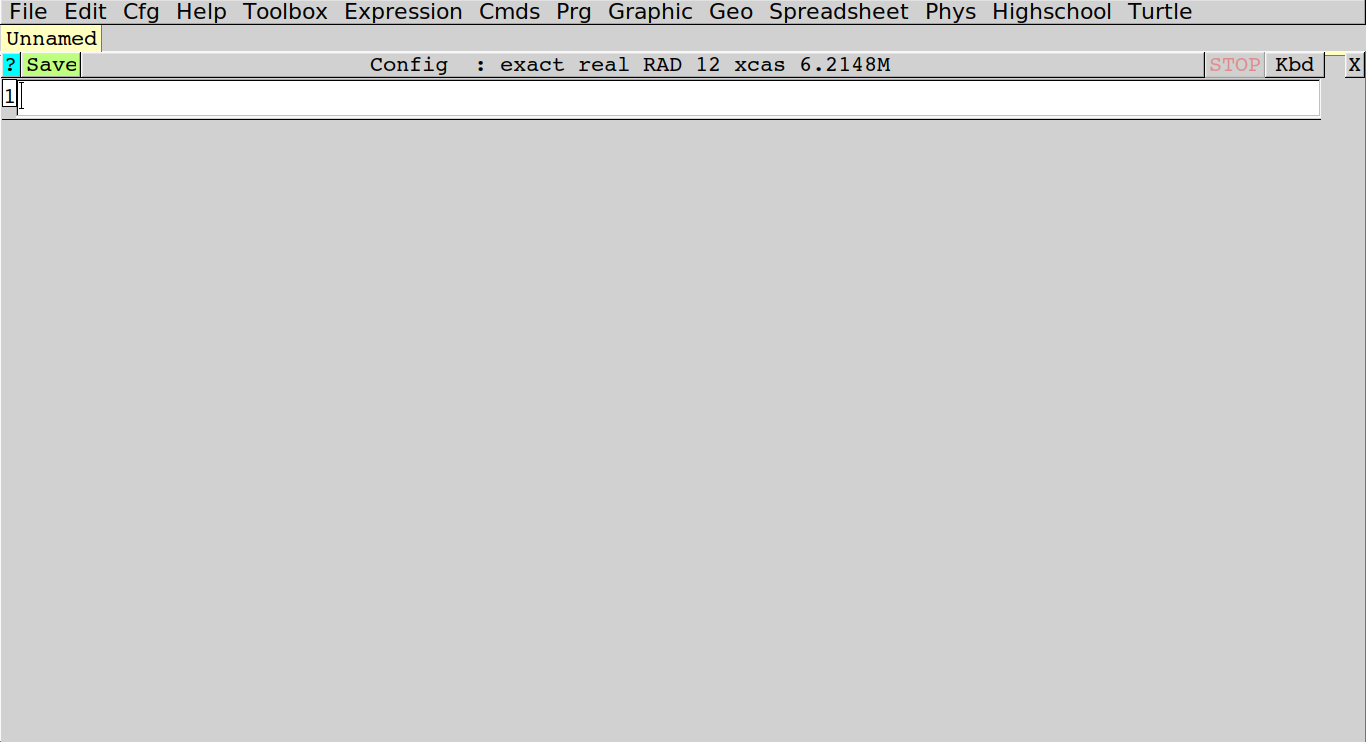
\includegraphics[width=0.75\textwidth]{xcas-open.png}
\end{center}
The first row will consist of the main menus; you can
save and load \texttt{Xcas} sessions, configure \texttt{Xcas} and its
interface and run various commands with entries from these menus.

The second row will contains tabs; one tab for each session that you
are running in \texttt{Xcas}.  Each tab will have the name of its
session, or \texttt{Unnamed} if the session has no name.  The first
time you start \texttt{Xcas}, there will be only one session, which
will be unnamed.

The third row will contain various buttons.
\begin{itemize}
  \item The first button, \framebox{\texttt{?}}, opens the help index
  (The same as the \texttt{Help$\blacktriangleright$Index} menu entry; see
  \secref{sssec:helpind}).
  If there is a command on the command line, the help index
  will open at this command.

  \item The second button, \framebox{\texttt{Save}}, saves the session
  in a file.  The first time you click on it you will be prompted for
  a file name ending in \texttt{.xws} in which to save the session.  The
  button will be pink if the session is not saved or if it has changed
  since the last change, it will be green once the session is saved.
  The name in the title will be the name of the file used to save the
  session.

\item The third button, which in the picture above is
  \begin{center}
  \framebox{\texttt{Config: exact real RAD 12 xcas 6.2148M}},
  \end{center}
  is a status
  line indicating the current \texttt{Xcas} configuration
  (see \secref{sec:config}).
  If the session is unsaved, it will begin with \texttt{Config:}; if the
  session is saved in a file \textit{filename.xws}, this button will
  begin with \texttt{Config }\textit{filename.xws}\texttt{:}.
  Other information on this status line:
  \begin{enumerate}
    \item \texttt{exact} or \texttt{approx}\\
    This tells you whether
    \texttt{Xcas} will give you exact values, such as
    $\sqrt{2}$, when possible or gives you decimal approximations,
    such as $1.4142135$.
    (See \secref{ssec:approx}.)

    \item \texttt{real}, \texttt{cplx} or \texttt{CPLX}.\\
    When this shows \texttt{real} (for example), then \texttt{Xcas} will by
    default only find real solutions of equations.  When this shows
    \texttt{cplx}, then \texttt{Xcas} will find complex solutions of
    equations.  When this shows \texttt{CPLX}, then \texttt{Xcas} will
    regard variables as complex; for example, it won't simplify
    \texttt{re(z)} (the real part of the variable $z$) to \texttt{z}.
    (See sections \ref{ssec:complex} and \ref{ssec:cvars}.)

    \item \texttt{RAD} or \texttt{DEG}.\\
    This tells you whether
    angles, as in trigonometric arguments, are measured in radians
    or degrees.
    (See \secref{ssec:angles}.)

    \item An integer.\\
    This tells you how many significant digits will be used in
    floating point calculations.
    (See \secref{ssec:sigdig}.)

    \item \texttt{xcas}, \texttt{python \^{}=**}, \texttt{python \^{}=xor},
    \texttt{maple}, \texttt{mupad}, or \texttt{ti89}.\\
    This tells you what syntax
    \texttt{Xcas} will use.  \texttt{Xcas} can be set to emulate the
    languages of Python, Maple, MuPAD, or the TI89 series of calculators.
    (See \secref{ssec:lang}.)

    \item The last item tells you how much memory \texttt{Xcas} is using.
  \end{enumerate}
  Clicking on this status line button opens a window where
  you can configure the settings shown on this line as well as some
  other settings; you can also open the window with the menu item
  \texttt{Cfg$\blacktriangleright$CAS Configuration}
  (see \secref{ssec:confcomp}).

  \item The fourth button, \framebox{\texttt{STOP}} (in red), is used
  to halt a computation which is running on too long.

  \item \label{enum:kbd}
  The fifth button, \framebox{\texttt{Kbd}}, toggles an
  on-screen scientific keyboard at the bottom of the window.
  \begin{center}
    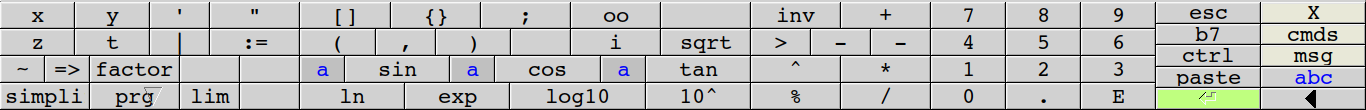
\includegraphics[width=0.75\textwidth]{xcas-scientific-keyboard.png}
  \end{center}
  Along the right hand side of the keyboard are some keys that can
  be used to change the keyboard.
  \begin{itemize}
    \item The \texttt{X} key hides the
    keyboard, just like pressing the \framebox{\texttt{Kbd}} button again.

    \item The \texttt{cmds} key toggles a menu bar at the bottom of the
    screen which can be used as an alternate menu or persistent
    submenu.  This bar will contain buttons \texttt{home},
    \texttt{<{}<}, some menu titles, \texttt{>{}>}, \texttt{var},
    \texttt{cust} and \texttt{X}.

    The \texttt{<{}<} and \texttt{>{}>} buttons scroll through menu
    items.  Clicking on one of the menu buttons will perform the
    appropriate action or replace the menu items by its submenu items.
    When submenu items appear, there will also be a \texttt{BACK}
    button to return to the previous menu.  Clicking on the
    \texttt{home} button returns the menu buttons to the main menu.

    After the menu buttons is a \texttt{var} button.  This replaces
    the menu buttons by buttons representing the variables that you
    have defined.  After that is a \texttt{cust} button, which
    displays commands that you store in a list variable \texttt{CST}
    (see section \ref{ssec:CST}).

    The last button, \texttt{X}, closes the menu bar.

    \item
    The \texttt{msg} key brings up a message window at the bottom
    of the window which will give you helpful messages; for example, if
    you save a graphic, it will tell you the name of the file it is
    saved in and how to include it in a \LaTeX{} file.

    \item The \texttt{abc} key toggles the keyboard between the
    scientific keyboard and an alphabetic keyboard.
  \end{itemize}

  \item The fifth button, \framebox{\texttt{X}}, closes the current
  session.
\end{itemize}

\section{Getting help}

\texttt{Xcas} is an extensive program, but using it is simplified with
several different ways of getting help.  The help menu (see section
\ref{ssec:helpmenu}) has several submenus for various forms of help,
some of which are mentioned below.

\subsubsection{Tooltips\label{ssec:ttips}}

If you hover the mouse cursor over certain parts of the \texttt{Xcas}
window, a temporary window will appear with information about the
part.  For example, if you move the mouse cursor over the status line,
you will get a message saying \texttt{Current CAS status.  Click to
modify}.

If you type a function name in the \texttt{Xcas} command line, a
similar temporary window will appear with information about the
function.

\subsubsection{HTML help\label{sssec:htmlhelp}}

If you press the \texttt{F12} key, you will get a window which you can
use to search the html version of the manual.  You can also open this
window with the menu entry \texttt{Help$\blacktriangleright$Find word
in HTML help}.

The HTML help window has a search area; if you type a string in that
area you will be given a list of help topics that contain that string.
If you choose a topic and click \texttt{View}, your web browser will
show the appropriate page of the manual.


\subsubsection{The help index\label{sssec:helpind}}

If you click on the \framebox{\texttt{?}} button on the status line
you will get the help index.  You can also get the help index with the
menu item \texttt{Help$\blacktriangleright$Index}.

The help index is a list of the \texttt{giac} function and variable
names.
\begin{center}
  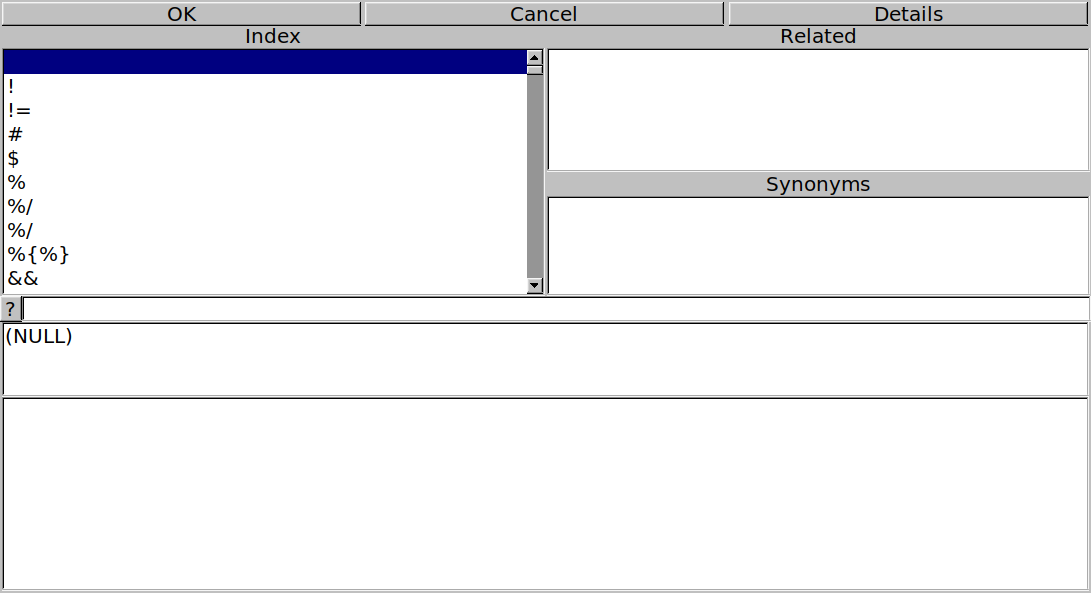
\includegraphics[width=0.75\textwidth]{xcas-help-index.png}
\end{center}
You can scroll through the help index items and click on the word that
you want.  There is also a line in the help index window that you can
use to search the index; you can enter some text and be taken to the
part of the index with the words that begin with that text.  The \texttt{?}
button next to this search line will open the HTML help window.

If you select a function or variable name, a list of related words
(names of functions or variables) and a list of synonymous words will
appear in regions to the right.
\begin{center}
  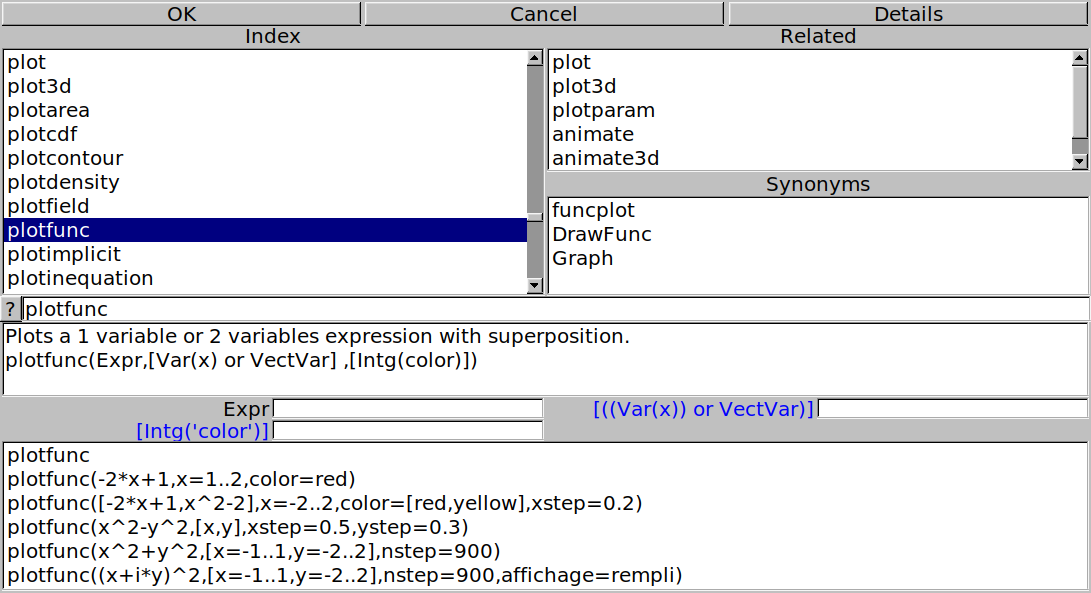
\includegraphics[width=0.75\textwidth]{xcas-help-index-plotfunc.png}
\end{center}
Below the search line, there will be an area which will have a brief description
of the chosen term as well as how to call it.  If the term is a
command name, the calling sequence will be given as the command name
with the arguments within parentheses separated by commas.  Any
optional arguments will be shown within brackets.  In the above
example, the first argument to \texttt{plotfunc} is an expression,
representing the function to be graphed.  There is an optional second
argument, which is either a variable name (which defaults to
\texttt{x}) or a vector of variable names for multivariable functions.
Finally, there is an optional third argument which can be used to
specify a color for the graph.

Below the brief description will be some entry fields that you can use
to enter the arguments.  If you fill them out and press the enter key,
the command with the arguments filled out will be put on the command
line.

Below the entry fields for the arguments will be a list of examples of
the command being used.  If you click on one of these examples, it
will be put on the command line.

A more thorough description of the function and its arguments is
available with the \texttt{Details} button at the top of the help
index, which will open the relevant part of the manual in your
browser.  Alternatively, if you click on the \framebox{\texttt{?}}
button next to the search line, you will be taken to the HTML help
window.

You can also open the help index in the following ways:
\begin{itemize}
  \item
  You can press the tab key while at the \texttt{Xcas}
  command line.\\
  If you have entered part of a command name, you will be at the part
  of the index with words that begin with the text that you entered.

  \item
  You can select a command from one of the menus.  If \texttt{Auto
  index help} is chosen (see \secref{sec:mconf}), then the help index
  will open with the command chosen.
\end{itemize}

\subsubsection{\texttt{findhelp}
\index{findhelp}}

You can get help from \texttt{Xcas} by using the \texttt{findhelp}
function.  If you enter \texttt{findhelp(}\textit{function}\texttt{)}
(or equivalently \texttt{?}\textit{function}) at the command input,
where \textit{function} is the name of a \texttt{giac} function, then
some notes on \textit{function} will appear in the answer portion and
the appropriate page of the manual will appear in your web browser.

\section{The menus}

The menus provide different ways to work with \texttt{Xcas} and its
sessions, as well as ways of inserting functions and constants into
the current session.  Selecting a menu item corresponding to a
function or constant brings up the help index (see section
\ref{sssec:helpind}) with the chosen function or constant selected.

\subsection{The \texttt{File} menu}

The \texttt{File} menu contains commands that are used to save
sessions, save parts of sessions, and load previously saved sessions.
This menu contains the following entries:
\begin{itemize}
  \item
  \texttt{New Session}\\
  This creates and opens a new session.\\
  The new session will be in a new tab, which will be labeled
  \texttt{Unnamed} until you save it (using the menu item
  \texttt{File$\blacktriangleright$Save} or the keystroke
  \texttt{Alt+S}).

  \item
  \texttt{Open}\\
  This allows you to open a previously saved session.\\
  There will be a submenu with a list of saved session files in the
  primary directory (see \secref{ssec:wdir}) that you can open,
  as well as a \texttt{File} item which will open a directory browser
  you can use to find a session file.  This directory browser can also
  be opened with \texttt{Alt-O}.

  \item
  \texttt{Import}\\
  This allows you to open a session that
  was created with the Maple CAS, a TI89 calculator or a Voyage200
  calculator.  You can execute this session with the
  \texttt{Edit$\blacktriangleright$Execute Session} menu entry, but it
  may be better to execute the commands one at a time to see if any
  modifications need to be done.

  \item
  \texttt{Clone}\\
  This creates a copy of the current session in a Firefox
  interface; either using the server at
  \url{http://www-fourier.ujf-grenoble.fr/~parisse/xcasen.html}
  (\texttt{Online}) or a local copy (\texttt{Offline}).

  \item
  \texttt{Insert}\\
  This allows you to insert a previously saved session, a link to a
  Firefox session, or a previously saved figure, spreadsheet or program.

  \item
  \texttt{Save} (\texttt{Alt+S})\\
  This saves the current session.

  \item
  \texttt{Save as}\\
  This saves the current session under a name that you choose.

  \item
  \texttt{Save all}\\
  This saves all of the sessions.

  \item
  \texttt{Export as}\\
  This allows you to save the current session in different
  formats; either in \texttt{KhiCas} (which is \texttt{giac} ported to run
  on various calculators) format, standard \texttt{Xcas} format, \texttt{Xcas}
  with Python syntax format, Maple format, MuPAD format or TI89 format.

  \item
  \texttt{Kill}\\
  This kills the current session.

  \item
  \texttt{Print}\\
  This allows you to create an image of the session in various ways.\\
  The \texttt{Preview} menu item saves an image of the current session in a file
  that you name.  The \texttt{To printer} item sends an image of the current
  session to the printer.  The \texttt{Preview selected levels} item
  saves the images of the commands and outputs of the selected levels,
  each in a separate file.

  \item
  \texttt{LaTeX}\\
  This has submenu items that render the session in \LaTeX{} and give you the
  result in various ways.  The \texttt{LaTeX preview} menu item displays a
  compiled \LaTeX{} version of the current session.  The \texttt{LaTeX
  print} item saves a copy of the session in \LaTeX{} form, along with
  the compiled version in various formats.  The \texttt{LaTeX print
  selection} does the same as \texttt{LaTeX print}, but only for the
  selected levels.

  \item
  \texttt{Screen capture}\\
  This creates a screenshot that is saved in various formats.

  \item \texttt{Quit and update Xcas}\\
  This quits \texttt{Xcas} after checking for a newer version.

  \item \texttt{Quit} (\texttt{Ctrl+Q})\\
  This quits \texttt{Xcas}.
\end{itemize}

\subsection{The \texttt{Edit} menu}

The \texttt{Edit} menu contains commands that are used to execute and
undo parts of the current session.  This menu contains the following
entries:
\begin{itemize}
  \item \texttt{Execute worksheet} (\texttt{Ctrl-F9})\\
  This recalculates each level in the session.

  \item \texttt{Execute worksheet with pauses}\\
  This recalculates each level in the session, pausing between
  calculations.

  \item \texttt{Execute below}\\
  This recalculates the current level and each level below it.

  \item \texttt{Remove answers below}\\
  This removes the answers to the current level and the levels
  below it.

  \item \texttt{Undo} (\texttt{Ctrl+Z})\\
  This undoes the latest edit done to the levels, including a
  deletion of a level.  It can be repeated to undo more than one edit.

  \item \texttt{Redo} (\texttt{Ctrl+Y})\\
  This redoes the undone editing.

  \item \texttt{Paste}\\
  This pastes the contents of the system clipboard to the cursor
  position.

  \item \texttt{Del selected levels}\\
  This deletes any entry levels that you have selected.

  \item \texttt{selection -> LaTeX} (\texttt{Ctrl+T})\\
  This puts a \LaTeX{} version of the
  selection (level, part of a level, or answer selected by clicking
  and dragging the mouse) on the system clipboard.

  \item \texttt{New entry} (\texttt{Alt+N})\\
  This inserts a new entry level above the current one.

  \item \texttt{New parameter} (\texttt{Ctrl+P})\\
  This brings up a window in which you can enter a name and
  conditions for a new parameter.

  \item \texttt{Insert newline}\\
  This inserts a newline below the cursor.  Note that simply
  typing return will evaluate the current entry rather
  than inserting a newline.

  \item \texttt{Merge selected levels}\\
  This merges the selected levels into a single level.
\end{itemize}

\subsection{The \texttt{Cfg} menu}

The \texttt{Cfg} menu contains commands that are used to set the
behaviour of \texttt{Xcas}.  This menu contains the following entries:
\begin{itemize}
  \item \texttt{Cas configuration}\\
  This opens a window that allows you to configure how
  \texttt{Xcas} performs calculations (see
  \secref{ssec:confcomp}).  This is the same window you
  get when you click on the status line.

  \item \texttt{Graph configuration}\\
  This opens a window that allows you to configure the default
  settings for a graph (see \secref{ssec:confgraph}).
  This includes such things as the initial
  ranges of the variables.  Each graph also has a \texttt{cfg}
  button to configure the settings on a per graph basis.

  \item \texttt{General configuration}\\
  This opens a window that allows you to configure various
  non-computational aspects of \texttt{Xcas}, such as the fonts, the
  default paper size, and the like (see \secref{sec:mconf}).

  \item \texttt{Mode (syntax)}\\
  This changes the default syntax (see \secref{ssec:lang}).
  By default, \texttt{Xcas} uses its own syntax, but you can change it
  to Python syntax, Maple syntax, MuPAD syntax or TI89 syntax.

  \item \texttt{Show}\\
  This displays parts of \texttt{Xcas}.
  \begin{itemize}
    \item   \texttt{DispG}\\
    This shows the graphics display screen; which has
    all graphical commands from the session together on one screen.

    \item \texttt{keyboard}\\
    This shows the on-screen keyboard; the same as clicking on the
    \texttt{Kbd} button on the status line (see \secref{sec:swin},
    item \ref{enum:kbd}).

    \item \texttt{bandeau}\\
    This shows the menu buttons at the bottom of the window;
    the same as clicking on \texttt{cmds} on the on-screen keyboard
    (see \secref{sec:swin}, item \ref{enum:kbd}).

    \item \texttt{msg}\\
    This shows the messages window; the same as clicking on
    \texttt{msg} on the on-screen keyboard (see \secref{sec:swin},
    item \ref{enum:kbd}).
  \end{itemize}

  \item \texttt{Hide}\\
  This hides the same items that you can show with \texttt{Show}.

  \item \texttt{Index language}\\
  This allows you to choose a language in which to display the help index.

  \item \texttt{Colors}\\
  This allows you to choose colors for various parts of the display.

  \item \texttt{Session font}\\
  This allows you to choose a font for the sessions.

  \item \texttt{All fonts}\\
  This allows you to choose fonts for the session, the main menu and
  the keyboard.

  \item \texttt{browser}\\
  This allows you to choose a browser that \texttt{Xcas} will use when
  needed.  If this is blank, then \texttt{Xcas} will use its own
  internal browser.

  \item \texttt{Save configuration}\\
  This saves the configurations that you chose with the
  \texttt{Cfg} menu or chose by clicking on the status line.
\end{itemize}

\subsection{The \texttt{Help} menu\label{ssec:helpmenu}}

The \texttt{Help} menu contains commands that let you get information
about \texttt{Xcas} from various sources. This menu contains the
following entries:
\begin{itemize}
  \item \texttt{Index}\\
  This brings up the help index (see \secref{sssec:helpind}).

  \item \texttt{Find word in HTML help} (\texttt{F12})\\
  This brings up a page which helps you search for keywords in
  the html documentation that came with \texttt{Xcas} (see
  \secref{sssec:htmlhelp}).  The help will be displayed in your browser.

  \item \texttt{Interface}\\
  This brings up a tutorial for the \texttt{Xcas} interface.  The
  tutorial will be displayed in your browser.

  \item \texttt{Reference card, fiches}\\
  This brings up a pdf reference card for
  \texttt{Xcas}.  The card will be displayed in your browser.

  \item \texttt{Manuals}\\
  This allows you to choose from a variety of manuals for \textsc{Xcas},
  which will appear in your browser.
  \begin{itemize}
  \item \texttt{CAS reference}\\
  This brings up the manual for \texttt{Xcas}.

  \item \texttt{Algorithmes (HTML)}\\
  This brings up a manual for the algorithms used by \texttt{Xcas}.

  \item \texttt{Algorithmes (PDF)}\\
  This brings up a pdf version of the manual for the algorithms
  used by \texttt{Xcas}.

  \item \texttt{Geometry}\\
  This brings up a manual for two-dimensional geometry in
  \texttt{Xcas}.

  \item \texttt{Programmation}\\
  This brings up a manual for programming in \texttt{Xcas}.

  \item \texttt{Simulation}\\
  This brings up a manual for statistics and using the
  \texttt{Xcas} spreadsheet.

  \item \texttt{Turtle}\\
  This brings up a manual for using the \texttt{Turtle} drawing
  screen in \texttt{Xcas}.

  \item \texttt{Exercices}\\
  This brings up a page of exercises that you can do with
  \texttt{Xcas}.

  \item \texttt{Amusement}\\
  This brings up a page of mathematical amusements that you can
  work through with \texttt{Xcas}.

  \item \texttt{PARI-GP}\\
  This brings up documentation for the GP/PARI functions.
  \end{itemize}

  \item \texttt{Internet}\\
  The \texttt{Internet} menu contains menu items that take you to
  various web pages related to \texttt{Xcas}.  Among them are the
  following entries:
  \begin{itemize}
    \item \texttt{Forum}\\
    This takes you to the \texttt{Xcas} forum.

    \item \texttt{Update help}\\
    This installs updated help files (retrieved from the
    \texttt{Xcas} website).
  \end{itemize}
   There are also several menu items that take you to \texttt{Xcas} related pages written
   in French; namely:
  \begin{itemize}
    \item \texttt{Aide-memoire lycee}\\
     This takes you to a paper discussing \texttt{Xcas} and high
     school.

    \item \texttt{Documents pedagogiques lycee}\\
     This takes you to a page on the \texttt{Xcas} website with a
     list of useful links.

    \item \texttt{Documents algorithmique}\\
    This takes you to a page on the \texttt{Xcas} website with a
    list of links.

    \item \texttt{Site Lycee de G. Connan}\\
    This takes you to a page about a free book written by
    Guillaume Connan teaching algorithms to high school students.

    \item \texttt{Site Lycee de L. Briel}\\
    This takes you to a website about \texttt{Xcas} for high
    school students.

    \item \texttt{Calcul formel au lycee, par D. Chevallair}\\
    This takes you to a pdf file discussing the use of
    \texttt{Xcas} in high school.

    \item \texttt{Site de F. Han}\\
    This takes you to a website by Frederic Han about
    \texttt{Xcas} and a QT frontent for \texttt{giac}.

    \item \texttt{Ressources Capes}\\
    This takes you to a website with various external sources.

    \item \texttt{Ressources Agregation externe}\\
    This takes you to a collection of external resources.

    \item \texttt{Ressources Agregation interne}\\
    This takes you to a page on the \texttt{Xcas} website.
   \end{itemize}

\item \texttt{Start with CAS}\\
  This menu has the following entries:
  \begin{itemize}
    \item \texttt{Tutorial}\\
    This opens up the tutorial.
    \item \texttt{Solutions}\\
    This opens up the solutions to the exercises in the tutorial.
  \end{itemize}

  \item \texttt{Tutoriel algo}\\
  This opens up a tutorial on algorithms and programming with
  \texttt{Xcas}.

  \item \texttt{Rebuild help cache}\\
  This rebuilds the help index.

  \item \texttt{About}\\
  This displays a message window with information about \texttt{Xcas}.

  \item \texttt{Examples}\\
  This allows you to choose from a variety of example worksheets,
  which will then be copied to your current directory and opened.
\end{itemize}

\subsection{The \texttt{Toolbox} menu}

The \texttt{Toolbox} menu contains commands that are used to insert
operators into the session.  This menu includes the following entries:

\begin{itemize}
  \item \texttt{New entry} (\texttt{Alt+N})\\
  This inserts a new level.

  \item \texttt{New comment} (\texttt{Alt+C})\\
  This inserts a new comment level.
\end{itemize}
The other entries let you insert mathematical operations into
the current level. If \texttt{Auto index help} is chosen
(see \secref{sec:mconf}), then the help index will open
help index (see \secref{sssec:helpind})
with the chosen command selected.

\subsection{The \texttt{Expression} menu}

The \texttt{Expression} menu contains commands that are used to
transform expressions.  The first entry is \texttt{New expression}
(which is equivalent to \texttt{Alt+E}), which inserts a new level and
brings up the on-screen keyboard (see \secref{sec:swin}, item
\ref{enum:kbd}).  The rest of the entries can be used to insert
various transformations.

\subsection{The \texttt{Cmds} menu}

The \texttt{Cmds} menu contains various \texttt{giac} functions and
constants separated into categories.  If \texttt{Auto index help} is
chosen (see \secref{sec:mconf}), then when you select a function or
constant, the help index (see \secref{sssec:helpind}) opens with the
function or constant selected, which can be used to insert the entry
on the command line.  Otherwise, the constant or function will be
inserted on the command line.

\subsection{The \texttt{Prg} menu}

The \texttt{Prg} menu contains commands that are used to write
\texttt{giac} programs.  The first entry,
\texttt{Prg$\blacktriangleright$New program} (equivalent to
\texttt{Alt+P}), inserts a program level and brings up the program
editor (see \secref{ssec:proged}).The other entries are useful
commands for writing \texttt{giac} programs.

\subsection{The \texttt{Graphic} menu}

The \texttt{Graphic} menu contains commands that are used to create
graphs.  The first entry,
\texttt{Graphic$\blacktriangleright$Attributs} (equivalent to
\texttt{Alt+K}), brings up a window containing different attributes of
the graph (such as line width, color, etc.).  The other entries are
commands for creating and manipulating graphs.

\subsection{The \texttt{Geo} menu}

The \texttt{Geo} menu contains commands that are used to work with
two- and three-dimensional geometric figures.  The first two entries,
\texttt{Geo$\blacktriangleright$New figure 2d} (equivalent to
\texttt{Alt+G}) and \texttt{Geo$\blacktriangleright$New figure 3d}
(equivalent to \texttt{Alt+H}) create levels for two- and
three-dimensional figures, respectively. (See
\secref{sec:graphscreen}.) The other menu items are for working with
the figures.

\subsection{The \texttt{Spreadsheet} menu}

The \texttt{Spreadsheet} menu contains commands that are used to work
with spreadsheets.  (See See \secref{sec:spreadsheet}.) The first menu
item, \texttt{Spreadsheet$\blacktriangleright$New spreadsheet}
(equivalent to \texttt{Alt+T}), brings up a window where you can set
the size and other attributes of a spreadsheet, after which one will
be created.  The submenus contain commands for working with
spreadsheets.  Notice that the spreadsheet itself will have menus that
are the same as these submenus.

\subsection{The \texttt{Phys} menu}

The \texttt{Phys} menu contains submenus with various categories of
constants, as well as functions for converting units.

\subsection{The \texttt{Highschool} menu}

The \texttt{Highschool} menu contains computer algebra commands that
are useful at different levels of highschool.  There is also a
\texttt{Program} submenu with some program control functions.

\subsection{The \texttt{Turtle} menu}

The \texttt{Turtle} menu contains the commands that are used to create
and control a Turtle screen.  The first menu item,
\texttt{Turtle$\blacktriangleright$New turtle}, creates a Turtle
drawing screen.  The other menu items contain commands for working
with the screen.

\section{Configuring \texttt{Xcas}\label{sec:config}}

\subsection{The number of significant digits: \texttt{Digits} \texttt{DIGITS}
\index{Digits}
\index{DIGITS}
\label{ssec:sigdig}}

By default, \texttt{Xcas} uses and displays \texttt{12} significant
digits, but you can set the number of digits to other positive
integers.  If you set the number of significant digits to a number
less than \texttt{14}, then \texttt{Xcas} will use the computer's
floating point hardware, and so calculations will be done to more
significant digits than you asked for, but only the number of digits
that you asked for will be displayed.  If you set the number of
significant digits to \texttt{14} or higher, then both the
computations and the display will use that number of digits.

You can set the number of significant digits for \texttt{Xcas} by
using the CAS configuration screen (see \secref{ssec:confcomp}).  The
number of significant digits is stored in the variable \texttt{DIGITS}
or \texttt{Digits}, so you can also set it by giving the variable
\texttt{DIGITS} a new value, as in \texttt{DIGITS:= 20}.  The value
will be stored in the configuration file (see \secref{ssec:conffile}),
and so can also be set there.

\subsection{The language mode: \texttt{xcas\_mode}
\index{xcas\_mode}
\label{ssec:lang}}

\texttt{Xcas} has its own language which it uses by default, but you
can have it use Python (with the option having the \texttt{\^{}}
character represent either exponentiation or the \textsl{exclusive or}
operator), the language used by \texttt{Maple}, \texttt{MuPAD} or the
\texttt{TI89} calculator.

You can set which language \texttt{Xcas} uses in the CAS configuration
screen (see \secref{ssec:confcomp}).  You can also set the language
with the \texttt{xcas\_mode} command.
\begin{itemize}
\item The \texttt{xcas\_mode} command takes one argument: an
integer: 0, 1, 2, 3, 256 or 512.
\begin{itemize}
  \item \texttt{xcas\_mode(0)}\\
  to use the \texttt{Xcas} language.
  \item  \texttt{xcas\_mode(1)}\\
  to use the \texttt{Maple} language.
  \item \texttt{xcas\_mode(2)}\\
  to use the \texttt{MuPAD} language.
  \item \texttt{xcas\_mode(3)}\\
  to use the \texttt{TI89} language.
  \item \texttt{xcas\_mode(256)}\\
  to use the Python language with \texttt{\^{}} representing exponentiation.
  \item \texttt{xcas\_mode(512)}\\
  to use the Python language with \texttt{\^{}} representing
  \textsl{exclusive or}.
\end{itemize}
\end{itemize}
The language you choose will be stored in the configuration file (see
\secref{ssec:conffile}), and so can also be set there.

\subsection{The units for angles: \texttt{angle\_radian}
\index{angle\_radian}
\label{ssec:angles}}

By default, \texttt{Xcas} assumes that any angles you use (for
example, as the argument to a trigonometric function) are being
measured in radians.  If you want, you can have \texttt{Xcas} use
degrees.

You can set which angle measure \texttt{Xcas} uses in the CAS
configuration screen (see \secref{ssec:confcomp}). Your choice will be
stored in the variable \texttt{angle\_radian}; this will be \texttt{1}
if you measure your angles in radians and \texttt{0} if you measure
your angles in degrees.  You can also change which angle measure you
use by setting the variable \texttt{angle\_radian} to the appropriate
value.  The angle measure you want to use will be stored in the
configuration file (see \secref{ssec:conffile}), and so can also be
set there.

\subsection{Exact or approximate values: \texttt{approx\_mode}
\index{approx\_mode}
\label{ssec:approx}}

Some numbers, such as $\pi$ and $\sqrt{2}$, can't be written down
exactly as decimal numbers.  When computing with such numbers, by
default \texttt{Xcas} leaves them in exact, symbolic form.  If you
want, you can have \texttt{Xcas} automatically give you decimal
approximations for these numbers.

You can set whether or not \texttt{Xcas} gives you exact or
approximate values by using the CAS configuration screen (see
\secref{ssec:confcomp}).  Your choice will be stored in the variable
\texttt{approx\_mode}, where a value of 0 means that \texttt{Xcas}
will give you exact answers when possible and a value of 1 means that
\texttt{Xcas} will give you decimal approximations.  Your choice will
be stored in the configuration file (see section \ref{ssec:conffile}),
and so can also be set there.

\subsection{Complex numbers: \texttt{cfactor} \texttt{complex\_mode}
\index{cfactor}
\index{complex\_mode}
\label{ssec:complex}}

When factoring polynomials (see \secref{ssec:factore}), by default
\texttt{Xcas} won't introduce complex numbers if they aren't already
being used.  For example, 
\begin{center}
  \texttt{factor(x\^{}2 + 2)}
\end{center}
simply returns
\[
x^{2}+2
\]
%Output:
% \begin{center}
%   \texttt{x\^{}2 + 2}
% \end{center}
but if an expression already involves complex numbers then
\texttt{Xcas} uses them;
\begin{center}
  \texttt{factor(i*x\^{}2 + 2*i)}
\end{center}
will return
\[
\left(x-\mathrm{i} \sqrt{2}\right) \left(\mathrm{i} x-\sqrt{2}\right)
\]
%Output:
% \begin{center}
%   \texttt{(x - i*sqrt(2))*(i*x - sqrt(2))}
% \end{center}
\texttt{Xcas} can also find complex roots when complex
numbers are not present; for example, the command \texttt{cfactor}
(see \secref{ssec:factore}) will factor over the complex numbers.\\
\texttt{cFactor} is a synonym for \texttt{cfactor}.
\begin{center}
  \texttt{cfactor(x\^{}2 + 2)}
\end{center}
returns
%Output:
\[
\left(x+\mathrm{i} \sqrt{2}\right) \left(x-\mathrm{i} \sqrt{2}\right)
\]
% \begin{center}
%   \texttt{(x - i*sqrt(2))*(x + i*sqrt(2))}
% \end{center}

If you want \texttt{Xcas} to use complex numbers by default, you can
turn on complex mode.  In complex mode,
\begin{center}
  \texttt{factor(x\^{}2 + 2)}
\end{center}
returns
\[
\left(x+\mathrm{i} \sqrt{2}\right) \left(x-\mathrm{i} \sqrt{2}\right)
\]
%Output:
% \begin{center}
%   \texttt{(x - i*sqrt(2))*(x + i*sqrt(2))}
% \end{center}

You can turn on complex mode from the CAS configuration screen (see
\secref{ssec:confcomp}).  This mode is determined by the value of the
variable \texttt{complex\_mode}; if this is \texttt{1} then complex
mode is on, if this is \texttt{0} then complex mode is off. This
option will be stored in the configuration file (see
\secref{ssec:conffile}), and so can also be set there.

\subsection{Complex variables: \texttt{complex\_variables}
\index{complex\_variables}
\label{ssec:cvars}}

By default, new variables are assumed to be real; functions which work
with the real and imaginary parts of variables will assume that a
variable is real.  For example, \texttt{re} returns the real part of
its argument and \texttt{im} returns the imaginary part (see
\secref{ssec:reim}), and so
\begin{center}
  \texttt{re(z)}
\end{center}
returns
%Output:
\[
z
\]
% \begin{center}
%   \texttt{z}
% \end{center}
and
\begin{center}
  \texttt{im(z)}
\end{center}
returns
\[
0
\]
%Output:
% \begin{center}
%   \texttt{0}
% \end{center}

If you want variables to be complex by default, you can have
\texttt{Xcas} use complex variable mode.  You can set this from the
CAS configuration screen (see \secref{ssec:confcomp}).  Your choice
will be stored in the variable \texttt{complex\_variables}, where a
value of 0 means that \texttt{Xcas} will assume that variables are
real and and a value of 1 means that \texttt{Xcas} will assume that
variables are complex.  Your choice will be stored in the
configuration file (see \secref{ssec:conffile}), and so can also be
set there.

\subsection{Configuring the computations\label{ssec:confcomp}}

You can configure how \texttt{Xcas} computes by using the menu item
\texttt{Cfg$\blacktriangleright$Cas configuration} or by clicking on
the status line.  This will open a window with the following options:
\begin{enumerate}
  \item \texttt{Prog style} (default: \texttt{Xcas})\\
  This has a menu from which you can choose a different language
  to program in; you can choose from \texttt{Xcas}, \texttt{Python
  \^{}==**} (Python syntax, except that \texttt{\^{}} will be the
  exponentiation operator as in \texttt{Xcas} rather than the
  \textsl{exclusive or} operator as in Python), \texttt{Python \^{}==xor}
  (Python syntax, where \texttt{\^{}} is the \textsl{exclusive or} operator),
  \texttt{Maple}, \texttt{Mupad} and \texttt{TI89/92}.

  \item \texttt{eval} (default: 25)\\
  This has an input field where you can type in a positive integer
  specifying the maximum number of recursions allowed when evaluating
  expressions.

  \item \texttt{prog} (default: 1)\\
  This has an input field where you can type in a positive integer
  specifying the maximum number of recursions allowed when executing
  programs.

  \item \texttt{recurs} (default: 100)\\
  This has an input field where you can type in a positive integer
  specifying the maximum number of recursive calls.

  \item \texttt{debug} (default: 0)\\
  This has an input field where you can type in a 0 or 1.  If this is 1, then
  \texttt{Xcas} will display intermediate information on the
  algorithms used by \texttt{giac}.  If this is 0, then no such
  information is displayed.

  \item\label{enum:maxiter} \texttt{maxiter}  (default: 20)\\
  This has an input field where you can type in an integer specifying
  the maximum number of iterations to be used in Newton's method.

  \item\label{enum:float}  \texttt{Float format}  (default: \texttt{standard})\\
  This has a menu from which you can choose how to display
  decimal numbers.  Your choices will be:
  \begin{itemize}
  \item \texttt{standard}  In standard notation, a number will be
  written out completely without using exponentials; for example,
  \texttt{15000.12} will be displayed as \texttt{15000.12}.
  \item \texttt{scientific}  In scientific notation, a number will be
  written as a number between 1 and 10 times a power of ten; for example,
  \texttt{15000.12} will be displayed as \texttt{1.500012000000e+04}
  (where the number after \texttt{e} indicates the power of 10).
  \item \texttt{engineer}  In engineering notation, a number will be
  written as a number between 1 and 1000 times a power of ten, where
  the power of 10 is a multiple of three.  For example,
  \texttt{15000.12} will be displayed as \texttt{15.00012e3}.
  \end{itemize}

  \item\label{enum:digs} \texttt{Digits}  (default: 12)\\
  This has an input field where you can type in a positive integer which will
  indicate the number of significant digits that \texttt{Xcas} will use.

  \item\label{enum:eps} \texttt{epsilon}  (default: 1e-12)\\
  This has an input field where you can type in a floating point number
  which will be the value of epsilon used by \texttt{epsilon2zero},
  which is a function that replaces numbers with absolute value less
  than epsilon by 0 (see \secref{ssec:epsilon2zero}).

  \item \texttt{proba}  (default: 1e-15)\\
  This has an input field where you can type in a floating point number.
  If this number is greater than zero, then in some cases
  \texttt{giac} can use probabilistic algorithms and give a result
  with probability of being false less than this value.  (One such
  example of a probabilistic algorithm that \texttt{giac} can use is
  the algorithm to compute the determinant of a large matrix with
  integer coefficients.)

  \item \texttt{approx}  (default: unchecked)\\
  This has a checkbox.  If the box is checked, then exact
  numbers such as $\sqrt{2}$ will be given a floating point approximation.  If
  the box in unchecked, then exact values will be used when possible.
  (See \secref{ssec:approx}.)

  \item \texttt{autosimplify}  (default: 1)\\
  This has an input field where you can type in 0, 1 or 2.  A value of 0
  means no automatic simplification will be done, a value of 1 means
  grouped simplification will be automatic.  A value of 2 means that
  all simplification will be automatic.

  \item \texttt{threads}  (default: 1)\\
  This has an input field where you can enter a positive integer to
  indicate the number of threads (for a possible future threaded
  version).

  \item\label{enum:base} \texttt{Integer basis}  (default: 10)\\
  This has a menu from which you can choose an integer base
  to work in; your choices will be 8, 10 and 16.

  \item \texttt{radian} (default: \texttt{checked})\\
  This has a checkbox.  If the box is checked, then angles
  will be measured in radians, otherwise they will be measured in
  degrees.

  \item \texttt{Complex}  (default: \texttt{unchecked})\\
  This has a checkbox.  If this box is checked, then
  \texttt{giac} will work in complex mode, meaning, for example, that
  polynomials will be factored with complex numbers if necessary.

  \item \texttt{Cmplx\_var}  (default: \texttt{unchecked})\\
  This has a checkbox.  If this box is checked, then
  variables will by default be assumed to be complex.  For example,
  the expression \texttt{re(z)} won't be simplified, it will return
  \texttt{re(z)}.  If this box is unchecked, then variables by default
  will be assumed to be real, and so \texttt{re(z)} will be
  simplified to \texttt{z}.

  \item \texttt{increasing power}  (default: \texttt{unchecked})\\
  This has a checkbox.  If this box is checked, then
  polynomials will be written out in increasing powers of the
  variable; otherwise they will be written in decreasing powers.

  \item\label{enum:trig} \texttt{All\_trig\_sol}  (default: \texttt{unchecked})\\
  This has a checkbox.  If this box is checked, then \texttt{Xcas} will
  give the complete solutions of trigonometric equations.  For
  example, the solution of $\cos(x)=0$ will be given as
  $[(2n\_{0}\pi + \pi)/2]$, where $n_{0}$ can be any
  integer.  If this box is unchecked, then only the primary solutions
  of trigonometric equations will be given.  For example, the
  solutions of $\cos(x)=0$ will be the pair $[-\pi/2,\pi/2]$.

  \item \texttt{Sqrt}  (default: \texttt{checked})\\
  This has a checkbox.  If this box is checked, then the
  \texttt{factor} command will factor second degree polynomials, even
  when the roots are not in the field determined by the coefficients.
  For example, \texttt{factor(x\^{}2 - 3)} will return %Output:
  $\left(x-\sqrt{3}\right) \left(x+\sqrt{3}\right)$.
%  \texttt{(x - sqrt(3))*(x + sqrt(3))}.
  If this box is unchecked, then \texttt{factor(x\^{}2 - 3)}  will return $x^{2}-3$.
  %\texttt{x\^{}2 - 3}.
\end{enumerate}
This page also has buttons for applying the settings, saving the
settings for future sessions, canceling any new settings, and restoring
the default settings.

\subsection{Configuring the graphics\label{ssec:confgraph}}

You can configure each graphics screen by clicking on the \texttt{cfg}
button on the graphics screen's control panel to the right of the
graph.  You can also change the default graphical configuration using
the the menu item \texttt{Cfg$\blacktriangleright$Graph
configuration}. You will then be given a window in which you can
change the following options:
\begin{itemize}
  \item \texttt{X-} and \texttt{X+}\\
  These determine the $x$ values for which calculations will be
  done.

 \item \texttt{Y-} and \texttt{Y+}\\
 These determine the $y$ values for which calculations will be done.

 \item \texttt{Z-} and \texttt{Z+}\\
 These determine the $z$ values for which calculations will be done.

 \item \texttt{t-} and \texttt{t+}\\
 These determine the $t$ values for which calculations will be
 done; when plotting parametric curves, for example.

 \item \texttt{WX-} and \texttt{WX+}\\
 These determine the range of $x$ values for the viewing window.

 \item \texttt{WY-} and \texttt{WY+}\\
 These determine the range of $y$ values for the viewing window.

 \item \texttt{TX} and \texttt{TY}\\
  These determine the tick ranges on the $x$- and $y$-axes.

  \item \texttt{class\_min}\\
  This determines the minimum size of a statistics class.

  \item \texttt{class\_size}\\
  This determines the default size of a statistics class.

  \item \texttt{autoscale}\\
  When checked, the graphic will be autoscaled.

  \item \texttt{ortho}\\
  When checked, all axes of the graphic will be scaled equally.

  \item \texttt{>W} and \texttt{W>}\\
  These are convenient shortcuts to copy the \texttt{X-}, \texttt{X+},
  \texttt{Y-} and \texttt{Y+} values to  \texttt{WX-}, \texttt{WX+},
  \texttt{WY-} and \texttt{WY+}, or the other way around.
\end{itemize}
Note that the viewing window is not the same as the calculation
window; if the calculation window is larger than the visible window,
then you can scroll to bring other parts of the calculation window
into view.

This page also has buttons for applying the settings, saving the
settings for future sessions, or canceling any new settings.

\subsection{More configuration\label{sec:mconf}}

You can configure other aspects of \texttt{Xcas} (besides the
computational aspects and graphics) using the the menu item
\texttt{Cfg$\blacktriangleright$General configuration}. You will then
be given a window in which you can change the following options:
\begin{itemize}
  \item \texttt{Font}\\
  This lets you choose a session font, the same as choosing the menu
  item \texttt{Cfg$\blacktriangleright$Session font}.

  \item \texttt{Level}\\
  This determines what type of level should be open when you start
  a new session.

  \item \texttt{browser}\\
  This determines what browser \texttt{Xcas} will use when it
  requires one, for example when displaying help.  If this is empty,
  \texttt{Xcas} will use its built-in browser.

  \item \texttt{Auto HTML help}\\
  If this box is checked, then whenever you choose a function from a menu,
  a help page for that function will appear in your browser.
  Regardless of whether this box is checked or not, the help page will
  also appear in your browser if you enter \texttt{?}\textit{function}
  from a command box.

  \item \texttt{Auto index help}
  If this box is checked, then whenever you choose a command from a
  menu, the help index page for that function will appear.  This is
  the same page you get when you choose the command from the help
  index.  (See \secref{sssec:helpind}.)

  \item \texttt{Print format}\\
  This determines the paper size for printing and saving files.
  There is also a button you can use to have the printing done in
  landscape mode; if this button is not checked, the printing will be
  done in portrait.

  \item \texttt{Disable Tool tips}\\
  If this box is checked, \texttt{Xcas} will stop displaying tool tips
  (see \secref{ssec:ttips}).

  \item \texttt{rows} and \texttt{columns}\\
  These determine the default number of rows and columns for the
  matrix editor and spreadsheet (see \secref{sec:spreadsheet}).

  \item \texttt{PS view}\\
  This determines what program is used to preview Postscript files.

  \item \texttt{Step by step}\\
  If this is checked, then \texttt{Xcas} will not save context
  information.

  \item \texttt{Proxy}\\
  This sets a proxy server for updates.

\end{itemize}

\subsection{The configuration file: \texttt{widget\_size} \texttt{cas\_setup} \texttt{xcas\_mode} \texttt{xyztrange}
\index{widget\_size}
\index{cas\_setup}
\index{xcas\_mode}
\index{xyztrange}
\label{ssec:conffile}}

When you save changes to your configuration, they are stored in a
configuration file, which will be \texttt{.xcasrc}\index{.xcasrc} in
your home directory in Unix and \texttt{xcas.rc}\index{xcas.rc} in
Windows.  This file will have four functions -- \texttt{widget\_size},
\texttt{cas\_setup}, \texttt{xcas\_mode} and \texttt{xyztrange} --
which determine the configuration and which are evaluated when
\texttt{Xcas} starts.

The \texttt{widget\_size} command sets properties of the opening
\texttt{Xcas} window.
\begin{itemize}
\item
\texttt{widget\_size} takes between 1 and 12 arguments. The arguments
(in order) are:
\begin{itemize}
  \item \textit{Font size.}  The first argument is a positive integer
  specifying the font size.  Optionally, this can be a bracketed list
  whose first number indicates the font and the second the font size.
  \item \textit{Horizontal and vertical offset.}  The second and third
  arguments are horizontal and vertical distances in pixels from the
  upper left hand corner of the screen.   They specify where the upper
  left corner of the \texttt{Xcas} window is when it opens.
  \item \textit{Window size.}  The fourth and fifth arguments specify the width and height in
  pixels of the \texttt{Xcas} window when it opens.
  \item  \textit{Keyboard} (see \secref{sec:swin}, item
  \ref{enum:kbd}).  The sixth argument is either 0 or 1; a 1 indicates
  that the on-screen keyboard will be open when \texttt{Xcas} starts,
  a 0 indicates that the keyboard will be hidden.
  \item \textit{Open browser.} The seventh argument is either 0 or 1;
  a 1 indicates that the browser will be automatically opened to
  display help for the selected command in the menu or index, a 0
  indicates that the browser will not be automatically opened.
  \item \textit{Message window} (see \secref{sec:swin}, item \ref{enum:kbd}).
  The eighth argument is either 0 or 1;
  a 1 indicates that \texttt{Xcas} will open with the message window,
  a 0 indicates that \texttt{Xcas} will open without the message
  window.
  \item The ninth argument is currently not used.
  \item \textit{Browser name.} The tenth argument is a string with the
  name of the browser to use to read the help pages.  A value of
  \texttt{"builtin"} means that \texttt{Xcas} will use a small browser
  built into \texttt{Xcas}.
  \item \textit{Starting level} (see \secref{sec:levels}).  The eleventh
  argument indicates what level \texttt{Xcas} will start at; a 0
  means command line, a 1 means program editor, a
  2 means spreadsheet, and a 3 means a 2-d geometry screen.
  \item \textit{Postscript previewer.} The twelfth argument is a
  string with the name of a program for postscript previews; for
  example, \texttt{"gv"}.
\end{itemize}
\end{itemize}

The \texttt{cas\_setup} command determines how computations will be
performed.
\begin{itemize}
\item
\texttt{cas\_setup} takes nine arguments. The arguments (in
order) are:
\begin{itemize}
  \item \textit{Approximate mode} (see \secref{ssec:approx}).  A 1
  means \textit{Xcas} works in approximate mode, a 0 means exact mode.
  \item \textit{Complex variables} (see \secref{ssec:complex}).  A 1
  means \textit{Xcas} works with complex variables, a 0 means real
  variables.
  \item \textit{Complex mode} (see \secref{ssec:complex}).
  A 1 means \texttt{Xcas} works with in complex mode, a 0 means real
  mode.
  \item \textit{Radian} (see \secref{ssec:angles}).  A 1 means work in
  radians, a 0 means work in degrees.
  \item \textit{Display format} (see \secref{ssec:confcomp}, item
  \ref{enum:float}).  A 0 means use the standard format to display
  numbers, a 1 means use scientific format, a 2 means use engineering
  format, and a 3 means use floating hexadecimal format (which is
  standardized with a non-zero first digit).
  \item \textit{Epsilon} (see \secref{ssec:confcomp}, item
  \ref{enum:eps}).  This is the value of \texttt{epsilon} used
  by \texttt{Xcas}.
  \item \textit{Digits}.  This is the number of digits to use to
  display a float.
  \item \textit{Tasks}.  This will be used in the future for
  parallelism.
  \item \textit{Increasing power}.  This is 0 to display polynomials
  in increasing power, 1 to display polynomials in decreasing powers.
\end{itemize}
\end{itemize}

The \texttt{xcas\_mode} command determines what computer language
\texttt{Xcas} will use (see \secref{ssec:lang}).
\begin{itemize}
\item The \texttt{xcas\_mode} command takes one argument: an
integer: 0, 1, 2, 3, 256 or 512.
\begin{itemize}
  \item \texttt{xcas\_mode(0)}\\
  to use the \texttt{Xcas} language.
  \item  \texttt{xcas\_mode(1)}\\
  to use the \texttt{Maple} language.
  \item \texttt{xcas\_mode(2)}\\
  to use the \texttt{MuPAD} language.
  \item \texttt{xcas\_mode(3)}\\
  to use the \texttt{TI89} language.
  \item \texttt{xcas\_mode(256)}\\
  to use the Python language with \texttt{\^{}} representing exponentiation.
  \item \texttt{xcas\_mode(512)}\\
  to use the Python language with \texttt{\^{}} representing
  \textsl{exclusive or}.
\end{itemize}
\end{itemize}

The \texttt{xyztrange} command sets or returns the values of the
graphics configuration.

\smallskip

\noindent
To set the values:
\begin{itemize}
\item
\texttt{xyztrange} takes 12 arguments:
\begin{itemize}
  \item \textit{x-} and \textit{x+}, the beginning and the end of the
  $x$ interval for which calculations will be done.
  \item \textit{y-} and \textit{y+}, the beginning and the end of the
  $y$ interval for which calculations will be done.
  \item \textit{z-} and \textit{z+}, the beginning and the end of the
  $z$ interval for which calculations will be done.
  \item \textit{t-} and \textit{t+}, the beginning and the end of the
  $t$ interval for which calculations will be done, when plotting
  parametric curves, for example.
  \item \textit{wx-} and \textit{wx+}, the beginning and the end of
  the $x$ values for the viewing window.
  \item \textit{wy-} and \textit{wy+}, the beginning and the end of
  the $y$ values for the viewing window.
  \item \textit{show\_axes}, to determine whether axes are shown or
  hidden (\texttt{1} to show, \texttt{0} to hide).
  \item \textit{class\_min}, the minimum size of a statistics class.
  \item \textit{class\_size}, the default size of a statistics class.
\end{itemize}
\item
\texttt{xyztrange(}\textit{x-,x+,y-,y+,z-,z+,t-,t+,wx-,wx+,wy-,wy+,show\_axes,class\_min,class\_size}\texttt{)}
  sets the parameters to the given values.
\end{itemize}
Note that the viewing window is not the same as the calculation
window; if the calculation window is larger than the visible window,
then you can scroll to bring other parts of the calculation window
into view.

\smallskip

\noindent
To return the values:
\begin{itemize}
  \item \texttt{xyztrange} takes no arguments.
  \item \texttt{xyztrange()} returns a matrix where each row consists
  of a short description of the first twelve arguments along with
  their values.
\end{itemize}

\section{Printing and saving}

\subsection{Saving a session
\label{ssec:sesssave}}

Each tab above the status line represents a session, the tab for the
active session will be yellow.  The label of each tab will be the name
of the file that the session is saved in; if the session hasn't been
saved the tab will read \texttt{Unnamed}.

You can save your current session by clicking on the \texttt{Save}
button on the status line.  If the session contains unsaved changes
the \texttt{Save} button will be red; the button will be green when
nothing needs to be saved.  The first time that you save a session you
will be prompted for a file name; you should choose a name that ends
in \texttt{.xws}.  Subsequent times that you save a session it will be
saved in the same file; to save a session in a different file you can
use the menu item \texttt{File$\blacktriangleright$Save as}.

If you have a session saved in a file and you want to load it in a
tab, you can use the menu item \texttt{File$\blacktriangleright$Open}.
From there you can choose a specific file from a list or open a
directory browser that you can use to choose a file.  The directory
browser can also be opened with \texttt{Alt-O}.

\subsection{Saving a spreadsheet}

If you have a spreadsheet in one of the levels, you can save it
separately from the rest of the session.

When a spreadsheet is inserted it will have menus next to the level
number.  The \texttt{Table} menu has items that let you save the
spreadsheet in different formats, as well as insert previously saved
spreadsheets.

You can save a spreadsheet with the
\texttt{Table$\blacktriangleright$Save sheet as text} menu item.  If
you select that, you will be prompted for a file name; you should
choose a file name that ends in \texttt{.tab}.  Once you save a
spreadsheet, there will be a button to the right of the menus which
you can use to save any changes you make.  If you want to save the
spreadsheet under a different name, you can use the
\texttt{Table$\blacktriangleright$Save as alternate filename} menu
entry.

You can save a spreadsheet in other formats.  The
\texttt{Table$\blacktriangleright$Save as CSV} menu item will save a
spreadsheet in a comma-separated values file, and the
\texttt{Table$\blacktriangleright$Save as mathml} menu item will save
the spreadsheet in as a MathML file.

You can use the \texttt{Table} menu to insert previously saved
spreadsheets; the menu item \texttt{Table$\blacktriangleright$Insert}
will bring up a directory browser that you can use to select a file to
enter.

\subsection{Saving a program
\label{ssec:progsave}}

You can open up a program editor (see \secref{ssec:proged}) with the
menu item \texttt{Prg$\blacktriangleright$New program} or with
\texttt{Alt-P}.  If you select this item, you will be prompted for
information to fill out a template for a program and then be left in
the program editor.

At the top of the program editor are menus and buttons, at the far
right will be a \texttt{Save} button that you can press to save the
program.  The first time you save a program, you will be prompted for
a file name; you should choose a name ending in \texttt{.cxx}.  Once a
program is saved, the file name will appear to the right of the
\texttt{Save} button.  If you want to save the program under a
different name, you can use the \texttt{Prog$\blacktriangleright$Save
as} item from the program editor menu.

To insert a previously saved program, you can use the
\texttt{Prog$\blacktriangleright$Load} item from the program editor
menu.

\subsection{Printing a session}

You can print a session with the
\texttt{File$\blacktriangleright$Print$\blacktriangleright$To printer}
menu item.

If you prefer to save the printed form as a file, you can use the
\texttt{File$\blacktriangleright$Print$\blacktriangleright$Preview}
menu item.  You will prompted for a file name to save the printed form
in; the file will be a PostScript file, so the name should end in
\texttt{.ps}. If you only want to save certain levels in printable
form, you can use the
\texttt{File$\blacktriangleright$Print$\blacktriangleright$Preview
selected levels} menu item; this file will be encapsulated PostScript,
so the name should end in \texttt{.eps}.

\section{Translating to other computer languages}

\texttt{Xcas} can translate a session, or parts of a session, to other
computer languages; notably \LaTeX{} and MathML.

\subsection{Translating an expression to \LaTeX{}: \texttt{latex}
\index{latex}
\index{LaTeX}}

The \texttt{latex} command translates expressions to \LaTeX{}.
\begin{itemize}
\item \texttt{latex} takes one argument:\\
\textit{expr}, an expression.
\item \texttt{latex(}\textit{expr}\texttt{)} returns the result of
evaluating \textit{expr} written in the \LaTeX{} typesetting language.
\end{itemize}

\smallskip

\noindent
\textbf{Example.}\\
\textit{Input:}
\begin{center}
  \texttt{latex(1+1/2)}
\end{center}
\textit{Output:}
\begin{center}
  \texttt{$\backslash$frac\{3\}\{2\}}
\end{center}

\subsection{Translating the entire session to \LaTeX{}}

To save your entire document as a complete \LaTeX{} file, you can use
the menu item
\texttt{File$\blacktriangleright$LaTeX$\blacktriangleright$LaTeX
preview}.

\subsection{Translating graphical output to \LaTeX{}: \texttt{graph2tex} \texttt{graph3d2tex}
\index{graph2tex}
\index{graph3d2tex}}

You can see all of your graphic output at once on the
\texttt{DispG\index{DispG}} screen, which you can bring up with the
command \texttt{DispG()}.  (This screen can be cleared with the
command line command \texttt{erase()}.) On the \texttt{DispG} screen
there will be a \texttt{Print} menu; the
\texttt{Print$\blacktriangleright$LaTeX print} will give you several
files \texttt{DispG.tex}, \texttt{DispG.dvi}, \texttt{DispG.ps} and
\texttt{DispG.png} with the graphics in different formats. To save it
without using the \texttt{DispG()} command you can use the
\texttt{graph2tex} command.

The \texttt{graph2tex} command saves all current graphic output to a
\LaTeX{} file.
\begin{itemize}
\item \texttt{graph2tex} takes one argument:\\
\textit{filename}\texttt{.tex}, the name of a file.
\item
\texttt{graph2tex("}\textit{filename}\texttt{.tex")}
saves all graphic output in \LaTeX{} form to the file
\textit{filename}\texttt{.tex}.
\end{itemize}

\smallskip

\noindent
\textbf{Example.}\\
\textit{Input:}
\begin{center}
  \texttt{graph2tex("myfile.tex")}
\end{center}
results in a \LaTeX{} file named \texttt{myfile.tex} with the graphs.
To save a three-dimensional graph, you can use the command \texttt{graph3d2tex}.

\smallskip

To save a single graph as a \LaTeX{} file, you can use the \texttt{M}
menu to the right of the graph.  Selecting
\texttt{M$\blacktriangleright$Export Print$\blacktriangleright$Print
(with LaTeX)} will save the current graph.  You can also save a single
graph by selecting that level, then use the menu item
\texttt{File$\blacktriangleright$LaTeX$\blacktriangleright$LaTeX print
selection}.  This method will save the graph in several formats;
\textit{sessionname}\texttt{.tex}, \textit{sessionname}\texttt{.dvi},
\textit{sessionname}\texttt{.ps} and
\textit{sessionname}\texttt{.png}.  If the session has not been saved
and named, the files will begin with \texttt{session}\textit{n} for
some integer \textit{n}.

\subsection{Translating an expression to MathML: \texttt{mathml}
\index{mathml}
\index{MathML}}

The \texttt{mathml} command translates expressions to MathML.
\begin{itemize}
\item \texttt{mathml} takes one argument:\\
\textit{expr}, an expression.
\item \texttt{mathml(}\textit{expr}\texttt{)} returns the result of
evaluating \textit{expr} written in MathML.
\end{itemize}

\smallskip

\noindent
\textbf{Example.}\\
\textit{Input:}
\begin{center}
  \texttt{mathml(1/4 + 1/4)}
\end{center}
\textit{Output:}
\begin{center}
\begin{tabular}{l}
\verb|<?xml version="1.0" encoding="iso-8859-1"?>|\\
\verb|<!DOCTYPE html PUBLIC "-//W3C//DTD XHTML 1.1 plus MathML 2.0//EN"|\\
\verb|"http://www.w3.org/TR/MathML2/dtd/xhtml-math11-f.dtd" [|\\
\verb|<!ENTITY mathml "http://www.w3.org/1998/Math/MathML">|\\
\verb|]>|\\
\verb|<html xmlns="http://www.w3.org/1999/xhtml">|\\
\verb|<body>|\\
\verb||\\
\verb|<math mode="display" xmlns="http://www.w3.org/1998/Math/MathML">|\\
\verb||\\
\verb|<mfrac><mrow><mn>1</mn></mrow><mrow><mn>2</mn></mrow></mfrac>|\\
\verb||\\
\verb|</math><br/>|\\
\verb||\\
\verb|</body> </html>|
\end{tabular}
\end{center}
which is the number $1/2$ in MathML form, along with enough
information to make it a complete HTML document.

\subsection{Translating a spreadsheet to MathML}

You can translate an entire spreadsheet to MathML with the spreadsheet
menu command \texttt{Table$\blacktriangleright$Save as mathml}.

\subsection{Indent an XML string: \texttt{xml\_print}
\index{xml\_print}
\label{ssec:xmlpr}}

The \texttt{xml\_print} command formats an XML string.
\begin{itemize}
\item \texttt{xml\_print} takes one argument:\\
\textit{str}, a string, assumed to contain XML.
\item \texttt{xml\_print(}\textit{str}\texttt{)} returns a string with the XML code
indented for better readability. The default indentation is two spaces.
\end{itemize}

\smallskip

\noindent
\textbf{Example.}\\
\textit{Input:}
\begin{center}
  \texttt{xml\_print("<?xml version='1.0'?><root><child1>some content</child1><child2></child2><child3/></root>")}
\end{center}
\textit{Output:}
\begin{center}
\begin{tabular}{l}
\verb|<?xml version='1.0'?>|\\
\verb|<root>|\\
\verb|  <child1>some content</child1>|\\
\verb|  <child2></child2>|\\
\verb|  <child3/>|\\
\verb|</root>|
\end{tabular}
\end{center}

\subsection{Export to presentation or content MathML: \texttt{export\_mathml}
\index{export\_mathml}}

You can translate the result of an expression into various types of
MathML with the \texttt{export\_mathml} command.
\begin{itemize}
\item \texttt{export\_mathml} takes one mandatory argument and one optional
argument:
\begin{itemize}
  \item \textit{expr}, an expression.
  \item Optionally, \textit{format}, which can be \texttt{content} or
  \texttt{display}, specifying what output format should be used.
\end{itemize}
\item
\texttt{export\_mathml(}\textit{expr $\,\langle$
,format$\rangle$}\texttt{)} returns the result of evaluating
\textit{expr} written in MathML, with a single
\texttt{math} block which will be a \texttt{semantics} block.
\begin{itemize}
  \item With no second argument, the \texttt{semantics} block will
  contain both presentation and content MathML.
  \item With a second argument of \texttt{content}, the
  \texttt{semantics} block will only contain the content MathML.
  \item With a second argument of \texttt{display}, the
  \texttt{semantics} block will only contain the presentation MathML.
\end{itemize}
\end{itemize}

\smallskip

\noindent
\textbf{Examples.}
\begin{itemize}
  \item \textit{Input:}
  \begin{center}
     \texttt{xml\_print(export\_mathml(a+2*b))}
  \end{center}
  \textit{Output:}
\begin{center}
\begin{tabular}{l}
\verb|  <math xmlns='http://www.w3.org/1998/Math/MathML'>|\\
\verb|    <semantics>|\\
\verb|      <mrow xref='id5'>|\\
\verb|        <mi xref='id1'>a</mi>|\\
\verb|        <mo>+</mo>|\\
\verb|        <mrow xref='id4'>|\\
\verb|          <mn xref='id2'>2</mn>|\\
\verb|          <mo>&it;</mo>|\\
\verb|          <mi xref='id3'>b</mi>|\\
\verb|        </mrow>|\\
\verb|      </mrow>|\\
\verb|      <annotation-xml encoding='MathML-Content'>|\\
\verb|        <apply id='id5'>|\\
\verb|          <plus/>|\\
\verb|          <ci id='id1'>a</ci>|\\
\verb|          <apply id='id4'>|\\
\verb|            <times/>|\\
\verb|            <cn id='id2' type='integer'>2</cn>|\\
\verb|            <ci id='id3'>b</ci>|\\
\verb|          </apply>|\\
\verb|        </apply>|\\
\verb|      </annotation-xml>|\\
\verb|      <annotation encoding='giac'>a+2*b</annotation>|\\
\verb|    </semantics>|\\
\verb|  </math>|\\
\end{tabular}
\end{center}
\item \textit{Input:}
\begin{center}
  \texttt{xml\_print(export\_mathml(a+2*b,content))}
\end{center}
\textit{Output:}
\begin{center}
\begin{tabular}{l}
\verb|  <math xmlns='http://www.w3.org/1998/Math/MathML'>|\\
\verb|    <apply id='id5'>|\\
\verb|      <plus/>|\\
\verb|      <ci id='id1'>a</ci>|\\
\verb|      <apply id='id4'>|\\
\verb|        <times/>|\\
\verb|        <cn id='id2' type='integer'>2</cn>|\\
\verb|        <ci id='id3'>b</ci>|\\
\verb|      </apply>|\\
\verb|    </apply>|\\
\verb|  </math>|
\end{tabular}
\end{center}
\item \textit{Input:}
\begin{center}
  \texttt{xml\_print(export\_mathml(a+2*b,display))}
\end{center}
\textit{Output:}
\begin{center}
\begin{tabular}{l}
\verb|  <math xmlns='http://www.w3.org/1998/Math/MathML'>|\\
\verb|    <mrow>|\\
\verb|      <mi>a</mi>|\\
\verb|      <mo>+</mo>|\\
\verb|      <mrow>|\\
\verb|        <mn>2</mn>|\\
\verb|        <mo>&it;</mo>|\\
\verb|        <mi>b</mi>|\\
\verb|      </mrow>|\\
\verb|    </mrow>|\\
\verb|  </math>|
\end{tabular}
\end{center}
\item \textit{Input:}
  \begin{center}
    \begin{tabular}{l}
    \texttt{s:=export\_mathml(1/(x\^{}2+1),display):;}\\
    \texttt{xml\_print(s)}
    \end{tabular}
  \end{center}
  \textit{Output:}
\begin{center}
\begin{tabular}{l}
\verb|  <math mode='display' xmlns='http://www.w3.org/1998/Math/MathML'>|\\
\verb|    <mfrac>|\\
\verb|      <mn>1</mn>|\\
\verb|      <mrow>|\\
\verb|        <msup>|\\
\verb|          <mi>x</mi>|\\
\verb|          <mn>2</mn>|\\
\verb|        </msup>|\\
\verb|        <mo>+</mo>|\\
\verb|        <mn>1</mn>|\\
\verb|      </mrow>|\\
\verb|    </mfrac>|\\
\verb|  </math>|\\
\end{tabular}
\end{center}
\end{itemize}

\subsection{Translating a Maple file to Xcas: \texttt{maple2xcas}
\index{maple2xcas}
\index{Maple}}

The \texttt{maple2xcas} command translates a file of Maple commands to
the \texttt{Xcas} language.
\begin{itemize}
\item \texttt{maple2xcas} takes two arguments:
\begin{itemize}
  \item \textit{Maplefile}, the name of the Maple input file.
  \item \textit{XcasFile}, the file where you want to save the Xcas
  commands.
\end{itemize}
\item
\texttt{maple2xcas("}\textit{MapleFile}\texttt{","}\textit{XcasFile}\texttt{")}
results in an \texttt{Xcas} file named \textit{XcasFile} with the
Maple commands in \textit{MapleFile} translated to the \texttt{Xcas} language.
\end{itemize}

\chapter{Entry in \texttt{Xcas}}

\section{Suppressing output: \texttt{nodisp} \texttt{:;}
\index{nodisp} \index{:;}}

If you enter a command into \texttt{Xcas}, the result will appear in
the output box below the input.  If you enter
\begin{center}
  \texttt{a:= 2+2}
\end{center}
then
\[
4
\]
%Output
%\begin{center}
%  \texttt{4}
%\end{center}
will appear in the output box.

The \texttt{nodisp} command is used to evaluate an expression and
suppress the output.
\begin{itemize}
\item \texttt{nodisp} takes one argument:\\
\textit{expr}, an expression.
\item \texttt{nodisp(}\textit{expr}\texttt{)} evaluates \textit{expr}
but displays \texttt{Done} in place of the result.
\end{itemize}

\smallskip

\noindent
\textbf{Example.}\\
\textit{Input:}
\begin{center}
  \texttt{nodisp(a:= 2+2)}
\end{center}
\textit{Output:}
\begin{center}
  \texttt{Done}
\end{center}
and \texttt{a} will be set to \texttt{4}.

\smallskip

An alternate way of suppressing the output is to end the input with
\texttt{:;}\index{:;}.

\smallskip

\noindent
\textbf{Example.}\\
\textit{Input:}
\begin{center}
  \texttt{b:= 3+3:;}
\end{center}
\textit{Output:}
\begin{center}
  \texttt{Done}
\end{center}
and \texttt{b} will be set to \texttt{6}.

\section{Entering comments: \texttt{comment} \index{comment}
\index{comments} \label{sec:comments}}

You can annotate an \texttt{Xcas} session by adding comments. You can
enter a comment on the current line at any time by typing
\texttt{Alt+C}.  The line will appear in green text and conclude when
you type \texttt{Enter}.  Comments are not evaluated and so have no
output.  If you have started entering a command when you begin a
comment, the command line with the start of the command will be pushed
down so that you can finish it when you complete the comment.

You can open the browser using a comment line by entering the web
address beginning with the \texttt{@} sign.  If you enter the comment
line
\begin{center}
  \begin{tabular}{l}
  \texttt{The Xcas homepage is at}\\
  \url{@www-fourier.ujf-grenoble.fr/~parisse/giac.html}
  \end{tabular}
\end{center}
then the browser will open to the \texttt{Xcas} home page.

To add a comment to a program, rather than a session, you can use the
\texttt{comment} command.
\begin{itemize}
\item \texttt{comment} takes one argument:\\
\textit{str}, a string.
\item \texttt{comment(}\textit{str}\texttt{)} makes \textit{str} a comment.
\end{itemize}
Alternatively, any part of a program between \texttt{//}\index{//} and
the end of the line is a comment.  So both
\begin{center}
\texttt{bs():= \{comment("Hello"); return "Hi there!";\}}
\end{center}
and
\begin{center}
\begin{tabular}{l}
\texttt{bs():= \{ // Hello}\\
\texttt{return "Hi there!";\}}
\end{tabular}
\end{center}
are programs with the comment "Hello".

\section{Editing expressions\label{sec:expred}\index{expression editor}}

You can enter expressions on the command line, but \texttt{Xcas} also
has a built-in expression editor that you can use to enter expressions
in two dimensions, the way they normally look when typeset.  When you
have an expression in the editor, you can also manipulate
subexpressions apart from the entire expression.

\subsection{Entering expressions in the editor: an example}

The expression \[ \frac{x+2}{x^2-4} \] can be entered on the command
line with
\begin{center}
\texttt{(x+2)/(x\^{}2-4)}
\end{center}
You also can use the expression editor to
enter it visually, as $x+2$ on top of $x^2 - 4$.  To do this, you can
start the expression editor with the \texttt{Alt+E} keystroke (or the
\texttt{Expression $\blacktriangleright$ New Expression} menu
command).  There will be a small \texttt{M} on the right side of the
expression line, which is a menu with some commands you can use on the
expressions.  There will also be a \texttt{0} selected on the
expression line and an on-screen keyboard at the bottom
(see \secref{sec:swin}, item \ref{enum:kbd}).  If you type
\texttt{x + 2}, it will overwrite the \texttt{0}.  To make this the
top of the fraction, you can select it with the mouse (you can also
make selections with the keyboard, as will be discussed later) and
then type \texttt{/}.  This will leave the \texttt{x + 2} on the top
of a horizontal fraction bar and the cursor on the bottom.  To enter
$x^2 - 4$ on the bottom, begin
by typing \texttt{x}.  Selecting this \texttt{x} and typing
\texttt{\^{}2} will put on the superscript.  Finally, selecting the
$\texttt{x}^{\texttt{2}}$ and typing \texttt{- 4} will finish the
bottom.  If you then hit \texttt{Enter}, the expression will be
evaluated and will appear on the output line.

\subsection{Subexpressions\index{subexpressions}
\label{ssec:subexps}}

\texttt{Xcas} can operate on expressions in the expression editor or
subexpressions of the expression.  To understand subexpressions and
how to select them, it helps to know that \texttt{Xcas} stores
expressions as \textsl{trees}.

A tree, in this sense, consists of objects called nodes.  A node can
be connected to lower nodes, called the children of the node. Each
node (except one) will be connected to exactly one node above it,
called the parent node.  One special node, called the root node, won't
have a parent node.  Two nodes with the same parent nodes are called
siblings.  Finally, if a node doesn't have any children, it is called
a leaf.  This terminology comes from a visual representation of a
tree,
\begin{center}
  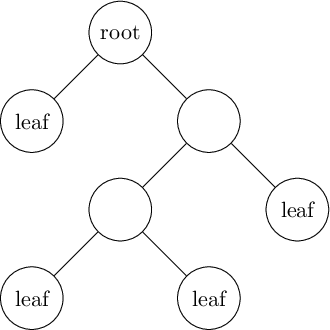
\includegraphics[width=0.4\textwidth]{xcas-tree.png}
\end{center}
which looks like an upside-down tree; the root is at the
top and the leaves are at the bottom.

Given an expression, the nodes of the corresponding
tree\index{expression tree} are the functions, operators, variables
and constants.  The children of a function node are its arguments, the
children of an operator node are its operands, and the constants and
variables will be the leaves.  For example, the tree for $\sin(2*x +
y)$ will look like
\begin{center}
  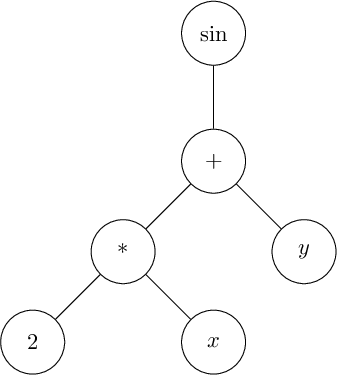
\includegraphics[width=0.4\textwidth]{xcas-expr-tree.png}
\end{center}
A subexpression\index{subexpression} of an expression will be a
selected node together with the nodes below it.  For example, both
$2*x$ and $2*x+y$ are subexpressions of $\sin(2*x+y)$, but $x+y$ is
not.

A subexpression of the contents of the expression editor can be
selected with the mouse; the selection will appear white on a black
background.  A subexpression can also be chosen with the keyboard
using the arrow keys.  Given a selection:
\begin{itemize}
  \item
  The up arrow will go to the parent node.
  \item
  The down arrow will go to the leftmost child node.
  \item
  The right and left arrows will go to the right and left sibling nodes.
  \item
  The control key with the right and left arrows will switch the
  selection with the corresponding sibling.
  \item
  If a constant or variable is selected, the backspace key will delete
  it.  For other selections, backspace will delete the function or
  operator, and another backspace will delete the arguments or operands.
\end{itemize}

You can use the arrow keys to navigate the tree structure of an
expression, which isn't always evident by looking at the expression
itself.  For example, suppose you enter \texttt{x*y*z} in the editor.
The two multiplications will be a different levels; the tree will look
like
\begin{center}
  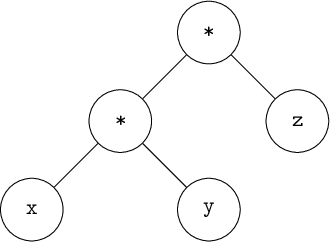
\includegraphics[width=0.4\textwidth]{xcas-xyz-tree.png}
\end{center}
If you select the entire expression with the up arrow and then go to
the \texttt{M} menu to the right of the line and choose eval, then the
expression will look the same but, as you can check by navigating it
with the arrow keys, the tree will look like
\begin{center}
  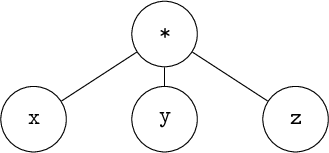
\includegraphics[width=0.4\textwidth]{xcas-xyz-tree2.png}
\end{center}

\subsection{Manipulating subexpressions\index{subexpressions}}

If a subexpression is selected in the expression editor, then any menu
command will be applied to that subexpression.

For example, suppose that you enter the expression
\begin{center}
  \texttt{(x+1)*(x+2)*(x-1)}
\end{center}
in the expression editor.  Note that you can use the abilities of the
editor to make this easier.  First, enter \texttt{x+1}.  Select this
with the up arrow, then type \texttt{*} followed by \texttt{x+2}.  Select
the \texttt{x+2} with the up arrow and then type \texttt{*} followed
by \texttt{x-1}.  Using the up arrow again will select the \texttt{x-1}.
Select the entire expression with the up arrow, and then select
\texttt{eval} from the \texttt{M} menu.  This will put all factors at
the same level.  Suppose you want the factors \texttt{(x+1)*(x+2)} to
be expanded.  You could select \texttt{(x+1)*(x+2)} with the mouse and
do one of the following:
\begin{itemize}
  \item
  Select the
  \texttt{Expression$\blacktriangleright$Misc$\blacktriangleright$normal}
  menu item.  You will then have \texttt{normal((x+1)*(x+2))*(x-1)} in
  the editor.  If you hit enter, the result $(x^2 + 3x + 2)*(x-1)$ will
  appear in the output window.
  \item
  Select the
  \texttt{Expression$\blacktriangleright$Misc$\blacktriangleright$normal}
  menu item, so again you have \texttt{normal((x+1)*(x+2))*(x-1)} in
  the editor.  Now if you select \texttt{eval} from the \texttt{M}
  menu, then the expression in the editor will become the result
  $(x^2 + 3x + 2)*(x-1)$, which you can continue editing.
  \item
  Choose \texttt{normal} from the \texttt{M} menu.  This will apply
  normal to the selection, and again you will have the result
  $(x^2 + 3x + 2)*(x-1)$ in the editor.
\end{itemize}

There are also keystroke commands that you can use to operate on
subexpressions that you've selected.  There are the usual
\texttt{Ctrl+Z} and \texttt{Ctrl+Y} for undoing and redoing.  Some of
the others are given in the following table.
\begin{center}
\begin{tabular}{|p{.20\textwidth}|p{.6\textwidth}|}
\hline
\textbf{Key} & \textbf{Action on selection}\\
%\multicolumn{2}{|c|}{\textbf{Conversions}}\\
\hline\hline
\texttt{Ctrl+D} & differentiate\\
\texttt{Ctrl+F} & factor\\
\texttt{Ctrl+L} & limit\\
\texttt{Ctrl+N} & normalize\\
\texttt{Ctrl+P} & partial fraction\\
\texttt{Ctrl+R} & integrate\\
\texttt{Ctrl+S} & simplify\\
\texttt{Ctrl+T} & copy \LaTeX{} version to clipboard\\
\hline
\end{tabular}
\end{center}

\section{Previous results: \texttt{ans} \index{ans}}

The \texttt{ans} command returns the results of previous commands.
\begin{itemize}
\item \texttt{ans} takes one optionaly argument:\\
Optionally, $n$, an integer (the number of the command beginning with 0).
\item \texttt{ans($\langle n\rangle $)} returns the corresponding
result; in particular, \texttt{ans(-1)} returns the previous result.
\end{itemize}

\smallskip

\noindent
\textbf{Example.}\\
If the first command that you enter is:\\
\textit{Input:}
\begin{center}
  \texttt{2+5}
\end{center}
resulting in\\
\textit{Output:}
\[
7
\]
%\begin{center}
%  \texttt{7}
%\end{center}
then later references to \texttt{ans(0)} will evaluate to \texttt{7}.

\smallskip

Note that the argument to \texttt{ans} doesn't correspond to the line
number in \texttt{Xcas}.  For one thing, the line numbers begin at 1.
What's more, if you go back and re-evaluate a previous line, then that
will become part of the commands that \texttt{ans} keeps track of.

If you give \texttt{ans} a negative number, then it counts backwards
from the current input.  To get the latest output, for example, you
can use \texttt{ans(-1)}.  With no argument, \texttt{ans()} will also
return the latest output.

Similarly, the \texttt{quest\index{quest}} command returns the
previous inputs.  Since these will often be simplified to be the same
as the output, \texttt{quest($n$)} sometimes has the same value as
\texttt{ans($n$)}.

You can also use \texttt{Ctrl} plus the arrow keys to scroll through
previous inputs.  With the cursor on the command line,
\texttt{Ctrl+uparrow} will go backwards in the list of previous
commands and display them on the current line, and
\texttt{Ctrl+downarrow} will go forwards.

\section{Spreadsheet\label{sec:spreadsheet}\index{spreadsheet}}

\subsection{Opening a spreadsheet}

You can open a spreadsheet (or a matrix editor) with the
\texttt{Spreadsheet$\blacktriangleright$New Spreadsheet} menu item or
with the key \texttt{Alt+T}.

When you open a new spreadsheet, you will be given a configuration
screen with the following options:
\begin{itemize}
  \item
  \texttt{Variable}
  This has a input field where you can type in a variable name; the
  spreadsheet will be saved as a matrix in this variable.
  \item
  \texttt{Rows} and \texttt{Columns}
  These have input fields where you can type in positive integers
  specifying the number of rows and columns in the spreadsheet.
  \item
  \texttt{Eval}
  This has a checkbox.  If the box is checked, then the
  spreadsheet will be re-evaluated every time you make a change to it.
  If it is not checked, it won't be re-evaluated when changes are
  made, but you can still re-evaluate the spreadsheet
  with the \texttt{eval} button on the spreadsheet menu bar.
  \item
  \texttt{Distribute}
  This has a checkbox.  If it is checked, then entering a matrix
  will distribute the contents across an appropriate array of cells.
  If it is not checked, then the matrix will be put in one cell.
  \item
  \texttt{Landscape}
  This has a checkbox.  If it is checked, then
  the graphical representation of the spreadsheet will be displayed
  below the spreadsheet.  If it is not checked, then it will be
  displayed to the right of the spreadsheet.
  \item
  \texttt{Move right}
  This has a checkbox.  If it is checked, then the cursor will move
  to the cell to the right of the current cell
  when data is entered.  If this is not checked, the cursor will be moved to
  the cell below the current cell.
  \item
  \texttt{Spreadsheet}
  This has a checkbox.  If it is checked, the spreadsheet will be
  formatted as a spreadsheet.  If it is not checked, it will be
  formatted as a matrix.
  \item
  \texttt{Graph}
  This has a checkbox.  If it is checked, the graphical representation of the
  spreadsheet will be displayed.  If it is not checked, the graphical
  representation will not be displayed.
  \item
  \texttt{Undo history}
  This has an input field where you can type in a postive integer,
  specifying how many undo's can be performed at a time.
  % \item
  % \texttt{Init sheet}
\end{itemize}
The configuration screen can be reopened with the
\texttt{Edit$\blacktriangleright$Configuration$\blacktriangleright$Cfg
window} menu attached to the spreadsheet.

\subsection{The spreadsheet window}

When you open a spreadsheet, the input line will become the
spreadsheet.
\begin{center}
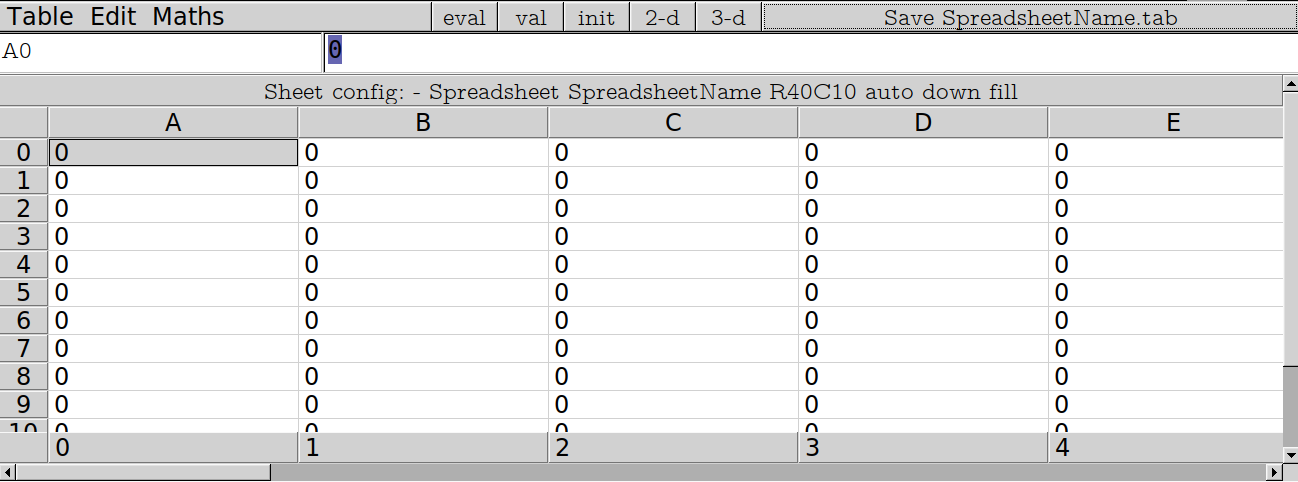
\includegraphics[width=0.75\textwidth]{xcas-spreadsheet.png}
\end{center}
The top will be a menu bar with
\texttt{Table}, \texttt{Edit} and \texttt{Maths} menus as well as
\texttt{eval}, \texttt{val}, \texttt{init}, \texttt{2-d} and
\texttt{3-d} buttons.
%% More info on the menus?
To the right will be the name of the file the spreadsheet will be
saved into. Below the menu bar will be two boxes; a box which displays
the active cell (and can be used to choose a cell) and a command line
to enter information into the cell. Below that will be a status line,
you can click on this to return to the configuration screen.

\chapter{CAS building blocks\label{chap:casbb}}

\section{Numbers\label{sec:numbs}}

\texttt{Xcas} works with both real and complex numbers.  The real
numbers can be integers, rational numbers, floating point numbers or
symbolic constants.

You can enter an integer by simply typing the digits.\\
\textit{Input:}
\begin{center}
  \texttt{1234321}
\end{center}
\textit{Output:}
\[
1234321
\]
% \begin{center}
%   \texttt{1234321}
% \end{center}
Alternatively, you can enter an integer in binary (base 2) by
prefixing the digits (0 through 1) with \texttt{0b}, in octal (base 8)
by prefixing the digits (0 through 7) with \texttt{0} or \texttt{0o},
and in hexadecimal (base 16) by prefixing the digits (0 through 9 and
a through f) with \texttt{0x}.  (See \secref{ssec:binocthex}.)\\
\texttt{Input:}
\begin{center}
  \texttt{0xab12}
\end{center}
Output:
\[
43794
\]
% \begin{center}
%   \texttt{43794}
% \end{center}

You can enter a rational number as the ratio of two integers.\\
\textit{Input:}
\begin{center}
  \texttt{123/45}
\end{center}
\textit{Output:}
\[
\frac{41}{15}
\]
% \begin{center}
%   \texttt{41/15}
% \end{center}
The result will be put in lowest terms.  If the top is a multiple of
the bottom, the result will be an integer.\\
\textit{Input:}
\begin{center}
  \texttt{123/3}
\end{center}
\textit{Output:}
\[
41
\]
% \begin{center}
%   \texttt{41}
% \end{center}

A floating point number is regarded as an approximation to a real
number.  You can enter a floating point number by writing it out with
a decimal point.\\
\textit{Input:}
\begin{center}
  \texttt{123.45}
\end{center}
\textit{Output:}
\[
123.45
\]
% \begin{center}
%   \texttt{123.45}
% \end{center}
You can also enter a floating point number by
entering a sequence of digits, with an optional decimal point,
followed by \texttt{e} and then an integer, where the \texttt{e}
represents ``times 10 to the following power.''\\
\textit{Input:}
\begin{center}
  \texttt{1234e3}
\end{center}
\textit{Output:}
\[
1234000.0
\]
% \begin{center}
%   \texttt{1234000.0}
% \end{center}
Floating point numbers with a large number of digits will be printed with
\texttt{e} notation; you can control how other floats are displayed
(see \secref{ssec:confcomp}, item \ref{enum:float}).
An integer or rational number can be converted to a floating point
number with \texttt{evalf} (see \secref{ssec:evalf}).

A complex number is a number of the form \texttt{$a$+$b$i}, where $a$
and $b$ are real numbers.  The numbers $a$ and $b$ will be the same
type of real number; one type will be converted to the other type if
necessary (an integer can be converted to a rational number or a
floating point number, and a rational number can be converted to a
floating point number).\\
\textit{Input:}
\begin{center}
  \texttt{3 + 1.1i}
\end{center}
\textit{Output:}
\[
3+1.1i
\]
% \begin{center}
%   \texttt{3.0+1.1i}
% \end{center}

\section{Symbolic constants: \texttt{e} \texttt{pi} \texttt{infinity}
\texttt{inf} \texttt{i} \texttt{euler\_gamma} \index{e} \index{pi}
\index{infinity} \index{inf} \index{i} \index{euler\_gamma}
\index{\%e} \index{\%pi} \index{\%i} \index{+infinity}
\index{-infinity} \index{-inf}}

\texttt{Xcas} has the standard constants given by built-in symbols,
given in the following table.
\begin{center}
\begin{tabular}{|p{.3\textwidth}|p{.4\textwidth}|}
\hline
\textbf{Symbol} & \textbf{Value}\\
\hline\hline
\texttt{e} (or \texttt{\%e}) & the number $\exp(1)$\\
\texttt{pi} (or \texttt{\%pi}) & the number $\pi$\\
\texttt{infinity} & unsigned $\infty$\\
\texttt{+infinity} (or \texttt{inf}) & $+\infty$\\
\texttt{-infinity} (or \texttt{-inf}) & $-\infty$\\
\texttt{i} (or \texttt{\%i}) & the complex number $i$\\
\texttt{euler\_gamma} & Euler's constant $\gamma$; namely,
$\lim_{n\to\infty}\left(\sum_{k=1}^{n} - \ln(n)\right)$\\
\hline
\end{tabular}
\end{center}

% \texttt{e} (or \texttt{\%e}) is the number $\exp(1)$.\\
%\texttt{pi} (or \texttt{\%pi}) is the number $\pi$.\\
% \texttt{infinity} is unsigned $\infty$.\\
% \texttt{+infinity} (or \texttt{inf}) is $+\infty$.\\
% \texttt{-infinity} (or \texttt{-inf}) is $-\infty$.\\
% \texttt{i} (or \texttt{\%i}) is the complex number $i$.\\
% \texttt{euler\_gamma} is Euler's constant $\gamma$; namely,
% $\lim_{n\to\infty}\left(\sum_{k=1}^{n} - \ln(n)\right)$.

Since these numbers cannot be written exactly as standard decimal
numbers, they are necessarily left unevaluated in exact results (see
\secref{ssec:approx}).\\
\textit{Input:}
\begin{center}
  \texttt{2*pi}
\end{center}
\textit{Output:}
\[
2\pi
\]
% \begin{center}
%   \texttt{2*pi}
% \end{center}
\textit{Input:}
\begin{center}
  \texttt{2.0*pi}
\end{center}
\textit{Output:}
\[
6.28318530718
\]
% \begin{center}
%   \texttt{6.28318530718}
% \end{center}
You can also use \texttt{evalf} (see \secref{ssec:evalf}), for
example, to approximate one of the real-valued constants to as many
decimal places as you want.\\
\textit{Input:}
\begin{center}
  \texttt{evalf(pi,50)}
\end{center}
\textit{Output:}
\[
3.1415926535897932384626433832795028841971693993751
\]
% \begin{center}
%   \texttt{3.1415926535897932384626433832795028841971693993751}
% \end{center}

\section{Sequences, sets and lists\label{sec:seqlst}}

\subsection{Sequences: \texttt{seq[] ()}\index{seq[]}\index{()}\label{ssec:seqbasics}}

A sequence is represented by a sequence of elements separated by
commas, without delimiters or with either parentheses (\texttt{(} and
\texttt{)}) or \texttt{seq[} and \texttt{]} as delimiters, as in:\\
\textit{Input:}
\begin{center}
\texttt{1,2,3,4}
\end{center}
\textit{or:}
\begin{center}
\texttt{(1,2,3,4)}
\end{center}
\textit{or:}
\begin{center}
\texttt{seq[1,2,3,4]}
\end{center}
\textit{Output:}
\[
1,2,3,4
\]
% \begin{center}
% \texttt{1,2,3,4}
% \end{center}

Note that the order of the elements of a sequence is significant. For
example, if \texttt{B:=(5,6,3,4)} and \texttt{C:=(3,4,5,6)}, then
\texttt{B==C} returns \texttt{false}.\\
(A value can be assigned to a variable with the \texttt{:=} operator;
see \secref{ssec:varname}.
Also, \texttt{==} is the test for equality; see
\secref{ssec:booltests}.)

Note also that the expressions \texttt{seq[$\ldots$]} and
\texttt{seq($\ldots$)} are not the same (see \secref{ssec:makeseq} for
information on \texttt{seq($\ldots$)}). For example,
\texttt{seq([0,2])=(0,0)} and \texttt{seq([0,1,1,5])=[0,0,0,0,0]}
but\\
\texttt{seq[0,2]=(0,2)} and \texttt{seq[0,1,1,5]=(0,1,1,5)}

See \secref{sec:seq} for operations on sequences.

\subsection{Sets: \texttt{set[]}
\index{\%\{ \%\}}\index{set[]}\label{ssec:sets}}

To define a set of elements, put the elements separated by commas,
with delimiters \texttt{\%\{} and \texttt{\%\}} or \texttt{set[} and
\texttt{]}.\\
\textit{Input:}
\begin{center}
\texttt{set[1,2,3,4]}
\end{center}
\textit{or:}
\begin{center}
\texttt{\%\{1,2,3,4\%\}}
\end{center}
\textit{Output:}
\[
\leftsetbracket 1,2,3,4\rightsetbracket
\]
% \begin{center}
% \texttt{set[1,2,3,4]}
% \end{center}
In the \texttt{Xcas} output, the set delimiters are displayed
as $\leftsetbracket$ and $\rightsetbracket$ in order
%as $\llbracket$ and $\rrbracket$ in order
not to confuse sets with lists (see \secref{ssec:lstbasics}).
For example, \leftsetbracket 1,2,3 \rightsetbracket is the set \texttt{\%\{1,2,3\%\}},
unlike [1,2,3] (normal brackets) which is the list \texttt{[1,2,3]}.\\
\textit{Input:}
\begin{center}
    \texttt{A:=\%\{1,2,3,4\%\}}
\end{center}
\textit{or:}
\begin{center}
    \texttt{A:=set[1,2,3,4]}
\end{center}
\textit{Output:}
\[
\leftsetbracket 1,2,3,4\rightsetbracket
\]
% \begin{center}
%     \texttt{$\llbracket$1,2,3,4$\rrbracket$}
% \end{center}
\textit{Input:}
\begin{center}
   \texttt{B:=\%\{5,5,6,3,4\%\}}
\end{center}
\textit{or:}
\begin{center}
   \texttt{B:=set[5,5,6,3,4]}
\end{center}
\textit{Output:}
\[
     \leftsetbracket 5,6,3,4 \rightsetbracket
\]
% \begin{center}
%     \texttt{$\llbracket$5,6,3,4$\rrbracket$}
% \end{center}

\smallskip

\noindent
\textbf{Remark.}\\
The order in a set is not significant and the elements in a set are
all distinct. If you input \texttt{B:=\%\{5,5,6,3,4\%\}} and
\texttt{C:=\%\{3,4,5,3,6\%\}}, then \texttt{B==C} will return \texttt{true}.

See \secref{sec:setops} for operations on sets.

\subsection{Lists: \texttt{[ ]}\label{ssec:lstbasics}}

A list is delimited by \texttt{[} and \texttt{]}, its
elements must be separated by commas.  For example, \texttt{[1,2,5]}
is a list of three integers.  Lists are also called vectors in
\texttt{Xcas}.

Lists can contain lists (for example, a matrix is a list of lists of
the same size, see \secref{sec:defmat}). Lists may be used to
represent vectors (lists of coordinates), matrices, or univariate
polynomials (lists of coefficients by decreasing order, see
\secref{ssec:spoly}).

Lists are different from sequences, because sequences are flat: an
element of a sequence cannot be a sequence. Lists are different from
sets, because for a list, the order is important and the same element
can be repeated in a list (unlike in a set where each element is
unique).  See \secref{sec:lists} for operations on lists.

In \texttt{Xcas} output:
\begin{itemize}
\item list delimiters are displayed as $[$,$]$,
\item matrix delimiters are displayed as $[$,$]$
\item polynomial delimiters are displayed as $\leftpolybracket$,
$\rightpolybracket$
%$\talloblong \ \talloblong$,
\item set delimiters are displayed as $\leftsetbracket$,
$\rightsetbracket$.
%$\llbracket \ \rrbracket$.
\end{itemize}

\subsection{Accessing elements\label{ssec:els}}

The elements of sequences and lists are indexed starting from 0 in
Xcas syntax mode and from 1 in all other syntax modes (see
\secref{ssec:lang}).  To access an element of a list or a sequence,
follow the list with the index between square brackets.

\smallskip

\noindent
\textbf{Examples.}
\begin{itemize}
\item 
\textit{Input:}
\begin{center}
  \texttt{L:= [2,5,1,4]}
\end{center}
\textit{Output:}
\[
\left[2,5,1,4\right]
\]
%\begin{center}
%  \texttt{[2,5,1,4]}
%\end{center}
\item
\textit{Input:}
\begin{center}
  \texttt{L[1]}
\end{center}
\textit{Output:}
\[
5
\]
% \begin{center}
%   \texttt{5}
% \end{center}
\item
To access the last element of a list or sequence, you can put \texttt{-1} between
square brackets.\\
\textit{Input:}
\begin{center}
  \texttt{L[-1]}
\end{center}
\textit{Output:}
\[
4
\]
% \begin{center}
%   \texttt{4}
% \end{center}
\end{itemize}

If you want the indices to start from 1 in Xcas syntax mode, you can
enter the index between double brackets.

\smallskip

\noindent
\textbf{Example.}\\
\textit{Input:}
\begin{center}
  \texttt{L[[1]]}
\end{center}
\textit{Output:}
\[
2
\]
% \begin{center}
%   \texttt{2}
% \end{center}

\section{Variables\label{sec:vars}}

\subsection{Variable names\label{ssec:varname}}

A variable\index{variable} or function name is a sequence of letters,
numbers and underscores that begins with a letter.  If you define your
own variable or function, you can't use the names of built-in
variables or functions or other keywords reserved by \texttt{Xcas}.

\subsection{Assigning values: \texttt{:=} \texttt{=>} \texttt{=} \texttt{assign} \texttt{sto} \texttt{Store}
\index{:=}
\index{=>}
\index{=}
\index{assign}
\index{sto}
\index{Store}
\label{ssec:assign}}

You can assign a value to a variable with the \texttt{:=} operator.
For example, to give the variable \texttt{a} the value of \texttt{4},
you can enter
\begin{center}
  \texttt{a:= 4}
\end{center}
Alternatively, you can use the \texttt{=>} operator; when
you use this operator, the value comes before the variable;
\begin{center}
  \texttt{4 => a}
\end{center}
The function \texttt{sto} (or \texttt{Store})
can also be used; again, the value comes before the variable
(the value is stored into the variable);
\begin{center}
  \texttt{sto(4,a)}
\end{center}
After any one of these commands, whenever you use the variable
\texttt{a} in an expression, it will be replaced by \texttt{4}.

You can use sequences or lists to make multiple assignments at the
same time. For example,
\begin{center}
\texttt{(a,b,c):= (1,2,3)}
\end{center}
will assign \texttt{a} the value \texttt{1}, \texttt{b} the value
\texttt{2} and \texttt{c} the value \texttt{3}.   Note that this can
be used to switch the values of two variables; with \texttt{a} and
\texttt{b} as above, the command
\begin{center}
\texttt{(a,b):= (b,a)}
\end{center}
will set \texttt{a} equal to \texttt{b}'s original value, namely
\texttt{2}, and will set \texttt{b} equal to \texttt{a}'s original
value, namely \texttt{1}.

Another way to assign values to variables, useful in Maple mode, is
with the \texttt{assign} command. If you enter
\begin{center}
  \texttt{assign(a,3)}
\end{center}
or
\begin{center}
  \texttt{assign(a = 3)}
\end{center}
then \texttt{a} will have the value \texttt{3}.  You can assign
multiple values at once; if you enter
\begin{center}
  \texttt{assign([a = 1, b = 2])}
\end{center}
then \texttt{a} will have the value \texttt{1} and \texttt{b} will
have the value \texttt{2}.  This command can be useful in Maple mode,
where solutions of equations are returned as equations.  For example,
if you enter (in Maple mode)
\begin{center}
  \texttt{sol:= solve([x + y = 1, y = 2],[x,y])}
\end{center}
(see \secref{ssec:solve}) you will get
\[
[x=-1,y=2]
\]
%\begin{center}
%  \texttt{[x = -1, y = 2]}
%\end{center}
If you then enter
\begin{center}
  \texttt{assign(sol)}
\end{center}
the variable \texttt{x} will have value \texttt{-1} and \texttt{y}
will have the value \texttt{2}.  This same effect can be achieved in
standard \texttt{Xcas} mode, where
\begin{center}
  \texttt{sol:= solve([x + y = 1, y = 2],[x,y])}
\end{center}
will return
\[
\left[\left[-1,2\right]\right]
\]
%\begin{center}
%  \texttt{[[x = -1, y = 2]]}
%\end{center}
In this case, the command
\begin{center}
  \texttt{[x,y]:= sol[0]}
\end{center}
will assign \texttt{x} the value \texttt{-1} and \texttt{y} the value
\texttt{2}.

\subsection{Assignment by reference: \texttt{=<}
\index{=<}
\label{ssec:refassign}}

A list is simply a sequence of values separated by commas and
delimited by \texttt{[} and \texttt{]} (see \secref{sec:seq}). Suppose
you give the variable \texttt{a} the value \texttt{[1,1,3,4,5]},
\begin{center}
 \texttt{a:= [1,1,3,4,5]}
\end{center}
If you later assign to \texttt{a} the value \texttt{[1,2,3,4,5]}, then
a new list is created.  It may be better to just change the second
value in the original list by reference.  This can be done with the
\texttt{=<} command.  Recalling that lists are indexed beginning at 0,
the command
\begin{center}
  \texttt{a[1] =< 2}
\end{center}
will simply change the value of the second element of the list instead
of creating a new list, and is a more efficient way to change the
value of \texttt{a} to \texttt{[1,2,3,4,5]}.

\subsection{Copying lists: \texttt{copy}
\index{copy}
\label{ssec:copy}}

If you enter
\begin{center}
  \texttt{list1:= [1,2,3]}
\end{center}
and then
\begin{center}
  \texttt{list2:= list1}
\end{center}
then \texttt{list1} and \texttt{list2} will be equal to the same list,
not simply two lists with the same elements.  In particular, if you
change (by reference) the value of an element of \texttt{list1}, then
the change will also be reflected in \texttt{list2}.  For example, if
you enter
\begin{center}
  \texttt{list1[1] =< 5}
\end{center}
then both \texttt{list1} and \texttt{list2} will be equal to
\texttt{[1,5,3]}.

The \texttt{copy} command creates a copy of a list (or vector or
matrix) which is equal to the original list, but distinct from it. For
example, if you enter
\begin{center}
  \texttt{list1:= [1,2,3]}
\end{center}
and then
\begin{center}
  \texttt{list2:= copy(list1)}
\end{center}
then \texttt{list1} and \texttt{list2} will both be \texttt{[1,2,3]},
but now if you enter
\begin{center}
  \texttt{list1[1] =< 5}
\end{center}
then \texttt{list1} will be equal to \texttt{[1,5,3]} but
\texttt{list2} will still be \texttt{[1,2,3]}.

\subsection{Incrementing variables: \texttt{+=} \texttt{-=} \texttt{*=} \texttt{/=}
\index{+=}
\index{-=}
\index{*=}
\index{/=}}

You can increase the value of a variable \texttt{a} by \texttt{4}, for
example, with
\begin{center}
  \texttt{a:= a + 4}
\end{center}
If beforehand \texttt{a} were equal to \texttt{4}, it would now be
equal to \texttt{8}.  A shorthand way of doing this is with the
\texttt{+=}\index{+=} operator;
\begin{center}
  \texttt{a += 4}
\end{center}
will also increase the value of \texttt{a} by \texttt{4}.

Similar shorthands exist for subtraction, multiplication and division.
If \texttt{a} is equal to \texttt{8} and you enter
\begin{center}
  \texttt{a -= 2}
\end{center}
then \texttt{a} will be equal to \texttt{6}.  If you follow this with
\begin{center}
  \texttt{a *= 3}
\end{center}
then \texttt{a} will be equal to \texttt{18}, and finally
\begin{center}
  \texttt{a /= 9}
\end{center}
will end with \texttt{a} equal to \texttt{2}.


\subsection{Storing and recalling variables and their values: \texttt{archive}  \texttt{unarchive}
\index{archive}
\index{unarchive}}

The \texttt{archive} command stores the values of variables for later
use in a file of your choosing.
\begin{itemize}
\item \texttt{archive} takes two arguments:
\begin{itemize}
  \item \textit{filename}, a filename in which to store values.
  \item \textit{vars}, a variable or list of variables.
\end{itemize}
\item \texttt{archive("}\textit{filename}\texttt{",}\textit{vars}\texttt{)}
saves the values of \textit{vars} (or the values of the variables in
the list) in file \textit{filename}.
\end{itemize}
For example, if the variable \texttt{a} has the value \texttt{2} and the variable
\texttt{bee} has the value \texttt{"letter"} (a string), then entering
\begin{center}
  \texttt{archive("foo",[a,bee])}
\end{center}
will create a file named ``\texttt{foo}'' which contains the values
\texttt{2} and \texttt{"letter"} in a format meant to be efficiently
read by \texttt{Xcas}.

The \texttt{unarchive} command will read the values from a file
created with \texttt{archive}.
\begin{itemize}
\item \texttt{unarchive} takes one argument:\\
\textit{filename}, the filename.
\item \texttt{unarchive("}\textit{filename}\texttt{")} returns the value
or list of values stored in \textit{filename}.
\end{itemize}

\smallskip

\noindent
\textbf{Example.}\\
With the file ``\texttt{foo}'' as above:\\
\textit{Input:}
\begin{center}
  \texttt{unarchive("foo")}
\end{center}
\textit{Output:}
\[
\left[2,\text{"letter"}\right]
\]
% \begin{center}
%   \texttt{[2, letter]}
% \end{center}
If you want to reassign these values to \texttt{a} and \texttt{bee},
you can enter
\begin{center}
  \texttt{[a,bee]:= unarchive("foo")}
\end{center}

\subsection{Copying variables: \texttt{CopyVar}
\index{CopyVar}
\label{ssec:copyvar}}

The \texttt{CopyVar} command copies the contents of one variable into
another, without evaluating the contents.
\begin{itemize}
\item
\texttt{CopyVar} takes two arguments:
\begin{itemize}
  \item \textit{fromvar}, the name of a variable to copy from.
  \item \textit{tovar}, the name of a variable to copy to.
\end{itemize}
\item
\texttt{CopyVar(}\textit{fromvar}\texttt{,}\textit{tovar}\texttt{)}
copies the unevaluated contents of \textit{fromvar} into \texttt{tovar}.
\end{itemize}

\smallskip

\noindent
\textbf{Example.}\\
\textit{Input:}
\begin{center}
  \begin{tabular}{l}
    \texttt{a:=c} \\
    \texttt{c:=5}\\
    \texttt{CopyVar(a,b)}
  \end{tabular}
\end{center}
\textit{Output:}
\[
c
\]
\textit{then:}
\begin{center}
  \texttt{b}
\end{center}
\textit{Output:}
\[
5
\]
Changing the value if \texttt{c} will also change the output of
\texttt{b}, since \texttt{b} contains  \texttt{c}.\\
\textit{Input:}
\begin{center}
  \begin{tabular}{l}
    \texttt{c:=10:;}\\
    \texttt{b}
  \end{tabular}
\end{center}
\textit{Output:}
\[
10
\]

\subsection{Assumptions on variables: \texttt{about} \texttt{additionally} \texttt{assume} \texttt{purge} \texttt{supposons} \texttt{and} \texttt{or}
\index{about}
\index{additionally}
\index{assume}
\index{purge}
\index{supposons}
\index{and}
\index{or}
\label{ssec:about}}

If \texttt{variable} is a purely symbolic variable (i.e., it doesn't
have a value or any assumptions made about it), then
\begin{center}
  \texttt{abs(variable)}
\end{center}
will return
%Output
\[
\left|\mathrm{variable}\right|
\]
% \begin{center}
%   \texttt{abs(var)}
% \end{center}
since \texttt{Xcas} doesn't know what type of value the
variable is supposed to represent.

The \texttt{assume} (or \texttt{supposons}) command lets you tell
\texttt{Xcas} some properties of a variable without giving the
variable a specific value.  The \texttt{additionally} command can be
used to add assumptions to a variable.  The \texttt{about} command
will display the current assumptions about a variable, and the
\texttt{purge} command will remove all values and assumptions about a
variable.

\smallskip

\noindent
\texttt{assume} (or \texttt{supposons}) takes one mandatory
argument and one optional argument:
\begin{itemize}
  \item \textit{assumptions}, statements about a variable (such as
  equalities and inequalities, possibly combined with \texttt{and} and
  \texttt{or}, and domains).
  \item Optionally, \texttt{additionally}, which indicates that the
  assumptions are to be added to previous assumptions, as opposed to
  replace them.
\end{itemize}
\texttt{assume(}\textit{assumptions}$\,\langle$\texttt{,additionally}$\rangle$\texttt{)}
places the assumptions on the variable.  With no second argument,
it will remove any previous assumptions.

\smallskip

\begin{itemize}
\item
\texttt{additionally} takes one argument:\\
\textit{assumptions} as above.
\item
\texttt{additionally(}\textit{assumptions}\texttt{)} adds the
assumptions to a variable without removing assumptions.
\end{itemize}

\smallskip

\begin{itemize}
\item
\texttt{about} takes one argument:\\
\textit{var}, the name of a variable.
\item
\texttt{about(}\textit{var}\texttt{)} returns the current assumptions
on the variable.
\end{itemize}

\smallskip

\begin{itemize}
\item
\texttt{purge} takes one argument:\\
\textit{var}, a variable name or a sequence of variable names.
\item
\texttt{purge(}\textit{var}\texttt{)} removes any assumptions you have
made about the variable \textit{var} (or about all the variables in
the sequence).
\end{itemize}

\smallskip

For example, if you enter
\begin{center}
  \texttt{assume(variable > 0)}
\end{center}
then \texttt{Xcas} will assume that \texttt{variable} is a positive real
number, and so
\begin{center}
  \texttt{abs(variable)}
\end{center}
will be evaluated to
\[
\mathrm{variable}
\]
%\begin{center}
%   \texttt{var}
%\end{center}

You can put one or more conditions in the \texttt{assume} command by
combining them with \texttt{and} and \texttt{or}. For example, if you
want the variable \texttt{a} to be in $[2,4) \cup (6,\infty)$, you can
enter
\begin{center}
  \texttt{assume((a >= 2 and a < 4) or a > 6)}
\end{center}

If a variable has attached assumptions, then making another assumption
with \texttt{assume} will remove the original assumptions.  To add
extra assumptions, you can either use the \texttt{additionally}
command or give \texttt{assume} a second argument of
\texttt{additionally\index{additionally@\textit{additionally}}}.  If
you assume that $b > 0$ with
\begin{center}
  \texttt{assume(b > 0)}
\end{center}
and you want to add the condition that $b < 1$, you can either enter
\begin{center}
  \texttt{assume(b < 1, additionally)}
\end{center}
or
\begin{center}
  \texttt{additionally(b < 1)}
\end{center}

As well as equalities and inequalities, you can make assumptions about
the domain of a variable.  If you want \texttt{n} to represent an
integer\index{integer@\textit{integer}}, for example, you can enter
\begin{center}
  \texttt{assume(n, integer)}
\end{center}
If you want \texttt{n} to be a positive integer, you can add the
condition
\begin{center}
  \texttt{additionally(n > 0)}
\end{center}
You can also assume a variable is in one of the domains
\texttt{real}, \texttt{integer}, \texttt{complex} or
\texttt{rational} (see \secref{ssec:type}).

You can check the assumptions on a variable with the \texttt{about}
command. For the above positive integer \texttt{n},\\
\textit{Input:}
\begin{center}
  \texttt{about(n)}
\end{center}
\textit{Output:}
\begin{center}
  \texttt{assume[integer,[line[0,+infinity]],[0]]}
\end{center}
The first element tells you that \texttt{n} is an integer, the second
element tells you that \texttt{n} is between \texttt{0} and
\texttt{+infinity}, and the third element tells you that the value
\texttt{0} is excluded.

If you assume that a variable is equal to a specific value, such as
\begin{center}
  \texttt{assume(c = 2)}
\end{center}
then by default the variable \texttt{c} will remain unevaluated in
later levels.  If you want an expression involving \texttt{c} to be
evaluated, you would need to put the expression inside the
\texttt{evalf\index{evalf}} command (see \secref{ssec:evalf}).  After
the above assumption on \texttt{c}, if you enter
\begin{center}
  \texttt{evalf(c\^{}2 + 3)}
\end{center}
then you will get
\[
7.0
\]
%\begin{center}
%  \texttt{7.0}
%\end{center}
Right below the \texttt{assume(c = 2)} command line
there will be a slider; namely arrows pointing left and right with the
value \texttt{2} between them.  These
can be used to change the values of \texttt{c}.  If you click on the
right arrow, the \texttt{assume(c = 2)} command will transform to
\begin{center}
  \texttt{assume(c=[2.2,-10.0,10.0,0.0])}
\end{center}
and the value between the arrows will be \texttt{2.2}.  Also, any
later levels where the variable \texttt{c} is evaluated will be
re-evaluated with the value of \texttt{c} now \texttt{2.2}.  The
output to \texttt{evalf(c\^{}2 + 3} will become
\[
7.84
\]
%\begin{center}
%  \texttt{7.84}
%\end{center}
The \texttt{-10.0} and \texttt{10.0} in the \texttt{assume} line
represent the smallest and largest values that \texttt{c} can become
using the sliders.  You can set them yourself in the \texttt{assume}
command, as well as the increment that the value will change; if you
want \texttt{c} to start with the value \texttt{5} and vary between
\texttt{2} and \texttt{8} in increments of \texttt{0.05}, then you can
enter
\begin{center}
  \texttt{assume(c = [5,2,8,0.05])}
\end{center}

Recall the \texttt{purge} command removes assumptions about a
variable.\\
% \texttt{purge} takes a variable name \texttt{var} or a sequence of
% variable names.\\
% \texttt{purge(}\textit{var}\texttt{)} removes any
% assumptions you have made about the variable \textit{var} (or about
% all the variables in the sequence).\\
\textit{Input:}
\begin{center}
  \texttt{purge(a)}
\end{center}
then \texttt{a} will no longer have any assumptions made about it.\\
\textit{Input:}
\begin{center}
  \texttt{purge(a,b)}
\end{center}
then \texttt{a} and \texttt{b} will no longer have any assumptions
made about them.

\subsection{Unassigning variables: \texttt{VARS} \texttt{purge} \texttt{DelVar} \texttt{del} \texttt{restart} \texttt{rm\_a\_z} \texttt{rm\_all\_vars}
\index{VARS}
\index{purge}
\index{DelVar}
\index{del}
\index{restart}
\index{rm\_a\_z}
\index{rm\_all\_vars}
\label{ssec:VARS}}

\texttt{Xcas} has commands that help you keep track of what variables
you are using and resetting them if desired.  The \texttt{VARS}
command will list all the variables that you are using, the
\texttt{purge}, \texttt{DelVar} and \texttt{del} commands will delete
selected variables, and the \texttt{rm\_a\_z} and
\texttt{rm\_all\_vars} commands will remove classes of variables.

\begin{itemize}
\item
\texttt{VARS} takes no arguments.
\item
\texttt{VARS()} returns a list of the variables that you have assigned
values or made assumptions on.
\end{itemize}

\smallskip

\noindent
\textbf{Example.}\\
\textit{Input:}
\begin{center}
  \begin{tabular}{l}
  \texttt{a:= 1}\\
  \texttt{anothervar:= 2}
  \end{tabular}
\end{center}
\textit{then:}
\begin{center}
  \texttt{VARS()}
\end{center}
\textit{Output:}
\[
\left[a,\mathrm{anothervar}\right]
\]
%\begin{center}
%  \texttt{[a, anothervar]}
%\end{center}

\smallskip

The \texttt{purge} command will clear the values and assumptions you
make on variables (see \secref{ssec:about}).  For \texttt{TI}
compatibility there is also \texttt{DelVar}, and for Python
compatibility there is \texttt{del}.
\begin{itemize}
\item
The \texttt{purge} command takes one argument:\\
\textit{var}, the name of a variable.
\item
\texttt{purge(}\textit{var}\texttt{)} clears the variable \textit{var}
of all values and assumptions.
\end{itemize}

\begin{itemize}
\item
The \texttt{DelVar} (and \texttt{del}) commands take one argument:\\
\textit{var},  the name of a variable.
\item \texttt{Delvar} \textit{var} (or \texttt{del} \textit{var})
removes the values attached to \textit{var}.  (Note that
they do not take their argument in parentheses.
\end{itemize}

\smallskip

\noindent
\textbf{Example.}\\
To clear the variable \texttt{a}:\\
\textit{Input:}
\begin{center}
  \texttt{purge(a)}
\end{center}
\textit{or (for \texttt{TI} compatibility):}\\
\textit{Input:}
\begin{center}
  \texttt{DelVar a}
\end{center}
\textit{or (for Python compatibility):}\\
\textit{Input:}
\begin{center}
  \texttt{del a}
\end{center}

\smallskip

The \texttt{rm\_all\_vars} and \texttt{restart} commands clear the
values and assumptions you have made on all variables you can use.
\begin{itemize}
  \item \texttt{rm\_all\_vars} takes no arguments.
  \item \texttt{rm\_all\_vars()} removes all the values that you have
  attached to variables.
\end{itemize}

\smallskip

\begin{itemize}
  \item \texttt{restart} takes no arguments.
  \item \texttt{restart} removes all the values that you have
  attached to variables.  (Note that it does not use parentheses.)
\end{itemize}

\smallskip

The \texttt{rm\_a\_z} command clears the values and assumptions on all
variables with single lowercase letter names.
\begin{itemize}
  \item \texttt{rm\_a\_z} takes no arguments.
  \item \texttt{rm\_a\_z()}  purges all variables whose names are one letter
and lowercase.
\end{itemize}

\smallskip

\noindent
\textbf{Example.}\\
If you have variables names \texttt{A,B,a,b,myvar}, then after:\\
\textit{Input:}
\begin{center}
  \texttt{rm\_a\_z()}
\end{center}
you will only have the variables named \texttt{A,B,myvar}.

\subsection{The \texttt{CST} variable
\index{CST}
\label{ssec:CST}}

The menu available with the \texttt{cust} button in the bandeau on the
onscreen keyboard (see \secref{sec:swin}, item \ref{enum:kbd}) is
defined with the \texttt{CST} variable.  It is a list where each list
item determines a menu item; a list item is either a builtin command
name or a list itself consisting of a string to be displayed in the
menu and the input to be entered when the item is selected.

For example, to create a custom defined menu with the builtin function
\texttt{diff}, a user defined function \texttt{foo}, and a menu item
to insert the number $22/7$, you can:\\
\textit{Input:}
\begin{center}
  \texttt{CST:= [diff,["foo",foo],["My pi approx",22/7]]}
\end{center}

Note that if the input to be entered is a variable and the variable
has a value when \texttt{CST} is defined, then \texttt{CST} will
contain the value of the variable.  For example,\\
\textit{Input:}
\begin{center}
  \begin{tabular}{l}
  \texttt{app:= 22/7}\\
  \texttt{CST:= [diff,["foo",foo],["My pi approx",app]]}
  \end{tabular}
\end{center}
will be equivalent to the previous definition of \texttt{CST}.
However, if the variable does not have a value when \texttt{CST} is
defined, for example:\\
\textit{Input:}
\begin{center}
  \begin{tabular}{l}
  \texttt{CST:= [diff,["foo",foo],["My pi approx",app]]}\\
  \texttt{app:= 22/7}
  \end{tabular}
\end{center}
then \texttt{CST} will behave as the previous values to begin with,
but in this case if the variable \texttt{app} is changed, the
the result of pressing the \texttt{My pi approx} button will change
also.

Since \texttt{CST} is a list, a function can be added to the
\texttt{cust} menu with the \texttt{concat} command (see
\secref{ssec:concat});\\
\textit{Input:}
\begin{center}
  \texttt{CST:= concat(CST,evalc)}
\end{center}
will add the \texttt{evalc} command to the \texttt{cust} menu.

\section{Functions}

\subsection{Defining functions\label{ssec:deffuns}}

Similar to how you can assign a value to a variable (see
\secref{ssec:assign}), you can use the \texttt{:=}\index{:=} and
\texttt{=>}\index{=>} operators to define a function; both
\begin{center}
  \texttt{f(x):= x\^{}2}
\end{center}
and
\begin{center}
  \texttt{x\^{}2 => f(x)}
\end{center}
give the name \texttt{f} to the function which takes a value and
returns the square of the value.  In either case, if you then enter:\\
\textit{Input:}
\begin{center}
  \texttt{f(3)}
\end{center}
you will get:\\
\textit{Output:}
\[
9
\]
%\begin{center}
%  \texttt{9}
%\end{center}

You can define an anonymous function, namely a function without a
name, with the \texttt{->}\index{->} operator; the squaring function
can be written
\begin{center}
  \texttt{x -> x\^{}2}
\end{center}
You can use this form of the function to assign it a name; both
\begin{center}
  \texttt{f:= x -> x\^{}2}
\end{center}
and
\begin{center}
  \texttt{x -> x\^{}2 => f}
\end{center}
are alternate ways to define \texttt{f} as the squaring function.

You can similarly define functions of more than one variable.  For
example, to define a function which takes the lengths of the two legs
of a right triangle and returns the hypotenuse, you could enter
\begin{center}
  \texttt{hypot(a,b):= sqrt(a\^{}2 + b\^{}2)}
\end{center}
or
\begin{center}
  \texttt{hypot:= (a,b) -> sqrt(a\^{}2 + b\^{}2)}
\end{center}

\section{Directories\index{directories}}

\subsection{Working directories: \texttt{pwd} \texttt{cd}
\index{pwd}
\index{cd}
\label{ssec:wdir}}

\texttt{Xcas} has a working directory where it stores files that it
creates; typically this is the user's home directory. The \texttt{pwd}
command will tell you what the current working directory is, and and
the \texttt{cd} command lets you change it.

\begin{itemize}
\item \texttt{pwd} takes no arguments.
\item \texttt{pwd()} returns the name of the current working directory.
\end{itemize}

\smallskip

\noindent
\textbf{Example.}\\
\textit{Input:}
\begin{center}
  \texttt{pwd()}
\end{center}
\textit{Output:} might be something like:
\begin{center}
  \texttt{/home/username}
\end{center}

\smallskip

\begin{itemize}
\item The \texttt{cd} command takes one argument:\\
\textit{dirname}, the name of a directory (a string).
\item \texttt{cd(}\textit{dirname}\texttt{)} changes the working directory to
\textit{dirname}.
\end{itemize}

\smallskip

\noindent
\textbf{Example.}\\
If you enter:\\
\textit{Input:}
\begin{center}
  \texttt{cd("foo")}
\end{center}
or (on a Unix system):\\
\textit{Input:}
\begin{center}
  \texttt{cd("/home/username/foo")}
\end{center}
then the working directory will change to the directory \texttt{foo},
if it exists. Afterwards, any files that you save from \texttt{Xcas}
will be in that directory.

\smallskip

To load or read a file, it will need to be in the working directory.
Note that if you have the same file name in different directories,
then loading the file name will load the file in the current
directory.

\subsection{Reading files: \texttt{read} \texttt{load}
\index{read}
\index{load}
\label{ssec:read}}

Information for \texttt{Xcas} can be stored in a file; this
information can be read with the \texttt{read} or \texttt{load}
command, depending on the type of information.

\medskip

The \texttt{read} command reads a file containing \texttt{Xcas}
information, such as a program that you saved (see
\secref{ssec:progsave}) or simply commands that you typed into a file
with a text editor.  The file should have the suffix \texttt{.cxx}.
\begin{itemize}
\item
\texttt{read} takes one argument:\\
\textit{filename}, the name of a file (a string) containing a saved program (see
\secref{ssec:progsave}) or other commands.
\item
\texttt{read(}\textit{filename}\texttt{)} reads the content of
the file.
\end{itemize}

\smallskip

\noindent
\textbf{Example.}\\
If you have a file named \texttt{myfunction.cxx},\\
\textit{Input:}
\begin{center}
  \texttt{read("myfunction.cxx")}
\end{center}
will read in the file, as long as the directory is in the current working
directory.  If the file is in a different directory, you can still
read it by giving the path to the file,\\
\textit{Input:}
\begin{center}
  \texttt{read("/path/to/file/myfunction.cxx")}
\end{center}

\medskip

The \texttt{load} command reads in a saved session (see
\secref{ssec:sesssave}), which will end in \texttt{.xws}.
\begin{itemize}
\item
\texttt{load} takes one argument:\\
\textit{filename}, the name of a file (a string) containing a saved session.
\item
\texttt{load(}\textit{filename}\texttt{)} loads the session stored in
\textit{filename}.
\end{itemize}

\smallskip

\noindent
\textbf{Example.}\\
If you have a session saved in the file \texttt{mysession.xws},\\
\textit{Input:}
\begin{center}
  \texttt{load("mysession.xws")}
\end{center}
loads \texttt{mysession.xws}.

\subsection{Internal directories: \texttt{NewFold} \texttt{SetFold} \texttt{GetFold} \texttt{DelFold} \texttt{VARS}
\index{NewFold}
\index{SetFold}
\index{GetFold}
\index{DelFold}
\index{VARS}
\index{internal directories}}

You can create a directory that isn't actually on your hard drive but
is treated like one by \texttt{Xcas} with the command
\texttt{NewFold}.
\begin{itemize}
\item
\texttt{NewFold} takes one argument:
\textit{MyIntDir}, a variable name (see \secref{ssec:varname}).
\item
\texttt{NewFold(}\textit{MyIntDir}\textit{)}
creates a new internal directory named \textit{MyIntDir}.
(Note that quotation marks are not used.)
\end{itemize}

Internal directories will be listed with the \texttt{VARS()} command
(see \secref{ssec:VARS}).

To actually use this directory, you'll have to use the
\texttt{SetFold} command.
\begin{itemize}
\item
The \texttt{SetFold} command takes one argument:\\
\textit{MyIntDir}, the variable name  of an internal directory created with
\texttt{NewFold}.
\item
\texttt{SetFold(}\textit{MyIntDir}\texttt{)}
makes \textit{MyIntDir} the working directory (see \secref{ssec:wdir}).
\end{itemize}

Finally, you can print out the internal directory that you are in with
the \texttt{GetFold} command.
\begin{itemize}
  \item \texttt{GetFold} takes no arguments.
  \item \texttt{GetFold()} returns the name of the current internal
  directory.
\end{itemize}

\smallskip

\noindent
\textbf{Example.}\\
\textit{Input:}
\begin{center}
  \texttt{GetFold()}
\end{center}
will display the current internal directory.

\smallskip

\noindent
The \texttt{DelFold} command will delete an internal directory.
\begin{itemize}
\item
\texttt{DelFold} takes one argument:\\
\textit{MyIntDir}, the variable name of an internal directory.
\item
\texttt{DelFold(}\textit{MyIntDir}\texttt{)} will delete the directory
if it is empty.
\end{itemize}

\chapter{The CAS functions\label{chap:cas}}

\section{Booleans\label{sec:boolean}}

\subsection{Boolean values: \texttt{true} \texttt{false}
\index{true}
\index{false}
\index{TRUE}
\index{FALSE}
\index{boolean}}

The symbols \texttt{true} and \texttt{false} are \textit{booleans},
and are meant to indicate a statement is true or false.

These constants have synonyms:
\begin{itemize}
  \item \texttt{true} is the same as \texttt{TRUE} or \texttt{1}.
  \item \texttt{false} is the same as \texttt{FALSE} or \texttt{0}.
\end{itemize}

A function which returns a boolean is called a \emph{test} (or a
\emph{condition} or a \emph{boolean function}).

\subsection{Tests: \texttt{==} \texttt{!=} \texttt{>} \texttt{>=} \texttt{<} \texttt{=<}
\index{==}
\index{!=}
\index{>}
\index{>=}
\index{<}
\index{=<}
\label{ssec:booltests}}

The usual comparison operators between numbers are examples of tests.
In \texttt{Xcas}, they are the infixed operators:
\begin{description}
  \item[\texttt{==}]~\\
  \texttt{$a$==$b$} tests the equality
    between $a$ and $b$ and returns \texttt{1} if $a$
    is equal to $b$ and \texttt{0} otherwise.\\
    \textbf{Look out !}\\
    Note that \texttt{$a$=$b$}  is \textbf{not} a boolean!!!! This form is
    used to state that the expression \emph{is} an equality, perhaps with the
    intent to solve it.  To \emph{test} for equality, you need to use
    \texttt{$a$==$b$}, which
    \emph{is} a boolean.
  \item[\texttt{!=}]~\\
  \texttt{$a$!=$b$} returns \texttt{1} if $a$ and
    $b$ are different and \texttt{0} otherwise.
  \item[\texttt{>=}]~\\
  \texttt{$a$>=$b$} returns \texttt{1} if $a$
    is greater than or equal to $b$ and \texttt{0} otherwise.
  \item[\texttt{>}]~\\
  \texttt{$a$>$b$} returns \texttt{1} if $a$ is strictly
    greater than $b$ and \texttt{0} otherwise.
  \item[\texttt{<=}]~\\
  \texttt{$a$<=$b$} returns \texttt{1} if $a$ is less
    than or equal to $b$ and  \texttt{0} otherwise.
  \item[\texttt{<}]~\\
  \texttt{$a$<$b$} returns \texttt{1} if $a$
    is strictly less than $b$ and \texttt{0} otherwise.
\end{description}

\subsection{Defining functions with boolean tests: \texttt{ifte} \texttt{?:} \texttt{when}
\index{ifte}
\index{?:}
\index{when}
\index{piecewise defined functions}
\label{ssec:piecewise}}

You can use boolean tests to define functions not given by a single
simple formula.  Notably, you can use the \texttt{ifte} command or
\texttt{?:} operator to define piecewise-defined functions.
\begin{itemize}
  \item \texttt{ifte} takes three arguments:
  \begin{itemize}
    \item \textit{condition}, a boolean condition.
    \item \textit{true-result}, the result to return if
    \textit{condition} is true.
    \item \textit{false-result}, the result to return if
    \textit{condition} is false.
   \end{itemize}
   \item \texttt{ifte(}\textit{condition, true-result,
   false-result}\texttt{)} returns \textit{true-result} if
   \textit{condition} is true and returns \textit{false-result} if
   \textit{condition} if false.
\end{itemize}

\smallskip

\noindent
\textbf{Example.}\\
You can define your own absolute value function with:\\
\textit{Input:}
\begin{center}
  \texttt{myabs(x):= ifte(x >= 0, x, -1*x)}
\end{center}
Afterwards, entering:\\
\textit{Input:}
\begin{center}
  \texttt{myabs(-4)}
\end{center}
will return:
\[
4
\]
%\begin{center}
%  \texttt{4}
%\end{center}
However,  \texttt{myabs} will return an error if it can't evaluate the
condition.\\
\textit{Input:}
\begin{center}
  \texttt{myabs(x)}
\end{center}
\textit{Output:}
%Output:
\begin{center}
  \texttt{Ifte: Unable to check test Error: Bad Argument Value}
\end{center}

\smallskip

The \texttt{?:} construct behaves similarly to \texttt{ifte}, but is
structured differently and doesn't return an error if the condition
can't be evaluated.
\begin{itemize}
  \item The \texttt{?:} construct takes three arguments:
  \begin{itemize}
    \item \textit{condition}, a boolean condition.
    \item \textit{true-result}, the result to return if
    \textit{condition} is true.
    \item \textit{false-result}, the result to return if
    \textit{condition} is false.
   \end{itemize}
   \item
   \textit{condition}\texttt{?}\textit{true-result}\texttt{:}\textit{false-result}
   returns \textit{true-result} if \textit{condition} is true and
   returns \textit{false-result} if \textit{condition} if false.
\end{itemize}

\smallskip

\noindent
\textbf{Example.}\\
You can define your absolute value function with
\begin{center}
  \texttt{myabs(x):= (x >= 0)? x: -1*x}
\end{center}
If you enter
\begin{center}
  \texttt{myabs(-4)}
\end{center}
you will again get
\begin{center}
  \texttt{4}
\end{center}
but now if the conditional can't be evaluated, you won't get an error.\\
\textit{Input:}
\begin{center}
  \texttt{myabs(x)}
\end{center}
\textit{Output:}
\begin{center}
  \texttt{((x >= 0)? x: -x)}
\end{center}

\smallskip

The \texttt{when\index{when}} and \texttt{IFTE\index{IFTE}} commands
are prefixed synonyms for the \texttt{?:} construct.
\begin{itemize}
  \item \texttt{when} (and \texttt{IFTE}) take three arguments:
  \begin{itemize}
    \item \textit{condition}, a boolean condition.
    \item \textit{true-result}, the result to return if
    \textit{condition} is true.
    \item \textit{false-result}, the result to return if
    \textit{condition} is false.
   \end{itemize}
   \item \texttt{when(}\textit{condition, true-result,
   false-result}\texttt{)} (and
   \texttt{IFTE(}\textit{condition, true-result,
   false-result}\texttt{)}) return \textit{true-result} if
   \textit{condition} is true and returns \textit{false-result} if
   \textit{condition} if false.
\end{itemize}
\begin{center}
  \texttt{(}\textit{condition}\texttt{)? }\textit{true-result}\texttt{: }\textit{false-result}
\end{center}
\begin{center}
  \texttt{when(}\textit{condition}\texttt{, }\textit{true-result}\texttt{, }\textit{false-result}\texttt{)}
\end{center}
and
\begin{center}
  \texttt{IFTE(}\textit{condition}\texttt{,} \textit{true-result}\texttt{,} \textit{false-result}\texttt{)}
\end{center}
all represent the same expression.

If you want to define a function with several pieces, it may be
simpler to use the \texttt{piecewise\index{piecewise}} function.
\begin{itemize}
  \item \textit{piecewise} takes an unspecified (odd) number of
  arguments:
  \begin{itemize}
    \item \textit{cond$_{1}$, return$_{1}$,
    cond$_{2}$, return$_{2}$, \ldots, cond$_{n}$,
    return$_{n}$}, an arbitrary number of pairs
    of conditions and corresponding return values.
    \item \textit{default}, a result to return if none of the
    conditions are true.
    \end{itemize}
  \item
   \texttt{piecewise(}\textit{cond$_{1}$, return$_{1}$,
    \ldots, cond$_{n}$, return$_{n}$, default}\texttt{)} returns
    \textit{return$_{k}$} if \textit{cond$_{k}$} is the
    first true condition, or \textit{default} if none of
    the conditions are true.
\end{itemize}

\smallskip

\noindent
\textbf{Example.}\\
To define
\[
f(x) =
\begin{cases}
-2 & \text{if } x < -2\\
3x+4 & \text{if } -2 \le x < -1\\
1 & \text{if } -1 \le x < 0\\
x + 1 & \text{if } x \ge 0
\end{cases}
\]
you can enter:\\
\textit{Input:}
\begin{center}
  \texttt{f(x):= piecewise(x < -2, -2, x < -1, 3*x+4, x < 0, 1, x + 1)}
\end{center}

\subsection{Boolean operators: \texttt{or}\index{or|textbf} \texttt{xor}\index{xor|textbf} \texttt{and}\index{and|textbf} \texttt{not}\index{not|textbf}\index{$\bigparallel$}\index{\&\&|textbf}\index{\symbol{33}=|textbf}\label{ssec:bool}}

Booleans can be combined to form new booleans.  For example, with
\texttt{and}: the statement ``\textit{boolean 1} \texttt{and}
\textit{boolean 2}'' is true if both \textit{boolean 1} and
\textit{boolean 2} are true, otherwise the statement is false.

\texttt{Xcas} has the standard boolean operators, as follows ($a$ and
$b$ are two booleans):
\begin{description}
\item[\texttt{or} (or \texttt{||})]~\\
  These are infixed operators.
  \texttt{($a$ or $b$)} (or \texttt{($a$ ||
  $b$)}) returns \texttt{0} (or \texttt{false}) if $a$
  and $b$ are both equal to 0 (or \texttt{false}) and returns
  \texttt{1} (or \texttt{true}) otherwise.
\item[\texttt{xor}]~\\
  This is an infixed operator.  It is the ``exclusive or''
  operator, meaning ``one or the other but not both''.
  \texttt{($a$ xor $b$)} returns \texttt{1} if $a$
  is equal to 1 and $b$ is equal to 0 or if $a$ is equal
  to 0 and $b$ is equal to 1, and returns 0 if $a$ and
  $b$ are both equal to 0 or if $a$ and $b$ are
  both equal to 1.
\item[\texttt{and} (or \texttt{\&\&})]~\\
  These are infixed operators.
  \texttt{($a$ and $b$)} (or \texttt{($a$ \&\&
  $b$)}) returns \texttt{1} (or \texttt{true}) if $a$
  and $b$ are both equal to 1 (or \texttt{true}) and returns
  \texttt{0} (or \texttt{false}) otherwise.
\item[\texttt{not}]~\\
  This is a prefixed operator.
  \texttt{not($a$)} returns \texttt{1} (or \texttt{true}) if $a$
  is equal to 0 (or \texttt{false}), and \texttt{0} (or
  \texttt{false}) if $a$ is equal to 1 (or \texttt{true}).
\end{description}

\smallskip

\noindent
\textbf{Examples.}
\begin{itemize}
  \item \textit{Input:}
  \begin{center}
    \texttt{1>=0 or 1<0}
  \end{center}
  \textit{Output:}
  \[
  1
  \]
% \begin{center}
%   \texttt{1}
% \end{center}
  \item \textit{Input:}
  \begin{center}
    \texttt{1>=0 xor 1>0}
  \end{center}
  \textit{Output:}
  \[
  0
  \]
  % \begin{center}
  %   \texttt{0}
  % \end{center}
  \item \textit{Input:}
  \begin{center}
    \texttt{1>=0 and 1>0}
  \end{center}
  \textit{Output:}
  \[
  1
  \]
  % \begin{center}
  %   \texttt{1}
  % \end{center}
  \item \textit{Input:}
  \begin{center}
    \texttt{not(0==0)}
  \end{center}
  \textit{Output:}
  \[
  0
  \]
  % \begin{center}
  %   \texttt{0}
  % \end{center}
\end{itemize}

\subsection{Transforming a boolean expression to a list: \texttt{exp2list}
\index{exp2list}}

The \texttt{exp2list} command can transform certain booleans into a
list.
\begin{itemize}
  \item
   \texttt{exp2list} takes one argument:
    \textit{eqseq}, a sequence of equalities (or inequalities)
    connected with \texttt{or}s, such as
    \texttt{($x=a_{1}$) or \ldots or ($x=a_{n}$)}.
  \item
  \texttt{exp2list(}\textit{eqseq}\texttt{)} returns the list
   \texttt{[$a_{1},\ldots,a_{n}$]} of
   right-hand sides of the (in)equalities.
\end{itemize}

The \texttt{exp2list} command is useful in TI mode for easier processing
of the answer to a \texttt{solve} command.

\smallskip

\noindent
\textbf{Examples.}
\begin{itemize}
  \item 
  \textit{Input:}
  \begin{center}
    \texttt{exp2list((x=2) or (x=0))}
  \end{center}
  \textit{Output:}
  \[
  \left[2,0\right]
  \]
% \begin{center}
%    \texttt{[2,0]}
% \end{center}
\item
  \textit{Input:}
  \begin{center}
    \texttt{exp2list((x>0) or (x<2))}
  \end{center}
  \textit{Output:}
  \[
  \left[0,2\right]
  \]
% \begin{center}
%   \texttt{[0,2]}
% \end{center}
\item
  In TI mode\\
  \textit{Input:}
  \begin{center}
    \texttt{exp2list(solve((x-1)*(x-2)))}
  \end{center}
  \textit{Output:}
  \[
  \left[1,2\right]
  \]
% \begin{center}
%   \texttt{[1,2]}
% \end{center}
\end{itemize}

\subsection{Transforming a list into a boolean expression: \texttt{list2exp}
\index{list2exp}}

The \texttt{list2exp} command is the inverse of \texttt{exp2list}; it
takes lists and tranforms them into boolean expressions.  It can do
this in two ways.

The first way:
\begin{itemize}
\item
\texttt{list2exp} takes two arguments:
\begin{itemize}
\item
$L$, a list  of values of
the form \texttt{[$a_{1},\ldots,a_{n}$]}
\item $x$, a variable name.
\end{itemize}
\item
\texttt{list2exp($L,x$)} returns
the boolean expression  \texttt{(($x=a_{1})$ or  \ldots ($x=a_{n}$))}.
\end{itemize}

\smallskip

\noindent
\textbf{Examples.}
\begin{itemize}
  \item \textit{Input:}
  \begin{center}
    \texttt{list2exp([0,1,2],a)}
  \end{center}
  \textit{Output:}
  \[
  a=0\vee a=1\vee a=2
  \]
% \begin{center}
%   \texttt{((a=0) or (a=1) or (a=3))}
% \end{center}
  \item \textit{Input:}
  \begin{center}
    \texttt{list2exp(solve(x\^{}2-1=0,x),x)}
  \end{center}
  \textit{Output:}
  \[
  x=-1\vee x=1
  \]
\end{itemize}
  % \begin{center}
%   \texttt{((x=-1) or (x=1))}
% \end{center}

\smallskip

Alternatively:
\begin{itemize}
\item
\texttt{list2exp} takes two arguments:
\begin{itemize}
\item
\textit{L}, a list where each element of \textit{L} it itself a list
of $n$ values of the form $[a_{1},\ldots,a_{n}]$.
\item \textit{vars}, a list $[x_{1},\ldots,x_{n}]$ of $n$ variable names.
\end{itemize}
In this case:
\item
\texttt{list2exp(}\textit{L}\texttt{,}\textit{vars}\texttt{)} returns a
boolean expression of the form
\texttt{$((x_{1}=a_{1})$ and \ldots and $(x_{n}=a_{n})$}  for each
list of $n$ values in the first argument, combined with \texttt{or}s. 
\end{itemize}

\smallskip

\noindent
\textbf{Example.}\\
\textit{Input:}
\begin{center}
  \texttt{list2exp([[3,9], [-1,1]], [x, y])}
\end{center}
\textit{Output:}
\[
x=3\wedge y=9\vee x=-1\wedge y=1
\]
% \begin{center}
%   \texttt{((((x=3) and (y=9))) or (((x=-1) and (y=1))))}
% \end{center}

\subsection{Evaluating booleans: \texttt{evalb}
\index{evalb}}

The Maple command \texttt{evalb} evaluates a boolean expression (see
\secref{sec:boolean}). Since \texttt{Xcas} evaluates booleans
automatically, it includes a \texttt{evalb} command only here for
compatibility and is equivalent to \texttt{eval} (see
\secref{ssec:eval}).
\begin{itemize}
  \item \texttt{evalb} takes one argument:\\
  \textit{bool}, a boolean expression.
  \item \texttt{evalb()}\textit{bool}\texttt{)} returns 1 if
  \textit{bool} is true and returns 0 otherwise.
\end{itemize}

\smallskip

\noindent
\textbf{Examples.}
\begin{itemize}
  \item \textit{Input:}
  \begin{center}
    \texttt{evalb(sqrt(2)>1.41)}
  \end{center}
  \textit{or:}
  \begin{center}
    \texttt{sqrt(2)>1.41}
  \end{center}
  \textit{Output:}
  \[
  1
  \]
% \begin{center}
%   \texttt{1}
% \end{center}
  \item \textit{Input:}
  \begin{center}
    \texttt{evalb(sqrt(2)>1.42)}
  \end{center}
  \textit{or:}
  \begin{center}
    \texttt{sqrt(2)>1.42}
  \end{center}
  \textit{Output:}
  \[
  0
  \]
\end{itemize}
  % \begin{center}
%   \texttt{0}
% \end{center}

\section{Bitwise operators}

\subsection{Basic operators: \texttt{bitor}\index{bitor|textbf} \texttt{bitxor}\index{bitxor|textbf} \texttt{bitand}\index{bitand|textbf}}

Bitwise operators operate on the base 2 representations of integers,
even if they are not presented in base 2.  For example, the bitwise
\texttt{or} (see \secref{ssec:bool}) operator will take two integers
and and return an integer whose base 2 digits are the logical
\textit{or}s of the corresponding base two digits of the inputs (see
\secref{ssec:bool}).  Thus, to find the bitwise \textit{or} of
\texttt{6} and \texttt{4}, look at their base 2 representations, which
are \texttt{0b110} (the \texttt{0b} prefix indicates that it's in base
2, see \secref{sec:numbs}) and \texttt{0b100}, respectively.  The
logical \textit{or} or their rightmost digits is \texttt{0 or
0}=\texttt{0}. The logical \texttt{or} of their next digits is
\texttt{1 or 0}=\texttt{1}, and the logical \texttt{or} of their
remaining digits is \texttt{1 or 1}=\texttt{1}.  So the bitwise or of
\texttt{6} and \texttt{4} is \texttt{0b110}, which is \texttt{6}.

To work with bitwise operators, it isn't necessary but it may be
useful to work with integers in a base which is a power of 2. The
integers can be entered in binary (base 2), octal (base 8) or
hexadecimal (base 16) (see \secref{ssec:binocthex}).  To write an
integer in binary, prefix it with \texttt{0b}; to write an integer in
octal, prefix it with \texttt{0} or \texttt{0o}; and to write a
integer in hexadecimal (base 16), prefix it with \texttt{0x}. Integers
may also be output in octal or hexadecimal notation (see
\secref{ssec:confcomp}, item \ref{enum:base}).

There are bitwise versions of the logical operators \texttt{or},
\texttt{xor} and \texttt{and}; they are all prefixed operators which
take two arguments, which are both integers.
\begin{itemize}
\item
\texttt{bitor} is bitwise logical inclusive \texttt{or}.\\
\textit{Input:}
\begin{center}
  \texttt{bitor(0x12,0x38)}
\end{center}
\textit{or:}
\begin{center}
  \texttt{bitor(18,56)}
\end{center}
\textit{Output:}
\[
58
\]
% \begin{center}
%   \texttt{58}
% \end{center}
because:\\
\texttt{18} is written \texttt{0x12} in base 16 or \texttt{0b010010} in base 2,\\
\texttt{56} is written \texttt{0x38} in base 16 or \texttt{0b111000} in base 2,\\
hence \texttt{bitor(18,56)} is \texttt{0b111010} in base 2 and so is equal to
\texttt{58}.\\
\item
\texttt{bitxor} is bitwise logical exclusive \texttt{or}.\\
\textit{Input:}
\begin{center}
  \texttt{bitxor(0x12,0x38)}
\end{center}
\textit{or:}
\begin{center}
  \texttt{bitxor(18,56)}
\end{center}
\textit{Output:}
\[
42
\]
% \begin{center}
%   \texttt{42}
% \end{center}
because:\\
\texttt{18} is written \texttt{0x12} in base 16 and \texttt{0b010010} in base 2,\\
\texttt{56} is written \texttt{0x38} in base 16 and \texttt{0b111000} in base 2,\\
\texttt{bitxor(18,56)} is written \texttt{0b101010} in base 2 and so, is equal to
\texttt{42}.\\
\item
\texttt{bitand} is bitwise logical \texttt{and}.\\
\textit{Input:}
\begin{center}
  \texttt{bitand(0x12,0x38)}
\end{center}
\textit{or:}
\begin{center}
  \texttt{bitand(18,56)}
\end{center}
\textit{Output:}
\[
16
\]
% \begin{center}
%   \texttt{16}
% \end{center}
because:\\
\texttt{18} is written \texttt{0x12} in base 16 and \texttt{0b010010} in base 2,\\
\texttt{56} is written \texttt{0x38} in base 16 and \texttt{0b111000} in base 2,\\
\texttt{bitand(18,56)} is written \texttt{0b010000} in base 2 and so is equal to
\texttt{16}.
\end{itemize}

\subsection{Bitwise Hamming distance: \texttt{hamdist}\index{hamdist|textbf}}

The Hamming distance between two integers is the number of differences
between the bits of the two integers. The \texttt{hamdist} operator
finds the Hamming distance between two integers.
\begin{itemize}
\item
\texttt{hamdist} takes two arguments:\\
$m$ and $n$, both integers.
\item
\texttt{hamdist($m$,$n$)} returns the Hamming distance
between $m$ and $n$.
\end{itemize}

\smallskip

\noindent
\textbf{Example.}\\
\textit{Input:}
\begin{center}
  \texttt{hamdist(0x12,0x38)}
\end{center}
\textit{or:}
\begin{center}
  \texttt{hamdist(18,56)}
\end{center}
\textit{Output:}
\[
3
\]
% \begin{center}
%   \texttt{3}
% \end{center}
because:\\
\texttt{18}  is written \texttt{0x12} in base 16 and \texttt{0b010010} in base 2,\\
\texttt{56}  is written \texttt{0x38} in base 16 and \texttt{0b111000} in base 2,\\
\texttt{hamdist(18,56)} is equal to \texttt{1+0+1+0+1+0} and so is equal to \texttt{3}.

\section{Strings}

\subsection{Characters and strings: \texttt{"}\index{\symbol{34}|textbf}}

Strings are delimited with quotation marks, \texttt{"}.  A character
is a string of length one.\\
Do not confuse \texttt{"} with \texttt{'} (or
\texttt{quote}\index{quote}) which is used to prevent evaluation
of an expression (see \secref{ssec:qt}). For example, \texttt{"a"}
returns a string with one character but \texttt{'a'} or
\texttt{quote(a)} returns the variable \texttt{a} unevaluated.

When a string is entered on a command line, it is evaluated to itself,
hence the output is the same string. You can use \texttt{+} to
concatenate two strings or a string and another object (where the
other object will be converted to a string, see
\secref{ssec:plusconcat}).

\smallskip

\noindent
\textbf{Examples.}
\begin{itemize}
  \item \textit{Input:}
  \begin{center}
    \texttt{"Hello"}
  \end{center}
  \textit{Output:}
  \begin{center}
   \texttt{"Hello"}
  \end{center}
  \item \textit{Input:}
  \begin{center}
    \texttt{"Hello"+", how are you?"}
  \end{center}
  \textit{Output:}
  \begin{center}
    \texttt{"Hello, how are you?"}
  \end{center}
  \item \textit{Input:}
  \begin{center}
    \texttt{"Hello"+ 123}
  \end{center}
  \textit{Output:}
  \begin{center}
    \texttt{"Hello123"}
  \end{center}
\end{itemize}

\smallskip

You can refer to a particular character of a string using index
notation, like for lists (see \secref{sec:lists}). Indices begin at 0
in Xcas mode, 1 in other modes.

\smallskip

\noindent
\textbf{Example.}\\
\textit{Input:}
\begin{center}
  \texttt{"Hello"[1]}
\end{center}
\textit{Output:}
\begin{center}
  \texttt{"e"}
\end{center}

\subsection{The newline character: \texttt{\symbol{92}n}}
\index{\symbol{92}n}

A newline can be inserted into a string with \texttt{\symbol{92}n}.

\smallskip

\noindent
\textbf{Example.}\\
\textit{Input:}
\begin{center}
  \texttt{Hello\symbol{92}nHow are you?}
\end{center}
\textit{Output:}
\begin{center}
\begin{tabular}{l}
    \texttt{Hello}\\
    \texttt{How are you?}
\end{tabular}
\end{center}

\subsection{The length of a string: \texttt{size} \texttt{length}
\index{size}
\index{length}}

The \texttt{size} command can find the length of
a string (as well as the length of lists in general, see
\secref{ssec:listlen}).\\
\texttt{length} is a synonym for \texttt{size}.
\begin{itemize}
\item
\texttt{size} takes one argument:\\
\textit{str}, a string.
\item
\texttt{size(}\textit{str}\texttt{)}
returns the length of the string.
\end{itemize}

\smallskip

\noindent
\textbf{Example.}\\
\textit{Input:}
\begin{center}
  \texttt{size("hello")}
\end{center}
\textit{Output:}
\[
5
\]
% \begin{center}
%   \texttt{5}
% \end{center}

\subsection{The left and right parts of a string: \texttt{left} \texttt{right}
\index{left}
\index{right}
\label{ssec:lrstring}}

The \texttt{left} and \texttt{right} commands can find the left and right
parts of a string.  (See \secref{ssec:op}, \secref{ssec:range},
\secref{ssec:lrinterval}, \secref{ssec:lrlist}, \secref{ssec:lhs} and
\secref{ssec:rhs} for other uses of \texttt{left} and \texttt{right}.)

\begin{itemize}
\item \texttt{left} takes two arguments:
\begin{itemize}
  \item \textit{str}, a string.
  \item $n$, a non-negative integer.
\end{itemize}
\item \texttt{left(}\textit{str}\texttt{,$n$)} returns the first $n$
characters of the string \textit{str}.
\end{itemize}

\smallskip

\noindent
\textbf{Example.}\\
\textit{Input:}
\begin{center}
  \texttt{left("hello",3)}
\end{center}
\textit{Output:}
\begin{center}
  \texttt{"hel"}
\end{center}

\smallskip

\begin{itemize}
\item \texttt{right} takes two arguments:
\begin{itemize}
  \item \textit{str}, a string.
  \item $n$, a non-negative integer.
\end{itemize}
\item \texttt{right(}\textit{str}\texttt{,$n$)} returns the last $n$
characters of the string \textit{str}.
\end{itemize}

\smallskip

\noindent
\textbf{Example.}\\
\textit{Input:}
\begin{center}
  \texttt{right("hello",4)}
\end{center}
\textit{Output:}
\begin{center}
  \texttt{"ello"}
\end{center}

\subsection{First character, middle and end of a string: \texttt{head} \texttt{mid} \texttt{tail}
\index{head|textbf}
\index{mid}
\index{tail|textbf}}

The \texttt{head} command finds the first character of a string.
\begin{itemize}
\item \texttt{head} takes one argument:\\
\textit{str}, a string.
\item \texttt{head(}\textit{str}\texttt{)} returns the first
character of the string \textit{str}.
\end{itemize}

\smallskip

\noindent
\textbf{Example.}\\
\textit{Input:}
\begin{center}
  \texttt{head("Hello")}
\end{center}
\textit{Output:}
\begin{center}
  \texttt{"H"}
\end{center}

\smallskip

The \texttt{mid} command finds a selected part from the middle of a
string.
\begin{itemize}
\item \texttt{mid} takes three arguments:
  \begin{itemize}
  \item \textit{str}, a string.
  \item $p$, an integer for the starting index of the result.
  \item $q$, an integer $q$ for the length of the string.
  \end{itemize}
\item \texttt{mid(}\textit{str}\texttt{,$p$,$q$)} returns the part of
the string \textit{str} starting with the character at index $p$ with length
$q$.  (Remember that the first index is 0 in Xcas mode.)
\end{itemize}

\smallskip

\noindent
\textbf{Example.}\\
\textit{Input:}
\begin{center}
  \texttt{mid("Hello",1,3)}
\end{center}
\textit{Output:}
\begin{center}
  \texttt{"ell"}
\end{center}

\smallskip

The \texttt{tail} command removes the first character of a string.
\begin{itemize}
\item \texttt{tail} takes one argument:\\
\textit{str}, a string.
\item \texttt{tail(}\textit{str}\texttt{)} returns the string
\textit{str} without its first character.
\end{itemize}
\textit{Input:}
\begin{center}
  \texttt{tail("Hello")}
\end{center}
\textit{Output:}
\begin{center}
  \texttt{"ello"}
\end{center}

\subsection{Concatenation of a sequence of words: \texttt{cumSum}
\index{cumSum}}

The \texttt{cumSum} command works on strings like it does on
expressions by doing partial concatenation (see \secref{ssec:cumsum}).
\begin{itemize}
\item
\texttt{cumSum} takes one argument:\\
$L$, a list of strings.
\item
\texttt{cumSum($L$)} returns a list of strings where the element
of index $k$ is the concatenation of the strings in $L$ with indices 0
to $k$.
\end{itemize}

\smallskip

\noindent
\textbf{Example.}\\
\textit{Input:}
\begin{center}
  \texttt{cumSum("Hello, ","is ","that ","you?")}
\end{center}
\textit{Output:}
\begin{center}
  \texttt{"Hello, ","Hello, is ","Hello, is that ","Hello, is that you?}
\end{center}

\subsection{ASCII code of a character: \texttt{ord}\index{ord|textbf}}

The \texttt{ord} command finds the ASCII code of a character.
\begin{itemize}
  \item  \texttt{ord} takes one argument:\\
  \textit{str}, a string (or a list of strings).
\texttt{ord(}\textit{str}\texttt{)} returns the ASCII code of the
first character of \textit{str} (or the list of the ASCII codes of the first
characters of the elements of the list \textit{str}).
\end{itemize}

\smallskip

\noindent
\textbf{Example.}\\
\textit{Input:}
\begin{center}
  \texttt{ord("a")}
\end{center}
\textit{Output:}
\[
97
\]
% \begin{center}
%   \texttt{97}
% \end{center}
\textit{Input:}
\begin{center}
  \texttt{ord("abcd")}
\end{center}
\textit{Output:}
\[
97
\]
% \begin{center}
%   \texttt{97}
% \end{center}
\textit{Input:}
\begin{center}
  \texttt{ord(["abcd","cde"])}
\end{center}
\textit{Output:}
\[
\left[97,99\right]
\]
% \begin{center}
%   \texttt{[97,99]}
% \end{center}
\textit{Input:}
\begin{center}
  \texttt{ord(["a","b","c","d"])}
\end{center}
\textit{Output:}
\[
\left[97,98,99,100\right]
\]
% \begin{center}
%   \texttt{[97,98,99,100]}
% \end{center}

\subsection{ASCII code of a string: \texttt{asc}
\index{asc}}

The \texttt{asc} command finds the ASCII codes of all the characters
in a string.
\begin{itemize}
  \item  \texttt{asc} takes one argument:\\
  \textit{str}, a string.
  \item \texttt{asc(}\textit{str}\texttt{)} returns the list of the
  ASCII codes of the characters of $s$.
\end{itemize}

\smallskip

\noindent
\textbf{Examples.}
\begin{itemize}
  \item \textit{Input:}
  \begin{center}
    \texttt{asc("abcd")}
  \end{center}
  \textit{Output:}
  \[
  \left[97,98,99,100\right]
  \]
  %\begin{center}
  %  \texttt{[97,98,99,100]}
  %\end{center}
  \item \textit{Input:}
  \begin{center}
    \texttt{asc("a")}
  \end{center}
  \textit{Output:}
  \[
  \left[97\right]
  \]
\end{itemize}
%\begin{center}
%  \texttt{[97]}
%\end{center}

\subsection{String defined by the ASCII codes of its characters: \texttt{char}
\index{char}}

The \texttt{char} command translates ASCII codes to strings.
\begin{itemize}
  \item \texttt{char} takes one argument:\\
  $c$, an integer representing an ASCII code or a list of ASCII codes.
\item \texttt{char($c$)} returns the string whose character has ASCII code
$c$ or whose characters have ASCII codes the elements of the list $c$.\\
\end{itemize}

\smallskip

\noindent
\textbf{Example.}\\
\textit{Input:}
\begin{center}
  \texttt{char([97,98,99,100])}
\end{center}
\textit{Output:}
\[
\text{"abcd"}
\]
% \begin{center}
%   \texttt{"abcd"}
% \end{center}
\textit{Input:}
\begin{center}
  \texttt{char(97)}
\end{center}
\textit{Output:}
\[
\text{"a"}
\]
% \begin{center}
%   \texttt{"a"}
% \end{center}

\smallskip

Note that there are 256 ASCII codes, 0 through 255.  If \texttt{asc}
is given an integer $c$ not in that range, it will use the integer in
that range which equals $c$ modulo 256.\\
\textit{Input:}
\begin{center}
  \texttt{char(353)}
\end{center}
\textit{Output:}
\[
\text{"a"}
\]
%\begin{center}
%  \texttt{"a"}
%\end{center}
because $353-256=97$.

\subsection{Finding a character in a string: \texttt{inString}
\index{inString}}

The \texttt{inString} command tests to see if a string contains a
character.
\begin{itemize}
  \item  \texttt{inString} takes two arguments:
  \begin{itemize}
    \item \textit{str}, a string.
    \item $c$, a character.
  \end{itemize}
  \item \texttt{inString(}\textit{str}\texttt{$,c$)} returns
 the index of its first occurrence of the character $c$ in the string
 \textit{str}, or \texttt{-1} if $c$ does not occur in \textit{str}.
\end{itemize}

\smallskip

\noindent
\textbf{Examples.}
\begin{itemize}
  \item \textit{Input:}
  \begin{center}
    \texttt{inString("abcded","d")}
  \end{center}
  \textit{Output:}
  \[
  3
  \]
% \begin{center}
%   \texttt{3}
% \end{center}
  \item \textit{Input:}
  \begin{center}
    \texttt{inString("abcd","e")}
  \end{center}
  \textit{Output:}
  \[
  -1
  \]
\end{itemize}
% \begin{center}
%   \texttt{-1}
% \end{center}

\subsection{Concatenating objects into a string: \texttt{cat}\index{cat|textbf}
\label{ssec:catobj}}

The \texttt{cat} command transforms a sequence of objects into a
string.
\begin{itemize}
  \item  \texttt{cat} takes one argument:\\
  \textit{seq}, a sequence of objects.
  \item  \texttt{cat(}\textit{seq}\texttt{)} returns the concatenation of the string
representations of these objects as a single string.
\end{itemize}

\smallskip

\noindent
\textbf{Examples.}
\begin{itemize}
  \item \textit{Input:}
  \begin{center}
    \texttt{cat("abcd",3,"d")}
  \end{center}
  \textit{Output:}
  \[
  \text{"abcd3d"}
  \]
% \begin{center}
%   \texttt{"abcd3d"}
% \end{center}
  \item \textit{Input:}
  \begin{center}
  \begin{tabular}{l}
    \texttt{c:=5}\\
    \texttt{cat("abcd",c,"e")}
  \end{tabular}
  \end{center}
  \textit{Output:}
  \[
  \text{"abcd5e"}
  \]
  % \begin{center}
%   \texttt{"abcd5e"}
% \end{center}
  \item \textit{Input:}
  \begin{center}
  \begin{tabular}{l}
    \texttt{purge(c)}\\
    \texttt{cat(15,c,3)}
  \end{tabular}
  \end{center}
  \textit{Output:}
  \[
  \text{"15c3"}
  \]
\end{itemize}
  %\begin{center}
%  \texttt{"15c3"}
%\end{center}

\subsection{Adding an object to a string: \texttt{+}
\index{+}
\label{ssec:plusconcat}}

The \texttt{'+'} command can be used like \texttt{cat} (see
\secref{ssec:catobj}), and the \texttt{+} operator is the infixed
version.  (See \secref{sssec:contextplus} for other uses of \texttt{+}
and \texttt{'+'}.)
\begin{itemize}
  \item \texttt{'+'} takes one argument:\\
  \textit{seq}, a sequence of objects, at least one of which is a string.
  \item \texttt{'+'(}\textit{seq}\texttt{)} returns the concatenation of the string
  representations of the objects in \textit{seq}.
\end{itemize}

\smallskip

\noindent
\textbf{Warning.}\\
\texttt{+} is infixed and \texttt{'+'} is prefixed.

\smallskip

\noindent
\textbf{Examples.}
\begin{itemize}
  \item \textit{Input:}
  \begin{center}
    \texttt{'+'("abcd",3,"d")}
  \end{center}
  \textit{or:}
  \begin{center}
    \texttt{"abcd"+3+"d"}
  \end{center}
  \textit{Output:}
  \[
  \text{"abcd3d"}
  \]
%\begin{center}
%  \texttt{"abcd3d"}
%\end{center}
  \item \textit{Input:}
  \begin{center}
    \texttt{c:=5}
  \end{center}
  \textit{then:}
  \begin{center}
  \texttt{"abcd"+c+"d"}
  \end{center}
  \textit{or:}
  \begin{center}
    \texttt{'+'("abcd",c,"d")}
  \end{center}
  \textit{Output:}
  \[
  \text{"abcd5d"}
  \]
\end{itemize}
%\begin{center}
%  \texttt{"abcd5e"}
%\end{center}

\subsection{Transforming a real number into a string: \texttt{cat} \texttt{+}
\index{cat}
\index{+}}

The \texttt{cat} command (see \secref{ssec:catobj}) can also be used
to transform a real number into a string, as can \texttt{+} (see
\secref{ssec:plusconcat}).

If \texttt{cat} has a real number as an argument, the result will be a
string.

\smallskip

\noindent
\textbf{Example.}\\
\textit{Input:}
\begin{center}
  \texttt{cat(123)}
\end{center}
\textit{Output:}
\[
\text{"123"}
\]
%\begin{center}
%  \texttt{"123"}
%\end{center}

\smallskip

Similarly, if you add a real number to an empty string, the result
will be a string.

\smallskip

\noindent
\textbf{Example.}\\
\textit{Input:}
\begin{center}
  \texttt{""+123}
\end{center}
\textit{Output:}
\[
\text{"123"}
\]
%\begin{center}
%  \texttt{"123"}
%\end{center}

\subsection{Transforming a string into a number: \texttt{expr}\index{expr|textbf}\label{sec:expr1}}

The \texttt{expr} command transforms a string representing a valid
\texttt{Xcas} statement into the actual statement.
\begin{itemize}
  \item  \texttt{expr} takes one argument:\\
  \textit{str}, a string corresponding to an \texttt{Xcas} statement.
  \item \texttt{expr(}\textit{str}\texttt{)} evaluates the statement.
\end{itemize}

\smallskip

\noindent
\textbf{Examples.}
\begin{itemize}
  \item \textit{Input:}
  \begin{center}
    \texttt{expr("a:=1")}
  \end{center}
  \textit{Output:}
  \[
  1
  \]
% \begin{center}
%   \texttt{1}
% \end{center}
  Then:\\
  \textit{Input:}
  \begin{center}
    \texttt{a}
  \end{center}
  \textit{Output:}
  \[
  1
  \]
% \begin{center}
%   \texttt{1}
% \end{center}
  In particular, \texttt{expr} can transform a string representing a
  number into the number (see \secref{sec:numbs}).
 \item \textit{Input:}
  \begin{center}
    \texttt{expr("123")}
  \end{center}
  \textit{Output:}
  \[
  123
  \]
  % \begin{center}
%   \texttt{123}
% \end{center}
  \item \textit{Input:}
  \begin{center}
    \texttt{expr("0123")}
  \end{center}
  \textit{Output:}
  \[
  83
  \]
% \begin{center}
%   \texttt{83}
% \end{center}
  since \texttt{0123} represents a base 8 integer (see
  \secref{ssec:binocthex}) and $1\cdot 8^2+2\cdot 8+3=83$.
  \item \textit{Input:}
  \begin{center}
    \texttt{expr("0x12f")}
  \end{center}
  \textit{Output:}
  \[
  303
  \]
% \begin{center}
%   \texttt{303}
% \end{center}
  since \texttt{0x12f} represents a base 16 number and $1*16^2+2*16+15=303$.
  \item \textit{Input:}
  \begin{center}
    \texttt{expr("123.4567")}
  \end{center}
  \textit{Output:}
  \[
  123.4567
  \]
% \begin{center}
%   \texttt{123.4567}
% \end{center}
  \item \textit{Input:}
  \begin{center}
    \texttt{expr("123e-5")}
  \end{center}
  \textit{Output:}
  \[
  0.00123
  \]
\end{itemize}
% \begin{center}
%   \texttt{0.00123}
% \end{center}

\section{Writing an integer in a different base\label{sec:dbase}}

\subsection{Writing an integer in base 2, 8 or 16\index{binary}\index{octal}\index{hexadecimal}\label{ssec:binocthex}}

Integers are typically entered and displayed in base 10.  You can also
enter an integer in base 2 (binary), base 8 (octal) or base 16
(hexadecimal).

You can enter a number in base 2 by prefixing it with \text{0b}; the
remaining digits have to be \texttt{0} or \texttt{1} since it is
binary.

\smallskip

\noindent
\textbf{Example.}\\
\textit{Input:}
\begin{center}
  \texttt{0b101}
\end{center}
\textit{Output:}
\[
5
\]
% \begin{center}
%   \texttt{5}
% \end{center}
since $101$ in binary is the same as $1\cdot 1 + 0\cdot 2 + 1\cdot
2^{2} = 5$ in decimal.

\smallskip

You can enter a number in octal by prefixing it with \texttt{0} or
\texttt{0o}; the remaining digits have to be \texttt{0} through
\texttt{7} since it is base 8.

\smallskip

\noindent
\textbf{Example.}\\
\textit{Input:}
\begin{center}
  \texttt{0512}
\end{center}
\textit{Output:}
\[
330
\]
% \begin{center}
%   \texttt{330}
% \end{center}
since $512$ in base 8 is the same as $2\cdot 1 + 1\cdot 8 + 5\cdot
8^{2} = 330$ in decimal.

\smallskip

You can enter a number in hexademical by prefixing it with \text{0x};
the remaining digits have to be \texttt{0} through \texttt{9} or
\texttt{a} through \texttt{f} (where \texttt{a} is 10, \texttt{b} is
11, \ldots, \texttt{f} is 15).

\smallskip

\noindent
\textbf{Example.}\\
\textit{Input:}
\begin{center}
  \texttt{0x2f3}
\end{center}
\textit{Output:}
\[
755
\]
% \begin{center}
%   \texttt{755}
% \end{center}
since $2f3$ in base 16 is the same as $3\cdot 1 + 15\cdot 16 + 2\cdot
16^{2} = 755$ in decimal.

\smallskip

You can have \texttt{Xcas} print integers in octal or hexadecimal, as
well as the default decimal.  To change the base used for display, you
can click on the red CAS status button and choose from the
\texttt{Integer basis} menu (see \secref{ssec:confcomp}, item
\ref{enum:base}).  If you have \texttt{Xcas} set to display in
hexadecimal, you will get the following:\\
\textit{Input:}
\begin{center}
  \texttt{15}
\end{center}
\textit{Output:}
\[
0xF
\]
% \begin{center}
%   \texttt{0xF}
% \end{center}
\textit{Input:}
\begin{center}
  \texttt{0x15}
\end{center}
\textit{Output:}
\[
0x15
\]
% \begin{center}
%   \texttt{0x15}
% \end{center}

\subsection{Writing an integer in an arbitrary base $b$: \texttt{convert}
\index{convert}
\index{base@\textsl{base}|textbf}
\label{sec:convertbase}}

The \texttt{convert} command does various
kinds of conversions depending on the option given as the second
argument (see \secref{ssec:convert}).  
\texttt{convertir} is a synonym for \texttt{convert}.

One thing that \texttt{convert} can do is
convert integers to arbitrary bases and back to the default base, both
with the option \texttt{base}.

To convert an integer into the list of its ``digits'' in base $b$:
\begin{itemize}
  \item  \texttt{convert} takes three
  arguments:
  \begin{itemize}
    \item $n$, an integer.
    \item \texttt{base}, the symbol verbatim.
    \item $b$, a positive integer, the value of the base.
  \end{itemize}
  \item \texttt{convert($n$,base,$b$)} returns the list of
  digits of the integer $n$ when written in base $b$.  The
  list of digits will start with the 1s term, then the
  $b$s term, the $b^{2}$ term, etc.
\end{itemize}

\smallskip

\noindent
\textbf{Example.}\\
\textit{Input:}
\begin{center}
  \texttt{convert(123,base,8)}
\end{center}
\textit{Output:}
\[
\left[3,7,1\right]
\]
% \begin{center}
%   \texttt{[3,7,1]}
% \end{center}
To check the answer,
input \texttt{0173} (see \secref{ssec:binocthex}) or
\texttt{horner(revlist([3,7,1]),8)} (see \secref{ssec:horner} and
\secref{ssec:rlst}) or \texttt{convert([3,7,1],base,8)}. The result
will be \texttt{123}.
% \begin{center}
%   \texttt{123}
% \end{center}

\smallskip

The base used for \texttt{convert} can be any integer greater than 1.

\smallskip

\noindent
\textbf{Example.}\\
\textit{Input:}
\begin{center}
  \texttt{convert(142,base,12)}
\end{center}
\textit{Output:}
\[
\left[10,11\right]
\]
% \begin{center}
%   \texttt{[10,11]}
% \end{center}

\smallskip

To convert the its ``digits'' in base $b$ into a base 10 integer:
\begin{itemize}
  \item \texttt{convert} takes three arguments:
  \begin{itemize}
    \item $L$, a list of integers representing the digits of the
    integer in base $b$, assumed to go in order of increasing
    significance.
    \item \texttt{base}, the symbol verbatim.
    \item $b$, a positive integer, the value of the base.
  \end{itemize}
  \item \texttt{convert($L$,base,$b$)} returns the integer which, in 
  base $b$, has the digits given in $L$.
\end{itemize}

\smallskip

\noindent
\textbf{Examples.}
\begin{itemize}
  \item \textit{Input:}
  \begin{center}
    \texttt{convert([3,7,1],base,8)}
  \end{center}
  \textit{Output:}
  \[
  123
  \]
  \item \textit{Input:}
  \begin{center}
    \texttt{convert([10,11],base,12)}
  \end{center}
  \textit{Output:}
  \[
  142
  \]
\end{itemize}
% \begin{center}
%   \texttt{142}
% \end{center}

\section{Integers (and Gaussian Integers)}

\texttt{Xcas} can manage integers with unlimited precision, such as
the following (see \secref{ssec:factorial}):\\
\textit{Input:}
\begin{center}
  \texttt{factorial(100)}
\end{center}
\textit{Output:}
\begin{center}
\begin{tabular}{l}
   9332621544394415268169923885626670049071596826438162\\
   1468592963895217599993229915608941463976156518286253\\
   697920827223758251185210916864000000000000000000000000
\end{tabular}
\end{center}

\smallskip

Gaussian integers are numbers of the form $a+ib$, where $a$ and $b$
are in $\mathbb{Z}$. For most functions in this section, you can use
Gaussian integers in place of integers.

\subsection{GCD: \texttt{gcd}\index{gcd|textbf}
\texttt{igcd}\index{igcd|textbf} \texttt{Gcd}\index{Gcd|textbf}
\label{sec:igcd}}

The \texttt{gcd} command finds the greatest common
divisor (GCD) of a set of integers or polynomials.  (See also
\secref{ssec:gcd} for polynomials.) It can be called with one or two
arguments.\\
\textit{igcd} is a synonym for \texttt{gcd}.

\smallskip

\noindent
With one argument:
\begin{itemize}
  \item \texttt{gcd} takes one argument:\\
  \textit{seq}, a sequence or list of integers or polynomials.
  \item \texttt{gcd(}\textit{seq}\texttt{)} returns the GCD of the
  elements of \textit{seq}.
\end{itemize}

\smallskip

\noindent
\textbf{Examples.}
\begin{itemize}
  \item \textit{Input:}
  \begin{center}
    \texttt{gcd(18,15)}
  \end{center}
  \textit{Output:}
  \[
  3
  \]
% \begin{center}
%   \texttt{3}
% \end{center}
  \item \textit{Input:}
  \begin{center}
    \texttt{gcd(18,15,21,36)}
  \end{center}
  \textit{Output:}
  \[
  3
  \]
% \begin{center}
%   \texttt{3}
% \end{center}
  \item \textit{Input:}
  \begin{center}
    \texttt{gcd([18,15,21,36])}
  \end{center}
  \textit{Output:}
  \[
  3
  \]
  % \begin{center}
%   \texttt{3}
% \end{center}
  \item \texttt{Input:}
  \begin{center}
    \texttt{gcd(-5-12*i,11-10*i)}
  \end{center}
  \textit{Output:}
  \[
  3+2 \mathrm{i}
  \]
\end{itemize}

\smallskip

\noindent
With two arguments:
\begin{itemize}
  \item \texttt{gcd} takes two arguments:\\
  $s$ and $t$, two lists of the same length containing integers or polynomials
  (alternatively, a matrix $m$ with two rows whose elements are
  integers or polynomials).
  \item \texttt{gcd($s$,$t$)} (or \texttt{gcd($m$)}) returns
  the list whose $k$th element is the GCD of the $k$th elements of $s$ and
  $t$ (or the $k$th column of $m$).
\end{itemize}

\smallskip

\noindent
\textbf{Examples.}
\begin{itemize}
  \item \textit{Input:}
  \begin{center}
    \texttt{gcd([6,10,12],[21,5,8])}
  \end{center}
  \textit{or:}
  \begin{center}
    \texttt{gcd([[6,10,12],[21,5,8]])}
  \end{center}
  \textit{Output:}
  \[
  \left[3,5,4\right]
  \]
  % \begin{center}
%   \texttt{[3,5,4]}
% \end{center}
  \item Find the greatest common divisor of $4n+1$ and $5n+3$ when $n \in
  \mathbb{N}$.\\
  \textit{Input:}
  \begin{center}
    \texttt{f(n):=gcd(4*n+1,5*n+3)}
  \end{center}
  \textit{then input:}
\begin{center}
\begin{tabular}{l}
\verb|essai(n):={|\\
\verb|  local j,a,L;|\\
\verb|  L:=NULL;|\\
\verb|  for (j:=-n;j<n;j++) {|\\
\verb|    a:=f(j);|\\
\verb|    if (a!=1) {|\\
\verb|      L:=L,[j,a];|\\
\verb|    }|\\
\verb|  }|\\
\verb|  return L;|\\
\verb|}|
\end{tabular}
\end{center}
  \textit{then input:}
  \begin{center}
    \texttt{essai(20)}
  \end{center}
  \textit{Output:}
  \[
  \left[-16,7\right],\left[-9,7\right],\left[-2,7\right],
  \left[5,7\right],\left[12,7\right],\left[19,7\right]
  \]
  % \begin{center}
  %   \texttt{[-16,7],[-9,7],[-2,7],[5,7],[12,7],[19,7]}
  % \end{center}
  From this information, a reasonable conjecture would be that
  $\gcd(4n+1,5n+3)=7$ if $n=7k-2$ for some $k \in \mathbb{Z}$ and
  $\gcd(4n+1,5n+3)=1$ otherwise.
  
  Since $\gcd(a,b) = \gcd(a,b-c\cdot a)$ for integers $a$,$b$ and $c$;
  we have $\gcd(4n+1,5n+3)=\gcd(4n+1,5n+3-(4n+1)) =\gcd(4n+1,n+2) =
  \gcd(4n+1-4(n+2),n+2) = \gcd(-7,n+2) = \gcd(7,n+2)$, and so
  $\gcd(4n+1,5n+3)=7$ if $7$ divides $n+2$, namely $n+2 = 7k$ or
  $n=7k-2$, and $\gcd(4n+1,5n+3)=1$ otherwise.  This proves the
  conjecture.
\end{itemize}


The \texttt{Gcd} command is the inert form of \texttt{gcd}; namely, it
evaluates to \texttt{gcd}, for later evaluation.
% (See
% \secref{ssec:polyGcd} for polynomials with coefficients in
% $\mathbb{Z}/p\mathbb{Z}$.)

\smallskip

\noindent
\textbf{Examples.}
\begin{itemize}
  \item \textit{Input:}
  \begin{center}
    \texttt{Gcd(18,15)}
  \end{center}
  \textit{Output:}
  \[
  \mathrm{gcd}\left(18,15\right)
  \]
% \begin{center}
%   \texttt{gcd(18,15)}
% \end{center}
  \item \textit{Input:}
  \begin{center}
    \texttt{eval(Gcd(18,15))}
  \end{center}
  \textit{Output:}
  \[
  3
  \]
  % \begin{center}
%   \texttt{3}
% \end{center}
  (See \secref{ssec:eval}.)
\end{itemize}

\subsection{GCD of a list of integers: \texttt{lgcd}
\index{lgcd}}

The \texttt{lgcd} command also finds the GCD of a list of integers or
polynomials.
\begin{itemize}
  \item  \texttt{lgcd} takes one argument:\\
  $L$, a list of integers (or polynomials).
  \item \texttt{lgcd($L$)} returns the GCD of all the integers (or
  polynomials) in the list $L$.
\end{itemize}

\smallskip

\noindent
\textbf{Example.}\\
\textit{Input:}
\begin{center}
  \texttt{lgcd([18,15,21,36])}
\end{center}
\textit{Output:}
\[
3
\]
% \begin{center}
%   \texttt{3}
% \end{center}

\smallskip

\noindent
\textbf{Remark.}\\
\texttt{lgcd} does not accept two lists as arguments (even if they have the same size).

\subsection{The least common multiple: \texttt{lcm}\index{lcm|textbf}\label{ssec:ilcm}}

The \texttt{lcm} command finds the least common multiple (LCM) of a
set of integers or polynomials.  (See also \secref{ssec:lcm} for
polynomials.)

\smallskip

\noindent
With one argument:
\begin{itemize}
  \item \texttt{lcm} takes one argument:\\
  \textit{seq}, a sequence or list of integers or
  polynomials.
  \item \texttt{lcm(}\textit{seq}\texttt{)} returns the LCM of the elements of $s$.
\end{itemize}

\smallskip

\noindent
\textbf{Examples.}
\begin{itemize}
  \item \textit{Input:}
  \begin{center}
    \texttt{lcm(18,15)}
  \end{center}
  \textit{Output:}
  \[
  90
  \]
  \item \textit{Input:}
  \begin{center}
    \texttt{lcm(-5-12*i,11-10*i)}
  \end{center}
  \textit{Output:}
  \[
  -53+8 \mathrm{i}
  \]
  % \begin{center}
%   \texttt{90}
% \end{center}
  \item \textit{Input:}
  \begin{center}
    \texttt{lcm(18,15,21,36)}
  \end{center}
  \textit{Output:}
  \[
  1260
  \]
% \begin{center}
%   \texttt{1260}
% \end{center}
 \item \textit{Input:}
  \begin{center}
    \texttt{lcm([18,15,21,36])}
  \end{center}
  \textit{Output:}
  \[
  1260
  \]
\end{itemize}
% \begin{center}
%   \texttt{1260}
% \end{center}

\smallskip

\noindent
With two arguments:
\begin{itemize}
  \item \texttt{lcm} takes two arguments:\\
  $s$ and $t$, two lists of
  the same length containing integers or polynomials
  (alternatively, a matrix $m$ with two rows whose elements are
  integers or polynomials).
  \item \texttt{lcm($s$,$t$)} (or \texttt{lcm($m$)}) returns
  the list whose $k$th element is the LCM of the $k$th elements of $s$ and
  $t$ (or the $k$th column of $m$).
\end{itemize}

\smallskip

\noindent
\textbf{Example.}\\
\textit{Input:}
\begin{center}
  \texttt{lcm([6,10,12],[21,5,8])}
\end{center}
\textit{or:}
\begin{center}
  \texttt{lcm([[6,10,12],[21,5,8]])}
\end{center}
\textit{Output:}
\[
\left[42,10,24\right]
\]
% \begin{center}
%   \texttt{[42,10,24]}
% \end{center}

\subsection{Decomposition into prime factors: \texttt{ifactor}
\index{ifactor}}

The \texttt{ifactor} command factors an integer into its prime
factors. (Note that a prime factor of a Gaussian integer is only
determined up to a factor of $\pm1$ or $\pm i$.)
\begin{itemize}
  \item  \texttt{ifactor} takes one argument:\\
  $n$, an integer or a list of integers.
  \item \texttt{ifactor($n$)} returns $n$ in factored form (or a list of the
  integers in factored form).
\end{itemize}

\smallskip

\noindent
\textbf{Examples.}
\begin{itemize}
  \item \textit{Input:}
  \begin{center}
    \texttt{ifactor(90)}
  \end{center}
  \textit{Output:}
  \[
  5\cdot 2\cdot 3^{2}
  \]
% \begin{center}
%   \texttt{2*3\verb|^|2*5}
% \end{center}
  \item \textit{Input:}
  \begin{center}
    \texttt{ifactor(-90)}
  \end{center}
  \textit{Output:}
  \[
  -5\cdot 2\cdot 3^{2}
  \]
% \begin{center}
%   \texttt{(-1)*2*3\verb|^|2*5}
% \end{center}
  \item \textit{Input:}
  \begin{center}
    \texttt{ifactor(14+23*i)}
  \end{center}
  \textit{Output:}
  \[
  \mathrm{i} \left(2-\mathrm{i}\right)^{2} \left(5+2 \mathrm{i}\right)
  \]
  \item \textit{Input:}
  \begin{center}
    \texttt{ifactor([36,52])}
  \end{center}
  \textit{Output:}
  \[
  \left[2^{2}\cdot 3^{2},13\cdot 2^{2}\right]
  \]
\end{itemize}
% \begin{center}
%   \texttt{[[2,2,3,2],[2,2,13,1]]}
% \end{center}

\subsection{List of prime factors: \texttt{ifactors}
\index{ifactors}}

The \texttt{ifactors} command decomposes an integer into prime
factors.
\begin{itemize}
  \item  \texttt{ifactors} takes one argument:\\
  $n$, an integer or a list of integers.
  \item \texttt{ifactors($n$)} decomposes the integer $n$ (or the integers
  of the list) into prime factors, given as a list (or
  a list of lists) in which each prime factor is followed by its
  multiplicity.
\end{itemize}

\smallskip

\noindent
\textbf{Examples.}
\begin{itemize}
  \item \textit{Input:}
  \begin{center}
    \texttt{ifactors(90)}
  \end{center}
  \textit{Output:}
  \[
  \left[2,1,3,2,5,1\right]
  \]
% \begin{center}
%   \texttt{[2,1,3,2,5,1]}
% \end{center}
  since $90=2^{1}3^{2}5^{1}$.
  \item \textit{Input:}
  \begin{center}
    \texttt{ifactors(-90)}
  \end{center}
  \textit{Output:}
  \[
  \left[-1,1,2,1,3,2,5,1\right]
  \]
  % \begin{center}
  %   \texttt{[-1,1,2,1,3,2,5,1]}
  % \end{center}
  \item \textit{Input:}
  \begin{center}
    \texttt{ifactors(31+22*i)}
  \end{center}
  \textit{Output:}
  \[
  \left[\mathrm{i},1,2-\mathrm{i},1,4-\mathrm{i},2\right]
  \]
  \item \textit{Input:}
  \begin{center}
    \texttt{ifactors([36,52])}
  \end{center}
  \textit{Output:}
  \[
  \left[
    \begin{array}{cccc}
     2&2&3&2\\
     2&2&13&1
    \end{array}
  \right]
  \]
\end{itemize}
% \begin{center}
%   \texttt{[[2,2,3,2],[2,2,13,1]]}
% \end{center}

\subsection{Matrix of factors: \texttt{maple\_ifactors}
\index{maple\_ifactors}}

The \texttt{maple\_ifactors} command decomposes an integer into prime
factors, and returns the result in Maple syntax.
\begin{itemize}
  \item \texttt{maple\_ifactors} takes one argument:\\
  $n$, an integer or a list of integers.
  \item \texttt{maple\_ifactors($n$)} decomposes the integer $n$
  (or the integers of the list) into prime factors, given as a list
  following the Maple syntax; namely,
  a list starting with +1 or -1 (for the sign), then a matrix
  with 2 columns whose rows are the prime factors and their
  multiplicity (or a list of such lists).
\end{itemize}

\smallskip

\noindent
\textbf{Examples.}
\begin{itemize}
  \item \textit{Input:}
  \begin{center}
    \texttt{maple\_ifactors(90)}
  \end{center}
  \textit{Output:}
  \[
  \left[1,\left[\begin{array}{cc}
                    2&1\\
                    3&2\\
                    5&1
                 \end{array}\right]\right]
  \]
  % \begin{center}
  %   \texttt{[1,[[2,1],[3,2],[5,1]]]}
  % \end{center}
  \item \textit{Input:}
  \begin{center}
    \texttt{maple\_ifactor([36,52])}
  \end{center}
  \textit{Output:}
  \[
  \left[\begin{array}{cc}
               1&\left[
                      \begin{array}{cc}
                         2&2\\
                         3&2
                      \end{array}
                  \right]\\
               1&\left[
                      \begin{array}{cc}
                        2&2\\
                        13&1
                      \end{array}
                 \right]
        \end{array}
  \right]
  \]
\end{itemize}
% \begin{center}
%   \texttt{[[1,[[2,2],[3,2]]],[1,[[2,2],[13,1]]]]}
% \end{center}

\subsection{The divisors of a number: \texttt{idivis} \texttt{divisors}
\index{idivis}
\index{divisors}}

The \texttt{idivis}  command finds the divisors
of an (ordinary) integer.\\
\texttt{divisors} is a synonym for \textit{idivis}.
\begin{itemize}
  \item  \texttt{idivis} takes one argument:\\
  $n$, an integer or list of integers.
  \item \texttt{idivis($n$)} returns the list of the divisors of the
  integer $n$ (or of a list of such lists).
\end{itemize}

\smallskip

\noindent
\textbf{Examples.}
\begin{itemize}
  \item \textit{Input:}
  \begin{center}
    \texttt{idivis(36)}
  \end{center}
  \textit{Output:}
  \[
  \left[1,2,3,4,6,9,12,18,36\right]
  \]
% \begin{center}
%   \texttt{[1,2,4,3,6,12,9,18,36]}
% \end{center}
  \item \textit{Input:}
  \begin{center}
    \texttt{idivis([36,22])}
  \end{center}
  \textit{Output:}
  \[
  \left[\left[1,2,3,4,6,9,12,18,36\right],\left[1,2,11,22\right]\right]
  \]
\end{itemize}
  % \begin{center}
%   \texttt{[[1,2,4,3,6,12,9,18,36],[1,2,11,22]]}
% \end{center}

\subsection{The integer Euclidean quotient: \texttt{iquo} \texttt{intDiv} \texttt{div}
\index{iquo}
\index{intDiv}
\index{div}
\label{ssec:iquo}}

The quotient and remainder of ordinary integers $a$ and $b$ are
respectively integers $q$ and $r$, where $a=b*q+r$ and $0 \le r < b$.

The quotient and remainder of Gaussian integers $a$ and $b$ are
respectively Gaussian integers $q$ and $r$ where $r=a-b*q$ is as small
as possible.  It can be proven that $r$ can be found so that $|r|^2
\leq |b|^2/2$.

The \texttt{iquo} command finds the integer quotient of two integers.\\
\texttt{intDiv} is a synonym for \textit{iquo}.
\begin{itemize}
  \item \texttt{iquo} takes two arguments:\\
  $a$ and $b$, integers.
 \item  \texttt{iquo($a$,$b$)} returns
 the quotient $q$ of $a$ and $b$.
\end{itemize}

\smallskip

\noindent
\textbf{Examples.}
\begin{itemize}
  \item \textit{Input:}
  \begin{center}
    \texttt{iquo(148,5)}
  \end{center}
  \textit{Output:}
  \[
  29
  \]
% \begin{center}
%   \texttt{29}
% \end{center}
  \item \textit{Input:}
  \begin{center}
    \texttt{iquo(factorial(148),factorial(145)+2 )}
  \end{center}
  \textit{Output:}
  \[
  3176375
  \]
  % \begin{center}
%   \texttt{3176375}
% \end{center}
  \item \textit{Input:}
  \begin{center}
    \texttt{iquo(25+12*i,5+7*i)}
  \end{center}
  \textit{Output:}
  \[
  3-2 \mathrm{i}
  \]
  % \begin{center}
  %   \texttt{3-2*i}
  % \end{center}
  Here $r=a-b*q=-4+i$ and $|-4+i|^2=17<|5+7*i|^2/2=74/2=37$
\end{itemize}

\smallskip

The \textit{div} operator is the infixed version of \texttt{iquo}.

\smallskip

\noindent
\textbf{Example.}\\
\textit{Input:}
\begin{center}
  \texttt{148 div 5}
\end{center}
\textit{Output:}
\[
29
\]
% \begin{center}
%   \texttt{29}
% \end{center}

\subsection{The integer Euclidean remainder: \texttt{irem} \texttt{remain} \texttt{smod} \texttt{mods} \texttt{mod} \texttt{\%}
\index{irem}
\index{remain}
\index{smod|textbf}
\index{mods|textbf}
\index{mod}
\index{\%}}

The \texttt{irem} command finds the remainder of
two integers (see \secref{ssec:iquo}).\\
\texttt{remain} is a synonym for \texttt{irem}.
\begin{itemize}
  \item \texttt{irem} takes two arguments:\\
  $a$ and $b$, integers.
 \item  \texttt{irem($a$,$b$)} returns
 the remainder $r$ of $a$ divided by $b$.
\end{itemize}

\smallskip

\noindent
\textbf{Examples.}
\begin{itemize}
  \item 
  \textit{Input:}
  \begin{center}
    \texttt{irem(148,5)}
  \end{center}
  \textit{Output:}
  \[
  3
  \]
% \begin{center}
%   \texttt{3}
% \end{center}
  \item
  \textit{Input:}
  \begin{center}
    \texttt{irem(factorial(148),factorial(45)+2 )}
  \end{center}
  \textit{Output:}
  \[
  111615339728229933018338917803008301992120942047239639312
  \]
% \begin{center}
%   \texttt{111615339728229933018338917803008301992120942047239639312}
% \end{center}
\item  
  \textit{Input:}
  \begin{center}
    \texttt{irem(25+12*i,5+7*i)}
  \end{center}
  \textit{Output:}
  \[
  -4+\mathrm{i}
  \]
% \begin{center}
%   \texttt{-4+i}
% \end{center}
Here $r=a-b*q=-4+i$ and $|-4+i|^2=17<|5+7*i|^2/2=74/2=37$
\end{itemize}

\smallskip

The \texttt{smod} command finds the symmetric
remainder of two (ordinary) integers.\\
\texttt{mods} is a synonym for \texttt{smod}.
\begin{itemize}
  \item \texttt{smod} takes two arguments:\\
  $a$ and $b$, integers.
  \item \texttt{smod($a$,$b$)} returns the
symmetric remainder $s$ of the Euclidean division of $a$ and $b$;
namely, the value $s$ with $a=b*q+s$ and $-b/2<s \leq b/2$.
\end{itemize}

\smallskip

\noindent
\textbf{Example.}\\
\textit{Input:}
\begin{center}
  \texttt{smod(148,5)}
\end{center}
\textit{Output:}
\[
-2
\]
% \begin{center}
%   \texttt{-2}
% \end{center}

\smallskip

The \texttt{mod} operator is an infixed operator
which takes an integer to a modular integer.\\
\texttt{\%} is a synonym for \texttt{mod}.
\begin{itemize}
  \item \texttt{mod} has two operands: $a$ and $b$,
  ordinary integers.
  \item \texttt{$a$ mod $b$}
  returns $r \% b$ in $\mathbb{Z}/b\mathbb{Z}$, where $r$ is the
  remainder of the Euclidean division of the arguments $a$ and $b$.
\end{itemize}

\smallskip

\noindent
\textbf{Example.}\\
\textit{Input:}
\begin{center}
  \texttt{148 mod 5}
\end{center}
\textit{or:}
\begin{center}
  \texttt{148 \%  5}
\end{center}
\textit{Output:}
\[
\left(-2\right)\mathbin{\%}5
\]
% \begin{center}
%   \texttt{3 \% 5}
% \end{center}
Note that the result \texttt{-2 \% 5} is not an integer (-2) but
an element of $Z/5Z$ (see \secref{sec:modulaire} for the possible
operations in  $Z/5Z$).

\subsection{Euclidean quotient and Euclidean remainder of two integers: \texttt{iquorem}
\index{iquorem}
\label{sec:iquorem}}

The \texttt{iquorem} command finds both the quotient and remainder of
two integers (see \secref{ssec:iquo}).
\begin{itemize}
  \item \texttt{iquorem} takes two arguments:\\
  $a$ and $b$, integers.
  \item \texttt{iquorem($a$,$b$)} returns the list $[q,r]$, where $q$
  is the quotient and $r$ the remainder of $a$ divided by $b$.
\end{itemize}

\smallskip

\noindent
\textbf{Examples.}
\begin{itemize}
  \item \textit{Input:}
  \begin{center}
    \texttt{iquorem(148,5)}
  \end{center}
  \textit{Output:}
  \[
  \left[29,3\right]
  \]
% \begin{center}
%   \texttt{[29,3]}
% \end{center}
  \item \textit{Input:}
  \begin{center}
    \texttt{iquorem(25+12*i,5+7*i)}
  \end{center}
  \textit{Output:}
  \[
  \left[3-2 \mathrm{i},-4+\mathrm{i}\right]
  \]
\end{itemize}

\subsection{Test of evenness: \texttt{even}
\index{even}}

The \texttt{even} command tests an integer to see if it is even. (A
Gaussian integer $a+ib$ is even exactly when $a$ and $b$ are both even
and odd otherwise.)
\begin{itemize}
  \item \texttt{even} takes one argument:\\
  $n$, an integer.
  \item \texttt{even($n$)} returns \texttt{1} if $n$ is even and
  returns \texttt{0} if $n$ is odd.
\end{itemize}

\smallskip

\noindent
\textbf{Examples.}
\begin{itemize}
  \item \textit{Input:}
  \begin{center}
    \texttt{even(148)}
  \end{center}
  \textit{Output:}
  \[
  1
  \]
% \begin{center}
%   \texttt{1}
% \end{center}
  \item \textit{Input:}
  \begin{center}
    \texttt{even(149)}
  \end{center}
  \textit{Output:}
  \[
  0
  \]
  % \begin{center}
%   \texttt{0}
% \end{center}
  \item \textit{Input:}
  \begin{center}
    \texttt{even(2+4*i)}
  \end{center}
  \textit{Output:}
  \[
  1
  \]
\end{itemize}

\subsection{Test of oddness: \texttt{odd}
\index{odd}}

The \texttt{odd} command tests an integer to see if it is odd.
\begin{itemize}
  \item \texttt{odd} takes one argument:\\
  $n$, an integer.
  \item \texttt{odd($n$)} returns \texttt{1} if $n$ is odd and returns
  \texttt{0} if $n$ is even.
\end{itemize}

\smallskip

\noindent
\textbf{Examples.}
\begin{itemize}
  \item \textit{Input:}
  \begin{center}
    \texttt{odd(148)}
  \end{center}
  \textit{Output:}
  \[
  0
  \]
  % \begin{center}
  %   \texttt{0}
  % \end{center}
  \item \textit{Input:}
  \begin{center}
    \texttt{odd(149)}
  \end{center}
  \textit{Output:}
  \[
  1
  \]
\end{itemize}
% \begin{center}
%   \texttt{1}
% \end{center}

\subsection{Test of pseudo-primality: \texttt{is\_pseudoprime}
\index{is\_pseudoprime}}

A \textit{pseudo-prime} is a number with a large probability of being
prime (cf. Rabin's Algorithm and Miller-Rabin's Algorithm in the
Algorithmic part (menu
\texttt{Help$\blacktriangleright$Manuals$\blacktriangleright$Programming})).
For numbers less than $10^{14}$, pseudo-prime and prime are
equivalent.

The \texttt{is\_pseudoprime} command is a test for a pseudo-prime.
\begin{itemize}
  \item \texttt{is\_pseudoprime} takes one argument:\\
  $n$, an integer.
  \item \texttt{is\_pseudoprime($n$)} returns \texttt{0}, \texttt{1} or
  \texttt{2}.
  \begin{itemize}
    \item If it returns 0, then $n$ is not prime. \\
   \item If it returns \texttt{1}, then $n$ is a prime.\\
   \item If it returns \texttt{2}, then $n$ is pseudo-prime (most
  probably prime).
  \end{itemize}
\end{itemize}

\smallskip

\noindent
\textbf{Examples.}
\begin{itemize}
  \item \textit{Input:}
  \begin{center}
    \texttt{is\_pseudoprime(100003)}
  \end{center}
  \textit{Output:}
  \[
  1
  \]
  % \begin{center}
  %   \texttt{2}
  % \end{center}
  \item \textit{Input:}
  \begin{center}
    \texttt{is\_pseudoprime(9856989898997)}
  \end{center}
  \textit{Output:}
  \[
  2
  \]
  % \begin{center}
  %   \texttt{2}
  % \end{center}
  \item \textit{Input:}
  \begin{center}
    \texttt{is\_pseudoprime(14)}
  \end{center}
  \textit{Output:}
  \[
  0
  \]
  % \begin{center}
  %   \texttt{0}
  % \end{center}
  \item \textit{Input:}
  \begin{center}
    \texttt{is\_pseudoprime(9856989898997789789)}
  \end{center}
  \textit{Output:}
  \[
  1
  \]
  % \begin{center}
  %   \texttt{1}
  % \end{center}
\end{itemize}

\subsection{Test of primality: \texttt{is\_prime} \texttt{isprime} \texttt{isPrime}
\index{is\_prime}
\index{isprime}
\index{isPrime}
\label{ssec:isprime}}

The \texttt{is\_prime}, \texttt{isprime} and \texttt{isPrime} commands
are tests for primality.
\begin{itemize}
  \item  \texttt{is\_prime} takes one argument:\\
  $n$, an integer.
  \item  \texttt{is\_prime($n$)} returns 1 if $n$ is prime and $0$ if
  $n$ is not prime.
\end{itemize}
\texttt{isprime} and \texttt{isPrime} are the same as
\texttt{is\_prime}, except they return \texttt{true} or \texttt{false}.

\smallskip

\noindent
\textbf{Examples.}
\begin{itemize}
  \item \textit{Input:}
  \begin{center}
    \texttt{is\_prime(100003)}
  \end{center}
  \textit{Output:}
  \[
  1
  \]
  % \begin{center}
  %   \texttt{1}
  % \end{center}
  \item \textit{Input:}
  \begin{center}
    \texttt{isprime(100003)}
  \end{center}
  \textit{Output:}
  \[
  \mathrm{true}
  \]
  % \begin{center}
  %   \texttt{true}
  % \end{center}
  \item \textit{Input:}
  \begin{center}
    \texttt{is\_prime(98569898989987)}
  \end{center}
  \textit{Output:}
  \[
  1
  \]
  % \begin{center}
  %   \texttt{1}
  % \end{center}
  \item \textit{Input:}
  \begin{center}
    \texttt{is\_prime(14)}
  \end{center}
  \textit{Output:}
  \[
  0
  \]
  % \begin{center}
  %   \texttt{0}
  % \end{center}
  \item \textit{Input:}
  \begin{center}
    \texttt{isprime(14)}
  \end{center}
  \textit{Output:}
  \[
  \mathrm{false}
  \]
  % \begin{center}
%   \texttt{false}
% \end{center}
\end{itemize}

\smallskip

You can use the command \texttt{pari("isprime",n,1)} (see
\secref{ssec:pari}) to get a primality certificate (see the
documentation PARI/GP with the menu
\texttt{Help$\blacktriangleright$Manuals$\blacktriangleright$PARI-GP})
and \texttt{pari("isprime",n,2)} to use the APRCL test.

\smallskip

\noindent
\textbf{Examples.}
\begin{itemize}
  \item \textit{Input:}
  \begin{center}
    \texttt{isprime(9856989898997789789)}
  \end{center}
  \textit{Output:}
  \[
  \mathrm{true}
  \]
  % \begin{center}
  %   \texttt{true}
  % \end{center}
  \item \textit{Input:}
    \begin{center}
      \texttt{pari("isprime",9856989898997789789,1)}
  \end{center}
  \textit{Output:}
  \[
  \begin{pmatrix}
       2&2&1\\
       19&2&1\\
       941&2&1\\
       1873&2&1
  \end{pmatrix}
  \]
% \begin{center}
%   \texttt{[[2,2,1],[19,2,1],[941,2,1],[1873,2,1]]}
% \end{center}
  which are the coefficients giving the proof of primality by the
  $p-1$ Selfridge-Pocklington-Lehmer test.
\end{itemize}

\subsection{The smallest pseudo-prime greater than $n$: \texttt{nextprime}
\index{nextprime}}

The \texttt{nextprime} command finds pseudo-primes larger than a given
target.
\begin{itemize}
  \item \texttt{nextprime} takes one argument:\\
  $n$, an integer.
  \item \texttt{nextprime($n$)} returns the smallest pseudo-prime (or
         prime) greater than $n$.
\end{itemize}

\smallskip

\noindent
\textbf{Example.}\\
\textit{Input:}
\begin{center}
  \texttt{nextprime(75)}
\end{center}
\textit{Output:}
\[
79
\]
% \begin{center}
%   \texttt{79}
% \end{center}

\subsection{The greatest pseudo-prime less than \texttt{n}: \texttt{prevprime}
\index{prevprime}}

The \texttt{prevprime} command finds pseudo-primes less than a given
target.
\begin{itemize}
  \item \texttt{prevprime} takes one argument:\\
  $n$, an integer greater than 2.
  \item \texttt{prevprime($n$)} returns the largest pseudo-prime (or
         prime) less than $n$.
\end{itemize}

\smallskip

\noindent
\textbf{Example.}\\
\textit{Input:}
\begin{center}
  \texttt{prevprime(75)}
\end{center}
\textit{Output:}
\[
73
\]
% \begin{center}
%   \texttt{73}
% \end{center}

\subsection{The $n$th pseudo-prime number: \texttt{ithprime}}

The \texttt{ithprime} command finds pseudo-primes.
\begin{itemize}
  \item \texttt{ithprime} takes one argument:\\
  $n$, a positive integer.
  \item \texttt{ithprime($n$)} returns the $n$th pseudo-prime
  number.
\end{itemize}

\smallskip

\noindent
\textbf{Examples.}
\begin{itemize}
  \item 
  \textit{Input:}
  \begin{center}
    \texttt{ithprime(75)}
  \end{center}
  \textit{Output:}
  \[
  379
  \]
% \begin{center}
%   \texttt{379}
% \end{center}
\item
  \textit{Input:}
  \begin{center}
    \texttt{ithprime(k) \$ (k=1..20)}
  \end{center}
  \textit{Output:}
  \[
  2,3,5,7,11,13,17,19,23,29,31,37,41,43,47,53,59,61,67,71
  \]
% \begin{center}
%   \texttt{2,3,5,7,11,13,17,19,23,29,31,37,41,43,47,53,59,61,67,71}
% \end{center}
\end{itemize}

\subsection{The number of pseudo-primes less than or equal to $n$: \texttt{nprimes}
\index{nprimes}}

The \texttt{nprimes} command counts the number of pseudo-primes.
\begin{itemize}
  \item \texttt{nprimes} takes one argument:\\
  $n$, a non-negative integer.
  \item \texttt{nprimes($n$)} returns the number of pseudo-primes (or
  primes) less than or equal to $n$.
\end{itemize}

\smallskip

\noindent
\textbf{Examples.}
\begin{itemize}
  \item \textit{Input:}
  \begin{center}
    \texttt{nprimes(5)}
  \end{center}
  \textit{Output:}
  \[
  3
  \]
  % \begin{center}
  %   \texttt{3}
  % \end{center}
  \item \textit{Input:}
  \begin{center}
    \texttt{nprimes(10)}
  \end{center}
  \textit{Output:}
  \[
  4
  \]
  % \begin{center}
  %   \texttt{4}
  % \end{center}
\end{itemize}

\subsection{B\'{e}zout's Identity: \texttt{iegcd} \texttt{igcdex}
\index{iegcd}
\index{igcdex}}

B\'{e}zout's Identity states that for any integers $a$ and $b$, there
exist integers $u$ and $v$ such that $\gcd(a,b) = au + bv$.  The
\texttt{iegcd} command computes the coefficients
$u$ and $v$.\\
\texttt{igcdex} is a synonym for \texttt{iegcd}.
\begin{itemize}
  \item \texttt{iegcd} takes two arguments:\\
  $a$ and $b$, integers.
  \item \texttt{iegcd($a$,$b$)} returns the list
  \texttt{[$u$,$v$,$d$]}, where $au+bv=d$ and $d=\gcd(a,b)$.
\end{itemize}

\smallskip

\noindent
\textbf{Example.}\\
\textit{Input:}
\begin{center}
  \texttt{iegcd(48,30)}
\end{center}
\textit{Output:}
\[
\left[2,-3,6\right]
\]
% \begin{center}
%   \texttt{[2,-3,6]}
% \end{center}
In other words:
\[2 \cdot 48+ (-3) \cdot 30 =6\]

\subsection{Solving $au+bv=c$ in $\mathbb{Z}$: \texttt{iabcuv}
\index{iabcuv}}

The \texttt{iabcuv} solves a linear Diophantine equation in two
variables.
\begin{itemize}
  \item The \texttt{iabcuv} command takes three arguments:\\
  $a$, $b$ and $c$, integers.
  \item \texttt{iabcuv($a$,$b$,$c$)} returns the list \texttt{[$u$,$v$]} where
  $au+bv=c$.
\end{itemize}
Note that $c$ must be a multiple of $\gcd(a,b)$
for the existence of a solution.

\smallskip

\noindent
\textbf{Example.}\\
\textit{Input:}
\begin{center}
  \texttt{iabcuv(48,30,18)}
\end{center}
\textit{Output:}
\[
\left[6,-9\right]
\]
% \begin{center}
%   \texttt{[6,-9]}
% \end{center}

\subsection{Chinese remainders: \texttt{ichinrem} \texttt{ichrem} \texttt{chrem}
\index{ichinrem}
\index{ichrem}
\index{chrem}}

The Chinese Remainder Theorem states that if $p_{1}$, $p_{2}$, \ldots,
$p_{n}$ are relatively prime, then for any integers $a_{1}$, $a_{2}$,
\ldots $a_{n}$ there is a number $c$ such that $c = a_{1}
\pmod{p_{1}}$, $c=a_{2} \pmod{p_{2}}, \ldots, c = a_{n} \pmod{p_{n}}$.
The \texttt{ichinrem} command will find this value of $c$.\\
\texttt{ichrem} is a synonym for \texttt{ichinrem}.
\begin{itemize}
  \item \texttt{ichinrem} takes one or more
  arguments:\\
  Each argument is a pair of integers $a_{k}$ and $p_{k}$ either as a list
  $[a_{k},p_{k}]$ or as a modular integer $a_{k}\% p_{k}$.
  \item \texttt{ichinrem($[a_{1},p_{1}]$,$[a_{2},p_{2}]$,\ldots,$[a_{n},p_{n}]$)}
  if possible returns a list \texttt{[$c$,$L$]}, where $L =
  \mathrm{lcm}(p_{1},p_{2},\ldots,p_{n})$ and $c$ satisfies $c=a_{k} \pmod{p_{k}}$ for
  $k=1,\ldots,n$.
\end{itemize}
Note that any multiple of $L = \mathrm{lcm}(p_{1},p_{2},\ldots,p_{n})$ can be
added to $c$ and the equalities will still be true.  If the $p_{k}$
are relatively prime, then by the Chinese remainder theorem a solution
$c$ will exist; what's more, any two solutions will be congruent
modulo the product of the $p_{k}$s.\\
If all of the arguments are given as modular integers, then the result
will also be given as a modular integer $c \% l$.

The \texttt{chrem} command does the same thing as \texttt{ichinrem},
but the input is given in a different form.
\begin{itemize}
  \item \texttt{chrem} takes two arguments:\\
  $[a_{1},\ldots,a_{n}]$ and $[p_{1},\ldots,p_{n}]$,
  lists of integers of the same size.
  \item
  \texttt{chrem(}$[a_{1},\ldots,a_{n}],[p_{1},\ldots,p_{n}]$\texttt{)}
  returns $[c,L]$, as for \textit{ichinrem}.
\end{itemize}
\textsc{Be careful} with
the order of the parameters, indeed:\\
\texttt{chrem([a,b],[p,q])=ichrem([a,p],[b,q])=ichinrem([a,p],[b,q])}

\smallskip

\noindent
\textbf{Examples.}
\begin{itemize}
  \item
Solve:
\begin{align*}
  x &= 3 \pmod{5}\\
  x &= 9 \pmod{13}
\end{align*}
\textit{Input:}
\begin{center}
  \texttt{ichinrem([3,5],[9,13])}
\end{center}
\textit{or:}
\begin{center}
  \texttt{ichrem([3,5],[9,13])}
\end{center}
\textit{Output:}
\[
\left[48,65\right]
\]
% \begin{center}
%   \texttt{[-17,65]}
% \end{center}
so \texttt{x=48 (mod 65)}\\
\textit{You can also input:}
\begin{center}
  \texttt{ichrem(3\%5,9\%13)}
\end{center}
\textit{Output:}
\[
\left(-17\right)\mathbin{\%}65
\]
(note that $48 = -17 \pmod{65}$).\\
% \begin{center}
%   \texttt{-17\%65}
% \end{center}
Recalling that \texttt{chrem} takes its arguments in a different form,
you can also enter:\\
\textit{Input:}
\begin{center}
  \texttt{chrem([3,9],[5,13])}
\end{center}
\textit{Output:}
\[
\left[48,65\right]
\]
% \begin{center}
%   \texttt{[-17,65]}
% \end{center}

\item
Solve:
\begin{align*}
 x &= 3 \pmod{5}\\
 x &= 4 \pmod{7} \\
 x &= 1 \pmod{9}
\end{align*}
\textit{Input:}
\begin{center}
\texttt{ichinrem([3,5],[4,7],[1,9])}
\end{center}
% First input:
% \begin{center}
%   \texttt{tmp:=
% \end{center}
% or:
% \begin{center}
%   \texttt{tmp:=ichrem([3,5],[4,7])}
% \end{center}
% Output:
% \begin{center}
%   \texttt{[-17,35]}
% \end{center}
% Then input:
% \begin{center}
%   \texttt{ichinrem([1,9],tmp)}
% \end{center}
% or:
% \begin{center}
%   \texttt{ichrem([1,9],tmp)}
% \end{center}
% Output:
% \begin{center}
%   \texttt{[-17,315]}
% \end{center}
\textit{Output:}
\[
\left[298,315\right]
\]
% \begin{center}
% \texttt{[298,315]}
% \end{center}
hence \texttt{x=298 (mod 315)}\\
\textit{Alternative input:}
\begin{center}
  \texttt{ichinrem([3\%5,4\%7,1\%9])}
\end{center}
\textit{Output:}
\[
\left(-17\right)\mathbin{\%}315
\]
% \begin{center}
%   \texttt{-17\%315}
% \end{center}
(note that $298 = -17 \pmod{315}$).\\
Again, with the arguments in a different form, you can also enter:\\
\textit{Input:}
\begin{center}
  \texttt{chrem([3,4,1],[5,7,9])}
\end{center}
\textit{Output:}
\[
\left[298,315\right]
\]
% \begin{center}
%   \texttt{[298,315]}
% \end{center}
\end{itemize}

\smallskip

\noindent
\textbf{Remark.}\\
These three commands, \texttt{ichinrem},
\texttt{ichrem} and \texttt{chrem}, may also be used to find the
coefficients of a polynomial whose equivalence classes are known
modulo several integers by using polynomials with integer coefficients
instead of integers for the $a_{k}$.\\
For example, to find $ax+b$ modulo $315=5 \times 7 \times 9$ under the
assumptions
\begin{align*}
     a &= 3 \pmod{5}\\
     a &= 4 \pmod{7} \\
     a &= 1 \pmod{9}
\end{align*}
and
\begin{align*}
     b &= 1 \pmod{5}\\
     b &= 2 \pmod{7}\\
     b &= 3 \pmod{9}
\end{align*}

\smallskip

\noindent
\textbf{Example.}\\
\textit{Input:}
\begin{center}
  \texttt{ichinrem((3x+1)\%5,(4x+2)\%7,(x+3)\%9)}
\end{center}
\textit{Output:}
\[
\left(\left(-17\right)\mathbin{\%}315\right) x+156\mathbin{\%}315
\]
  % \begin{center}
  %   \texttt{(-17\%315$\times$ x+156\%315}
  % \end{center}
hence \texttt{a=-17 (mod 315)} and  \texttt{b=156 (mod 315)}.\\
As before, \texttt{chrem} takes the same input in a different format.\\
\textit{Input:}
\begin{center}
  \texttt{chrem([3x+1,4x+2,x+3],[5,7,9])}
\end{center}
\textit{Output:}
\[
\left[298 x+156,315\right]
\]
(note that $298 = -17 \pmod 315$).
% \begin{center}
%   \texttt{[-17x+156,315]}
% \end{center}

\subsection{Solving $a^2+b^2=p$ in $\mathbb{Z}$: \texttt{pa2b2}
\index{pa2b2}}

Any prime number congruent to 1 modulo 4 can be written as a sum of
two squares.  The \texttt{pa2b2} command finds such a decomposition.
\begin{itemize}
  \item \texttt{pa2b2} takes one argument:\\
  $p$, a prime number which is congruent to 1 modulo 4.
  \item \texttt{pa2b2($p$)} returns a list of integers \texttt{[$a$,$b$]},
  where $p= a^2+b^2$.
\end{itemize}

\smallskip

\noindent
\textbf{Example.}\\
\textit{Input:}
\begin{center}
  \texttt{pa2b2(17)}
\end{center}
\textit{Output:}
\[
\left[4,1\right]
\]
% \begin{center}
%   \texttt{[4,1]}
% \end{center}
indeed, $17=4^2+1^2$.

\subsection{Solving Diophantine equations: \texttt{isolve}\index{isolve}}

The \texttt{isolve} command attempts to solve the given equations over the integers. Note that it automatically solves for all of the indeterminates present in the equations.
\begin{itemize}
 \item \texttt{isolve} takes one mandatory argument: an equation or list of equations.
 \item \texttt{isolve} also takes the following optional arguments:
 \begin{itemize}
 \item a (sequence or list of) symbol(s), which are used as the names for global variables present in the solution, can be passed as the second argument. These names default to $\mathrm{\_Z0},\mathrm{\_Z1},\dots$ for general integers and to $\mathrm{\_N0},\mathrm{\_N1},\dots$ for positive integers.
 \item \texttt{seq=false}, which makes \texttt{isolve} return only particular/fundamental solution(s) found by the solver. By default, \texttt{seq=true}, which makes \texttt{isolve} return sequences (classes) of solutions whenever possible.
 \end{itemize}
 \item \texttt{isolve} can solve the following types of equations:
 \begin{itemize}
  \item (systems of) linear equation(s)
  \item general quadratic equations with two indeterminates
  \item equations of the type $Q(x,y,z)=0$, where $Q$ is a ternary quadratic form
  \item equations of the type $f(x)=g(y)$, where $f,g\in\mathbb{Z}[X]$ are monic polynomials with degrees $m$ and $n$ such that $\mathrm{gcd}(m,n)>1$ and $f(x)-g(y)$ is irreducible in $\mathbb{Q}[X,Y]$
 \end{itemize}
\end{itemize}

\smallskip

\noindent
\textbf{Examples.}\\
\begin{itemize}
\item Linear equations and systems can be solved.\\
\textit{Input:}
\begin{center}
  \texttt{isolve(5x+42y+8=0)}
\end{center}
\textit{Output:}
\[
  \left[x=-10+42\mathrm{\_Z0},y=1-5\mathrm{\_Z0}\right]
\]
\textit{Input:}
\begin{center}
  \texttt{isolve([x+y-z=4,x-2y+3z=3],m)}
\end{center}
\textit{Output:}
\[
  \left[x=m,y=-4 m+15,z=-3 m+11\right]
\]
\item Here we find the general solution to Pell-type equation $x^2-23y^2=1$.\\
\textit{Input:}
\begin{center}
  \texttt{sol:=isolve(x\^{}2-23y\^{}2=1,n)}
\end{center}
\textit{Output:}
\[
  \left[x=\frac{\left(24+5 \sqrt{23}\right)^n+\left(24-5 \sqrt{23}\right)^n}{2},y=\frac{\left(24+5 \sqrt{23}\right)^n-\left(24-5 \sqrt{23}\right)^n}{2 \sqrt{23}}\right]
\]
To check that it is indeed the solution, enter:
\begin{center}
  \texttt{simplify(subs(x\^{}2-23y\^{}2-1,sol))}
\end{center}
\textit{Output:}
\[
0
\]
Now to obtain e.g.~the first four solutions, enter:
\begin{center}
  \texttt{simplify(apply(unapply(apply(rhs,sol),n),[1,2,3,4]))}
\end{center}
\textit{Output:}
\[
  \left[[24,5],[1151,240],[55224,11515],[2649601,552480]\right]
\]
To obtain only the fundamental solution, enter:
\begin{center}
  \texttt{isolve(x\^{}2-23y\^{}2=1,seq=false)}
\end{center}
\textit{Output:}
\[
  [x=24,y=5]
\]
\item The following two examples demonstrate solving quadratic equations with two indeterminates.\\
\textit{Input:}
\begin{center}
 \texttt{isolve(x\^{}2-5x*y+4y\^{}2=16)}
\end{center}
\textit{Output:}
\[
  \left[\begin{array}{cc}x=-4,&y=-5\\x=0,&y=-2\\x=4,&y=0\\x=10,&y=2\\x=21,&y=5\\x=4,&y=5\\x=0,&y=2\\x=-4,&y=0\\x=-10,&y=-2\\x=-21,&y=-5\end{array}\right]
\]
\textit{Input:}
\begin{center}
  \texttt{isolve(x\^{}2-3x*y+y\^{}2-x=2,n)}
\end{center}
\textit{Output:}
\begin{align*}
  [[x&=\frac{\left(\frac{\sqrt{5}-3}{2}\right)^{n} \left(-15 \sqrt{5}-33\right)}{10}+\frac{\left(\frac{-\sqrt{5}-3}{2}\right)^{n} \left(15 \sqrt{5}-33\right)}{10}-\frac{2}{5},\\y&=\frac{\left(\frac{\sqrt{5}-3}{2}\right)^{n} \left(-3 \sqrt{5}-6\right)}{5}+\frac{\left(\frac{-\sqrt{5}-3}{2}\right)^{n} \left(3 \sqrt{5}-6\right)}{5}-\frac{3}{5}]]
\end{align*}
\textit{Input:}
\begin{center}
  \texttt{isolve(8x\^{}2-24x*y+18y\^{}2+5x+7y+16=0)}
\end{center}
\textit{Output:}
\[
  \left[\begin{array}{cc}x=-174 \mathrm{\_Z1}^{2}+17\mathrm{\_Z1}-2,&y=-116 \mathrm{\_Z1}^{2}+21\mathrm{\_Z1}-2\\x=-174 \mathrm{\_Z1}^{2}+41\mathrm{\_Z1}-4,&y=-116 \mathrm{\_Z1}^{2}+37\mathrm{\_Z1}-4\end{array}\right]
\]
\item Integral zeros of ternary quadratic forms can be found.\\
\textit{Input:}
\begin{center}
 \texttt{isolve(x\^{}2+11y\^{}2+6x*y-3z\^{}2=0,a,b,c)}
\end{center}
\textit{Output:}
\[ \left[x=c \left(-44 a^{2}+12 b^{2}\right),y=c \left(13 a^{2}-3 b^{2}-6 a b\right),z=c \left(-11 a^{2}-3 b^{2}+2 a b\right)\right] \]
The components of the above solution can be divided by the GCD of $-44 a^{2}+12 b^{2}$, $13 a^{2}-3 b^{2}-6 a b$, and $-11 a^{2}-3 b^{2}+2 a b$, thus producing a parametrization for the pairwise-coprime solutions given $c=1$.
\item Certain polynomial equations of the type $f(x)=g(y)$ can be fully solved, as in the following example.\\
\textit{Input:}
\begin{center}
 \texttt{isolve(x\^{}2-3x+5=y\^{}8-y\^{}7+9y\^{}6-7y\^{}5+4y\^{}4-y\^{}3)}
\end{center}
\textit{Output:}
\[\left[\begin{array}{ll}x=-3,&y=-1\\x=6,&y=-1\\x=0,&y=1\\x=3,&y=1\\x=660,&y=5\\x=-657,&y=5\end{array}\right]\]
The above list contains all integer solutions to the given equation.
\end{itemize}


\subsection{The Euler indicatrix: \texttt{euler} \texttt{phi}
\index{euler}
\index{phi}}

The Euler phi function (also called the Euler totient function)
finds the number of positive integers less than a given integer and
relatively prime.  The \texttt{euler} command computes the Euler phi
function.
\begin{itemize}
  \item \texttt{euler} takes one argument:\\
  $n$, a non-negative integer.
  \item \texttt{euler($n$)} returns the number of integers larger than
  $1$, less than $n$ and relatively prime to $n$.
\end{itemize}

\smallskip

\noindent
\textbf{Example.}\\
\textit{Input:}
\begin{center}
  \texttt{euler(21)}
\end{center}
\textit{Output:}
\[
12
\]
% \begin{center}
%   \texttt{12}
% \end{center}
In other words the set of integers less than 21
and coprime with 21, $\{2,4,5,7,8,10,11,13,15,16,17,19\}$, has 12 elements.

The little Fermat theorem states:
\begin{center}
If $p$ is a prime number, then for any integer $a$, $a^{p-1}=1 \bmod p$.
\end{center}
Euler introduced his phi function to generalize the little Fermat
theorem:
\begin{center}
If $a$ and $n$ are relatively prime, then $a^{euler(n)}=1\ \bmod \ n$.
\end{center}

\smallskip

\noindent
\textbf{Example.}\\
\textit{Input:}
\begin{center}
\texttt{powmod(5,12,21)}
\end{center}
(see section \secref{ssec:powmod})\\
\textit{Output:}
\[
1
\]
% \begin{center}
%   \texttt{1}
% \end{center}

\subsection{Legendre symbol: \texttt{legendre\_symbol}
\index{legendre\_symbol}}

If $n$ is prime, the Legendre symbol of $a$ is written
$\left(\frac{a}{n}\right)$ and defined by:\\
\[
\left(\frac{a}{n}\right)= \left\{
     \begin{array}{rl}
       0 & \mbox{if } a=0\ \bmod n \\
       1 & \mbox{if } a \neq 0 \bmod n \mbox{ and if } a=b^2 \bmod n\\
      -1 & \mbox{if } a \neq 0 \bmod n \mbox{ and if } a \neq b^2 \bmod n\\
   \end{array}
  \right.
\]
The Legendre symbol satisfies the following properties.
\begin{itemize}
\item
If $n$ is prime:
\[ a^{\frac{n-1}{2}}=\left(\frac{a}{n}\right) \bmod n \]
\item
\begin{eqnarray*}
\left(\frac{p}{q}\right).\left(\frac{q}{p}\right)
&=&(-1)^{\frac{p-1}{2}}.(-1)^{\frac{q-1}{2}}
\mbox{ if $p$ and $q$ are odd and positive} \\
\left(\frac{2}{p}\right)&=&(-1)^{\frac{p^2-1}{8}} \\
\left(\frac{-1}{p}\right)&=&(-1)^{\frac{p-1}{2}}
\end{eqnarray*}
\end{itemize}
The \texttt{legendre\_symbol} command computes the Legendre symbol.
\begin{itemize}
  \item \texttt{legendre\_symbol} takes two arguments:\\
  $a$ and $n$, integers.
  \item \texttt{legendre\_symbol($a$,$n$)} returns the Legendre
  symbol $\left(\frac{a}{n}\right)$.
\end{itemize}

\smallskip

\noindent
\textbf{Examples.}
\begin{itemize}
  \item \textit{Input:}
  \begin{center}
    \texttt{legendre\_symbol(26,17)}
  \end{center}
  \textit{Output:}
  \[
  1
  \]
  % \begin{center}
  %   \texttt{1}
  % \end{center}
  \item \textit{Input:}
  \begin{center}
    \texttt{legendre\_symbol(27,17)}
  \end{center}
  \textit{Output:}
  \[
  -1
  \]
  % \begin{center}
  %   \texttt{-1}
  % \end{center}
  \item \textit{Input:}
  \begin{center}
    \texttt{legendre\_symbol(34,17)}
  \end{center}
  \textit{Output:}
  \[
  0
  \]
  % \begin{center}
  %   \texttt{0}
  % \end{center}
\end{itemize}

\subsection{Jacobi symbol: \texttt{jacobi\_symbol}
\index{jacobi\_symbol}}

The Jacobi symbol is a generalization of the Legendre symbol
$\left(\frac{a}{n}\right)$ for when $n$ isn't prime.  Let \[
n=p_1^{\alpha _1}\ldots p_k^{\alpha _k} \] be the prime factorization
of $n$.  The Jacobi symbol of $a$ is defined by: \[
\left(\frac{a}{n}\right)=
\left(\frac{a}{p_1}\right)^{\alpha_1}\ldots\left(\frac{a}{p_k}\right)^{\alpha
_k} \] Where the left hand side is the Jacobi symbol and the right
hand side contains Legendre symbols.  The \texttt{jacobi\_symbol}
command computes the Jacobi symbol.
\begin{itemize}
  \item \texttt{jacobi\_symbol} takes two arguments:\\
  $a$ and $n$, integers.
  \item \texttt{jacobi\_symbol($a$,$n$)} returns the Jacobi symbol
  $\left(\frac{a}{n}\right)$.
\end{itemize}

\smallskip

\noindent
\textbf{Examples.}
\begin{itemize}
  \item \textit{Input:}
  \begin{center}
    \texttt{jacobi\_symbol(25,12)}
  \end{center}
  \textit{Output:}
  \[
  1
  \]
  % \begin{center}
  %   \texttt{1}
  % \end{center}
  \item \textit{Input:}
  \begin{center}
    \texttt{jacobi\_symbol(35,12)}
  \end{center}
  \textit{Output:}
  \[
  -1
  \]
  % \begin{center}
  %   \texttt{-1}
  % \end{center}
  \item \textit{Input:}
  \begin{center}
    \texttt{jacobi\_symbol(33,12)}
  \end{center}
  \textit{Output:}
  \[
  0
  \]
\end{itemize}
% \begin{center}
%   \texttt{0}
% \end{center}

\subsection{Listing all compositions of an integer into $k$ parts: \texttt{icomp}
\index{icomp}}

A composition of a positive integer $n$ is an ordered set of
non-negative integers which sum to $n$.  For example, three
compositions of 4 are
\begin{align*}
  4 &= 1 + 3 \\
  4 &= 3 + 1\\
  4 &= 1 + 1 + 2
\end{align*}
These compositions have two, two and three elements, respectively.
The \texttt{icomp} command finds all compositions of an integer with a
given number of elements.
\begin{itemize}
  \item \texttt{icomp} accepts two mandatory arguments and one optional
  argument:
  \begin{itemize}
    \item $n$, a positive integer.
    \item $k$, a positive integer not larger than $n$.
    \item Optionally, either \texttt{zeros=true} or \texttt{zeros=false}.
  \end{itemize}
  \item
  \texttt{icomp($n,k\,\langle$,zeros=}\textit{bool}$\rangle$\texttt{)}
  returns the list of all compositions of $n$ into $k$ parts, where a part can be
  0.  This is equivalent to the optional argument with
  \textit{bool} equal to \texttt{true}.  With \textit{bool} equal to
  \texttt{false},  \texttt{icomp($n$,$k$,zeros=false)} returns the
  list of all compositions of $n$ into $k$ parts, where each part is
  nonzero (positive).
\end{itemize}

\smallskip

\noindent
\textbf{Examples.}
\begin{itemize}
  \item 
  \textit{Input:}
  \begin{center}
    \texttt{icomp(4,2)}
  \end{center}
  \textit{Output:}
  \[
  \left[
     \begin{array}{cc}
        4&0\\
        3&1\\
        2&2\\
        1&3\\
        0&4
     \end{array}
  \right]
  \]
% \begin{center}
%   \ttfamily
%   [[4,0],[3,1],[2,2],[1,3],[0,4]]
% \end{center}
  \item 
  \textit{Input:}
  \begin{center}
    \texttt{icomp(6,3,zeros=false)}
  \end{center}
  \textit{Output:}
  \[
  \left[
    \begin{array}{ccc}
        4&1&1\\
        3&2&1\\
        2&3&1\\
        1&4&1\\
        3&1&2\\
        2&2&2\\
        1&3&2\\
        2&1&3\\
        1&2&3\\
        1&1&4
     \end{array}
  \right]
  \]
\end{itemize}  
% \begin{center}
%   \ttfamily
%   [[4,1,1],[3,2,1],[2,3,1],[1,4,1],[3,1,2], [2,2,2],[1,3,2],[2,1,3],[1,2,3],[1,1,4]]
% \end{center}

\section{Combinatorial analysis}

\subsection{Factorial: \texttt{factorial} \texttt{!}\label{ssec:factorial}
\index{factorial|textbf}
\index{\symbol{33}|textbf}}

The \texttt{factorial} command computes the factorial of a number.\\
The postfix operator \texttt{!} is equivalent.
\begin{itemize}
  \item \texttt{factorial} takes one
  argument:\\
  $n$, an integer.
  \item \texttt{factorial($n$)} returns $n!$.
\end{itemize}

\smallskip

\noindent
\textbf{Example.}\\
\textit{Input:}
\begin{center}
  \texttt{factorial(10)}
\end{center}
\textit{or:}
\begin{center}
  \texttt{10!}
\end{center}
\textit{Output:}
\[
3628800
\]
% \begin{center}
%   \texttt{3628800}
% \end{center}

\smallskip

The $\Gamma$ function (see \secref{ssec:gamma}) can be used to extend
the factorial function to complex numbers.  The $\Gamma$ function is
defined for all complex numbers except for zero and the negative
integers, and it satisfies $\Gamma(n+1)=n!$ for all non-negative
integers $n$.  So the factorial can be extended to all complex numbers
except the negative integers by $n!=\Gamma(n+1)$.

\smallskip

\noindent
\textbf{Examples.}
\begin{itemize}
  \item \textit{Input:}
  \begin{center}
    \texttt{factorial(1/2)}
  \end{center}
  \textit{Output:}
  \[
  \frac{\sqrt{\pi }}{2}
  \]
  % \begin{center}
  %   \texttt{1/2*sqrt(pi)}
  %   %\frac{\sqrt{\pi }}{2}
  % \end{center}
  \item \textit{Input:}
  \begin{center}
    \texttt{factorial(i)}
  \end{center}
  \textit{Output:}
  \[
  0.5-0.2 \mathrm{i}
  \]
  % \begin{center}
  %   \texttt{0.5-0.2*i}
  % \end{center}
\end{itemize}

\subsection{Binomial coefficients: \texttt{binomial} \texttt{comb} \texttt{nCr}
\index{binomial}
\index{comb}
\index{comb|textbf}
\index{nCr|textbf}
\label{ssec:binomialcoeff}}

The \texttt{comb} command computes the binomial coefficients.\\
\texttt{nCr} is a synonyms for \texttt{comb}.
\begin{itemize}
  \item \texttt{comb} takes two arguments:\\
  $n$ and $p$, integers.\\
  \item \texttt{comb(n,p)} returns $\left(^n_p\right) =C_n^p$.
\end{itemize}

\smallskip

\noindent
\textbf{Example.}\\
\textit{Input:}
\begin{center}
  \texttt{comb(5,2)}
\end{center}
\textit{Output:}
\[
10
\]
% \begin{center}
%   \texttt{10}
% \end{center}

\smallskip

\noindent
\textbf{Remark.}\\
The \texttt{binomial} command (see \secref{sssec:binomial})
can also compute the binomial coefficients, but unlike \texttt{comb}
and \texttt{nCr} it can take an
optional third argument, a real number $a$, to compute the binomial
distribution.  In this case \texttt{binomial($n$,$p$,$a$)} returns
$\left(^n_p\right) a^p(1-a)^{n-p}$, the probability of $p$ successes
in $n$ independent Bernoulli trials, where each trial has a
probability $a$ of success.

\smallskip

\noindent
\textbf{Example.}\\
\textit{Input:}
\begin{center}
  \texttt{binomial(5,2,0.5)}
\end{center}
\textit{Output:}
\[
0.3125
\]

\subsection{Permutations: \texttt{perm} \texttt{nPr}
\index{perm}
\index{nPr}}

The \texttt{perm} command computes numbers of
permutations.\\
\texttt{nPr} is a synonym for \texttt{perm}.
\begin{itemize}
  \item \texttt{perm} takes two arguments:\\
  $n$ and $p$, integers.
  \item \texttt{perm($n$,$p$)} returns
  $P_n^p$, the number of permutations of $n$ objects taken $p$ at a time.
\end{itemize}

\smallskip

\noindent
\textbf{Example.}\\
\textit{Input:}
\begin{center}
  \texttt{perm(5,2)}
\end{center}
\textit{Output:}
\[
20
\]
% \begin{center}
%   \texttt{20}
% \end{center}

% \subsection{Random integers: \texttt{rand}
% \index{rand}
% \index{hasard}
% \label{ssec:randints}}

% (See also \secref{ssec:rand}.)

% \noindent
% The \texttt{rand} command computes random integers.
% \begin{itemize}
%   \item \texttt{rand} takes one optional argument:\\
%   Optionally $n$, an integer.
%   \item \texttt{rand()} returns a random integer $p$ such that $0 \leq
%   p<2^{31}$  (or on 64 bits architecture $0 \leq p<2^{63}$).
%   \item \texttt{rand($n$)} returns a random integer $p$ such that $0 \leq p<n$.
% \end{itemize}

% \smallskip

% \noindent
% \textbf{Examples.}
% \begin{itemize}
%   \item \textit{Input:}
%   \begin{center}
%     \texttt{rand()}
%   \end{center}
%   \textit{Output (for example):}
%   \[
%     846930886
%   \]
%     %\begin{center}
%     %  \texttt{846930886}
%     %\end{center}
%   \item \textit{Input:}
%   \begin{center}
%     \texttt{rand(10)}
%   \end{center}
%   \textit{Output (for example):}
%   \[
%   8
%   \]
%   %\begin{center}
%   %  \texttt{8}
%   %\end{center}
% \end{itemize}

\subsection{Wilf-Zeilberger pairs: \texttt{wz\_certificate}
\index{wz\_certificate}}

The Wilf-Zeilberger certificate $R(n,k)$ is used to prove the identity
\[\sum_{k} U(n,k) = C res(n)\] for some constant $C$ (typically 1)
whose value can be determined by evaluating both sides for some value
of $k$.  To see how that works, note that the above identity is
equivalent to \[\sum_{k} F(n,k)\] being constant, where $F(n,k) =
U(n,k)/res(n)$.  The Wilf-Zeilberger certificate is a rational
function $R(n,k)$ that make $F(n,k)$ and $G(n,k) = R(n,k) F(n,k)$ a
Wilf-Zeilberger pair, meaning
\begin{itemize}
  \item $F(n+1,k) - F(n,k) = G(n,k+1) - G(n,k)$ for integers $n \ge
  0$, $k$.
  \item $\lim_{k \to \pm\infty} G(n,k) = 0$ for each $n\ge 0$.
\end{itemize}
To see how this helps, adding the first equation from $k=-M$ to $k=N$
gives you
$\sum_{k=-M}^{N}(F(n+1,k)-F(n,k)) = \sum_{k=-M}{N}(G(n,k+1) -
G(n,k))$.  The right-hand side is a telescoping series, and so the
equality can be written
\[\sum_{k=-M}^{N} F(n+1,k) - \sum_{k=-M}^{N} F(n,k) =
G(n,N+1)-G(n,-M).\]
Taking the limit as $N,M \to \infty$ and using the second condition of
Wilf-Zeilberger pairs,  you get
\[\sum_{k}F(n+1,k) = \sum_{k}F(n,k)\]
and so $\sum_{k}F(n,k)$ does not depend on $n$, and so is a constant.

The \texttt{wz\_certificate} command computes Wilf-Zeilberger pairs.
\begin{itemize}
  \item \texttt{wz\_certificate} takes four arguments:
  \begin{itemize}
    \item  $U(n,k)$, an expression in two variables.
    \item $\textit{res}(k)$, an expression in one
    of the variables.
    \item $n$ and $k$, the variables.
  \end{itemize}
  \item \texttt{wz\_certificate($U(n,k)$,$\textit{res}(k)$,$n$,$k$)} returns
  the Wilf-Zeilberger certificate $R(n,k)$ for the identity
  $\sum_{k=-\infty}^{infty} U(n,k) = \textit{res}(n)$.
\end{itemize}

\smallskip

\noindent
\textbf{Example.}\\
To show
\[
\sum_{k} (-1)^k \binom{n}{k}\binom{2k}{k} 4^{n-k} = \binom{2n}{n}:
\]
\textit{Input:}
\begin{center}
  \texttt{wz\_certificate((-1)\^{}k*comb(n,k)*comb(2k,k)*4\^{}(n-k),comb(2n,n),n,k)}
\end{center}
\textit{Output:}
\[
\frac{2 k-1}{2 n+1}
\]
% \begin{center}
%   \texttt{(2 k-1)/(2 n+1)}
% \end{center}
This means that $R(n,k) = (2k-1)/(2n+1)$ is a Wilf-Zeilberger
certificate; in other words
$F(n,k) = (-1)^k \binom{n}{k}\binom{2k}{k} 4^{n-k}/\binom{2n}{n}$ and
$G(n,k) = R(n,k)F(n,k)$ are a Wilf-Zeilberger pair.  So
$\sum_{k} F(n,k)$ is a constant.  Since $F(0,0)=1$ and $F(0,k) = 0$
for $k>0$,
$\sum_{k} F(0,k) = 1$
and so $\sum_{k} F(n,k) = 1$ for all $n$, showing
\[
\sum_{k} (-1)^k \binom{n}{k}\binom{2k}{k} 4^{n-k} = \binom{2n}{n}.
\]

\section{Rational numbers}

\subsection{Transform a floating point number into a rational: \texttt{exact} \texttt{float2rational}
\index{float2rational|textbf}\index{exact|textbf}\index{evalf}}

Rational numbers can be approximated by floating point numbers, but
since floating point numbers are not exact, they can't typically be
converted back to the original rational number.  However, the
\texttt{float2rational} command will try convert a
floating point to a nearby rational number.\\
\texttt{exact} is a synonym for \texttt{float2rational}.
\begin{itemize}
  \item \texttt{float2rational} takes one argument:\\
  $d$, a floating point number.
  \item \texttt{float2rational($d$)} returns
  a rational number $q$ close to $d$; namely  such that
  $|d-q|<$\texttt{epsilon}, where \texttt{epsilon} is defined in the
  \texttt{cas} configuration (\texttt{Cfg} menu, see
  \secref{ssec:confcomp}, item \ref{enum:eps}) or with the
  \texttt{cas\_setup} command (see \secref{ssec:conffile}).
\end{itemize}

\smallskip

\noindent
\textbf{Examples.}
\begin{itemize}
  \item \textit{Input:}
  \begin{center}
    \texttt{float2rational(0.3670520231)}
  \end{center}
  \textit{Output (when \texttt{epsilon=1e-10}):}
  \[
  \frac{127}{346}
  \]
  % \begin{center}
  %   \texttt{127/346}
  % \end{center}
  % Input:
  % \begin{center}\texttt{123/12+57/21}\end{center}
  % Output:
  % \begin{center}\texttt{363/28}\end{center}
  % Then
  \item \textit{Input:}
  \begin{center}
    \texttt{evalf(363/28)}
  \end{center}
  \textit{Output:}
  \[
  12.9642857143
  \]
  % \begin{center}
  %   \texttt{12.9642857143}
  % \end{center}
  \item \textit{Input:}
  \begin{center}
    \texttt{float2rational(12.9642857143)}
  \end{center}
  \textit{Output:}
  \[
  \frac{363}{28}
  \]
  % \begin{center}
  %   \texttt{363/28}
  % \end{center}
  \item If two representations are mixed, for example:\\
  \textit{Input:}
  \begin{center}
    \texttt{1/2+0.7}
  \end{center}
  the rational is converted to a float.\\
  \textit{Output:}
  \[
  1.2
  \]
% \begin{center}
%   \texttt{1.2}
% \end{center}
  \item \textit{Input:}
  \begin{center}
    \texttt{1/2+float2rational(0.7)}
  \end{center}
  \textit{Output:}
  \[
  \frac{6}{5}
  \]
  % \begin{center}
  %   \texttt{6/5}
  % \end{center}
\end{itemize}

\subsection{Integer and fractional part: \texttt{propfrac} \texttt{propFrac}
\index{propfrac}
\index{propFrac}
\label{sec:ipropfrac}}

Rational numbers are often broken up into integer and fractional
parts, where the fractional part has absolute value less than 1; i.e.,
the absolute value of the top integer is smaller than that of the
bottom integer.  Such a fraction is called a \emph{proper} fraction.
The \texttt{propfrac} command writes a fraction
as an integer plus a proper fraction.\\
\texttt{propFrac} is a synonym for \texttt{propfrac}.
\begin{itemize}
  \item \texttt{propfrac} takes one argument:\\
  $r$, a rational number.
  \item \texttt{propfrac($r$)} returns
  \[
  q+\frac{r}{b}\ \mbox{ with } \ 0\leq r<b
  \]
  where $\displaystyle r=\frac{a}{b}$ is in lowest terms and
  and $a=bq+r$.
\end{itemize}
(For rational expressions, see \secref{ssec:propfrac}.)

\smallskip

\noindent
\textbf{Examples.}
\begin{itemize}
  \item \textit{Input:}
  \begin{center}
    \texttt{propfrac(42/15)}
  \end{center}
  \textit{Output:}
  \[
  2+\frac{4}{5}
  \]
  % \begin{center}
  %   \texttt{2+4/5}
  % \end{center}
  \item \textit{Input:}
  \begin{center}
    \texttt{propfrac(43/12)}
  \end{center}
  \textit{Output:}
  \[
  3+\frac{7}{12}
  \]
  % \begin{center}
%   \texttt{3+7/12}
% \end{center}
\end{itemize}

\subsection{Numerator of a fraction after simplification: \texttt{numer} \texttt{getNum}\label{sec:inumer}
\index{numer|textbf}
\index{getNum|textbf}}

The \texttt{numer} command finds the numerator of a
fraction.\\
\texttt{getNum} is a synonym for \texttt{numer}.
\begin{itemize}
  \item \texttt{numer} takes one argument:\\
  $r$, a fraction.
  \item \texttt{numer($r$)} returns the
  numerator of $r$ after it has been reduced to lowest terms.  (For
  rational expressions, see \secref{sec:numer} and \secref{sec:getNum}.)
\end{itemize}

\smallskip

\noindent
\textbf{Examples.}
\begin{itemize}
  \item \textit{Input:}
  \begin{center}
    \texttt{numer(42/12)}
  \end{center}
  \textit{or:}
  \begin{center}
    \texttt{getNum(42/12)}
  \end{center}
  \textit{Output:}
  \[
  7
  \]
  % \begin{center}
  %   \texttt{7}
  % \end{center}
  \item To avoid simplification, the argument must
    be quoted (see \secref{ssec:qt}).\\
    (For rational fractions see \ref{sec:getNum}).\\
    \textit{Input:}
    \begin{center}
    \texttt{numer('42/12')}
  \end{center}
  \textit{or:}
  \begin{center}
    \texttt{getNum('42/12')}
  \end{center}
  \textit{Output:}
  \[
  42
  \]
  % \begin{center}
  %   \texttt{42}
  % \end{center}
\end{itemize}

\subsection{Denominator of a fraction after simplification: \texttt{denom} \texttt{getDenom}\label{sec:idenom}
\index{denom|textbf}
\index{getDenom|textbf}}

The \texttt{denom} command finds the denominator
of a fraction.\\
\texttt{getDenom} is a synonym for \texttt{denom}.
\begin{itemize}
  \item \texttt{denom} takes one argument:\\
  $r$ a fraction.
  \item \texttt{denom($r$)} returns the denominator
  of $r$ after it has been reduced to lowest terms.  (For rational
  expressions see \secref{ssec:denom}).
\end{itemize}

\smallskip

\noindent
\textbf{Example.}\\
\textit{Input:}
\begin{center}
  \texttt{denom(42/12)}
\end{center}
\textit{or:}
\begin{center}
  \texttt{getDenom(42/12)}
\end{center}
\textit{Output:}
\[
2
\]
% \begin{center}
%   \texttt{2}
% \end{center}
To avoid simplification, the argument must
be quoted (see \secref{ssec:qt}).\\
(For rational expressions see \secref{ssec:getdenom}).\\
\textit{Input:}
\begin{center}
  \texttt{denom('42/12')}
\end{center}
\textit{or:}
\begin{center}
  \texttt{getDenom('42/12')}
\end{center}
\textit{Output:}
\[
12
\]
% \begin{center}
%   \texttt{12}
% \end{center}

\subsection{Numerator and denominator of a fraction: \texttt{f2nd} \texttt{fxnd}
\index{f2nd}
\index{fxnd}
\label{sec:ifxnd}}

The \texttt{f2nd} command finds the numerator and
denominator of a fraction.\\
\texttt{fxnd} is a synonym for \texttt{f2nd}.
\begin{itemize}
  \item \texttt{f2nd} takes one argument:\\
  $r$, a fraction.
  \item \texttt{f2nd($r$)} returns the list of the
  numerator and denominator of $r$ after it has been reduced to lowest
  terms.  (For rational expressions see \secref{sec:fxnd}).
\end{itemize}

\smallskip

\noindent
\textbf{Example.}\\
\textit{Input:}
\begin{center}
  \texttt{f2nd(42/12)}
\end{center}
\textit{Output:}
\[
\left[7,2\right]
\]
% \begin{center}
%   \texttt{[7,2]}
% \end{center}

\subsection{Simplifying a pair of integers: \texttt{simp2}\label{sec:isimp2}
\index{simp2|textbf}}

The \texttt{simp2} command reduces a fraction to lowest terms, where
the fraction is given as a separate numerator and denominator.
(See also \secref{ssec:simp2}.)
\begin{itemize}
  \item \texttt{simp2} takes one or two arguments:\\
  $[a,b]$, a list of two integers or simply the two integers $a,b$.
  \item \texttt{simp2([$a$,$b$])} or \texttt{simp2($a$,$b$)}
  returns the integers after they have been divided by their greatest
  common divisor; i.e., the corresponding fraction will be in lowest
  terms.
\end{itemize}

\smallskip

\noindent
\textbf{Examples.}
\begin{itemize}
  \item 
  \textit{Input:}
  \begin{center}
    \texttt{simp2(18,15)}
  \end{center}
  \textit{Output:}
  \[
  \left[6,5\right]
  \]
% \begin{center}
%   \texttt{[6,5]}
% \end{center}
\item
  \textit{Input:}
  \begin{center}
    \texttt{simp2([42,12])}
  \end{center}
  \textit{Output:}
  \[
  \left[7,2\right]
  \]
\end{itemize}
% \begin{center}
%   \texttt{[7,2]}
% \end{center}

\subsection{Continued fraction representation of a real: \texttt{dfc}
\index{dfc}
\index{confrac@{\sl confrac}|textbf}
\label{ssec:convertdfc}}

Any real number $a$ can be written as a continued fraction: \[ a =
a_{0} + \cfrac{1}{a_{1} + \cfrac{1}{a_{2} + \cfrac{1}{a_{3} +
\cdots}}} \], which is often abbreviated
$[a_{0};a_{1},a_{2},a_{3},\dots]$. The \texttt{dfc} command writes a
real number as a continued fraction.
\begin{itemize}
  \item \texttt{dfc} takes one mandatory argument and one optional
  argument:
  \begin{itemize}
    \item $a$, a real number.
    \item Optionally, $n$ an integer or \textit{epsilon}, a positive
    real number.
  \end{itemize}
    \item \texttt{dfc($a$)} returns the list of the continued fraction
        representation of \texttt{a} with precision \texttt{epsilon}, which is
        given by \secref{ssec:confcomp}, item \ref{enum:eps}.
    \item \texttt{dfc($a$,}\textit{epsilon}\texttt{)} returns the list of the
        continued fraction representation which approximates \texttt{a} or
        \texttt{evalf(a)} with the specified precision \texttt{epsilon}.
    \item \texttt{dfc($a$,$n$)} returns the list of the continued fraction
         representation of \texttt{a} of order \texttt{n}.
\end{itemize}

\smallskip

\noindent
\textbf{Remarks.}
\begin{itemize}
\item The \texttt{convert} command with the option \texttt{confrac}
(see \secref{ssec:convert}) has a similar functionality: in that case the
value of \texttt{epsilon} is the value defined in the \texttt{cas}
configuration and the answer may be stored in an optional third
argument.
\item If the last element of the result is a list, the representation is
ultimately periodic, and the last element is the period. It means
that the real is a root of an equation of order 2 with integer
coefficients.  So If  \texttt{dfc(a)=[a0,a1,a2,[b0,b1]]} then:
\[
a=a0+\frac{1}{a1+\frac{1}{a2+\frac{1}{b0+\frac{1}{b1+\frac{1}{b0+\ldots}}}}}
\]
\item if the last element of the result is not an integer, it
represents a remainder $r$ ($a=a0+1/\ldots+1/an+1/r$).
So if \texttt{dfc(a)=[a0,a1,a2,r]} then:
\[ a=a0+\frac{1}{a1+\frac{1}{a2+\frac{1}{r}}} \]
Be aware that this remainder has lost most of its accuracy.
\end{itemize}

\smallskip

\noindent
\textbf{Examples.}
\begin{itemize}
  \item \textit{Input:}
  \begin{center}
    \texttt{dfc(sqrt(2),5)}
  \end{center}
  \textit{Output:}
  \[
  \left[1,2,\left[2\right]\right]
  \]
% \begin{center}
%   \texttt{[1,2,[2]]}
% \end{center}
  \item \textit{Input:}
  \begin{center}
    \texttt{dfc(evalf(sqrt(2)),1e-9)}
  \end{center}
  \textit{or:}
  \begin{center}
    \texttt{dfc(sqrt(2),1e-9)}
  \end{center}
  \textit{Output:}
  \[
  \left[1,2,2,2,2,2,2,2,2,2,2,2,2\right]
  \]
% \begin{center}
%   \texttt{[1,2,2,2,2,2,2,2,2,2,2,2,2]}
% \end{center}
  \item \textit{Input:}
  \begin{center}
    \texttt{convert(sqrt(2),confrac,'dev')}
  \end{center}
  \textit{Output (if in the \texttt{cas} configuration \texttt{epsilon=1e-9}):}
  \[
   \left[1,2,2,2,2,2,2,2,2,2,2,2,2\right]
  \]
%\begin{center}
% \texttt{[1,2,2,2,2,2,2,2,2,2,2,2,2]}
%\end{center}
  and  \texttt{[1,2,2,2,2,2,2,2,2,2,2,2,2]} is stored in \texttt{dev}.
  \item \textit{Input:}
  \begin{center}
    \texttt{dfc(9976/6961,5)}
  \end{center}
  \textit{Output:}
  \[
  \left[1,2,3,4,5,\frac{43}{7}\right]
  \]
  % \begin{center}
  %   \texttt{[1,2,3,4,5,43/7]}
  % \end{center}
  \textit{Input (to verify):}
  \begin{center}
    \texttt{1+1/(2+1/(3+1/(4+1/(5+7/43))))}
  \end{center}
  \textit{Output:}
  \[
  \frac{9976}{6961}
  \]
  % \begin{center}
  %   \texttt{9976/6961}
  % \end{center}
  \item \textit{Input:}
  \begin{center}
    \texttt{convert(9976/6961,confrac,'l')}
  \end{center}
  \textit{Output (if in the \texttt{cas} configuration \texttt{epsilon=1e-9}):}
  \[
    \left[1,2,3,4,5,6,7\right]
  \]
  %\begin{center}
  %  \texttt{[1,2,3,4,5,6,7]}
  %\end{center}
  and \texttt{[1,2,3,4,5,6,7]} is stored in \texttt{l}.
  \item \textit{Input:}
  \begin{center}
    \texttt{dfc(pi,5)}
  \end{center}
  \textit{Output:}
  \[
  \left[3,7,15,1,292,\frac{-113 \pi +355}{33102 \pi -103993}\right]
  \]
% \begin{center}
%   \texttt{[3,7,15,1,292,(-113*pi+355)/(33102*pi-103993)]}
% \end{center}
  \item \textit{Input:}
  \begin{center}
    \texttt{dfc(evalf(pi),5)}
  \end{center}
  \textit{Output (if floats are hardware floats, e.g. for Digits=12):}
  \[
  \left[3,7,15,1,292,1.57581843574\right]
  \]
  %\begin{center}
  %  \texttt{[3,7,15,1,292,1.57581843574]}
  %\end{center}
  \item \textit{Input:}
  \begin{center}
    \texttt{dfc(evalf(pi),1e-9)}
  \end{center}
  \textit{or:}
  \begin{center}
    \texttt{dfc(pi,1e-9)}
  \end{center}
  \textit{or (if in the \texttt{cas} configuration \texttt{epsilon=1e-9}):}
  \begin{center}
    \texttt{convert(pi,confrac,'ll')}
  \end{center}
  \textit{Output:}
  \[
  \left[3,7,15,1,292\right]
  \]
  % \begin{center}
  %   \texttt{[3,7,15,1,292]}
  % \end{center}
  and \texttt{[3,7,15,1,292]} is stored in \texttt{ll}.
\end{itemize}

\subsection{Transforming a continued fraction representation into a real: \texttt{dfc2f}
\index{dfc2f}}

The \texttt{dfc2f} command transforms a continued fraction into a real
number.
\begin{itemize}
  \item \texttt{dfc2f} takes one argument:\\
    $L$,  a list representing a continued fraction, which can be:
    \begin{itemize}
    \item a list of integers for a rational number.
    \item a list whose last element is a list for an
    ultimately periodic representation, i.e.
    a quadratic number, that is a root of a second order equation with
    integer coefficients.
    \item a list with a remainder $r$ as last element
     ($a=a0+1/\ldots+1/an+1/r$).
    \end{itemize}
  \item\texttt{dfc2f($L$)} returns the rational number or the quadratic
  number whose continued fraction representation is $L$.
\end{itemize}

\smallskip

\noindent
\textbf{Examples.}
\begin{itemize}
  \item \textit{Input:}
  \begin{center}
    \texttt{dfc2f([1,2,[2]])}
  \end{center}
  \textit{Output:}
  \[
  \frac1{\frac1{\sqrt{2}+1}+2}+1
  \]
% \begin{center}
%   \texttt{1/(1/(1+sqrt(2))+2)+1}
% \end{center}
  After simplification with \texttt{normal}:
  \[
    \sqrt{2}
  \]
  %\begin{center}
  %  \texttt{sqrt(2)}
  %\end{center}
  \item \textit{Input:}
  \begin{center}
    \texttt{dfc2f([1,2,3])}
  \end{center}
  \textit{Output:}
  \[
  \frac{10}{7}
  \]
  % \begin{center}
  %   \texttt{10/7}
  % \end{center}
  \item \textit{Input:}
    \begin{center}
    \texttt{normal(dfc2f([3,3,6,[3,6]]))}
  \end{center}
  \textit{Output:}
  \[
  \sqrt{11}
  \]
  % \begin{center}
  %   \texttt{sqrt(11)}
  % \end{center}
  \item \textit{Input:}
  \begin{center}
    \texttt{dfc2f([1,2,3,4,5,6,7])}
  \end{center}
  \textit{Output:}
  \[
  \frac{9976}{6961}
  \]
  % \begin{center}
  %   \texttt{9976/6961}
  % \end{center}
  \textit{Input (to verify):}
  \begin{center}
    \texttt{1+1/(2+1/(3+1/(4+1/(5+1/(6+1/7)))))}
  \end{center}
  \textit{Output:}
  \[
  \frac{9976}{6961}
  \]
  % \begin{center}
  %   \texttt{9976/6961}
  % \end{center}
  \item \textit{Input:}
  \begin{center}
    \texttt{dfc2f([1,2,3,4,5,43/7])}
  \end{center}
  \textit{Output:}
  \[
  \frac{9976}{6961}
  \]
  % \begin{center}
  %   \texttt{9976/6961}
  % \end{center}
  \textit{Input (to verify):}
  \begin{center}
    \texttt{1+1/(2+1/(3+1/(4+1/(5+7/43))))}
  \end{center}
  \textit{Output:}
  \[
  \frac{9976}{6961}
  \]
  % \begin{center}
  %   \texttt{9976/6961}
  % \end{center}
\end{itemize}

\subsection{The $n$-th Bernoulli number: \texttt{bernoulli}
\index{bernoulli}}

The Bernoulli polynomial $B_n$ is defined by: \[ B_0=1, \quad
B_n{'}(x)=nB_{n-1}(x), \quad \int_0^1B_n(x)dx=0 \] The $n$th Bernoulli
number is $B_n = B_{n}(0)$, and is also given by the formula: \[
\frac{t}{e^t-1}=\sum_{n=0}^{+\infty} \frac{B(n)}{n!}t^n \]

The \texttt{bernoulli} command computes the Bernoulli numbers.
\begin{itemize}
  \item \texttt{bernoulli} takes one argument:\\
  $n$, an integer.
  \item \texttt{bernoulli($n$)} returns the $n$-th Bernoulli number, $B_{n}$.
\end{itemize}

\smallskip

\noindent
\textbf{Example.}\\
\textit{Input:}
\begin{center}
  \texttt{bernoulli(6)}
\end{center}
\textit{Output:}
\[
\frac{1}{42}
\]
% \begin{center}
%   \texttt{1/42}
% \end{center}

\subsection{Accessing to PARI/GP commands: \texttt{pari}
\index{pari}
\label{ssec:pari}}

PARI/GP (\url{https://pari.math.u-bordeaux.fr/}) is a computer algebra
system which focuses on number theory.  \texttt{Xcas} can use the
PARI/GP functions with the \texttt{pari} command.

The arguments of \texttt{pari} depends on the PARI/GP function it is
using.
\begin{itemize}
\item \texttt{pari} with a string as first argument (the  PARI command name)
  executes the corresponding PARI command with the remaining arguments.
  For example \texttt{pari("weber",1+i)} executes the PARI command
  \texttt{weber(1+i)}.
  \item
  \texttt{pari} without any argument exports all PARI/GP functions to
  \texttt{Xcas} with the prefix \texttt{pari\_}.  If the name of a
  PARI function is not also the name of an \texttt{Xcas} command, that
  function will also be exported without the prefix.
\end{itemize}
For example, after calling \texttt{pari()}, the commands
\texttt{pari\_weber(1+i)} and \texttt{weber(1+i)} will execute the PARI
command  \texttt{weber(1+i)}.

The documentation of PARI/GP is available with the menu
\texttt{Help$\blacktriangleright$Manuals}.

\section{Real numbers}

\subsection{Evaluating a real at a given precision: \texttt{evalf} \texttt{Digits} \texttt{DIGITS}
\index{evalf}
\index{Digits}
\index{DIGITS}
\label{ssec:evalf}}

A real number is an exact number and its numeric evaluation at a given
precision is a floating number represented in base 2. The precision of
a floating number is the number of bits of its mantissa, which is at
least 53 (hardware float numbers, also known as \texttt{double}).

Floating numbers are displayed in base 10 with a number of digits
controlled by the user either by assigning the \texttt{Digits}
variable or by modifying the Cas configuration (see
\secref{ssec:confcomp}, item \ref{enum:digs}). By default
\texttt{Digits} is equal to 12.

The number of digits displayed controls the number of bits of the
mantissa; if \texttt{Digits} is less than 15, 53 bits are used, if
\texttt{Digits} is strictly greater than 15, the number of bits is a
roundoff of \texttt{Digits} times $\log_{2}(10)$.

An expression can be coerced into a floating number with the
\texttt{evalf} command (see \secref{ssec:evalf}). The \texttt{evalf}
command may have an optional second argument which will specify the
precision to use.

Note that if an expression contains a floating number, evaluation will
try to convert other arguments to floating point numbers in order to
coerce the whole expression to a single floating number.

\smallskip

\noindent
\textbf{Examples.}
\begin{itemize}
  \item \textit{Input:}
  \begin{center}
    \texttt{1+1/2}
  \end{center}
  \textit{Output:}
  \[
  \frac{3}{2}
  \]
% \begin{center}
%   \texttt{3/2}
% \end{center}
  \item \textit{Input:}
  \begin{center}
    \texttt{1.0+1/2}
  \end{center}
  \textit{Output:}
  \[
  1.5
  \]
  % \begin{center}
  %   \texttt{1.5}
  % \end{center}
  \item \textit{Input:}
  \begin{center}
    \texttt{exp(pi*sqrt(20))}
  \end{center}
  \textit{Output:}
  \[
  \mathrm{e}^{2 \pi  \sqrt{5}}
  \]
  % \begin{center}
  %   \texttt{exp(pi*2*sqrt(5))}
  % \end{center}
  \textit{With \texttt{evalf}, input:}
  \begin{center}
    \texttt{evalf(exp(pi*2*sqrt(5)))}
  \end{center}
  \textit{Output:}
  \[
  1263794.75367
  \]
  % \begin{center}
  %   \texttt{1263794.75367}
  % \end{center}
  \item \textit{Input:}
  \begin{center}
    \texttt{1.1\^{}20}
  \end{center}
  \textit{Output:}
  \[
  6.72749994932
  \]
  % \begin{center}
  %   \texttt{6.72749994933}
  % \end{center}
  \item \textit{Input:}
  \begin{center}
  \texttt{sqrt(2)\^{}21}
  \end{center}
  \textit{Output:}
  \[
  \sqrt{2}\cdot 2^{10}
  \]
  % \begin{center}
  %   \texttt{sqrt(2)*2\verb|^|10}
  % \end{center}
  \item \textit{Input (for a result with 30 digits):}
  \begin{center}
    \texttt{Digits:=30}
  \end{center}
  \textit{Input (for the numeric value of $e^{\pi\sqrt{163}}$):}
  \begin{center}
    \texttt{evalf(exp(pi*sqrt(163)))}
  \end{center}
  \textit{Output:}
  \[
  0.262537412640768743999999999985\times10^{8}
  \]
  % \begin{center}
  %   \texttt{0.262537412640768743999999999985e18}
  % \end{center}
  Note that \texttt{Digits} is now set to 30. If you didn't want to change
  the value of \texttt{Digits}, you could have entered:\\
  \textit{Input:}
  \begin{center}
    \texttt{evalf(exp(pi*sqrt(163)),30)}
  \end{center}
\end{itemize}

\subsection{The standard infixed operators on real numbers: \texttt{+} \texttt{-} \texttt{*} \texttt{/} \texttt{\^{}}
\index{+}
\index{-}
\index{*}
\index{/}
\index{\^{}}
\label{ssec:usualinfix}}

The \texttt{+}, \texttt{-}, \texttt{*}, \texttt{/}, and \texttt{\^{}}
operators are the usual infixed operators to do addition, subtraction,
multiplication, division and raising to a power.

\smallskip

\noindent
\textbf{Examples.}
\begin{itemize}
  \item \textit{Input:}
  \begin{center}
    \texttt{3+2}
  \end{center}
  \textit{Output:}
  \[
  5
  \]
% \begin{center}
%   \texttt{5}
% \end{center}
  \item \textit{Input:}
  \begin{center}
    \texttt{3-2}
  \end{center}
  \textit{Output:}
  \[
  1
  \]
  % \begin{center}
  %   \texttt{1}
  % \end{center}
  \item \textit{Input:}
  \begin{center}
    \texttt{3*2}
  \end{center}
  \textit{Output:}
  \[
  6
  \]
  % \begin{center}
  %   \texttt{6}
  % \end{center}
  \item \textit{Input:}
  \begin{center}
    \texttt{3/2}
  \end{center}
  \textit{Output:}
  \[
  \frac{3}{2}
  \]
  % \begin{center}
%   \texttt{3/2}
% \end{center}
  \item \textit{Input:}
  \begin{center}
    \texttt{3.2/2.1}
  \end{center}
  \textit{Output:}
  \[
  1.52380952381
  \]
  % \begin{center}
  %   \texttt{1.52380952381}
  % \end{center}
  \item \textit{Input:}
  \begin{center}
    \texttt{3\^{}2}
  \end{center}
  \textit{Output:}
  \[
  9
  \]
  % \begin{center}
  %   \texttt{9}
  % \end{center}
  \item \textit{Input:}
  \begin{center}
    \texttt{3.2\^{}2.1}
  \end{center}
  \textit{Output:}
  \[
  11.5031015682
  \]
  % \begin{center}
  %   \texttt{11.5031015682}
  % \end{center}
\end{itemize}

\smallskip

\noindent
\textbf{Remark.}\\
You can use the square key or the cube key if your keyboard has one;
for example: $3^2$ returns 9.

\smallskip

\noindent
\textbf{Remarks on non integral powers.}\\
If $x$ is not an integer, then $a^x=\exp(x \* \ln(a))$, hence if $x$
is not rational, then $a^x$ is well-defined only for $a>0$. If $x$ is
rational and $a<0$, the principal branch of the logarithm is used,
leading to a complex number.  Note the difference between
$\sqrt[n]{a}$ and $a^{\frac{1}{n}}$ when $n$ is an odd integer.

\smallskip

\noindent
\textbf{Example.}\\
To draw the graph of $y=\sqrt[3]{x^3-x^2}$:\\
\textit{Input:}
\begin{center}
\begin{tabular}{l}
\texttt{plotfunc(ifte(x>0,(x\^{}3-x\^{}2)\^{}(1/3),}\\
\texttt{-(x\^{}2-x\^{}3)\^{}(1/3)),x,xstep=0.01)}
\end{tabular}
\end{center}
You might also input:
\begin{center}
  \texttt{plotimplicit(y\^{}3=x\^{}3-x\^{}2)}
\end{center}
but this is much slower and much less accurate.

\subsection{Prefixed division on reals: \texttt{rdiv}
\index{rdiv}}

The \texttt{rdiv} command is the prefixed form of the usual division
operator.

\smallskip

\noindent
\textbf{Examples.}
\begin{itemize}
  \item \textit{Input:}
  \begin{center}
    \texttt{rdiv(3,2)}
  \end{center}
  \textit{Output:}
  \[
  \frac{3}{2}
  \]
% \begin{center}
%   \texttt{3/2}
% \end{center}
  \item \textit{Input:}
  \begin{center}
    \texttt{rdiv(3.2,2.1)}
  \end{center}
  \textit{Output:}
  \[
  1.52380952381
  \]
% \begin{center}
%   \texttt{1.52380952381}
% \end{center}
\end{itemize}

\subsection{$n$-th root: \texttt{root}
\index{root}}

The \texttt{root} command finds roots of numbers.
\begin{itemize}
  \item \texttt{root} takes two arguments:\\
  $n$ and $a$, numbers.
  \item \texttt{root($n$,$a$)} returns the $n$th root of $a$ (i.e.
  $a^{1/n}$). If $a<0$, the $n$-th root is a complex number with argument
  $2\pi/n$.
\end{itemize}

\smallskip

\noindent
\textbf{Examples.}
\begin{itemize}
  \item \textit{Input:}
  \begin{center}
    \texttt{root(3,2)}
  \end{center}
  \textit{Output:}
  \[
  2^{\frac{1}{3}}
  \]
% \begin{center}
%   \texttt{2\verb|^|(1/3)}
% \end{center}
  \item \textit{Input:}
  \begin{center}
    \texttt{root(3,2.0)}
  \end{center}
  \textit{Output:}
  \[
  1.25992104989
  \]
% \begin{center}
%   \texttt{1.259921049892}
% \end{center}
  \item \textit{Input:}
  \begin{center}
    \texttt{root(3,sqrt(2))}
  \end{center}
  \textit{Output:}
  \[
  2^{\frac{1}{6}}
  \]
  % \begin{center}
  %   \texttt{2\verb|^|(1/6)}
  % \end{center}
\end{itemize}

\subsection{The exponential integral function: \texttt{Ei}
\index{Ei}}

The exponential integral Ei is defined for non-zero real numbers $x$
by \[ \textrm{Ei}(x) = \int_{t=-\infty}^{x} \frac{\exp(t)}{t} dt. \]
For $x>0$, this integral is improper but the principal value exists.
This function satisfies $\textrm{Ei}(0) = -\infty, Ei(-\infty) = 0$.

Since \[ \frac{\exp(x)}{x} = \frac{1}{x} + 1 + \frac{x}{2!} +
\frac{x^2}{3!} + \dots, \] the Ei function can be extended to
$\mathbb{C} - \{0\}$ (with a branch cut on the positive real axis) by
\[ \textrm{Ei}(z) = \ln(z) + \gamma + x + \frac{x^2}{2\cdot 2!} +
\frac{x^3}{3\cdot 3!} + \dots\] where $\gamma = 0.57721566490\dots$ is
Euler's constant.

The \texttt{Ei} command takes one or two arguments.

With one argument, the \texttt{Ei} command computes the exponential
integral.
\begin{itemize}
  \item \texttt{Ei} takes one argument:\\
  $z$, a complex number.
  \item \texttt{Ei($z$)} returns the value of the exponential integral at $z$.
\end{itemize}

\smallskip

\noindent
\textbf{Examples.}
\begin{itemize}
  \item \textit{Input:}
  \begin{center}
    \texttt{Ei(1.0)}
  \end{center}
  \textit{Output:}
  \[
  1.89511781636
  \]
% \begin{center}
%   \texttt{1.89511781636}
% \end{center}
  \item \textit{Input:}
  \begin{center}
    \texttt{Ei(-1.0)}
  \end{center}
  \textit{Output:}
  \[
  -0.219383934396
  \]
% \begin{center}
%   \texttt{-0.219383934396}
% \end{center}
  \item \textit{Input:}
  \begin{center}
    \texttt{Ei(1.)-Ei(-1.)}
  \end{center}
  \textit{Output:}
  \[
  2.11450175075
  \]
% \begin{center}
%   \texttt{2.11450175075}
% \end{center}
  \item \textit{Input:}
  \begin{center}
    \texttt{int((exp(x)-1)/x,x=-1..1.)}
  \end{center}
  \textit{Output:}
  \[
  2.11450175075
  \]
  % \begin{center}
  %   \texttt{2.11450175075}
  % \end{center}
  \item The input:\\
  \textit{Input:}
  \begin{center}
    \texttt{evalf(Ei(-1)-sum((-1)\^{}n/n/n!,n=1..100))}
  \end{center}
  approximates the Euler's constant $\gamma$\\
  \textit{Output:}
  \[
  0.577215664902
  \]
\end{itemize}
% \begin{center}
%   \texttt{0.577215664902}
% \end{center}

\smallskip

Another type of exponential integral is 
\[ 
E_{1}(x) = \int_{x}^{\infty}\frac{\exp(-t)}{t} dt 
         = \int_{1}^{\infty}\frac{\exp(-tx)}{t} dt 
\] 
which satisfies 
\[ 
E_{1}(x) = -\textrm{Ei}(-x) 
\] 
This can be generalized to 
\[ 
E_{n}(x) = \int_{1}^{\infty}\frac{\exp(-tx)^{n}}{t} dt 
\] 
These functions satisfy
\begin{align*}
E_{1}(x) &= -\textrm{Ei}(x)\\
E_{2}(x) &= e^{-x}+ x\textrm{Ei}(-x) = e^{-x} - x*E_{1}(x)
\end{align*}
and, for  $n \ge 2$,
\[
  E_{n}(x)= (e^{-x}-x E_{n-1}(x))/(n-1)
\]

With two arguments, the \texttt{Ei} command computes this version of
the exponential integral.
\begin{itemize}
  \item \texttt{Ei} takes two arguments:
  \begin{itemize}
    \item $z$, a complex number.
    \item $n$, a positive integer.
  \end{itemize}
  \item \texttt{Ei($z$,$n$)} returns the value of $E_{n}(z)$.
\end{itemize}

\smallskip

\noindent
\textbf{Examples.}
\begin{itemize}
  \item \textit{Input:}
  \begin{center}
    \texttt{Ei(1.0,1)}
  \end{center}
  \textit{Output:}
  \[
  0.219383934396
  \]
  \item \textit{Input:}
  \begin{center}
    \texttt{Ei(3.0,2)}
  \end{center}
  \textit{Output:}
  \[
  0.0106419250853
  \]
\end{itemize}

\subsection{The logarithmic integral function: \texttt{Li}
\index{Li}}

The logarithmic integral function is defined by \[ \textrm{Li}(x) =
\textrm{Ei}(\ln(x)) = \int_{t=0}^{\exp(x)}\frac{1}{\ln(t)} dt \]

The \texttt{Li} command computes the logarithmic integral.
\begin{itemize}
  \item \texttt{Li} takes one argument:\\
  $z$, a complex number.
  \item \texttt{Li($z$)} returns the value of the logarithmic integral
  $\textrm{Li}(z)$.
\end{itemize}

\smallskip

\noindent
\textbf{Example.}\\
\textit{Input:}
\begin{center}
  \texttt{Li(2.0)}
\end{center}
\textit{Output:}
\[
1.04516378012
\]
% \begin{center}
%   \texttt{1.04516378012}
% \end{center}

\subsection{The cosine integral function: \texttt{Ci}
\index{Ci}}

The cosine integral function is defined by
\begin{align*}
  \textrm{Ci}(x) &= \int_{+\infty}^{x} \frac{\cos(t)}{t} dt\\
        & =\ln(t) + \gamma + \int_{t=0}^{x} \frac{\cos(t) - 1}{t} dt
\end{align*}
and $\textrm{Ci}(0) = -\infty, \textrm{Ci}(-\infty) = i\pi$ and
$\textrm{Ci}(+\infty) = 0$.

The \texttt{Ci} command computes the cosine integral function.
\begin{itemize}
  \item \texttt{Ci} takes one argument:\\
  $z$, a complex number.
  \item \texttt{Ci($z$)} returns the value of the cosine integral function
  $\textrm{Ci}(z)$.
\end{itemize}

\smallskip

\noindent
\textbf{Examples.}
\begin{itemize}
  \item \textit{Input:}
  \begin{center}
    \texttt{Ci(1.0)}
  \end{center}
  \textit{Output:}
  \[
  0.337403922901
  \]
% \begin{center}
%   \texttt{0.337403922901}
% \end{center}
  \item \textit{Input:}
  \begin{center}
    \texttt{Ci(-1.0)}
  \end{center}
  \textit{Output:}
  \[
  0.337403922901+3.14159265359 \mathrm{i}
  \]
% \begin{center}
%   \texttt{0.337403922901+3.14159265359*i}
% \end{center}
  \item \textit{Input:}
  \begin{center}
    \texttt{Ci(1.0) - Ci(-1.0)}
  \end{center}
  \textit{Output:}
  \[
  -3.14159265359 \mathrm{i}
  \]
% \begin{center}
%   \texttt{-3.14159265359*i}
% \end{center}
\end{itemize}

\subsection{The sine integral function: \texttt{Si}
\index{Si}}

The sine integral function is defined by \[ \textrm{Si}(x) =
\int_{0}^{x} \frac{\sin(t)}{t} dt \] and $\textrm{Si}(0) = 0,
\textrm{Si}(-\infty) = -\pi/2$ and $\textrm{Si}(+\infty) = \pi/2$.
Note that $Si$ is an odd function.

The \texttt{Si} command computes the sine integral function.
\begin{itemize}
  \item \texttt{Si} command takes one argument:\\
  $z$, a complex number.
  \item \texttt{Si($z$)} returns the value of the sine integral function
  $\textrm{Si}(z)$.
\end{itemize}

\smallskip

\noindent
\textbf{Example.}\\
\textit{Input:}
\begin{center}
  \texttt{Si(1.0)}
\end{center}
\textit{Output:}
\[
0.946083070367
\]
% \begin{center}
%   \texttt{0.946083070367}
% \end{center}
\textit{Input:}
\begin{center}
  \texttt{Si(-1.0)}
\end{center}
\textit{Output:}
\[
-0.946083070367
\]
% \begin{center}
%   \texttt{-0.946083070367}
% \end{center}

\subsection{The Heaviside function: \texttt{Heaviside}
\index{Heaviside}
\label{ssec:heaviside}}

The Heaviside function is the step function \[ H(x) =
  \begin{cases}
  0 & \mbox{for } x < 0\\
  1 & \mbox{for } x\ge 0
  \end{cases}
\]

The \texttt{Heaviside} command computes the Heaviside function.
\begin{itemize}
  \item \texttt{Heaviside} takes one argument:\\
  $x$, a real number.
  \item \texttt{Heaviside($x$)} returns the value of the Heaviside function
  $H(x)$.
\end{itemize}

\smallskip

\noindent
\textbf{Examples.}
\begin{itemize}
  \item \textit{Input:}
  \begin{center}
    \texttt{Heaviside(2)}
  \end{center}
  \textit{Output:}
  \[
  1
  \]
% \begin{center}
%   \texttt{1}
% \end{center}
  \item \textit{Input:}
  \begin{center}
    \texttt{Heaviside(-4)}
  \end{center}
  \textit{Output:}
  \[
  0
  \]
  % \begin{center}
%   \texttt{0}
% \end{center}
\end{itemize}

\subsection{The Dirac distribution: \texttt{Dirac}
\index{Dirac}}

The Dirac $\delta$ distribution is the distributional derivative of
the Heaviside function.  This means that 
\[ 
\int_{-\infty}^{\infty} \delta(x) dx = 1 
\] 
and, in fact, 
\[ 
\int_{a}^{b} \delta(x) dx =   \begin{cases}
      1 & \mbox{if } 0 \in [a,b]\\
      1 & \mbox{otherwise}
      \end{cases}
\]
The defining property of the Dirac distribution is that
\[
  \int_{-\infty}^{\infty} \delta(x) f(x) dx = f(0)
\]
and consequently
\[
  \int_{a}^{b} \delta(x-c)f(x) dx = f(c)
\]
as long as $c$ is in $[a,b]$.

The \texttt{Dirac} command represents the Dirac distribution.

\smallskip

\noindent
\textbf{Examples.}
\begin{itemize}
  \item \textit{Input:}
  \begin{center}
    \texttt{int(Dirac(x)*sin(x),x,-1,2)}
  \end{center}
  \textit{Output:}
  \[
  \sin \left(0\right)
  \]
% \begin{center}
%   \texttt{sin(0)}
% \end{center}
  \item \textit{Input:}
  \begin{center}
    \texttt{int(Dirac(x-1)*sin(x),x,-1,2)}
  \end{center}
  \textit{Output:}
  \[
  \sin \left(1\right)
  \]
% \begin{center}
%   \texttt{sin(1)}
% \end{center}
\end{itemize}

\smallskip

If you have {Dirac} compute a value:
\begin{itemize}
  \item \texttt{Dirac} it takes one argument:\\
  $x$, a real number.
  \item \texttt{Dirac($x$)} returns $\infty$ if $x=0$, it returns
  $0$ otherwise.
\end{itemize}

\subsection{Error function: \texttt{erf}
\index{erf}}

The error function erf is defined by: 
\[
 \mbox{erf}(x)=\frac{2}{\sqrt{\pi}}\int_0^{x}e^{-t^2}dt 
\] 
where the constant $\frac{2}{\sqrt{\pi}}$ is chosen so that 
\[
  \mbox{erf}(+\infty)=1, \quad \mbox{erf}(-\infty)=-1 
\] 
since 
\[
\int_0^{+\infty}e^{-t^2}dt=\frac{\sqrt{\pi}}{2} 
\]

The \texttt{erf} command computes the error function.
\begin{itemize}
  \item \texttt{erf} takes one argument:\\
  $a$, a number.
  \item \texttt{erf($a$)} returns the value of $\mbox{erf}(a)$.
\end{itemize}
%\texttt{erf($a$)} returns the floating point value $\mbox{erf}(a)$.\\

\smallskip

\noindent
\textbf{Examples.}
\begin{itemize}
  \item \textit{Input:}
  \begin{center}
    \texttt{erf(1)}
  \end{center}
  \textit{Output:}
  \[
  \mathrm{erf}\left(1\right)
  \]
  % \begin{center}
  %   \texttt{0.84270079295}
  % \end{center}
  \item \textit{Input:}
  \begin{center}
    \texttt{erf(1.0)}
  \end{center}
  \textit{Output:}
  \[
  0.84270079295
  \]
  % \begin{center}
  %   \texttt{0.84270079295}
  % \end{center}
  \item \textit{Input:}
  \begin{center}
    \texttt{erf(1/(sqrt(2)))*1/2+0.5}
  \end{center}
  \textit{Output:}
  \[
  0.841344746069
  \]
  % \begin{center}
  %   \texttt{0.841344746069}
  % \end{center}
\end{itemize}

\smallskip

\noindent
\textbf{Remark.}\\
The relation between \texttt{erf} and \texttt{normal\_cdf} (see
\secref{sssec:normalcdf}) is:\\
\[
\mbox{\texttt{normal\_cdf}}(x)=\frac{1}{2}+\frac{1}{2}\*\mbox{\texttt{erf}}(\frac{x}{\sqrt{2}})
\]
Indeed, making the change of variable $t=u*\sqrt{2}$ in
\[
\mbox{normal\_cdf}(x)=\frac{1}{2}+\frac{1}{\sqrt{2\pi}}\int_0^{x}e^{-t^2/2}dt
\]
gives:
\[
\mbox{normal\_cdf}(x)=\frac{1}{2}+\frac{1}{\sqrt{\pi}}\int_0^{\frac{x}{\sqrt{2}}}e^{-u^2}du=\frac{1}{2}+\frac{1}{2}\*\mbox{erf}(\frac{x}{\sqrt{2}})
\]
Check:\\
\textit{Input:}
\begin{center}
\texttt{normal\_cdf(1.0)}
\end{center}
\textit{Output:}
\[
0.841344746069
\]
% \begin{center}
%   \texttt{0.841344746069}
% \end{center}

\subsection{Complementary error function: \texttt{erfc}
\index{erfc}}

The complementary error function is defined by \[
\mbox{erfc}(x)=\frac{2}{\sqrt{\pi}}\int_x^{+\infty}e^{-t^2}dt=1-\mbox{erf}(x)
\] Hence erfc$(0)=1$, since \[
\int_0^{+\infty}e^{-t^2}dt=\frac{\sqrt{\pi}}{2} \]

The \texttt{erfc} command computes the complementary error function.
\begin{itemize}
  \item \texttt{erfc} takes one argument:\\
  $a$, a number.
  \item \texttt{erfc($a$)} returns the value of the complementary error
  function $\mbox{erfc}(a)$.
\end{itemize}

\smallskip

\noindent
\textbf{Examples.}
\begin{itemize}
  \item \textit{Input:}
  \begin{center}
    \texttt{erfc(1)}
  \end{center}
  \textit{Output:}
  \[
  1-\mathrm{erf}\left(1\right)
  \]
% \begin{center}
%   \texttt{0.15729920705}
% \end{center}
  \item \textit{Input:}
  \begin{center}
  %  \texttt{1- erfc(1/(sqrt(2)))*1/2}
    \texttt{1- erfc(1/(sqrt(2)))*0.5}
  \end{center}
  \textit{Output:}
  \[
  0.841344746069
  \]
  % \begin{center}
  %   \texttt{0.841344746069}
  % \end{center}
\end{itemize}

\smallskip

\noindent
\textbf{Remark.}\\
The relation between \texttt{erfc} and \texttt{normal\_cdf} (see
\secref{sssec:normalcdf}) is:
\[
\mbox{\texttt{normal\_cdf}}(x)
  =1-\frac{1}{2}\*\mbox{\texttt{erfc}} (\frac{x}{\sqrt{2}})
\]
Check:\\
\textit{Input:}
\begin{center}
\texttt{normal\_cdf(1.0)}
\end{center}
\textit{Output:}
\[
0.841344746069
\]
% \begin{center}
%   \texttt{0.841344746069}
% \end{center}

\subsection{The $\Gamma$ function: \texttt{Gamma}
\index{Gamma}
\label{ssec:gamma}}

The Gamma function is defined by
\[
\Gamma(x)=\int_0^{+\infty}e^{-t}t^{x-1}dt, \mbox{ if } x>0
\]
If $x$ is a positive integer, $\Gamma$ is computed by applying the
recurrence:
\[
\Gamma(x+1)=x*\Gamma(x), \quad \Gamma(1)=1
\]
Hence:
\[
\Gamma(n+1)=n!
\]
and the Gamma function is used to generalize the factorial (see
\secref{ssec:factorial}).

The \texttt{Gamma} command computes the Gamma function.
\begin{itemize}
  \item \texttt{Gamma} takes one argument:\\
  $a$, a number.
  \item \texttt{Gamma($a$)} returns the value $\Gamma(a)$.
\end{itemize}

\smallskip

\noindent
\textbf{Examples.}
\begin{itemize}
  \item \textit{Input:}
  \begin{center}
    \texttt{Gamma(5)}
  \end{center}
  \textit{Output:}
  \[
  24
  \]
% \begin{center}
%   \texttt{24}
% \end{center}
% Input:
% \begin{center}\texttt{Gamma(1/2)}\end{center}
% Output:
% \begin{center}\texttt{sqrt(pi)}\end{center}
  \item \textit{Input:}
  \begin{center}
    \texttt{Gamma(0.7)}
  \end{center}
  \textit{Output:}
  \[
  1.29805533265
  \]
% \begin{center}
%   \texttt{1.29805533265}
% \end{center}
  \item \textit{Input:}
  \begin{center}
    \texttt{Gamma(-0.3)}
  \end{center}
  \textit{Output:}
  \[
  -4.32685110883
  \]
  % \begin{center}
  %   \texttt{-4.32685110883}
  % \end{center}
  Indeed: \texttt{Gamma(0.7)=-0.3*Gamma(-0.3)}\\
  \item \textit{Input:}
  \begin{center}
    \texttt{Gamma(-1.3)}
  \end{center}
  \textit{Output:}
  \[
  3.32834700679
  \]
% \begin{center}
%   \texttt{3.32834700679}
% \end{center}
  Indeed \texttt{Gamma(0.7)=-0.3*Gamma(-0.3)=(-0.3)*(-1.3)*Gamma(-1.3)}
\end{itemize}

\subsection{The upper incomplete $\gamma$ function: \texttt{ugamma}
\index{ugamma}}

The upper incomplete $\gamma$ function is defined by \[ \Gamma(a,b) =
\int_{b}^{+\infty} e^{-t}t^{a-1} dt. \]

The \texttt{ugamma} command computes the upper incomplete $\gamma$
function.
\begin{itemize}
  \item \texttt{ugamma} takes two arguments:
  \begin{itemize}
    \item $a$, a number.
    \item $b$, a positive real number.
  \end{itemize}
  \item \texttt{ugamma($a$,$b$)} returns the value of $\Gamma(a,b)$.
\end{itemize}

\smallskip

\noindent
\textbf{Examples.}
\begin{itemize}
  \item \textit{Input:}
  \begin{center}
    \texttt{ugamma(3.0,2.0)}
  \end{center}
  \textit{Output:}
  \[
  1.35335283237
  \]
% \begin{center}
%   \texttt{1.35335283237}
% \end{center}
  \item \textit{Input:}
  \begin{center}
    \texttt{ugamma(-1.3,2)}
  \end{center}
  \textit{Output:}
  \[
  0.0142127568837
  \]
% \begin{center}
%   \texttt{0.0142127568837}
% \end{center}
\end{itemize}

\subsection{The lower incomplete $\gamma$ function: \texttt{igamma}
\index{igamma}
\label{ssec:igamma}}

The lower incomplete $\gamma$ function is defined by \[ \gamma(a,b) =
\int_{0}^{b} e^{-t}t^{a-1} dt. \]

The \texttt{igamma} command computes the lower incomplete $\gamma$
function.
\begin{itemize}
  \item \texttt{igamma} takes two mandatory arguments and one optional
  argument:
  \begin{itemize}
    \item $a$, a number.
    \item $b$, a positive real number.
    \item Optionally, the number \texttt{1}.
  \end{itemize}
  \item \texttt{igamma($a$,$b$)} returns $\gamma(a,b)$.\\
  \item \texttt{igamma($a$,$b$,1)} returns a normalized version of the
  function; namely $\gamma(a,b)/\Gamma(a)$.
\end{itemize}

\smallskip

\noindent
\textbf{Examples.}
\begin{itemize}
  \item \textit{Input:}
  \begin{center}
    \texttt{igamma(4.0,3.0)}
  \end{center}
  \textit{Output:}
  \[
  2.11660866731
  \]
% \begin{center}
%   \texttt{0.800851726529}
% \end{center}
  \item \textit{Input:}
  \begin{center}
    \texttt{igamma(4.0,3.0,1)}
  \end{center}
  \textit{Output:}
  \[
  0.352768111218
  \]
  since $\Gamma(4) = 6$ and $2.11660866731/6 = 0.352768111218$.
\end{itemize}

\subsection{The $\beta$ function: \texttt{Beta}
\index{Beta}
\label{ssec:beta}}

The $\beta$ function is defined by \[ \beta(x,y)=\int_0^1 t^{x-1}
(1-t)^{y-1} =\frac{\Gamma(x)*\Gamma(y)}{\Gamma(x+y)} \] This is
defined for $x$ and $y$ positive reals (to ensure the convergence of
the integral) and by extension for $x$ and $y$ if they are not
negative integers.\\
\texttt{Remarkable values:}
\[
\beta(1,1)=1, \quad \beta(n,1)=\frac{1}{n}, \quad \beta(n,2)=\frac{1}{n(n+1)}
\]

The \texttt{Beta} command computes the $\beta$ function.
\begin{itemize}
  \item \texttt{Beta} takes two arguments:\\
  $a$ and $b$, real numbers.
  \item \texttt{Beta($a$,$b$)} returns the value of the $\beta(a,b)$.
\end{itemize}

\smallskip

\noindent
\textbf{Examples.}
\begin{itemize}
  \item \textit{Input:}
  \begin{center}
    \texttt{Beta(5,2)}
  \end{center}
  \textit{Output:}
  \[
  \frac{1}{30}
  \]
% \begin{center}
%   \texttt{1/30}
% \end{center}
  \item \textit{Input:}
  \begin{center}
    \texttt{Beta(x,y)}
  \end{center}
  \textit{Output:}
  \[
  \frac{\Gamma\left(x\right) \Gamma\left(y\right)}{\Gamma\left(x+y\right)}
  \]
% \begin{center}
%   \texttt{Gamma(x)*Gamma(y)/Gamma(x+y)}
% \end{center}
  \item \textit{Input:}
  \begin{center}
    \texttt{Beta(5.1,2.2)}
  \end{center}
  \textit{Output:}
  \[
  0.0242053671402
  \]
% \begin{center}
%   \texttt{0.0242053671402}
% \end{center}
\end{itemize}

\subsection{Derivatives of the DiGamma function: \texttt{Psi}
\index{Psi}}

The DiGamma function is the derivative of the logarithm of the
$\Gamma$ function (see \secref{ssec:gamma}), \[ \psi(z) =
\frac{d}{dz}\ln(\Gamma(z)) = \frac{\Gamma'(z)}{\Gamma(z)} \] This
function is used to evaluated sums of rational functions having poles
at integers.

The \texttt{Psi} function computes the DiGamma function and its
derivatives.
\begin{itemize}
  \item \texttt{Psi} takes one mandatory argument and one optional
  argument:
  \begin{itemize}
    \item $a$, a real number.
    \item Optionally, $n$, a non-negative integer.
  \end{itemize}
  \item \texttt{Psi($a$)} returns the value of the DiGamma function
  $\psi(a)$.
  \item \texttt{Psi($a$,$n$)} returns the $n$th derivative of the DiGamma
  function at $x=a$.
\end{itemize}

\smallskip

\noindent
\textbf{Examples.}
\begin{itemize}
  \item \textit{Input:}
  \begin{center}
    \texttt{Psi(3)}
  \end{center}
  \textit{Output:}
  \[
  \frac{3}{2}-\gamma
  \]
% \begin{center}
%   \texttt{Psi(1)+3/2}
% \end{center}
  \item \textit{Input:}
  \begin{center}
    \texttt{evalf(Psi(3))}
  \end{center}
  \textit{Output:}
  \[
  0.922784335098
  \]
% \begin{center}
%   \texttt{.922784335098}
% \end{center}
  \item \textit{Input:}
  \begin{center}
    \texttt{Psi(3,1)}
  \end{center}
  \textit{Output:}
  \[
  \frac{\pi ^{2}}{6}-\frac{5}{4}
  \]
  % \begin{center}
  %   \texttt{pi\verb|^|2/6-5/4}
  % \end{center}
\end{itemize}

\subsection{The $\zeta$ function: \texttt{Zeta}
\index{Zeta}}

The $\zeta$ function is defined by 
\[ 
\zeta(x)= \sum_{n=1}^{+\infty} \frac{1}{n^x} 
\] 
for $x>1$, and by its meromorphic continuation for
$x<1$.

The \texttt{Zeta} command computes the $\zeta$ function.
\begin{itemize}
  \item \texttt{Zeta} takes one argument:\\
  $x$, a real number.
  \item \texttt{Zeta($x$)} returns the value of the $\zeta$ function
  $\zeta(x)$.
\end{itemize}

\smallskip

\noindent
\textbf{Examples.}
\begin{itemize}
  \item \textit{Input:}
  \begin{center}
    \texttt{Zeta(2)}
  \end{center}
  \textit{Output:}
  \[
  \frac{\pi^{2}}{6}
  \]
  % \begin{center}
%   \texttt{pi\verb|^|2/6}
% \end{center}
  \item \textit{Input:}
  \begin{center}
    \texttt{Zeta(4)}
  \end{center}
  \textit{Output:}
  \[
  \frac{\pi^{4}}{90}
  \]
% \begin{center}
%   \texttt{pi\verb|^|4/90}
% \end{center}
\end{itemize}

\subsection{Airy functions: \texttt{Airy\_Ai} and \texttt{Airy\_Bi}
\index{Airy\_Ai}
\index{Airy\_Bi}}

The Airy functions of the first and second kind are defined by
\begin{eqnarray*}
\mbox{Ai}(x) &=& (1/\pi) \int_0^\infty \cos(t^3/3 + x*t) dt \\
\mbox{Bi}(x) &=& (1/\pi) \int_0^\infty (e^{- t^3/3} + \sin( t^3/3 + x*t)) dt
\end{eqnarray*}
The have the properties that, if $f$ and $g$ are two entire series
solutions of
\[
 w^{\prime\prime}-x*w=0
\]
then
\begin{eqnarray*}
  \mbox{Ai}(x)&=&\mbox{Ai}(0)*f(x)+ \mbox{Ai}^\prime (0)*g(x) \\
  \mbox{Bi}(x)&=&\sqrt{3}(\mbox{Ai}(0)*f(x) -\mbox{Ai}^\prime (0)*g(x) )
\end{eqnarray*}
more precisely:
\begin{eqnarray*}
f(x)&=&\sum_{k=0}^\infty 3^k\left (\frac{\Gamma(k+\frac{1}{3})}{\Gamma(\frac{1}{3})}\right ) \frac{x^{3k}}{(3k)!}\\
g(x)&=&\sum_{k=0}^\infty 3^k\left
  (\frac{\Gamma(k+\frac{2}{3})}{\Gamma(\frac{2}{3})}\right )
\frac{x^{3k+1}}{(3k+1)!}
\end{eqnarray*}

The \texttt{Airy\_Ai} and \texttt{Airy\_Bi} commands compute the Airy
functions.
\begin{itemize}
  \item \texttt{Airy\_Ai} and \texttt{Airy\_Bi} take one argument:\\
  $x$, a real number.
  \item \texttt{Airy\_Ai($x$)} and \texttt{Airy\_Bi($x$)} return the values of
  the Airy functions.
\end{itemize}

\smallskip

\noindent
\textbf{Examples.}
\begin{itemize}
  \item \textit{Input:}
  \begin{center}
    \texttt{Airy\_Ai(1)}
  \end{center}
  \textit{Output:}
  \[
  0.135292416313
  \]
% \begin{center}
%   \texttt{0.135292416313}
% \end{center}
  \item \textit{Input:}
  \begin{center}
    \texttt{Airy\_Bi(1)}
  \end{center}
  \textit{Output:}
  \[
  1.20742359495
  \]
  % \begin{center}
  %   \texttt{1.20742359495}
  % \end{center}
  \item \textit{Input:}
  \begin{center}
    \texttt{Airy\_Ai(0)}
  \end{center}
  \textit{Output:}
  \[
  0.355028053888
  \]
  % \begin{center}
  %   \texttt{0.355028053888}
  % \end{center}
  \item \textit{Input:}
  \begin{center}
    \texttt{Airy\_Bi(0)}
  \end{center}
  \textit{Output:}
  \[
  0.614926627446
  \]
% \begin{center}
%   \texttt{0.614926627446}
% \end{center}
\end{itemize}

\section{Permutations}

A \emph{permutation} $p$ of size $n$ is a bijection from $[0..n-1]$ to
$[0..n-1]$ and is represented by the list: $[p(0),p(1),p(2)\ldots
p(n-1)]$.\\
For example, the permutation $p$ represented by $[1,3,2,0]$ is the
function from $[0,1,2,3]$ to $[0,1,2,3]$ defined by:
\[
 p(0)=1,\ p(1)=3,\ p(2)=2,\ p(3)=0
\]
A \emph{cycle} $c$ of size $p$, represented by the list
$[a_0,\ldots,a_{p-1}]$ ($0\leq a_k\leq n-1$), is the permutation such
that
\[
c(a_i)=a_{i+1} \mbox{ for }(i=0..p-2), \quad c(a_{p-1})=a_0, \quad c(k)=k \mbox{ otherwise }
\]
For example, the cycle $c$ represented by the list $[3,2,1]$ is the
permutation $c$ defined by $c(3)=2,\ c(2)=1,\ c(1)=3,\ c(0)=0$ (i.e.
the permutation represented by the list $[0,3,1,2]$).

\subsection{Random permutation: \texttt{randperm} \texttt{shuffle}
\index{randperm}
\index{shuffle}}

The \texttt{randperm} command computes a random
permutation.\\
\texttt{shuffle} is a synonym for \texttt{randperm}.
\begin{itemize}
  \item \texttt{randperm} takes one argument:\\
  $n$, an integer.
  \item \texttt{randperm($n$)} returns a random
  permutation of $[0..n-1]$.
\end{itemize}

\smallskip

\noindent
\textbf{Example.}\\
\textit{Input:}
\begin{center}
  \texttt{randperm(3)}
\end{center}
\textit{Output (example):}
\[
   \left[2,0,1\right]
\]
% \begin{center}
%   \texttt{[2,0,1]}
% \end{center}

\subsection{Previous and next permutation: \texttt{prevperm} \texttt{nextperm}
\index{prevperm}
\index{nextperm}}

The set of $n$-tuples of an ordered set can be put in
\emph{lexicographic order}, where the tuple
$(a_{1},a_{2},\dots,a_{n})$ comes before $(b_{1},b_{2},\dots,b_{n})$
exactly when for some $k$ (possibly $k=0$), $a_{i}=b_{i}$ for
$i=1,\dots,k-1$ and $a_{k}<b_{k}$.  For example, the set of
permutations of size 3 in lexicographic order is
\begin{center}
\begin{tabular}{l}
$(0,1,2)$\\
$(0,2,1)$\\
$(1,0,2)$\\
$(1,2,0)$\\
$(2,0,1)$\\
$(2,1,0)$
\end{tabular}
\end{center}

The \texttt{prevperm} and \texttt{nextperm} commands find the
preceding and succeeding permutation.
\begin{itemize}
  \item \texttt{prevperm} takes one argument:\\
  $p$, a permutation.
  \item \texttt{prevperm($p$)} returns the previous permutation in lexicographic
  order, or \texttt{undef} if there is no previous permutation.
\end{itemize}

\smallskip

\noindent
\textbf{Example.}\\
\textit{Input:}
\begin{center}
  \texttt{prevperm([0,3,1,2])}
\end{center}
\textit{Output:}
\[
\left[0,2,3,1\right]
\]
% \begin{center}
%   \texttt{[0,2,3,1]}
% \end{center}

\smallskip

\begin{itemize}
  \item \texttt{nextperm} takes one argument:\\
  $p$, a permutation.
  \item \texttt{nextperm($p$)} returns the next permutation in lexicographic
  order, or \texttt{undef} if there is no next permutation.
\end{itemize}

\smallskip

\noindent
\textbf{Example.}\\
\textit{Input:}
\begin{center}
  \texttt{nextperm([0,2,3,1])}
\end{center}
\textit{Output:}
\[
\left[0,3,1,2\right]
\]
% \begin{center}
%   \texttt{[0,3,1,2]}
% \end{center}

\subsection{Decomposing a permuation into a product of disjoint cycles: \texttt{permu2cycles}
\index{permu2cycles}}

Any permutation can be decomposed as a sequence of cycles which have
no elements in common.  For example, the permutation $[1,3,4,0,2]$ can
be written as a combination of the cycles $[0,1,3]$ and $[2,4]$.

The \texttt{permu2cycles} command decomposes a permutation into a
combination of cycles.
\begin{itemize}
  \item \texttt{permu2cycles} takes one argument:\\
  $p$, a permutation.
  \item \texttt{permu2cycles($p$)} returns the decomposition of $p$ as a product of
  disjoint cycles.  A cycle is represented by a list, a cyclic decomposition is
  represented by a list of lists.
\end{itemize}

\smallskip

\noindent
\textbf{Examples.}
\begin{itemize}
  \item \textit{Input:}
  \begin{center}
    \texttt{permu2cycles([1,3,4,5,2,0])}
  \end{center}
  \textit{Output:}
  \[
  \left[\left[0,1,3,5\right],\left[2,4\right]\right]
  \]
% \begin{center}
%   \texttt{[[0,1,3,5],[2,4]]}
% \end{center}
  In the answer the cycles of size 1 are omitted, except if $n-1$ is a
  fixed point of the permutation (this is required to find the value of
  $n$ from the cycle decomposition).
 \item \textit{Input:}
  \begin{center}
    \texttt{permu2cycles([0,1,2,4,3,5])}
  \end{center}
  \textit{Output:}
  \[
  \left[\left[5\right],\left[3,4\right]\right]
  \]
  % \begin{center}
  %   \texttt{[[5],[3,4]]}
  % \end{center}
  \item \textit{Input:}
  \begin{center}
    \texttt{permu2cycles([0,1,2,3,5,4])}
  \end{center}
  \textit{Output:}
  \[
  \left[\left[4,5\right]\right]
  \]
\end{itemize}
% \begin{center}
%   \texttt{[[4,5]]}
% \end{center}

\subsection{Product of cycles to permutation: \texttt{cycles2permu}
\index{cycles2permu}}

The \texttt{cycles2permu} command is the inverse of
\texttt{perm2cycles}; it turns a sequence of cycles into a
permutation.
\begin{itemize}
  \item \texttt{cycles2permu} takes one argument:\\
  $c$, a list of cycles.
  \item \texttt{cycles2permu($c$)} returns the permutation (of size $n$ chosen as
  small as possible) that is the product of the given cycles.
\end{itemize}

\smallskip

\noindent
\textbf{Examples.}
\begin{itemize}
  \item \textit{Input:}
  \begin{center}
    \texttt{cycles2permu([[1,3,5],[2,4]])}
  \end{center}
  \textit{Output:}
  \[
  \left[0,3,4,5,2,1\right]
  \]
% \begin{center}
%   \texttt{[0,3,4,5,2,1]}
% \end{center}
  \item \textit{Input:}
  \begin{center}
    \texttt{cycles2permu([[2,4]])}
  \end{center}
  \textit{Output:}
  \[
  \left[0,1,4,3,2\right]
  \]
% \begin{center}
%   \texttt{[0,1,4,3,2]}
% \end{center}
  \item \textit{Input:}
  \begin{center}
    \texttt{cycles2permu([[5],[2,4]])}
  \end{center}
  \textit{Output:}
  \[
  \left[0,1,4,3,2,5\right]
  \]
% \begin{center}
%   \texttt{[0,1,4,3,2,5]}
% \end{center}
\end{itemize}

\subsection{Transforming a cycle into a permutation: \texttt{cycle2perm}
\index{cycle2perm}}

A cycle is a type of permutation, but has a different
representation.\\
The \texttt{cycle2perm} command converts a cycle to the cycle written
as a permutation.
\begin{itemize}
  \item \texttt{cycle2perm} takes one argument:\\
  $c$, a cycle $c$.
  \item \texttt{cycle2perm($c$)} returns the permutation of size $n$
  corresponding to the cycle $c$, where $n$ is chosen as small as
  possible (see also \texttt{permu2cycles} and \texttt{cycles2permu}).
\end{itemize}

\smallskip

\noindent
\textbf{Example.}\\
\textit{Input:}
\begin{center}
  \texttt{cycle2perm([1,3,5])}
\end{center}
\textit{Output:}
\[
\left[0,3,2,5,4,1\right]
\]
% \begin{center}
%   \texttt{[0,3,2,5,4,1]}
% \end{center}

\subsection{Transforming a permutation into a matrix: \texttt{permu2mat}
\index{permu2mat}
\label{ssec:permu2mat}}

The matrix of a permutation $p$ of size $n$ is the matrix obtained by
permuting the rows of the identity matrix of size $n$ with the
permutation $p$.  Multiplying this matrix by a column vector of size
$n$ is the same as permuting the elements of the vector with the
permutation $p$.

The \texttt{permu2mat} command finds the matrix of a given
permutation.
\begin{itemize}
  \item \texttt{permu2mat} takes one argument:\\
  $p$, a permutation $p$.
  \item \texttt{permu2mat($p$)} returns the matrix of the permutation $p$.
\end{itemize}

\smallskip

\noindent
\textbf{Example.}\\
\textit{Input:}
\begin{center}
  \texttt{permu2mat([2,0,1])}
\end{center}
\textit{Output:}
\[
\left[
   \begin{array}{ccc}
       0&0&1\\
       1&0&0\\
       0&1&0
   \end{array}
\right]
\]
% \begin{center}
%   \texttt{[[0,0,1],[1,0,0],[0,1,0]]}
% \end{center}

\subsection{Checking for a permutation: \texttt{is\_permu}
\index{is\_permu}}

A permutation can be written as a list, but not every list corresponds
to a permutation.  The \texttt{is\_permu} is a boolean function which
checks to see if a given list is a permutation.
\begin{itemize}
  \item \texttt{is\_permu} takes one argument:\\
  $L$, a list.
  \item \texttt{is\_permu($L$)} returns 1 if $L$ is a permutation and returns
  0 if $L$ is not a permutation.
\end{itemize}

\smallskip

\noindent
\textbf{Examples.}
\begin{itemize}
  \item 
  \textit{Input:}
  \begin{center}
    \texttt{is\_permu([2,1,3])}
  \end{center}
  \textit{Output:}
  \[
  0
  \]
% \begin{center}
%   \texttt{0}
% \end{center}
\item
  \textit{Input:}
  \begin{center}
    \texttt{is\_permu([2,1,3,0])}
  \end{center}
  \textit{Output:}
  \[
  1
  \]
% \begin{center}
%   \texttt{1}
% \end{center}
\end{itemize}

\subsection{Checking for a cycle: \texttt{is\_cycle}
\index{is\_cycle}}

The \texttt{is\_cycle} command is a boolean function which checks to
see if a list represents a cycle.
\begin{itemize}
  \item \texttt{is\_cycle} takes one argument:\\
  $L$, a list.
  \item \texttt{is\_cycle($L$)} returns 1 if $L$ is a cycle and
  returns 0 if $L$ is not a cycle.
\end{itemize}

\smallskip

\noindent
\textbf{Examples.}
\begin{itemize}
  \item \textit{Input:}
  \begin{center}
    \texttt{is\_cycle([2,1,3])}
  \end{center}
  \textit{Output:}
  \[
  1
  \]
% \begin{center}
%   \texttt{1}
% \end{center}
  \item \textit{Input:}
  \begin{center}
    \texttt{is\_cycle([2,1,3,2])}
  \end{center}
  \textit{Output:}
  \[
  0
  \]
% \begin{center}
%   \texttt{0}
% \end{center}
\end{itemize}

\subsection{Product of two permutations: \texttt{p1op2} \texttt{c1op2} \texttt{p1oc2} \texttt{c1oc2}
\index{p1op2}
\index{c1op2}
\index{p1oc2}
\index{c1oc2}}

Permutations are functions, and so can be composed.  Since cycles can
be represented differently than other permutations, there are commands
for composing permutations of different types.

\smallskip

\noindent
\textbf{Warning.}\\
Composition is done using the standard mathematical notation; that is,
the function given as the second argument is performed first.

\smallskip

The \texttt{p1op2} command composes two permutations.
\begin{itemize}
  \item \texttt{p1op2} takes two arguments:\\
  $p_{1}$ and $p_{2}$, permutations.
  \item \texttt{p1op2($p_{1},p_{2}$)} returns the permutation $p_{1}\circ p_{2}$
  obtained by composition.
\end{itemize}

\smallskip

\noindent
\textbf{Example.}\\
\textit{Input:}
\begin{center}
  \texttt{p1op2([3,4,5,2,0,1],[2,0,1,4,3,5])}
\end{center}
\textit{Output:}
\[
\left[5,3,4,0,2,1\right]
\]
% \begin{center}
%   \texttt{[5,3,4,0,2,1]}
% \end{center}

\smallskip

The \texttt{c1op2} command composes a cycle and a permutation.
\begin{itemize}
  \item \texttt{c1op2} takes two arguments:
  \begin{itemize}
    \item $c_{1}$, a cycle.
    \item $p_{2}$, a permutation.
  \end{itemize}
  \item \texttt{c1op2($c_{1},p_{2}$)} returns the permutation $c_{1}\circ p_{2}$
  obtained by composition.
\end{itemize}

\smallskip

\noindent
\textbf{Example.}\\
\textit{Input:}
\begin{center}
  \texttt{c1op2([3,4,5],[2,0,1,4,3,5])}
\end{center}
\textit{Output:}
\[
\left[2,0,1,5,4,3\right]
\]
% \begin{center}
%   \texttt{[2,0,1,5,4,3]}
% \end{center}

\smallskip

The \texttt{p1oc2} command composes a permutation and a cycle.
\begin{itemize}
  \item \texttt{p1oc2} takes two arguments:
  \begin{itemize}
    \item $p_{1}$, a permutation.
    \item $c_{2}$, a cycle.
  \end{itemize}
  \texttt{p1oc2($p_{1},c_{2}$)} returns the permutation
  $p_{1}\circ c_{2}$ obtained by composition.
\end{itemize}

\smallskip

\noindent
\textbf{Example.}\\
\textit{Input:}
\begin{center}
  \texttt{p1oc2([3,4,5,2,0,1],[2,0,1])}
\end{center}
\textit{Output:}
\[
\left[4,5,3,2,0,1\right]
\]
% \begin{center}
%   \texttt{[4,5,3,2,0,1]}
% \end{center}

\smallskip

The \texttt{c1oc2} command composes two cycles.
\begin{itemize}
  \item \texttt{c1oc2} takes two arguments:\\
  $c_{1}$ and $c_{2}$, cycles.
  \item \texttt{c1oc2($c_{1},c_{2}$)} returns the permutation $c_{1}\circ c_{2}$
  obtained by composition.
\end{itemize}

\smallskip

\noindent
\textbf{Example.}\\
\textit{Input:}
\begin{center}
  \texttt{c1oc2([3,4,5],[2,0,1])}
\end{center}
\textit{Output:}
\[
\left[1,2,0,4,5,3\right]
\]
% \begin{center}
%   \texttt{[1,2,0,4,5,3]}
% \end{center}

\subsection{Signature of a permutation: \texttt{signature}
\index{signature}}

Every permutation can be decomposed into a product of transpositions
(cycles with only two elements).  The number of transpositions is not
unique, but for any permutation the number will be either odd or even.
The signature of a permutation is equal to:
\begin{itemize}
\item 1 if the permutation is equal to an even product of transpositions,
\item -1 if the permutation is equal to an odd product of transpositions.
\end{itemize}
The signature of a cycle of size $k$ is: $(-1)^{k+1}$.

The \texttt{signature} command computes the signature of a
permutation.
\begin{itemize}
  \item \texttt{signature} takes one argument:\\
  $p$, a permutation.
  \item  \texttt{signature($p$)} returns the signature of the permutation $p$.
\end{itemize}

\smallskip

\noindent
\textbf{Example.}\\
\textit{Input:}
\begin{center}
  \texttt{signature([3,4,5,2,0,1])}
\end{center}
\textit{Output:}
 \[
-1
\]
% % \begin{center}
% %   \texttt{-1}
% % \end{center}
%Indeed \texttt{permu2cycles([3,4,5,2,0,1])=[[0,3,2,5,1,4]]}.

\subsection{Inverse of a permutation: \texttt{perminv}
\index{perminv}}

Every permutation has an inverse, which is also a permutation.

The \texttt{perminv} command computes the inverse of a permutation.
\begin{itemize}
  \item \texttt{perminv} takes one argument:\\
  $p$, a permutation.
  \item \texttt{perminv($p$)} returns the permutation that is the inverse of
  $p$.
\end{itemize}

\smallskip

\noindent
\textbf{Example.}\\
\textit{Input:}
\begin{center}
  \texttt{perminv([1,2,0])}
\end{center}
\textit{Output:}
\[
\left[2,0,1\right]
\]
% \begin{center}
%   \texttt{[2,0,1]}
% \end{center}

\subsection{Inverse of a cycle: \texttt{cycleinv}
\index{cycleinv}}

The inverse of a cycle will be another cycle.

The \texttt{cycleinv} command computes the inverse of a cycle.
\begin{itemize}
  \item \texttt{cycleinv} takes one argument:\\
  $c$, a cycle.
  \item \texttt{cycleinv($c$)} returns the cycle that is the inverse of $c$.
\end{itemize}

\smallskip

\noindent
\textbf{Example.}\\
\textit{Input:}
\begin{center}
  \texttt{cycleinv([2,0,1])}
\end{center}
\textit{Output:}
\[
\left[1,0,2\right]
\]
% \begin{center}
%   \texttt{[1,0,2]}
% \end{center}

\subsection{Order of a permutation: \texttt{permuorder}
\index{permuorder}}

If any permutation $p$ on a finite set $[0,\dots,n-1]$ is repeated
often enough, it reach be the identity permutation.  The smallest $m$
such that $p^{m}$ is the identity is called the \emph{order} of $p$.

The \texttt{permuorder} command computes the order of a permutation.
\begin{itemize}
  \item \texttt{permuorder} takes one argument:\\
  $p$, a permutation.
  \item \texttt{permuorder($p$)} returns the order of the permutation $p$.
\end{itemize}

\smallskip

\noindent
\textbf{Examples.}
\begin{itemize}
  \item \textit{Input:}
  \begin{center}
    \texttt{permuorder([0,2,1])}
  \end{center}
  \textit{Output:}
  \[
  2
  \]
% \begin{center}
%   \texttt{2}
% \end{center}
  \item \textit{Input:}
  \begin{center}
    \texttt{permuorder([3,2,1,4,0])}
  \end{center}
  \textit{Output:}
  \[
  6
  \]
% \begin{center}
%   \texttt{6}
% \end{center}
\end{itemize}

\subsection{The group generated by two permutations: \texttt{groupermu}
\index{groupermu}}

Given permutations $a$ and $b$, the group they generate is the set of
all possible compositions of any number of $a$s and any number of
$b$s.

The \texttt{groupermu} command computes the group generated by two
permutations.
\begin{itemize}
  \item \texttt{groupermu} takes two arguments:\\
  $a$ and $b$, permutations.
  \item \texttt{groupermu($a$,$b$)} returns the group of the permutations
  generated by $a$ and $b$.
\end{itemize}

\smallskip

\noindent
\textbf{Example.}\\
\textit{Input:}
\begin{center}
  \texttt{groupermu([0,2,1,3],[3,1,2,0])}
\end{center}
\textit{Output:}
\[
\left[
  \begin{array}{cccc}
      0&2&1&3\\
      3&1&2&0\\
      0&1&2&3\\
      3&2&1&0
  \end{array}
\right]
\]
% \begin{center}
%   \texttt{[[0,2,1,3],[3,1,2,0],[0,1,2,3],[3,2,1,0]]}
% \end{center}

\section{Complex numbers}

Note that complex numbers, as well as being numbers, are used to
represent points in the plane (see \secref{ssec:2dpoint}).  Some
functions and operators which work on complex numbers also work on
points.

\subsection{The usual complex operators: \texttt{+} \texttt{-} \texttt{*} \texttt{/} \texttt{\^{}}
\index{+}
\index{-}
\index{*}
\index{/}
\index{\^{}}
\label{ssec:cusualinfix}}

The \texttt{+}, \texttt{-}, \texttt{*}, \texttt{/}, \texttt{\^{}}
operators are the usual operators to perform addition, subtraction,
multiplication, division and for raising to a power.\\
\textit{Input:}
\begin{center}
  \texttt{(1+2*i)\^{}2}
\end{center}
\textit{Output:}
\[
-3+4 \mathrm{i}
\]
% \begin{center}
%   \texttt{-3+4*i}
% \end{center}

\subsection{The real and imaginary parts of a complex number: \texttt{re} \texttt{real} \texttt{im} \texttt{imag}
\index{re}
\index{real}
\index{im}
\index{imag}
\label{ssec:reim}}

The \texttt{re} (or \texttt{real}) and \texttt{im} (or \texttt{imag})
commands find the real and imaginary parts of a complex number.

\smallskip

The \texttt{re} command finds the real part of a complex number.\\
\texttt{real} is a synonym for \texttt{re}.
\begin{itemize}
  \item \texttt{re} takes one argument:\\
  $a$, a complex number (or point).
  \item \texttt{re($a$)} returns the real part of the
  complex number $a$ (or the projection of the point $a$ onto the $x$ axis).
\end{itemize}

\smallskip

\noindent
\textbf{Example.}\\
\textit{Input:}
\begin{center}
  \texttt{re(3+4*i)}
\end{center}
\textit{Output:}
\[
3
\]
% \begin{center}
%   \texttt{3}
% \end{center}

\smallskip

The \texttt{im} command finds the imaginary part of a complex number.\\
\texttt{imag} is a synonym for \texttt{im}.
\begin{itemize}
  \item \texttt{im} takes one argument:\\
  $a$, a complex number (or point).
  \item  \texttt{im($a$)} returns the
  imaginary part of the complex number $a$ (or the projection of the
  point $a$ onto the $y$ axis).
\end{itemize}

\smallskip

\noindent
\textbf{Example.}\\
\textit{Input:}
\begin{center}
  \texttt{im(3+4*i)}
\end{center}
\textit{Output:}
\[
4
\]
% \begin{center}
%   \texttt{4}
% \end{center}

\subsection{Writing a complex number $z$ in rectangular form: \texttt{evalc}
\index{evalc}}

The \texttt{evalc} command will ensure that a complex number is in
rectangular form.
\begin{itemize}
  \item \texttt{evalc} takes one argument:\\
  $z$, a complex number.
  \item \texttt{evalc($z$)} returns $z$ written as
  \texttt{re($z$)+i*im($z$)}.
\end{itemize}

\smallskip

\noindent
\textbf{Example.}\\
\textit{Input:}
\begin{center}
  \texttt{evalc(sqrt(2)*exp(i*pi/4))}
\end{center}
\textit{Output:}
\[
1+\mathrm{i}
\]
% \begin{center}
%   \texttt{1+i}
% \end{center}

\subsection{The modulus and argument of a complex number: \texttt{abs} \texttt{arg}
\index{abs}
\index{arg|textbf}
\label{ssec:absarg}}

A complex number $z$ can be written in polar form $re^{i\theta}$,
where $r$ is the modulus and $\theta$ is the argument.  The angle
$\theta$ is only determined up to a multiple of $2\pi$; there will be
a unique value in the interval $(-\pi,\pi]$, the value in this
interval is called the \emph{principal value} of the argument.

The \texttt{abs} and \texttt{arg} commands find the modulus and
argument of a complex number.

The \texttt{abs} command finds the modulus of a complex number (see also
\secref{ssec:standardfns}).
\begin{itemize}
  \item \texttt{abs} takes one argument:\\
  $z$, a complex number.
  \item \texttt{abs($z$)} returns the modulus $|z|$.
\end{itemize}

\smallskip

\noindent
\textbf{Example.}\\
\textit{Input:}
\begin{center}
  \texttt{abs(3+4*i)}
\end{center}
\textit{Output:}
\[
5
\]
% \begin{center}
%   \texttt{5}
% \end{center}

\smallskip

The \texttt{arg} command finds the argument of a complex number.
\begin{itemize}
  \item \texttt{arg} takes one argument:\\
  $z$, a complex number.
  \item \texttt{arg($z$)} returns the principal value of the argument of $z$.
\end{itemize}

\smallskip

\noindent
\textbf{Examples.}
\begin{itemize}
  \item \textit{Input:}
  \begin{center}
    \texttt{arg(3+4*i)}
  \end{center}
  \textit{Output:}
  \[
  \arctan \left(\frac{4}{3}\right)
  \]
  % \begin{center}
%   \texttt{atan(4/3)}
% \end{center}
  \item \textit{Input:}
  \begin{center}
    \texttt{arg(3.0+4.0*i)}
  \end{center}
  \textit{Output:}
  \[
  0.927295218002
  \]
  % \begin{center}
  %   \texttt{0.927295218002}
  % \end{center}
\end{itemize}

\subsection{The normalized complex number: \texttt{normalize} \texttt{unitV}
\index{normalize}
\index{unitV}}

The \texttt{normalize} command finds the unit complex number
with the same direction as a given complex number.\\
\texttt{unitV} is a synonym for \texttt{normalize}.
\begin{itemize}
  \item \texttt{normalize} takes one argument:\\
  $z$, a non-zero complex number.
  \item \texttt{normalize($z$)} returns the unit
  complex number with the same direction as $z$, namely $z$
  divided by the modulus of $z$.
\end{itemize}

\smallskip

\noindent
\textbf{Example.}\\
\textit{Input:}
\begin{center}
  \texttt{normalize(3+4*i)}
\end{center}
\textit{Output:}
\[
\frac{3+4 \mathrm{i}}{5}
\]
% \begin{center}
%   \texttt{(3+4*i)/5}
% \end{center}

\subsection{Conjugate of a complex number: \texttt{conj}\index{conj|textbf}}

The \texttt{conj} command finds the conjugate of a complex number.
\begin{itemize}
  \item \texttt{conj} takes one argument:\\
  $z$, a complex number.
  \item \texttt{conj($z$)} returns the complex conjugate of $z$.
\end{itemize}

\smallskip

\noindent
\textbf{Example.}\\
\textit{Input:}
\begin{center}
  \texttt{conj(3+4*i)}
\end{center}
\textit{Output:}
\[
3-4 \mathrm{i}
\]
% \begin{center}
%   \texttt{3-4*i}
% \end{center}

\subsection{Multiplication by the complex conjugate: \texttt{mult\_c\_conjugate}
\index{mult\_c\_conjugate}}

The denominator of a complex expression can be made a real number by
multiplying the numerator and denominator of the expression by the
complex conjugate of the denominator.  The \texttt{mult\_c\_conjugate}
can perform this multiplication.
\begin{itemize}
  \item \texttt{mult\_c\_conjugate} takes one argument:\\
  \textit{expr}, a complex expression.
  \item \texttt{mult\_c\_conjugate(}\textit{expr}\texttt{)} returns the
  following:
  \begin{itemize}
    \item If \textit{expr} is a fraction with a complex (non-real)
    denominator, then this expression is returned with the numerator and
    denominator multiplied by the complex conjugate of the denominator.
    \item If \textit{expr} is a fraction with a real
    denominator (if \textit{expr} is not a fraction, it is regarded as a
    fraction with a denominator of $1$), then this expression is
    returned with the numerator and denominator multiplied by the
    complex conjugate of the numerator.
  \end{itemize}
\end{itemize}

\smallskip

\noindent
\textbf{Examples.}
\begin{itemize}
  \item \textit{Input:}
  \begin{center}
    \texttt{mult\_c\_conjugate((2+i)/(2+3*i))}
  \end{center}
  \textit{Output:}
  \[
  \frac{\left(2+\mathrm{i}\right) \left(2-3 \mathrm{i}\right)}{\left(2+3 \mathrm{i}\right) \left(2-3 \mathrm{i}\right)}
  \]
% \begin{center}
%   \texttt{(2+i)*(2+3*(-i))/((2+3*(i))*(2+3*(-i)))}
% \end{center}
  \item \textit{Input:}
  \begin{center}
    \texttt{mult\_c\_conjugate((2+i)/2)}
  \end{center}
  \textit{Output:}
  \[
  \frac{\left(2+\mathrm{i}\right) \left(2-\mathrm{i}\right)}{2 \left(2-\mathrm{i}\right)}
  \]
  % \begin{center}
%   \texttt{(2+i)*(2+-i)/(2*(2+-i))}
% \end{center}
\end{itemize}

\subsection{Barycenter of complex numbers: \texttt{barycenter}
\index{barycenter}
\label{ssec:baryc}}

The \emph{barycenter}, or center of mass, of a set of points $A_{1},
A_{2},\ldots,A_{n}$ with masses
$\alpha_{1},\alpha_{2},\ldots,\alpha_{n}$ is \[
\frac{\alpha_{1}A_{1}+\cdots + \alpha_{n}A_{n}}{\alpha_{1}+\cdots +
\alpha_{n}} \] This formula makes sense even if the $\alpha_{j}$ are
not positive real numbers, and is still called the barycenter of the
weighted points.

The \texttt{barycenter} command computes the barycenter of a set of
weighted points.
\begin{itemize}
  \item \texttt{barycenter} takes an unspecified number of arguments:\\
  each argument is a list $l_{j}=[A_{j},\alpha_{j}]$ containing a point $A_{j}$ (or the
  affix of a point) and a weight $\alpha_{j}$ for the point.  The sum of
  the weights needs to be non-zero.\\
  These lists can also be given as
  two columns of a matrix.
  \item \texttt{barycenter($l_{1},l_{2},\dots,l_{n}$)} returns the
  barycenter of the points $A_j$ weighted by the real coefficients
  $\alpha_j$. If $\sum \alpha_j = 0$, \texttt{barycenter} returns an
  error.
\end{itemize}

\smallskip

\noindent
\textbf{Warning.}\\
The barycenter command returns a point, not a complex number.  To have
a complex number in the output, the input must be
\texttt{affix(barycenter($l_{1},l_{2}$))} (see \secref{ssec:affix}).

\smallskip

\noindent
\textbf{Example.}\\
\textit{Input:}
\begin{center}
  \texttt{affix(barycenter([1+i,2],[1-i,1]))}
\end{center}
\textit{or:}
\begin{center}
  \texttt{affix(barycenter([[1+i,2],[1-i,1]]))}
\end{center}
\textit{Output:}
\[
\frac{3+\mathrm{i}}{3}
\]
% \begin{center}
%   \texttt{i}
% \end{center}

\section{Algebraic numbers}

\subsection{Definition}

A real algebraic number is a real root of a polynomial with integer
coefficients.

A complex algebraic number is a root of a polynomial with coefficients
which are Gaussian integers.

\subsection{Minimum polynomial of an algebraic number: \texttt{pmin}
\index{pmin}}

The minimal polynomial of an algebraic number is the monic polynomial
of smallest degree with integer coefficents which has the algebraic
number as a root.

The \texttt{pmin} command finds the minimum polynomial of an algebraic
number.
\begin{itemize}
  \item \texttt{pmin} takes one mandatory argument and one optional
  argument:
  \begin{itemize}
    \item $\alpha$, an algebraic number.
    \item Optionally, $x$, a variable name to use as the
    variable in the polynomial.
  \end{itemize}
  \item \texttt{pmin($\alpha$)} returns the minimal polynomial for $\alpha$,
  where the polynomial is given as a list of the coefficients (see
  \secref{ssec:spoly}).\\
  \texttt{pmin($\alpha,x$)} returns the minimal
  polynomial for $\alpha$ as a symbolic expression with the variable
  $x$.
\end{itemize}

\smallskip

\noindent
\textbf{Examples.}
\begin{itemize}
  \item \textit{Input:}
  \begin{center}
    \texttt{pmin(sqrt(2) + sqrt(3))}
  \end{center}
  \textit{Output:}
  \[
  \leftpolybracket 1,0,-10,0,1\rightpolybracket
  \]
% \begin{center}
%   \texttt{poly1[1,0,-10,0,1]}
% \end{center}
  \item \textit{Input:}
  \begin{center}
    \texttt{pmin(sqrt(2) + sqrt(3),x)}
  \end{center}
  \textit{Output:}
  \[
  x^{4}-10 x^{2}+1
  \]
  % \begin{center}
  %   \texttt{x\^{}4-10*x\^{}2+1}
  % \end{center}
  Note that $(\sqrt{2} + \sqrt{3})^2 = 5 + 2\sqrt{6}$ and so
  $((\sqrt{2} + \sqrt{3})^2 - 5)^2 = 24$, which can be rewritten as
  $(\sqrt{2} + \sqrt{3})^4 - 10 (\sqrt{2} + \sqrt{3})^2 + 1 = 0$.
  \item \textit{Input:}
  \begin{center}
    \texttt{pmin(sqrt(2) + i*sqrt(3))}
  \end{center}
  \textit{Output:}
  \[
  \leftpolybracket 1,0,2,0,25\rightpolybracket
  \]
% \begin{center}
%   \texttt{poly1[1,0,2,0,25]}
% \end{center}
  \item \textit{Input:}
  \begin{center}
    \texttt{pmin(sqrt(2) + i*sqrt(3),z)}
  \end{center}
  \textit{Output:}
  \[
  z^{4}+2 z^{2}+25
  \]
% \begin{center}
%   \texttt{z\^{}4+2*z\^{}2+25}
% \end{center}
  \item \textit{Input:}
  \begin{center}
    \texttt{pmin(sqrt(2) + 2*i)}
  \end{center}
  \textit{Output:}
  \[
  \leftpolybracket 1,0,4,0,36 \rightpolybracket
  \]
% \begin{center}
%   \texttt{poly1[1,0,4,0,36]}
% \end{center}
  \item \textit{Input:}
  \begin{center}
    \texttt{pmin(sqrt(2) + 2*i,z)}
  \end{center}
  \textit{Output:}
  \[
  z^{4}+4 z^{2}+36
  \]
  % \begin{center}
%   \texttt{z\^{}4+4*z\^{}2+36}
% \end{center}
\end{itemize}

\section{Algebraic expressions}

\subsection{Evaluating an expression: \texttt{eval}
\index{eval}
\label{ssec:eval}}

The \texttt{eval} command is used to evaluate an expression. Since
\texttt{Xcas} always evaluates expressions entered in the command
line, \texttt{eval} is mainly used to evaluate a sub-expression in the
expression editor (see \secref{sec:expred}).

\smallskip

\noindent
\textbf{Examples.}
\begin{itemize}
\item 
  \textit{Input:}
  \begin{center}
    \texttt{a:=2}
  \end{center}
  \textit{Output:}
  \[
  2
  \]
% \begin{center}
%   \texttt{2}
% \end{center}
\item
  \textit{Input:}
  \begin{center}
    \texttt{eval(2+3*a)}
  \end{center}
  \textit{or:}
  \begin{center}
    \texttt{2+3*a}
  \end{center}
  \textit{Output:}
  \[
  8
  \]
\end{itemize}  
% \begin{center}
%   \texttt{8}
% \end{center}

\subsection{Changing the evaluation level: \texttt{eval\_level}
\index{eval\_level}}

When it evaluates expressions, the maximum number of recursions that
\texttt{Xcas} will do it called the \emph{evaluation level}.  This is
25 by default, but you can change the default level with the
\texttt{eval} box in the CAS configuration screen (see section
\ref{ssec:confcomp}).

The \texttt{eval\_level} command will change the evaluation level for
the current session.
\begin{itemize}
  \item \texttt{eval\_level} takes one optional argument:\\
  Optionally $n$, a positive integer.
  \item \texttt{eval\_level()} returns the current evaluation level.
  \item \texttt{eval\_level($n$)} sets the evaluation level to $n$.
\end{itemize}

\smallskip

\noindent
\textbf{Example.}\\
\textit{Input:}
\begin{center}
  \begin{tabular}{l}
  \texttt{purge(a,b,c)}\\
  \texttt{a:=b+1; b:=c+1; c:=3;}
  \end{tabular}
\end{center}
%\textit{Input:}
%\begin{center}
%\begin{tabular}{l}
%  \texttt{eval\_level(0)}\\
%  \texttt{a,b,c}
%\end{tabular}
%\end{center}
%\textit{Output:}
%\[
%a,b,c
%\]
% \begin{center}
%   \texttt{a,b,c}
% \end{center}
\textit{Input:}
\begin{center}
  \texttt{eval\_level()}
\end{center}
\textit{Output:}
\[
25
\]
\textit{Input:}
\begin{center}
  \texttt{a,b,c}
\end{center}
\textit{Output:}
\[
5,4,3
\]
\textit{Input:}
\begin{center}
\begin{tabular}{l}
  \texttt{eval\_level(1)}\\
  \texttt{a,b,c}
\end{tabular}
\end{center}
\textit{Output:}
\[
b+1,c+1,3
\]
% \begin{center}
%   \texttt{b+1,c+1,3}
% \end{center}
\textit{Input:}
\begin{center}
\begin{tabular}{l}
  \texttt{eval\_level(2)}\\
  \texttt{a,b,c}
\end{tabular}
\end{center}
\textit{Output:}
\[
c+2,4,3
\]
%\begin{center}
%  \texttt{c+2,4,3}
%\end{center}
\textit{Input:}
\begin{center}
\begin{tabular}{l}
  \texttt{eval\_level(3)}\\
  \texttt{a,b,c}
\end{tabular}
\end{center}
\textit{Output:}
\[
5,4,3
\]
\textit{Input:}
\begin{center}
  \texttt{eval\_level()}
\end{center}
\textit{Output:}
\[
3
\]

\subsection{Evaluating algebraic expressions: \texttt{evala}
\index{evala}}

In Maple, \texttt{evala} is used to evaluate an expression with
algebraic extensions. In \texttt{Xcas}, \texttt{evala} is not
necessary, it behaves like \texttt{eval} (see \secref{ssec:eval}), but
it is included for Maple compatibility.

\subsection{Preventing evaluation: \texttt{quote} \texttt{hold} \texttt{'}
\index{quote|textbf}
\index{hold|textbf}
\index{'|textbf}
\label{ssec:qt}}

You can prevent an expression from being evaluated by \emph{quoting}
it, either by preceding it with \texttt{'} or with the \texttt{quote}
or \texttt{hold}) command.

\smallskip

\noindent
\textbf{Remark.}\\
If $a$ is a variable, then \texttt{$a$:=quote($a$)} (or
\texttt{$a$:=hold($a$)}) is equivalent to \texttt{purge($a$)} (for the
sake of Maple compatibility). It returns the value of this variable
(or the hypothesis done on this variable).

\smallskip

\noindent
\textbf{Example.}\\
\textit{Input:}
\begin{center}
  \texttt{a:=2;quote(2+3*a)}
\end{center}
\textit{or:}
\begin{center}
  \texttt{a:=2;'2+3*a'}
\end{center}
\textit{Output:}
\[
2,2+3 a
\]
% \begin{center}
%   \texttt{(2,2+3*a)}
% \end{center}

\subsection{Forcing evaluation: \texttt{unquote}
\index{unquote}}

\texttt{unquote} is used for evaluation inside a quoted expression.\\
For example in an assignment, the variable is automatically quoted
(not evaluated) so that the user does not have to quote it explicitly
each time he want to modify its value. In some circumstances, you
might want to evaluate it.\\
\textit{Input:}
\begin{center}
  \texttt{purge(b);a:=b;unquote(a):=3}
\end{center}
The variable \texttt{b} begins as a purely symbolic variable, and
the value of \texttt{a} is equal to the symbolic variable \texttt{b}.  In the
assignment \texttt{unquote(a):=3}, the left hand side
\texttt{unquote(a)} is evaluated to \texttt{b}, and so \texttt{b} is
assigned the value \texttt{3}.  Since \texttt{a} evaluates to
the same thing as \textbf{b}, \texttt{a} also evaluated to \texttt{3}.\\
\textit{Input:}
\begin{center}
  \texttt{a,b}
\end{center}
\textit{Output:}
\[
3,3
\]
% \begin{center}
%   \texttt{3,3}
% \end{center}

\subsection{Distribution: \texttt{expand} \texttt{fdistrib}
\index{expand}
\index{fdistrib}}

The \texttt{expand} command distributes multiplication across addition.\\
\texttt{fdistrib} is a synonym for \texttt{expand}.
\begin{itemize}
  \item \texttt{expand} takes one argument:\\
  \textit{expr}, an expression.
  \item \texttt{expand(}\textit{expr}\texttt{)} returns the
  expression \textit{expr} with multiplication distributed with respect to
  addition.
\end{itemize}

\smallskip

\noindent
\textbf{Example.}\\
\textit{Input:}
\begin{center}
  \texttt{expand((x+1)*(x-2))}
\end{center}
\textit{or:}
\begin{center}
  \texttt{fdistrib((x+1)*(x-2))}
\end{center}
\textit{Output:}
\[
x^{2}-x-2
\]
% \begin{center}
%   \texttt{x\verb|^|2-x+x-2}
% \end{center}

\subsection{Canonical form: \texttt{canonical\_form}
\index{canonical\_form}}

The canonical form of a second degree polyomial in a variable $x$ is
the form $a(x-c)^{2}+b$.

The \texttt{canonical\_form} command finds the canonical form of a
second degree polynomial.
\begin{itemize}
  \item \texttt{canonical\_form} takes one argument:\\
  $p$, a second degree polynomial.
  \item \texttt{canonical\_form($p$)} returns the canonical form of $p$.
\end{itemize}

\smallskip

\noindent
\textbf{Examples.}
\begin{itemize}
  \item \textit{Input:}
  \begin{center}
    \texttt{canonical\_form(x\^{}2-6*x+1)}
  \end{center}
  \textit{Output:}
  \[
  \left(x-3\right)^{2}-8
  \]
% \begin{center}
%   \texttt{(x-3)\verb|^|2-8}
% \end{center}
  \item \textit{Input:}
  \begin{center}
    \texttt{canonical\_form(2*t\^{}2+3*t+8)}
  \end{center}
  \textit{Output:}
  \[
  2 \left(t+\frac{3}{4}\right)^{2}+\frac{55}{8}
  \]
  % \begin{center}
  %   \texttt{2*(t+2)\verb|^|2+3}
  % \end{center}
\end{itemize}

\subsection{Multiplication by the conjugate quantity: \texttt{mult\_conjugate}
\index{mult\_conjugate}}

The \texttt{mult\_conjugate} tries to remove square roots from the
bottom of an expression.
\begin{itemize}
  \item \texttt{mult\_conjugate} takes one argument:\\
  \textit{expr}, an
  expression.  The denominator or numerator is supposed to contain a
  square root.
  \item \texttt{mult\_conjugate(}\textit{expr}\texttt{)} returns the following:
  \begin{itemize}
    \item If \textit{expr} is a fraction and the denominator contains a
      square root, then this expression is returned with the numerator and
      denominator multiplied by the conjugate of the denominator.
    \item If \textit{expr} is a fraction and the numerator, but not the
      denominator, contains a square root (if \textit{expr} is not a
      fraction, it is regarded as a fraction with a denominator of $1$),
      then this expression is returned with the numerator and denominator multiplied by the
      conjugate of the numerator.
  \end{itemize}
\end{itemize}

\smallskip

\noindent
\textbf{Examples.}
\begin{itemize}
  \item \textit{Input:}
  \begin{center}
    \texttt{mult\_conjugate((2+sqrt(2))/(2+sqrt(3)))}
  \end{center}
  \textit{Output:}
  \[
  \frac{\left(2+\sqrt{2}\right) \left(2-\sqrt{3}\right)}{\left(2+\sqrt{3}\right) \left(2-\sqrt{3}\right)}
  \]
% \begin{center}
%   \texttt{(2+sqrt(2))*(2-sqrt(3))/((2+sqrt(3))*(2-sqrt(3)))}
% \end{center}
  \item \textit{Input:}
  \begin{center}
    \texttt{mult\_conjugate((2+sqrt(2))/(sqrt(2)+sqrt(3)))}
  \end{center}
  \textit{Output:}
  \[
  \frac{\left(2+\sqrt{2}\right) \left(-\sqrt{2}+\sqrt{3}\right)}{\left(\sqrt{2}+\sqrt{3}\right) \left(-\sqrt{2}+\sqrt{3}\right)}
  \]
% \begin{center}
%   \texttt{(2+sqrt(2))*(-sqrt(2)+sqrt(3))/((sqrt(2)+sqrt(3))*(-sqrt(2)+sqrt(3)))}
% \end{center}
  \item \textit{Input:}
  \begin{center}
    \texttt{mult\_conjugate((2+sqrt(2))/2)}
  \end{center}
  \textit{Output:}
  \[
  \frac{\left(2+\sqrt{2}\right) \left(2-\sqrt{2}\right)}{2 \left(2-\sqrt{2}\right)}
  \]
% \begin{center}
%   \texttt{(2+sqrt(2))*(2-sqrt(2))/(2*(2-sqrt(2)))}
% \end{center}
\end{itemize}

\subsection{Separation of variables: \texttt{split}
\index{split}}

The \texttt{split} command tries to factor an expression involving two
variables into the product of two expressions, each of which depends
on only one of the variables.
\begin{itemize}
  \item \texttt{split} takes two arguments:
  \begin{itemize}
    \item \textit{expr}, an expression depending on two variables
    $x$ and $y$.
    \item $[x,y]$, the list of these two variables.
  \end{itemize}
  \item \texttt{split(}\textit{expr}\texttt{,[x,y])}
  returns a list
  \texttt{[}\textit{factor$_{1}$}\texttt{,}\textit{factor$_{2}$}\texttt{]}, if
  such a list exists, where
  \textit{expr}\texttt{=}\textit{factor$_{1}$}$\cdot$\textit{factor$_{2}$},
  \textit{factor$_{1}$} only depends on $x$ and \textit{factor$_{2}$}
  only depends on $y$.  If such a factorization doesn't exist,
  the list \texttt{[0]} is returned.
\end{itemize}

\smallskip

\noindent
\textbf{Examples.}
\begin{itemize}
  \item \textit{Input:}
  \begin{center}
    \texttt{split((x+1)*(y-2),[x,y])}
  \end{center}
  \textit{or:}
  \begin{center}
    \texttt{split(x*y-2*x+y-2,[x,y])}
  \end{center}
  \textit{Output:}
  \[
  \left[x+1,y-2\right]
  \]
% \begin{center}
%   \texttt{[x+1,y-2]}
% \end{center}
  \item \textit{Input:}
  \begin{center}
    \texttt{split((x\^{}2*y\^{}2-1,[x,y])}
  \end{center}
  \textit{Output:}
  \[
  \left[0\right]
  \]
% \begin{center}
%   \texttt{[0]}
% \end{center}
\end{itemize}

\subsection{Factoring: \texttt{factor} \texttt{cfactor}
\label{ssec:factore}\index{factor|textbf}\index{cfactor|textbf}}

The \texttt{factor} and \texttt{cfactor} commands factor expressions
over their coefficient fields or extensions of their fields.  (See also
\secref{ssec:collect}.)
\begin{itemize}
  \item \texttt{factor} takes one mandatory argument and one optional
  argument:
  \begin{itemize}
    \item \textit{expr}, an expression or a list of expressions.
    \item Optionally, $\alpha$, to specify an extension field.
  \end{itemize}
  \item \texttt{factor(}\textit{expr}\texttt{)} returns \textit{expr}
  factored over the field of its coefficients, with the addition of $i$
  in complex mode (see \secref{ssec:complex}). If \texttt{sqrt} is
  enabled in the Cas configuration (see \secref{ssec:confcomp}),
  polynomials of order 2 are factorized in complex mode or in real
  mode if the discriminant is positive.\\ 
  \texttt{factor(}\textit{expr}\texttt{,$\alpha$)} returns \textit{expr}
    factored over $F[\alpha]$, where $F$ is the field of coefficients
    of \textit{expr}.
  \item \texttt{cfactor} factors like \texttt{factor}, except the
  field includes $i$ whether in real or complex mode.
\end{itemize}

\smallskip

\noindent
\textbf{Examples.}
\begin{itemize}
\item Factor $x^4-1$ over $\mathbb{Q}$.\\
\textit{Input:}
\begin{center}
  \texttt{factor(x\^{}4-1)}
\end{center}
\textit{Output:}
\[
\left(x-1\right) \left(x+1\right) \left(x^{2}+1\right)
\]
% \begin{center}
%   \texttt{(x\^{}2+1)*(x+1)*(x-1)}
% \end{center}
The coefficients are rationals, hence the factors are polynomials with
rationals coefficients.
\item Factor $x^4-1$ over $\mathbb{Q}[i]$.\\
This can be done in a number of ways.
\begin{itemize}
  \item Using \texttt{cfactor}.\\
  \textit{Input:} 
  \begin{center}
    \texttt{cfactor(x\^{}4-1}
  \end{center}
  \item Using \texttt{factor} with adding $i$ to the extension field.\\
  \textit{Input:}
  \begin{center}
    \texttt{factor(x\^{}4-1,i)}
  \end{center}
  \item Using \texttt{factor} in complex mode.\\
  \textit{Input (in complex mode):}
  \begin{center}
  \texttt{factor(x\^{}4-1)}    
  \end{center}
  In all cases, the result will be:\\  
  \textit{Output:}
  \[
  \left(x-1\right) \left(x+1\right) \left(x+\mathrm{i}\right) \left(x-\mathrm{i}\right)
  \]
\end{itemize}
% \begin{center}
%   \texttt{-i*(-x+-i)*(i*x+1)*(-x+1)*(x+1)}
% \end{center}
\item  Factor $x^4+1$ over $\mathbb{Q}$\\
\textit{Input:}
\begin{center}
  \texttt{factor(x\^{}4+1)}
\end{center}
\textit{Output:}
\[
x^{4}+1
\]
% \begin{center}
%   \texttt{x\^{}4+1}
% \end{center}
Indeed $ x^4+1$ has no factor with rational coefficients.
\item  Factor  $x^4+1$ over $\mathbb Q[i]$.\\
  Using complex mode:\\
  \textit{Input:}
  \begin{center}
    \texttt{cfactor(x\^{}4+1)}
  \end{center}
  \textit{Output:}
  \[
  \left(x^{2}+\mathrm{i}\right) \left(x^{2}-\mathrm{i}\right)
  \]
  % \begin{center}
  %   \texttt{(x\^{}2+i)*(x\^{}2+-i)}
  % \end{center}
\item  Factor $x^4+1$ over $\mathbb{R}$.\\
You have to provide the square root required for extending the
rationals. In order to do that with the help of \texttt{Xcas},
first check \texttt{complex} in the \texttt{cas}
configuration:\\
\textit{Input:}
\begin{center}
  \texttt{solve(x\^{}4+1,x)}
\end{center}\index{solve}\index{resoudre}
\textit{Output:}
\[
\left[\frac{1}{2} \sqrt{2} \left(1-\mathrm{i}\right),-\frac{1}{2} \sqrt{2} \left(1-\mathrm{i}\right),-\frac{1}{2} \sqrt{2} \left(1-\mathrm{i}\right) \mathrm{i},\frac{1}{2} \sqrt{2} \left(1-\mathrm{i}\right) \mathrm{i}\right]
\]
% \begin{center}
%   \texttt{[sqrt(2)/2+(i)*sqrt(2)/2,sqrt(2)/2+(i)*(-(sqrt(2)/2)),
%           -sqrt(2)/2+(i)*sqrt(2)/2,-sqrt(2)/2+(i)*(-(sqrt(2)/2))]}
% \end{center}
The roots depend on $\sqrt{2}$, and so will be in $\mathbb{Q}[\sqrt{2}]$.
Putting \texttt{Xcas} back in real mode, either check the \texttt{sqrt} box in the Cas
configuration or:\\ 
\textit{Input:}
\begin{center}
  \texttt{factor(x\^{}4+1,sqrt(2))}
\end{center}
\textit{Output:}
\[
\left(x^{2}-\sqrt{2} x+1\right) \left(x^{2}+\sqrt{2} x+1\right)
\]
% \begin{center}
%   \texttt{(x\^{}2+sqrt(2)*x+1)*(x\^{}2+(-(sqrt(2)))*x+1)}
% \end{center}
To factor over $\mathbb{C}$, put \texttt{Xcas} back in complex mode 
or input \texttt{cfactor(x\^{}4+1,sqrt(2))}.
\end{itemize}

% \subsection{Complex factorization: \texttt{cFactor}
% \index{cFactor}
% \label{ssec:cfactor}}

% The \texttt{cFactor} command factors an expression over complex
% numbers, even if \texttt{Xcas} isn't in complex mode.
% \begin{itemize}
%   \item \texttt{cFactor} takes one mandatory argument and one optional
%   argument:
%   \begin{itemize}
%     \item \textit{expr}, an expression.
%     \item Optionally, $\alpha$, to specify an extension of $\mathbb{Q}[i]$.
%   \end{itemize}
%   \item \texttt{cFactor(}\textit{expr}\texttt{)} returns \textit{expr}
%   factored over the field $\mathbb{Q}[i] \subset \mathbb{C}$ (or over
%   the complexified field of the coefficients of the argument) even if
%   you are in real mode.\\
%   \texttt{cFactor(}\textit{expr}\texttt{,$\alpha$)} returns \textit{expr}
%   factored over $F[\alpha]$, where $F$ is the field from above.
% \end{itemize}

% \smallskip

% \noindent
% \textbf{Examples.}
% \begin{itemize}
% \item Factor $x^4-1$ over $\mathbb{Q}[i]$.\\
% \textit{Input:}
% \begin{center}
%   \texttt{cFactor(x\^{}4-1)}
% \end{center}
% \textit{Output:}
% \[
% \left(x-1\right) \left(x+1\right) \left(x+\mathrm{i}\right) \left(x-\mathrm{i}\right)
% \]
% % \begin{center}
% %   \texttt{-((x+-i)*((-i)*x+1)*((-i)*x+i)*(x+1))}
% % \end{center}
% \item Factor $x^4+1$ over $\mathbb{Q}[i]$.\\
% \textit{Input:}
% \begin{center}
%   \texttt{cFactor(x\^{}4+1)}
% \end{center}
% \textit{Output:}
% \[
% \left(x^{2}+\mathrm{i}\right) \left(x^{2}-\mathrm{i}\right)
% \]
% % \begin{center}
% %   \texttt{(x\^{}2+i)*(x\^{}2+-i)}
% % \end{center}
% \item For a complete factorization of $x^4+1$,
% check the sqrt box in the Cas configuration
% or:\\
% \textit{Input:}
% \begin{center}
%   \texttt{cFactor(x\^{}4+1,sqrt(2))}
% \end{center}
% \textit{Output:}
% \[
% \left(x+\frac{1}{2} \left(1-\mathrm{i}\right) \sqrt{2}\right) \left(x+\frac{1}{2} \left(1+\mathrm{i}\right) \sqrt{2}\right) \left(x+\frac{1}{2} \left(-1-\mathrm{i}\right) \sqrt{2}\right) \left(x+\frac{1}{2} \left(-1+\mathrm{i}\right) \sqrt{2}\right)
% \]
% % \begin{center}
% %   \texttt{sqrt(2)*1/2*(sqrt(2)*x+1-i)*(sqrt(2)*x-1+i)*sqrt(2)* 1/2*(sqrt(2)*x+1+i)*(sqrt(2)*x-1-i)}
% % \end{center}
% \end{itemize}

\subsection{Zeros of an expression: \texttt{zeros}
\index{zeros}}

The \texttt{zeros} command finds the zeros of an expression.
\begin{itemize}
  \item \texttt{zeros} takes one mandatory argument and one optional
  argument:
  \begin{itemize}
    \item \textit{expr}, an expression.
    \item Optionally, $x$, a variable name to use
    (which by default will be \texttt{x}).
  \end{itemize}
  \item \texttt{zeros(}\textit{expr}$\, \langle,x\rangle$\texttt{)}
  returns a list of
  values of the variable where the expression vanishes. The list may
  be incomplete in exact mode if the expression is not a polynomial or
  if intermediate factorizations have irreducible factors of order
  strictly greater than 2.

  In real mode, (which means the complex box is unchecked in the Cas
  configuration (see \secref{ssec:confcomp}) or with
  \texttt{complex\_mode:=0}), only reals zeros are returned. With
  (\texttt{complex\_mode:=1}), real and complex zeros are returned.
  % See
  % also \texttt{cZeros} (\secref{ssec:czeros}) to get complex zeros in real mode.
  \texttt{cZeros} behaves like \texttt{zeros}, except that it returns
  complex zeros whether in real or complex mode.
\end{itemize}

\smallskip

\noindent
\textbf{Examples.}
\begin{itemize}
  \item \textit{Input (in real mode):}
  \begin{center}
    \texttt{zeros(x\^{}2+4)}
  \end{center}
  \textit{Output:}
  \[
  \left[\right]
  \]
  % \begin{center}
  %   \texttt{[]}
  % \end{center}
  \textit{Input (in complex mode):}
  \begin{center}
    \texttt{zeros(x\^{}2+4)}
  \end{center}
  \textit{Output:}
  \[
  \left[-2\textrm{i},2\textrm{i}\right]
  \]
  % \begin{center}
  %   \texttt{[-2*i,2*i]}
  % \end{center}
  \textit{Input (in real or complex mode):}
  \begin{center}
    \texttt{cZeros(x\^{}2+4)}
  \end{center}
  \textit{Output:}
  \[
  \left[-2\textrm{i},2\textrm{i}\right]
  \]
\item \textit{Input (in real mode):}
  \begin{center}
    \texttt{zeros(ln(x)\^{}2-2)}
  \end{center}
  \textit{Output:}
  \[
  \left[\mathrm{e}^{\sqrt{2}},\mathrm{e}^{-\sqrt{2}}\right]
  \]
  % \begin{center}
  %   \texttt{[exp(sqrt(2)),exp(-(sqrt(2)))]}
  % \end{center}
  \item \textit{Input (in real mode):}
  \begin{center}
    \texttt{zeros(ln(y)\^{}2-2,y)}
  \end{center}
  \textit{Output:}
  \[
  \left[\mathrm{e}^{\sqrt{2}},\mathrm{e}^{-\sqrt{2}}\right]
  \]
  % \begin{center}
  %   \texttt{[exp(sqrt(2)),exp(-(sqrt(2)))]}
  % \end{center}
  \item \textit{Input (in real mode):}
  \begin{center}
  \texttt{zeros(x*(exp(x))\^{}2-2*x-2*(exp(x))\^{}2+4)}
  \end{center}
  \textit{Output:}
  \[
  \left[\frac{\ln \left(2\right)}{2},2\right]
  \]
% \begin{center}
%   \texttt{[[log(sqrt(2)),2]}
% \end{center}
\end{itemize}

% \subsection{Complex zeros of an expression: \texttt{cZeros}
% \index{cZeros}
% \label{ssec:czeros}}

% The \texttt{cZeros} command finds the complex zeros of an expression.
% \begin{itemize}
%   \item \texttt{cZeros} takes one mandatory argument and one optional
%   argument:
%   \begin{itemize}
%     \item \textit{expr}, an expression.
%     \item Optionally, \textit{var}, a variable name to use
%     (which by default will be \texttt{x}).
%   \end{itemize}
%   \item \texttt{cZeros(}\textit{expr}\texttt{)}
%       (or \texttt{cZeros(}\textit{expr}\texttt{,}\textit{var}\texttt{)})
%     returns a list of complex values of the variable where
%   the expression vanishes. The list may be incomplete in exact mode if
%   the expression is not polynomial or if intermediate factorizations
%   have irreducible factors of order strictly greater than 2.
% \end{itemize}

% \smallskip

% \noindent
% \textbf{Examples.}
% \begin{itemize}
%   \item \textit{Input (in real or complex mode):}
%   \begin{center}
%     \texttt{cZeros(x\^{}2+4)}
%   \end{center}
%   \textit{Output:}
%   \[
%   \left[-2 \mathrm{i},2 \mathrm{i}\right]
%   \]
%   % \begin{center}
%   %   \texttt{[-2*i,2*i]}
%   % \end{center}
%   \item \textit{Input:}
%   \begin{center}
%     \texttt{cZeros(ln(x)\^{}2-2)}
%   \end{center}
%   \textit{Output:}
%   \[
%   \left[\mathrm{e}^{\sqrt{2}},\mathrm{e}^{-\sqrt{2}}\right]
%   \]
%   % \begin{center}
%   %   \texttt{[exp(sqrt(2)),exp(-(sqrt(2)))]}
%   % \end{center}
%   \item \textit{Input:}
%   \begin{center}
%     \texttt{cZeros(ln(y)\^{}2-2,y)}
%   \end{center}
%   \textit{Output:}
%   \[
%   \left[\mathrm{e}^{\sqrt{2}},\mathrm{e}^{-\sqrt{2}}\right]
%   \]
% % \begin{center}
% %   \texttt{[exp(sqrt(2)),exp(-(sqrt(2)))]}
% % \end{center}
%   \item \textit{Input:}
%   \begin{center}
%     \texttt{cZeros(x*(exp(x))\^{}2-2*x-2*(exp(x))\^{}2+4)}
%   \end{center}
%   \textit{Output:}
%   \[
%   \left[\frac{\ln \left(2\right)}{2},\ln \left(-\sqrt{2}\right),2\right]
%   \]
% % \begin{center}
% %   \texttt{[log(sqrt(2)),log(-sqrt(2)),2]}
% % \end{center}
% \end{itemize}

\subsection{Regrouping expressions: \texttt{regroup}
\index{regroup}
\label{ssec:regroup}}

The \texttt{regroup} command simplifies expressions.
\begin{itemize}
  \item \texttt{regroup} takes one argument:\\
  \textit{expr}, an expression.
    \item \texttt{regroup(}\textit{expr}\texttt{)} returns
    \textit{expr} with some straightforward simplifications.
\end{itemize}

\smallskip

\noindent
\textbf{Example.}\\
\textit{Input:}
\begin{center}
  \texttt{regroup(x + 3 * x + 5 * 4 / x)}
\end{center}
\textit{Output:}
\[
4 x+\frac{20}{x}
\]
% \begin{center}
%   \texttt{4*x+20/x}
% \end{center}

\subsection{Normal form: \texttt{normal}\index{normal|textbf}
\label{ssec:normal}}

The \texttt{normal} command takes an expression and considers it to be
a rational function with respect to generalized identifiers (which are
either true identifiers or transcendental functions replaced by
temporary identifiers) with coefficients in $\mathbb{Q}$ or
$\mathbb{Q}[i]$ or in an algebraic extension (such as
$\mathbb{Q}[\sqrt{2}]$ and finds its expanded irreducible
representation.
\begin{itemize}
  \item \texttt{normal} takes one argument:\\
  \textit{expr}, an expression.
  \item \texttt{normal(}\textit{expr}\texttt{)} returns the expanded irreducible
  representation of \textit{expr}.  (See also \texttt{ratnormal},
  \secref{ssec:ratnormal}, for pure rational function or
  \texttt{simplify}, \secref{ssec:simplify}, if the transcendental
  functions are not algebraically independent.)
\end{itemize}

\smallskip

\noindent
\textbf{Examples.}
\begin{itemize}
  \item \textit{Input:}
  \begin{center}
    \texttt{normal((x-1)*(x+1))}
  \end{center}
  \textit{Output:}
  \[
  x^{2}-1
  \]
  % \begin{center}
  %   \texttt{x\^{}2-1}
  % \end{center}
  \item \textit{Input:}
  \begin{center}
      \texttt{normal((1-sin(x))*(1+sin(x))}
  \end{center}
  \textit{Output:}
  \[
  -\sin ^{2}x+1
  \]
  % \begin{center}
  %   \texttt{-sin(x)\^{}2+1}
  % \end{center}
\end{itemize}

\smallskip

\noindent
\textbf{Remarks.}
\begin{itemize}
\item Unlike \texttt{simplify},
\texttt{normal} does not try to find algebraic relations between
transcendental functions like $\cos(x)^2+\sin(x)^2=1$.
\item
It is sometimes necessary to run the \texttt{normal} command twice to
get a fully irreducible representation of an expression
containing algebraic extensions.
\end{itemize}
%Input:
%\begin{center}
%\texttt{normal(3-54*sqrt(1/162))}
%\end{center}
%Output:
%\[
%-3 \sqrt{2}+3
%\]
% % \begin{center}
% % \texttt{(-9*sqrt(2)+9)/3}
% % \end{center}
% Input:
% %% \begin{center}\texttt{normal((-9*sqrt(2)+9)/3)}\end{center}
% %% Output:
% %% \begin{center}\texttt{-(3*sqrt(2))+3}\end{center}

\subsection{Simplifying: \texttt{simplify}\index{simplify|textbf}\label{ssec:simplify}}

The \texttt{simplify} command simplifies an expression. It behaves
like \texttt{normal} for rational functions and algebraic extensions.
For expressions containing transcendental functions, \texttt{simplify}
tries first to rewrite them in terms of algebraically independent
transcendental functions. For trigonometric expressions, this requires
radian mode (check \texttt{radian} in the \texttt{cas} configuration,
see \secref{ssec:confcomp}, or input \texttt{angle\_radian:=1}).
\begin{itemize}
  \item \texttt{simplify} takes one argument:\\
  \textit{expr}, an expression.
  \item \texttt{simplify(}\textit{expr}\texttt{)} returns a simplified
  version of \textit{expr}.
\end{itemize}

\smallskip

\noindent
\textbf{Examples.}
\begin{itemize}
  \item \textit{Input:}
  \begin{center}
    \texttt{simplify((x-1)*(x+1))}
  \end{center}
  \textit{Output:}
  \[
  x^{2}-1
  \]
% \begin{center}
%   \texttt{x\^{}2-1}
% \end{center}
  \item \textit{Input:}
  \begin{center}
    \texttt{simplify(3-54*sqrt(1/162))}
  \end{center}
  \textit{Output:}
  \[
  -3 \sqrt{2}+3
  \]
% \begin{center}
%   \texttt{-3*sqrt(2)+3}
% \end{center}
  \item \textit{Input:}
  \begin{center}
    \texttt{simplify((sin(3*x)+sin(7*x))/sin(5*x))}
  \end{center}
  \textit{Output:}
  \[
  2 \cos \left(2 x\right)
  \]
  % \begin{center}
  %   \texttt{4*(cos(x))\^{}2-2}
  % \end{center}
\end{itemize}

\subsection{Automatic simplification: \texttt{autosimplify}
\index{autosimplify}}

The \texttt{autosimplify} command determines how much simplification
\texttt{Xcas} will do automatically when you enter an expression. Note
that \texttt{autosimplify} only works with \texttt{Xcas}, it doesn't
work with \texttt{icas} or any other frontend.

By default, \texttt{Xcas} will apply the \texttt{regroup} command (see
\secref{ssec:regroup}) to your input, but the \texttt{autosimplify}
command can change this to applying another rewriting command to your
input, such as \texttt{simplify} (see \secref{ssec:simplify}),
\texttt{factor} (see \secref{ssec:factore}), or even \texttt{nop} for
no simplification.  With no arguments, \texttt{autosimplify} will
return the current rewriting command.  Otherwise:
\begin{itemize}
  \item \texttt{autosimplify} command takes one argument:\\
  \textit{cmd}, a command that will be used to rewrite the results in
  \texttt{Xcas}.
  \item  \texttt{autosimplify(}\textit{cmd}\texttt{)} will
  tell \texttt{Xcas} to apply \textit{cmd} to subsequent inputs.
  To change the simplification mode during a session, the
  \texttt{autosimplify} command should be on its own line.
\end{itemize}

\smallskip

\noindent
\textbf{Examples.}
\begin{itemize}
  \item \textit{Input:}
  \begin{center}
    \texttt{autosimplify(nop)}
  \end{center}
  \textit{then:}
  \begin{center}
    \texttt{1 + x\^{}2 - 2}
  \end{center}
  \textit{Output:}
  \[
  1 + x^{2} - 2
  \]
% \begin{center}
%   \texttt{1+x\^{}2-2}
% \end{center}
  \item \textit{Input:}
  \begin{center}
    \texttt{autosimplify(simplify)}
  \end{center}
  \textit{then:}
  \begin{center}
    \texttt{1 + x\^{}2 - 2}
  \end{center}
  \textit{Output:}
  \[
  x^{2}-1
  \]
  % \begin{center}
  %   \texttt{x\^{}2 - 1}
  % \end{center}
  \item \textit{Input:}
  \begin{center}
    \texttt{autosimplify(factor)}
  \end{center}
  \textit{then:}
  \begin{center}
    \texttt{1 + x\^{}2 - 2}
  \end{center}
  \textit{Output:}
  \[
  \left(x-1\right) \left(x+1\right)
  \]
  % \begin{center}
  %   \texttt{(x-1)*(x+1)}
  % \end{center}
  \item \textit{Input:}
  \begin{center}
    \texttt{autosimplify(regroup)}
  \end{center}
  \textit{then:}
  \begin{center}
    \texttt{1 + x\^{}2 - 2}
  \end{center}
  \textit{Output:}
  \[
  x^{2}-1
  \]
  % \begin{center}
  %   \texttt{x\^{}2 - 1}
  % \end{center}
\end{itemize}

\subsection{Normal form for rational functions: \texttt{ratnormal}
\index{ratnormal}
\label{ssec:ratnormal}}

The \texttt{ratnormal} command rewrites an expression using its
irreducible representation. The expression is viewed as a multivariate
rational function with coefficients in $\mathbb{Q}$ (or
$\mathbb{Q}[i]$). The variables are generalized identifiers which are
assumed to be algebraically independent. Unlike with \texttt{normal},
an algebraic extension is considered as a generalized identifier.
Therefore \texttt{ratnormal} is faster but might miss some
simplifications if the expression contains radicals or algebraically
dependent transcendental functions.
\begin{itemize}
  \item \texttt{ratnormal} takes one argument:\\
  \textit{expr}, an expression.
  \item \texttt{ratnormal(}\textit{expr}\texttt{)} returns the irreducible
  representation of \textit{expr}.
\end{itemize}

\smallskip

\noindent
\textbf{Examples.}
\begin{itemize}
  \item \textit{Input:}
  \begin{center}
    \texttt{ratnormal((x\^{}3-1)/(x\^{}2-1))}
  \end{center}
  \textit{Output:}
  \[
  \frac{x^{2}+x+1}{x+1}
  \]
  % \begin{center}
  %   \texttt{(x\^{}2+x+1)/(x+1)}
  % \end{center}
  \item \textit{Input:}
  \begin{center}
    \texttt{ratnormal((-2x\^{}3+3x\^{}2+5x-6)/(x\^{}2-2x+1))}
  \end{center}
  \textit{Output:}
  \[
  \frac{-2 x^{2}+x+6}{x-1}
  \]
  % \begin{center}
  %   \texttt{(-2*x\^{}2+x+6)/(x-1)}
  % \end{center}
\end{itemize}

\subsection{Substituting a variable by a value: \texttt{|}
\index{|}}

The \texttt{|} operator is an infixed operator that evaluates an
expression after giving values to some variables.  It does not
evaluate the expression before the variables are replaced by the
requested values.
\begin{itemize}
  \item \texttt{|} is an infixed operator, so takes two arguments:
  \begin{itemize}
    \item \textit{expr}, an expression depending on one or more
     variables on the left hand side.
    \item $x_{1}=a_{1}$, ldots; an equality or 
    sequence of several equalities.
  \end{itemize}
  \item \textit{expr}\texttt{|}$x_{1}=a_{1},\ldots$ returns the expression
  \textit{expr} with $x_{1}$ replaced by $a_{1}$, etc.
\end{itemize}

\smallskip

\noindent
\textbf{Examples.}
\begin{itemize}
  \item \textit{Input:}
  \begin{center}
    \texttt{a\^{}2 + 1 | a = 2}
  \end{center}
  \textit{Output (even if \texttt{a} has been assigned a value):}
  \[
  5
  \]
  %\begin{center}
  %  \texttt{5}
  %\end{center}
  \item \textit{Input:}
  \begin{center}
    \texttt{a\^{}2 + b | a = 2, b = 3}
  \end{center}
  \textit{Output (even if \texttt{a} or \texttt{b} had been assigned a value):}
  \[
  7
  \]
  %\begin{center}
  %  \texttt{7}
  %\end{center}
\end{itemize}

\subsection{Substituting a variable by a value: \texttt{subst}\label{ssec:subst}\index{subst|textbf}}

The \texttt{subst} command replaces specified variables in an
expression by specified values.  Unlike the \texttt{|} operator, the
\texttt{subst} command evaluates the expression before replacing the
variables.  Since \texttt{subst} does not quote its argument, in a
normal evaluation process the substitution variable should be purged
(see \secref{ssec:about}), otherwise it will be replaced by its
assigned value before substitution is done.

The \texttt{subst} command can specify the values of variables in two
different ways.

The first way:
\begin{itemize}
  \item \texttt{subst} takes two arguments.
  \begin{itemize}
    \item \textit{expr}, an expression.
    \item \textit{eqs}, an equation of the form
        $x=a$, or a list of such equalities.
  \end{itemize}
  \item \texttt{subst(}\textit{expr}\texttt{,}\textit{eqs}\text{)}
    returns the expression with the variables replaced by their values.
\end{itemize}

\smallskip

\noindent
\textbf{Examples.}
\begin{itemize}
  \item \textit{Input (if the variable \texttt{a} is purged, otherwise first enter \texttt{purge(a)}):}
  \begin{center}
    \texttt{subst(a\^{}2+1,a=2)}
  \end{center}
  \textit{Output:}
  \[
  5
  \]
  %\begin{center}
  %  \texttt{5}
  %\end{center}
  \item \textit{Input (if the variables \texttt{a} and \texttt{b} are purged,
  otherwise first enter \texttt{purge(a,b)}):}
  \begin{center}
    \texttt{subst(a\^{}2+b,[a=2,b=1])}
  \end{center}
  \textit{Output:}
  \[
  5
  \]
  %\begin{center}
  %  \texttt{5}
  %\end{center}
\end{itemize}

The second way:
\begin{itemize}
  \item \texttt{subst} takes three arguments.
  \begin{itemize}
    \item \textit{expr}, an expression.
    \item \textit{vars}, a variable or a list of variables.
    \item \textit{vals}, a value or a list of values for substitution.
  \end{itemize}
  \item \texttt{subst(}\textit{expr}\texttt{,}\textit{vars}\texttt{,}\textit{vals}\texttt{)}
  returns the expression with the variables replaced by their values.
\end{itemize}

\smallskip

\noindent
\textbf{Examples.}
\begin{itemize}
  \item \textit{Input (if the variable \texttt{a} is purged, otherwise first enter \texttt{purge(a)}):}
  \begin{center}
    \texttt{subst(a\^{}2+1,a,2)}
  \end{center}
  \textit{Output:}
  \[
  5
  \]
%\begin{center}
%  \texttt{5}
%\end{center}
  \item \textit{Input (if the variables \texttt{a} and \texttt{b} are purged,
  otherwise first enter \texttt{purge(a,b)}):}
  \begin{center}
    \texttt{subst(a\^{}2+b,[a,b],[2,1])}
  \end{center}
  \textit{Output:}
  \[
  5
  \]
  %\begin{center}
  %  \texttt{5}
  %\end{center}
\end{itemize}

\texttt{subst} may also be used to make a change of variable in an
integral. In this case the \texttt{integrate} command (see
\secref{ssec:integrate}) should be quoted (see \secref{ssec:qt},
otherwise, the integral would be computed before substitution) or the
inert form \texttt{Int} should be used. In both cases, the name of the
integration variable must be given as an argument of \texttt{Int} or
\texttt{integrate} even you are integrating with respect to
\texttt{x}.

\smallskip

\noindent
\textbf{Examples.}
\begin{itemize}
  \item \textit{Input:}
  \begin{center}
    \texttt{subst('integrate(sin(x\^{}2)*x,x,0,pi/2)',x=sqrt(t))}
  \end{center}
  \textit{or:}
  \begin{center}
    \texttt{subst(Int(sin(x\^{}2)*x,x,0,pi/2),x=sqrt(t))}
  \end{center}
  \textit{Output:}
  \[
  \int _{0}^{\frac{\pi ^{2}}{4}}\frac{1}{2} \sin t\cdot \sqrt{t} \sqrt{t}^{-1}\,\mathrm{d}t
  \]
  % \begin{center}
  %   \texttt{integrate(sin(t)*sqrt(t)*1/2*1/t*sqrt(t),t,0,(pi/2)\^{}2)}
  % \end{center}
  \textit{Input:}
  \begin{center}
    \texttt{subst('integrate(sin(x\^{}2)*x,x)',x=sqrt(t))}
  \end{center}
  \textit{or:}
  \begin{center}
    \texttt{subst(Int(sin(x\^{}2)*x,x),x=sqrt(t))}
  \end{center}
  \textit{Output:}
  \[
  \int \frac{1}{2} \sin t\cdot \sqrt{t} \sqrt{t}^{-1}\,\mathrm{d}t
  \]
  % \begin{center}
  %   \texttt{integrate(sin(t)*sqrt(t)*1/2*1/t*sqrt(t),t)}
  % \end{center}
\end{itemize}

\subsection{Substituting a variable by a value: \texttt{()}
\index{()}}

Another way to substitute a variable by a value, besides with the
\texttt{|} operator or the \texttt{subst} command, is with something
akin to functional notation.  You can follow an expression or
expression name with equalities of the form \textit{variable} =
\textit{value}.

\smallskip

\noindent
\textbf{Examples.}
\begin{itemize}
  \item \textit{Input:}
  \begin{center}
    \texttt{Expr:= x + 2*y + 3*z}
  \end{center}
  \textit{then:}
  \begin{center}
    \texttt{subst(Expr,[x=1,y=2])}
  \end{center}
  \textit{or:}
  \begin{center}
    \texttt{Expr | x=1, y=2}
  \end{center}
  \textit{or:}
  \begin{center}
    \texttt{Expr(x=1,y=2)}
  \end{center}
  \textit{Output:}
  \[
  5+3 z
  \]
  % \begin{center}
  %   \texttt{5+3*z}
  % \end{center}
  % \begin{center}
  %   \texttt{5+3*z}
  % \end{center}
  \item \textit{Input:}
  \begin{center}
    \texttt{(h*k*t\^{}2+h\^{}3*t\^{}3)(t=2)}
  \end{center}
  \textit{Output:}
  \[
  4 h k+8 h^{3}
  \]
  % \begin{center}
  %   \texttt{h*k*4+8*h\^{}3}
  % \end{center}
\end{itemize}

\subsection{Substituting a variable by a value (Maple and Mupad compatibility): \texttt{subs}
\index{subs}}

In \texttt{Maple} and in \texttt{Mupad}, you would use the
\texttt{subs} command to substitute a variable by a value in an
expression. But the order of the arguments differ between
\texttt{Maple} and \texttt{Mupad}. Therefore, to achieve
compatibility, in \texttt{Xcas}, the \texttt{subs} command arguments
order depends on the mode (see \secref{ssec:lang}).

In \texttt{Maple} mode:
\begin{itemize}
  \item \texttt{subs} takes two arguments:
  \begin{itemize}
    \item \textit{eq}, an equality or list of equalities of the form
    \textit{var}\texttt{=}\textit{value}.
    \item \textit{expr}, an expression.
  \end{itemize}
  \item \texttt{subs(}\textit{eq}\texttt{,}\textit{expr}\texttt{)}
  returns the expression with the variables replaced by their given
  values.
\end{itemize}

\smallskip

\noindent
\textbf{Examples.}
\begin{itemize}
  \item \textit{Input in \texttt{Maple} mode (if the variable \texttt{a} is purged,
  otherwise first enter \texttt{purge(a)}):}
  \begin{center}
    \texttt{subs(a=2,a\^{}2+1)}
  \end{center}
  \textit{Output:}
  \[
  5
  \]
  % \begin{center}
  %   \texttt{2\^{}2+1}
  % \end{center}
  \item \textit{Input in \texttt{Maple} mode (if the variables \texttt{a} and
  \texttt{b} are purged, otherwise first enter \texttt{purge(a,b)}):}
  \begin{center}
    \texttt{subs([a=2,b=1],a\^{}2+b)}
  \end{center}
  \textit{Output:}
  \[
  5
  \]
  % \begin{center}
  %   \texttt{2\^{}2+1}
  % \end{center}
\end{itemize}

In \texttt{Mupad} or \texttt{Xcas} or \texttt{TI} modes, \texttt{subs}
behaves like \texttt{subst} (see \secref{ssec:subst}).
\begin{itemize}
  \item \texttt{subst} takes two or three arguments.
  \begin{itemize}
    \item \textit{expr}, an expression.
    \item \textit{eqs}, an equality of the form \textit{var}\texttt{=}\textit{value}
    or a list of such equalities, or\\
    \textit{vars,vals}, a variable or list of variables followed by a
    value or a list of values for substitution.
  \end{itemize}
  \item \texttt{subs(}\textit{expr}\texttt{,}\textit{eqs}\text{)} or
  \texttt{subs(}\textit{expr}\texttt{,}\textit{vars}\texttt{,}\textit{vals}\texttt{)}
  returns the expression with the variables replaced by their given
  values.
\end{itemize}

\smallskip

\noindent
\textbf{Examples.}
\begin{itemize}
  \item \textit{Input in \texttt{Mupad} or \texttt{Xcas} or \texttt{TI} modes (if the
  variable \texttt{a} is purged, otherwise first enter \texttt{purge(a)}):}
  \begin{center}
    \texttt{subs(a\^{}2+1,a=2)}
  \end{center}
  \textit{or:}
  \begin{center}
    \texttt{subs(a\^{}2+1,a,2)}
  \end{center}
  \textit{Output:}
  \[
  5
  \]
  % \begin{center}
  %   \texttt{5}
  % \end{center}
  \item \textit{Input in \texttt{Mupad} or \texttt{Xcas} or \texttt{TI} modes (if the
  variables \texttt{a} and \texttt{b} are purged, otherwise first enter
  \texttt{purge(a,b)} first):}
  \begin{center}
    \texttt{subs(a\^{}2+b,[a=2,b=1])}
  \end{center}
  \textit{or:}
  \begin{center}
    \texttt{subs(a\^{}2+b,[a,b],[2,1])}
  \end{center}
  \textit{Output:}
  \[
  5
  \]
  % \begin{center}
  %   \texttt{2\^{}2+1}
  % \end{center}
  %\end{itemize}
\end{itemize}

Note that \texttt{subs} does not quote its argument, hence in a normal
evaluation process, the substitution variable should be purged
otherwise it will be replaced by its assigned value before
substitution is done.

\subsection{Substituting a subexpression by another expression: \texttt{algsubs}
\index{algsubs}}

The \texttt{algsubs} command replaces subexpressions of an expression,
rather than just replace variables.
\begin{itemize}
  \item \texttt{algsubs} takes two arguments:
  \begin{itemize}
    \item \textit{expr$_{1}$}\texttt{=}\textit{expr$_{2}$}, an
    equation between two expressions.
    \item \textit{expr}, another expression.
  \end{itemize}
  \item
  \texttt{algsubs(}\textit{expr$_{1}$}\texttt{=}\textit{expr$_{2}$}\texttt{,}\textit{expr}\texttt{)}
  returns the last expression \textit{expr} with \texttt{expr$_{1}$}
  replaced by \texttt{expr$_{2}$}.
\end{itemize}

\smallskip

\noindent
\textbf{Examples.}
\begin{itemize}
  \item \textit{Input:}
  \begin{center}
    \texttt{algsubs(x\^{}2 = u, 1 + x\^{}2 + x\^{}4)}
  \end{center}
  \textit{Output:}
  \[
  u^{2} + u + 1
  \]
  % \begin{center}
  %   \texttt{u\^{}2 + u + 1}
  % \end{center}
  \item \textit{Input:}
    \begin{center}
    \texttt{algsubs(a*b/c = d, 2*a*b\^{}2/c)}
  \end{center}
  \textit{Output:}
  \[
  2*b*d
  \]
  % \begin{center}
  %   \texttt{2*b*d}
  % \end{center}
  \item \textit{Input:}
  \begin{center}
    \texttt{algsubs(2a = p\^{}2-q\^{}2, algsubs (2c = p\^{}2 + q\^{}2, c\^{}2-a\^{}2))}
  \end{center}
  \textit{Output:}
  \[
  p^{2}q^{2}
  \]
  % \begin{center}
  %   \texttt{p\^{}2*q\^{}2}
  % \end{center}
\end{itemize}

\subsection{Eliminating one or more variables from a list of equations: \texttt{eliminate}
\index{eliminate}}

The \texttt{eliminate} command eliminates variables from a list of
equations.
\begin{itemize}
  \item \texttt{eliminate} takes two arguments:
  \begin{itemize}
    \item \textit{eqns}, a list of equations.
    \item \textit{vars}, the variable or list of variables to eliminate.
    The equations can be given as expressions, in which case they will be
    assumed to be 0.
  \end{itemize}
  \item \texttt{eliminate(}\textit{eqns}\texttt{,}\textit{vars}\texttt{)}
  returns the equations with the variables \textit{vars} eliminated or
  an indication that \texttt{Xcas} can't eliminate them.
\end{itemize}

\smallskip

\noindent
\textbf{Examples.}\\
Assuming the variables used haven't been set to any values:
\begin{itemize}
\item \textit{Input:}
  \begin{center}
    \texttt{eliminate([x = v0*t, y = y0-g*t\^{}2], t)}
  \end{center}
  \textit{Output:}
  \[
  \left[g x^{2}+y v_{0}^{2}-v_{0}^{2} y_{0}\right]
  \]
  % \begin{center}
  %   \texttt{[v0\^{}2*y0-x\^{}2*g-v0\^{}2*y]}
  % \end{center}
  % Input:
  % \begin{center}
  %   \texttt{eliminate([x = 2*t, y = 1 - 10*t\^{}2, z = x + y - t], t)}
  % \end{center}
  % Output:
  % \[
  %    \left[10 y^{2}-20 y z+10 z^{2}+y-1,x+2 y-2 z\right]
  % \]
  % % \begin{center}
  % %   \texttt{[10*y\^{}2-20*y*z+10*z\^{}2+y-1,x+2*y-2*z]}
  % % \end{center}
  \item \textit{Input:}
  \begin{center}
    \texttt{eliminate([x+y+z+t-2,x*y*t=1,x\^{}2+t\^{}2=z\^{}2],[x,z])}
  \end{center}
  \textit{Output:}
  \[
  \left[2 t^{2} y^{2}-4 t^{2} y+t y^{3}-4 t y^{2}+4 t y+2 t+2 y-4\right]
  \]
  % \begin{center}
  %   \texttt{[2*t\^{}2*y\^{}2+t*y\^{}3-4*t\^{}2*y-4*t*y\^{}2+4*t*y+2*t+2*y-4]}
  % \end{center}
\end{itemize}

If the variable(s) can't be eliminated, then \texttt{eliminate}
returns \texttt{[1]} or \texttt{[-1]}.  If \texttt{eliminate} returns
\texttt{[]}, that means the equations determine the values of the
variables to be eliminated.

\smallskip

\noindent
\texttt{Examples.}
\begin{itemize}
  \item \textit{Input:}
  \begin{center}
  \begin{tabular}{l}
    \texttt{x:=2;y:=-5}\\
     \texttt{eliminate([x=2*t,y=1-10*t\^{}2],t)}
     \end{tabular}
  \end{center}
  \textit{Output:}
  \[
  \left[1\right]
  \]
% \begin{center}
%   \texttt{[1]}
% \end{center}
  since \texttt{t} cannot be eliminated from both equations.
  \item \textit{Input:}
  \begin{center}
  \begin{tabular}{l}
    \texttt{x:=2;y:=-9}\\
    \texttt{eliminate([x=2*t,y=1-10*t\^{}2],t)}
    \end{tabular}
  \end{center}
  \textit{Output:}
  \[
  \left[\right]
  \]
  % \begin{center}
  %   \texttt{[]}
  % \end{center}
  since the first equation gives \texttt{t}$=1$, which satisfies the
  second equation.
  \item \textit{Input:}
  \begin{center}
  \begin{tabular}{l}
    \texttt{x:= 2; y:= -9}\\
    \texttt{eliminate([x = 2*t, y = 1-10*t\^{}2, z = x + y - t], t)}
    \end{tabular}
  \end{center}
  \textit{Output:}
  \[
  \left[1,z+8\right]
  \]
  % % \begin{center}
  % %   \texttt{[z+8]}
  % % \end{center}
  since the first equation gives \texttt{t}$=1$, which satisfies the
  second equation, and so that leaves \texttt{z = 2 - 9 - 1 = -8}, or
  \texttt{z + 8 = 0}.
\end{itemize}

\subsection{Evaluating a primitive at boundaries: \texttt{preval}
\index{preval}}

The \texttt{preval} command evaluates an expression from one value to
another, such as in done when evaluating a definite integral using the
Fundamental Theorem of Calculus.
\begin{itemize}
  \item \texttt{preval} takes three arguments:
  \begin{itemize}
    \item $F$, an expression depending on the variable \texttt{x}.
    \item $a$ and $b$, two expressions.
  \end{itemize}
  \item \texttt{preval($F$,$a$,$b$)} returns $F_{|x=b}-F_{|x=a}$.
\end{itemize}
\texttt{preval} is used to compute a definite
integral when the primitive $F$ of the integrand $f$ is known. Assume,
for example, that \texttt{F:=int(f,x)}, then \texttt{preval(F,a,b)} is
equivalent to \texttt{int(f,x,a,b)}, but does not require you to recompute
\texttt{F} from \texttt{f} if you change the values of $a$ or $b$.

\smallskip

\noindent
\textbf{Example.}\\
\textit{Input:}
\begin{center}
  \texttt{preval(x\^{}2+x,2,3)}
\end{center}
\textit{Output:}
\[
6
\]
% \begin{center}
%   \texttt{6}
% \end{center}

\subsection{Sub-expression of an expression: \texttt{part}
\index{part}}

The \texttt{part} command finds subexpressions of an expression.  (See
\secref{ssec:subexps}.)
\begin{itemize}
  \item \texttt{part} takes two arguments:
  \begin{itemize}
    \item \textit{expr}, an expression.
    \item $n$, an integer.
  \end{itemize}
  \item \texttt{part(}\textit{expr}\texttt{,$n$)} evaluates \textit{expr} and
  then returns the $n$th sub-expression of \textit{expr}.
\end{itemize}

\smallskip

\textbf{Examples.}
\begin{itemize}
\item \textit{Input:}
\begin{center}
  \texttt{part(x\^{}2+x+1,2)}
\end{center}
\textit{Output:}
\[
x
\]
% \begin{center}
%   \texttt{x}
% \end{center}
\item \textit{Input:}
\begin{center}
  \texttt{part(x\^{}2+(x+1)*(y-2)+2,2)}
\end{center}
\textit{Output:}
\[
\left(x+1\right) \left(y-2\right)
\]
% \begin{center}
%   \texttt{(x+1)*(y-2)}
% \end{center}
\item \textit{Input:}
\begin{center}
  \texttt{part((x+1)*(y-2)/2,2)}
\end{center}
\textit{Output:}
\[
y-2
\]
% \begin{center}
%   \texttt{y-2}
% \end{center}
\end{itemize}

\section{Values of a sequence $u_n$}

\subsection{Array of values of a sequence : \texttt{tablefunc}
\index{tablefunc}}

The \texttt{tablefunc} command fills two columns of a spreadsheet with
a table of values of a function.  The spreadsheet can be opened with
\texttt{Alt+t} (see \secref{sec:spreadsheet}).
\begin{itemize}
  \item \texttt{tablefunc} takes four arguments:
  \begin{itemize}
    \item $f(x)$, a formula for a function.
    \item $x$, the variable.
    \item $x_{0}$, the beginning value of $x$.
    \item \textit{inc}, an increment for $x$.
  \end{itemize}
  \item \texttt{tablefunc($f(x)$,$x$,$x_{0}$,}\textit{inc}\texttt{)}
  fills two columns of the spreadsheet, the current column and the
  following column, starting with the chosen cell.  The current column
  starts with the variable $x$, followed by the initial value $x_{0}$,
  then $x_{0}+$\textit{inc}, $x_{0}+2$\textit{inc}, \ldots.  The
  following column starts with the formula $f(x)$, followed by $f(x)$
  evaluated at the values in the first column. (If the current cell is
  column $C$, row $n$, it will contain $x$, the
  cell below it will contain $inc$, and the cell below it in row $k$ will contain
  \texttt{=$C(k-1)$ + $C$\$$(n+1)$}, and the corresponding cells in the
  next column will contain
  \texttt{=evalf(subst($D$\$$n$,$C$\$$n$,$Ck$))}.)
\end{itemize}

\smallskip

\noindent
\textbf{Example.}\\
Display the values of the sequence $u_n=\sin(n)$\\
Select a cell of a spreadsheet (for example \texttt{C0})
and:\\
\textit{Input:}
\begin{center}
   \texttt{tablefunc(sin(n),n,0,1)}
\end{center}
\textit{Output:}
\begin{center}
\texttt{
\begin{tabular}{|l|l|l|}
\hline
row & C & D\\
\hline
& n & sin(n)\\
\hline
& 0 & 0.0\\
\hline
& 1 & 0.841470984808\\
\hline
& 2 & 0.909297426826\\
\hline
& 3 & 0.14112000806\\
\hline
& 4 & -0.756802495308\\
\hline
& \vdots & \vdots\\
\hline
\end{tabular}
}
\end{center}

The graphic representation may be plotted with the \texttt{plotfunc}
command (see \ref{ssec:plotfunc}).

\subsection{Values of a recurrence relation or a system: \texttt{seqsolve}
\index{seqsolve}
\label{ssec:seqsolve}}

(See also \secref{ssec:rsolve}.)

The \texttt{seqsolve} command finds the terms of a recurrence
relation.
\begin{itemize}
  \item \texttt{seqsolve} takes three arguments:
  \begin{itemize}
    \item \textit{exprs}, an expression or list of expressions that
    define the recurrence relation.
    \item \textit{vars}, a list of the variables used.
    \item $a$, the starting value.
  \end{itemize}
  \item \texttt{seqsolve(}\textit{exprs}\texttt{,}\textit{vars}\texttt{,$a$)}
  returns a formula for the $n$th term of the sequence.
\end{itemize}
For example, if a recurrence relation is defined by $u_{n+1} =
f(u_n,n)$ with $u_0 = a$, the arguments to \texttt{seqsolve} will be
$f(x,n)$, $[x,n]$ and $a$.  If the recurrence
relation is defined by $u_{n+2} = g(u_n,u_{n+1},n)$ with $u_0 = a$ and
$u_1 = b$, the arguments to \texttt{seqsolve} will be
$g(x,y,n)$, $[x,y,n]$ and $[a,b]$.

The recurrence relation must have a homogeneous linear part, the
nonhomogeneous part must be a linear combination of a polynomials in
$n$ times geometric terms in $n$.

\smallskip

\noindent
\textbf{Examples.}
\begin{itemize}
\item
Find $u_n$, given that $u_{n+1} = 2u_n + n$ and $u_0=3$.\\
\textit{Input:}
\begin{center}
  \texttt{seqsolve(2x+n,[x,n],3)}
\end{center}
\textit{Output:}
\[
-n-1+4\cdot 2^{n}
\]
% \begin{center}
%   \texttt{-n-1+4*2\^{}n}
% \end{center}
\item
Find $u_n$, given that $u_{n+1} = 2u_n + n 3^n$ and $u_0=3$.\\
\textit{Input:}
\begin{center}
  \texttt{seqsolve(2x+n*3\^{}n,[x,n],3)}
\end{center}
\textit{Output:}
\[
\left(n-3\right)\cdot 3^{n}+6\cdot 2^{n}
\]
% \begin{center}
%   \texttt{(n-3)*3\^{}n+6*2\^{}n}
% \end{center}
\item
Find $u_n$, given that $u_{n+1} = u_n + u_{n-1}$, $u_0 = 0$ and
$u_1=1$.\\
\textit{Input:}
\begin{center}
  \texttt{seqsolve(x+y,[x,y,n],[0,1])}
\end{center}
\textit{Output:}
\[
\frac{5 \left(\frac{-\sqrt{5}+1}{2}\right)^{n}-4 \left(\frac{-\sqrt{5}+1}{2}\right)^{n} \sqrt{5}-5 \left(\frac{-\sqrt{5}+1}{2}\right)^{n}+5 \left(\frac{\sqrt{5}+1}{2}\right)^{n}+4 \left(\frac{\sqrt{5}+1}{2}\right)^{n} \sqrt{5}-5 \left(\frac{\sqrt{5}+1}{2}\right)^{n}}{20}
\]
% \begin{center}
%   \texttt{(5+sqrt(5))/10*((sqrt(5)+1)/2)\^{}(n-1)+(5-(sqrt(5)))/10*((-sqrt(5)+1)/2)\^{}(n-1)}
% \end{center}
\item
Find $u_n$ and $v_n$, given that $u_{n+1}=u_n + 2v_n$, $v_{n+1} =
u_n + n + 1$ with $u_0 = 1, v_0 = 1$.\\
\textit{Input:}
\begin{center}
  \texttt{seqsolve([x+2*y,n+1+x],[x,y,n],[0,1])}
\end{center}
\textit{Output:}
\[
\left[\frac{-2 n-\left(-1\right)^{n}+4\cdot 2^{n}-3}{2},\frac{\left(-1\right)^{n}+2\cdot 2^{n}-1}{2}\right]
\]
% \begin{center}
%   \texttt{[(-2*n-(-1)\^{}n+4*2\^{}n-3)/2,((-1)\^{}n+2*2\^{}n-1)/2]}
% \end{center}
\end{itemize}


\subsection{Values of a recurrence relation or a system: \texttt{rsolve}
\index{rsolve}
\label{ssec:rsolve}}

(See also \secref{ssec:seqsolve}.)

The \texttt{rsolve} command is an alternate way to find the values of
a recurrence relation.  Note that \texttt{rsolve} is more flexible
than \texttt{seqsolve} since:
\begin{itemize}
  \item The sequence doesn't have to start with $u_0$.
  \item The sequence can have several starting values, such as initial
  condition $u_0^2 = 1$, which is why \texttt{rsolve} returns a list.
  \item The notation for the recurrence relation is similar to how it
  is written in mathematics.
\end{itemize}

\smallskip

\begin{itemize}
  \item \texttt{rsolve} takes three arguments:
  \begin{itemize}
    \item \textit{eqns}, an equation or list of equations that define the recurrence
  relation.
  \item \textit{fns}, the function or list of functions (with their
  variables) used.
  \item \textit{startvals}, the equation or list of equations for the
  starting values.
  \end{itemize}
  \item \texttt{rsolve(}\textit{eqns}\texttt{,}\textit{fns}\texttt{,}\textit{startvals}\texttt{)}
  returns a list containing a formula for the $n$th term of the
  sequence.  (If there is more than one sequence, it will return a
  formula for each one.)
\end{itemize}
For example, if a recurrence relation is defined by $u_{n+1} = f(u_n,n)$
with $u_0 = a$, the arguments to \texttt{rsolve} will be
$u(n+1) = f(u(n),n)$, $u(n)$ and $u(0)=a$.

The recurrence relation must either be a homogeneous linear part with
a nonhomogeneous part being a linear combination of polynomials in $n$
times geometric terms in $n$ (such as $u_{n+1} = 2 u_{n} + n 3^n$), or
a linear fractional transformation (such as $u_{n+1} =
(u_{n}-1)/(u_{n}-2)$).

\smallskip

\noindent
\textbf{Examples.}
\begin{itemize}
\item
Find $u_n$, given that $u_{n+1} = 2u_n + n$ and $u_0=3$.\\
\textit{Input:}
\begin{center}
  \texttt{rsolve(u(n+1) = 2*u(n) + n, u(n), u(0)=3)}
\end{center}
\textit{Output:}
\[
\left[-n+4\cdot 2^{n}-1\right]
\]
% \begin{center}
%   \texttt{[-n+4*2\^{}n-1]}
% \end{center}
\item
Find $u_n$, given that $u_{n+1} = 2u_n + n$ and $u_1^2 = 1$.\\
\textit{Input:}
\begin{center}
  \texttt{rsolve(u(n+1) = 2*u(n) + n, u(n), u(1)\^{}2 = 1)}
\end{center}
\textit{Output:}
\[
\left[-n+\frac{3}{2}\cdot 2^{n}-1,-n+\frac{1}{2}\cdot 2^{n}-1\right]
\]
Note that there are two formulas, since the starting formula
$u_{1}^{2}=1$ gives two possible starting values: $u_{1}=1$ and
$u_{1}=2$.
% \begin{center}
%   \texttt{[-n+3/2*2\^{}n-1,-n+1/2*2\^{}n-1]}
% \end{center}
\item
Find $u_n$, given that $u_{n+1} = 2u_n + n 3^n$ and $u_0=3$.\\
\textit{Input:}
\begin{center}
  \texttt{rsolve(u(n+1) = 2*u(n) + n*3\^{}n,u(n), u(0)=3)}
\end{center}
\textit{Output:}
\[
\left[n\cdot 3^{n}+6\cdot 2^{n}-3\cdot 3^{n}\right]
\]
% \begin{center}
%   \texttt{[n*3\^{}n+6*2\^{}n-3*3\^{}n]}
% \end{center}
\item
Find $u_n$, given that $u_{n+1} = (u_n - 1)/(u_n -2)$ and $u_0 =
4$.\\
\textit{Input:}
\begin{center}
  \texttt{rsolve(u(n+1) = (u(n)-1)/(u(n)-2),u(n), u(0)=4)}
\end{center}
\textit{Output:}
\[
\left[\frac{\left(20 \sqrt{5}+60\right) \left(\frac{\sqrt{5}-3}{2}\right)^{n}+60 \sqrt{5}-140}{40 \left(\frac{\sqrt{5}-3}{2}\right)^{n}+20 \sqrt{5}-60}\right]
\]
% \begin{center}
%   \tt
%   [((10*sqrt(5)+30)*((sqrt(5)-3)/2)\^{}n+30*sqrt(5)-70)/(20*((sqrt(5)-3)/2)\^{}n+10*sqrt(5)-30)]
% \end{center}
\item
Find $u_n$ given that $u_{n+1} = u_{n} + u_{n-1}$ with $u_0 = 0$,
$u_1=1$.\\
\textit{Input:}
\begin{center}
  \texttt{rsolve(u(n+1) = u(n) + u(n-1), u(n), u(0) = 0, u(1) = 1)}
\end{center}
\textit{Output:}
\[
\left[-\frac{\sqrt{5}}{5} \left(\frac{-\sqrt{5}+1}{2}\right)^{n}+\frac{1}{5} \sqrt{5} \left(\frac{\sqrt{5}+1}{2}\right)^{n}\right]
\]
% \begin{center}
%   \texttt{[(-sqrt(5)/5)*((-sqrt(5)+1)/2)\^{}n+sqrt(5)/5*((sqrt(5)+1)/2)\^{}n]}
% \end{center}
\item
To find $u_n$ and $v_n$, given that $u_{n+1}=u_n + v_n$, $v_{n+1} =
u_n - v_n$ with $u_0 = 0, v_0 = 1$.\\
\textit{Input:}
\begin{center}
\texttt{rsolve([u(n+1) = u(n) + v(n), v(n+1) = u(n) - v(n)], [u(n),v(n)], [u(0)=1, v(0)=1])}
\end{center}
\textit{Output:}
\[
\left[\begin{array}{cc}\frac{1}{2} \left(-\sqrt{2}+1\right) \left(-\sqrt{2}\right)^{n+1-1}+\frac{1}{2} \left(\sqrt{2}+1\right)\cdot 2^{\frac{n+1-1}{2}}&\frac{1}{2} \left(-\sqrt{2}\right)^{n+1-1}+\frac{1}{2}\cdot 2^{\frac{n+1-1}{2}}\end{array}\right]
\]
% \begin{center}
%   \texttt{
%     [[(-sqrt(2)+1)/2*(-sqrt(2))\^{}(n+1-1)+(sqrt(2)+1)/2*2\^{}(1/2*(n+1-1)),\\
%     1/2*(-sqrt(2))\^{}(n+1-1)+1/2*2\^{}(1/2*(n+1-1))]]}
% \end{center}
\end{itemize}

\subsection{Table of values and graph of a recurrent sequence: \texttt{tableseq}\index{tableseq|textbf}}

The \texttt{tableseq} command fills a column of a spreadsheet with a
recurrence relation.  The spreadsheet can be opened with
\texttt{Alt+t} (see \secref{sec:spreadsheet}).

\texttt{tableseq} takes three arguments, which can be different
depending on how many terms are involved in the recurrence relation.

For a one term recurrence relation:
\begin{itemize}
  \item \texttt{tableseq} takes three arguments:
  \begin{itemize}
    \item $f(x)$, a formula which defines the recurrence, through $u_{n+1}=f(u_{n})$.
    \item $x$, the variable.
    \item $u_{0}$, the initial term of the sequence.
  \end{itemize}
  \item \texttt{tableseq($f(x)$,$x$,$u_{0}$)} fills the current column of the
  spreadsheet, starting with the selected cell (or cell 0 if the entire
  column is selected), with the formula $f(x)$, the next cell with the
  variable $x$, followed by the terms $u_{0}, u_{1}, \ldots$ of the
  sequence.  (If the current cell is column $C$, row $n$, these latter
  cells will actually contain (if in row $k$)
  \texttt{=evalf(subst($C$\$$n$,$C$\$$(n+1)$,$C(k-1)$))}, which means if
  you change the value in one cell, the values in the later cells will
  change accordingly.)  See also \texttt{plotseq},
  \secref{sec:plotseq}, for a graphic representation of a one-term
  recurrence sequence.
\end{itemize}

\smallskip

\noindent
\textbf{Example.}
Display the values of the sequence $u_0=3.5, u_{n+1}=\sin(u_{n})$\\
Select a cell of the spreadsheet (for example \texttt{B0}) and
input in the command line:
\begin{center}
  \texttt{tableseq(sin(x),x,3.5)}
\end{center}
\textit{Output:}
\begin{center}
\begin{tabular}{|l|l|}
\hline
row &B\\
\hline
0 & sin(x)\\
\hline
1 & x\\
\hline
2 & 3.5\\
\hline
3 & -0.35078322769\\
\hline
4 & -0.343633444925\\
\hline
5 & -0.336910330426\\
\hline
\ldots &\ldots\\
\hline
\end{tabular}
\end{center}

\smallskip

More generally, for a recurrence relation where each term depends on
the previous $k$ terms:
\begin{itemize}
  \item \texttt{tableseq} takes three arguments:
  \begin{itemize}
    \item $f(x_{1},x_{2},\dots,x_{k})$, a formula which defines the
      recurrence, through $u_{n+1}=f(u_{n},\dots,u_{n-k})$.
    \item $[x_{1},\dots,x_{k}]$, a list of variables.
    \item $[u_{0},\dots,u_{k-1}]$, a list  of the beginning $k$ terms.
  \end{itemize}
  \item
  \texttt{tableseq($f(x_{1},\dots,x_{k})$,$[x_{1},\dots,x_{k}]$,$[u_{0},\dots,u_{k-1}]$)}
  fills the current column of the
  spreadsheet, starting with the selected cell (or cell 0 if the entire
  column is selected), with the formula $f(x_{1},x_{2},\dots,x_{k})$,
  followed by the variables $x_{1}$,\ldots,$x_{k}$, followed by the
  terms $u_{0}, u_{1}, \ldots$ of the sequence.
\end{itemize}

\smallskip

\noindent
\textbf{Example.}\\
Display the values of the Fibonacci sequence
$u_0=1, u_1=1,\dots, u_{n+2}=u_n+u_{n+1}$\\
Select a cell, say \texttt{B0}, and:\\
\textit{Input:}
\begin{center}
   \texttt{tableseq(x+y,[x,y],[1,1])}
\end{center}
\textit{Output:}
\begin{center}
 \begin{tabular}{|l|l|}
  \hline
  row &B\\
  \hline
  0 &x+y \\
  \hline
  1 & x\\
  \hline
  2 & y\\
  \hline
  3 & 1\\
  \hline
  4 & 1\\
  \hline
  5 & 2\\
  \hline
  \ldots &\ldots\\
  \hline
\end{tabular}
\end{center}

\section{Operators or infixed functions}

An operator is an infixed function.
For example, the arithmetic functions \texttt{+}, \texttt{-}, \texttt{*},
\texttt{/}, and \texttt{\^{}} are operators.  (See \secref{ssec:usualinfix}
and \secref{ssec:cusualinfix}.)

% \subsection{Usual operators: \texttt{+} \texttt{-} \texttt{*} \texttt{/} \texttt{\^{}}
% \index{+}
% \index{-}
% \index{*}
% \index{/}
% \index{\^{}}}

% The \texttt{+}, \texttt{-}, \texttt{*}, \texttt{/}, \texttt{\^{}}
% operators are the usual operators to do addition, subtraction,
% multiplication, division and for raising to a power.


% \smallskip

% \noindent
% \textbf{Examples.}
% \begin{itemize}
% \item \textit{Input:}
%   \begin{center}
%     \texttt{25+35*2}
%   \end{center}
%   \textit{Output:}
%   \[
%   95
%   \]
%   \item \textit{Input:}
%   \begin{center}
%     \texttt{2\^{}10 + 1}
%   \end{center}
%   \textit{Output:}
%   \[
%   1025
%   \]
%   \item \textit{Input:}
%   \begin{center}
%     \texttt{(12-7)/4}
%   \end{center}
%   \textit{Output:}
%   \[
%   \frac{5}{4}
%   \]
% \end{itemize}

\subsection{\texttt{Xcas} operators: \texttt{\@} \texttt{\@\@} \texttt{\$} \texttt{\%}
\index{\@}
\index{\@\@}
\index{\$}
\index{\%}
\label{ssec:xcasops}}

\begin{itemize}
\item
\texttt{\$} is the infixed  version  of \texttt{seq} (see
\secref{ssec:makeseq}).\\
\textbf{Example.}\\
\textit{Input:}
\begin{center}
  \texttt{(2\^{}k)\$(k=0..3)}
\end{center}
(do not forget to put parenthesis around the arguments)\\
\textit{or:}
\begin{center}
\texttt{seq(2\^{}k,k=0..3)}
\end{center}
\textit{Output:}
\[
1,2,4,8
\]
% \begin{center}
%   \texttt{(1,2,4,8)}
% \end{center}
\item
\texttt{mod} or \texttt{\%} defines a modular number; $a \mod  n$ is
the equivalence class of $a$ in $\mathbb{Z}/n\mathbb{Z}$.\\
\textbf{Example.}\\
\textit{Input:}
\begin{center}
  \texttt{5 \% 7}
\end{center}
\textit{or:}
\begin{center}
  \texttt{5 mod 7}
\end{center}
\textit{Output:}
\[
\left(-2\right)\mathbin{\%}7
\]
% \begin{center}
%   \texttt{-2 mod 7}
% \end{center}
\item
\texttt{@} is used to compose functions; $(f$\texttt{@}$g)(x)=f(g(x))$.\\
\textbf{Example.}\\
\textit{Input:}
\begin{center}
  \texttt{(sin@exp)(x)}
\end{center}
\textit{Output:}
\[
\sin \left(\mathrm{e}^{x}\right)
\]
% \begin{center}
%   \texttt{sin(exp(x))}
% \end{center}
\item
\texttt{@@} is used to compose a function with itself many times (like
a power, replacing multiplication by composition); for example,
$(f$\texttt{@@}$3)(x)=f(f(f(x)))$.\\
\textbf{Example.}\\
\textit{Input:}
\begin{center}
  \texttt{(sin@@4)(x)}
\end{center}
\textit{Output:}
\[
\sin \left(\sin \left(\sin \left(\sin x\right)\right)\right)
\]
% \begin{center}
%   \texttt{sin(sin(sin(sin(x))))}
% \end{center}
\item
\texttt{minus}, \texttt{union} and \texttt{intersect} return the difference, the union and the
intersection of two sets, respectively.  (See \secref{ssec:sets}).\\
\textbf{Example.}\\
\textit{Input:}
\begin{center}
\begin{tabular}{l}
\texttt{A := set[1,2,3,4];}\\
\texttt{B := set[3,4,5,6];}
\end{tabular}
\end{center}
\textit{then:}
\begin{center}
  \texttt{A minus B}
\end{center}
\textit{Output:}
\[
\leftsetbracket 1,2\rightsetbracket
\]
% \begin{center}
%   \texttt{set[1,2]}
% \end{center}
\textit{Input:}
\begin{center}
  \texttt{A union B}
\end{center}
\textit{Output:}
\[
\leftsetbracket 1,2,3,4,5,6\rightsetbracket
\]
% \begin{center}
%   \texttt{set[1,2,3,4,5,6]}
% \end{center}
\textit{then:}
\begin{center}
  \texttt{A intersect B}
\end{center}
\textit{Output:}
\[
\leftsetbracket 3,4\rightsetbracket
\]
% \begin{center}
%   \texttt{set[3,4]}
% \end{center}

\item
\texttt{->} is used to define a function, which can be assigned a name.\\
\textbf{Example.}\\
\textit{Input:}
\begin{center}
  \texttt{(x->x\^{}2)(3)}
\end{center}
\textit{Output:}
\[
9
\]
\textit{Input:}
\begin{center}
  \texttt{f := x -> x\^{}2}
\end{center}
\textit{then:}
\begin{center}
  \texttt{f(3)}
\end{center}
\textit{Output:}
\[
9
\]
% \begin{center}
%   \texttt{9}
% \end{center}

\item
\texttt{=>} is the infixed version of \texttt{sto} (see
\secref{ssec:assign}) and so is used to  store an expression in a
variable.\\
\textbf{Example.}\\
\textit{Input:}
\begin{center}
  \texttt{2 => a}
\end{center}
\textit{then:}
\begin{center}
  \texttt{a}
\end{center}
\textit{Output:}
\[
2
\]
% \begin{center}
%   \texttt{2}
% \end{center}
\item
\texttt{:=} is used to store an expression in a variable, but the
variable comes first (the argument order is switched from \texttt{=>}).\\
\textbf{Example.}\\
\textit{Input:}
\begin{center}
  \texttt{a := 2}
\end{center}
\textit{then:}
\begin{center}
  \texttt{a}
\end{center}
\textit{Output:}
\[
2
\]
% \begin{center}
%   \texttt{2}
% \end{center}
\item
\texttt{=<} to store an expression in a variable, but the storage is
done by reference if the target is a matrix element or a list element.
This is faster if you modify objects inside an existing list or matrix
of large size, because no copy is made, the change is done in place.
Use with care, all objects pointing to this matrix or list will
be modified.\\
\textbf{Example.}\\
\textit{Input:}
\begin{center}
\begin{tabular}{l}
  \texttt{L := [2,3];}\\
  \texttt{L2 := L;}
\end{tabular}
\end{center}
\textit{then:}
\begin{center}
  \texttt{L[0] =< 5}
\end{center}
\textit{and:}
\begin{center}
  \texttt{L}
\end{center}
\textit{Output:}
\[
\left[5,3\right]
\]
% \begin{center}
%   \texttt{[5,3]}
% \end{center}
\textit{Input:}
\begin{center}
  \texttt{L2}
\end{center}
\textit{Output:}
\[
\left[5,3\right]
\]
% \begin{center}
%   \texttt{[5,3]}
% \end{center}
\end{itemize}

\subsection{Defining an operator:  \texttt{user\_operator}
\index{user\_operator}
\index{Binary@{\sl Binary}|textbf}
\index{Unary@{\sl Unary}|textbf}
\index{Prefix@{\sl Prefix}|textbf}
\index{Postfix@{\sl Postfix}|textbf}
\index{Delete@{\sl Delete}|textbf}}

The \texttt{user\_operator} command lets you define an operator or
delete an operator you previously defined. When you use an operator
you defined, you have to make sure that you leave spaces around the
operator.

To define an operator:
\begin{itemize}
  \item \texttt{user\_operator} takes three arguments:
  \begin{itemize}
    \item \textit{name}, a string which is the name of the operator.
    \item \textit{fn}, a function of one or two variables with values
    in $\mathbb{R}$ or in \texttt{true}, \texttt{false}.
    \item \textit{type}, to specify what kind of an operator you are
    defining.  The possible values are:
    \begin{itemize}
      \item \texttt{Binary}, to define an infixed operator.  In this
      case, \texttt{fn} must be a function of two variables.
      \item \texttt{Prefix} (or \texttt{Unary}), to define a prefixed
      operator.  In this case, \textit{fn} must be a function of one  variable.
      \item \texttt{Postfix}, to define a postfixed operator.  In this
      case \textit{fn} must be a function of one  variable.
    \end{itemize}
  \end{itemize}
  \item \texttt{user\_operator(}\textit{name,fn,type}\texttt{)}
    returns 1 if the definition was successful and
    otherwise returns 0.
\end{itemize}

\smallskip

\noindent
\textbf{Examples.}
\begin{itemize}
  \item \textbf{Example 1.}\\
  Let $R$ be defined on
  $\mathbb{R}\times\mathbb{R}$ by $x\ R \ y= x*y+x+y$.\\
  To define $R$:\\
  \textit{Input:}
  \begin{center}
  \texttt{user\_operator("R",(x,y)->x*y+x+y,Binary)}
  \end{center}
  \textit{Output:}
  \[
  1
  \]
  % \begin{center}
  % \texttt{1}
  % \end{center}
  \textit{Input:}
  \begin{center}
  \texttt{5 R 7}
  \end{center}
  (Do not forget to put spaces around \texttt{R}.)\\
  \textit{Output:}
  \[
  47
  \]
% \begin{center}
% \texttt{47}
% \end{center}
  \item \textbf{Example 2.}\\
  Let $S$ be defined on $\mathbb N$ by:\\
  for  $x$ and $y$ integers, $x\ S \ y$ means that $x$ and $y$ are \emph{not} coprime.\\
  To define $S$:\\
  \textit{Input:}
  \begin{center}
  \texttt{user\_operator("S",(x,y)->(gcd(x,y))!=1,Binary)}
  \end{center}
  \textit{Output:}
  \[
  1
  \]
  % \begin{center}
  % \texttt{1}
  % \end{center}
  \textit{Input:}
  \begin{center}
  \texttt{5 S 7}
  \end{center}
  (Do not forget to put spaces around \texttt{S}.)\\
  \textit{Output:}
  \[
  \mathrm{false}
  \]
% \begin{center}
% \texttt{0}
% \end{center}
  \textit{Input:}
  \begin{center}
  \texttt{8 S 12}
  \end{center}
  Do not forget to put spaces around \texttt{S}.\\
  \textit{Output:}
  \[
  \mathrm{true}
  \]
  % \begin{center}\texttt{1}\end{center}
  \item
  \textbf{Example 3.}\\
  Let $T$ be defined on $\mathbb{R}$ by $T x = x^{2}$.\\
  To define $T$:\\
  \textit{Input:}
  \begin{center}
  \texttt{user\_operator("T",x->x\^{}2,Prefix)}
  \end{center}
  \textit{Output:}
  \[
  1
  \]
  % \begin{center}\texttt{1}\end{center}
  \textit{Input:}
  \begin{center}
  \texttt{T 4}
  \end{center}
  (Do not forget to put a space before \texttt{T}.)\\
  \textit{Output:}
  \[
  16
  \]
% \begin{center}\texttt{16}\end{center}
  \item
  \textbf{Example 4.}\\
  Let $U$ be defined on $\mathbb{R}$ by $x U = 5x$.\\
  To define $U$:\\
  \textit{Input:}
  \begin{center}
  \texttt{user\_operator("U",x->5*x,Postfix)}
  \end{center}
  \textit{Output:}
  \[
  1
  \]
  % \begin{center}\texttt{1}\end{center}
  \textit{Input:}
  \begin{center}
  \texttt{3 U}
  \end{center}
  (Do not forget to put a space before \texttt{T}.)\\
  \textit{Output:}
  \[
  15
  \]
    % \begin{center}\texttt{15}\end{center}
\end{itemize}

\smallskip

To delete an operator:
\begin{itemize}
  \item \texttt{user\_operator} takes two arguments:
  \begin{itemize}
    \item \textit{name}, a string which is the name of the operator.
    \item \texttt{Delete}
  \end{itemize}
  \item \texttt{user\_operator(}\textit{name}\texttt{,Delete)} deletes
  the operator.
\end{itemize}

\section{Functions and expressions with symbolic variables}

\subsection{The difference between a function and an expression
\index{->}
\index{:=}
\label{ssec:fnexpr}}

Functions are often defined with expressions; for example,
\texttt{f(x):=x\^{}2-1} defines a function \texttt{f}, whose value at
$x$ is given by $x^{2}+1$.  (The function \texttt{f} can also be
defined by \texttt{f:=x->x\^{}2-1}.) But the function is not the same
as the expression; the variable \texttt{x} is only a placeholder for
the function; it is not part of actual definition of the function.
Compare this with \texttt{g:=x\^{}2-1}, where \texttt{g} is a variable
which stores the expression \texttt{x\^{}2-1} and so the identifier
\texttt{x} is part of the definition of \texttt{g}.  To find the value
of $f$ for $x=2$, you can enter \texttt{f(2)}, but to use \texttt{g}
to find the same value you have to do an explicit substitution and
enter \texttt{subst(g,x=2)}.

When a command expects a function as argument, this argument should be
either the definition of the function (e.g. \texttt{x->x\^{}2-1}) or a
variable name assigned to a function (e.g. \texttt{f} previously
defined by \texttt{f(x):=x\^{}2-1}).\\
When a command expects an expression as argument, this argument should
be either the definition of the expression (for example
\texttt{x\^{}2-1}), or a variable name assigned to an expression (e.g.
\texttt{g} previously defined by \texttt{g:=x\^{}2-1}), or the
evaluation of a function (e.g. \texttt{f(x)} where \texttt{f} is the
previously defined function by \texttt{f(x):=x\^{}2-1}).

\subsection{Transforming an expression into a function: \texttt{unapply}
\index{unapply}
\label{ssec:unapply}}

The \texttt{unapply} command transforms an expression into a function.
\begin{itemize}
  \item \texttt{unapply} takes two arguments:
  \begin{itemize}
    \item \textit{expr}, an expression.
    \item $x$, the name of a variable or sequence of names
    of variables.
  \end{itemize}
  \item \texttt{unapply(}\textit{expr}\texttt{,$x$)}
  returns the function defined by the expression \textit{expr} and
  variable(s) $x$, as in $x$\texttt{->}\textit{expr}.
\end{itemize}

\smallskip

\textbf{Examples.}
\begin{itemize}
\item \textit{Input:}
  \begin{center}
  \texttt{unapply(exp(x+2),x)}
  \end{center}
  \textit{Output:}
  \[
  x\mapsto \mathrm{e}^{x+2}
  \]
  % \begin{center}
  % \texttt{(x)->exp(x+2)}
  % \end{center}
  \item \textit{Input:}
  \begin{center}
    \texttt{unapply(x*y-x-y,(x,y))}
  \end{center}
  \textit{Output:}
  \[
  \left(x,y\right)\mapsto x y-x-y
  \]
  % \begin{center}
  %   \texttt{(x,y)->x*y-x-y}
  % \end{center}
\end{itemize}

\smallskip

\noindent
\textbf{Warning.}\\
When a function being is defined, the right side of the assignment is
not evaluated, hence \texttt{g:=sin(x+1); f(x):=g} does not define the
function $f: x \rightarrow \sin(x+1)$ but defines the function $f: x
\rightarrow g$. To define the former function, \texttt{unapply} should
be used, as in the following example:\\
\textbf{Example.}\\
\textit{Input:}
\begin{center}
\texttt{g:= sin(x+1); f:=unapply(g,x)}
\end{center}
\textit{Output:}
\[
\sin \left(x+1\right),x\mapsto \sin \left(x+1\right)
\]
% \begin{center}
% \texttt{(sin(x+1), (x)->sin(x+1))}
% \end{center}
hence, the variable \texttt{g} is assigned to a symbolic expression
and the variable \texttt{f} is assigned to a function.

\smallskip

\noindent
\textbf{Examples.}
\begin{itemize}
  \item \textit{Input:}
  \begin{center}
  \texttt{f:=unapply(lagrange([1,2,3],[4,8,12]),x)}
  \end{center}
  (See \secref{ssec:lagrange}.)
  \textit{Output:}
  \[
  x\mapsto 4 \left(x-1\right)+4
  \]
  % \begin{center}
  % \texttt{(x)->4+4*(x-1)}
  % \end{center}
  \item \textit{Input:}
  \begin{center}
  \texttt{f:=unapply(integrate(log(t),t,1,x),x)}
  \end{center}
  \textit{Output:}
  \[
  x\mapsto x \ln x-x+1
  \]
  % \begin{center}
  % \texttt{(x)->x*log(x)-x+1}
  % \end{center}
  \item \textit{Input:}
  \begin{center}
  \begin{tabular}{l}
  \texttt{f:=unapply(integrate(log(t),t,1,x),x):;}\\
  \texttt{f(x)}
  \end{tabular}
  \end{center}
  \textit{Output:}
  \[
  x \ln x-x+1
  \]
  % \begin{center}
  % \texttt{x*log(x)-x+1}
  % \end{center}
\end{itemize}

\smallskip

\noindent
\textbf{Remark.}\\
Suppose that $f$ is a function of 2 variables $f:(x,w)\rightarrow
f(x,w)$, and that $g$ is the function defined by $g: w \rightarrow
h_w$, where $h_w$ is the function defined by $h_w(x)=f(x,w)$.\\
\texttt{unapply} can also be used to define $g$.

\smallskip

\noindent
\textbf{Example.}\\
\textit{Input:}
\begin{center}
\begin{tabular}{l}
\texttt{f(x,w):=2*x+w:;}\\
\texttt{g(w):=unapply(f(x,w),x):;}\\
\texttt{g(3)}
\end{tabular}
\end{center}
\textit{Output:}
\[
x\mapsto 2 x+3
\]
% \begin{center}
% \texttt{x->2$\cdot$x+3}
% \end{center}

\subsection{Top and leaves of an expression: \texttt{sommet}
\texttt{feuille} \texttt{op} \texttt{left} \texttt{right}
\label{ssec:op}
\index{sommet|textbf}
\index{feuille|textbf}
\index{op|textbf}
\index{left|textbf}
\index{right|textbf}}

An expression can be represented by a tree. The top of the tree is
either an operator or a function and the leaves of the tree are the
arguments of the operator or function (see also
\ref{sec:makesuiteop}).

The \texttt{sommet} command finds the top of an expression.
\begin{itemize}
  \item \texttt{sommet} takes one argument:\\
  \textit{expr}, an expression.
  \item \texttt{sommet(}\textit{expr}\texttt{)} returns the top of 
  \textit{expr}.
\end{itemize}

\smallskip

\noindent
\textbf{Examples.}
\begin{itemize}
  \item \textit{Input:}
    \begin{center}
    \texttt{sommet(sin(x+2))}
  \end{center}
  \textit{Output:}
  \[
  \sin
  \]
  % \begin{center}
  % \texttt{'sin'}
  % \end{center}
  \item \textit{Input:}
    \begin{center}
    \texttt{sommet(x+2*y)}
  \end{center}
  \textit{Output:}
  \[
  +
  \]
  % \begin{center}
  % \texttt{'+'}
  % \end{center}
\end{itemize}

\smallskip

The \texttt{op} command finds the list of the leaves
of an expression.\\
\textit{feuille} is a synonym for \texttt{op}.
\begin{itemize}
  \item \texttt{op} takes one argument:\\
  \textit{expr}, an expression.
  \item \texttt{op(}\textit{expr}\texttt{)} returns the leaves of
  \textit{expr}.
\end{itemize}

\smallskip

\noindent
\textbf{Examples.}
\begin{itemize}
\item \textit{Input:}
  \begin{center}
  \texttt{op(sin(x+2))}
  \end{center}
  \textit{or:}
  \begin{center}
  \texttt{feuille(sin(x+2))}
  \end{center}
  \textit{Output:}
  \[
  x+2
  \]
  % \begin{center}
  % \texttt{x+2}
  % \end{center}
  \item \textit{Input:}
  \begin{center}
  \texttt{op(x+2*y)}
  \end{center}
  \textit{or:}
  \begin{center}
  \texttt{feuille(x+2*y)}
  \end{center}
  \textit{Output:}
  \[
  x,2 y
  \]
  % \begin{center}
  % \texttt{(x,2*y)}
  % \end{center}
\end{itemize}

\smallskip

If the top of an expression \textit{expr} is an infixed operator, the
left hand side will be \textit{expr}\texttt{[1]} and the right hand side
will be \textit{expr}\texttt{[2]}.   The \texttt{left} and
\texttt{right} commands are alternative commands to find the sides
(see \secref{ssec:lrstring}, \secref{ssec:range}, \secref{ssec:lrinterval},
\secref{ssec:lrlist}, \secref{ssec:lhs} and \secref{ssec:rhs} for
specific uses of \texttt{left} and \texttt{right}.)
\begin{itemize}
  \item \texttt{left} and \texttt{right} take one argument:\\
  \textit{expr}, an expression whose top is an infixed operator.
  \item \texttt{left(}\textit{expr}\texttt{)} returns the left side of
  the operator.
  \item \texttt{right(}\textit{expr}\texttt{)} returns the right side of
  the operator.
\end{itemize}

\smallskip

\noindent
\textbf{Examples.}
\begin{itemize}
\item \textit{Input:}
\begin{center}
  \texttt{sommet(y=x\^{}2)}
\end{center}
\textit{Output:}
\[
=
\]
\item \textit{Input:}
\begin{center}
  \texttt{left(y=x\^{}2)}
\end{center}
\textit{Output:}
\[
y
\]
\item \textit{Input:}
\begin{center}
  \texttt{right(y=x\^{}2)}
\end{center}
\textit{Output:}
\[
x^{2}
\]
\end{itemize}

\smallskip

\noindent
\textbf{Remark.}\\
If a function is defined by a program (see \secref{ssec:funcs}) then
the top will be the function \texttt{'program'} and the leaves will be
a sequence consisting of the arguments of the defined function,
followed by a sequence of \texttt{0}s (one for each argument) followed
by the body of the function.  For example, define the \texttt{pgcd}
function:
\begin{center}
\texttt{pgcd(a,b):=\{local r; while (b!=0) \{r:=irem(a,b);a:=b;b:=r;\} return a;\}}
\end{center}
Then:\\
\textit{Input:}
\begin{center}
\texttt{sommet(pgcd)}
\end{center}
\textit{Output:}
\[
\mathrm{program}
\]
% \begin{center}
% \texttt{'program'}
% \end{center}
\textit{Input:}
\begin{center}
\texttt{feuille(pgcd)[0]}
\end{center}
\textit{or:}
\begin{center}
\texttt{op(pgcd)[0]}
\end{center}
\textit{Output:}
\[
a,b
\]
% \begin{center}
% \texttt{(a,b)}
% \end{center}
\textit{Input:}
\begin{center}
\texttt{feuille(pgcd)[1]}
\end{center}
\textit{or:}
\begin{center}
\texttt{op(pgcd)[1]}
\end{center}
\textit{Output:}
\[
0,0
\]
% \begin{center}
% \texttt{(0,0)}
% \end{center}
\textit{Input:}
\begin{center}
\texttt{feuille(pgcd)[2]}
\end{center}
\textit{or:}
\begin{center}
\texttt{op(pgcd)[2]}
\end{center}
\textit{Output:}
\[
\begin{array}{l}
   \texttt{\{ local r;}\\
   \texttt{\ \ while(b<>0)\{}\\
   \texttt{\ \ \ \ \ \ r:=irem(a,b);}\\
   \texttt{\ \ \ \ \ \ a:=b;}\\
   \texttt{\ \ \ \ \ \ b:=r;}\\
   \texttt{\ \ \ \ \};; ;}\\
   \texttt{\ \ return(a);}\\
   \texttt{\}}
\end{array}
\]
% \begin{center}
% \texttt{\{local r;\ldots return(a);\}}
% \end{center}

\section{Functions}

\subsection{Context-dependent functions.}

\subsubsection{The \texttt{+} operator\index{+}\index{'+'}
\label{sssec:contextplus}}

The \texttt{+} operator is infixed and \texttt{'+'} is its prefixed
version.  The \texttt{+} operator will add numbers (see
\secref{ssec:usualinfix}), concatenate strings (see
\secref{ssec:plusconcat}), and convert a number to a string if
necessary.  Addition makes sense for other objects, and \texttt{+} can
flexibly deal with them; the result of using the \texttt{+} operator
depends on the nature of its arguments.

\smallskip

\noindent
\textbf{Examples.}
\begin{itemize}
\item
\textit{Input:}
\begin{center}
  \texttt{1+2+3+4}
\end{center}
\textit{or:}
\begin{center}
  \texttt{'+'(1,2,3,4)}
\end{center}
\textit{or:}
\begin{center}
  \texttt{(1,2)+(3,4)}
\end{center}
\textit{or:}
\begin{center}
  \texttt{(1,2,3)+4)}
\end{center}
\textit{Output:}
\[
10
\]
(See \secref{ssec:plusseq}.)
% \begin{center}
%   \texttt{10}
% \end{center}
\item
\textit{Input:}
\begin{center}
  \texttt{1+i+2+3*i}
\end{center}
\textit{or:}
\begin{center}
  \texttt{'+'(1,i,2,3*i)}
\end{center}
\textit{Output:}
\[
3+4 \mathrm{i}
\]
% \begin{center}
%   \texttt{3+4*i}
% \end{center}
\item
\textit{Input:}
\begin{center}
  \texttt{[1,2,3]+[4,1]}
\end{center}
\textit{or:}
\begin{center}
  \texttt{[1,2,3]+[4,1,0]}
\end{center}
\textit{or:}
\begin{center}
  \texttt{'+'([1,2,3],[4,1])}
\end{center}
\textit{Output:}
\[
\left[5,3,3\right]
\]
% \begin{center}
%   \texttt{[5,3,3]}
% \end{center}
\item
\textit{Input:}
\begin{center}
  \texttt{[1,2]+[3,4]}
\end{center}
\textit{or:}
\begin{center}
  \texttt{'+'([1,2],[3,4])}
\end{center}
\textit{Output:}
\[
\left[4,6\right]
\]
% \begin{center}
%   \texttt{[4,6]}
% \end{center}
\item
\textit{Input:}
\begin{center}
  \texttt{[[1,2],[3,4]]+[[1,2],[3,4]]}
\end{center}
\textit{Output:}
\[
\left[
   \begin{array}{cc}
      2&4\\
      6&8
   \end{array}
\right]
\]
% \begin{center}
%   \texttt{[[2,4],[6,8]]}
% \end{center}
\item
\textit{Input:}
\begin{center}
  \texttt{[1,2,3]+4}
\end{center}
\textit{or:}
\begin{center}
  \texttt{'+'([1,2,3],4)}
\end{center}
\textit{Output:}
\[
\leftpolybracket 1,2,7\rightpolybracket
\]
(This is a polynomial; see \secref{ssec:spoly}.)
% \begin{center}
%   \texttt{poly1[1,2,7]}
% \end{center}
\item
\textit{Input:}
\begin{center}
  \texttt{[1,2,3]+(4,1)}
\end{center}
\textit{or:}
\begin{center}
  \texttt{'+'([1,2,3],4,1)}
\end{center}
\textit{Output:}
\[
\leftpolybracket 1,2,8 \rightpolybracket
\]
% \begin{center}
%   \texttt{poly1[1,2,8]}
% \end{center}
\item
\textit{Input:}
\begin{center}
  \texttt{"Hel"+"lo"}
\end{center}
\textit{or:}
\begin{center}
  \texttt{'+'("Hel","lo")}
\end{center}
\textit{Output:}
\begin{center}
  \texttt{"Hello"}
\end{center}
\end{itemize}

\subsubsection{The \texttt{-},\texttt{*} and \texttt{/} operators
\index{-}
\index{'-'}
\index{*}
\index{'*'}
\index{/}
\index{'/'}}


The \texttt{-}, \texttt{*} and \texttt{/} operators (and their
prefixed versions \texttt{'-'}, \texttt{'*'} and \texttt{'/'}), like
the \texttt{+} operator, are flexible and operate on compound objects
(such as lists and sequences), but don't concatenate strings.

\smallskip

\noindent
\textbf{Examples of \texttt{-} and \texttt{'-'}.}
\begin{itemize}
% \item
% Input:
% \begin{center}
%   \texttt{'-'(1,2,3,4)}
% \end{center}
% Output:
% \begin{center}
%   \texttt{1-2-3-4}
% \end{center}
\item
\textit{Input:}
\begin{center}
  \texttt{(1,2)-(3,4)}
\end{center}
\textit{Output:}
\[
-4
\]
% \begin{center}
%   \texttt{-4}
% \end{center}
\item
\textit{Input:}
\begin{center}
  \texttt{(1,2,3)-4}
\end{center}
\textit{Output:}
\[
2
\]
% \begin{center}
%   \texttt{2}
% \end{center}
\item
\textit{Input:}
\begin{center}
  \texttt{[1,2,3]-[4,1]}
\end{center}
\textit{or:}
\begin{center}
  \texttt{[1,2,3]-[4,1,0]}
\end{center}
\textit{or:}
\begin{center}
  \texttt{'-'([1,2,3],[4,1])}
\end{center}
\textit{Output:}
\[
\left[-3,1,3\right]
\]
% \begin{center}
%   \texttt{[-3,1,3]}
% \end{center}
\item
\textit{Input:}
\begin{center}
  \texttt{[1,2]-[3,4]}
\end{center}
\textit{or:}
\begin{center}
  \texttt{'-'([1,2],[3,4])}
\end{center}
\textit{Output:}
\[
\left[-2,-2\right]
\]
% \begin{center}
%   \texttt{[-2,-2]}
% \end{center}
\item
\textit{Input:}
\begin{center}
  \texttt{[[3,4],[1,2]]-[[1,2],[3,4]]}
\end{center}
\textit{Output:}
\[
\left[
   \begin{array}{cc}
      2&2\\
      -2&-2
   \end{array}
\right]
\]
% \begin{center}
%   \texttt{[[2,2],[-2,-2]]}
% \end{center}
\item
\textit{Input:}
\begin{center}
  \texttt{[1,2,3]-4}
\end{center}
\textit{or:}
\begin{center}
  \texttt{'-'([1,2,3],4)}
\end{center}
\textit{Output:}
\[
\leftpolybracket 1,2,-1\rightpolybracket
\]
% % \begin{center}
% %   \texttt{poly1[1,2,-1]}
% % \end{center}
\item
\textit{Input:}
\begin{center}
  \texttt{[1,2,3]-(4,1)}
\end{center}
\textit{Output:}
\[
\leftpolybracket 1,2,-2 \rightpolybracket
\]
% \begin{center}
% \texttt{poly1[1,2,-2]}
% \end{center}
\end{itemize}

% \noindent\texttt{+} (resp. \texttt{-}) is an infixed function and
% \texttt{'+'} (resp.  \texttt{'-'}) is a prefixed function. The result
% depends on the nature of its arguments.\\ Examples with \texttt{+}
% (all examples except the last one work also with \texttt{-} instead of
% \texttt{+}):

\smallskip

\noindent
\textbf{Examples of \texttt{*} and \texttt{'*'}.}
\begin{itemize}
\item
\textit{Input:}
\begin{center}
  \texttt{(1,2)*(3,4)}
\end{center}
\textit{or:}
\begin{center}
  \texttt{(1,2,3)*4}
\end{center}
\textit{or:}
\begin{center}
  \texttt{1*2*3*4}
\end{center}
\textit{or:}
\begin{center}
  \texttt{'*'(1,2,3,4)}
\end{center}
\textit{Output:}
\[
24
\]
\item
\textit{Input:}
\begin{center}
  \texttt{1*i*2*3*i}
\end{center}
\textit{or:}
\begin{center}
  \texttt{'*'(1,i,2,3*i)}
\end{center}
\textit{Output:}
\[
-6
\]
\item
\textit{Input:}
\begin{center}
  \texttt{[10,2,3]*[4,1]}
\end{center}
\textit{or:}
\begin{center}
  \texttt{[10,2,3]*[4,1,0]}
\end{center}
\textit{or:}
\begin{center}
  \texttt{'*'([10,2,3],[4,1])}
\end{center}
\textit{Output:}
\[
42
\]
These compute the scalar product.
\item
\textit{Input:}
\begin{center}
  \texttt{[1,2]*[3,4]}
\end{center}
\textit{or:}
\begin{center}
  \texttt{'*'([1,2],[3,4])}
\end{center}
\textit{Output:}
\[
11
\]
These compute the scalar product.
\item
\textit{Input:}
\begin{center}
  \texttt{[[1,2],[3,4]]* [[1,2],[3,4]]}
\end{center}
\textit{Output:}
\[
\left[
   \begin{array}{cc}
      7&10\\
      15&22
   \end{array}
\right]
\]
\item
\textit{Input:}
\begin{center}
  \texttt{[1,2,3]*4}
\end{center}
\textit{or:}
\begin{center}
  \texttt{'*'([1,2,3],4)}
\end{center}
\textit{Output:}
\[
\left[4,8,12\right]
\]
\item
\textit{Input:}
\begin{center}
  \texttt{[1,2,3]*(4,2)}
\end{center}
\textit{or:}
\begin{center}
  \texttt{'*'([1,2,3],4,2)}
\end{center}
\textit{or:}
\begin{center}
  \texttt{[1,2,3]*8}
\end{center}
\textit{Output:}
\[
\left[8,16,24\right]
\]
\item
\textit{Input:}
\begin{center}
  \texttt{(1,2)+i*(2,3)}
\end{center}
\textit{or:}
\begin{center}
  \texttt{1+2+i*2*3}
\end{center}
\textit{Output:}
\[
3+6 \mathrm{i}
\]
\end{itemize}

\smallskip

\noindent
\textbf{Examples of \texttt{/} and \texttt{'/'}.}
\begin{itemize}
\item
\textit{Input:}
\begin{center}
  \texttt{[10,2,3]/[4,1]}
\end{center}
\textit{Output:}
\[
\left[\frac{5}{2},2\right]
\]
%input [10,2,3]/[4,1], output invalid dim
\item
\textit{Input:}
\begin{center}
  \texttt{[1,2]/[3,4]}
\end{center}
\textit{or:}
\begin{center}
  \texttt{'/'([1,2],[3,4])}
\end{center}
\textit{Output:}
\[
\left[\frac{1}{3},\frac{1}{2}\right]
\]
\item
\textit{Input:}
\begin{center}
  \texttt{1/[[1,2],[3,4]]}
\end{center}
\textit{or:}
\begin{center}
  \texttt{'/'(1,[[1,2],[3,4]]}
\end{center}
\textit{Output:}
\[
\left[
   \begin{array}{cc}
     -2&1\\
    \frac{3}{2}&-\frac{1}{2}
   \end{array}
\right]
\]
\item
\textit{Input:}
\begin{center}
  \texttt{[[1,2],[3,4]]*1/ [[1,2],[3,4]]}
\end{center}
\textit{Output:}
\[
\left[
   \begin{array}{cc}
      1&0\\
      0&1
   \end{array}
\right]
\]
\item
\textit{Input:}
\begin{center}
  \texttt{[[1,2],[3,4]]/ [[1,2],[3,4]]}
\end{center}
\textit{Output:}
\[
\left[
   \begin{array}{cc}
      1&1\\
      1&1
   \end{array}
\right]
\]
(This is term-by-term division.)
%\item input [1,2,3]*4 or '*'([1,2,3],4), output [4,8,12],
%\item input [1,2,3]/(4,2) or '*'([1,2,3],4,2), output [1,2,3]*8=[8,16,24].
%\item (1,2)+i/(2,3)=1+2+i*2*3=3+6*i
\end{itemize}

\subsection{Standard functions\label{ssec:standardfns}}

\begin{itemize}
\item
The \texttt{max}\index{max|textbf} command finds the maximum of
a sequence of real numbers.
\begin{itemize}
  \item \texttt{max} takes an arbitrary number of arguments:\\
  \textit{seq}, a sequence (or list) of real numbers.
  \item \texttt{max(}\textit{seq}\texttt{)} returns the largest number in the
  sequence \textit{seq}.
\end{itemize}

\smallskip

\noindent
\textbf{Example.}\\
\textit{Input:}
\begin{center}
\texttt{max(0,1,2,-1,-2)}
\end{center}
\textit{Output:}
\[
2
\]
\item
The \texttt{min}\index{min|textbf} command finds the minimum of
a sequence of real numbers.
\begin{itemize}
  \item \texttt{min} takes an arbitrary number of arguments:\\
  \textit{seq}, a sequence (or list) of real numbers.
  \item \texttt{min(}\textit{seq}\texttt{)} returns the smallest number in the
  sequence \textit{seq}.
\end{itemize}

\smallskip

\noindent
\textbf{Example.}\\
\textit{Input:}
\begin{center}
  \texttt{min(0,1,2,-1,-2)}
\end{center}
\textit{Output:}
\[
-2
\]

\item
The \texttt{abs}\index{abs} command finds the absolute value of a real
or complex number.
\begin{itemize}
  \item \texttt{abs} takes one argument:\\
  $x$, a real or complex number.
  \item \texttt{abs($x$)} returns the absolute value of $x$.
\end{itemize}

\smallskip

\noindent
\textbf{Examples.}
\begin{itemize}
  \item \textit{Input:}
  \begin{center}
    \texttt{abs(-5)}
  \end{center}
  \textit{Output:}
  \[
  5
  \]
  \item \textit{Input:}
  \begin{center}
    \texttt{abs(3+4*i)}
  \end{center}
  \textit{Output:}
  \[
  5
  \]
  \end{itemize}
  
\item
The \texttt{sign}\index{sign|textbf} command finds the sign of a real
number (+1 if it is positive, 0 if it is zero, and -1 if it is
negative).
\begin{itemize}
  \item \texttt{sign} takes one argument:\\
  $x$, a real number.
  \item \texttt{sign($x$)} returns the sign of $x$.
\end{itemize}

\smallskip

\noindent
\textbf{Examples.}
\begin{itemize}
  \item \textit{Input:}
  \begin{center}
    \texttt{sign(-4)}
  \end{center}
  \textit{Output:}
  \[
  -1
  \]
  \item \textit{Input:}
  \begin{center}
    \texttt{sign(0)}
  \end{center}
  \textit{Output:}
  \[
  0
  \]
  \end{itemize}  

\item
The \texttt{floor}\index{floor|textbf} command finds the floor of a real
number; namely, the largest integer less than or equal to the number.\\
\texttt{iPart}\index{iPart|textbf}) is a synonym for \texttt{floor}.
\begin{itemize}
  \item \texttt{floor} takes one argument:\\
  $x$, a real number.
  \item \texttt{floor($x$)} returns the floor of $x$.
\end{itemize}

\smallskip

\noindent
\textbf{Examples.}
\begin{itemize}
  \item \textit{Input:}
  \begin{center}
    \texttt{floor(4.1)}
  \end{center}
  \textit{Output:}
  \[
  4
  \]
  \item \textit{Input:}
  \begin{center}
    \texttt{floor(-4.1)}
  \end{center}
  \textit{Output:}
  \[
  -5
  \]
  \end{itemize}  
\item
The \texttt{round}\index{round|textbf} command rounds a number to the
nearest integer, rounding up in the case of a half-integer.
\begin{itemize}
  \item \texttt{round} takes one argument:\\
  $x$, a real number.
  \item \texttt{round($x$)} returns the nearest integer to $x$.
\end{itemize}

\smallskip

\noindent
\textbf{Examples.}
\begin{itemize}
  \item \textit{Input:}
  \begin{center}
    \texttt{round(3.4)}
  \end{center}
  \textit{Output:}
  \[
  3
  \]
  \item \textit{Input:}
  \begin{center}
    \texttt{round(-3.4)}
  \end{center}
  \textit{Output:}
  \[
  -3
  \]
  \item \textit{Input:}
  \begin{center}
    \texttt{round(3.5)}
  \end{center}
  \textit{Output:}
  \[
  4
  \]
\end{itemize}  
\item
The \texttt{ceil}\index{ceil|textbf} command finds the ceiling of a real
number; namely, the smallest integer greater than or equal to the
number.\\
\texttt{ceiling} is a synonym for \texttt{ceil}.
\begin{itemize}
  \item \texttt{ceil} takes one argument:\\
  $x$, a real number.
  \item \texttt{ceil($x$)} returns the ceiling of $x$.
\end{itemize}

\smallskip

\noindent
\textbf{Examples.}
\begin{itemize}
  \item \textit{Input:}
  \begin{center}
    \texttt{ceiling(4.1)}
  \end{center}
  \textit{Output:}
  \[
  5
  \]
  \item \textit{Input:}
  \begin{center}
    \texttt{ceiling(-4.1)}
  \end{center}
  \textit{Output:}
  \[
  -4
  \]
\end{itemize}  
\item
The \texttt{frac}\index{frac|textbf} command finds the
fractional part of a number; informally, the part of the number to the
right of the decimal point with the appropriate plus or minus sign.
For a positive real number $x$, the fractional part is $x$ minus the
floor of $x$; for a negative real number $x$, the fractional part  is
$x$ minus the ceiling of $x$.\\
\texttt{fPart}\index{fPart|textbf} is a synonym for \texttt{frac}.
\begin{itemize}
  \item \texttt{frac} takes one argument:\\
  $x$, a real number.
  \item \texttt{frac($x$)} returns the fractional part
  of $x$.
\end{itemize}

\smallskip

\noindent
\textbf{Examples.}
\begin{itemize}
  \item \textit{Input:}
  \begin{center}
    \texttt{frac(3.24)}
  \end{center}
  \textit{Output:}
  \[
  0.24
  \]
  \item \textit{Input:}
  \begin{center}
    \texttt{frac(-3.24)}
  \end{center}
  \textit{Output:}
  \[
  -0.24
  \]
\end{itemize}

\item
The \texttt{trunc}\index{trunc|textbf} command truncates a real
number; namely, it removes the fractional part.  The truncated number
added to the fractional part will equal the original number.
\begin{itemize}
  \item \texttt{trunc} takes one argument:\\
  $x$, a real number.
  \item \texttt{trunc($x$)} returns the truncated value of $x$.
\end{itemize}

\smallskip

\noindent
\textbf{Examples.}
\begin{itemize}
  \item \textit{Input:}
  \begin{center}
    \texttt{trunc(3.24)}
  \end{center}
  \textit{Output:}
  \[
  3
  \]
  \item \textit{Input:}
  \begin{center}
    \texttt{trunc(-3.24)}
  \end{center}
  \textit{Output:}
  \[
  -3
  \]
\end{itemize}

\item
The \texttt{id}\index{id|textbf} command is the identity function.
\begin{itemize}
  \item \texttt{id} takes one argument or a sequence of
  arguments:\\
  \textit{seq}, whose elements can be any type.
  \item \texttt{id(}\textit{seq}\texttt{)} returns \textit{seq}.
\end{itemize}

\smallskip

\noindent
\textbf{Example.}\\
\item \textit{Input:}
\begin{center}
  \texttt{id(a,1,"abc",[1,2,3])}
\end{center}
\textit{Output:}
\[
a,1,\texttt{"abc"},\left[1,2,3\right]
\]
  
\item
The \texttt{sq}\index{sq|textbf} command squares its argument.
\begin{itemize}
  \item \texttt{sq} takes one argument:\\
  $x$, any object that can be multiplied by itself.
  \item \texttt{sq($x$)} returns $x^{2}$.
\end{itemize}

\smallskip

\noindent
\textbf{Examples.}
\begin{itemize}
  \item \textit{Input:}
  \begin{center}
    \texttt{sq(5)}
  \end{center}
  \textit{Output:}
  \[
  25
  \]
  \item \textit{Input:}
  \begin{center}
    \texttt{sq(x+y)}
  \end{center}
  \textit{Output:}
  \[
  \left(x+y\right)^{2}
  \]
  \item \textit{Input:}
  \begin{center}
    \texttt{sq([[1,2],[3,4]])}
  \end{center}
  (This is a matrix product; see \secref{sec:defmat}).\\
  \textit{Output:}
  \[
  \left[
     \begin{array}{cc}
        7&10\\
        15&22
     \end{array}
  \right]
  \]
  \item \textit{Input:}
  \begin{center}
    \texttt{sq([1,2,3])}
  \end{center}
  (This is the dot product of $[1,2,3]$ with itself.)\\
  \textit{Output:}
  \[
  14
  \]
\end{itemize}  
\item
The \texttt{sqrt}\index{sqrt|textbf} command finds the square root of
its argument.
\begin{itemize}
  \item \texttt{sqrt} takes one argument:\\
  $x$, any object for which the $1/2$ power makes sense.
  \item \texttt{sqrt($x$)} returns $x^{1/2}$.
\end{itemize}

\smallskip

\noindent
\textbf{Examples.}
\begin{itemize}
  \item \textit{Input:}
  \begin{center}
    \texttt{sqrt(9)}
  \end{center}
  \textit{Output:}
  \[
  3
  \]
  \item \textit{Input:}
  \begin{center}
    \texttt{sqrt((x+y)\^{}2)}
  \end{center}
  \textit{Output:}
  \[
  \left|x+y\right|
  \]
  \item \textit{Input:}
  \begin{center}
    \texttt{simplify(sqrt([[2,3],[3,5]]))}
  \end{center}
  \textit{Output:}
  \[
  \left[
     \begin{array}{cc}
        1&1\\
        1&2
     \end{array}
  \right]
  \]
\end{itemize}
\item
The \texttt{surd}\index{surd|textbf} command finds roots of quantities.
\begin{itemize}
  \item \texttt{surd} takes two arguments:\\
  $x$ and $n$, numbers.
  \item \texttt{surd($x$,$n$)} returns the $n$th root of $x$; i.e., $x^{1/n}$.
\end{itemize}

\smallskip

\noindent
\textbf{Example.}\\
\item \textit{Input:}
\begin{center}
  \texttt{surd(15.625,3)}
\end{center}
\textit{Output:}
\[
2.5
\]

\item
The \texttt{exp}\index{exp|textbf} command computes the exponential
function.
\begin{itemize}
  \item \texttt{exp} takes one argument:\\
  $x$, a number.
  \item \texttt{exp($x$)} returns $e^{x}$.
\end{itemize}

\smallskip

\noindent
\textbf{Example.}\\
\textit{Input:}
\begin{center}
  \texttt{exp(1.0)}
\end{center}
\textit{Output:}
\[
2.71828182846
\]

\item
The \texttt{log}\index{log|textbf} command computes the natural
logarithm function.\\ 
\texttt{ln}\index{ln|textbf} is a synonym for \texttt{log}.
\begin{itemize}
  \item \texttt{log} takes one argument:\\
  $x$, a number.
  \item \texttt{log($x$)} returns the natural logarithm
  of $x$.
\end{itemize}

\smallskip

\noindent
\textbf{Example.}\\
\textit{Input:}
\begin{center}
  \texttt{log(2.0)}
\end{center}
\textit{Output:}
\[
0.69314718056
\]

\item
The \texttt{log10}\index{log10|textbf} computes the the base-10
logarithm.
\begin{itemize}
  \item \texttt{log10} takes one argument:\\
  $x$, a number.
  \item \texttt{log10($x$)} returns the base-10 logarithm of $x$.
\end{itemize}

\smallskip

\noindent
\textbf{Example.}\\
\textit{Input:}
\begin{center}
  \texttt{log10(1000)}
\end{center}
\textit{Output:}
\[
3
\]

\item
The \texttt{logb}\index{logb|textbf} computes the logarithm to a
specified base.
\begin{itemize}
  \item \texttt{logb} takes two arguments:\\
  $x$ and $b$, non-zero numbers.
  \item \texttt{logb($x$,$b$)} returns the base-$b$ logarithm of $x$.
\end{itemize}

\smallskip

\noindent
\textbf{Example.}\\
\textit{Input:}
\begin{center}
  \texttt{logb(10.0,2)}
\end{center}
\textit{Output:}
\[
3.32192809489
\]

\item
The standard trigonometric functions:
\begin{itemize}
\item The \texttt{sin}\index{sin|textbf} command is the sine function.
\item The \texttt{cos}\index{cos|textbf} command is the cosine function.
\item The \texttt{tan}\index{tan|textbf} command is the tangent function (\texttt{tan(x)=
    sin(x)/cos(x)}).
\item The \texttt{cot}\index{cot|textbf} command is the cotangent function (\texttt{cot(x)=
  cos(x)/sin(x)}).
\item The \texttt{sec}\index{sec|textbf} command is the secant function (\texttt{sec(x)=
    1/cos(x)}).
\item The \texttt{csc}\index{csc|textbf} command is the cosecant function (\texttt{csc(x) =
    1/sin(x)}).
  \item These commands take one argument: $x$, a number.\\
  The number $x$ will by default represent an angle measured in
  radians, but you can set \texttt{Xcas} to use degrees (see
  \secref{ssec:angles}) by setting the variable \texttt{angle\_radian}
  to 0; resetting it to 1 will change the angle measure to radians again.
  \item \texttt{sin($x$)} returns the sine of $x$.

  \smallskip
  
  \noindent
  \textbf{Examples.}
  \begin{itemize}
    \item \textit{Input (with }\texttt{angle\_radian}\textit{ equal to 1):}
    \begin{center}
      \texttt{sin(pi/4)}
    \end{center}
    \textit{Output:}
    \[
    \frac{\sqrt{2}}{2}
    \]
   \item \textit{Input (with }\texttt{angle\_radian}\textit{ equal to 0):}
    \begin{center}
      \texttt{sin(30)}
    \end{center}
    \textit{Output:}
    \[
    \frac{1}{2}
    \]
  \end{itemize}
  \item \texttt{cos($x$)} returns the cosine of $x$.

  \smallskip
  
  \noindent
  \textbf{Examples.}
  \begin{itemize}
    \item \textit{Input (with }\texttt{angle\_radian}\textit{ equal to 1):}
    \begin{center}
      \texttt{cos(pi/6)}
    \end{center}
    \textit{Output:}
    \[
    \frac{\sqrt{3}}{2}
    \]
    \item \textit{Input (with }\texttt{angle\_radian}\textit{ equal to 0):}
    \begin{center}
      \texttt{cos(90)}
    \end{center}
    \textit{Output:}
    \[
    0
    \]
  \end{itemize}
  \item \texttt{tan($x$)} returns the tangent of $x$.

  \smallskip
  
  \noindent
  \textbf{Examples.}  
  \begin{itemize}
    \item \textit{Input (with }\texttt{angle\_radian}\textit{ equal to 1):}
    \begin{center}
      \texttt{tan(pi/4)}
    \end{center}
    \textit{Output:}
    \[
    1
    \]
    \item \textit{Input (with }\texttt{angle\_radian}\textit{ equal to 0):}
    \begin{center}
      \texttt{tan(60)}
    \end{center}
    \textit{Output:}
      \[
    \sqrt{3}
    \]
  \end{itemize}
  \item \texttt{cot($x$)} returns the cotangent of $x$.

  \smallskip
  
  \noindent
  \textbf{Examples.}
  \begin{itemize}
    \item \textit{Input (with }\texttt{angle\_radian}\textit{ equal to 1):}
    \begin{center}
      \texttt{cot(pi/6)}
    \end{center}
    \textit{Output:}
    \[
    \frac{2\sqrt{3}}{2}
    \]
  \item \textit{Input (with }\texttt{angle\_radian}\textit{ equal to 0):}
    \begin{center}
      \texttt{cot(45)}
    \end{center}
    \textit{Output:}
    \[
    1
    \]
  \end{itemize}
  \item \texttt{sec($x$)} returns the secant of $x$.

  \smallskip
  
  \noindent
  \textbf{Example.}
  \begin{itemize}
    \item \textit{Input (with }\texttt{angle\_radian}\textit{ equal to 1):}
    \begin{center}
      \texttt{sec(pi/3)}
    \end{center}
    \textit{Output:}
    \[
    2
    \]
  \item \textit{Input (with }\texttt{angle\_radian}\textit{ equal to 0):}
    \begin{center}
      \texttt{sec(30)}
    \end{center}
    \textit{Output:}
    \[
    \frac{2}{\sqrt{3}}
    \]
  \end{itemize}
  \item \texttt{csc($x$)} returns the cosecant of $x$.\\
  \textbf{Examples.}
  
  \begin{itemize}
    \item \textit{Input (with }\texttt{angle\_radian}\textit{ equal to 1):}
    \begin{center}
      \texttt{csc(pi/4)}
    \end{center}
    \textit{Output:}
    \[
    \frac{2}{\sqrt{2}}
    \]
    \item \textit{Input (with }\texttt{angle\_radian}\textit{ equal to 0):}
    \begin{center}
      \texttt{csc(30)}
    \end{center}
    \textit{Output:}
    \[
    2
    \]
  \end{itemize}
\end{itemize}

% The \texttt{sin}\index{sin|textbf}, \texttt{cos}\index{cos|textbf},
% \texttt{tan}\index{tan|textbf}, \texttt{cot}\index{cot},
% \texttt{sec}\index{sec} and \texttt{csc}\index{csc} commands are the
% standard trigonometric functions sine, cosine, tangent, cotangent,
% secant and cosecant (see \secref{sec:trigo}).
% \begin{itemize}
%   \item These functions take one argument:\\
%   $x$, a number.\\
%   The number $x$ will by default represent an angle measured in
%   radians, but you can set \texttt{Xcas} to use degrees (see
%   \secref{ssec:angles}) by setting the variable \texttt{angle\_radian}
%   to 0; resetting it to 1 will change the angle measure to radians again.
%   \item \texttt{sin($x$)} returns the sine of $x$.\\
%   \textit{Input (with }\texttt{angle\_radian}\textit{ equal to 1):}
%   \begin{center}
%     \texttt{sin(pi/4)}
%   \end{center}
%   \textit{Output:}
%   \[
%   \frac{\sqrt{2}}{2}
%   \]
%   \textit{Input (with }\texttt{angle\_radian}\textit{ equal to 0):}
%   \begin{center}
%     \texttt{sin(30)}
%   \end{center}
%   \textit{Output:}
%   \[
%   \frac{1}{2}
%   \]
%   \item \texttt{cos($x$)} returns the cosine of $x$.\\
%   \textit{Input (with }\texttt{angle\_radian}\textit{ equal to 1):}
%   \begin{center}
%     \texttt{cos(pi/6)}
%   \end{center}
%   \textit{Output:}
%   \[
%   \frac{\sqrt{3}}{2}
%   \]
%   \textit{Input (with }\texttt{angle\_radian}\textit{ equal to 0):}
%   \begin{center}
%     \texttt{cos(90)}
%   \end{center}
%   \textit{Output:}
%   \[
%   0
%   \]
%   \item \texttt{tan($x$)} returns the tangent of $x$.\\
%   \textit{Input (with }\texttt{angle\_radian}\textit{ equal to 1):}
%   \begin{center}
%     \texttt{tan(pi/4)}
%   \end{center}
%   \textit{Output:}
%   \[
%   1
%   \]
%   \textit{Input (with }\texttt{angle\_radian}\textit{ equal to 0):}
%   \begin{center}
%     \texttt{tan(60)}
%   \end{center}
%   \textit{Output:}
%   \[
%   \sqrt{3}
%   \]
%   \item \texttt{cot($x$)} returns the cotangent of $x$.\\
%   \textit{Input (with }\texttt{angle\_radian}\textit{ equal to 1):}
%   \begin{center}
%     \texttt{cot(pi/6)}
%   \end{center}
%   \textit{Output:}
%   \[
%   \frac{2\sqrt{3}}{2}
%   \]
%   \textit{Input (with }\texttt{angle\_radian}\textit{ equal to 0):}
%   \begin{center}
%     \texttt{cot(45)}
%   \end{center}
%   \textit{Output:}
%   \[
%   1
%   \]
%   \item \texttt{sec($x$)} returns the secant of $x$.\\
%   \textit{Input (with }\texttt{angle\_radian}\textit{ equal to 1):}
%   \begin{center}
%     \texttt{sec(pi/3)}
%   \end{center}
%   \textit{Output:}
%   \[
%   2
%   \]
%   \textit{Input (with }\texttt{angle\_radian}\textit{ equal to 0):}
%   \begin{center}
%     \texttt{sec(30)}
%   \end{center}
%   \textit{Output:}
%   \[
%   \frac{2}{\sqrt{3}}
%   \]
%   \item \texttt{csc($x$)} returns the cosecant of $x$.\\
%   \textit{Input (with }\texttt{angle\_radian}\textit{ equal to 1):}
%   \begin{center}
%     \texttt{csc(pi/4)}
%   \end{center}
%   \textit{Output:}
%   \[
%   \frac{2}{\sqrt{2}}
%   \]
%   \textit{Input (with }\texttt{angle\_radian}\textit{ equal to 0):}
%   \begin{center}
%     \texttt{csc(30)}
%   \end{center}
%   \textit{Output:}
%   \[
%   2
%   \]
%   \end{itemize}
  \item
The \texttt{asin}\index{asin|textbf},
\texttt{acos}\index{acos|textbf},
\texttt{atan}\index{atan|textbf},
\texttt{acot}\index{acot|textbf}, \texttt{asec}\index{asec|textbf},
\texttt{acsc}\index{acsc|textbf} commands are the inverse
trigonometric functions. The latter are defined by:
\begin{itemize}
\item \texttt{asec(x) = acos(1/x)},
\item
\texttt{acsc(x) = asin(1/x)},
\item
\texttt{acot(x) = atan(1/x)}.
\end{itemize}
\texttt{arcsin}\index{arcsin|textbf} is a synonym for \texttt{asin}.\\
\texttt{arccos}\index{arccos|textbf} is a synonym for \texttt{acos}.\\
\texttt{arctan}\index{arctan|textbf} is a synonym for \texttt{atan}.
%These functions are also among the standard functions that
%\texttt{Xcas} supports (see \secref{ssec:standardfns}).
\begin{itemize}
  \item These functions take one argument: $x$, a number.\\
    They return a number which can represent an angle; by default,
    the angles will be in radians, but you can set \texttt{Xcas} to
    use degrees (see \secref{ssec:angles}) by setting the variable
    \texttt{angle\_radian} to 0; resetting it to 1 will change the
    angle measure to radians again.
 \item \texttt{asin($x$)} returns the arcsine of $x$.

  \smallskip

  \noindent
 \textbf{Examples.}
 \begin{itemize}
   \item \textit{Input (with }\texttt{angle\_radian}\textit{ equal to 1):}
  \begin{center}
    \texttt{asin(1/2)}
  \end{center}
  \textit{Output:}
  \[
  \frac{\pi}{6}
  \]
  \item \textit{Input (with }\texttt{angle\_radian}\textit{ equal to 0):}
  \begin{center}
    \texttt{asin(1)}
  \end{center}
  \textit{Output:}
  \[
  \frac{\pi}{2}
  \]
\end{itemize}
\item \texttt{acos($x$)} returns the arccosine of $x$.

\smallskip

\noindent
\textbf{Examples.}
\begin{itemize}
  \item \textit{Input (with }\texttt{angle\_radian}\textit{ equal to 1):}
  \begin{center}
    \texttt{acos(sqrt(3)/2)}
  \end{center}
  \textit{Output:}
  \[
  \frac{1}{6}\pi
  \]
  \item \textit{Input (with }\texttt{angle\_radian}\textit{ equal to 0):}
  \begin{center}
    \texttt{acos(-1/2)}
  \end{center}
  \textit{Output:}
  \[
  120
  \]
\end{itemize}
\item \texttt{atan($x$)} returns the arctangent of $x$.

\smallskip

\noindent
\textbf{Examples.}
\begin{itemize}
  \item \textit{Input (with }\texttt{angle\_radian}\textit{ equal to 1):}
  \begin{center}
    \texttt{atan(sqrt(3))}
  \end{center}
  \textit{Output:}
  \[
  \frac{\pi}{3}
  \]
  \item \textit{Input (with }\texttt{angle\_radian}\textit{ equal to 1):}
  \begin{center}
    \texttt{atan(1)}
  \end{center}
  \textit{Output:}
  \[
  45
  \]
\end{itemize}
\item \texttt{acot($x$)} returns the arccotangent of $x$.

\smallskip

\noindent
\textbf{Examples.}
\begin{itemize}
  \item \textit{Input (with }\texttt{angle\_radian}\textit{ equal to 1):}
  \begin{center}
    \texttt{acot(sqrt(3))}
  \end{center}
  \textit{Output:}
  \[
  \frac{\pi}{6}
  \]
  \item \textit{Input (with }\texttt{angle\_radian}\textit{ equal to 0):}
  \begin{center}
    \texttt{acot(1/sqrt(3))}
  \end{center}
  \textit{Output:}
  \[
  60
  \]
\end{itemize}
\item \texttt{asec($x$)} returns the arcsecant of $x$.

\smallskip

\noindent
\textbf{Examples.}
\begin{itemize}
  \item \textit{Input (with }\texttt{angle\_radian}\textit{ equal to 1):}
  \begin{center}
    \texttt{asec(1)}
  \end{center}
  \textit{Output:}
  \[
  0
  \]
  \item \textit{Input (with }\texttt{angle\_radian}\textit{ equal to 0):}
  \begin{center}
    \texttt{asec(sqrt(2))}
  \end{center}
  \textit{Output:}
  \[
  45
  \]
\end{itemize}
\item \texttt{acsc($x$)} returns the arccosecant of $x$.

\smallskip

\noindent
\textbf{Examples.}
\begin{itemize}
  \item \textit{Input (with }\texttt{angle\_radian}\textit{ equal to 1):}
  \begin{center}
    \texttt{acsc(1)}
  \end{center}
  \textit{Output:}
  \[
  \frac{\pi}{2}
  \]
  \item \textit{Input (with }\texttt{angle\_radian}\textit{ equal to 0):}
  \begin{center}
    \texttt{acsc(2)}
  \end{center}
  \textit{Output:}
  \[
  30
  \]
\end{itemize}
\end{itemize}

% The \texttt{asin} (or \texttt{arcsin})\index{asin|textbf}\index{arcsin|textbf},
%   \texttt{acos} (or \texttt{arccos})\index{acos|textbf}\index{arccos|textbf},
%   \texttt{atan} (or \texttt{arctan})\index{atan|textbf}\index{arctan|textbf},
%   \texttt{acot}, \texttt{asec}, and \texttt{acsc} commands compute the inverse
%   trigonometric functions (see  \secref{sec:trigo} for more information on
%   trigonometric functions).
%   \begin{itemize}
%     \item These functions take one argument:\\
%     $x$, a number.\\
%     They return a number which can represent an angle; by default,
%     the angles will be in radians, but you can set \texttt{Xcas} to
%     use degrees (see \secref{ssec:angles}) by setting the variable
%     \texttt{angle\_radian} to 0; resetting it to 1 will change the
%     angle measure to radians again.
%    \item \texttt{asin($x$)} (or \texttt{arcsin($x$)} returns the
%    arcsine of $x$.\\
%   \textit{Input (with }\texttt{angle\_radian}\textit{ equal to 1):}
%   \begin{center}
%     \texttt{asin(1/2)}
%   \end{center}
%   \textit{Output:}
%   \[
%   \frac{\pi}{6}
%   \]
%   \textit{Input (with }\texttt{angle\_radian}\textit{ equal to 0):}
%   \begin{center}
%     \texttt{asin(1)}
%   \end{center}
%   \textit{Output:}
%   \[
%   \frac{\pi}{2}
%   \]
%   \item \texttt{acos($x$)} (or \texttt{arccos($x$)} returns the arccosine of $x$.\\
%   \textit{Input (with }\texttt{angle\_radian}\textit{ equal to 1):}
%   \begin{center}
%     \texttt{acos(sqrt(3)/2)}
%   \end{center}
%   \textit{Output:}
%   \[
%   \frac{1}{6}\pi
%   \]
%   \textit{Input (with }\texttt{angle\_radian}\textit{ equal to 0):}
%   \begin{center}
%     \texttt{acos(-1/2)}
%   \end{center}
%   \textit{Output:}
%   \[
%   120
%   \]
%   \item \texttt{atan($x$)} (or \texttt{arctan($x$)} returns the arctangent of $x$.\\
%   \textit{Input (with }\texttt{angle\_radian}\textit{ equal to 1):}
%   \begin{center}
%     \texttt{atan(sqrt(3))}
%   \end{center}
%   \textit{Output:}
%   \[
%   \frac{\pi}{3}
%   \]
%   \textit{Input (with }\texttt{angle\_radian}\textit{ equal to 1):}
%   \begin{center}
%     \texttt{atan(1)}
%   \end{center}
%   \textit{Output:}
%   \[
%   45
%   \]
%   \item \texttt{acot($x$)} returns the arccotangent of $x$.\\
%   \textit{Input (with }\texttt{angle\_radian}\textit{ equal to 1):}
%   \begin{center}
%     \texttt{acot(sqrt(3))}
%   \end{center}
%   \textit{Output:}
%   \[
%   \frac{\pi}{6}
%   \]
%   \textit{Input (with }\texttt{angle\_radian}\textit{ equal to 0):}
%   \begin{center}
%     \texttt{acot(1/sqrt(3))}
%   \end{center}
%   \textit{Output:}
%   \[
%   60
%   \]
%   \item \texttt{asec($x$)} returns the arcsecant of $x$.\\
%   \textit{Input (with }\texttt{angle\_radian}\textit{ equal to 1):}
%   \begin{center}
%     \texttt{asec(1)}
%   \end{center}
%   \textit{Output:}
%   \[
%   0
%   \]
%   \textit{Input (with }\texttt{angle\_radian}\textit{ equal to 0):}
%   \begin{center}
%     \texttt{asec(sqrt(2))}
%   \end{center}
%   \textit{Output:}
%   \[
%   45
%   \]
%   \item \texttt{acsc($x$)} returns the cosecant of $x$.\\
%   \textit{Input (with }\texttt{angle\_radian}\textit{ equal to 1):}
%   \begin{center}
%     \texttt{acsc(1)}
%   \end{center}
%   \textit{Output:}
%   \[
%   \frac{\pi}{2}
%   \]
%   \textit{Input (with }\texttt{angle\_radian}\textit{ equal to 0):}
%   \begin{center}
%     \texttt{acsc(2)}
%   \end{center}
%   \textit{Output:}
%   \[
%   30
%   \]
%   \end{itemize}
\item
The \texttt{sinh}\index{sinh|textbf}, \texttt{cosh}\index{cosh|textbf},
and \texttt{tanh}\index{tanh|textbf} commands compute the hyperbolic
sine, hyperbolic cosine, and hyperbolic tangent functions.
\begin{itemize}
  \item These functions take one argument:\\
  $x$, a number.
  \item \texttt{sinh($x$)} returns the hyperbolic sine of $x$.

  \smallskip

  \noindent
  \textbf{Example.}\\
  \textit{Input:}
  \begin{center}
    \texttt{sinh(1.0)}
  \end{center}
  \textit{Output:}
  \[
  1.17520119364
  \]
  \item \texttt{cosh($x$)} returns the hyperbolic cosine of $x$.

  \smallskip
  
  \noindent
  \textbf{Example.}\\
  \textit{Input:}
  \begin{center}
    \texttt{cosh(0)}
  \end{center}
  \textit{Output:}
  \[
  1
  \]
  \item \texttt{tanh($x$)} returns the hyperbolic tangent of $x$.

  \smallskip

  \noindent
  \textbf{Example.}\\
  \textit{Input:}
  \begin{center}
    \texttt{tanh(-1.0)}
  \end{center}
  \textit{Output:}
  \[
  -0.761594155956
  \]
  \end{itemize}
  \item
  The \texttt{asinh}\index{asinh|textbf},
  \texttt{acosh}\index{acosh|textbf}, and
  \texttt{atanh}\index{atanh|textbf} commands compute the inverse
  hyperbolic functions.\\ 
  \texttt{arcsinh}\index{arcsinh|textbf} is a synonym for
  \texttt{asinh}.\\
  \texttt{arccosh}\index{arccosh|textbf} is a synonym for
  \texttt{acosh}.\\
  \texttt{arctanh}\index{arctanh|textbf} is a synonym for
  \texttt{atanh}.
  \begin{itemize}
    \item These functions take one argument:\\
    $x$, a number.
    \item \texttt{asinh($x$)} returns the inverse hyperbolic sine of $x$.

  \smallskip

  \noindent
  \textbf{Example.}\\
  \textit{Input:}
  \begin{center}
    \texttt{asinh(2)}
  \end{center}
  \textit{Output:}
  \[
  \ln \left(2+\sqrt{5}\right)
  \]
  \item \texttt{acosh($x$)} returns the inverse hyperbolic cosine of $x$.
  
  \smallskip

  \noindent
  \textbf{Example.}\\
  \textit{Input:}
  \begin{center}
    \texttt{acosh(1)}
  \end{center}
  \textit{Output:}
  \[
  0
  \]
  \item \texttt{atanh($x$)} returns the inverse hyperbolic tangent of $x$.

  \smallskip

  \noindent
  \textbf{Example.}\\
  \textit{Input:}
  \begin{center}
    \texttt{atanh(1/2)}
  \end{center}
  \textit{Output:}
  \[
  \frac{\ln \left(3\right)}{2}
  \]
  \end{itemize}
\end{itemize}

\subsection{Defining algebraic functions}

\subsubsection{Defining a function from $\mathbb{R}^{p}$ to $\mathbb{R}^{q}$}

If \textit{expr} is an expression possibly involving a variable
$x$, you can use it to define a function $f$ either by\\
$f(x)$\texttt{:=}\textit{expr}\\
or \texttt{$f$ := }$x$\texttt{->}\textit{expr}\\
(see \secref{ssec:deffuns}).

\smallskip

\noindent
\textbf{Warning!!!}\\
The expression after \texttt{->} is not evaluated. You should use
\texttt{unapply} (see \secref{ssec:unapply}) if you expect the second
member to be evaluated before the function is defined.

\smallskip

\noindent
\textbf{Example.}\\
To define $f:(x)\rightarrow x*\sin(x)$,\\
\textit{Input:}
\begin{center}
\texttt{f(x):=x*sin(x)}
\end{center}
\textit{or:}
\begin{center}
\texttt{f:=x->x*sin(x)}
\end{center}
\textit{then:}
\begin{center}
  \texttt{f(pi/4)}
\end{center}
\textit{Output:}
\[
\frac{\pi\sqrt{2}}{8}
\]

You can similarly define a function of several variables, by replacing
$x$ by a sequence $(x_{1},\ldots,x_{p})$
or a list $[x_{1},\ldots,x_{p}]$ of variables.

\smallskip

\noindent
\textbf{Example.}\\
\textit{Input:}
\begin{center}
\texttt{f(x,y):=x*sin(y)}
\end{center}
\textit{or:}
\begin{center}
\texttt{f:=(x,y)->x*sin(y)}
\end{center}
\textit{then:}
\begin{center}
  \texttt{f(2,pi/6)}
\end{center}
\textit{Output:}
\[
1
\]

\smallskip

You can also define a function with values in $\mathbb{R}^q$ by
replacing \textit{expr} by a sequence
\texttt{(}\textit{expr$_{1}$,\ldots,expr$_{q}$}\texttt{)} or list
\texttt{[}\textit{expr$_{1}$,\ldots,expr$_{q}$}\texttt{]} of
expressions.

\smallskip

\noindent
\textbf{Examples.}
\begin{itemize}
\item
Define the function $h\:\ (x,y)\rightarrow (x*\cos(y),x*\sin(y))$.\\
\textit{Input:}
\begin{center}
  \texttt{h(x,y):=(x*cos(y),x*sin(y))}
\end{center}
\textit{then:}
\begin{center}
  \texttt{h(2,pi/4)}
\end{center}
\textit{Output:}
\[
\sqrt{2},\sqrt{2}
\]

\item
Define the function $h\:\ (x,y)\rightarrow [x*\cos(y),x*\sin(y)]$.\\
\textit{Input:}
\begin{center}
\texttt{h(x,y):=[x*cos(y),x*sin(y)];}
\end{center}
\textit{or:}
\begin{center}
\texttt{h:=(x,y)->[x*cos(y),x*sin(y)];}
\end{center}
\textit{or:}
\begin{center}
\texttt{h(x,y):=\{[x*cos(y),x*sin(y)]\};}
\end{center}
\textit{or:}
\begin{center}
\texttt{h:=(x,y)->return[x*cos(y),x*sin(y)];}
\end{center}
\textit{or:}
\begin{center}
\texttt{h(x,y):=\{return [x*cos(y),x*sin(y)];\}}
\end{center}
\textit{then:}
\begin{center}
  \texttt{h(2,pi/4)}
\end{center}
\textit{Output:}
\[
\left[\sqrt{2},\sqrt{2}\right]
\]
\end{itemize}

\subsubsection{Defining families of function from $\mathbb{R}^{p-1}$ to $\mathbb{R}^q$ using a function from $\mathbb{R}^p$ to $\mathbb{R}^q$}

Suppose that the function $f: (x,y) \rightarrow f(x,y)$ is defined,
and you want to define a family of functions $g(t)$ such that
$g(t)(y):=f(t,y)$ (i.e. $t$ is viewed as a parameter). Since the
expression after \texttt{->} (or \texttt{:=}) is not evaluated, you
should not define $g(t)$ by \texttt{g(t):=y->f(t,y)}; you have to use
the \texttt{unapply} command (see \secref{ssec:unapply}).

For example, to define $f:(x,y)\rightarrow x\sin(y)$ and
$g(t):y\rightarrow f(t,y)$:\\
\textit{Input:}
\begin{center}
\texttt{f(x,y):=x*sin(y);g(t):=unapply(f(t,y),y)}
\end{center}
\textit{then:}
\begin{center}
\texttt{g(2)}
\end{center}
\textit{Output:}
\[
y\mapsto 2 \sin y
\]
%\begin{center}
%\texttt{y->2$\cdot$ sin(y)}
%\end{center}
\textit{Input:}
\begin{center}
\texttt{g(2)(1)}
\end{center}
\textit{Output:}
\[
2 \sin \left(1\right)
\]
%\begin{center}\texttt{2$\cdot$ sin(1)}\end{center}

For another example, suppose that you want to define the function $h:
(x,y) \rightarrow [x*\cos(y),x*\sin(y)]$ and then you want to define
the family of functions $k(t)$ having $t$ as parameter such that
$k(t)(y):=h(t,y)$. To define the function $h(x,y)$\\
\textit{Input:}
\begin{center}
\texttt{h(x,y):=(x*cos(y),x*sin(y))}
\end{center}
To define properly the function  $k(t)$:
\textit{Input:}
\begin{center}
\texttt{k(t):=unapply(h(x,t),x)}
\end{center}
\textit{then:}
\begin{center}
\texttt{k(2)}
\end{center}
\textit{Output:}
\[
x\mapsto \left(x \cos \left(2\right),x \sin \left(2\right)\right)
\]

\begin{center}\texttt{(x)->(x*cos(2),x*sin(2))}\end{center}
\textit{Input:}
\begin{center}
\texttt{k(2)(1)}
\end{center}
\textit{Output:}
\[
\cos \left(2\right),\sin \left(2\right)
\]

%\begin{center}\texttt{(2*cos(1),2*sin(1))}\end{center}

\subsection{Composing functions: \texttt{@}\index{\@|textbf}}

With \texttt{Xcas}, the composition of functions is done with the
infixed operator \texttt{@} (see \secref{ssec:xcasops}).

\smallskip

\noindent
\textbf{Examples.}
\begin{itemize}
\item \textit{Input:}
  \begin{center}
  \texttt{(sq@sin+id)(x)}
  \end{center}
  \textit{Output:}
  \[
  \sin^{2}(x)+x
  \]
  %\begin{center}
  %\texttt{(sin(x))\^{}2+x}
  %\end{center}
  \item \textit{Input:}
  \begin{center}
  \texttt{(sin@sin)(pi/2)}
  \end{center}
  \textit{Output:}
  \[
  \sin \left(1\right)
  \]
  %\begin{center}\texttt{sin(1)}\end{center}
\end{itemize}

\subsection{Repeated function composition: \texttt{@@}
\index{\@\@|textbf}}

With \texttt{Xcas}, the repeated composition of a function with itself
$n \in {\mathbb N}$ times is done with the infixed operator
\texttt{@@} (see \secref{ssec:xcasops}).

\smallskip

\noindent
\textbf{Examples.}
\begin{itemize}
\item \textit{Input:}
  \begin{center}
  \texttt{(sin@@3)(x)}
  \end{center}
  \textit{Output:}
  \[
  \sin \left(\sin \left(\sin x\right)\right)
  \]
  %\begin{center}\texttt{sin(sin(sin(x)))}\end{center}
  \item \textit{Input:}
  \begin{center}
  \texttt{(sin@@2)(pi/2)}
  \end{center}
  \textit{Output:}
  \[
  \sin \left(1\right)
  \]
%\begin{center}\texttt{sin(1)}\end{center}
\end{itemize}

\subsection{Defining a function with history: \texttt{as\_function\_of}
\index{as\_function\_of}}

The \texttt{as\_function\_of} command creates a function defined by an
expression, even if the desired variable already has a value.
\begin{itemize}
  \item \texttt{as\_function\_of} takes two arguments:
  \begin{itemize}
    \item $x$, a variable.
    \item \textit{exprvar}, another variable containing an expression which
    itself may involve $x$.
  \end{itemize}
  \item \texttt{as\_function\_of(}\textit{exprvar}\texttt{,$x$)}
  returns a function defined by the expression that \textit{exprvar}
  contains.
\end{itemize}

\smallskip

\noindent
\textbf{Example.}\\
\textit{Input:}
\begin{center}
\texttt{a:=sin(x)}
\end{center}
\textit{Output:}
\[
\sin\left(x\right)
\]
  %\begin{center}\texttt{sin(x)}\end{center}
\textit{Input:}
\begin{center}
\texttt{b:=sqrt(1+a\^{}2)}
\end{center}
\textit{Output:}
\[
\sqrt{1+\sin ^{2}x}
\]
%\begin{center}\texttt{sqrt(1+sin(x)\^{}2)}\end{center}
\textit{Input:}
\begin{center}
\texttt{c:=as\_function\_of(b,a)}
\end{center}
\textit{Output:}
\begin{center}
   \texttt{(a) -> \{ return(sqrt(1+a\^{}2));\}}
\end{center}
% % \begin{flushleft}\texttt{(a)-> \\
% % \{ local NULL;\\
% %   return(sqrt(1+a\^{}2));\\
% % \}}\end{flushleft}
\textit{Input:}
\begin{center}
   \texttt{c(x)}
\end{center}
\textit{Output:}
\[
\sqrt{1+x^{2}}
\]
% % \begin{center}\texttt{sqrt(1+x\^{}2)}\end{center}
% \textit{Input:}
% \begin{center}
%   \texttt{a:=2}
% \end{center}
% \textit{Output:}
% \[

% \]
% % \begin{center}\texttt{2}\end{center}
% \textit{Input:}
% \begin{center}
%  \texttt{b:=1+a\^{}2}
% \end{center}
% \textit{Output:}
% \[

% \]
% % \begin{center}\texttt{5}\end{center}
% \textit{Input:}
% \begin{center}
%   \texttt{c:=as\_function\_of(b,a)}
% \end{center}
% \textit{Output:}
% \[
% \]
% \begin{flushleft}\texttt{(a)-> \\
% \{ local NULL;\\
%   return(sqrt(1+a\^{}2));\\
% \}}\end{flushleft}
% Input:
% \begin{center}\texttt{c(x)}\end{center}
% Output:
% % \begin{center}\texttt{1+x\^{}2}\end{center}

\smallskip

\noindent
\textbf{Warning !!}\\
If the variable \texttt{b} has been assigned several times, the first
assignment of \texttt{b} following the last assignment of \texttt{a}
will be used. Moreover, the order used is the order of validation of
the commandlines, which may not be reflected by the Xcas interface if
you reused previous commandlines.

\smallskip

\noindent
\textbf{Example.}\\
\textit{Input:}
\begin{center}
  \begin{tabular}{l}
   \texttt{a:=2}
   \texttt{b:=2*a+1}
   \texttt{b:=3*a+2}
   \texttt{c:=as\_function\_of(b,a)}
  \end{tabular}
\end{center}
\textit{Output:}
\begin{center}
  \texttt{(a) -> \{return(2*a+1);\}}
\end{center}
So \texttt{c(x)} is equal to \texttt{2*x+1}. But:
\textit{Input:}
\begin{center}
  \begin{tabular}{l}
   \texttt{a:=2}\\
   \texttt{b:=2*a+1}\\
   \texttt{a:=2}\\
   \texttt{b:=3*a+2}\\
   \texttt{c:=as\_function\_of(b,a)}
  \end{tabular}
\end{center}
\textit{Output:}
\begin{center}
  \texttt{(a) -> \{return(3*a+2);\}}
\end{center}
So \texttt{c(x)} is equal to \texttt{3*x+2}.\\
Hence the line where \texttt{a} is defined must be reevaluated before the good
definition of \texttt{b}.

\section{Getting information about functions from $\mathbb{R}$ to
$\mathbb{R}$}

\subsection{The domain of a function: \texttt{domain}
\index{domain}}

The \texttt{domain} command finds the domain of a function.
\begin{itemize}
  \item \texttt{domain} takes one mandatory argument and one optional
    argument:
    \begin{itemize}
      \item \textit{expr}, an expression involving a single variable.
      \item Optionally, $x$, the variable, which by default
      will be \texttt{x}.
    \end{itemize}
    \item \texttt{domain(}\textit{expr}$\,\langle,x\rangle$\texttt{)} returns the
  domain of the function defined by \textit{expr}.
\end{itemize}

\smallskip

\noindent
\textbf{Examples.}
\begin{itemize}
\item \textit{Input:}
\begin{center}
  \texttt{domain(ln(x+1))}
\end{center}
\textit{Output:}
\[
x>-1
\]
% \begin{center}
%   \tt
%  x>-1
% \end{center}
\item \textit{Input:}
\begin{center}
  \texttt{domain(asin(2*t),t)}
\end{center}
\textit{Output:}
\[
t\geq -\frac{1}{2}\wedge t\leq \frac{1}{2}
\]
% \begin{center}
%   \tt
%  ((t>=(-1/2)) and (t<=(1/2)))
% \end{center}
\end{itemize}

\subsection{Table of variations of a function: \texttt{tabvar}
\index{tabvar}}

The table of variations of a function consists of
\begin{itemize}
  \item The first row, for the variable, which gives the endpoints of
  subintervals of the domain, as well as any critical points and
  inflection points.
  \item The second row, for the derivative, which gives the values of the
  derivative at the values in the first row (or limits as the variable
  approaches one of the values) and between them the sign ($+$ or $-$)
  of the derivative in the corresponding subinterval.
  \item The third row, for the function, which gives the values of the
  function at the values in the first row, and between them whether
  the function is increasing or decreasing in the corresponding
  subinterval.
  \item The fourth row, for the second derivative, which
  gives the values of the second derivative at the values in the
  first row, and between them whether the second derivative is
  positive or negative (and hence whether the graph is concave up or
  concave down) in the subinterval.
\end{itemize}

The \texttt{tabvar} command finds the table of variations of a
function.
\begin{itemize}
  \item \texttt{tabvar} takes one mandatory argument and one
  optional argument.
  \begin{itemize}
    \item \textit{expr}, an expression of a single variable.
    \item Optionally, $x$, the variable (by default, $x=$\texttt{x}).
  \end{itemize}
  \item \texttt{tabvar(}\textit{expr}\texttt{$\,\langle ,x\rangle$)} returns the
  table of variations of the function $f(x) = $ \textit{expr} and
  draws the graph on the \texttt{DispG} screen, accessible 
  with the menu
  \texttt{Cfg$\blacktriangleright$Show$\blacktriangleright$DispG}.
\end{itemize}

\smallskip

\noindent
\textbf{Examples.}
\begin{itemize}
\item \textit{Input:}
\begin{center}
  \texttt{tabvar(x\^{}2 - x - 2,x)}
\end{center}
\textit{Output:}
\begin{center}
\begin{tabular}{l}
\texttt{Function plot x\^{}2-x-2, variable x}\\
\texttt{Domain x}\\
\texttt{Vertical parabolic asymptote at -infinity}\\
\texttt{Vertical parabolic asymptote at +infinity}\\
\texttt{Variations x\^{}2-x-2}
\end{tabular}
\end{center}
\[
\left[
  \begin{array}{cccccc}
  x           & -\infty &            &  \frac{1}{2}  &          & +\infty \\
  y'=2 x-1    & -\infty &  -         &      0        &   +      & +\infty \\
  y=x^{2}-x-2 & +\infty & \downarrow & -\frac{9}{4}  & \uparrow & +\infty \\
  y''         &   2     &  + (\cup)  &      2        &  + (\cup)& 2
  \end{array}
\right]
\]
\begin{center}
\begin{tabular}{l}
\texttt{plotfunc(x\^{}2-x-2,x=((-0.6681472) .. 1.7222552))}\\
\texttt{Inside Xcas you can see the function with Cfg>Show>DispG.}
\end{tabular}
\end{center}
%\begin{center}
%  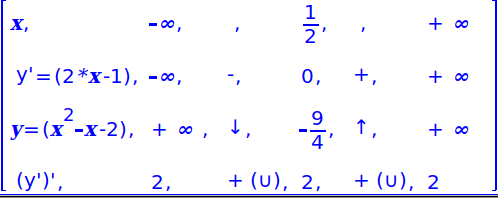
\includegraphics[width=0.75\textwidth]{xcas-tabvar1.png}
%\end{center}
% \begin{itemize}
%   \item The first row, the \texttt{x} row, gives the endpoint of
%   subintervals of the domain.  In this case, the subintervals go from
%   $-\infty$ to $1/2$ and from $1/2$ to $\infty$.
%   \item The second row, the \texttt{y'} row, gives the values of the
%   derivative at the values in the first row (or limits, in the case of
%   $\pm\infty$), and between them the sign ($+$ or $-$) of the
%   derivative in the corresponding subinterval.
%   \item The third row, the \texttt{y} row, gives the values of the
%   function at the values in the first row, and between them whether
%   the function is increasing or decreasing in the corresponding
%   subinterval.
%   \item The fourth row, the \texttt{y''}
%   row, gives the values of the second derivative at the values in the
%   first row, and between them whether the graph is concave up or
%   concave down in the subinterval.
% \end{itemize}
\item \textit{Input:}
\begin{center}
  \texttt{tabvar((2*t-1)/(t-1),t)}
\end{center}
\textit{Output:}
\begin{center}
\begin{tabular}{l}
\texttt{Function plot (2*t-1)/(t-1), variable t}\\
\texttt{Domain t<>1}\\
\texttt{Vertical asymptote x=1}\\
\texttt{Horizontal asymptote y=2}\\
\texttt{Horizontal asymptote y=2}\\
\texttt{Variations (2*t-1)/(t-1)}
\end{tabular}
\end{center}
\[
\left[
\begin{array}{ccccccc}
  t                                & -\infty &   &   1       &   1       &   & +\infty \\
  y'=-\frac1{\left(t-1\right)^{2}} &     0   & - & \text{||} & \text{||} & - & 0\\
  y=\frac{2 t-1}{t-1}              &    2    & \downarrow  &  -\infty
  &  +\infty  & \downarrow  & 2\\
  y''                              &    0    & - (\cap ) & || & || & +
  (\cup ) & 0
\end{array}
\right]
\]
\begin{center}
\begin{tabular}{l}
\texttt{plotfunc((2*t-1)/(t-1),t=((-0.1681472) .. 2.2222552))}\\
\texttt{Inside Xcas you can see the function with Cfg>Show>DispG.}
\end{tabular}
\end{center}
% \begin{center}
%   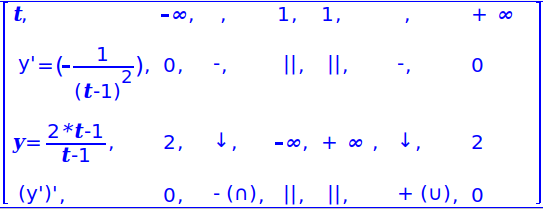
\includegraphics[width=0.75\textwidth]{xcas-tabvar2.png}
% \end{center}
Note that in this case, the value 1 appears twice in the first row, so
that both one-sided limits of \texttt{y} can be displayed at the
vertical asymptote $t=1$.  The values of 2 for \texttt{y} at $-\infty$
and $\infty$ indicate a horizontal asymptote of $y=2$.
\end{itemize}

\section{Limits: \texttt{limit}\label{sec:limit} \index{limit|textbf}}

The \texttt{limit} command computes limits, both at numbers and
infinities, and in the real case it can compute one-sided limits.
\begin{itemize}
  \item \texttt{limit} takes three mandatory and one optional argument.
  \begin{itemize}
    \item \textit{expr}, an expression.
    \item $x$, the name of a variable.
    \item $a$, the limit point.
    \item Optionally, \textit{side} (either 0, -1 or 1), to specify
    which side to take a one-sided limit (by default \textit{side}=0).
  \end{itemize}
  \item \texttt{limit(}\textit{expr,$x,a\,\langle,$side$\rangle$}\texttt{)}
  returns the limit of \textit{expr} as $x$ approaches $a$.
  \begin{itemize}
    \item If \textit{side} is 0 (the default), then the ordinary limit
    is returned.
    \item If \textit{side} is -1, then the limit from the left
    ($x<a$) is returned.
    \item If \textit{side} is 1, then the limit from the right
    ($x>a$) is returned.
  \end{itemize}
\end{itemize}
\textbf{Remark:}\\
It is also possible to put \texttt{x=a} as argument instead of
\texttt{x,a};
\texttt{limit(}\textit{expr,var}\texttt{=}\textit{pt[,side]}\texttt{)}
is equivalent to \texttt{limit(}\textit{expr,var,pt[,side]}\texttt{)}.

\smallskip

\noindent
\textbf{Examples.}
\begin{itemize}
\item \textit{Input:}
\begin{center}
  \texttt{limit(1/x,x,0,-1)}
\end{center}
\textit{or:}
\begin{center}
  \texttt{limit(1/x,x=0,-1)}
\end{center}
\textit{Output:}
\[
-\infty
\]
%\begin{center}\texttt{-(infinity)}\end{center}
\item \textit{Input:}
\begin{center}
  \texttt{limit(1/x,x,0,1)}
\end{center}
\textit{or:}
\begin{center}
  \texttt{limit(1/x,x=0,1)}
\end{center}
\textit{Output:}
\[
+\infty
\]
%\begin{center}\texttt{+(infinity)}\end{center}
\item \textit{Input:}
\begin{center}
  \texttt{limit(1/x,x,0,0)}
\end{center}
\textit{or:}
\begin{center}
  \texttt{limit(1/x,x,0)}
\end{center}
\textit{or:}
\begin{center}
  \texttt{limit(1/x,x=0)}
\end{center}
\textit{Output:}
\[
\infty
\]
(Note that $\infty$ or \textit{infinity} without an explicit
\texttt{+} or \textit{-} represents unsigned infinity.)
%\begin{center}\texttt{infinity}\end{center}
Hence, \texttt{abs(1/x)} approaches $+\infty$ when $x$ approaches $0$.
\end{itemize}

\smallskip

\noindent
\textbf{Exercises.}
\begin{itemize}
\item Find, for $n>2$, the limit as $x$ approaches $0$ of:
\[
 \frac{n\tan(x)-\tan(nx)}{\sin(nx)-n\sin(x)}
\]
\textit{Input:}
\begin{center}
  \texttt{limit((n*tan(x)-tan(n*x))/(sin(n*x)-n*sin(x)),x=0)}
\end{center}
\textit{Output:}
\[
2
\]
%\begin{center}\texttt{2}\end{center}
\item Find the limit as $x$ approaches $+\infty$ of
\[
\sqrt{x+\sqrt{x+\sqrt x}}-\sqrt x
\]
\textit{Input:}
\begin{center}
  \texttt{limit(sqrt(x+sqrt(x+sqrt(x)))-sqrt(x),x=+infinity)}
\end{center}
\textit{Output:}
\[
\frac{1}{2}
\]
%\begin{center}\texttt{1/2}\end{center}
\item Find the limit as $x$ approaches 0 of
\[
\frac{\sqrt{1+x+x^2/2}-\exp(x/2)}{(1-\cos(x))\sin(x)}
\]
\textit{Input:}
\begin{center}
  \texttt{limit((sqrt(1+x+x\^{}2/2)-exp(x/2))/((1-cos(x))*sin(x)),x,0)}
\end{center}
\textit{Output:}
\[
-\frac{1}{6}
\]
%\begin{center}\texttt{-1/6}\end{center}
\end{itemize}

% \smallskip

% \noindent
% \textbf{Remark.}\\
% To compute limits, it is sometimes better to quote the first argument.\\
% \textit{Input:}
% \begin{center}
%  \texttt{limit('(2*x-1)*exp(1/(x-1))',x=+infinity)}
% \end{center}
% Note that the first argument is quoted,  because it is better that
% this argument is not simplified (i.e. not evaluated).\\
% \textit{Output:}
% \begin{center}\texttt{+(infinity)}\end{center}

%\subsection{Integrals and limits}
%\index{limit}}

\section{Derivation and applications}

\subsection{Functional derivative: \texttt{function\_diff}
\index{function\_diff}}

The \texttt{function\_diff} command finds the derivatives of functions
(as opposed to expressions, see \secref{ssec:fnexpr}).
\begin{itemize}
  \item \texttt{function\_diff} takes one argument: $f$, a function.
  \item \texttt{function\_diff($f$)} returns the derivative $f'$ of $f$.
\end{itemize}

\smallskip

\noindent
\textbf{Examples.}
\begin{itemize}
\item \textit{Input:}
  \begin{center}
  \texttt{function\_diff(sin)}
  \end{center}
  \textit{Output:}
  \[
  \mathrm{x}\mapsto \cos \mathrm{x}
  \]
%\begin{center}\texttt{(` x`)->cos(` x`)}\end{center}
\item \textit{Input:}
  \begin{center}
  \texttt{function\_diff(sin)(x)}
  \end{center}
  \textit{Output:}
  \[
  \cos x
  \]
%\begin{center}\texttt{cos(x)}\end{center}
\item \textit{Input:}
  \begin{center}
  \begin{tabular}{l}
  \texttt{f(x):=x\^{}2+x*cos(x)}\\
  \texttt{function\_diff(f)}
  \end{tabular}
  \end{center}
  \textit{Output:}
  \[
  \mathrm{x}\mapsto \cos \mathrm{x}-\mathrm{x} \sin \mathrm{x}+2 \mathrm{x}
  \]
%\begin{center}\texttt{(` x`)->2*` x`+cos(` x`)+` x`*(-(sin(` x`)))}\end{center}
\item \textit{Input:}
  \begin{center}
  \texttt{function\_diff(f)(x)}
  \end{center}
  \textit{Output:}
  \[
  \cos x-x \sin x+2 x
  \]
\item   
%\begin{center}\texttt{cos(x)+x*(-(sin(x)))+2*x}\end{center}
To define the function $g$ as $f'$:\\
\textit{Input:}
\begin{center}
\texttt{g:=function\_diff(f)}
\end{center}
\item
The \texttt{function\_diff} instruction has the same effect as
using the expression derivative \texttt{diff} (see \secref{ssec:diff})
in conjunction with \texttt{unapply} (see \secref{ssec:unapply}):\\
\textit{Input:}
\begin{center}
\begin{tabular}{l}
\texttt{g:=unapply(diff(f(x),x),x)}\\
\texttt{g(x)}
\end{tabular}
\end{center}
\textit{Output:}
\[
\cos x-x \sin x+2 x
\]
%\begin{center}\texttt{cos(x)+x*(-(sin(x)))+2*x}\end{center}
\end{itemize}

\smallskip

\noindent
\textbf{Warning!!!}\\
In \texttt{Maple} mode (see \secref{ssec:lang}), for compatibility,
\texttt{D} may be used in place of \texttt{function\_diff}. For this
reason, it is impossible to assign a variable named \texttt{D} in
\texttt{Maple} mode (hence you can not name a geometric object \texttt{D}).

\subsection{Length of an arc: \texttt{arcLen}
\index{arcLen}
\label{sec:arclen}}

The \texttt{arcLen} command finds the lengths of curves in the plane,
which can either be given by an equation or a curve object.

To find the length of a curve given by an equation:
\begin{itemize}
  \item \texttt{arcLen} takes four arguments:
  \begin{itemize}
    \item \textit{expr}, an expression (resp. a list of two expressions $[$\textit{expr$_{1}$},\texttt{expr$_{2}$}$]$)
  involving a variable $x$.
  \item $x$, the name of the variable.
  \item $a$ and $b$, two values for the bounds of this variable.
  \end{itemize}
  \item \texttt{arcLen(}\textit{expr,}\texttt{$x,a,b$)}
  (resp.
  \texttt{arcLen([}\textit{expr$_{1}$},\textit{expr$_{2}$}\texttt{]}$x,a,b$\texttt{)})
  returns the length of the curve defined by 
  $y=f(x)=$\textit{expr} (resp. by
  $x_{1}=$\textit{expr$_{1}$},$x_{2}=$\textit{expr$_{2}$}) as $x$ varies from
  $a$ to $b$, using  the formula
  \[
    \mbox{arcLen}(f(x),x,a,b)= \int_{a}^{b}\sqrt{f'(x)^{2}+1}dx
  \]
  or
  \[
    \mbox{arcLen}(f(x),x,a,b)= \int_{a}^{b}\sqrt{x'(t)^{2}+y'(t)^{2}}dt
  \]
\end{itemize}

\smallskip

\noindent
\textbf{Examples.}
\begin{itemize}
\item Compute the length of the parabola $y=x^2$ from $x=0$ to $x=1$.\\
\textit{Input:}
\begin{center}
\texttt{arcLen(x\^{}2,x,0,1)}
\end{center}
\textit{or:}
\begin{center}
\texttt{arcLen([t,t\^{}2],t,0,1)}
\end{center}
\textit{Output:}
\[
\frac{2 \sqrt{5}-\ln \left(\sqrt{5}-2\right)}{4}
\]
%\begin{center}\texttt{-1/4*log(sqrt(5)-2)-(-(sqrt(5)))/2}\end{center}
\item Compute the length of the curve $y=\cosh(x)$ from $x=0$ to
$x=\ln(2)$.\\
\textit{Input:}
\begin{center}
\texttt{arcLen(cosh(x),x,0,log(2))}
\end{center}
\textit{Output:}
\[
\frac{3}{4}
\]
%\begin{center}\texttt{3/4}\end{center}
\item Compute the length of the circle $x=\cos(t),y=\sin(t)$ from $t=0$ to
$t=2*\pi$.\\
\textit{Input:}
\begin{center}
\texttt{arcLen([cos(t),sin(t)],t,0,2*pi)}
\end{center}
\textit{Output:}
\[
2 \pi
\]
%\begin{center}\texttt{2*pi}\end{center}
\end{itemize}

\smallskip

To find the length of a curve given by a curve object:
\begin{itemize}
  \item \texttt{arcLen} takes a single argument: \textit{curve}, a
  geometric curve defined in one of the graphics chapters (chapters
  \ref{chap:2dgraphics} and \ref{chap:3dgraphics}).
  \item \texttt{arcLen(}\textit{curve}\texttt{)} returns the length of the
  curve.
\end{itemize}

\smallskip

\noindent
\textbf{Examples.}
\begin{itemize}
\item \textit{Input:}
  \begin{center}
    \texttt{arcLen(circle(0,1,0,pi/2))}
  \end{center}
  \textit{Output:}
  \[
  \frac{1}{2} \pi
  \]
  %\begin{center}
  %  \tt
  % 1/2*pi
  %\end{center}
\item \textit{Input:}
  \begin{center}
    \texttt{arcLen(arc(0,1,pi/2))}
  \end{center}
  \textit{Output:}
  \[
  \frac{1}{4} \pi  \sqrt{2}
  \]
  % \begin{center}
  %   \tt
  %   sqrt(2)/4*pi
  % \end{center}
\end{itemize}

\subsection{Maximum and minimum of an expression: \texttt{fMax} \texttt{fMin}
\index{fMax}
\index{fMin}}

The \texttt{fMax} and \texttt{fMin} commands find where maxima and
minima occur.  They can do this for expressions of one variable or for
expressions of several variables subject to a set of constraints,
either equalities or inequalities.

The find the maximum and minimum of an expression with one variable:
\begin{itemize}
  \item \texttt{fMax} and \texttt{fMin} take two arguments:
  \begin{itemize}
    \item \textit{expr}, an expression involving one
    variable.
    \item Optionally, $x$, the name of the variable (by default 
    $x$=\texttt{x}).
  \end{itemize}
  \item \texttt{fMax(}\textit{expr}\texttt{$\,\langle,x\rangle$)} returns the
  value of $x$ that maximizes the expression.
  \item \texttt{fMin(}\textit{expr}\texttt{$\,\langle ,x\rangle$)} returns the
  value of $x$ that minimizes the expression.
\end{itemize}

\smallskip

\noindent
\textbf{Examples.}
\begin{itemize}
\item \textit{Input:}
  \begin{center}
  \texttt{fMax(sin(x),x)}
  \end{center}
  \textit{or:}
  \begin{center}
  \texttt{fMax(sin(x))}
  \end{center}
  \textit{or:}
  \begin{center}
  \texttt{fMax(sin(y),y)}
  \end{center}
  \textit{Output:}
  \[
  \frac{\pi}{2}
  \]
  %\begin{center}\texttt{pi/2}\end{center}
\item \textit{Input:}
  \begin{center}
  \texttt{fMin(sin(x),x)}
  \end{center}
  \textit{or:}
  \begin{center}
  \texttt{fMin(sin(x))}
  \end{center}
  \textit{or:}
  \begin{center}
  \texttt{fMin(sin(y),y)}
  \end{center}
  \textit{Output:}
  \[
  -\frac{\pi}{2}
  \]
\end{itemize}
%\begin{center}\texttt{-pi/2}\end{center}
% Input:
% \begin{center}
% \texttt{fMin(sin(x)\^{}2,x)}
% \end{center}
% Output:
% \[
% -\pi ,0,\pi ,-\frac{2}{2} \pi ,\frac{2}{2} \pi
% \]

% \begin{center}\texttt{0}\end{center}
\smallskip

The find the maximum and minimum of an expression with several
variables subject to constraints:
\begin{itemize}
  \item \texttt{fMax} and \texttt{fMin} take four mandatory and two
  optional arguments:
  \begin{itemize}
      \item \textit{expr}, an expression with several variables.
      \item \textit{constr}, a list of constraints (equalities and
        inequalities).
      \item \textit{vars}, a list of the variables.
      \item \textit{init}, an initial guess (which must be a list of
      nonzero reals representing a feasible point).
      \item Optionally, $\epsilon$, the precision.  If this isn't
      given, the default epsilon value is used (see \secref{ssec:confcomp},
      item \ref{enum:eps}).
      \item Optionally, $N$, the maximum number of iterations.
  \end{itemize}
  The expression \textit{expr} does not need to be differentiable.
  \item \texttt{fMax(}\textit{expr, constr ,vars ,init}\texttt{$\,\langle ,\epsilon\rangle \,\langle,N \rangle$)}
  returns the vector of values that maximizes \textit{expr} subject to
  the constraints \textit{constr}.
  \item \texttt{fMin(}\textit{expr, constr ,vars ,init}\texttt{$\,\langle ,\epsilon\rangle \,\langle,N \rangle$)}
  returns the vector of values that minimizes \textit{expr} subject to
  the constraints \textit{constr}.
\end{itemize}

\smallskip

\noindent
\textbf{Examples.}
\begin{itemize}
\item \textit{Input:}
  \begin{center}
    \texttt{fMax((x-2)\^{}2+(y-1)\^{}2,[-.25x\^{}2-y\^{}2+1>=0,x-2y+1=0],[x,y],[.5,.75])}
  \end{center}
  \textit{Output:}
  \[
  \left[-1.82287565553,-0.411437827766\right]
  \]
% \begin{center}
% 	\tt [-1.82287565553,-0.411437827766]
% \end{center}
\item \textit{Input:}
  \begin{center}
    	\texttt{fMin((x-5)\^{}2+y\^{}2-25,[y>=x\^{}2],[x,y],[1,1])}
  \end{center}
  \textit{Output:}
  \[
  \left[1.2347728625,1.52466402196\right]
  \]
  %\begin{center}
  %	\tt [1.2347728624961,1.5246640219568]
  %\end{center}
\end{itemize}

\smallskip

%Both \texttt{fMin} and \texttt{fMax} return the optimal solution as a
% vector. Note that the actual optimal value of the objective is not returned.

Although the initial point is required to be feasible, the algorithm
will sometimes succeed even with a poor choice of initial point.
%if it is infeasible.
Note that the initial value of a variable must not be zero.

% \subsection{Table of values and graph: \texttt{tablefunc} and \texttt{plotfunc}
% \index{tablefunc|textbf}
% \index{plotfunc}}

% The \texttt{tablefunc} command is used inside a spreadsheet
% (opened with \texttt{Alt+t}, see \secref{sec:spreadsheet})
% and it returns a template to fill two columns with the table of values
% of a function.

% \texttt{tablefunc} is a command that should be used inside a
% spreadsheet (opened with \texttt{Alt+t}), it returns a template to
% fill two columns, with the table of values of a function. If the step
% value is 1, \texttt{tablefunc(ex,n,n0,1)}, where \texttt{ex} is an
% expression depending on \texttt{n}, will fill the spreadsheet with the
% values of the sequence $u_n=ex$ for $n=n0,\ n0+1,\ n0+2,\ldots$.

% \textbf{Example}: display the values of the sequence $u_n=\sin(n)$\\
% Select a cell of a spreadsheet (for example \texttt{C0}) and input in
% the command line:
% \begin{center}
%   \texttt{tablefunc(sin(n),n,0,1)}
% \end{center}
% Output:
% \begin{center}
%   \texttt{two columns: n and sin(n)}
% \end{center}
% \begin{itemize}
% \item in the column C: the variable name \texttt{n}, the value of the step
% (this value should be equal to 1 for a sequence),
% the value of \texttt{n0} (here 0), then a recurrence
% formula (\texttt{C2+C\$1}, \ldots).
% \item  in the column D: \texttt{sin(n)}, \texttt{"Tablefunc"}, then a
% recurrence formula.
% \item For each row,
% the values of the sequence $\texttt{u_n=\sin(n)}$ correspond to
% the values of \texttt{n} starting from \texttt{n=n0} (here 0).
% \end{itemize}


% \texttt{tablefunc} is a special command that should be run from inside
% the spreadsheet. It returns the evaluation of an expression $ex$
% depending on a variable $x$ for $x=x_0,\ x_0+h,\ldots$:
% \begin{center}
% \texttt{tablefunc(ex,x,x\_0,h)} or \texttt{tablefunc(ex,x)}
% \end{center}
% In the latter case, the default value for $\texttt{x_0}$
% is the default minimum value of $x$ from the graphic configuration
% and the default value for the step $h$ is 0.1 times the difference
% between the default maximum and minimum values of $x$ (from the
% graphic configuration).\\
% Example: type \texttt{Alt+t} to open a spreadsheet if none are open.
% Then select a cell of the spreadsheet (for example \texttt{C0}) and to get
% the table of \texttt{"sinus"}, input in the command line of the spreadsheet:
% \begin{center}\texttt{tablefunc(sin(x),x)}\end{center}
% This will fill two columns with the numeric value of \texttt{x} and
% \texttt{sin(x)}:
% \begin{itemize}
% \item in the first column the variable \texttt{x},
% the value of the step \texttt{h}
% (1.0),  the minimum value of $x$ (-5.0), then a formula, for example
% {\tt=C2+C\$1}, and the remaining rows
% of the column is filled by pasting this formula.
% \item in the next column the function \texttt{sin(x)}, the word
% "Tablefunc", a formula,
% for example \texttt{=evalf(subst(D\$0,C\$0,C2))}, and the remaining rows
% of the column are filled by pasting this formula.
% \end{itemize}
% Hence the values of \texttt{sin(x)} are on the same rows as the values
% of \texttt{x}. Note that the step and begin value and the expression
% may be easily changed by modifying the correspondent cell.

% The graphic representation may be plotted with the \texttt{plotfunc}
% command (see \ref{ssec:plotfunc}).

\subsection{Derivatives and partial derivatives
\index{diff|textbf}
\index{derive|textbf}
\index{deriver|textbf}
\label{ssec:diff}}

The \texttt{diff} command computes derivatives
and partial derivatives of expressions.\\
\texttt{derive} is a synonym for \texttt{diff}.

\smallskip

To compute first order derivatives:
\begin{itemize}
  \item \texttt{diff} takes one mandatory
  argument and one optional argument:
  \begin{itemize}
    \item \textit{expr}, an expression or a list of expressions.
    \item Optionally, $x$, a variable (resp. a list of
      variable names, see several variable functions in
      \ref{sec:plusvar}).  If the only variable is \texttt{x}, this
      second argument can be omitted.
  \end{itemize}
  \item \texttt{diff(}\textit{expr}$\,\langle ,x \rangle$\texttt{)}
  returns the derivative (resp. a vector of derivatives) of the
  expression \textit{expr} (or list of expressions) with respect to the
  variable $x$ (resp. with respect to each variable in the list
  $x$).
\end{itemize}

\smallskip

\noindent
\textbf{Examples.}
\begin{itemize}
\item Compute:
\[\frac {\partial (x y^2 z^3+x y z)}{\partial z}\]
\textit{Input:}
\begin{center}
\texttt{diff(x*y\^{}2*z\^{}3+x*y*z,z)}
\end{center}
\textit{Output:}
\[
3 x y^{2} z^{2}+x y
\]
%\begin{center}\texttt{x*y\^{}2*3*z\^{}2+x*y}\end{center}
\item Compute the 3 first order partial derivatives of $x*y^2*z^3+x*y*z$.\\
\textit{Input:}
\begin{center}
\texttt{diff(x*y\^{}2*z\^{}3+x*y,[x,y,z])}
\end{center}
\textit{Output:}
\[
\left[y^{2} z^{3}+y,2 x y z^{3}+x,3 x y^{2} z^{2}\right]
\]
%\begin{center}\texttt{[y\^{}2*z\^{}3+y*z, x*2*y*z\^{}3+x*z, x*y\^{}2*3*z\^{}2+x*y]}\end{center}
\item
Compute:
\[\frac {\partial^3 (x.y^2.z^3+x.y.z)}{\partial y\partial^2 z}\]
\textit{Input:}
\begin{center}
\texttt{diff(x*y \^{}2*z\^{}3+x*y*z,y,z\$2)}
\end{center}
\textit{Output:}
\[
12 x y z
\]
% \begin{center}\texttt{x*2*y*3*2*z}\end{center}
\end{itemize}

\smallskip

To compute higher order derivatives:
\begin{itemize}
  \item \texttt{diff} takes more than two arguments:
  \begin{itemize}
    \item \textit{expr}, an expression.
    \item $x_{1},x_{2}$\textit{\ldots}, the names of the
    derivation variables.  Note that for repeated variables, you can
    use the \texttt{\$} operator (see \secref{ssec:makeseq}) followed by
  the number of derivations with respect to the variable; for
  example, instead of writing $x,x,x$ you could write $x\$3$.
  \end{itemize}
  \item \texttt{diff(}\textit{expr},$x_{1},x_{2}$,\dots\texttt{)} returns the
  partial derivative of \textit{expr} with respect to the variables
  $x_{1},x_{2},$\textit{\ldots}.
\end{itemize}

\smallskip

\noindent
\textbf{Examples.}
\begin{itemize}
\item Compute:
\[\frac {\partial^2 (x y^2 z^3+x y z)}{\partial x\partial z}\]
\textit{Input:}
\begin{center}
\texttt{diff(x*y\^{}2*z\^{}3+x*y*z,x,z)}
\end{center}
\textit{Output:}
\[
3 y^{2} z^{2}+y
\]
%\begin{center}\texttt{y\^{}2*3*z\^{}2+y}\end{center}
\item Compute:
\[\frac {\partial^3 (x y^2 z^3+x y z)}{\partial x\partial^2 z}\]
\textit{Input:}
\begin{center}
\texttt{diff(x*y\^{}2*z\^{}3+x*y*z,x,z,z)}
\end{center}
\textit{or:}
\begin{center}
\texttt{diff(x*y\^{}2*z\^{}3+x*y*z,x,z\$2)}
\end{center}
\textit{Output:}
\[
6 y^{2} z
\]
%\begin{center}\texttt{y\^{}2*3*2*z}\end{center}
\item Compute the third derivative of:
\[\frac{1}{x^2+2}\]
\textit{Input:}
\begin{center}
\texttt{normal(diff((1)/(x\^{}2+2),x,x,x))}
\end{center}
\textit{or:}
\begin{center}
\texttt{normal(diff((1)/(x\^{}2+2),x\$3))}
\end{center}
\textit{Output:}
\[
\frac{-24 x^{3}+48 x}{x^{8}+8 x^{6}+24 x^{4}+32 x^{2}+16}
\]
%\begin{center}\texttt{(-24*x\^{}3+48*x)/(x\^{}8+8*x\^{}6+24*x\^{}4+32*x\^{}2+16)}\end{center}
\end{itemize}

\smallskip

\noindent
\textbf{Remark.}
\begin{itemize}
\item
Note the difference between \texttt{diff($f,x,y$)} and
\texttt{diff($f$,[$x,y$])}:\\
\texttt{diff($f,x,y$)} returns $\displaystyle
\frac{\partial^2(f)}{\partial x\partial y}$ and
\texttt{diff($f,[x,y]$)} returns
$\displaystyle[\frac{\partial(f)}{\partial x},
\frac{\partial (f)}{\partial y}]$
\item Never define a derivative function with
\texttt{f1(x):=diff(f(x),x)}.
Indeed, \texttt{x} would mean two different things Xcas is unable to
deal with: on the left hand side, \texttt{x} is the variable name to
define the $f_1$ function, and on the right hand side, \texttt{x} is
the differentiation variable. The right way to define a derivative is
either with \texttt{function\_diff} or:
\begin{center}
\texttt{f1:=unapply(diff(f(x),x),x)}
\end{center}
\end{itemize}


\subsection{Implicit differentiation: \texttt{implicitdiff}
\index{implicitdiff}}

The \texttt{implicitdiff} command can differentiate implicitly defined
functions or expressions containing implicitly defined functions.  It
has three different calling sequences.

\medskip

\noindent
To implicitly differentiate dependent variables:
\begin{itemize}
  \item \texttt{implicitdiff} takes four arguments:
  \begin{itemize}
    \item \textit{constraints}, an equation or list of equations which
    implicitly define the dependent variables as functions of the
    independent variables; these will be of the form
    \[g_i(x_{1},\ldots,x_{n},y_{1},\ldots,y_{m})=0\]
    for
    $i=1,2,\ldots,m$, where $x_{1},ldots,x_{n}$ are the
    independent variables and $y_{1},\ldots,y_{m}$ are the
    dependent variables.
    \item \textit{depvars}, the list of dependent variables, where each
    dependent variable can optionally be written as a function of the
    $x_{i}$ or the name written as a function of the
    independent variables $y_{i}(x_{1},\ldots,x_{n})$.  If there is only
    one dependent variable, this can be omitted.
    \item $y$, a dependent variable or a list of dependent variables to
    be differentiated.
    \item \textit{diffvars}, a sequence of independent variables
    $x_{i_{1}},\ldots,x_{i_k}$ with respect to differentiate.
  \end{itemize}
  \item \texttt{implicitdiff(}\textit{constraints $\,\langle$,depvars
  $\rangle$],y,diffvars}\texttt{)}
  returns the derivative (or list of derivatives) of $y$ with respect to
  \textit{diffvars}.
\end{itemize}

\smallskip

\noindent
\textbf{Examples.}
\begin{itemize}
\item \textit{Input:}
\begin{center}
\texttt{implicitdiff(x\^{}2*y+y\^{}2=1,y,x)}
\end{center}
\textit{Output:}
\[
-\frac{2 x y}{x^{2}+2 y}
\]
%\begin{center}
%\texttt{-2*x*y/(x\^{}2+2*y)}
%\end{center}
\item \textit{Input:}
\begin{center}
\texttt{implicitdiff([x\^{}2+y=z,x+y*z=1],[y(x),z(x)],y,x)}
\end{center}
\textit{Output:}
\[
\frac{-2 x y-1}{y+z}
\]
%\begin{center}
%\texttt{(-2*x*y-1)/(y+z)}
%\end{center}
\end{itemize}

\smallskip

To find a specified derivative of an expression containing
implicitly defined functions:
\begin{itemize}
  \item  \texttt{implicitdiff} takes four arguments:
  \begin{itemize}
    \item \textit{expr}, a differentiable expression involving
    independent variables $x_{1},x_{2},\ldots,x_{n}$
    and dependent variables $y_{1},y_{2},\ldots,y_{m}$.
    \item \textit{constraints}, an equation or list of equations which
    implicitly define the dependent variables as functions of the
    independent variables; these will be of the form
    \[g_i(x_{1},\ldots,x_{n},y_{1},\ldots,y_{m})=0\]
    for
    $i=1,2,\ldots,m$.
    \item \textit{depvars}, the dependent variable or list of dependent
    variables,  where each dependent variable can either be the
    variable name $y_{i}$ or the name written as a function of
    the independent variables $y_{i}(x_{1},\dots,x_{n})$).
    \item \textit{diffvars}, a sequence of independent variables
    $x_{i_{1}},\ldots,x_{i_k}$ with respect to which \textit{expr} is differentiated.
  \end{itemize}
  \item \texttt{implicitdiff(}\textit{expr,implicitdef,depvars,diffvars}\texttt{)}
  returns the expression \textit{expr} differentiated with respect to
  \textit{diffvars}.
\end{itemize}

\smallskip

\noindent
\textbf{Example.}\\
\textit{Input:}
\begin{center}
\texttt{implicitdiff(x*y,-2x\^{}3+15x\^{}2*y+11y\^{}3-24y=0,y(x),x)}
\end{center}
\textit{Output:}
\[
\frac{2 x^{3}-5 x^{2} y+11 y^{3}-8 y}{5 x^{2}+11 y^{2}-8}
\]
%\begin{center}
%\texttt{(2*x\^{}3-5*x\^{}2*y+11*y\^{}3-8*y)/(5*x\^{}2+11*y\^{}2-8)}
%\end{center}

\smallskip

\noindent
To find all $k$th order derivatives of an expression
involving implicitly defined functions:
\begin{itemize}
  \item \texttt{implicitdiff} takes four mandatory arguments and one
  optional argument:
\begin{itemize}
  \item \textit{expr}, a differentiable expression involving
    independent variables  $x_{1},x_{2},\ldots,x_{n}$
    and dependent variables $y_{1},y_{2},\ldots,y_{m}$.
  \item \textit{constraints}, an equation or list of equations which
     implicitly define the dependent variables as functions of the
     independent variables; these will be of the form
     \[g_i(x_{1},\ldots,x_{n},y_{1},\ldots,y_{m})=0\] for
     $i=1,2,\ldots,m$.
  \item \texttt{vars}, a list $[x_{1},\ldots,x_{n},y_{1},\ldots, y_{m}]$
     of the independent and dependent variables
     entered as symbols in single list such that dependent variables
     come last.
  \item \texttt{order=$k$}, where $k$ is the order of the derivatives
  to be taken.
  \item Optionally, $a$, a point where the partial derivatives
  should be evaluated at.
  \end{itemize}
  \item
  \texttt{implicitdiff(}\textit{expr,implicitdef,vars,}\texttt{order=}$k
  \,\langle,a\rangle$\texttt{)}
  returns all partial derivatives of order $k$.  If $k=1$ they are
  returned in a single list, which represents the gradient of
  \texttt{expr} with respect to independent variables. If $k=2$ the
  corresponding Hessian matrix is returned (see \secref{ssec:hessian}). 
  If $k>2$, a table with
  keys in form \texttt{[$k_{1}$,$k_{2}$,..,$k_{n}$]}, where
  $\sum_{i=1}^{n}k_i=k$, is returned. Such a key corresponds to
  \[\frac{\partial^k f}{\partial \textit{var}_1^{k_1}\,\partial
  \textit{var}_2^{k_2}\,\cdots\,\partial \textit{var}_n^{k_n}}. \]
\end{itemize}

\smallskip

\noindent
\textbf{Examples.}
\begin{itemize}
\item \textit{Input:}
  \begin{center}
  \begin{tabular}{l}
  \texttt{f:=x*y*z; g:=-2x\^{}3+15x\^{}2*y+11y\^{}3-24y=0;}\\
  \texttt{implicitdiff(f,g,[x,z,y],order=1)}
  \end{tabular}
  \end{center}
  \textit{Output:}
  \[
  \left[\frac{2 x^{3} z-5 x^{2} y z+11 y^{3} z-8 y z}{5 x^{2}+11 y^{2}-8},x y\right]
  \]
%\begin{center}
%\texttt{[(2*x\^{}3*z-5*x\^{}2*y*z+11*y\^{}3*z-8*y*z)/(5*x\^{}2+11*y\^{}2-8),}\\
%\texttt{x*y]}
%\end{center}
\item \textit{Input:}
  \begin{center}
  \texttt{implicitdiff(f,g,[x,z,y],order=2,[1,-1,0])}
  \end{center}
  \textit{Output:}
  \[
  \left[
     \begin{array}{cc}
         \frac{64}{9}&-\frac{2}{3}\\
         -\frac{2}{3}&0
     \end{array}
  \right]
  \]
%\begin{center}
%\texttt{[[64/9,-2/3],[-2/3,0]]}
%\end{center}
\item In the next example, the value of $\frac{\partial^4 f}{\partial x^4}$
is computed at the point $(x=0,y=0,z)$.\\
\textit{Input:}
\begin{center}
\begin{tabular}{l}
\texttt{pd:=implicitdiff(f,g,[x,z,y],order=4,[0,z,0]);}\\
\texttt{pd[4,0]}
\end{tabular}
\end{center}
\textit{Output:}
\[
-2 z
\]
%\begin{center}
%\texttt{-2*z}
%\end{center}
\end{itemize}

% \subsection{Implicit differentiation: \texttt{implicitdiff}}

% \texttt{implicitdiff} is called with one of the following three sets
% of parameters:
% \begin{enumerate}
% \item \texttt{expr}, \texttt{constr}, \texttt{depvars}, \texttt{diffvars}
% \item \texttt{constr}, \texttt{[depvars]}, \texttt{y}, \texttt{diffvars}
% \item \texttt{expr}, \texttt{constr}, \texttt{vars}, \texttt{order=k}, \texttt{[pt]}
% \end{enumerate}
% Details on parameters:
% \begin{itemize}
% \item \texttt{expr}: differentiable expression $ f(x_1,x_2,\dots,x_n,y_1,y_2,\dots,y_m) $
% \item \texttt{constr}: (list of) equality constraint(s) $ g_i(x_1,\dots,x_n,y_1,\dots,y_m)=0 $ or vanishing expression(s) $ g_i $, where $ i=1,2,\dots,m $
% \item \texttt{depvars}: (list of) dependent variable(s) $ y_1,y_2,\dots,y_m $, each of which may be entered as a symbol, e.g.~\texttt{yi}, or a function of independent variable(s), e.g.~\texttt{yi(x1,x2,..,xn)}
% \item \texttt{diffvars}: sequence of variables $ x_{i_1},x_{i_2},\dots,x_{i_k} $ with respect to which is \texttt{expr} differentiated
% \item \texttt{vars}: independent and dependent variables entered as symbols in single list such that dependent variables come last, e.g.~\texttt{[x1,..,xn,y1,..,ym]}
% \item \texttt{y}: (list of) dependent variable(s) $ y_{j_1},y_{j_2},\dots,y_{j_l} $ that need to be differentiated
% \end{itemize}
% Dependent variables $ y_1,y_2,\dots,y_m $ are implicitly defined with $ m $ constraints in \texttt{constr}. By implicit function theorem, the Jacobian matrix of $ \mathbf{g}=(g_1,g_2,\dots,g_m) $ has to be full rank.

% When calling \texttt{implicitdiff}, first two sets of parameters are
% used when specific partial derivative is needed. In the first case,
% \texttt{expr} is differentiated with respect to \texttt{diffvars}.

% \noindent
% Input:
% \begin{center}
%\texttt{implicitdiff(x*y,-2x\^{}3+15x\^{}2*y+11y\^{}3-24y=0,y(x),x)}
% \end{center}
% Output:
% \begin{center}
% \texttt{(2*x\^{}3-5*x\^{}2*y+11*y\^{}3-8*y)/(5*x\^{}2+11*y\^{}2-8)}
%\frac{2 x^{3}-5 x^{2} y+11 y^{3}-8 y}{5 x^{2}+11 y^{2}-8}
% \end{center}
% In the second case (elements of) \texttt{y} is differentiated. If \texttt{y} is a list of symbols, a list containing their derivatives will be returned. The following examples compute $ \frac{\mathrm{d}\,y}{\mathrm{d}\,x} $.\\
% Input:
% \begin{center}
% \texttt{implicitdiff(x\^{}2*y+y\^{}2=1,y,x)}
% \end{center}
% Output:
% \begin{center}
% \texttt{-2*x*y/(x\^{}2+2*y)}
% \end{center}
% Input:
% \begin{center}
% \texttt{implicitdiff([x\^{}2+y=z,x+y*z=1],[y(x),z(x)],y,x)}
% \end{center}
% Output:
% \begin{center}
% \texttt{(-2*x*y-1)/(y+z)}
% \end{center}
% In the next example, $ \frac{\mathrm{d}\,y}{\mathrm{d}\,x} $ and $ \frac{\mathrm{d}\,z}{\mathrm{d}\,x} $ are computed.\\
% Input:
% \begin{center}
% \texttt{implicitdiff([-2x*z+y\^{}2=1,x\^{}2-exp(x*z)=y],}\\
% \texttt{[y(x),z(x)],[y,z],x)}
% \end{center}
% Output:
% \begin{center}
% \texttt{[2*x/(y*exp(x*z)+1),}\\
% \texttt{(2*x*y-y*z*exp(x*z)-z)/(x*y*exp(x*z)+x)]}
% \end{center}

% For the third case of input syntax, all partial derivatives of order
% equal to \texttt{order}, i.e.~$ k $, are computed. If $ k=1 $ they are
% returned in a single list, which represents the gradient of
% \texttt{expr} with respect to independent variables. For $ k=2 $ the
% corresponding hessian matrix is returned. When $ k>2 $, a table with
% keys in form \texttt{[k1,k2,..,kn]}, where $ \sum_{i=1}^nk_i=k $, is
% returned. Such key corresponds to \[ \frac{\partial^k f}{\partial
% x_1^{k_1}\,\partial x_2^{k_2}\,\cdots\,\partial x_n^{k_n}}. \] Input:
% \begin{center}
% \texttt{f:=x*y*z; g:=-2x\^{}3+15x\^{}2*y+11y\^{}3-24y=0;}\\
% \texttt{implicitdiff(f,g,[x,z,y],order=1)}
% \end{center}
% Output:
% \begin{center}
% \texttt{[(2*x\^{}3*z-5*x\^{}2*y*z+11*y\^{}3*z-8*y*z)/(5*x\^{}2+11*y\^{}2-8),}\\
% \texttt{x*y]}
% \end{center}
% Input:
% \begin{center}
% \texttt{implicitdiff(f,g,order=2,[1,-1,0])}
% \end{center}
% Output:
% \begin{center}
% \texttt{[[64/9,-2/3],[-2/3,0]]}
% \end{center}
% In the next example, the value of $ \frac{\partial^4 f}{\partial x^4} $ is computed at point $ (x=0,y=0,z) $.\\
% Input:
% \begin{center}
% \texttt{pd:=implicitdiff(f,g,[x,z,y],order=4,[0,z,0]);}\\
% \texttt{pd[4,0]}
% \end{center}
% Output:
% \begin{center}
% \texttt{-2*z}
% \end{center}

\subsection{Numerical differentiation: \texttt{numdiff}\index{numdiff}}

The \texttt{numdiff} command finds numerical approximations to
derivatives.
\begin{itemize}
  \item \texttt{numdiff} takes three mandatory arguments and one
  optional argument.
  \begin{itemize}
    \item $X=[\alpha_0,\alpha_1,\dots,\alpha_n]$,
    $Y=[\beta_0,\beta_1,\dots,\beta_n]$, two lists of real numbers,
    where $n\geq 1$.
    \item $x_0$, a real number.
    \item Optionally, $m$, an integer or a sequence of integers (by default 1).
  \end{itemize}
  \item \texttt{numdiff($X,Y,x_0\,\langle,m\rangle$)}
  returns an approximation of the $m$-th derivative of a function $f$
  at $x_0$, or a sequence of derivatives of order given by the
  sequence $m$,  where $f$ has values given by $f(\alpha_k)=\beta_k$,
  $k=0,1,\dots,n$.
\end{itemize}
\texttt{numdiff} uses Fornberg's algorithm described in ``Generation
of Finite Difference Formulas on Arbitrarily Spaced Grids'', {\it
Mathematics of Computation}, 51(184):699--706, 1988. The complexity of
this algorithm is $O(n^2m)$ in both time and space. To avoid numerical
instabilities, {\tt numdiff} operates in exact arithmetic.

Note that $\alpha_0,\alpha_1,\dots,\alpha_n$ do not have to be equally
spaced, but they must be mutually different and input in ascending
order. There are no restrictions on the choice of $x_0$.

\smallskip

\noindent
\textbf{Examples.}
\begin{itemize}
\item 
Let $f(x)=\sin(x)\mathrm{e}^{-x}$, $x\in[0,1]$. Sample this function
at the points in
\[ 
X=[0,0.1,0.2,0.4,0.5,0.7,0.8,1] 
\]
to approximate $f''(1/\pi)$.\\
\textit{Input:}
\begin{center}
\begin{tabular}{l}
\texttt{f:=unapply(sin(x)*exp(-x),x):;}\\
\texttt{X:=[0,0.1,0.2,0.4,0.5,0.7,0.8,1]:;}\\
\texttt{Y:=apply(f,X):;}
\end{tabular}
\end{center}
Now you can approximate the second derivative of $f$ at the point
$x_0=\frac{1}{\pi}$.\\
\textit{Input:}
\begin{center}
\begin{tabular}{l}
\texttt{x0:=1/pi:;}\\
\texttt{d:=numdiff(X,Y,x0,2)}
\end{tabular}
\end{center}
\textit{Output:}
\[
-1.38167652799
\]
Finally, compute the relative error of the obtained approximation.\\
\textit{Input:}
\begin{center}
  \texttt{abs(d-f''(x0))/abs(f''(x0))*100}
\end{center}
\textit{Output:}
\[
2.82975186496\times10^{-5}
\]
The result is expressed in percentages.
\item
Use a sequence of values for the parameter $m$ to find a list of
approximations of the respective derivatives at $x_0$. This is faster
than calling \texttt{numdiff} to approximate one derivative at a time.\\
Specifically, approximate the zeroth, first and second derivative of
the function
\[ 
f(x)=1-\frac{1}{1+x^2},\quad x\in[0,1], 
\]
at the point $x_0=\gamma$, where $\gamma\approx 0.57722$ is the
Euler-Mascheroni constant, by sampling $f$ at 21 equidistant points in
the segment $[0,1]$.\\
\textit{Input:}
\begin{center}
\begin{tabular}{l}
  \texttt{f:=unapply(1-1/(1+x\^{}2),x)}\\
  \texttt{X:=[(0.05*k)\$(k=0..20)]:; Y:=apply(f,X):;}\\
  \texttt{numdiff(X,Y,euler\_gamma,0,1,2)}
\end{tabular}
\end{center}
\textit{Output:}
\[
\left[0.249912571952,0.649519026356,0.000393517941567\right]
\]
The correct values are $f(\gamma)=0.249912571952$,
$f'(\gamma)=0.649519026356$ and $f''(\gamma)=0.000393517946748$.
\end{itemize}

\smallskip

\texttt{numdiff} can be used for generating custom finite-difference
stencils for approximation of derivatives.

\smallskip

\noindent
\textbf{Example.}\\
Let $X=[-1,0,2,4]$, $Y=[a,b,c,d]$ and $x_0=1$. To obtain an
approximation formula for the second derivative:\\
\textit{Input:}
\begin{center}
  \texttt{numdiff([-1,0,2,4],[a,b,c,d],1,2)}
\end{center}
\textit{Output:}
\[
\frac{2}{5} a-\frac{b}{2}+\frac{d}{10}
\]
The approximation is always a linear combination of elements in $Y$,
regardless of $X$, $x_0$ and $m$. 

\smallskip

Given the lists
$X=[\alpha_0,\alpha_1,\dots,\alpha_n]$ and $Y=[\beta_0,\beta_1,\dots,\beta_n]$,
the Lagrange polynomial passing through points
$(\alpha_k,\beta_k)$ where $k=0,1,\dots,n$ can be obtained by setting
$m=0$ and entering a symbol for $x_0$.

\smallskip

\noindent
\textbf{Example.}\\
Let $X=[-2,0,1]$ and $Y=[2,4,1]$:\\
\textit{Input:}
\begin{center}
  \texttt{expand(numdiff([-2,0,1],[2,4,1],x,0))}
\end{center}
\textit{Output:}
\[
-\frac{4}{3} x^{2}-\frac{5}{3} x+4
\]
The same result is obtained by entering \texttt{lagrange([-2,0,1],[2,4,1],x)}.

\section{Integration}

\subsection{Antiderivative and definite integral: \texttt{integrate} \texttt{int} \texttt{Int}
\index{integrate}
\index{Int}
\index{int}
\label{ssec:integrate}}

The \texttt{int} and \texttt{integrate} commands compute a primitive
or a definite integral. A difference between the two commands is that if
you input \texttt{quest()} just after the evaluation of
\texttt{integrate}, the answer is written with the $\int$ symbol.

\texttt{Int} is the inert form of \textit{integrate}; namely, it
evaluates to \textit{integrate} for later evaluation.

\smallskip

\noindent
To find a primitive (an antiderivative):
\begin{itemize}
  \item \texttt{int} (or \texttt{integrate}) takes one mandatory
  argument and one optional argument:
  \begin{itemize}
    \item \textit{expr}, an expression.
    \item Optionally, $x$, the name of a
    variable (by default the value is \texttt{x}, so if the variable is
    \texttt{x} the second argument is unnecessary).
  \end{itemize}
  \item \texttt{int(}\textit{expr}\texttt{$\,\langle,x\rangle$)}
  (or \texttt{integrate(}\textit{expr}\texttt{$\,\langle,x\rangle$)}) returns a
  primitive of \textit{expr} with respect to $x$.
\end{itemize}

\smallskip

\noindent
\textbf{Examples.}
\begin{itemize}
\item \textit{Input:}
  \begin{center}
  \texttt{integrate(x\^{}2)}
  \end{center}
  \textit{Output:}
  \[
  \frac{x^{3}}{3}
  \]
  %\begin{center}\texttt{x\^{}3/3}\end{center}
\item \textit{Input:}
  \begin{center}
  \texttt{integrate(t\^{}2,t)}
  \end{center}
  \textit{Output:}
  \[
  \frac{t^{3}}{3}
  \]
  %\begin{center}\texttt{t\^{}3/3}\end{center}
\end{itemize}

\smallskip

To evaluate a definite integral:
\begin{itemize}
  \item \texttt{int} (or \texttt{integrate})
    takes four arguments:
  \begin{itemize}
    \item \textit{expr}, an expression.
    \item $x$, the variable.
    \item $a$ and $b$, the bounds of the definite integral.
  \end{itemize}
  \item \texttt{int(}\textit{expr,$x,a,b$}\texttt{)}
  (or \texttt{integrate(}\textit{expr,$x,a,b$}\texttt{)}) returns
  the exact value of the definite integral if the computation was
  successful or an unevaluated integral otherwise.
\end{itemize}

\smallskip

\noindent
\textbf{Examples.}
\begin{itemize}
\item \textit{Input:}
  \begin{center}
  \texttt{integrate(x\^{}2,x,1,2)}
  \end{center}
  \textit{Output:}
  \[
  \frac{7}{3}
  \]
%\begin{center}\texttt{7/3}\end{center}
\item \textit{Input:}
  \begin{center}
  \texttt{integrate(1/(sin(x)+2),x,0,2*pi)}
  \end{center}
  \textit{Output:}
  \[
  \frac{2}{3} \pi  \sqrt{3}
  \]
\end{itemize}

\smallskip

\texttt{Int} is the inert form of \texttt{integrate}, it prevents
evaluation, for example to avoid a symbolic computation that might not
be successful if you just want a numeric evaluation.

\smallskip

\noindent
\textbf{Example.}\\
\textit{Input:}
\begin{center}
\texttt{evalf(Int(exp(x\^{}2),x,0,1))}
\end{center}
\textit{or:}
\begin{center}
\texttt{evalf(int(exp(x\^{}2),x,0,1))}
\end{center}
\textit{Output:}
\[
1.46265174591
\]
%\end{itemize}
%\begin{center}\texttt{1.46265174591}\end{center}

\smallskip

\noindent
\textbf{Exercises.}
\begin{enumerate}
  \item 
Let
\[
f(x)=\frac{x}{x^2-1}+\ln(\frac{x+1}{x-1})
\]
Find a primitive of $f$.\\
\textit{Input:}
\begin{center}
\texttt{int(x/(x\^{}2-1)+ln((x+1)/(x-1)))}
\end{center}
\textit{Output:}
\[
x \ln \left(\frac{x+1}{x-1}\right)+\frac{2}{2} \ln \left|x^{2}-1\right|+\frac{\ln \left|x^{2}-1\right|}{2}
\]
%\begin{center}\texttt{x*log((x+1)/(x-1))+log(x\^{}2-1)+1/2*log(2*x\^{}2/2-1)}\end{center}
Alternatively, define the function \texttt{f},\\
\textit{Input:}
\begin{center}
\texttt{f(x):=x/(x\^{}2-1)+ln((x+1)/(x-1))}
\end{center}
\textit{then:}
\begin{center}
\texttt{int(f(x))}
\end{center}
The output, of course, will be the same.

\smallskip

\noindent
\textbf{Warning.}\\
For \texttt{Xcas}, \texttt{log} is the natural logarithm (like
\texttt{ln}); \texttt{log10} is the base-10 logarithm.

\item 
Compute:
\[
\int \frac {2}{x^6+2 \cdot x^4+x^2} \ dx
\]
\textit{Input:}
\begin{center}
\texttt{int(2/(x\^{}6+2*x\^{}4+x\^{}2))}
\end{center}
\textit{Output:}
\[
2 \left(\frac{-3 x^{2}-2}{2 \left(x^{3}+x\right)}-\frac{3}{2} \arctan x\right)
\]
%\begin{center}\texttt{2*((3*x\^{}2+2)/(-(2*(x\^{}3+x)))+-3/2*atan(x))}\end{center}

\item
Compute:
\[
\int \frac{1}{\sin(x)+\sin(2 \cdot x )} \ dx
\]
\textit{Input:}
\begin{center}
\texttt{integrate(1/(sin(x)+sin(2*x )))}
\end{center}
\textit{Output:}
\[
2 \left(\frac{\ln \left(\frac{1-\cos x}{1+\cos x}\right)}{12}-\frac{\ln \left|\frac{1-\cos x}{1+\cos x}-3\right|}{3}\right)
\]
%\begin{center}\texttt{(1/-3*log((tan(x/2))\^{}2-3)+1/12*log((tan(x/2))\^{}2))*2}\end{center}
\end{enumerate}

\subsection{Primitive and definite integral: \texttt{risch}
\index{risch}}

The Risch algorithm is a powerful algorithm for finding an elementary
primitive of an elementary function or concluding that one doesn't
exist. The \texttt{risch} command finds primitives and can use them to
evaluate definite integrals.

\smallskip

\noindent
To find a primitive:
\begin{itemize}
  \item \texttt{risch} takes one mandatory argument and one optional
  argument:
  \begin{itemize}
    \item \textit{expr}, an expression.
    \item Optionally $x$, the name of a variable
    (by default the variable is \texttt{x}).
  \end{itemize}
  \item \texttt{risch(}\textit{expr}\texttt{$\,\langle ,x \rangle$)} returns a
  primitive of \textit{expr} with respect to $x$.
\end{itemize}

\smallskip

\noindent
\textbf{Examples.}
\begin{itemize}
\item \textit{Input:}
\begin{center}
\texttt{risch(x\^{}2)}
\end{center}
\textit{Output:}
\[
\frac{x^{3}}{3}
\]
%\begin{center}\texttt{x\^{}3/3}\end{center}
\item \textit{Input:}
\begin{center}
\texttt{risch(t\^{}2,t)}
\end{center}
\textit{Output:}
\[
\frac{t^{3}}{3}
\]
%\begin{center}\texttt{t\^{}3/3}\end{center}
\item \textit{Input:}
\begin{center}
\texttt{risch(exp(-x\^{}2))}
\end{center}
\textit{Output:}
\[
\int \mathrm{e}^{-x^{2}}\,\mathrm{d}x
\]
%\begin{center}\texttt{integrate(exp(x\^{}2),x)}\end{center}
meaning that $\exp(-x^2)$ has no primitive expressed
with the usual functions.
\end{itemize}

\smallskip

To evaluate a definite integral:
\begin{itemize}
  \item  \texttt{risch} takes four arguments:
  \begin{itemize}
    \item \textit{expr}, an expression \textit{expr}.
    \item $x$, the variable.
    \item $a$ and $b$, the bounds of the definite integral.
  \end{itemize}
  \item \texttt{int(}\textit{expr}\texttt{$,x,a,b$)} returns
  the exact value of the definite integral if the computation was
  successful or an unevaluated integral otherwise.
\end{itemize}

\smallskip

\noindent
\textbf{Example.}\\
\textit{Input:}
\begin{center}
\texttt{risch(x\^{}2,x,0,1)}
\end{center}
\textit{Output:}
\[
\frac{1}{3}
\]
%\begin{center}\texttt{7/3}\end{center}
%\end{itemize}

\subsection{Discrete summation: \texttt{sum}
\index{sum|textbf}
\label{ssec:sum}}

The \texttt{sum} command can evaluate sums, series, and find discrete
antiderivatives.  A discrete antiderivative of a sum $\sum_{n}f(n)$ is
an expression $G$ such that $G_{|x=n+1}-G_{|x=n}=f(n)$, which means
that $\sum_{n=M}^{N}f(n) = G_{|x=N+1}-G_{|M}$.

\smallskip

\noindent
To evaluate a sum or series:
\begin{itemize}
  \item \texttt{sum} takes four arguments:
  \begin{itemize}
    \item \textit{expr}, an expression.
    \item $k$, the name of the variable.
    \item $n_{0}$ and $n_{1}$, integers (the bounds of the sum).
  \end{itemize}
  \item \texttt{sum(}\textit{expr}\texttt{,$k,n_{0},n_{1}$)} returns the sum
  $\sum_{k=n_{0}}^{n_{1}}$\textit{expr}.
\end{itemize}

\smallskip

\noindent
\textbf{Examples.}
\begin{itemize}
\item 
\textit{Input:}
\begin{center}
\texttt{sum(1,k,-2,n)}
\end{center}
\textit{Output:}
\[
n+1+2
\]
%\begin{center}\texttt{n+1+2}\end{center}
\item \textit{Input:}
\begin{center}
\texttt{normal(sum(2*k-1,k,1,n))}
\end{center}
\textit{Output:}
\[
n^{2}
\]
%\begin{center}\texttt{n\^{}2}\end{center}
\item \textit{Input:}
\begin{center}
\texttt{sum(1/(n\^{}2),n,1,10)}
\end{center}
\textit{Output:}
\[
\frac{1968329}{1270080}
\]
%\begin{center}\texttt{1968329/1270080}\end{center}
\item \textit{Input:}
\begin{center}
\texttt{sum(1/(n\^{}2),n,1,+(infinity))}
\end{center}
\textit{Output:}
\[
\frac{1}{6} \pi ^{2}
\]
%\begin{center}\texttt{pi\^{}2/6}\end{center}
\item \textit{Input:}
\begin{center}
\texttt{sum(1/(n\^{}3-n),n,2,10)}
\end{center}
\textit{Output:}
\[
\frac{27}{110}
\]
%\begin{center}\texttt{27/110}\end{center}
\item \textit{Input:}
\begin{center}
\texttt{sum(1/(n\^{}3-n),n,2,+(infinity))}
\end{center}
\textit{Output:}
\[
\frac{1}{4}
\]
%\begin{center}\texttt{1/4}\end{center}
This result comes from the decomposition of $\texttt{1/(n\^{}3-n)}$ (see
\secref{ssec:convertparf}).\\
\textit{Input:}
\begin{center}
\texttt{partfrac(1/(n\^{}3-n))}
\end{center}
\textit{Output:}
\[
-\frac1{n}+\frac{1}{2 \left(n-1\right)}+\frac{1}{2 \left(n+1\right)}
\]
%\begin{center}\texttt{1/(2*(n+1))-1/n+1/(2*(n-1))}\end{center}
Hence:\\
$\displaystyle \sum_{n=2}^N -\frac{1}{n}=-\sum_{n=1}^{N-1} \frac{1}{n+1}=-\frac{1}{2}-\sum_{n=2}^{N-2} \frac{1}{n+1}-\frac{1}{N}$\\
$\displaystyle \frac{1}{2}\sum_{n=2}^N \frac{1}{n-1}=\frac{1}{2}(\sum_{n=0}^{N-2} \frac{1}{n+1})=\frac{1}{2}(1+\frac{1}{2}+\sum_{n=2}^{N-2}\frac{1}{n+1})$\\
$\displaystyle \frac{1}{2}\sum_{n=2}^N \frac{1}{n+1}=\frac{1}{2}(\sum_{n=2}^{N-2} \frac{1}{n+1}+\frac{1}{N}+\frac{1}{N+1})$\\
After simplification by $\sum_{n=2}^{N-2}$, it remains:\\
 $\displaystyle -\frac{1}{2}+\frac{1}{2}(1+\frac{1}{2})-\frac{1}{N}+\frac{1}{2}(\frac{1}{N}+\frac{1}{N+1})=\frac{1}{4}-\frac{1}{2N(N+1)}$\\
Therefore:
\begin{itemize}
\item for $N=10$ the sum is equal to: $1/4-1/220=27/110$
\item for $N=+\infty$ the sum is equal to: $1/4$ because $\frac{1}{2N(N+1)}$
approaches zero when $N$ approaches infinity.
\end{itemize}
\end{itemize}

\smallskip

\noindent
To find a discrete antiderivative:
\begin{itemize}
  \item \texttt{sum} takes two arguments:
  \begin{itemize}
    \item \textit{expr}, an expression.
    \item $k$, the name of the variable.
  \end{itemize}
  \item \texttt{sum(}\textit{expr,}\textit{$x$)} returns a discrete
  antiderivative.
\end{itemize}

\smallskip

\noindent
\textbf{Example.}\\
\textit{Input:}
\begin{center}
\texttt{sum(1/(x*(x+1)),x)}
\end{center}
\textit{Output:}
\[
-\frac{1}{x}
\]
%\begin{center}\texttt{-1/x}\end{center}

\subsection{Riemann sum: \texttt{sum\_riemann}
\index{sum\_riemann}}

Given a function $f$ on $[0,1]$, the Riemann sum corresponding to
dividing the interval into $n$ equal parts and using the right
endpoints is 
\[
\sum_{k=1}^{n}f(\frac{x}{n})\frac{1}{n}.
\]

The \texttt{sum\_riemann} command determines if a sum is such a
Riemann sum, and if it is, evaluates the integral.
\begin{itemize}
  \item \texttt{sum\_riemann} takes two arguments:
  \begin{itemize}
    \item \textit{expr}, an expression depending on two variables.
    \item \texttt{[$n$,$k$]}, the list of those two variables.
  \end{itemize}
  \item \texttt{sum\_riemann(}\textit{expr}\texttt{,[$n$,$k$])}
  returns
  \[
    \lim_{n\to\infty}\sum_{k=1}^{n}\textit{expr}
  \]
  (which, viewing the sum as a Riemann sum of a continuous function on
  $[0,1]$, is the definite integral) or returns
  \texttt{"it is probably not a Riemann sum"} when the no result is
  found.
\end{itemize}

\smallskip

\noindent
\textbf{Exercises.}
\begin{enumerate}
  \item 
Suppose $\displaystyle S_n=\sum_{k=1}^n \frac{k^2}{n^3}$.\\
Compute $\displaystyle \lim_{n \rightarrow +\infty} S_n$.\\
\textit{Input:}
\begin{center}
\texttt{sum\_riemann(k\^{}2/n\^{}3,[n,k])}
\end{center}
\textit{Output:}
\[
\frac{1}{3}
\]
%\begin{center}\texttt{1/3}\end{center}

\item
Suppose $\displaystyle S_n=\sum_{k=1}^n \frac{k^3}{n^4}$.\\
Compute $\displaystyle \lim_{n \rightarrow +\infty} S_n$.\\
\textit{Input:}
\begin{center}
\texttt{sum\_riemann(k\^{}3/n\^{}4,[n,k])}
\end{center}
\textit{Output:}
\[
\frac{1}{4}
\]
%\begin{center}\texttt{1/4}\end{center}

\item
Compute $\displaystyle \lim_{n \rightarrow +\infty}(\frac{1}{n+1}+
\frac{1}{n+2}+\ldots+\frac{1}{n+n})$.\\
\textit{Input:}
\begin{center}
\texttt{sum\_riemann(1/(n+k),[n,k])}
\end{center}
\textit{Output:}
\[
\ln \left(2\right)
\]
%\begin{center}\texttt{log(2)}\end{center}

\item
Suppose $\displaystyle S_n=\sum_{k=1}^n \frac{32n^3}{16n^4-k^4}$.\\
Compute $\displaystyle \lim_{n \rightarrow +\infty} S_n$.\\
\textit{Input:}
\begin{center}
\texttt{sum\_riemann(32*n\^{}3/(16*n\^{}4-k\^{}4),[n,k])}
\end{center}
\textit{Output:}
\[
2 \arctan \left(\frac{1}{2}\right)+\ln \left(3\right)
\]
%\begin{center}\texttt{2*atan(1/2)+log(3)}\end{center}
\end{enumerate}

\subsection{Integration by parts}

Recall the integration by parts formula: \[ \int u(x)v'(x)dx =
u(x)v(x)-\int v(x)u'(x)dx.  \] If you want to integrate a function
$f(x)$ by parts, you need to specify how to write $f(x)$ as
$u(x)v'(x)$, which you can do by either specifying $u(x)$ or $v(x)$.
The result will be in the form $F(x) + \int g(x)dx$, where
$F(x)=u(x)v(x)$ and $g(x)=-v(x)u'(x)$.

In some cases, to finish an integral you need to integrate by parts
more than once.  After one integrating by parts once and getting
$F(x) + \int g(x)dx$, you may have to integrate $\int g(x) dx$ by
parts and add $F(x)$ to the result.

\texttt{Xcas} has two commands for integrating by parts:
\texttt{ibpdv} (where you specify $v(x)$) and \texttt{ibpu} (where you
specify $u(x)$), both of which return the result as a list
$[F(x),g(x)]$.  Both of these commands allow you to keep track of the
function $F(x)$ you may need to add to the result of a subsequent
integration by parts.

\subsubsection{\texttt{ibpdv} \index{ibpdv}}

The \texttt{ibpdv} command is used to search the primitive of an
expression written as $u(x)v'(x)$ by specifying $v(x)$.
\begin{itemize}
  \item \texttt{ibpdv} takes two arguments:
  \begin{itemize}
  \item \textit{uvprime}, an expression which you can think of as $u(x)
    v'(x)$, or\\
    \texttt{[}\textit{Fexpr,uvprime}\texttt{]}, a list of two expressions,
    where again you can think of \textit{uvprime} as $u(x)v'(x)$, and
    \textit{Fexpr} represents the function $F(x)$ that you can add to the
    result of integrating by parts.
  \item \textit{vexpr}, an expression you can think of as $v(x)$.  If
  \textit{vexpr} is \texttt{0}, then instead of integrating by parts,
  the expression \textit{uvprime} is integrated as a whole (this can
  be useful for finishing a multi-step integration by parts problem).
  \end{itemize}
  \item \texttt{ibpdv(}\textit{uvprime,vexpr)}\texttt{)} (or
  \texttt{ibpdv(}\textit{[Fexpr,uvprime],vexpr)}\texttt{)}) returns:
  \begin{itemize}
  \item If \textit{vexpr} is not \texttt{0}:\\
  $[u(x)v(x),-v(x)u'(x)]$ (or $[F(x)+u(x) v(x),-v(x)u'(x)]$ if the
  first argument is a list).
  \item If \texttt{vexpr} is \texttt{0}:\\
  $G(x)$ (or $F(x) + G(x)$, if the first argument is a list), where
  $G(x)$ is a primitive of \textit{uvprime}.
  \end{itemize}
\end{itemize}
Hence, \texttt{ibpdv} returns the terms computed in an integration by parts,
with the possibility of doing several \texttt{ibpdv}s successively.\\
When the answer of \texttt{ibpdv(u(x)*v'(x),v(x))} is computed, to obtain a
primitive of $u(x) v'(x)$, it remains to
compute the integral of the second term of this answer and then to sum this
integral with the first term of this answer: to do this, just use
\texttt{ibpdv} command with the answer as first argument and
a new $v(x)$ (or $0$ to terminate the integration) as second argument.

\smallskip

\noindent
\textbf{Example.}\\
\textit{Input:}
\begin{center}
   \texttt{ibpdv(ln(x),x)}
\end{center}
\textit{Output:}
\[
\left[x \ln x,-1\right]
\]
%\begin{center}\texttt{[x ln(x),-1]}\end{center}
\textit{then:}
\begin{center}
\texttt{ibpdv([x*ln(x),-1],0)}
\end{center}
\textit{or:}
\begin{center}
\texttt{ibpdv(ans(),0)}
\end{center}
\textit{Output:}
\[
-x+x \ln x
\]
%\begin{center}\texttt{-x+x ln(x)}\end{center}


\noindent
\textbf{Remark.}\\
When the first argument of \texttt{ibpdv} is a list of two elements,
\texttt{ibpdv} works only on the last element of this list and adds
the integrated term to the first element of this list. (therefore it
is possible to do several \texttt{ibpdv}s successively).

\smallskip

\noindent
\textbf{Example.}
To evaluate $\int (\ln(x))^{2}dx$:\\
\textit{Input:}
\begin{center}
\texttt{ibpdv((ln(x))\^{}2,x)}
\end{center}
\textit{Output:}
\[
\left[x \ln ^{2}x,-2 \ln x\right]
\]
%= [x*(log(x))\^{}2,-(2*log(x))]}\\
It remains to integrate \texttt{-(2*ln(x))}:\\
\textit{Input:}\\
\begin{center}
\texttt{ibpdv([x*(ln(x))\^{}2,-(2*log(x))],x)}
\end{center}
\textit{or:}
\begin{center}
\texttt{ibpdv(ans(),x)}
\end{center}
\textit{Output:}
\[
\left[x \ln ^{2}x-2 x \ln x,2\right]
\]
%\texttt{[x*(log(x))\^{}2+x*(-(2*log(x))),2]}\\
And now it remains to integrate \texttt{2}:\\
\textit{Input:}
\begin{center}
\texttt{ibpdv([x*(ln(x))\^{}2+x*(-(2*log(x))),2],0)}
\end{center}
\textit{or:}
\begin{center}
\texttt{ibpdv(ans(),0)}
\end{center}
\textit{Output:}
\[
x \ln ^{2}x-2 x \ln x+2 x
\]
%Output:
%\texttt{x*(log(x))\^{}2+x*(-(2*log(x)))+2*x}

\subsubsection{\texttt{ibpu} \index{ibpu}}

The \texttt{ibpu} command is used to search the primitive of an
expression written as $u(x)v'(x)$ by specifying $u(x)$.
\begin{itemize}
  \item \texttt{ibpu} takes two arguments:
  \begin{itemize}
  \item \textit{uvprime}, an expression which you can think of as $u(x)
    v'(x)$, or\\
    \texttt{[}\textit{Fexpr,uvprime}\texttt{]}, a list of two expressions,
    where again you can think of \textit{uvprime} as $u(x)v'(x)$, and
    \textit{Fexpr} represents the function $F(x)$ that you can add to the
    result of integrating by parts.
  \item \textit{uexpr}, an expression you can think of as $u(x)$.  If
  \textit{uexpr} is \texttt{0}, then instead of integrating by parts,
  the expression \textit{uvprime} is integrated as a whole (this can
  be useful for finishing a multi-step integration by parts problem).
  \end{itemize}
  \item \texttt{ibpu(}\textit{uvprime,uexpr}\texttt{)} (or
  \texttt{ibpu(}\textit{[Fexpr,uvprime],uexpr}\texttt{)}) returns:
  \begin{itemize}
  \item If \texttt{uexpr} is not \texttt{0}:\\
  $[u(x)v(x),-v(x)u'(x)]$ (or $[F(x)+u(x) v(x),-v(x)u'(x)]$ if the
  first argument is a list).
  \item If \texttt{uexpr} is \texttt{0}:\\
  $G(x)$ (or $F(x) + G(x)$, if the first argument is a list), where
  $G(x)$ is a primitive of \textit{uvprime}.
\end{itemize}
\end{itemize}
Hence, \texttt{ibpu} returns the terms computed in an integration by parts,
with the possibility of doing several \texttt{ibpu}s successively.\\
When the answer of \texttt{ibpu(u(x)*v'(x),u(x))} is computed, to obtain a
primitive of $u(x) v'(x)$, it remains to
compute the integral of the second term of this answer and then to sum this
integral with the first term of this answer: to do this, just use the
\texttt{ibpu} command with the answer as first argument and
a new $u(x)$ (or $0$ to terminate the integration) as second argument.

\smallskip

\noindent
\textbf{Example.}\\
\textit{Input:}
\begin{center}
\texttt{ibpu(ln(x),ln(x))}
\end{center}
\textit{Output:}
\[
\left[x \ln x,-1\right]
\]
%\begin{center}\texttt{[x*ln(x),-1]}\end{center}
\textit{then:}
\begin{center}
\texttt{ibpu([x*ln(x),-1],0)}
\end{center}
\textit{or:}
\begin{center}
\texttt{ibpu(ans(),0)}
\end{center}
\textit{Output:}
\[
-x+x \ln x
\]
%\begin{center}\texttt{-x+x*ln(x)}\end{center}

\smallskip

\noindent
\textbf{Remark.}\\
When the first argument of \texttt{ibpu} is a list of two elements,
\texttt{ibpu} works only on the last element of this list and adds the
integrated term to the first element of this list. Therefore it is
possible to do several \texttt{ibpu}s successively, similarly to how
you can do several \texttt{ibpdv}s successively.

\smallskip

\noindent
\textbf{Example.}\\
To evaluate $\int (\ln(x))^{2}dx$:\\
\textit{Input:}
\begin{center}
\texttt{ibpu((ln(x))\^{}2,(ln(x))\^{}2)}
\end{center}
\textit{Output:}
\[
\left[x \ln ^{2}x,-2 \ln x\right]
\]
% %= [x*(log(x))\^{}2,-(2*log(x))]}\\
It remains to integrate \texttt{-(2*ln(x))}:\\
\textit{Input:}
\begin{center}
  \texttt{ibpu([x*(ln(x))\^{}2,-(2*ln(x))],ln(x))}
\end{center}
\textit{or:}
\begin{center}
  \texttt{ibpu(ans(),ln(x))}
\end{center}
\textit{Output:}
\[
\left[x \ln ^{2}x-2 x \ln x,2\right]
\]
%  or input:\\
% \texttt{ibpu([x*(log(x))\^{}2,-(2*log(x))],log(x))}\\
% Output:\\
% \texttt{[x*(log(x))\^{}2+x*(-(2*log(x))),2]}\\
Finally, it remains to integrate  \texttt{2}:
\textit{Input:}
\begin{center}
  \texttt{ibpu([x*(ln(x))\^{}2+x*(-(2*ln(x))),2],0)}
\end{center}
\textit{or:}
\begin{center}
\texttt{ibpu(ans(),0)}
\end{center}
\textit{Output:}
\[
x \ln ^{2}x-2 x \ln x+2 x
\]

\subsection{Change of variables: \texttt{subst}}

See the \texttt{subst} command in \secref{ssec:subst}.

\subsection{Integrals and limits}

The \texttt{limit} command (see \secref{sec:limit}) can compute limits
involving integrals.

\noindent
\textbf{Examples.}
\begin{itemize}
\item Find the limit, as $a$ approaches $+\infty$, of
\[
  \int _2^a \frac {1}{x^2}\ dx
\]
\textit{Input (if \texttt{a} is assigned, first input \texttt{purge(a)}):}
\begin{center}
  \texttt{limit(integrate(1/(x\^{}2),x,2,a),a,+(infinity))}
\end{center}
\textit{Output:}
\[
\frac{1}{2}
\]
%\begin{center}\texttt{1/2}\end{center}
Since $\int_{2}^{a}1/x^{2}dx = 1/2 - 1/a$, the integral
$\int_{2}^{a}1/x^{2}dx$ tends to $1/2$ as $a$ goes to infinity.
\item Find the limit, as $a$ approaches $+\infty$, of
\[
  \int _2^a \left(\frac{x}{x^2-1}+\ln\left(\frac{x+1}{x-1}\right)\right)\ dx
\]
\textit{Input  (if \texttt{a} is assigned, first input \texttt{purge(a)}:}
\begin{center}
  \texttt{limit(integrate(x/(x\^{}2-1)+log((x+1)/(x-1)),x,2,a),a,+infinity)}
\end{center}
%\begin{center}\texttt{a,+(infinity))}\end{center}
\textit{Output:}
\[
+\infty
\]
Since $\int_{2}^{a} x/(x^{2}-1) dx = (1/2)(\ln(a^{2}-1) - \ln(3))$ and
$\int_{2}^{a}\ln((x+1)/(x-1))dx = \ln(a+1) + \ln(a-1)
+a\ln((a+1)/(a-1))-3\ln(3)$, the integral
$\int_{2}^{a}x/(x^{2}-1) + \ln((x+1)/(x-1))dx$ goes to infinity as $a$
goes to infinity.
%\begin{center}\texttt{+(infinity)}\end{center}
\item For an example when the integral can't be simply evaluated, find
the limit, as $a$ approaches $0$, of
\[
\int_{a}^{3a}\frac{\cos(x)}{x}dx
\]
\textit{Input:}
\begin{center}
  \texttt{limit(int(cos(x)/x,x,a,3a),a,0)}
\end{center}
\textit{Output:}
\[
\ln \left(3\right)
\]
To find this limit yourself, you can note that $1-x^{2}/2 \le \cos(x)
\le 1$, and so $1/x - x/2 \le \cos(x)/x \le 1/x$, and so
$\int_{a}^{3a}1/x-x/2 dx \le \int_{a}^{3a}\cos(x)/x dx \le
\int_{a}^{3a}1/x dx$, which gives you
$\ln(3) - 2a^{2} \le \int_{a}^{3a}\cos(x)/x dx \le \ln(3)$, and so as
$a$ approaches 0, $\int_{a}^{3a}\cos(x)/x dx$ will approach $\ln(3)$.
\end{itemize}

\section{Multivariate calculus\label{sec:plusvar}}

\subsection{Gradient: \texttt{derive} \texttt{deriver} \texttt{diff} \texttt{grad}\label{ssec:derive}
\index{derive}
\index{diff}
\index{grad}
\index{deriver}
\index{solve}
\index{resoudre}}

The \texttt{derive} command finds
partial derivatives of a multivariable expression.\\
\texttt{diff} and \texttt{grad} can be used synonymously for
\texttt{derive} here.
\begin{itemize}
  \item \texttt{derive} takes two arguments:
  \begin{itemize}
    \item \textit{expr}, an expression involving $n$ real variables.
    \item $[x_{1},\ldots,x_{n}]$, a vector of the variable names.
  \end{itemize}
  \item \texttt{derive(}\textit{expr,}\texttt{[$x_{1},\ldots,x_{n}$])}
  returns the gradient of \textit{expr}; namely, the vector of partial
  derivatives of 
    \textit{expr} with respect to $x_{1}, \ldots, x_{n}$.\\
    For example, in dimension $n=3$, with variables $[x,y,z]$,
    \[
    \overrightarrow{\mbox{grad}}(F)=
    [\frac{\partial F}{\partial x},\frac{\partial F}{\partial y},\frac{\partial F}{\partial z}]
    \]
\end{itemize}

\smallskip

\noindent
\textbf{Example.}\\
Find the gradient of $F(x,y,z)=2x^2y-xz^3$.\\
\textit{Input:}
\begin{center}
  \texttt{derive(2*x\^{}2*y-x*z\^{}3,[x,y,z])}
\end{center}
\textit{or:}
\begin{center}
  \texttt{diff(2*x\^{}2*y-x*z\^{}3,[x,y,z])}
\end{center}
\textit{or:}
\begin{center}
  \texttt{grad(2*x\^{}2*y-x*z\^{}3,[x,y,z])}
\end{center}
\textit{Output:}
\[
\left[2\cdot 2 x y-z^{3},2 x^{2},-3 x z^{2}\right]
\]
%\begin{center}\texttt{[2*2*x*y-z\^{}3,2*x\^{}2,-(x*3*z\^{}2)]}\end{center}
\textit{Output after simplification with \texttt{normal(ans())}:}
\[
\left[4 x y-z^{3},2 x^{2},-3 x z^{2}\right]
\]
%\begin{center}\texttt{[4*x*y-z\^{}3,2*x\^{}2,-(3*x*z\^{}2)]}\end{center}
To find the critical points of $F(x,y,z)=2x^2y-xz^3$:\\
\textit{Input:}
\begin{center}
  \texttt{solve(derive(2*x\^{}2*y-x*z\^{}3,[x,y,z]),[x,y,z])}
\end{center}
\textit{Output:}
\[
\left[\left[0,y,0\right]\right]
\]
%\begin{center}\texttt{[[0,y,0]]}\end{center}

\subsection{Laplacian: \texttt{laplacian}
\index{laplacian}}

Recall, the Laplacian of a function $F$ of $n$ variables
$x_{1},\dots,x_{n}$ is 
\[ 
\nabla^2(F)=\frac{\partial^2 F}{\partial x_{1}^2}+
            \frac{\partial^2 F}{\partial x_{2}^2}+
            \cdots+\frac{\partial^2 F}{\partial x_{n}^2} 
\] 
Also, the $n\times n$ discrete Laplacian matrix
(also called the second difference matrix)  is the $n \times n$
tridiagonal matrix with 2s on the main diagonal, $-1$s just above and
below the main diagonal; 
\[
\begin{pmatrix}
2  & -1 &  0 & \cdots & 0\\
-1 &  2 & -1 & \cdots & 0\\
\vdots & \vdots & \vdots & \vdots & 0\\
0  & \cdots & -1 & 2 & -1\\
0 & \cdots & 0 & -1 & 2
\end{pmatrix}
\]
If $L$ is the $n\times n$ discrete Laplacian matrix and 
$Y$ is an $n \times 1$ column vector whose $k$th
coordinate is $y_{i} = y(a + k\Delta x)$ for a twice differential
function $y$, then the $k$th coordinate of $L Y$   will be 
$-y(a + (k-1)\Delta x) + 2 y(a + k\Delta x) - y (a + (k-1)\Delta x)$
(implicitly assuming that $y(a) = y(a + (N+1)\Delta x) = 0$), which
approximates $y''(a + k\Delta x)$.  So $L Y$ is approximately 
$-\Delta x^{2} Y''$, where $Y''$ is the 
$n \times 1$ column vector whose $k$th
coordinate is $y''(a + k\delta x)$.

The \texttt{laplacian} command can compute the Laplacian operator or
the discrete Laplacian matrix.

To compute the Laplacian operator:
\begin{itemize}
  \item \texttt{laplacian} takes two arguments:
  \begin{itemize}
    \item \emph{expr}, an expression involving several variables.
    \item \emph{vars}, a list of the variable names.
  \end{itemize}
  \item \texttt{laplacian(}\textit{expr,vars}\texttt{)} returns the
  Laplacian of the expression.
\end{itemize}

\smallskip

\noindent
\textbf{Example}\\
Find the Laplacian of $F(x,y,z)=2x^2y-xz^3$.\\
\textit{Input:}
\begin{center}
  \texttt{laplacian(2*x\^{}2*y-x*z\^{}3,[x,y,z])}
\end{center}
\textit{Output:}
\[
-6 x z+4 y
\]
%\begin{center}\texttt{4*y+-6*x*z}\end{center}

To compute the discrete Laplacian matrix:
\begin{itemize}
  \item \texttt{laplacian} takes one argument:\\
  $n$, an integer or floating-point integer.
  \item \texttt{laplacian($n$)} returns the $n\times n$ discrete
  Laplacian matrix.
\end{itemize}

\smallskip

\noindent
\textbf{Examples.}
\begin{itemize}
  \item \textit{Input:}
\begin{center}
\texttt{laplacian(3)}
\end{center}
\textit{Output:}
\[
\left[\begin{array}{ccc}2&-1&0\\-1&2&-1\\0&-1&2\end{array}\right]
\]
%\begin{center}\texttt{[[2,-1,0],[-1,2,-1],[0,-1,2]]}\end{center}
\item \textit{Input:}
\begin{center}
\texttt{laplacian(2.0)}
\end{center}
\textit{Output:}
\[
\left[\begin{array}{cc}2.0&-1.0\\-1.0&2.0\end{array}\right]
\]
%\begin{center}\texttt{[[2.0,-1.0],[-1.0,2.0]]}\end{center}
\end{itemize}

\subsection{Hessian matrix: \texttt{hessian}
\index{hessian}
\label{ssec:hessian}}

Recall, the Hessian of a function $F$ of $n$ variables
$x_{1},\dots,x_{n}$ is the matrix of second order derivatives: 
\[
\begin{pmatrix}
\frac{\partial^2 F}{\partial x_{1}^2} & \cdots & \frac{\partial^2
    F}{\partial x_{1}\partial x_{n}}\\
\vdots & \vdots & \vdots\\
\frac{\partial^2 F}{\partial x_{n} \partial x_{1}} & \cdots & \frac{\partial^2 F}{\partial x_{n}^2}
\end{pmatrix}
\]

The \texttt{hessian} command computes the Hessian of a function.
\begin{itemize}
  \item \texttt{hessian} takes two arguments:
  \begin{itemize}
    \item \textit{expr}, an expression involving several variables.
    \item \textit{vars}, a list of the variable names.
  \end{itemize}
  \item \texttt{hessian(}\textit{expr,vars}\texttt{)} returns the
  Hessian of the expression.
\end{itemize}

\smallskip

\noindent
\textbf{Examples.}
\begin{itemize}
  \item 
Find the Hessian matrix of $F(x,y,z)=2x^2y-xz^3$.\\
\textit{Input:}
\begin{center}
 \texttt{hessian(2*x\^{}2*y-x*z\^{}3 , [x,y,z])}
\end{center}
\textit{Output:}
\[
\left[\begin{array}{ccc}4 y&4 x&-3 z^{2}\\2\cdot 2 x&0&0\\-3 z^{2}&0&-2\cdot 3 x z\end{array}\right]
\]
%\begin{center}{\tt[[4*y,4*x,-(3*z\^{}2)],[2*2*x,0,0],[-(3*z\^{}2),0,x*3*2*z]]}\end{center}
\item 
To get the Hessian matrix at the critical points:\\
\textit{Input:}
\begin{center}
  \texttt{solve(derive(2*x\^{}2*y-x*z\^{}3,[x,y,z]),[x,y,z])}
\end{center}
\textit{Output (the critical points):}
\[
\left[\left[0,y,0\right]\right]
\]
%\begin{center}\texttt{[[0,y,0]]}\end{center}
\textit{Input (to evaluate the Hessian at these points):}
\begin{center}
\texttt{subst([[4*y,4*x,-(3*z\^{}2)],[2*2*x,0,0], [-(3*z\^{}2),0,6*x*z]],[x,y,z],[0,y,0])}
\end{center}
\textit{Output:}
\[
\left[\begin{array}{ccc}4 y&0&0\\0&0&0\\0&0&0\end{array}\right]
\]
\end{itemize}
% \begin{center}\texttt{[[4*y,4*0,-(3*0\^{}2)],[4*0,0,0],[-(3*0\^{}2),0,6*0*0]]}\end{center}
% and after simplification:
% \begin{center}\texttt{[[4*y,0,0],[0,0,0],[0,0,0]]}\end{center}

\subsection{Divergence: \texttt{divergence}
\index{divergence}}

Recall that the divergence of a vector field
$\mathbf{F}=[F_{1},\dots,F_{n}]$ with variables $[x_{1},\dots,x_{n}]$
is 
\[ 
\div \mathbf{F} = \frac{\partial F_{1}}{x_{1}} + \cdots +\frac{\partial F_{n}}{x_{n}} 
\] 

The \texttt{divergence} command computes the divergence of a vector field.
\begin{itemize}
  \item \texttt{divergence} takes two arguments:
  \begin{itemize}
    \item $F$, a vector field given as a list $[F_{1},\dots,F_{n}]$ of
    expressions.
    \item \textit{vars}, a list of the variable names.
  \end{itemize}
  \item \texttt{divergence($F$}\textit{,vars}\texttt{)} returns the
  divergence of the vector field $F$.
\end{itemize}

\smallskip

\noindent
\textbf{Example.}\\
\textit{Input:}
\begin{center}
  \texttt{divergence([x*z,-y\^{}2,2*x\^{}y],[x,y,z])}
\end{center}
\textit{Output:}
\[
-2 y+z
\]
%\begin{center}\texttt{z+-2*y}\end{center}

\subsection{Rotational: \texttt{curl}
\index{curl}}

The curl of a three-dimensional vector field
$\mathbf{F}=[F_{1},F_{2},F_{3}]$ with variables $[x_{1},x_{2},x_{3}]$
is 
\[ 
  \mathbf{curl} \mathbf{F} = [ \frac{\partial F_{3}}{\partial
x_{2}} - \frac{\partial F_{2}}{\partial x_{3}}, \frac{\partial
F_{1}}{\partial x_{3}} - \frac{\partial F_{3}}{\partial x_{1}},
\frac{\partial F_{2}}{\partial x_{1}} - \frac{\partial F_{1}}{\partial
x_{2}} ] 
\]

The \texttt{curl} command computes the curl of a three dimensional
vector field (note that it must be three dimensional).
\begin{itemize}
  \item \texttt{curl} takes two arguments:
  \begin{itemize}
    \item $F$, a three-dimensional vector field, given as a list of
    three expressions depending on three variables.
    \item \textit{vars}, a list of the three variable names.
  \end{itemize}
  \item \texttt{curl(}\textit{F,vars}\texttt{)} returns the curl of
  the vector field.
\end{itemize}
  % a 3-d vector field
% depending on 3 variables.\\ \texttt{curl} returns the rotational of
% the vector, defined by:
% \begin{center}
% \texttt{curl([A,B,C],[x,y,z])}=$\displaystyle [\frac{\partial C}{\partial y}-\frac{\partial B}{\partial z},\ \frac{\partial A}{\partial z}-\frac{\partial C}{\partial x},\ \frac{\partial B}{\partial x}-\frac{\partial A}{\partial y}]$
% \end{center}
% Note that $n$ \textbf{must be equal to 3}.\\

\smallskip

\noindent
\textbf{Example.}\\
\textit{Input:}
\begin{center}
  \texttt{curl([x*z,-y\^{}2,2*x\^{}y],[x,y,z])}
\end{center}
\textit{Output:}
\[
\left[2 \ln x\cdot x^{y},x-2 y x^{y-1},0\right]
\]
%\begin{center}\texttt{[2*x\^{}y*log(x),x-2*y*x\^{}(y-1),0]}\end{center}

\subsection{Potential: \texttt{potential}
\index{potential}}

Recall that a vector field $\mathbf{F}$ is conservative if there is a
scalar-valued function $f$ such that $\mbox{grad} f=\mathbf{F}$.  In
this case, $f$ is called a potential of $\mathbf{F}$, and is only
determined up to a constant.

The \texttt{potential} command computes the potential of a vector
field, or signals an error if the vector field is not conservative.
\begin{itemize}
  \item \texttt{potential} takes two arguments:
  \begin{itemize}
    \item $\mathbf{F}$, a vector field given as a list of $n$ expressions
    involving $n$ variables.
    \item \textit{vars}, a list of the variable names.
  \end{itemize}
  \item \texttt{potential(}$\mathbf{F}$\textit{,vars}\texttt{)}
  returns a potential function for $\mathbf{F}$ if $\mathbf{F}$ is
  conservative, and raises an error otherwise.
\end{itemize}
% $\overrightarrow V$ in $R^n$ with respect to $n$ real variables and
% the vector of these variable names.\\ \texttt{potential} returns, if
% it is possible, a function $U$ such that
% $\overrightarrow{\mbox{grad}}(U)=\overrightarrow V$. When it is
% possible, we say that $\overrightarrow V$ derives the potential $U$,
% and $U$ is defined up to a constant.\\
Note that \texttt{potential} is the reciprocal function of \texttt{derive}.

\smallskip

\noindent
\textbf{Example.}\\
\textit{Input:}
\begin{center}
\texttt{potential([2*x*y+3,x\^{}2-4*z,-4*y],[x,y,z])}
\end{center}
\textit{Output:}
\[
x^{2} y+3 x-4 y z
\]
% \begin{center}\texttt{2*y*x\^{}2/
% 2+3*x+(x\^{}2-4*z-2*x\^{}2/2)*y}\end{center}

\smallskip

Note that in $\mathbb{R}^3$, a vector field $\mathbf{F}$ is
conservative if and only if its curl is zero; i.e., if
$\mathbf{curl}\mathbf{F}=\mathbf{0}$.
In time-independent electro-magnetism,
$\mathbf{F}=\mathbf{E}$ is the electric field and $f$ is the electric
potential.

\subsection{Conservative flux field: \texttt{vpotential}
\index{vpotential}}

A vector field $\mathbf{F}$ in $\mathbb{R}^{3}$ is a conservative flux
field, or a solenoidal field, if there is a vector field $\mathbf{G}$
such that $\mathbf{curl}\mathbf{G} = \mathbf{F}$.  Given a
conservative flux vector field $\mathbf{F}$, the general solution of
$\mathbf{curl}\mathbf{G} = \mathbf{F}$ is the sum of a particular
solution and the gradient of an arbitrary functions.

The \texttt{vpotential} command finds a particular vector field
$\mathbf{G}$ such that $\mathbf{curl}\mathbf{G} = \mathbf{F}$ if
$\mathbf{F}$ is a conservative flux field, and signals an error
otherwise.  Specifically, \texttt{vpotential} returns the solution
$\mathbf{G}$ with zero as the first component.
\begin{itemize}
  \item \texttt{vpotential} takes two arguments:
  \begin{itemize}
    \item $F$, a vector field in $\mathbb{R}^{3}$, given as a list of
    three expressions depending on three variables.
    \item \textit{vars}, a list of the variable names.
  \end{itemize}
  \item \texttt{vpotential($F$}\textit{vars}\texttt{)} returns a
  solution of $\mathbf{curl}\mathbf{G} = \mathbf{F}$ whose first
  coordinate is zero if $\mathbf{F}$ is a conservative vector field,
  and signals an error otherwise.
\end{itemize}
% $\overrightarrow V$ in $R^n$ with respect to $n$ real variables and
% the vector of these variable names.\\ \texttt{vpotential} returns, if
% it is possible, a vector $\overrightarrow U$ such that
% $\overrightarrow{\mbox{curl}}(\overrightarrow U)=\overrightarrow V$.
% When it is possible we say that $\overrightarrow V$ is a conservative
% flux field or a solenoidal field. The general solution is the sum of a
% particular solution and of the gradient of an arbitrary function,
% \texttt{Xcas} returns a particular solution with zero as first
% component.\\
\texttt{vpotential} is the reciprocal function of \texttt{curl}.

\smallskip

\noindent
\textbf{Example.}\\
\textit{Input:}
\begin{center}
 \texttt{vpotential([2*x*y+3,x\^{}2-4*z,-2*y*z],[x,y,z])}
\end{center}
\textit{Output:}
\[
\left[0,-2 x y z,-\frac{x^{3}}{3}+4 x z+3 y\right]
\]
%\begin{center}\texttt{[0,(-(2*y))*z*x,-x\^{}3/3-(-(4*z))*x+3*y]}\end{center}

\smallskip

In $\mathbb{R}^3$, a vector field $\mathbf{F}$ is a curl if and only
if its divergence is zero.
%\\(\texttt{divergence(V,[x,y,z])=0}).
In time-independent electro-magnetism,
$\mathbf{F} = \mathbf{B}$
%$\overrightarrow V$= $\overrightarrow B$
is the magnetic field and
$\mathbf{G} = \mathbf{A}$
%$\overrightarrow U$= $\overrightarrow A$
is the potential vector.

\subsection{Determining where a function is convex: \texttt{convex}
\index{convex}\label{ssec:convex}}

The \texttt{convex} command determines where a function is convex.
\begin{itemize}
  \item \texttt{convex} takes two mandatory arguments and one optional
  argument:
  \begin{itemize}
    \item \textit{expr}, an expression which is at least twice
    differentiable, which specifies a function $f$.
    \item \textit{vars}, the variable or list of variables in the expression.
    Some variables may depend on a common
    independent parameter, say $t$, when entered as e.g.~$x(t)$ instead of
    $x$. The first derivatives of such variables, when encountered in $f$,
    are treated as independent parameters of the function.
    \item Optionally, \texttt{simplify=}\textit{bool}, where
    \textit{bool} can be \texttt{true} or \texttt{false}.
  \end{itemize}
  \item
  \texttt{convex(}\textit{expr,vars}$\,\langle ,$\texttt{simplify=}\textit{bool}$\rangle$\texttt{)}
   returns:
   \begin{itemize}
     \item \texttt{true}, if the function is convex on the entire
     domain.
     \item \texttt{false}, if the function is nowhere convex.
     \item otherwise, the region where the function is convex is
     returned as inequalities (not necessarily independent) involving
     the variables.
   \end{itemize}
\end{itemize}
The command operates by computing the Hessian $H_f$ of $f$
(see \secref{ssec:hessian}) and its
principal minors (in total $2^n$ of them where $n$ is the number of
parameters) and checks their signs. If all minors are nonnegative,
then $H_f$ is positive semidefinite and $f$ is therefore convex.
Simplification is by default applied when generating convexity
conditions.  With a third argument of \texttt{simplify=false},
only rational normalization is performed (using the \texttt{ratnormal}
command).  \texttt{simplify=true} is the same as the default.

The function $f$ is said to be \emph{concave} if the function $g=-f$
is convex.

\smallskip

\noindent
\textbf{Examples.}
\begin{itemize}
\item 
\textit{Input:}
\begin{center}
  \texttt{convex(3*exp(x)+5x\^{}4-ln(x),x)}
\end{center}
\textit{Output:}
\[
\mathrm{true}
\]
% \begin{center}
%   \tt true
% \end{center}
\item
\textit{Input:}
\begin{center}
  \texttt{convex(x\^{}2+y\^{}2+3z\^{}2-x*y+2x*z+y*z,[x,y,z])}
\end{center}
\textit{Output:}
\[
\mathrm{true}
\]
% \begin{center}
%   \tt true
% \end{center}
\item
\textit{Input:}
\begin{center}
  \texttt{convex(x1\^{}3+2x1\^{}2+2*x1*x2+x2\^{}2/2-8x1-2x2-8,[x1,x2])}
\end{center}
\textit{Output:}
\[
\left[x_{1}\geq 0\right]
\]
% \begin{center}
%   \tt [(3*x1+2)>=0,x1>=0]
% \end{center}
\item
In the example below, the function $f(x,y,z)=x^2+x\,z+a\,y\,z+z^2$ is
not convex regardless of the value $a\in\mathbb{R}$:\\
\textit{Input:}
\begin{center}
  \texttt{convex(x\^{}2+x*z+a*y*z+z\^{}2,[x,y,z])}
\end{center}
\textit{Output:}
\[
\mathrm{false}
\]
% \begin{center}
%   \tt false
% \end{center}
\item
For the next example, find all values $a\in\mathbb{R}$ for which the
function
\[
  f(x,y,z)=x^2+2\,y^2+a\,z^2-2\,x\,y+2\,x\,z-6\,y\,z
\]
is convex on $\mathbb{R}^3$.\\
\textit{Input:}
\begin{center}
  \texttt{convex(x\^{}2+2y\^{}2+a*z\^{}2-2x*y+2x*z-6y*z,[x,y,z])}
\end{center}
\textit{Output:}
\[
\left[a\geq 5\right]
\]
% \begin{center}
%   \tt [a>=0,(a-1)>=0,(2*a-9)>=0,(a-5)>=0]
% \end{center}
% The returned inequalities are simplified by \texttt{solve}:
% \begin{center}
%   \tt solve(cond,a)
% \end{center}
% Output:
% \begin{center}
%   \tt list[a>=5]
% \end{center}
Therefore $f$ is convex for $a\geq 5$.
\item Find the set $S\subset\mathbb{R}^2$ on which the function
$f:\mathbb{R}^2\to\mathbb{R}$ defined by 
\[
f(x_1,x_2)=\exp(x_1)+\exp(x_2)+x_1\,x_2 
\] 
is convex.\\
\textit{Input:}
\begin{center}
  \texttt{condition:=convex(exp(x1)+exp(x2)+x1*x2,[x1,x2])}
\end{center}
\textit{Output:}
\[
\left[\mathrm{e}^{x_{1}} \mathrm{e}^{x_{2}}-1\geq 0\right]
\]
% \begin{center}
%   \tt (exp(x1)*exp(x2)-1)>=0
% \end{center}
\textit{Input:}\\
\begin{center}
  \texttt{lin(condition)}
\end{center}
(See \secref{ssec:lin}.)\\
\textit{Output:}
\[
\left[\mathrm{e}^{x_{1}+x_{2}}-1\geq 0\right]
\]
% \begin{center}
%   \tt (exp(x1+x2)-1)>=0
% \end{center}
From here you conclude that $f$ is convex when $x_1+x_2\geq 0$. The
set $S$ is therefore the half-space defined by this inequality.
\end{itemize}

\smallskip

The algorithm respects the assumptions that may be set upon variables.
Therefore, the convexity of a given function can be checked on a
particular domain.

\smallskip

\noindent
\textbf{Examples.}
\begin{itemize}
  \item 
\textit{Input:}
\begin{center}
\begin{tabular}{l}
  \texttt{assume(x1>0),assume(x2>0):;}\\
  \texttt{convex(exp(x1)+exp(x2)+x1*x2,[x1,x2])}
\end{tabular}
\end{center}
\textit{Output:}
\[
\mathrm{true}
\]
% \begin{center}
%   \tt true
% \end{center}
\item
\textit{Input:}
\begin{center}
\begin{tabular}{l}
  \texttt{assume(x>=0 and x<=pi/4):;}\\
  \texttt{convex(exp(y)*sec(x)\^{}3-z,[x,y,z])}
\end{tabular}
\end{center}
\textit{Output:}
\[
\mathrm{true}
\]
% \begin{center}
%   \tt true
% \end{center}
\end{itemize}

\section{Calculus of variations}

\subsection{The Brachistochrone Problem\label{ssec:brachistochrone}}

The \emph{Brachistochrone problem} is perhaps the original problem in
the calculus of variations.  The problem is to find the curve from two
points in a plane such that an object falling under its own weight
will get from the first point to the second in the shortest time.

If the points are $(0,y_{0})$ and $(x_{1},0)$, with $y_{0}>0$ and
$x_{1}>0$, this becomes the problem of minimizing the objective
functional 
\[ 
T(y)=\int_0^{x_1}L(t,y(x),y'(x))\,dx 
\] 
where the function $L$ is defined by 
\[
L(t,y(x),y'(x))=\sqrt{\frac{1+y'(x)^2}{2\,g\,y(x)}} 
\] 
for $y:[0,x_1]\to\mathbb{R}$ such that $y(0)=y_0$ and $y(x_1)=0$ 
(the constant $g$ is the gravitational acceleration).

More generally, one type of problem in the Calculus of variations is
to minimize (or maximize) a functional 
\[
F(y)=\int_a^b f(x,y,y')\,\mathrm{d}x 
\] 
over all functions $y\in C^2[a,b]$ with boundary conditions $y(a)=A$
and $y(b)=B$, where $A,B\in\mathbb{R}$.  The function $f$ is called
the \emph{Lagrangian}. 

\subsection{Euler-Lagrange equation(s): \texttt{euler\_lagrange}
\index{euler\_lagrange}}

The \emph{Euler-Lagrange equations} for a Lagrangian function
$f(x,y,y')$ are differential equations which must be satisfied by
extrema of the functional $F(y)$.

The \texttt{euler\_lagrange} command finds the Euler-Lagrange
equations for a Lagrangian $f$.  The function $f$ can be given in one
of two ways. For the first way:
\begin{itemize}
  \item \texttt{euler\_lagrange} takes one mandatory argument and
  two optional arguments:
  \begin{itemize}
  \item $expr$, an expression involving an independent variable, a
  dependent variable, and the dependent variable prime.
  \item Optionally, \textit{indvar}, the independent variable (by default $x$).
  \item Optionally, \textit{depvar}, the  dependent variable (by default $y$).\\
  If a function $y\in\mathbb{R}^n$ is required (by default $n=1$), you can enter
  $y=(y_1,y_2,\dots,y_n)$ as a vector $[y_1,y_2,\dots,y_n]$.
  In that case, $y'=(y_1',y_2',\dots,y_n')$.
  \end{itemize}
  An alternate way to specify the independent and dependent variables
  is by replacing both optional arguments by either, for example, $y(x)$ or
  $[y_1(x),y_2(x),\dots,y_n(x)]$.
  \item
  \texttt{euler\_lagrange(}\textit{expr$\,\langle ,$indvar,depvar
  $\rangle$}\texttt{)}
  returns the system of differential Euler-Lagrange equations.\\
  If $n=1$, a single equation is returned:
  \begin{equation}\label{eq:euler-lagrange}
    \frac{\partial f}{\partial y}=\frac{\mathrm{d}}{\mathrm{d}x}\,\frac{\partial f}{\partial y'}.
  \end{equation}
  In general, $n$ equations are returned:
  \[
    \frac{\partial f}{\partial y_k}=\frac{\mathrm{d}}{\mathrm{d}x}\,\frac{\partial f}{\partial y_k'},\quad k=1,2,\dots,n.
  \]
\end{itemize}
The degrees of these differential equations are kept as low as
possible. If, for example, $\frac{\partial f}{\partial y}=0$, the
equation $\frac{\partial f}{\partial y'}=K$ is returned, where
$K\in\mathbb{R}$ is an arbitrary constant. Similarly, using the
\textit{Hamiltonian}
\[
  H(x,y,y')=y'\,\frac{\partial}{\partial y'}\,f(x,y,y')-f(x,y,y')
\]
the Euler-Lagrange equation is simplified in the case $n=1$ and
$\frac{\partial f}{\partial t}=0$ to:
\begin{equation}\label{eq:hamiltonian}
  H(x,y,y')=K,
\end{equation}
since it can be shown that
$\frac{\mathrm{d}}{\mathrm{d}x}\,H(y,y',x)=0$. Therefore the
Euler-Lagrange equations, which are generally of order two in $y$, are
returned in a simpler form of order one in the aforementioned cases. If
$n=1$ and $\frac{\partial f}{\partial x}=0$, then both
equations~\eqref{eq:euler-lagrange} and~\eqref{eq:hamiltonian} are
returned, each of them being sufficient to determine $y$ (one of the
returned equations is usually simpler than the other).

\smallskip

\noindent
\textbf{Example.}\\
\textit{Input:}
\begin{center}
  \texttt{euler\_lagrange(sqrt(x'(t)\^{}2+y'(t)\^{}2),[x(t),y(t)])}
\end{center}
\textit{Output}
\[
\left[
  \frac{\frac{\mathrm{d}}{\mathrm{d}t}x\left(t\right)}{\sqrt{\left(\frac{\mathrm{d}}{\mathrm{d}t}x\left(t\right)\right)^{2}+\left(\frac{\mathrm{d}}{\mathrm{d}t}y\left(t\right)\right)^{2}}}=K_{0},
  \frac{\frac{\mathrm{d}}{\mathrm{d}t}y\left(t\right)}{\sqrt{\left(\frac{\mathrm{d}}{\mathrm{d}t}x\left(t\right)\right)^{2}+\left(\frac{\mathrm{d}}{\mathrm{d}t}y\left(t\right)\right)^{2}}}=K_{1}
\right]
\]
where $K_0,K_1\in\mathbb{R}$ are arbitrary (these constants are generated automatically).

\smallskip

It can be proven that if $f$ is convex (as a function of three
independent variables, see \secref{ssec:convex}), then a solution $y$
to the Euler-Lagrange equations minimizes the functional $F$.

\smallskip

\noindent
\textbf{Example.}\\
Minimize the functional $F$ for $0<a<b$ and
\[
f(x,y,y')=x^2\,y'(x)^2+y(x)^2.
\]
\textit{Input:}
\begin{center}
  \texttt{eq:=euler\_lagrange(x\^{}2*diff(y(x),x)\^{}2 + y\^{}2)}
\end{center}
\textit{Output:}
\[
\frac{\mathrm{d}^{2}}{\mathrm{d}x^{2}}y\left(x\right)=\frac{-2 \frac{\mathrm{d}}{\mathrm{d}x}y\left(x\right) x+y\left(x\right)}{x^{2}}
\]
% \begin{center}
% \begin{tabular}{l}
%   \texttt{f:=x\^{}2*diff(y(x),x)\^{}2+y\^{}2:;}\\
%   \texttt{eq:=euler\_lagrange(f)}
% \end{tabular}
% \end{center}
% \textit{Output:}
% \[
% \left[-x^{2} \left(\frac{\mathrm{d}}{\mathrm{d}x}\left(y\left(t\right)\right)\left(x\right)\right)^{2}-y\left(t\right)^{2}=K_{3},2 x^{2} \mathrm{diff}\left(\frac{\mathrm{d}}{\mathrm{d}x}\left(y\left(t\right)\right)\left(x\right),y\left(t\right),1\right) \frac{\mathrm{d}}{\mathrm{d}x}\left(y\left(t\right)\right)\left(x\right)+2 y\left(t\right)=0\right]
% \]
% We obtain the following Euler-Lagrange equation:
% \[ y''=\frac{1}{x^2}\,(y-2\,x\,y'). \]
This can be solved by assuming $y(x)=x^r$ for some $r\in\mathbb{R}$.\\
\textit{Input:}
\begin{center}
  \texttt{solve(subs(eq,y(x)=x\^{}r),r)}
\end{center}
\textit{Output:}
\[
\left[-\frac{\sqrt{5}+1}{2},-\frac{-\sqrt{5}+1}{2}\right]
\]
%\begin{center}
%  \tt [-(sqrt(5)+1)/2,(sqrt(5)-1)/2]
%\end{center}
Note that a pair of independent solutions is also returned by
the \texttt{kovacicsols} command (see \secref{ssec:kovacicsols}):\\
\textit{Input:}
\begin{center}
\begin{tabular}{l}
  \texttt{assume(x>=0):;}\\
  \texttt{kovacicsols(y''=(y-2x*y')/x\^{}2,x,y)}
\end{tabular}
\end{center}
\textit{Output:}
\[
\left[\sqrt{x^{\sqrt{5}-1}},\sqrt{x^{-\sqrt{5}-1}}\right]
\]
%\begin{center}
%  \tt [sqrt(x\^{}(sqrt(5)-1)),sqrt(x\^{}(-(sqrt(5))-1))]
%\end{center}
You can conclude that $y=C_1\,x^{-\frac{\sqrt{5}+1}{2}}+C_2\,x^{\frac{\sqrt{5}+1}{2}}$.
The values of $C_1$ and $C_2$ are determined from the boundary conditions.
Finally, to prove that $f$ is convex:\\
\textit{Input:}
\begin{center}
  \texttt{convex(x\^{}2*diff(y(x),x)\^{}2 + y\^{}2,y(x))}
\end{center}
\textit{Output:}
\[
\mathrm{true}
\]
% \begin{center}
%   \tt true
% \end{center}
Therefore, $y$ minimizes $F$ on $[a,b]$.

\smallskip

\noindent
\textbf{Example.}\\
Find the function $y$ in
\[
\left\{y\in C^1\left[\frac{1}{2},1\right]:y\left(\frac{1}{2}\right)
   =-\frac{\sqrt{3}}{2}, y(1)=0\right\}
\]
which minimizes the functional
\[
F(y)=\int_{1/2}^1\frac{\sqrt{1+y'(x)^2}}{x}\,\mathrm{d}x.
\]
To obtain the corresponding Euler-Lagrange equation:\\
\textit{Input:}
\begin{center}
% \begin{tabular}{l}
%   \texttt{f:=sqrt(1+diff(y(x),x)\^{}2)/x:;}\\
%   \texttt{eq:=euler\_lagrange(f)}
% \end{tabular}
\texttt{eq := euler\_lagrange(sqrt(1+diff(y(x),x)\^{}2)/x)}
\end{center}
\textit{Output:}
\[
\frac{\frac{\mathrm{d}}{\mathrm{d}x}y\left(x\right)}{x \sqrt{\left(\frac{\mathrm{d}}{\mathrm{d}x}y\left(x\right)\right)^{2}+1}}=K_{2}
\]
% \begin{center}
%   \tt diff(y(x),x)/(sqrt(diff(y(x),x)\^{}2+1)*x)=K\_3
% \end{center}
\textit{Input:}
\begin{center}
  \texttt{sol:=dsolve(eq)}
\end{center}
\textit{Output:}
\[
\left[-\frac{\sqrt{-K_{3}^{2} x^{2}+1}}{K_{3}}+c_{0}\right]
\]
% \begin{center}
%   \tt [c\_0-(sqrt(-K\_3\^{}2*x\^{}2+1))/K\_3]
% \end{center}
The sought solution is the function of the above form which satisfies
the boundary conditions.\\
\textit{Input:}
\begin{center}
\begin{tabular}{l}
  \texttt{y0:=sol[0]:;}\\
  \texttt{c:=[K\_3,c\_0]:;}\\
  \texttt{v:=solve([subs(y0,x=1/2)=-sqrt(3)/2,subs(y0,x=1)=0],c)}
\end{tabular}
\end{center}
\textit{Output:}
\[
\left[\begin{array}{cc}1&0\end{array}\right]
\]
% \begin{center}
%   \tt [[1,0]]
% \end{center}
\textit{Input:}
\begin{center}
  \texttt{y0:=normal(subs(y0,c,v[0])}
\end{center}
\textit{Output:}
\[
-\sqrt{-x^{2}+1}
\]
% \begin{center}
%   \tt -sqrt(1-x\^{}2)
% \end{center}
To prove that $y_0(x)=-\sqrt{1-x^2}$ is indeed a minimizer for $F$,
you need to show that the integrand in $F(y)$ is convex.\\
\textit{Input:}
\begin{center}
  \texttt{convex(sqrt(1+y'\^{}2)/x,y(x))}
\end{center}
\textit{Output:}
\[
\left[x\geq 0\right]
\]
% \begin{center}
%   \tt x>=0
% \end{center}
%Hence the integrand is convex for $x\in\left[\frac{1}{2},1\right]$.

You can similarly find the minimizer for 
\[
F(y)=\int_0^{\pi}\left(2\,\sin(x)\,y(x)+y'(x)^2\right)\,\mathrm{d}x
\] 
where $y\in C^1[0,\pi]$ and $y(0)=y(\pi)=0$.\\
\textit{Input:}
\begin{center}
  \texttt{eq:=euler\_lagrange(2*sin(x)*y(x)+diff(y(x),x)\^{}2)}
\end{center}
\textit{Output:}
\[
\frac{\mathrm{d}^{2}}{\mathrm{d}x^{2}}y\left(x\right)=\sin x
\]
% \begin{center}
%   \tt diff(y(x),x,2)=sin(x)
% \end{center}
\textit{Input:}
\begin{center}
  \texttt{dsolve(eq and y(0)=0 and y(pi)=0,x,y)}
\end{center}
\textit{Output:}
\[
  -\sin x
\]
% \begin{center}
%   \tt -sin(x)
% \end{center}
The above function is the sought minimizer as the integrand
$2\,\sin(x)\,y(x)+y'(x)^2$
%$2\sin(x)y(x) + \left(\frac{dy}{dx}\right)^{2}$
is convex:\\
\textit{Input:}
\begin{center}
  \texttt{convex(2*sin(x)*y(x)+diff(y(x),x)\^{}2,y(x))}
\end{center}
\textit{Output:}
\[
\mathrm{true}
\]
% \begin{center}
%   \tt true
% \end{center}

\smallskip

\noindent
\textbf{Example.}\\
Minimize the functional $F(y)=\int_0^1(y'(x)^4-4\,y(x))\,\mathrm{d}x$
on $C^1[0,1]$ with boundary conditions $y(0)=1$ and $y(1)=2$. 

First, solve the associated Euler-Lagrange equation:\\
\textit{Input:}
\begin{center}
  \texttt{eq:=euler\_lagrange(y'\^{}4-4y,x,y)}
\end{center}
\textit{Output:}
\[
\left[3 \left(\frac{\mathrm{d}}{\mathrm{d}x}y\left(x\right)\right)^{4}+4 y\left(x\right)=K_{6},\frac{\mathrm{d}^{2}}{\mathrm{d}x^{2}}y\left(x\right)=-\frac{1}{3 \left(\frac{\mathrm{d}}{\mathrm{d}x}y\left(x\right)\right)^{2}}\right]
\]
% \begin{center}
%   \tt [(3*diff(y(x),x)\^{}4+4*y(x))=K\_4, diff(y(x),x,2)=-1/(3*diff(y(x),x)\^{}2)]
% \end{center}
\textit{Input:}
\begin{center}
  \texttt{dsolve(eq[1] and y(0)=1 and y(1)=2,x,y)}
\end{center}
\textit{Output:}
\[
\left[-\frac{3}{4} \left(-x+1.52832425067\right)^{\frac{4}{3}}+2.32032831141\right]
\]
\begin{center}
  \tt [-3*(-x+1.52832425067)\^{}(4/3)/4+2.32032831141]
\end{center}
Next, check if the integrand in $F(y)$ is convex:\\
\textit{Input:}
\begin{center}
  \texttt{convex(y'\^{}4-4y,[x,y])}
\end{center}
\textit{Output:}
\[
\mathrm{true}
\]
% \begin{center}
%   \tt true
% \end{center}
Hence the minimizer is
\[ y_0(x)=-\frac{3}{4}\,(1.52832425067-x)^{4/3}+2.32032831141,\quad 0\leq x\leq 1. \]

\subsection{Solution of the Brachistochrone Problem}

To solve the brachistochrone problem (see \secref{ssec:brachistochrone}),
you can first find the Euler-Lagrange equations for the Lagrangian 
\[
L(x,y(x),y'(x))=\sqrt{\frac{1+y'(x)^2}{2\,g\,y(x)}} 
\] 
You can simplify this somewhat by assuming that you are using units
where $2g=1$.\\
%for $y:[0,x_1]\to\mathbb{R}$ such that $y(0)=y_0$ and $y(x_1)=0$
%in the problem.
% brachistochrone problem; namely, minimize the functional
% \[
% F(y)=\frac{1}{\sqrt{2\,g}}\int_0^{x_1}\sqrt{\frac{1+y'(x)^2}{y(x)}}\,\mathrm{d}x
% \]
% where $y$ is a nonnegative function such that $y(0)=0$ and
% $y(x_1)=h>0$.  The graph of $y$ will represent a curve along which an
% object travels, forced only by gravity, from the point $(0,0)$ to the
% point $(x_1,h)$ in the shortest possible time.
%To obtain the corresponding Euler-Lagrange equation:\\
\textit{Input:}
\begin{center}
\begin{tabular}{l}
  \texttt{assume(y>=0):;}\\
  \texttt{euler\_lagrange(sqrt((1+y'\^{}2)/y),x,y)}
\end{tabular}
\end{center}
\textit{Output:}
\[
\left[-\frac1{\sqrt{\left(\left(\frac{\mathrm{d}}{\mathrm{d}x}y\left(x\right)\right)^{2}+1\right)
y\left(x\right)}}=K_{2},\frac{\mathrm{d}^{2}}{\mathrm{d}x^{2}}y\left(x\right)=\frac{-\left(\frac{\mathrm{d}}{\mathrm{d}x}y\left(x\right)\right)^{2}-1}{2
y\left(x\right)}\right]
\]
% \begin{center}
%   \tt [-1/sqrt(y(t)*(1+diff(y(t),t)\^{}2))=K\_2,
%   diff(y(t),t,2)=(diff(y(t),t)\^{}2+1)/(2*y(t))]
% \end{center}
It is easier to solve the first equation for $y$, since it is first-order and separable.

The first equation can be rewritten as 
\[ 
\frac{dy}{dx} = -\sqrt{\frac{C}{x} - 1} 
\] 
for appropriate $C$, which can be solved by separation of variables,
getting you the parametric equations 
\begin{align*}
  x &= \frac{1}{2}C\left( 2\theta -\sin(2\theta)\right)\\
  y &= \frac{1}{2}C\left( 1 -\cos(2\theta)\right)
\end{align*}
which parameterize a cycloid.  This implicitly defines a function
$y=\overline{y}(x)$ as the only stationary function for $L$. The
problem is to prove that it minimizes $T$, which would be easy if the
integrand $L$ was convex. However, it's not the case here:\\
\textit{Input:}
\begin{center}
\begin{tabular}{l}
  \texttt{assume(y>=0):;}\\
  \texttt{convex(sqrt((1+y'\^{}2)/y),y(x))}
\end{tabular}
\end{center}
\textit{Output:}
\[
\left[-\left(\frac{\mathrm{d}}{\mathrm{d}x}y\left(x\right)\right)^{2}+3\geq 0\right]
\]
% \begin{center}
%   \tt (-diff(y(t),t)\^{}2+3)>=0
% \end{center}
This is equivalent to $|y'(t)|\leq\sqrt{3}$, which is certainly not
satisfied by the cycloid $\overline{y}$ near the point $x=0$.

Using the substitution $y(x)=z(x)^2/2$, you get $y'(x)=z'(x)\,z(x)$
and
\[
L(x,y(x),y'(x))=P(x,z(x),z'(x))=\sqrt{2(z(x)^{-2}+z'(x)^2)}.
\]
The function $P$ is convex:\\
\textit{Input:}
\begin{center}
\begin{tabular}{l}
  \texttt{assume(z>=0):;}\\
  \texttt{convex(sqrt(2(z\^{}(-2)+z'\^{}2)),z(x))}
\end{tabular}
\end{center}
\textit{Output:}
\[
\mathrm{true}
\]
% \begin{center}
%   \tt true
% \end{center}
Hence the function $\overline{z}(t)=\sqrt{2\,\overline{y}(t)}$,
stationary for $P$ (which is verified directly), minimizes the
objective functional
\[
 U(z)=\int_0^{x_1}P(x,z(x),z'(x))\,dx.
\]
From here and $U(z)=T(y)$ it easily follows that $\overline{y}$
minimizes $T$ and is therefore the brachistochrone.
(For details see John L.~Troutman,
\emph{Variational Calculus and Optimal Control} (second edition), page
257.)

\subsection{Jacobi equation: \texttt{jacobi\_equation}
\index{jacobi\_equation}}

To determine whether a solution $y_{0}$ to the Euler-Lagrange
equations is an extrema, checking the convexity of the Lagrangian $f$
doesn't always work.  Another approach is to look at the Jacobi
equation, which is
\begin{equation}\label{eq:jacobi-equation}
  -\frac{\mathrm{d}}{\mathrm{d}t}\,\left(f_{y'\,y'}(y_0,y_0',t)\,h'\right)+\left(f_{y\,y}(y_0,y_0',t)-\frac{\mathrm{d}}{\mathrm{d}t}\,f_{y\,y'}(y_0,y_0',t)\right)\,h=0.
\end{equation}
for unknown function $h$.  
If the Jacobi equation has a solution such that $h(a)=0$, $h(c)=0$ for
some $c\in(a,b]$ (the interval given in the variational problem) and
$h$ not identically zero on $[a,c]$, then $c$ is called a
\emph{conjugate} to $a$.  If a conjugate exists, then
$y_0$ does not minimize the functional $F$.
But the function $y_0$ minimizes $F$ if
$f_{y'\,y'}(y_0,y_0',x)>0$ for all $x\in[a,b]$ and there are no points
conjugate to $a$ in $(a,b]$.

The \texttt{jacobi\_equation} command computes the Jacobi equation.
\begin{itemize}
  \item \texttt{jacobi\_equation} takes five or six arguments:
  \begin{itemize}
  \item  $f(y,y',x)$, an expression involving an independent
   variable, a dependent variable, and the dependent variable prime.
  \item \textit{depvar}, the independent variable.
  \item \textit{indvar}, the dependent variable.  This argument and
  the previous one can be combined to a single argument
  \textit{depvar(indvar)}, which case the call has five arguments.
  \item expression $y_{0}$ representing a function in $C^1[a,b]$ which
  is stationary for the functional
  $F(y)=\int_a^b f(y,y',x)\,\mathrm{d}x$.
  \item $h$, a symbol for the unknown function in the Jacobi equation.
  \item $a$, a real number which is the lower bound for $x$.
  \end{itemize}
  \item \texttt{jacobi\_equation($f(y,y',x),x,y,y_{0},a$)} returns
  the Jacobi equation and possibly the solution.
\end{itemize}
% If the Jacobi equation has a solution such that $h(a)=0$, $h(c)=0$ for
% some $c\in(a,b]$ and $h$ not identically zero on $[a,c]$, then $y_0$
% does not minimize the functional $F$. It is said that $c$ is
% \emph{conjugate} to $a$. The function $y_0$ minimizes $F$ if
% $f_{y'\,y'}(y_0,y_0',t)>0$ for all $t\in[a,b]$ and there are no points conjugate to $a$ in $(a,b]$.
If the Jacobi equation can be solved by \texttt{dsolve} (see
\secref{ssec:dsolve}), a sequence containing the
equation~\eqref{eq:jacobi-equation} and its solution is
returned. Otherwise, if~\eqref{eq:jacobi-equation} cannot be solved
immediately, only the Jacobi equation is returned.

\smallskip

\noindent
\textbf{Example.}\\
\textit{Input:}
\begin{center}
  \texttt{jacobi\_equation(-1/2*y'(t)\^{}2+y(t)\^{}2/2,t,y,sin(t),h,0)}
\end{center}
\textit{Output:}
\[
-\frac{\mathrm{d}^{2}}{\mathrm{d}t^{2}}h\left(t\right)-h\left(t\right)=0,c_{0} \sin t
\]
% \begin{center}
%   \tt (-diff(h(t),t,2)-h(t))=0, c\_0*sin(t)
% \end{center}

\subsection{Finding conjugate points: \texttt{conjugate\_equation}
\index{conjugate\_equation}}

The \texttt{conjugate\_equation} computes conjugate points.
\begin{itemize}
  \item \texttt{conjugate\_equation} takes four arguments:
  \begin{itemize}
    \item $y_{0}$, an expression which depends on an independent
    variable and two parameters.  The expression $y_0$ is assumed to
    represent a stationary function for the problem of minimizing
    some functional $F(y)=\int_a^bf(x,y,y')\,\mathrm{d}x$.
  \item $[\alpha,\beta]$, a list of parameters which $y_0$ depends on.
  \item $[A,B]$, a list of the values of parameters $\alpha$ and
  $\beta$, respectively.
  \item $x$, the independent variable.
  \item $a$, a real number equal to the lower or to the upper bound for $x$.
  \end{itemize}
  \item \texttt{conjugate\_equation($y_{0},[\alpha,\beta],[A,B],x,a$)}
  returns the expression
  \begin{equation}\label{eq:conjugate-equation}
    \frac{\partial y_0(t)}{\partial\alpha}\,\frac{\partial y_0(a)}{\partial\beta}-
    \frac{\partial y_0(a)}{\partial\alpha}\,\frac{\partial y_0(t)}{\partial\beta},
  \end{equation}
  at $\alpha=A$ and $\beta=B$, which is zero if and only if $t$ is
  conjugate to $a$.
\end{itemize}
To find any conjugate points, set the returned expression to zero and solve.

\smallskip 

\noindent
\textbf{Example.}\\
Find a minimum for the functional 
\[
F(y)=\int_0^{\frac{\pi}{2}}\left(y'(x)^2-x\,y(x)-y(x)^2\right)\,\mathrm{d}x
\] 
on $D=\{y\in C^1[0,\pi/2]:y(0)=y(\pi/2)=0\}$.  

The corresponding Euler-Lagrange equation is:\\
\textit{Input:}
\begin{center}
  \texttt{eq:=euler\_lagrange(y'(x)\^{}2-x*y(x)-y(x)\^{}2,y(x))}
\end{center}
\textit{Output:}
\[
\frac{\mathrm{d}^{2}}{\mathrm{d}x^{2}}y\left(x\right)=-\frac{x}{2}-y\left(x\right)
\]
% \begin{center}
%   \tt diff(y(x),x,2)=((-2*y(x)-x)/2)
% \end{center}
The general solution is:\\
\textit{Input:}
\begin{center}
  \texttt{y0:=dsolve(eq,x,y)}
\end{center}
\textit{Output:}
\[
c_{0} \cos x+c_{1} \sin x - \frac{x}{2}
\]
% \begin{center}
%   \tt c\_0*cos(x)+c\_1*sin(x)-x/2
% \end{center}
The stationary function depends on two parameters $c_0$ and $c_1$
which are fixed by the boundary conditions:\\
\textit{Input:}
\begin{center}
  \texttt{c:=solve([subs(y0,x,0)=0,subs(y0,x,pi/2)=0],[c\_0,c\_1])}
\end{center}
\textit{Output:}
\[
\left[\left[0,\frac{1}{4} \pi \right]\right]
\]
% \begin{center}
%   \tt [[0,pi/4]]
% \end{center}
\textit{Input:}
\begin{center}
  \texttt{conjugate\_equation(y0,[c\_0,c\_1],c[0],x,0)}
\end{center}
\textit{Output:}
\[
\sin x
\]
% \begin{center}
%   \tt sin(x)
% \end{center}
The above expression obviously has no zeros in $(0,\pi/2]$, hence
there are no points conjugate to $0$. Since $f_{y'\,y'}=2>0$, where
$f(y,y',x)$ is the integrand in $F(y)$ (the strong Legendre
condition), $y_0$ minimizes $F$ on $D$. To obtain $y_0$ explicitly:\\
\textit{Input:}
\begin{center}
  \texttt{subs(y0,[c\_0,c\_1],c[0])}
\end{center}
\textit{Output:}
\[
\frac{1}{4} \pi  \sin x-\frac{x}{2}
\]
% \begin{center}
%   \tt pi*sin(x)/4-x/2
% \end{center}

\subsection{An example: Finding the surface of revolution with minimal area}

In this section, you will find the function 
\[ 
y_0\in D=\{y\in C^1[0,1]:y(0)=1,y(1)=2/3\} 
\] 
for which the area of the corresponding surface of revolution is
minimal. The result is not necessarily intuitive.

The area of the surface of revolution is measured by the functional
\[ 
F(y)=2\,\pi\,\int_0^1 y(x)\,\sqrt{1+y'(x)^2}\,\mathrm{d}x.  
\]
First, set $f(y,y',x)=y(x)\,\sqrt{1+y'(x)^2}$ and compute the
associated Euler-Lagrange equation:\\
\textit{Input:}
\begin{center}
  \texttt{eq := euler\_lagrange(y(x)*sqrt(1+diff(y(x),x)\^{}2))}
%\texttt{dy:=diff(y(x),x):; f:=y*sqrt(1+dy\^{}2):; eq:=euler\_lagrange(f)}
\end{center}
\textit{Output:}
\[
\left[-\frac{y\left(x\right)}{\sqrt{\left(\frac{\mathrm{d}}{\mathrm{d}x}y\left(x\right)\right)^{2}+1}}=K_{0},\frac{\mathrm{d}^{2}}{\mathrm{d}x^{2}}y\left(x\right)=\frac{\left(\frac{\mathrm{d}}{\mathrm{d}x}y\left(x\right)\right)^{2}+1}{y\left(x\right)}\right]
\]
%\[
%\left[-y\left(t\right) \sqrt{\left(\frac{\mathrm{d}}{\mathrm{d}x}\left(y\left(t\right)\right)\left(x\right)\right)^{2}+1}=K_{1},\frac{y\left(t\right) \sqrt{\left(\frac{\mathrm{d}}{\mathrm{d}x}\left(y\left(t\right)\right)\left(x\right)\right)^{2}+1} \mathrm{diff}\left(\frac{\mathrm{d}}{\mathrm{d}x}\left(y\left(t\right)\right)\left(x\right),y\left(t\right),1\right) \frac{\mathrm{d}}{\mathrm{d}x}\left(y\left(t\right)\right)\left(x\right)+\sqrt{\left(\frac{\mathrm{d}}{\mathrm{d}x}\left(y\left(t\right)\right)\left(x\right)\right)^{2}+1} \left(\frac{\mathrm{d}}{\mathrm{d}x}\left(y\left(t\right)\right)\left(x\right)\right)^{2}+\sqrt{\left(\frac{\mathrm{d}}{\mathrm{d}x}\left(y\left(t\right)\right)\left(x\right)\right)^{2}+1}}{\left(\frac{\mathrm{d}}{\mathrm{d}x}\left(y\left(t\right)\right)\left(x\right)\right)^{2}+1}=0\right]
%\]
% \begin{center}
%   \tt [-(y(x))/(sqrt(diff(y(x),x)\^{}2+1))=K\_0, diff(y(x),x,2)=((diff(y(x),x)\^{}2+1)/(y(x)))]
% \end{center}
You can obtain the stationary function by finding the general solution
of the first equation.\\
\textit{Input:}
\begin{center}
  \texttt{sol:=collect(simplify(dsolve(eq[0],x,y)))}
\end{center}
(See \secref{ssec:collect}).
\textit{Output:}
\[
\left[-K_{0},\frac{K_{0} \left(-\left(\mathrm{e}^{\frac{x-c_{1}}{K_{0}}}\right)^{2}-1\right)}{2 \mathrm{e}^{\frac{x-c_{1}}{K_{0}}}}\right]
\]
% \begin{center}
%   \tt [-K\_0,K\_0*(-exp((x-c\_1)/K\_0)\^{}2-1)/(2*exp((x-c\_1)/K\_0))]
% \end{center}
Obviously the constant solution $-K_0$ is not in $D$, so set $y_0$
to be the second element of the above list. That function, which can
be written as 
\[ 
y_0(x)=-K_0\,\cosh\left(\frac{x-c_1}{K_0}\right), 
\]
is a \emph{catenary}.\\
\textit{Input:}
\begin{center}
  \texttt{y0:=sol[1]:; p:=[K\_0,c\_1]:;}
\end{center}
To find the values of $K_0$ and $c_1$ from the boundary conditions,
first plot the curves $y_0(0)=1$ and $y_0(1)=\frac{2}{3}$ for
$K_0\in[-1,1]$ and $c_1\in[-1,2]$ to see where they intersect each
other.\\
\textit{Input:}
\begin{center}
\begin{tabular}{l}
\texttt{eq1:=subs(y0,x=0)=1:; eq2:=subs(y0,x=1)=2/3:;}\\
\texttt{implicitplot([eq1,eq2],K\_0=-1..1,c\_1=-1..2)}
\end{tabular}
\end{center}
\textit{Output:}
\begin{center}
  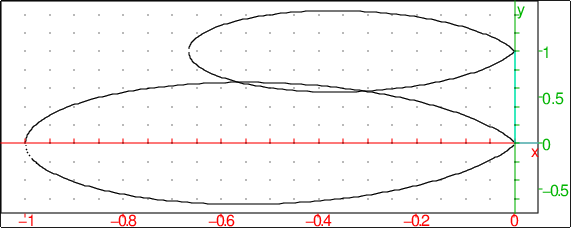
\includegraphics[width=0.75\textwidth]{xcas-catenoid_intersections.png}
\end{center}
Observe that there are exactly two catenaries satisfying the
Euler-Lagrange necessary conditions and the given boundary conditions:
the first with $K_0\approx -0.5$ and $c_1\approx 0.6$  and the second
with $K_0\approx -0.3$ and $c_1\approx 0.5$. You can obtain the values of
these constants more precisely by using \texttt{fsolve}.\\
\textit{Input:}
\begin{center}
  \texttt{p1:=fsolve([eq1,eq2],p,[-0.5,0.6]);}
  \texttt{p2:=fsolve([eq1,eq2],p,[-0.3,0.5])}
\end{center}
\textit{Output:}
\[
[-0.56237423894,0.662588703113], [-0.30613431407,0.567138261119]
\]
% \begin{center}
%   \tt [-0.56237423894,0.662588703113], [-0.30613431407,0.567138261119]
% \end{center}
You can check, for each catenary, whether the strong Legendre
condition \[f_{y'\,y'}(x,y_k,y_k')>0\] holds for $k=1,2$.\\
\textit{Input:}
\begin{center}
\begin{tabular}{l}
  \texttt{y1:=subs(y0,p,p1):; y2:=subs(y0,p,p2):;}\\
  \texttt{D2f:=diff(f,diff(y(x),x),2):;}\\
  \texttt{solve([eval(subs(D2f,y=y1,y(x)=y1))<=0,x>=0,x<=1],x);}\\
  \texttt{solve([eval(subs(D2f,y=y2,y(x)=y2))<=0,x>=0,x<=1],x)}
\end{tabular}
\end{center}
\textit{Output:}
\[
[],[]
\]
% \begin{center}
%   \tt [],[]
% \end{center}
You can conclude that the strong Legendre condition is satisfied in
both cases, so you can proceed by attempting to find the points conjugate
to 0 for each catenary. The function $y_0$ depends on two parameters,
so you can use \texttt{conjugate\_equation} to find these points
easily.\\
\textit{Input:}
\begin{center}
\begin{tabular}{l}
  \texttt{fsolve(conjugate\_equation(y0,p,p1,x,0)=0,x=0..1)}\\
  \texttt{fsolve(conjugate\_equation(y0,p,p2,x,0)=0,x=0..1)}
\end{tabular}
\end{center}
\textit{Output:}
\[
[0.0], [0.0,0.799514772606]
\]
% \begin{center}
%   \tt [0.0], [0.0,0.799514772606]
% \end{center}
You can conclude that there are no points conjugate to $0$ in $(0,1]$
for the catenary $y_1$, so it minimizes the functional $F$. However,
for the other catenary there is a conjugate point in the relevant
interval, therefore $y_2$ is not a minimizer.

You can verify the above conclusions by computing the surface area for
catenaries $y_1$ and $y_2$ and comparing them.\\
\textit{Input:}
\begin{center}
  \texttt{int(y1*sqrt(1+diff(y1,x)\^{}2),x=0..1);
  int(y2*sqrt(1+diff(y2,x)\^{}2),x=0..1)}
\end{center}
\textit{Output:}
\[
0.81396915825,0.826468466845
\]
% \begin{center}
%   \tt 0.81396915825,0.826468466845
% \end{center}
You can see that the surface formed by rotating the curve $y_1$ is
indeed smaller than the area of the surface formed by rotating the
curve $y_2$. Finally, you can visualize both surfaces for convenience.\\
\textit{Input:}\\
(see \secref{sec:plot3d} for information on \texttt{plot3d})
\begin{center}
  \texttt{plot3d([y1*cos(t),y1*sin(t),x],x=0..1,t=0..2*pi, display=yellow+filled)}
\end{center}
\textit{Output:}
\begin{center}
  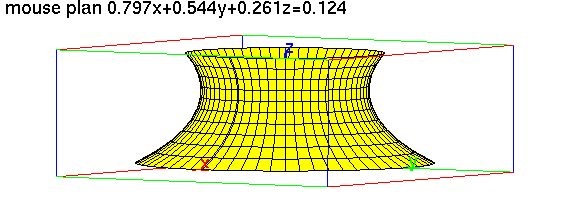
\includegraphics[width=0.75\textwidth]{xcas-catenoid_1.png}
\end{center}
\textit{Input:}
\begin{center}
  \texttt{plot3d([y2*cos(t),y2*sin(t),x],x=0..1,t=0..2*pi, display=yellow+filled)}
\end{center}
\textit{Output:}
\begin{center}
  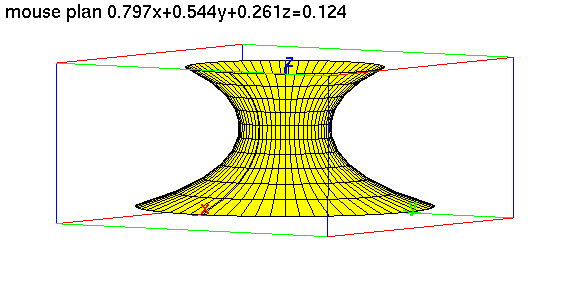
\includegraphics[width=0.75\textwidth]{xcas-catenoid_2.png}
\end{center}

\section{Trigonometry}

%\subsection{Trigonometric functions\label{sec:trigo}}

\texttt{Xcas} can evaluate the trigonometric functions in either
radians or degrees (see \secref{ssec:standardfns}).  It can also
manipulate them algebraically.

% \begin{itemize}
% \item The \texttt{sin}\index{sin} command is the sine function.
% \item The \texttt{cos}\index{cos} command is the cosine function.
% \item The \texttt{tan}\index{tan} command is the tangent function (\texttt{tan(x)=
%     sin(x)/cos(x)}).
% \item The \texttt{cot}\index{cot|textbf} command is the cotangent function (\texttt{cot(x)=
%   cos(x)/sin(x)}).
% \item The \texttt{sec}\index{sec|textbf} command is the secant function (\texttt{sec(x)=
%     1/cos(x)}).
% \item The \texttt{csc}\index{csc|textbf} command is the cosecant function (\texttt{csc(x) =
%     1/sin(x)}).
%   \item These commands take one argument: $x$, a number.\\
%   The number $x$ will by default represent an angle measured in
%   radians, but you can set \texttt{Xcas} to use degrees (see
%   \secref{ssec:angles}) by setting the variable \texttt{angle\_radian}
%   to 0; resetting it to 1 will change the angle measure to radians again.
%   \item \texttt{sin($x$)} returns the sine of $x$.\\
%   \textit{Input (with }\texttt{angle\_radian}\textit{ equal to 1):}
%   \begin{center}
%     \texttt{sin(pi/4)}
%   \end{center}
%   \textit{Output:}
%   \[
%   \frac{\sqrt{2}}{2}
%   \]
%   \textit{Input (with }\texttt{angle\_radian}\textit{ equal to 0):}
%   \begin{center}
%     \texttt{sin(30)}
%   \end{center}
%   \textit{Output:}
%   \[
%   \frac{1}{2}
%   \]
%   \item \texttt{cos($x$)} returns the cosine of $x$.\\
%   \textit{Input (with }\texttt{angle\_radian}\textit{ equal to 1):}
%   \begin{center}
%     \texttt{cos(pi/6)}
%   \end{center}
%   \textit{Output:}
%   \[
%   \frac{\sqrt{3}}{2}
%   \]
%   \textit{Input (with }\texttt{angle\_radian}\textit{ equal to 0):}
%   \begin{center}
%     \texttt{cos(90)}
%   \end{center}
%   \textit{Output:}
%   \[
%   0
%   \]
%   \item \texttt{tan($x$)} returns the tangent of $x$.\\
%   \textit{Input (with }\texttt{angle\_radian}\textit{ equal to 1):}
%   \begin{center}
%     \texttt{tan(pi/4)}
%   \end{center}
%   \textit{Output:}
%   \[
%   1
%   \]
%   \textit{Input (with }\texttt{angle\_radian}\textit{ equal to 0):}
%   \begin{center}
%     \texttt{tan(60)}
%   \end{center}
%   \textit{Output:}
%   \[
%   \sqrt{3}
%   \]
%   \item \texttt{cot($x$)} returns the cotangent of $x$.\\
%   \textit{Input (with }\texttt{angle\_radian}\textit{ equal to 1):}
%   \begin{center}
%     \texttt{cot(pi/6)}
%   \end{center}
%   \textit{Output:}
%   \[
%   \frac{2\sqrt{3}}{2}
%   \]
%   \textit{Input (with }\texttt{angle\_radian}\textit{ equal to 0):}
%   \begin{center}
%     \texttt{cot(45)}
%   \end{center}
%   \textit{Output:}
%   \[
%   1
%   \]
%   \item \texttt{sec($x$)} returns the secant of $x$.\\
%   \textit{Input (with }\texttt{angle\_radian}\textit{ equal to 1):}
%   \begin{center}
%     \texttt{sec(pi/3)}
%   \end{center}
%   \textit{Output:}
%   \[
%   2
%   \]
%   \textit{Input (with }\texttt{angle\_radian}\textit{ equal to 0):}
%   \begin{center}
%     \texttt{sec(30)}
%   \end{center}
%   \textit{Output:}
%   \[
%   \frac{2}{\sqrt{3}}
%   \]
%   \item \texttt{csc($x$)} returns the cosecant of $x$.\\
%   \textit{Input (with }\texttt{angle\_radian}\textit{ equal to 1):}
%   \begin{center}
%     \texttt{csc(pi/4)}
%   \end{center}
%   \textit{Output:}
%   \[
%   \frac{2}{\sqrt{2}}
%   \]
%   \textit{Input (with }\texttt{angle\_radian}\textit{ equal to 0):}
%   \begin{center}
%     \texttt{csc(30)}
%   \end{center}
%   \textit{Output:}
%   \[
%   2
%   \]
% \end{itemize}


% The \texttt{asin} or \texttt{arcsin}\index{asin}\index{arcsin},
% \texttt{acos} or \texttt{arccos}\index{acos}\index{arccos},
% \texttt{atan} or \texttt{arctan}\index{atan}\index{arctan},
% \texttt{acot}\index{acot|textbf}, \texttt{asec}\index{asec|textbf},
% \texttt{acsc}\index{acsc|textbf} commands are the inverse
% trigonometric functions. The latter are defined by:
% \begin{itemize}
% \item \texttt{asec(x) = acos(1/x)},
% \item
% \texttt{acsc(x) = asin(1/x)},
% \item
% \texttt{acot(x) = atan(1/x)}.
% \end{itemize}
% These functions are also among the standard functions that
% \texttt{Xcas} supports (see \secref{ssec:standardfns}).
% \begin{itemize}
%   \item These functions take one argument: $x$, a number.\\
%     They return a number which can represent an angle; by default,
%     the angles will be in radians, but you can set \texttt{Xcas} to
%     use degrees (see \secref{ssec:angles}) by setting the variable
%     \texttt{angle\_radian} to 0; resetting it to 1 will change the
%     angle measure to radians again.
%  \item \texttt{asin($x$)} (or \texttt{arcsin($x$)} returns the
%  arcsine of $x$.\\
% \textit{Input (with }\texttt{angle\_radian}\textit{ equal to 1):}
% \begin{center}
%   \texttt{asin(1/2)}
% \end{center}
% \textit{Output:}
% \[
% \frac{\pi}{6}
% \]
% \textit{Input (with }\texttt{angle\_radian}\textit{ equal to 0):}
% \begin{center}
%   \texttt{asin(1)}
% \end{center}
% \textit{Output:}
% \[
% \frac{\pi}{2}
% \]
% \item \texttt{acos($x$)} (or \texttt{arccos($x$)} returns the arccosine of $x$.\\
% \textit{Input (with }\texttt{angle\_radian}\textit{ equal to 1):}
% \begin{center}
%   \texttt{acos(sqrt(3)/2)}
% \end{center}
% \textit{Output:}
% \[
% \frac{1}{6}\pi
% \]
% \textit{Input (with }\texttt{angle\_radian}\textit{ equal to 0):}
% \begin{center}
%   \texttt{acos(-1/2)}
% \end{center}
% \textit{Output:}
% \[
% 120
% \]
% \item \texttt{atan($x$)} (or \texttt{arctan($x$)} returns the arctangent of $x$.\\
% \textit{Input (with }\texttt{angle\_radian}\textit{ equal to 1):}
% \begin{center}
%   \texttt{atan(sqrt(3))}
% \end{center}
% \textit{Output:}
% \[
% \frac{\pi}{3}
% \]
% \textit{Input (with }\texttt{angle\_radian}\textit{ equal to 1):}
% \begin{center}
%   \texttt{atan(1)}
% \end{center}
% \textit{Output:}
% \[
% 45
% \]
% \item \texttt{acot($x$)} returns the arccotangent of $x$.\\
% \textit{Input (with }\texttt{angle\_radian}\textit{ equal to 1):}
% \begin{center}
%   \texttt{acot(sqrt(3))}
% \end{center}
% \textit{Output:}
% \[
% \frac{\pi}{6}
% \]
% \textit{Input (with }\texttt{angle\_radian}\textit{ equal to 0):}
% \begin{center}
%   \texttt{acot(1/sqrt(3))}
% \end{center}
% \textit{Output:}
% \[
% 60
% \]
% \item \texttt{asec($x$)} returns the arcsecant of $x$.\\
% \textit{Input (with }\texttt{angle\_radian}\textit{ equal to 1):}
% \begin{center}
%   \texttt{asec(1)}
% \end{center}
% \textit{Output:}
% \[
% 0
% \]
% \textit{Input (with }\texttt{angle\_radian}\textit{ equal to 0):}
% \begin{center}
%   \texttt{asec(sqrt(2))}
% \end{center}
% \textit{Output:}
% \[
% 45
% \]
% \item \texttt{acsc($x$)} returns the cosecant of $x$.\\
% \textit{Input (with }\texttt{angle\_radian}\textit{ equal to 1):}
% \begin{center}
%   \texttt{acsc(1)}
% \end{center}
% \textit{Output:}
% \[
% \frac{\pi}{2}
% \]
% \textit{Input (with }\texttt{angle\_radian}\textit{ equal to 0):}
% \begin{center}
%   \texttt{acsc(2)}
% \end{center}
% \textit{Output:}
% \[
% 30
% \]
% \end{itemize}

\subsection{Expanding a trigonometric expression: \texttt{trigexpand}
\index{trigexpand}
\label{ssec:trigexpand}}

The \texttt{trigexpand} command expands sums, differences and products
by an integer inside the trigonometric functions.
\begin{itemize}
\item \texttt{trigexpand} takes one argument:\\
\textit{expr}, an expression containing trigonometric functions.
\item \texttt{trigexpand(}\textit{expr}\texttt{)} returns the
expression with sums, differences and integer products inside the trigonometric
functions expanded.
\end{itemize}
\textit{Input:}
\begin{center}
\texttt{trigexpand(cos(x+y))}
\end{center}
\textit{Output:}
\[
\cos x\cdot \cos y-\sin x\cdot \sin y
\]
%\begin{center}\texttt{cos(x)*cos(y)-sin(x)*sin(y)}\end{center}

\subsection{Linearizing a trigonometric expression: \texttt{tlin}
\index{tlin}
\label{ssec:tlin}}

The \texttt{tlin} command linearizes products and integer powers of
the trigonometric functions (e.g. in terms of $\sin(n*x)$ and
$\cos(n*x)$).
\begin{itemize}
  \item \texttt{tlin} takes one argument:\\
  \textit{expr}, an expression containing trigonometric functions.
  \item \texttt{tlin(}\textit{expr}\texttt{)} returns the expression
  with the trigonometric functions linearized.
\end{itemize}

\smallskip

\noindent
\textbf{Examples.}
\begin{itemize}
\item Linearize $\cos(x)*\cos(y)$.\\
\textit{Input:}
\begin{center}
\texttt{tlin(cos(x)*cos(y))}
\end{center}
\textit{Output:}
\[
\frac{\cos \left(x-y\right)}{2}+\frac{\cos \left(x+y\right)}{2}
\]
%\begin{center}\texttt{1/2*cos(x-y)+1/2*cos(x+y)}\end{center}
\item Linearize $\cos(x)^3$.\\
\textit{Input:}
\begin{center}
\texttt{tlin(cos(x)\^{}3)}
\end{center}
\textit{Output:}
\[
\frac{3}{4} \cos x+\frac{\cos \left(3 x\right)}{4}
\]
%\begin{center}\texttt{3/4*cos(x)+1/4*cos(3*x)}\end{center}
\item Linearize $4\cos(x)^2-2$.\\
\textit{Input:}
\begin{center}
\texttt{tlin(4*cos(x)\^{}2-2)}
\end{center}
\textit{Output:}
\[
2 \cos \left(2 x\right)
\]
%\begin{center}\texttt{2*cos(2*x)}\end{center}
\end{itemize}

\subsection{Increasing the phase by $\pi/2$ in a trigonometric expression: \texttt{shift\_phase}
\index{shift\_phase}}

The \texttt{shift\_phase} command increases the phase of a
trigonometric expression by $\pi/2$.
\begin{itemize}
  \item \texttt{shift\_phase} takes one argument:\\
  \textit{expr}, a trigonometric expression.
  \item \texttt{shift\_phase(}\textit{expr}\texttt{)} returns
  \textit{expr} with the phase increased by $\pi/2$ (after
  automatic simplification).
\end{itemize}

\smallskip

\noindent
\textbf{Examples.}
\begin{itemize}
\item \textit{Input:}
  \begin{center}
    \texttt{shift\_phase(x + sin(x))}
  \end{center}
  \textit{Output:}
  \[
  x-\cos \left(\frac{\pi +2 x}{2}\right)
  \]
%
%\begin{center}
%  \tt
% x-cos((pi+2*x)/2)
%\end{center}
  \item \textit{Input:}
  \begin{center}
    \texttt{shift\_phase(x + cos(x))}
  \end{center}
  \textit{Output:}
  \[
  x+\sin \left(\frac{\pi +2 x}{2}\right)
  \]
  % \begin{center}
  %   \tt
  %   x+sin((pi+2*x)/2)
  % \end{center}
  \item \textit{Input:}
  \begin{center}
    \texttt{shift\_phase(x + tan(x))}
  \end{center}
  \textit{Output:}
  \[
  x-\frac{1}{\tan \left(\frac{\pi +2 x}{2}\right)}
  \]
% \begin{center}
%   \tt
%  x-1/tan((pi+2*x)/2)
% \end{center}
\end{itemize}

Quoting the argument will prevent the automatic simplification.

\smallskip

\noindent
\textbf{Example.}\\
\textit{Input:}
\begin{center}
  \texttt{shift\_phase('sin(x + pi/2)')}
\end{center}
\textit{Output:}
\[
-\cos \left(\frac{\pi +2 x+2 \frac{\pi}{2}}{2}\right)
\]
% \begin{center}
%   \tt
%  -cos((pi+2*x+2*pi/2)/2)
% \end{center}
With an unquoted sine, you get:\\
\textit{Input:}
\begin{center}
  \texttt{shift\_phase(sin(x + pi/2))}
\end{center}
\textit{Output:}
\[
\sin \left(\frac{\pi +2 x}{2}\right)
\]
% \begin{center}
%   \tt
%  sin((pi+2*x)/2)
% \end{center}
since \texttt{sin(x+pi/2)} is evaluated (in this case simplified)
before \texttt{shift\_phase} is called, and
\texttt{shift\_phase(cos(x))} returns \texttt{sin((pi+2*x)/2)}.


\subsection{Putting together sine and cosine of the same angle: \texttt{tcollect} \texttt{tCollect}
\index{tcollect}
\index{tCollect}
\label{ssec:tcollect}}

The \texttt{tcollect} command linearizes
trigonometric expressions (in terms of $\sin(n*x)$ and $\cos(n*x)$) and
combines sines and cosines of the same angle.\\
\texttt{tCollect} is a synonym for \texttt{tcollect}.
\begin{itemize}
  \item \texttt{tcollect} takes one argument:\\
  \textit{expr}, an expression containing trigonometric functions.
  \item \texttt{tcollect(}\textit{expr}\texttt{)} returns \textit{expr}
  after first linearizing it and then combining sines and cosines of
  the same angle.
\end{itemize}

\smallskip

\noindent
\textbf{Examples.}
\begin{itemize}
\item \textit{Input:}
\begin{center}
\texttt{tcollect(sin(x)+cos(x))}
\end{center}
\textit{Output:}
\[
\sqrt{2} \cos \left(x-\frac{1}{4} \pi \right)
\]
%\begin{center}\texttt{sqrt(2)*cos(x-pi/4)}\end{center}
\item \textit{Input:}
\begin{center}
\texttt{tcollect(2*sin(x)*cos(x)+cos(2*x))}
\end{center}
\textit{Output:}
\[
\sqrt{2} \cos \left(2 x-\frac{1}{4} \pi \right)
\]
%\begin{center}\texttt{sqrt(2)*cos(2*x-pi/4)}\end{center}
\end{itemize}

\subsection{Simplifying: \texttt{simplify}
\index{simplify}}

The \texttt{simplify} command simplifies expressions. As with all
automatic simplifications, do not expect miracles; you will have to
use specific rewriting rules if it does not work.
\begin{itemize}
  \item \texttt{simplify} takes one argument:\\
  \textit{expr}, an expression.
  \item \texttt{simplify(}\textit{expr}\texttt{)} returns the
  simplified version of \textit{expr}.
\end{itemize}

\smallskip

\noindent
\textbf{Example.}\\
\textit{Input:}
\begin{center}
\texttt{simplify((sin(3*x)+sin(7*x))/sin(5*x))}
\end{center}
\textit{Output:}
\[
2 \cos \left(2 x\right)
\]
%\begin{center}\texttt{4*(cos(x))\^{}2-2}\end{center}

\smallskip

\noindent
\textbf{Warning.}\\
\texttt{simplify} is more efficient in \texttt{radian} mode (which you
can turn on, if it isn't already, by checking \texttt{radian} in the
\texttt{cas} configuration or inputting \texttt{angle\_radian:=1}, see
\secref{ssec:angles}).

\subsection{Simplifying trigonometric expressions: \texttt{trigsimplify}
\index{trigsimplify}}

The \texttt{trigsimplify} command simplifies trigonometric expressions
by combining \texttt{simplify} (see \secref{ssec:simplify}),
\texttt{texpand} (see \secref{ssec:texpand}), \texttt{tlin} (see
\secref{ssec:tlin}), \texttt{tcollect} (see \secref{ssec:tcollect}),
\texttt{trigsin} (see \secref{ssec:trigsin}), \texttt{trigcos} (see
\secref{ssec:trigcos}) and \texttt{trigtan} (see
\secref{ssec:trigtan}) commands in a certain order.
\begin{itemize}
  \item \texttt{trigsimplify} takes one argument:\\
  \textit{expr}, an argument containing trigonometric functions.
  \item \texttt{trigsimplify(}\textit{expr}\texttt{)} returns the
  simplified form of \textit{expr}.
\end{itemize}

\smallskip

\noindent
\textbf{Examples.}
\begin{itemize}
\item \textit{Input:}
\begin{center}
\texttt{trigsimplify((sin(x+y)-sin(x-y))/(cos(x+y)+cos(x-y)))}
\end{center}
\textit{Output:}
\[
\tan y
\]
%\begin{center}\texttt{tan(y)}\end{center}
\item \textit{Input:}
\begin{center}
\texttt{trigsimplify(1-1/4*sin(2a)\^{}2-sin(b)\^{}2-cos(a)\^{}4)}
\end{center}
\textit{Output:}
\[
\sin ^{2}a-\sin ^{2}b
\]
%\begin{center}\texttt{sin(a)\^{}2-sin(b)\^{}2}\end{center}
\end{itemize}

\subsection{Transforming arccos into arcsin: \texttt{acos2asin}
\index{acos2asin}}

The \texttt{acos2asin} command transforms any \texttt{acos}s in an
expression to \texttt{asin}s, using the identity $\arccos(x) = \pi/2 -
\arcsin(x)$.
\begin{itemize}
  \item \texttt{acos2asin} takes one argument:\\
  \texttt{expr},  an expression containing inverse trigonometric functions.
  \item \texttt{acos2asin(}\textit{expr}\texttt{)} returns
  \textit{expr} with any \texttt{acos}s replaced by the appropriate \texttt{asin}s.
\end{itemize}

\smallskip

\noindent
\textbf{Example.}\\
\textit{Input:}
\begin{center}
\texttt{acos2asin(acos(x)+asin(x))}
\end{center}
\textit{Output (after simplification):}
\[
\frac{\pi}{2}
\]
%\begin{center}\texttt{pi/2}\end{center}

\subsection{Transforming arccos into arctan: \texttt{acos2atan}
\index{acos2atan}}

The \texttt{acos2atan} command transforms any \texttt{acos}s in an
expression to \texttt{atan}s, using the identity \[ \arccos(x) =
\frac{\pi}{2} - \arctan\left(\frac{x}{\sqrt{1-x^{2}}}\right) \]
\begin{itemize}
  \item \texttt{acos2atan} takes one argument:\\
  \texttt{expr},  an expression containing inverse trigonometric functions.
  \item \texttt{acos2atan(}\textit{expr}\texttt{)} returns
  \textit{expr} with any \texttt{acos}s replaced by the appropriate \texttt{atan}s.
\end{itemize}

\smallskip

\noindent
\textbf{Example.}\\
\textit{Input:}
\begin{center}
\texttt{acos2atan(acos(x))}
\end{center}
\textit{Output:}
\[
\frac{\pi }{2}-\arctan \left(\frac{x}{\sqrt{1-x^{2}}}\right)
\]
%\begin{center}\texttt{pi/2-atan(x/sqrt(1-x\^{}2))}\end{center}

\subsection{Transforming arcsin into arccos: \texttt{asin2acos}
\index{asin2acos}}

The \texttt{asin2acos} command transforms any \texttt{asin}s in an
expression to \texttt{acos}s, using the identity $\arcsin(x) = \pi/2 -
\arccos(x)$.
\begin{itemize}
  \item \texttt{asin2acos} takes one argument:\\
  \texttt{expr},  an expression containing inverse trigonometric functions.
  \item \texttt{asin2acos(}\textit{expr}\texttt{)} returns
  \textit{expr} with any \texttt{asin}s replaced by the appropriate \texttt{acos}s.
\end{itemize}

\smallskip

\noindent
\textbf{Example.}\\
\textit{Input:}
\begin{center}
\texttt{asin2acos(acos(x)+asin(x))}
\end{center}
\textit{Output (after simplification):}
\[
\frac{\pi}{2}
\]
%\begin{center}\texttt{pi/2}\end{center}

\subsection{Transforming arcsin into arctan: \texttt{asin2atan}
\index{asin2atan}}

The \texttt{asin2atan} command transforms any \texttt{asin}s in an
expression to \texttt{atan}s, using the identity \[ \arcsin(x) =
\arctan\left(\frac{x}{\sqrt{1-x^{2}}}\right) \]
\begin{itemize}
  \item \texttt{asin2atan} takes one argument:\\
  \texttt{expr},  an expression containing inverse trigonometric functions.
  \item \texttt{asin2atan(}\textit{expr}\texttt{)} returns
  \textit{expr} with any \texttt{asin}s replaced by the appropriate \texttt{atan}s.
\end{itemize}

\smallskip

\noindent
\textbf{Example.}\\
\textit{Input:}
\begin{center}
\texttt{asin2atan(asin(x))}
\end{center}
\textit{Output:}
\[
\arctan \left(\frac{x}{\sqrt{1-x^{2}}}\right)
\]
%\begin{center}\texttt{atan(x/sqrt(1-x\^{}2))}\end{center}

\subsection{Transforming arctan into arcsin: \texttt{atan2asin}
\index{atan2asin}}

The \texttt{atan2asin} command transforms any \texttt{atan}s in an
expression to \texttt{asin}s, using the identity 
\[ \arctan(x) = \arcsin\left(\frac{x}{\sqrt{1+x^{2}}}\right) 
\]
\begin{itemize}
  \item \texttt{atan2asin} takes one argument:\\
  \texttt{expr},  an expression containing inverse trigonometric functions.
  \item \texttt{atan2asin(}\textit{expr}\texttt{)} returns
  \textit{expr} with any \texttt{atan}s replaced by the appropriate
  \texttt{asin}s.
\end{itemize}

\smallskip

\noindent
\textbf{Example.}\\
\textit{Input:}
\begin{center}
\texttt{atan2asin(atan(x))}
\end{center}
\textit{Output:}
\[
\arcsin \left(\frac{x}{\sqrt{1+x^{2}}}\right)
\]
%\begin{center}\texttt{asin(x/sqrt(1+x\^{}2))}\end{center}

\subsection{Transforming arctan into arccos: \texttt{atan2acos}
\index{atan2acos}}

The \texttt{atan2acos} command transforms any \texttt{atan}s in an
expression to \texttt{acos}s, using the identity 
\[ \arctan(x) = \frac{\pi}{2} - \arcsin\left(\frac{x}{\sqrt{1+x^{2}}}\right) 
\]
\begin{itemize}
  \item \texttt{atan2acos} takes one argument:\\
  \texttt{expr},  an expression containing inverse trigonometric functions.
  \item \texttt{atan2acos(}\textit{expr}\texttt{)} returns
  \textit{expr} with any \texttt{atan}s replaced by the appropriate
  \texttt{acos}s.
\end{itemize}

\smallskip

\noindent
\textbf{Example.}\\
\textit{Input:}
\begin{center}
\texttt{atan2acos(atan(x))}
\end{center}
\textit{Output:}
\[
\frac{\pi }{2}-\arccos \left(\frac{x}{\sqrt{1+x^{2}}}\right)
\]
%\begin{center}\texttt{pi/2-acos(x/sqrt(1+x\^{}2))}\end{center}

\subsection{Transforming complex exponentials into sin and cos: \texttt{sincos} \texttt{exp2trig}
\index{sincos}\index{exp2trig}\label{ssec:sincos}}

The \texttt{sincos} command uses the identity 
\[ 
e^{i x}=\cos(x) + i\sin(x) 
\] 
to rewrite complex exponentials in terms of sine and cosine.\\
\texttt{exp2trig} is a synonym for \texttt{sincos}.
\begin{itemize}
  \item \texttt{sincos} takes one argument:\\
  \textit{expr}, an expression containing complex exponentials.
  \item \texttt{sincos(}\textit{expr}\texttt{)} rewrites \textit{expr} in
  terms of $\sin$ and $\cos$.
\end{itemize}

\smallskip

\noindent
\textbf{Examples.}
\begin{itemize}
\item \textit{Input:}
\begin{center}
\texttt{sincos(exp(i*x))}
\end{center}
\textit{Output:}
\[
\cos x+\mathrm{i} \sin x
\]
%\begin{center}\texttt{cos(x)+(i)*sin(x)}\end{center}
\item \textit{Input:}
\begin{center}
\texttt{exp2trig(exp(-i*x))}
\end{center}
\textit{Output:}
\[
\cos x-\mathrm{i} \sin x
\]
%\begin{center}\texttt{cos(x)+(i)*(-(sin(x)))}\end{center}
\item \textit{Input:}
\begin{center}
\texttt{simplify(sincos(((i)*(exp((i)*x))\^{}2-i)/(2*exp((i)*x))))}
\end{center}
\textit{or:}
\begin{center}
\texttt{simplify(exp2trig(((i)*(exp((i)*x))\^{}2-i)/(2*exp((i)*x))))}
\end{center}
\textit{Output:}
\[
-\sin x
\]
%\begin{center}\texttt{-sin(x)}\end{center}
\end{itemize}

\subsection{Transforming tan(x) into sin(x)/cos(x): \texttt{tan2sincos}
\index{tan2sincos}}

The \texttt{tan2sincos} command replaces $\tan(x)$ by $\displaystyle
\frac{\sin(x)}{\cos(x)}$ in an expression.
\begin{itemize}
  \item \texttt{tan2sincos} takes one argument:\\
  \textit{expr}, an expression containing trigonometric functions.
  \item \texttt{tan2sincos(}\textit{expr}\texttt{)} returns
  \textit{expr} with anything of the form $\tan(x)$ replaced by $\displaystyle
  \frac{\sin(x)}{\cos(x)}$.
\end{itemize}

\smallskip

\noindent
\textbf{Example.}\\
\textit{Input:}
\begin{center}
\texttt{tan2sincos(tan(2*x))}
\end{center}
\textit{Output:}
\[
\frac{\sin \left(2 x\right)}{\cos \left(2 x\right)}
\]
%\begin{center}\texttt{sin(2*x)/cos(2*x)}\end{center}

\subsection{Transforming sin(x) into cos(x)*tan(x): \texttt{sin2costan}
\index{sin2costan}}

The \texttt{sin2costan} command replaces $\sin(x)$ by $\cos(x)\tan(x)$
in an expression.
\begin{itemize}
  \item \texttt{sin2costan} takes one argument:\\
  \textit{expr}, an expression containing trigonometric functions.
  \item \texttt{sin2costan(}\textit{expr}\texttt{)} returns
  \textit{expr} with anything of the form $\sin(x)$ replaced by
  $\cos(x)\tan(x)$.
\end{itemize}

\smallskip

\noindent
\textbf{Example.}\\
\textit{Input:}
\begin{center}
  \texttt{sin2costan(sin(2*x))}
\end{center}
\textit{Output:}
\[
\tan \left(2 x\right) \cos \left(2 x\right)
\]
% \begin{center}
%   \tt
%  tan(2*x)*cos(2*x)
% \end{center}

\subsection{Transforming cos(x) into sin(x)/tan(x): \texttt{cos2sintan}
\index{cos2sintan}}

The \texttt{cos2sintan} command replaces $\cos(x)$ by $\displaystyle
\frac{\sin(x)}{\tan(x)}$ in an expression.
\begin{itemize}
  \item \texttt{cos2sintan} takes one argument:\\
  \textit{expr}, an expression containing trigonometric functions.
  \item \texttt{cos2sintan(}\textit{expr}\texttt{)} returns
  \textit{expr} with anything of the form $\cos(x)$ replaced by $\displaystyle
  \frac{\sin(x)}{\tan(x)}$.
\end{itemize}

\smallskip

\noindent
\textbf{Example.}\\
\textit{Input:}
\begin{center}
  \texttt{cos2sintan(cos(2*x))}
\end{center}
\textit{Output:}
\[
\frac{\sin \left(2 x\right)}{\tan \left(2 x\right)}
\]
% \begin{center}
%   \tt
%  sin(2*x)/tan(2*x)
% \end{center}

\subsection{Rewriting tan(x) in terms of sin(2x) and  cos(2x): \texttt{tan2sincos2}
\index{tan2sincos2}}

The \texttt{tan2sincos2} command replaces $\tan(x)$ by $\displaystyle
\frac{\sin(2x)}{1+\cos(2x)}$ in an expression.
\begin{itemize}
  \item \texttt{tan2sincos2} takes one argument:\\
  \textit{expr}, an expression containing trigonometric functions.
  \item \texttt{tan2sincos2(}\textit{expr}\texttt{)} returns
  \textit{expr} with anything of the form $\tan(x)$ replaced by $\displaystyle
  \frac{\sin(2x)}{1+\cos(2x)}$.
\end{itemize}

\smallskip

\noindent
\textbf{Example.}\\
\textit{Input:}
\begin{center}
\texttt{tan2sincos2(tan(x))}
\end{center}
\textit{Output:}
\[
\frac{\sin \left(2 x\right)}{1+\cos \left(2 x\right)}
\]
%\begin{center}\texttt{sin(2*x)/(1+cos(2*x))}\end{center}

\subsection{Rewriting tan(x) in terms of cos(2x) and  sin(2x): \texttt{tan2cossin2}
\index{tan2cossin2}}

The \texttt{tan2cossin2} command replaces $\tan(x)$ by $\displaystyle
\frac{1-\cos(2x)}{\sin(2x)}$ in an expression.
\begin{itemize}
  \item \texttt{tan2cossin2} takes one argument:\\
  \textit{expr}, an expression containing trigonometric functions.
  \item \texttt{tan2cossin2(}\textit{expr}\texttt{)} returns
  \textit{expr} with anything of the form $\tan(x)$ replaced by $\displaystyle
  \frac{1-\cos(2x)}{\sin(2x)}$.
\end{itemize}

\smallskip

\noindent
\textbf{Example.}\\
\textit{Input:}
\begin{center}
\texttt{tan2cossin2(tan(x))}
\end{center}
\textit{Output:}
\[
\frac{1-\cos \left(2 x\right)}{\sin \left(2 x\right)}
\]
%\begin{center}\texttt{(1-cos(2*x))/sin(2*x)}\end{center}

\subsection{Rewriting sin, cos, tan in terms of tan(x/2): \texttt{halftan}
\index{halftan}\label{ssec:halftan}}

The \texttt{halftan} command rewrites the trigonometric functions in
terms of $\tan(x/2)$ using the identities:
\begin{align*}
  \sin(x) &= \frac{2\tan
  \left(\frac{x}{2}\right)}{\tan^{2}\left(\frac{x}{2}\right)+1}\\
  \cos(x) &= \frac{1-\tan^{2}\left(\frac{x}{2}\right)}
  {\tan^{2}\left(\frac{x}{2}\right)+1}\\
  \tan(x) &= \frac{2\tan\left(\frac{x}{2}\right)}{1-\tan^{2}\left(\frac{x}{2}\right)}
\end{align*}
\begin{itemize}
  \item \texttt{halftan} takes one argument:\\
  \textit{expr},  an expression containing trigonometric functions.
  \item \texttt{halftan(}\textit{expr}\texttt{)} returns \textit{expr}
  with any trigonometric functions replaced by the appropriate expression of
  \texttt{tan($x$/2)}.
\end{itemize}

\smallskip

\noindent
\textbf{Examples.}
\begin{itemize}
\item \textit{Input:}
\begin{center}
\texttt{halftan(sin(2*x)/(1+cos(2*x)))}
\end{center}
\textit{Output:}
\[
\frac{2\tan\left(\frac{2}{2} x\right)}
     {\left(\tan^{2}\left(\frac{2}{2}x\right)
       +1\right)\left(1+\frac{1-\tan^{2}\left(\frac{2}{2}x\right)}
     {\tan^{2}\left(\frac{2}{2}x\right)+1}\right)}
\]
% \begin{center}
% \begin{tabular}{l}
% \texttt{2*tan(2*x/2)/((tan(2*x/2))\^{}2+1)/}\\
% \texttt{(1+(1-(tan(2*x/2))\^{}2)/((tan(2*x/2))\^{}2+1))}
% \end{tabular}
% \end{center}
\textit{Output (after simplification with \texttt{normal(ans())}):}
\[
\tan x
\]
%\begin{center}\texttt{tan(x)}\end{center}
\item \textit{Input:}
\begin{center}
\texttt{halftan(sin(x)\^{}2+cos(x)\^{}2)}
\end{center}
\textit{Output:}
\[
\left(\frac{2 \tan \left(\frac{x}{2}\right)}
    {\tan ^{2}\left(\frac{x}{2}\right)+1}\right)^{2}+
    \left(\frac{1-\tan ^{2}\left(\frac{x}{2}\right)}
    {\tan ^{2}\left(\frac{x}{2}\right)+1}\right)^{2}
\]
% \begin{center}
% \begin{tabular}{l}
% \texttt{(2*tan(x/2)/((tan(x/2))\^{}2+1))\^{}2+}\\
% \texttt{((1-(tan(x/2))\^{}2)/((tan(x/2))\^{}2+1))\^{}2}
% \end{tabular}
% \end{center}
\textit{Output (after simplification with \texttt{normal(ans())}):}
\[
1
\]
%\begin{center}\texttt{1}\end{center}
\end{itemize}

\subsection{Rewriting trigonometric functions in terms of tan(x/2) and hyperbolic functions in terms of exp(x): \texttt{halftan\_hyp2exp}
\index{halftan\_hyp2exp}}

The \texttt{halftan\_hyp2exp} command rewrites the trigonometric
function in terms of $\tan(x/2)$ (like \texttt{halftan}, see
\secref{ssec:halftan}) and rewrites the hyperbolic functions in terms
of their definitions using exponentials, namely:
\begin{align*}
  \sinh(x) &= \frac{e^{x}-e^{-x}}{2}\\
  \cosh(x) &= \frac{e^{x}+e^{-x}}{2}\\
  \tanh(x) &= \frac{e^{x}-e^{-x}}{e^{x}+e^{-x}} =
  \frac{e^{2x}-1}{e^{2x}+1}
\end{align*}
\begin{itemize}
  \item \texttt{halftan\_hyp2exp} takes one argument:\\
   \textit{expr},  a trigonometric and hyperbolic expression.
   \item \texttt{halftan\_hyp2exp(}\textit{expr}\texttt{)} returns
   \textit{expr} with any trigonometric functions replaced by the
   appropriate expression in \texttt{tan($x$/2)} and any hyperbolic
   functions replaced by the appropriate exponentials.
\end{itemize}

\smallskip

\noindent
\textbf{Examples.}
\begin{itemize}
\item \textit{Input:}
\begin{center}
\texttt{halftan\_hyp2exp(tan(x)+tanh(x))}
\end{center}
\textit{Output:}
\[
\frac{2\tan\left(\frac{x}{2}\right)}{1-\tan ^{2}\left(\frac{x}{2}\right)}
 +\frac{\mathrm{e}^{2 x}-1}{\mathrm{e}^{2 x}+1}
\]
%\begin{center}\texttt{(2*tan(x/2))/((1-(tan(x/2))\^{}2))+(((exp(x))\^{}2-1))/ (((exp(x))\^{}2+1))}\end{center}
\item \textit{Input:}
\begin{center}
\texttt{halftan\_hyp2exp(sin(x)\^{}2+cos(x)\^{}2-sinh(x)\^{}2+cosh(x)\^{}2)}
\end{center}
\textit{Output (after simplification with \texttt{normal(ans())}):}
\[
2
\]
%\begin{center}\texttt{2}\end{center}
\end{itemize}

\subsection{Transforming trigonometric functions into complex exponentials : \texttt{trig2exp}
\index{trig2exp}\label{ssec:trig2exp}}

The \texttt{trig2exp} command replaces trigonometric functions by
their complex exponential form.
\begin{itemize}
  \item \texttt{trig2exp} takes one argument:
  \textit{expr}, an expression containing trigonometric functions.
  \item \texttt{trig2exp(}\textit{expr}\texttt{)} returns
  \textit{expr} with the trigonometric functions replaced by the
  appropriate complex exponentials ({\sc without}
  linearization).
\end{itemize}

\smallskip

\noindent
\textbf{Examples.}
\begin{itemize}
\item \textit{Input:}
\begin{center}
\texttt{trig2exp(tan(x))}
\end{center}
\textit{Output:}
\[
\frac{\left(\mathrm{e}^{\mathrm{i} x}\right)^{2}-1}{\mathrm{i} \left(\left(\mathrm{e}^{\mathrm{i} x}\right)^{2}+1\right)}
\]
%\begin{center}\texttt{((exp((i)*x))\^{}2-1)/((i)*((exp((i)*x))\^{}2+1))}\end{center}
\item \textit{Input:}
\begin{center}
\texttt{trig2exp(sin(x))}
\end{center}
\textit{Output:}
\[
\frac{\mathrm{e}^{\mathrm{i} x}-\frac1{\mathrm{e}^{\mathrm{i} x}}}{2 \mathrm{i}}
\]
%\begin{center}\texttt{(exp((i)*x)-1/(exp((i)*x)))/(2*i)}\end{center}
\end{itemize}

\subsection{Transforming inverse trigonometric functions into logarithms: \texttt{atrig2ln}
\index{atrig2ln}}

Just as the trigonometric functions can be written in terms of complex
exponentials, the inverse trigonometric functions can be written in
terms of complex logarithms.  The \texttt{atrig2ln} command does this
rewriting.
\begin{itemize}
  \item \texttt{atrig2ln} takes one argument:
  \textit{expr},  an expression containing inverse trigonometric functions.
  \item \texttt{atrig2ln(}\textit{expr}\textit{)} returns
  \textit{expr} with any inverse trigonometric functions replaced by
  the appropriate complex logarithms.
\end{itemize}

\smallskip

\noindent
\textbf{Example.}\\
\textit{Input:}
\begin{center}
\texttt{atrig2ln(asin(x))}
\end{center}
\textit{Output:}
\[
\mathrm{i} \ln \left(x+\sqrt{x^{2}-1}\right)+\frac{\pi }{2}
\]
%\begin{center}\texttt{i*log(x+sqrt(x\^{}2-1))+pi/2}\end{center}

\subsection{Simplifying and expressing preferentially with sines: \texttt{trigsin}
\index{trigsin}
\label{ssec:trigsin}}

Any trigonometric function can be written in terms of $\sin$s and
$\cos$s, and with the identity $\sin(x)^2+\cos(x)^2=1$, the even
powers of $\cos$ can be turned into powers of $\sin$.  The
\texttt{trigsin} command performs these substitutions.
\begin{itemize}
  \item \texttt{trigsin} takes one argument:\\
  \textit{expr},  an expression containing trigonometric functions.
  \item \texttt{trigsin(}\textit{expr}\texttt{)} returns \textit{expr}
  with the trigonometric functions rewritten in terms  of $\sin$ and
  $\cos$, with as many $\cos$s as possible transformed to $\sin$s.
\end{itemize}

\smallskip

\noindent
\textbf{Example.}\\
\textit{Input:}
\begin{center}
\texttt{trigsin(sin(x)\^{}4+cos(x)\^{}2+1)}
\end{center}
\textit{Output:}
\[
\sin ^{4}x-\sin ^{2}x+2
\]
%\begin{center}\texttt{sin(x)\^{}4-sin(x)\^{}2+2}\end{center}

\subsection{Simplifying and expressing preferentially with cosines: \texttt{trigcos}
\index{trigcos}
\label{ssec:trigcos}}

Any trigonometric function can be written in terms of $\sin$s and
$\cos$s, and with the identity $\sin(x)^2+\cos(x)^2=1$, the even
powers of $\sin$ can be turned into powers of $\cos$.  The
\texttt{trigcos} command performs these substitutions.
\begin{itemize}
  \item \texttt{trigcos} takes one argument:\\
  \textit{expr},  an expression containing trigonometric functions.
  \item \texttt{trigsin(}\textit{expr}\texttt{)} returns \textit{expr}
  with the trigonometric functions rewritten in terms  of $\sin$ and
  $\cos$, with as many $\sin$s as possible transformed to $\cos$s.
\end{itemize}

\smallskip

\noindent
\textbf{Example.}\\
\textit{Input:}
\begin{center}
\texttt{trigcos(sin(x)\^{}4+cos(x)\^{}2+1)}
\end{center}
\textit{Output:}
\[
\cos ^{4}x-\cos ^{2}x+2
\]
%\begin{center}\texttt{cos(x)\^{}4-cos(x)\^{}2+2}\end{center}

\subsection{Simplifying and expressing preferentially with tangents: \texttt{trigtan}
\index{trigtan}
\label{ssec:trigtan}}

The \texttt{trigtan} command rewrites trigonometric expressions into
expressions where as many trigonometric functions as possible are
written in terms of tangents, using the identities
$\sin(x)^2+\cos(x)^2=1$, $\displaystyle
\tan(x)=\frac{\sin(x)}{\cos(x)}$.
\begin{itemize}
  \item \texttt{trigtan} takes one argument:\\
  \textit{expr}, an expression containing trigonometric functions.
  \item \texttt{trigtan(}\textit{expr}\texttt{)} returns \textit{expr}
  with the trigonometric functions written as much as possible in
  terms of tangents.
\end{itemize}

\smallskip

\noindent
\textbf{Example.}\\
\textit{Input:}
\begin{center}
\texttt{trigtan(sin(x)\^{}4+cos(x)\^{}2+1)}
\end{center}
\textit{Output:}
\[
\frac{2 \tan ^{4}x+3 \tan ^{2}x+2}{\tan ^{4}x+2 \tan ^{2}x+1}
\]
%\begin{center}{\tt((tan(x))\^{}2/(1+(tan(x))\^{}2))\^{}2+1/(1+(tan(x)\^{}2)+1}\end{center}
%\textit{Output, after simplification with \texttt{normal}:}
%\begin{center}\texttt{(2*tan(x)\^{}4+3*tan(x)\^{}2+2)/(tan(x)\^{}4+2*tan(x))\^{}2+1)}\end{center}

\subsection{Rewriting an expression with different options: \texttt{convert} \texttt{convertir} \texttt{=>}
\label{ssec:convert}
\index{convert|textbf}
\index{convertir|textbf}
\index{=>}
\index{sin@{\sl sin}|textbf}
\index{cos@{\sl cos}|textbf}
\index{sincos@{\sl sincos}|textbf}
\index{exp@{\sl exp}|textbf}
\index{tan@{\sl tan}|textbf}
\index{ln@{\sl ln}|textbf}
\index{list@{\sl list}|textbf}
\index{interval@{\sl interval}|textbf}
\index{expln@{\sl expln}|textbf}
\index{string@{\sl string}|textbf}
\index{matrix@{\sl matrix}|textbf}
\index{polynom@{\sl polynom}}
\index{parfrac@{\sl parfrac}|textbf}
\index{partfrac@{\sl partfrac}|textbf}
\index{array@{\sl array}|textbf}
\index{fullparfrac@{\sl fullparfrac}|textbf}}

\texttt{Xcas} has many commands to convert expressions into different
forms; the \texttt{convert} command (or its infixed version
\texttt{=>}) is a different way to call many of these functions.
\begin{itemize}
  \item \texttt{convert} takes two or more arguments:
  \begin{itemize}
    \item \textit{expr}, an expression.
    \item \textit{option}, an option specifying which rewrite rules to
    use.  A third argument might be necessary for some options.
    Possible values of \textit{option} are:
    \begin{itemize}
    \item
     \texttt{sin}, to convert an expression like \texttt{trigsin}
     (see \secref{ssec:trigsin}).
    \item
     \texttt{cos}, to convert an expression like \texttt{trigcos}
     (see \secref{ssec:trigcos}).
    \item
     \texttt{sincos}, to convert an expression like \texttt{sincos}
     (see \secref{ssec:sincos}).
    \item
     \texttt{trig}, to convert an expression like \texttt{sincos}
     (see \secref{ssec:sincos}).
    \item
     \texttt{tan}, to convert an expression like \texttt{halftan}
     (see \secref{ssec:halftan}).
    \item
     \texttt{exp}, to convert an expression like \texttt{trig2exp}
     (see \secref{ssec:trig2exp}).
    \item
     \texttt{ln}, to convert an expression like \texttt{trig2exp}
     (see \secref{ssec:trig2exp}).
    \item
     \texttt{expln}, to convert an expression like \texttt{trig2exp}
     (see \secref{ssec:trig2exp}).
    \item
     \texttt{string}, to convert a expression into a string.
    \item
     \texttt{matrix}, to convert a list of lists into a matrix.
     \item
     \texttt{array}, to turn a table into an array (see
     \secref{ssec:spmatrices}).
    \item
     \texttt{polynom}, to convert a series (see \secref{ssec:taylor})
     into a polynomial
     by removing the remainder (see \secref{ssec:convertpoly}) or
     to convert a list representing a polynomial into a polynomial
     in internal sparse multivariate form (see
    \secref{ssec:multipoly} and \secref{ssec:polytrans}).
    \item
    \texttt{parfrac} (or \texttt{partfrac} or \texttt{fullparfrac}), to convert a rational
        function into its partial fraction decomposition (see
        \secref{ssec:convertparf}).
    \item
    \texttt{interval}, to convert an expression which evaluates to a
    number into an interval (see \secref{ssec:numb2intvl}).
    \item 
    \texttt{list} (or no argument), to convert a polynomial in
    internal sparse multivariate format (see \secref{ssec:multipoly})
    into a list.
    \item 
    \textit{unit}, a unit, to convert a unit object to a new
    compatible unit (see \secref{sec:convertunit}).
    \end{itemize}
    The values of \textit{option} that require a third argument:
    \begin{itemize}
      \item
      \texttt{contfrac}, to convert a number into a continued
      fraction.  (See \secref{ssec:convertdfc}.)  The third argument
      will be the name of a variable to store the continued fraction
      into (which must be quoted the variable was assigned).
      \item
      \texttt{base}, to convert a number into a different base
      (beginning with the units digit).  If \texttt{expr} is a number,
      then the third argument will be base to convert to (see
      \secref{sec:convertbase}), if \textit{expr} is a list of
      numbers, then the third argument will be the base to convert
      from (and \textit{expr} will be a list of the digits in this
      base, starting with the units digit).
    \end{itemize}
    Finally, if \textit{expr} is an expression with units (see
    \secref{ssec:units}), then \textit{option} can be new units to convert to
    (see \secref{sec:convertunit}).
  \end{itemize}
  \item \texttt{convert(}\textit{expr,option[,extraop]}\texttt{)}
   returns the expression with the requested conversions done.
\end{itemize}
%\end{itemize}

\smallskip

\noindent
\textbf{Examples.}
\begin{itemize}
\item \textit{Input:}
\begin{center}
\texttt{convert(1.2,confrac,'fc')}
\end{center}
\textit{Output:}
\[
\left[1,5\right]
\]
and \texttt{fc} contains the continued fraction equal to 1.2.
\item \textit{Input:}
\begin{center}
\texttt{convert(123,base,10)}
\end{center}
\textit{Output:}
\[
\left[3,2,1\right]
\]
\item \textit{Input:}
\begin{center}
\texttt{convert([3,2,1],base,10)}
\end{center}
\textit{Output:}
\[
123
\]
\item \textit{Input:}
\begin{center}
\texttt{convert(1000\_g,\_kg)}
\end{center}
\textit{Output:}
\[
1.0\;\mathrm{kg}
\]
\end{itemize}

\section{Exponentials and Logarithms}

\subsection{Rewriting hyperbolic functions as exponentials: \texttt{hyp2exp}
\index{hyp2exp}}

The hyperbolic functions are typically defined in terms of exponential
functions; the \texttt{hyp2exp} command converts hyperbolic functions
into their exponential forms.
\begin{itemize}
  \item \texttt{hyp2exp} takes one argument:\\
  \textit{expr}, an expression.
  \item \texttt{hyp2exp(}\textit{expr}\texttt{)} rewrites each
  hyperbolic function in \textit{expr} with exponentials (as a
  rational function of one exponential, i.e. \textsc{without} linearization).
\end{itemize}

\smallskip

\noindent
\textbf{Example.}\\
\textit{Input:}
\begin{center}
\texttt{hyp2exp(sinh(x))}
\end{center}
\textit{Output:}
\[
\frac{\mathrm{e}^{x}-\frac1{\mathrm{e}^{x}}}{2}
\]
%\begin{center}\texttt{(exp(x)-1/(exp(x)))/2}\end{center}

\subsection{Expanding exponentials: \texttt{expexpand}
\index{expexpand}
\label{ssec:expexpand}}

The exponential function applied to a sum can be converted into a
product of exponentials; namely,
\[
\mathrm{e}^{x+y} = \mathrm{e}^{x}\mathrm{e}^{y}
\]
The \texttt{expexpand} command does this conversion.  (For expansions
with other bases, see \secref{ssec:powexpand}.)
\begin{itemize}
  \item \texttt{expexpand} takes one argument:\\
  \textit{expr}, an expression.
  \item \texttt{expexpand(}\textit{expr}\texttt{)} returns the
  expression \textit{expr} with exponentials (base e) of sums
  rewritten as products of exponentials.
\end{itemize}

\smallskip

\noindent
\textbf{Example.}\\
\textit{Input:}
\begin{center}
\texttt{expexpand(exp(3*x)+exp(2*x+2))}
\end{center}
\textit{Output:}
\[
\left(\mathrm{e}^{x}\right)^{3}+\left(\mathrm{e}^{x}\right)^{2} \mathrm{e}^{2}
\]
%\begin{center}\texttt{exp(x)\^{}3+exp(x)\^{}2*exp(2)}\end{center}

\subsection{Expanding logarithms: \texttt{lnexpand}
\index{lnexpand}
\label{ssec:lnexpand}}

The logarithm applied to a product can be converted into a
sum of logarithms; namely,
\[
\log(x\cdot y) = \log(x) + \log(y)
\]
The \texttt{lnexpand} command does this expansion.
\begin{itemize}
  \item \texttt{lnexpand} takes one argument:\\
  \textit{expr}, an expression.
  \item \texttt{lnexpand(}\textit{expr}\texttt{)} returns the
  expression \textit{expr} with logarithms of products 
  rewritten as sums of logarithms.
\end{itemize}

\smallskip

\noindent
\textbf{Example.}\\
\textit{Input:}
\begin{center}
\texttt{lnexpand(ln(3*x\^{}2)+ln(2*x+2))}
\end{center}
\textit{Output:}
\[
\ln \left(3\right)+2 \ln \left|x\right|+\ln \left(2\right)+\ln \left(x+1\right)
\]
%\begin{center}\texttt{ln(3)+2*ln(x)+ln(2)+ln(x+1)}\end{center}

\subsection{Linearizing exponentials: \texttt{lin}
\index{lin}
\label{ssec:lin}}

The \texttt{lin} command will linearize expressions involving
exponentials; namely, it will replace products of exponentials by
exponentials of sums.  It will first replace any hyperbolic functions
by exponentials.
\begin{itemize}
  \item \texttt{lin} takes one argument:\\
  \textit{expr}, an expression.
  \item \texttt{lin(}\textit{expr}\texttt{)} returns the linearized
  version of \textit{expr}.
\end{itemize}

\smallskip

\noindent
\textbf{Examples.}
\begin{itemize}
\item
\textit{Input:}
\begin{center}
\texttt{lin(sinh(x)\^{}2)}
\end{center}
\textit{Output:}
\[
\frac{\mathrm{e}^{2 x}}{4}-\frac1{2}+\frac{\mathrm{e}^{-2 x}}{4}
\]              
%\begin{center}\texttt{1/4*exp(2*x)+1/-2+1/4*exp(-(2*x))}\end{center}
\item 
\textit{Input:}
\begin{center}
\texttt{lin((exp(x)+1)\^{}3)}
\end{center}
\textit{Output:}
\[
\mathrm{e}^{3 x}+3 \mathrm{e}^{2 x}+3 \mathrm{e}^{x}+1
\]
%\begin{center}\texttt{exp(3*x)+3*exp(2*x)+3*exp(x)+1}\end{center}
\end{itemize}

\subsection{Collecting logarithms: \texttt{lncollect}
\index{lncollect}
\label{ssec:lncollect}}

The \texttt{lncollect} command collects the logarithm in an
expression; namely, it rewrites sums of logarithms as the logarithm of
a product.
\begin{itemize}
  \item \texttt{lncollect} takes one argument:\\
   \textit{expr}, an expression.
  \item \texttt{lncollect(}\textit{expr}\texttt{)} returns
  \textit{expr} with the logarithms collected.
\end{itemize}
It may be a good idea to factor the expression with \texttt{factor}
before collecting by \texttt{lncollect}).

\smallskip

\noindent
\textbf{Examples.}
\begin{itemize}
  \item \textit{Input:}
\begin{center}
\texttt{lncollect(ln(x+1)+ln(x-1))}
\end{center}
\textit{Output:}
\[
\ln \left(\left(x+1\right) \left(x-1\right)\right)
\]
%\begin{center}\texttt{log((x+1)*(x-1))}\end{center}
\item \textit{Input:}
\begin{center}
\texttt{lncollect(exp(ln(x+1)+ln(x-1)))}
\end{center}
\textit{Output:}
\[
\left(x+1\right) \left(x-1\right)
\]
\end{itemize}
%\begin{center}\texttt{(x+1)*(x-1)}\end{center}

\smallskip

\noindent
\textbf{Warning!!!}\\
For \texttt{Xcas}, \texttt{log} is the natural logarithm, the same as
\texttt{ln}; for the base 10 logarithm, use \texttt{log10}.

\subsection{Expanding powers: \texttt{powexpand}
\index{powexpand}
\label{ssec:powexpand}}

The \texttt{powexpand} command rewrites a power of a sum as a product of
powers; it is \texttt{expexpand} (see \secref{ssec:expexpand}) with
bases other than $\mathrm{e}$.
\begin{itemize}
  \item \texttt{powexpand} takes one argument:\\
  \textit{expr}, an expression.
  \item \texttt{powexpand(}\textit{expr}\texttt{)} returns
  \textit{expr} with powers of sums replaced by sums of powers.  
\end{itemize}

\smallskip

\noindent
\textbf{Example.}\\
\textit{Input:}
\begin{center}
\texttt{powexpand(a\^{}(x+y))}
\end{center}
\textit{Output:}
\[
a^{x} a^{y}
\]
%\begin{center}\texttt{a\^{}x*a\^{}y}\end{center}


\subsection{Rewriting a power as an exponential: \texttt{pow2exp}
\index{pow2exp}
\label{ssec:pow2exp}}

Powers with arbitrary (positive) bases are often defined in terms of
exponentials with base $\mathrm{e}$ with
\[
  a^{x} = \mathrm{e}^{x \ln(a)}
\]
The \texttt{pow2exp} rewrites powers to exponentials.
\begin{itemize}
  \item \texttt{pow2exp} takes one argument:\\
   \textit{expr}, an exponential.
  \item \texttt{pow2exp(}\textit{expr}\texttt{)} returns \textit{expr}
  with any powers replaced by their corresponding exponential.
\end{itemize}

\smallskip

\noindent
\textbf{Example.}\\
\textit{Input:}
\begin{center}
\texttt{pow2exp(a\^{}(x+y))}
\end{center}
\textit{Output:}
\[
\mathrm{e}^{\left(x+y\right) \ln a}
\]
%\begin{center}\texttt{exp((x+y)*ln(a))}\end{center}

\subsection{Rewriting exp(n*ln(x)) as a power: \texttt{exp2pow}
\index{exp2pow}}

The \texttt{exp2pow} command is the inverse of \texttt{pow2exp} (see
\secref{ssec:pow2exp}).
\begin{itemize}
  \item \texttt{exp2pow} takes one argument:\\
  \textit{expr}, an expression.
  \item \texttt{exp2pow(}\textit{expr}\texttt{)} rewrites any
  subexpressions of \texttt{expr} of the form $\exp(n*\ln(x))$ as $x^{n}$.
\end{itemize}

\smallskip

\noindent
\texttt{Example.}\\
\textit{Input:}
\begin{center}
\texttt{exp2pow(exp(n*ln(x)))}
\end{center}
\textit{Output:}
\[
x^{n}
\]
%\begin{center}\texttt{x\^{}n}\end{center}

\smallskip

Note the difference with \texttt{lncollect}:
\begin{center}
\begin{tabular}{l}
  \texttt{lncollect(exp(n*ln(x))) = exp(n*log(x))}\\
  \texttt{lncollect(exp(2*ln(x))) = exp(2*log(x))}\\
  \texttt{exp2pow(exp(2*ln(x))) = x\^{}2}
\end{tabular}
\end{center}
but
\begin{center}
\begin{tabular}{l}
  \texttt{lncollect(exp(ln(x)+ln(x))) = x\^{}2}\\
  \texttt{exp2pow(exp(ln(x)+ln(x))) = x\^{}(1+1)}
\end{tabular}
\end{center}

\subsection{Simplifying complex exponentials: \texttt{tsimplify}
\index{tsimplify}}

The \texttt{tsimplify} command simplifies transcendental expressions
by rewriting the expression with complex exponentials. It is a good
idea to try other simplification instructions and call
\texttt{tsimplify} if they do not work.
\begin{itemize}
  \item \texttt{tsimplify} takes one argument:\\
  \textit{expr}, an expression.
  \item \texttt{tsimplify(}\textit{expr}\texttt{)} returns a
  (possibly) simplified version of \textit{expr}.
\end{itemize}

\smallskip

\noindent
\textbf{Example.}\\
\textit{Input:}
\begin{center}
\texttt{tsimplify((sin(7*x)+sin(3*x))/sin(5*x))}
\end{center}
\textit{Output:}
\[
\frac{\left(\mathrm{e}^{\mathrm{i} x}\right)^{4}+1}{\left(\mathrm{e}^{\mathrm{i} x}\right)^{2}}
\]
%\begin{center}\texttt{((exp((i)*x))\^{}4+1)/(exp((i)*x))\^{}2}\end{center}

\section{Rewriting transcendental and trigonometric expressions}

\subsection{Expanding transcendental and trigonometric expressions: \texttt{texpand} \texttt{tExpand}
\index{texpand|textbf}
\index{tExpand|textbf}
\label{ssec:texpand}}

The \texttt{texpand} command expands exponential
and trigonometric functions, like simultaneous calling:\\
\texttt{expexpand} (see \secref{ssec:expexpand}), which, for example,
expands $\exp(nx)$ as $\exp(x)^n$,\\ 
\texttt{lnexpand} (see \secref{ssec:lnexpand}), which, for example,
expands $\ln(x^n)$ as $n\ln(x)$ , and\\ 
\texttt{trigexpand} (see \secref{ssec:trigexpand}), which, for
example, expands $\sin(2x)$ as $2\sin(x)\cos(x)$.\\
\texttt{tExpand} is a synonym for \texttt{texpand}.
\begin{itemize}
  \item \texttt{texpand} takes one argument:\\
        \textit{expr}, an expression containing transcendental or trigonometric functions.
  \item \texttt{texpand(}\textit{expr}\texttt{)} expands these functions.
\end{itemize}

\smallskip

\noindent
\textbf{Examples.}
\begin{itemize}
\item Expand $\cos(x+y)$.\\
\textit{Input:}
\begin{center}
  \texttt{texpand(cos(x+y))}
\end{center}
\textit{Output:}
\[
\cos x\cdot \cos y-\sin x\cdot \sin y
\]
%\begin{center}\texttt{cos(x)*cos(y)-sin(x)*sin(y)}\end{center}
\item Expand $\cos(3x)$.\\
\textit{Input:}
\begin{center}
   \texttt{texpand(cos(3*x))}
\end{center}
\textit{Output:}
\[
4 \cos ^{3}x-3 \cos x
\]
%\begin{center}\texttt{4*(cos(x))\^{} 3-3*cos(x)}\end{center}
\item Expand $\displaystyle \frac{\sin(3*x)+\sin(7*x)}{\sin(5*x)}$.\\
\textit{Input:}
\begin{center}
  \texttt{texpand((sin(3*x)+sin(7*x))/sin(5*x))}
\end{center}
\textit{Output:}
\begin{gather*}
-\frac{2 \sin x}{\left(16 \cos ^{4}x-12 \cos ^{2}x+1\right) \sin x}+
\frac{28 \sin x\cdot \cos ^{2}x}{\left(16 \cos ^{4}x-12
\cos^{2}x+1\right) \sin x}-\\
\frac{80 \sin x\cdot \cos ^{4}x}{\left(16 \cos ^{4}x-
12 \cos^{2}x+1\right) \sin x}+ \frac{64 \sin x\cdot \cos ^{6}x}{\left(16 \cos ^{4}x-12 \cos ^{2}x+1\right) \sin x}
\end{gather*}
%\begin{center}\texttt{(4*(cos(x))\^{}2-1)*(sin(x)/(16*(cos(x))\^{}4- 12*(cos(x))\^{}2+1))/sin(x)+(64*(cos(x))\^{}6- 80*(cos(x))\^{}4+24*(cos(x))\^{}2-1)*sin(x)/ (16*(cos(x))\^{}4-12*(cos(x))\^{}2+1)/sin(x)}\end{center}
\textit{Output, after a simplification with \texttt{normal(ans())}:}
\[
4 \cos ^{2}x-2
\]
% \begin{center}
% \texttt{4*(cos(x))\^{}2-2}
% \end{center}
\item Expand $\exp(x+y)$.\\
\textit{Input:}
\begin{center}
\texttt{texpand(exp(x+y))}
\end{center}
\textit{Output:}
\[
\mathrm{e}^{x} \mathrm{e}^{y}
\]
%\begin{center}\texttt{exp(x)*exp(y)}\end{center}
\item Expand $\ln(x\times y)$.\\
\textit{Input:}
\begin{center}
\texttt{texpand(log(x*y))}
\end{center}
\textit{Output:}
\[
\ln y+\ln x
\]
%\begin{center}\texttt{log(x)+log(y)}\end{center}
\item Expand $\ln(x^n)$.\\
\textit{Input:}
\begin{center}
\texttt{texpand(ln(x\^{}n))}
\end{center}
\textit{Output:}
\[
n \ln x
\]
%\begin{center}\texttt{n*ln(x)}\end{center}
\item Expand $\ln((e^2)+\exp(2*\ln(2))+\exp(\ln(3)+\ln(2)))$.\\
\textit{Input:}
\begin{center}
\texttt{texpand(log(e\^{}2)+exp(2*log(2))+exp(log(3)+log(2)))}
\end{center}
\textit{Output:}
\[
6+2\cdot 3
\]
%\begin{center}\texttt{6+3*2}\end{center}
\textit{or input:}
\begin{center}
\texttt{texpand(log(e\^{}2)+exp(2*log(2)))+ lncollect(exp(log(3)+log(2)))}
\end{center}
\textit{Output:}
\[
12
\]
%\begin{center}\texttt{12}\end{center}
\item
Expand $\exp(x+y)+\cos(x+y)+\ln(3x^2)$.\\
\textit{Input:}
\begin{center}
\texttt{texpand(exp(x+y)+cos(x+y)+ln(3*x\^{}2))}
\end{center}
\textit{Output:}
\[
\cos x\cdot \cos y-\sin x\cdot \sin y+\mathrm{e}^{x} \mathrm{e}^{y}+\ln \left(3\right)+2 \ln \left|x\right|
\]
%\begin{center}\texttt{cos(x)*cos(y)-sin(x)*sin(y)+exp(x)*exp(y)+ ln(3)+2*ln(x)}\end{center}
\end{itemize}

\subsection{Combining terms of the same type: \texttt{combine}
\index{combine}\index{exp@{\sl exp}|textbf}\index{log@{\sl log}|textbf}
\index{ln@{\sl ln}|textbf}\index{sin@{\sl sin}|textbf}
\index{cos@{\sl cos}|textbf}\index{trig@{\sl trig}|textbf}}

The \texttt{combine} command joins subexpressions of various types.
\begin{itemize}
  \item \texttt{combine} takes two arguments:
  \begin{itemize}
    \item
     \textit{expr}, an expression.
    \item
    \textit{function}, the name of a function or class of
    functions.  \textit{function} can be one of \texttt{exp}, \texttt{log},
    \texttt{ln}, \texttt{sin}, \texttt{cos}, or \texttt{trig}.
  \end{itemize}
  \item \texttt{combine(}\textit{expr,function}\texttt{)} returns the
  expression with subexpressions corresponding to the second argument
  combined.
\end{itemize}
The \texttt{combine} command can duplicate the effect of other commands.
\begin{itemize}
\item \texttt{combine(}\textit{expr}\texttt{,ln)} or
\texttt{combine(}\textit{expr}\texttt{,log)} gives the same result
  as \texttt{lncollect(}\textit{expr}\texttt{)} (see
  \secref{ssec:lncollect}).
\item \texttt{combine(}\textit{expr}\texttt{,trig)} or
\texttt{combine(}\textit{expr}\texttt{,sin)}  or
\texttt{combine(}\textit{expr}\textit{,cos)}
gives the same result as \texttt{tcollect(}\textit{expr}\texttt{)}
(see \secref{ssec:tcollect}).
\end{itemize}

\smallskip

\noindent
\textbf{Examples.}
\begin{itemize}
  \item \textit{Input:}
\begin{center}
\texttt{combine(exp(x)*exp(y)+sin(x)*cos(x)+ln(x)+ln(y),exp)}
\end{center}
\textit{Output:}
\[
\cos x\cdot \sin x+\ln x+\ln y+\mathrm{e}^{x+y}
\]
%\begin{center}\texttt{exp(x+y)+sin(x)*cos(x)+ln(x)+ln(y)}\end{center}
\item \textit{Input:}
\begin{center}
\texttt{combine(exp(x)*exp(y)+sin(x)*cos(x)+ln(x)+ln(y),trig)}
\end{center}
\textit{or:}
\begin{center}
\texttt{combine(exp(x)*exp(y)+sin(x)*cos(x)+ln(x)+ln(y),sin)}
\end{center}
\textit{or:}
\begin{center}
\texttt{combine(exp(x)*exp(y)+sin(x)*cos(x)+ln(x)+ln(y),cos)}
\end{center}
\textit{Output:}
\[
\mathrm{e}^{x} \mathrm{e}^{y}+\ln x+\ln y+\frac{\sin \left(2 x\right)}{2}
\]
%\begin{center}\texttt{exp(y)*exp(x)+(sin(2*x))/2+ln(x)+ln(y)}\end{center}
\item \textit{Input:}
\begin{center}
\texttt{combine(exp(x)*exp(y)+sin(x)*cos(x)+ln(x)+ln(y),ln)}
\end{center}
\textit{or:}
\begin{center}
\texttt{combine(exp(x)*exp(y)+sin(x)*cos(x)+ln(x)+ln(y),log)}
\end{center}
\textit{Output:}
\[
\cos x\cdot \sin x+\mathrm{e}^{x} \mathrm{e}^{y}+\ln \left(x y\right)
\]
%\begin{center}\texttt{exp(x)*exp(y)+sin(x)*cos(x)+ln(x*y)}\end{center}
\end{itemize}

\section{Fourier transformation}

\subsection{Fourier coefficients: \texttt{fourier\_an} and  \texttt{fourier\_bn} or \texttt{fourier\_cn}
\index{integer}}

Let $f$ be a $T$-periodic continuous function on $\mathbb{R}$ except
perhaps at a finite number of points. One can prove that if $f$ is
continuous at $x$, then;
\begin{align*}
f(x)&= \frac{a_0}{2}+\sum _{n=1}^{+\infty} a_n \cos(\frac{2\pi
  nx}{T})+b_n \sin(\frac{2\pi nx}{T}) \\
 &= \sum _{n=-\infty}^{+\infty} c_n e^{\frac{2i\pi nx}{T}}
\end{align*}
where the coefficients $a_n,\ b_n$, $n\in N$, (or $c_n$, $n \in Z$) are the
Fourier coefficients of $f$.
The \texttt{fourier\_an} and \texttt{fourier\_bn} or
\texttt{fourier\_cn} commands compute these coefficients.

\subsubsection{\texttt{fourier\_an}\label{sssec:fourier_an}
\index{fourier\_an}}

\begin{itemize}
  \item \texttt{fourier\_an} takes four mandatory and one optional argument:
  \begin{itemize}
    \item \textit{expr}, an expression depending on a variable.
    \item $x$, the name of this variable.
    \item $T$, the period.
    \item $n$, a non-negative integer.
    \item Optionally, $a$ a real number (by default $a=0$).
  \end{itemize}
  \item \
  \texttt{fourier\_an(}\textit{expr}\texttt{,$x,T,n\,\langle,a\rangle$)} returns the
  Fourier coefficient $a_n$ of a function $f$ of variable $x$ defined on
  $[a,a+T)$ by $f(x)=$\textit{expr} and such that $f$ is
  periodic with period $T$:
\[
   a_n=\frac{2}{T}\int_a^{a+T}f(x)\cos(\frac{2\pi nx}{T})dx
\]
\end{itemize}
To simplify the computations, you should input \texttt{assume(n,integer)}
(see \secref{ssec:about}) before calling \texttt{fourier\_an} with an
unspecified \texttt{n} to specify that it is an integer.

\smallskip

\noindent
\textbf{Example.}\\
Let the function $f$, with period $T=2$, be defined on $[-1,1)$ by $f(x)=x^2$.\\
\textit{Input (to have the coefficient $a_0$):}
\begin{center}
\texttt{fourier\_an(x\^{}2,x,2,0,-1)}
\end{center}
\textit{Output:}
\[
\frac{1}{3}
\]
%\begin{center}\texttt{1/3}\end{center}
\textit{Input (to have the coefficient $a_n$ ($n\neq 0$)):}
\begin{center}
\begin{tabular}{l}
  \texttt{assume(n,integer)}\\
  \texttt{fourier\_an(x\^{}2,x,2,n,-1)}
\end{tabular}
\end{center}
\textit{Output:}
\[
\frac{4 \left(-1\right)^{n}}{n^{2} \pi ^{2}}
\]
%\begin{center}\texttt{4*(-1)\^{}n/(pi\^{}2*n\^{}2)}\end{center}

\subsubsection{\texttt{fourier\_bn}\label{sssec:fourier_bn}
\index{fourier\_bn}}

\begin{itemize}
  \item \texttt{fourier\_bn} takes four mandatory and one optional argument:
  \begin{itemize}
    \item \textit{expr}, and expression depending on a variable.
    \item $x$, the name of this variable.
    \item $T$, the period.
    \item $n$, an integer.
    \item Optionally, $a$ a real number (by default $a=0$).
  \end{itemize}
  \item \
  \texttt{fourier\_bn(}\textit{expr}\texttt{$,x,T,n\,\langle,a\rangle$)} returns the
  Fourier coefficient $b_n$ of a function $f$ of variable $x$ defined on
  $[a,a+T)$ by $f(x)=$\textit{expr} and such that $f$ is
  periodic with period $T$:
\[
   b_n=\frac{2}{T}\int_a^{a+T}f(x)\sin(\frac{2\pi nx}{T})dx
\]
\end{itemize}
To simplify the computations, you should input \texttt{assume(n,integer)}
(see \secref{ssec:about}) before calling \texttt{fourier\_bn} to
specify that $n$ is an integer.

\smallskip

\noindent 
\textbf{Examples.}
\begin{itemize}
\item Let the function $f$, with period $T=2$, defined on $[-1,1)$ by
$f(x)=x^2$.\\
\textit{Input (to get the coefficient $b_n$ ($n\neq 0$)):}
\begin{center}
\begin{tabular}{l}
  \texttt{assume(n,integer)}\\
  \texttt{fourier\_bn(x\^{}2,x,2,n,-1)}
\end{tabular}
\end{center}
\textit{Output:}
\[
0
\]
%\begin{center}\texttt{0}\end{center}
\item Let the function $f$, with period $T=2$, defined on $[-1,1)$ by
$f(x)=x^3$.\\
\textit{Input (to get the coefficient  $b_1$):}
 \begin{center}
 \texttt{fourier\_bn(x\^{}3,x,2,1,-1)}
 \end{center}
\textit{Output:}
\[
\frac{2 \pi ^{2}-12}{\pi ^{3}}
\]
%\begin{center}\texttt{(2*pi\^{}2-12)/pi\^{}3}\end{center}
\end{itemize}

\subsubsection{\texttt{fourier\_cn}\label{sssec:fourier_cn}
\index{fourier\_cn}}

\begin{itemize}
  \item \texttt{fourier\_cn} takes four mandatory and one optional argument:
  \begin{itemize}
    \item \textit{expr}, and expression depending on a variable.
    \item $x$, the name of this variable.
    \item $T$, the period.
    \item $n$, an integer.
    \item Optionally, $a$ a real number (by default $a=0$).
  \end{itemize}
  \item \
  \texttt{fourier\_cn(}\textit{expr}\texttt{,$x,T,n\,\langle,a\rangle$)} returns the
  Fourier coefficient $c_n$ of a function $f$ of variable $x$ defined on
  $[a,a+T)$ by $f(x)=$\textit{expr} and such that $f$ is
  periodic with period $T$:
\[
   c_n=\frac{1}{T}\int_a^{a+T}f(x)e^{\frac{-2i\pi nx}{T}}dx
\]
\end{itemize}
To simplify the computations, you should input \texttt{assume(n,integer)}
(see \secref{ssec:about}) before calling \texttt{fourier\_cn} to
specify that $n$ is an integer.

\smallskip

\noindent \textbf{Examples.}
\begin{itemize}
\item Find the Fourier coefficients $c_n$ of the periodic function $f$ of
period $2$ and  defined on $[-1,1)$ by $ f(x)=x^2$.\\
\textit{Input (to get $c_0$):}
\begin{center}
\texttt{fourier\_cn(x\^{}2,x,2,0,-1)}
\end{center}
\textit{Output:}
\[
\frac{1}{3}
\]
%\begin{center}\texttt{1/3}\end{center}
\textit{Input (to get $c_n$):}
\begin{center}
\begin{tabular}{l}
  \texttt{assume(n,integer)}\\
  \texttt{fourier\_cn(x\^{}2,x,2,n,-1)}
\end{tabular}
\end{center}
\textit{Output:}
\[
\frac{2 \left(-1\right)^{n}}{n^{2} \pi ^{2}}
\]
%\begin{center}\texttt{2*(-1)\^{}n/(pi\^{}2*n\^{}2)}\end{center}
\item Find the Fourier coefficients $c_n$ of the periodic function $f$, of
period $2$, and defined on $[0,2)$ by $ f(x)=x^2$.\\
\textit{Input (to have $c_0$):}
\begin{center}
\texttt{fourier\_cn(x\^{}2,x,2,0)}
\end{center}
\textit{Output:}
\[
\frac{4}{3}
\]
%\begin{center}\texttt{4/3}\end{center}
\textit{Input (to get $c_n$):}
\begin{center}
\begin{tabular}{l}
  \texttt{assume(n,integer)}\\
  \texttt{fourier\_cn(x\^{}2,x,2,n)}
\end{tabular}
\end{center}
\textit{Output:}
\[
\frac{\pi \cdot 2 \mathrm{i} n+2}{n^{2} \pi ^{2}}
\]
%\begin{center}\texttt{((2*i)*pi*n+2)/(pi\^{}2*n\^{}2)}\end{center}

\item Find the Fourier coefficients $c_n$ of the periodic function $f$ of
period $2\pi$ and  defined on $[0,2\pi)$ by $ f(x)=x^2$.\\
\textit{Input:}
\begin{center}
\begin{tabular}{l}
\texttt{assume(n,integer)}\\
\texttt{fourier\_cn(x\^{}2,x,2*pi,n)}
\end{tabular}
\end{center}
\textit{Output:}
\[
\frac{\pi \cdot 2 \mathrm{i} n+2}{n^{2}}
\]
%\begin{center}\texttt{((2*i)*pi*n+2)/n\^{}2}\end{center}
% If you don't specify \texttt{assume(n,integer)}, the output will not be
% simplified:\\
% \textit{Input:}
% \begin{center}
% \begin{tabular}{l}
% \textit{purge(n)}\\
% \texttt{fourier\_cn(x\^{}2,x,2*pi,n)}
% \end{tabular}
% \end{center}
% \textit{Output:}
% \[
% \frac{\pi \cdot 2 \mathrm{i} n+2}{n^{2}}
% \frac{\pi \cdot 2 \mathrm{i} n+2}{n^{2}}
% \]
% \begin{center}
% \texttt{(-i)*exp((-i)*n*2*pi)+i)/(pi*n\^{}3)}
% \end{center}
% You might simplify this expression by replacing
% \texttt{exp((-i)*n*2*pi)} by \texttt{1}:
% \textit{Input:}
% \begin{center}\texttt{subst(ans(),exp((-i)*n*2*pi)=1)}\end{center}
% \textit{Output:}
% \begin{center}\texttt{((2*i)*pi\^{}2*n\^{}2+2*pi*n+-i+i)/pi/n\^{}3}\end{center}
% This expression is then simplified with \texttt{normal}, the final
% output is:
% \begin{center}\texttt{((2*i)*pi*n+2)/n\^{}2}\end{center}
% Hence for $n \neq 0$, $\displaystyle c_n=\frac{2in\pi+2}{n^2}$.
% As shown in this example, it is better to input  {\tt
%   assume(n,integer)} before calling \texttt{fourier\_cn}.\\
You must also compute $c_n$ for $n=0$:
\textit{Input:}
\begin{center}
\texttt{fourier\_cn(x\^{}2,x,2*pi,0)}
\end{center}
\textit{Output:}
\[
\frac{4}{3} \pi ^{2}
\]
%\begin{center}\texttt{4*pi\^{}2/3}\end{center}
Hence for  $n= 0$, $\displaystyle c_0=\frac{4{\pi}^2}{3}$.
\end{itemize}

\smallskip

\noindent \textbf{Remarks.}
\begin{itemize}
\item Input \texttt{purge(n)}\index{purge} (see \secref{ssec:VARS}) to
remove the hypothesis done on $n$.
\item
Input \texttt{about(n)}\index{about} or \texttt{assume(n)}\index{assume}, to know
the hypothesis done on the variable $n$.
\end{itemize}

\subsection{Continuous Fourier Transform: \texttt{fourier} \texttt{ifourier} \texttt{addtable}
\index{fourier}
\index{ifourier}
\index{addtable}
\label{ssec:cfourier}}

The Fourier transform of a function $f$ is defined by
\begin{equation}\label{eq:fourier-def}
F(s)=\int_{-\infty}^{+\infty}\mathrm{e}^{-\mathrm{i}\,s\,x}\,f(x)\,\mathrm{d}x,\quad s\in\mathbb{R}.
\end{equation}
The \texttt{fourier} command computes the Fourier transform.
\begin{itemize}
  \item \texttt{fourier} takes one mandatory argument and two optional
  arguments:
  \begin{itemize}
    \item \textit{expr}, an expression which defines a function
    $f(x)=$\textit{expr}.
    \item Optionally, $x$, the variable for $f$ (by default
    \texttt{x}).
    \item Optionally, $s$, the variable for the Fourier
    transform (by default $x$).
  \end{itemize}
  \item \texttt{fourier(}\textit{expr}$\,\langle ,x,s\rangle$)\texttt{} returns
  the Fourier transform $F(s)$.  If $s$
  is not given, then $x$ will be used.
\end{itemize}

The inverse Fourier transform, as its name implies, takes a Fourier
transform $F(x)$ and returns the original function $f(x)$.  It is
given by:
\begin{equation}\label{eq:ifourier-def}
f(x)=\frac{1}{2\,\pi}\,\int_{-\infty}^{+\infty}\mathrm{e}^{\mathrm{i}\,s\,x}\,F(s)\,\mathrm{d}s.
\end{equation}
The \texttt{ifourier} command computes the inverse Fourier transform.
\begin{itemize}
  \item \texttt{ifourier} takes one mandatory argument and two optional
  arguments:
  \begin{itemize}
    \item \textit{expr}, an expression which defines a function
    $F(x)=$\textit{expr}.
    \item Optionally, $x$, the variable for $F$ (by default
    \texttt{x}).
    \item Optionally, $X$, the variable for the original
    function $f$ (by default $x$).
  \end{itemize}
  \item \texttt{ifourier(}\textit{expr}$\,\langle ,x,X\rangle$\texttt{)} returns
  the inverse Fourier transform $f(X)$.  If $X$
  is not given, then $x$ will be used.
\end{itemize}

Note the similarity between the definitions of the Fourier transform
(equation \eqref{eq:fourier-def}) and its inverse (equation
\eqref{eq:ifourier-def}).  To compute the inverse transformation of
$F(s)$, it is enough to compute the Fourier transform with function
$\frac{F(s)}{2\pi}$ and using the variables $s$ and $x$ instead of $x$
and $s$, and replacing $x$ with $-x$ in the result.

Arbitrary rational functions can be transformed.\\

\smallskip

\noindent
\textbf{Examples.}
\begin{itemize}
\item Find the Fourier transform of $f(x)=\frac{x}{x^3-19\,x+30}$:\\
\textit{Input:}
\begin{center}
  \texttt{F:=fourier(x/(x\^{}3-19x+30),x,s)}
\end{center}
\textit{Output:}
\[
\frac{1}{56} \pi  \mathrm{sign}\left(s\right) \left(16 \mathrm{i} \mathrm{e}^{-2 \mathrm{i} s}
   -21 \mathrm{i} \mathrm{e}^{-3 \mathrm{i} s}
   +5 \mathrm{i} \mathrm{e}^{5 \mathrm{i} s}\right)
\]
% \begin{center}
%   \tt pi*(5*i*exp(5*i*s)+(-21*i)*exp((-3*i)*s)+16*i*exp((-2*i)*s))*sign(s)/56
% \end{center}
\textit{Input:}
\begin{center}
  \texttt{ifourier(F,s,x)}
\end{center}
\textit{Output:}
\[
\frac{x}{x^{3}-19 x+30}
\]
% \begin{center}
%   \tt x/(x\^{}3-19*x+30)
% \end{center}
\item Find the transform of $ f(x)=\frac{x^2+1}{x^2-1}$:\\
\textit{Input:}
\begin{center}
  \texttt{F:=fourier((x\^{}2+1)/(x\^{}2-1),x,s)}
\end{center}
\textit{Output:}
\[
2 \pi  \left(\operatorname{\delta}\left(s\right)-\mathrm{sign}\left(s\right) \sin s\right)
\]
% \begin{center}
%   \tt 2*pi*(Dirac(s)-sign(s)*sin(s))
% \end{center}
\textit{Input:}
\begin{center}
  \texttt{ifourier(F,s,x)}
\end{center}
\textit{Output:}
\[
\frac{x^{2}+1}{x^{2}-1}
\]
% \begin{center}
%   \tt (x\^{}2+1)/(x\^{}2-1)
% \end{center}
\end{itemize}

A range of other (generalized) functions and distributions can be
transformed, as demonstrated in the following examples. If
\texttt{fourier} does not know how to transform a function, it returns
the unevaluated integral~\eqref{eq:fourier-def}. In these cases you
may try to evaluate the result using \texttt{eval}.

\smallskip

\noindent
\textbf{Examples.}
\begin{itemize}
\item \textit{Input:}
\begin{center}
  \texttt{fourier(3x\^{}2+2x+1,x,s)}
\end{center}
\textit{Output:}
\[
2 \pi  \left(\operatorname{\delta}\left(s\right)+2 \mathrm{i} \operatorname{\delta}\left(s,1\right)-3 \operatorname{\delta}\left(s,2\right)\right)
\]
% \begin{center}
%   \tt 2*pi*(Dirac(s)+2*i*Dirac(s,1)-3*Dirac(s,2))
% \end{center}
\item \textit{Input:}
\begin{center}
  \texttt{fourier(Dirac(x-1)+Dirac(x+1),x,s)}
\end{center}
\textit{Output:}
\[
2 \cos s
\]
% \begin{center}
%   \tt 2*cos(s)
% \end{center}
\item \textit{Input:}
\begin{center}
  \texttt{fourier(exp(-2*abs(x-1)),x,s)}
\end{center}
\textit{Output:}
\[
\frac{4 \mathrm{e}^{-\mathrm{i} s}}{s^{2}+4}
\]
% \begin{center}
%   \tt 4*exp(-i*s)/(s\^{}2+4)
% \end{center}
\item \textit{Input:}
\begin{center}
  \texttt{fourier(atan(1/(2x\^{}2)),x,s)}
\end{center}
\textit{Output:}
\[
\frac{2 \pi  \mathrm{e}^{-\frac{\left|s\right|}{2}} \sin \left(\frac{s}{2}\right)}{s}
\]
\begin{center}
  \tt 2*pi*sin(s/2)*exp(-abs(s)/2)/s
\end{center}
\item \textit{Input:}
\begin{center}
  \texttt{fourier(BesselJ(3,x),x,s)}
\end{center}
\textit{Output:}
\[
-\frac{s \left(4 s^{2}-3\right) \left(-\mathrm{i} \mathrm{sign}\left(s+1\right)+\mathrm{i} \mathrm{sign}\left(s-1\right)\right)}{\sqrt{-s^{2}+1}}
\]
% \begin{center}
%   \tt -s*(4*s\^{}2-3)*(-i*sign(s+1)+i*sign(s-1))/sqrt(-s\^{}2+1)
% \end{center}
\item \textit{Input:}
\begin{center}
  \texttt{F:=fourier(sin(x)*sign(x),x,s)}
\end{center}
\textit{Output:}
\[
-\frac{2}{s^{2}-1}
\]
% \begin{center}
%   \tt -2/(s\^{}2-1)
% \end{center}
\textit{Input:}
\begin{center}
  \texttt{ifourier(F,s,x)}
\end{center}
\textit{Output:}
\[
\mathrm{sign}\left(x\right) \sin x
\]
% \begin{center}
%   \tt sign(x)*sin(x)
% \end{center}
\item \textit{Input:}
\begin{center}
  \texttt{fourier(log(abs(x)),x,s)}
\end{center}
\textit{Output:}
\[
-\frac{\pi  \left(2 \gamma  \operatorname{\delta}\left(s\right) \left|s\right|+1\right)}{\left|s\right|}
\]
% \begin{center}
%   \tt -pi*(2*euler\_gamma*Dirac(s)*abs(s)+1)/abs(s)
% \end{center}
\item \textit{Input:}
\begin{center}
  \texttt{fourier(rect(x),x,s)}
\end{center}
\textit{Output:}
\[
\frac{2 \sin \left(\frac{s}{2}\right)}{s}
\]
% \begin{center}
%   \tt 2*sin(s/2)/s
% \end{center}
\item \textit{Input:}
\begin{center}
  \texttt{fourier(exp(-abs(x))*sinc(x),x,s)}
\end{center}
\textit{Output:}
\[
\arctan \left(s+1\right)-\arctan \left(s-1\right)
\]
% \begin{center}
%   \tt atan(s+1)-atan(s-1)
% \end{center}
\item \textit{Input:}
\begin{center}
  \texttt{fourier(1/sqrt(abs(x)),x,s)}
\end{center}
\textit{Output:}
\[
\frac{\sqrt{2} \sqrt{\pi }}{\sqrt{\left|s\right|}}
\]
% \begin{center}
%   \tt sqrt(2)*sqrt(pi)/sqrt(abs(s))
% \end{center}
\item \textit{Input:}
\begin{center}
  \texttt{F:=fourier(1/cosh(2x),x,s)}
\end{center}
\textit{Output:}
\[
\frac{\pi }{\mathrm{e}^{-\frac{1}{4} \pi  s}+\mathrm{e}^{\frac{1}{4} \pi  s}}
\]
% \begin{center}
%   \tt pi/(exp(pi*s/4)+exp(-pi*s/4))
% \end{center}
\textit{Input:}
\begin{center}
  \texttt{ifourier(F,s,x)}
\end{center}
\textit{Output:}
\[
\frac{2}{\mathrm{e}^{-2 x}+\mathrm{e}^{2 x}}
\]
% \begin{center}
%   \tt 2/(exp(2*x)+exp(-2*x))
% \end{center}
\item \textit{Input:}
\begin{center}
  \texttt{fourier(Airy\_Ai(x/2),x,s)}
\end{center}
\textit{Output:}
\[
2 \mathrm{e}^{\frac{8}{3} \mathrm{i} s^{3}}
\]
% \begin{center}
%   \tt 2*exp(8*i*s\^{}3/3)
% \end{center}
\item \textit{Input:}
\begin{center}
  \texttt{F:=fourier(Gamma(1+i*x/3),x,s)}
\end{center}
\textit{Output:}
\[
6 \pi  \mathrm{e}^{-\left(3 s+\mathrm{e}^{-3 s}\right)}
\]
% \begin{center}
%   \tt 6*pi*exp(-exp(-3*s)-3*s)
% \end{center}
\textit{Input:}
\begin{center}
  \texttt{ifourier(F,s,x)}
\end{center}
\textit{Output:}
\[
\Gamma\left(\frac{1}{3} \mathrm{i} x+1\right)
\]
% \begin{center}
%   \tt Gamma(i*x/3+1)
% \end{center}
\item \textit{Input:}
\begin{center}
  \texttt{F:=fourier(atan(x/4)/x,x,s)}
\end{center}
\textit{Output:}
\[
\pi  \mathrm{ugamma}\left(0,4 \left|s\right|\right)
\]
% \begin{center}
%   \tt pi*ugamma(0,4*abs(s))
% \end{center}
\textit{Input:}
\begin{center}
  \texttt{ifourier(F,s,x)}
\end{center}
\textit{Output:}
\[
\frac{\arctan \left(\frac{x}{4}\right)}{x}
\]
% \begin{center}
%   \tt atan(x/4)/x
% \end{center}
\item \textit{Input:}
\begin{center}
\begin{tabular}{l}
  \texttt{assume(a>0)}\\
  \texttt{fourier(exp(-a*x\^{}2+b),x,s)}
\end{tabular}
\end{center}
\textit{Output:}
\[
\frac{\sqrt{a} \sqrt{\pi } \mathrm{e}^{-\frac{s^{2}}{4 a}+b}}{a}
\]
% \begin{center}
%   \tt sqrt(a)*sqrt(pi)*exp(-s\^{}2/(4*a)+b)/a
% \end{center}
\end{itemize}

The Fourier transform behaves nicely when combined with convolutions.
Recall the \emph{convolution} (see \secref{ssec:convolution}) of two
functions $f$ and $g$ is 
\[ 
(f\ast g)(x) = \int_{-\infty}^{+\infty}f(t)\,g(x-t)\,\mathrm{d}t 
\] 
If $\mathcal{F}(f)$ represents the Fourier transform of a function $f$,
then the convolution theorem states 
\[ 
\mathcal{F}(f\ast g) = \mathcal{F}(f)\cdot\mathcal{F}(g). 
\] 

\smallskip

\noindent
\textbf{Example.}\\
In this example, the convolution theorem will be used to compute the
convolution of $f(x)=\mathrm{e}^{-|x|} $ with itself.\\ 
\textit{Input:}
\begin{center}
  \texttt{F:=fourier(exp(-abs(x)),x,s)}
\end{center}
\textit{Output:}
\[
\frac{2}{s^{2}+1}
\]
% \begin{center}
%   \tt 2/(s\^{}2+1)
% \end{center}
\textit{Input:}
\begin{center}
  \texttt{ifourier(F\^{}2,s,x)}
\end{center}
\textit{Output:}
\[
-x \operatorname{\theta}\left(-x\right) \mathrm{e}^{x}+x \operatorname{\theta}\left(x\right) \mathrm{e}^{-x}+\mathrm{e}^{-\left|x\right|}
\]
% \begin{center}
%   \tt x*Heaviside(x)*exp(-x)-x*Heaviside(-x)*exp(x)+exp(-abs(x))
% \end{center}
The above result is the desired convolution
$(f\ast f)(x)=\int_{-\infty}^{+\infty}f(t)\,f(x-t)\,\mathrm{d}t$.

\smallskip

Piecewise functions can be transformed if defined as
\begin{center}
  \texttt{piecewise(}$x<a_{1},f_{1},x<a_{2},f_{2},\ldots,x<a_{n},f_{n},f_{0}$\texttt{)}
\end{center}
for appropriate functions $f_{0},\ldots,f_{n}$
and $a_1,a_2,\dots,a_n $ are real numbers such that 
$a_1<a_2<\cdots<a_n $. Inequalities may be strict or non-strict.

\smallskip

\noindent
\textbf{Example.}\\
\textit{Input:}
\begin{center}
\begin{tabular}{l}
  \texttt{f:=piecewise(x<=-1,exp(x+1),x<=1,1,exp(2-2x))}\\
  \texttt{F:=fourier(f,x,s)}
\end{tabular}
\end{center}
\textit{Output:}
\[
\frac{3 s \cos s-\mathrm{i} s \sin s+4 \sin s}{s \left(s-2 \mathrm{i}\right) \left(s+\mathrm{i}\right)}
\]
% \begin{center}
%   \tt (-i*s*sin(s)+3*s*cos(s)+4*sin(s))/(s*(s-2*i)*(s+i))
% \end{center}
You can obtain the original function $f$ from the above result by
applying \texttt{ifourier}.\\
\textit{Input:}
\begin{center}
  \texttt{ifourier(F,s,x)}
\end{center}
\textit{Output:}
\[
\operatorname{\theta}\left(-x-1\right) \mathrm{e}^{x+1}+\operatorname{\theta}\left(x+1\right)+\operatorname{\theta}\left(x-1\right) \mathrm{e}^{-2 x+2}-\operatorname{\theta}\left(x-1\right)
\]
% \begin{center}
%   \tt Heaviside(x+1)-Heaviside(x-1)+Heaviside(x-1)*exp(-2*x+2)+ Heaviside(-x-1)*exp(x+1)
% \end{center}
You can verify that the above expression is equal to $f(x)$ by
plotting them.

\smallskip

Some algebraic transformations of a function behave predictably under
the Fourier transform.  For example, if $g(x) = f(x-a)$, then
$\mathcal{F}(g)(s) = e^{-2\pi i a s}\mathcal{F}(f)(s)$.  The
\texttt{addtable} command lets you assign a function name to the
Fourier (or Laplace\index{laplace}, see \secref{ssec:laplace})
transform of another function name, without specifying the either
function.  This allows you to alter the original function and see the
effect on the Fourier (or Laplace) transform.
\begin{itemize}
  \item \texttt{addtable}\index{addtable} takes five arguments:
  \begin{itemize}
    \item \textit{transform}, which can be \texttt{fourier} or
    \texttt{laplace} and indicates the type of transform.
    \item $f(x)$, where $f$ is a symbol representing an
    unspecified function of the variable $x$.
    \item $F(s)$, where $F$ is a symbol representing the
    transform of $f$ and $s$ is the new variable.
    \item $x$, the variable used by $f$.
    \item $s$, the variable used by $F$.
  \end{itemize}
  \item
  \texttt{addtable(}\textit{transform}\texttt{$,f(x),F(s),x,s$)}
  returns 1 if $F$ is assigned as the transform of $f$, and 0
  otherwise.  In the case that $F$ is assigned as the transform
  of $f$, then the transform (\texttt{fourier} or \texttt{laplace}) of
  manipulations of $f$ will be returned in terms of $F$ and conversely.
\end{itemize}

\smallskip

\noindent
\textbf{Examples.}
\begin{itemize}
\item \textit{Input:}
\begin{center}
  \texttt{addtable(fourier,y(x),Y(s),x,s)}
\end{center}
\textit{Output:}
\[
1
\]
% \begin{center}
%   \tt 1
% \end{center}
\textit{Input:}
\begin{center}
  \texttt{fourier(y(a*x+b),x,s)}
\end{center}
\textit{Output:}
\[
\frac{\mathrm{e}^{\frac{\mathrm{i} b s}{a}} Y\left(\frac{s}{a}\right)}{\left|a\right|}
\]
% \begin{center}
%   \tt Y(s/a)*exp(i*s*b/a)/abs(a)
% \end{center}
\textit{Input:}
\begin{center}
  \texttt{fourier(Y(x),x,s)}
\end{center}
\textit{Output:}
\[
2 \pi  y\left(-s\right)
\]
% \begin{center}
%   \tt 2*pi*y(-s)
% \end{center}
\item \textit{Input:}
\begin{center}
  \texttt{addtable(fourier,g(x,t),G(s,t),x,s)}
\end{center}
\textit{Output:}
\[
1
\]
% \begin{center}
%   \tt 1
% \end{center}
\textit{Input:}
\begin{center}
  \texttt{fourier(g(x/2,3*t),x,s)}
\end{center}
\textit{Output:}
\[
2 G\left(2 s,3 t\right)
\]
% \begin{center}
%   \tt 2*G(2*s,3*t)
% \end{center}
\end{itemize}

\smallskip

Fourier transforms can be used for solving linear differential
equations with constant coefficients. For example, to obtain a
particular solution to the equation 
\[ 
y(x)+4\,y^{(4)}(x)=\delta(x),
\] 
where $ \delta $ is the Dirac delta function, you can first
transform both sides of the above equation.\\ 
\textit{Input:}
\begin{center}
  \begin{tabular}{l}
  \texttt{L:=fourier(y(x)+4*diff(y(x),x,4),x,s); R:=fourier(Dirac(x),x,s)}
\end{tabular}
\end{center}
\textit{Output:}
\[
4 s^{4} Y\left(s\right)+Y\left(s\right),1
\]
% \begin{center}
%   \tt Y(s)-4*s\^{}4*Y(s), 1
% \end{center}
Then you can solve the equation $L=R$ for $Y(s)$. Generally, you should
apply \texttt{csolve} instead of \texttt{solve}.\\
\textit{Input:}
\begin{center}
  \texttt{sol:=csolve(L=R,Y(s))[0]}
\end{center}
\textit{Output:}
\[
\frac1{4 s^{4}+1}
\]
% \begin{center}
%   \tt 1/(4*s\^{}4+1)
% \end{center}
Finally, you can apply \texttt{ifourier} to obtain $y(x)$.\\
\textit{Input:}
\begin{center}
  \texttt{ifourier(sol,s,x)}
\end{center}
\textit{Output:}
\[
\frac{1}{4} \mathrm{e}^{-\frac{\left|x\right|}{2}} \left(\cos \left(\frac{\left|x\right|}{2}\right)+\sin \left(\frac{\left|x\right|}{2}\right)\right)
\]
% \begin{center}
%   \tt (sin(abs(x)/2)+cos(abs(x)/2))*exp(-abs(x)/2)/4
% \end{center}
The above solution can be combined with solutions of the corresponding
homogeneous equation to obtain the general solution.

\subsection{Discrete Fourier Transform and the Fast Fourier Transform}

For any integer $N$, the Discrete Fourier Transform (DFT) is a
transformation $F_N$ defined on the set of periodic sequences of
period $N$; it depends on a choice of a primitive $N$-th root of unity
$\omega_N$. For sequences with complex coefficients, we take: 
\[ 
\omega_N=e^{\frac{2 i \pi}{N}}
\] 
If $x$ is a periodic sequence of period $N$, defined by the vector
$x=[x_0,x_1,\ldots x_{N-1}]$ then $F_N(x)=y$ is a periodic sequence of
period $N$, defined by: 
\[
{(F_{N}(x))}_k=y_k=\sum_{j=0}^{N-1}x_j\omega_N^{-k\cdot j},
\] 
for $k=0..N-1$.

The Discrete Fourier Transform $F_N$ is bijective with inverse
\[
 F_{N}^{-1} =\frac{1}{N} \overline{F_{N,\omega_N}} \quad \mbox{ on } \mathbb{C}
\]
i.e.:
\[ 
{(F_{N,\omega_{N}}^{-1}(x))}_k=\frac{1}{N}\sum_{j=0}^{N-1}x_j\omega_N^{k\cdot j} 
\]

The Fast Fourier Transform (FFT) is an efficient way
to compute the discrete Fourier transform; faster than computing each
term individually.  \texttt{Xcas} implements the FFT algorithm to
compute the discrete Fourier transform when the period of the sequence
is a power of 2.

The \texttt{fft} command computes the discrete Fourier transform.
\begin{itemize}
  \item \texttt{fft} takes one argument:\\
  $x$, a list or sequence regarded as one period of a periodic sequence.
  \item \texttt{fft($x$)} returns $F_{N}(x)$, the discrete Fourier
  transform of $x$.\\
  If $x$ has length which is a power of $2$, then $F_{N}(x)$ is
  computed with the Fast Fourier Transform.
\end{itemize}

The \texttt{ifft} command computes the inverse discrete Fourier transform.
\begin{itemize}
  \item \texttt{ifft} takes one argument:\\
  $x$, a list or sequence regarded as one period of a periodic sequence.
  \item \texttt{ifft($x$)} returns $F_{N}^{-1}(x)$, the inverse
  discrete Fourier transform of $x$.\\
  If $x$ has length which is a power of $2$, then $F_{N}^{-1}(x)$ is
  computed with the Fast Fourier Transform.

\end{itemize}

\smallskip

\noindent
\textbf{Examples.}
\begin{itemize}
  \item 
  \textit{Input:}
  \begin{center}
    \texttt{fft(0,1,1,0)}
  \end{center}
  \textit{Output:}
  \[
  \left[2.0,-1.0-\mathrm{i},0.0,-1.0+\mathrm{i}\right]  
  \]
  \item 
  \textit{Input:}
  \begin{center}
  \texttt{ifft([2,-1-i,0,-1+i])}
  \end{center}
  \textit{Output:}
  \[
  \left[0.0,1.0,1.0,0.0\right]
  \]
\end{itemize}
% \textit{Input:}
% \begin{center}
%   \texttt{fft([1,2,3,4]}
% \end{center}
% \textit{Output:}
% \[
% \left[10.0,-2.0+2.0 \mathrm{i},-2.0,-2.0-2.0 \mathrm{i}\right]
% \]
% \textit{Input:}
% \begin{center}
%   \texttt{ifft([10,-2+2*i,-2,-2-2*i])}
% \end{center}
% \textit{Output:}
% \[
% \left[1.0,2.0,3.0,4.0\right]
% \]

\subsubsection{The properties of the Discrete Fourier Transform}

\noindent 
\textbf{Definitions.} 
Let $x$ and $y$ be two periodic sequences of period $N$.
\begin{itemize}
\item The Hadamard product (notation $\cdot$) is defined by:
\[ 
 {(x \cdot y)}_k = x_k y_k 
\]
\item the convolution product (notation $*$) is defined by:
\[ 
 {(x * y)}_k=\sum_{j=0}^{N-1}x_jy_{k-j} 
\]
\end{itemize}

\smallskip

\noindent 
\textbf{Properties.}
\begin{eqnarray*}
F_N(x \cdot y)&=&\left(\frac{1}{N}\right) F_N(x) * F_N(y)\\
F_N(x * y)&=&F_N(x) \cdot F_N(y)
\end{eqnarray*}

\subsubsection{Applications}

\begin{enumerate}
\item \textbf{Value of a polynomial}\\
Define a polynomial $P(x)=\sum_{j=0}^{N-1}c_jx^j$ by the vector of its
coefficients $c:=[c_0,c_1,..c_{N-1}]$, where zeroes may be added so that
$N$ is a power of 2 (so the Fast Fourier Transform can be used).
  \begin{itemize}
  \item Compute the values of $P(x)$ at
  \[ 
  x=a_k=\omega_N^{-k}=\exp(\frac{-2ik\pi}{N}), \quad k=0..N-1 
  \]
  This is just the discrete Fourier transform of $c$ since
  \[ 
  P(a_k)=\sum_{j=0}^{N-1}c_j(\omega_N^{-k})^j=F_N(c)_k 
  \]

  \smallskip
  
  \noindent
  \textbf{Example.}\\
  Find the values of $P(x+x^{2})$ at $x=1,i,-1,-i$.\\
  \textit{Input:}
  \begin{center}
  \texttt{P(x):=x+x\^{}2}
  \end{center}
  Here the coefficients of $P$ are [0,1,1,0],
  $N=4$ and $\omega=\exp(2i\pi/4)=i$.\\
  \textit{Input:}
  \begin{center}
  \texttt{fft([0,1,1,0])}
  \end{center}
  \textit{Output:}
  \[
  \left[2.0,-1.0-\mathrm{i},0.0,-1.0+\mathrm{i}\right]
  \]
% \begin{center}
% \texttt{[2,-1-i,0,-1+i]}
% \end{center}
  Hence:
    \begin{itemize}
    \item $P(1)=2$,
    \item $P(-i)=P(\omega^{-1})=-1-i$,
    \item $P(-1)=P(\omega^{-2})=0$,
    \item $P(i)=P(\omega^{-3})=-1+i$.
    \end{itemize}

  \item Compute the values of $P(x)$ at
  \[ 
  x=b_k=\omega_N^{k}=\exp(\frac{2ik\pi}{N}), \quad k=0..N-1 
  \]
  This is $N$ times the inverse fourier transform of $c$ since
  \[ 
   P(a_k)=\sum_{j=0}^{N-1}c_j(\omega_N^{k})^j=NF_N^{-1}(c)_k 
  \]
  
  \smallskip
  
  \noindent
  \textbf{Example.}\\
  Use this method to find the values of $P(x+x^{2})$ at $x=1,i,-1,-i$.
  \textit{Input:}\\
  \begin{center}
  \texttt{P(x):=x+x\^{}2}
  \end{center}
  Again, the coefficients of $P$ are [0,1,1,0],
  $N=4$ and $\omega=\exp(2i\pi/4)=i$.\\
  \textit{Input:}
  \begin{center}
  \texttt{4*ifft([0,1,1,0])}
  \end{center}
  \textit{Output:}
  \[
  \left[2.0,-1.0+\mathrm{i},0.0,-1.0-\mathrm{i}\right]
  \]
% \begin{center}
% \texttt{[2,-1+i,0,-1-i]}
% \end{center}
  Hence:
    \begin{itemize}
    \item $P(1)=2$,
    \item $P(i)=P(\omega^1)=-1+i$,
    \item $P(-1)=P(\omega^2)=0$,
    \item $P(-i)=P(\omega^3)=-1-i$.
    \end{itemize}
  You find of course the same values as above.
  \end{itemize}

\item \textbf{Trigonometric interpolation}\\
Let $f$ be periodic function of period $2\pi$ and let $f_{k}=f(2k\pi/N)$
for $k=0..(N-1)$. Find a trigonometric polynomial $p$ that interpolates $f$
at $x_k=2k\pi/N$, that is find $p_j, j=0..N-1$ such that
\[  
p(x)= \sum_{j=0}^{N-1} p_j x^{j}, \quad p(x_k)=f_k
\]
Replacing $x_k$ by its value in $p(x)$ we get:
\[ 
\sum_{j=0}^{N-1} p_j \exp(i\frac{j2k\pi}{N}) = f_k
\]
In other words, $(f_k)$ is the inverse DFT of $(p_k)$, hence
\[ 
(p_k)= \frac{1}{N} F_N( \ (f_k) \ ) 
\]
If the function $f$ is real, $p_{-k}=\overline p_k$, hence depending
whether $N$ is even or odd:
\[
p(x)=p_0+ 2 \Re(\sum_{k=0}^{\frac{N}{2}-1}p_k\exp(ikx))
  +\Re(p_{\frac{N}{2}} \exp(i\frac{Nx}{2})) 
\]
if $N$ is even and
\[
p(x)=p_0+ 2 \Re(\sum_{k=0}^{\frac{N-1}{2}}p_k\exp(ikx))
\]
if $N$ is odd.

\item  \textbf{Fourier series}\\
Let $f$ be a periodic function of period $2\pi$ and let
$y_{k}= f(x_k)$ where $x_k=\frac{2k\pi}{N}$ for $k=0..N-1$.
Suppose that the Fourier series of $f$ converges to $f$ (this will
be the case if for example $f$ is continuous). If $N$ is large,
a good approximation of $f$ will be given by:
\[ 
\sum_{-\frac{N}{2} \leq n<\frac{N}{2}} c_n \exp(inx) 
\]
Hence we want a numeric approximation of
\[ 
c_n=\frac{1}{2\pi} \int_0^{2\pi}f(t)\exp(-int)dt 
\]
The numeric value of the integral $\int_0^{2\pi}f(t)\exp(-int)dt$ can be
computed by the trapezoidal rule (note that the Romberg algorithm
would not work here because the Euler Mac Laurin development
has its coefficients equal to zero, since the integrated function is
periodic, hence all its derivatives have the same value at $0$ and at $2\pi$).
If $\tilde{c_n}$ is the numeric value of $c_n$ obtained by the
trapezoidal rule, then
\[
\tilde{c_n}=\frac{1}{2\pi}\frac{2\pi}{N}\sum_{k=0}^{N-1}y_k\exp(-2i\frac{nk\pi}{N}),
\quad  -\frac{N}{2} \leq n<\frac{N}{2} 
\]
Indeed, since $x_k=2k\pi/N$ and  $f(x_k)=y_k$:
\begin{eqnarray*}
                        f(x_k)\exp(-inx_k)&=&y_k\exp(-2i\frac{nk\pi}{N}), \\
f(0)\exp(0)=f(2\pi)\exp(-2i\frac{nN\pi}{N})&=&y_0=y_N
\end{eqnarray*}
Hence:
\[
[\tilde{c}_0,..\tilde{c}_{\frac{N}{2}-1},\tilde{c}_{\frac{N}{2}+1},..c_{N-1}]=
\frac{1}{N}F_N([y_0,y_1\ldots y_{(N-1)}]) 
\]
since
\begin{itemize}
\item if $n\geq0$, $\tilde{c}_n=y_n$
\item if $n<0$ $\tilde{c}_n=y_{n+N}$
\item $\omega_N=\exp(\frac{2i\pi}{N})$, so $\omega_N^n=\omega_N^{n+N}$
\end{itemize}
%\end{enumerate}

\smallskip

\noindent 
\textbf{Properties.}
\begin{itemize}
\item The coefficients of the trigonometric polynomial that interpolates $f$
at $x=2k\pi/N$ are
\[ 
p_n=\tilde{c}_n, \quad -\frac{N}{2} \leq n<\frac{N}{2} 
\]
\item
If $f$ is a trigonometric polynomial of degree $m\leq \frac{N}{2}$,
then
\[ 
f(t)=\sum_{k=-m}^{m-1}c_k\exp(2ik\pi t) 
\]
the trigonometric polynomial that interpolates $f$ is $f$ itself, the numeric
approximation of the coefficients are in fact exact ($\tilde{c}_n=c_n$).
\item More generally, you can compute $\tilde{c}_n-c_n$.\\
Suppose that $f$ is equal to its Fourier series, i.e. that:\\
\[ 
f(t)=\sum_{m=-\infty}^{+\infty}c_m\exp(2i\pi mt), \quad
\sum_{m=-\infty}^{+\infty}|c_m|<\infty 
\]
Then:
\[ 
f(x_k)=f(\frac{2k\pi}{N})=y_k=\sum_{m=-\infty}^{+\infty}c_m\omega_N^{km},
\quad
\tilde{c_n}=\frac{1}{N}\sum_{k=0}^{N-1}y_k\omega_N^{-kn} 
\]
Replace $y_k$ by its value in $\tilde{c_n}$:
\[
\tilde{c_n}=\frac{1}{N}\sum_{k=0}^{N-1}\sum_{m=-\infty}^{+\infty}
c_m\omega_N^{km}\omega_N^{-kn} 
\]
If $m\neq n \pmod N$, $\omega_N^{m-n}$ is an $N$-th root of unity different
from 1, hence:
\[ 
\omega_N^{(m-n)N}=1, \quad \sum_{k=0}^{N-1}\omega_N^{(m-n)k}=0 
\]
Therefore, if $m-n$ is a multiple of $N$ ($m=n+l\cdot N$) then
$\sum_{k=0}^{N-1}\omega_N^{k(m-n)}=N$, otherwise
$\sum_{k=0}^{N-1}\omega_N^{k(m-n)}=0$.
By reversing the two sums, you get
\begin{eqnarray*}
\tilde{c_n}&=&\frac{1}{N}\sum_{m=-\infty}^{+\infty}c_m\sum_{k=0}^{N-1}\omega_N^{k(m-n)} \\
&=&\sum_{l=-\infty}^{+\infty}c_{(n+l\cdot N)} \\
&=&\ldots c_{n-2\cdot N}+c_{n-N}+c_{n}+c_{n+N}+c_{n+2\cdot
  N}+\ldots
\end{eqnarray*}
Conclusion: if $|n|<N/2$, then $\tilde{c_n}-c_n$ is a sum of $c_j$
with large indices
(at least $N/2$ in absolute value), hence is small (depending on the
rate of convergence of the Fourier series).
\end{itemize}

\smallskip

\noindent 
\textbf{Example.}\\ 
\textit{Input:}
\begin{center}
\begin{tabular}{l}
\texttt{f(t):=cos(t)+cos(2*t)}\\
\texttt{x:=f(2*k*pi/8)\$(k=0..7)}
\end{tabular}
\end{center}
\textit{Output:}
\[
2,\frac{\sqrt{2}}{2},-1,-\frac{\sqrt{2}}{2},0,-\frac{\sqrt{2}}{2},-1,\frac{\sqrt{2}}{2}
\]
\textit{Input:}
\begin{center}
  \texttt{fft(x)}
\end{center}
\textit{Output:}
\[
\left[0.0,4.0,4.0,0.0,0.0,0.0,4.0,4.0\right]
\]
% \textit{Then input:}
% \begin{center}
% \begin{tabular}{l}
% \texttt{x=\{2,sqrt(2)/2,-1,(-sqrt(2)/2,0,(-sqrt(2))/2,-1,sqrt(2)/2\}}\\
% \texttt{fft(x)=[0.0,4.0,4.0,0.0,0.0,0.0,4.0,4.0]}\\
% \end{tabular}
% \end{center}
%After a division by $N=8$, we get
Dividing by $N=8$, you get
\begin{center} 
$c_0=0,c_1=0.5,c_2=0.5,c_3=0.0$,\\
$c_{-4}=0.0,c_{-3}=0.0,c_{-2}=0.5,=c_{-1}=0.5$
\end{center}
Hence $b_k=0$ and  $a_k=c_{-k}+c_k$ equals 1 for $k=1,2$ and 0 otherwise.

\item \textbf{Convolution Product}\\
If $P(x)=\sum_{j=0}^{n-1}a_jx^j$
and $Q(x)=\sum_{j=0}^{m-1}b_jx^j$
are given by the vectors of their coefficients
$a=[a_0,a_1,..a_{n-1}]$ and  $b=[b_0,b_1,..b_{m-1}]$, you can
compute the product of these two polynomials using the DFT.
The product of polynomials is the convolution product
of the periodic sequence of their coefficients
if the period is greater or equal to
$(n+m)$. Therefore we complete $a$ (resp. $b$) with $m+p$
(resp. $n+p$) zeros, where
$p$ is chosen such that $N=n+m+p$ is a power of 2.
If $a=[a_0,a_1,..a_{n-1},0..0]$ and  $b=[b_0,b_1,..b_{m-1},0..0]$, then:
\[ 
P(x)Q(x)=\sum_{j=0}^{n+m-1}(a*b)_jx^j 
\]
If you know $F_N(a)$ and $F_N(b)$, then $a\ast b=F_N^{-1}(F_N(a)\cdot
F_N(b))$, since
\[ 
F_N(x * y)=F_N(x) \cdot F_N(y) 
\]
\end{enumerate}

% \subsection{Fast Fourier Transform: \texttt{fft}
% \index{fft}}

% \noindent
% \texttt{fft} takes as argument a list (or a sequence)
% \texttt{[$a_0,..a_{N-1}$]} where \texttt{N} is a power of two.\\
% \texttt{fft} returns the list \texttt{[$b_0,..b_{N-1}$]} such that,
% for \texttt{k=0..N-1} \[ \texttt{fft}([a_0,..a_{N-1}])[k]=b_k =
% \sum_{j=0}^{N-1}x_j\omega_N^{-k\cdot j} \] where $\omega_N$ is a
% primitive $N$-th root of the unity.\\ \textit{Input:}
% \begin{center}\texttt{fft(0,1,1,0)}\end{center}
% \textit{Output:}
% \begin{center}\texttt{[2.0, -1-i, 0.0, -1+i]}\end{center}

% \subsection{Inverse Fast Fourier Transform: \texttt{ifft}}
% \index{ifft}

% \noindent\texttt{ifft} takes as argument a list
% \texttt{[$b_0,..b_{N-1}$]} where \texttt{N} is a power of two.\\
% \texttt{ifft} returns the list \texttt{[$a_0,..a_{N-1}$]} such that
% \[ \texttt{fft}([a_0,..a_{N-1}])=[b_0,..b_{N-1}] \] Input:
% \begin{center}\texttt{ifft([2,-1-i,0,-1+i])}\end{center}
% Output:
% \begin{center}\texttt{[0.0, 1.0, 1.0, 0.0]}\end{center}

\subsection{An \textbf{exercise} with \texttt{fft}}

Given temperatures $T$ at time $t$, in degrees Celcius:
\begin{center}
\begin{tabular}{|r|rrrrrrrr|}
\hline
t & 0 & 3 & 6 & 9 &12 & 15 & 19 & 21\\
\hline
T & 11 & 10 & 17 & 24 & 32 & 26 & 23 & 19\\
\hline
\end{tabular}
\end{center}
What was the temperature at 13h45 ?

Here $N=8=2*m$. The interpolation polynomial is 
\[ 
p(t)=\frac{1}{2} p_{-m}(\exp(-2i\frac{\pi mt}{24})+ \exp(2i\frac{\pi mt}{24}))+
                        \sum_{k=-m+1}^{m-1}p_k \exp(2i\frac{\pi kt}{24}) 
\] 
and 
\[
p_k=\frac{1}{N} \sum_{k=j}^{N-1}T_k \exp(2i\frac{\pi k}{N}) 
\]
\textit{Input:}
\begin{center}
\texttt{q:=1/8*fft([11,10,17,24,32,26,23,19])}
\end{center}
\textit{Output:}
\begin{align*}
  \big[& 20.25,-4.48115530061+1.72227182413 \mathrm{i},0.375+0.875\mathrm{i},\\
   & -0.768844699385+0.222271824132, \mathrm{i},0.5,\\
   & -0.768844699385-0.222271824132, \mathrm{i},\\
   & 0.375-0.875\mathrm{i}, -4.48115530061-1.72227182413\mathrm{i}\big]
\end{align*}
% \begin{center}
%   \begin{tabular}{l}
%    \texttt{q:=[20.25,-4.48115530061+1.72227182413*i,-0.375+0.875*i,}\\
%    \texttt{-0.768844699385+0.222271824132*i,0.5,}\\
%    \texttt{-0.768844699385-0.222271824132*i,}
%    \texttt{-0.375-0.875*i,-4.48115530061-1.72227182413*i]}
%   \end{tabular}
% \end{center}
hence:
\begin{itemize}
\item $p_0=20.25$
\item $p_1=-4.48115530061+1.72227182413i=\overline{p_{-1}}$,
\item $p_2=0.375+0.875i=\overline{p_{-2}}$,
\item $p_3=-0.768844699385+0.222271824132i=\overline{p_{-3}}$,
\item $p_4=0.5$
\end{itemize}
Indeed
\[
q=[q_0,\ldots q_{N-1}]=[p_0,..p_{\frac{N}{2}-1},p_{-\frac{N}{2}},..,p_{-1}]=\frac{1}{N}F_N([y_0,..y_{N-1}])={\tt
  \frac{1}{N}fft(y)} 
\]
\textit{Input:}
\begin{center}
\texttt{pp:=[q[4],q[5],q[6],q[7],q[0],q[1],q[2],q[3]]}
\end{center}
Here, $p_k=pp[k+4]$ for $k=-4\ldots3$.
It remains to compute the value of the interpolation polynomial at point
$t0=13.75=55/4$.\\
\textit{Input:}
\begin{center}
\begin{tabular}{l}
  \texttt{t0(j):=exp(2*i*pi*(13+3/4)/24*j)}\\
  \texttt{T0:=1/2*pp[0]*(t0(4)+t0(-4))+sum(pp[j+4]*t0(j),j,-3,3)}\\
  \texttt{evalf(re(T0))}
\end{tabular}
\end{center}
\textit{Output:}
\[
29.4863181684
\]
% \begin{center}
% \texttt{29.4863181684}
% \end{center}
The temperature is predicted to be equal to 29.49 degrees Celsius.\\
% \textit{Input:}
% \begin{center}
% \begin{tabular}{l}
%   \texttt{q1:=[q[4]/2,q[3],q[2],q[1],q[0]/2]}\\
%   \texttt{a:=t0(1)} (or \texttt{a:=-exp(i*pi*7/48)})\\
%   \texttt{g(x):=r2e(q1,x)}\\
%   \texttt{evalf(2*re(g(a)))}
% \end{tabular}
% \end{center}
% \textit{or:}
% \begin{center}
% \texttt{2.0*re(q[0]/2+q[1]*t0(1)+q[2]*t0(2)+q[3]*t0(3)+q[4]/2*t0(4))}
% \end{center}
% \textit{Output:}
% \begin{center}
% \texttt{29.4863181684}
% \end{center}

\smallskip

\noindent 
\textbf{Remark.}\\ 
Using the Lagrange interpolation polynomial (the polynomial is not
periodic):\\
\textit{Input:}
\begin{center}
\begin{tabular}{l}
  \texttt{l1:=[0,3,6,9,12,15,18,21]}\\
  \texttt{l2:=[11,10,17,24,32,26,23,19]}\\
  \texttt{subst(lagrange(l1,l2,13+3/4),x=13+3/4)}\\
  \texttt{evalf(ans())}
\end{tabular}
\end{center}
\textit{Output:}
\[
30.1144061688
\]
% \[
% \frac{8632428959}{286654464}\simeq 30.1144061688
% \]
% \end{center}

\section{Polynomials\label{sec:polynomials}}

\subsection{Polynomials of a single variable: \texttt{poly1}
\index{poly1}
\label{ssec:spoly}}

A polynomial of one variable is represented either by a symbolic
expression or by the list of its coefficients in decreasing powers
order (dense representation). In the latter case, to avoid confusion
with other kinds of lists:
\begin{itemize}
\item \texttt{poly1[\ldots]} is used as delimiters for inputs and
for text form output.
\item $\leftpolybracket \ldots \rightpolybracket$ is used for
\texttt{Xcas} output.
%\item check for $\talloblong \ \talloblong$ in \texttt{Xcas} output.
\end{itemize}
Note that polynomials represented as lists of coefficients
are always written in decreasing powers order even if
\texttt{increasing power} is checked in  \texttt{cas} configuration
(see \secref{ssec:confcomp}).

\subsection{Polynomials of several variables: \texttt{\%\%\%\{ \%\%\%\}}
\index{\%\%\%\{ \%\%\%\}}
\label{ssec:multipoly}}

A polynomial of several variables can be represented in different ways:
\begin{itemize}
\item by a symbolic expression.
\item by a dense recursive 1-d representation like above.
\item by a sum of monomials with non-zero coefficients (distributed sparse
  representation).\\
  A monomial with several variables is represented by a coefficient and a
  list of integers (interpreted as powers of a variable list). The
  delimiters for monomials are \texttt{\%\%\%\{} and
  \texttt{\%\%\%\}}.\\
  For example $3x^2y$ is represented by
  \texttt{\%\%\%\{3,[2,1]\%\%\%\}} with respect to the variable list
  \texttt{[x,y]}), and $2x^{3}y^{2}z - 5 xz$ is represented by
  \texttt{\%\%\%\{2,[3,2,1]\%\%\%\}} - \texttt{\%\%\%\{5,[1,0,1]\%\%\%\}}
  with respect to the variable list \texttt{[x,y,z]}.\\
  For a sparse representation, a single variable polynomial can be
  regarded as a multivariate polynomial with one variable.
\end{itemize}

\subsection{Apply a function to the internal sparse format of a polynomial: \texttt{map}
\label{ssec:mappoly}}

The \texttt{map} command can apply a function to the coefficients of a
polynomial written in internal sparse format.  (See
\secref{ssec:applymap} for other uses of \texttt{map}.)
\begin{itemize}
  \item \texttt{map} takes two arguments:
  \begin{itemize}
    \item $P$, a polynomial of $k$ variables in internal sparse format.
    \item $f$, a function of $k+1$ variables.
  \end{itemize}
  \item \texttt{map($P,f$)} applies $f$ to the coefficients of $P$;
  namely, it returns a polynomial which replaces each term
  \texttt{\%\%\%\{$a$,[$n_{1},\ldots, n_{k}$] \%\%\%\}} in $P$ by
  \texttt{\%\%\%\{$f(a,n_{1},\ldots,n_{k})$,[$n_{1},\ldots, n_{k}$] \%\%\%\}}
\end{itemize}

\smallskip

\noindent
\textbf{Example.}\\
\textit{Input:}
\begin{center}
  \texttt{map(\%\%\%\{2,[2,1]\%\%\%\} + \%\%\%\{3,[1,4]\%\%\%\},(a,b,c)->a*b*c)}
\end{center}
\textit{Output:}
\[
\%\%\%\{4,[2,1]\%\%\%\}+\%\%\%\{12,[1,4]\%\%\%\}
\]


\subsection{Converting to a symbolic polynomial: \texttt{r2e} \texttt{poly2symb}
\index{r2e}
\index{poly2symb}}

The \texttt{r2e} command converts lists into
symbolic polynomials.\\
\texttt{poly2symb} is a synonym for \texttt{r2e} here.

For one-variable polynomials:
\begin{itemize}
  \item \texttt{r2e} takes one
  mandatory argument and one optional argument:
  \begin{itemize}
    \item $L$, a list of coefficients of a polynomial (in decreasing
    order),
    \item $x$, a symbolic variable name (by default
    \texttt{x}).
  \end{itemize}
  \item \texttt{r2e($L\,\langle,x\rangle$)} returns 
  the corresponding polynomial with the given variable.
\end{itemize}

\smallskip

\noindent
\textbf{Example:}\\
\textit{Input:}
\begin{center}
\texttt{r2e([1,0,-1],x)}
\end{center}
\textit{or:}
\begin{center}
\texttt{r2e([1,0,-1])}
\end{center}
\textit{or:}
\begin{center}
\texttt{poly2symb([1,0,-1],x)}
\end{center}
\textit{Output:}
\[
x x-1
\]
%\begin{center}\texttt{x*x-1}\end{center}

For sparse multivariate polynomials:
\begin{itemize}
  \item \texttt{r2e} takes two arguments:
  \begin{itemize}
    \item $S$, a sum of monomials of the form 
    \texttt{\%\%\%\{coeff,[n1,\ldots nk] \%\%\%\}}
    \item \textit{vars}, a vector of symbolic variables.
  \end{itemize}
  \item \texttt{r2e($S$}$\,\langle$\textit{,vars}$\rangle$\texttt{)}
  returns the corresponding polynomial as an expression with the given variables
\end{itemize}.

\smallskip

\noindent
\textbf{Examples:}
\begin{itemize}
  \item \textit{Input:}
  \begin{center}
  \texttt{poly2symb(\%\%\%\{1,[2]\%\%\%\}+\%\%\%\{-1,[0]\%\%\%\},[x])}
  \end{center}
  \textit{or:}
  \begin{center}
  \texttt{r2e(\%\%\%\{1,[2]\%\%\%\}+\%\%\%\{-1,[0]\%\%\%\},[x])}
  \end{center}
  \textit{Output:}
  \[
  x^{2}-1
  \]
%  \begin{center}\texttt{x\^{}2-1}\end{center}
  \item \textit{Input:}
  \begin{center}
  \texttt{r2e(\%\%\%\{1,[2,0]\%\%\%\}+\%\%\%\{-1,[1,1]\%\%\%\}+\%\%\%\{2,[0,1]\%\%\%\},[x,y])}
  \end{center}
  \textit{or:}
  \begin{center}
  \texttt{poly2symb(\%\%\%\{1,[2,0]\%\%\%\}+\%\%\%\{-1,[1,1]\%\%\%\}+\%\%\%\{2,[0,1]\%\%\%\},[x,y])}
  \end{center}
  \textit{Output:}
  \[
  x^{2}-x y+2 y
  \]
%  \begin{center}\texttt{x\^{}2-x*y+2*y}\end{center}
\end{itemize}  

\subsection{Converting from a symbolic polynomial: \texttt{e2r} \texttt{symb2poly}
\index{e2r}
\index{symb2poly}}

The \texttt{e2r} command converts a symbolic
polynomial into a list (for single variable polynomials) or a sum of
monomials.\\
\texttt{symb2poly} is a synonym for \texttt{e2r}.
\begin{itemize}
  \item \texttt{e2r} takes two arguments:
  \begin{itemize}
    \item $P$, a symbolic polynomial.
    \item \textit{vars}, the variable name (for one variable
    polynomials) or a list of variable names (for multivariable
    polynomials).\\
    For one variable polynomials, this is optional and defaults to
    \texttt{x}.
  \end{itemize}
  \item \texttt{e2r($P\,\langle,$}\textit{vars}$\rangle$\texttt{)} returns:\\
  the representation of the polynomial as a list of
  coefficients written in decreasing order, if \textit{vars} is a
  variable name.\\
  a sum of monomials (sparse representation of multivariate
  polynomials) if \textit{vars} is a list.
\end{itemize}

\smallskip

\noindent
\textbf{Examples:}
\begin{itemize}
  \item \textit{Input:}
  \begin{center}
  \texttt{e2r(x\^{}2-1)}
  \end{center}
  \textit{or:}
  \begin{center}
  \texttt{symb2poly(x\^{}2-1)}
  \end{center}
  \textit{or:}
  \begin{center}
  \texttt{symb2poly(y\^{}2-1,y)}
  \end{center}
  \textit{or:}
  \begin{center}
  \texttt{e2r(y\^{}2-1,y)}
  \end{center}
  \textit{Output:}
  \[
  \leftpolybracket 1,0,-1 \rightpolybracket
  \]
  %\begin{center}\texttt{$\talloblong$1,0,-1$\talloblong$}\end{center}
  \item \textit{Input:}
  \begin{center}
  \texttt{e2r(x\^{}2-x*y+y, [x,y])}
  \end{center}
  \textit{or:}
  \begin{center}
  \texttt{symb2poly(x\^{}2-x*y+2*y, [x,y])}
  \end{center}
  \textit{Output:}  
  \begin{center}
    \texttt{\%\%\%\{1,[2,0]\%\%\%\}+\%\%\%\{-1,[1,1]\%\%\%\}+\%\%\%\{2,[0,1]\%\%\%\}}
  \end{center}      
\end{itemize}

\subsection{Transforming a polynomial in internal format into a list, and conversely: \texttt{convert}
\index{convert}
\label{ssec:polytrans}}

The \texttt{convert} command does many conversions (see
\secref{ssec:convert}).  Among other things, it can convert between a
polynomial in internal sparse multivariate format and a list
representing the polynomial.

To convert from a polynomial in internal sparse multivariate format to
a list:
\begin{itemize}
  \item \texttt{convert} takes one mandatory argument and one optional
  argument:
  \begin{itemize}
    \item $P$, a polynomial written in internal sparse
    multivariate format (see \secref{ssec:multipoly}).
    \item Optionally, \texttt{list}.
  \end{itemize}
  \item \texttt{convert($P\,\langle,$ list$\rangle$)} returns a list
  representing the polynomial.
\end{itemize}

\smallskip

\noindent
\textbf{Example.}\\
\textit{Input:}
\begin{center}
 \texttt{p:= symb2poly(x\^{}2 - x*y + 2y, [x,y])}
\end{center}
\textit{Output:}
\begin{center}
  \texttt{\%\%\%\{1,[2,0]\%\%\%\}+\%\%\%\{-1,[1,1]\%\%\%\}+\%\%\%\{2,[0,1]\%\%\%\}}
\end{center}
\textit{Input:}
\begin{center}
  \texttt{l:= convert(p,list)}
\end{center}
\textit{or:}
\begin{center}
  \texttt{l:= convert(p)}
\end{center}
\textit{Output:}
\[
\left[\begin{array}{cc}1&\left[2,0\right]\\-1&\left[1,1\right]\\2&\left[0,1\right]\end{array}\right]
\]
% \begin{center}
%   \tt
%  [[1,[2,0]],[-1,[1,1]],[2,[0,1]]]
% \end{center}
which is a list of the coefficients followed by a list of the variable
powers.

To convert from a list representing a polynomial to the polynomial in
internal sparse multivariate format:
\begin{itemize}
  \item \texttt{convert} takes two arguments:
  \begin{itemize}
    \item $L$, a list representing a polynomial.
    \item \texttt{polynom}.
  \end{itemize}
  \item \texttt{convert($L$,polynom)} returns the polynomial in
  internal sparse multivariate format (see \secref{ssec:multipoly}).
\end{itemize}

\smallskip

\noindent
\textbf{Example.}\\
\textit{Input (}\texttt{l}\textit{ from above):}
\begin{center}
  \texttt{l:=[[1,[2,0]],[-1,[1,1]],[2,[0,1]]]}
\end{center}
\textit{Output:}
\[
\left[\begin{array}{cc}1&\left[2,0\right]\\-1&\left[1,1\right]\\2&\left[0,1\right]\end{array}\right]
\]
\textit{Input:}
\begin{center}
  \texttt{convert(l,polynom)}
\end{center}
\textit{Output:}
\begin{center}
  \texttt{\%\%\%\{1,[2,0]\%\%\%\}+\%\%\%\{-1,[1,1]\%\%\%\}+\%\%\%\{2,[0,1]\%\%\%\}}
\end{center}

\subsection{Coefficients of a polynomial: \texttt{coeff} \texttt{coeffs}
\index{coeff}
\index{coeffs}}

The \texttt{coeff} command finds the coefficients
of a specific degree of a polynomial.\\
\texttt{coeffs} is a synonym for \texttt{coeff}.
\begin{itemize}
  \item \texttt{coeff} takes two mandatory and
  one optional argument:
  \begin{itemize}
    \item $P$, the polynomial.
    \item \textit{vars}, the name of the variable (or the list of the names of
           variables).
    \item Optionally, $n$, the degree (or the list of the degrees of the variables).
  \end{itemize}
  \item
  \texttt{coeff($P$}\textit{vars $\,\langle,n\rangle$}\texttt{)} returns the $n$th
    degree coefficient of $P$, or if $n$ is not specified, 
   the list of the coefficients of $P$, including 0 in the
   univariate dense case and excluding 0 in the multivariate sparse case.
\end{itemize}

\smallskip

\noindent
\textbf{Examples.}
\begin{itemize}
\item \textit{Input:}
\begin{center}
\texttt{coeff(-x\^{}4+3*x*y\^{}2+x,x,1)}
\end{center}
\textit{Output:}
\[
3 y^{2}+1
\]
%\begin{center}\texttt{3*y\^{}2+1}\end{center}
\item \textit{Input:}
\begin{center}
\texttt{coeff(-x\^{}4+3x*y\^{}2+x,y,2)}
\end{center}
\textit{Output:}
\[
3 x
\]
%\begin{center}\texttt{3*x}\end{center}
\item \textit{Input:}
\begin{center}
\texttt{coeff(-x\^{}4+3x*y\^{}2+x,[x,y],[1,2])}
\end{center}
\textit{Output:}
\[
3
\]
%\begin{center}\texttt{3}\end{center}
\end{itemize}

\subsection{Polynomial degree: \texttt{degree}
\index{degree}}

The \texttt{degree} command finds the degree of a polynomial.
\begin{itemize}
  \item \texttt{degree} takes one argument:\\
  $P$, a polynomial given by its symbolic representation or
  by the list of its coefficients.
  \item \texttt{degree($P$)} returns the degree of $P$
  (the highest degree of its non-zero monomials).
\end{itemize}  

\smallskip

\noindent
\textbf{Examples.}
\begin{itemize}
\item  \textit{Input:}
  \begin{center}
    \texttt{degree(x\^{}3+x)}
  \end{center}
\textit{Output:}
\[
3
\]
%\begin{center}\texttt{3}\end{center}
\item \textit{Input:}
  \begin{center}
  \texttt{degree([1,0,1,0])}
  \end{center}
  \textit{Output:}
  \[
  3
  \]
%\begin{center}\texttt{3}\end{center}
\end{itemize}

\subsection{Polynomial valuation: \texttt{valuation} \texttt{ldegree}
\index{valuation}
\index{ldegree}}

The \emph{valuation} of a polynomial is the lowest degree of its
non-zero monomials.  The \texttt{valuation}
command finds the valuation of a polynomal.\\
\texttt{ldegree} is a synonym for \texttt{valuation}.
\begin{itemize}
  \item \texttt{valuation} takes one argument:\\
  $P$, a polynomial given by a symbolic expression or by the
  list of its coefficients.
  \item \texttt{valuation($P$)} returns the valuation of $P$.
\end{itemize}

\smallskip

\noindent
\textbf{Examples.}
\begin{itemize}
\item \textit{Input:}
  \begin{center}
  \texttt{valuation(x\^{}3+x)}
  \end{center}
  \textit{Output:}
  \[
  1
  \]
%\begin{center}\texttt{1}\end{center}
\item \textit{Input:}
  \begin{center}
  \texttt{valuation([1,0,1,0])}
  \end{center}
  \textit{Output:}
  \[
  1
  \]
%\begin{center}\texttt{1}\end{center}
\end{itemize}

\subsection{Leading coefficient of a polynomial: \texttt{lcoeff}
\index{lcoeff}}

The \texttt{lcoeff} command finds the leading coefficient of a
polynomial; that is, the coefficient of the monomial of highest degree.
\begin{itemize}
  \item \texttt{lcoeff} takes one mandatory argument and one optional
  argument:
  \begin{itemize}
    \item $P$, a polynomial given by a symbolic expression or by its
    list of coefficients.
    \item Optionally, $x$, a variable name (by default \texttt{x}).
  \end{itemize}
  \item \texttt{lcoeff($P\,\langle ,x\rangle$)} returns the leading coefficient of $P$.
\end{itemize}

\smallskip

\noindent
\textbf{Examples.}
\begin{itemize}
\item \textit{Input:}
\begin{center}
\texttt{lcoeff([2,1,-1,0])}
\end{center}
\textit{Output:}
\[
2
\]
%\begin{center}\texttt{2}\end{center}
\item \textit{Input:}
\begin{center}
\texttt{lcoeff(3*x\^{}2+5*x,x)}
\end{center}
\textit{Output:}
\[
3
\]
%\begin{center}\texttt{3}\end{center}
\item \textit{Input:}
\begin{center}
\texttt{lcoeff(3*x\^{}2+5*x*y\^{}2,y)}
\end{center}
\textit{Output:}
\[
5 x
\]
%\begin{center}\texttt{5*x}\end{center}
\end{itemize}

\subsection{Trailing coefficient degree of a polynomial: \texttt{tcoeff}
\index{tcoeff}}

The \texttt{tcoeff} command finds the trailing coefficient of a
polynomial; that is, the coefficient of the monomial of lowest degree.
\begin{itemize}
  \item \texttt{tcoeff} takes one mandatory argument and one optional
  argument:
  \begin{itemize}
    \item $P$, a polynomial given by a symbolic expression or by its
    list of coefficients.
    \item Optionally $x$, a variable name (by default \texttt{x}).
  \end{itemize}
  \item \texttt{tcoeff($P\,\langle,x\rangle$)} returns the trailing coefficient of $P$.
\end{itemize}

\smallskip

\noindent
\textbf{Examples.}
\begin{itemize}
\item \textit{Input:}
  \begin{center}
  \texttt{tcoeff([2,1,-1,0])}
  \end{center}
  \textit{Output:}
  \[
  -1
  \]
%\begin{center}\texttt{-1}\end{center}
\item \textit{Input:}
  \begin{center}
  \texttt{tcoeff(3*x\^{}2+5*x,x)}
  \end{center}
  \textit{Output:}
  \[
  5
  \]
%\begin{center}\texttt{5}\end{center}
\item \textit{Input:}
  \begin{center}
  \texttt{tcoeff(3*x\^{}2+5*x*y\^{}2,y)}
  \end{center}
  \textit{Output:}
  \[
  3 x^{2}
  \]
%\begin{center}\texttt{3*x\^{}2}\end{center}
\end{itemize}

\subsection{Evaluating polynomials: \texttt{peval} \texttt{polyEval}
\index{peval}
\index{polyEval}}

The \texttt{peval} command evaluates polynomials.\\
\texttt{polyEval} is a synonym for \texttt{peval}.
\begin{itemize}
  \item \texttt{peval} takes two arguments:
  \begin{itemize}
    \item $P$, a polynomial given by the list of its
    coefficients.
    \item $a$, a real number.
  \end{itemize}
  \item \texttt{peval($P,a$)} returns the exact 
  or numeric value of $P(a)$, calculated using Horner's method.
\end{itemize}

\smallskip

\noindent
\textbf{Examples.}
\begin{itemize}
\item \textit{Input:}
  \begin{center}
    \texttt{peval([1,0,-1],sqrt(2))}
    \end{center}
  \textit{Output:}
  \[
  \sqrt{2} \sqrt{2}-1
  \]
%\begin{center}\texttt{sqrt(2)*sqrt(2)-1}\end{center}
 \textit{then input:}
  \begin{center}
    \texttt{normal(sqrt(2)*sqrt(2)-1)}
  \end{center}
  \textit{Output:}
  \[
  1
  \]
%\begin{center}\texttt{\texttt{1}}\end{center}
\item \textit{Input:}
  \begin{center}
  \texttt{peval([1,0,-1],1.4)}
  \end{center}
  \textit{Output:}
  \[
  0.96
  \]
%\begin{center}\texttt{0.96}\end{center}
\end{itemize}

\subsection{Factoring $x^n$ in a polynomial: \texttt{factor\_xn}
\index{factor\_xn}}

The \texttt{factor\_xn} command factors the largest power of the
variable out of a polynomial, writing it as the product of a monomial
of largest degree and a rational function having a non-zero
finite limit at infinity.
\begin{itemize}
  \item \texttt{factor\_xn} takes one argument:\\
  $P$, a polynomial.
  \item \texttt{factor\_xn($P$)} returns $P$
  written as the product of its monomial of largest degree
  with a rational function having a non-zero finite limit at infinity.
\end{itemize}

\smallskip

\noindent
\textbf{Example.}\\
\textit{Input:}
\begin{center}
\texttt{factor\_xn(-x\^{}4+3)}
\end{center}
\textit{Output:}
\[
x^{4} \left(-1+3 x^{-4}\right)
\]
%\begin{center}\texttt{x\^{}4*(-1+3*x\^{}-4)}\end{center}

\subsection{GCD of the coefficients of a polynomial: \texttt{content}
\index{content|textbf}}

The \emph{content} of a polynomial is the GCD (greatest common
divisor) of its coefficients.  The \texttt{content} command computes
the content of a polynomial.
\begin{itemize}
  \item \texttt{content} takes one argument:\\
  $P$,  a polynomial given by a symbolic expression or by
  the list of its coefficients.
  \item \texttt{content($P$)} returns the content
  of $P$.
\end{itemize}

\smallskip

\noindent
\textbf{Example.}\\
\textit{Input:}
\begin{center}
\texttt{content(6*x\^{}2-3*x+9)}
\end{center}
\textit{or:}
\begin{center}
\texttt{content([6,-3,9],x))}
\end{center}
\textit{Output:}
\[
3
\]
%\begin{center}\texttt{3}\end{center}

\subsection{Primitive part of a polynomial: \texttt{primpart}
\index{primpart}}

The primitive part of a polynomial is the polynomial divided by its
content (the greatest common divisor of its coefficients).  The
\texttt{primpart} command computes the primitive part of a polynomial.
\begin{itemize}
  \item \texttt{primpart} takes one argument:\\
  $P$, a polynomial given by a symbolic expression or by the
  list of its coefficients.
  \item \texttt{primpart($P$)} returns the
  primitive part of $P$.
\end{itemize}

\smallskip

\noindent
\textbf{Example.}\\
\textit{Input:}
\begin{center}
\texttt{primpart(6x\^{}2-3x+9)}
\end{center}
\textit{or:}
\begin{center}
\texttt{primpart([6,-3,9],x))}
\end{center}
\textit{Output:}
\[
2 x^{2}-x+3
\]
%\begin{center}\texttt{2*x\^{}2-x+3}\end{center}

\subsection{Factoring: \texttt{collect}
\index{collect}
\label{ssec:collect}}

The \texttt{collect} command factors polynomials over their coefficient
fields or extensions of the fields.
\begin{itemize}
  \item \texttt{collect} takes one mandatory and one optional argument:
  \begin{itemize}
    \item $P$, a polynomial or a list of polynomials.
    \item Optionally, $\alpha$, a number, such as $\sqrt{n}$,
    determining an extension field to the field of coefficients of
    $P$.
  \end{itemize}
  \item \texttt{collect($P \,\langle ,\alpha\rangle$)} returns 
  the factored form of the polynomial (or list of polynomials), where
  the factorization is done over the field of coefficients (such as
  $\mathbb{Q}$) or the smallest extension field containing $\alpha$
  (e.g. $\mathbb{Q}[\alpha]$).  In complex mode (see  \secref{ssec:confcomp}), 
  the field is complexified.
\end{itemize}
The \texttt{factor} command (see \ref{ssec:factore}) will also factor
polynomials over their coefficient fields (or extensions of it), but
will further factor each factor of degree 2 if \texttt{Sqrt} is
checked in the \texttt{cas} configuration. 

\smallskip

\noindent
\textbf{Examples.}
\begin{itemize}
\item Factor $x^2-4$ over the integers,
\textit{Input:}
\begin{center}
\texttt{collect(x\^{}2-4)}
\end{center}
\textit{Output (in real mode):}
\[
\left(x-2\right) \left(x+2\right)
\]
%\begin{center}\texttt{(x-2)*(x+2)}\end{center}
\item Factor $x^2+4$ over the integers:
\textit{Input:}
\begin{center}
\texttt{collect(x\^{}2+4)}
\end{center}
\textit{Output (in real mode):}
\[
x^{2}+4
\]
%\begin{center}\texttt{x\^{}2+4}\end{center}
\textit{Output (in complex mode):}
\[
\left(x+2i\right) \left(x-2i\right)
\]
%\begin{center}\texttt{(x+2*i)*(x-2*i)}\end{center}
\item Factor $x^2-2$ over the rationals:
\textit{Input:}
\begin{center}
\texttt{collect(x\^{}2-2)}
\end{center}
\textit{Output (in real mode):}
\[
x^{2}-2
\]
%\begin{center}\texttt{x\^{}2-2}\end{center}
But if you input:
\begin{center}
\texttt{collect(sqrt(2)*(x\^{}2-2))}
\end{center}
you get:
\textit{Output:}
\[
\sqrt{2} \left(x-\sqrt{2}\right) \left(x+\sqrt{2}\right)
\]
%\begin{center}\texttt{sqrt(2)*(x-sqrt(2))*(x+sqrt(2))}\end{center}
\item Factor $x^3-2x^2+1$  and  $x^2-x$ over the rationals.
\textit{Input:}
 \begin{center}
 \texttt{collect([x\^{}3-2*x\^{}2+1,x\^{}2-x])}
 \end{center}
\textit{Output:}
\[
\left[\left(x-1\right) \left(x^{2}-x-1\right),x \left(x-1\right)\right]
\]
%\begin{center}\texttt{[(x-1)*(x\^{}2-x-1),x*(x-1)]}\end{center}
but:\\
\textit{Input:}
 \begin{center}
 \texttt{collect((x\^{}3-2*x\^{}2+1)*sqrt(5))}
 \end{center}
\textit{Output:}
\[
\sqrt{5} \left(x+\frac{-\sqrt{5}-1}{2}\right) \left(x-1\right) \left(x+\frac{\sqrt{5}-1}{2}\right)
\]
%\begin{center}\texttt{((19*sqrt(5)-10)*((sqrt(5)+15)*x+7*sqrt(5)-5)* ((sqrt(5)+25)*x-13*sqrt(5)-15)*(x-1))/6820}\end{center}
\textit{or:}\\
\textit{Input:}
\begin{center}
\texttt{collect(x\^{}3-2*x\^{}2+1,sqrt(5))}
\end{center}
\textit{Output:}
\[
\left(x+\frac{-\sqrt{5}-1}{2}\right) \left(x-1\right) \left(x+\frac{\sqrt{5}-1}{2}\right)
\]
% \begin{center}
% \begin{tabular}{l}
%   \texttt{((2*sqrt(5)-19)*((sqrt(5)+25)*x-}\\
%   \texttt{13*sqrt(5)-15)*(-x+1)*((sqrt(5)+15)*x+7*sqrt(5)-5))/6820}
% \end{tabular}
% \end{center}
\end{itemize}

% \subsection{Factorization: \texttt{factor} \texttt{factoriser}\label{ssec:factor}
% \index{factor}
% \index{factoriser}}

% The \texttt{factor} command factors polynomials over their coefficient
% fields or extensions of their fields.
% \begin{itemize}
%   \item \texttt{factor} takes one mandatory and one optional argument:
%   \begin{itemize}
%     \item \textit{poly}, a polynomial or a list of polynomials.
%     \item optionally, $\alpha$, a number, such as $\sqrt{n}$,
%     determining an extension field to the field of coefficients of
%     \textit{poly}.
%   \end{itemize}
%   \item \texttt{factor(}\textit{poly [,$\alpha$]}\texttt{)} returns 
%   the factored form of the polynomial (or list of polynomials), where
%   the factorization is done over the field of coefficients (such as
%   $\mathbb{Q}$) or the smallest extension field containing $\alpha$
%   (e.g. $\mathbb{Q}[\alpha]$).  In complex mode, the field is
%   complexified.\\
%   Unlike \texttt{collect}, \texttt{factor} will further factor each
%   factor of degree 2 if \texttt{Sqrt} is checked in the \texttt{cas}
%   configuration (see also \ref{ssec:factore}).
% \end{itemize}

% \texttt{factor} takes as argument a polynomial or a list of
% polynomials and optionally an algebraic extension, e.g.
% \texttt{sqrt(n)}.\\ \texttt{factor} factorizes the polynomial (or the
% polynomials in the list) on the field of its coefficients (the field
% is complexified in complex mode) or on the smallest extension
% containing the optional second argument. Unlike \texttt{collect},
% \texttt{factor} will further factorize each factor of degree 2 if
% \texttt{Sqrt} is checked in the \texttt{cas} configuration (see also
% \ref{ssec:factore}). You can check the current configuration in the
% status button under \texttt{Xcas} and change the configuration by
% hitting this status button.\\ \textit{Input:}
%  \begin{center}\texttt{factor(x\^{}2+2*x+1)}\end{center}
% \textit{Output:}
% \begin{center}\texttt{(x+1)\^{}2}\end{center}
% \textit{Input:}
% \begin{center}\texttt{factor(x\^{}4-2*x\^{}2+1)}\end{center}
% \textit{Output:}
% \begin{center}\texttt{(-x+1)\^{}2*(x+1)\^{}2}\end{center}
% \textit{Input:}
%  \begin{center}\texttt{factor(x\^{}3-2*x\^{}2+1)}\end{center}
% \textit{Output (if \texttt{Sqrt} is not checked in the \texttt{cas} configuration):}
% \begin{center}\texttt{(x-1)*(x\^{}2-x-1)}\end{center}
% \textit{Output (if \texttt{Sqrt} is  checked in the \texttt{cas} configuration):}
% \begin{center}\texttt{(x-1)*(x+(sqrt(5)-1)/2)*(x+(-sqrt(5)-1)/2)}\end{center}
% \textit{Input:}
%  \begin{center}\texttt{factor(x\^{}3-2*x\^{}2+1,sqrt(5))}\end{center}
% \textit{Output:}
% \begin{center}
% \begin{tabular}{l}
%   \texttt{((2*sqrt(5)-19)*((sqrt(5)+15)*x+}\\
%   \texttt{7*sqrt(5)-5)*(-x+1)*((sqrt(5)+25)*x-13*sqrt(5)-15))/6820}
% \end{tabular}
% \end{center}
% \textit{Input:}
%  \begin{center}\texttt{factor(x\^{}2+1)}\end{center}
% \textit{Output (in real mode):}
% \begin{center}\texttt{x\^{}2+1}\end{center}
% \textit{Output (in complex mode):}
% \begin{center}\texttt{((-i)*x+1)*((i)*x+1)}\end{center}

\subsection{Square-free factorization: \texttt{sqrfree}
\index{sqrfree}}

The \texttt{sqrfree} command provides squarefree factorizations of
polynomials; that is, it factors a polynomial as a product of powers
of coprime factors, where each factor has roots of multiplicity 1 (in
other words, a factor and its derivative are coprime).
\begin{itemize}
  \item \texttt{sqrfree} takes one argument:\\
  $P$, a polynomial.
  \item \texttt{sqrfree($P$)} returns the
  squarefree factorization of $P$.
\end{itemize}

\smallskip

\noindent
\textbf{Examples.}
\begin{itemize}
\item 
  \textit{Input:}
  \begin{center}
  \texttt{sqrfree((x\^{}2-1)*(x-1)*(x+2))}
  \end{center}
  \textit{Output:}
  \[
  \left(x^{2}+3 x+2\right) \left(x-1\right)^{2}
  \]
% \begin{center}\texttt{(x\^{}2+3*x+2)*(x-1)\^{}2}\end{center}
\item
 \textit{Input:}
 \begin{center}
 \texttt{sqrfree((x\^{}2-1)\^{}2*(x-1)*(x+2)\^{}2)}
 \end{center}
\textit{Output:}
 \[
 \left(x^{2}+3 x+2\right)^{2} \left(x-1\right)^{3}
 \]
% \begin{center}\texttt{(x\^{}2+3*x+2)*(x-1)\^{}3}\end{center}
\end{itemize}

\subsection{List of factors: \texttt{factors}
\index{factors|textbf}}

The \texttt{factors} command provides the factors of a polynomial as a
list.
\begin{itemize}
  \item \texttt{factors} takes one argument:\\
  $P$, a polynomial or a list of polynomials.
  \item \texttt{factors($P$)} returns a list containing
  the factors of $P$ and their exponents, or a list of such
  lists.
\end{itemize}

\smallskip

\noindent
\textbf{Examples.}
\begin{itemize}
\item 
 \textit{Input:}
 \begin{center}
 \texttt{factors(x\^{}2+2*x+1)}
 \end{center}
 \textit{Output:}
 \[
 \left[x+1,2\right]
 \]
%\begin{center}\texttt{[x+1,2]}\end{center}
\item
 \textit{Input:}
 \begin{center}
 \texttt{factors(x\^{}4-2*x\^{}2+1)}
 \end{center}
 \textit{Output:}
 \[
 \left[x-1,2,x+1,2\right]
 \]
%\begin{center}\texttt{[x+1,2,x-1,2]}\end{center}
\item
 \textit{Input:}
 \begin{center}
 \texttt{factors([x\^{}3-2*x\^{}2+1,x\^{}2-x])}
 \end{center}
 \textit{Output:}
 \[
 \left[\begin{array}{cccc}x-1&1&x^{2}-x-1&1\\x&1&x-1&1\end{array}\right]
 \]
%\begin{center}\texttt{[[x-1,1,x\^{}2-x-1,1],[x,1,x-1,1]]}\end{center}
\item
 \textit{Input:}
 \begin{center}
 \texttt{factors([x\^{}2,x\^{}2-1])}
 \end{center}
 \textit{Output:}
 \[
 \left[\left[x,2\right],\left[x-1,1,x+1,1\right]\right]
 \]
%\begin{center}\texttt{[[x,2],[x+1,1,x-1,1]]}\end{center}
\end{itemize}

\subsection{Evaluating a polynomial: \texttt{horner}\label{ssec:horner}
\index{horner}}

The \texttt{horner} command uses Horner's method to evaluate
polynomials.
\begin{itemize}
  \item \texttt{horner} takes two arguments:
  \begin{itemize}
    \item $P$, a polynomial given by its symbolic expression
    or by the list of its coefficients.
    \item $a$, a number.
  \end{itemize}
  \item \texttt{horner($P,a$)} returns the value $P(a)$,
  computed using Horner's method.
\end{itemize}

\smallskip

\noindent
\textbf{Example.}\\
\textit{Input:}
\begin{center}\texttt{horner(x\^{}2-2*x+1,2)}\end{center}
\textit{or:}
\begin{center}\texttt{horner([1,-2,1],2)}\end{center}
\textit{Output:}
\begin{center}\texttt{1}\end{center}

\subsection{Rewriting in terms of the powers of (x-a): \texttt{ptayl}
\index{ptayl}}

The \texttt{ptayl} command finds the Taylor expansion for a polynomial
(which will be finite).
\begin{itemize}
  \item \texttt{ptayl} takes two arguments:
  \begin{itemize}
    \item $P$, a polynomial given by a symbolic expression
    or by the list of its coefficients.
    \item $a$, a number.
  \end{itemize}
  \item \texttt{ptayl($P,a$)} returns the
  polynomial $T$ such that $P(x) = T(x-a)$.
\end{itemize}

\smallskip

\noindent
\textbf{Examples.}
\begin{itemize}
\item 
  \textit{Input:}
  \begin{center}
  \texttt{ptayl(x\^{}2+2*x+1,2)}
  \end{center}
  \textit{Output, the  polynomial \texttt{T}:}
  \[
  x^{2}+6 x+9
  \]
%\begin{center}\texttt{x\^{}2+6*x+9}\end{center}
\item
  \textit{Input:}
  \begin{center}
  \texttt{ptayl([1,2,1],2)}
  \end{center}
  \textit{Output:}
  \[
  \left[1,6,9\right]
  \]
  i.e.; $x^2+2x+1=(x-2)^2+6(x-2)+9$.
\end{itemize}
%\begin{center}\texttt{[1,6,9]}\end{center}


\subsection{Computing with the exact root of a polynomial: \texttt{rootof}
\index{rootof}
\label{ssec:rootof}}

The \texttt{rootof} command finds the value of one polynomial at a
root of another.
\begin{itemize}
  \item \texttt{rootof} takes two arguments:\\
  $P$ and $Q$, two polynomials given by the lists of their
  coefficients.
  \item \texttt{rootof($P$,$Q$)} gives the value $P(\alpha)$
  where $\alpha$ is the root of $Q$ with largest real part (and largest
  imaginary part in case of equality).
\end{itemize} 
In exact computations, \texttt{Xcas} will rewrite rational
evaluations of \texttt{rootof} as a unique \texttt{rootof} with
degree$(P)<$degree$(Q)$. If the resulting rootof is the solution of
a second degree equation, it will be simplified.

\smallskip

\noindent 
\textbf{Example.}\\ 
Let $\alpha$ be the root with largest imaginary part of
$Q(x)=x^4+10x^2+1$ (all roots of $Q$ have real part 
equal to 0).
\begin{itemize}
\item 
  Compute $\displaystyle \frac{1}{\alpha}$.\\
  \textit{Input:}
  \begin{center}
    \texttt{normal(1/rootof([1,0],[1,0,10,0,1]))}
  \end{center}
  $P(x)=x$ is represented by [1,0] and  $\alpha$
  by \texttt{rootof([1,0],[1,0,10,0,1])}.\\
  \textit{Output:}
  \[
  -\mathrm{i} \left(-\sqrt{2}+\sqrt{3}\right)
  \]
%\begin{center}\texttt{rootof([[-1,0,-10,0],[1,0,10,0,1]])}\end{center}
%i.e.:
%\[  \frac{1}{\alpha}=-\alpha^3-10\alpha \]
\item 
 Compute $\alpha^{2}$.\\
 \textit{Input:}
  \begin{center}
  \texttt{normal(rootof([1,0],[1,0,10,0,1])\^{}2)}
  \end{center}
  or (since $P(x)=x^2$ is represented by [1,0,0]):\\
  \textit{Input:}
  \begin{center}
  \texttt{normal(rootof([1,0,0],[1,0,10,0,1]))}
  \end{center}
  \textit{Output:}
  \[
  -2 \sqrt{6}-5
  \]
%\begin{center}\texttt{-5-2*sqrt(6)}\end{center}
\end{itemize}

\subsection{Exact roots of a polynomial: \texttt{roots}
\index{roots}}

The \texttt{roots} command finds roots of polynomials with their
multiplicities
\begin{itemize}
  \item \texttt{roots} takes one mandatory and one optional argument:
  \begin{itemize}
    \item $P$, a symbolic polynomial expression.
    \item Optionally, $x$, the name of the variable (the default is
    \texttt{x}).
  \end{itemize}
  \item \texttt{roots($P \,\langle ,x\rangle$)} returns a 2
  column matrix: each row is the list consisting of a root of
  $P$ and its multiplicity.
\end{itemize}

\smallskip

\noindent
\textbf{Examples.}
\begin{itemize}
\item Find the roots of $P(x)=x^5-2x^4+x^3$.\\
\textit{Input:}
\begin{center}
\texttt{roots(x\^{}5-16*x\^{}4+x\^{}3)}
\end{center}
\textit{Output:}
\[
\left[\begin{array}{cc}3 \sqrt{7}+8&1\\-3 \sqrt{7}+8&1\\0&3\end{array}\right]
\]
%\begin{center}\texttt{[[8+3*sqrt(7),1],[8-3*sqrt(7),1],[0,3]]}\end{center}
\item  
  Find the roots of
  $x^{10}-15x^8+90x^6-270x^4+405x^2-243=(x^2-3)^5$.\\
  \textit{Input:}
  \begin{center}
  \texttt{roots(x\^{}10-15*x\^{}8+90*x\^{}6-270*x\^{}4+405*x\^{}2-243)}
  \end{center}
  \textit{Output:}
  \[
  \left[\begin{array}{cc}\sqrt{3}&5\\-\sqrt{3}&5\end{array}\right]
  \]
  %\begin{center}{\tt[[sqrt(3),5],[-(sqrt(3)),5]]}\end{center}
  \item  Find the roots of $t^3-1$.\\
  \textit{Input:}
  \begin{center}
  \texttt{roots(t\^{}3-1,t)}
  \end{center}
  \textit{Output:}
  \[
  \left[\begin{array}{cc}1&1\\
                        \frac{\mathrm{i} \sqrt{3}-1}{2}&1\\
                        \frac{-\mathrm{i} \sqrt{3}-1}{2}&1
       \end{array}\right]
  \]
%\begin{center}{\tt[[(-1+(i)*sqrt(3))/2,1],[(-1-(i)*sqrt(3))/2,1],[1,1]]}\end{center}
\end{itemize}

\subsection{Coefficients of a polynomial defined by its roots: \texttt{pcoeff} \texttt{pcoef}
\index{pcoeff}\index{pcoef}}

The \texttt{pcoeff} command reconstructs a
polynomial from its roots.\\
\texttt{pcoef} is a synonym for \texttt{pcoeff}.
\begin{itemize}
  \item \texttt{pcoeff} takes one argument:\\
  \textit{roots}, a list of the roots of a polynomial $P$.
  \item \texttt{pcoeff(}\textit{roots}\texttt{)} returns the monic
  polynomial having these roots, represented as the list of its
  coefficients in decreasing order.
\end{itemize}

\smallskip

\noindent
\textbf{Example.}\\
\textit{Input:}
\begin{center}\texttt{pcoef([1,2,0,0,3])}\end{center}
\textit{Output:}
\begin{center}\texttt{[1,-6,11,-6,0,0]}\end{center}
i.e. $(x-1)(x-2)(x^2)(x-3)=x^5-6x^4+11x^3-6x^2$.

\subsection{Truncating to order $n$: \texttt{truncate}
\index{truncate}}

The \texttt{truncate} command truncates a polynomial; i.e., it removes
higher order terms.
\begin{itemize}
  \item \texttt{truncate} takes two arguments:
  \begin{itemize}
    \item $P$, a polynomial.
    \item $n$, an integer.
  \end{itemize}
  \item \texttt{truncate($P,n$)} returns
  $P$ truncated to order $n$; i.e., all terms of
  order greater or equal to $n+1$ are removed.
\end{itemize}
\texttt{truncate} may be used to transform a series
expansion into a polynomial or to compute a series expansion step by
step.

\smallskip

\noindent
\textbf{Examples.}
\begin{itemize}
\item 
  \textit{Input:}
  \begin{center}
  \texttt{truncate((1+x+x\^{}2/2)\^{}3,4)}
  \end{center}
  \textit{Output:}
  \[
  \frac{9 x^{4}+16 x^{3}+18 x^{2}+12 x+4}{4}
  \]
%  \begin{center}\texttt{(9*x\^{}4+16*x\^{}3+18*x\^{}2+12*x+4)/4}\end{center}
\item
  \textit{Input:}
  \begin{center}
  \texttt{truncate(series(sin(x)),4)}
  \end{center}
  \textit{Output:}
  \[
  \frac{-x^{3}+6 x}{6}
  \]
%  \begin{center}\texttt{(-x\^{}3-(-6)*x)/6}\end{center}
\end{itemize}
Note that the returned polynomial is normalized.

\subsection{Converting a series expansion into a polynomial: \texttt{convert} \texttt{convertir}\label{ssec:convertpoly}
\index{convert}
\index{convertir}
\index{polynom@{\sl polynom}|textbf}}

The \texttt{convert} command (see \secref{ssec:convert}), 
with the option \texttt{polynom}, converts
a series (see \secref{ssec:taylor}) into a
polynomial.  It should be used for operations
like drawing the graph of the Taylor series of a function near a
point.

For this purpose:
\begin{itemize}
  \item \texttt{convert} takes two arguments:
  \begin{itemize}
    \item \textit{series}, a series.
    \item \texttt{polynom}, the option.
  \end{itemize}
  \item \texttt{convert(}\textit{series}\texttt{,polynom)} returns
  \textit{series} with the \texttt{order\_size} function replaced by 0.
\end{itemize}

\smallskip

\noindent
\textbf{Examples.}
\begin{itemize}
\item 
  \textit{Input:}
  \begin{center}
  \texttt{convert(taylor(sin(x)),polynom)}
  \end{center}
  \textit{Output:}
  \[
  x-\frac{x^{3}}{6}+\frac{x^{5}}{120}
  \]
% \begin{center}
% \texttt{x+1/-6*x\^{}3+1/120*x\^{}5+x\^{}6*0}
% \end{center}
\item
  \textit{Input:}
  \begin{center}
  \texttt{convert(series(sin(x),x=0,6),polynom)}
  \end{center}
  \textit{Output:}
  \[
  x-\frac{x^{3}}{6}+\frac{x^{5}}{120}
  \]
%  \begin{center}\texttt{x+1/-6*x\^{}3+1/120*x\^{}5+x\^{}7*0}\end{center}
\end{itemize}

\subsection{Random polynomial: \texttt{randpoly} \texttt{randPoly}
\index{randpoly}
\index{randPoly}
\label{ssec:randpoly}}

The \texttt{randpoly} command finds random polynomials.\\
\texttt{randPoly} is a synonym for \texttt{randpoly}.
\begin{itemize}
  \item \texttt{randpoly} takes two optional
  arguments: 
  \begin{itemize}
    \item Optionally $x$, the name of a variable (by default \texttt{x}).
    \item Optionally $n$, an integer (by default $10$).
  \end{itemize}
  The order of the arguments is not important.
  \item \texttt{randpoly($\langle x\rangle\,\langle ,n\rangle$)}
  returns a monic polynomial in the variable $x$ of degree $n$,
  having as coefficients random integers evenly
  distributed on -99..+99.
\end{itemize}

\smallskip

\noindent
\textbf{Examples.}
\begin{itemize}
\item 
  \textit{Input:}
  \begin{center}
  \texttt{randpoly(t,4)}
  \end{center}
  \textit{Output (for example):}
  \[
  t^{4}+86 t^{3}-97 t^{2}-82 t+7
  \]
  %\begin{center}\texttt{-8*t\^{}4-87*t\^{}3-52*t\^{}2+94*t+80}\end{center}
\item
  \textit{Input:}
  \begin{center}
  \texttt{randpoly(4)}
  \end{center}
  \textit{Output (for example):}
  \[
  x^{4}-27 x^{3}+26 x^{2}-89 x+63
  \]
  %\begin{center}\texttt{70*x\^{}4-46*x\^{}3-7*x\^{}2-24*x+52}\end{center}
\item
  \textit{Input:}
  \begin{center}
  \texttt{randpoly(4,u)}
  \end{center}
  \textit{Output (for example):}
  \[
  u^{4}-49 u^{3}-86 u^{2}-64 u-30
  \]
%\begin{center}\texttt{2*u\^{}4+33*u\^{}3-6*u\^{}2-92*u-12}\end{center}
\end{itemize}

\subsection{Changing the order of variables: \texttt{reorder}
\index{reorder}}

The \texttt{reorder} command rewrites an expression, based on the
priority of variables.
\begin{itemize}
  \item \texttt{reorder} takes two arguments:
  \begin{itemize}
    \item \textit{expr}, an expression.
    \item \textit{vars}, a vector of variable names.
  \end{itemize}
  \item \texttt{reorder(}\textit{expr,vars}\texttt{)} expands
  \textit{expr} according to the order of variables given in
  \textit{vars}.
\end{itemize}

\smallskip

\noindent
\textbf{Example.}\\
\textit{Input:}
\begin{center}
\texttt{reorder(x\^{}2+2*x*a+a\^{}2+z\^{}2-x*z,[a,x,z])}
\end{center}
\textit{Output:}
\[
a^{2}+2 a x+x^{2}-x z+z^{2}
\]
%\begin{center}\texttt{a\^{}2+2*a*x+x\^{}2-x*z+z\^{}2}\end{center}

\smallskip

\noindent 
\textbf{Warning.}\\ 
The variables must be symbolic (if not, purge them (see
\secref{ssec:about}) before calling \texttt{reorder}.

\subsection{Random lists: \texttt{ranm}\label{ssec:ranm1}
\index{ranm}}

The \texttt{ranm} command finds lists of random integers.
\begin{itemize}
  \item \texttt{ranm} takes one argument:\\
  $n$, an integer.
  \item \texttt{ranm($n$)} returns a list of $n$ random integers
  (between -99 and +99). This list can be seen as the coefficients of an
  univariate polynomial of degree $n-1$.
\end{itemize}
(See also \secref{ssec:randmatrix})

\smallskip

\noindent
\textbf{Example.}\\
\textit{Input:}
\begin{center}
\texttt{ranm(3)}
\end{center}
\textit{Output (for example):}
\[
\left[70,22,42\right]
\]
%\begin{center}\texttt{[68,-21,56]}\end{center}

\subsection{Lagrange polynomial: \texttt{lagrange interp}
\index{lagrange}\index{interp}\label{ssec:lagrange}}

The \texttt{lagrange} command finds the Lagrange
polynomial which interpolates given data.\\
\texttt{interp} is a synonym for \texttt{lagrange}.
\begin{itemize}
  \item \texttt{lagrange} takes two mandatory
  arguments and one optional argument:
  \begin{itemize}
    \item $l_{1}$ and $l_{2}$, two lists of the same size.  These can
    be given as a matrix with two rows.\\
    The first list (resp. row) corresponds to the abscissa values $x_k$
    ($k=1..n$), and the second list (resp. row) corresponds to ordinate
    values $y_k$ ($k=1..n$).
    \item Optionally $x$, the name of a variable (by default
    \texttt{x}).
  \end{itemize}
  \item \texttt{lagrange($l_{1},l_{2} \,\langle,x\rangle$)}
  returns a polynomial expression $P$ with respect to
  $x$ of degree \texttt{n-1}, such that $P(x_i)=y_i$.
\end{itemize}

\smallskip

\noindent
\textbf{Examples.}
\begin{itemize}
\item 
  \textit{Input:}
  \begin{center}
  \texttt{lagrange([[1,3],[0,1]])}
  \end{center}
  \textit{or:}
  \begin{center}
  \texttt{lagrange([1,3],[0,1])}
  \end{center}
  \textit{Output:}
  \[
  \frac{x-1}{2}
  \]
  %\begin{center}\texttt{(x-1)/2}\end{center}
  since $\frac{x-1}{2}=0$ for $x=1$ and $\frac{x-1}{2}=1$ for $x=3$.
\item
  \textit{Input:}
  \begin{center}
  \texttt{lagrange([1,3],[0,1],y)}
  \end{center}
  \textit{Output:}
  \[
  \frac{y-1}{2}
  \]
%\begin{center}\texttt{(y-1)/2}\end{center}
\end{itemize}

\smallskip

\noindent 
\textbf{Warning.}\\ 
An attempted function definition such as
\texttt{f:=lagrange([1,2],[3,4],y)} does not return a function but an
expression with respect to $y$. To define $f$ as a function, input:
\begin{center}
  \texttt{f:=unapply(lagrange([1,2],[3,4],x),x)}
\end{center}
Avoid \texttt{f(x):=lagrange([1,2],[3,4],x)} since then
the Lagrange polynomial would be computed each time \texttt{f} is called
(indeed in a function definition, the second member of the assignment
is not evaluated).
Note also that \texttt{g(x):=lagrange([1,2],[3,4])} would not work
since the default argument of \texttt{lagrange}
would be global, hence not the same as the local
variable used for the definition of \texttt{g}.

\subsection{Trigonometric interpolation: \texttt{triginterp}
\index{triginterp|textbf}}

The \texttt{triginterp} command computes a trigonometric polynomial
which interpolates given data.
\begin{itemize}
  \item \texttt{triginterp} takes four arguments:
  \begin{itemize}
    \item $L$, a list of numbers.
    \item $a$, a number (the beginning of an interval).
    \item $b$, a number (the end of the interval).
    \item $x$, the name of a variable.
  \end{itemize}
  The last three arguments can also be given as $x=a..b$.
  \item \texttt{triginterp($L,a,b,x$)} or
   \texttt{triginterp($L,x=a..b$)} 
    returns the trigonometric polynomial that interpolates data given in the list
    $L$. It is assumed that the list $L$ contains
  ordinate components of the points with equidistant abscissa components
  between $a$ and $b$ such that the first element of $L$
  corresponds to $a$ and the last element to $b$.
\end{itemize}

\smallskip

\noindent
\textbf{Example.}\\
For example, $\textbf{y}$ may be a list of experimental measurements
of some quantity taken in regular intervals, with the first
observation at time $t=a$ and the last observation at time
$t=b$. The resulting trigonometric polynomial has period
\[ 
T=\frac{n\,(b-a)}{n-1}, 
\] 
where $n$ is the number of observations ($n$=\texttt{size(\textbf{y})}). 
As a specific example, assume that the following data is obtained by
measuring the temperature every three hours:
\begin{center}
	\begin{tabular}{|r|c|c|c|c|c|c|c|c|}
		\hline hour of the day&0&3&6&9&12&15&18&21\\
		\hline temperature (${}^\circ$C)&11&10&17&24&32&26&23&19\\\hline
	\end{tabular}
\end{center}
Furthermore, assume that an estimate of the temperature at 13:45 is
required. To obtain a trigonometric interpolation of the data:\\
\textit{Input:}
\begin{center}
   \texttt{tp:=triginterp([11,10,17,24,32,26,23,19],x=0..21)}
\end{center}
\textit{Output:}
\begin{align*}
    & \frac{81}{4}+
    \frac{1}{8} \left(-21 \sqrt{2}-42\right) \cos \left(\frac{1}{12}
    \pi  x\right)+\\
    & \frac{1}{8} \left(-11 \sqrt{2}-12\right) \sin \left(\frac{1}{12}
    \pi  x\right)+
    \frac{3}{4} \cos \left(\frac{1}{6} \pi  x\right)-\\
    & \frac{7}{4} \sin \left(\frac{1}{6} \pi  x\right)+
    \frac{1}{8} \left(21 \sqrt{2}-42\right) \cos \left(\frac{1}{4}
    \pi  x\right)+\\
    &\frac{1}{8} \left(-11 \sqrt{2}+12\right) \sin \left(\frac{1}{4}
    \pi  x\right)+
    \frac{\cos \left(\frac{1}{3} \pi  x\right)}{2}
\end{align*}
% \begin{center}
% 	\texttt{81/4+(-21*sqrt(2)-42)/8*cos(pi/12*x)+\\
% 		(-11*sqrt(2)-12)/8*sin(pi/12*x)+3/4*cos(pi/6*x)\\
% 		-7/4*sin(pi/6*x)+(21*sqrt(2)-42)/8*cos(pi/4*x)\\
% 		+(-11*sqrt(2)+12)/8*sin(pi/4*x)+1/2*cos(pi/3*x)}
% \end{center}
Now a temperature at 13:45 hrs can be approximated with the value of
\texttt{tp} for $x=13.75$.\\
\textit{Input:}
\begin{center}
  \texttt{tp | x=13.75}
\end{center}
\textit{Output:}
\[
29.4863181684
\]
% \begin{center}
% 	\texttt{29.4863181684}
% \end{center}

If one of the input parameters is inexact, the result will be inexact
too. For example:\\
\textit{Input:}
\begin{center}
  \begin{tabular}{l}
  \texttt{Digits:=3:;}\\
  \texttt{triginterp([11,10,17,24,32,26,23,19],x=0..21.0)}
  \end{tabular}
\end{center}
\textit{Output:}
\begin{align*}
  &20.2-8.96 \cos \left(0.262 x\right)-3.44 \sin \left(0.262 x\right)+
  0.75 \cos \left(0.524 x\right)-\\
  &1.75 \sin \left(0.524 x\right)-1.54 \cos \left(0.785 x\right)-
  0.445 \sin \left(0.785 x\right)+
  0.5 \cos \left(1.05 x\right)
\end{align*}
% \begin{center}
% 	\texttt{0.5*cos(1.05*x)-1.54*cos(0.785*x)+0.75*cos(0.524*x)\\
% 		-8.96*cos(0.262*x)-0.445*sin(0.785*x)-1.75*sin(0.524*x)\\
% 		-3.44*sin(0.262*x)+20.2}
% \end{center}

\subsection{Natural splines: \texttt{spline}
\index{spline|textbf}}

\subsubsection{Definition}

Let $\sigma_n$ be a subdivision of a real interval $[a,b]$: 
\[
a=x_0,\quad x_1,\quad\ldots,\quad x_n=b
\] 
The function $s$ is a \emph{spline} function of
degree $l$ if $s$ is a function from $[a,b]$ to $\mathbb{R}$ such
that:
\begin{itemize}
\item $s$ has continuous derivatives up to the order $l-1$,
\item on each interval of the subdivision $\sigma_n$, $s$
is a polynomial of degree less or equal than $l$.
\end{itemize}

\subsubsection{Theorem}

The set of spline functions of degree $l$ on $\sigma_n$ is an 
$\mathbb{R}$-vector space of dimension $n+l$.

\smallskip

\noindent 
\textbf{Proof.}\\ 
Let $s$ be a spline function of degree $l$ on $\sigma_{n}$.

On $[a,x_1]$, $s$ is a polynomial $A$ of degree less or equal to $l$,
hence on $[a,x_1]$, $s=A(x)=a_0+a_1x+\ldots a_lx^l$ and $A$ is a
linear combination of $1,x,\ldots x^l$. 

On $[x_1,x_2]$, $s$ is a polynomial $B$ of degree
less or equal to $l$, hence on $[x_1,x_2]$, $s=B(x)=b_0+b_1x+\ldots
b_lx^l$.  Since $s$ has continuous derivatives up to order $l-1$,
\[
 \forall 0 \leq j \leq l-1, \quad B^{(j)}(x_1)-A^{(j)}(x_1)=0
\]
therefore $B(x)-A(x)=\alpha_1(x-x_1)^l$, i.e.
$B(x)=A(x)+\alpha_1(x-x_1)^l$, for some $\alpha_{1}$.
Define the function: 
\[
  \mbox{q}_1(x)  =  
  \left\{
       \begin{array}{rcl}
                 0 & \mbox{on} & [a,x_1] \\
        (x-x_1)^l  & \mbox{on} & [x_1,b]\\
      \end{array}
  \right.
\]
so:
\[ 
  s|_{[a,x_2]}=a_0+a_1x+\ldots a_lx^l+\alpha_1q_1(x) 
\]

On $[x_2,x_3]$, $s$ is a polynomial $C$ of degree less or equal than
$l$, hence on $[x_2,x_3]$, $s=C(x)=c_0+c_1x+\ldots c_lx^l$.\\
Since $s$ has continuous derivatives up to order $l-1$:
\[ 
\forall 0 \leq j \leq l-1, \quad  C^{(j)}(x_2)-B^{(j)}(x_2)=0
\]
therefore $C(x)-B(x)=\alpha_2(x-x_2)^n$ or $C(x)=B(x)+\alpha_2(x-x_2)^n$.\\
Define the function:
\[
  \mbox{q}_2(x)  = 
  \left\{
  \begin{array}{rcl}
           0 & \mbox{on} & [a,x_2] \\
  (x-x_2)^l  & \mbox{on} & [x_2,b]\\
  \end{array}
\right.
\]
Hence:
$s|_{[a,x_3]}=a_0+a_1x+\ldots a_lx^l+\alpha_1q_1(x)+\alpha_2q_2(x)$\\

Continuing, define the functions
\[
\forall 1 \leq j \leq n-1, \mbox{q}_j(x)  = 
  \left\{
  \begin{array}{rcl}
             0 & \mbox{on} & [a,x_j] \\
    (x-x_j)^l  & \mbox{on} & [x_j,b]\\
   \end{array}
   \right.
\]
Then
\[ 
s|_{[a,b]}=a_0+a_1x+\ldots a_lx^l+\alpha_1q_1(x)+\ldots+\alpha_{n-1}q_{n-1}(x) 
\]
and so $s$ is a linear combination of $n+l$ independent functions
$1,x,..x^l,q_1,..q_{n-1}$.

It follows that the set of all possible $s$ is a real vector space of
dimension $n+l$.

\subsubsection{Types of spline functions}

If you want to interpolate a function $f$ on $\sigma_n$ by a spline
function $s$ of degree $l$, then $s$ must satisfy $s(x_k)=y_k=f(x_k)$
for all $0\leq k\leq n$. This gives $n+1$ conditions, leaving $l-1$
degrees of freedom. You can therefore add $l-1$ conditions, these
conditions are on the derivatives of $s$ at $a$ and $b$.

Hermite interpolation, natural interpolation and periodic
interpolation are three kinds of interpolation obtained by specifying
three kinds of constraints. The uniqueness of the solution of the
interpolation problem can be proved for each kind of constraints.

If $l$ is odd ($l=2m-1$), there are $2m-2$ degrees of freedom. The
constraints are defined by:
\begin{itemize}
\item Hermite interpolation:
\[ 
\forall 1\leq j\leq m-1, \quad s^{(j)}(a)=f^{(j)}(a), s^{(j)}(b)=f^{(j)}(b) 
\]
\item  Natural interpolation:
\[ 
\forall m \leq j \leq 2m-2, \quad s^{(j)}(a)=s^{(j)}(b)=0 
\]
\item periodic interpolation:
\[
\forall 1\leq j\leq 2m-2, \quad s^{(j)}(a)=s^{(j)}(b) 
\]
\end{itemize}

If $l$ is even ($l=2m$), there are $2m-1$ degrees of freedom. The
constraints are defined by:
\begin{itemize}
\item Hermite interpolation:
\[ 
\forall 1\leq j\leq m-1, \quad s^{(j)}(a)=f^{(j)}(a), s^{(j)}(b)=f^{(j)}(b) 
\]
and
\[
s^{(m)}(a)=f^{(m)}(a)
\]
\item Natural interpolation:
\[ 
\forall m \leq j \leq 2m-2, \quad s^{(j)}(a)=s^{(j)}(b)=0 
\]
and
\[
s^{(2m-1)}(a)=0
\]
\item  Periodic interpolation:
\[
\forall 1\leq j\leq 2m-1, \quad s^{(j)}(a)=s^{(j)}(b) 
\]
\end{itemize}

\subsection{Natural interpolation: \texttt{spline}}

% A natural spline is a spline function which satisfies the natural
% interpolation constraints. 

The \texttt{spline} command finds the natural spline.
\begin{itemize}
  \item \texttt{spline} takes four arguments:
  \begin{itemize}
    \item $L_{x}$, a list of abscissas (in increasing order).
    \item $L_{y}$, a list of ordinates (the same length as $L_{x}$).
    \item $x$, a variable name.
    \item $l$, an integer for the degree.
  \end{itemize}
  \item \texttt{spline($L_{x},L_{y},x,l$)} returns the
  natural spline function $s$ of degree $l$, where $s(L_{x,j})=L_{y,j}$
  for $j=0..$\texttt{length}$(L_{x})$, as a list of polynomials, each
  polynomial being valid on the corresponding interval determined by
  $L_{x}$.
\end{itemize}

\smallskip

\noindent
\textbf{Examples.}
\begin{itemize}
\item Find the natural spline of degree 3, crossing through the points
$x_0=0,y_0=1$, $x_1=1,y_1=3$ and  $x_2=2, y_2=0$.\\
\textit{Input:}
\begin{center}
\texttt{spline([0,1,2],[1,3,0],x,3)}
\end{center}
\textit{Output:}
\[
\left[-\frac{5}{4} x^{3}+\frac{13}{4} x+1,\frac{5}{4} \left(x-1\right)^{3}-\frac{15}{4} \left(x-1\right)^{2}-\frac{x-1}{2}+3\right]
\]
Where the first polynomial, $-\frac{5}{4} x^{3}+\frac{13}{4} x+1$, is
defined on the interval $[0,1]$ (the first interval defined by the
list $[0,1,2]$) and the second polynomial $\frac{5}{4}
\left(x-1\right)^{3}-\frac{15}{4}
\left(x-1\right)^{2}-\frac{x-1}{2}+3$ is defined on the interval
$[1,2]$, the second interval defined by the list $[0,1,2]$.
\item Find the natural spline of degree 4, crossing through the points
$x_0=0,y_0=1$, $x_1=1,y_1=3$, $x_2=2, y_2=0$ and  $x_3=3, y_3=-1$.\\
\textit{Input:}
\begin{center}
\texttt{spline([0,1,2,3],[1,3,0,-1],x,4)}
\end{center}
\textit{Output:}
\begin{align*}
\Bigg[-&\frac{62}{121} x^{4}+\frac{304}{121} x+1,\\
&\frac{201}{121}\left(x-1\right)^{4}-\frac{248}{121}\left(x-1\right)^{3}-\frac{372}{121}
\left(x-1\right)^{2}+\frac{56}{121}
\left(x-1\right)+3,\\
-&\frac{139}{121} \left(x-2\right)^{4}+\frac{556}{121} \left(x-2\right)^{3}+\frac{90}{121} \left(x-2\right)^{2}-\frac{628}{121} \left(x-2\right)\Bigg]
\end{align*}
Output is a list of three polynomial functions of $x$,
% \[ [(-62*x^4+304*x)/121+1,\]
% \[(201*(x-1)^4-248*(x-1)^3-372*(x-1)^2+56*(x-1))/121+3,\]
% \[(-139*(x-2)^4+556*(x-2)^3+90*(x-2)^2+-628*(x-2))/121]\]
defined respectively on the intervals $[0,1]$, $[1,2]$ and  $[2,3]$.
\item Find the natural spline interpolation of $\cos$ on
$[0,\pi/2,3\pi/2]$.\\
\textit{Input:}
\begin{center}
\texttt{spline([0,pi/2,3*pi/2],cos([0,pi/2,3*pi/2]),x,3)}
\end{center}
\textit{Output:}
\begin{align*}
\Bigg[&\frac{4 x^{3}}{3 \pi ^{3}}-\frac{7 x}{3 \pi }+1,\\
-&\frac{2 \left(x-\frac{\pi }{2}\right)^{3}}{3 \pi ^{3}}+\frac{2
\left(x-\frac{\pi }{2}\right)^{2}}{\pi ^{2}}-\frac{4 \left(x-\frac{\pi
}{2}\right)}{3 \pi }\Bigg]
\end{align*}
% \[
% [((3*\pi^3+(-7*\pi^2)*x+4*x^3)*1/3)/(\pi^3),\]
% \[((15*\pi^3+(-46*\pi^2)*x+36*\pi*x^2-8*x^3)*1/12)/(\pi^3)]
% \]
\end{itemize}

\subsection{Rational interpolation: \texttt{thiele}
\index{thiele}}

The \texttt{thiele} command finds the rational interpolation.
\begin{itemize}
  \item \texttt{thiele} takes two arguments:
  \begin{itemize}
    \item \textit{data}, a matrix with two columns.  The first column
    contains the $x$ coordinates and the second column contains the
    corresponding $y$ coordinates.\\
    Instead of a single matrix, the data can be given as a vector of
		  $x$ coordinates and a vector of $y$ coordinates (in which casethe call to \texttt{thiele} has three arguments).
    \item \textit{v}, an identifier, number or symbolic
	    expression (default: $x$).
  \end{itemize}
  \item \texttt{thiele(}\textit{data,v}\texttt{)} returns
    $R(v)$ where $R$ is the rational interpolant.
\end{itemize}
    Instead of a single matrix \texttt{data}, two vectors 
    $\mathbf{x}=(x_1,x_2,\dots,x_n)$ and
    $\mathbf{y}=(y_1,y_2,\dots,y_n)$
This method computes Thiele interpolated continued function based on
the concept of reciprocal differences.

It is not guaranteed that $R$ is continuous, i.e.~it may have
singularities in the shortest segment which contains all components of
the $x$ coordinates.

\smallskip

\noindent
\textbf{Examples.}
\begin{itemize}
\item 
  \textit{Input:}
  \begin{center}
  \texttt{thiele([[1,3],[2,4],[4,5],[5,8]],x)}
  \end{center}
  \textit{Output:}
  \[
  \frac{19 x^{2}-45 x-154}{18 x-78}
  \]
  %\begin{center}\texttt{(19*x\^{}2-45*x-154)/(18*x-78)}\end{center}
\item
  \textit{Input:}
  \begin{center}
  \texttt{thiele([1,2,a],[3,4,5],3)}
  \end{center}
  \textit{Output:}
  \[
  \frac{13 a-29}{3 a-7}
  \]
%\begin{center}\texttt{(13*a-29)/(3*a-7)}\end{center}
  \item 
  In the following example, data is obtained by sampling the function 
  $f(x)=(1-x^4)\,\mathrm{e}^{1-x^3}$.\\
  \textit{Input:}
  \begin{center}
  \begin{tabular}{l}
    \texttt{data\_x:=[-1,-0.75,-0.5,-0.25,0,}\\
    \texttt{0.25,0.5,0.75,1,1.25,1.5,1.75,2];}\\
    \texttt{data\_y:=[0.0,2.83341735599,2.88770329586,}\\
    \texttt{2.75030303645,2.71828182846,2.66568510781,}\\
    \texttt{2.24894558809,1.21863761951,0.0,-0.555711613283,}\\
    \texttt{-0.377871362418,-0.107135851128,-0.0136782294833];}\\
    \texttt{thiele(data\_x,data\_y,x)}
  \end{tabular}
  \end{center}
  \textit{Output:}
  \begin{align*}
  \big(-&1.55286115659 x^{6}+5.87298387514 x^{5}-5.4439152812
  x^{4}+1.68655817708 x^{3}\\
   -&2.40784868317 x^{2}-7.55954205222 x+9.40462512097\big)/\\
  \big(&x^{6}-1.24295718965 x^{5}-1.33526268624 x^{4}+4.03629272425
  x^{3}\\
  -&0.885419321 x^{2}-2.77913222418 x+3.45976823393\big)
  \end{align*}
 % \begin{center}
% \begin{tabular}{l}
 %  \texttt{(-1.55286115659*x\^{}6+5.87298387514*x\^{}5-5.4439152812*x\^{}4}\\
 %  \texttt{+1.68655817708*x\^{}3-2.40784868317*x\^{}2-7.55954205222*x}\\
 %  \texttt{+9.40462512097)/(x\^{}6-1.24295718965*x\^{}5-1.33526268624*x\^{}4}\\
 %  \texttt{+4.03629272425*x\^{}3-0.885419321*x\^{}2-2.77913222418*x}\\
 %  \texttt{+3.45976823393)}
% \end{tabular}
% \end{center}
\end{itemize}

\subsection{Rational interpolation without poles: \texttt{ratinterp}
\index{ratinterp|textbf}}

The \texttt{ratinterp} command computes a family of pole-free rational functions which interpolate given data.
Rational interpolation usually gives better results than the classic polynomial interpolation, which may oscillate highly in some cases.
\begin{itemize}
\item \texttt{ratinterp} takes up to three arguments:
\begin{itemize}
	\item Matrix \textit{data} with 2 columns with rows corresponding to points $(x_k,y_k)$, $k=0,1,\dots,n$, or the sequence of lists $\textit{data\_x}=[x_0,x_1,\dots,x_n]$ and $\textit{data\_y}=[y_0,y_1,\dots,y_n]$, where $a=x_0<x_1<\cdots<x_n=b$,
	\item an identifier \textit{var}, which may also be a number, symbolic expression or list of numbers $a$ (optional, by default $x$),
	\item an integer $d$ such that $0\leq d\leq n$ (optional, by default $\min\{3,\lfloor n/2\rfloor\}$).
\end{itemize}
\item \texttt{ratinterp(}\textit{data}$\langle,\textit{var},d\rangle$\texttt{)} or \texttt{ratinterp(}\textit{data\_x},\textit{data\_y}$\langle,\textit{var},d\rangle$\texttt{)} returns a rational interpolation $r(a)$ of the given points using the method of Floater and Hormann (2006). If $a$ is a list of numbers $a_1,a_2,\dots,a_m$, then the list $[r(a_1)\dots,r(a_m)]$ is returned. There are at most $n+1$ distinct interpolants which can be specified by varying the parameter $d$.
\end{itemize}

\smallskip

\noindent
\textbf{Examples.}
\begin{itemize}
\item
Input:
\begin{center}
	\tt ratinterp([1,3,5,8],[2,-1,3,4],x,1)
\end{center}
Output:
\[
	\frac{-19 x^{3}+288 x^{2}-1133 x+1200}{6 x^{2}-48 x+210}
\]
\item
Input:
\begin{center}
	\tt ratinterp([1,3,5,8],[2,-1,3,4],x,2)
\end{center}
Output:
\[
	-\frac{29 x^{3}}{168}+\frac{17 x^{2}}{7}-\frac{1507 x}{168}+\frac{61}{7}
\]
\end{itemize}

\section{Arithmetic and polynomials}

Polynomials are represented by expressions or by lists of coefficients
in decreasing power order. In the first case, for instructions
requiring a main variable (like extended gcd computations), the
variable used by default is \texttt{x} if not specified. For
coefficients in $\mathbb{Z}/n\mathbb{Z}$, use \texttt{\% n} for each
coefficient of the list or apply it to the entire expression defining the
polynomial.

\subsection{The divisors of a polynomial: \texttt{divis}
\index{divis}}

The \texttt{divis} command finds the divisors of a polynomial.
\begin{itemize}
  \item \texttt{divis} takes one argument:\\
  $P$, a polynomial or a list of polynomials.
  \item \texttt{divis($P$)} and returns the list of
  the divisors of $P$.
\end{itemize}

\smallskip

\noindent
\textbf{Examples.}
\begin{itemize}
\item 
  \textit{Input:}
  \begin{center}
  \texttt{divis(x\^{}4-1)}
  \end{center}
  \textit{Output:}
  \begin{align*}
  \big[&1,x-1,x+1,\left(x-1\right)
  \left(x+1\right),x^{2}+1,\left(x-1\right) \left(x^{2}+1\right),\\
  &\left(x+1\right) \left(x^{2}+1\right),\left(x-1\right)
  \left(x+1\right) \left(x^{2}+1\right)\big]
  \end{align*}
  % \begin{center}
  % \begin{tabular}{l}
  %   \texttt{[1,x\^{}2+1,x+1,(x\^{}2+1)*(x+1),x-1,(x\^{}2+1)*(x-1),}\\
  %   \texttt{(x+1)*(x-1),(x\^{}2+1)*(x+1)*(x-1)]}
  % \end{tabular}
% \end{center}
\item
  \textit{Input:}
  \begin{center}
  \texttt{divis([x\^{}2,x\^{}2-1])}
  \end{center}
  \textit{Output:}
  \[
  \left[\left[1,x,x^{2}\right],\left[1,x-1,x+1,\left(x-1\right) \left(x+1\right)\right]\right]
  \]
%\begin{center}\texttt{[[1,x,x\^{}2],[1,x+1,x-1,(x+1)*(x-1)]]}\end{center}
\end{itemize}

\subsection{Euclidean quotient: \texttt{quo} \texttt{Quo}
\index{quo|textbf}\index{Quo|textbf}
\label{ssec:quo}}

The \texttt{quo} command finds the quotient of the Euclidean division
of two polynomials.
\begin{itemize}
  \item \texttt{quo} takes two mandatory arguments and one optional
  argument:
  \begin{itemize}
    \item $P$ and $Q$, two polynomials.
    \item Optionally $x$, the variable (by default
    \texttt{x}), if $P$ and $Q$ are given as expressions.
  \end{itemize}
  \item \texttt{quo($P,Q \,\langle ,x\rangle$)} returns 
  the Euclidean quotient of $P$ divided by $Q$.
\end{itemize}

\smallskip

\noindent
\textbf{Examples.}
\begin{itemize}
\item 
  \textit{Input:}
  \begin{center}
    \texttt{quo(x\^{}2+2*x +1,x)}
   \end{center}
  \textit{Output:}
  \[
  x+2
  \]
%\begin{center}\texttt{x+2}\end{center}
\item
  \textit{Input:}
  \begin{center}
  \texttt{quo(y\^{}2+2*y +1,y,y)}
  \end{center}
  \textit{Output:}
  \[
  y+2
  \]
%\begin{center}\texttt{y+2}\end{center}
\item
  In list representation, to get the quotient of $x^2+2x+4$ by $x^2+x+2$
  you can also input:
  \begin{center}
  \texttt{quo([1,2,4],[1,1,2])}
  \end{center}
  \textit{Output:}
  \[
  \left[1\right]
  \]
%\begin{center}\texttt{[1]}\end{center}
that is to say, the polynomial \texttt{1}.
\end{itemize}

\texttt{Quo} is the inert form of \texttt{quo}; namely, it evaluates to 
\texttt{quo} for later evaluation.  It is used when \texttt{Xcas} is in
Maple mode (see \secref{ssec:lang}) to compute the euclidean quotient
of the division of two polynomials with coefficients in
$\mathbb{Z}/p\mathbb{Z}$ using Maple-like syntax.

\smallskip

\noindent
\textbf{Examples.}
\begin{itemize}
\item
  \textit{Input (in \texttt{Xcas} mode):}
  \begin{center}
  \texttt{Quo(x\^{}2+2*x+1,x)}
  \end{center}
  \textit{Output:}
  \[
  \mathrm{quo}\left(x^{2}+2 x+1,x\right)
  \]
%\begin{center}\texttt{quo(x\^{}2+2*x+1,x)}\end{center}
\item 
  \textit{Input (in \texttt{Maple} mode):}
  \begin{center}
    \texttt{Quo(x\^{}3+3*x,2*x\^{}2+6*x+5) mod 5}
   \end{center}
  \textit{Output:}
  \[
    -2x + 1
  \]
%  \begin{center}\texttt{-(2)*x+1}\end{center}
  This division was done using modular arithmetic, unlike with
  \begin{center}
  \texttt{quo(x\^{}3+3*x,2*x\^{}2+6*x+5) mod 5}
  \end{center}
  where the division is done in $\mathbb{Z}[X]$ and reduced after to:
  \[
   3x + 6
  \]
%  \begin{center}\texttt{3*x-9}\end{center}
\end{itemize}

If \texttt{Xcas} is not in Maple mode, polynomial division
in $\mathbb{Z}/p\mathbb{Z}[X]$ is done e.g. by:
\begin{center}
 \texttt{quo((x\^{}3+3*x)\% 5,(2x\^{}2+6x+5)\%5)}
\end{center}

\subsection{Euclidean remainder: \texttt{rem} \texttt{Rem}
\index{rem|textbf} \index{Rem|textbf}
\label{ssec:rem}}

The \texttt{rem} command finds the remainder of the Euclidean division
of two polynomials.
\begin{itemize}
  \item \texttt{rem} takes two mandatory arguments and one optional
  argument:
  \begin{itemize}
   \item $P$ and $Q$, two polynomials.
   \item Optionally $x$, the variable (by default
   \texttt{x}), if $P$ and $Q$ are given as expressions. 
  \end{itemize}
  \item \texttt{rem($P,Q \,\langle ,x\rangle$)} returns 
  the Euclidean remainder of $P$ divided by $Q$.
\end{itemize}

\smallskip

\noindent
\textbf{Examples.}
\begin{itemize}
\item 
  \textit{Input:}
  \begin{center}
    \texttt{rem(x\^{}3-1,x\^{}2-1)}
   \end{center}
  \textit{Output:}
  \[
  x-1
  \]
%\begin{center}\texttt{x-1}\end{center}
\item
  To have the remainder of $x^2+2x+4$ by $x^2+x+2$, you can also do:\\
  \textit{Input:}
  \begin{center}
  \texttt{rem([1,2,4],[1,1,2])}
  \end{center}
  \textit{Output:}
  \[
  \left[1,2\right]
  \]
%\begin{center}\texttt{[1,2]}\end{center}
  i.e. the polynomial $x+2$.
\end{itemize}

\texttt{Rem} is the inert form of \texttt{rem}; namely, it evaluates to 
\texttt{rem} for later evaluation.  It is used when \texttt{Xcas} is in
Maple mode (see \secref{ssec:lang}) to compute the euclidean remainder
of the division of two polynomials with coefficients in
$\mathbb{Z}/p\mathbb{Z}$ using Maple-like syntax.

\smallskip

\noindent
\textbf{Examples.}
\begin{itemize}
\item 
  \textit{Input (in \texttt{Xcas} mode):}
  \begin{center}
    \texttt{Rem(x\^{}3-1,x\^{}2-1)}
  \end{center}
\textit{Output:}
  \[
  \mathrm{rem}\left(x^{3}-1,x^{2}-1\right)
  \]
%\begin{center}\texttt{rem(x\^{}3-1,x\^{}2-1)}\end{center}
\item 
  \textit{Input (in \texttt{Maple} mode):}
  \begin{center}
    \texttt{Rem(x\^{}3+3*x,2*x\^{}2+6*x+5) mod 5}
  \end{center}
  \textit{Output:}
  \[
      2x  
  \]
%\begin{center}\texttt{2*x}\end{center}
  This division was done using modular arithmetic, unlike with
  \begin{center}
  \texttt{rem(x\^{}3+3*x,2*x\^{}2+6*x+5) mod 5}
  \end{center}
  where the division is done in $\mathbb{Z}[X]$ and reduced after to:
  \[
  12x
  \]
  %\begin{center}\texttt{12*x}\end{center}
\end{itemize}

If \texttt{Xcas} is not in Maple mode, polynomial division
in $\mathbb{Z}/p\mathbb{Z}[X]$ is entered, for example, by:
\begin{center}
\texttt{rem((x\^{}3+3*x)\% 5,(2x\^{}2+6x+5)\%5)}
\end{center}

\subsection{Quotient and remainder: \texttt{quorem} \texttt{divide}\label{ssec:quorem}
\index{quorem|textbf}\index{divide|textbf}}

The \texttt{quorem} command finds the quotient
and remainder of the Euclidean division of two polynomials.\\
\texttt{divide} is a synonym for \texttt{quorem}.
\begin{itemize}
  \item \texttt{quorem} takes two mandatory arguments and one optional
  argument:
  \begin{itemize}
   \item $P$ and $Q$, two polynomials.
   \item Optionally $x$, the variable (by default
   \texttt{x}), if $P$ and $Q$ are given as expressions.
  \end{itemize}
  \item \texttt{quorem($P,Q \,\langle ,x\rangle$)}
  returns a list consisting of the Euclidean quotient and the
  Euclidean remainder of $P$ divided by $Q$.
\end{itemize}

\smallskip

\noindent
\textbf{Examples.}
\begin{itemize}
\item 
  \textit{Input:}
  \begin{center}
    \texttt{quorem([1,2,4],[1,1,2])}
  \end{center}
  \textit{Output:}
  \[
  [\leftpolybracket 1 \rightpolybracket, \leftpolybracket 1,2 \rightpolybracket]
  \]
% \begin{center}
% \texttt{[poly1[1],poly1[1,2]]}
% \end{center}
\item 
  \textit{Input:}
  \begin{center}
    \texttt{quorem(x\^{}3-1,x\^{}2-1,x)}
  \end{center}
\textit{Output:}
\[
\left[x,x-1\right]
\]
%\begin{center}\texttt{[x,x-1]}\end{center}
\end{itemize}

\subsection{GCD of two polynomials with the Euclidean algorithm: \texttt{gcd} \texttt{Gcd} 
\label{ssec:gcd}
\index{gcd}
\index{Gcd}}

The \texttt{gcd} command computes the gcd (greatest common divisor) of 
polynomials.  (See also \ref{sec:igcd} for GCD of integers.)
\begin{itemize}
  \item \texttt{gcd} takes an unspecified number or arguments:\\
  \textit{polys}, a sequence or list of polynomials.
  \item \texttt{gcd(}\textit{polys}\texttt{)} returns the greatest
  common divisor of the polynomials in \textit{polys}.
\end{itemize}

\smallskip

\noindent 
\textbf{Examples.}
\begin{itemize}
  \item 
  \textit{Input:}
  \begin{center}
    \texttt{gcd(x\^{}2+2*x+1,x\^{}2-1)}
   \end{center}
  \textit{Output:}
  \[
  x+1
  \]
%\begin{center}\texttt{x+1}\end{center}
\item
  \textit{Input:}
  \begin{center}
    \texttt{gcd(x\^{}2-2*x+1,x\^{}3-1,x\^{}2-1,x\^{}2+x-2)}
  \end{center}
  \textit{or:}
  \begin{center}
  \texttt{gcd([x\^{}2-2*x+1,x\^{}3-1,x\^{}2-1,x\^{}2+x-2])}
  \end{center}
  \textit{Output:}
  \[
  x-1
  \]
\item 
  For polynomials with modular coefficients:\\ 
  \textit{Input (e.g.):}
  \begin{center}
    \texttt{gcd((x\^{}2+2*x+1) mod 5,(x\^{}2-1) mod 5)}
  \end{center}
  \textit{Output:}
  \[
  \left(1\mathbin{\%}5\right) x+1\mathbin{\%}5
  \]
  %\begin{center}\texttt{x \% 5}\end{center}
  % Note that:
  % \begin{center}
  %   \texttt{gcd(x\^{}2+2*x+1,x\^{}2-1) mod 5}
  % \end{center}
  % will output:
  % \[
  % \left(1\mathbin{\%}5\right) x+1\mathbin{\%}5
  % \begin{center}\texttt{1}\end{center}
  % since the mod operation is done after the GCD is computed in $\mathbb{Z}[X]$.
\end{itemize}

\subsection{GCD of two polynomials with the Euclidean algorithm: \texttt{Gcd}
\index{Gcd}
\label{ssec:polyGcd}}

\texttt{Gcd} is the inert form of \texttt{gcd}; namely, it evaluates to 
\texttt{gcd} for later evaluation.  It is used when \texttt{Xcas} is in
Maple mode (see \secref{ssec:lang}) to compute the gcd of
polynomials with coefficients in $\mathbb{Z}/p\mathbb{Z}$ using
Maple-like syntax.

\smallskip

\noindent
\textbf{Examples.}
\begin{itemize}
\item 
  \textit{Input (in \texttt{Xcas} mode):}
  \begin{center}
    \texttt{Gcd(x\^{}3-1,x\^{}2-1)}
    \end{center}
  \textit{Output:}
  \[
  \mathrm{gcd}\left(x^{3}-1,x^{2}-1\right)
  \]
%  \begin{center}\texttt{gcd(x\^{}3-1,x\^{}2-1)}\end{center}
\item
  \textit{Input (in \texttt{Maple} mode):}
  \begin{center}
    \texttt{Gcd(x\^{}2+2*x,x\^{}2+6*x+5) mod 5}
  \end{center}
  \textit{Output:}
  \[
    1
  \]
%\begin{center}\texttt{1}\end{center}
\end{itemize}

\subsection{Choosing  the GCD algorithm  of two polynomials: \texttt{ezgcd} \texttt{heugcd} \texttt{modgcd} \texttt{psrgcd}
\index{ezgcd}
\index{psrgcd}
\index{modgcd}
\index{heugcd}}

The \texttt{ezgcd}, \texttt{heugcd}, \texttt{modgcd} and
\texttt{psrgcd} commands compute the gcd (greatest common divisor) of two
univariate or multivariate polynomials with coefficients in
$\mathbb{Z}$ or $\mathbb{Z}[i]$ with different algorithms.
\begin{itemize}
  \item \texttt{ezgcd}, \texttt{heugcd}, \texttt{modgcd} and
  \texttt{psrgcd} take two arguments:\\
  $P$ and $Q$, two polynomials.
  \item \texttt{ezgcd($P,Q$)} returns the gcd of $P$ and $Q$
  computed with the ezgcd algorithm.
  \item \texttt{heugcd($P,Q$)} returns the gcd
  of $P$ and $Q$ computed with the heuristic algorithm.
  \item \texttt{modgcd($P,Q$)} returns the gcd
  $P$ and $Q$ computed  with the modular algorithm.
  \item \texttt{psrgcd($P,Q$)} returns the gcd
  of $P$ and $Q$ computed with the sub-resultant algorithm.
\end{itemize}

\smallskip

\noindent
\textbf{Examples.}
\begin{itemize}
\item 
  \textit{Input:}
  \begin{center}
    \texttt{ezgcd(x\^{}2-2*x*y+y\^{}2-1,x-y)}
   \end{center}
  \textit{or:}
  \begin{center}
    \texttt{heugcd(x\^{}2-2*x*y+y\^{}2-1,x-y)}
  \end{center}
  \textit{or:}
  \begin{center}
    \texttt{modgcd(x\^{}2-2*x*y+y\^{}2-1,x-y)}
   \end{center}
  \textit{or:}
  \begin{center}
  \texttt{psrgcd(x\^{}2-2*x*y+y\^{}2-1,x-y)}
  \end{center}
  \textit{Output:}
  \[
  1
  \]
% \begin{center}\texttt{1}\end{center}
\item
  \textit{Input:}
  \begin{center}
    \texttt{ezgcd((x+y-1)*(x+y+1),(x+y+1)\^{}2)}
  \end{center}
  \textit{or:}
  \begin{center}
    \texttt{heugcd((x+y-1)*(x+y+1),(x+y+1)\^{}2)}
  \end{center}
  \textit{or:}
  \begin{center}
    \texttt{modgcd((x+y-1)*(x+y+1),(x+y+1)\^{}2)}
  \end{center}
  \textit{Output:}
  \[
  x+y+1
  \]
%\begin{center}\texttt{x+y+1}\end{center}
\item 
  \textit{Input:}
  \begin{center}
    \texttt{psrgcd((x+y-1)*(x+y+1),(x+y+1)\^{}2)}
   \end{center}
  \textit{Output:}
  \[
  -x-y-1
  \]
%  \begin{center}\texttt{-x-y-1}\end{center}
\item
  \textit{Input:}
  \begin{center}
    \texttt{ezgcd((x+1)\^{}4-y\^{}4,(x+1-y)\^{}2)}
  \end{center}
  \textit{Output:}
  \begin{center}
    \texttt{"GCD not successful Error: Bad Argument Value"}
  \end{center}
  But:\\
  \textit{input:}
  \begin{center}
    \texttt{heugcd((x+1)\^{}4-y\^{}4,(x+1-y)\^{}2)}
  \end{center}
  \textit{or:}
  \begin{center}
    \texttt{modgcd((x+1)\^{}4-y\^{}4,(x+1-y)\^{}2)}
  \end{center}
  \textit{or:}
  \begin{center}
    \texttt{psrgcd((x+1)\^{}4-y\^{}4,(x+1-y)\^{}2)}
  \end{center}
  \textit{Output:}
  \[
  x-y+1
  \]
%\begin{center}\texttt{x-y+1}\end{center}
\end{itemize}

\subsection{LCM of two polynomials: \texttt{lcm}\label{ssec:lcm}
\index{lcm}}

The \texttt{lcm} command computes the LCM (Least Common Multiple) of 
polynomials. (See \ref{ssec:ilcm} for LCM of integers).
\begin{itemize}
  \item \texttt{lcm} takes an unspecified number of arguments:\\
  \textit{polys}, a sequence or list of polynomials.
  \item \texttt{lcm(}\textit{polys}\texttt{)} returns the least common
  multiple of the polynomials in \textit{polys}.
\end{itemize}

\smallskip

\noindent
\textbf{Examples.}
\begin{itemize}
\item 
  \textit{Input:}
  \begin{center}
    \texttt{lcm(x\^{}2+2*x+1,x\^{}2-1)}
   \end{center}
  \textit{Output:}
  \[
  \left(x+1\right) \left(x^{2}-1\right)
  \]
%\begin{center}\texttt{(x+1)*(x\^{}2-1)}\end{center}
\item
  \textit{Input:}
  \begin{center}
    \texttt{lcm(x,x\^{}2+2*x+1,x\^{}2-1)}
  \end{center}
  \textit{or:}
  \begin{center}
    \texttt{lcm([x,x\^{}2+2*x+1,x\^{}2-1])}
  \end{center}
  \textit{Output:}
  \[
  \left(x^{2}+x\right) \left(x^{2}-1\right)
  \]
%\begin{center}\texttt{(x\^{}2+x)*(x\^{}2-1)}\end{center}
\end{itemize}

\subsection{B\'ezout's Identity: \texttt{egcd} \texttt{gcdex}
\index{egcd}
\index{gcdex}}

B\'ezout's Identity (also known as Extended Greatest Common Divisor)
states that for two polynomials $A(x),B(x)$ with greatest common
divisor $D(x)$, there exist polynomials $U(x)$ and $V(x)$ such that
\[
U(x)*A(x)+V(x)*B(x)=D(x)
\] 
The \texttt{egcd} computes the greatest common
divisor of two polynomials as well as the polynomials $U(x)$ and
$V(x)$ in the above identity.\\
\texttt{gcdex} is a synonym for \texttt{egcd}.
\begin{itemize}
  \item \texttt{egcd} takes two mandatory
  arguments and one optional argument:
  \begin{itemize}
    \item $A$ and $B$, polynomials given as expressions or lists of
    coefficients in decreasing order.
    \item Optionally, if the polynomials are expressions, $x$, the
    variable (which defaults to \texttt{x}).
  \end{itemize}
  \item \texttt{egcd($A,B \,\langle ,x\rangle$)}
  returns a list $[U,V,D]$, where $D$ is the greatest common divisor
  of $A$ and $B$, and $U$ and $V$ are the polynomials from
  B\'{e}zout's identity.
\end{itemize}

\smallskip

\noindent
\textbf{Examples.}
\begin{itemize}
\item 
  \textit{Input:}
  \begin{center}
    \texttt{egcd(x\^{}2+2*x+1,x\^{}2-1)}
  \end{center}
  \textit{Output:}
  \[
  \left[1,-1,2 x+2\right]
  \]
  % \begin{center}
  % \texttt{[1,-1,2*x+2]}
  % \end{center}
\item
  \textit{Input:}
  \begin{center}
  \texttt{egcd([1,2,1],[1,0,-1])}
  \end{center}
  \textit{Output:}
  \[
  \left[\left[1\right],\left[-1\right],\left[2,2\right]\right]
  \]
%  \begin{center}\texttt{[[1],[-1],[2,2]]}\end{center}
\item
  \textit{Input:}
  \begin{center}
  \texttt{egcd(y\^{}2-2*y+1,y\^{}2-y+2,y)}
  \end{center}
  \textit{Output:}
  \[
  \left[y-2,-y+3,4\right]
  \]
%\begin{center}\texttt{[y-2,-y+3,4]}\end{center}
\item
  \textit{Input:}
  \begin{center}
  \texttt{egcd([1,-2,1],[1,-1,2])}
  \end{center}
  \textit{Output:}
  \[
  \left[\left[1,-2\right],\left[-1,3\right],\left[4\right]\right]
  \]
%\begin{center}\texttt{[[1,-2],[-1,3],[4]]}\end{center}
\end{itemize}

\subsection{Solving au+bv=c over polynomials: \texttt{abcuv}
\index{abcuv}}

A consequence of B\'{e}zout's identity is that given polynomials
$A(x), B(x)$ and $C(x)$, there exist polynomials $U(x)$ and $V(x)$
such that
\[
C(x)=U(x)\cdot A(x)+V(x)\cdot B(x) 
\]
exactly when $C(x)$ is a multiple of the greatest common divisor of
$A(x)$ and $B(x)$.  The \texttt{abcuv} command solves this polynomial
equation.
\begin{itemize}
  \item \texttt{abcuv} takes three mandatory and one optional
  argument:
  \begin{itemize}
    \item $A$, $B$ and $C$, three polynomials given as expressions or
    lists of coefficients in decreasing order, where $C$ is a multiple
    of the greatest common divisor of $A$ and $B$.
    \item Optionally if the polynomials are expressions, $x$, the
    variable (which defaults to \texttt{x}).
  \end{itemize}
  \item \texttt{abcuv($A,B,C \,\langle ,x\rangle$)} returns a list of two expressions 
  \texttt{[$U,V$]} such that $C = U\cdot A + V\cdot B$.
\end{itemize}

\smallskip

\noindent
\textbf{Examples.}
\begin{itemize}
\item 
\textit{Input:}
\begin{center}
\texttt{abcuv(x\^{}2+2*x+1 ,x\^{}2-1,x+1)}
\end{center}
\textit{Output:}
\[
\left[\frac{1}{2},-\frac{1}{2}\right]
\]
%\begin{center}\texttt{[1/2,1/-2]}\end{center}
\item
\textit{Input:}
\begin{center}
\texttt{abcuv(x\^{}2+2*x+1 ,x\^{}2-1,x\^{}3+1)}
\end{center}
\textit{Output:}
\[
\left[\frac{-x+2}{2},\frac{3}{2} x\right]
\]
%\begin{center}\texttt{[1/2*x\^{}2+1/-2*x+1/2,-1/2*x\^{}2-1/-2*x-1/2]}\end{center}
\item
\textit{Input:}
\begin{center}
\texttt{abcuv([1,2,1],[1,0,-1],[1,0,0,1])}
\end{center}
\textit{Output:}
\[
[\leftpolybracket \frac{1}{2},-\frac{1}{2},\frac{1}{2} \rightpolybracket,
 \leftpolybracket -\frac{1}{2},\frac{1}{2},-\frac{1}{2}
 \rightpolybracket]
\]
% \begin{center}
% \texttt{[poly1[1/2,1/-2,1/2],poly1[1/-2,1/2,1/-2]]}
% \end{center}
\end{itemize}

\subsection{Chinese remainders: \texttt{chinrem}
\index{chinrem}}

The Chinese Remainder Theorem states that if $R(x)$ and $Q(x)$ are
relatively prime polynomials, then for any polynomials $A(x)$ and
$B(x)$, there exists a polynomial $P(x)$ such that:
\begin{align*}
    P(x) &=A(x) \pmod R(x)\\
    P(x) &=B(x) \pmod Q(x)
\end{align*}
The \texttt{chinrem} command finds the polynomial $P$.
\begin{itemize}
  \item \texttt{chinrem} takes two mandatory arguments and one
  optional argument:
  \begin{itemize}
    \item $[A,R]$ and $[B,Q]$, two lists, each consisting of two
    polynomials given by expressions or lists of coefficients in
    decreasing order.  
    \item Optionally, if the polynomials are expressions, $x$,
    the main variable (by default \texttt{x}).
  \end{itemize}
  \item \texttt{chinrem($[A,R],[B,Q] \,\langle,x\rangle$)} returns the list $[P,S]$,
  where $P$ and $S$ are polynomials such that:
  \begin{align*}
    S&=R Q\\
    P&=A \pmod R\\
    P& =B \pmod Q
  \end{align*}
   If $R$ and $Q$ are coprime, a solution $P$
   always exists and all the solutions are congruent modulo
  $S=R\cdot Q$.
\end{itemize}

\smallskip

\noindent
\textbf{Examples.}
\begin{itemize}
\item 
Solve:
\[ \left\{
         \begin{array}{rlr}
             P(x)=&x\ &\bmod\ (x^2+1)\\
             P(x)=&x-1\ &\bmod\ (x^2-1)
         \end{array}
  \right.
\]
\textit{Input:}
\begin{center}
\texttt{chinrem([[1,0],[1,0,1]],[[1,-1],[1,0,-1]])}
\end{center}
\textit{Output:}
\[
\left[\left[-\frac{1}{2},1,-\frac{1}{2}\right],\left[1,0,0,0,-1\right]\right]
\]
%\begin{center}\texttt{[[1/-2,1,1/-2],[1,0,0,0,-1]]}\end{center}
\textit{or:}
\begin{center}
\texttt{chinrem([x,x\^{}2+1],[x-1,x\^{}2-1])}
\end{center}
\textit{Output:}
\[
\left[-\frac{x^{2}}{2}+x-\frac1{2},x^{4}-1\right]
\]
%\begin{center}\texttt{[1/-2*x\^{}2+x+1/-2,x\^{}4-1]}\end{center}
hence $\displaystyle P(x)=-\frac{x^2-2x+1}{2} \ (\bmod\  x^4-1)$\\
\item
\textit{Input:}
\begin{center}
\texttt{chinrem([[1,2],[1,0,1]],[[1,1],[1,1,1]])}
\end{center}
\textit{Output:}
\[
\left[\left[-1,-1,0,1\right],\left[1,1,2,1,1\right]\right]
\]
%\begin{center}\texttt{[[-1,-1,0,1],[1,1,2,1,1]]}\end{center}
\textit{or:}
\begin{center}
\texttt{chinrem([y+2,y\^{}2+1],[y+1,y\^{}2+y+1],y)}
\end{center}
\textit{Output:}
\[
\left[-y^{3}-y^{2}+1,y^{4}+y^{3}+2 y^{2}+y+1\right]
\]
%\begin{center}\texttt{[-y\^{}3-y\^{}2+1,y\^{}4+y\^{}3+2*y\^{}2+y+1]}\end{center}
\end{itemize}

\subsection{Cyclotomic polynomial: \texttt{cyclotomic}
\index{cyclotomic}}

For a positive integer $n$, \emph{cyclotomic polynomial} of index $n$ is
the monic polynomial whose roots are exactly the primitive $n$th roots
of unity  (an $n$th root of unity is primitive if the set of
its powers is the set of all the $n$th roots of unity).  Note that
this will divide $x^{n}-1$, whose roots are all the $n$th roots of
unity.

The \texttt{cyclotomic} command computes cyclotomic polynomials.
\begin{itemize}
  \item \texttt{cyclotomic} takes one argument:\\
  $n$, an integer.
  \item \texttt{cyclotomic($n$)} returns the list of the coefficients
  of the cyclotomic polynomial of index $n$.
\end{itemize}

\smallskip

\noindent
\textbf{Examples.}
\begin{itemize}
\item Let $n=4$; the fourth roots of unity are: $\{1,i,-1,-i\}$ and
the primitive roots are: $\{i,-i\}$. Hence, the cyclotomic polynomial
of index 4 is $(x-i)(x+i)=x^2+1$.\\ 
\textit{Input (for verification):}
\begin{center}
\texttt{cyclotomic(4)}
\end{center}
\textit{Output:}
\[
\left[1,0,1\right]
\]
%\begin{center}\texttt{[1,0,1]}\end{center}
\item
%Another example:
\textit{Input:}
\begin{center}
\texttt{cyclotomic(5)}
\end{center}
\textit{Output:}
\[
\left[1,1,1,1,1\right]
\]
%\begin{center}\texttt{[1,1,1,1,1]}\end{center}
Hence, the cyclotomic polynomial of index 5 is $x^4+x^3+x^2+x+1$,
which divides $x^5-1$ since $(x-1)*(x^4+x^3+x^2+x+1)=x^5-1$.
\item
\textit{Input:}
\begin{center}
\texttt{cyclotomic(10)}
\end{center}
\textit{Output:}
\[
\left[1,-1,1,-1,1\right]
\]
%\begin{center}\texttt{[1,-1,1,-1,1]}\end{center}
Hence, the cyclotomic polynomial of index 10 is $x^4-x^3+x^2-x+1$ and
\[ 
(x^5-1)*(x+1)*(x^4-x^3+x^2-x+1)=x^{10}-1 
\]
\item
\textit{Input:}
\begin{center}
\texttt{cyclotomic(20)}
\end{center}
\textit{Output:}
\[
\left[1,0,-1,0,1,0,-1,0,1\right]
\]
%\begin{center}\texttt{[1,0,-1,0,1,0,-1,0,1]}\end{center}
Hence, the cyclotomic polynomial of index 20 is $x^8-x^6+x^4-x^2+1$ and
\[ 
(x^{10}-1)(x^2+1)*(x^8-x^6+x^4-x^2+1)=x^{20}-1 
\]
\end{itemize}

\subsection{Sturm sequences and number of sign changes of $P$ on $(a,\ b]$: \texttt{sturm}
\texttt{sturmseq} \texttt{sturmab}
\index{sturm} \index{sturmseq} \index{sturmab}}

Given a polynomial or rational expression $P(x)$, the Sturm sequence is
the sequence $P_{1}(x),P_{2}(x), \ldots$ given by the recurrence
relation:
\begin{itemize}
\item
$P_1(x)$ is the opposite of the euclidean division remainder of $P(x)$ by
$P'(x)$.
\item
$P_2(x)$ is the opposite of the euclidean division remainder of  $P'(x)$ by
$P_1(x)$.
\item \ldots
\end{itemize}
If $P(x)$ is a polynomial of degree $n$, then this sequence has at
most $n$ terms.

If $P(x)$ is square-free, then Sturm's Theorem gives a way to use the
sequence to determine the number of zeros of $P(x)$ on an interval.

The \texttt{sturm} command can find either the Sturm sequence (in
which case it can also be called as \texttt{sturmseq}) or the number
of zeros in an interval (in which case it can also be called as
\texttt{sturmab}).

To find the Sturm sequence:
\begin{itemize}
  \item \texttt{sturm} (or \texttt{sturmseq}) takes one mandatory
  argument and one optional argument:
  \begin{itemize}
    \item $P$, a polynomial or rational expression.
    \item Optionally, $x$, a variable name (by default \texttt{x}).
  \end{itemize}
  \item \texttt{sturm($P \,\langle ,x\rangle$)} 
  (or \texttt{sturmseq($P \,\langle,x\rangle$)})
  returns the list of the Sturm sequences and multiplicities of the
  square-free factors of $P$.
\end{itemize}

\smallskip

\noindent
\textbf{Examples.}
\begin{itemize}
\item
  \textit{Input:}
  \begin{center}
    \texttt{sturm(2*x\^{}3+2)}
   \end{center}
  \textit{or:}
  \begin{center}
  \texttt{sturm(2*y\^{}3+2,y)}
  \end{center}
  \textit{Output:}
  \[
  \left[2,\left[\left[1,0,0,1\right],\left[3,0,0\right],-9\right],1\right]
  \]
%\begin{center}\texttt{[2,[[1,0,0,1],[3,0,0],-9],1]}\end{center}
  The first term gives the content of the numerator (here 2),
  then the Sturm sequence (in list representation) $[x^3+1,3x^2,-9]$.\\
\item
  \textit{Input:}
  \begin{center}
  \texttt{sturm((2*x\^{}3+2)/(3*x\^{}2+2),x)}
  \end{center}
  \textit{or:}
  \begin{center}
  \texttt{sturmseq((2*x\^{}3+2)/(3*x\^{}2+2),x)}
  \end{center}
  \textit{Output:}
  \[
  \left[2,\left[\left[1,0,0,1\right],\left[3,0,0\right],-9\right],1,\left[\left[3,0,2\right],\left[6,0\right],-72\right]\right]
  \]
%\begin{center}\texttt{[2,[[1,0,0,1],[3,0,0],-9],1,[1,[[3,0,2],[6,0],-72]]}\end{center}
  The first term gives the content of the numerator (here 2),
  then the Sturm sequence of the numerator ([[1,0,0,1],[3,0,0],-9]),
  then the content of the denominator (here 1) and the Sturm
  sequence of the denominator ([[3,0,2],[6,0],-72]). As expressions,
  $[x^3+1,3x^2, -9]$ is the Sturm sequence of the numerator and
  $[3x^2+2,6x,-72]$ is the Sturm sequence of the denominator.
\item
  \textit{Input:}
  \begin{center}
    \texttt{sturm((x\^{}3+1)\^{}2,x)}
  \end{center}
  \textit{or:}
  \begin{center}
    \texttt{sturmseq((x\^{}3+1)\^{}2,x)}
  \end{center}
  \textit{Output:}
  \[
  \left[1,1\right]
  \]
%\begin{center}\texttt{[1,1]}\end{center}
%Indeed $F=1$.\\
\item
  \textit{Input:}
  \begin{center}
    \texttt{sturm(3*(3*x\^{}3+1)/(2*x+2),x)}
  \end{center}
  \textit{Output:}
  \[
  \left[3,\left[\left[3,0,0,1\right],\left[9,0,0\right],-81\right],2,\left[\left[1,1\right],1\right]\right]
  \]
%  \begin{center}{\tt[3,[[3,0,0,1],[9,0,0],-81],2,[[1,1],1]]}\end{center}
  The first term gives the content of the numerator
  (here \texttt{3}),\\
  the second term gives the Sturm sequence of the numerator
  (here \texttt{3x\^{}3+1, 9x\^{}2, -81}),\\
  the third term gives the content of the denominator (here
  \texttt{2}),\\
  the fourth  term gives the Sturm sequence of the denominator
  (\texttt{x+1,1}).
  \item 
  \textit{Input:}
  \begin{center}
  \texttt{sturm(2*x\^{}3+2,x)}
  \end{center}
  \textit{or:}
  \begin{center}
  \texttt{sturmseq(2*x\^{}3+2,x)}
  \end{center}
  \textit{Output:}
  \[
  \left[2,\left[\left[1,0,0,1\right],\left[3,0,0\right],-9\right],1\right]
  \]
  %\begin{center}\texttt{[2,[[1,0,0,1],[3,0,0],-9],1]}\end{center}
  \item
  \textit{Input:}
  \begin{center}
  \texttt{sturm((2*x\^{}3+2)/(x+2),x)}
  \end{center}
  \textit{or:}
  \begin{center}
  \texttt{sturmseq((2*x\^{}3+2)/(x+2),x)}
  \end{center}
  \textit{Output:}
  \[
  \left[2,\left[\left[1,0,0,1\right],\left[3,0,0\right],-9\right],1,\left[\left[1,2\right],1\right]\right]
  \]
  %\begin{center}\texttt{[2,[[1,0,0,1],[3,0,0],-9],1,[[1,2],1]]}\end{center}
  \end{itemize}
  
To compute the number of zeros in an interval:
\begin{itemize}
  \item \texttt{sturm} (or \texttt{sturmab}) takes four arguments:
  \begin{itemize}
    \item $P$, a polynomial expression.
    \item $x$, a variable name.
    \item $a$ and $b$, two real or complex numbers.
  \end{itemize}
  \item If $a$ and $b$ are reals, \texttt{sturm($P,x,a,b$)} 
  (or \texttt{sturmab($P,x,a,b$)})
   returns the number of sign changes of $P$ on $(a,b]$;
  In other words, it returns the number of zeros in $[a,b)$ of the
  polynomial $P/G$ where $G=\mbox{gcd}(P,P')$.
  \item if $a$ or $b$ is complex, \texttt{sturm($P,x,a,b$)} 
  (or \texttt{sturmab($P,x,a,b$)})
  returns the number of complex roots of $P$ in the rectangle
  having $a$ and $b$ as opposite vertices.
\end{itemize}

\smallskip

\noindent
\textbf{Examples.}
\begin{itemize}
\item 
  \textit{Input:}
  \begin{center}
  \texttt{sturm(x\^{}2*(x\^{}3+2),x,-2,0)}
  \end{center}
  \textit{or:}
  \begin{center}
  \texttt{sturmab(x\^{}2*(x\^{}3+2),x,-2,0)}
  \end{center}
  \textit{Output:}
  \[
  1
  \]
\item
  \textit{Input:}
  \begin{center}
  \texttt{sturm(x\^{}2*(x\^{}3+2),x,-2,0)}
  \end{center}
  \textit{or:}
  \begin{center}
  \texttt{sturmab(x\^{}2*(x\^{}3+2),x,-2,0)}
  \end{center}
  \textit{Output:}
  \[
  1
  \]
%\begin{center}\texttt{1}\end{center}
\item
  \textit{Input:}
  \begin{center}\texttt{sturm(x\^{}3-1,x,-2-i,5+3i)}\end{center}
  \textit{or:}
  \begin{center}
  \texttt{sturmab(x\^{}3-1,x,-2-i,5+3i)}
  \end{center}
  \textit{Output:}
  \[
  3
  \]
%\begin{center}\texttt{3}\end{center}
\item
  \textit{Input:}
  \begin{center}\texttt{sturm(x\^{}3-1,x,-i,5+3i)}\end{center}
  \textit{Input:}
  \begin{center}
  \texttt{sturmab(x\^{}3-1,x,-i,5+3i)}
  \end{center}
  \textit{Output:}
  \[
  1
  \]
%\begin{center}\texttt{1}\end{center}
\end{itemize}

\smallskip

\noindent 
\textbf{Warning!!!!}\\ 
The polynomial is defined by its symbolic
expression.\\
\textit{Input:}
\begin{center}
\texttt{sturm([1,0,0,1],x)}
\end{center}
\textit{or:}
\begin{center}
  \texttt{sturm([1,0,0,2,0,0],x,-2,0)}
\end{center}
\textit{Output:}
\begin{center}
  \texttt{Bad argument type}
\end{center}

%\begin{center}\texttt{1}\end{center}

% \subsection{Number of zeros in $[a,b)$: \texttt{sturmab}
% \index{sturmab}
% \label{ssec:sturmab}}

% The \texttt{sturmab} command finds out how many zeros a polynomial has
% in a given interval.
% \begin{itemize}
%   \item \texttt{sturm} takes four arguments:
%   \begin{itemize}
%     \item \textit{poly}, a polynomial expression.
%     \item \textit{var}, a variable name.
%     \item $a$ and $b$, two real or complex numbers.
%   \end{itemize}
%   \item \texttt{sturm(}\textit{poly,var,}\texttt{$a$,$b$)} 
%   behaves like \texttt{sturmab} (see \secref{ssec:sturmab}):
%   \item If $a$ and $b$ are reals, \texttt{sturm(}\textit{poly,var,}\texttt{$a$,$b$)} 
%    returns the number of sign changes of \textit{poly} on $(a,b]$.
%   \item if $a$ or $b$ are complex, \texttt{sturm(}\textit{poly,var,}\texttt{$a$,$b$)} 
%   returns the number of complex roots of \textit{poly} in the rectangle
%   having $a$ and $b$ as opposite vertices.
% \end{itemize}


% \noindent\texttt{sturmab} takes four arguments: a polynomial
% expression $P$, a variable name and two real or complex numbers $a$
% and $b$
% \begin{itemize}
% \item if $a$ and $b$ are reals,
% \texttt{sturmab} returns the number of sign changes of $P$ on $(a,\ b]$.
% In other words, it returns the number of zeros in $[a,b)$ of the
% polynomial $P/G$ where $G=\mbox{gcd}(P,\mbox{diff}(P))$.
% \item if $a$ or $b$ are complex,
% \texttt{sturmab} returns the number of complex roots of $P$ in the rectangle
% having $a$ and $b$ as opposite vertices.
% \end{itemize}
% \textit{Input:}
% \begin{center}\texttt{sturmab(x\^{}2*(x\^{}3+2),x,-2,0)}\end{center}
% \textit{Output:}
% \begin{center}\texttt{1}\end{center}
% \textit{Input:}
% \begin{center}\texttt{sturmab(x\^{}3-1,x,-2-i,5+3i)}\end{center}
% \textit{Output:}
% \begin{center}\texttt{3}\end{center}
% \textit{Input:}
% \begin{center}\texttt{sturmab(x\^{}3-1,x,-i,5+3i)}\end{center}
% \textit{Output:}
% \begin{center}\texttt{1}\end{center}

% \smallskip

% \noindent \textbf{Warning!!!!}\\ $P$ is defined by its symbolic
% expression.\\ \textit{Input:}
% \begin{center}
%   \texttt{sturmab([1,0,0,2,0,0],x,-2,0)}
% \end{center}
% \textit{Output:}
% \begin{center}
%   \texttt{Bad argument type}
% \end{center}

% \subsection{Sturm sequences: \texttt{sturmseq}
% \index{sturmseq}
% \label{ssec:sturmseq}}

% \noindent\texttt{sturmseq} takes as argument, a polynomial expression
% $P$ or a rational fraction $P/Q$ and returns the list of the Sturm
% sequences of the square-free factors of odd multiplicity of $P$ (or of
% $P/Q$). For $F$ a square-free factor of odd multiplicity, the Sturm
% sequence $R_1,R_2,\ldots$ is made from $F$, $F'$ by a recurrence
% relation:
% \begin{itemize}
% \item
% $R_1$ is the opposite of the euclidean division remainder of $F$ by
% $F'$ then,
% \item
% $R_2$ is the opposite of the euclidean division remainder of  $F'$ by
% $R_1$,
% \item \ldots
% \item and so on until $R_k=0$.
% \end{itemize}
% \textit{Input:}
% \begin{center}\texttt{sturmseq(2*x\^{}3+2)}\end{center}
% \textit{or:}
% \begin{center}\texttt{sturmseq(2*y\^{}3+2,y)}\end{center}
% \textit{Output:}
% \begin{center}\texttt{[2,[[1,0,0,1],[3,0,0],-9],1]}\end{center}
% The first term gives the content of the numerator (here 2),
% then the Sturm sequence (in list representation) $[x^3+1,3x^2,-9]$.\\
% \textit{Input:}
% \begin{center}\texttt{sturmseq((2*x\^{}3+2)/(3*x\^{}2+2),x)}\end{center}
% \textit{Output:}
% \begin{center}\texttt{[2,[[1,0,0,1],[3,0,0],-9],1,[1,[[3,0,2],[6,0],-72]]}\end{center}
% The first term gives the content of the numerator (here 2),
% then the Sturm sequence of the numerator ([[1,0,0,1],[3,0,0],-9]),
% then the content of the denominator (here 1) and the Sturm
% sequence of the denominator ([[3,0,2],[6,0],-72]). As expressions,
% $[x^3+1,3x^2, -9]$ is the Sturm sequence of the numerator and
% $[3x^2+2,6x,-72]$ is the Sturm sequence of the denominator.\\
% \textit{Input:}
% \begin{center}\texttt{sturmseq((x\^{}3+1)\^{}2,x)}\end{center}
% \textit{Output:}
% \begin{center}\texttt{[1,1]}\end{center}
% Indeed $F=1$.\\
% \textit{Input:}
% \begin{center}\texttt{sturmseq(3*(3*x\^{}3+1)/(2*x+2),x)}\end{center}
% \textit{Output:}
% \begin{center}{\tt[3,[[3,0,0,1],[9,0,0],-81],2,[[1,1],1]]}\end{center}
% The first term gives the content of the numerator
% (here \texttt{3}),\\
% the second term gives the Sturm sequence of the numerator
% (here \texttt{3x\^{}3+1, 9x\^{}2, -81}),\\
% the third term gives the content of the denominator (here
% \texttt{2}),\\
% the fourth  term gives the Sturm sequence of the denominator
% (\texttt{x+1,1}).

% \smallskip

% \noindent \textbf{Warning!!!!}\\ $P$ is defined by its symbolic
% expression.\\ \textit{Input:}
% \begin{center}
% \texttt{sturmseq([1,0,0,1],x)}
% \end{center}
% \textit{Output:}
% \begin{center}
% \texttt{Bad argument type}.
% \end{center}

\subsection{Sylvester matrix of two polynomials and resultant: \texttt{sylvester} \texttt{resultant}
\index{resultant}
\index{sylvester}}

Given two polynomials $A(x)=\sum_{i=0}^{i=n} a_ix^i$ and
$B(x)=\sum_{i=0}^{i=m}b_ix^i$, their Sylvester
matrix is a square matrix of size $m+n$ where
$m$=degree($B(x)$) and $n$=degree($A(x)$). The $m$
first lines are made with the $A(x)$ coefficients, so that:
\[
\left(\begin{array}{ccccccc}
  s_{11}=a_n & s_{12}=a_{n-1}& \cdots & s_{1(n+1)}=a_0 & 0 & \cdots & 0\\
  s_{21}=0 & s_{22}=a_{n}& \cdots & s_{2(n+1)}=a_1 & s_{2(n+2)}=a_0 & \cdots & 0\\
  \vdots &\vdots &\vdots &\ddots &\vdots &\ddots &\vdots\\
  s_{m1}=0 & s_{m2}=0& \cdots & s_{m(n+1)}=a_{m-1} & s_{m(n+2)}=a_{m-2} & \cdots&a_0
  \end{array}\right)
\]
and the $n$ further lines are made with the  $B(x)$
coefficients, so that:
\[
\left(\begin{array}{ccccccc}
s_{(m+1)1}=b_m & s_{(m+1)2}=b_{m-1}& \cdots & s_{(m+1)(m+1)}=b_0 & 0 & \cdots & 0\\
\vdots &\vdots &\vdots &\ddots &\vdots &\ddots &\vdots\\
s_{(m+n)1}=0 & s_{(m+n)2}=0& \cdots & s_{(m+n)(m+1)}=b_{n-1}  & b_{n-2}  &\cdots&b_0
\end{array}\right)
\]

The determinant of a Sylvester polynomial is the resultant 
of the two polynomials.
If $A$ and $B$ have integer coefficients with non-zero resultant $r$,
then the polynomials equation 
\[ 
AU+BV=r
\] 
has a unique solution $U,V$ such that degree$(U)<$degree$(B)$ and
degree$(V)<$degree$(A)$, and this solution has integer coefficients.

\noindent 
\textbf{Remark.}\\ 
The discriminant of a polynomial is the resultant of the polynomial
and its derivative.

\smallskip

The \texttt{sylvester} command computes Sylvester matrices.
\begin{itemize}
  \item \texttt{sylvester} takes two arguments:\\
  $P$ and $Q$, two polynomials.
  \item \texttt{sylvester($P,Q$)}
  returns the Sylvester matrix of $P$ and $Q$.
\end{itemize}

\smallskip

The \texttt{resultant} command computes the resultant of two
polynomials.
\begin{itemize}
  \item \texttt{resultant} takes three arguments:
  \begin{itemize}
    \item $P$ and $Q$, two polynomials.
    \item $x$, a variable.
  \end{itemize}
  \item \texttt{resultant($P,Q,x$)}
  returns the resultant of $P$ and $Q$.
\end{itemize}

\noindent
\textbf{Example.}\\
\textit{Input:}
\begin{center}
\texttt{sylvester(x\^{}3-p*x+q,3*x\^{}2-p,x)}
\end{center}
\textit{Output:}
\[
\left[\begin{array}{ccccc}1&0&-p&q&0\\0&1&0&-p&q\\3&0&-p&0&0\\0&3&0&-p&0\\0&0&3&0&-p\end{array}\right]
\]
%\begin{center}\texttt{[[1,0,-p,q,0],[0,1,0,-p,q],[3,0,-p,0,0], [0,3,0,-p,0],[0,0,3,0,-p]]}\end{center}
\textit{Input:}
\begin{center}
\texttt{det([[1,0,-p,q,0],[0,1,0,-p,q],[3,0,-p,0,0], [0,3,0,-p,0],[0,0,3,0,-p]])}
\end{center}
\textit{Output:}
\[
-4 p^{3}+27 q^{2}
\]
%\begin{center}\texttt{-4*p\^{}3--27*q\^{}2}\end{center}
\textit{Input:}
\begin{center}
\texttt{resultant(x\^{}3-p*x+q,3*x\^{}2-p,x)}
\end{center}
\textit{Output:}
\[
-4 p^{3}+27 q^{2}
\]

\smallskip

\noindent
\textbf{Examples using the resultant.}
\begin{itemize}
\item 
Let $F1$ and $F2$ be two fixed points in the plane and $A$ be a
variable point on the circle with center $F1$ and radius $2a$. Find
the cartesian equation of the set of points $M$, intersection of the
line $F1A$ and of the perpendicular bisector of $F2A$.
\begin{itemize}
  \item[Geometric answer:] Since
    \[ 
    MF1+MF2=MF1+MA=F1A=2a
    \] 
    $M$ is on an ellipse with focus $F1,F2$ and major axis $2a$.
   \item[Analytic answer:]
   In the Cartesian coordinate system with center $F1$
   and $x$-axis having the same direction as the vector $F1F2$, the
    coordinates of $A$ are: 
    \[ 
      A= (2a\cos(\theta),2a\sin(\theta)) 
    \] 
    where $\theta$ is the $(Ox,OA)$ angle. Now choose $t=\tan(\theta/2)$ as
    parameter, so that the coordinates of $A$ are rational functions with
    respect to $t$. More precisely: 
    \[
      A=(ax,ay)=(2a\frac{1-t^2}{1+t^2},2a\frac{2t}{1+t^2}) 
    \] 
    If $F1F2=2c$ and if $I$ is the midpoint of $AF2$, then since the
    coordinates of $F2$ are $F2=(2c,0)$, the coordinates of $I$ are
    \[
    I=(c+ax/2;ay/2)=(c+a\frac{1-t^2}{1+t^2};a\frac{2t}{1+t^2}) 
    \] 
    $IM$ is orthogonal to $AF2$, hence $M=(x;y)$ satisfies the equation $eq1=0$
    where 
    \[ 
      eq1:=(x-ix)*(ax-2*c)+(y-iy)*ay 
    \] 
    But $M=(x,y)$ is also on $F1A$, hence $M$ satisfies the equation
    $eq2=0$ where
    \[ 
      eq2:=y/x-ay/ax 
    \]
    The resultant of both equations with respect to $t$,
    \texttt{resultant(eq1,eq2,t)}, is a polynomial $eq3$ depending on the
    variables $x,y$, independent of $t$ which is the cartesian equation of
    the set of points $M$ when $t$ varies.\\
    \textit{Input:}
    \begin{center}
    \begin{tabular}{l}
      \texttt{ax:=2*a*(1-t\^{}2)/(1+t\^{}2);ay:=2*a*2*t/(1+t\^{}2);}\\
      \texttt{ix:=(ax+2*c)/2; iy:=(ay/2)}\\
      \texttt{eq1:=(x-ix)*(ax-2*c)+(y-iy)*ay}\\
      \texttt{eq2:=y/x-ay/ax}\\
      \texttt{factor(resultant(eq1,eq2,t))}
    \end{tabular}
  \end{center}
  \textit{Output gives as resultant:}
  \[
  -(64\cdot(x^2+y^2)\cdot(x^2\cdot a^2-x^2\cdot c^2+-2\cdot x\cdot a^2\cdot
  c+2\cdot x\cdot c^3-a^4+2\cdot a^2\cdot c^2+a^2\cdot y^2-c^4))
  \]
  The factor $-64\cdot (x^2+y^2)$ is always different from zero,
  hence the locus equation of $M$:
  \[
  x^2a^2-x^2c^2+-2xa^2c+2xc^3-a^4+2a^2c^2+a^2y^2-c^4=0
  \]
  If the frame origin is $O$, the middle point of $F1F2$,
  then this is the cartesian equation of an ellipse.
  To make the change of origin
  $\overrightarrow{F1M}=\overrightarrow{F1O}+\overrightarrow{OM}$:\\
  \textit{Input:}
  \begin{center}
  \begin{tabular}{l}
  \texttt{normal(subst(x\^{}2*a\^{}2-x\^{}2*c\^{}2+-2*x*a\^{}2*c+2*x*c\^{}3-a\^{}4+}\\
  \texttt{2*a\^{}2*c\^{}2+ a\^{}2*y\^{}2-c\^{}4,[x,y]=[c+X,Y]))}
  \end{tabular}
  \end{center}
  \textit{Output:}
  \[
  X^{2} a^{2}-X^{2} c^{2}+Y^{2} a^{2}-a^{4}+a^{2} c^{2}
  \]
  %\[ -c^2*X^2+c^2*a^2+X^2*a^2-a^4+a^2*Y^2 \]
  or if $b^2=a^2-c^2$:\\
  \textit{Input:}
  \begin{center}
    \texttt{normal(subst(-c\^{}2*X\^{}2+c\^{}2*a\^{}2+X\^{}2*a\^{}2-a\^{}4+a\^{}2*Y\^{}2,c\^{}2=a\^{}2-b\^{}2))}
  \end{center}
  \textit{Output:}
  \[
  X^{2} b^{2}+Y^{2} a^{2}-a^{2} b^{2}
  \]
  that is to say, after division by $a^2*b^2$, $M$ satisfies the equation:
  \[ 
  \frac{X^2}{a^2}+\frac{Y^2}{b^2}=1 
  \]
\end{itemize}
\item
Let $F1$ and
$F2$ be fixed points and $A$ a variable point on the circle with center
$F1$ and radius $2a$. Find the cartesian equation of the hull of $D$,
the segment bisector of $F2A$.

The segment bisector of $F2A$ is tangent to the ellipse of focus
$F1,F2$ and major axis $2a$.

In the Cartesian coordinate system with center $F1$ and $x$-axis having
the same direction as the vector $F1F2$, the coordinates of $A$ are:
\[ 
A= (2a\cos(\theta);2a\sin(\theta)) 
\] 
where $\theta$ is the $(Ox,OA)$ angle. Choose $t=\tan(\theta/2)$ as
parameter such that the coordinates of $A$ are rational functions with
respect to $t$. More precisely: 
\[ 
A=(ax;ay)=(2a\frac{1-t^2}{1+t^2};2a\frac{2t}{1+t^2}) 
\]
If $F1F2=2c$ and $I$ is the midpoint of $AF2$:
\[ 
F2=(2c,0),\quad I=(c+ax/2;ay/2)=(c+a\frac{1-t^2}{1+t^2};a\frac{2t}{1+t^2}) 
\]
Since $D$ is orthogonal to $AF2$, the equation of $D$ is $eq1=0$ where
\[ 
eq1:=(x-ix)*(ax-2*c)+(y-iy)*ay 
\] 
So, the hull of $D$ is the locus
of $M$, the intersection point of $D$ and $D'$ where $D'$ has equation
$eq2:=diff(eq1,t)=0$.\\
\textit{Input:}
\begin{center}
\texttt{ax:=2*a*(1-t\^{}2)/(1+t\^{}2);ay:=2*a*2*t/(1+t\^{}2);}\\
\texttt{ix:=(ax+2*c)/2; iy:=(ay/2)}\\
\texttt{eq1:=normal((x-ix)*(ax-2*c)+(y-iy)*ay)}\\
\texttt{eq2:=normal(diff(eq1,t))}\\
\texttt{factor(resultant(eq1,eq2,t))}
\end{center}
\textit{Output gives as resultant:}
%\begin{center}
\[(-(64a^2))(x^2+y^2)(x^2 a^2-x^2 c^2+-2x a^2c+ 2x c^3-a^4+2a^2c^2+a^2y^2-c^4)
\]
%\end{center}
The factor $-64\cdot a^{2}\cdot(x^2+y^2)$ is always different from zero,
therefore the locus equation is:
\[ 
x^2a^2-x^2c^2+-2xa^2c+2xc^3-a^4+2a^2c^2+a^2y^2-c^4=0 
\]
If $O$, the midpoint of $F1F2$, is chosen as origin,
you find again the cartesian equation of the ellipse:
\[ 
\frac{X^2}{a^2}+\frac{Y^2}{b^2}=1 
\]
\end{itemize}
% \subsection{Resultant of two polynomials: \texttt{resultant}
% \index{resultant}
% \label{ssec:resultant}}

% \noindent\texttt{resultant} takes as argument two polynomials and
% returns the resultant of the two polynomials.\\ The resultant of two
% polynomials is the determinant of their Sylvester matrix $S$.  The
% Sylvester matrix $S$ of two polynomials $A(x)=\sum_{i=0}^{i=n} a_ix^i$
% and $B(x)=\sum_{i=0}^{i=m} b_ix^i$ is a square matrix with $m+n$ rows
% and columns; its first $m$ rows are made from the coefficients of
% $A(X)$:
% $$\left(\begin{array}{ccccccc}
% s_{11}=a_n & s_{12}=a_{n-1}& \cdots & s_{1(n+1)}=a_0 & 0 & \cdots & 0\\
% s_{21}=0 & s_{22}=a_{n}& \cdots & s_{2(n+1)}=a_1 & s_{2(n+2)}=a_0 & \cdots & 0\\
% \vdots &\vdots &\vdots &\ddots &\vdots &\ddots &\vdots\\
% s_{m1}=0 & s_{m2}=0& \cdots & s_{m(n+1)}=a_{m-1} & s_{m(n+2)}=a_{m-2} & \cdots&a_0
% \end{array}\right)$$
% and the following $n$ rows are made in the same way from the
% coefficients of $B(x)$:
% $$\left(\begin{array}{ccccccc}
% s_{(m+1)1}=b_m & s_{(m+1)2}=b_{m-1}& \cdots & s_{(m+1)(m+1)}=b_0 & 0 & \cdots & 0\\
% \vdots &\vdots &\vdots &\ddots &\vdots &\ddots &\vdots\\
% s_{(m+n)1}=0 & s_{(m+n)2}=0& \cdots & s_{(m+n)(m+1)}=b_{n-1}  & b_{n-2}  &\cdots&b_0
% \end{array}\right)$$

% If $A$ and $B$ have integer coefficients with non-zero resultant $r$,
% then the polynomials equation \[ AU+BV=r\] has a unique solution $U,V$
% such that degree$(U)<$degree$(B)$ and degree$(V)<$degree$(A)$, and
% this solution has integer coefficients.

% \noindent \textit{Input:}
% \begin{center}\texttt{resultant(x\^{}3-p*x+q,3*x\^{}2-p,x)}\end{center}
% \textit{Output:}
% \begin{center}\texttt{-4*p\^{}3--27*q\^{}2}\end{center}

% \smallskip

\section{Exact bounds for roots of a polynomial}

\subsection{Exact bounds for real roots of a polynomial: \texttt{realroot}
\index{realroot}}

The \texttt{realroot} command finds bounds for the real roots of
a polynomial.
\begin{itemize}
  \item \texttt{realroot} takes two mandatory arguments and two
  optional arguments:
  \begin{itemize}
    \item $P$, a polynomial.
    \item $\epsilon$, a postive real number.
    \item Optionally, $a$, $b$, two complex numbers.
  \end{itemize}
  \item \texttt{realroot($P,\epsilon$)}
  returns a list of vectors, where the elements of each vector are a
  list containing one of:
  \begin{itemize}
  \item an interval of length less than $\epsilon$ containing a real
  root of the polynomial and the multiplicity of this root.
  \item the value of an exact real root of the polynomial and the
  multiplicity of this root.
  \end{itemize}
  \item 
    \texttt{realroot($P,\epsilon,a,b$)}  
    returns a list of vectors as above, but only for the roots lying in
  the interval $[a,b]$.
\end{itemize}

\smallskip

\noindent
\textbf{Examples.}
\begin{itemize}
\item 
Find the real roots of $x^3+1$.\\
\textit{Input:}
\begin{center}
\texttt{realroot(x\^{}3+1, 0.1)}
\end{center}
\textit{Output:}
\[
\left[\begin{array}{cc}-1&1\end{array}\right]
\]
%\begin{center}\texttt{[[-1,1]]}\end{center}
\item
Find the real roots of $x^3-x^2-2x+2$.\\
\textit{Input:}
\begin{center}
\texttt{realroot(x\^{}3-x\^{}2-2*x+2, 0.1)}
\end{center}
Output:
\[
\left[\begin{array}{cc}-[1.40624999999999..1.50000000000001]&1\\1&1\\{}[1.37499999999999..1.43750000000001]&1\end{array}\right]
\]
%\begin{center}\texttt{[[1,1],[[(-3)/2,(-45)/32],1],[[45/32,3/2],1]]}\end{center}
\item
Find the real roots of $x^3-x^2-2x+2$ in the interval $[0;2]$.\\
\textit{Input:}
\begin{center}
\texttt{realroot(x\^{}3-x\^{}2-2*x+2, 0.1,0,2)}
\end{center}
\textit{Output:}
\[
\left[\begin{array}{cc}1&1\\{}[1.37499999999999..1.43750000000001]&1\end{array}\right]
\]
%\begin{center}\texttt{[[1,1],[[11/8,23/16],1]]}\end{center}
\end{itemize}

\subsection{Exact bounds for complex roots of a polynomial: \texttt{complexroot}
\index{complexroot}}

The \texttt{complexroot} command finds bounds for the complex roots of
a polynomial.
\begin{itemize}
  \item \texttt{complexroot} takes two mandatory arguments and two
  optional arguments:
  \begin{itemize}
    \item $P$, a polynomial.
    \item $\epsilon$, a postive real number.
    \item Optionally, $\alpha$, $\beta$, two complex numbers.
  \end{itemize}
  \item \texttt{complexroot($P,\epsilon$)}
  returns a list of vectors, where the elements of each vector are one
  of:
  \begin{itemize}
  \item an interval (the
  boundaries of this interval are the opposite vertices of a rectangle with sides
  parallel to the axis and containing a complex root of the polynomial) and the
  multiplicity of this root.\\
  Suppose the interval is $[a_1+ib_1,a_2+ib_2]$ then $|a_1-a_2|<\epsilon$,
  $|b_1-b_2|<\epsilon$ and the root $a+ib$ satisfies
  $a_1\leq a \leq a_2$ and  $b_1\leq b \leq b_2$.
  \item the value of an exact complex root of the polynomial and the
  multiplicity of this root.
  \end{itemize}
  \item 
    \texttt{complexroot($P,\epsilon,\alpha,\beta$)}  
    returns a list of vectors as above, but only for the roots lying in
  the rectangle with sides parallel to the axis having $\alpha,\beta$ as
  opposite vertices.
\end{itemize}

\smallskip

\noindent
\textbf{Examples.}
\begin{itemize}
\item  Find the roots of $x^3+1$.\\
\textit{Input:}
\begin{center}
\texttt{complexroot(x\^{}3+1,0.1)}
\end{center}
\textit{Output:}
\[
\left[\begin{array}{cc}-1&1\\
\left[0.499999046325680..0.500000953674320\right]-\left[0.866024494171135..0.866026401519779\right]
\mathrm{i}&1\\
\left[0.499999046325680..0.500000953674320\right]+\left[0.866024494171135..0.866026401519779\right]
\mathrm{i}&1\end{array}\right]
\]
Hence, for  $x^3+1$:
\begin{itemize}
\item -1 is a root of multiplicity 1,
\item $a$+i$b$ is a root of  multiplicity 1 with  
$0.499999046325680 \leq a \leq 0.500000953674320$ and
$-0.866026401519779 \leq b \leq -0.866024494171135$.
\item $c$ +i$d$ is a root of multiplicity 1 with
$0.499999046325680 \leq c \leq 0.500000953674320$ and
$0.866024494171135 \leq d \leq 0.866026401519779$.
\end{itemize}
\item
Find the roots of $x^3+1$ lying inside the rectangle
with opposite vertices $-1,1+2*i$.\\
\textit{Input:}
\begin{center}
\texttt{complexroot(x\^{}3+1,0.1,-1,1+2*i)}
\end{center}
\textit{Output:}
\[
\left[\begin{array}{cc}-1&1\\
\left[0.499999046325680..0.500000953674320\right]+\left[0.866024494171135..0.866026401519779\right]
\mathrm{i}&1
\end{array}\right]
\]
%\begin{center}\texttt{[[-1,1],[[(8+13*i)/16,(4+7*i)/8],1]]}\end{center}
\end{itemize}

\subsection{Exact bounds for real roots of a polynomial: \texttt{VAS}
\index{VAS}}

The \texttt{VAS} command uses the Vincent-Akritas-Strzebonski
algorithm to find intervals containing the real roots of
polynomials.
\begin{itemize}
  \item \texttt{VAS} takes one argument:\\
  $P$, a polynomial.
  \item \texttt{VAS($P$)} returns a list of
  intervals which contain the real roots of $P$, where each
  interval contains exactly one root.
\end{itemize}

\smallskip

\noindent
\textbf{Examples.}
\begin{itemize}
\item \textit{Input:}
  \begin{center}
    \texttt{VAS(x\^{}3 - 7*x + 7)}
  \end{center}
  \textit{Output:}
  \[
  \left[\begin{array}{cc}-4&0\\1&\frac{3}{2}\\\frac{3}{2}&2\end{array}\right]
  \]
% \begin{center}
%   \tt
%   [[-4,0],[1,3/2],[3/2,2]]
% \end{center}
\item
\textit{Input:}
\begin{center}
  \texttt{VAS(x\^{}5 + 2*x\^{}4 - 6*x\^{}3 - 7*x\^{}2 + 7*x + 7)}
\end{center}
\textit{Output:}
\[
\left[\left[-5,-1\right],-1,\left[1,\frac{3}{2}\right],\left[\frac{3}{2},2\right]\right]
\]
% \begin{center}
%   \tt
% [[-5,-1],-1,[1,3/2],[3/2,2]]
% \end{center}
\item
\textit{Input:}
\begin{center}
  \texttt{VAS(x\^{}3 - x\^{}2 -2*x + 2)}
\end{center}
\textit{Output:}
\[
\left[\left[-3,0\right],1,\left[1,3\right]\right]
\]
% \begin{center}
%   \tt
%  [[-3,0],1,[1,3]]
% \end{center}
\end{itemize}

\subsection{Exact bounds for positive real roots of a polynomial: \texttt{VAS\_positive}
\index{VAS\_positive}}

The \texttt{VAS\_positive} command uses the 
Vincent-Akritas-Strzebonski algorithm to find intervals containing the
positive real roots of polynomials.
\begin{itemize}
  \item \texttt{VAS\_positive} takes one argument:\\
  $P$, a polynomial.
  \item \texttt{VAS\_positive($P$)} returns a list of
  intervals which contain the positive real roots of $P$, where each
  interval contains exactly one root.
\end{itemize}

\smallskip

\noindent
\textbf{Examples.}
\begin{itemize}
\item 
\textit{Input:}
\begin{center}
  \texttt{VAS\_positive(x\^{}3 - 7*x + 7)}
\end{center}
\textit{Output:}
\[
\left[\begin{array}{cc}1&\frac{3}{2}\\\frac{3}{2}&2\end{array}\right]
\]
% \begin{center}
%   \tt
%   [[1,3/2],[3/2,2]]
% \end{center}
\item
\textit{Input:}
\begin{center}
  \texttt{VAS\_positive(x\^{}5 + 2*x\^{}4 - 6*x\^{}3 - 7*x\^{}2 + 7*x  + 7)}
\end{center}
\textit{Output:}
\[
\left[\begin{array}{cc}1&\frac{3}{2}\\\frac{3}{2}&2\end{array}\right]
\]
% \begin{center}
%   \tt
% [[1,3/2],[3/2,2]]
% \end{center}
\item
\textit{Input:}
\begin{center}
  \texttt{VAS\_positive(x\^{}3 - x\^{}2 -2*x + 2)}
\end{center}
\textit{Output:}
\[
\left[1,\left[1,3\right]\right]
\]
% \begin{center}
%   \tt
%   [1,[1,3]]
% \end{center}
\end{itemize}

\subsection{An upper bound for the positive real roots of a polynomial: \texttt{posubLMQ}
\index{posubLMQ}}

The \texttt{posubLMQ} command uses the Local Max Quadratic (LMQ)
Akritas-Strzebonski-Vigklas algorithm to find upper bounds for the
positive real roots of polynomials.
\begin{itemize}
  \item \texttt{posubLMQ} takes one argument:\\
   $P$, a polynomial.
  \item \texttt{posubLMQ($P$)} returns a
  (non-optimal) upper bound for the positive real roots of $P$.
\end{itemize}

\smallskip

\noindent
\textbf{Examples.}
\begin{itemize}
\item 
\textit{Input:}
\begin{center}
  \texttt{posubLMQ(x\^{}3 - 7*x + 7)}
\end{center}
\textit{Output:}
\[
4
\]
% \begin{center}
%   \tt
% 4
% \end{center}
\item
\textit{Input:}
\begin{center}
  \texttt{posubLMQ(x\^{}5 + 2*x\^{}4 - 6*x\^{}3 - 7*x\^{}2 + 7*x + 7)}
\end{center}
\textit{Output:}
\[
4
\]
% \begin{center}
%   \tt
% 4
% \end{center}
\item
\textit{Input:}
\begin{center}
  \texttt{posubLMQ(x\^{}3 - x\^{}2 -2*x + 2)}
\end{center}
\textit{Output:}
\[
3
\]
% \begin{center}
%   \tt
% 3
% \end{center}
\end{itemize}

\subsection{A lower bound for the positive real roots of a polynomial: \texttt{poslbdLMQ}
\index{poslbdLMQ}}

The \texttt{poslbLMQ} command uses the Local Max Quadratic (LMQ)
Akritas-Strzebonski-Vigklas algorithm to find lower bounds for the
positive real roots of polynomials.
\begin{itemize}
  \item \texttt{poslbLMQ} takes one argument:\\
   $P$, a polynomial.
  \item \texttt{poslbLMQ($P$)} returns a
  (non-optimal) lower bound for the positive real roots of $P$.
\end{itemize}

\smallskip

\noindent
\textbf{Examples.}
\begin{itemize}
\item 
\textit{Input:}
\begin{center}
  \texttt{poslbdLMQ(x\^{}3 - 7*x + 7)}
\end{center}
\textit{Output:}
\[
\frac{1}{2}
\]
% \begin{center}
%   \tt
% 1/2
% \end{center}
\item
\textit{Input:}
\begin{center}
  \texttt{poslbdLMQ(x\^{}5 + 2*x\^{}4 - 6*x\^{}3 - 7*x\^{}2 + 7*x + 7)}
\end{center}
\textit{Output:}
\[
\frac{1}{2}
\]
% \begin{center}
%   \tt
% 1/2
% \end{center}
\item
\textit{Input:}
\begin{center}
  \texttt{poslbdLMQ(x\^{}3 - x\^{}2 -2*x + 2)}
\end{center}
\textit{Output:}
\[
\frac{1}{2}
\]
% \begin{center}
%   \tt
% 1/2
% \end{center}
\end{itemize}

\subsection{Exact values of rational roots of a polynomial: \texttt{rationalroot}
\index{rationalroot}}

The \texttt{rationalroot} command finds rational roots of polynomials.
\begin{itemize}
  \item \texttt{rationalroot} takes one mandatory and two optional
  arguments:
  \begin{itemize}
    \item $P$, a polynomial.
    \item Optionally, $\alpha$ and $\beta$, two real numbers.
  \end{itemize}
  \item \texttt{rationalroot($P$)} returns the list
  of the value of the  rational roots of $P$ without
  multiplicity.
  \item \texttt{rationalroot($P,\alpha,\beta$)} returns the list
  of the rational roots of $P$ which are in the interval
  $[\alpha,\beta]$.
\end{itemize}

\smallskip

\noindent
\textbf{Examples.}
\begin{itemize}
\item Find the rational roots of $2*x^3-3*x^2-8*x+12$:\\
\textit{Input:}
\begin{center}
\texttt{rationalroot(2*x\^{}3-3*x\^{}2-8*x+12)}
\end{center}
\textit{Output:}
\[
\left[2,-2,\frac{3}{2}\right]
\]
%\begin{center}\texttt{[2,3/2,-2]}\end{center}
\item
Find the rational roots of $2*x^3-3*x^2-8*x+12$ in $[1,2]$:\\
\textit{Input:}
\begin{center}
\texttt{rationalroot(2*x\^{}3-3*x\^{}2-8*x+12,1,2)}
\end{center}
\textit{Output:}
\[
\left[2,\frac{3}{2}\right]
\]
%\begin{center}\texttt{[2,3/2]}\end{center}
\item Find the rational roots of $2*x^3-3*x^2+8*x-12$:\\
\textit{Input:}
\begin{center}
\texttt{rationalroot(2*x\^{}3-3*x\^{}2+8*x-12)}
\end{center}
\textit{Output:}
\[
\left[\frac{3}{2}\right]
\]
%\begin{center}\texttt{[3/2]}\end{center}
\item Find the rational roots of $2*x^3-3*x^2+8*x-12$:\\
\textit{Input:}
\begin{center}
\texttt{rationalroot(2*x\^{}3-3*x\^{}2+8*x-12)}
\end{center}
\textit{Output:}
\[
\left[\frac{3}{2}\right]
\]
%\begin{center}\texttt{[3/2]}\end{center}
\item Find the rational roots of $(3*x-2)^2*(2x+1)=18*x^3-15*x^2-4*x+4$:\\
\textit{Input:}
\begin{center}
\texttt{rationalroot(18*x\^{}3-15*x\^{}2-4*x+4)}
\end{center}
\textit{Output:}
\[
\left[-\frac{1}{2},\frac{2}{3}\right]
\]
%\begin{center}\texttt{[(-1)/2,2/3]}\end{center}
\end{itemize}

\subsection{Exact values of the complex rational roots of a polynomial: \texttt{crationalroot}
\index{crationalroot}}

The \texttt{crationalroot} command finds complex rational roots of polynomials.
\begin{itemize}
  \item \texttt{crationalroot} takes one mandatory and two optional
  arguments:
  \begin{itemize}
    \item $P$, a polynomial.
    \item Optionally, $\alpha$ and $\beta$, two complex numbers.
  \end{itemize}
  \item \texttt{crationalroot($P$)} returns the list
  of the value of the  rational roots of $P$ without
  multiplicity.
  \item \texttt{crationalroot($P,\alpha,\beta$)} returns the list
  of the rational roots of $P$ which are 
    in the rectangle with sides parallel to the
  axis having $[\alpha,\beta]$ as opposite vertices.
\end{itemize}

\smallskip

\noindent
\textbf{Example.}\\
Find the rational complex roots of
$(x^2+4)*(2x-3)=2*x^3-3*x^2+8*x-12$:\\
\textit{Input:}
\begin{center}
\texttt{crationalroot(2*x\^{}3-3*x\^{}2+8*x-12)}
\end{center}
\textit{Output:}
\[
\left[2 \mathrm{i},\frac{3}{2},-2 \mathrm{i}\right]
\]
%\begin{center}\texttt{[2*i,3/2,-2*i]}\end{center}

\section{Orthogonal polynomials}

\subsection{Legendre polynomials: \texttt{legendre}
\index{legendre}}

The Legendre polynomial $L(n,x)$ of degree $n$ is a polynomial solution of the
differential equation
\[
(x^2-1) y''-2 x y'-n(n+1) y=0
\]
The Legendre polynomials satisfy the recurrence relation:
\begin{align*}
  L(0,x)&=1\\
  L(1,x)&=x\\
  L(n,x)&=\frac{2n-1}{n}x L(n-1,x)-\frac{n-1}{n}L(n-2,x)
\end{align*}
These polynomials are orthogonal for the scalar product:
\[ 
<f,g>=\int_{-1}^{+1}f(x)g(x)\ dx 
\]

The \texttt{legendre} command finds the Legendre polynomials.
\begin{itemize}
  \item \texttt{legendre} takes one mandatory argument and one
  optional argument:
  \begin{itemize}
    \item $n$, an integer.
    \item Optionally, $x$, a variable name (by default
    \texttt{x}).
  \end{itemize}
  \item \texttt{legendre($n \,\langle,x\rangle$)} returns the Legendre
  polynomial of degree $n$. 
\end{itemize}

\smallskip

\noindent
\textbf{Examples.}
\begin{itemize}
\item 
\textit{Input:}
\begin{center}
\texttt{legendre(4)}
\end{center}
\textit{Output:}
\[
\frac{35}{8} x^{4}-\frac{15}{4} x^{2}+\frac{3}{8}
\]
%\begin{center}\texttt{(35*x\^{}4+-30*x\^{}2+3)/8}\end{center}
\item
\textit{Input:}
\begin{center}
\texttt{legendre(4,y)}
\end{center}
\textit{Output:}
\[
\frac{35}{8} y^{4}-\frac{15}{4} y^{2}+\frac{3}{8}
\]
%\begin{center}\texttt{(35*y\^{}4+-30*y\^{}2+3)/8}\end{center}
\end{itemize}

\subsection{Hermite polynomial: \texttt{hermite}
\index{hermite}}

The Hermite polynomials $H(n,x)$ satisfy the recurrence relation:
\begin{align*}
  H(0,x)&=1\\
  H(1,x)&=2x\\
  H(n,x)=2xH(n-1,x)-2(n-1)H(n-2,x)
\end{align*}  
These polynomials are orthogonal for the scalar product: 
\[
<f,g>=\int_{-\infty}^{+\infty}f(x)g(x)e^{-x^2}dx 
\] 

The \texttt{hermite} command finds the Hermite polynomials.
\begin{itemize}
  \item \texttt{hermite} takes one mandatory argument and one
  optional argument:
  \begin{itemize}
    \item $n$, an integer.
    \item Optionally, $x$, a variable name (by default
    \texttt{x}).
  \end{itemize}
  \item \texttt{hermite($n \,\langle ,x\rangle$)}
  returns the Hermite polynomial of degree $n$.
\end{itemize}

\smallskip

\noindent
\textbf{Examples.}
\begin{itemize}
\item 
\textit{Input:}
\begin{center}
\texttt{hermite(6)}
\end{center}
\textit{Output:}
\[
64 x^{6}-480 x^{4}+720 x^{2}-120
\]
%\begin{center}\texttt{64*x\^{}6+-480*x\^{}4+720*x\^{}2-120}\end{center}Input:
\item
\textit{Input:}
\begin{center}
\texttt{hermite(6,y)}
\end{center}
\textit{Output:}
\[
64 y^{6}-480 y^{4}+720 y^{2}-120
\]
%\begin{center}\texttt{64*y\^{}6+-480*y\^{}4+720*y\^{}2-120}\end{center}
\end{itemize}

\subsection{Laguerre polynomials: \texttt{laguerre}
\index{laguerre}}

The Laguerre polynomial of degree $n$ and parameter $a$ satisfy the
following recurrence relation:
\begin{align*}
   L(0,a,x)&=1\\
   L(1,a,x)&=1+a-x\\
  L(n,a,x)&=\frac{2n+a-1-x}{n}L(n-1,a,x)-\frac{n+a-1}{n}L(n-2,a,x)
\end{align*}
These polynomials are orthogonal for the scalar product 
\[
<f,g>=\int_{0}^{+\infty}f(x)g(x)x^ae^{-x}dx 
\]

The \texttt{laguerre} command finds the Laguerre polynomials.
\begin{itemize}
  \item \texttt{laguerre} takes one mandatory argument and two
  optional arguments:
  \begin{itemize}
    \item $n$, an integer.
    \item Optionally, $x$, a variable name (by default
    \texttt{x}).
    \item Optionally, $a$, a parameter name (by default
    \texttt{a}).
  \end{itemize}
  \item \texttt{laguerre($n \,\langle, x,a\rangle$)}
  returns the Laguerre polynomial of degree $n$ and parameter $a$.
\end{itemize}

\smallskip

\noindent
\textbf{Examples.}
\begin{itemize}
\item 
\textit{Input:}
\begin{center}
\texttt{laguerre(2)}
\end{center}
\textit{Output:}
\[
\frac{1}{2} a^{2}-a x+\frac{3}{2} a+\frac{1}{2} x^{2}-2 x+1
\]
%\begin{center}\texttt{(a\^{}2+-2*a*x+3*a+x\^{}2+-4*x+2)/2}\end{center}
\item
\textit{Input:}
\begin{center}
\texttt{laguerre(2,y)}
\end{center}
\textit{Output:}
\[
\frac{1}{2} a^{2}-a y+\frac{3}{2} a+\frac{1}{2} y^{2}-2 y+1
\]
%\begin{center}\texttt{(a\^{}2+-2*a*y+3*a+y\^{}2+-4*y+2)/2}\end{center}
\item
\textit{Input:}
\begin{center}
\texttt{laguerre(2,y,b)}
\end{center}
\textit{Output:}
\[
\frac{1}{2} b^{2}-b y+\frac{3}{2} b+\frac{1}{2} y^{2}-2 y+1
\]
%\begin{center}\texttt{(b\^{}2+-2*b*y+3*b+y\^{}2+-4*y+2)/2}\end{center}
\end{itemize}

\subsection{Tchebychev polynomials of the first kind: \texttt{tchebyshev1}
\index{tchebyshev1}}

The Tchebychev polynomial of first kind $T(n,x)$ is defined by 
\[ 
T(n,x)= \cos(n \arccos(x)) 
\] 
and satisfy the recurrence relation: 
\[
T(0,x)=1, \quad T(1,x)=x, \quad T(n,x)=2xT(n-1,x)-T(n-2,x) 
\] 
The polynomials $T(n,x)$ are orthogonal for the scalar product 
\[
<f,g>=\int_{-1}^{+1}\frac{f(x)g(x)}{\sqrt{1-x^2}}dx 
\]

The \texttt{tchebyshev1} command finds the Tchebychev polynomials of
the first kind.
\begin{itemize}
  \item \texttt{tchebyshev1} takes one mandatory argument and one
  optional argument:
  \begin{itemize}
    \item $n$, an integer.
    \item Optionally $x$, a variable name (by default \texttt{x}).
  \end{itemize}
  \item \texttt{tchebyshev1($n \,\langle,x\rangle$)} returns 
  the Tchebychev polynomial of first kind of degree $n$.
\end{itemize}

\smallskip

\noindent
\textbf{Examples.}
\begin{itemize}
\item 
  \textit{Input:}
  \begin{center}
  \texttt{tchebyshev1(4)}
  \end{center}
  \textit{Output:}
  \[
  8 x^{4}-8 x^{2}+1
  \]
  %\begin{center}\texttt{8*x\^{}4+-8*x\^{}2+1}\end{center}
  \item  
  \textit{Input:}
  \begin{center}
    \texttt{tchebyshev1(4,y)}
  \end{center}
  \textit{Output:}
  \[
  8 y^{4}-8 y^{2}+1  
  \]
  %\begin{center}\texttt{8*y\^{}4+-8*y\^{}2+1}\end{center}
  Indeed
  \begin{eqnarray*}
  \cos(4x)&=&Re((\cos(x)+i \sin(x))^4) \\
          &=&\cos(x)^4-6\cos(x)^2 (1-\cos(x)^2)+((1-\cos(x)^2)^2 \\
          &=&T(4,\cos(x))
  \end{eqnarray*}
\end{itemize}

\subsection{Tchebychev polynomial of the second kind: \texttt{tchebyshev2}
\index{tchebyshev2}}

The Tchebychev polynomial of second kind $U(n,x)$ is defined by:
\[
  U(n,x)=\frac{\sin((n+1).\arccos(x))}{\sin(\arccos(x))}
\]
or equivalently:
\[
  \sin((n+1)x)=\sin(x)*U(n,\cos(x))
\]
These satisfy the recurrence relation:
\begin{align*}
   U(0,x)&=1 \\
   U(1,x)&=2x \\
   U(n,x)&=2xU(n-1,x)-U(n-2,x)
\end{align*}
The polynomials $U(n,x)$ are orthogonal for the scalar product
\[ 
  <f,g>=\int_{-1}^{+1}f(x)g(x)\sqrt{1-x^2}dx 
\]

The \texttt{tchebyshev2} command finds the Tchebychev polynomials of
the first kind.
\begin{itemize}
  \item \texttt{tchebyshev2} takes one mandatory argument and one
  optional argument:
  \begin{itemize}
    \item $n$, an integer.
    \item Optionally $x$, a variable name (by default \texttt{x}).
  \end{itemize}
  \item \texttt{tchebyshev2($n \,\langle,x\rangle$)} returns 
  the Tchebychev polynomial of second kind of degree $n$.
\end{itemize}

\smallskip

\noindent
\textbf{Examples.}
\begin{itemize}
\item 
  \textit{Input:}
  \begin{center}
    \texttt{tchebyshev2(3)}
   \end{center}
  \textit{Output:}
  \[
  8 x^{3}-4 x
  \]
%\begin{center}\texttt{8*x\^{}3+-4*x}\end{center}
\item
  \textit{Input:}
  \begin{center}
    \texttt{tchebyshev2(3,y)}
  \end{center}
  \textit{Output:}
  \[
  8 y^3 - 4y
  \]
  Indeed:
  \[ 
  \sin(4 x)=\sin(x)*(8*\cos(x)^3-4 \cos(x))=\sin(x)*U(3,\cos(x)) 
  \]
\end{itemize}


\section{Gr\"obner basis and Gr\"obner reduction}

\subsection{Gr\"obner basis: \texttt{gbasis}\label{ssec:gbasis}
\index{gbasis}}

A set of polynomials $\{F_{1},\ldots,F_{N}\}$ generate an \emph{ideal}
$I$; namely, $I$ is the set of all linear combinations of the $F_{j}$.
Given such an ideal, a Gr\"obner basis for $I$ is a subset
$G=\{G_{1},\ldots,G_{n}\}$ of $I$ such that for any $F$ in $I$, there
is a $G_{k}$ in $G$ such that the leading monomial of $G_{k}$ divides
the leading monomial of $F$.  (Note that the leading monomial depends
on a fixed ordering of the monomials.)

If $G$ is a Gr\"obner basis for such an ideal $I$, then for any
nonzero $F$ in $I$, if you do a Euclidean division of $F$ by the
corresponding $G_k$, take the remainder of this division, do again the
same and so on, at some point you get a remainder of zero.

\smallskip

\noindent
\textbf{Example.}\\
Let $I$ be the ideal generated by $\{x^{3}-2xy, x^{2}y-2y^{2}+x\}$
with the standard lexicographic order on the monomials.  One Gr\"obner
basis for $I$ is
\[
G = \{g_{1}(x,y) = x^{2},g_{2}(x,y)= x y,g_{3}(x,y)=2 y^{2}-x\}
\]
Consider the element $F(x,y) = 2x^{2}y - 3x^{2} + 6xy - 4y^{2}+2x$ of
$I$.  The leading monomial $x^{2}y$ of $F(x,y)$ is divisible by the
leading monomial $x^{2}$ of $g_{1}(x,y)$.  Dividing $F(x,y)$ by
$g_{1}(x,y)$ leaves a remainder of $R_{1}(x,y) = 6xy-4y^{2}+2x$.  The
leading monomial of $R_{1}(x,y)$, which is $xy$, is divisible by the
leading monomial of $g_{2}(x,y)$, which is $xy$.  Dividing
$R_{1}(x,y)$ by $g_{2}(x,y)$ leaves a remainder of
$R_{2}(x,y)=-4y^{2}+2x$.  Finally, the leading monomial of
$R_{2}(x,y)$, which is $y^{2}$, is divisible by the leading monomial
of $g_{3}(x,y)$, which is $y^{2}$.  Dividing $R_{2}(x,y)$ by
$g_{3}(x,y)$ leaves a remainder of 0.

The \texttt{gbasis} command computes Gr\"obner bases.
\begin{itemize}
  \item \texttt{gbasis} takes two mandatory arguments and three
  optional arguments:
  \begin{itemize}
    \item \textit{polys}, a list of polynomials.
    \item \textit{vars}, a list of the variable names.
    \item Optionally, \textit{order}, which can be one of:
    \begin{itemize}
      \item \texttt{plex}, to order the monomials lexicographically
      (this is the default).
      \item \texttt{tdeg}, to order the monomials first by total
      degree then by lexicographic order.
      \item \texttt{revlex}, to order the monomials reverse
      lexicographically.
    \end{itemize}
    \item Optionally, \texttt{with\_cocoa=}\textit{boolean}, where
    \textit{boolean} can be \texttt{true} or \texttt{false}.  A value
    of \texttt{true} means to use the \texttt{CoCoA} library to compute the
    Gr\"obner basis, a value of \texttt{false} means not to use it.\\
    A value of \texttt{true} is recommended, but requires that
    \texttt{CoCoA} support be compiled into \texttt{Xcas}.
    \item Optionally, \texttt{with\_f5=}\textit{boolean}, where
    \textit{boolean} can be \texttt{true} or \texttt{false}.  A value
    of \texttt{true} means to use the F5 algorithm of the
    \texttt{CoCoA} library, a value of \texttt{false} means not to use it.
    If this is \texttt{true}, then the polynomials are homogenized and
    so the specified order is not used.
  \end{itemize}
  \item
  \texttt{gbasis(}\textit{polys,vars $\,\langle$ ,order,}\texttt{with\_cocoa=}\textit{boolean},
  \texttt{with\_f5=}\textit{boolean}$\rangle$\texttt{)} returns a Gr\"obner
  basis of the ideal spanned by polynomials in \textit{polys}.
\end{itemize}
Note that the lexicographic order depends on the order the variables
are given in \textit{vars}.  For example, if
\textit{vars}\texttt{=[x,y,z]}, then \texttt{x\^{}2*y\^{}4*z\^{}3}
comes before \texttt{x\^{}2*y\^{}3*z\^{}4}, but if 
\textit{vars}\texttt{=[x,z,y]}, then \texttt{x\^{}2*y\^{}4*z\^{}3}
comes after \texttt{x\^{}2*y\^{}3*z\^{}4}.

\smallskip

\noindent
\textbf{Examples.}
\begin{itemize}
\item 
\textit{Input:}
\begin{center}
  \texttt{gbasis([2*x*y-y\^{}2,x\^{}2-2*x*y],[x,y])}
\end{center}
\textit{Output:}
\[
\left[y^{3},x^{2}-y^{2},2 x y-y^{2}\right]
\]
% \begin{center}
%   \texttt{[4*x\^{}2+-4*y\^{}2,2*x*y-y\^{}2,-(3*y\^{}3)]}
% \end{center}
\textit{Input:}
\begin{center}
\texttt{gbasis([x1+x2+x3,x1*x2+x1*x3+x2*x3,x1*x2*x3-1], [x1,x2,x3],tdeg,with\_cocoa=false)}
\end{center}
\textit{Output:}
\[
\left[x_{3}^{3}-1,-x_{2}^{2}-x_{2} x_{3}-x_{3}^{2},x_{1}+x_{2}+x_{3}\right]
\]
\end{itemize}
%\begin{center}
%\verb|[x3^3-1,-x2^2-x2*x3-x3^2,x1+x2+x3]|
%\end{center}

\subsection{Gr\"obner reduction: \texttt{greduce}
\index{greduce}}

The \texttt{greduce} command will find a polynomial modulo $I$, where
$I$ is an ideal as in \secref{ssec:gbasis}.
\begin{itemize}
  \item \texttt{greduce} takes three arguments mandatory arguments and
  three optional arguments:
  \begin{itemize}
    \item $P$, a multivariate polynomial.
    \item \textit{gbasis}, a vector made of polynomials which is
    supposed to be a Gr\"obner basis.
    \item \textit{vars}, and a vector of variable names.
    \item Optionally, the same ordering options and \texttt{CoCaA} options
    as \texttt{gbasis} (see \secref{ssec:gbasis}).
  \end{itemize}
  \item \texttt{greduce($P$}\textit{,gbasis,vars $\,\langle
  ,$options$\rangle$}\texttt{)}
  returns the reduction of $P$ with respect to the Gr\"obner basis
  \textit{gbasis}.   It is 0 if and only if the polynomial belongs to the ideal.
\end{itemize}

\smallskip

\noindent
\textbf{Examples.}
\begin{itemize}
\item 
\textit{Input:}
\begin{center}
\texttt{greduce(x*y-1,[x\^{}2-y\^{}2,2*x*y-y\^{}2,y\^{}3],[x,y])}
\end{center}
\textit{Output:}
\[
\frac{1}{2} y^{2}-1
\]
%\begin{center}\texttt{y\^{}2-2}\end{center}
that is to say $xy-1=\frac{1}{2}y^2-1\ \bmod I$ where $I$ is the ideal
generated by the Gr\"obner basis $[x^2-y^2,2xy-y^2,y^3]$, because
$\frac{1}{2}y^2-1$ is the Euclidean division remainder of $xy-1$ by $G_2=2x y-y^2$.
\item
\textit{Input:}
\begin{center}
\texttt{greduce(x1\^{}2*x3\^{}2,[x3\^{}3-1,-x2\^{}2-x2*x3-x3\^{}2,x1+x2+x3], [x1,x2,x3],tdeg)}
\end{center}
\textit{Output:}
\[
x_{2}
\]
% \begin{center}
% \verb|x2|
% \end{center}
\end{itemize}

\subsection{Testing if a polynomial or list of polynomials belongs to an ideal given by a Gr\"obner basis: \texttt{in\_ideal}
\index{in\_ideal}}

The \texttt{in\_ideal} command determines whether or not a polynomial
is in an ideal.
\begin{itemize}
  \item \texttt{in\_ideal} takes three mandatory arguments and one
  optional argument:
  \begin{itemize}
    \item $P$, a polynomial or a list of polynomials.
    \item \textit{gbasis}, a list giving a Gr\"obner basis.
    \item \textit{vars}, the list of polynomial variables.\\
    If \textit{gbasis} is computed with a different order from the
    default, then \textit{vars} must use the same order.
    \item Optionally, an optional argument from \texttt{gbasic} (see
    \secref{ssec:gbasis}), such as \texttt{plex} or \texttt{tdeg}.  By
    default it will be \texttt{plex}.
  \end{itemize}
  \item \texttt{in\_ideal($P$}\textit{,gbasis,vars $\,\langle,$ option
  $\rangle$}\texttt{)}
  returns the value \texttt{true} (1) or \texttt{false} (0), or a list
  of \texttt{true}s and \texttt{false}s, indicating whether or not the
  polynomial(s) in $P$ are in the ideal generated by
  \textit{gbasis} using the variables in \textit{vars}.
\end{itemize}

\smallskip

\noindent
\textbf{Examples.}
\begin{itemize}
\item 
\textit{Input:}
\begin{center}
  \texttt{in\_ideal((x+y)\^{}2,[y\^{}2,x\^{}2 + 2*x*y],[x,y])}
\end{center}
\textit{Output:}
\[
1
\]
% \begin{center}
%   \tt
%  1
% \end{center}
\item
\textit{Input:}
\begin{center}
  \texttt{in\_ideal([(x+y)\^{}2,x+y],[y\^{}2,x\^{}2+2*x*y],[x,y])}
\end{center}
\textit{Output:}
\[
\left[1,0\right]
\]
% \begin{center}
%   \tt
%  [1,0]
% \end{center}
\item
\textit{Input:}
\begin{center}
  \texttt{in\_ideal(x+y,[y\^{}2,x\^{}2+2*x*y],[x,y])}
\end{center}
\textit{Output:}
\[
0
\]
% \begin{center}
%   \tt
%  0
% \end{center}
\end{itemize}


\subsection{Building a polynomial from its evaluation: \texttt{genpoly}
\index{genpoly}}

The \texttt{genpoly} command finds a polynomial which evaluates to a
given polynomial.
\begin{itemize}
  \item \texttt{genpoly} takes three arguments:
  \begin{itemize}
    \item $P$, a polynomial with $n-1$ variables.
    \item $b$, an integer.
    \item $x$, the name of a variable.
  \end{itemize}
  \item \texttt{genpoly($P,b,x$)}
  returns the polynomial $Q$ with $n$ variables (the $n-1$ variables in 
  $P$ and the variable $x$) such that the
  coefficients of $Q$ are in the interval $(-b/2,b/2]$ and $Q|_{x=b} =
  P$.
% \begin{itemize}
%   \item \texttt{subst(Q,var=b)==P}
%   \item the coefficients of $Q$ belongs to 
% \end{itemize}
  In other words, $P$ is written in base $b$ but using the
  convention that the Euclidean remainder belongs to $(-b/2,b/2]$
  (this convention is also known as s-mod representation).
\end{itemize}

\smallskip

\noindent
\textbf{Examples.}
\begin{itemize}
\item 
\textit{Input:}
\begin{center}
\texttt{genpoly(61,6,x)}
\end{center}
\textit{Output:}
\[
2 x^{2}-2 x+1
\]
%\begin{center}\texttt{2*x\^{}2-2*x+1}\end{center}
Indeed 61 divided by 6 is 10 with remainder 1, then 10 divided by 6 is 2
with remainder -2 (instead of the usual quotient 1 and remainder 4 out of bounds),
\[ 
61=2*6^2-2*6+1 
\]
\item
\textit{Input:}
\begin{center}
\texttt{genpoly(5,6,x)}
\end{center}
\textit{Output:}
\[
x-1
\]
%\begin{center}\texttt{x-1}\end{center}
Indeed: $5=6-1$.
\item
\textit{Input:}
\begin{center}
\texttt{genpoly(7,6,x)}
\end{center}
\textit{Output:}
\[
x+1
\]
%\begin{center}\texttt{x+1}\end{center}
Indeed: $7=6+1$\\
\item
\textit{Input:}
\begin{center}
\texttt{genpoly(7*y+5,6,x)}
\end{center}
\textit{Output:}
\[
x y+x+y-1
\]
%\begin{center}\texttt{x*y+x+y-1}\end{center}
Indeed: $x*y+x+y-1=y(x+1)+(x-1)$.
%$6y + 6 + y - 1 = 7y+5$.
\item
\textit{Input:}
\begin{center}
\texttt{genpoly(7*y+5*z\^{}2,6,x)}
\end{center}
\textit{Output:}
\[
x y+x z^{2}+y-z^{2}
\]
%\begin{center}\texttt{x*y+x*z+y-z}\end{center}
Indeed: $x*y+x*z+y-z=y*(x+1)+z*(x-1)$.
\end{itemize}

\section{Rational functions}

\subsection{Numerator: \texttt{getNum}\label{sec:getNum}
\index{getNum}}

The \texttt{getNum} command finds the numerator of an unreduced rational
function.
\begin{itemize}
  \item \texttt{getNum} takes one argument:\\
  \textit{rat}, a rational function.
  \item \texttt{getNum(}\textit{rat}\texttt{)} returns the
  numerator of \textit{rat}.
\end{itemize}
Unlike \texttt{numer} (see \secref{sec:numer}), 
texttt{getNum} does not simplify the expression before extracting the numerator.

\smallskip

\noindent
\textbf{Examples.}
\begin{itemize}
\item 
  \textit{Input:}
  \begin{center}
    \texttt{getNum((x\^{}2-1)/(x-1))}
  \end{center}
  \textit{Output:}
  \[
  x^{2}-1
  \]
%\begin{center}\texttt{x\^{}2-1}\end{center}
\item  
  \textit{Input:}
  \begin{center}
    \texttt{getNum((x\^{}2+2*x+1)/(x\^{}2-1))}
  \end{center}
  \textit{Output:}
  \[
  x^{2}+2 x+1
  \]
%\begin{center}\texttt{x\^{}2+2*x+1}\end{center}
\end{itemize}

\subsection{Numerator after simplification: \texttt{numer}\label{sec:numer}
\index{numer}}

The \texttt{numer} command finds the numerator of a rational function,
after it has been reduced. (See also \ref{sec:inumer}.)
\begin{itemize}
  \item \noindent\texttt{numer} takes one argument:\\
  \textit{rat}, a rational function.
  \item \texttt{numer(}\textit{rat}\texttt{)} returns
    the numerator of the irreducible representation of \textit{rat}.
\end{itemize}

\smallskip

\noindent
\textbf{Examples.}
\begin{itemize}
\item 
\textit{Input:}
\begin{center}
\texttt{numer((x\^{}2-1)/(x-1))}
\end{center}
\textit{Output:}
\[
x+1
\]
%\begin{center}\texttt{x+1}\end{center}
\item
\textit{Input:}
\begin{center}
\texttt{numer((x\^{}2+2*x+1)/(x\^{}2-1))}
\end{center}
\textit{Output:}
\[
x+1
\]
\end{itemize}
%\begin{center}\texttt{x+1}\end{center}

\subsection{Denominator: \texttt{getDenom}\label{ssec:getdenom}}
\index{getDenom}

The \texttt{getDenom} command finds the denominator of an unreduced rational
function.
\begin{itemize}
  \item \texttt{getDenom} takes one argument:\\
  \textit{rat}, a rational function.
  \item \texttt{getDenom(}\textit{rat}\texttt{)} returns the
  denominator of \textit{rat}.
\end{itemize}
Unlike \texttt{denom} (see \secref{ssec:denom}), 
texttt{getDenom} does not simplify the expression before extracting the
denominator.

\smallskip

\noindent
\textbf{Examples.}
\begin{itemize}
\item 
\textit{Input:}
\begin{center}
\texttt{getDenom((x\^{}2-1)/(x-1))}
\end{center}
\textit{Output:}
\[
x-1
\]
%\begin{center}\texttt{x-1}\end{center}
\item
\textit{Input:}
\begin{center}
\texttt{getDenom((x\^{}2+2*x+1)/(x\^{}2-1))}
\end{center}
\textit{Output:}
\[
x^{2}-1
\]
%\begin{center}\texttt{x\^{}2-1}\end{center}
\end{itemize}

\subsection{Denominator after simplification: \texttt{denom}\label{ssec:denom}
\index{denom}}

The \texttt{denom} command finds the denominator of a rational function,
after it has been reduced. (See also \ref{sec:idenom}.)
\begin{itemize}
  \item \noindent\texttt{denom} takes one argument:\\
  \textit{rat}, a rational function.
  \item \texttt{denom(}\textit{rat}\texttt{)} returns
    the denominator of the irreducible representation of \textit{rat}.
\end{itemize}

\smallskip

\noindent
\textbf{Examples.}
\begin{itemize}
\item 
  \textit{Input:}
  \begin{center}
    \texttt{denom((x\^{}2-1)/(x-1))}
  \end{center}
  \textit{Output:}
  \[
  1
  \]
%\begin{center}\texttt{1}\end{center}
\item
  \textit{Input:}
  \begin{center}
    \texttt{denom((x\^{}2+2*x+1)/(x\^{}2-1))}
  \end{center}
  \textit{Output:}
  \[
  x-1
  \]
\end{itemize}
%\begin{center}\texttt{x-1}\end{center}

\subsection{Numerator and  denominator: \texttt{f2nd} \texttt{fxnd}\label{sec:fxnd}
\index{fxnd|textbf}
\index{f2nd|textbf}}

The \texttt{f2nd} command finds the numerator and
denominator of rational function, after simplification.\\
\texttt{fxnd} is a synonym for \texttt{f2nd}.
\begin{itemize}
  \item \noindent\texttt{f2nd} takes one argument:\\
   \textit{rat}, a rational function.
  \item \texttt{f2nd(}\textit{rat}\texttt{)} returns
     the list of the numerator and the denominator of
    the irreducible representation of \textit{rat}.
\end{itemize}

\smallskip

\noindent
\textbf{Examples.}
\begin{itemize}
\item 
\textit{Input:}
\begin{center}
\texttt{f2nd((x\^{}2-1)/(x-1))}
\end{center}
\textit{Output:}
\[
\left[x+1,1\right]
\]
%\begin{center}\texttt{[x+1,1]}\end{center}
\item
\textit{Input:}
\begin{center}
\texttt{f2nd((x\^{}2+2*x+1)/(x\^{}2-1))}
\end{center}
\textit{Output:}
\[
\left[x+1,x-1\right]
\]
%\begin{center}\texttt{[x+1,x-1]}\end{center}
\end{itemize}

\subsection{Simplifying: \texttt{simp2}\label{ssec:simp2}
\index{simp2}}

The \texttt{simp2} command removes common factors from a pair of
polynomials, as if reducing the numerator and denominator of a
rational function.  (See also \secref{sec:isimp2}.)
\begin{itemize}
  \item \texttt{simp2} takes two arguments:\\
  $P$ and $Q$, two polynomials 
  (or two integers, see \secref{sec:isimp2}). 
  \item \texttt{simp2($P,Q$)}
   returns a list of two polynomials seen as the numerator and
  denominator of the irreducible representation of the rational
  function $P/Q$.
\end{itemize}

\smallskip

\noindent
\textbf{Example.}\\
\textit{Input:}
\begin{center}
\texttt{simp2(x\^{}3-1,x\^{}2-1)}
\end{center}
\textit{Output:}
\[
\left[x^{2}+x+1,x+1\right]
\]
%\begin{center}\texttt{[x\^{}2+x+1,x+1]}\end{center}

\subsection{Common denominator: \texttt{comDenom}
\index{comDenom|textbf}}

The \texttt{comDenom} command finds the common denominator of a sum of
rational functions and adds them.
\begin{itemize}
  \item \texttt{comDenom} takes one argument:\\
  \textit{sum}, a sum of rational functions.
  \item \texttt{comDenom(}\textit{sum}\texttt{)} returns \textit{sum}
  with the terms combined over a common denominator.
\end{itemize}

\smallskip

\noindent
\textbf{Example.}\\
\textit{Input:}
\begin{center}
\texttt{comDenom(x-1/(x-1)-1/(x\^{}2-1))}\end{center}
\textit{Output:}
\[
\frac{x^{3}-2 x-2}{x^{2}-1}
\]
%\begin{center}\texttt{(x\^{}3+-2*x-2)/(x\^{}2-1)}\end{center}

\subsection{Polynomial and fractional part: \texttt{propfrac}\label{ssec:propfrac}
\index{propfrac}}

The \texttt{propfrac} command rewrites a rational function as a
polynomial plus a rational function whose numerator has smaller degree
than the numberator; namely, it writes $\frac{A(x)}{B(x)}$
(after reduction), as: 
\[ 
Q(x)+\frac{R(x)}{B(x)} \quad \mbox{ where } R(x)=0 \mbox{ or } 0\leq \mbox{degree}(R(x))< \mbox{degree}(B(x)) 
\]
(See also \secref{sec:ipropfrac}.)
\begin{itemize}
  \item \texttt{propfrac} takes one argument:\\
  \textit{rat}, a rational function.
  \item \texttt{propfrac(}\textit{rat}\texttt{)} returns 
  the sum of a polynomial and rational function which add to
  \textit{rat}, and with the degree of the numerator of the rational
  function less that the degree of the denominator.
\end{itemize}

\smallskip

\noindent
\textbf{Example.}\\
\textit{Input:}
\begin{center}
\texttt{propfrac((5*x+3)*(x-1)/(x+2))}
\end{center}
\textit{Output:}
\[
5 x-12+\frac{21}{x+2}
\]
%\begin{center}\texttt{5*x-12+21/(x+2)}\end{center}

\subsection{Partial fraction expansion: \texttt{partfrac} \texttt{cpartfrac}
\label{ssec:convertparf}
\index{partfrac|textbf}
\index{cpartfrac|textbf}}

The \texttt{partfrac} and \texttt{cpartfrac} commands find the partial
fraction expansion of a rational function.
\begin{itemize}
  \item \texttt{partfrac} takes one argument:\\
  \textit{rat},  a rational function.
  \item \texttt{partfrac(}\textit{rat}\texttt{)} returns the partial
  fraction expansion of \textit{rat}.\\
  The \texttt{partfrac} command is equivalent to the \texttt{convert}
  command (see \secref{ssec:convert}) with \texttt{parfrac} (or
  \texttt{partfrac} or \texttt{fullparfrac}) as option.
  \item \texttt{cpartfrac(}\textit{rat}\texttt{)} behaves just like 
  \texttt{partfrac}, except that it always finds the partial fraction
  expansion over $\mathbb{C}$.
\end{itemize}

\smallskip

\noindent 
\textbf{Example.}\\ 
Find the partial fraction expansion of:
\[
\frac{x^5-2x^3+1}{x^4-2x^3+2x^2-2x+1}
\]
over the real numbers.
\textit{Input (in real mode):}
\begin{center}
\texttt{partfrac((x\^{}5-2*x\^{}3+1)/(x\^{}4-2*x\^{}3+2*x\^{}2-2*x+1))}
\end{center}
\textit{Output:}
\[
x+2-\frac{1}{2 \left(x-1\right)}+\frac{x-3}{2 \left(x^{2}+1\right)}
\]
%\begin{center}\texttt{x+2-1/(2*(x-1))+(x-3)/(2*(x\^{}2+1))}\end{center}
To find the partial fraction decomposition over the complex numbers,
you can either put \texttt{Xcas} in complex mode (see
\secref{ssec:complex}) or use \texttt{cpartfrac}.\\
\textit{Input (in complex mode):}
\begin{center}
\texttt{partfrac((x\^{}5-2*x\^{}3+1)/(x\^{}4-2*x\^{}3+2*x\^{}2-2*x+1))}
\end{center}
\textit{or, in real or complex mode:}
\begin{center}
\texttt{cpartfrac((x\^{}5-2*x\^{}3+1)/(x\^{}4-2*x\^{}3+2*x\^{}2-2*x+1))}
\end{center}
\textit{Output:}
\[
x+2-\frac{1}{2 \left(x-1\right)}+\frac{-1-2 \mathrm{i}}{\left(2-2 \mathrm{i}\right) \left(x+\mathrm{i}\right)}+\frac{2+\mathrm{i}}{\left(2-2 \mathrm{i}\right) \left(x-\mathrm{i}\right)}
\]
% \begin{center}
% \begin{tabular}{l}
%   \texttt{x+2+(-1+2*i)/((2-2*i)*((i)*x+1))+1/(2*(-x+1))+}\\
%   \texttt{(-1-2*i)/((2-2*i)*(x+i))}
% \end{tabular}
% \end{center}

% \subsection{Partial fraction expansion over $\mathbb{C}$: \texttt{cpartfrac}
% \index{cpartfrac}}

% \texttt{cpartfrac} takes as argument a rational fraction.\\
% \texttt{cpartfrac} returns the partial fraction expansion of this
% rational fraction over the complex numbers, whether \texttt{Xcas} is
% in real or complex mode.


% \smallskip

% \noindent \textbf{Example.}\\ Find the partial fraction expansion of:
% $$\frac{x^5-2x^3+1}{x^4-2x^3+2x^2-2x+1}$$
% \textit{Input:}
% \begin{center}
% \texttt{cpartfrac((x\^{}5-2*x\^{}3+1)/(x\^{}4-2*x\^{}3+2*x\^{}2-2*x+1))}
% \end{center}
% \textit{Output:}
% %x+2-1/2/(x-1)+(-1-2*i)/(2-2*i)/(x+i)+(2+i)/(2-2*i)/(x-i)
% \begin{center}\texttt{x+2+(-1+2*i)/((2-2*i)*((i)*x+1))+1/(2*(-x+1))+}\end{center}
% \begin{center}\texttt{(-1-2*i)/((2-2*i)*(x+i))}\end{center}

%\section{Exact roots of a polynomial}

% \subsection{Exact bounds for complex roots of a polynomial: \texttt{complexroot}
% \index{complexroot}}

% \texttt{complexroot} takes 2 or 4 arguments: a polynomial and a real
% number $\epsilon$ and optionally two complex numbers $\alpha,\beta$.\\
% \texttt{complexroot} returns a list of vectors.
% \begin{itemize}
% \item If \texttt{complexroot} has 2 arguments,
% the elements of each vector are
% \begin{itemize}
% \item either an interval (the
% boundaries of this interval are the opposite vertices of a rectangle with sides
% parallel to the axis and containing a complex root of the polynomial) and the
% multiplicity of this root.\\
% Let the interval be $[a_1+ib_1,a_2+ib_2]$ then $|a_1-a_2|<\epsilon$,
% $|b_1-b_2|<\epsilon$ and the root $a+ib$ verifies
% $a_1\leq a \leq a_2$ and  $b_1\leq b \leq b_2$.
% \item or the value of an exact complex root of
% the polynomial and the multiplicity of this root
% \end{itemize}
% \item If \texttt{complexroot} has 4 arguments, \texttt{complexroot} returns a list of
% vectors as above, but only for the roots lying in
% the rectangle with sides parallel to the axis having $\alpha,\beta$ as
% opposite vertices.\\
% \end{itemize}
% To find the roots of $x^3+1$, input:
% \begin{center}\texttt{complexroot(x\^{}3+1,0.1)}\end{center}
% Output:
% \begin{center}\texttt{[[-1,1],[[(4-7*i)/8,(8-13*i)/16],1],[[(8+13*i)/16,(4+7*i)/8],1]]}\end{center}
% Hence, for  $x^3+1$:
% \begin{itemize}
% \item -1 is a root of multiplicity 1,
% \item 1/2+i*$b$ is a root of  multiplicity 1 with  $-7/8\leq b \leq
%   -13/16$,
% \item 1/2+i*$c$ is a root of multiplicity 1 with  $13/16\leq c \leq
%   7/8$.
% \end{itemize}
% To find the roots of $x^3+1$ lying inside the rectangle
% of opposite vertices $-1,1+2*i$, input:
% \begin{center}\texttt{complexroot(x\^{}3+1,0.1,-1,1+2*i)}\end{center}
% Output:
% \begin{center}\texttt{[[-1,1],[[(8+13*i)/16,(4+7*i)/8],1]]}\end{center}

% \subsection{Exact bounds for real roots of a polynomial: \texttt{realroot}}
% \index{realroot}

% \texttt{realroot} has 2 or 4 arguments: a polynomial and a real number
% $\epsilon$ and optionally two reals numbers $\alpha,\beta$.\\
% \texttt{realroot} returns a list of vectors.
% \begin{itemize}
% \item If \texttt{realroot} has 2 arguments, the elements of each vector are
% \begin{itemize}
% \item
% either a real interval containing a real root of the polynomial
% and the multiplicity of this root.
% Let the interval be $[a_1,a_2]$ then $|a_1-a_2|<\epsilon$ and
% the root $a$ verifies $a_1\leq a \leq a_2$.
% \item or the value of an exact real root of the
% polynomial and the multiplicity of this root.
% \end{itemize}
% \item If \texttt{realroot} has 4 arguments, \texttt{realroot} returns a list of
% vectors as above, but only for the roots inside
% the interval $[\alpha,\beta]$.
% \end{itemize}
% To find the real roots of $x^3+1$, input:
% \begin{center}\texttt{realroot(x\^{}3+1, 0.1)}\end{center}
% Output:
% \begin{center}\texttt{[[-1,1]]}\end{center}
% To find the real roots of $x^3-x^2-2x+2$, input:
% \begin{center}\texttt{realroot(x\^{}3-x\^{}2-2*x+2, 0.1)}\end{center}
% Output:
% \begin{center}\texttt{[[1,1],[[(-3)/2,(-45)/32],1],[[45/32,3/2],1]]}\end{center}
% To find the real roots of $x^3-x^2-2x+2$ in the interval $[0;2]$, input:
% \begin{center}\texttt{realroot(x\^{}3-x\^{}2-2*x+2, 0.1,0,2)}\end{center}
% Output:
% \begin{center}\texttt{[[1,1],[[11/8,23/16],1]]}\end{center}

% \subsection{Exact bounds for real roots of a polynomial: \texttt{VAS}}
% \index{VAS}

% The \texttt{VAS} command takes one argument, a polynomial.\\
% \texttt{VAS} returns a list of intervals which contain the real roots
% of the polynomial using the Vincent-Akritas-Strzebonski algorithm.
% Each interval will contain exactly one root.\\ \textit{Input:}
% \begin{center}
%   \tt
%   VAS(x\^{}3 - 7*x + 7)
% \end{center}
% \textit{Output:}
% \begin{center}
%   \tt
%   [[-4,0],[1,3/2],[3/2,2]]
% \end{center}
% \textit{Input:}
% \begin{center}
%   \tt
%   VAS(x\^{}5 + 2*x\^{}4 - 6*x\^{}3 - 7*x\^{}2 + 7*x + 7)
% \end{center}
% \textit{Output:}
% \begin{center}
%   \tt
% [[-5,-1],-1,[1,3/2],[3/2,2]]
% \end{center}
% \textit{Input:}
% \begin{center}
%   \tt
%   VAS(x\^{}3 - x\^{}2 -2*x + 2)
% \end{center}
% \textit{Output:}
% \begin{center}
%   \tt
%  [[-3,0],1,[1,3]]
% \end{center}

% \subsection{Exact bounds for positive real roots of a polynomial: \texttt{VAS\_positive}}
% \index{VAS\_positive}

% The \texttt{VAS\_positive} command takes one argument, a polynomial.\\
% \texttt{VAS\_positive} returns a list of intervals which contain the
% positive real roots of the polynomial using the
% Vincent-Akritas-Strzebonski algorithm.  Each interval will contain
% exactly one interval.\\

% \noindent \textit{Input:}
% \begin{center}
%   \tt
%   VAS\_positive(x\^{}3 - 7*x + 7)
% \end{center}
% \textit{Output:}
% \begin{center}
%   \tt
%   [[1,3/2],[3/2,2]]
% \end{center}
% \textit{Input:}
% \begin{center}
%   \tt
%   VAS\_positive(x\^{}5 + 2*x\^{}4 - 6*x\^{}3 - 7*x\^{}2 + 7*x + 7)
% \end{center}
% \textit{Output:}
% \begin{center}
%   \tt
% [[1,3/2],[3/2,2]]
% \end{center}
% \textit{Input:}
% \begin{center}
%   \tt
%   VAS\_positive(x\^{}3 - x\^{}2 -2*x + 2)
% \end{center}
% \textit{Output:}
% \begin{center}
%   \tt
%   [1,[1,3]]
% \end{center}

% \subsection{An upper bound for the positive real roots of a polynomial: \texttt{posubLMQ}}
% \index{posubLMQ}

% The \texttt{posubLMQ} command takes one argument, a polynomial.\\
% \texttt{posubLMQ} returns a (non-optimal) upper bound for the positive
% real roots of the polynomial using the Local Max Quadratic (LMQ)
% Akritas-Strzebonski-Vigklas algorithm.\\ \textit{Input:}
% \begin{center}
%   \tt
%   posubLMQ(x\^{}3 - 7*x + 7)
% \end{center}
% \textit{Output:}
% \begin{center}
%   \tt
% 4
% \end{center}
% \textit{Input:}
% \begin{center}
%   \tt
%   posubLMQ(x\^{}5 + 2*x\^{}4 - 6*x\^{}3 - 7*x\^{}2 + 7*x + 7)
% \end{center}
% \textit{Output:}
% \begin{center}
%   \tt
% 4
% \end{center}
% \textit{Input:}
% \begin{center}
%   \tt
%   posubLMQ(x\^{}3 - x\^{}2 -2*x + 2)
% \end{center}
% \textit{Output:}
% \begin{center}
%   \tt
% 3
% \end{center}

% \subsection{A lower bound for the positive real roots of a polynomial: \texttt{poslbdLMQ}}
% \index{poslbdLMQ}

% The \texttt{poslbdLMQ} command takes one argument, a polynomial.\\
% \texttt{poslbdLMQ} returns a (non-optimal) lower bound for the
% positive real roots of the polynomial using the Local Max Quadratic
% (LMQ) Akritas-Strzebonski-Vigklas algorithm.\\ \textit{Input:}
% \begin{center}
%   \tt
%   poslbdLMQ(x\^{}3 - 7*x + 7)
% \end{center}
% \textit{Output:}
% \begin{center}
%   \tt
% 1/2
% \end{center}
% \textit{Input:}
% \begin{center}
%   \tt
%   poslbdLMQ(x\^{}5 + 2*x\^{}4 - 6*x\^{}3 - 7*x\^{}2 + 7*x + 7)
% \end{center}
% \textit{Output:}
% \begin{center}
%   \tt
% 1/2
% \end{center}
% \textit{Input:}
% \begin{center}
%   \tt
%   poslbdLMQ(x\^{}3 - x\^{}2 -2*x + 2)
% \end{center}
% \textit{Output:}
% \begin{center}
%   \tt
% 1/2     
% \end{center}

% \subsection{Exact values of rational roots of a polynomial: \texttt{rationalroot}}
% \index{rationalroot}

% \texttt{rationalroot} takes 1 or 3 arguments: a polynomial and
% optionally two real numbers $\alpha,\beta$.
% \begin{itemize}
% \item If \texttt{rationalroot} has 1 argument, \texttt{rationalroot} returns the list
% of the value of the  rational roots of the polynomial without multiplicity.
% \item If \texttt{rationalroot} has 3 arguments, \texttt{rationalroot} returns only
% the rational roots of the polynomial which are in the interval
% $[\alpha,\beta]$.
% \end{itemize}
% To find the rational roots of $2*x^3-3*x^2-8*x+12$:\\
% \textit{Input:}
% \begin{center}\texttt{rationalroot(2*x\^{}3-3*x\^{}2-8*x+12)}\end{center}
% \textit{Output:}
% \begin{center}\texttt{[2,3/2,-2]}\end{center}
% To find the rational roots of $2*x^3-3*x^2-8*x+12$ in $[1;2]$:\\
% \textit{Input:}
% \begin{center}\texttt{rationalroot(2*x\^{}3-3*x\^{}2-8*x+12,1,2)}\end{center}
% \textit{Output:}
% \begin{center}\texttt{[2,3/2]}\end{center}
% To find the rational roots of $2*x^3-3*x^2+8*x-12$:\\
% \textit{Input:}
% \begin{center}\texttt{rationalroot(2*x\^{}3-3*x\^{}2+8*x-12)}\end{center}
% \textit{Output:}
% \begin{center}\texttt{[3/2]}\end{center}
% To find the rational roots of $2*x^3-3*x^2+8*x-12$:\\
% \textit{Input:}
% \begin{center}\texttt{rationalroot(2*x\^{}3-3*x\^{}2+8*x-12)}\end{center}
% \textit{Output:}
% \begin{center}\texttt{[3/2]}\end{center}
% To find the rational roots of $(3*x-2)^2*(2x+1)=18*x^3-15*x^2-4*x+4$:\\
% \textit{Input:}
% \begin{center}\texttt{rationalroot(18*x\^{}3-15*x\^{}2-4*x+4)}\end{center}
% \textit{Output:}
% \begin{center}\texttt{[(-1)/2,2/3]}\end{center}

% \subsection{Exact values of the complex rational roots of a polynomial: \texttt{crationalroot}}
% \index{crationalroot}

% \texttt{crationalroot} takes 1 or 3 arguments: a polynomial and
% optionally two complex numbers $\alpha,\beta$.
% \begin{itemize}
% \item If \texttt{crationalroot} has 1 argument, \texttt{crationalroot} returns the
% list of the complex rational roots of the
% polynomial without multiplicity.
% \item if \texttt{crationalroot} has 3 arguments, \texttt{crationalroot} returns only
% the complex rational roots of the
% polynomial which are in the rectangle with sides parallel to the
% axis having $[\alpha,\beta]$ as opposite vertices.
% \end{itemize}
% To find the rational complex roots of
% $(x^2+4)*(2x-3)=2*x^3-3*x^2+8*x-12$:\\
% \textit{Input:}
% \begin{center}\texttt{crationalroot(2*x\^{}3-3*x\^{}2+8*x-12)}\end{center}
% \textit{Output:}
% \begin{center}\texttt{[2*i,3/2,-2*i]}\end{center}

\section{Exact roots and poles}

\subsection{Roots and poles of a rational function: \texttt{froot}
\index{froot}}

The \texttt{froot} command finds roots and poles of a rational function.
\begin{itemize}
  \item \texttt{froot} takes one argument:\\
   \textit{rat}, a rational function.
   \item \texttt{froot(}\textit{rat}\texttt{)} returns a vector whose
   components are the roots and the poles of \textit{rat}, each one
   followed by its multiplicity.\\ 
   If \texttt{Xcas} can not find the exact values of the
   roots or poles, it tries to find approximate values if \textit{rat} has
   numeric coefficients.
\end{itemize}

\smallskip

\noindent
\textbf{Examples.}
\begin{itemize}
\item    
\textit{Input:}
  \begin{center}
    \texttt{froot((x\^{}5-2*x\^{}4+x\^{}3)/(x-2))}
  \end{center}
  \textit{Output:}
  \[
  \left[1,2,0,3,2,-1\right]
  \]
%\begin{center}\texttt{[1,2,0,3,2,-1]}\end{center}
  Hence, for $\displaystyle F(x)=\frac{x^5-2x^4+x^3}{x-2}$:
  \begin{itemize}
  \item $1$ is a root of multiplicity 2,
  \item $0$ is a root of multiplicity 3,
  \item $2$ is a pole of order 1.
  \end{itemize}
\item
\textit{Input:}
\begin{center}
\texttt{froot((x\^{}3-2*x\^{}2+1)/(x-2))}
\end{center}
\textit{Output:}
\[
\left[1,1,\frac{\sqrt{5}+1}{2},1,\frac{-\sqrt{5}+1}{2},1,2,-1\right]
\]
%\begin{center}\texttt{[1,1,(1+sqrt(5))/2,1,(1-sqrt(5))/2,1,2,-1]}\end{center}
\end{itemize}

\smallskip

\noindent 
\textbf{Remark.}\\ 
To find the complex roots and poles, put \texttt{Xcas} in complex mode
(check \texttt{Complex} in the \texttt{cas} configuration, red button
giving the state line; see \secref{ssec:complex}).

\smallskip

\noindent
\textbf{Example.}\\
\textit{Input (in complex mode):}
\begin{center}
\texttt{froot((x\^{}2+1)/(x-2))}
\end{center}
\textit{Output:}
\[
\left[-\mathrm{i},1,\mathrm{i},1,2,-1\right]
\]
%\begin{center}\texttt{[-i,1,i,1,2,-1]}\end{center}

\subsection{Rational function given by roots and poles: \texttt{fcoeff}
\index{fcoeff}}

The \texttt{fcoeff} command finds a rational function given its roots
and poles.
\begin{itemize}
  \item \texttt{fcoeff} takes one argument:\\
  \textit{roots}, a list consisting of the roots and poles of a
  rational function, each one followed by its multiplicity.
  \item \texttt{fcoeff(}\textit{roots}\texttt{)} returns the rational
  function with the given roots and poles.
\end{itemize}

\smallskip

\noindent
\textbf{Example.}\\
\textit{Input:}
\begin{center}
\texttt{fcoeff([1,2,0,3,2,-1])}
\end{center}
\textit{Output:}
\[
\left(x-1\right)^{2} x^{3} \left(x-2\right)^{-1}
\]
%\begin{center}\texttt{(x-1)\^{}2*x\^{}3/(x-2)}\end{center}

\section{Computing in $\mathbb{Z}/p\mathbb{Z}$ or in
$\mathbb{Z}/p\mathbb{Z}[x]$\label{sec:modulaire} \index{\%|textbf}}

The way to compute over $\mathbb{Z}/p\mathbb{Z}$ or over
$\mathbb{Z}/p\mathbb{Z}[x]$ depends on the syntax mode:
\begin{itemize}
\item In \texttt{Xcas} mode, an object $n$ over $\mathbb{Z}/p\mathbb{Z}$ is written
$n \%  p$.\\
The representation is the symmetric representation:\\
\texttt{11\%13} returns \texttt{-2\%13}.

\smallskip

\noindent
\textbf{Examples.}
\begin{itemize}
\item An integer \texttt{n} in $\mathbb{Z}/13\mathbb{Z}$\\
\texttt{n:=12\%13}.
\item a vector \texttt{V} in $\mathbb{Z}/13\mathbb{Z}$ \\
\texttt{V:=[1,2,3]\%13} or
\texttt{V:=[1\%13,2\%13,3\%13]}.
\item a matrix \texttt{A} in $\mathbb{Z}/13\mathbb{Z}$ \\
\texttt{A:=[[1,2,3],[2,3,4]]\%13} or \\
\texttt{A:=[[1\%13,2\%13,3\%13],[[2\%13,3\%13,4\%13]]}.
\item a polynomial \texttt{A} in $\mathbb{Z}/13\mathbb{Z}[x]$ in symbolic representation\\
\texttt{A:=(2*x\^{}2+3*x-1)\%13} or \\
\texttt{A:=2\%13*x\^{}2+3\%13*x-1\%13}.
\item a polynomial \texttt{A} in $\mathbb{Z}/13\mathbb{Z}[x]$ in list representation\\
\texttt{A:=poly1[1,2,3]\%13} or
\texttt{A:=poly1[1\%13,2\%13,3\%13]}.
\end{itemize}
To recover an object \texttt{o} with integer coefficients instead of modular
coefficients, input \texttt{o \% 0}. For example:\\
\textit{Input:}
\begin{tabular}{l}
  \texttt{o:=4\%7;:}\\
  \texttt{o\%0}
\end{tabular}
\textit{Output:}
\[
-3
\]
%  ,then output is \texttt{-3}.

\smallskip

\textbf{Remark.}
Most \texttt{Xcas} functions that work on integers or polynomials with
integer coefficients will often work the same on 
$\mathbb{Z}/p\mathbb{Z}$ or $\mathbb{Z}/p\mathbb{Z}[x]$, with the
obvious exception that the input and output will be modular.  They
will be listed in the remaining subsections.
For some commands in $\mathbb{Z}/p\mathbb{Z}$ or in $\mathbb{Z}/p\mathbb{Z}[x]$, 
\texttt{p} must be a prime integer.
  
\item
In \texttt{Maple} mode, integers modulo $p$ are represented like
usual integers instead of using specific modular integers.
To avoid confusion with normal commands, modular
commands are written with a capital letter (inert form) and followed
by the mod command.
  
The Maple commands will be discussed in \secref{sec:modulmap}.
\end{itemize}

\subsection{Expanding and reducing: \texttt{normal}
\index{normal}}

The \texttt{normal} command expands and reduces expressions in
$\mathbb{Z}/p\mathbb{Z}[x]$.  (See also \secref{ssec:normal}.)
\begin{itemize}
  \item \texttt{normal} takes one argument:\\
  \textit{expr}, a modular expression.
  \item \texttt{normal(}\textit{expr}\texttt{)} returns the expanded
  irreducible representation of \textit{expr}.
\end{itemize}

\smallskip

\noindent
\textbf{Example.}\\
\textit{Input:}
\begin{center}
\texttt{normal(((2*x\^{}2+12)*( 5*x-4))\%13)}
\end{center}
\textit{Output:}
\[
\left(\left(-3\right)\mathbin{\%}13\right) x^{3}+\left(5\mathbin{\%}13\right) x^{2}+\left(\left(-5\right)\mathbin{\%}13\right) x+4\mathbin{\%}13
\]
%\begin{center}\texttt{(-3\%13)*x\^{}3+(5\%13)*x\^{}2+(-5\%13)*x+4\%13}\end{center}

\subsection{Addition in $\mathbb{Z}/p\mathbb{Z}$ or in $ \mathbb{Z}/p\mathbb{Z}[x]$: \texttt{+}
\index{+}
\label{ssec:usualinfix2}}


The \texttt{+} operator adds two integers in $\mathbb{Z}/p\mathbb{Z}$
or two polynomials in $\mathbb{Z}/p\mathbb{Z}[x]$.
(See also \secref{ssec:usualinfix}.)
For polynomial expressions, use the \texttt{normal} command to
simplify\index{normal}.

\smallskip

\noindent
\textbf{Examples.}
\begin{itemize}
\item  For integers in $\mathbb{Z}/p\mathbb{Z}$:\\
\textit{Input:}
\begin{center}
\texttt{3\%13+10\%13}
\end{center}
\textit{Output:}
\[
0\mathbin{\%}13
\]
%\begin{center}\texttt{0\%13}\end{center}
\item
For polynomials with coefficients in $\mathbb{Z}/p\mathbb{Z}$:\\
\textit{Input:}
\begin{center}
\texttt{normal((11*x+5 )\% 13+(8*x+6)\%13)}
\end{center}
\textit{or:}
\begin{center}
\texttt{normal((11\% 13*x+5\%13)+(8\% 13*x+6\%13))}
\end{center}
\textit{Output:}
\[
\left(6\mathbin{\%}13\right) x+\left(-2\right)\mathbin{\%}13
\]
%\begin{center}\texttt{(6\%13)*x+-2\%13}\end{center}
\end{itemize}

\subsection{Subtraction in $\mathbb{Z}/p\mathbb{Z}$ or in $ \mathbb{Z}/p\mathbb{Z}[x]$: \texttt{-}
\index{-|textbf}}

The \texttt{-} operator subtracts two integers in $\mathbb{Z}/p\mathbb{Z}$
or two polynomials in $\mathbb{Z}/p\mathbb{Z}[x]$. 
(See also \secref{ssec:usualinfix}.)  For polynomial
expressions, use the \texttt{normal} command to
simplify\index{normal}.

\smallskip

\noindent
\textbf{Examples.}
\begin{itemize}
\item 
For integers in $\mathbb{Z}/p\mathbb{Z}$:\\
\textit{Input:}
\begin{center}
\texttt{31\%13-10\%13}
\end{center}
\textit{Output:}
\[
\left(-5\right)\mathbin{\%}13
\]
%\begin{center}\texttt{-5\%13}\end{center}
\item
For polynomials with coefficients in $\mathbb{Z}/p\mathbb{Z}$:\\
\textit{Input:}
\begin{center}
\texttt{normal((11*x+5)\%13-(8*x+6)\%13)}
\end{center}
\textit{or:}
\begin{center}
\texttt{normal(11\% 13*x+5\%13-(8\% 13*x+6\%13))}
\end{center}
\textit{Output:}
\[
\left(3\mathbin{\%}13\right) x+\left(-1\right)\mathbin{\%}13
\]
%\begin{center}\texttt{(3\%13)*x+-1\%13}\end{center}
\end{itemize}

\subsection{Multiplication in $\mathbb{Z}/p\mathbb{Z}$ or in $ \mathbb{Z}/p\mathbb{Z}[x]$: \texttt{*}
\index{*}}

The \texttt{*} operator multiplies two integers in
$\mathbb{Z}/p\mathbb{Z}$ or two polynomials in
$\mathbb{Z}/p\mathbb{Z}[x]$. 
(See also \secref{ssec:usualinfix}.)
For polynomial expressions, use the \texttt{normal} command to
simplify\index{normal}.

\smallskip

\noindent
\textbf{Examples.}
\begin{itemize}
\item  For integers in $\mathbb{Z}/p\mathbb{Z}$:\\
\textit{Input:}
\begin{center}
\texttt{31\%13*10\%13}
\end{center}
\textit{Output:}
\[
\left(-2\right)\mathbin{\%}13
\]
%\begin{center}\texttt{-2\%13}\end{center}
\item
For polynomials with coefficients in $\mathbb{Z}/p\mathbb{Z}$:\\
\textit{Input:}
\begin{center}
\texttt{normal((11*x+5)\%13*(8*x+6 )\% 13)}
\end{center}
\textit{or:}
\begin{center}
\texttt{normal((11\% 13*x+5\%13)*(8\% 13*x+6\%13))}
\end{center}
\textit{Output:}
\[
\left(\left(-3\right)\mathbin{\%}13\right) x^{2}+\left(\left(-24\right)\mathbin{\%}13\right) x+17\mathbin{\%}13
\]
%\begin{center}\texttt{(-3\%13)*x\^{}2+(2\%13)*x+4\%13}\end{center}
\end{itemize}

\subsection{Euclidean quotient : \texttt{quo}
\index{quo}}

The \texttt{quo} command finds the quotient of
of two polynomials (see also \secref{ssec:quo}).
\begin{itemize}
  \item \texttt{quo} takes two mandatory arguments and one optional
  argument:
  \begin{itemize}
    \item $P$ and $Q$, two polynomials
    with coefficients in $\mathbb{Z}/p\mathbb{Z}$.
    \item Optionally $x$, the variable (by default
    \texttt{x}), if $P$ and $Q$ are given as expressions.
  \end{itemize}
  \item \texttt{quo($P,Q \,\langle ,x\rangle$)} returns 
  the Euclidean quotient of $P$ divided by $Q$.
  %in $\mathbb{Z}/p\mathbb{Z}[$\textit{var}x]$.
\end{itemize}

\smallskip

\noindent
\textbf{Example.}\\
\textit{Input:}
\begin{center}
\texttt{quo((x\^{}3+x\^{}2+1)\%13,(2*x\^{}2+4)\%13)}
\end{center}
%\textit{or:}
%\begin{center}
%\texttt{quo((x\^{}3+x\^{}2+1,2*x\^{}2+4)\%13)}
%^{}\end{center}
\textit{Output:}
\[
\left(\left(-6\right)\mathbin{\%}13\right) x+\left(-6\right)\mathbin{\%}13
\]
%\begin{center}\texttt{(-6\%13)*x+-6\%13}\end{center}
Indeed $\displaystyle x^3+x^2+1=(2x^2+4)(\frac{x+1}{2})+\frac{5x-4}{4}$
and $-3*4=-6*2=1 \ \bmod 13$.

\subsection{Euclidean remainder: \texttt{rem}
\index{rem}}

The \texttt{rem} command finds the remainder of the Euclidean division
of two polynomials (see also \secref{ssec:rem}).
\begin{itemize}
  \item \texttt{rem} takes two mandatory arguments and one optional
  argument:
  \begin{itemize}
    \item $P$ and $Q$, two polynomials with
    coefficients in $\mathbb{Z}/p\mathbb{Z}$.
    \item Optionally $x$, the variable (by default
    \texttt{x}), if $P$ and $Q$ are given as expressions.
  \end{itemize}
  \item \texttt{rem($P,Q \,\langle,x\rangle$)} returns 
  the remainder of the Euclidean division of $P$ divided by $Q$.
\end{itemize}

\smallskip

\noindent
\textbf{Example.}\\
\textit{Input:}
\begin{center}
\texttt{rem((x\^{}3+x\^{}2+1)\%13,(2*x\^{}2+4)\%13)}
\end{center}
% \textit{or:}
% \begin{center}
% \texttt{rem((x\^{}3+x\^{}2+1,2*x\^{}2+4)\%13)}
% \end{center}
\textit{Output:}
\[
\left(\left(-2\right)\mathbin{\%}13\right) x+\left(-1\right)\mathbin{\%}13
\]
%\begin{center}\texttt{(-2\%13)*x+-1\%13}\end{center}
Indeed $\displaystyle x^3+x^2+1=(2x^2+4)(\frac{x+1}{2})+\frac{5x-4}{4}$
and $-3*4=-6*2=1 \ \bmod 13$.

\subsection{Euclidean quotient and euclidean remainder: \texttt{quorem}
\index{quorem}}

The \texttt{quorem} command finds the quotient
and remainder of the Euclidean division of two polynomials
(see also \secref{sec:iquorem} and \secref{ssec:quorem}).
\begin{itemize}
  \item \texttt{quorem} takes two mandatory arguments and one optional
  argument:
  \begin{itemize}
    \item $P$ and $Q$, two polynomials with
    coefficients in $\mathbb{Z}/p\mathbb{Z}$.
    \item Optionally $x$, the variable (by default
    \texttt{x}), if $P$ and $Q$ are given as expressions.
  \end{itemize}
  \item \texttt{quorem($P,Q \,\langle ,x\rangle$)}
  returns the list of the quotient and remainder of the Euclidean
  division of $P$ and $Q$.
\end{itemize}

\smallskip

\noindent
\textbf{Example.}\\
\textit{Input:}
\begin{center}
\texttt{quorem((x\^{}3+x\^{}2+1)\%13,(2*x\^{}2+4)\%13)}
\end{center}
% \textit{or:}
% \begin{center}\texttt{quorem((x\^{}3+x\^{}2+1,2*x\^{}2+4)\%13)}\end{center}
\textit{Output:}
\[
\left[\left(\left(-6\right)\mathbin{\%}13\right) x+\left(-6\right)\mathbin{\%}13,\left(\left(-2\right)\mathbin{\%}13\right) x+\left(-1\right)\mathbin{\%}13\right]
\]
%\begin{center}\texttt{[(-6\%13)*x+-6\%13,(-2\%13)*x+-1\%13]}\end{center}
Indeed
$\displaystyle x^3+x^2+1=(2x^2+4)(\frac{x+1}{2})+\frac{5x-4}{4}$\\
and $-3*4=-6*2=1 \ \bmod 13$.

\subsection{Division in $\mathbb{Z}/p\mathbb{Z}$ or in $\mathbb{Z}/p\mathbb{Z}[x]$: \texttt{/}
\index{/}}

The \texttt{/} operator divides two integers in $\mathbb{Z}/p\mathbb{Z}$
or two polynomials $A$ and $B$ in $\mathbb{Z}/p\mathbb{Z}[x]$.
(See also \secref{ssec:usualinfix}.)
Since $\mathbb{Z}/p\mathbb{Z}$ is only a field if $p$ is prime, the
quotient is only guaranteed to exist if $p$ is prime (unless the
denominator is $0 \pmod p$).

\begin{itemize}
\item For integers in $\mathbb{Z}/p\mathbb{Z}$:

  \smallskip

  \noindent
  \textbf{Example.}
  \begin{itemize}
    \item 
    \textit{Input:}
    \begin{center}
    \texttt{5\%13/2\% 13}
    \end{center}
    Since $13$ is prime, you get:\\
    \textit{Output:}
    \[
    \left(-4\right)\mathbin{\%}13
    \]
  %\begin{center}\texttt{-4\%13}\end{center}
  \item
  \textit{Input:}
  \begin{center}
  \texttt{5\%14/3\% 14}
  \end{center}
  Since $3\pmod 14$ is invertible in $Z/14\mathbb{Z}$, you get:\\
  \textit{Output:}
  \[
  \left(-3\right)\mathbin{\%}14
  \]
  \item
  \textit{Input:}
  \begin{center}
  \texttt{5\%14/7\% 14}
  \end{center}
  Since $7\pmod 14$ is not invertible in $Z/14\mathbb{Z}$, you will
  get an error:
  \textit{Output:}
  \begin{center}
  Not invertible Error: Bad Argument Value    
  \end{center}
\end{itemize}

\item For polynomials, the result of $P/Q$ is its irreducible
  representation in $\mathbb{Z}/p\mathbb{Z}[x]$.

  \smallskip

  \noindent
  \textbf{Example.}\\
  \textit{Input:}
  \begin{center}
  \texttt{(2*x\^{}2+5)\%13/(5*x\^{}2+2*x-3)\%13}
  \end{center}
  \textit{Output:}
  \[
  %\frac{\left(2\mathbin{\%}13\right) x^{2}+5\mathbin{\%}13}{\left(5\mathbin{\%}13\right) x^{2}+\left(2\mathbin{\%}13\right) x+\left(-3\right)\mathbin{\%}13}
  \frac{\left(6\mathbin{\%}13\right) x+1\mathbin{\%}13}{\left(2\mathbin{\%}13\right) x+\left(2\mathbin{\%}13\right)\mathbin{\%}13}
  \]
  %\begin{center}\texttt{((6\%13)*x+1\%13)/((2\%13)*x+2\%13)}\end{center}
\end{itemize}

\subsection{Power in $\mathbb{Z}/p\mathbb{Z}$ and in $\mathbb{Z}/p\mathbb{Z}[x]$: \texttt{\^{}}}
\index{\^{}}

The \texttt{\^{}} operator raises modular numbers and polynomials to powers in
$\mathbb{Z}/p\mathbb{Z}$.  
(See also \secref{ssec:usualinfix}.)
For polynomial expressions, use the \texttt{normal} command to
simplify\index{normal}.
\texttt{Xcas} uses the binary power algorithm to compute this.

\smallskip

\noindent
\textbf{Examples.}
\begin{itemize}
\item 
\textit{Input:}
\begin{center}
\texttt{(5\%13)\^{}2}
\end{center}
\textit{Output:}
\[
\left(-1\right)\mathbin{\%}13
\]
%\begin{center}\texttt{-1\%13}\end{center}
\item
\textit{Input:}
\begin{center}
\texttt{normal(((2*x+1)\%13)\^{}5)}
\end{center}
\textit{Output:}
\[
\left(6\mathbin{\%}13\right) x^{5}+\left(2\mathbin{\%}13\right) x^{4}+\left(2\mathbin{\%}13\right) x^{3}+\left(1\mathbin{\%}13\right) x^{2}+\left(\left(-3\right)\mathbin{\%}13\right) x+1\mathbin{\%}13
\]
%\begin{center}\texttt{(6\%13)*x\^{}5+(2\%13)*x\^{}4+(2\%13)*x\^{}3+(1\%13)*x\^{}2+(-3\%13)*x+1\%13}\end{center}
because
 $10=-3 \ (\bmod\ 13), \ \  40=1\ (\bmod\ 13),\ \   80=2 \ (\bmod\ 13),\ \ 32=6\ (\bmod\ 13)$.
\end{itemize}

\subsection{Computing $a^n\ \bmod \ p$: \texttt{powmod powermod}
\index{powmod}\index{powermod}\label{ssec:powmod}}

For integers $a$,$n$ and $p$, the \texttt{powmod}
finds $a^{n} \bmod p$.\\
\texttt{powermod} is a synonym for \texttt{powmod}.
\begin{itemize}
  \item \texttt{powmod} takes three arguments:\\
  $a,n$ and $p$, integers.
  \item \texttt{powmod($a,n,p$)}
  returns $a^n\ \bmod \ p$ in $[0,p-1]$.
\end{itemize}

\smallskip

\noindent
\textbf{Examples.}
\begin{itemize}
\item 
\textit{Input:}
\begin{center}
\texttt{powmod(5,2,13)}
\end{center}
\textit{Output:}
\[
12
\]
%\begin{center}\texttt{12}\end{center}
\item
\textit{Input:}
\begin{center}
\texttt{powmod(5,2,12)}
\end{center}
\textit{Output:}
\[
1
\]
\end{itemize}
%\begin{center}\texttt{1}\end{center}

\subsection{Inverse in $\mathbb{Z}/p\mathbb{Z}$: \texttt{inv} \texttt{inverse} \texttt{/}
\index{/}
\index{inv}}

The \texttt{inv} command finds the inverse of an
integer in $\mathbb{Z}/p\mathbb{Z}$.\\
\texttt{inverse} is a synonym for \texttt{inv}.

Since $\mathbb{Z}/p\mathbb{Z}$ is only a field if $p$ is prime, the
inverse is only guaranteed to exist if $p$ is prime (and the integer
is non-zero).
\begin{itemize}
  \item \texttt{inv} takes one argument:\\
  \texttt{$n$\%$p$}, an element of $\mathbb{Z}/p\mathbb{Z}$.
  \item \texttt{inv($n$\%$p$)} returns
  the reciprocal of \texttt{$n$\%$p$)} in $\mathbb{Z}/p\mathbb{Z}$.
\end{itemize}

\smallskip

\noindent
\textbf{Example.}\\
\textit{Input:}
\begin{center}
\texttt{inv(3\%13)}
\end{center}
\textit{Output:}
\[
\left(-4\right)\mathbin{\%}13
\]
%\begin{center}\texttt{-4\%13}\end{center}
Indeed $3\times-4=-12=1\ (\bmod\ 13)$.\\
You can also find the reciprocal using division:
\textit{Input:}
\begin{center}
\texttt{1/(3\%13)}
\end{center}
\textit{Output:}
\[
\left(-4\right)\mathbin{\%}13
\]

\subsection{Rebuilding a fraction from its value modulo $p$: \texttt{fracmod} \texttt{ iratrecon}
\index{fracmod}
\index{iratrecon}}

Given an integer $n$ and a modulus $p$, the \texttt{fracmod} (or
\texttt{iratrecon}, for Maple compatibility) command finds the rational number 
equal to $n \bmod p$, where both the numerator and denominator are not
greater than $\sqrt{p}/2$ in absolute value.
\begin{itemize}
  \item \texttt{fracmod} (or \texttt{iratrecon}) takes
  two arguments:
  \begin{itemize}
    \item $n$, an integer (representing a fraction).
    \item $p$, an integer (the modulus).
  \end{itemize}
  \item \texttt{fracmod($n$,$p$)} (or \texttt{iratrecon($n$,$p$)})
  returns, if possible, a fraction $a/b$ such that 
  \begin{align*} 
   a &= n \times b \pmod p\\
  -\frac{\sqrt{p}}{2} &< a \leq \frac{\sqrt{p}}{2}\\
   0 \leq b &< \frac{\sqrt{p}}{2}\\
   \end{align*}
   In other words, $n=a/b\pmod p$.
 \end{itemize}

\smallskip

\noindent
\textbf{Examples.}
\begin{itemize}
\item 
\textit{Input:}
\begin{center}
\texttt{fracmod(3,13)}
\end{center}
\textit{Output:}
\[
-\frac{1}{4}
\]
%\begin{center}\texttt{-1/4}\end{center}
Indeed: $3*-4=-12=1\ (\bmod\ 13)$, hence $3=-1/4\%13$.\\
Note that this means:\\
\textit{Input:}
\begin{center}
  \texttt{-1/4 \% 13}
\end{center}
\textit{Output:}
\[
3\mathbin{\%}13
\]
\item
\textit{Input:}
\begin{center}
\texttt{fracmod(13,121)}
\end{center}
\textit{Output:}
\[
-\frac{4}{9}
\]
%\begin{center}
%\texttt{-4/9}
%\end{center}
Indeed: $13\times-9=-117=4\ (\bmod\ 121)$ hence $13=-4/9\%13$.
\end{itemize}

\subsection{GCD in $\mathbb{Z}/p\mathbb{Z}[x]$: \texttt{gcd}\label{sec:gcdm}
\index{gcd}}

The \texttt{gcd} command finds the greatest common divisor of two
polynomials with coefficients in $\mathbb{Z}/p\mathbb{Z}$ (for prime
$p$).  (See also \secref{sec:igcd} and \secref{ssec:gcd}.)
\begin{itemize}
  \item \texttt{gcd} takes two arguments:\\
  $P$ and $Q$, two polynomials with coefficients in
  $\mathbb{Z}/p\mathbb{Z}$ ($p$ must be prime).
  \item \texttt{gcd($P,Q$)} returns
  the GCD of $P$ and $Q$ computed in $\mathbb{Z}/p\mathbb{Z}[x]$
\end{itemize}

\smallskip

\noindent
\textbf{Example.}\\
\textit{Input:}
\begin{center}
\texttt{gcd((2*x\^{}2+5)\%13,(5*x\^{}2+2*x-3)\%13)}
\end{center}
\textit{Output:}
\[
\left(1\mathbin{\%}13\right) x+2\mathbin{\%}13
\]
% %\begin{center}\texttt{(-4\%13)*x+5\%13}\end{center}
% \item
% \textit{Input:}
% \begin{center}
% \texttt{gcd(x\^{}2+2*x+1 mod 5,x\^{}2-1 mod 5)}
% \end{center}
% \textit{Output:}
% \[
% \left(1\mathbin{\%}5\right) x+1\mathbin{\%}5
% \]
% % \begin{center}
% % \texttt{x\%5}
% % \end{center}
% Note the difference with a gcd computation in $\mathbb{Z}[X]$ followed
% by a reduction modulo 5:\\
% \textit{Input:}
% \begin{center}
% \texttt{gcd(x\^{}2+2*x+1,x\^{}2-1) mod 5}
% \end{center}
% \textit{Output:}
% \[
% \left(1\mathbin{\%}5\right) x+1\mathbin{\%}5
% \]
% \begin{center}
% Bad mod:undef Error: Bad Argument Value
%\texttt{1}\end{center}

\subsection{Factoring over $\mathbb{Z}/p\mathbb{Z}[x]$: \texttt{factor} \texttt{factoriser}
\index{factor}
\index{factoriser}}

The \texttt{factor} command factors polynomials with coefficients in 
$\mathbb{Z}/p\mathbb{Z}$.  (See also \secref{ssec:factore}.)
\begin{itemize}
  \item \texttt{factor} takes one argument:\\
  $P$, a polynomial with coefficients in
  $\mathbb{Z}/p\mathbb{Z}$ ($p$ must be prime).
  \item \texttt{factor($P$)} returns $P$ in factored form.
\end{itemize}

\smallskip

\noindent
\textbf{Example.}\\
\textit{Input:}
\begin{center}
\texttt{factor((-3*x\^{}3+5*x\^{}2-5*x+4)\%13)}
\end{center}
\textit{Output:}
\[
\left(\left(-3\right)\mathbin{\%}13\right) \left(\left(1\mathbin{\%}13\right) x+\left(-6\right)\mathbin{\%}13\right) \left(\left(1\mathbin{\%}13\right) x^{2}+6\mathbin{\%}13\right)
\]
%\begin{center}\texttt{((1\%13)*x+-6\%13)*((-3\%13)*x\^{}2+-5\%13)}\end{center}

\subsection{Determinant of a matrix in $\mathbb{Z}/p\mathbb{Z}$: \texttt{det}
\index{det}}

The \texttt{det} command can find the determinant of a matrix with
elements in $\mathbb{Z}/p\mathbb{Z}$.  (See also \secref{ssec:det}.)
\begin{itemize}
  \item \texttt{det} takes one argument:\\
  $A$, a matrix with elements in $\mathbb{Z}/p\mathbb{Z}$.
  \item \texttt{det($A$)} returns the determinant of $A$.\\
  Computations are done in $\mathbb{Z}/p\mathbb{Z}$ by Gaussian
  reduction.
\end{itemize}

\smallskip

\noindent
\textbf{Example.}\\
\textit{Input:}
\begin{center}
\texttt{det([[1,2,9]\%13,[3,10,0]\%13,[3,11,1]\%13])}
\end{center}
\textit{or:}
\begin{center}
\texttt{det([[1,2,9],[3,10,0],[3,11,1]]\%13)}
\end{center}
\textit{Output:}
\[
5\mathbin{\%}13
\]
\begin{center}\texttt{5\%13}\end{center}
Hence, in  $\mathbb{Z}/13\mathbb{Z}$, the determinant of
$M=[[1,2,9],[3,10,0],[3,11,1]]$ is \texttt{5\%13} (in $\mathbb{Z}$,
\texttt{det(M)=31}).

\subsection{Inverse of a matrix with coefficients in $\mathbb{Z}/p\mathbb{Z}$: \texttt{inv} \texttt{inverse}
\index{inv}
\index{inverse}}

The \texttt{inv} command can find the inverse of
a matrix with elements in $\mathbb{Z}/p\mathbb{Z}$.
(See also \secref{ssec:inv}.)\\
\texttt{inverse} is a synonym for \texttt{inv}.
\begin{itemize}
  \item \texttt{inv} takes one argument:\\
  $A$, a matrix in $\mathbb{Z}/p\mathbb{Z}$.
  \item \texttt{inv($A$)} returns the
  inverse of the matrix $A$.
\end{itemize}

\smallskip

\noindent
\textbf{Example.}\\
\textit{Input:}
\begin{center}
\texttt{inv([[1,2,9]\%13,[3,10,0]\%13,[3,11,1]\%13])}
\end{center}
\textit{or:}
\begin{center}
\texttt{inverse([[1,2,9]\%13,[3,10,0]\%13,[3,11,1]\%13])}
\end{center}
\textit{or:}
\begin{center}
\texttt{inv([[1,2,9],[3,10,0],[3,11,1]]\%13)}
\end{center}
\textit{or:}
\begin{center}
\texttt{inverse([[1,2,9],[3,10,0],[3,11,1]]\%13)}
\end{center}
\textit{Output:}
\[
\left[\begin{array}{ccc}2\mathbin{\%}13&\left(-4\right)\mathbin{\%}13&\left(-5\right)\mathbin{\%}13\\2\mathbin{\%}13&0\mathbin{\%}13&\left(-5\right)\mathbin{\%}13\\\left(-2\right)\mathbin{\%}13&\left(-1\right)\mathbin{\%}13&6\mathbin{\%}13\end{array}\right]
\]
%\begin{center}\texttt{[[2\%13,-4\%13,-5\%13],[2\%13,0\%13,-5\%13], [-2\%13,-1\%13,6\%13]]}\end{center}
%it is the inverse of $A=[[1,2,9],[3,10,0],[3,11,1]]$ in $\mathbb{Z}/13\mathbb{Z}$.

\subsection{Row reduction to echelon form in $\mathbb{Z}/p\mathbb{Z}$: \texttt{rref}
\label{ssec:rrefm}
\index{rref}}

The \texttt{rref} command can find the reduced row echelon form of
a matrix with elements in $\mathbb{Z}/p\mathbb{Z}$.
(See \ref{ssec:rref}):
\begin{itemize}
  \item \texttt{rref} takes one argument:\\
  $A$, a matrix in $\mathbb{Z}/p\mathbb{Z}$.
  \item \texttt{rref($A$)} returns the echelon form of $A$.
\end{itemize}

\smallskip

\noindent
\textbf{Example.}\\
\textit{Input:}
\begin{center}
  \texttt{rref([[0, 2, 9]\%15,[1,10,1]\%15,[2,3,4]\%15])}
\end{center}
\textit{Output:}
\[
\left[\begin{array}{ccc}1\mathbin{\%}15&0\mathbin{\%}15&0\mathbin{\%}15\\0\mathbin{\%}15&1\mathbin{\%}15&0\mathbin{\%}15\\0\mathbin{\%}15&0\mathbin{\%}15&1\mathbin{\%}15\end{array}\right]
\]

This can be used to solve a linear system of equations with
coefficients in $\mathbb{Z}/p\mathbb{Z}$ by rewriting it in matrix
form
\[
 A\cdot X = B
\]
%\begin{center}\texttt{A*X=B}\end{center}
\texttt{rref} can then take as argument the augmented matrix
of the system (the matrix obtained by augmenting matrix $A$ to the
right with the column vector $B$).\\
\texttt{rref} will returns a matrix $[A_{1},B_{1}]$ where $A_{1}$ has
1s on its principal diagonal and zeros outside.  The 
solutions in $\mathbb{Z}/p\mathbb{Z}$ of:
\[
A_{1}\cdot X = B_{1}
\]
are the same as the solutions of:
\begin{center}\texttt{A*X=B}\end{center}
\[
 A\cdot X = B
\]

\smallskip

\noindent
\textbf{Example.}\\
Solve in $\mathbb{Z}/13\mathbb{Z}$
\[
\left\{
    \begin{array}{lcr}
         \ \  x\ +\ \  2 \cdot y & = &9 \\
         3 \cdot x +10 \cdot y & =& 0
    \end{array}\right.
\]
\textit{Input:}
\begin{center}
\texttt{rref([[1, 2, 9]\%13,[3,10,0]\%13])}
\end{center}
\textit{or:}
\begin{center}
\texttt{rref([[1, 2, 9],[3,10,0]])\%13}
\end{center}
\textit{Output:}
\[
\left[\begin{array}{ccc}1\mathbin{\%}13&0\mathbin{\%}13&3\mathbin{\%}13\\0\mathbin{\%}13&1\mathbin{\%}13&3\mathbin{\%}13\end{array}\right]
\]
%\begin{center}\texttt{[[1\%13,0\%13,3\%13],[0\%13,1\%13,3\%13]]}\end{center}
hence $x=3\mathbin{\%}13$ and  $y=3\mathbin{\%}13$.

\subsection{Construction of a Galois field: \texttt{GF}
\index{GF}}

A \emph{Galois field} is a finite field.  A Galois field will have
characteristic $p$ for some prime number $p$, and the order will be
$p^{n}$ for some integer $n$.  Any Galois field of order $p^{n}$ will
be isomorphic to $\mathbb{Z}/p\mathbb{Z}[X]/I$, where $I$ is the ideal
generated by an irreducible polynomial $P(X)$ in
$\mathbb{Z}/p\mathbb{Z}[X]$

The \texttt{GF} command creates Galois fields.
\begin{itemize}
  \item \texttt{GF} takes two mandatory arguments and one optional
  argument:
  \begin{itemize}
    \item $p$, a prime number.
    \item $n$, an integer greater than 1 (or an irreducible polynomial
    over $\mathbb{Z}/p\mathbb{Z}[X]$).\\
    If $n$ is an integer, the first two arguments can be combined and
    entered as a prime power $p^n$.
    \item Optionally \textit{vars}, either the name of a variable or a list of
    two or three variables.  These variables must be symbolic, so you
    should purge them if necessary.
  \end{itemize}
  \item \texttt{GF($p,n\,\langle$}\textit{vars}\texttt{$\rangle$)} returns a Galois field
  of characteristic $p$ having $p^n$ elements.  The output will look
  like
%  \texttt{GF($p$}\textit{,poly,}\texttt{[}\textit{polyvar,fieldname,generator}\texttt{],}\textit{element}\texttt{)},
%
%
%
%
   \texttt{GF($p,P(k),[k,K,g],$undef)}
  where:
  \begin{itemize}
    \item $p$ is the characteristic.
    \item $P(k)$ is an irreducible polynomial generating an
    ideal $I$ in $\mathbb{Z}/p\mathbb{Z}[X]$, the Galois field being the quotient
    of $\mathbb{Z}/p\mathbb{Z}[X]$ by $I$.
  \item $k$ is the name of the polynomial variable.
  \item $K$ is the name of the Galois field (which will
  be given to a free variable).
  \item $g$ is a generator of the multiplicative group $K^*$.  You can
  build elements of the field with polynomials in $g$.
  % \item \textit{element} is a polynomial (a remainder modulo the
  % minimal polynomial) for an element of the field (field elements are
  % represented with the additive representation) or \texttt{undef} for
  % the field itself. 
  \end{itemize}
  If the optional argument \textit{vars} is given:
  \begin{itemize}
    \item \textit{vars} consists of a variable name, then $g$ is that
    variable name.
    \item If \textit{vars} consists of a pair of variable names, then
    $k$ will be the first variable and $K$ will be the second variable.\\
    In this case, there is no generator given and the elements of $K$
    must be given by $K(P(k))$ for a polynomial $P(k)$.
    \item If \textit{vars} consists of three variable names, then 
    $k$ will be the first variable, $K$ will be the second variable
    and $g$ will be the third variable.
  \end{itemize}
\end{itemize}
The elements of the field will be
$0,g,g^{2},\dots,g^{p^{n}-2}$.
% Elements of the field and the field
% itself are represented by \texttt{GF(\ldots)} where \texttt{\ldots} is
% the following sequence:
% \begin{itemize}
% \item the characteristic $p$ ($px=0$),
% % characteristic
% \item an irreducible primitive minimal polynomial generating an
% ideal $I$ in $\mathbb{Z}/p\mathbb{Z}[X]$, the Galois field being the quotient
% of $\mathbb{Z}/p\mathbb{Z}[X]$ by $I$,
% % irr poly
% \item the name of the polynomial variable, by default \texttt{x},
% % 
% \item a polynomial (a remainder modulo the minimal polynomial)
% for an element of the field (field elements are represented with the
% additive representation) or \texttt{undef} for the field itself.
% \end{itemize}
% You can build elements of the field with a polynomial in You should
% give a name to this field (for example \texttt{G:=GF(p,n)}), 
% in order to build elements of the field from a polynomial in
% \textit{generator},
% $\mathbb{Z}/p\mathbb{Z}[X]$; for example \texttt{G(x\^{}3+x)}. Note that \texttt{G(x)}
% is a generator of the multiplicative group \texttt{$G^*$}.\\

\smallskip

\noindent
\textbf{Example.}\\
\textit{Input:}
\begin{center}
\texttt{GF(2,8)}
\end{center}
\textit{Output:}
\[
GF(2,k^{8}+k^{4}+k^{3}+k^{2}+1,\left[k,K,g\right],\mathrm{undef})
\]
%\begin{center}\texttt{GF(2,x\^{}8-x\^{}6-x\^{}4-x\^{}3-x\^{}2-x-1,x,undef)}\end{center}
The field \texttt{K} has $2^8=256$ elements and
\texttt{g} generates the multiplicative group
of this field  ($\{1,$\texttt{g},\texttt{g}${}^2,\ldots,$\texttt{g}${}^{254}\}$).\\
The elements of this field can be written as polynomials in \texttt{g}
or as \texttt{K($P($k$)$)}, where $P($\texttt{k}$)$ is a polynomial in
\texttt{k}.
\textit{Input:}
\begin{center}
\texttt{g\^{}9}
\end{center}
\textit{or:}
\textit{Input:}
\begin{center}
\texttt{K(k\^{}9)}
\end{center}
\textit{or:}
\textit{Output:}
\[
(g^5+g^4+g^3+g)
\]
%\begin{center}\texttt{GF(2,x\^{}8-x\^{}6-x\^{}4-x\^{}3-x\^{}2-x-1,x,x\^{}7+x\^{}5+x\^{}4+x\^{}3+x\^{}2+x)}\end{center}
indeed $g^8=g^4+g^3+g^2+1$, so $g^9=g^5+g^4+g^3+g$.

\smallskip

Once a Galois field is created in \texttt{Xcas}, you can use elements
of the field to create polynomials and matrices, and use the usual
operators on them, such as \texttt{+}, \texttt{-}, \texttt{*},
\texttt{/},  \texttt{\^{}}, \texttt{inv}, \texttt{sqrt}, \texttt{quo},
\texttt{rem}, \texttt{quorem}, \texttt{diff}, \texttt{factor},
\texttt{gcd}, \texttt{egcd}, etc.

\smallskip

\noindent
\textbf{Examples.}
\begin{itemize}
% \item
% \textit{Input:}
% \begin{center}
%   \texttt{GF(2,3)}
% \end{center}
% \textit{Output:}
% \[
% GF(2,k^{3}+k+1,\left[k,K,g\right],\mathrm{undef})
% \]
% So $K$ is the field, $g$ is a generator, and you can write elements of
% $K$ either as $p($\texttt{g}$)$ or \texttt{K($p($k$)$)} for a polynomial
% $p$.
% \textit{Input:}
% \begin{center}
%   \texttt{g\^{}9}
% \end{center}
\item 
Compute the inverse of a matrix in a Galois field:\\
\textit{Input:}
\begin{center}
  \texttt{GF(3,5,b):; A:= [[1,b],[b,1]]:; inv(A)}
\end{center}
\textit{Output:}
\[
\left[\begin{array}{cc}(b^{3}+b^{2}-b)&(-b^{4}-b^{3}+b^{2})\\(-b^{4}-b^{3}+b^{2})&(b^{3}+b^{2}-b)\end{array}\right]
\]
\item
Factor a polynomial over a Galois field:\\
\textit{Input:}
\begin{center}
\texttt{GF(5,3,c):; p:= x\^{}2-c-1:; factor(p)}
\end{center}
\textit{Output:}
\[
\left(\left(1\mathbin{\%}5\right) x+\left((-2\cdot c^{2}+2\cdot c)\right)\right) \left(\left(1\mathbin{\%}5\right) x+\left((2\cdot c^{2}-2\cdot c)\right)\right)
\]
\end{itemize}

There are still some limitations due to an incomplete implementation
of some algorithms, such as multivariate factorization when the
polynomial is not unitary.

\textbf{Example:}\\
\textit{Input:}
\begin{center}\texttt{G(x)\^{}255}\end{center}
\textit{Output should be the unit, indeed:}
\begin{center}
\texttt{GF(2,x\^{}8-x\^{}6-x\^{}4-x\^{}3-x\^{}2-x-1,x,1)}\end{center}
As one can see in these examples, the output contains many times the same
information that you would prefer not to see
if you work many times with the same field. For this reason,
the definition of a Galois field may have an optional argument,
a variable name which will be used thereafter to represent elements
of the field. Since you will also most
likely want to modify the name of the indeterminate, the field
name is grouped with the variable name in a list
passed as third argument to \texttt{GF}.
Note that these two variable names must be quoted.

\smallskip

\noindent \texttt{Example.}\\ \textit{Input:}
\begin{center}\texttt{G:=GF(2,2,['w','G']):; G(w\^{}2)}\end{center}
\textit{Output:}
\begin{center}\texttt{Done, G(w+1)}\end{center}
\textit{Input:}
\begin{center}\texttt{G(w\^{}3)}\end{center}
\textit{Output:}
\begin{center}\texttt{G(1)}\end{center}
Hence, the elements of \texttt{GF(2,2)} are
\texttt{G(0),G(1),G(w),G(w\^{}2)=G(w+1)}.

We may also impose the irreducible primitive polynomial that we wish
to use, by putting it as second argument (instead of $n$), for
example:
\begin{center}\verb|G:=GF(2,w^8+w^6+w^3+w^2+1,['w','G'])|\end{center}
If the polynomial is not primitive, \texttt{Xcas} will replace it
automatically by a primitive polynomial, for example:\\
\textit{Input:}
\begin{center}\verb|G:=GF(2,w^8+w^7+w^5+w+1,['w','G'])|\end{center}
\textit{Output:}
\begin{center}\verb|G:=GF(2,w^8-w^6-w^3-w^2-1,['w','G'],undef)|\end{center}

\subsection{Factoring a polynomial with coefficients in a Galois field: \texttt{factor}
\index{factor}}

The \texttt{factor} command can factor univariate polynomials with 
coefficients in a Galois field.
\begin{itemize}
  \item \texttt{factor} takes one mandatory argument and one optional
  argument:
  \begin{itemize}
    \item \textit{expr}, an expression or a list of expressions.
    \item Optionally, $\alpha$, to specify an extension field.
  \end{itemize}
  \item \texttt{factor(}\textit{expr}\texttt{)} returns \textit{expr}
  factored over the field of its coefficients, with the addition of $i$
  in complex mode (see \secref{ssec:complex}). If \texttt{sqrt} is
  enabled in the Cas configuration (see \secref{ssec:confcomp}),
  polynomials of order 2 are factorized in complex mode or in real
  mode if the discriminant is positive.\\ 
  \texttt{factor(}\textit{expr}\texttt{,$\alpha$)} returns \textit{expr}
    factored over $F[\alpha]$, where $F$ is the field of coefficients
    of \textit{expr}.
  \item \texttt{cfactor} factors like \texttt{factor}, except the
  field includes $i$ whether in real or complex mode.
\end{itemize}

\smallskip

\noindent
\textbf{Examples.}


\noindent\texttt{factor} can also factorize a univariate polynomial
with coefficients in a Galois field.\\ \textit{Input (for example to
have \texttt{G=}$\mathbb F_4$):}
\begin{center}\texttt{G:=GF(2,2,['w','G'])}\end{center}
\textit{Output:}
\begin{center}\texttt{GF(2,w\^{}2+w+1,[w,G],undef)}\end{center}
\textit{Input (for example):}
\begin{center}
\begin{tabular}{l}
  \texttt{a:=G(w)}\\
  \texttt{factor(a\^{}2*x\^{}2+1)}
\end{tabular}
\end{center}
\textit{Output:}
\begin{center}\texttt{(G(w+1))*(x+G(w+1))\^{}2}\end{center}

\section{Computing in $\mathbb{Z}/p\mathbb{Z}[x]$ using Maple syntax
\label{sec:modulmap}
\index{mod} \index{\%}}

You can set \texttt{Xcas} to work in \texttt{Maple} mode rather than
native \texttt{Xcas} mode  (see \secref{ssec:lang}).

\subsection{Euclidean quotient: \texttt{Quo}
\index{Quo}}

In \texttt{Xcas} mode, \texttt{Quo} is simply the inert form of
\texttt{quo}; namely, it returns the Euclidean quotient of two
polynomials without evaluation.  (See section \secref{ssec:quo}.)
In \texttt{Maple} mode, the \texttt{Quo} command
can additionally be used in conjunction with \texttt{mod} to
compute the Euclidean quotient of two polynomials with
coefficients in $\mathbb{Z}/p\mathbb{Z}$.
\begin{itemize}
  \item (In \texttt{Maple} mode.)\\
  \texttt{Quo} takes two arguments:\\
  $P$ and $Q$, two polynomials with coefficients
  in $\mathbb{Z}/p\mathbb{Z}$.
  \item \texttt{Quo($P,Q$)} returns the
  Euclidean quotient of $P$ divided by $Q$.
\end{itemize}

\smallskip

\noindent
\textbf{Examples.}
\begin{itemize}
\item 
\textit{Input (in \texttt{Xcas} mode):}
\begin{center}
\texttt{Quo((x\^{}3+x\^{}2+1) mod 13,(2*x\^{}2+4) mod 13)}
\end{center}
\textit{Output:}
\[
\mathrm{quo}\left(\left(1\mathbin{\%}13\right) x^{3}+\left(1\mathbin{\%}13\right) x^{2}+1\mathbin{\%}13,\left(2\mathbin{\%}13\right) x^{2}+4\mathbin{\%}13\right)
\]
%\begin{center}\texttt{quo((x\^{}3+x\^{}2+1)\%13,(2*x\^{}2+4)\%13)}\end{center}
To get the result of the division:\\
\textit{Input:}
\begin{center}
  \texttt{eval(ans())}
\end{center}
\[
\left(\left(-6\right)\mathbin{\%}13\right) x+\left(-6\right)\mathbin{\%}13
\]
%\begin{center}\texttt{(-6\%13)*x+-6\%13}\end{center}
\textit{Input (in \texttt{Maple} mode):}
\begin{center}
\texttt{Quo(x\^{}3+x\^{}2+1,2*x\^{}2+4) mod 13}
\end{center}
\textit{Output:}
\[
-6x-6
\]
%\begin{center}\texttt{(-6)*x-6}\end{center}
\item
\textit{Input (in \texttt{Maple} mode):}
\begin{center}
\texttt{Quo(x\^{}2+2*x,x\^{}2+6*x+5) mod 5}
\end{center}
\textit{Output:}
\[
1
\]
%\begin{center}\texttt{1}\end{center}
\end{itemize}

\subsection{Euclidean remainder: \texttt{Rem}
\index{Rem}}

In \texttt{Xcas} mode, \texttt{Rem} is simply the inert form of
\texttt{rem}; namely, it returns the Euclidean remainder of two
polynomials without evaluation.  (See section \secref{ssec:rem}.)
In \texttt{Maple} mode, the \texttt{rem} command can additionally be used in
conjunction with \texttt{mod} to compute the Euclidean remainder of
two polynomials with coefficients in $\mathbb{Z}/p\mathbb{Z}$.
\begin{itemize}
  \item (In \texttt{Maple} mode.)\\
  \texttt{Rem} takes two arguments:\\
  $P$ and $Q$, two polynomials with coefficients
  in $\mathbb{Z}/p\mathbb{Z}$.
  \item \texttt{Rem($P,Q$)} returns the
  Euclidean remainder of $P$ divided by $Q$.
\end{itemize}

\smallskip

\noindent
\textbf{Examples:}
\begin{itemize}
  \item 
  \textit{Input (in \texttt{Xcas} mode):}
  \begin{center}
  \texttt{Rem((x\^{}3+x\^{}2+1) mod 13,(2*x\^{}2+4) mod 13)}
  \end{center}
  \textit{Output:}
  \[
  \mathrm{rem}\left(\left(1\mathbin{\%}13\right) x^{3}+\left(1\mathbin{\%}13\right) x^{2}+1\mathbin{\%}13,\left(2\mathbin{\%}13\right) x^{2}+4\mathbin{\%}13\right)
  \]
  %\begin{center}\texttt{rem((x\^{}3+x\^{}2+1)\%13,(2*x\^{}2+4)\%13)}\end{center}
  To get the result of the division:\\
  \textit{Input:}
  \begin{center}
    \texttt{eval(ans())}
  \end{center}
  \textit{Output:}
  \[
  \left(\left(-2\right)\mathbin{\%}13\right) x+\left(-1\right)\mathbin{\%}13
  \]
  % \begin{center}
  % \texttt{(-2\%13)*x+-1\%13}
  % \end{center}
\item
\textit{Input (in \texttt{Maple} mode):}
\begin{center}
\texttt{Rem(x\^{}3+x\^{}2+1,2*x\^{}2+4) mod 13}
\end{center}
\textit{Output:}
\[
-2x-1
\]
%\begin{center}\texttt{(-2)*x-1}\end{center}
\item
\textit{Input (in \texttt{Maple} mode):}
\begin{center}
\texttt{Rem(x\^{}2+2*x,x\^{}2+6*x+5) mod 5}
\end{center}
\textit{Output:}
\[
x
\]
%\begin{center}\texttt{1*x}\end{center}
\end{itemize}

\subsection{GCD in $\mathbb{Z}/p\mathbb{Z}[x]$: \texttt{Gcd}
\index{Gcd}}

In \texttt{Xcas} mode, \texttt{Gcd} is simply the inert form of
\texttt{gcd}; namely, it returns the greatest common divisor of two
polynomials without evaluation.  (See section \secref{ssec:gcd}.)
In \texttt{Maple} mode, the \texttt{Gcd} command
can additionally be used in conjunction with \texttt{mod} to
compute the greatest common divisor of two polynomials with
coefficients in $\mathbb{Z}/p\mathbb{Z}$.
\begin{itemize}
  \item (In \texttt{Maple} mode.)\\
  \texttt{Gcd} takes an unspecified number of arguments:\\
  \textit{polys}, a sequence or list of polynomials with coefficients
  in $\mathbb{Z}/p\mathbb{Z}$.
  \item \texttt{Gcd(}\textit{polys}\texttt{)} returns the
  greatest common divisor of the polynomials in \texttt{polys}.
\end{itemize}

\smallskip

\noindent
\textbf{Examples.}
\begin{itemize}
\item 
\textit{Input (in \texttt{Xcas} mode):}
\begin{center}
\texttt{Gcd(2*x\^{}2+5\%13,5*x\^{}2+2*x-3\%13)}
\end{center}
\textit{Output:}
\[
\mathrm{gcd}\left(2 x^{2}+5\mathbin{\%}13,5 x^{2}+2 x+\left(-3\right)\mathbin{\%}13\right)
\]
%\begin{center}\texttt{gcd((2*x\^{}2+5)\%13,(5*x\^{}2+2*x-3)\%13)}\end{center}
To get the actual greatest common divisor:\\
\textit{Input:}
\begin{center}
  \texttt{eval(ans())}
\end{center}
\textit{Output:}
\[
\left(1\mathbin{\%}13\right) x+2\mathbin{\%}13
\]
% you need to \texttt{eval(ans())} to get:
% \begin{center}\texttt{(1\%13)*x+2\%13}\end{center}
\textit{Input (in \texttt{Maple} mode):}
\begin{center}
\texttt{Gcd(2*x\^{}2+5,5*x\^{}2+2*x-3) mod 13}
\end{center}
\textit{Output:}
\[
x + 2
\]
%\begin{center}\texttt{1*x+2}\end{center}
\item
\textit{Input (in \texttt{Maple} mode:}
\begin{center}
\texttt{Gcd(x\^{}2+2*x,x\^{}2+6*x+5) mod 5}
\end{center}
\textit{Output:}
\[
x
\]
%\begin{center}\texttt{1*x}\end{center}
\end{itemize}

\subsection{Factoring in $\mathbb{Z}/p\mathbb{Z}[x]$: \texttt{Factor}
\index{Factor}}

In \texttt{Xcas} mode, \texttt{Factor} is simply the inert form of
\texttt{factor}; namely, it factors a polynomial without evaluation.
(See section \secref{ssec:factore}.)
In \texttt{Maple} mode, the \texttt{Factor} command
can additionally be used in conjunction with \texttt{mod} to
factor a polynomials with coefficients in $\mathbb{Z}/p\mathbb{Z}$,
where $p$ must be prime.
\begin{itemize}
  \item (In \texttt{Maple} mode.)\\
  \texttt{Factor} takes one argument:\\
  $P$, a polynomial with coefficients
  in $\mathbb{Z}/p\mathbb{Z}$ for prime $p$.
  \item \texttt{Factor($P$)} returns the factored
  form of $P$.
\end{itemize}

\smallskip

\noindent
\textbf{Example.}\\
\textit{Input (in \texttt{Xcas} mode):}
\begin{center}
\texttt{Factor((-3*x\^{}3+5*x\^{}2-5*x+4)\%13)}
\end{center}
\textit{Output:}
\[
\mathrm{factor}\left(\left(\left(-3\right)\mathbin{\%}13\right) x^{3}+\left(5\mathbin{\%}13\right) x^{2}+\left(\left(-5\right)\mathbin{\%}13\right) x+4\mathbin{\%}13\right)
\]
%\begin{center}\texttt{factor((-3*x\^{}3+5*x\^{}2-5*x+4)\%13)}\end{center}
To get the actual factorization:\\
\textit{Input:}
\begin{center}
  \texttt{eval(ans())}
\end{center}
\textit{Output:}
\[
\left(\left(-3\right)\mathbin{\%}13\right) \left(\left(1\mathbin{\%}13\right) x+\left(-6\right)\mathbin{\%}13\right) \left(\left(1\mathbin{\%}13\right) x^{2}+6\mathbin{\%}13\right)
\]
%\begin{center}\texttt{((1\%13)*x+-6\%13)*((-3\%13)*x\^{}2+-5\%13)}\end{center}
\textit{Input (in \texttt{Maple} mode):}
\begin{center}
  \texttt{Factor(-3*x\^{}3+5*x\^{}2-5*x+4) mod 13}
\end{center}
\textit{Output:}
\[
  -3 \left(x-6\right) \left(x^{2}+6\right)
\]
%\begin{center}\texttt{-3*(1*x-6)*(1*x\^{}2+6)}\end{center}

\subsection{Determinant of a matrix with coefficients in $\mathbb{Z}/p\mathbb{Z}$: \texttt{Det}
\index{Det}}

In \texttt{Xcas} mode, \texttt{Det} is simply the inert form of
\texttt{det}; namely, it gives the determinant of a matrix without
evaluating it.  (See section \secref{ssec:det}.)
In \texttt{Maple} mode, the \texttt{Det} command
can additionally be used in conjunction with \texttt{mod} to
find the determinant of a matrix whose elements are in
$\mathbb{Z}/p\mathbb{Z}$.
\begin{itemize}
  \item (In \texttt{Maple} mode.)\\
  \texttt{Det} takes one argument:\\
  $A$, a matrix with elements in $\mathbb{Z}/p\mathbb{Z}$.
  \item \texttt{Det($A$)} returns the determinant of $A$.
\end{itemize}

\smallskip

\noindent
\textbf{Example.}\\
\textit{Input (in \texttt{Xcas} mode):}
\begin{center}
\texttt{Det([[1,2,9] mod 13,[3,10,0] mod 13,[3,11,1] mod 13])}
\end{center}
\textit{Output:}
\[
\mathrm{det}\left(\left[\begin{array}{ccc}1\mathbin{\%}13&2\mathbin{\%}13&\left(-4\right)\mathbin{\%}13\\3\mathbin{\%}13&\left(-3\right)\mathbin{\%}13&0\mathbin{\%}13\\3\mathbin{\%}13&\left(-2\right)\mathbin{\%}13&1\mathbin{\%}13\end{array}\right]\right)
\]
%\begin{center}\texttt{det([[1\%13,2\%13,-4\%13],[3\%13,-3\%13,0\%13], [3\%13,-2\%13,1\%13]])}\end{center}
To find the value of the determinant, you can enter:\\
\textit{Input:}
\begin{center}
  \texttt{eval(ans())}
\end{center}
\textit{Output:}
\[
5\mathbin{\%}13
\]
%\begin{center}\texttt{5\%13}\end{center}
Hence, in  $\mathbb{Z}/13\mathbb{Z}$, the determinant of
$A=[[1, 2, 9],[3,10,0],[3,11,1]]$ is \texttt{5\%13} (in $\mathbb{Z}$, \texttt{det(A)=31}).\\
\textit{Input (in \texttt{Maple} mode):}
\begin{center}
\texttt{Det([[1,2,9],[3,10,0],[3,11,1]]) mod 13}
\end{center}
\textit{Output:}
\[
5
\]
%\begin{center}\texttt{5}\end{center}

\subsection{Inverse of a matrix in $\mathbb{Z}/p\mathbb{Z}$: \texttt{Inverse}
\index{Inverse}}

In \texttt{Xcas} mode, \texttt{Inverse} is simply the inert form of
\texttt{inverse}; namely, it gives the inverse of a matrix without
evaluating it.  (See section \secref{ssec:inv}.)
In \texttt{Maple} mode, the \texttt{Inverse} command
can additionally be used in conjunction with \texttt{mod} to
find the inverse of a matrix whose elements are in
$\mathbb{Z}/p\mathbb{Z}$.
\begin{itemize}
  \item (In \texttt{Maple} mode.)\\
  \texttt{Inverse} takes one argument:\\
  $A$, a matrix with elements in $\mathbb{Z}/p\mathbb{Z}$.
  \item \texttt{Det($A$)} returns the inverse of $A$.
\end{itemize}

\smallskip

\noindent
\textbf{Example.}\\
\textit{Input (in \texttt{Xcas} mode):}
\begin{center}
\texttt{Inverse([[1,2,9] mod 13,[3,10,0] mod 13,[3,11,1] mod13])}
\end{center}
\textit{Output:}
\[
\mathrm{inverse}\left(\left[\begin{array}{ccc}1\mathbin{\%}13&2\mathbin{\%}13&\left(-4\right)\mathbin{\%}13\\3\mathbin{\%}13&\left(-3\right)\mathbin{\%}13&0\mathbin{\%}13\\3\mathbin{\%}13&\left(-2\right)\mathbin{\%}13&1\mathbin{\%}13\end{array}\right]\right)
\]
%\begin{center}\texttt{inverse([[1\%13,2\%13,9\%13],[3\%13,10\%13,0\%13], [3\%13,11\%13,1\%13]])}\end{center}
To get the actual inverse, you can enter:\\
\textit{Input:}
\begin{center}
  \texttt{eval(ans())}
\end{center}
\textit{Output:}
\[
\left[\begin{array}{ccc}2\mathbin{\%}13&\left(-4\right)\mathbin{\%}13&\left(-5\right)\mathbin{\%}13\\2\mathbin{\%}13&0\mathbin{\%}13&\left(-5\right)\mathbin{\%}13\\\left(-2\right)\mathbin{\%}13&\left(-1\right)\mathbin{\%}13&6\mathbin{\%}13\end{array}\right]
\]
%\begin{center}\texttt{[[2\%13,-4\%13,-5\%13],[2\%13,0\%13,-5\%13], [-2\%13,-1\%13,6\%13]]}\end{center}
which is the inverse of $A=[[1,2,9],[3,10,0],[3,11,1]]$ in $\mathbb{Z}/13\mathbb{Z}$.\\
\textit{Input (in \texttt{Maple} mode):}
\begin{center}
\texttt{Inverse([[1,2,9],[3,10,0],[3,11,1]]) mod 13}
\end{center}
\textit{Output:}
\[
\left[\begin{array}{ccc}2&-4&-5\\2&0&-5\\-2&-1&6\end{array}\right]
\]
%\begin{center}\texttt{[[2,-4,-5],[2,0,-5],[-2,-1,6]]}\end{center}

\subsection{Row reduction to echelon form in $\mathbb{Z}/p\mathbb{Z}$: \texttt{Rref}
\index{Rref}}

In \texttt{Xcas} mode, \texttt{Rref} is simply the inert form of
\texttt{rref}; namely, it returns \texttt{rref} without
evaluating it.  (See section \secref{ssec:rref}.)
In \texttt{Maple} mode, the \texttt{Rref} command
can additionally be used in conjunction with \texttt{mod} to
find the reduced row echelon form of a matrix whose elements are in
$\mathbb{Z}/p\mathbb{Z}$.
\begin{itemize}
  \item (In \texttt{Maple} mode.)\\
  \texttt{Rref} takes one argument:\\
  $A$, a matrix with elements in $\mathbb{Z}/p\mathbb{Z}$.
  \item \texttt{Rref($A$)} returns the reduced row echelon form of $A$.
\end{itemize}

\smallskip

\noindent
\textbf{Example.}\\
Solve in $\mathbb{Z}/13\mathbb{Z}$: 
\[
\left\{
     \begin{array}{lcr}
       \ \  x\ +\ \  2 \cdot y & = &9 \\
       3 \cdot x +10 \cdot y & =& 0
     \end{array}
 \right.
\]
\textit{Input (in \texttt{Xcas} mode):}
\begin{center}
\texttt{Rref([[1,2,9] mod 13,[3,10,0] mod 13])}
\end{center}
\textit{Output:}
\[
\mathrm{rref}\left(\left[\begin{array}{ccc}1\mathbin{\%}13&2\mathbin{\%}13&\left(-4\right)\mathbin{\%}13\\3\mathbin{\%}13&\left(-3\right)\mathbin{\%}13&0\mathbin{\%}13\end{array}\right]\right)
\]
%\begin{center}\texttt{rref([[1\%13, 2\%13, 9\%13],[3\%13,10\%13,0\%13]])}\end{center}
To actually get the reduced echelon form, you can enter:\\
\textit{Input:}
\begin{center}
  \texttt{eval(ans())}
\end{center}
\textit{Output:}
\[
\left[\begin{array}{ccc}1\mathbin{\%}13&0\mathbin{\%}13&3\mathbin{\%}13\\0\mathbin{\%}13&1\mathbin{\%}13&3\mathbin{\%}13\end{array}\right]
\]
%\begin{center}\texttt{[[1\%13,0\%13,3\%13],[0\%13,1\%13,3\%13]]}\end{center}
and conclude that \texttt{x=3\%13} and  \texttt{y=3\%13}.\\
\textit{Input (in \texttt{Maple} mode):}
\begin{center}
\texttt{Rref([[1,2,9],[3,10,0]] mod 13)}
\end{center}
\textit{Output:}
\[
\left[\begin{array}{ccc}1&0&3\\0&1&3\end{array}\right]
\]
%\begin{center}\texttt{
%[[1,0,0],[0,1,0],[0,0,1]]
%}\end{center}
and again conclude that \texttt{x=3\%13} and  \texttt{y=3\%13}.


\section{Taylor and asymptotic expansions}

\subsection{Dividing by increasing power order: \texttt{divpc}
\index{divpc}}

The \texttt{divpc} command finds the truncated Taylor expansion of a
quotient of polynomials.
\begin{itemize}
  \item \texttt{divpc} takes three mandatory arguments and one
  optional argument:
  \begin{itemize}
    \item $P$ and $Q$, two polynomial expressions such that $Q$ has a
    nonzero constant term/
    \item $n$, an integer.
    \item Optionally, $x$, the variable name (by default \texttt{x}).
  \end{itemize}
  \item \texttt{divpc($P,Q,n \,\langle,x\rangle$)} returns the Taylor expansion of
  $P/Q$ of order $n$ about $x=0$.
\end{itemize}
Note that this command does not work on polynomials written
as a list of coefficients.

\smallskip

\noindent
\textbf{Example.}\\
\textit{Input:}
\begin{center}
\texttt{divpc(1+x\^{}2+x\^{}3,1+x\^{}2,5)}
\end{center}
\textit{Output:}
\[
-x^{5}+x^{3}+1
\]
%\begin{center}\texttt{-x\^{}5+x\^{}3+1}\end{center}

\subsection{Series expansion: \texttt{taylor} \texttt{series}
\index{taylor}\index{order\_size|textbf}
\index{series}
\label{ssec:taylor}}

The \texttt{taylor} command finds Taylor expansions.\\
\texttt{series} is a synonym for \texttt{taylor}.
\begin{itemize}
\item \texttt{taylor} takes one mandatory and
four optional arguments:
  \begin{itemize}
  \item \textit{expr}, an expression depending on a variable.
  \item Optionally, $x$, the variable (by default \texttt{x}).
  \item Optionally $n$, an integer, the order of the series expansion
    (by default \texttt{5}).
  \item Optionally, $a$, the center of the Taylor expansion (by
  default $0$).  This can be combined with the optional $x$ by
  replacing $x$ by $x=a$.
  \item \textit{dir}, a direction, which can be \texttt{-1} or
  \texttt{1}, for unidirectional series expansion, or \texttt{0} (for
  bidirectional series expansion) (by default \texttt{0}).
  \end{itemize}
\item
\texttt{taylor(}\textit{expr}\texttt{,$x \,\langle,a,n$}\textit{dir}$\rangle$\texttt{)}
returns the Taylor expansion of \textit{expr} about $a$ or order $n$;
consisting of a polynomial in $x-a$ plus a remainder of the form
of the form:
\begin{center}
   \texttt{$(x-a)$\^{}$n$ * order\_size($x-a$)}
\end{center}
where \texttt{order\_size} is a function such that,
\[ 
\forall r>0, \quad \lim_{x\rightarrow 0} x^r \mbox{order\_size}(x) = 0 
\]
\end{itemize}
For regular series expansion, \texttt{order\_size} is a bounded function,
but for non regular series expansion, it might tend slowly to
infinity, for example like a power of $\ln(x)$.

\smallskip

\noindent
\textbf{Example.}\\
\textit{Input:}
\begin{center}
\texttt{taylor(sin(x),x=1,2)}
\end{center}
\textit{or:}
\begin{center}
\texttt{series(sin(x),x=1,2)}
\end{center}
\textit{or (be careful with the  order of the arguments!):}
\begin{center}
\texttt{taylor(sin(x),x,2,1)}
\end{center}
\textit{or:}
\begin{center}
\texttt{series(sin(x),x,2,1)}
\end{center}
\textit{Output:}
\[
\sin \left(1\right)+\cos \left(1\right) \left(x-1\right)-\frac{1}{2} \sin \left(1\right) \left(x-1\right)^{2}+\left(x-1\right)^{3} \mathrm{order\_size}\left(x-1\right)
\]
%\begin{center}\texttt{sin(1)+cos(1)*(x-1)+(-(1/2*sin(1)))*(x-1)\^{}2+ (x-1)\^{}3*order\_size(x-1)}\end{center}

\smallskip

\noindent 
\textbf{Remark.}\\ 
The order returned by \texttt{taylor} may
be smaller than $n$ if cancellations between numerator and denominator
occur, for example consider
\[ 
  \frac{x^3+\sin(x)^3}{x-\sin(x)}
\] 
\textit{Input:}
\begin{center}
\texttt{taylor(x\^{}3+sin(x)\^{}3/(x-sin(x)),x=0,5)}
\end{center}
\textit{Output:}
\[
6-\frac{27}{10} x^{2}+x^{3}+\frac{711}{1400} x^{4}+x^{6} \mathrm{order\_size}\left(x\right)
%x^{3} \mathrm{order\_size}\left(x\right)
\]
\begin{center}
   \texttt{6+-27/10*x\^{}2+x\^{}3*order\_size(x)}
\end{center}
which is only a 2nd degree expansion.
Indeed the numerator and denominator valuation is 3, hence you lose 3
orders. To get order 4, you should use $n=7$.\\
\textit{Input:}
\begin{center}
\texttt{taylor(x\^{}3+sin(x)\^{}3/(x-sin(x)),x=0,7)}
\end{center}
\textit{Output:}
\[
6-\frac{27}{10} x^{2}+x^{3}+\frac{711}{1400} x^{4}-\frac{737}{14000} x^{6}+x^{8} \mathrm{order\_size}\left(x\right)
\]
\begin{center}\texttt{6+-27/10*x\^{}2+x\^{}3+711/1400*x\^{}4+x\^{}5*order\_size(x)}\end{center}
a fourth degree expansion.

\smallskip

\noindent
\textbf{Examples.}
\begin{itemize}
\item 
Find a 4th-order expansion of $\cos(2x)^2$ in the vicinity of
$x=\frac{\pi}{6}$. \\
\textit{Input:}
\begin{center}
\texttt{taylor(cos(2*x)\^{}2,x=pi/6, 4)}
\end{center}
\textit{Output:}
\[
\frac1{4}-\sqrt{3} \left(x-\frac{\pi }{6}\right)+2 \left(x-\frac{\pi }{6}\right)^{2}+\frac{8}{3} \sqrt{3} \left(x-\frac{\pi }{6}\right)^{3}-\frac{8}{3} \left(x-\frac{\pi }{6}\right)^{4}+\left(x-\frac{\pi }{6}\right)^{5} \mathrm{order\_size}\left(x-\frac{\pi }{6}\right)
\]
%\begin{center}\texttt{1/4+(-(4*sqrt(3)))/4*(x-pi/6)+(4*3-4)/4*(x-pi/6)\^{}2+ 32*sqrt(3)/3/4*(x-pi/6)\^{}3+(-16*3+16)/3/4*(x-pi/6)\^{}4+ (x-pi/6)\^{}5*order\_size(x-pi/6)}\end{center}
\item
Find a 5th-order series expansion of $\arctan(x)$ in the vicinity of
$x=+\infty$.\\
\textit{Input:}
\begin{center}
\texttt{series(atan(x),x=+infinity,5)}
\end{center}
\textit{Output:}
\[
\frac{\pi }{2}-\frac1{x}+\frac{\left(\frac1{x}\right)^{3}}{3}-\frac{\left(\frac1{x}\right)^{5}}{5}+\left(\frac1{x}\right)^{6} \mathrm{order\_size}\left(\frac1{x}\right)
\]
%\begin{center}\texttt{pi/2-1/x+1/3*(1/x)\^{}3+1/-5*(1/x)\^{}5+
%(1/x)\^{}6*order\_size(1/x)}\end{center}
Note that the expansion variable and the argument of the
\texttt{order\_size} function is
$\displaystyle h=\frac{1}{x} \rightarrow_{x\rightarrow + \infty} 0 $.
\item
Find a 2nd-order expansion of $(2x-1)e^{\frac{1}{x-1}}$ in the vicinity of
\texttt{x=+$\infty$}.\\
\textit{Input:}
\begin{center}
\texttt{series((2*x-1)*exp(1/(x-1)),x=+infinity,3)
}\end{center}
\textit{Output (only a 1st-order series expansion):}
\[
2 \left(\frac1{x}\right)^{-1}+1+\frac{2}{x}+\frac{17}{6} \left(\frac1{x}\right)^{2}+\left(\frac1{x}\right)^{3} \mathrm{order\_size}\left(\frac1{x}\right)
\]
%\begin{center}\texttt{2*x+1+2/x+(1/x)\^{}2*order\_size(1/x)}\end{center}
Note that this is only a 1st order expansion.  To get a 2nd-order
series expansion in $1/x$:\\ 
\textit{Input:}
\begin{center}
\texttt{series((2*x-1)*exp(1/(x-1)),x=+infinity,4)}
\end{center}
\textit{Output:}
\[
2 \left(\frac1{x}\right)^{-1}+1+\frac{2}{x}+\frac{17}{6} \left(\frac1{x}\right)^{2}+\frac{47}{12} \left(\frac1{x}\right)^{3}+\left(\frac1{x}\right)^{4} \mathrm{order\_size}\left(\frac1{x}\right)
\]
% \begin{center}{\tt
%     2*x+1+2/x+17/6*(1/x)\^{}2+(1/x)\^{}3*order\_size(1/x)}\end{center}
\item
Find a 2nd-order series expansion of $(2x-1)e^{\frac{1}{x-1}}$ in the vicinity
of \texttt{x=-$\infty$}.\\
\textit{Input:}
\begin{center}
\texttt{series((2*x-1)*exp(1/(x-1)),x=-infinity,4)}
\end{center}
\textit{Output:}
\[
-2 \left(-\frac1{x}\right)^{-1}+1+\frac{2}{x}+\frac{17}{6} \left(-\frac1{x}\right)^{2}-\frac{47}{12} \left(-\frac1{x}\right)^{3}+\left(-\frac1{x}\right)^{4} \mathrm{order\_size}\left(-\frac1{x}\right)
\]
% \begin{center}
%   \texttt{-2*(-x)+1-2*(-1/x)+17/6*(-1/x)\^{}2+ (-1/x)\^{}3*order\_size(-1/x)}
% \end{center}
% \item \texttt{1} to do an series expansion in the vicinity of $x=a$ with
% $ \ x>a$,
% \item\texttt{-1} to do an series expansion in the vicinity of $x=a$ with
% $ \ x<a$,
% \item\texttt{0}  to do an series expansion in the vicinity of $x=a$ with
% $ \ x \neq a$.
% \end{itemize}
% For example,
\item
Find a 2nd-order series expansion of $\frac{(1+x)^{\frac{1}{x}}}{x^3}\ $ in
the vicinity of $x=0^+$.\\
\textit{Input:}
\begin{center}
\texttt{series((1+x)\^{}(1/x)/x\^{}3,x=0,2,1)}
\end{center}
(Note that this is a one-sided series expansion, since
\textit{dir}\texttt{=1}.)
\textit{Output:}
\[
\mathrm{e} x^{-3}-\frac{1}{2} \mathrm{e} x^{-2}+x^{-1} \mathrm{order\_size}\left(x\right)
\]
% \begin{center}\texttt{exp(1)/x\^{}3+(-(exp(1)))/2/x\^{}2+1/x*order\_size(x)}\end{center}
% \end{itemize}
\end{itemize}


% \subsection{Series expansion: \texttt{series}
% \index{series}\index{order\_size}
% \label{ssec:series}}

% \noindent\texttt{series} takes from one to four arguments:
% \begin{itemize}
% \item an expression depending of a variable (by default \texttt{x}),
% \item an equality variable=value (e.g. $x=a$) where to compute
% the series expansion, by default \texttt{x=0},
% \item an integer $n$, the order of the series expansion,
% by default \texttt{5}
% \item a direction  \texttt{-1, 1} (for unidirectional series expansion)
%   or \texttt{0} (for bidirectional series expansion) (by default {\tt
%     0}).
% \end{itemize}
% Note that the syntax \texttt{\ldots,x,$a$,$n$,\ldots}
% (instead of \texttt{\ldots,x=$a$,$n$,\ldots}) is also accepted.\\
% \texttt{series} returns  a polynomial in \texttt{x-a}, plus a remainder
% of the form:
% \begin{center}
%  \texttt{(x-a)\^{}n*order\_size(x-a)}
% \end{center}
% where \texttt{order\_size} is a function such that,
% \[ \forall r>0, \quad \lim_{x\rightarrow 0} x^r \mbox{order\_size}(x) = 0 \]
% The order returned by \texttt{series} may be smaller than $n$ if
% cancellations between numerator and denominator occur.

% \smallskip

% \noindent 
% \texttt{Examples.}
% \begin{itemize}
% \item  series expansion in the vicinity of \texttt{x=0}\\
%  Find an series expansion of
% $\displaystyle\frac{x^3+\sin(x)^3}{x-\sin(x)}$
% in the vicinity of \texttt{x=0}.\\
% \textit{Input:}
% \begin{center}\texttt{series(x\^{}3+sin(x)\^{}3/(x-sin(x)))}\end{center}
% \textit{Output (only a 2nd-order series expansion):}
% \begin{center}\texttt{6+-27/10*x\^{}2+x\^{}3*order\_size(x)}\end{center}
% We have lost 3 orders because the valuation of the numerator and
% denominator is 3. To get a 4-th order expansion, we must therefore
% take $n=7$.\\
% \textit{Input:}
% \begin{center}\texttt{series(x\^{}3+sin(x)\^{}3/(x-sin(x)),x=0,7)}\end{center}
% \textit{or:}
% \begin{center}\texttt{series(x\^{}3+sin(x)\^{}3/(x-sin(x)),x,0,7)}\end{center}
% \textit{Output (a 4th-order series expansion):}
% \begin{center}\texttt{6+-27/10*x\^{}2+x\^{}3+711/1400*x\^{}4+
% x\^{}5*order\_size(x)}\end{center}
% \item  series expansion in the vicinity of \texttt{x=a}\\
% Find a series 4th-order expansion of $\cos(2x)^2$ in the vicinity of
% $x=\frac{\pi}{6}$. \\
% \textit{Input:}
% \begin{center}\texttt{series(cos(2*x)\^{}2,x=pi/6, 4)}\end{center}
% \textit{Output:}
% \begin{center}\texttt{1/4+(-(4*sqrt(3)))/4*(x-pi/6)+(4*3-4)/4*(x-pi/6)\^{}2+ 32*sqrt(3)/3/4*(x-pi/6)\^{}3+(-16*3+16)/3/4*(x-pi/6)\^{}4+ (x-pi/6)\^{}5*order\_size(x-pi/6)}\end{center}
% \item  series expansion in the vicinity of \texttt{x=+$\infty$} or  {\tt
%     x=-$\infty$}
% \begin{enumerate}
% \item
% Find a 5th-order series expansion of $\arctan(x)$ in the vicinity of
% \texttt{x=+$\infty$}.\\
% \textit{Input:}
% \begin{center}\texttt{series(atan(x),x=+infinity,5)}\end{center}
% \textit{Output:}
% \begin{center}\texttt{pi/2-1/x+1/3*(1/x)\^{}3+1/-5*(1/x)\^{}5+
% (1/x)\^{}6*order\_size(1/x)}\end{center}
% Note that the expansion variable and the argument of the
% \texttt{order\_size} function is
% $\displaystyle h=\frac{1}{x} \rightarrow_{x\rightarrow + \infty} 0 $.
% \item
% Find a series 2nd-order expansion of $(2x-1)e^{\frac{1}{x-1}}$ in the vicinity of
% \texttt{x=+$\infty$}.\\
% \textit{Input:}
% \begin{center}\texttt{series((2*x-1)*exp(1/(x-1)),x=+infinity,3)}\end{center}
% \textit{Output (only a 1st-order series expansion):}
% \begin{center}\texttt{2*x+1+2/x+(1/x)\^{}2*order\_size(1/x)}\end{center}
% To get a 2nd-order series expansion in $1/x$:\\
% \textit{Input:}
% \begin{center}\texttt{series((2*x-1)*exp(1/(x-1)),x=+infinity,4)}\end{center}
% \textit{Output:}
% \begin{center}{\tt
%     2*x+1+2/x+17/6*(1/x)\^{}2+(1/x)\^{}3*order\_size(1/x)}\end{center}
% \item
% Find a 2nd-order series expansion of $(2x-1)e^{\frac{1}{x-1}}$ in the vicinity
% of \texttt{x=-$\infty$}.\\
% \textit{Input:}
% \begin{center}\texttt{series((2*x-1)*exp(1/(x-1)),x=-infinity,4)}\end{center}
% \textit{Output:}
% \begin{center}
%   \texttt{-2*(-x)+1-2*(-1/x)+17/6*(-1/x)\^{}2+ (-1/x)\^{}3*order\_size(-1/x)}
% \end{center}
% \end{enumerate}
% \item unidirectional series expansion.\\
% The fourth parameter indicates the direction:
% \begin{itemize}
% \item \texttt{1} to do an series expansion in the vicinity of $x=a$ with
% $ \ x>a$,
% \item\texttt{-1} to do an series expansion in the vicinity of $x=a$ with
% $ \ x<a$,
% \item\texttt{0}  to do an series expansion in the vicinity of $x=a$ with
% $ \ x \neq a$.
% \end{itemize}
% For example,
% find a 2nd-order series expansion of $\ \frac{(1+x)^{\frac{1}{x}}}{x^3}\ $ in
% the vicinity of $x=0^+$.\\
% \textit{Input:}
% \begin{center}\texttt{series((1+x)\^{}(1/x)/x\^{}3,x=0,2,1)}\end{center}
% \textit{Output:}
% \begin{center}\texttt{exp(1)/x\^{}3+(-(exp(1)))/2/x\^{}2+1/x*order\_size(x)}\end{center}
% \end{itemize}

\subsection{The inverse of a series: \texttt{revert}
\index{revert}}

The \texttt{revert} command finds the beginning of the power series of
a function given the beginning of the series of the function.
\begin{itemize}
  \item \textit{revert} takes one mandatory and one optional argument:
  \begin{itemize}
    \item \textit{series}, the beginning of a power series centered at
    0 for a function $f$.
    \item Optionally $x$, the name of the variable (by default $x$).
  \end{itemize}
  \item \texttt{revert(}\textit{series}$\,\langle,x\rangle$\texttt{)}
  returns the beginning of the power series for the
  inverse of $f$; namely the beginning of the power series for
  $g(f(0)+x)$ where the function $g$ satisfies $g(f(x))=x$.
\end{itemize}

\smallskip

\noindent
\textbf{Examples.}
\begin{itemize}
\item 
\textit{Input:}
\begin{center}
  \texttt{revert (x + x\^{}2 + x\^{}4)}
\end{center}
\textit{Output:}
\[
x-x^{2}+2 x^{3}-6 x^{4}
\]
% \begin{center}
%   \tt
%  x-x\^{}2+2*x\^{}3-6*x\^{}4
% \end{center}
Note that if the power series of a function $f$ begins with
$x + x^2 + x^4$, then $f(0)=0$, $f'(0)=1$, $f''(0)=2$, $f'''(0)=0$ and
$f^{(4)}(0) = 24$.  The function $g$ with $g(f(x))=x$ will then satisfy
$g(0)=0$, $g'(0)=1/f'(0) = 1$, $g''(0) = -2$, $g'''(0) = 12$ and
$g^{(4)}(0) = -144$.  The power series for $g$ will then begin
$x - x^2 + 2x^3 - 6x^4$.

\item
\textit{Input:}
\begin{center}
  \texttt{revert(1 + x + x\^{}2/2 + x\^{}3/6 + x\^{}4/24)}
\end{center}
Note that the argument is the beginning of the power series for
$\exp(x)$, so the output is the beginning of the power series for
$\ln(1+x)$.
\textit{Output:}
\[
x-\frac{x^{2}}{2}+\frac{x^{3}}{3}-\frac{x^{4}}{4}
\]
% \begin{center}
%   \tt
%  x-1/2*x\^{}2+1/3*x\^{}3-1/4*x\^{}4
% \end{center}
% returns the beginning of the power series for $\ln(1+x)$.
\end{itemize}

\subsection{The residue of an expression at a point: \texttt{residue}
\index{residue}}

The \texttt{residue} command finds the residue of an expression at a
point.
\begin{itemize}
  \item \texttt{residue} takes three arguments:
  \begin{itemize}
    \item \textit{expr}, an expression depending on a variable.
    \item $x$, a variable name.
    \item $a$, a complex number.  This can be combined with the previous
    argument in an equality $x=a$.
  \end{itemize}
  \item \texttt{residue(}\textit{expr}\texttt{,$x,a$)}
  returns the residue of \textit{expr} at the point $a$.
\end{itemize}

\smallskip

\noindent
\textbf{Example.}\\
\textit{Input:}
\begin{center}
\texttt{residue(cos(x)/x\^{}3,x,0)}
\end{center}
\textit{or:}
\begin{center}
\texttt{residue(cos(x)/x\^{}3,x=0)}
\end{center}
\textit{Output:}
\[
-\frac{1}{2}
\]
%\begin{center}\texttt{(-1)/2}\end{center}

\subsection{Pad\'e expansion: \texttt{pade}
\index{pade}}

The \texttt{pade} command finds a rational expression which agrees
with a function up to a given order.
\begin{itemize}
  \item \texttt{pade} takes 4 arguments
  \begin{itemize}
  \item \textit{expr}, an expression.
  \item $x$, the variable name.
  \item $n$, an integer or $R$, a polynomial.
  \item $p$, an integer.
  \end{itemize}
  \item \texttt{pade(}\textit{expr}\texttt{,$x,n,p$)} or 
  \texttt{pade(}\textit{expr}\texttt{,$x,P,p$)}
    returns a rational function  $P/Q$ such that 
    $\mbox{degree}(P)<p$ and $P/Q=$\textit{expr}$ \pmod{x^{n+1}}$ 
    (meaning that $P/Q$ and $f$ have the same
    Taylor expansion at 0 up to order $n$) or
    $P/Q=$\textit{exprf}$ \pmod{R}$, respecively.
\end{itemize}

\smallskip

\noindent
\textbf{Examples.}
\begin{itemize}
\item 
\textit{Input:}
\begin{center}
\texttt{pade(exp(x),x,5,3)}
\end{center}
\textit{or:}
\begin{center}
\texttt{pade(exp(x),x,x\^{}6,3)}
\end{center}
\textit{Output:}
\[
\frac{-3 x^{2}-24 x-60}{x^{3}-9 x^{2}+36 x-60}
\]
%\begin{center}\texttt{(3*x\^{}2+24*x+60)/(-x\^{}3+9*x\^{}2-36*x+60)}\end{center}
To verify:\\
\textit{Input:}
\begin{center}
\texttt{taylor((3*x\^{}2+24*x+60)/(-x\^{}3+9*x\^{}2-36*x+60))}
\end{center}
\textit{Output:}
\[
1+x+\frac{x^{2}}{2}+\frac{x^{3}}{6}+\frac{x^{4}}{24}+\frac{x^{5}}{120}+x^{6} \mathrm{order\_size}\left(x\right)
\]
%\begin{center}\texttt{1+x+1/2*x\^{}2+1/6*x\^{}3+1/24*x\^{}4+1/120*x\^{}5+x\^{}6*order\_size(x)}\end{center}
which is the 5th-order series expansion of \texttt{exp(x)} at $x=0$.
\item 
\textit{Input:}
\begin{center}
\texttt{pade((x\^{}15+x+1)/(x\^{}12+1),x,12,3)}
\end{center}
\textit{or:}
\begin{center}
\texttt{pade((x\^{}15+x+1)/(x\^{}12+1),x,x\^{}13,3)}
\end{center}
\textit{Output:}
\[
x+1
\]
%\begin{center}\texttt{x+1}\end{center}
\item
\textit{Input:}
\begin{center}
\texttt{pade((x\^{}15+x+1)/(x\^{}12+1),x,14,4)}
\end{center}
\textit{or:}
\begin{center}
\texttt{pade((x\^{}15+x+1)/(x\^{}12+1),x,x\^{}15,4)}
\end{center}
\textit{Output:}
\[
\frac{2 x^{3}+1}{x^{11}-x^{10}+x^{9}-x^{8}+x^{7}-x^{6}+x^{5}-x^{4}+x^{3}+x^{2}-x+1}
\]
%\begin{center}\texttt{(-2*x\^{}3-1)/(-x\^{}11+x\^{}10-x\^{}9+x\^{}8-x\^{}7+x\^{}6-x\^{}5+x\^{}4- x\^{}3-x\^{}2+x-1)}\end{center}
To verify:\\
\textit{Input:}
\begin{center}
\texttt{series(ans(),x=0,15)}
\end{center}
\textit{Output:}
\[
1+x-x^{12}-x^{13}+2 x^{15}+x^{16} \mathrm{order\_size}\left(x\right)
\]
%\begin{center}\texttt{1+x-x\^{}{12}-x\^{}{13}+2x\^{}{15}+x\^{}{16}*order\_size(x)}\end{center}
Then:\\
\textit{Input:}
\begin{center}
\texttt{series((x\^{}15+x+1)/(x\^{}12+1),x=0,15)}
\end{center}
\textit{Output:}
\[
1+x-x^{12}-x^{13}+x^{15}+x^{16} \mathrm{order\_size}\left(x\right)
\]
%\begin{center}\texttt{1+x-x\^{}{12}-x\^{}{13}+x\^{}{15}+x\^{}{16}*order\_size(x)}\end{center}
These two expressions have the same 14th-order series expansion at $x=0$.
\end{itemize}

\section{Ranges of values}

\subsection{Definition of a range of values: \texttt{..}
\index{..|textbf}
\label{ssec:range}}

The  \texttt{..} is an infixed operator which sets a range of values;
given two real numbers $a$ and $b$, the range of values between them
is denoted $a$\texttt{..}$b$.

\noindent 
\textbf{Warning!}\\ 
The order of the boundaries of the range
is significant. For example, if you input
\begin{center}
\texttt{B:=2..3; C:=3..2},
\end{center}
then \texttt{B} and \texttt{C} are different; \texttt{B==C} returns
\texttt{0}. 

\smallskip

\noindent
\textbf{Examples.}
\begin{itemize}
\item 
\textit{Input:}
\begin{center}
\texttt{1..4}
\end{center}
\textit{Output:}
\[
1\ldots 4
\]
\item
\textit{Input:}
\begin{center}
\texttt{1.2..sqrt(2)}  
\end{center}
\textit{Output:}
\[
1.2\ldots \sqrt{2}
\]
\end{itemize}

\smallskip

Since \texttt{..} is an operator, the parts of an expression can be
picked out of it (see \secref{ssec:op}). In particular, the
\texttt{left} and \texttt{right} commands can find the left and right
endpoints of a range (see \secref{ssec:lrstring}, \secref{ssec:op},
\secref{ssec:lrinterval}, \secref{ssec:lrlist}, \secref{ssec:lhs} and
\secref{ssec:rhs} for other uses of \texttt{left} and \texttt{right}.)

\smallskip

\textit{Example:}\\
\textit{Input:}
\begin{center}
    \texttt{R := 2..5}  
\end{center}
Then:\\
\textit{Input:}
\begin{center}
  \texttt{sommet(R)}
\end{center}
\textit{Output:}
\[
\mathrm{ .. }
\]
\textit{Input:}
\begin{center}
  \texttt{left(R)}
\end{center}
\textit{Output:}
\[
2
\]
\textit{Input:}
\begin{center}
  \texttt{right(R)}
\end{center}
\textit{Output:}
\[
5
\]

% \end{center}
% \textit{Input:}
% \begin{center}\texttt{A:=1..4}\end{center}
% \begin{center}\texttt{B:=1.2..sqrt(2)}\end{center}

% \smallskip

% \noindent \textbf{Warning!}\\ The order of the boundaries of the range
% is significant. For example, if you input
% \begin{center}
% \texttt{B:=2..3; C:=3..2},
% \end{center}
% then \texttt{B} and \texttt{C} are different, \texttt{B==C} returns \texttt{0}.

% \subsection{Boundaries of a range of values: \texttt{left} \texttt{right}
% \index{[]}
% \index{sommet}
% \index{feuille}
% \index{op}
% \index{left}
% \index{right}}

% The \texttt{left} and \texttt{right} commands find the endpoint of a
% range of values.

% \texttt{left} (resp. \texttt{right}) takes as argument a range of
% values.\\ \texttt{left} (resp. \texttt{right}) returns the left (resp.
% right) boundary of this range. \\ Note that \texttt{..} is an infixed
% operator, therefore:
% \begin{itemize}
% \item \texttt{sommet(1..5)} is equal to \texttt{'..'} and \texttt{feuille(1..5)}
%  is equal to \texttt{(1,5)}.
% \item the name of the range followed by
% \texttt{[0]} returns the operator \texttt{..}
% \item
% the name of the range followed by \texttt{[1]}
% (or the \texttt{left} command)  returns the left boundary.
% \item
% The name of the range followed by \texttt{[2]}
% (or the \texttt{right} command)
% returns the right boundary.
% \end{itemize}
% \textit{Input:}
% \begin{center}\texttt{(3..5)[0]}\end{center}
% \textit{or:}
% \begin{center}\texttt{sommet(3..5)}\end{center}
% \textit{Output:}
% \begin{center}\texttt{'..'}\end{center}
% \textit{Input:}
% \begin{center}\texttt{left(3..5)}\end{center}
% \textit{or:}
% \begin{center}\texttt{(3..5)[1]}\end{center}
% \textit{or:}
% \begin{center}\texttt{feuille(3..5)[0]}\end{center}
% \textit{or:}
% \begin{center}\texttt{op(3..5)[0]}\end{center}
% \textit{Output:}
% \begin{center}\texttt{3}\end{center}
% \textit{Input:}
% \begin{center}\texttt{right(3..5)}\end{center}
% \textit{or:}
% \begin{center}\texttt{(2..5)[2]}\end{center}
% \textit{or:}
% \begin{center}\texttt{feuille(3..5)[1]}\end{center}
% \textit{or:}
% \begin{center}\texttt{op(3..5)[1]}\end{center}
% \textit{Output:}
% \begin{center}\texttt{5}\end{center}

% \smallskip

% \noindent \textbf{Remark.}\\ \texttt{left} (resp. \texttt{right})
% returns also the left (resp. right) member of an equation (for example
% \texttt{left(2*x+1=x+2)} returns \texttt{2*x+1}).

\subsection{Center of a range of values: \texttt{interval2center}
\index{interval2center}}

The \texttt{interval2center} command finds the midpoint of a range of
values.
\begin{itemize}
  \item \texttt{interval2center} takes one argument:\\
  $R$, a range of values interval or a list of ranges of values.
  \item \texttt{interval2center($R$)} returns the
  center of this range or the list of centers of these ranges.
\end{itemize}

\smallskip

\noindent
\textbf{Examples.}
\begin{itemize}
\item
\textit{Input:}
\begin{center}
\texttt{interval2center(3..5)}
\end{center}
\textit{Output:}
\[
4
\]
%\begin{center}\texttt{4}\end{center}
\item
\textit{Input:}
\begin{center}
\texttt{interval2center([2..4,4..6,6..10])}
\end{center}
\textit{Output:}
\[
\left[3,5,8\right]
\]
%\begin{center}\texttt{[3,5,8]}\end{center}
\end{itemize}

\subsection{Ranges of values defined by their center: \texttt{center2interval}
\index{center2interval}}

The \texttt{center2interval} command finds ranges of values determined
by their centers.
\begin{itemize}
  \item \texttt{center2interval} takes one mandatory argument and one
  optional argument:
  \begin{itemize}
    \item $L$, a list of real numbers.
    \item Optionally, $c$, a real number (by default
    $L[0]-(L[1]-L[0])/2$).
  \end{itemize}
  \item \texttt{center2interval($L \,\langle ,c\rangle$)} returns a
  list of ranges of values; the midpoints of the elements of the lists
  are endpoints of the ranges; so, for example, the second range will
  go from $(L[0]+L[1])/2$ to $(L[1]+L[2])/2$, etc.  By default the
  first and last range are centered on $L[0]$ and $L[-1]$.  With an
  argument of $c$, however, the first range will begin at $c$
\end{itemize}

\smallskip

\noindent
\textbf{Examples.}
\begin{itemize}
\item 
\textit{Input:}
\begin{center}
\texttt{center2interval([3,5,8])}
\end{center}
% \textit{or (since the default value of $c$ is 3-(5-3)/2=2):}
% \begin{center}
% \texttt{center2interval([3,5,8],2)}
% \end{center}
\textit{Output:}
\[
2.0\ldots 4.0,4.0\ldots 6.5,6.5\ldots 9.5
\]
%\begin{center}\texttt{[2..4,4..6,6..10]}\end{center}
\item
\textit{Input:}
\begin{center}
\texttt{center2interval([3,5,8],2.5)}
\end{center}
\textit{Output:}
\[
2.5\ldots 4.0,4.0\ldots 6.5,6.5\ldots 9.5
\]
\end{itemize}

\section{Intervals}

\subsection{Defining intervals: \texttt{i[]}
\index{i[]}}

An interval is a range of real numbers, whose end points will be
floats with at least 15 significant digits.  
The \textit{i} command creates intervals, with the arguments in square
brackets.
\begin{itemize}
  \item \texttt{i} takes two arguments:\\
  $a$ and $b$, two real numbers.
  \item \texttt{i[$a,b$]} returns the interval between $a$ and $b$.\\
  If $a > b$, then \texttt{i[$a,b$]} returns
  \texttt{i[evalf($b$,15)-epsilon,evalf($a$,15)+epsilon]} (see
  \secref{ssec:confcomp}, item \ref{enum:eps}).
\end{itemize}

\smallskip

\noindent
\textbf{Examples.}
\begin{itemize}
  \item 
  \textit{Input:}
  \begin{center}
    \texttt{i[1,13/11]}
  \end{center}
  \textit{Output:}
  \[
  [1.00000000000000..1.18181818181819]
  \]
  % \begin{center}
  %   \tt
  %  [1.00000000000000..1.18181818181819]
  % \end{center}
\item
\textit{Input:}
\begin{center}
  \texttt{i[pi,sqrt(3)]}
  \end{center}
  \textit{Output:}
  \[
  [1.73205080756886..3.14159265358980]
  \]
  % \begin{center}
  %   \tt
 % [1.73205080756886..3.14159265358980]
% \end{center}
\end{itemize}

Intervals can also be created by following a decimal number with a
question mark.  If the decimal number contains $n$ digits, the
interval will be centered at $a$ and have width $2\cdot 10^{-n}$.

\smallskip

\noindent
\textbf{Examples.}
\begin{itemize}
\item 
\textit{Input:}
\begin{center}
  \texttt{0.123?}
\end{center}
\textit{Output:}
\[
\left[0.121999999999999..0.124000000000000\right]
\]
% \begin{center}
%   \tt
%  [0.121999999999999..0.124000000000000]
% \end{center}
\textit{Input:}
\begin{center}
  \texttt{789.123456?}
\end{center}
\textit{Output:}
\[
 \left[0.789123454999990e3..0.789123456999998e3\right]
\]
% \begin{center}
%   \tt
%  [0.789123454999990e3..0.789123456999998e3]
% \end{center}
\end{itemize}

\subsection{The endpoints of an interval: \texttt{left} \texttt{right}
\index{left}
\index{right}
\label{ssec:lrinterval}}

The \texttt{left} and \texttt{right} commands can
find the left and right endpoints of an interval.  
(See \secref{ssec:op}, \secref{ssec:lrlist}, 
\secref{ssec:range}, \secref{ssec:lhs} and \secref{ssec:rhs} for
other uses of \texttt{left} and \texttt{right}.)
\begin{itemize}
  \item \textit{left} and \texttt{right} take one argument:\\
  $I$, an interval.
  \item \texttt{left($I$)} returns the left endpoint of the interval
  $I$.
  \item \texttt{right($I$)} returns the right endpoint of the interval
  $I$.
\end{itemize}

\smallskip

\noindent
\textbf{Examples.}
\begin{itemize}
\item 
\textit{Input:}
\begin{center}
  \texttt{left(i[2,5])}
\end{center}
\textit{Output:}
\[
2.00000000000000
\]
% \begin{center}
%   \tt
%  2.00000000000000
% \end{center}
\item
\textit{Input:}
\begin{center}
  \texttt{right(i[2,5])}
\end{center}
\textit{Output:}
\[
5.00000000000000
\]
% \begin{center}
%   \tt
%  5.00000000000000
% \end{center}
\end{itemize}

\subsection{Interval arithmetic: \texttt{+ - * /}
\index{+}
\index{-}
\index{*}
\index{/}}

You can apply the usual arithmetic operators, such as \texttt{+},
\texttt{-}, \texttt{*} and \texttt{/}, to intervals.

The result of adding two intervals is the interval whose endpoints are
the sums of the left end points and the right end points.

\smallskip

\noindent
\textbf{Example.}\\
\textit{Input:}
\begin{center}
  \texttt{i[1,4] + i[2,3]}
\end{center}
\textit{Output:}
\[
[3.00000000000000..7.00000000000000]
\]
% \begin{center}
%   \tt
%   [3.00000000000000..7.00000000000000]
% \end{center}

\smallskip

The negative of an interval is the result of taking the negative of the
end points of the interval.  The new end points will have to be
switched.

\smallskip

\noindent
\textbf{Example.}\\
\textit{Input:}
\begin{center}
  \texttt{-i[2,3]}
\end{center}
\textit{Output:}
\[
[-3.00000000000000..-2.00000000000000]
\]
% \begin{center}
%   \tt
%  [-3.00000000000000..-2.00000000000000]
% \end{center}

%Subtracting an interval is the same as adding the negative.

% \smallskip

% \noindent
% \textbf{Example.}\\
% \textit{Input:}
% \begin{center}
%   \texttt{i[1,2]-i[2,3]}
% \end{center}
% \textit{Output:}
% \[
% [-2.00000000000000..0.-000000000000000]
% \]

\smallskip

The product of two intervals is the interval whose endpoints are the
product the left endpoints of the two intervals and the product of the
right endpoints of the two intervals.  The smallest
product will be the left end point of the product interval, and the
largest product will be the right end point of the product interval.

\smallskip

\noindent
\textbf{Examples.}
\begin{itemize}
\item 
\textit{Input:}
\begin{center}
  \texttt{i[1,4]*i[2,3]}
\end{center}
\textit{Output:}
\[
[2.00000000000000..0.120000000000000e2]
\]
% \begin{center}
%   \tt
%  [2.00000000000000..0.120000000000000e2]
% \end{center}
\item
\textit{Input:}
\begin{center}
  \texttt{i[-2,4]*i[3,5]}
\end{center}
\textit{Output:}
\[
[-0.100000000000000e2..0.200000000000000e2]
\]
% \begin{center}
%   \tt
%  [-0.100000000000000e2..0.200000000000000e2]
% \end{center}
\end{itemize}


The reciprocal of an interval is the interval determined by the
reciprocals of the end points.

\smallskip

\noindent
\textbf{Examples.}
\begin{itemize}
\item 
textit{Input:}
\begin{center}
  \texttt{1/i[2,3]}
\end{center}
\textit{Output:}
\[
[0.333333333333333..0.500000000000000]
\]
% \begin{center}
%   \tt
%  [0.333333333333333..0.500000000000000]
% \end{center}
\item
\textit{Input:}
\begin{center}
  \texttt{1/i[-6,-3]}
\end{center}
\textit{Output:}
\[
[-0.333333333333333..-0.166666666666667]
\]
% \begin{center}
%   \tt
%  [-0.333333333333333..-0.166666666666667]
% \end{center}
\end{itemize}

\smallskip

If the original interval has zero as an end point, then the reciprocal
interval will have plus or minus infinity as one of the end
points.  If one end point is positive and the other is negative, then the
reciprocal will simply be the interval from -infinity to infinity.

\smallskip

\noindent
\textbf{Examples.}
\begin{itemize}
\item 
\textit{Input:}
\begin{center}
  \texttt{1/i[0,2]}
\end{center}
\textit{Output:}
\[
\left[0.500000000000000..+\infty\right]
\]
% \begin{center}
%   \tt
%  [0.500000000000000..+infinity]
% \end{center}
\item
\textit{Input:}
\begin{center}
  \texttt{1/i[-1,0]}
\end{center}
\textit{Output:}
\[
\left[-\infty..-1.00000000000000\right]
\]
% \begin{center}
%   \tt
%  [-infinity..-1.00000000000000]
% \end{center}
\textit{Input:}
\begin{center}
  \texttt{1/i[-2,3]}
\end{center}
\textit{Output:}
\[
\left[-\infty..+\infty\right]
\]
% \begin{center}
%   \tt
%  [-infinity..+infinity]
% \end{center}
\end{itemize}

\smallskip

You can also, if you want, do the usual operations such as subtraction,
division, powers and roots.


\subsection{The midpoint of an interval: \texttt{midpoint}
\index{midpoint}}


The \texttt{midpoint} operator finds the midpoint of an interval.
\begin{itemize}
  \item \texttt{midpoint} takes one argument:\\
  $I$, an interval.
  \item \texttt{midpoint($I$)} returns the midpoint of $I$.
\end{itemize}

\smallskip

\noindent
\textbf{Example.}\\
\textit{Input:}
\begin{center}
  \texttt{midpoint(i[2,3])}
\end{center}
\textit{Output:}
\[
2.50000000000000
\]
% \begin{center}
%   \tt
%  2.50000000000000
% \end{center}

\subsection{The union of intervals: \texttt{union}
\index{union}}

In \texttt{Xcas}, the union of two intervals is their convex hull.

The \texttt{union} operator is a binary infixed operator that can find the
union of two intervals. 

\smallskip

\noindent
\textbf{Examples.}
\begin{itemize}
  \item 
  \textit{Input:}
  \begin{center}
    \texttt{i[1,3] union i[2,4]}
  \end{center}
  \textit{Output:}
  \[
  [1.00000000000000..4.00000000000000]
  \]
  % \begin{center}
  %   \tt
  %  [1.00000000000000..4.00000000000000]
  % \end{center}
  \item  
  \textit{Input:}
  \begin{center}
    \texttt{i[2,4] union i[6,9]}
  \end{center}
  \textit{Output:}
  \[
  [2.00000000000000..9.00000000000000]
  \]
% \begin{center}
%   \tt
%  [2.00000000000000..9.00000000000000]
% \end{center}
\end{itemize}

\subsection{The intersection of intervals: \texttt{intersect}
\index{intersect}}

The \texttt{intersect} operator is a binary infixed operator that
finds the intersection of two intervals.


\smallskip

\noindent
\textbf{Example.}\\
\textit{Input:}
\begin{center}
  \texttt{i[1,3] intersect i[2,4]}
\end{center}
\textit{Output:}
\[
[2.00000000000000..3.00000000000000]
\]
% \begin{center}
%   \tt
%  [2.00000000000000..3.00000000000000]
% \end{center}

\subsection{Testing if an object is in an interval: \texttt{contains}
\index{contains}}

The \texttt{contains} command determines if an object is in an interval.
\begin{itemize}
  \item \texttt{contains} takes two arguments:
  \begin{itemize}
    \item $I$, an interval.
    \item \textit{obj}, an object.
  \end{itemize}
  \item \texttt{contains(}\textit{$I$,obj}\texttt{)} returns 1 if
  \textit{obj} is in $I$; i.e., either \textit{obj} is a number which
  is contained in $I$ or \texttt{obj} is an interval which is 
  a subset of $I$.  It returns 0 otherwise.
\end{itemize}

\smallskip

\noindent
\textbf{Examples.}
\begin{itemize}
\item 
\textit{Input:}
\begin{center}
  \texttt{contains(i[0,2],1)}
\end{center}
\textit{Output:}
\[
1
\]
% \begin{center}
%   \tt
%  1
% \end{center}
\item
\textit{Input:}
\begin{center}
  \texttt{contains(i[0,2],3)}
\end{center}
\textit{Output:}
\[
0
\]
% \begin{center}
%   \tt
%  0
% \end{center}
\item
\textit{Input:}
\begin{center}
  \texttt{contains(i[0,2],i[1,2])}
\end{center}
\textit{Output:}
\[
1
\]
% \begin{center}
%   \tt
%  1
% \end{center}
\end{itemize}

\subsection{Converting a number into an interval: \texttt{convert}
\index{convert}
\label{ssec:numb2intvl}}

The \texttt{convert} command (see \secref{ssec:convert})
can convert an expression which evaluates
to a number to the smallest interval which contains the number.
\begin{itemize}
  \item \texttt{convert} takes two mandatory arguments and one
  optional argument:
  \begin{itemize}
    \item \textit{expr}, a number which evaluates to a number.
    \item \textit{interval}, a reserved word.
    \item Optionally, $n$, an integer greater than 15 giving the
    desired number of digits.
  \end{itemize}
  \item \texttt{convert(}\textit{expr}\texttt{,interval
  $\,\langle,n\rangle$)}
   returns the smallest interval containing the value of \textit{expr}.
\end{itemize}

\smallskip

\noindent
\textbf{Examples.}
\begin{itemize}
\item 
\textit{Input:}
\begin{center}
  \texttt{convert(sin(3)+1, interval)}
\end{center}
\textit{Output:}
\[
[1.14112000805985..1.14112000805990]
\]
% \begin{center}
%   \tt
%   [1.14112000805985 .. 1.14112000805990]
% \end{center}
\item
\textit{Input:}
\begin{center}
  \texttt{convert(sin(3)+1, interval,20)}
\end{center}
\textit{Output:}
\[
[1.1411200080598672220..1.1411200080598672222]
\]
% \begin{center}
%   \tt
%   [1.1411200080598672220 .. 1.1411200080598672222]
% \end{center}
\end{itemize}

\subsection{Converting box constraints from matrix to interval form: \texttt{box\_constraints}
\index{box\_constraints}
\label{ssec:numb2intvl}}

The \texttt{box\_constraints} command
can convert bounds of given variables from the matrix form to interval form.
\begin{itemize}
  \item \texttt{box\_constraints} takes two mandatory arguments:
  \begin{itemize}
    \item \textit{vars}, a list of variables $[x_1,x_2,\dots,x_n]$.
    \item \textit{bnds}, a matrix with $n$ rows and two columns in which the $k$-th row contains the lower and upper bound $l_k$ and $u_k$ of $x_k$, respectively.
  \end{itemize}
  \item \texttt{box\_constraints(}\textit{vars},\textit{bnds}\texttt{)}
   returns the sequence $(x_1=l_1\ldots u_1,x_2=l_2\ldots u_2,\dots,x_n=l_n\ldots u_n)$.
\end{itemize}

\smallskip

\noindent
\textbf{Examples.}
\begin{itemize}
\item 
\textit{Input:}
\begin{center}
  \texttt{box\_constraints([x,y],[[-2,2],[-5,5]])}
\end{center}
\textit{Output:}
\[
x=-2\ldots 2,y=-5\ldots 5
\]
\end{itemize}

\section{Sequences and lists\label{sec:seq}}

\subsection{Defining a sequence or a list: \texttt{seq[ ]}  \texttt{()}
\index{seq[]}
\index{()}}

Recall (see \secref{ssec:seqbasics}) that a sequence is represented by
a sequence of elements separated by commas, either without delimiters,
with parentheses (\texttt{(} and \texttt{)}) as delimiters, or with
\texttt{seq[} and \texttt{]} as delimiters.

\smallskip

\noindent
\textbf{Examples.}\\
\textit{Input:}
\begin{center}
\texttt{a,b,c,d}
\end{center}
\textit{or:}
\begin{center}
\texttt{(a,b,c,d)}
\end{center}
\textit{or:}
\begin{center}
\texttt{seq[a,b,c,d]}
\end{center}
\textit{Output:}
\[
a,b,c,d
\]
% \begin{center}
% \texttt{1,2,3,4}
% \end{center}

Similarly (see \secref{ssec:lstbasics}) a list (or a vector) is
a sequence of elements separated by commas delimited with \texttt{[}
and \texttt{]}.

\smallskip

\noindent
\textbf{Examples.}
\begin{itemize}
\item 
\textit{Input:}
\begin{center}
  \texttt{[1,2,5]}
\end{center}
\textit{Output:}
\[
\left[1,2,5\right]
\]
\item
\textit{Input:}
\begin{center}
  []
\end{center}
(to create the empty list).\\
\textit{Output:}
\[
\left[\right]
\]
\end{itemize}

\smallskip

Lists have more structure than sequences.  For example, a list can
contain lists (for example, a matrix is a list of lists of the same
size, see \secref{sec:defmat}). Lists may be used to represent vectors
(lists of coordinates), matrices, or univariate polynomials (lists of
coefficients by decreasing order, see \secref{ssec:spoly}).

Sequences, on the other hand, are flat.  An element of a sequence
cannot be a sequence. 

See \secref{sec:lists} for some commands only for lists.

\subsection{Making a sequence or a list: \texttt{seq} \texttt{\$}
\index{seq|textbf}
\index{\$|textbf}
\label{ssec:makeseq}}

The \texttt{seq} command or \texttt{\$} operator can create a sequence or a list.

To create a sequence:
\begin{itemize}
  \item \texttt{seq} takes three mandatory arguments and one optional
  argument:
  \begin{itemize}
    \item \textit{expr}, an expression depending on a parameter.
    \item $k$, the parameter.
    \item $a$\texttt{..}$b$, a range of values.
    The range can be combined with the parameter into one argument of
    $k=a..b$.
    \item Optionally $p$, a step size (by default 1 or -1, depending
    on whether $b>a$ or $b<a$).  This is only allowed
    if the previous two arguments are combined into one, $k=a..b$
  \end{itemize}
  This is \texttt{Maple}-like syntax.
  \item \texttt{seq(}\textit{expr}\texttt{,$k,a$..$b$)} (or
  \texttt{seq(}\textit{expr}\texttt{,$k$=$a$..$b \,\langle ,p\rangle$)})
  returns the sequence formed by the values of \texttt{expr}, as $k$
  changes from $a$ to $b$ in steps of $p$.
\end{itemize}


Alternatively, a sequence can be created with the infixed \texttt{\$} operator.
Namely, \textit{expr}\texttt{\$ $k$=$a$..$b$}
returns the sequence formed by the values of \texttt{expr} as $k$
changes from $a$ to $b$.  As a special case, \textit{expr}\texttt{\$
$n$} creates a sequence consisting of $n$ copies of \textit{expr}.

There are two ways to create a list with \texttt{seq}.

First:
\begin{itemize}
  \item \texttt{seq} takes four mandatory arguments and one optional
  argument:
  \begin{itemize}
    \item \textit{expr}, an expression depending on a parameter.
    \item $k$, the parameter.
    \item $a$, the beginning value of the parameter.
    \item $b$, the ending value of the parameter.
    \item Optionally $p$, a step size (by default 1 or -1, depending
    on whether $b>a$ or $b<a$).
  \end{itemize}
  This is \texttt{TI}-like syntax.
  \item \texttt{seq(}\textit{expr}\texttt{,$k,a,b \,\langle,p\rangle$)}
  returns the list consisting of the values of \texttt{expr}, as $k$
  changes from $a$ to $b$ in steps of $p$.
  \item As a special case, \texttt{seq(}\textit{expr}\texttt{,$n$)}
  creates a list consisting of $n$ copies of \textit{expr}.
\end{itemize}

\smallskip

Second:
\begin{itemize}
  \item \texttt{seq} takes two arguments:
  argument:
  \begin{itemize}
    \item \textit{expr}, an expression.
    \item $n$, a positive integer.
  \end{itemize}
  \item \texttt{seq(}\textit{expr}\texttt{,$n$)}
  returns the list consisting of $n$ copies of \texttt{expr}.
\end{itemize}


\noindent 
\textbf{Remark.}
\begin{itemize}
\item In \texttt{Xcas} mode, the precedence of \texttt{\$} is not the
same as it is, for example, in \texttt{Maple}.  In case of doubt,
put the arguments of \texttt{\$} in parenthesis.
For example, the equivalent of \texttt{seq(j\^{}2,j=-1..3)} is
\texttt{(j\^{}2)\$(j=-1..3)} and returns \texttt{(1,0,1,4,9)}.
\item
With \texttt{Maple} syntax, \texttt{j,a..b,p} is not valid.
To specify a step $p$ for the variation of
$j$ from $a$ to $b$, use \texttt{j=a..b,p} or use the \texttt{TI} syntax
\texttt{j,a,b,p} and get the sequence from the list with
\texttt{op(\ldots)}.
\end{itemize}
% In summary, the different way to build a sequence are:
% \begin{itemize}
% \item with \texttt{Maple}-like \textbf{syntax}
% \begin{enumerate}
% \item \texttt{seq} has two arguments,
% either an expression depending on a parameter
% (for example $j$) and  $j=a..b$  where $a$ and  $b$ are  reals,
% or a constant expression and an integer $n$.\\
% \texttt{seq} returns the sequence where $j$ is replaced in the
% expression by $a$, $a+1$,\ldots,$b$ if $b>a$ and by $a$, $a-1$,\ldots,$b$ if $b<a$,
% or \texttt{seq} returns the sequence made by copying the constant $n$ times.
% \item \texttt{seq} has three arguments, an expression depending on a parameter
% (for example $j$) and $j=a..b,p$ where $a$, $b$ are reals and $p$ is a
% real number.\\
% \texttt{seq} returns the sequence where $j$ is replaced in the
% expression by $a$, $a+p$,\ldots,$b$ if $b>a$ and by $a$, $a-p$,\ldots,$b$
% if $b<a$.\\
% Note that $j,a..b$ is also valid but $j,a..b,p$ is not valid.
% \end{enumerate}
% \item \texttt{TI} \textbf{syntax}
% \begin{enumerate}
% \item \texttt{seq} has four arguments, an expression depending on a parameter (for
% example $j$), the name of the parameter (for example $j$), $a$ and  $b$ where
% $a$ and  $b$ are reals.\\
% \texttt{seq} returns the list  where $j$ is replaced in the
% expression by $a$, $a+1$,\ldots,$b$ if $b>a$ and by $a$, $a-1$,\ldots,$b$ if $b<a$.
% \item \texttt{seq} has five arguments, an expression depending on a parameter (for
% example $j$), the name of the parameter (for example $j$), $a$, $b$ and  $p$
% where $a$, $b$ and  $p$ are reals.\\
% \texttt{seq} returns the list  where
% $j$ is substituted in the
% expression by $a$, $a+p$,\ldots,$a+k*p$ ($a+k*p \leq b <a+(k+1)*p$ or
% $a+k*p \geq b> a+(k+1)*p$).
% By default, $p$=1 if $b>a$ and  $p$=-1  if $b<a$.
% %If the sign of $p$ is not correct, \texttt{Xcas} corrects it !
% \end{enumerate}
% \end{itemize}
% \textbf{Note} that
% in \texttt{Maple} syntax, \texttt{seq} takes no more than 3 arguments and
% returns a sequence,
% while in \texttt{TI} syntax, \texttt{seq} takes at least 4 arguments
% and returns a list.\\

\smallskip

\noindent
\textbf{Examples.}
\begin{itemize}
\item
To create a sequence:\\
\textit{Input:}
\begin{center}
\texttt{seq(j\^{}3,j,1..4)}
\end{center}
\textit{or:}
\begin{center}
\texttt{seq(j\^{}3,j=1..4)}
\end{center}
\textit{or:}
\begin{center}
\texttt{(j\^{}3)\$(j=1..4)}
\end{center}
\textit{Output:}
\[
1,8,27,64
\]
% \begin{center}
% \texttt{(1,8,27,64)}
% \end{center}
\item
To create a list:\\
\textit{Input:}
\begin{center}
\texttt{seq(j\^{}3,j,1,4)}
\end{center}
\textit{Output:}
\[
\left[1,8,27,64\right]
\]
% \begin{center}
% \texttt{(1,8,27,64)}
% \end{center}
\item
To create a sequence:\\
\textit{Input:}
\begin{center}
\texttt{seq(j\^{}3,j=-1..4,2)}
\end{center}
\textit{Output:}
\[
-1,1,27
\]
%\begin{center}\texttt{(-1,1,27)}\end{center}
To create a list:\\
\textit{Input:}
\begin{center}
\texttt{seq(j\^{}3,j,-1,4,2)}
\end{center}
\textit{Output:}
\[
\left[-1,1,27\right]
\]
%\begin{center}\texttt{[1,8,27,64]}\end{center}
\item
\textit{Input:}
\begin{center}
\texttt{seq(j\^{}3,j,0,5,2)}
\end{center}
\textit{Output:}
\[
\left[0,8,64\right]
\]
%\begin{center}\texttt{[0,8,64]}\end{center}
\item
\textit{Input:}
\begin{center}
\texttt{seq(j\^{}3,j,5,0,-2)}
\end{center}
\textit{or:}
\begin{center}
\texttt{seq(j\^{}3,j,5,0,2)}
\end{center}
\textit{Output:}
\[
\left[125,27,1\right]
\]
%\begin{center}\texttt{[125,27,1]}\end{center}
\item
\textit{Input:}
\begin{center}
\texttt{seq(j\^{}3,j,1,3,0.5)}
\end{center}
\textit{Output:}
\[
\left[1,3.375,8.0,15.625,27.0\right]
\]
%\begin{center}\texttt{[1,3.375,8,15.625,27]}\end{center}
\item
\textit{Input:}
\begin{center}
\texttt{seq(j\^{}3,j,1,3,1/2)}
\end{center}
\textit{Output:}
\[
\left[1,\frac{27}{8},8,\frac{125}{8},27\right]
\]
%\begin{center}\texttt{[1,27/8,8,125/8,27]}\end{center}
\item 
To create a list with several copies of the same element:\\
\textit{Input:}
\begin{center}
  \texttt{seq(t,4)}
\end{center}
\textit{Output:}
\[
\left[t,t,t,t\right]
\]
\item
To create a sequence with several copies of the same element:\\
\textit{Input:}
% \begin{center}
% \texttt{seq(t,4)}
% \end{center}
% \textit{or:}
\begin{center}
\texttt{seq(t,k=1..4)}
\end{center}
\textit{or:}
\begin{center}
\texttt{t\$4}
\end{center}
\textit{Output:}
\[
t,t,t,t
\]
\end{itemize}

\smallskip

\noindent 
\textbf{Examples of sequences being used.}
\begin{itemize}
\item Find the third derivative of $\ln(t)$:\\
(See \secref{ssec:diff}).)\\
\textit{Input:}
\begin{center}
\texttt{diff(log(t),t\$3)}
\end{center}
\textit{Output:}
\[
\frac{2}{t^{3}}
\]
%\begin{center}\texttt{-((-(2*t))/t\^{}4)}\end{center}
\item \textit{Input:}
\begin{center}
\begin{tabular}{l}
  \texttt{l:=[[2,3],[5,1],[7,2]]}\\
  \texttt{seq((l[k][0])\$(l[k][1]),k=0 .. size(l)-1)}
\end{tabular}
\end{center}
\textit{Output:}
\[
\left(2,2,2\right),\left(5\right),\left(7,7\right)
\]
%\begin{center}\texttt{2,2,2,seq[5],7,7}\end{center}
then:
\textit{Input:}
\begin{center}
  \texttt{eval(ans())}
\end{center}
\textit{Output:}
\[
2,2,2,5,7,7
\]
%\texttt{eval(ans())} returns:
%\begin{center}\texttt{2,2,2,5,7,7}\end{center}
\item 
Transform a string into a list of its characters:\\
\textit{Input:}
\begin{center}
\begin{tabular}{l}
  \texttt{chn := "abracadbra"}\\
  \textit{seq(chn[j],j,0,size(chn)-1)}
\end{tabular}
\end{center}
% \begin{verbatim}
% f(chn):={
%  local l;
%  l:=size(chn);
%  return seq(chn[j],j,0,l-1);
% }
% \end{verbatim}
% \textit{then input:}
% \begin{center}\texttt{f("abracadabra")}\end{center}
\textit{Output:}
\begin{center}
    \texttt{["a","b","r","a","c","a","d","a","b","r","a"]}
\end{center}
\end{itemize}

\subsection{Length of a sequence or list: \texttt{size} \texttt{nops} \texttt{length}
\index{size}
\index{nops}
\index{length}
\label{ssec:listlen}}

You can find the length of a sequence or list with any of the
\texttt{size}, \texttt{nops} or \texttt{length} commands.
\begin{itemize}
  \item \texttt{size} (or \texttt{nops} or \texttt{length}) takes one
  argument:\\
  $S$, a sequence or list.
  \item \texttt{size($S$)} (or \texttt{nops($S$)} or
  \texttt{length($S$)}) returns the length of $L$.
\end{itemize}

\smallskip

\noindent
\textbf{Examples.}
\begin{itemize}
\item 
\textit{Input:}
\begin{center}
\texttt{nops(a,e,i,o,u)}
\end{center}
\textit{or:}
\begin{center}
\texttt{size(a,e,i,o,u)}
\end{center}
\textit{or:}
\begin{center}
\texttt{length(a,e,i,o,u)}
\end{center}
\textit{Output:}
\[
5
\]
\item 
\textit{Input:}
\begin{center}
\texttt{nops([3,4,2])}
\end{center}
\textit{or:}
\begin{center}
\texttt{size([3,4,2])}
\end{center}
\textit{or:}
\begin{center}
\texttt{length([3,4,2])}
\end{center}
\textit{Output:}
\[
3
\]
%\begin{center}\texttt{3}\end{center}
\end{itemize}

\subsection{Getting the first element of a sequence or list: \texttt{head}
\index{head}}

The head command finds the first element of a sequence or list.
\begin{itemize}
  \item \texttt{head} takes one argument:\\
  $S$, a sequence or list.
  \item \texttt{head($S$)} returns the first element of $S$.
\end{itemize}

\smallskip

\noindent
\textbf{Examples.}
\begin{itemize}
\item 
\textit{Input:}
\begin{center}
\texttt{head(A,B,C,D)}
\end{center}
\textit{Output:}
\[
A
\]
\item 
\textit{Input:}
\begin{center}
\texttt{head([0,1,2,3])}
\end{center}
\textit{Output:}
\[
0
\]
%\begin{center}\texttt{0}\end{center}
\end{itemize}

\subsection{Getting a sequence or list without the first element: \texttt{tail}
\index{tail}}

The \texttt{tail} command removes the first element of a list.
\begin{itemize}
  \item \texttt{tail} takes one argument:\\
  $L$, a list.
  \item \texttt{tail($L$)} returns $L$ without its first element.
\end{itemize}

\smallskip

\noindent
\textbf{Example.}\\
\textit{Input:}
\begin{center}
\texttt{tail([0,1,2,3])}
\end{center}
\textit{Output:}
\[
\left[1,2,3\right]
\]
% \texttt{l:=tail([0,1,2,3])} does the same thing as
% \texttt{l:=suppress([0,1,2,3],0)}\\


\subsection{Getting an element of a sequence or a list: \texttt{[]} \texttt{[[]]} \texttt{at}
\index{[]}
\index{[[]]}
\index{at|textbf}
\label{ssec:getels}}

The elements of a sequence have indices beginning at 0 in
\texttt{Xcas} mode and 1 in other modes (see \secref{ssec:lang}).

You can get the an element of index $n$ of a sequence or list by following
the sequence or list with \texttt{[$n$]} (see \secref{ssec:els}).\\
(Note that \texttt{head($S$)} does the same thing as \texttt{$S$[0]}.)

\smallskip

\noindent
\textbf{Examples.}
\begin{itemize}
\item 
\textit{Input:}
\begin{center}
\texttt{(0,3,2)[1]}
\end{center}
\textit{Output:}
\[
3
\]
%\begin{center}\texttt{3}\end{center}
\item
\textit{Input:}
\begin{center}
\begin{tabular}{l}
   \texttt{S := 2,3,4,5}\\
   \texttt{S[2]}
\end{tabular}
\end{center}
\textit{Output:}
\[
4
\]
\item 
\textit{Input:}
\begin{center}
\texttt{[A,B,C,D][2]}
\end{center}
\textit{Output:}
\[
C
\]
\end{itemize}

\smallskip

For lists, the \texttt{at} command can also be used to get the element
at a specific position.
\begin{itemize}
\item \texttt{at} takes two arguments:
  \begin{itemize}
    \item $L$, a list.
    \item $n$, an integer.
  \end{itemize}
  \item \texttt{at($L,n$)} returns the element of $S$ with index $n$.
\end{itemize}
\textbf{Note.}
\texttt{at} cannot be used for sequences, since the second argument
would be merged with the sequence.

\smallskip

\noindent
\textbf{Example.}\\
\textit{Input:}
\begin{center}
\texttt{[0,1,2][1]}
\end{center}
\textit{or:}
\begin{center}
\texttt{at([0,1,2],1)}
\end{center}
\textit{Output:}
\begin{center}
\texttt{1}
\end{center}

\subsection{Finding a subsequence or a sublist
\index{at}
\index{mid}}

The bracket notation used to find elements of sequences and lists can
also be used to extract a range of elements.
If $S$ is a sequence or list of size $n$, then
\texttt{$S$[$n_{1}$..$n_{2}$]} returns the subsequence or sublist
of $S$ consisting of the elements with indices from $n_1$ to
$n_2$, where $0 \leq n_1\leq n_2 < s$ (in Xcas syntax mode) or $0 <
n_1\leq n_2 \leq s$ in other syntax modes.

\smallskip

\noindent
\textbf{Examples.}
\begin{itemize}
\item 
\textit{Input:}
\begin{center}
\texttt{[0,1,2,3,4][1..3]}
\end{center}
\textit{Output:}
\[
\left[1,2,3\right]
\]
\item 
\textit{Input:}
\begin{center}
\texttt{(A,B,C,D,E)[1..3]}
\end{center}
\textit{Output:}
\[
B,C,D
\]
\end{itemize}

\smallskip

For lists, the \texttt{at} command can also be used to get a sublist.
\begin{itemize}
  \item \texttt{at} takes two arguments:
  \begin{itemize}
    \item $L$, a list.
    \item $n_{1}..n_{2}$, a range of integers.
  \end{itemize}
  \item \texttt{at($L,n_{1}$..$n_{2}$)} returns the sublist
  of $L$ consisting of the elements with indices from $n_1$ to
  $n_2$.
\end{itemize}
Again, \texttt{at} can not be used for sequences.

\smallskip

\noindent
\textbf{Example.}\\
\textit{Input:}
\begin{center}
  \texttt{at([1,2,3,4,5],2..4}
\end{center}
\textit{Output:}
\[
\left[3,4,5\right]
\]

\smallskip

An alternative to using \texttt{at} for finding a sublist is the
\texttt{mid} command, which again cannot be used for sequences.
\begin{itemize}
  \item \texttt{mid} takes two mandatory and one optional argument:
  \begin{itemize}
    \item $L$, a list.
    \item $n$, the index of the beginning of the sublist.
    \item Optionally, $l$, the length of the sublist.
  \end{itemize}
  \item \texttt{mid($L,n \,\langle,l\rangle$)} returns the sublist of $L$ with index
  beginning at $n$.  With the option $l$, the length of the sublist
  will be $l$, otherwise it will go to the end of the list $L$.
\end{itemize}

\smallskip

\noindent
\textbf{Examples.}
\begin{itemize}
\item 
\textit{Input:}
\begin{center}
\texttt{mid([0,1,2,3,4,5],2,3)}
\end{center}
\textit{Output:}
\[
\left[2,3,4\right]
\]
%\begin{center}\texttt{[1,2,3]}\end{center}
\item 
\textit{Input:}
\begin{center}
\texttt{mid([0,1,2,3,4,5],2)}
\end{center}
\textit{Output:}
\[
\left[2,3,4,5\right]
\]
%\begin{center}\texttt{[1,2,3]}\end{center}
\end{itemize}


% \subsection{Subsequence of a sequence: \texttt{[]}
% \index{[]}\index{..}}

% You can get the the subsequence of a sequence starting
% at index $n_{1}$ and ending at index $n_{2}$
% by following the sequence with \texttt{[$n_{1}..n_{2}$]}.


% \smallskip

% \noindent
% \textbf{Example.}\\
% \textit{Input:}
% \begin{center}
% \texttt{(0,1,2,3,4)[1..3]}
% \end{center}
% \textit{Output:}
% \[
% 1,2,3
% \]
% %\begin{center}\texttt{(1,2,3)}\end{center}

\subsection{Concatenating two sequences: \texttt{,}
\index{,}}

The \texttt{,} operator is an infixed operator which concatenates two
sequences.  (Note that it does not concatenate lists.)

\smallskip

\noindent
\textbf{Example.}\\
\textit{Input:}
\begin{center}
\begin{tabular}{l}
  \texttt{A:=(1,2,3,4)}\\
  \texttt{B:=(5,6,3,4)}\\
  \texttt{A,B}
\end{tabular}
\end{center}
\textit{Output:}
\[
1,2,3,4,5,6,3,4
\]
%\begin{center}\texttt{(1,2,3,4,5,6,3,4)}\end{center}

\subsection{The \texttt{+} operator applied on sequences and lists
\index{+}
\label{ssec:plusseq}}

The infixed operator \texttt{+}, with two sequences as arguments,
returns the total sum of the elements of the two sequences. This
is different than with two lists as arguments, where the term by term
sums of the elements of the two lists would be returned.
(See \secref{sssec:contextplus}.)  To use it as a prefix,
it has to be quoted (\texttt{'+'}).

\smallskip

\noindent
\textbf{Examples.}
\begin{itemize}
\item 
\textit{Input:}
\begin{center}
\texttt{(1,2,3,4,5,6)+(4,3,5)}
\end{center}
\textit{or:}
\begin{center}
\texttt{'+'((1,2,3,4,5,6),(4,3,5))}
\end{center}
\textit{Output:}
\[
33
\]
%\begin{center}\texttt{33}\end{center}
\item
\textit{Input:}
\begin{center}
\texttt{[1,2,3,4,5,6]+[4,3,5]}
\end{center}
\textit{or:}
\begin{center}
\texttt{'+'([1,2,3,4,5,6],[4,3,5])}
\end{center}
\textit{Output:}
\[
\left[5,5,8,4,5,6\right]
\]
%\begin{center}\texttt{[5,5,8,4,5,6]}\end{center}
\end{itemize}

\subsection{Transforming sequences into lists and lists into sequences: \texttt{[]} \texttt{nop} \texttt{op} \texttt{makesuite}
\index{op}
\index{makesuite}
\index{[]}
\index{nop}
\label{sec:makesuiteop}}

To transform a sequence into list, you can put square brackets
(\texttt{[]}) around the sequence.  The \texttt{makevector} and
\texttt{nop} commands have the same effect.
\begin{itemize}
  \item \texttt{makevector} (or \texttt{nop}) takes one argument:\\
  $S$, a sequence.
  \item \texttt{makevector($S$)} (or \texttt{nop($S$)}) returns the
  list with the same elements as $S$ in the same order.
\end{itemize}

\smallskip

\noindent
\textbf{Example.}\\
\textit{Input:}
\begin{center}
\texttt{[seq(j\^{}3,j=1..4)]}
\end{center}
\textit{or:}
\begin{center}
\texttt{[(j\^{}3)\$(j=1..4)]}
\end{center}
\textit{or:}
\begin{center}
\texttt{nop(j\^{}3\$(j=1..4))}
\end{center}
\textit{or:}
\begin{center}
  \texttt{makevector(j\^{}3\$(j=1..4))}
\end{center}
\textit{Output:}
\[
\left[1,8,27,64\right]
\]
%\begin{center}\texttt{[1,4,9,16]}\end{center}
%\item

\smallskip

The \texttt{makesuite} command transforms a list into a sequence.
Note that \texttt{op} (see \secref{ssec:op}) can do the same thing.
\begin{itemize}
  \item \texttt{makesuite} takes one argument:\\
  $L$, a list.
  \item \texttt{makesuite($L$)} returns the sequence with the same
  elements as $L$ and the same order.
\end{itemize}

\smallskip

\noindent
\textbf{Example.}\\
\textit{Input:}
\begin{center}
\texttt{makesuite([0,1,2])}
\end{center}
\textit{or:}
\begin{center}
\texttt{op([0,1,2])}
\end{center}
\textit{Output:}
\[
0,1,2
\]
%\begin{center}\texttt{(0,1,2)}\end{center}

% \subsection{Transform a sequence into a list: \texttt{makevector} \texttt{[]}}
% \index{makevector}
% \index{[]}

% Square brackets put around a sequence transform this sequence into a
% list or vector. The equivalent prefixed function is
% \texttt{makevector} which takes a sequence as argument.\\
% \texttt{makevector} transforms this sequence into a list or vector.\\
% \textit{Input:}
% \begin{center}\texttt{makevector(0,1,2)}\end{center}
% \textit{Output:}
% \begin{center}\texttt{[0,1,2]}\end{center}
% \textit{Input:}
% \begin{center}\texttt{a:=(0,1,2)}\end{center}
% \textit{Input:}
% \begin{center}\texttt{[a]}\end{center}
% or:
% \begin{center}\texttt{makevector(a)}\end{center}
% Output:
% \begin{center}\texttt{[0,1,2]}\end{center}

\section{Operations on lists
\index{vectors}\index{[]|textbf}\index{lists}\label{sec:lists}}

\subsection{Sizes of a list of lists: \texttt{sizes}
\index{sizes}}

Recall that one thing that distinguishes lists from sequences is that
a list can be an element of another list.  The \texttt{sizes} command
finds the length of elements of a list, as long as each element is a
list.
\begin{itemize}
  \item \texttt{sizes} takes one argument:\\
  $L$, a list each of whose elements is a list.
  \item \texttt{sizes($L$)} returns the list of the lengths of the
  elements of $L$.
\end{itemize}

\smallskip

\noindent
\textbf{Example.}\\  
\textit{Input:}
\begin{center}
\texttt{sizes([[3,4],[2]])}
\end{center}
\textit{Output:}
\[
\left[2,1\right]
\]
%\begin{center}\texttt{[2,1]}\end{center}

\subsection{Making a list with a function: \texttt{makelist}
\label{ssec:makelist}
\index{makelist}}

The \texttt{makelist} command creates lists built from values of a
function.
\begin{itemize}
  \item \texttt{makelist} takes three mandatory arguments and one
  optional argument:
  \begin{itemize}
    \item $f$, a function (see \secref{ssec:fnexpr}).
    \item $a$ and $b$, two real numbers.
    \item Optionally $p$, a step size (by default $1$ if $b>a$ and
    $-1$ if $b < a$).
  \end{itemize}
  \item \texttt{makelist($f,a,b\,\langle,p\rangle$)} returns the 
  list \texttt{[$f(a),f(a+p),\ldots,f(a+k p)$]} with $k$ such
  that: $a<a+k p \leq b <a+(k+1) p$ or $a>a+k p \geq b >a+(k+1) p$.
\end{itemize}

\smallskip

\noindent
\textbf{Examples.}\\
(In these examples, purge \texttt{x} if \texttt{x} is not symbolic.)
\begin{itemize}
\item 
\textit{Input:}
\begin{center}
\texttt{makelist(x->x\^{}2,3,5)}
\end{center}
\textit{or:}
\begin{center}
\texttt{makelist(x->x\^{}2,3,5,1)}
\end{center}
\textit{or:}
\textit{Input:}
\begin{center}
\begin{tabular}{l}
  \texttt{h(x):=x\^{}2}\\
  \texttt{makelist(h,3,5,1)}
\end{tabular}
\end{center}
\textit{Output:}
\[
\left[9,16,25\right]
\]
%\begin{center}\texttt{[9,16,25]}\end{center}
\item
\textit{Input:}
\begin{center}
\texttt{makelist(x->x\^{}2,3,6,2)}
\end{center}
\textit{Output:}
\[
\left[9,25\right]
\]
%\begin{center}\texttt{[9,25]}\end{center}
\item
\textit{Input:}
\begin{center}
  \texttt{makelist(4,1,3)}
\end{center}
regards 4 as the constant function, and so creates a list with entries
4, from integers 1 to 3.  This is the same as \texttt{[4 \$ 3]}.\\
\textit{Output:}
\[
\left[4,4,4\right]
\]
\end{itemize}

\subsection{Making a list with zeros: \texttt{newList}
\index{newList}}

The \texttt{newList} makes a list of all zeros.
\begin{itemize}
  \item \texttt{newList} takes one argument:\\
  $n$, a positive integer.
  \item \texttt{newList($n$)} returns a list of $n$ zeros.
\end{itemize}

\smallskip

\noindent
\textbf{Example.}\\
\textit{Input:}
\begin{center}
\texttt{newList(3)}
\end{center}
\textit{Output:}
\[
\left[0,0,0\right]
\]

\subsection{Making a list of integers: \texttt{range}
\index{range}
\label{ssec:range2}}

The \texttt{range} command creates lists of equally spaced numbers.
It can take one, two or three arguments.

With one argument:
\begin{itemize}
  \item \texttt{range} takes one argument:\\
  $n$, a positive integer.
  \item \texttt{range($n$)} returns the list \texttt{[0,1,\dots,$n-1$]}.
\end{itemize}

\smallskip

\noindent
\textbf{Example.}\\
\textit{Input:}
\begin{center}
  \texttt{range(5)}
\end{center}
\textit{Output:}
\[
\left[0,1,2,3,4\right]
\]

With two or three arguments:
\begin{itemize}
  \item \texttt{range} takes two mandatory and one optional argument:
  \begin{itemize}
    \item $a$ and $b$, two real numbers with $a<b$ (unless the third
    argument $p$ is provided and negative).
    \item Optionally, $p$, a nonzero real number used for the step size (by
    default 1).\\
    (If $p<0$, then $a$ must be larger than $b$.)
  \end{itemize}
  \item \texttt{range($a,b\,\langle p \rangle$)} returns the list
  \texttt{[$a, a+p, \ldots$]} up to, but not including, $b$.
\end{itemize}

\smallskip

\noindent
\textbf{Examples.}
\begin{itemize}
\item 
\textit{Input:}
\begin{center}
    \texttt{range(4,10)}
\end{center}
\textit{Output:}
\[
\left[4,5,6,7,8,9\right]
\]
\item
\textit{Input:}
\begin{center}
    \texttt{range(2.3,7.4)}
\end{center}
\textit{Output:}
\[
\left[2.3,3.3,4.3,5.3,6.3,7.3\right]
\]
\item
\textit{Input:}
\begin{center}
 \texttt{range(4,13,2)}
\end{center}
\textit{Output:}
\[
\left[4,6,8,10,12\right]
\]
\item 
\textit{Input:}
\begin{center}
  \texttt{range(10,4,-1)}
\end{center}
\textit{Output:}
\[
\left[10,9,8,7,6,5\right]
\]
\end{itemize}

You can use the \texttt{range} command to create a list of values
$f(k)$, where $k$ is an integer satisfying a certain condition.  (See
\secref{ssec:for} for the \texttt{for} loop used below.)
\begin{itemize}
  \item You can list the values of an expression in a variable which
  goes over a range defined by \texttt{range}.\\
  \textit{Input:}
  \begin{center}
    \texttt{[k\^{}2 + k for k in range(10)]}
  \end{center}
  \textit{Output:}
  \[
  \left[0,2,6,12,20,30,42,56,72,90\right]
  \]
  \item 
  You can list the values of an expression in a variable which
  goes over a range defined by \texttt{range} and which satisfies a
  given condition.\\
  \textit{Input:}
  \begin{center}
    \texttt{[k for k in range (4,10) if isprime(k)]}
  \end{center}
  (See \secref{ssec:isprime} for \texttt{isprime}.)\\
  \textit{Output:}
  \[
  \left[5,7\right]
  \]
  \textit{Input:}
  \begin{center}
     \texttt{[k\^{}2 + k for k in range(1,10,2) if isprime(k)]}
  \end{center}
  \textit{Output:}
  \[
  \left[12,30,56\right]
  \]
\end{itemize}

\subsection{Selecting elements of a list: \texttt{select}
\index{select}}

The \texttt{select} command selects elements of a list meeting given
conditions.
\begin{itemize}
  \item \texttt{select} takes two arguments:
  \begin{itemize}
    \item $f$, a boolean function.
    \item $L$, a list.
  \end{itemize}
  \item \texttt{select($f,L$)} returns the sublist of $L$ consisting
  of the elements $c$ such that \texttt{$f(c)$==true}.
\end{itemize}

\smallskip

\noindent
\textbf{Example.}\\
\textit{Input:}
\begin{center}
\texttt{select(x->(x>=2),[0,1,2,3,1,5])}
\end{center}
\textit{Output:}
\[
\left[2,3,5\right]
\]

\subsection{The left and right portions of a list: \texttt{left} \texttt{right}
\index{right}
\index{left}
\label{ssec:lrlist}}

The \texttt{left} and \texttt{right} can find the left and right parts
of a list.  (See \secref{ssec:lrstring}, \secref{ssec:op},
\secref{ssec:range}, \secref{ssec:lrinterval}, 
\secref{ssec:lhs} and \secref{ssec:rhs} for
other uses of \texttt{left} and \texttt{right}.)

\begin{itemize}
  \item \texttt{left} takes two arguments:
  \begin{itemize}
    \item $L$, a list.
    \item $n$, a positive integer.
  \end{itemize}
  \item \texttt{left($L,n$)} returns the first $n$ elements of $L$.
\end{itemize}

\smallskip

\noindent
\textbf{Example.}\\
\textit{Input:}
\begin{center}
  \texttt{left([0,1,2,3,4,5,6,7,8],3)}
\end{center}
\textit{Output:}
\[
\left[0,1,2\right]
\]

\smallskip

\begin{itemize}
  \item \texttt{right} takes two arguments:
  \begin{itemize}
    \item $L$, a list.
    \item $n$, a positive integer.
  \end{itemize}
  \item \texttt{right($L,n$)} returns the last $n$ elements of $L$.
\end{itemize}

\smallskip

\noindent
\textbf{Example.}\\
\textit{Input:}
\begin{center}
  \texttt{right([0,1,2,3,4,5,6,7,8],4)}
\end{center}
\textit{Output:}
\[
\left[5,6,7,8\right]
\]

\subsection{Modifying the elements of a list: \texttt{subsop}
\index{subsop}
\label{ssec:subsoplist}}

The \texttt{subsop} command can be used to
modify elements in a list.
\begin{itemize}
  \item \texttt{subsop} takes two arguments:
  \begin{itemize}
    \item $L$, a list.
    \item \textit{$i$=value}, an index and a new value.
  \end{itemize}
  \item (In all but \texttt{Maple} mode).\\
  \texttt{subsop($L,i$=}\textit{value}\texttt{)} returns the list $L$
  with the value at index $i$ replaced by \textit{value}.
  \item (In \texttt{Maple} mode; the only difference is the order of
  the arguments).\\
  \texttt{subsop($i$=}\textit{value,$L$}\texttt{)} returns the list $L$
  with the value at index $i$ replaced by \textit{value}.  
\end{itemize}
\textbf{Remark:}  If the second argument is \texttt{$i$=NULL}, then
the element at index $i$ is removed from $L$.

\smallskip

You can also redefine elements (or define new elements, but not remove
elements) with \texttt{:=}.

\smallskip

\noindent
\textbf{Examples.}
\begin{itemize}
\item 
\textit{Input (in \texttt{Xcas} mode, the index of the first element is 0):}
\begin{center}
\texttt{subsop([0,1,2],1=5)}
\end{center}
\textit{or:}
\begin{center}
\texttt{L:=[0,1,2];L[1]:=5}
\end{center}
\textit{Output:}
\[
\left[0,5,2\right]
\]
%\begin{center}\texttt{[0,5,2]}\end{center}
\item
\textit{Input (in \texttt{Xcas} mode, the index of the first element is 0):}
\begin{center}
\texttt{subsop([0,1,2],'1=NULL')}
\end{center}
\textit{Output:}
\[
\left[0,2\right]
\]
%\begin{center}\texttt{[0,2]}\end{center}
\item
\textit{Input (in \texttt{Mupad TI} mode, the index of the first element is 1):}
\begin{center}
\texttt{subsop([0,1,2],2=5)}
\end{center}
\textit{or:}
\begin{center}
\texttt{L:=[0,1,2];L[2]:=5}
\end{center}
\textit{Output:}
\[
\left[0,5,2\right]
\]
\item
When using \texttt{:=} to insert an element in a list, the list will
be padded with 0s if necessary.\\
\texttt{Input:}
\begin{center}
  \texttt{L:=[]}
\end{center}
\textit{then:}
\begin{center}
  \texttt{L[3]:=5}
\end{center}
\textit{Output:}
\[
\left[0,0,0,5\right]
\]
\item 
In \texttt{Maple} mode the arguments are permuted and the index of
the first element is 1.\\
\textit{Input:}
\begin{center}
\texttt{subsop(2=5,[0,1,2])}
\end{center}
\textit{or:}
\begin{center}
\texttt{L:=[0,1,2];L[2]:=5}
\end{center}
\textit{Output:}
\[
\left[ 0,5,2 \right]
\]
\end{itemize}

\subsection{Removing an element in a list: \texttt{suppress}
\index{suppress}}

The \texttt{suppress} command removes elements from a list.
\begin{itemize}
  \item \texttt{suppress} takes two arguments:
  \begin{itemize}
    \item $L$, a list.
    \item $i$, a nonnegative integer.
  \end{itemize}
  \item \texttt{suppress($L,i$)} returns the list $L$
  with the element at index $i$ removed.
\end{itemize}

\smallskip

\noindent
\textbf{Example.}\\
\textit{Input:}
\begin{center}
\texttt{suppress([3,4,2],1)}
\end{center}
\textit{Output:}
\[
\left[3,2\right]
\]

\subsection{Removing elements of a list: \texttt{remove}
\index{remove}}

The \texttt{remove} command removes elements of a list according to a given
conditions.
\begin{itemize}
  \item \texttt{remove} takes two arguments:
  \begin{itemize}
    \item $f$, a boolean function.
    \item $L$, a list.
  \end{itemize}
  \item \texttt{remove($f,L$)} returns the sublist of $L$ with the
  elements $c$ such that \texttt{$f(c)$==true} removed.
\end{itemize}

\smallskip

\noindent
\textbf{Example.}\\
\textit{Input:}
\begin{center}
\texttt{remove(x->(x>=2),[0,1,2,3,1,5])}
\end{center}
\textit{Output:}
\[
\left[0,1,1\right]
\]

\smallskip

\noindent
\textbf{Remark:} You can use \texttt{remove} to remove characters from
a string.  For example, to remove all the \texttt{"a"}s of a string
(see \secref{ssec:funcs} for writing functions):\\
\textit{Input:}
\begin{center}
\texttt{orda := ord("a"):;}
\end{center}
\textit{then:}
\begin{center}
\begin{tabular}{l}
\verb|f(chn):={|\\
\verb|  local l:=length(chn)-1;|\\
\verb|  return remove(x->(ord(x)==orda),seq(chn[k],k,0,l));|\\
\verb|}|
\end{tabular}
\end{center}
Now:\\
\textit{Input:}
\begin{center}
\texttt{f("abracadabra")}
\end{center}
\textit{Output:}
\[
\left[\text{"b"},\text{"r"},\text{"c"},\text{"d"},\text{"b"},\text{"r"}\right]
\]
To get a string:\\
\textit{Input:}
\begin{center}
\texttt{char(ord(["b","r","c","d","b","r"]))}
\end{center}
\textit{Output:}
\[
\text{"brcdbr"}
\]

\subsection{Inserting an element into a list or a string: \texttt{insert}
\index{insert}}

The \texttt{insert} command inserts elements into a list or string.
\begin{itemize}
  \item \texttt{insert} takes three arguments:
  \begin{itemize}
    \item $L$, a list or a string.
    \item $i$, an integer (the index).
    \item $x$.
  \end{itemize}
  \item \textit{insert($L,i,x$)} returns $L$ with $x$ inserted at
  index $i$ and the necessary elements shifted to the right.
\end{itemize}

\smallskip

\noindent
\textbf{Examples.}
\begin{itemize}
\item 
\textit{Input:}
\begin{center}
  \texttt{insert([3,4,2],2,5)}
\end{center}
\textit{Output:}
\[
\left[3,4,5,2\right]
\]
\item
\textit{Input:}
\begin{center}
  \texttt{insert("342",2,"5")}
\end{center}
\textit{Output:}
\[
\text{"3452"}
\]
\end{itemize}

\texttt{insert} returns an error if the index is too large.\\
\textit{Input:}
\begin{center}
  \texttt{insert([3,4,2],4,5)}
\end{center}
\textit{Output:}
\begin{center}
\begin{tabular}{l}
\texttt{insert([3,4,2],4,5)}\\
\texttt{Error: Invalid dimension}
\end{tabular}
\end{center}

\subsection{Appending an element at the end of a list: \texttt{append}
\index{append}}

The \texttt{append} command adds an element to the end of a list.
\begin{itemize}
  \item \texttt{append} takes two arguments:
  \begin{itemize}
    \item $L$, a list.
    \item $x$.
  \end{itemize}
  \item \texttt{append($L,x$)} returns a list $L$ with the additional
  element $x$ at the end.
\end{itemize}

\smallskip

\noindent
\textbf{Examples.}
\begin{itemize}
\item 
\textit{Input:}
\begin{center}
\texttt{append([3,4,2],1)}
\end{center}
\textit{Output:}
\[
\left[3,4,2,1\right]
\]
\item
\textit{Input:}
\begin{center}
\texttt{append([1,2],[3,4])}
\end{center}
\textit{Output:}
\[
\left[1,2,\left[3,4\right]\right]
\]
\end{itemize}

\subsection{Prepending an element at the beginning of a list: \texttt{prepend}
\index{prepend}}

The \texttt{prepend} command adds an element to the beginning of a list.
\begin{itemize}
  \item \texttt{prepend} takes two arguments:
  \begin{itemize}
    \item $x$.
    \item $L$, a list.
  \end{itemize}
  \item \texttt{prepend($x,L$)} returns a list containing $x$ as the
  first element followed by the elements of $L$.
\end{itemize}

\smallskip

\noindent
\textbf{Examples.}
\begin{itemize}
\item 
\textit{Input:}
\begin{center}
\texttt{prepend([3,4,2],1)}
\end{center}
\textit{Output:}
\[
\left[1,3,4,2\right]
\]
\item
\textit{Input:}
\begin{center}
\texttt{prepend([1,2],[3,4])}
\end{center}
\textit{Output:}
\[
\left[\left[3,4\right],1,2\right]
\]
\end{itemize}

\subsection{Concatenating two lists or a list and an element: \texttt{concat} \texttt{augment}
\index{concat|textbf}
\index{augment|textbf}
\label{ssec:concat}}

The \texttt{concat} command combines to lists or adds an element to a
list.\\
\texttt{augment} is a synonym for \texttt{concat}.
\begin{itemize}
  \item \texttt{concat} takes two arguments:\\
  $L_{1}$ and $L_{2}$, two lists or a list and an element (in any
  order).
  \item \texttt{concat($L_{1},L_{2}$)} returns a list consisting of the
  elements of $L_{1}$ (or $L_{1}$ itself if it isn't a list) followed
  by the elements of $L_{2}$ (or $L_{2}$ itself).
\end{itemize}

\smallskip

\noindent
\textbf{Examples.}
\begin{itemize}
\item 
\textit{Input:}
\begin{center}
\texttt{concat([3,4,2],[1,2,4])}
\end{center}
\textit{or:}
\begin{center}
\texttt{augment([3,4,2],[1,2,4])}
\end{center}
\textit{Output:}
\[
\left[3,4,2,1,2,4\right]
\]
\item
\textit{Input:}
\begin{center}
\texttt{concat([3,4,2],5)}
\end{center}
\textit{or:}
\begin{center}
\texttt{augment([3,4,2],5)}
\end{center}
\textit{Output:}
\[
\left[3,4,2,5\right]
\]
\item
\textit{Input:}
\begin{center}
  \texttt{concat(2,[5,4,3])}
\end{center}
\textit{or:}
\begin{center}
  \texttt{augment(2,[5,4,3])}
\end{center}
\textit{Output:}
\[
\left[2,5,4,3\right]
\]
\end{itemize}

\smallskip

\noindent 
\textbf{Warning.}\\ 
\textit{Input:}
\begin{center}
\texttt{concat([[3,4,2]],[[1,2,4]])}
\end{center}
\textit{or:}
\begin{center}
\texttt{augment([[3,4,2]],[[1,2,4]])}
\end{center}
results in:\\
\textit{Output:}
\[
\left[\begin{array}{cccccc}3&4&2&1&2&4\end{array}\right]
\]

\subsection{Flattening a list: \texttt{flatten}
\index{flatten}
\label{ssec:flatten}}
                
The \texttt{flatten} command replaces any sublists of a list by their
elements.
\begin{itemize}
  \item \texttt{flatten} takes one argument:\\
  $L$, a list.
  \item \texttt{flatten($L$)} returns a list which is the result of
  recursively replacing any elements that are lists by the elements,
  resulting in a list with no lists as elements.
\end{itemize}

\smallskip

\noindent
\textbf{Example.}\\
\textit{Input:}
\begin{center}
  \texttt{flatten([[1,[2,3],4],[5,6]])}
\end{center}
\textit{Output:}
\[
\left[1,2,3,4,5,6\right]
\]

\smallskip

If the original list is a matrix, you can also use the \texttt{mat2list}
command for this (see \secref{ssec:mat2list}).

\subsection{Reversing order in a list: \texttt{revlist}
\label{ssec:rlst}
\index{revlist}}

The \texttt{revlist} command reverses the elements of a list or
sequence.
\begin{itemize}
  \item \texttt{revlist} takes one argument:\\
  $L$, a list or sequence.
  \item \texttt{revlist($L$)} returns a list or sequence with the same
  elements as $L$ in the reverse order.
\end{itemize}

\smallskip

\noindent
\textbf{Examples.}
\begin{itemize}
\item 
\textit{Input:}
\begin{center}
\texttt{revlist([0,1,2,3,4])}
\end{center}
\textit{Output:}
\[
\left[4,3,2,1,0\right]
\]
\item
\textit{Input:}
\begin{center}
\texttt{revlist([0,1,2,3,4],3)}
\end{center}
\textit{Output:}
\[
3,\left[0,1,2,3,4\right]
\]
\end{itemize}

\subsection{Rotating a list: \texttt{rotate}
\index{rotate}}

The \texttt{rotate} command rotates a list; namely it moves elements
from one side and puts them on the other.
\begin{itemize}
  \item \texttt{rotate} takes one mandatory argument and one optional
  argument:
  \begin{itemize}
    \item $L$, a list.
    \item Optionally, $n$, an integer (by default $n=-1$).
  \end{itemize}
  \item \texttt{rotate($L$)} returns the list formed by rotating $L$ 
    $n$ places to the left if $n>0$ or $-n$ places to the right
    if $n<0$. Elements leaving the list from one side come back on
  the other side. By default $n=-1$ and the last element becomes
  the first.
\end{itemize}

\smallskip

\noindent
\textbf{Examples.}
\begin{itemize}
\item 
\textit{Input:}
\begin{center}
\texttt{rotate([0,1,2,3,4])}
\end{center}
\textit{Output:}
\[
\left[4,0,1,2,3\right]
\]
%\begin{center}\texttt{[4,0,1,2,3]}\end{center}
\item 
\textit{Input:}
\begin{center}
\texttt{rotate([0,1,2,3,4],2)}
\end{center}
\textit{Output:}
\[
\left[2,3,4,0,1\right]
\]
\item
\textit{Input:}
\begin{center}
\texttt{rotate([0,1,2,3,4],-2)}
\end{center}
\textit{Output:}
\[
\left[3,4,0,1,2\right]
\]
\end{itemize}

\subsection{Shifting the elements of a list: \texttt{shift}
\index{shift}}

The \texttt{shift} command shifts the elements of a list.
\begin{itemize}
  \item \texttt{shift} takes one mandatory argument and one optional
  argument:
  \begin{itemize}
    \item $L$, a list.
    \item Optionally, $n$, an integer (by default $n=-1$).
  \end{itemize}
  \item \texttt{shift($L$)} returns the list formed by shifting the
  elements of $L$ $n$ places to the left if $n>0$ or $-n$ places to the right
    if $n<0$. Elements leaving the list from one side are replaced by 0s
    on the other side.
\end{itemize}

\smallskip

\noindent
\textbf{Examples.}
\begin{itemize}
\item 
\textit{Input:}
\begin{center}
\texttt{shift([0,1,2,3,4])}
\end{center}
\textit{Output:}
\[
\left[0,0,1,2,3\right]
\]
%\begin{center}\texttt{[undef,0,1,2,3]}\end{center}
\item
\textit{Input:}
\begin{center}
\texttt{shift([0,1,2,3,4],2)}
\end{center}
\textit{Output:}
\[
\left[2,3,4,0,0\right]
\]
%\begin{center}\texttt{[2,3,4,undef,undef]}\end{center}
\item
\textit{Input:}
\begin{center}
\texttt{shift([0,1,2,3,4],-2)}
\end{center}
\textit{Output:}
\[
\left[0,0,0,1,2\right]
\]
%\begin{center}\texttt{[undef,undef,0,1,2]}\end{center}
\end{itemize}

\subsection{Sorting: \texttt{sort}
\index{sort}}

The \texttt{sort} command sorts lists and expression in various ways.
\begin{itemize}
  \item \texttt{sort} takes one mandatory argument and one optional
  argument:
  \begin{itemize}
    \item $L$, a list or expression.
    \item Optionally, $f$, a boolean function of two variables
    (by default, $f$ if the function \texttt{(x,y) -> x<=y}).
  \end{itemize}
  \item \texttt{sort($L,f$)} (for a list $L$) returns a copy of 
  $L$ sorted according to the order given by $f$.  By default, this
  means that it will be sorted in increasing order.
  \item \texttt{sort($L,f$)} (for an expression $L$) returns a copy of
  $L$ with the terms in sums and products collected and sorted.
\end{itemize}
Note that using \texttt{(x,y)->x>=y} for $f$ will 
to sort the list in decreasing order.
This may also be used to sort a list of lists
(that \texttt{sort} with one argument does not know how to sort).

\smallskip

\noindent
\textbf{Examples.}
\begin{itemize}
\item 
\textit{Input:}
\begin{center}
\texttt{sort([3,4,2])}
\end{center}
\textit{Output:}
\[
\left[2,3,4\right]
\]
\item
\textit{Input:}
\begin{center}
\texttt{sort(exp(2*ln(x))+x*y-x+y*x+2*x)}
\end{center}
\textit{Output:}
\[
2 x y+\mathrm{e}^{2 \ln x}+x
\]
\textit{Input:}
\begin{center}
\texttt{simplify(exp(2*ln(x))+x*y-x+y*x+2*x)}
\end{center}
\textit{Output:}
\[
x^{2}+2 x y+x
\]
\item
\textit{Input:}
\begin{center}
\texttt{sort([3,4,2],(x,y)->x>=y)}
\end{center}
\textit{Output:}
\[
\left[4,3,2\right]
\]
\end{itemize}

\subsection{Sorting a list by increasing order: \texttt{SortA}
\index{SortA}}

The \texttt{SortA} command sorts a list or a matrix in increasing order.
\begin{itemize}
  \item \texttt{SortA} takes one argument:\\
  $L$, a list.
  \item If $L$ is not a matrix:\\
  \texttt{SortA($L$)} returns a copy of $L$ with the elements in
  increasing order (if $L$ is not a matrix).\\
  If $L$ is a matrix:\\
  \texttt{SortA($L$)} returns a copy of $L$ where the columns are sorted
  according to increasing order in the first row.
\end{itemize}

\smallskip

\noindent
\textbf{Examples.}
\begin{itemize}
\item 
\textit{Input:}
\begin{center}
\texttt{SortA([3,4,2])}
\end{center}
\textit{Output:}
\[
\left[2,3,4\right]
\]
\item
\texttt{Input:}
\begin{center}
\texttt{SortA([[3,4,2],[6,4,5]])}
\end{center}
\textit{Output:}
\[
\left[\begin{array}{ccc}2&3&4\\5&6&4\end{array}\right]
\]
\end{itemize}

\subsection{Sorting a list by decreasing order: \texttt{SortD}
\index{SortD}}

The \texttt{SortD} command sorts a list or a matrix in decreasing order.
\begin{itemize}
  \item \texttt{SortD} takes one argument:\\
  $L$, a list.
  \item If $L$ is not a matrix:\\
  \texttt{SortA($L$)} returns a copy of $L$ with the elements in
  decreasing order.\\
  If $L$ is a matrix:\\
  \texttt{SortA($L$)} returns a copy of $L$ where the columns are sorted
  according to decreasing order in the first row.
\end{itemize}

\smallskip

\noindent
\textbf{Examples.}
\begin{itemize}
\item 
\textit{Input:}
\begin{center}
\texttt{SortD([3,4,2])}
\end{center}
\textit{Output:}
\[
\left[4,3,2\right]
\]
\item
\textit{Input:}
\begin{center}
\texttt{SortD([[3,4,2],[6,4,5]])}
\end{center}
\textit{Output:}
\[
\left[\begin{array}{ccc}4&3&2\\4&6&5\end{array}\right]
\]
\end{itemize}

\subsection{Number of elements equal to a given value: \texttt{count\_eq}
\index{count\_eq|textbf}}

The \texttt{count\_eq} command counts the number of elements of a list
equal to a given value.
\begin{itemize}
  \item {count\_eq} takes two arguments:
  \begin{itemize}
    \item $x$, a real number.
    \item $L$, a list or matrix of real numbers.
  \end{itemize}
  \item \texttt{count\_eq($x,L$)} returns the number of elements of
  $L$ which are equal to $x$.
\end{itemize}

\smallskip

\noindent
\textbf{Example.}\\
\textit{Input:}
\begin{center}
\texttt{count\_eq(12,[2,12,45,3,7,78])}
\end{center}
\textit{Output:}
\[
1
\]

\subsection{Number of elements smaller than a given value: \texttt{count\_inf}
\index{count\_inf|textbf}}

The \texttt{count\_inf} command counts the number of elements of a list
strictly less than a given value.
\begin{itemize}
  \item {count\_inf} takes two arguments:
  \begin{itemize}
    \item $x$, a real number.
    \item $L$, a list or matrix of real numbers.
  \end{itemize}
  \item \texttt{count\_inf($x,L$)} returns the number of elements of
  $L$ which are strictly less than $x$.
\end{itemize}

\smallskip

\noindent
\textbf{Example.}\\
\textit{Input:}
\begin{center}
\texttt{count\_inf(12,[2,12,45,3,7,78])}
\end{center}
\textit{Output:}
\[
3
\]

\subsection{Number of elements greater than a given value: \texttt{count\_sup}
\index{count\_sup|textbf}}

The \texttt{count\_sup} command counts the number of elements of a list
strictly greater than a given value.
\begin{itemize}
  \item {count\_sup} takes two arguments:
  \begin{itemize}
    \item $x$, a real number.
    \item $L$, a list or matrix of real numbers.
  \end{itemize}
  \item \texttt{count\_sup($x,L$)} returns the number of elements of
  $L$ which are strictly greater than $x$.
\end{itemize}

\smallskip

\noindent
\textbf{Example.}\\
\textit{Input:}
\begin{center}
\texttt{count\_sup(12,[2,12,45,3,7,78])}
\end{center}
\textit{Output:}
\[
2
\]


\subsection{Sum of elements of a list: \texttt{sum add}
\index{sum}
\index{add}}

The \texttt{sum} command adds the elements of a list or sequence of
numbers.\\
\texttt{add} is a synonym for \texttt{sum}.
\begin{itemize}
  \item \texttt{sum} takes one argument:\\
  $L$, a list or sequence of numbers.
  \item \texttt{sum($L$)} returns the sum of the elements of $L$.
\end{itemize}

\smallskip

\noindent
\textbf{Example.}\\
\textit{Input:}
\begin{center}
\texttt{sum(2,3,4,5,6)}
\end{center}
\textit{Output:}
\[
20
\]

\subsection{Sum of list (or matrix) elements transformed by a function: \texttt{count}
\index{count|textbf}}

The \texttt{count} command adds the values of a function applied to
the elements of a list or matrix.
\begin{itemize}
  \item \texttt{count} takes two arguments:
  \begin{itemize}
    \item $f$, a real-valued or boolean-valued function.
    \item $L$, a list or a matrix.
  \end{itemize}
  \item \texttt{count($f,L$)} returns the sum of $f(x)$ for all
  elements $x$ in $L$.\\
  If $f$ is a boolean-valued function, this is just the number of
  elements for which the boolean is true.
\end{itemize}

\smallskip

\noindent
\textbf{Examples.}
\begin{itemize}
\item 
\textit{Input:}
\begin{center}
\texttt{count((x)->x,[2,12,45,3,7,78])}
\end{center}
\textit{Output:}
\[
147
\]
because: $2+12+45+3+7+78=147$.
\item
\textit{Input:}
\begin{center}
\texttt{count((x)->x<12,[2,12,45,3,7,78])}
\end{center}
\textit{Output:}
\[
3
\]
\item
\textit{Input:}
\begin{center}
\texttt{count((x)->x==12,[2,12,45,3,7,78])}
\end{center}
\textit{Output:}
\[
1
\]
\item
\textit{Input:}
\begin{center}
\texttt{count((x)->x>12,[2,12,45,3,7,78])}
\end{center}
\textit{Output:}
\[
2
\]
\item
\textit{Input:}
\begin{center}
\texttt{count(x->x\^{}2,[3,5,1])}
\end{center}
\textit{Output:}
\[
35
\]
Indeed $3^2+5^2+1^1=35$.
\item
\textit{Input:}
\begin{center}
\texttt{count(id,[3,5,1])}
\end{center}
\textit{Output:}
\[
9
\]
Indeed, \texttt{id} is the identity functions and  3+5+1=9.
\item
\textit{Input:}
\begin{center}
\texttt{count(1,[3,5,1])}
\end{center}
\textit{Output:}
\[
3
\]
Indeed, \texttt{1} is the constant function equal to 1 and 1+1+1=3.
\end{itemize}

\subsection{Cumulated sum of the elements of a list: \texttt{cumSum}
\index{cumSum|textbf}
\label{ssec:cumsum}}

The \texttt{cumSum} command finds the partial sums of a list or
sequence; namely, the $k$th element of the 
\begin{itemize}
  \item \texttt{cumSum} takes one argument:\\
  $L$, a list or sequence of numbers or of strings.
  \item \texttt{cumSum($L$)} returns the list or sequence
  with same length as $L$ and whose $k$th
  element is the sum or concatenation of elements $0$ through $k$ of
  $L$.
\end{itemize}

\smallskip

\noindent
\textbf{Examples.}
\begin{itemize}
\item 
\textit{Input:}
\begin{center}
\texttt{cumSum(sqrt(2),3,4,5,6)}
\end{center}
\textit{Output:}
\[
\sqrt{2},\sqrt{2}+3,\sqrt{2}+3+4,\sqrt{2}+3+4+5,\sqrt{2}+3+4+5+6
\]
% \begin{center}
% \begin{tabular}{l}
%   \texttt{sqrt(2),3+sqrt(2),3+sqrt(2)+4,3+sqrt(2)+4+5,}\\
%   \texttt{3+sqrt(2)+4+5+6}
% \end{tabular}
% \end{center}
\textit{Input:}
\begin{center}
\texttt{normal(cumSum(sqrt(2),3,4,5,6))}
\end{center}
\textit{Output:}
\[
\sqrt{2},\sqrt{2}+3,\sqrt{2}+7,\sqrt{2}+12,\sqrt{2}+18
\]
\item
\textit{Input:}
\begin{center}
\texttt{cumSum(1.2,3,4.5,6)}
\end{center}
\textit{Output:}
\[
1.2,4.2,8.7,14.7
\]
\item
\textit{Input:}
\begin{center}
\texttt{cumSum([0,1,2,3,4])}
\end{center}
\textit{Output:}
\[
\left[0,1,3,6,10\right]
\]
\item
\textit{Input:}
\begin{center}
\texttt{cumSum("a","b","c","d")}
\end{center}
\textit{Output:}
\[
\text{"a"},\text{"ab"},\text{"abc"},\text{"abcd"}
\]
%\begin{center}\texttt{"a","ab","abc","abcd"}\end{center}
\item
\textit{Input:}
\begin{center}
\texttt{cumSum(["a","ab","abc","abcd"])}
\end{center}
\textit{Output:}
\[
\left[\text{"a"},\text{"aab"},\text{"aababc"},\text{"aababcabcd"}\right]
\]
%\begin{center}\texttt{"a","aab","aababc","aababcabcd"}\end{center}
\end{itemize}

\subsection{Product: \texttt{product} \texttt{mul}
\index{product|textbf}
\index{mul|textbf}
\label{ssec:productmul}}

The \texttt{product} command can find the products of elements of an
expression (see \secref{sssec:product0}), the elements of a
list (see \secref{sssec:product}), the elements of the
columns of a matrix (see \secref{ssec:product1}), and the term-by-term
(Hadamard) product of two matrices (see \secref{ssec:product2}).

\subsubsection{Product of values of an expression: \texttt{product}\label{sssec:product0}}

The \texttt{product} command can find the product of the values of an
expression as the variable changes.\\
Here, \texttt{mul} is a synonym for \texttt{product}.
\begin{itemize}
  \item \texttt{product} takes four mandatory arguments and one
  optional argument:
  \begin{itemize}
    \item \textit{expr}, an expression.
    \item $x$, the name of a variable.
    \item $a$ and $b$, real numbers.
    \item Optionally $p$, a real number representing a step size.  (By
    default $p=1$).
  \end{itemize}
  \item \texttt{product(}\textit{expr}$x,a,b\,\langle
  p\rangle$\texttt{)} returns the product of the values of
  \textit{expr} as $x$ goes from $a$ to $b$ in steps of $p$.\\
  This syntax is for compatibility with Maple.
\end{itemize}

\smallskip

\noindent
\textbf{Examples.}
\begin{itemize}
\item 
\textit{Input:}
\begin{center}
\texttt{product(x\^{}2+1,x,1,4)}
\end{center}
\textit{or:}
\begin{center}
\texttt{mul(x\^{}2+1,x,1,4)}
\end{center}
\textit{Output:}
\[
1700
\]
Indeed $(1^{2}+1)\cdot(2^{2}+1)\cdot(3^{2}+1)\cdot(4^{2}+1)=1700$
\item
\textit{Input:}
\begin{center}
\texttt{product(x\^{}2+1,x,1,5,2)}
\end{center}
\textit{or:}
\begin{center}
\texttt{mul(x\^{}2+1,x,1,5,2)}
\end{center}
\textit{Output:}
\[
520
\]
Indeed $(1^{2}+1)\cdot(3^{2}+1)\cdot(5^{2}+1)=520$
\end{itemize}

\subsubsection{Product of elements of a list: \texttt{product}
\label{sssec:product}}

The \texttt{product} command can find the products of elements of a
list.\\
For this, \texttt{mul} is a synonym for \texttt{product}.
\begin{itemize}
  \item \texttt{product} takes one mandatory and one optional argument:
  \begin{itemize}
    \item $L$, a list of numbers.
    \item Optionally, $L_{2}$, another list of numbers the same length
    as $L$.
  \end{itemize}
  \item \texttt{product($L$)} returns the product of the elements of
  $L$.
  \item \texttt{product($L,L_{2}$)} returns the term by term product
  of the elements of $L$ and $L_{2}$.
\end{itemize}
(See also \secref{ssec:product2}.)

\smallskip

\noindent
\textbf{Examples.}
\begin{itemize}
\item 
\textit{Input:}
\begin{center}
\texttt{product([2,3,4])}
\end{center}
\textit{or:}
\begin{center}
\texttt{mul([2,3,4])}
\end{center}
\textit{Output:}
\[
24
\]
\item
\textit{Input:}
\begin{center}
\texttt{product([[2,3,4],[5,6,7]])}
\end{center}
\textit{Output:}
\[
\left[10,18,28\right]
\]
\item
\textit{Input:}
\begin{center}
\texttt{product([2,3,4],[5,6,7])}
\end{center}
\textit{or:}
\begin{center}
\texttt{mul([2,3,4],[5,6,7])}
\end{center}
\textit{Output:}
\[
\left[10,18,28\right]
\]
\end{itemize}

\subsection{Applying a function of one variable to the elements of a list: \texttt{map} \texttt{apply} %\texttt{of}
\index{map}
\index{apply}
%\index{of}
\label{ssec:applymap}}
                                     
The \texttt{apply} and \texttt{map} commands can both apply a
function to a list of elements, but take arguments in different orders 
(that is required for compatibility reasons). 
The \texttt{apply} command also works on matrices (see
\secref{ssec:applymat}) and the \texttt{map} command also works on
polynomials in internal sparse format (see \secref{ssec:mappoly}).

% The \texttt{of} command is a prefixed version equivalent to
% parentheses: \texttt{Xcas} translates an expression $f(x)$ to
% \texttt{of($f$,$x$)}.  Although you can call \texttt{of} from the
% command line, it is more natural to call  \texttt{apply} or
% \texttt{map}.

\begin{itemize}
  \item \texttt{apply} takes two arguments:
  \begin{itemize}
    \item $f$, a function.
    \item $L$, a list.
  \end{itemize}
  \item \texttt{apply($f,L$)} returns a list whose elements are $f(x)$
  for the elements $x$ of $L$.
\end{itemize}
Note that \texttt{apply} returns a list (\texttt{[]}) even if the
second argument is not a list.

\smallskip

\noindent
\textbf{Example.}\\
\textit{Input:}
\begin{center}
  \texttt{apply(x->sqrt(x),[16,9,4,1])}
\end{center}
\textit{Output:}
\[
\left[4,3,2,1\right]
\]

\smallskip

\begin{itemize}
  \item \texttt{map} takes two arguments:
  \begin{itemize}
    \item $L$, a list or a polynomial in internal format (see 
    \secref{ssec:multipoly}).
    \item $f$, a function.
  \end{itemize}
  \item \texttt{map($L,f$)} returns a list whose elements are $f(x)$
  for the elements $x$ of $L$.
\end{itemize}

\noindent
\textbf{Example.}\\
\textit{Input:}
\begin{center}
  \texttt{map([16,9,4,1],x->sqrt(x))}
\end{center}
\textit{Output:}
\[
\left[4,3,2,1\right]
\]

%map(%%%{1,[2,0]%%%}+%%%{2,[1,1]%%%},(a,b,c)->a*(b+2*c))

% \begin{itemize}
%   \item \texttt{of} takes two arguments:
%   \begin{itemize}
%     \item $f$, a function.
%     \item $a$, a number.
%   \end{itemize}
%   \item \texttt{of($f,a$)} returns the value of $f$ at $a$.
% \end{itemize}

\smallskip

\noindent
\textbf{Examples.}
\begin{itemize}
\item 
\textit{Input:}
\begin{center}
  \texttt{apply(x->x\^{}2,[3,5,1])}
\end{center}
%\textit{or:}
%\begin{center}\texttt{of(x->x\^{}2,[3,5,1])}\end{center}
\textit{or:}
\begin{center}
\texttt{map([3,5,1],x->x\^{}2)}
\end{center}
(or first define the function $h(x)=x^2$:)\\
\textit{Input:}
\begin{center}
\texttt{h(x):=x\^{}2}
\end{center}
\textit{then:}
\begin{center}
\texttt{apply(h,[3,5,1])}
\end{center}
% \textit{or:}
% \begin{center}\texttt{of(h,[3,5,1])}\end{center}
\textit{or:}
\begin{center}
\texttt{map([3,5,1],h)}
\end{center}
\textit{Output:}
\[
\left[9,25,1\right]
\]
%\begin{center}\texttt{[9,25,1]}\end{center}
\item
Define the function $g(x)=[x,x^2,x^3]$:\\
\textit{Input:}
\begin{center}
\texttt{g:=(x)->[x,x\^{}2,x\^{}3]}
\end{center}
\textit{then:}
\begin{center}
\texttt{apply(g,[3,5,1])}
\end{center}
% \textit{or:}
% \begin{center}\texttt{of(g,[3,5,1])}\end{center}
\textit{or:}
\begin{center}
\texttt{map([3,5,1],g)}
\end{center}
\textit{Output:}
\[
\left[\begin{array}{ccc}3&9&27\\5&25&125\\1&1&1\end{array}\right]
\]
%\begin{center}\texttt{[[3,9,27],[5,25,125],[1,1,1]]}\end{center}
\end{itemize}

\smallskip

\noindent 
\textbf{Warning!!!}\\ 
First purge \texttt{x} if \texttt{x} is not symbolic.\\ 
Note that if $L_{1}, L_{2}$ and $L_{3}$ are lists, then
\texttt{sizes([$L_{1},L_{2},L_{3}$])} is equivalent to
\texttt{map(size,[$L_{1},L_{2},L_{3}$])}.

\subsection{Applying a bivariate function to the elements of two lists: \texttt{zip}
\index{zip}}

The \texttt{zip} command applies a bivariate function to the elements of
2 lists.
\begin{itemize}
  \item \texttt{zip} takes three arguments:
  \begin{itemize}
    \item $f$, a function of two variables.
    \item $L_{1}$ and $L_{2}$, two lists of the same size $n$.
  \end{itemize}
  \item \texttt{zip($f,L_{1},L_{2}$)} returns a list of size $n$ whose
  $k$th element is $f$ applied to the $k$th elements of $L_{1}$ and
  $L_{2}$
\end{itemize}

\smallskip

\noindent
\textbf{Examples.}
\begin{itemize}
\item 
\textit{Input:}
\begin{center}
\texttt{zip('sum',[a,b,c,d],[1,2,3,4])}
\end{center}
\textit{Output:}
\[
\left[a+1,b+2,c+3,d+4\right]
\]
\item
\textit{Input:}
\begin{center}
\texttt{zip((x,y)->x\^{}2+y\^{}2,[4,2,1],[3,5,1])}
\end{center}
\textit{or:}
\begin{center}
\begin{tabular}{l}
  \texttt{f:=(x,y)->x\^{}2+y\^{}2}\\
  \texttt{zip(f,[4,2,1],[3,5,1])}
\end{tabular}
\end{center}
\textit{Output:}
\[
\left[25,29,2\right]
\]
\item
\textit{Input:}
\begin{center}
\begin{tabular}{l}
  \texttt{f:=(x,y)->[x\^{}2+y\^{}2,x+y]}\\
  \texttt{zip(f,[4,2,1],[3,5,1])}
\end{tabular}
\end{center}
\textit{Output:}
\[
\left[\begin{array}{cc}25&7\\29&7\\2&2\end{array}\right]
\]
\end{itemize}

\subsection{Folding operators: \texttt{foldl} \texttt{foldr}
\index{foldl}
\index{foldr}}

The \texttt{foldl} (left-fold) and \texttt{foldr} (right-fold)
commands take an infixed operator or function of two variables and
apply them across a sequence of inputs through left and right
association. 

\begin{itemize}
  \item \texttt{foldl} takes an arbitrary number of arguments:
  \begin{itemize}
    \item $R$, an infixed operator or function of two variables.
    \item $I$, an initial value.
    \item $a_{1},a_{2},\ldots, a_{k}$, an arbitrary number of additional arguments.
  \end{itemize}
  \item \texttt{foldl($R,I,a_{1},\ldots,a_{k}$)} returns 
  $R(\ldots R(R(I,a_{1}),a_{2})\ldots,a_{k})$.
\end{itemize}

\smallskip

\noindent
\textbf{Example.}\\
\textit{Input:}
\begin{center}
  \texttt{foldl('\^{}',2,3,5)}
\end{center}
\textit{Output:}
\[
32768
\]
which is $2^{\left(3^{5}\right)}$

\smallskip

\begin{itemize}
  \item \texttt{foldr} takes an arbitrary number of arguments:
  \begin{itemize}
    \item $R$, an infixed operator or function of two variables.
    \item $I$, an initial value.
    \item $a_{1},a_{2},\ldots,a_{j}$, an arbitrary number of additional arguments.
  \end{itemize}
  \item \texttt{foldr($R,I,a_{1},a_{2},\ldots,a_{k}$)} returns 
  $R(a,\ldots(R(a_{1},R(a_{2},\ldots R(a_{k-1},R(a_{k},I))))$
\end{itemize}

\smallskip

\noindent
\textbf{Example.}\\
\textit{Input:}
\begin{center}
  \texttt{foldr('\^{}',2,3,5)}
\end{center}
\textit{Output:}
\[
847288609443
\]
which is $3^{\left(5^{2}\right)}$


\subsection{List of differences of consecutive terms: \texttt{deltalist}
\index{deltalist}}

The \texttt{deltalist} command finds lists of differences.
\begin{itemize}
  \item \texttt{deltalist} takes one argument:\\
  $L$, a list.
  \item \texttt{deltalist($L$)} returns the list of the difference of
  all pairs of consecutive terms of $L$.
\end{itemize}

\smallskip

\noindent
\textbf{Example.}\\
\textit{Input:}
\begin{center}
\texttt{deltalist([5,8,1,9])}
\end{center}
\textit{Output:}
\[
\left[3,-7,8\right]
\]

\subsection{Making a matrix with a list: \texttt{list2mat}
\index{list2mat}}

The \texttt{listmat} command turns a list into a matrix by chopping up
the list into separate rows.
\begin{itemize}
  \item \texttt{list2mat} takes two arguments:
  \begin{itemize}
    \item $L$, a list.
    \item $p$, a postive integer.
  \end{itemize}
  \item \texttt{list2mat($L,p$)} returns the matrix whose first row
  consists of the first $p$ elements of $L$, whose next row consists
  of the next $p$ elements of $L$, etc.  If there are not enough
  elements to fill up a row, \texttt{0}s are added.
\end{itemize}

\smallskip

\noindent
\textbf{Examples.}
\begin{itemize}
\item 
\textit{Input:}
\begin{center}
\texttt{list2mat([5,8,1,9,5,6],2)}
\end{center}
\textit{Output:}
\[
\begin{pmatrix}5&8\\1&9\\5&6\end{pmatrix}
\]
%\begin{center}\texttt{[[5,8],[1,9],[5,6]]}\end{center}
\item
\textit{Input:}
\begin{center}
\texttt{list2mat([5,8,1,9],3)}
\end{center}
\textit{Output:}
\[
\begin{pmatrix}5&8&1\\9&0&0\end{pmatrix}
\]
\end{itemize}

% \smallskip

% \noindent 
% \textbf{Remark.}\\ 
% \texttt{Xcas} displays matrix with {\bf[}
% and {\bf]} and lists with $[$ and $]$ as delimiters (the vertical bar
% of the brackets are thicker for matrices).

\subsection{Making a list with a matrix: \texttt{mat2list}\label{ssec:mat2list}
\index{mat2list}}

The \texttt{mat2list} flattens a matrix into a list.  (See also
\secref{ssec:flatten}.)
\begin{itemize}
  \item \texttt{mat2list} takes one argument:\\
  $A$, a matrix.
  \item \texttt{mat2list($A$)} returns the list of the coefficients of
  $A$.
\end{itemize}

\smallskip

\noindent
\textbf{Example.}\\
\textit{Input:}
\begin{center}
\texttt{mat2list([[5,8],[1,9]])}
\end{center}
\textit{Output:}
\[
\left[5,8,1,9\right]
\]

\section{Operations on sets and lists\label{sec:setops}}

\subsection{Defining a set or list: \texttt{set[ ]}  \texttt{\%\{ \%\}}
\index{set[]}
\index{\%\{ \%\}}
\index{[ ]}}

Sets and lists are both collections of elements, and so have some
operations in common.  But lists are different from
sets, because for a list, the order is important and the same element
can be repeated in a list, while for sets order in not important and 
each element is unique.  See \secref{sec:lists} for operations on lists.

Recall (see \secref{ssec:sets}) that to define a set of elements, you
can put the elements, separated by commas, within delimiters
\texttt{\%\{} and \texttt{\%\}} or \texttt{set[} and \texttt{]}.

\smallskip

\noindent
\textbf{Example.}\\
\textit{Input:}
\begin{center}
\texttt{set[1,2,3,4]}
\end{center}
\textit{or:}
\begin{center}
\texttt{\%\{1,2,3,4\%\}}
\end{center}
\textit{Output:}
\[
\leftsetbracket 1,2,3,4\rightsetbracket
\]
% \begin{center}
% \texttt{set[1,2,3,4]}
% \end{center}

\smallskip

Also, (see \secref{ssec:lstbasics}) to define a list of elements, you
can put the elements, separated by commas, within delimiters
\texttt{[} and \texttt{]}.  Lists are also called vectors.

\smallskip

\noindent
\textbf{Example.}\\
\textit{Input:}
\begin{center}
  \texttt{[1,2,5]}
\end{center}
\textit{Output:}
\[
\left[1,2,5\right]
\]
% \item
% To define the empty list, simply enter the
% brackets.\\
% \textit{Input:}
% \begin{center}
%   \texttt{[]}
% \end{center}
% \texttt{L0} will then be the empty list.
% \end{itemize}

% For example, \texttt{[1,2,5]}
% is a list of three integers.

\subsection{Testing if a value is in a list or a set: \texttt{member} \texttt{contains}
\index{member|textbf}
\index{contains|textbf}}

The \texttt{member} and \texttt{contains} commands determine whether
or not an object is in a list; the difference between them is the
order of the arguments (required for compatibility reasons).

\smallskip

\begin{itemize}
  \item \texttt{member} takes two arguments:
  \begin{itemize}
    \item $c$, a value.
    \item $L$, a list or a set.
  \end{itemize}
  \item \texttt{member($c,L$)} returns 0 if $c$ is not an element of
  $L$ and otherwise returns $n$ if $c$ is in $L$ and its first
  position has index $n-1$.
  \texttt{0} if $c$ is not in \texttt{L}.
\end{itemize}

\smallskip

\noindent
\textbf{Examples.}
\begin{itemize}
\item 
\textit{Input:}
\begin{center}
\texttt{member(2,[0,1,2,3,4,2])}
\end{center}
\textit{Output:}
\[
3
\]
\item
\textit{Input:}
\begin{center}
\texttt{member(2,\%\{0,1,2,3,4,2\%\})}
\end{center}
\textit{Output:}
\[
3
\]
\end{itemize}

\smallskip

\begin{itemize}
  \item \texttt{contains} takes two arguments:
  \begin{itemize}
    \item $L$, a list or a set.
    \item $c$, a value.
  \end{itemize}
  \item \texttt{contains($L,c$)} returns 0 if $c$ is not an element of
  $L$ and otherwise returns $n$ if $c$ is in $L$ and its first
  position has index $n-1$.
  \texttt{0} if $c$ is not in \texttt{L}.
\end{itemize}

\smallskip

\noindent
\textbf{Examples.}
\begin{itemize}
\item 
\textit{Input:}
\begin{center}
\texttt{contains([0,1,2,3,4,2],2)}
\end{center}
\textit{Output:}
\[
3
\]
\item
\textit{Input:}
\begin{center}
\texttt{contains(\%\{0,1,2,3,4,2\%\},2)}
\end{center}
\textit{Output:}
\[
3
\]
\end{itemize}

\subsection{Union of two sets or of two lists: \texttt{union}
\index{union}}

The \texttt{union} operator is an infixed operator that finds the
union of the elements of two sets or lists; the result will always be
a set.

% \noindent\texttt{union} is an infixed operator.\\ \texttt{union} takes
% as argument two sets or two lists, \texttt{union} returns the union
% set of the arguments.\\ 

\smallskip

\noindent
\textbf{Examples.}
\begin{itemize}
\item 
\textit{Input:}
\begin{center}
\texttt{set[1,2,3,4] union set[5,6,3,4]}
\end{center}
\textit{or:}
\begin{center}
\texttt{\%\{1,2,3,4\%\} union \%\{5,6,3,4\%\}}
\end{center}
\textit{Output:}
\[
\leftsetbracket 1,2,3,4,5,6 \rightsetbracket
\]
% \begin{center}
% \texttt{$\llbracket$1,2,3,4,5,6$\rrbracket$}
% \end{center}
\item
\textit{Input:}
\begin{center}
\texttt{[1,2,3] union [2,5,6]}
\end{center}
\textit{Output:}
\[
\leftsetbracket 1,2,3,5,6\rightsetbracket
\]
% \begin{center}
% \texttt{$\llbracket$1,2,3,5,6$\rrbracket$}
% \end{center}
\end{itemize}

\subsection{Intersection of two sets or of two lists: \texttt{intersect}
\index{intersect}}

The \texttt{intersect} operator is an infixed operator that can find the
intersection of the elements of two sets or lists; the result will
always be a set.

% \texttt{intersect} is an infixed operator.\\ \texttt{intersect} takes
% as argument two sets or two lists.\\ \texttt{intersect} returns the
% intersection set of the arguments.\\ 


\smallskip

\noindent
\textbf{Examples.}
\begin{itemize}
\item 
\textit{Input:}
\begin{center}
\texttt{set[1,2,3,4] intersect set[5,6,3,4]}
\end{center}
\textit{or:}
\begin{center}\texttt{\%\{1,2,3,4\%\} intersect \%\{5,6,3,4\%\}}\end{center}
\textit{Output:}
\[
\leftsetbracket 3,4 \rightsetbracket
\]
% \begin{center}
% \texttt{$\llbracket$3,4$\rrbracket$}
% \end{center}
\item
\textit{Input:}
\begin{center}
\texttt{[1,2,3,4] intersect [5,6,3,4]}
\end{center}
\textit{Output:}
\[
\leftsetbracket 3,4 \rightsetbracket
\]
\end{itemize}
% \begin{center}
% \texttt{$\llbracket$3,4$\rrbracket$}
% \end{center}

\subsection{Difference of two sets or of two lists: \texttt{minus}
\index{minus}}

The \texttt{minus} operator is an infixed operator that can find the
set difference of the elements of two sets or lists; the result will
always be a set.

% \noindent\texttt{minus} is an infixed operator.\\ \texttt{minus} takes
% as argument two sets or two lists.\\ \texttt{minus} returns the
% difference set of the arguments.\\ 

\smallskip

\noindent
\textbf{Examples.}
\begin{itemize}
\item 
\textit{Input:}
\begin{center}
\texttt{set[1,2,3,4] minus set[5,6,3,4]}
\end{center}
\textit{or:}
\begin{center}
\texttt{\%\{1,2,3,4\%\} minus \%\{5,6,3,4\%\}}
\end{center}
\textit{Output:}
\[
\leftsetbracket 1,2 \rightsetbracket
\]
% \begin{center}
% \texttt{$\llbracket$1,2$\rrbracket$}
% \end{center}
\item
\textit{Input:}
\begin{center}
\texttt{[1,2,3,4] minus [5,6,3,4]}
\end{center}
\textit{Output:}
\[
\leftsetbracket 1,2 \rightsetbracket
\]
% \begin{center}
% \texttt{$\llbracket$1,2$\rrbracket$}
% \end{center}
\end{itemize}

\subsubsection{Cartesian products}

\subsubsection{Defining an $n$-tuple: \texttt{tuple}
\index{tuple}}

To define an $n$-tuple (rather than a list of $n$ objects), you
can put the elements, separated by commas, inside the delimiters
\texttt{tuple[} and \texttt{]}.

\smallskip

\noindent
\textbf{Example.}\\
\textit{Input:}
\begin{center}
  \texttt{set[tuple[1,3,4],tuple[1,3,5],tuple[2,3,4]]}
\end{center}
\textit{Output:}
\[
\leftsetbracket
\mbox{tuple}\left[1,3,4\right],\mbox{tuple}\left[1,3,5\right],\mbox{tuple}\left[2,3,4\right]\rightsetbracket
\]
%Is the set consisting of the points \texttt{[1,3,4]},
%\texttt{[1,3,5]}, \texttt{[2,3,4} and \texttt{[2,3,5]}.
% is written
% \begin{center}
%   \tt
%   set[tuple[1,3,4],tuple[1,3,5],tuple[2,3,4],tuple[2,3,5]]
% \end{center}

\subsubsection{The Cartesian product of two sets: \texttt{*}\index{*}}

You can compute the Cartesian product of two sets with the infixed
\texttt{*} operator.

\smallskip

\noindent
\textbf{Examples.}
\begin{itemize}
\item 
\textit{Input:}
\begin{center}
  \texttt{set[1,2] * set[3,4]}
\end{center}
\textit{Output:}
\[
\leftsetbracket \mbox{tuple}[1,3], \mbox{tuple}[1,4], \mbox{tuple}[2,3], \mbox{tuple}[2,4] \rightsetbracket
\]
% \begin{center}
%   \tt
%  set[tuple[1,3],tuple[1,4],tuple[2,3],tuple[2,4]]
% \end{center}
\item
\textit{Input:}
\begin{center}
  \texttt{set[1,2] * set[3,4] * set[5,6]}
\end{center}
\textit{Output:}
\[
    \leftsetbracket \mbox{tuple}[1,3,5],\mbox{tuple}[1,3,6],\mbox{tuple}[1,4,5],\mbox{tuple}[1,4,6],
    \mbox{tuple}[2,3,5],\mbox{tuple}[2,3,6],\mbox{tuple}[2,4,5],\mbox{tuple}[2,4,6]\rightsetbracket
\]
% \begin{center}
%   \tt
%    set[tuple[1,3,5],tuple[1,3,6],tuple[1,4,5],tuple[1,4,6],
%    tuple[2,3,5],tuple[2,3,6],tuple[2,4,5],tuple[2,4,6]]
% \end{center}
\end{itemize}

\section{Functions for vectors}

\subsection{Norms of a vector: \texttt{maxnorm} \texttt{l1norm} \texttt{l2norm} \texttt{norm}\label{ssec:vectornorms}
\index{norm|textbf}}

There are different norms for vectors in $\mathbb{R}^{n}$, and
\texttt{Xcas} has different commands for them.

Given a list $L=[a_{1},\ldots,a_{n}]$,
\begin{itemize}
\item\texttt{maxnorm($L$)}\index{maxnorm|textbf} returns the
${\mathnormal{l}}^\infty$ norm of $L$, namely 
$\mbox{max}\left(|a_{1}|,|a_{2}|,\ldots,|a_{n}|\right)$

\smallskip

\noindent
\textbf{Example.}\\
\textit{Input:}
\begin{center}
\texttt{maxnorm([3,-4,2])}
\end{center}
\textit{Output:}
\[
4
\]
Indeed, $4=\mbox{max}\left(|3|,|-4|,|2|\right)$.
\item\texttt{l1norm($L$)}\index{l1norm} returns the $\mathnormal{l}^1$ norm of $L$,
namely $|a_{1}|+|a_{2}|+\cdots+|a_{n}|$.
coordinates.

\smallskip

\noindent
\textbf{Example.}\\
\textit{Input:}
\begin{center}
\texttt{l1norm([3,-4,2])}
\end{center}
Output:
\[
9
\]
Indeed, $9=|3|+|-4|+|2|$.
\item \texttt{norm($L$)}\index{norm} or
\texttt{l2norm($L$)}\index{l2norm}  returns the
${\ell}^2$ norm of $L$; namely
$\sqrt{|a_{1}|^{2}+|a_{2}|^{2}+\cdots+|a_{n}|^{2}}$.

\smallskip

\noindent
\textbf{Example.}\\
\textit{Input:}
\begin{center}
\texttt{norm([3,-4,2])}
\end{center}
\textit{Output:}
\[
\sqrt{29}
\]
% \begin{center}\texttt{sqrt(29)}\end{center}
Indeed, $29=|3|^2+|-4|^2+|2|^2$.
\end{itemize}

\subsection{Normalizing a vector: \texttt{normalize unitV}
\index{normalize|textbf}\index{unitV|textbf}}

The \texttt{normalize} command finds the unit vector in the direction
of a given vector.\\
\texttt{unitV} is a synonym for \texttt{normalize}.
\begin{itemize}
  \item \texttt{normalize} takes one argument:\\
  $V$, a vector (list).
  \item \texttt{normalize($V$)} normalizes this vector for the 
  ${\mathnormal{l}}^2$ norm (the square root of the sum of the squares
  of its coordinates).
\end{itemize}

\smallskip

\noindent
\textbf{Example.}\\
\textit{Input:}
\begin{center}
\texttt{normalize([3,4,5])}
\end{center}
\textit{Output:}
\[
\left[\frac{3}{5 \sqrt{2}},\frac{4}{5 \sqrt{2}},\frac{5}{5 \sqrt{2}}\right]
\]
%\begin{center}{\tt
% [3/(5*sqrt(2)),4/(5*sqrt(2)),5/(5*sqrt(2))]}\end{center}
%Indeed: \texttt{x=3, y=4, z=5} and  $ 50=|x|^2+|y|^2+|z|^2$.

\subsection{Term by term sum of two lists: \texttt{+} \texttt{.+}
\index{+|textbf}
\index{.+|textbf}
\label{ssec:pluslists}}

The infixed operators \texttt{+} and \texttt{.+} as well as the
prefixed operator \texttt{'+'} return the term by term sum of two lists.
If the two lists do not have the same size, the smaller list is padded
with zeros.\\ 
Note the difference with sequences: if the infixed operator \texttt{+}
or the prefixed operator \texttt{'+'} is applied to two sequences, it
merges the sequences, hence return the sum of all the terms of the two
sequences.

\smallskip

\noindent
\textbf{Examples.}
\begin{itemize}
\item 
\textit{Input:} 
\begin{center}
\texttt{[1,2,3]+[4,3,5]}
\end{center}
\textit{or:}
\begin{center}
\texttt{[1,2,3] .+[4,3,5]}
\end{center}
\textit{or:}
\begin{center}
\texttt{'+'([1,2,3],[4,3,5])}
\end{center}
\textit{Output:}
\[
\left[5,5,8\right]
\]
\item
\textit{Input:}
\begin{center}
\texttt{[1,2,3,4,5,6]+[4,3,5]}
\end{center}
\textit{or:}
\begin{center}
\texttt{[1,2,3,4,5,6].+[4,3,5]}
\end{center}
\textit{or:}
\begin{center}
\texttt{'+'([[1,2,3,4,5,6],[4,3,5]])}
\end{center}
\textit{Output:}
\[
\left[5,5,8,4,5,6\right]
\]
\end{itemize}

\smallskip

\noindent 
\textbf{Warning!}\\ 
When the operator \texttt{+} is prefixed, it should be quoted (\texttt{'+'}).

\subsection{Term by term difference of two lists: \texttt{-} \texttt{.-}
\index{-|textbf}
\index{.-|textbf}
\label{ssec:minuslists}}

The infixed operators \texttt{-} and \texttt{.-} as well as the
prefixed operator \texttt{'-'} return the term by term difference of
two lists. If the two lists do not have the same size, the smaller
list is padded with zeros.

\smallskip

\noindent
\textbf{Example.}\\
\textit{Input:}
\begin{center}
\texttt{[1,2,3]-[4,3,5]}
\end{center}
\textit{or:}
\begin{center}
\texttt{[1,2,3] .- [4,3,5]}
\end{center}
\textit{or:}
\begin{center}
\texttt{'-'([1,2,3],[4,3,5])}
\end{center}
\textit{or:}
\begin{center}
\texttt{'-'([[1,2,3],[4,3,5]])}
\end{center}
\textit{Output:}
\[
\left[-3,-1,-2\right]
\]

\smallskip

\noindent 
\textbf{Warning!}\\ 
When the operator \texttt{-} is prefixed, it should be quoted (\texttt{'-'}).

\subsection{Term by term product of two lists: \texttt{.*}
\index{.*|textbf}}

The infixed operator \texttt{.*} returns the term by term product of
two lists of the same size.

\smallskip

\noindent
\textbf{Example.}\\
\textit{Input:}
\begin{center}
\texttt{[1,2,3] .* [4,3,5]}
\end{center}
\textit{Output:}
\[
\left[4,6,15\right]
\]

\subsection{Term by term quotient of two lists: \texttt{./}
\index{./|textbf}}

The infixed operator \texttt{./} returns the term by term quotient of
two lists of the same size.

\smallskip

\noindent
\textbf{Example.}\\
\textit{Input:}
\begin{center}
\texttt{[1,2,3] ./ [4,3,5]}
\end{center}
\textit{Output:}
\[
\left[\frac{1}{4},\frac{2}{3},\frac{3}{5}\right]
\]

\subsection{Scalar product : \texttt{scalar\_product} \texttt{*} \texttt{dotprod} \texttt{dot} \texttt{dotP} \texttt{scalar\_Product}
\index{dot}
\index{dotP}
\index{dotprod}
\index{scalar\_product}
\index{*|textbf}
\index{scalarProduct}}

The \texttt{dot} command finds the dot product of two vectors.\\
\texttt{dotP}, \texttt{dotprod}, \texttt{scalar\_product}, and
\texttt{scalarProduct} are synonyms for \texttt{dot}.  The infixed
operator \texttt{*} and its prefixed form \texttt{'*'} will also find
dot products. 
\begin{itemize}
  \item \texttt{dot} takes two arguments:\\
  $V_{1}$ and $V_{2}$, two lists (vectors) of the same size.
  \item \texttt{dot($V_{1},V_{2}$)} returns the dot product of $V_{1}$
  and $V_{2}$.
\end{itemize}

\smallskip

\noindent
\textbf{Example.}\\
\textit{Input:}
\begin{center}
\texttt{dot([1,2,3],[4,3,5])}
\end{center}
\textit{or:}
\begin{center}
\texttt{scalar\_product([1,2,3],[4,3,5])}
\end{center}
\textit{or:}
\begin{center}
\texttt{[1,2,3]*[4,3,5]}
\end{center}
\textit{or:}
\begin{center}
\texttt{'*'([1,2,3],[4,3,5])}
\end{center}
\textit{Output:}
\[
25
\]
Indeed $25=1\cdot 4+2\cdot 3+3\cdot5$.

\smallskip

Note that \texttt{*} may be used to find the product of two
polynomials represented as list of their coefficients, but to avoid
ambiguity, the polynomial lists must be \texttt{poly1[$\ldots$]}.

\subsection{Cross product: \texttt{cross} \texttt{crossP} \texttt{crossproduct}
\index{cross}
\index{crossP}
\index{crossproduct}}

The \texttt{cross} command finds the cross product of two vectors.\\
\texttt{crossP} and \texttt{crossproduct} are synonyms for
\texttt{cross}.
\begin{itemize}
  \item \texttt{cross} takes two arguments:\\
  $V_{1}$ and $V_{2}$, two vectors of length 3.
  \item \texttt{cross($V_{1},V_{2}$)} returns the cross product of
  $V_{1}$ and $V_{2}$.
\end{itemize}

\smallskip

\noindent
\textbf{Example.}\\
\textit{Input:}
\begin{center}
\texttt{cross([1,2,3],[4,3,2])}
\end{center}
\textit{Output:}
\[
\left[-5,10,-5\right]
\]
%\begin{center}\texttt{[-5,10,-5]}\end{center}
Indeed, $-5=2*2-3*3$, $ 10=-1*2+4*3$, $ -5=1*3-2*4$.

\subsection{Statistics on lists: \texttt{mean} \texttt{variance}
\texttt{stddev} \texttt{stddevp} \texttt{median} \texttt{quantile}
\texttt{quartiles} \texttt{boxwhisker}\label{ssec:statlist}
\index{mean} \index{stddev} \index{variance} \index{median}
\index{stddevp} \index{quantile} \index{boxwhisker} \index{quartiles}}

The functions described here can be used if a statistics series is
contained in a list. See also \secref{ssec:statmat} for statistics on matrices
and \secref{chap:stat} for more general statistics.
%and chapter \ref{sec:stat} for weighted lists.

Let $L$ be a list.
\begin{itemize}
\item
\texttt{mean($L$)} computes the arithmetic mean of a list.

\smallskip

\noindent
\textbf{Examples.}
\begin{itemize}
\item 
\textit{Input:}
\begin{center}
\texttt{mean([3,4,2])}
\end{center}
\textit{Output:}
\[
3
\]
\item
\textit{Input:}
\begin{center}
\texttt{mean([1,0,1])}
\end{center}
\textit{Output:}
\[
\frac{2}{3}
\]
\end{itemize}

\item\texttt{stddev($L$} computes the standard deviation of a population,
for the population $L$.

\smallskip

\noindent
\textbf{Example.}\\
\textit{Input:}
\begin{center}
\texttt{stddev([3,4,2])}
\end{center}
\textit{Output:}
\[
\frac{\sqrt{6}}{3}
\]


\item \texttt{stddevp($L$)} computes an unbiased estimate of
  the standard deviation of the population for the sample $L$.
  The following relation holds:
\[
 \mbox{stddevp}(L)^2=\frac{\mbox{size}(L)\cdot\mbox{stddev}(L)^2}{\mbox{size}(L)-1}
\]
% begin{center}
%  \texttt{stddevp($L$)\^{}2=size(l)*stddev(l)\^{}2/(size(l)-1)}.
% \end{center}

\smallskip

\noindent
\textbf{Example.}\\
\textit{Input:}
\begin{center}
\texttt{stddevp([3,4,2])}
\end{center}
\textit{Output:}
\[
1
\]

\item
\texttt{variance($L$)} computes the variance of $L$, which is
the square of \texttt{stddevp($L$)}.

\smallskip

\noindent
\textbf{Example.}\\
\textit{Input:}
\begin{center}
\texttt{variance([3,4,2])}
\end{center}
\textit{Output:}
\[
\frac{2}{3}
\]

\item
\texttt{median($L$)} computes the median of $L$.

\smallskip

\noindent
\textbf{Example.}\\
\textit{Input:}
\begin{center}
\texttt{median([0,1,3,4,2,5,6])}
\end{center}
\textit{Output:}
\[
3.0
\]
%\begin{center}\texttt{3.0}\end{center}

\item
\texttt{quantile($L,d$)} computes the deciles of $L$, 
where $d$ is the decile.

\smallskip

\noindent
\textbf{Examples.}
\begin{itemize}
\item 
\textit{Input:}
\begin{center}
\texttt{quantile([0,1,3,4,2,5,6],0.25)}
\end{center}
\textit{Output (the first quartile):}
\[
1.0
\]
%\begin{center}\texttt{[1.0]}\end{center}
\item
\textit{Input:}
\begin{center}
\texttt{quantile([0,1,3,4,2,5,6],0.5)}
\end{center}
\textit{Output (the median):}
\[
3.0
\]
%\begin{center}\texttt{[3.0]}\end{center}
\item
\textit{Input:}
\begin{center}
\texttt{quantile([0,1,3,4,2,5,6],0.75)}
\end{center}
\textit{Output (the third quartile):}
\[
5.0
\]
%\begin{center}\texttt{[4.0]}\end{center}
\end{itemize}

\item\texttt{quartiles($L$)} returns a list consisting of the minimum,
the first quartile, the median, the third quartile and the maximum of
$L$.

\smallskip

\noindent
\textbf{Example.}\\
\textit{Input:}
\begin{center}
\texttt{quartiles([0,1,3,4,2,5,6])}
\end{center}
\textit{Output:}
\[
\left[\begin{array}{c}0.0\\1.0\\3.0\\5.0\\6.0\end{array}\right]
\]
%\begin{center}\texttt{[[0.0],[1.0],[3.0],[4.0],[6.0]]}\end{center}
\item\texttt{boxwhisker($L$)} draws the whisker box of a statistics series
stored in $L$.

\smallskip

\noindent
\textbf{Example.}\\
\textit{Input:}
\begin{center}
\texttt{boxwhisker([0,1,3,4,2,5,6])}
\end{center}
\textit{Output:}
\begin{center}
  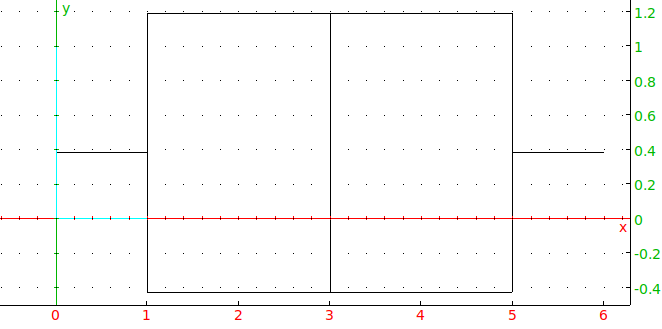
\includegraphics[width=0.75\textwidth]{xcas-whiskerlist.png}
\end{center}
\end{itemize}

\smallskip

\noindent
\textbf{Example.}\\
Define the list \texttt{A} by:\\
\textit{Input:}
\begin{center}
\texttt{A:=[0,1,2,3,4,5,6,7,8,9,10,11]:;}
\end{center}
Then:\\
\textit{Input:}
\begin{center}
  \texttt{mean(A)}
\end{center}
\textit{Output:}
\[
\frac{11}{2}
\]
\textit{Input:}
\begin{center}
  \texttt{stddev(A)}
\end{center}
\textit{Output:}
\[
\frac{2}{12} \sqrt{429}
\]
\textit{Input:}
\begin{center}
  \texttt{quantile(A,0.1)}
\end{center}
\textit{Output:}
\[
1.0
\]
\textit{Input:}
\begin{center}
  \texttt{quantile(A,0.25)}
\end{center}
\textit{Output:}
\[
2.0
\]
\textit{Input:}
\begin{center}
  \texttt{median(A)}
\end{center}
\textit{or:}
\begin{center}
  \texttt{quantile(A,0.5)}
\end{center}
\textit{Output:}
\[
5.0
\]
\textit{Input:}
\begin{center}
  \texttt{quantile(A,0.75)}
\end{center}
\textit{Output:}
\[
8.0
\]
\textit{Input:}
\begin{center}
  \texttt{quantile(A,0.9)}
\end{center}
\textit{Output:}
\[
10.0
\]
\textit{Input:}
\begin{center}
  \texttt{max(A)}
\end{center}
\textit{Output:}
\[
11
\]
\textit{Input:}
\begin{center}
  \texttt{quartiles(A)}
\end{center}
\textit{Output:}
\[
\left[\begin{array}{c}0.0\\2.0\\5.0\\8.0\\11.0\end{array}\right]
\]

\section{Tables with strings as indices: \texttt{table}
\index{table}
\label{sec:table}}

A table is a map (associative container) used to store
information associated to indices which are much more general than
integers, such as  strings or sequences. For example, you can use one to
store a table of phone numbers indexed by names.

In \texttt{Xcas}, the indices in a table may be any kind of \texttt{Xcas} objects.
Access is done by a binary search algorithm, where the sorting
function first sorts by \texttt{type} then uses an order for each type
(e.g. $<$ for numeric types, lexicographic order for strings, etc.)

The \texttt{table} command creates a table.
\begin{itemize}
  \item \texttt{table} takes an unspecified number of arguments:\\
   \textit{seq}, a list or sequence of equalities
  of the form \textit{index\_name}\texttt{=}\textit{element\_value}.
  \item \texttt{table(}\textit{seq}\texttt{)} returns a table.  The
  elements of the table can be retrieved using index bracket notation;
  If $T$ is the name of the table, then $T$(\textit{index\_name})
  returns \textit{element\_value}.
\end{itemize}

\smallskip

\noindent
\textbf{Example.}\\
\textit{Input:}
\begin{center}
\texttt{T:=table(3=-10,"a"=10,"b"=20,"c"=30,"d"=40):;}
\end{center}
\textit{Input:}
\begin{center}
\texttt{T["b"]}
\end{center}
\textit{Output:}
\[
20
\]
%\begin{center}\texttt{20}\end{center}
\textit{Input:}
\begin{center}
\texttt{T[3]}
\end{center}
\textit{Output:}
\[
-10
\]
%\begin{center}\texttt{-10}\end{center}

\smallskip

\noindent 
\textbf{Remark.}\\ 
Tables can be created and the elements of a table can be changed using
the \texttt{:=} assignment.
\begin{itemize}
  \item If \texttt{T} is a symbolic variable then the assignment
  \texttt{T(}\textit{index\_name}\texttt{:=}\textit{element\_value}
  will create a table \texttt{T} with one element.
  \item If $n$ is an integer, then the assignment
  \texttt{T($n$):=}\textit{obj} will do the following:
  \begin{itemize}
  \item If the variable \texttt{T} was assigned to a list or a sequence,
  then the $n$th element of \texttt{T} is modified.
  \item if the variable \texttt{T} was not assigned, a table \texttt{T}
  is created with one entry (corresponding to the index $n$). Note
  that after the assignment \texttt{T} is not a list, despite the fact that $n$
  is an integer.
  \end{itemize}
\end{itemize}

\section{Matrices\label{sec:defmat}}

\subsection{Matrices}

A matrix is represented by a list of lists, all having the same size.

\smallskip

\noindent
\textbf{Example.}\\
\textit{Input:}
\begin{center}
  \texttt{[[1,2,3],[4,5,6]]}
\end{center}
\textit{Output:}
\[
\left[\begin{array}{ccc}1&2&3\\4&5&6\end{array}\right]
\]

\smallskip

You can give a matrix a name with assignment.\\
\textit{Input:}
\begin{center}
  \texttt{A:= [[1,2,6], [3,4,8], [1,0,1]]}
\end{center}
\textit{Output:}
\[
\left[\begin{array}{ccc}1&2&6\\3&4&8\\1&0&1\end{array}\right]
\]

\subsection{Special matrices}

\subsubsection{Identity matrix: \texttt{idn} \texttt{identity}
\index{idn}
\index{identity}}

The \texttt{idn} command finds identity matrices.
\begin{itemize}
  \item \texttt{idn} takes one argument:\\
  $n$, a positive integer or\\
  $A$, a square matrix.
  \item \texttt{idn($n$)} returns the $n\times n$ identity matrix.
  \item \texttt{idn($A$)} returns the identity matrix the same size as
  $A$.
\end{itemize}

\smallskip

\noindent
\textbf{Examples.}
\begin{itemize}
\item 
\textit{Input:}
\begin{center}
\texttt{idn(3)}
\end{center}
\textit{Output:}
\[
\begin{pmatrix}1&0&0\\0&1&0\\0&0&1\end{pmatrix}
\]
\item
\textit{Input:}
\begin{center}
  \texttt{idn([[2,3],[4,5]]}
\end{center}
\texttt{Output:}
\[
\begin{pmatrix}1&0\\0&1\end{pmatrix}
\]
\end{itemize}

\subsubsection{Zero matrix: \texttt{newMat}
\index{newMat}}

The \texttt{newMat} command creates a matrix of all 0s.
\begin{itemize}
  \item \texttt{newMat} takes two arguments:\\
  $n$ and $p$, two positive integers.
  \texttt{newMat($n,p$)} returns the $n\times p$ zero matrix.
\end{itemize}

\smallskip

\noindent
\textbf{Example.}\\
\textit{Input:}
\begin{center}
\texttt{newMat(4,4)}
\end{center}
\textit{Output:}
\[
\left[\begin{array}{cccc}0&0&0&0\\0&0&0&0\\0&0&0&0\\0&0&0&0\end{array}\right]
\]

% \subsection{Random matrix: \texttt{ranm} \texttt{randMat} \texttt{randmatrix}\label{ssec:ranm2}}
% \index{ranm}
% \index{randMat}
% \index{randmatrix}

% \noindent\texttt{ranm} or \texttt{randMat} or \texttt{randmatrix}
% takes as argument an integer $n$ or two integers $n,m$ and optionally
% a third argument, either an integer $k$ or the quoted name of a random
% distribution law
% (see also \ref{ssec:ranm1} and  \ref{ssec:randvector}.\\ % and \ref{ssec:ranm3}).\\
% \texttt{ranm} returns a vector of size $n$ or a matrix of size $n\times m$
%  containing random integers uniformly distributed between -99 and +99
% (default), or between 0 and $k-1$ or  a matrix  of size $n\times m$
% containing random integers according to the law put between quotes.\\
% Input:
% \begin{center}\texttt{ranm(3)}\end{center}
% Output:
% \begin{center}\texttt{[-54,78,-29]}\end{center}
% Input:
% \begin{center}\texttt{ranm(2,4)}\end{center}
% Output:
% \begin{center}\texttt{[[27,-29,37,-66],[-11,76,65,-33]]}\end{center}
% Input:
% \begin{center}\texttt{ranm(2,4,3)}\end{center}
% or:
% \begin{center}\texttt{ranm(2,4,'rand(3)')}\end{center}
% Output:
% \begin{center}\texttt{[[0,1,1,0],[0,1,2,0]]}\end{center}
% Input:
% \begin{center}\texttt{ranm(2,4,'randnorm(0,1)')}\end{center}
% Output:
% \begin{center}\texttt{[[1.83785427742,0.793007112053,-0.978388964902,-1.88602023857], [-1.50900874199,-0.241173369698,0.311373795585,-0.532752431454]]}\end{center}
% Input:
% \begin{center}\texttt{ranm(2,4,2..4)}\end{center}
% Output:
% \begin{center}\texttt{[[2.00549363438,3.03381264955,2.06539073586,2.04844321217],
%  [3.88383254968,3.28664474655,3.76909781061,2.39113253355]]}\end{center}


\subsubsection{Diagonals of matrices and diagonal matrices: \texttt{BlockDiagonal} \texttt{diag}
\index{diag}
\index{BlockDiagonal}
\label{ssec:diag}}

The \texttt{diag} command either creates a diagonal matrix or finds
the diagonal elements of an existing matrix.\\
\texttt{BlockDiagonal} is a synonym for \texttt{diag}.
\begin{itemize}
  \item \texttt{diag} takes one argument:\\
  $L$, a list or a square matrix.
  \item \texttt{diag($L$)} (for a list $L$) returns the diagonal
  matrix with the entries of $L$ on the diagonal.
  \item  \texttt{diag($L$)} (for a matrix $L$) returns a list
  consisting of the diagonal elements of $L$.
\end{itemize}

\smallskip

\noindent
\textbf{Examples.}
\begin{itemize}
\item 
\textit{Input:}
\begin{center}
\texttt{diag([1,4])}
\end{center}
\textit{Output:}
\[
\left[\begin{array}{cc}1&0\\0&4\end{array}\right]
\]
\item
\textit{Input:}
\begin{center}
\texttt{diag([[1,2],[3,4]])}
\end{center}
\textit{Output:}
\[
\left[1,4\right]
\]
\end{itemize}

\subsubsection{Jordan block: \texttt{JordanBlock}
\index{JordanBlock}}

The \texttt{JordanBlock} command creates a Jordan Block; i.e., a
square matrix with the same value for all diagonal elements, 1s just
above the diagonal, and 0s everyone else.
\begin{itemize}
  \item \texttt{JordanBlock} takes two arguments:
  \begin{itemize}
    \item $a$, an expression.
    \item $n$, a positive integer.
  \end{itemize}
  \texttt{JordanBlock($a,n$)} returns the $n\times n$ matrix
  with $a$s on the principal diagonal, 1s above this diagonal and 0s  
  everywhere else.
\end{itemize}

\smallskip

\noindent
\textbf{Example.}\\
\textit{Input:}
\begin{center}
\texttt{JordanBlock(7,3)}
\end{center}
\textit{Output:}
\[
\left[\begin{array}{ccc}7&1&0\\0&7&1\\0&0&7\end{array}\right]
\]

\subsubsection{Hilbert matrix: \texttt{hilbert}
\index{hilbert}}

A Hilbert matrix is a square matrix whose element in the $i$th row and
$j$th column (recall the numbering starting at 0) is
\[
a_{j,k}=\frac{1}{j+k+1}
\]
The \texttt{hilbert} command finds Hilbert matrices.
\begin{itemize}
  \item \texttt{hilbert} takes one argument:\\
  $n$, a positive integer.
  \item \texttt{hilbert($n$)} returns the $n\times n$ Hilbert matrix.
\end{itemize}

\smallskip

\noindent
\textbf{Example.}\\
\textit{Input:}
\begin{center}
\texttt{hilbert(4)}
\end{center}
\textit{Output:}
\[
\begin{pmatrix}1&\frac{1}{2}&\frac{1}{3}&\frac{1}{4}\\\frac{1}{2}&\frac{1}{3}&\frac{1}{4}&\frac{1}{5}\\\frac{1}{3}&\frac{1}{4}&\frac{1}{5}&\frac{1}{6}\\\frac{1}{4}&\frac{1}{5}&\frac{1}{6}&\frac{1}{7}\end{pmatrix}
\]

\subsubsection{Vandermonde matrix: \texttt{vandermonde}
\index{vandermonde}}

A Vandermonde matrix is a square matrix where each row starts with a 1
and is in geometric progression.  The \texttt{vandermonde} command
finds a Vandermonde matrix.
\begin{itemize}
  \item \texttt{vandermonde} takes one argument:\\
  $X=[x_{0},\ldots,x_{n-1}]$, a vector.
  \item \texttt{vandermonde($X$)} returns the corresponding
  Vandermonde matrix; namely, the $k$-th row of the
  matrix is the vector whose components are $x_i^{k}$ for $i=0..n-1$ and
  $k=0..n-1$.
\end{itemize}

\smallskip

\noindent
\textbf{Warning!}\\ 
The indices of the rows and columns begin at 0 with \texttt{Xcas}.

\smallskip

\noindent
\textbf{Example.}\\
\textit{Input:}
\begin{center}
\texttt{vandermonde([a,2,3])}
\end{center}
\textit{Output (if \texttt{a} is symbolic else purge(a)):}
\[
\begin{pmatrix}1&a&a a\\1&2&4\\1&3&9\end{pmatrix}
\]

\subsection{Combining matrices}

\subsubsection{Making a matrix with a list of matrices: \texttt{blockmatrix}
\index{blockmatrix}}

The \texttt{blockmatrix} combines several matrices into one larger
matrix.
\begin{itemize}
\item \texttt{blockmatrix} takes three arguments:
\begin{itemize}
  \item $m$ and $n$, two positive integers.
  \item $L$, a list of $m\cdot n$ matrices such that the first $m$
  matrices have the same number of rows; the next $m$ matrices have
  the same number of rows, etc; and the number of columns in each
  group of $m$ matrices is the same (for example, all the matrices in
  $L$ could have the same dimension), so that the $n$ groups of $m$
  matrices can be stacked above each other to form a larger matrix.
  \end{itemize}
  \item \texttt{blockmatrix($m,n,L$)} returns the larger matrix formed
  by the matrices in $L$ by putting each group of $m$ matrices next to
  each other, and stacking the resulting $n$ matrices on top of each
  other.
  
  If the matrices in $L$ each have the same dimension $p \times q$,
  the result will be a matrix with dimension $p*n \times q*m$.
\end{itemize}

\smallskip

\noindent
\textbf{Examples.}
\begin{itemize}
\item 
\textit{Input:}
\begin{center}
\texttt{blockmatrix(2,3,[idn(2),idn(2),idn(2), idn(2),idn(2),idn(2)])}
\end{center}
\textit{Output:}
\[
\left[\begin{array}{cccccc}1&0&1&0&1&0\\0&1&0&1&0&1\\1&0&1&0&1&0\\0&1&0&1&0&1\end{array}\right]
\]
%\begin{center}\texttt{[[1,0,1,0,1,0],[0,1,0,1,0,1], [1,0,1,0,1,0],[0,1,0,1,0,1]]}\end{center}
\item
\textit{Input:}
\begin{center}
\texttt{blockmatrix(3,2,[idn(2),idn(2), idn(2),idn(2),idn(2),idn(2)])}
\end{center}
\textit{Output:}
\[
\left[\begin{array}{cccc}1&0&1&0\\0&1&0&1\\1&0&1&0\\0&1&0&1\\1&0&1&0\\0&1&0&1\end{array}\right]
\]
%\begin{center}\texttt{[[1,0,1,0],[0,1,0,1], [1,0,1,0],[0,1,0,1],[1,0,1,0],[0,1,0,1]]}\end{center}
\item
\textit{Input:}
\begin{center}
\texttt{blockmatrix(2,2,[idn(2),newMat(2,3), newMat(3,2),idn(3)])}
\end{center}
\textit{Output:}
\[
\left[\begin{array}{ccccc}1&0&0&0&0\\0&1&0&0&0\\0&0&1&0&0\\0&0&0&1&0\\0&0&0&0&1\end{array}\right]
\]
%\begin{center}\texttt{[[1,0,0,0,0],[0,1,0,0,0],[0,0,1,0,0], [0,0,0,1,0],[0,0,0,0,1]]}\end{center}
\item
\textit{Input:}
\begin{center}
\texttt{blockmatrix(3,2,[idn(1),newMat(1,4), newMat(2,3),idn(2),newMat(1,2),[[1,1,1]]])}
\end{center}
\textit{Output:}
\[
\left[\begin{array}{ccccc}1&0&0&0&0\\0&0&0&1&0\\0&0&0&0&1\\0&0&1&1&1\end{array}\right]
\]
%\begin{center}\texttt{[[1,0,0,0,0],[0,0,0,1,0],[0,0,0,0,1],[0,0,1,1,1]]}\end{center}
\textit{Input:}
\begin{center}
\begin{tabular}{l}
  \texttt{A:=[[1,1],[1,1]];B:=[[1],[1]]:;}\\
  \texttt{blockmatrix(2,3,[2*A,3*A,4*A,5*B,newMat(2,4),6*B])}
\end{tabular}
\end{center}
\textit{Output:}
\[
\left[\begin{array}{cccccc}2&2&3&3&4&4\\2&2&3&3&4&4\\5&0&0&0&0&6\\5&0&0&0&0&6\end{array}\right]
\]
%\begin{center}\texttt{[[2,2,3,3,4,4],[2,2,3,3,4,4], [5,0,0,0,0,6],[5,0,0,0,0,6]]}\end{center}
\end{itemize}

\subsubsection{Making a matrix from two matrices: \texttt{semi\_augment}
\index{semi\_augment|textbf}}

The \texttt{semi\_augment} command concatenates two matrices with the
same number of columns.
\begin{itemize}
  \item \texttt{semi\_augment} takes two arguments:\\
  $A$ and $B$, two matrices with the same number of columns.
  \item \texttt{semi\_augment($A,B$)} returns the matrix which has the
  rows of $A$ followed by the rows of $B$.
\end{itemize}

\smallskip

\noindent
\textbf{Examples.}
\begin{itemize}
\item 
\textit{Input:}
\begin{center}
\texttt{semi\_augment([[3,4],[2,1],[0,1]],[[1,2],[4,5]])}
\end{center}
\textit{Output:}
\[
\left[\begin{array}{cc}3&4\\2&1\\0&1\\1&2\\4&5\end{array}\right]
\]
\begin{center}\texttt{[[3,4],[2,1],[0,1],[1,2],[4,5]]}\end{center}
\item
\textit{Input:}
\begin{center}
\texttt{semi\_augment([[3,4,2]],[[1,2,4]])}
\end{center}
\textit{Output:}
\[
\left[\begin{array}{ccc}3&4&2\\1&2&4\end{array}\right]
\]
%\begin{center}\texttt{[[3,4,2],[1,2,4]]}\end{center}
Note the difference with \texttt{concat}.\\
\textit{Input:}
\begin{center}
\texttt{concat([[3,4,2]],[[1,2,4]]}
\end{center}
\textit{Output:}
\[
\left[\begin{array}{cccccc}3&4&2&1&2&4\end{array}\right]
\]
%\begin{center}\texttt{[[3,4,2,1,2,4]]}\end{center}
Indeed, when the two matrices $A$ and  $B$ have the same dimension, \texttt{concat}
makes a matrix with the same number of rows as $A$ and $B$ by
gluing them side by side.\\
\textit{Input:}
\begin{center}
\texttt{concat([[3,4],[2,1],[0,1]],[[1,2],[4,5]]}
\end{center}
\textit{Output:}
\[
\left[\begin{array}{cc}3&4\\2&1\\0&1\\1&2\\4&5\end{array}\right]
\]
%\begin{center}\texttt{[[3,4],[2,1],[0,1],[1,2],[4,5]]}\end{center}
\textit{but input:}
\begin{center}
\texttt{concat([[3,4],[2,1]],[[1,2],[4,5]]}
\end{center}
\textit{Output:}
\[
\left[\begin{array}{cccc}3&4&1&2\\2&1&4&5\end{array}\right]
\]
% \begin{center}
% \texttt{[[3,4,1,2],[2,1,4,5]]}
% \end{center}
\end{itemize}

\subsubsection{Making a  matrix from two matrices: \texttt{augment} \texttt{concat}
\index{augment}
\index{concat}}

The \texttt{augment} command glues two matrices, either side by side
or one on top of the other.\\
Here, \texttt{concat} can be used as a synonym for \texttt{augment}.
\begin{itemize}
  \item \texttt{augment} has two arguments:\\
  $A$ and $B$, two matrices with the same number of rows or the same
  number of columns.
  \item \texttt{augment($A,B$)} returns the matrix consisting of:
  \begin{itemize}
    \item if $A$ and $B$ have the same number of rows, then the matrix
    being returned consists of the columns of $A$ followed by the
    columns of $B$; in other words, $A$ and $B$ are glued side by side.
    \item if $A$ and $B$ do not have the same number of rows but have
    the same number of columns, then the matrix being returned
    consists of the rows of $A$ followed by the rows of $B$; in other
    words, $A$ and $B$ are glued one on top of the other.
  \end{itemize}
\end{itemize}

\smallskip

\noindent
\textbf{Examples.}
\begin{itemize}
\item 
\textit{Input:}
\begin{center}
\texttt{augment([[3,4,5],[2,1,0]],[[1,2],[4,5]])}
\end{center}
\textit{Output:}
\[
\left[\begin{array}{ccccc}3&4&5&1&2\\2&1&0&4&5\end{array}\right]
\]
%\begin{center}\texttt{[[3,4,5,1,2],[2,1,0,4,5]]}\end{center}
\item
\textit{Input:}
\begin{center}
\texttt{augment([[3,4],[2,1],[0,1]],[[1,2],[4,5]])}
\end{center}
\textit{Output:}
\[
\left[\begin{array}{cc}3&4\\2&1\\0&1\\1&2\\4&5\end{array}\right]
\]
%\begin{center}\texttt{[[3,4],[2,1],[0,1],[1,2],[4,5]]}\end{center}
\item
\textit{Input:}
\begin{center}
\texttt{augment([[3,4,2]],[[1,2,4]]}
\end{center}
\textit{Output:}
\[
\left[\begin{array}{cccccc}3&4&2&1&2&4\end{array}\right]
\]
%\begin{center}\texttt{[[3,4,2,1,2,4]]}\end{center}
\end{itemize}

Note that if $A$ and $B$ have the same dimension, then
\texttt{augment($A,B$)} will return a matrix with the same number of
rows as $A$ and $B$ by horizontal gluing.  In that case, if you want
to combine them by vertical gluing, you must use
\texttt{semi\_augment($A,B$)}.
% Input:
% \begin{center}\texttt{augment([[3,4],[2,1]],[[1,2],[4,5]])}\end{center}
% Output:
% \begin{center}\texttt{[[3,4,1,2],[2,1,4,5]]]}\end{center}

\subsubsection{Appending a column to a matrix: \texttt{border}
\index{border}}

The \texttt{border} command adds a column to a matrix.
\begin{itemize}
  \item \texttt{border} takes two arguments:
  \begin{itemize}
    \item $A$, a matrix.
    \item $b$, a list whose length equals the number of rows of $A$.
  \end{itemize}
  \item \texttt{border($A,L$)} returns a matrix equal to $A$ with the
  transpose of $L$ forming an additional column to the right; so
  \begin{center}
    \texttt{border($A,b$)=tran([op(tran($A$)),$b$])=tran(append(tran($A$),$b$))}    
  \end{center}
\end{itemize}

\smallskip

\noindent
\textbf{Examples.}
\begin{itemize}
\item 
\textit{Input:}
\begin{center}
\texttt{border([[1,2,4],[3,4,5]],[6,7])}
\end{center}
\textit{Output:}
\[
\left[\begin{array}{cccc}1&2&4&6\\3&4&5&7\end{array}\right]
\]
%\begin{center}\texttt{[[1,2,4,6],[3,4,5,7]]}\end{center}
\item
\textit{Input:}
\begin{center}
\texttt{border([[1,2,3,4],[4,5,6,8],[7,8,9,10]],[1,3,5])}
\end{center}
\textit{Output:}
\[
\left[\begin{array}{ccccc}1&2&3&4&1\\4&5&6&8&3\\7&8&9&10&5\end{array}\right]
\]
%\begin{center}\texttt{[[1,2,3,4,1],[4,5,6,8,3],[7,8,9,10,5]]}\end{center}
\end{itemize}

\subsection{Creating a matrix with a formula or function: \texttt{makemat} \texttt{matrix}
\index{makemat}
\index{matrix}
\label{ssec:matrixcommand}}

You can use a function or a formula to specify the elements of a
matrix with the \texttt{makemat} or \texttt{matrix} command.

\begin{itemize}
  \item \texttt{makemat} takes three arguments:
  \begin{itemize}
  \item  $f$, a function of two variables \texttt{j} and
    \texttt{k} which returns the value of $a_{j,k}$, the element at
    row index \texttt{j} and column index \texttt{k} of the resulting
    matrix.
  \item $n$ and $p$, two positive integers.
  \end{itemize}
  \item \texttt{makemat($f,n,p$)} returns the $n\times p$ matrix
    $A=(a_{j,k})$ with $a_{j,k}=f(j,k)$ for $j=1..n$ and $k=1..p$.
\end{itemize}

\smallskip

\noindent
\textbf{Example.}\\
\textit{Input:}
\begin{center}
\texttt{makemat((j,k)->j+k,4,3)}
\end{center}
\textit{or:}
\begin{center}
\begin{tabular}{l}
  \texttt{h(j,k):=j+k}\\
  \texttt{makemat(h,4,3)}
\end{tabular}
\end{center}
\textit{Output:}
\[
\begin{pmatrix}0&1&2\\1&2&3\\2&3&4\\3&4&5\end{pmatrix}
\]
Note that the indices are counted starting from 0.

The \texttt{matrix} command can be used similarly, but note that the
arguments are given in a different order and the indices start at 1.\\
(\texttt{matrix} can also be used to turn tables into matrices; see
\secref{ssec:spmatrices}.)
\begin{itemize}
  \item \texttt{matrix} takes two mandatory arguments and one optional
  argument:
  \begin{itemize}
  \item  $n$ and $p$, two integers.
  \item  Optionally, $f$, a function of two variables \texttt{j} and
  \texttt{k} which should return the value of $a_{j,k}$, the element at
  row index \texttt{j} and column index \texttt{k} of the resulting
  matrix.
  \end{itemize}
  \item \texttt{matrix($n,p$)} returns the $n\times p$ matrix consisting of
    all 0s.
  \item \texttt{matrix($n,p,f$)} returns the $n\times p$ matrix
    $A=(a_{j,k})$ with $a_{j,k}=f(j,k)$ for $j=1..n$ and $k=1..p$.
\end{itemize}

\smallskip

\noindent
\textbf{Examples.}
\begin{itemize}
\item
\textit{Input:}
\begin{center}
  \texttt{matrix(2,3)}
\end{center}
\textit{Output:}
\[
\begin{pmatrix}0&0&0\\0&0&0\end{pmatrix}
\]
\item 
\textit{Input:}
\begin{center}
\texttt{matrix(4,3,(j,k)->j+k)}
\end{center}
\textit{or:}
\begin{center}
\begin{tabular}{l}
  \texttt{h(j,k):=j+k}\\
  \texttt{matrix(4,3,h)}
\end{tabular}
\end{center}
\textit{Output:}
\[
\begin{pmatrix}0&1&2\\1&2&3\\2&3&4\\3&4&5\end{pmatrix}
\]
%\begin{center}\texttt{[[2,3,4],[3,4,5],[4,5,6],[5,6,7]]}\end{center}
\end{itemize}

%In the \texttt{Xcas} answers, the matrix delimiters are \textbf{[]}
%(bold brackets). For example, \textbf{[}1,2,3\textbf{]} is the matrix
%[[1,2,3]] with only one row, unlike [1,2,3] (normal brackets) which is
%the list [1,2,3].\\ In this document, the input notation ([[1,2,3]])
%will be used for input and output.

\subsection{Getting the parts of a matrix}

\subsubsection{Accessing parts of a matrix: \texttt{[]} \texttt{at}
\index{at}}

The rows of a matrix are the elements of a list, and can be accessed
with indices using the postfix \texttt{[\ldots]} or the prefix
\texttt{at} (see \secref{ssec:getels}).

\smallskip

\noindent
\textbf{Example.}\\ 
\textit{Input:}
\begin{center}
  \texttt{A:= [[1,2,6], [3,4,8], [1,0,1]]}
\end{center}
\textit{then:}
\begin{center}
  \texttt{A[0]}
\end{center}
\textit{or:}
\begin{center}
  \texttt{at(A,0)}
\end{center}
\textit{Output:}
\[
\left[1,2,6\right]
\]

\smallskip

To extract a column of a matrix, you can first turn the columns into
rows with \texttt{transpose} (see \secref{ssec:transpose}), then
extract the row as above.\\

\smallskip

\noindent
\textbf{Example.}\\
\textit{Input:}
\begin{center}
\texttt{tran(A)[1]}
\end{center}
\textit{or:}
\begin{center}
\texttt{at(tran(A),1)}
\end{center}
\textit{Output:}
\[
\left[2,4,0\right]
\]

\smallskip

Individual elements are simply elements of the rows.

\smallskip

\noindent
\textbf{Example.}\\
\textit{Input:}
\begin{center}
  \texttt{A[0][1]}
\end{center}
\textit{Output:}
\[
2
\]
This can be abbreviated by listing the row and column separated by a
comma.\\
\textit{Input:}
\begin{center}
  \texttt{A[0,1]}
\end{center}
\textit{or:}
\begin{center}
  \texttt{at(A,[0,1])}
\end{center}
\textit{Output:}
\[
2
\]
The indexing begins with 0; you can have the indices start with 1
by enclosing them in double brackets.\\
\textit{Input:}
\begin{center}
  \texttt{A[[1,2]]}
\end{center}
\textit{Output:}
\[
2
\]

\smallskip

You can use a range (see \secref{ssec:range}) of indices to get submatrices.

\smallskip

\noindent
\textbf{Examples.}
\begin{itemize}
\item 
\textit{Input:}
\begin{center}
\texttt{A[1,0..2]}
\end{center}
\textit{Output:}
\[
\left[3,4,8\right]
\]
% \begin{center}
% \texttt{[1,2,6]}
% \end{center}
\item
\textit{Input:}
\begin{center}
  \texttt{A[0..2,1]}
\end{center}
\textit{Output:}
\[
\left[2,4,0\right]
\]
\item
\textit{Input:}
\begin{center}
  \texttt{A[0..2,1..2]}
\end{center}
\textit{Output:}
\[
\left[\begin{array}{cc}2&6\\4&8\\0&1\end{array}\right]
\]
\item
\textit{Input:}
\begin{center}
  \texttt{A[0..1,1..2]}
\end{center}
\textit{Output:}
\[
\left[\begin{array}{cc}2&6\\4&8\end{array}\right]
\]
\item
This gives you another way to extract a full column, by specifying all the rows
as an index interval.
\begin{center}
  \texttt{A[0..2,1]}
\end{center}
\textit{Output:}
\[
\left[2,4,0\right]
\]
\end{itemize}

\smallskip

Recall that An index of -1 returns the last element of a list, an
index of -2 the second to last element, etc.

\smallskip

\noindent
\textbf{Examples.}
\begin{itemize}
\item 
\textit{Input:}
\begin{center}
  \texttt{A[-1]}
\end{center}
\textit{Output:}
\[
\left[1,0,1\right]
\]
\item
\textit{Input:}
\begin{center}
  \texttt{A[1,-1]}
\end{center}
\textit{Output:}
\[
8
\]
\end{itemize}

\subsubsection{Extracting rows or columns of a matrix (Maple compatibility): \texttt{row} \texttt{col}
\index{row}
\index{col}}

The \texttt{row} (respectively \texttt{col}) command extracts one or several
rows (respectively columns) of a matrix.

\begin{itemize}
  \item \texttt{row} takes two arguments:
  \begin{itemize}
    \item $A$, a matrix.
    \item $r$, a row index or a range $n_{1}..n_{2}$.
  \end{itemize}
  \item \texttt{row($A,r$)} returns the row or sequence of rows given
  by $r$.
\end{itemize}

\smallskip

\noindent
\textbf{Examples.}
\begin{itemize}
\item 
\textit{Input:}
\begin{center}
\texttt{row([[1,2,3],[4,5,6],[7,8,9]],1)}
\end{center}
\textit{Output:}
\[
\left[4,5,6\right]
\]
\item
\textit{Input:}
\begin{center}
\texttt{row([[1,2,3],[4,5,6],[7,8,9]],0..1)}
\end{center}
\textit{Output:}
\[
\left[1,2,3\right],\left[4,5,6\right]
\]
\end{itemize}

\smallskip

\begin{itemize}
  \item \texttt{col} takes two arguments:
  \begin{itemize}
    \item $A$, a matrix.
    \item $c$, a column index or a range $n_{1}..n_{2}$.
  \end{itemize}
  \item \texttt{row($A,c$)} returns the column or sequence of columns given
  by $c$.
\end{itemize}

\smallskip

\noindent
\textbf{Examples.}
\begin{itemize}
\item 
\textit{Input:}
\begin{center}
\texttt{col([[1,2,3],[4,5,6],[7,8,9]],1)}
\end{center}
\textit{Output:}
\[
\left[2,5,8\right]
\]
\item
\textit{Input:}
\begin{center}
\texttt{col([[1,2,3],[4,5,6],[7,8,9]],0..1)}
\end{center}
\textit{Output:}
\[
\left[1,4,7\right],\left[2,5,8\right]
\]
\end{itemize}

\subsubsection{Extracting a sub-matrix of a matrix (TI compatibility): \texttt{subMat}
\index{subMat}}

The \texttt{subMat} command finds submatrices of a matrix.
\begin{itemize}
  \item \texttt{subMat} takes one mandatory argument and four optional arguments:
  \begin{itemize}
    \item $A$, a matrix.
    \item Optionally, $r_{1}$, an integer, the row index for the
    beginning of the submatrix (by default, $r_{1}=0$).
    \item Optionally, $c_{1}$, an integer, the column index for the
    beginning of the submatrix (by default, $c_{1}=0$).
    \item Optionally, $r_{2}$, an integer, the row index for the
    end of the submatrix (by default, $r_{2}$ equals one less than the
    number of rows of $A$).
    \item Optionally, $c_{2}$, an integer, the column index for the
    end of the submatrix (by default, $c_{1}$ equals one less than the
    number of columns of $A$).
  \end{itemize}
  \item \texttt{subMat($A\,\langle,r_{1},c_{1},r_{2},c_{2}\rangle$)}
  returns the sub-matrix of $A$ from position $(r_{1},c_{1})$ to $(r_{2},c_{2})$.
\end{itemize}

\smallskip

\noindent
\textbf{Example.}\\
\textit{Input:}
\begin{center}
\texttt{A:=[[3,4,5],[1,2,6]]}
\end{center}
\textit{Output:}
\[
\left[\begin{array}{ccc}3&4&5\\1&2&6\end{array}\right]
\]
\begin{itemize}
\item 
\textit{Input:}
\begin{center}
\texttt{subMat(A,0,1,1,2)}
\end{center}
\textit{Output:}
\[
\left[\begin{array}{cc}4&5\\2&6\end{array}\right]
\]
%\begin{center}\texttt{[[4,5],[2,6]]}\end{center}
\item
\textit{Input:}
\begin{center}
\texttt{subMat(A,0,1,1,1)}
\end{center}
\textit{Output:}
\[
\left[\begin{array}{c}4\\2\end{array}\right]
\]
\begin{center}\texttt{[[4],[2]]}\end{center}
\item
\textit{Input:}
\begin{center}
\texttt{subMat(A,1)}
\end{center}
\textit{or:}
\begin{center}
\texttt{subMat(A,1,0)}
\end{center}
\textit{or:}
\begin{center}
\texttt{subMat(A,1,0,1)}
\end{center}
\textit{or:}
\begin{center}
\texttt{subMat(A,1,0,1,2)}
\end{center}
\textit{Output:}
\[
\left[\begin{array}{ccc}1&2&6\end{array}\right]
\]
\end{itemize}

\subsection{Modifying matrices}

\subsubsection{Modifying matrix elements by assignment: \texttt{:=}
\index{:=}}

You can change the elements of a named matrix by assignment
(see \secref{ssec:assign}).

\smallskip

\noindent
\textbf{Example.}\\
\textit{Input:}
\begin{center}
  \texttt{A:= [[1,2,6], [3,4,8], [1,0,1]]}
\end{center}
\textit{then:}
\begin{center}
\begin{tabular}{l}
  \texttt{A[0,1]:= 5:;}\\
  \texttt{A}
\end{tabular}
\end{center}
\textit{Output:}
\[
\left[\begin{array}{ccc}1&5&6\\3&4&8\\1&0&1\end{array}\right]
\]
Recall that the elements are indexed starting at 0, using double
brackets allows you to use indices starting at 1.\\
\textit{Input:}
\begin{center}
\begin{tabular}{l}
  \texttt{A[[1,2]]:=7:;}\\
  \texttt{A}  
\end{tabular}  
\end{center}
\textit{Output:}
\[
\left[\begin{array}{ccc}1&7&6\\3&4&8\\1&0&1\end{array}\right]
\]

\smallskip

You can use assignment to change several entries of a matrix at one.

\smallskip

\noindent
\textbf{Example.}\\
Create a diagonal matrix with a diagonal of \texttt{[1,2,3]}:\\ 
\textit{Input:}
\begin{center}
  \texttt{M:= matrix(3,3)}
\end{center}
\textit{Output:}
\[
\begin{pmatrix}0&0&0\\0&0&0\\0&0&0\end{pmatrix}
\]
\textit{Input:}
\begin{center}
  \texttt{M[0..2,0..2]:= [1,2,3]}
\end{center}
\textit{Output:}
\[
\begin{pmatrix}1&0&0\\0&2&0\\0&0&3\end{pmatrix}
\]
To make the last column \texttt{[4,5,6]}:\\
\textit{Input:}
\begin{center}
  \texttt{M[0..2,2]:= [4,5,6]}
\end{center}
\textit{Output:}
\[
\begin{pmatrix}1&0&4\\0&2&5\\0&0&6\end{pmatrix}
\]

\subsubsection{Modifying matrix elements by reference: \texttt{::=} \texttt{=<}
\index{::=}
\index{=<}}

When you change an element of a matrix with the \texttt{:=}
assignment, a new copy of the matrix is created with the modified
element.  Particularly for large matrices, it is more efficient to use
the \texttt{=<} assignment (see \secref{ssec:refassign}), which will
change the element of the matrix without making a copy.

\smallskip

\noindent
\textbf{Example.}\\
\textit{Input:}
\begin{center}
  \texttt{A:= [[4,5],[2,6]]}
\end{center}
The following commands will all return the matrix \texttt{A} with the
element in the second row, first column, changed to 3.\\
\textit{Input:}
\begin{center}
  \texttt{A[1,0]:= 3}
\end{center}
\textit{or:}
\begin{center}
  \texttt{A[1,0] =< 3}
\end{center}
\textit{or:}
\begin{center}
  \texttt{A[[2,1]]:= 3}
\end{center}
\textit{or:}
\begin{center}
  \texttt{A[[2,1]] =< 3}
\end{center}
\textit{then:}
\begin{center}
  \texttt{A}
\end{center}
\textit{Output:}
\[
\left[\begin{array}{cc}4&5\\3&6\end{array}\right]
\]

You can change larger parts of a matrix simultaneously.

\smallskip

\noindent
\textbf{Example.}\\
\textit{Input:}
\begin{center}
  \texttt{A:= [[4,5],[2,6]]}
\end{center}
The following commands will change
the second row to \texttt{[3,7]}\\
\textit{Input:}
\begin{center}
  \texttt{A[1]:= [3,7]}
\end{center}
\textit{or:}
\begin{center}
  \texttt{A[1] =< [3,7]}
\end{center}
\textit{or:}
\begin{center}
  \texttt{A[[2]]:= [3,7]}
\end{center}
\textit{or:}
\begin{center}
  \texttt{A[[2]] =< [3,7]}
\end{center}
\textit{Output:}
\[
\left[\begin{array}{cc}4&5\\3&7\end{array}\right]
\]

The \texttt{=<} assignment must be used carefully, since it not only
modifies a matrix \texttt{A}, it modifies all objects pointing to
\texttt{A}.  In a program, initialization should contain a line like
\texttt{A:= copy(B)} (see \secref{ssec:copy}) so modifications done on
\texttt{A} don't affect \texttt{B}, and modifications done on
\texttt{B} don't affect \texttt{A}.

For example:\\
\textit{Input:}
\begin{center}
  \texttt{B:= [[4,5],[2,6]]}
\end{center}
\textit{then:}
\begin{center}
  \texttt{A:= B}
\end{center}
\textit{or:}
\begin{center}
  \texttt{A =< B}
\end{center}
creates two matrices equal to
\[
\left[\begin{array}{cc}4&5\\2&6\end{array}\right]
\]
\textit{Input:}
\begin{center}
  \texttt{A[1] =< [3,7]}
\end{center}
\textit{or:}
\begin{center}
  \texttt{B[1] =< [3,7]}
\end{center}
transforms both \texttt{A} and \texttt{B} to 
\[
\left[\begin{array}{cc}4&5\\3&7\end{array}\right]
\]

On the other hand, creating \texttt{A} and \texttt{B} with:\\
\textit{Input:}
\begin{center}
\begin{tabular}{l}
  \texttt{B:= [[4,5],[2,6]]}\\
  \texttt{A:= copy(B)}
\end{tabular}
\end{center}
will again create two matrices equal to
\[
\left[\begin{array}{cc}4&5\\2&6\end{array}\right]
\]
But:\\
\textit{Input:}
\begin{center}
  \texttt{A[1] =< [3,7]}
\end{center}
will change \texttt{A} to 
\[
\left[\begin{array}{cc}4&5\\3&7\end{array}\right]
\]
but \texttt{B} will still be
\[
\left[\begin{array}{cc}4&5\\2&6\end{array}\right]
\]

\subsubsection{Modifying an element or a row of a matrix: \texttt{subsop}
\index{subsop|textbf}}

The \texttt{subsop} command modifies elements of lists (see
\secref{ssec:subsoplist}), and so you can use it to modify elements or rows of matrices.
It is used mainly for \texttt{Maple} and \texttt{MuPAD} compatibility,
and the argument list is in a different order in \texttt{Maple} mode. Unlike
\texttt{:=} or \texttt{=<}, it does not require the matrix to be
stored in a variable.

Let \texttt{A} be the matrix give by:\\
\textit{Input:}
\begin{center}
  \texttt{A:=[[4,5],[2,6]]}
\end{center}

\paragraph{In \texttt{Xcas}, \texttt{Mupad} and \texttt{TI} modes:}

Recall that the indexing in \texttt{Xcas} mode begins with 0, while in
\texttt{Mupad} and \texttt{TI} modes it begins with 1.

To modify an element:
\begin{itemize}
  \item \texttt{subsop} takes two arguments:
  \begin{itemize}
    \item $A$, a matrix.
    \item \texttt{[$r,c$]=$v$}, an equality between a matrix position
    (given as a list) and a value.\\
    The two sides of the equality can also be given as separate
    arguments.
  \end{itemize}
  \texttt{subsop($A$,[$r,c$]=$v$)} returns the matrix which is the
  same as $A$ except that the element in row $r$, column $c$ is now $v$.
\end{itemize}

\smallskip

\noindent
\textbf{Examples.}
\begin{itemize}
\item 
\textit{Input (in \texttt{Xcas} mode):}
\begin{center}
\texttt{subsop([[4,5],[2,6]],[1,0]=3)}
\end{center}
\textit{or:}
\begin{center}
\texttt{subsop([[4,5],[2,6]],[1,0],3)}
\end{center}
\textit{Output:}
\[
\left[\begin{array}{cc}4&5\\3&6\end{array}\right]
\]
\item
\textit{Input (in \texttt{Mupad} or \texttt{TI} mode):}
\begin{center}
\texttt{subsop([[4,5],[2,6]],[2,1]=3)}
\end{center}
\textit{or:}
\begin{center}
\texttt{subsop([[4,5],[2,6]],[2,1],3)}
\end{center}
\textit{Output:}
\[
\left[\begin{array}{cc}4&5\\3&6\end{array}\right]
\]
\end{itemize}

\smallskip

To modify a row:
\begin{itemize}
  \item \texttt{subsop} takes two arguments:
  \begin{itemize}
    \item $A$, a matrix.
    \item $r=L$, an equality between a row index and a list with the
    same length as the rows of $A$.\\
    The two sides of the equality can also be given as separate
    arguments.
  \end{itemize}
  \item \texttt{subsop($A,r=L$)} returns the matrix which is the
  same as $A$ except that row $r$ is now equal to the list $L$.
\end{itemize}

\smallskip

\noindent
\textbf{Examples.}
\begin{itemize}
\item 
\textit{Input (in \texttt{Xcas} mode):}
\begin{center}
\texttt{subsop([[4,5],[2,6]],1=[3,3])}
\end{center}
\textit{or:}
\begin{center}
\texttt{subsop([[4,5],[2,6]],1,[3,3])}
\end{center}
\textit{Output:}
\[
\left[\begin{array}{cc}4&5\\3&3\end{array}\right]
\]
\item
\textit{Input (in \texttt{Mupad} or \texttt{TI} mode):}
\begin{center}
\texttt{subsop([[4,5],[2,6]],2=[3,3])}
\end{center}
\textit{or:}
\begin{center}
\texttt{subsop([[4,5],[2,6]],2,[3,3])}
\end{center}
\textit{Output:}
\[
\left[\begin{array}{cc}4&5\\3&3\end{array}\right]
\]
\end{itemize}

\paragraph{In \texttt{Maple} mode:}

Recall that the indexing in \texttt{Maple} mode
begins with 1.

To modify an element:
\begin{itemize}
  \item \texttt{subsop} takes two arguments:
  \begin{itemize}
    \item \texttt{[$r,c$]=$v$}, an equality between a matrix position
    (given as a list) and a value.\\
    The two sides of the equality can also be given as separate
    arguments.
    \item $A$, a matrix.
  \end{itemize}
  \texttt{subsop([$r,c$]=$v$,$A$)} returns the matrix which is the
  same as $A$ except that the element in row $r$, column $c$ is now $v$.
\end{itemize}

\smallskip

\noindent
\textbf{Example.}\\
\textit{Input:}
\begin{center}
\texttt{subsop([2,1]=3,[[4,5],[2,6]])}
\end{center}
\textit{Output:}
\[
\left[\begin{array}{cc}4&5\\3&6\end{array}\right]
\]

\smallskip

To modify a row:
\begin{itemize}
  \item \texttt{subsop} takes two arguments:
  \begin{itemize}
    \item $r=L$, an equality between a row index and a list with the
      same length as the rows of the second argument $A$.
    \item $A$, a matrix.
  \end{itemize}
  \item \texttt{subsop($r=L,A$)} returns the matrix which is the
  same as $A$ except that row $r$ is now equal to the list $L$.
\end{itemize}

\smallskip

\textbf{Example:}\\
\textit{Input (in \texttt{Maple} mode):}
\begin{center}
\texttt{subsop(2=[3,3],[[4,5],[2,6]])}
\end{center}
\textit{Output:}
\[
\left[\begin{array}{cc}4&5\\3&3\end{array}\right]
\]

\paragraph{In all modes:}

If the matrix is stored in a variable, for example with the matrix
\texttt{A} as above, it is easier to enter \texttt{A[1,0]:=3} and
\texttt{A[1]=[3,3]} to modify \texttt{A} as above.

Also, note that \texttt{subsop} with a \texttt{'n=NULL'} argument
deletes row number \texttt{n}.

\smallskip

\noindent
\textbf{Example.}\\
\textit{Input (in \texttt{Xcas} mode):}
\begin{center}
\texttt{subsop([[4,5],[2,6]],'1=NULL')}
\end{center}
\textit{Output:}
\[
\left[\begin{array}{cc}4&5\end{array}\right]
\]

\subsubsection{Removing rows or columns of a matrix: \texttt{delrows} \texttt{delcols}
\index{delrows}
\index{delcols}}

The \texttt{delrows} (respectively \texttt{delcols}) command removes
one or more rows (respectively columns) from a matrix.

\begin{itemize}
  \item \texttt{delrows} takes two arguments:
  \begin{itemize}
    \item $A$, a matrix.
    \item $r$, an integer or a range of integers.
  \end{itemize}
  \item \texttt{delrows($A,r$)} returns the matrix equal to $A$ with
  the row(s) given by $r$ removed.
\end{itemize}

\smallskip

\noindent
\textbf{Examples.}
\begin{itemize}
\item 
\textit{Input:}
\begin{center}
\texttt{delrows([[1,2,3],[4,5,6],[7,8,9]],1)}
\end{center}
\textit{Output:}
\[
\left[\begin{array}{ccc}1&2&3\\7&8&9\end{array}\right]
\]
\item
\textit{Input:}
\begin{center}
\texttt{delrows([[1,2,3],[4,5,6],[7,8,9]],0..1)}
\end{center}
\textit{Output:}
\[
\left[\begin{array}{ccc}7&8&9\end{array}\right]
\]
\end{itemize}

\smallskip

The \texttt{delcols} command behaves like \texttt{delrows}, but for
columns.
\begin{itemize}
  \item \texttt{delcols} takes two arguments:
  \begin{itemize}
    \item $A$, a matrix.
    \item $c$, an integer or a range of integers.
  \end{itemize}
  \item \texttt{delrows($A,c$)} returns the matrix equal to $A$ with
  the column(s) given by $c$ removed.
\end{itemize}

\smallskip

\noindent
\textbf{Examples.}
\begin{itemize}
\item 
\textit{Input:}
\begin{center}
\texttt{delcols([[1,2,3],[4,5,6],[7,8,9]],1)}
\end{center}
\textit{Output:}
\[
\left[\begin{array}{cc}1&3\\4&6\\7&9\end{array}\right]
\]
\item
\textit{Input:}
\begin{center}
\texttt{delcols([[1,2,3],[4,5,6],[7,8,9]],0..1)}
\end{center}
\textit{Output:}
\[
\left[\begin{array}{c}3\\6\\9\end{array}\right]
\]
\end{itemize}

\subsubsection{Resizing a matrix or vector: \texttt{REDIM} \texttt{redim}
\index{REDIM}
\index{redim}}

The \texttt{REDIM} command resizes matrices and vectors.\\
\texttt{redim} is a synonym for \texttt{REDIM}.

For matrices:
\begin{itemize}
  \item \texttt{REDIM} takes two arguments:
  \begin{itemize}
    \item $A$, a matrix.
    \item \texttt{[$m,n$]}, a list of two positive integers.
  \end{itemize}
  \item \texttt{REDIM($A$,[$m,n$])} returns $A$ resized to an $m\times
  n$ matrix, removing elements (if necessary) to make it smaller and
  adding 0s (if necessary) to make it larger.
\end{itemize}

\smallskip

\noindent
\textbf{Examples.}
\begin{itemize}
\item 
\textit{Input:}
\begin{center}
  \texttt{REDIM([[4,1,-2],[1,2,-1],[2,1,0]],[5,4])}
\end{center}
\textit{Output:}
\[
\begin{pmatrix}4&1&-2&0\\1&2&-1&0\\2&1&0&0\\0&0&0&0\\0&0&0&0\end{pmatrix}
\]
% \begin{center}
%   \tt
%   [[4,1,-2,0],[1,2,-1,0],[2,1,0,0],[0,0,0,0],[0,0,0,0]]
% \end{center}
\item
\textit{Input:}
\begin{center}
  \texttt{REDIM([[4,1,-2],[1,2,-1],[2,1,0]],[2,1])}
\end{center}
\textit{Output:}
\[
\begin{pmatrix}4\\1\end{pmatrix}
\]
% \begin{center}
%   \tt
%    [[4],[1]]
% \end{center}
\end{itemize}

\smallskip

For vectors:
\begin{itemize}
  \item \texttt{REDIM} takes two arguments:
  \begin{itemize}
    \item $L$, a list.
    \item $n$, a positive integer.
  \end{itemize}
  \item \texttt{REDIM($L,n$)} returns $L$ resized to a list of length
  $n$, removing elements (if necessary) to make it smaller and
  adding 0s (if necessary) to make it larger.
\end{itemize}

\smallskip

\noindent
\textbf{Examples.}
\begin{itemize}
\item
\textit{Input:}
\begin{center}
  \texttt{REDIM([4,1,-2,1,2,-1],10)}
\end{center}
\textit{Output:}
\[
\left[4,1,-2,1,2,-1,0,0,0,0\right]
\]
% \begin{center}
%   \tt
%    [4,1,-2,1,2,-1,0,0,0,0]
% \end{center}
\item
\textit{Input:}
\begin{center}
  \texttt{REDIM([4,1,-2,1,2,-1],3)}
\end{center}
\textit{Output:}
\[
\left[4,1,-2\right]
\]
% \begin{center}
%   \tt
%    [4,1,-2]
% \end{center}
\end{itemize}

\subsubsection{Replacing part of a matrix or vector: \texttt{REPLACE} \texttt{replace}
\index{REPLACE}\index{replace}}

The \texttt{REPLACE} command replaces part of a matrix or vector.\\
\texttt{replace} is a synonym for \texttt{REPLACE}.

For matrices:
\begin{itemize}
  \item \texttt{REPLACE} takes three arguments:
  \begin{itemize}
    \item $A$, a matrix.
    \item \texttt{[$m,n$]}, a list of two positive integers.
    \item $B$, a matrix.
  \end{itemize}
  \texttt{REPLACE($A$,[$m,n$],$B$)} returns the matrix equal to $A$
  but with the upper left corner of $B$ placed at row $m$, column $n$,
  replacing the previous elements of $A$.  The matrix $B$ will be
  shrunk, if necessary, to fit.
\end{itemize}

\smallskip

\noindent
\textbf{Examples.}
\begin{itemize}
\item 
\textit{Input:}
\begin{center}
  \texttt{REPLACE([[1,2,3],[4,5,6]],[0,1],[[5,6],[7,8]])}
\end{center}
\textit{Output:}
\[
\begin{pmatrix}1&5&6\\4&7&8\end{pmatrix}
\]
% \begin{center}
%   \tt
%    [[1,5,6],[4,7,8]]
% \end{center}
\item
\textit{Input:}
\begin{center}
  \texttt{REPLACE([[1,2,3],[4,5,6]],[1,2],[[7,8],[9,0]])}
\end{center}
\textit{Output:}
\[
\begin{pmatrix}1&2&3\\4&5&7\end{pmatrix}
\]
\end{itemize}

\smallskip

For lists:
\begin{itemize}
  \item \texttt{REPLACE} takes three arguments:
  \begin{itemize}
    \item $L$, a list.
    \item $n$, a positive integer.
    \item $M$, another list.
  \end{itemize}
  \texttt{REPLACE($L,n,M$)} returns the list equal to $L$
  but with the elements beginning at index $n$ replaced by the
  elements of $M$, replacing the previous elements of $L$.  The list
  $M$ will be shrunk, if necessary, to fit.
\end{itemize}

\smallskip

\noindent
\textbf{Examples.}
\begin{itemize}
\item 
\textit{Input:}
\begin{center}
  \texttt{REPLACE([4,1,-2,1,2,-1],2,[10,11])}
\end{center}
\textit{Output:}
\[
\left[4,1,10,11,2,-1\right]
\]
% \begin{center}
%   \tt
%  [4,1,10,11,2,-1]
% \end{center}
\item
\textit{Input:}
\begin{center}
  \texttt{REPLACE([4,1,-2,1,2,-1],1,[10,11,13])}
\end{center}
\textit{Output:}
\[
\left[4,10,11,13,2,-1\right]
\]
% \begin{center}
%   \tt
%  [4,10,11,13,2,-1]
% \end{center}
\end{itemize}

\subsubsection{Applying a function to the elements of a matrix: \texttt{apply}
\label{ssec:applymat}}

The \texttt{apply} command can apply a function to the elements of a
matrix.  (See \secref{ssec:applymap} for other uses of \texttt{apply}.)
\begin{itemize}
  \item \texttt{apply} takes three arguments:
  \begin{itemize}
    \item $f$, a function of one variable.
    \item $A$, a matrix.
    \item \texttt{matrix}, the symbol.
  \end{itemize}
  \texttt{apply($f,A,$matrix)} returns a matrix whose elements are
  $f(x)$ for the elements $x$ of $A$.
\end{itemize}

\smallskip

\noindent
\textbf{Example.}\\
\textit{Input:}
\begin{center}
  \texttt{apply(x->x\^{}2,[[1,2,3],[4,5,6]],matrix)}
\end{center}
\textit{Output:}
\[
\left[\begin{array}{ccc}1&4&9\\16&25&36\end{array}\right]
\]

\section{Arithmetic and matrices}

\subsection{Evaluating a matrix: \texttt{evalm}
\index{evalm}}

The \texttt{evalm} command is used in \texttt{Maple} to evaluate a
matrix.  In \texttt{Xcas}, matrices are evaluated by default, the
command \texttt{evalm} is only available for compatibility, it is
equivalent to \texttt{eval} (see \secref{ssec:eval}).

\subsection{Addition and subtraction of two matrices: \texttt{+} \texttt{-} \texttt{.+} \texttt{.-}
\index{+}
\index{-}
\index{.+}
\index{.-}}

The infixed operators \texttt{+} and \texttt{.+} (resp. \texttt{-} and
\texttt{.-}) are used for the addition (resp. subtraction) of two
matrices.

\smallskip

\noindent
\textbf{Examples.}
\begin{itemize}
\item 
\textit{Input:}
\begin{center}
\texttt{[[1,2],[3,4]] + [[5,6],[7,8]]}
\end{center}
\textit{Output:}
\[
\left[\begin{array}{cc}6&8\\10&12\end{array}\right]
\]
%\begin{center}\texttt{[[6,8],[10,12]]}\end{center}
\textit{Input:}
\begin{center}
\texttt{[[1,2],[3,4]] - [[5,6],[7,8]]}
\end{center}
\textit{Output:}
\[
\left[\begin{array}{cc}-4&-4\\-4&-4\end{array}\right]
\]
%\begin{center}\texttt{[[-4,-4],[-4,-4]]}\end{center}
\end{itemize}

\smallskip

\noindent 
\textbf{Remark.}\\ 
\texttt{+} and \texttt{-}  can be used as prefixed operators; in this
case they must be quoted, \texttt{'+'} and \texttt{'-'}
(see \secref{ssec:pluslists} and \secref{ssec:minuslists}).

\smallskip

\noindent
\textbf{Examples.}
\begin{itemize}
\item 
\textit{Input:}
\begin{center}
\texttt{'+'([[1,2],[3,4]],[[5,6],[7,8]],[[2,2],[3,3]])}
\end{center}
\textit{Output:}
\[
\left[\begin{array}{cc}8&10\\13&15\end{array}\right]
\]
%\begin{center}\texttt{[[8,10],[13,15]]}\end{center}
\item
\textit{Input:}
\begin{center}
  \texttt{'-'([[1,2],[3,4]],[[5,6],[7,8]])}
\end{center}
\textit{Output:}
\[
\left[\begin{array}{cc}-4&-4\\-4&-4\end{array}\right]
\]
\end{itemize}

\subsection{Multiplication of two matrices: \texttt{*} \texttt{\&*}
\index{*}
\index{\&*}}

The infixed operator \texttt{*} and \texttt{\&*} are used for the
multiplication of two matrices.

\smallskip

\noindent
\textbf{Example.}\\
\textit{Input:}
\begin{center}
\texttt{[[1,2],[3,4]] * [[5,6],[7,8]]}
\end{center}
\textit{or:}
\begin{center}
\texttt{[[1,2],[3,4]] \&* [[5,6],[7,8]]}
\end{center}
\textit{Output:}
\[
\left[\begin{array}{cc}19&22\\43&50\end{array}\right]
\]
%\begin{center}\texttt{[[19,22],[43,50]]}\end{center}

\subsection{Addition of elements of a column of a matrix: \texttt{sum}
\index{sum}}

The \texttt{sum} command (see also \secref{ssec:sum}) can add the
elements of the columns of a matrix.
\begin{itemize}
  \item \texttt{sum} takes one argument:\\
  $A$, a matrix.
  \item \texttt{sum($A$)} returns the list whose elements are the sum
  of the elements of each column of the matrix $A$.
\end{itemize}

\smallskip

\noindent
\textbf{Example.}\\
\textit{Input:}
\begin{center}
\texttt{sum([[1,2],[3,4]])}
\end{center}
\textit{Output:}
\[
\left[4,6\right]
\]

\subsection{Cumulated sum of elements of each column of a matrix: \texttt{cumSum}
\index{cumSum}}

The \texttt{cumSum} command finds the cumulated sum of each column of
a matrix (see also \secref{ssec:cumsum}).
\begin{itemize}
  \item \texttt{cumSum} takes one argument:\\
  $A$, a matrix.
  \item \texttt{cumSum($A$)} returns the matrix whose columns are the
  cumulated sum of the elements of the corresponding column of the matrix $A$.
\end{itemize}

\smallskip

\noindent
\textbf{Example.}\\
\textit{Input:}
\begin{center}
\texttt{cumSum([[1,2],[3,4],[5,6]])}
\end{center}
\textit{Output:}
\[
\left[\begin{array}{cc}1&2\\4&6\\9&12\end{array}\right]
\]
%\begin{center}\texttt{[[1,2],[4,6],[9,12]]}\end{center}
since the  cumulated sums of the first column are: 1, 1+3=4, 1+3+5=9
and the accumulated sums of the second column are: 2, 2+4=6, 2+4+6=12.

\subsection{Multiplication of elements of each column of a matrix: \texttt{product}
\label{ssec:product1}
\index{product}}

The \texttt{product} command can multiply the
elements of the columns of a matrix 
(see \secref{ssec:productmul} for other things \texttt{product} can do).
\begin{itemize}
  \item \texttt{product} takes one argument:\\
  $A$, a matrix.
  \item \texttt{product($A$)} returns the list whose elements are the
  product of the elements of each column of the matrix $A$.
\end{itemize}

\smallskip

\noindent
\textbf{Example.}\\
\textit{Input:}
\begin{center}
\texttt{product([[1,2],[3,4]])}
\end{center}
\textit{Output:}
\[
\left[3,8\right]
\]

\subsection{Power of a matrix: \texttt{\^{}} \texttt{\&\^{}}
\index{\^{}|textbf}
\index{\&\^{}}}

The infixed operator \texttt{\^{}} (or \texttt{\&\^{}}) is used to
raise a matrix to an integral power.

\smallskip

\noindent
\textbf{Example.}\\
\textit{Input:}
\begin{center}
\texttt{[[1,2],[3,4]] \^{} 5}
\end{center}
\textit{or:}
\begin{center}
\texttt{[[1,2],[3,4]] \&\^{} 5}
\end{center}
\textit{Output:}
\[
\left[\begin{array}{cc}1069&1558\\2337&3406\end{array}\right]
\]

\subsection{Hadamard product: \texttt{hadamard} \texttt{product} \texttt{.*}
\label{ssec:product2}
\index{hadamard}
\index{product}
\index{.*}}

The \texttt{hadamard} command can find the Hadamard product of two
matrices; namely, the term-by-term product of the two matrices.\\
The \texttt{product} command can do the same thing (see also
\secref{ssec:productmul} for other uses of \texttt{product}).
\begin{itemize}
  \item \texttt{hadamard} takes two arguments:\\
  $A$ and $B$, two matrices of the same size.
  \item \texttt{hadamard($A,B$)} returns the matrix where each element
  is the product of the corresponding elements of $A$ and $B$.
\end{itemize}
The infixed operator \texttt{.*} also finds the Hadamard product, and
also works on lists.
\smallskip

\noindent
\textbf{Examples.}
\begin{itemize}
\item 
\textit{Input:}
\begin{center}
\texttt{hadamard([[1, 2],[3,4]],[[5, 6],[7, 8]])}
\end{center}
\textit{or:}
\begin{center}
\texttt{hadamard([[1, 2],[3,4]],[[5, 6],[7, 8]])}
\end{center}
\textit{or:}
\begin{center}
\texttt{[[1, 2],[3,4]] .* [[5, 6],[7, 8]]}
\end{center}
\textit{Output:}
\[
\begin{pmatrix}5&12\\21&32\end{pmatrix}
\]
\item
\textit{Input:}
\begin{center}
\texttt{[1,2,3,4] .* [5,6,7,8]}
\end{center}
\textit{Output:}
\[
\left[5,12,21,32\right]
\]
\end{itemize}

\subsection{Hadamard division: \texttt{./}
\index{./}}

The infixed operator \texttt{./} finds the Hadamard quotient of two
matrices or lists $A$ and $B$ of the same size; namely, it returns the matrix or the list
where each element is the term by term quotient of the corresponding
elements of $A$ and $B$.

\smallskip

\noindent
\textbf{Example.}\\
\textit{Input:}
\begin{center}
\texttt{[[1, 2],[3,4]] ./ [[5, 6],[7, 8]]}
\end{center}
\textit{Output:}
\[
\left[\begin{array}{cc}\frac{1}{5}&\frac{1}{3}\\\frac{3}{7}&\frac{1}{2}\end{array}\right]
\]

\subsection{Hadamard power: \texttt{.\^{}}}
\index{.\^{}}

The infixed operator \texttt{./} finds the Hadamard power of a
matrix or list $A$ to a real number $b$; namely, it returns the matrix
or the list where each element is the corresponding
element of $A$ raised to the $b$th power.


\smallskip

\noindent
\textbf{Example.}\\
\textit{Input:}
\begin{center}
\texttt{[[1, 2],[3,4]] .\^{} 2}
\end{center}
\textit{Output:}
\[
\left[\begin{array}{cc}1&4\\9&16\end{array}\right]
\]


% \subsection{Extracting element(s) of a matrix: \texttt{[]} \texttt{at}}
% \index{at}

% Recall that a matrix is a list of lists with the same size.\\
% \textit{Input:}
% \begin{center}\texttt{A:=[[3,4,5],[1,2,6]]}\end{center}
% \textit{Output:}
% \begin{center}\texttt{[[3,4,5],[1,2,6]]}\end{center}
% The prefixed function \texttt{at} or the
% index notation \texttt{[\ldots]} is used to access
% to an element or a row or a column of a matrix:
% \begin{itemize}
% \item To extract an element, put the matrix and then, between square
% brackets put its row index, a comma, and its column index.
% In \texttt{Xcas} mode the first index is 0, in other modes the first
% index is 1.\\
% Input:
% \begin{center}\texttt{[[3,4,5],[1,2,6]][0,1]}\end{center}
% or:
% \begin{center}\texttt{A[0,1]}\end{center}
% or:
% \begin{center}\texttt{A[0][1]}\end{center}
% or:
% \begin{center}\texttt{at(A,[0,1])}\end{center}
% Output:
% \begin{center}\texttt{4}\end{center}

% \item To extract a row of the matrix \texttt{A},
% put the matrix and then, between
% square brackets put the row index, input:
% \begin{center}\texttt{[[3,4,5],[1,2,6]][0]}\end{center}
% or:
% \begin{center}\texttt{A[0]}\end{center}
% or:
% \begin{center}\texttt{at(A,0)}\end{center}
% Output:
% \begin{center}\texttt{[3,4,2]}\end{center}

% \item To extract a part of a row, put two arguments
% between the square brackets:
% the row index and an interval to designate the selected columns.\\
% Input:
% \begin{center}\texttt{A[1,0..2]}\end{center}
% Output:
% \begin{center}\texttt{[1,2,6]}\end{center}
% Input:
% \begin{center}\texttt{A[1,1..2]}\end{center}
% Output:
% \begin{center}\texttt{[2,6]}\end{center}

% \item To extract a column of the matrix \texttt{A}, first transpose
% \texttt{A} (\texttt{transpose(A)}) then extract the row like above.\\
% Input:
% \begin{center}\texttt{tran(A)[1]}\end{center}
% or:
% \begin{center}\texttt{at(tran(A),1)}\end{center}
% Output:
% \begin{center}\texttt{[4,2]}\end{center}

% \item  To extract a part of a column of the matrix \texttt{A}
% as a list, put two arguments
% between the square brackets: an index interval to
% designate the selected rows and the column index.\\
% Input:
% \begin{center}\texttt{A[0..0,1]}\end{center}
% Output:
% \begin{center}\texttt{[4]}\end{center}

% This may be used to extract a full column, by specifying all the rows
% as an index interval.\\ \textit{Input:}
% \begin{center}\texttt{A[0..1,1]}\end{center}
% \textit{Output:}
% \begin{center}\texttt{[4,2]}\end{center}

% \item
% To extract a sub-matrix of a matrix, put between the square brackets two
% intervals: one interval for the selected rows and one interval for the
% selected columns.\\
% To define the matrix \texttt{A}, input:
% \begin{center}\texttt{A:=[[3,4,5],[1,2,6]]}\end{center}
% Input:
% \begin{center}\texttt{A[0..1,1..2]}\end{center}
% Output:
% \begin{center}\texttt{[[4,5],[2,6]]}\end{center}
% Input:
% \begin{center}\texttt{A[0..1,1..1]}\end{center}
% Output:
% \begin{center}\texttt{[[4],[2]]}\end{center}
% \textbf{Remark}
% If the second interval is omitted, the sub-matrix is made with the consecutive
% rows given by the first interval.\\
% Input:
% \begin{center}\texttt{A[1..1]}\end{center}
% Output:
% \begin{center}\texttt{[[1,2,6]]}\end{center}
% \end{itemize}

% You may also assign an element of a matrix using index notation, if
% you assign with \texttt{:=} a new copy of the matrix is created and
% the element is modified, if you assign with \texttt{=<}, the matrix is
% modified in place.


\subsection{The elementary row operations}

\subsubsection{Adding a row to another row: \texttt{rowAdd}
\index{rowAdd}}

The \texttt{rowAdd} command adds one row of a matrix to another row.
\begin{itemize}
  \item \texttt{rowAdd} takes three arguments:
  \begin{itemize}
    \item $A$, a matrix.
    \item $n_{1}$ and $n_{2}$, two integers.
  \end{itemize}
  \item \texttt{rowAdd($A,n_{1},n_{2}$)} returns the matrix obtained
  by replacing in $A$, the row of index $n2$ by the sum of the rows of
  index $n1$ and $n2$.
\end{itemize}

\smallskip

\noindent
\textbf{Example.}\\
\textit{Input:}
\begin{center}
\texttt{rowAdd([[1,2],[3,4]],0,1)}
\end{center}
\textit{Output:}
\[
\left[\begin{array}{cc}1&2\\4&6\end{array}\right]
\]
% \begin{center}
% \texttt{[[1,2],[4,6]]}
% \end{center}

\subsubsection{Multiplying a row by an expression: \texttt{mRow} \texttt{scale} \texttt{SCALE}
\index{mRow}
\index{scale}
\index{SCALE}}

The \texttt{mRow}, \texttt{scale} and \texttt{SCALE} commands multiply
a row of a matrix by an expression. 

\begin{itemize}
  \item \texttt{mRow} takes three arguments:
  \begin{itemize}
    \item \textit{expr}, an expression.
    \item $A$, a matrix.
    \item $n$, an integer.
  \end{itemize}
  \item \texttt{mRow(}\textit{expr}$,A,n$\texttt{)} returns the matrix
  obtained by replacing in $A$, the row of index $n$ by the product of
  the row of index $n$ by \textit{expr}.
\end{itemize}

\smallskip

\noindent
\textbf{Example.}\\
\textit{Input:}
\begin{center}
\texttt{mRow(12,[[1,2],[3,4]],1)}
\end{center}
\textit{Output:}
\[
\left[\begin{array}{cc}1&2\\36&48\end{array}\right]
\]
%\begin{center}\texttt{[[1,2],[36,48]]}\end{center}

\smallskip

The \texttt{scale} command is the same as \texttt{mRow} except that it
takes the arguments in a different order.\\
\texttt{SCALE} is a synonym for \texttt{scale}.
\begin{itemize}
  \item \texttt{scale} takes three arguments:
  \begin{itemize}
    \item $A$, a matrix.
    \item \textit{expr}, an expression.
    \item $n$, an integer.
  \end{itemize}
  \item \texttt{scale(}$A,$\textit{expr}$,n$\texttt{)} returns the matrix
  obtained by replacing in $A$, the row of index $n$ by the product of
  the row of index $n$ by \textit{expr}.
\end{itemize}

\smallskip

\noindent
\textbf{Example.}\\
\textit{Input:}
\begin{center}
  \texttt{scale([[1,2],[3,4]],12,1)}
\end{center}
\textit{Output:}
\[
\left[\begin{array}{cc}1&2\\36&48\end{array}\right]
\]
% \begin{center}
%   \tt
%  [[1,2],[36,48]]
% \end{center}

\subsubsection{Adding $k$ times a row to an another row: \texttt{mRowAdd} \texttt{scaleadd} \texttt{SCALEADD}
\index{mRowAdd}
\index{scaleadd}
\index{SCALEADD}}

The \texttt{mRowAdd}, \texttt{scaleadd} and \texttt{SCALEADD} commands
add a multiple of one row of a matrix to another.

\begin{itemize}
  \item \texttt{mRowAdd} takes four arguments:
  \begin{itemize}
    \item $k$, a real number.
    \item $A$, a matrix.
    \item $n_{1}$ and $n_{2}$, two integers.
  \end{itemize}
  \item \texttt{mRowAdd($k,A,n_{1},n_{2}$)} returns the matrix
  obtained by replacing in $A$, the row with index $n_{2}$ by the sum
  of the row with index $n_{2}$ and $k$ times the row with index $n_{1}$.
\end{itemize}

\smallskip

\noindent
\textbf{Example.}\\
\textit{Input:}
\begin{center}
\texttt{mRowAdd(1.1,[[5,7],[3,4],[1,2]],1,2)}
\end{center}
\textit{Output:}
\[
\left[\begin{array}{cc}5&7\\3&4\\4.3&6.4\end{array}\right]
\]
%\begin{center}\texttt{[[5,7],[3,4],[4.3,6.4]]}\end{center}

The \texttt{scaleadd} command is the same as \texttt{mRowAdd} except
that it takes the arguments in a different order.\\
\texttt{SCALEADD} is a synonym for \texttt{scaleadd}.
\begin{itemize}
  \item \texttt{scaleadd} takes four arguments:
  \begin{itemize}
    \item $A$, a matrix.
    \item $k$, a real number.
    \item $n_{1}$ and $n_{2}$, two integers.
  \end{itemize}
  \item \texttt{scaleadd($A,k,n_{1},n_{2}$)} returns the matrix
  obtained by replacing in $A$, the row with index $n_{2}$ by the sum
  of the row with index $n_{2}$ and $k$ times the row with index $n_{1}$.
\end{itemize}

\smallskip

\noindent
\textbf{Example.}\\
\textit{Input:}
\begin{center}
  \texttt{scaleadd([[5,7],[3,4],[1,2]],1.1,1,2)}
\end{center}
\textit{Output:}
\[
\left[\begin{array}{cc}5&7\\3&4\\4.3&6.4\end{array}\right]
\]
% \begin{center}
%   \tt
%  [[5,7],[3,4],[4.3,6.4]]
% \end{center}

\subsubsection{Exchanging two rows: \texttt{rowSwap} \texttt{rowswap} \texttt{swaprow}
\index{rowSwap}
\index{rowswap}
\index{swaprow}}

The \texttt{rowSwap} command switches two rows in a matrix.\\
\texttt{rowswap} and \texttt{swaprow} are synonyms for \texttt{rowSwap}.
\begin{itemize}
  \item \texttt{rowSwap} takes three arguments:
  \begin{itemize}
    \item $A$, a matrix.
    \item $n_{1}$ and $n_{2}$, integers.
  \end{itemize}
  \item \texttt{rowSwap($A,n_{1},n_{2}$)} returns the matrix obtained
  by exchanging in $A$, the row with index $n_{1}$ with the row with
  index $n_{2}$.
\end{itemize}

\smallskip

\noindent
\textbf{Example.}\\
\textit{Input:}
\begin{center}
\texttt{rowSwap([[1,2],[3,4]],0,1)}
\end{center}
\textit{Output:}
\[
\left[\begin{array}{cc}3&4\\1&2\end{array}\right]
\]
%\begin{center}\texttt{[[3,4],[1,2]]}\end{center}

\subsubsection{Exchanging two columns: \texttt{colSwap} \texttt{colswap} \texttt{swapcol}
\index{colSwap}
\index{colswap}
\index{swapcol}}

The \texttt{colSwap} command switches two columns in a matrix.\\
\texttt{colswap} and \texttt{swapcol} are synonyms for \texttt{colSwap}.
\begin{itemize}
  \item \texttt{colSwap} takes three arguments:
  \begin{itemize}
    \item $A$, a matrix.
    \item $n_{1}$ and $n_{2}$, integers.
  \end{itemize}
  \item \texttt{colSwap($A,n_{1},n_{2}$)} returns the matrix obtained
  by exchanging in $A$, the column with index $n_{1}$ with the column with
  index $n_{2}$.
\end{itemize}

\smallskip

\noindent
\textbf{Example.}\\
\textit{Input:}
\begin{center}
\texttt{colSwap([[1,2],[3,4]],0,1)}
\end{center}
\textit{Output:}
\[
\left[\begin{array}{cc}2&1\\4&3\end{array}\right]
\]
%\begin{center}\texttt{[[2,1],[4,3]]}\end{center}

\subsection{Counting the elements of a matrix satisfying a property: \texttt{count}
\index{count}}

The \texttt{count} applies a function to the elements of a matrix or
list and adds the result.  Hence, if the function is a boolean function, then
\texttt{count} will count the number of elements satifying the
property that the function tests for.
\begin{itemize}
  \item \texttt{count} takes two arguments:
  \begin{itemize}
    \item $f$, a real-valued function.
    \item $A$, a matrix or a list.
  \end{itemize}
  \item \texttt{count($f,A$)} returns the sum of the function $f$
  applied to the elements of $A$.
\end{itemize}

\smallskip

\noindent
\textbf{Examples.}
\begin{itemize}
\item 
\textit{Input:}
\begin{center}
\texttt{count(x->x,[[2,12],[45,3],[7,78]])}
\end{center}
\textit{Output:}
\[
147
\]
%\begin{center}\texttt{147}\end{center}
Indeed: 2+12+45+3+7+78=147.
\item
\textit{Input:}
\begin{center}
\texttt{count(x->x<10,[[2,12],[45,3],[7,78]])}
\end{center}
\textit{Output:}
\[
3
\]
%\begin{center}\texttt{3}\end{center}
\end{itemize}

\subsection{Counting the elements equal to a given value: \texttt{count\_eq}
\index{count\_eq}}

The \texttt{count\_eq} command counts the number of elements in a
matrix equal to a given value.
\begin{itemize}
  \item \texttt{count\_eq} takes two arguments:
  \begin{itemize}
    \item $a$, a value.
    \item $A$, a matrix or a list.
  \end{itemize}
  \item \texttt{count\_eq($a,A$)} returns the number of elements of
  $A$ that are equal to $a$.
\end{itemize}

\smallskip

\noindent
\textbf{Example.}\\
\textit{Input:}
\begin{center}
\texttt{count\_eq(12,[[2,12,45],[3,7,78]])}
\end{center}
\textit{Output:}
\[
1
\]
%\begin{center}\texttt{1}\end{center}

\subsection{Counting the elements smaller than a given value: \texttt{count\_inf}
\index{count\_inf}}

The \texttt{count\_inf} command counts the number of elements in a
matrix less than a given value.
\begin{itemize}
  \item \texttt{count\_inf} takes two arguments:
  \begin{itemize}
    \item $a$, a real number.
    \item $A$, a matrix or a list of real numbers.
  \end{itemize}
  \item \texttt{count\_inf($a,A$)} returns the number of elements of
  $A$ that are strictly less than $a$.
\end{itemize}

\smallskip

\noindent
\textbf{Example.}\\
\textit{Input:}
\begin{center}
\texttt{count\_inf(12,[2,12,45,3,7,78])}
\end{center}
\textit{Output:}
\[
3
\]
%\begin{center}\texttt{3}\end{center}

\subsection{Counting the elements greater than a given value: \texttt{count\_sup}
\index{count\_sup}}

The \texttt{count\_sup} command counts the number of elements in a
matrix greater than a given value.
\begin{itemize}
  \item \texttt{count\_sup} takes two arguments:
  \begin{itemize}
    \item $a$, a real number.
    \item $A$, a matrix or a list of real numbers.
  \end{itemize}
  \item \texttt{count\_sup($a,A$)} returns the number of elements of
  $A$ that are strictly greater than $a$.
\end{itemize}

\smallskip

\noindent
\textbf{Example.}\\
\textit{Input:}
\begin{center}
\texttt{count\_sup(12,[[2,12,45],[3,7,78]])}
\end{center}
\textit{Output:}
\[
2
\]
%\begin{center}\texttt{2}\end{center}

\subsection{Statistics functions acting on column matrices: \texttt{mean} \texttt{stddev} \texttt{variance} \texttt{median} \texttt{quantile} \texttt{quartiles} \texttt{boxwhisker}
\label{ssec:statmat}
\index{mean}
\index{stddev}
\index{variance}
\index{median}
\index{quartiles}
\index{quantile}
\index{boxwhisker}}

The following functions can find finds statistics for the columns of a
matrix.  See also \secref{ssec:statlist} for statistics on
lists and \secref{chap:stat} for more general statistics.
%and chapter \ref{sec:stat} for weighted lists.

Let $A$ be a matrix.
\begin{itemize}
\item
\texttt{mean($A$)} computes the arithmetic means of the columns of the
matrix $A$.

\smallskip

\noindent
\textbf{Examples.}
\begin{itemize}
\item 
\textit{Input:}
\begin{center}
\texttt{mean([[3,4,2],[1,2,6]])}
\end{center}
\textit{Output:}
\[
\left[2,3,4\right]
\]
\item
\textit{Input:}
\begin{center}
\texttt{mean([[1,0,0],[0,1,0],[0,0,1]])}
\end{center}
\textit{Output:}
\[
\left[\frac{1}{3},\frac{1}{3},\frac{1}{3}\right]
\]
\end{itemize}

\item\texttt{stddev($A$} computes the standard deviations for the
populations given by the columns of $A$.

\smallskip

\noindent
\textbf{Example.}\\
\textit{Input:}
\begin{center}
\texttt{stddev([[3,4,2],[1,2,6]])}
\end{center}
\textit{Output:}
\[
\left[1,1,2\right]
\]

\item \texttt{stddevp($A$)} computes the unbiased estimates of
  the standard deviations of the populations for the samples given by
  the columns of $A$.
% begin{center}
%  \texttt{stddevp($L$)\^{}2=size(l)*stddev(l)\^{}2/(size(l)-1)}.
% \end{center}

\smallskip

\noindent
\textbf{Example.}\\
\textit{Input:}
\begin{center}
\texttt{stddevp([[3,4,2],[1,2,6]])}
\end{center}
\textit{Output:}
\[
\left[\sqrt{2},\sqrt{2},2 \sqrt{2}\right]
\]

\item
\texttt{variance($A$)} computes the variances of the columns of $A$.

\smallskip

\noindent
\textbf{Example.}\\
\textit{Input:}
\begin{center}
\texttt{variance([[3,4,2],[1,2,6]])}
\end{center}
\textit{Output:}
\[
\left[1,1,4\right]
\]

\item
\texttt{median($A$)} computes the medians of the columns of $A$.

\smallskip

\noindent
\textbf{Example.}\\
\textit{Input:}
\begin{center}
\texttt{median([[6,0,1,3,4,2,5],[0,1,3,4,2,5,6],[1,3,4,2,5,6,0], [3,4,2,5,6,0,1],[4,2,5,6,0,1,3],[2,5,6,0,1,3,4]])}
\end{center}
\textit{Output:}
\[
\left[2.0,2.0,3.0,3.0,2.0,2.0,3.0\right]
\]
%\begin{center}\texttt{3.0}\end{center}

\item
\texttt{quantile($A,d$)} computes the deciles of the columns of $A$, 
where $d$ is the decile.

\smallskip

\noindent
\textbf{Examples.}
\begin{itemize}
\item 
\textit{Input:}
\begin{center}
\texttt{quantile([[6,0,1,3,4,2,5],[0,1,3,4,2,5,6],[1,3,4,2,5,6,0], [3,4,2,5,6,0,1],[4,2,5,6,0,1,3],[2,5,6,0,1,3,4]],0.25)}
\end{center}
\textit{Output (the first quartiles of the columns):}
\[
\left[1.0,1.0,2.0,2.0,1.0,1.0,1.0\right]
\]
%\begin{center}\texttt{[1.0]}\end{center}
\item
\textit{Input:}
\begin{center}
\texttt{quantile([[6,0,1,3,4,2,5],[0,1,3,4,2,5,6],[1,3,4,2,5,6,0], [3,4,2,5,6,0,1],[4,2,5,6,0,1,3],[2,5,6,0,1,3,4]],0.75)}
\end{center}
\textit{Output (the third quartiles of the columns):}
\[
\left[4.0,4.0,5.0,5.0,5.0,5.0,5.0\right]
\]
%\begin{center}\texttt{[3.0]}\end{center}
\end{itemize}

\item\texttt{quartiles($A$)} returns a matrix where each column
consists of the minimum, the first quartile, the median, the third quartile and
the maximum of the corresponding column of $A$.

\smallskip

\noindent
\textbf{Example.}\\
\textit{Input:}
\begin{center}
\texttt{quartiles([[6,0,1,3,4,2,5],[0,1,3,4,2,5,6],[1,3,4,2,5,6,0], [3,4,2,5,6,0,1], [4,2,5,6,0,1,3], [2,5,6,0,1,3,4]])}
\end{center}
\textit{Output:}
\[
\left[\begin{array}{ccccccc}0.0&0.0&1.0&0.0&0.0&0.0&0.0\\1.0&1.0&2.0&2.0&1.0&1.0&1.0\\2.0&2.0&3.0&3.0&2.0&2.0&3.0\\4.0&4.0&5.0&5.0&5.0&5.0&5.0\\6.0&5.0&6.0&6.0&6.0&6.0&6.0\end{array}\right]
\]
The output is a matrix, its first row is the minima of each column,
its second row is the first quartiles of each column,
its third row the medians
of each column, its fourth row the third
quartiles of each column and its last row the maxima of each column:

%\begin{center}\texttt{[[0.0],[1.0],[3.0],[4.0],[6.0]]}\end{center}
\item\texttt{boxwhisker($L$)} draws the whisker box of the statistics series
stored in the columns of $A$.

\smallskip

\noindent
\textbf{Example.}\\
\textit{Input:}
\begin{center}
\texttt{boxwhisker([[6,0,1,3,4,2,5],[0,1,3,4,2,5,6], [1,3,4,2,5,6,0],[3,4,2,5,6,0,1], [4,2,5,6,0,1,3],[2,5,6,0,1,3,4]])}
\end{center}
\textit{Output:}
\begin{center}
  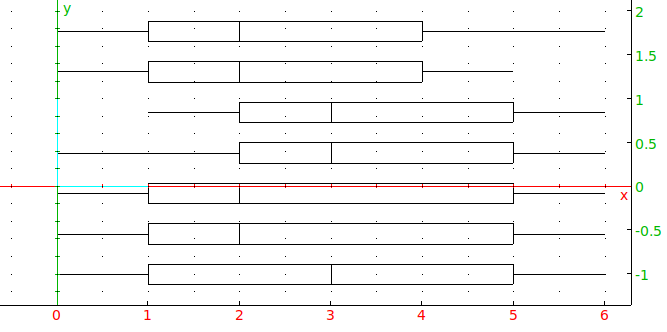
\includegraphics[width=0.75\textwidth]{xcas-boxwhiskermatrix.png}
\end{center}
\end{itemize}

\subsection{Dimension of a matrix: \texttt{dim}
\index{dim}}

The \texttt{dim} command finds the dimension of a matrix.
\begin{itemize}
  \item \texttt{dim} takes one argument:\\
  $A$, a matrix
  \item \texttt{dim($A$)} returns a list of the number of rows and columns of the matrix
  $A$.
\end{itemize}

\smallskip

\noindent
\textbf{Example.}\\
\textit{Input:}
\begin{center}
\texttt{dim([[1,2,3],[3,4,5]])}
\end{center}
\textit{Output:}
\[
\left[2,3\right]
\]
%begin{center}\texttt{[2,3]}\end{center}

\subsection{Number of rows: \texttt{rowdim} \texttt{rowDim} \texttt{nrows}
\index{rowdim}
\index{rowDim}
\index{nrows}}

The \texttt{rowdim} command finds the number of rows of a matrix.\\
\texttt{rowDim} and \texttt{nrows} are synonyms for \texttt{rowdim}.
\begin{itemize}
  \item \texttt{rowdim} takes one argument:\\
  $A$, a matrix.
  \item \texttt{rowdim($A$)} returns the number of rows of the matrix
  $A$.
\end{itemize}

\smallskip

\noindent
\textbf{Example.}\\
\textit{Input: }
\begin{center}
\texttt{rowdim([[1,2,3],[3,4,5]])}
\end{center}
% or:
% \begin{center}\texttt{nrows([[1,2,3],[3,4,5]])}\end{center}
\textit{Output:}
\[
2
\]
%\begin{center}\texttt{2}\end{center}

\subsection{Number of columns: \texttt{coldim} \texttt{colDim} \texttt{ncols}
\index{coldim}
\index{colDim}
\index{ncols}}


The \texttt{coldim} command finds the number of columns of a matrix.\\
\texttt{colDim} and \texttt{ncols} are synonyms for \texttt{coldim}.
\begin{itemize}
  \item \texttt{coldim} takes one argument:\\
  $A$, a matrix.
  \item \texttt{coldim($A$)} returns the number of columns of the matrix
  $A$.
\end{itemize}

\smallskip

\noindent
\textbf{Example.}\\
\textit{Input:}
\begin{center}
\texttt{coldim([[1,2,3],[3,4,5]])}
\end{center}
% or:
% \begin{center}\texttt{ncols([[1,2,3],[3,4,5]])}\end{center}
\textit{Output:}
\[
3
\]
%\begin{center}\texttt{3}\end{center}

\section{Sparse matrices}

\subsection{Defining sparse matrices
\label{ssec:spmatrices}}

A matrix is \emph{sparse} if most of its elements are 0.  To specify a
sparse matrix, it is easier to define the non-zero elements.
This can be done with a table (see \secref{sec:table}).
The \texttt{matrix} command (see \secref{ssec:matrixcommand}) or the
\texttt{convert} command (see \secref{ssec:convert}) can then
turn the table into a matrix.

\smallskip

\noindent
\textbf{Example.}\\
First, define the non-zero elements.\\
\textit{Input:}
\begin{center}
  \texttt{A:= table((0,0)=1, (1,1)=2, (2,2)=3, (3,3) = 4, (4,4) = 5)}
\end{center}
\textit{or:}
\begin{center}
\begin{tabular}{l}
  \texttt{purge(A)}\\
  \texttt{A[0..4,0..4]:=[1,2,3,4,5]}
\end{tabular}
\end{center}
\textit{Output:}
\[
\begin{array}{|c|c|}\hline\mathbf{Key}&\mathbf{Value}\\\hline \left(0,0\right)&1\\\hline \left(1,1\right)&2\\\hline \left(2,2\right)&3\\\hline \left(3,3\right)&4\\\hline \left(4,4\right)&5\\\hline \end{array}
\]
% \begin{center}
%   \tt
% table((0,0) = 1, (1,1) = 2, (2,2) = 3, (3,3) = 4, (4,4) = 5)
% \end{center}
This table can be converted to a matrix with either the
\texttt{convert} command or the \texttt{matrix} command.\\
\textit{Input:}
\begin{center}
  \texttt{a:= convert(A,array)}
\end{center}
\textit{or:}
\begin{center}
  \texttt{a:= matrix(A)}
\end{center}
\textit{Output:}
\[
\left[\begin{array}{ccccc}1&0&0&0&0\\0&2&0&0&0\\0&0&3&0&0\\0&0&0&4&0\\0&0&0&0&5\end{array}\right]
\]
% \begin{center}
%   \tt
%   [[1,0,0,0,0],[0,2,0,0,0],[0,0,3,0,0],[0,0,0,4,0],[0,0,0,0,5]]
% \end{center}

\subsection{Operations on sparse matrices}

All matrix operations can be done on tables that are used to define
sparse matrices.

\smallskip

\noindent
\textbf{Example.}\\
Create some sparse matrices.\\
\textit{Input:}
\begin{center}
\begin{tabular}{l}
  \texttt{purge(A):;}\\
  \texttt{A[0..2,0..2]:= [1,2,3]}
\end{tabular}
\end{center}
\textit{Output:}
\[
\begin{array}{|c|c|}\hline\mathbf{Key}&\mathbf{Value}\\\hline \left(0,0\right)&1\\\hline \left(1,1\right)&2\\\hline \left(2,2\right)&3\\\hline \end{array}
\]
% \begin{center}
%   \tt
% table((0,0) = 1, (1,1) = 2, (2,2) = 3)
% \end{center}
\textit{Input:}
\begin{center}
\begin{tabular}{l}
  \texttt{purge(B):;}\\
  \texttt{B[0..1,1..2]:= [1,2]:;}\\
  \texttt{B[0..2,0]:=5}
\end{tabular}
\end{center}
\textit{Output:}
\[
\begin{array}{|c|c|}\hline\mathbf{Key}&\mathbf{Value}\\\hline \left(0,0\right)&5\\\hline \left(0,1\right)&1\\\hline \left(1,0\right)&5\\\hline \left(1,2\right)&2\\\hline \left(2,0\right)&5\\\hline \end{array}
\]
% \begin{center}
%   \tt
% table((0,0) = 5, (0,1) = 1, (1,0) = 5, (1,2) = 2, (2,0) = 5)
% \end{center}
The usual operations will work on \texttt{A} and \texttt{B}.\\
\textit{Input:}
\begin{center}
  \texttt{A + B}
\end{center}
\textit{Output:}
\[
\begin{array}{|c|c|}\hline\mathbf{Key}&\mathbf{Value}\\\hline \left(0,0\right)&6\\\hline \left(0,1\right)&1\\\hline \left(1,0\right)&5\\\hline \left(1,1\right)&2\\\hline \left(1,2\right)&2\\\hline \left(2,0\right)&5\\\hline \left(2,2\right)&3\\\hline \end{array}
\]
% \begin{center}
%   \tt
%  table((0,0) = 6, (0,1) = 1, (1,0) = 5, (1,1) = 2, (1,2) = 2, (2,0) = 5, (2,2) = 3)
% \end{center}
\textit{Input:}
\begin{center}
  \texttt{A * B}
\end{center}
\textit{Output:}
\[
\begin{array}{|c|c|}\hline\mathbf{Key}&\mathbf{Value}\\\hline \left(0,0\right)&5\\\hline \left(0,1\right)&1\\\hline \left(1,0\right)&10\\\hline \left(1,2\right)&4\\\hline \left(2,0\right)&15\\\hline \end{array}
\]
% \begin{center}
%   \tt
%  table((0,0) = 5, (0,1) = 1, (1,0) = 10, (1,2) = 4, (2,0) = 15)
% \end{center}
\textit{Input:}
\begin{center}
  \texttt{2*A}
\end{center}
\textit{Output:}
\[
\begin{array}{|c|c|}\hline\mathbf{Key}&\mathbf{Value}\\\hline \left(0,0\right)&2\\\hline \left(1,1\right)&4\\\hline \left(2,2\right)&6\\\hline \end{array}
\]
% \begin{center}
%   \tt
%  table((0,0) = 2, (1,1) = 4, (2,2) = 6)
% \end{center}

\section{Linear algebra}

\subsection{Transpose of a matrix: \texttt{tran} \texttt{transpose}
\index{tran}
\index{transpose}
\label{ssec:transpose}}

The \texttt{tran} command finds the transpose of a matrix.\\
\texttt{transpose} is a synonym for \texttt{tran}.
\begin{itemize}
  \item \texttt{tran} takes one argument:\\
  $A$, a matrix.
  \item \texttt{tran($A$)} returns the transpose matrix of $A$.
\end{itemize}

\smallskip

\noindent
\textbf{Example.}\\
\textit{Input:}
\begin{center}
\texttt{tran([[1,2],[3,4]])}
\end{center}
\textit{Output:}
\[
\begin{pmatrix}1&3\\2&4\end{pmatrix}
\]
%\begin{center}\texttt{[[1,3],[2,4]]}\end{center}

\subsection{Inverse of a matrix: \texttt{inv} \texttt{/}
\index{inv|textbf}\index{/|textbf}\label{ssec:inv}}

The \texttt{inv} command finds the inverse of a matrix.
\begin{itemize}
  \item \texttt{inv} takes one argument:\\
  $A$, a matrix.
  \item \texttt{inv($A$)} returns the inverse matrix of $A$.
\end{itemize}
Note that \texttt{1/$A$} is another way to find the inverse of a matrix.

\smallskip

\noindent
\textbf{Example.}\\
\textit{Input:}
\begin{center}
\texttt{inv([[1,2],[3,4]])}
\end{center}
\textit{or:}
\begin{center}
\texttt{1/[[1,2],[3,4]]}
\end{center}
\textit{or:}
\begin{center}
\texttt{A:=[[1,2],[3,4]];1/A}
\end{center}
\textit{Output:}
\[
\left[\begin{array}{cc}-2&1\\\frac{3}{2}&-\frac{1}{2}\end{array}\right]
\]
%\begin{center}\texttt{[[-2,1],[3/2,1/-2]]}\end{center}

\subsection{Trace of a matrix: \texttt{trace}
\index{trace}}

The \emph{trace} of a square matrix is the sum of the diagonal
elements.  The \texttt{trace} command finds the trace of a matrix.
\begin{itemize}
  \item \texttt{trace} takes one argument:\\
  $A$, a matrix.
  \item \texttt{trace($A$)} returns the trace of the matrix $A$.
\end{itemize}

\smallskip

\noindent
\textbf{Example.}\\
\textit{Input:}
\begin{center}
\texttt{trace([[1,2],[3,4]])}
\end{center}
\textit{Output:}
\[
5
\]
%\begin{center}\texttt{5}\end{center}
%\end{itemize}

\subsection{Determinant of a matrix: \texttt{det}
\index{det|textbf}
\index{lagrange@\textit{lagrange}}
\index{rational\_det@\textit{rational\_det}}
\index{bareiss@\textit{bareiss}}
\index{linsolve@\textit{linsolve}}
\index{minor\_det@\textit{minor\_det}}
\label{ssec:det}}

The \texttt{det} command finds the determinant of a matrix.
\begin{itemize}
  \item \texttt{det} takes one mandatory argument and one optional
  argument:
  \begin{itemize}
    \item $A$, a matrix.
    \item Optionally, \textit{method}, which determines how the
    determinant will be computed and can be one of:
  \begin{itemize}
    \item \texttt{lagrange} When the matrix elements are polynomials or
    rational functions, this method computes the determinant by
    evaluating the elements and using Lagrange interpolation.
    \item \texttt{rational\_det}  This method uses Gaussian elimination
    without converting to to the internal format for fractions.
    \item \texttt{bareiss}  This uses the Gauss-Bareiss algorithm.
    \item \texttt{linsolve} This uses the $p$-adic algorithm for
    matrices with integer coefficients.
    \item \texttt{minor\_det} This uses expansion by minor determinants.
    This requires $2^n$ operations, but can stil be faster for average
    sized matrices (up to about $n=20$).
  \end{itemize}
  \end{itemize}
  \item \texttt{det($A\,\langle$}\textit{,method}$\rangle$\texttt{)}
  returns the determinant of the matrix $A$. 
\end{itemize}

\smallskip

\noindent
\textbf{Examples.}
\begin{itemize}
\item 
\textit{Input:}
\begin{center}
\texttt{det([[1,2],[3,4]])}
\end{center}
\textit{Output:}
\[
-2
\]
%\begin{center}\texttt{-2}\end{center}
\item
\textit{Input:}
\begin{center}
\texttt{det(idn(3))}
\end{center}
\textit{Output:}
\[
1
\]
%\begin{center}\texttt{1}\end{center}
\end{itemize}

\subsection{Determinant of a sparse matrix: \texttt{det\_minor}
\index{det\_minor}}

The \texttt{det\_minor} command finds the determinant of a matrix by
expanding the determinant using Laplace's algorithm.
\begin{itemize}
  \item \texttt{det\_minor} takes one argument:\\
  $A$, a matrix.
  \item \texttt{det\_minor($A$)} returns the determinant of the matrix
  $A$.
\end{itemize}

\smallskip

\noindent
\textbf{Examples.}
\begin{itemize}
\item 
\textit{Input:}
\begin{center}
\texttt{det\_minor([[1,2],[3,4]])}
\end{center}
\textit{Output:}
\[
-2
\]
%\begin{center}\texttt{-2}\end{center}
\item
\textit{Input:}
\begin{center}
\texttt{det\_minor(idn(3))}
\end{center}
\textit{Output:}
\[
1
\]
%\begin{center}\texttt{1}\end{center}
\end{itemize}

\subsection{Rank of a matrix: \texttt{rank}
\index{rank}}

The \texttt{rank} command finds the rank of a matrix.
\begin{itemize}
  \item \texttt{rank} takes one argument:\\
  $A$, a matrix.
  \item \texttt{rank($A$)} returns the rank of the matrix $A$.
\end{itemize}

\smallskip

\noindent
\textbf{Examples.}
\begin{itemize}
\item 
\textit{Input:}
\begin{center}
\texttt{rank([[1,2],[3,4]])}
\end{center}
\textit{Output:}
\[
2
\]
%\begin{center}\texttt{2}\end{center}
\item
\textit{Input:}
\begin{center}
\texttt{rank([[1,2],[2,4]])}
\end{center}
\textit{Output:}
\[
1
\]
%\begin{center}\texttt{1}\end{center}
\end{itemize}

\subsection{Transconjugate of a matrix: \texttt{trn}
\index{trn}}

The \emph{transconjugate} of a matrix is the conjugate of the
transpose of the matrix.  The \texttt{trn} command finds the
transconjugate of a matrix.
\begin{itemize}
  \item \texttt{trn} takes one argument:\\
  $A$, a matrix.
  \item \texttt{trn($A$)} returns the transconjugate of $A$.
\end{itemize}


\smallskip

\noindent
\textbf{Example.}\\
\textit{Input:}
\begin{center}
\texttt{trn([[i, 1+i],[1, 1-i]])}
\end{center}
\textit{Output:}
\[
\begin{pmatrix}-\mathrm{i}&1\\1-\mathrm{i}&1+\mathrm{i}\end{pmatrix}
\]
%\begin{center}\texttt{[[-i,1],[1-i,1+i]]}\end{center}

\subsection{Equivalent matrix: \texttt{changebase}
\index{changebase}}

The \texttt{changebase} command changes a matrix to represent the same
linear function in a different basis.
\begin{itemize}
  \item \texttt{changebase} takes two arguments:
  \begin{itemize}
    \item $A$, a matrix.
    \item $P$, a change-of-basis matrix.
  \end{itemize}
  \item \texttt{changebase($A,P$)} returns the matrix $P^{-1}AP$.
\end{itemize}

\smallskip

\noindent
\textbf{Examples.}
\begin{itemize}
\item 
\textit{Input:}
\begin{center}
\texttt{changebase([[1,2],[3,4]],[[1,0],[0,1]])}
\end{center}
\textit{Output:}
\[
\left[\begin{array}{cc}1&2\\3&4\end{array}\right]
\]
%\begin{center}\texttt{[[1,2],[3,4]]}\end{center}
\item
\textit{Input:}
\begin{center}
\texttt{changebase([[1,1],[0,1]],[[1,2],[3,4]])}
\end{center}
\textit{Output:}
\[
\left[\begin{array}{cc}-5&-8\\\frac{9}{2}&7\end{array}\right]
\]
%\begin{center}\texttt{[[-5,-8],[9/2,7]]}\end{center}
Indeed:
\[\left[\begin{array}{rr} 
    1 & 2\\
    3&4
  \end{array}\right]^{-1}\cdot
  \left[\begin{array}{rr}
  1 & 1\\
  0&1
  \end{array}\right]\cdot
  \left[\begin{array}{rr}1 & 2\\
  3&4\end{array}\right]=
  \left[\begin{array}{rr}
  -5 & -8\\
  \frac{9}{2}&7
  \end{array}\right]
\]
\end{itemize}

\subsection{Basis of a linear subspace : \texttt{basis}
\index{basis}}

The \texttt{basis} command finds a basis of a linear subspace of
$\mathbb{R}^{n}$ given a spanning set.
\begin{itemize}
  \item \texttt{basis} takes one argument:\\
  $L$, a list of vectors generating a linear subspace of $\mathbb R^n$.
  \item \texttt{basis($L$)} returns a list of vectors that is a basis
  of this linear subspace.
\end{itemize}

\smallskip

\noindent
\textbf{Example.}\\
\textit{Input: }
\begin{center}
\texttt{basis([[1,2,3],[1,1,1],[2,3,4]])}
\end{center}
\textit{Output:}
\[
\left\{\left[-1,0,1\right],\left[0,-1,-2\right]\right\}
\]
%\begin{center}\texttt{[[1,0,-1],\ [0,1,2]]}\end{center}

\subsection{Basis of the intersection of two subspaces: \texttt{ibasis}
\index{ibasis}}

The \texttt{ibasis} command finds a basis for the intersection of two
subspaces of $\mathbb{R}^{n}$.
\begin{itemize}
  \item \texttt{ibasis} takes two arguments:\\
  $L_{1}$ and $L_{2}$, two lists of vectors generating two subspaces
  of $\mathbb{R}^n$.
  \item \texttt{ibasis($L_{1},L_{2}$)} returns a
  list of vectors forming a basis for the intersection of these two
  subspaces.
\end{itemize}

\smallskip

\noindent
\textbf{Example.}\\
\textit{Input:}
\begin{center}
\texttt{ibasis([[1,2]],[[2,4]])}
\end{center}
\textit{Output:}
\[
\left\{\left[1,2\right]\right\}
\]
%\begin{center}\texttt{[[1,2]]}\end{center}

\subsection{Image of a linear function: \texttt{image}
\index{image}}

The \texttt{image} command finds a basis for the image of a linear
function.
\begin{itemize}
  \item \texttt{image} takes one argument:\\
  $A$, a matrix representing a linear function with respect to the
  standard basis.
  \item \texttt{image($A$)} returns a list of vectors that is a basis
  of the image of the linear function.
\end{itemize}

\smallskip

\noindent
\textbf{Example.}\\
\textit{Input:}
\begin{center}
\texttt{image([[1,1,2],[2,1,3],[3,1,4]])}
\end{center}
\textit{Output:}
\[
\left[\begin{array}{ccc}-1&0&1\\0&-1&-2\end{array}\right]
\]
%\begin{center}\texttt{[[-1,0,1],[0,-1,-2]]}\end{center}

\subsection{Kernel of a linear function: \texttt{kernel} \texttt{nullspace} \texttt{ker}
\index{ker}
\index{kernel}
\index{nullspace}}

The \texttt{ker} command finds a basis for the kernel of a linear
function.\\
\texttt{kernel} and \texttt{nullspace} are synonyms for \texttt{ker}.
\begin{itemize}
  \item \noindent\texttt{ker} takes one argument:\\
  $A$, a matrix representing a linear function with respect to the
  standard basis.
  \item \texttt{ker($A$)} returns a list of vectors that is a basis of
  the kernel of the linear function.
\end{itemize}

\smallskip

\noindent
\textbf{Example.}\\
\textit{Input:}
\begin{center}
\texttt{ker([[1,1,2],[2,1,3],[3,1,4]])}
\end{center}
\textit{Output:}
\[
\left[\begin{array}{ccc}1&1&-1\end{array}\right]
\]
% \begin{center}\texttt{[[1,1,-1]]}\end{center}
% The kernel is generated by the vector \texttt{[1,1,-1]}.

\subsection{Kernel of a linear function: \texttt{Nullspace}
\index{Nullspace}}

The \texttt{Nullspace} command is the inert form of \texttt{nullspace}.
\textbf{Warning:}\\
The \texttt{Nullspace} command is only useful in Maple mode.
(See \secref{ssec:lang}; you can get into \texttt{Maple} mode by 
hitting the state line red button then \texttt{Prog style}, then
choosing Maple and Apply).

\begin{itemize}
  \item \texttt{Nullspace} takes one argument:\\
  $A$, an integer matrix representing a linear function with respect
  to the standard basis.
  \item \texttt{Nullspace($A$) mod $p$} returns a list of
  vectors that is a basis for the kernel of the linear transformation 
  $\mathbb{Z}/p\mathbb{Z}[X]$.
\end{itemize}

\smallskip

\noindent
\textbf{Examples.}
\begin{itemize}
\item 
\textit{Input:}
\begin{center}
\texttt{Nullspace([[1,1,2],[2,1,3],[3,1,4]])}
\end{center}
\textit{Output:}
\[
\mathrm{nullspace}\left(\left[\begin{array}{ccc}1&1&2\\2&1&3\\3&1&4\end{array}\right]\right)
\]
%\begin{center}\texttt{nullspace([[1,1,2],[2,1,3],[3,1,4]])}\end{center}
\item
\textit{Input (in Maple mode):}
\begin{center}
\texttt{Nullspace([[1,2],[3,1]]) mod 5}
\end{center}
\textit{Output:}
\[
\left[2,-1\right]
\]
%\begin{center}\texttt{[2,-1]}\end{center}
In Xcas mode, the equivalent input is:\\
\textit{Input (in \texttt{Xcas} mode):}
\begin{center}
\texttt{nullspace([[1,2],[3,1]] \% 5)}
\end{center}
\textit{Output:}
\[
\left[\begin{array}{cc}2\mathbin{\%}5&-1\end{array}\right]
\]
%\begin{center}\texttt{[2\% 5,-1]}\end{center}
\end{itemize}

\subsection{Subspace generated by the columns of a matrix: \texttt{colspace}
\index{colspace}}

The \texttt{colspace} command finds a basis for the column space of a
matrix.
\begin{itemize}
  \item \texttt{colspace} takes one mandatory argument and one
  optional argument:
  \begin{itemize}
    \item $A$, a matrix.
    \item Optionally, \textit{var}, a variable name.
  \end{itemize}
  \item \texttt{colspace($A\,\langle$\textit{var}$\rangle$)} returns a
  matrix whose columns are a basis of the subspace generated by the
  columns of $A$.  With the optional argument \textit{var},
  \texttt{Xcas} will store the dimension of the subspace generated by 
  the columns of $A$.
\end{itemize}

\smallskip

\noindent
\textbf{Examples.}
\begin{itemize}
\item 
\textit{Input:}
\begin{center}
\texttt{colspace([[1,1,2],[2,1,3],[3,1,4]])}
\end{center}
\textit{Output:}
\[
\left[\begin{array}{cc}-1&0\\0&-1\\1&-2\end{array}\right]
\]
%\begin{center}\texttt{[[-1,0],[0,-1],[1,-2]]}\end{center}
\item
\textit{Input:}
\begin{center}
\texttt{colspace([[1,1,2],[2,1,3],[3,1,4]],dimension)}
\end{center}
\textit{Output:}
\[
\left[\begin{array}{cc}-1&0\\0&-1\\1&-2\end{array}\right]
\]
%\begin{center}\texttt{[[-1,0],[0,-1],[1,-2]]}\end{center}
\textit{then input:}
\begin{center}
\texttt{dimension}
\end{center}
\textit{Output:}
\[
2
\]
%\begin{center}\texttt{2}\end{center}
\end{itemize}

\subsection{Subspace generated by the rows of a matrix: \texttt{rowspace}
\index{rowspace}}

The \texttt{rowspace} command finds a basis for the row space of a
matrix.
\begin{itemize}
  \item \texttt{rowspace} takes one mandatory argument and one
  optional argument:
  \begin{itemize}
    \item $A$, a matrix.
    \item Optionally, \textit{var}, a variable name.
  \end{itemize}
  \item \texttt{rowspace($A\,\langle$\textit{var}$\rangle$)} returns a
  list of vectors which form a basis of the subspace generated by the
  rows of $A$.  With the optional argument \textit{var},
  \texttt{Xcas} will store the dimension of the subspace generated by 
  the rows of $A$.
\end{itemize}

\smallskip

\noindent
\textbf{Examples.}
\begin{itemize}
\item 
\textit{Input:}
\begin{center}
\texttt{rowspace([[1,1,2],[2,1,3],[3,1,4]])}
\end{center}
\textit{Output:}
\[
\left[\begin{array}{ccc}-1&0&-1\\0&-1&-1\end{array}\right]
\]
%\begin{center}\texttt{[[-1,0,-1],[0,-1,-1]]}\end{center}
\item
\textit{Input:}
\begin{center}
\texttt{rowspace([[1,1,2],[2,1,3],[3,1,4]],dimension)}
\end{center}
\textit{Output:}
\[
\left[\begin{array}{ccc}-1&0&-1\\0&-1&-1\end{array}\right]
\]
%\begin{center}\texttt{[[-1,0,-1],[0,-1,-1]]}\end{center}
\textit{then input:}
\begin{center}
\texttt{dimension}
\end{center}
\textit{Output:}
\[
2
\]
%\begin{center}\texttt{2}\end{center}
\end{itemize}

\section{Matrix reduction}

\subsection{Eigenvalues: \texttt{eigenvals}
\index{eigenvals}}

The \texttt{eigenvals} command finds eigenvalues of a matrix.
\begin{itemize}
  \item \texttt{eigenvals} takes one argument:\\
  $A$, a square matrix.
  \item \texttt{eigenvals($A$)} returns the sequence of the
  eigenvalues of $A$, including multiplicities.  (If $A$ is an
  $n\times n$ matrix, then the sequence will have $n$ values.)
\end{itemize}
\textbf{Remark:}
\texttt{Xcas} may not be able to find the exact roots of the
characteristic polynomial in some cases.  In that case,
\texttt{eigenvals($A$)} will return approximate eigenvalues of
$A$ if the coefficients are numeric or a subset of the eigenvalues if
the coefficients are symbolic.

\smallskip

\noindent
\textbf{Examples.}
\begin{itemize}
\item 
\textit{Input:}
\begin{center}
\texttt{eigenvals([[4,1,-2],[1,2,-1],[2,1,0]])}
\end{center}
\textit{Output:}
\[
2,2,2
\]
%\begin{center}\texttt{(2,2,2)}\end{center}
\item
\textit{Input:}
\begin{center}
\texttt{eigenvals([[4,1,0],[1,2,-1],[2,1,0]])}
\end{center}
\textit{Output:}
\[
\frac{\mathrm{rootof}\left(\left[\left[1,0,-20,0,100\right],\left[1,0,-24,0,144,0,-148\right]\right]\right)}{18},\frac{\mathrm{rootof}\left(\left[\left[-1,0,20,18,8\right],\left[1,0,-24,0,144,0,-148\right]\right]\right)}{36},\frac{\mathrm{rootof}\left(\left[\left[-1,0,20,-18,8\right],\left[1,0,-24,0,144,0,-148\right]\right]\right)}{36}
\]
%\texttt{eigenvals([[4,1,0],[1,2,-1],[2,1,0]])}
\textit{Input:}
\begin{center}
\texttt{evalf(eigenvals([[4,1,0],[1,2,-1],[2,1,0]]))}
\end{center}
\textit{Output:}
\[
1.46081112719,4.21431974338,0.324869129433
\]
%\begin{center}\texttt{(0.324869129433,4.21431974338,1.46081112719)}\end{center}
\end{itemize}

\subsection{Eigenvalues: \texttt{egvl} \texttt{eigenvalues} \texttt{eigVl}
\index{egvl}
\index{eigVl}
\index{eigenvalues}}

The \texttt{egvl} command finds the Jordan form of a matrix.\\
\texttt{eigenvalues} and \texttt{eigVl} are synonyms for \texttt{egvl}.
\begin{itemize}
  \item \texttt{egvl} takes one argument:\\
  $A$, a square matrix.
  \item \texttt{egvl($A$)} returns the Jordan normal form of $A$.
\end{itemize}
% \textbf{Remark}: If $A$ is exact, \texttt{Xcas} may not be able to
% find the exact roots of the characteristic polynomial,
% \texttt{eigenvalues} will return an approximate diagonalization of $A$
% if the coefficients are numeric.\\ 

\smallskip

\noindent
\textbf{Examples.}
\begin{itemize}
\item
\textit{Input:}
\begin{center}
\texttt{egvl([[4,1,-2],[1,2,-1],[2,1,0]])}
\end{center}
\textit{Output:}
\[
\left[\begin{array}{ccc}2&1&0\\0&2&1\\0&0&2\end{array}\right]
\]
%\begin{center}\texttt{[[2,1,0],[0,2,1],[0,0,2]]}\end{center}
\item
\textit{Input:}
\begin{center}
\texttt{egvl([[4,1,0],[1,2,-1],[2,1,0]])}
\end{center}
\textit{Output:}\\
See \secref{ssec:rootof} for a discussion of \texttt{rootof}.
\[
\left[\begin{array}{ccc}\frac{\mathrm{rootof}\left(\left[\left[1,0,-20,0,100\right],\left[1,0,-24,0,144,0,-148\right]\right]\right)}{18}&0&0\\0&\frac{\mathrm{rootof}\left(\left[\left[-1,0,20,18,8\right],\left[1,0,-24,0,144,0,-148\right]\right]\right)}{36}&0\\0&0&\frac{\mathrm{rootof}\left(\left[\left[-1,0,20,-18,8\right],\left[1,0,-24,0,144,0,-148\right]\right]\right)}{36}\end{array}\right]
\]
\textit{Input:}
\begin{center}
\texttt{evalf(egvl([[4,1,0],[1,2,-1],[2,1,0]]))}
\end{center}
\textit{Output:}
\[
\left[\begin{array}{ccc}1.46081112719&0.0&0.0\\0.0&4.21431974338&0.0\\0.0&0.0&0.324869129433\end{array}\right]
\]
\end{itemize}

\subsection{Eigenvectors: \texttt{egv} \texttt{eigenvectors} \texttt{eigenvects} \texttt{eigVc}
\index{egv}
\index{eigenvectors}
\index{eigenvects}
\index{eigVc}}

The \texttt{egv} command finds the eigenvectors of a diagonalizable
matrix.\\
\texttt{eigenvectors}, \texttt{eigenvects} and \texttt{eigVc} are
synonyms for \texttt{egv}.
\begin{itemize}
  \item \texttt{egv} takes one argument:\\
  $A$, a square matrix.
  \item \texttt{egv($A$)} returns a matrix whose columns are the
  eigenvectors of the matrix $A$ if $A$ is diagonalizable, otherwise
  it will fail.
\end{itemize}
See also \secref{ssec:jordan} for characteristic vectors.

\smallskip

\noindent
\textbf{Examples.}
\begin{itemize}
\item 
\textit{Input:}
\begin{center}
\texttt{egv([[1,1,3],[1,3,1],[3,1,1]])}
\end{center}
\textit{Output:}
\[
\left[\begin{array}{ccc}1&-1&1\\1&2&0\\1&-1&-1\end{array}\right]
\]
%\begin{center}\texttt{[[-1,1,1],[2,1,0],[-1,1,-1]]}\end{center}
\item
\textit{Input:}
\begin{center}
\texttt{egv([[4,1,-2],[1,2,-1],[2,1,0]])}
\end{center}
\textit{Output:}
\begin{center}
\texttt{"Not diagonalizable at eigenvalue 2"}
\end{center}
\item 
\textit{Input (in complex mode):}
\begin{center}
\texttt{egv([[2,0,0],[0,2,-1],[2,1,2]])}
\end{center}
\textit{Output:}
\[
\left[\begin{array}{ccc}1&0&0\\-2&-1&-1\\0&-\mathrm{i}&\mathrm{i}\end{array}\right]
\]
%\begin{center}\texttt{[0,1,0],[-1,-2,-1],[i,0,-i]]}\end{center}
\end{itemize}

\subsection{Rational Jordan matrix: \texttt{rat\_jordan}
\index{rat\_jordan}}

The \texttt{rat\_jordan} command finds the rational Jordan form of a
matrix.
\begin{itemize}
  \item \texttt{rat\_jordan} takes one mandatory and one optional
  argument:
  \begin{itemize}
    \item $A$, a square matrix (preferably with exact coefficients).
    \item Optionally, \textit{var}, a variable name.
  \end{itemize}
  \item
  \texttt{rat\_jordan($A$)} (in all modes but \texttt{Maple}) returns
  a sequence $[P,J]$ of two matrices, where $J$ is the rational Jordan
  matrix of $A$ (the most reduced matrix in the field of the
  coefficients of $A$ or the complexified field in complex mode) and
  \[ 
  J=P^{-1}AP 
  \]
  The coefficients of $P$ and $J$ belongs to the same field as the
  coefficients of $A$.
  If A is diagonalizable in the field of its coefficients, then the
  columns of $P$ are the eigenvectors of $A$.
  
  \smallskip
  
  \texttt{rat\_jordan($A$)} (in \texttt{Maple} mode) only returns the
  matrix $J$.
  \item
  \texttt{rat\_jordan($A\,\langle$}\textit{var}$\rangle$\texttt{)}
  returns the matrix $J$, as above, and assigns the matrix $P$ to the
  variable \textit{var}.
\end{itemize}

\smallskip

\noindent
\textbf{Examples.}
\begin{itemize}
\item 
\textit{Input (not in \texttt{Maple} mode):}
\begin{center} 
\texttt{rat\_jordan([[1,0,0],[1,2,-1],[0,0,1]])}
\end{center}
\[
\left[\begin{array}{ccc}0&1&0\\1&0&1\\0&1&1\end{array}\right],\left[\begin{array}{ccc}2&0&0\\0&1&0\\0&0&1\end{array}\right]
\]
\item 
\textit{Input:}
\begin{center} 
\texttt{rat\_jordan([[1,0,0],[1,2,-1],[0,0,1]],P)}
\end{center}
\[
\left[\begin{array}{ccc}2&0&0\\0&1&0\\0&0&1\end{array}\right]
\]
\textit{then input:}
\begin{center}
  \texttt{P}
\end{center}
\textit{Output:}
\[
\left[\begin{array}{ccc}0&1&0\\1&0&1\\0&1&1\end{array}\right]
\]
%\end{itemize}
%\item the coefficients of $P$ and $J$ belongs to the same field as the
%coefficients of $A$.\\
%For example, in \texttt{Xcas} mode, input:
\item
\textit{Input:}
\begin{center} 
\texttt{rat\_jordan([[1,0,1],[0,2,-1],[1,-1,1]])}
\end{center}
\textit{Output:}
\[
\left[\begin{array}{ccc}1&1&2\\0&0&-1\\0&1&2\end{array}\right],\left[\begin{array}{ccc}0&0&-1\\1&0&-3\\0&1&4\end{array}\right]
\]
%\begin{center} \texttt{[[1,1,2],[0,0,-1],[0,1,2]],[[0,0,-1],[1,0,-3],[0,1,4]]}\end{center}
%\item
% \textit{Input:}\\
% (See \secref{ssec:compagne} for a discussion of \texttt{companion}.)
% \begin{center} 
% \texttt{companion(pcar([[1,0,1],[0,2,-1],[1,-1,1]],x),x)}
% \end{center}
% \textit{Output:}
% \[
% \left[\begin{array}{ccc}0&0&-1\\1&0&-3\\0&1&4\end{array}\right]
%\]
%\begin{center} \texttt{[[0,0,-1],[1,0,-3],[0,1,4]]}\end{center}
\item
\textit{Input:}
\begin{center} 
\texttt{rat\_jordan([[1,0,0],[0,1,1],[1,1,-1]])}
\end{center}
\textit{Output:}
\[
\left[\begin{array}{ccc}-1&0&0\\1&1&1\\0&0&1\end{array}\right],\left[\begin{array}{ccc}1&0&0\\0&0&2\\0&1&0\end{array}\right]
\]
%\begin{center} \texttt{[[-1,0,0],[1,1,1],[0,0,1]],[[1,0,0],[0,0,2],[0,1,0]]}\end{center}
% \item
% Input:
% \begin{center} \texttt{factor(pcar([[1,0,0],[0,1,1],[1,1,-1]],x))}\end{center}
% Output:
% \begin{center} \texttt{-(x-1)*(x\^{}2-2)}\end{center}
% Input:
% \begin{center} \texttt{companion((x\^{}2-2),x)}\end{center}
% Output:
% \begin{center} \texttt{[[0,2],[1,0]]}\end{center}
\end{itemize}

\smallskip

If $A$ is symmetric and has eigenvalues with multiple orders,
the matrix $P$ returned by \texttt{rat\_jordan($A$)} will contain
orthogonal eigenvectors (not always of norm equal to 1); i.e.,
\texttt{tran($P$)*$P$} will be a diagonal matrix where the diagonal is the
square norm of the eigenvectors. 

\smallskip

\noindent
\textbf{Example.}\\
\textit{Input:}
\begin{center} 
\texttt{rat\_jordan([[4,1,1],[1,4,1],[1,1,4]])}
\end{center}
\textit{Output:}
\[
\left[\begin{array}{ccc}1&2&-1\\1&0&2\\1&-2&-1\end{array}\right],\left[\begin{array}{ccc}6&0&0\\0&3&0\\0&0&3\end{array}\right]
\]
%\begin{center} \texttt{[[1,-1,1/2],[1,0,-1],[1,1,1/2]],[[6,0,0],[0,3,0],[0,0,3]]}
%\end{center}
% \end{itemize}
% Input in \texttt{Xcas}, \texttt{Mupad} or \texttt{TI} mode:
% \begin{center}\texttt{rat\_jordan([[1,0,0],[1,2,-1],[0,0,1]])}\end{center}
% Output:
% \begin{center}\texttt{[[0,1,0],[1,0,1],[0,1,1]],[[2,0,0],[0,1,0],[0,0,1]]}\end{center}
% Input in \texttt{Xcas}, \texttt{Mupad} or \texttt{TI} mode:
% \begin{center}\texttt{rat\_jordan([[4,1,-2],[1,2,-1],[2,1,0]])}\end{center}
% Output:
% \begin{center}\texttt{[[[1,2,1],[0,1,0],[1,2,0]],[[2,1,0],[0,2,1],[0,0,2]]]}\end{center}
% In complex mode and in \texttt{Xcas}, \texttt{Mupad} or \texttt{TI} mode , input:
% \begin{center}\texttt{rat\_jordan([[2,0,0],[0,2,-1],[2,1,2]])}\end{center}
% Output:
% \begin{center}\texttt{[[1,0,0],[-2,-1,-1],[0,-i,i]],[[2,0,0],[0,2-i,0],[0,0,2+i]]}\end{center}
% Input  in \texttt{Maple} mode:
% \begin{center}\texttt{rat\_jordan([[1,0,0],[1,2,-1],[0,0,1]],'P')}\end{center}
% Output:
% \begin{center}\texttt{[[2,0,0],[0,1,0],[0,0,1]]}\end{center}
% then input:
% \begin{center}\texttt{P}\end{center}
% Output:
% \begin{center}\texttt{[[0,1,0],[1,0,1],[0,1,1]]]}\end{center}

\subsection{Jordan normal form: \texttt{jordan}
\index{jordan}
\label{ssec:jordan}}

The \texttt{jordan} command finds the Jordan form of a
matrix.
\begin{itemize}
  \item \texttt{jordan} takes one mandatory and one optional
  argument:
  \begin{itemize}
    \item $A$, a square matrix.
    \item Optionally, \textit{var}, a variable name.
  \end{itemize}
  \item
  \texttt{jordan($A$)} (in all modes but \texttt{Maple}) returns
  a sequence $[P,J]$ of two matrices, where the columns of $P$ are the
  eigenvectors of $A$, $J$ is the Jordan form of $A$, and
  \[ 
  J=P^{-1}AP 
  \]
  
  \smallskip
  
  \texttt{jordan($A$)}, in \texttt{Maple} mode, only returns the
  matrix $J$.
  \item
  \texttt{jordan($A\,\langle$}\textit{var}$\rangle$\texttt{)}
  returns the matrix $J$, as above, and assigns the matrix $P$ to the
  variable \textit{var}.
\end{itemize}

\smallskip

\noindent
\textbf{Examples.}
\begin{itemize}
\item 
\textit{Input (not in \texttt{Maple} mode):}
\begin{center} 
\texttt{jordan([[4,1,1],[1,4,1],[1,1,4]])}
\end{center}
\textit{Output:}
\[
\left[\begin{array}{ccc}1&2&-1\\1&0&2\\1&-2&-1\end{array}\right],\left[\begin{array}{ccc}6&0&0\\0&3&0\\0&0&3\end{array}\right]
\]
\item 
\textit{Input:}
\begin{center} 
\texttt{jordan([[4,1,1],[1,4,1],[1,1,4]],P)}
\end{center}
\textit{Output:}
\[
\left[\begin{array}{ccc}6&0&0\\0&3&0\\0&0&3\end{array}\right]
\]
%\begin{center} \texttt{[[1,-1,1/2],[1,0,-1],[1,1,1/2]]}
%\end{center}
\textit{then input:}
\begin{center}
\texttt{P}  
\end{center}
\textit{Output:}
\[
\left[\begin{array}{ccc}1&2&-1\\1&0&2\\1&-2&-1\end{array}\right]
\]
\end{itemize}


\smallskip

If $A$ is symmetric and has eigenvalues with multiple orders,
the matrix $P$ returned by \texttt{jordan($A$)} will contain
orthogonal eigenvectors (not always of norm equal to 1); i.e.,
\texttt{tran($P$)*$P$} will be a diagonal matrix where the diagonal is
the square norm of the eigenvectors. 

\smallskip

\noindent
\textbf{Example:}\\
\textit{Input:}
\begin{center} 
\texttt{jordan([[4,1,1],[1,4,1],[1,1,4]])}
\end{center}
\textit{Output:}
\[
\left[\begin{array}{ccc}1&2&-1\\1&0&2\\1&-2&-1\end{array}\right],\left[\begin{array}{ccc}6&0&0\\0&3&0\\0&0&3\end{array}\right]
\]

 % Input in \texttt{Xcas}, \texttt{Mupad} or \texttt{TI} mode:
% \begin{center}\texttt{jordan([[1,0,0],[0,1,1],[1,1,-1]])}\end{center}
% Output:
% \begin{center}\texttt{[[1,0,0],[0,1,1],[1,1,-1]],[[-1,0,0],[1,1,1],[0,-sqrt(2)-1,sqrt(2)-1]],[[1,0,0],[0,-(sqrt(2)),0],[0,0,sqrt(2)]]}\end{center}
% Input  in \texttt{Maple} mode:
% \begin{center}\texttt{jordan([[1,0,0],[0,1,1],[1,1,-1]])}\end{center}
% Output:
% \begin{center}\texttt{[[1,0,0],[0,-(sqrt(2)),0],[0,0,sqrt(2)]]}\end{center}
% then input:
% \begin{center}\texttt{P}\end{center}
% Output:
% \begin{center}\texttt{[[-1,0,0],[1,1,1],[0,-sqrt(2)-1,sqrt(2)-1]]}\end{center}
% Input  in \texttt{Xcas}, \texttt{Mupad} or \texttt{TI} mode:
% \begin{center}\texttt{jordan([[4,1,-2],[1,2,-1],[2,1,0]])}\end{center}
% Output:
% \begin{center}\texttt{[[[1,2,1],[0,1,0],[1,2,0]],[[2,1,0],[0,2,1],[0,0,2]]]}\end{center}
% In complex mode and in \texttt{Xcas}, \texttt{Mupad} or \texttt{TI} mode , input:
% \begin{center}\texttt{jordan([[2,0,0],[0,2,-1],[2,1,2]])}\end{center}
% Output:
% \begin{center}\texttt{[[1,0,0],[-2,-1,-1],[0,-i,i]],[[2,0,0],[0,2-i,0],[0,0,2+i]]}\end{center}

\subsection{Powers of a square matrix: \texttt{matpow}
\index{matpow}}

The \texttt{matpow} command finds the power of a square matrix,
computed using the Jordan form.
\begin{itemize}
  \item \texttt{matpow} command takes two arguments:
  \begin{itemize}
    \item $A$, a square matrix.
    \item $n$, an integer.
  \end{itemize}
  \item \texttt{matpow($A,n$)} returns $A^{n}$.
\end{itemize}

\smallskip

\noindent
\textbf{Example.}\\
\textit{Input:}
\begin{center}
  \texttt{matpow([[1,2],[2,1]],n)}
\end{center}
\textit{Output:}
\[
\left[\begin{array}{cc}\frac{3^{n}+\left(-1\right)^{n}}{2}&\frac{3^{n}-\left(-1\right)^{n}}{2}\\\frac{3^{n}-\left(-1\right)^{n}}{2}&\frac{3^{n}+\left(-1\right)^{n}}{2}\end{array}\right]
\]
% \begin{center}
%   \tt
%   [[(3\^{}n+(-1)\^{}n)/2,(3\^{}n-(-1)\^{}n)/2],[(3\^{}n-(-1)\^{}n)/2,(3\^{}n+(-1)\^{}n)/2]]

% \end{center}

\smallskip

Notice that \texttt{jordan([[1,2],[2,1]])} returns
\[
\left[\begin{array}{cc}1&-1\\1&1\end{array}\right],\left[\begin{array}{cc}3&0\\0&-1\end{array}\right]
\]

\subsection{Characteristic polynomial: \texttt{charpoly}
\index{pcar}\index{charpoly}}

The \emph{characteristic polynomial} of a square matrix $A$ is the
polynomial 
\[ 
P(x)=\det(x I-A) 
\]
The \texttt{charpoly} command finds the characteristic polynomial of a
matrix.\\
\texttt{pcar} is a synonym for \texttt{charpoly}.
\begin{itemize}
  \item \texttt{charpoly} takes one mandatory argument and one
  optional argument:
  \begin{itemize}
    \item $A$, a square matrix.
    \item Optionally, $x$, a variable name.
  \end{itemize}
  \item \texttt{charpoly($A\,\langle x\rangle$)} returns the characteristic
  polynomial of $A$.  It is written as the list of its coefficients if no
  variable name was provided or written as an expression with respect to
  $x$ if there is a second argument.
\end{itemize}

\smallskip

\noindent
\textbf{Examples.}
\begin{itemize}
\item 
\textit{Input:}
\begin{center}
\texttt{charpoly([[4,1,-2],[1,2,-1],[2,1,0]])}
\end{center}
\textit{Output:}
\[
\left[1,-6,12,-8\right]
\]
%\begin{center}{\tt[1,-6,12,-8]}\end{center}
Hence, the characteristic polynomial of this matrix is
$x^3-6x^2+12x-8$.
\item
\textit{Input:}
\begin{center}
\texttt{charpoly([[4,1,-2],[1,2,-1],[2,1,0]],X)}
\end{center}
\textit{Output:}
\[
X^{3}-6 X^{2}+12 X-8
\]
%\begin{center}\texttt{X\^{}3-6*X\^{}2+12*X-8}\end{center}
\end{itemize}

\subsection{Characteristic polynomial using Hessenberg algorithm: \texttt{pcar\_hessenberg}
 \index{pcar\_hessenberg}}

The \texttt{pcar\_hessenberg} command finds the characteristic polynomial of a
matrix.  It computes the polynomial using the Hessenberg algorithm
(see e.g. Henri Cohen, \textsl{A Course in Computational Algebraic
Number Theory}) which is more efficient ($O(n^3)$ deterministic) if
the coefficients of the matrix are in a finite field or use a finite
representation like approximate numeric coefficients. Note however that
this algorithm behaves badly if the coefficients are, for example, in
$\mathbb{Q}$.
\begin{itemize}
  \item \texttt{pcar\_hessenberg} takes one mandatory argument and one
  optional argument:
  \begin{itemize}
    \item $A$, a square matrix.
    \item Optionally, $x$, a variable name.
  \end{itemize}
  \item \texttt{pcar\_hessenberg($A\,\langle x\rangle$)} returns the characteristic
  polynomial of $A$.  It is written as the list of its coefficients if no
  variable name was provided or written as an expression with respect to
  $x$ if there is a second argument.
\end{itemize}

\smallskip

\noindent
\textbf{Examples.}
\begin{itemize}
\item 
\textit{Input:}
\begin{center}
\texttt{pcar\_hessenberg([[4,1,-2],[1,2,-1],[2,1,0]] \% 37)}
\end{center}
\textit{Output:}
\[
\left[1\mathbin{\%}37,\left(-6\right)\mathbin{\%}37,12\mathbin{\%}37,\left(-8\right)\mathbin{\%}37\right]
\]
%\begin{center}\texttt{[1 \% 37 ,-6\% 37,12 \% 37,-8 \% 37]}\end{center}
\item
\textit{Input:}
\begin{center}
\texttt{pcar\_hessenberg([[4,1,-2],[1,2,-1],[2,1,0]] \% 37,x)}
\end{center}
\textit{Output:}
\[
\left(1\mathbin{\%}37\right) x^{3}+\left(\left(-6\right)\mathbin{\%}37\right) x^{2}+\left(12\mathbin{\%}37\right) x+\left(-8\right)\mathbin{\%}37
\]
%\begin{center}\texttt{x\^{}3-6 \%37 *x\^{}2+12 \% 37 *x-8 \% 37}\end{center}
Hence, the characteristic polynomial of [[4,1,-2],[1,2,-1],[2,1,0]] in
$\mathbb Z/37 \mathbb Z$ is $x^3-6x^2+12x-8$.
\end{itemize}

\subsection{Minimal polynomial: \texttt{pmin}
\index{pmin}}

The minimal polynomial of a square matrix $A$ is the polynomial $P$
having minimal degree such that $P(A)=0$.
The \texttt{pmin} command finds the minimal polynomial of a
matrix.
\begin{itemize}
  \item \texttt{pmin} takes one mandatory argument and one
  optional argument:
  \begin{itemize}
    \item $A$, a square matrix.
    \item Optionally, $x$, a variable name.
  \end{itemize}
  \item \texttt{pmin($A\,\langle x\rangle$)} returns the minimal
  polynomial $A$.  It is written as the list of its coefficients if no
  variable name was provided or written as an expression with respect to
  $x$ if there is a second argument.
\end{itemize}

\smallskip

\noindent
\textbf{Examples.}
\begin{itemize}
\item 
\textit{Input:}
\begin{center}
\texttt{pmin([[1,0],[0,1]])}
\end{center}
\textit{Output:}
\[
\left[1,-1\right]
\]
%\begin{center}\texttt{[1,-1]}\end{center}
\item
\textit{Input:}
\begin{center}
\texttt{pmin([[1,0],[0,1]],x)}
\end{center}
\textit{Output:}
\[
x-1
\]
%\begin{center}\texttt{x-1}\end{center}
Hence the minimal polynomial of [[1,0],[0,1]] is $x-1$.
\item
\textit{Input:}
\begin{center}
\texttt{pmin([[2,1,0],[0,2,0],[0,0,2]])}
\end{center}
\textit{Output:}
\[
\left[1,-4,4\right]
\]
%\begin{center}\texttt{[1,-4,4]}\end{center}
\item
\textit{Input:}
\begin{center}
\texttt{pmin([[2,1,0],[0,2,0],[0,0,2]],x)}
\end{center}
\textit{Output:}
\[
x^{2}-4 x+4
\]
%\begin{center}\texttt{x\^{}2-4*x+4}\end{center}
Hence, the minimal polynomial of [[2,1,0],[0,2,0],[0,0,2]] is $x^2-4x+4$.
\end{itemize}

\subsection{Adjoint matrix: \texttt{adjoint\_matrix}
\index{adjoint\_matrix}}

The \textit{comatrix} of a square matrix $A$ of size $n$ is the matrix
$B$ defined by $A\times B=\det(A)\times I$. The \textit{adjoint}
matrix $Q(x)$ of $A$ is the comatrix of $xI-A$. It is a polynomial of degree
$n-1$ in $x$ having matrix coefficients and satisfies:
\[
(xI-A)Q(x) = \det(xI-A)I= P(x)\times I
\] 
where $P(x)$ is the characteristic polynomial of $A$.
Since the polynomial $P(x)\times I-P(A)$ (with matrix coefficients) is
also divisible by $x\times I-A$ (by algebraic identities), this means
that $P(A)=0$. We also have $Q(x)\ =\ I\times x^{n-1}+\ldots+B_0$
where $B_0=$ is the comatrix of $A$ (times -1 if $n$ is odd).

The \texttt{adjoint\_matrix} command finds the characteristic
polynomial and adjoint of a given matrix.
\begin{itemize}
  \item \texttt{adjoint\_matrix} takes one argument:\\
  $A$, a square matrix.
  \item \texttt{adjoint\_matrix($A$)} returns the list of the
  coefficients of $P(x)$ (the characteristic polynomial of $A$), and the
  list of the matrix coefficients of $Q(x)$ (the adjoint matrix of $A$).
\end{itemize}

\smallskip

\noindent
\textbf{Examples.}
\begin{itemize}
\item 
\textit{Input:}
\begin{center}
\texttt{adjoint\_matrix([[4,1,-2],[1,2,-1],[2,1,0]])}
\end{center}
\textit{Output:}
\[
\left[\left[1,-6,12,-8\right],\left[\left[\begin{array}{ccc}1&0&0\\0&1&0\\0&0&1\end{array}\right],\left[\begin{array}{ccc}-2&1&-2\\1&-4&-1\\2&1&-6\end{array}\right],\left[\begin{array}{ccc}1&-2&3\\-2&4&2\\-3&-2&7\end{array}\right]\right]\right]
\]
% \begin{center}
% \texttt{[
%   \textbf{[}1,-6,12,-8\textbf{]},\\
% \textbf{[} [[1,0,0],[0,1,0],[0,0,1]],
%   [[-2,1,-2], [1,-4,-1],[2,1,-6]],
%   [[1,-2,3],[-2,4,2],[-3,-2,7]] \textbf{]}
% ]}\end{center}
Hence the characteristic polynomial is:
\[ 
P(x)=x^3-6*x^2+12*x-8 
\]
The determinant of $A$ is equal to $-P(0)=8$.
The comatrix of $A$ is equal to:
\[ 
B=Q(0)=
\left[\begin{array}{ccc} 
1 & -2 & 3\\ -2& 4 & 2\\ -3 & -2 & 7
\end{array}\right] 
\]
Hence the inverse of $A$ is equal to:
\[ 
\frac{1}{8}
\left[\begin{array}{ccc} 
1 & -2 & 3\\ -2& 4 & 2\\ -3 & -2 & 7
\end{array}\right] 
\]
%1/8*[[1,-2,3],[-2,4,2],[-3,-2,7]] \]
The adjoint matrix of $A$ is:
\[ 
\left[\begin{array}{ccc}x^{2}-2 x+1&x-2&-2 x+3\\x-2&x^{2}-4 x+4&-x+2\\2 x-3&x-2&x^{2}-6 x+7\end{array}\right]
%[[x^2-2x+1,x-2,-2x+3],[x-2,x^2-4x+4,-x+2],[2x-3,x-2,x^2-6x+7]] 
\]
\item
\textit{Input:}
\begin{center}
\texttt{adjoint\_matrix([[4,1],[1,2]])}
\end{center}
\textit{Output:}
\[
\left[\left[1,-6,7\right],\left[\left[\begin{array}{cc}1&0\\0&1\end{array}\right],\left[\begin{array}{cc}-2&1\\1&-4\end{array}\right]\right]\right]
\]
%\begin{center}{\tt[[1,-6,7],[[[1,0],[0,1]],[[-2,1],[1,-4]]]]}\end{center}
Hence the characteristic polynomial $P$ is:
\[ 
P(x)=x^2-6*x+7 
\]
The determinant of $A$ is equal to $+P(0)=7$.
The comatrix of $A$ is equal to
\[ 
Q(0)= -\left[\begin{array}{cc} -2& 1\\ 1& -4\end{array}\right]
\]
Hence the inverse of $A$ is equal to:
\[ 
-\frac{1}{7}\left[\begin{array}{cc} -2& 1\\ 1& -4\end{array}\right]
\]
%\[ -1/7*[[-2,1],[1,-4]] \]
The adjoint matrix of $A$ is:
%\[ -[[x-2,1],[1,x-4]] \]
\[
- \left[\begin{array}{cc}x-2&1\\1&x-4\end{array}\right]
\]
\end{itemize}

\subsection{Companion matrix of a polynomial: \texttt{companion}\label{ssec:compagne}
\index{companion|textbf}}

The \texttt{companion} command finds a matrix given its characteristic
polynomial; specifically, if the polynomial is
$P(x)=x^n+a_{n-1}x^{n-1}+\ldots+a_{-1}x+a_0$, this matrix is equal to 
the identity matrix of size $n-1$ bordered with $[0,0..,0,-a_0]$ as first
row, and with $[-a_0,-a_1,\ldots,-a_{n-1}]$ as last column.
\begin{itemize}
  \item \texttt{companion} takes two arguments:
  \begin{itemize}
    \item $P$, a unitary polynomial.
    \item $x$, the name of its variable.
  \end{itemize}
  \item \texttt{companion($P,x$)} returns the matrix whose characteristic polynomial is $P$.
\end{itemize}

\smallskip

\noindent
\textbf{Examples.}
\begin{itemize}
\item 
\textit{Input:}
\begin{center}
\texttt{companion(x\^{}2+5x-7,x)}
\end{center}
\textit{Output:}
\[
\left[\begin{array}{cc}0&7\\1&-5\end{array}\right]
\]
%\begin{center}\texttt{[[0,7],[1,-5]]}\end{center}
\item
\textit{Input:}
\begin{center}
\texttt{companion(x\^{}4+3x\^{}3+2x\^{}2+4x-1,x)}
\end{center}
\textit{Output:}
\[
\left[\begin{array}{cccc}0&0&0&1\\1&0&0&-4\\0&1&0&-2\\0&0&1&-3\end{array}\right]
\]
%\begin{center}\texttt{[[0,0,0,1],[1,0,0,-4],[0,1,0,-2],[0,0,1,-3]]}\end{center}
\end{itemize}

\subsection{Hessenberg matrix reduction: \texttt{hessenberg} \texttt{SCHUR}
\index{hessenberg}
\index{SCHUR}}

A \emph{Hessenberg} matrix is a square matrix where the coefficients
below the sub-principal diagonal are all 0s.  The \texttt{hessenberg}
command finds a Hessenberg matrix equivalent to a given square matrix.
\begin{itemize}
  \item \texttt{hessenberg} takes one mandatory argument and one
  optional argument:
  \begin{itemize}
    \item $A$, a matrix.
    \item $n$, an integer, either $0$, $-1$, $-2$ or a prime number
    greater than $1$ (by default $n=0$).
  \end{itemize}
  \item \texttt{hessenberg($A\,\langle n \rangle$)} returns a list
  $[P,B]$ with $B=P^{-1}AP$ and: 
  \begin{itemize}
    \item if $n=0$, $B$ is a Hessenberg matrix.
    \item if $n=-1$, the calculations are approximate and $B$ is upper
    triangular.
    \item if $n=-2$, the calculations are approximate, $P$ is
    orthogonal and $B$ has zero sub-subdiagonal elements.    
  \end{itemize}
\end{itemize}
\texttt{SCHUR($A$)} is equivalent to \texttt{hessenberg($A$,-1)},
which is compatible with HP calculators. 

\smallskip

\noindent
\textbf{Examples.}
\begin{itemize}
\item 
\textit{Input:}
\begin{center}
\begin{tabular}{l}
\texttt{A:=[[3,2,2,2,2],[2,1,2,-1,-1],[2,2,1,-1,1],[2,-1,-1,3,1],[2,-1,1,1,2]];}\\
\texttt{[P,B]:=hessenberg(A)}
\end{tabular}
\end{center}
\textit{or:}
\begin{center}
\texttt{[P,B]:= hessenberg(A,0);}
\end{center}
\textit{Output:}
\[
\left[\begin{array}{ccccc}1&0&0&0&0\\0&1&0&0&0\\0&1&1&0&0\\0&1&\frac{1}{2}&\frac{1}{4}&1\\0&1&1&1&0\end{array}\right],\left[\begin{array}{ccccc}3&8&5&\frac{5}{2}&2\\2&1&\frac{1}{2}&-\frac{5}{4}&-1\\0&2&1&2&0\\0&0&2&\frac{3}{2}&2\\0&0&0&\frac{13}{8}&\frac{7}{2}\end{array}\right]
\]
Indeed:\\
%\begin{center}\texttt{[[3,8,5,10,2],[2,1,1/2,-5,-1],[0,2,1,8,2], [0,0,1/2,8,1],[0,0,0,-26,-3]]}\end{center}
\textit{Input:}
\begin{center}
  \texttt{pcar(A)}
\end{center}
\texttt{and:}
\begin{center}
  \texttt{pcar(B)}
\end{center}
both return:\\
\textit{Output:}
\[
\left[1,-10,13,71,-50,-113\right]
\]
and it is easily verified that \texttt{B=inv(P)*A*P}.
\item
With \texttt{A} as above:
\textit{Input:}
\begin{center}
  \texttt{B:= hessenberg(A,-1);}
\end{center}
\textit{Output (to 2 digits):}
\[
\left[\left[
\begin{array}{ccccc}
0.73&-0.057&-0.42&-0.17&-0.51\\
0.25&-0.53&0.72&-0.38&-0.048\\
0.35&-0.44&-0.3&0.19&0.74\\
0.34&0.68&0.17&-0.46&0.43\\
0.41&0.25&0.44&0.76&-0.063
\end{array}
\right]
\right. ,
\]
\[
\left.
\left[
\begin{array}{ccccc}
6.7&8.7e-15&-2e-13&2.7e-14&-1.4e-13\\
0.0&4.6&0&0&0\\0.0&0.0&-1.9&0&0\\
0.0&0.0&0.0&1.7&0\\
0.0&0.0&0.0&-0.0&-1.2
\end{array}
\right]
\right]
\]
\end{itemize}

\subsection{Hermite normal form: \texttt{ihermite}
\index{ihermite}}

The \emph{Hermite normal form} of a matrix $A$ with integer coefficients
is a sort of integer row-echelon form.  It is an upper triangular
matrix $B$ such that $B=UA$ for a matrix $U$ which is invertible in
$\mathbb{Z}$ (det$(U)=\pm 1$).
The \texttt{ihermite} command finds the Hermite normal form of a matrix.
\begin{itemize}
  \item \texttt{ihermite} takes one argument:\\
  $A$, a matrix with coefficients in $\mathbb{Z}$.
  \item \texttt{ihermite($A$)} return a list $[U,B]$ as above, and the
  absolute value of the elements above the diagonal of $B$ are
  less than the pivot of the column divided by 2.
\end{itemize}
The result is obtained by a Gauss-like reduction algorithm using only
operations of rows with integer coefficients and invertible in
$\mathbb Z$.


\smallskip

\noindent
\textbf{Example.}\\
\textit{Input:}
\begin{center}
\texttt{A:=[[9,-36,30],[-36,192,-180],[30,-180,180]]:; ihermite(A)}
\end{center}
\textit{Output:}
\[
\left[\begin{array}{ccc}13&9&7\\6&4&3\\20&15&12\end{array}\right],\left[\begin{array}{ccc}3&0&30\\0&12&0\\0&0&60\end{array}\right]
\]
%\begin{center}\texttt{[[9,-36,30],[-36,192,-180],[30,-180,180]], [[13,9,7],[6,4,3],[20,15,12]],[[3,0,30],[0,12,0],[0,0,60]]}\end{center}

\paragraph{Application: Compute a $\mathbb{Z}$-basis of the kernel of a
matrix having integer coefficients} 

Let $M$ be a matrix with integer coefficients.  To find the nullspace
of $M$, you want find what you can multiply $M$ by on the right to get
the zero vector, but the Hermite command 
returns a matrix that you multiply on the left of $M$.  So consider
the transpose of $M$, $M^{T}$.

Let $A$ be the Hermite normal form of $M^{T}$, and $U$ an invertible
matrix in $\mathbb{Z}$ such that $A = U M^{T}$.  Transposing this,
you'll get $A^{T}=M U^{T}$.  Note that $M$ times a column of $U^{T}$ equals the
corresponding column of $A^{T}$.  So if a column of $A^{T}$ is the zero
vector, then $M$ times the corresponding column of $U^{T}$ will be the
zero vector.  In fact, these columns of $U^{T}$ will be a
$\mathbb{Z}$-basis for the nullspace of $M$.
 
Any columns of $A^{T}$ which are all 0s correspond to the rows of $A$
which are all 0s.  Since $A$ is in Hermite form, these will be at the
bottom, and so the corresponding rows of $U$ will be at the
bottom, and will be a $\mathbb{Z}$-basis for the nullspace of $M$.

As an example, consider the matrix \texttt{M}:\\
\textit{Input:}
\begin{center}
  \texttt{M:=[[1,4,7],[2,5,8],[3,6,9]]}
\end{center}
Find the Hermite decomposition:\\
\textit{Input:}
\begin{center}
  \texttt{(U,A):=ihermite(transpose(M))}
\end{center}
\textit{Output:}
\[
\left[\begin{array}{ccc}-3&1&0\\4&-1&0\\-1&2&-1\end{array}\right],\left[\begin{array}{ccc}1&-1&-3\\0&3&6\\0&0&0\end{array}\right]
\]
Only the third row of \texttt{A} consists of all 0s, so a
$\mathbb{Z}$-basis for the nullspace of \texttt{M} consists of only
the third row of \texttt{U}; namely \texttt{U[2]=[-1,2,-1]}.

You can check that this is in the nullspace:\\
\textit{Input:}
\begin{center}
  \texttt{M*U[2]}
\end{center}
\textit{Output:}
\[
\left[0,0,0\right]
\]

\subsection{Smith normal form in $\mathbb{Z}$: \texttt{ismith}
\index{ismith}}

A matrix $B$ is in \emph{Smith normal form}
if the only non-zero entries are on the diagonal (for non-square
matrices, this simply means that $b_{ij}=0$ for $i\not= j$) and 
$b_{i,i}$ divides $b_{i+1,i+1}$.  The elements $b_{i,i}$ are called
invariant factors and are used to describe the structure of finite
abelian groups.

For any matrix $A$ with coefficients in $\mathbb{Z}$, there exist
matrices $U$ and $V$, invertible in $\mathbb{Z}$, such that $B=U A V$
is in Smith normal form and has coefficients in $\mathbb{Z}$.  The
\texttt{ismith} command finds the matrices $U$, $B$ and $V$.
\begin{itemize}
  \item \texttt{ismith} takes one argument:\\
  $A$, a matrix with coefficients in $\mathbb{Z}$.
  \item \texttt{ismith($A$)} returns a list $[U,B,V]$ of three matrices 
  such that $B=UAV$ is in Smith normal form and $U$ and $V$ are
  invertible in $\mathbb{Z}$.
\end{itemize}

\smallskip

\noindent
\textbf{Example.}\\
\textit{Input:}
\begin{center}
\begin{tabular}{l}
  \texttt{A:=[[9,-36,30],[-36,192,-180],[30,-180,180]]:;}\\
  \texttt{U,B,V:=ismith(A)}
\end{tabular}
\end{center}
\textit{Output:}
\[
\left[\begin{array}{ccc}-3&0&1\\6&4&3\\20&15&12\end{array}\right],\left[\begin{array}{ccc}3&0&0\\0&12&0\\0&0&60\end{array}\right],\left[\begin{array}{ccc}1&24&-30\\0&1&0\\0&0&1\end{array}\right]
\]
% \begin{center}{\tt
% [[-3,0,1],[6,4,3],[20,15,12]],
% [[3,0,0],[0,12,0],[0,0,60]],
% [[1,24,-30],[0,1,0],[0,0,1]]}
% \end{center}
The invariant factors are 3, 12 and 60.

\subsection{Smith normal form: \texttt{smith}
\index{smith}}

The \texttt{smith} command finds the Smith normal form of a matrix
with elements in a field $K$.
\begin{itemize}
  \item \texttt{smith} takes one argument:\\
  $A$, a square matrix with elements in a field $K$.
  \item \texttt{smith($A$)} returns a list $[U,V,D]$ of three matrices 
  where $U$ and $V$ are invertible, $D$ is diagonal, and $D=UAV$.Input:
\end{itemize}

\smallskip

\noindent
\textbf{Examples.}
\begin{itemize}
\item 
\textit{Input:}
\begin{center}
\begin{tabular}{l}
  \texttt{M:=([[5,-2,3,6],[1,-3,1,3],[7,-6,-4,7],[-2,-4,-3,0]]) \% 17 :;}\\
  \texttt{A:= x*idn(4) -M}
\end{tabular}
\end{center}
\textit{Output:}
\[
\begin{pmatrix}x+\left(-5\right)\mathbin{\%}17&2\mathbin{\%}17&\left(-3\right)\mathbin{\%}17&\left(-6\right)\mathbin{\%}17\\\left(-1\right)\mathbin{\%}17&x+3\mathbin{\%}17&\left(-1\right)\mathbin{\%}17&\left(-3\right)\mathbin{\%}17\\\left(-7\right)\mathbin{\%}17&6\mathbin{\%}17&x+4\mathbin{\%}17&\left(-7\right)\mathbin{\%}17\\2\mathbin{\%}17&4\mathbin{\%}17&3\mathbin{\%}17&x\end{pmatrix}
\]
% \begin{center}
%   \tt
%   [[x-5 \% 17,2 \% 17,-3 \% 17,-6 \% 17],[-1 \% 17,x+3 \% 17,-1 \% 17,-3 \% 17],[-7 \% 17,6 \% 17,x+4 \% 17,-7 \% 17],[2 \% 17,4 \% 17,3 \% 17,x]]
% \end{center}
\textit{Input:}
\begin{center}
\begin{tabular}{l}
  \texttt{U, D, V:= smith(A):;}\\
  \texttt{U}
\end{tabular}
\end{center}
\textit{Output:}
\[
\left[\begin{array}{cccc}0\mathbin{\%}17&\left(-1\right)\mathbin{\%}17&0\mathbin{\%}17&0\mathbin{\%}17\\0\mathbin{\%}17&0\mathbin{\%}17&6\mathbin{\%}17&4\mathbin{\%}17\\\left(-2 x+5\right)\mathbin{\%}17&\left(-4 x-5\right)\mathbin{\%}17&\left(-3 x-6\right)\mathbin{\%}17&\left(x^{2}-3 x+6\right)\mathbin{\%}17\\\left(2 x^{2}+5 x+6\right)\mathbin{\%}17&\left(4 x^{2}+8 x+2\right)\mathbin{\%}17&\left(3 x^{2}+4 x+1\right)\mathbin{\%}17&\left(-x^{3}-2 x^{2}+2 x-6\right)\mathbin{\%}17\end{array}\right]
\]
% \begin{center}
%   \tt
%   [[0 \% 17,-1 \% 17,0 \% 17,0 \% 17],[0 \% 17,0 \% 17,6 \% 17,4 \% 17],[(-2*x+5) \% 17,(-4*x-5) \% 17,(-3*x-6) \% 17,(x\^{}2-3*x+6) \% 17],[(2*x\^{}2+5*x+6) \% 17,(4*x\^{}2+8*x+2) \% 17,(3*x\^{}2+4*x+1) \% 17,(-x\^{}3-2*x\^{}2+2*x-6) \% 17]]
% \end{center}
\textit{Input:}
\begin{center}
  \texttt{V}
\end{center}
\textit{Output:}
\[
\left[\begin{array}{cccc}1\mathbin{\%}17&\left(x+3\right)\mathbin{\%}17&\left(-6 x^{2}-3 x-7\right)\mathbin{\%}17&\left(6 x^{5}+2 x^{4}-2 x^{3}+x^{2}-8 x+6\right)\mathbin{\%}17\\0\mathbin{\%}17&1\mathbin{\%}17&\left(-6 x-2\right)\mathbin{\%}17&\left(6 x^{4}+x^{3}-6 x^{2}+5 x-6\right)\mathbin{\%}17\\0\mathbin{\%}17&0\mathbin{\%}17&1\mathbin{\%}17&\left(-x^{3}+3 x^{2}+7\right)\mathbin{\%}17\\0\mathbin{\%}17&0\mathbin{\%}17&0\mathbin{\%}17&1\mathbin{\%}17\end{array}\right]
\]
% \begin{center}
%   \tt
%  [[1 \% 17,(x+3) \% 17,(-6*x\^{}2-3*x-7) \% 17,(6*x\^{}5+2*x\^{}4-2*x\^{}3+x\^{}2-8*x+6) \% 17],[0 \% 17,1 \% 17,(-6*x-2) \% 17,(6*x\^{}4+x\^{}3-6*x\^{}2+5*x-6) \% 17],[0 \% 17,0 \% 17,1 \% 17,(-x\^{}3+3*x\^{}2+7) \% 17],[0 \% 17,0 \% 17,0 \% 17,1 \% 17]]
% \end{center}
\textit{Input:}
\begin{center}
  \texttt{D}
\end{center}
\textit{Output:}
\[
\left[\begin{array}{cccc}1\mathbin{\%}17&0\mathbin{\%}17&0\mathbin{\%}17&0\mathbin{\%}17\\0\mathbin{\%}17&1\mathbin{\%}17&0\mathbin{\%}17&0\mathbin{\%}17\\0\mathbin{\%}17&0\mathbin{\%}17&1\mathbin{\%}17&0\mathbin{\%}17\\0\mathbin{\%}17&0\mathbin{\%}17&0\mathbin{\%}17&\left(-x^{4}-2 x^{3}+8 x^{2}-3 x+2\right)\mathbin{\%}17\end{array}\right]
\]
% \begin{center}
%   \tt
%  [[1 \% 17,0 \% 17,0 \% 17,0 \% 17],[0 \% 17,1 \% 17,0 \% 17,0 \% 17],[0 \% 17,0 \% 17,1 \% 17,0 \% 17],[0 \% 17,0 \% 17,0 \% 17,(-x\^{}4-2*x\^{}3+8*x\^{}2-3*x+2) \% 17]]
% \end{center}
You can check this:\\
\textit{Input:}
\begin{center}
  \texttt{normal(U*A*V-D)}
\end{center}
\textit{Output:}
\[
\begin{pmatrix}0&0&0&0\\0&0&0&0\\0&0&0&0\\0&0&0&0\end{pmatrix}
\]
% \begin{center}
%   \tt
%  [[0,0,0,0],[0,0,0,0],[0,0,0,0],[0,0,0,0]]
% \end{center}
\item
\textit{Input:}
\begin{center}
\begin{tabular}{l}
  \texttt{B:=[[x\^{}2+x-1,1,0,1],[-1,x,0,-1],[0,x\^{}2+1,x,0],[1,0,1,x\^{}2+x+1]] \% 3:;}\\
  \texttt{L:=smith(B)}
\end{tabular}
\end{center}
\textit{Output:}
\[
\left[\begin{array}{cccc}0\mathbin{\%}3&\left(-1\right)\mathbin{\%}3&0\mathbin{\%}3&0\mathbin{\%}3\\1\mathbin{\%}3&0\mathbin{\%}3&0\mathbin{\%}3&\left(-x^{2}-x+1\right)\mathbin{\%}3\\0\mathbin{\%}3&\left(x^{2}+1\right)\mathbin{\%}3&\left(-x\right)\mathbin{\%}3&\left(x^{2}+1\right)\mathbin{\%}3\\\left(-1\right)\mathbin{\%}3&\left(-x^{4}-x^{3}+x+1\right)\mathbin{\%}3&\left(x^{3}+x^{2}-x+1\right)\mathbin{\%}3&\left(-x^{4}-x^{3}+x^{2}-x\right)\mathbin{\%}3\end{array}\right],\left[\begin{array}{cccc}1\mathbin{\%}3&0\mathbin{\%}3&0\mathbin{\%}3&0\mathbin{\%}3\\0\mathbin{\%}3&1\mathbin{\%}3&0\mathbin{\%}3&0\mathbin{\%}3\\0\mathbin{\%}3&0\mathbin{\%}3&1\mathbin{\%}3&0\mathbin{\%}3\\0\mathbin{\%}3&0\mathbin{\%}3&0\mathbin{\%}3&\left(-x^{6}+x^{5}+x+1\right)\mathbin{\%}3\end{array}\right],\left[\begin{array}{cccc}1\mathbin{\%}3&x\mathbin{\%}3&\left(x^{3}+x^{2}-x\right)\mathbin{\%}3&\left(-x^{7}+x^{6}+x^{4}+x^{3}+x^{2}+x-1\right)\mathbin{\%}3\\0\mathbin{\%}3&1\mathbin{\%}3&\left(x^{2}+x-1\right)\mathbin{\%}3&\left(-x^{6}+x^{5}+x^{3}+x^{2}+x+1\right)\mathbin{\%}3\\0\mathbin{\%}3&0\mathbin{\%}3&1\mathbin{\%}3&\left(-x^{4}-x^{3}-x^{2}-x\right)\mathbin{\%}3\\0\mathbin{\%}3&0\mathbin{\%}3&0\mathbin{\%}3&1\mathbin{\%}3\end{array}\right]
\]
% \begin{center}
%   \tt
%  [[0 \% 3,-1 \% 3,0 \% 3,0 \% 3],[1 \% 3,0 \% 3,0 \% 3,(-x\^{}2-x+1) \% 3],[0 \% 3,(x\^{}2+1) \% 3,(-x) \% 3,(x\^{}2+1) \% 3],[-1 \% 3,(-x\^{}4-x\^{}3+x+1) \% 3,(x\^{}3+x\^{}2-x+1) \% 3,(-x\^{}4-x\^{}3+x\^{}2-x) \% 3]],[[1 \% 3,0 \% 3,0 \% 3,0 \% 3],[0 \% 3,1 \% 3,0 \% 3,0 \% 3],[0 \% 3,0 \% 3,1 \% 3,0 \% 3],[0 \% 3,0 \% 3,0 \% 3,(-x\^{}6+x\^{}5+x+1) \% 3]],[[1 \% 3,x \% 3,(x\^{}3+x\^{}2-x) \% 3,(-x\^{}7+x\^{}6+x\^{}4+x\^{}3+x\^{}2+x-1) \% 3],[0 \% 3,1 \% 3,(x\^{}2+x-1) \% 3,(-x\^{}6+x\^{}5+x\^{}3+x\^{}2+x+1) \% 3],[0 \% 3,0 \% 3,1 \% 3,(-x\^{}4-x\^{}3-x\^{}2-x) \% 3],[0 \% 3,0 \% 3,0 \% 3,1 \% 3]]
% \end{center}
\end{itemize}

\section{Matrix factorizations\label{sec:factormatrice}}

Note that most matrix factorization algorithms are implemented
numerically, only a few of them will work symbolically.

\subsection{Cholesky decomposition: \texttt{cholesky}
\index{cholesky}}

If $M$ is a square symmetric positive definite matrix, the Cholesky
decomposition is $M=P^{T}P$, where $P$ is a lower triangular matrix.
The \texttt{cholesky} command finds the matrix $P$.
\begin{itemize}
  \item \texttt{cholesky} takes one argument:\\
  $M$, a square symmetric positive definite matrix.
  \item \texttt{cholesky($M$)} returns a symbolic or numeric matrix
  $P$ given by the Cholesky decomposition.
\end{itemize}

\smallskip

\noindent
\textbf{Examples.}
\begin{itemize}
\item 
\textit{Input:}
\begin{center}
\texttt{cholesky([[1,1],[1,5]])}
\end{center}
\textit{Output:}
\[
\left[\begin{array}{cc}1&0\\1&2\end{array}\right]
\]
%\begin{center}\texttt{[[1,0],[1,2]]}\end{center}
\item
\textit{Input:}
\begin{center}
\texttt{cholesky([[3,1],[1,4]])}
\end{center}
\textit{Output:}
\[
\left[\begin{array}{cc}\sqrt{3}&0\\\frac{\sqrt{3}}{3}&\frac{\sqrt{33}}{3}\end{array}\right]
\]
%\begin{center}\texttt{[[sqrt(3),0],[(sqrt(3))/3,(sqrt(33))/3]]}\end{center}
\item
\textit{Input:}
\begin{center}
\texttt{cholesky([[1,1],[1,4]])}
\end{center}
\textit{Output:}
\[
\left[\begin{array}{cc}1&0\\1&\sqrt{3}\end{array}\right]
\]
%\begin{center}\texttt{[[1,0],[1,sqrt(3)]]}\end{center}
\end{itemize}

\textbf{Warning:} If the matrix argument $A$ is not a symmetric matrix,
\texttt{cholesky($A$)} does not return an error, instead
\texttt{cholesky($A$)} will use the symmetric matrix $B$ of the the quadratic form $q$
corresponding to the (non symmetric) bilinear form of the matrix $A$.

\smallskip

\noindent
\textbf{Example.}\\
\textit{Input:}
\begin{center}
\texttt{cholesky([[1,-1],[-1,4]])}
\end{center}
\textit{or:}
\begin{center}
\texttt{cholesky([[1,-3],[1,4]])}
\end{center}
\textit{Output:}
\[
\left[\begin{array}{cc}1&0\\-1&\sqrt{3}\end{array}\right]
\]
%\begin{center}\texttt{[[1,0],[-1,sqrt(3)]]}\end{center}


\subsection{QR decomposition: \texttt{qr}
\index{qr}}

The QR decomposition of a square matrix $A$ is $A=QR$, where
$Q$ is an orthogonal matrix ($Q^{T}Q=I$) and $R$ is upper triangular.
The \texttt{qr} command finds the QR decomposition of a
matrix.
\begin{itemize}
  \item \texttt{qr} takes one argument:\\
  $A$, a numeric square matrix.
  \item \texttt{qr($A$)} returns a list $[Q,R]$ with $Q$ and $R$ from the QR
  decomposition.
\end{itemize}

\smallskip

\noindent
\textbf{Examples.}
\begin{itemize}
\item 
\textit{Input:}
\begin{center}
\begin{tabular}{l}
\texttt{A := [[3,5],[4,5]]:;}\\
\texttt{qr(A)}
\end{tabular}
\end{center}
\textit{Output:}
\[
\begin{pmatrix}\frac{3}{5}&\frac{4}{5}\\\frac{4}{5}&-\frac{3}{5}\end{pmatrix},\left[\begin{array}{cc}5&7\\0&1\end{array}\right]
\]
%\begin{center}\texttt{[[-5,-7],[0,-1]]}\end{center}
\item
\textit{Input:}
\begin{center}
\texttt{qr([[1,2],[3,4]])}
\end{center}
\textit{Output:}
\[
\begin{pmatrix}\frac1{\sqrt{10}}&\frac{3}{5 \frac{\sqrt{10}}{5}}\\\frac{3}{\sqrt{10}}&-\frac{1}{5 \frac{\sqrt{10}}{5}}\end{pmatrix},\left[\begin{array}{cc}\sqrt{10}&\frac{7}{5} \sqrt{10}\\0&\frac{\sqrt{10}}{5}\end{array}\right]
\]
\end{itemize}

\subsection{QR decomposition (for TI compatibility): \texttt{QR}
\index{QR}}

The \texttt{QR} command finds the QR decomposition of a matrix.
\begin{itemize}
  \item \texttt{QR} takes three arguments:
  \begin{itemize}
    \item $A$, a square matrix.
    \item $q$ and $r$, two variable names.
  \end{itemize}
  \item \texttt{QR($A,q,r$)} returns the matrix $R$ from the QR
  decomposition of $A$, and assigns the matrices $Q$ and $R$ to the
  variables $q$ and $r$.
\end{itemize}


\smallskip

\noindent
\textbf{Example.}\\
\textit{Input:}
\begin{center}
\texttt{QR([[3,5],[4,5]],Q,R)}
\end{center}
\textit{Output (the matrix \texttt{R}):}
\[
\left[\begin{array}{cc}5&7\\0&1\end{array}\right]
\]
%\begin{center}\texttt{[[-5,-7],[0,-1]]}\end{center}
\textit{Input:}
\begin{center}
\texttt{Q}
\end{center}
\textit{Output (the matrix \texttt{Q}):}
\[
\begin{pmatrix}\frac{3}{5}&\frac{4}{5}\\\frac{4}{5}&-\frac{3}{5}\end{pmatrix}
\]
%\begin{center}\texttt{[[-0.6,-0.8],[-0.8,0.6]]}\end{center}

\subsection{LQ decomposition (HP compatible): \texttt{LQ}
\index{LQ}}

The LQ decomposition of a matrix $A$ is $A=LQP$, where $L$ is lower
triangular the same size as $A$ (if $A$ is not square, then
$\ell_{i,j}=0$ for $i>j$), $Q$ is an orthogonal matrix, and $P$ is a
permutation matrix.  The \texttt{LQ} command finds the LQ
decomposition of a matrix.
\begin{itemize}
  \item \texttt{LQ} takes one argument:\\
  $A$, a matrix.
  \item \texttt{LQ($A$)} returns a list $[L,Q,P]$ of the matrices
  given by the LQ decomposition.
\end{itemize}


\smallskip

\noindent
\textbf{Examples.}
\begin{itemize}
\item 
\textit{Input:}
\begin{center}
  \texttt{L, Q, P:= LQ([[4,0,0],[8,-4,3]])}
\end{center}
\textit{Output:}
\[
\left[\begin{pmatrix}4.0&0.0&0.0\\8.0&5.0&-4.4408920985\times10^{-16}\end{pmatrix},\begin{pmatrix}1.0&0.0&0.0\\0.0&-0.8&0.6\\0.0&-0.6&-0.8\end{pmatrix},\left[\begin{array}{ccc}1&0&0\\0&1&0\\0&0&1\end{array}\right]\right]
\]
% \begin{center}
%   \tt
%  [[[4.0,0.0,0.0],[8.0,5.0,0.0]],[[1.0,0.0,0.0],[0.0,-0.8,0.6],[0.0,-0.6,-0.8]],[[1,0,0],[0,1,0],[0,0,1]]]
% \end{center}
Here, \texttt{L*Q} is the same as \texttt{P*A}.\\
\item
\textit{Input:}
\begin{center}
  \texttt{L,Q,P:=LQ([[24,18],[30,24]])}
\end{center}
\textit{Output:}
\[
\left[\begin{pmatrix}-30.0&0.0\\-38.4&-1.2\end{pmatrix},\begin{pmatrix}-0.8&-0.6\\0.6&-0.8\end{pmatrix},\left[\begin{array}{cc}1&0\\0&1\end{array}\right]\right]
\]
% \begin{center}
%   \tt
%   [[[-30.0,0.0],[-38.4,-1.2]],[[-0.8,-0.6],[0.6,-0.8]],[[1,0],[0,1]]]
% \end{center}
Again, \texttt{L*Q = P*A}.
\end{itemize}

\subsection{LU decomposition: \texttt{lu}
\index{lu}
\label{ssec:lu}}

The LU decomposition of a square matrix $A$ is $P A= L U$, where $P$ is a
permutation matrix, $L$ is lower triangular with 1s on the diagonal,
and $U$ is upper triangular. 
The \texttt{lu} command finds the LU decomposition of a matrix.
\begin{itemize}
  \item \texttt{lu} takes one argument:\\
  $A$, a square matrix.
  \item \texttt{lu($A$)} returns a list $[p,L,U]$ where $p$ is a
  permutation that determines $P$, and $P$, $L$ and $U$ are the LU
  decomposition of $A$.
\end{itemize}
The permutation matrix $P$ is defined from $p$ by:
\[ 
P_{i,p(i)}=1, \quad P_{i,j}=0 \mbox{ if } j \ \neq\ p(i)
\]
In other words, it is the identity matrix where the rows are permuted
according to the permutation $p$.  You can get the permutation matrix
from $p$ by \texttt{$P$:=permu2mat($p$)} (see \secref{ssec:permu2mat}).

% The LU decomposition can help solve matrix equations of the form
% $A\mathbf{x}=B$.  If 

% \item the equation $A*x=B$ is equivalent to:
% \[ L*U*x=P*B=p(B) \mbox{ where } p(B)=[b_{p(0)},b_{p(1)}..b_{p(n-1)}],
% \quad  B=[b_0,b_1..b_{n-1}] \]
% \end{itemize}
% The permutation matrix $P$ is defined from $p$ by:
% \[ P[i, p(i)]=1, \quad P[i, j]=0 \mbox{ if } j \ \neq\ p(i) \]
% In other words, it is the identity matrix where the rows are permuted
% according to the permutation $p$.
% The function \texttt{permu2mat}\index{permu2mat} may be used to compute $P$
% (\texttt{permu2mat(p)} returns $\texttt{P}$).\\

\smallskip

\noindent
\textbf{Example.}\\
\textit{Input:}
\begin{center}
\begin{tabular}{l}
\texttt{A := [[3.,5.],[4.,5.]]:;}\\
\texttt{(p,L,U):=lu(A)}
\end{tabular}
\end{center}
\textit{Output:}
\[
\left[1,0\right],\left[\begin{array}{cc}1&0\\0.75&1\end{array}\right],\left[\begin{array}{cc}4.0&5.0\\0&1.25\end{array}\right]
\]
%\begin{center}\texttt{[1,0],[[1,0],[0.75,1]],[[4,5],[0,1.25]]}\end{center}
Here $n=2$, hence:
\[ 
P[0,p(0)]=P_2[0,1]=1, \quad  P[1,p(1)]=P_2[1,0]=1, \quad P=[[0,1],[1,0]] 
\]
Verification:\\
\textit{Input:}
\begin{center}
\texttt{permu2mat(p)*A; L*U}
\end{center}
\textit{Output:}
\[
\left[\begin{array}{cc}4.0&5.0\\3.0&5.0\end{array}\right],\left[\begin{array}{cc}4.0&5.0\\3.0&5.0\end{array}\right]
\]
%\begin{center}\texttt{[[4.0,5.0],[3.0,5.0]],[[4.0,5.0],[3.0,5.0]]}\end{center}

\smallskip

Note that the permutation is different for exact input (the choice of
pivot is the simplest instead of the largest in absolute value).\\
\textit{Input:}
\begin{center}
\texttt{lu([[1,2],[3,4]])}
\end{center}
\textit{Output:}
\[
\left[0,1\right],\left[\begin{array}{cc}1&0\\3&1\end{array}\right],\left[\begin{array}{cc}1&2\\0&-2\end{array}\right]
\]
%\begin{center}\texttt{[1,0],[[1,0],[3,1]],[[1,2],[0,-2]]}\end{center}
\textit{Input:}
\begin{center}
\texttt{lu([[1.0,2],[3,4]])}
\end{center}
\textit{Output:}
\[
\left[1,0\right],\left[\begin{array}{cc}1&0\\0.333333333333&1\end{array}\right],\left[\begin{array}{cc}3.0&4.0\\0&0.666666666667\end{array}\right]
\]
%\begin{center}\texttt{[1,0],[[1,0],[0.333333333333,1]],[[3,4], [0,0.666666666667]]}\end{center}

\subsection{LU decomposition (for TI compatibility): \texttt{LU}
\index{LU}}

The \texttt{LU} command finds the LU decomposition of a matrix.
\begin{itemize}
  \item \texttt{LU} takes four arguments:
  \begin{itemize}
    \item $A$, a numeric square matrix.
    \item $l,u$ and $p$, three variable names.
  \end{itemize}
  \item \texttt{LU($A$)} returns the matrix $P$ from the LU
  decomposition of $A$, and assigns $L$, $U$ and $P$ to the variables
  $l,u$ and $p$.  Namely, $P$ is a permutation matrix, $L$ is lower
  triangular with 1s on the diagonal, and $U$ is upper triangular with
  $PA=LU$.
\end{itemize}

\smallskip

\noindent
\textbf{Example.}\\
\textit{Input:}
\begin{center}
\texttt{LU([[3,5],[4,5]],L,U,P)}
\end{center}
\textit{Output:}
\[
\left[\begin{array}{cc}1&0\\0&1\end{array}\right]
\]
\begin{center}\texttt{[[0,1],[1,0]]}\end{center}
\textit{Input:}
\begin{center}
\texttt{L}
\end{center}
\textit{Output:}
\[
\left[\begin{array}{cc}1&0\\\frac{4}{3}&1\end{array}\right]
\]
%\begin{center}\texttt{[[1,0],[0.75,1]]}\end{center}
\textit{Input:}
\begin{center}
\texttt{U}
\end{center}
\textit{Output:}
\[
\left[\begin{array}{cc}3&5\\0&-\frac{5}{3}\end{array}\right]
\]
%\begin{center}\texttt{[[4,5],[0,1.25]]}\end{center}
\textit{Input:}
\begin{center}
\texttt{P}
\end{center}
\textit{Output:}
\[
\left[\begin{array}{cc}1&0\\0&1\end{array}\right]
\]
%\begin{center}\texttt{[[0,1],[1,0]]}\end{center}

\subsection{Singular values (HP compatible): \texttt{SVL} \texttt{svl}
\index{SVL}
\index{svl}
\label{ssec:SVL}}

The singular values of a matrix $A$ are the positive square roots of
the eigenvalues of $A\cdot A^{T}$.  So, if $A$ is symmetric, the
singular values are the absolute values of the eigenvalues of $A$.
The \texttt{SVL} (or \texttt{svl}) command finds the singular values
of a matrix.\\
\texttt{svl} is a synonym for \texttt{SVL}.
\begin{itemize}
  \item \texttt{SVL} takes one argument:\\
  $A$, a matrix.
  \item \texttt{SVL($A$)} returns a list of the singular values of $A$.
\end{itemize}

\smallskip

\noindent
\textbf{Examples.}
\begin{itemize}
\item 
\textit{Input:}
\begin{center}
  \texttt{SVL([[1,2],[3,4]])}
\end{center}
\textit{or:}
\begin{center}
  \texttt{svl([[1,2],[3,4]])}
\end{center}
\textit{Output:}
\[
\left[0.365966190626,5.46498570422\right]
\]
% \begin{center}
%   \tt
%   [0.365966190626,5.46498570422]
% \end{center}
\item
\textit{Input:}
\begin{center}
  \texttt{evalf(sqrt(eigenvals([[1,2],[3,4]]*transpose([[1,2],[3,4]]))))}
\end{center}
\textit{Output:}
\[
5.46498570422,0.365966190626
\]
% \begin{center}
%   \tt
%  5.46498570422,0.365966190626
% \end{center}
\item
\textit{Input:}
\begin{center}
  \texttt{SVL([[1,4],[4,1]])}
\end{center}
\textit{or:}
\begin{center}
  \texttt{svl([[1,4],[4,1]])}
\end{center}
\textit{Output:}
\[
\left[5.0,3.0\right]
\]
\textit{Input:}
\begin{center}
  \texttt{abs(eigenvals([[1,4],[4,1]]))}
\end{center}
\textit{Output:}
\[
5,3
\]
\end{itemize}

\subsection{Singular value decomposition: \texttt{svd}
\index{svd}}

The \emph{singular value decomposition} of a matrix $A$ is a
factorization $A=USQ^{T}$, where $U$ and $Q$ are orthogonal and $S$ is
a diagonal matrix.  The \texttt{svd} command finds the singular value
decomposition of a matrix.
\begin{itemize}
  \item \texttt{svd} takes one argument:\\
  $A$, a numeric square matrix.
  \item \texttt{svd($A$)} returns a list $[U,s,Q]$ where $U$ and $Q$
  are the orthogonal matrices of the singular value decomposition and
  $s$ is the diagonal of the matrix $S$.
\end{itemize}
You can get the diagonal matrix $S$ from $s$ with \texttt{$S$=diag($s$)}
(see \secref{ssec:diag}).

\smallskip

\noindent
\textbf{Examples.}
\begin{itemize}
\item 
\textit{Input:}
\begin{center}
\texttt{svd([[1,2],[3,4]])}
\end{center}
\textit{Output:}
\[
\left[\begin{array}{cc}-0.404553584834&-0.914514295677\\-0.914514295677&0.404553584834\end{array}\right],\left[5.46498570422,0.365966190626\right],\left[\begin{array}{cc}-0.576048436766&0.81741556047\\-0.81741556047&-0.576048436766\end{array}\right]
\]
%\begin{center}\texttt{[[-0.404553584834,-0.914514295677],[-0.914514295677, 0.404553584834]], [5.46498570422,0.365966190626], [[-0.576048436766,0.81741556047],[-0.81741556047, -0.576048436766]]}\end{center}
\item
\textit{Input:}
\begin{center}
\texttt{(U,s,Q):=svd([[3,5],[4,5]])}
\end{center}
\textit{Output:}
\[
\left[\begin{array}{cc}-0.672988041811&-0.739653361771\\-0.739653361771&0.672988041811\end{array}\right],\left[8.6409011028,0.578643354497\right],\left[\begin{array}{cc}-0.576048436766&0.81741556047\\-0.81741556047&-0.576048436766\end{array}\right]
\]
%\begin{center}\texttt{[[-0.672988041811,-0.739653361771],[-0.739653361771, 0.672988041811]],[8.6409011028,0.578643354497], [[-0.576048436766,0.81741556047],[-0.81741556047, -0.576048436766]]}\end{center}
Verification:\\
\textit{Input:}
\begin{center}
\texttt{U*diag(s)*tran(Q)}
\end{center}
\textit{Output:}
\[
\begin{pmatrix}3.0&5.0\\4.0&5.0\end{pmatrix}
\]
%\begin{center}\texttt{[[3.0,5.0],[4.0,5.0]]}\end{center}
\end{itemize}

\subsection{Short basis of a lattice: \texttt{lll}
\index{lll}}

The \texttt{lll} command finds a short basis for the
$\mathbb{Z}$-modules generated by the rows of a matrix.
\begin{itemize}
  \item \texttt{lll} takes one argument:\\
  $M$, an invertible matrix with integer coefficients.
  \item \texttt{lll($M$)} returns the sequence $(S,A,L,O)$ where:
  \begin{itemize}
  \item the rows of $S$ is a short basis of the $\mathbb Z$-module
  generated by the rows of $M$,
  \item $A$ is the change-of-basis matrix from the short basis to the basis
  defined by the rows of $M$ ($AM=S$),
  \item $L$ is a lower triangular matrix, the modulus of its non diagonal
  coefficients are less than 1/2,
  \item $O$ is a matrix with orthogonal rows such that $L*O=S$.
  \end{itemize}
\end{itemize}
% If in 2 dimension, $[a,b]$ are  coordinates of a vector system in the basis
% defined by $M$ and if  $[a1,b1]$ are its coordinates in the short basis
% defined by  $S$ i.e. if $[a,b]*M=[a1,b1]*S$, then:\\
% $[a,b]=[a1,b1]*A$\\
% $[a1,b1]*S=[a1,b1]*A*M=[a,b]*M$ et\\
% $[a,b]*M=[a,b]*A^{-1}*S=[a1,b1]*S$\\

\smallskip

\noindent
\textbf{Examples.}
\begin{itemize}
\item 
\textit{Input:}
\begin{center}
\texttt{(S,A,L,O):=lll(M:=[[2,1],[1,2]])}
\end{center}
\textit{Output:}
\[
\left[\begin{array}{cc}-1&1\\2&1\end{array}\right],\left[\begin{array}{cc}-1&1\\1&0\end{array}\right],\left[\begin{array}{cc}1&0\\-\frac{1}{2}&1\end{array}\right],\left[\begin{array}{cc}-1&1\\\frac{3}{2}&\frac{3}{2}\end{array}\right]
\]
\begin{center}\texttt{[[-1,1],[2,1]], [[-1,1],[1,0]], [[1,0],[1/-2,1]], [[-1,1],[3/2,3/2]]}\end{center}
Hence:
\begin{align*}
 S &= \left[\begin{array}{cc}-1&1\\2&1\end{array}\right]\\
 A &= \left[\begin{array}{cc}-1&1\\1&0\end{array}\right]\\
 L &= \left[\begin{array}{cc}1&0\\-\frac{1}{2}&1\end{array}\right]\\
 O &= \left[\begin{array}{cc}-1&1\\\frac{3}{2}&\frac{3}{2}\end{array}\right]
\end{align*}
  % S=[[-1,1],[2,1]]}\\
% \texttt{A=[[-1,1],[1,0]]}\\
% \texttt{L=[[1,0],[1/-2,1]]}\\
% \texttt{O=[[-1,1],[3/2,3/2]]}\\
So the original basis is $v_{1}=[2,1], v_{2}=[1,2]$
and the short basis is $w_{1}=[-1,1], w_{2}=[2,1]$.
Since $w_{1}=-v_{1}+v_{2}$ and $w_{2}=v_{1}$ then
% \[
%  A=\left[\begin{array}{cc}-1&1\\ 1 &0\end{array}\right], \quad
 $AM=S$ $LO=S$.
\item
Input:
\begin{center}
\begin{tabular}{l}
  \texttt{M := [[3,2,1],[1,2,3],[2,3,1]]:;}\\
  \texttt{(S,A,L,O):=lll(M)}
\end{tabular}
\end{center}
\textit{Output:}
\[
\left[\begin{array}{ccc}-1&1&0\\-1&-1&2\\3&2&1\end{array}\right],\left[\begin{array}{ccc}-1&0&1\\0&1&-1\\1&0&0\end{array}\right],\left[\begin{array}{ccc}1&0&0\\0&1&0\\-\frac{1}{2}&-\frac{1}{2}&1\end{array}\right],\left[\begin{array}{ccc}-1&1&0\\-1&-1&2\\2&2&2\end{array}\right]
\]
so
\begin{align*}
S &= \left[\begin{array}{ccc}-1&1&0\\-1&-1&2\\3&2&1\end{array}\right]\\
A &= \left[\begin{array}{ccc}-1&0&1\\0&1&-1\\1&0&0\end{array}\right]\\
L &= \left[\begin{array}{ccc}1&0&0\\0&1&0\\-\frac{1}{2}&-\frac{1}{2}&1\end{array}\right]\\
O &= \left[\begin{array}{ccc}-1&1&0\\-1&-1&2\\2&2&2\end{array}\right]
\end{align*}
% \begin{center}\texttt{S=[[-1,1,0],[-1,-1,2],[3,2,1]]}\end{center}
% \begin{center}\texttt{A= [[-1,0,1],[0,1,-1],[1,0,0]]}\end{center}
% \begin{center}\texttt{L= [[1,0,0],[0,1,0],[(-1)/2,(-1)/2,1]]}\end{center}
% \begin{center}\texttt{O= [[-1,1,0],[-1,-1,2],[2,2,2]]}\end{center}
% Input:\\
% \texttt{M:=[[3,2,1],[1,2,3],[2,3,1]]}\\
Properties:\\
%\texttt{A*M==S} and \texttt{L*O==S}
$AM=S$ and $LO=S$.
\end{itemize}

\section{Different matrix norms}

See \secref{ssec:vectornorms} for different norms on vectors.

\subsection{The Frobenius norm: \texttt{frobenius\_norm}
\index{frobenius\_norm}}

The \emph{Frobenius norm} of a matrix $A$ is
$\sqrt{\sum_{i,j} a_{i,j}^2}$.  The \texttt{frobenius\_norm} command
finds the Frobenius norm of  a matrix.
\begin{itemize}
  \item \texttt{frobenius\_norm} takes one argument:\\
  $A$, a matrix.
  \item \texttt{frobenius\_norm($A$)} returns the Frobenius norm of $A$.
\end{itemize}

\smallskip

\noindent
\textbf{Example.}\\
\textit{Input:}
% \begin{center}
%   \texttt{B:= [[1,2,3],[3,-9,6],[4,5,6]]}
% \end{center}
% then:
% \begin{center}
%   \tt
%   frobenius\_norm(B)
% \end{center}
\begin{center}
  \texttt{frobenius\_norm([[1,2,3],[3,-9,6],[4,5,6]])}
\end{center}
\textit{Output:}
\[
\sqrt{217}
\]
% \begin{center}
%   \tt
%  sqrt(217)
%\end{center}
since $\sqrt{1^2 + 2^2 + 3^2 + 3^2 + (-9)^2 + 6^2 + 4^2 + 5^2 + 6^2} =
\sqrt{217}$.

\subsection{$\ell^2$ matrix norm: \texttt{norm} \texttt{l2norm}
\index{norm}
\index{l2norm|textbf}
\label{ssec:matl2norm}}

The $\ell^{2}$ norm of a matrix is an operator norm (see
\secref{ssec:matrixopnorm}) induced by the $\ell^{2}$ norm on vectors
(see \secref{ssec:vectornorms}).
% Given a $n\times m$ matrix 
% $A$, the $\ell^{2}$ norm of $A$ is the supremum of 
% $\|A\mathbf{x}\|_{2,n}/\|\mathbf{x}\|_{2,m}$ over all non-zero vectors
% \mathbf{x} in $\mathbb{R}^{m}$, where $\|.\|_{2,n}$$ is the $\ell^{2}$
% norm in $\mathbb{R}^{n}$ and $||.||_{2,m}$$ is the $\ell^{2}$
% $\mathbb{R}^{n}$.  
The \texttt{l2norm} computes the $\ell^{2}$ norm of a matrix.\\
\texttt{norm} is a synonym for \texttt{l2norm}.
\begin{itemize}
  \item \texttt{l2norm} takes one argument:\\
  $A$, a matrix.
  \item \texttt{l2norm($A$)} returns the $\ell^{2}$ norm of $A$.
\end{itemize}

\smallskip

\noindent
\textbf{Example.}\\
\textit{Input:}
\begin{center}
\texttt{l2norm([[1,2],[3,-4]])}
\end{center}
% or:
% \begin{center}\texttt{l2norm([[1,2],[3,-4]])}\end{center}
\textit{Output:}
\[
5.11667273602
\]
%\begin{center}\texttt{sqrt(30)}\end{center}

\subsection{$\ell^\infty$ matrix norm: \texttt{maxnorm}\label{ssec:maxnormm}
\index{maxnorm}}

The $\ell^{\infty}$ norm of a matrix $A$ is $\max_{j,k}(|a_{j,k}|)$.
The \texttt{maxnorm} command finds the $\ell^{\infty}$ norm of a matrix.
(See also \secref{ssec:vectornorms}.)
\begin{itemize}
  \item \texttt{maxnorm} takes one argument:\\
  $A$, a matrix.
  \item \texttt{maxnorm($A$} returns the $\ell^{\infty}$ norm of $A$.
\end{itemize}


\smallskip

\noindent
\textbf{Example.}\\
\textit{Input:}
\begin{center}
\texttt{maxnorm([[1,2],[3,-4]])}
\end{center}
\textit{Output:}
\[
4
\]
%\begin{center}\texttt{4}\end{center}

\subsection{Matrix row norm: \texttt{rownorm} \texttt{rowNorm}
\index{rowNorm}
\index{rownorm}
\index{linfnorm}
\label{ssec:rownorm}}

The row norm of a matrix $A$ is $\max_k(\sum_j |a_{j,k}|)$.
(This is also an operator norm; see \secref{ssec:matrixopnorm}.)
The \texttt{rownorm} command finds the row norm of a matrix.\\
\texttt{rowNorm} is a synonym for \texttt{rownorm}, and for matrices
\texttt{linfnorm} is also a synonym.
\begin{itemize}
  \item \texttt{rownorm} takes one argument:\\
  $A$, a matrix
  \item \texttt{rownorm($A$)} returns the row norm of $A$.
\end{itemize}

\smallskip

\noindent
\textbf{Example.}\\
\textit{Input:}
\begin{center}
\texttt{rownorm([[1,2],[3,-4]])}
\end{center}
% or:
% \begin{center}\texttt{rowNorm([[1,2],[3,-4]])}\end{center}
\textit{Output:}
\[
7
\]
%\begin{center}\texttt{7}\end{center}
Indeed: $\max(1+2,3+4)=7$.

\subsection{Matrix column norm: \texttt{colnorm} \texttt{colNorm} \texttt{l1norm}
\index{colNorm}
\index{colnorm}
\index{l1norm}
\label{ssec:colnorm}}

The column norm of a matrix $A$ is $\max_j(\sum_k |a_{j,k}|)$.   
(This is also an operator norm; see \secref{ssec:matrixopnorm}.)
The \texttt{colnorm} command finds the column norm of a matrix.\\
\texttt{colNorm} is a synonym for \texttt{colnorm}, and for matrices
\texttt{l1norm} is also a synonym.
\begin{itemize}
  \item \texttt{colnorm} takes one argument:\\
  $A$, a matrix
  \item \texttt{colnorm($A$)} returns the column norm of $A$.
\end{itemize}

\smallskip

\noindent
\textbf{Example:}\\
\textit{Input:}
\begin{center}
\texttt{colnorm([[1,2],[3,-4]])}
\end{center}
% or:
% \begin{center}\texttt{colNorm([[1,2],[3,-4]])}\end{center}
\textit{Output:}
\[
6
\]
%\begin{center}\texttt{6}\end{center}
Indeed: $\max(1+3,2+4)=6$

\subsection{The operator norm of a matrix: \texttt{matrix\_norm} \texttt{l1norm} \texttt{l2norm} \texttt{norm} \texttt{specnorm} \texttt{linfnorm}
\index{matrix\_norm}
\index{l1norm}
\index{l2norm}
\index{norm}
\index{specnorm}
\label{ssec:matrixopnorm}}

\subsubsection{Operator norms}

In mathematics, particularly functional analysis, a linear function
between two normed spaces $f:E \to F$ is continuous exactly when there
is a number $K$ such that $\|f(x)\|_F \le K \|x\|$ for all $x$ in $E$.
(See \secref{ssec:vectornorms} for norms on $\mathbb{R}^{n}$.)
For this reason, they are also called 
bounded linear functions.  The infimum of all such $K$ is defined to
be the operator norm of $f$, and it depends on the norms of $E$ and
$F$.  There are other characterizations of the operator norm of $f$,
such as the supremum of $\|f(x)\|_F$ over all $x$ in $E$ with $\|x\|_E
\le 1$.

If $E$ and $F$ are finite dimensional, then any linear function
$f:E\to F$ will be bounded.

Any $m\times n$ matrix $A = (a_{jk})$ corresponds to a linear
function $f:\mathbb{R}^n \to \mathbb{R}^m$ defined by $f(x) = Ax$.  The
operator norm of $A$ will be the operator norm of $f$.
\begin{itemize}
  \item If $\mathbb{R}^n$ and $\mathbb{R}^m$ both have the $\ell_{1}$ norm,
  namely for $x = (x_1,x_2,\dots)$ the norm is $\|x\| =
  \sum_{j} |x_j|$, the operator norm of $A$ is
  \[ 
  \max_{k} (\sum_j |a_{jk}|.
  \]
  This is the column norm given by \texttt{colnorm($A$)}
  (see \secref{ssec:colnorm}).

  \item If $\mathbb{R}^n$ and $\mathbb{R}^m$ both have the $\ell_{2}$ norm,
  namely for $x = (x_1,x_2,\dots)$ the norm is $\|x\| =
  \sqrt{\sum_{j} x_j^2}$ (the usual Euclidean norm), the operator norm
  of $A$ is the largest eigenvalue of $f^*\circ f$, where $f^*$ is the
  transpose of $f$, and so the largest singular value of $f$.  This is
  given by \texttt{l2norm} (see \secref{ssec:matl2norm}) or 
  \texttt{max(SVL($A$))} (see \secref{ssec:SVL}).

  \item If $\mathbb{R}^n$ and $\mathbb{R}^m$ both have the $\ell_{\infty}$ norm,
  namely for $x = (x_1,x_2,\dots)$ the norm is $|x| =
  \max_{j} |x_j|$, the operator norm of $A$ is
  \[ 
  \max_{j} (\sum_k |a_{jk}|.
  \]
  This is given by \texttt{rownorm($A$)} (see \secref{ssec:rownorm}).
\end{itemize}

\subsubsection{Computing operator norms}

The \texttt{matrix\_norm} command is a command which can find any of the
above operator norms.
\begin{itemize}
  \item \texttt{matrix\_norm} takes two arguments:
  \begin{itemize}
    \item $A$, a matrix.
    \item \textit{arg}, which can be \texttt{1}, \texttt{2} or
  \texttt{inf}.
  \end{itemize}
  \item \texttt{matrix\_norm(}$A,$\textit{arg}\textit{)} returns an
  operator norm of the operator associated to the matrix, the norm is
  determined by \textit{arg}.
  \begin{itemize}
    \item If \textit{arg} is \texttt{1}, it is based on the $\ell^{1}$
    norm on  $\mathbb{R}^{n}$.\\
    \texttt{matrix\_norm($A$,1)} is the same as \texttt{colnorm($A$)}
    and \texttt{l1norm($A$)}.
    \item If \textit{arg} is \texttt{2}, it is based on the $\ell^{2}$
    norm on  $\mathbb{R}^{n}$.\\
    \texttt{matrix\_norm($A$,2)} is the same as \texttt{l2norm($A$)}
    and \texttt{norm($A$)}.
    \item If \textit{arg} is \texttt{inf}, it is based on the
    $\ell^{\infty}$ norm on  $\mathbb{R}^{n}$.\\
    \texttt{matrix\_norm($A$,inf)} is the same as
    \texttt{rownorm($A$)} and \texttt{linfnorm($A$)}.
  \end{itemize}
\end{itemize}

\smallskip

\noindent
\textbf{Examples.}
\begin{itemize}
\item 
\textit{Input:}
\begin{center}
  \texttt{B:= [[1,2,3],[3,-9,6],[4,5,6]]}
\end{center}
\textit{then:}
\begin{center}
  \texttt{matrix\_norm(B,1)}
\end{center}
\textit{or:}
\begin{center}
  \texttt{l1norm(B)}
\end{center}
\textit{or:}
\begin{center}
  \texttt{colnorm(B)}
\end{center}
\textit{Output:}
\[
16
\]
% \begin{center}
%   \tt
%   16
% \end{center}
since $\max(1+3+4, 2+9+5, 3+6+6)=16$.
\item
\textit{Input:}
\begin{center}
  \texttt{matrix\_norm(B,2)}
\end{center}
\textit{or:}
\begin{center}
  \texttt{l2norm(B)}
\end{center}
\textit{Output:}
\[
11.2449175989
\]
% \begin{center}
%   \tt
% 11.2449175989
% \end{center}
\item
\textit{Input:}
\begin{center}
  \texttt{matrix\_norm(B,inf)}
\end{center}
\textit{or:}
\begin{center}
  \texttt{linfnorm(B)}
\end{center}
\textit{or:}
\begin{center}
  \texttt{rowNorm(B)}
\end{center}
\textit{Output:}
\[
18
\]
% \begin{center}
%   \tt
%   18
% \end{center}
since $\max(1+2+3, 3+9+6, 4+5+6)=18$.
\end{itemize}

\section{Isometries}

An isometry of $\mathbb{R}^{n}$ is a distance-preserving map.  
In $\mathbb{R}^{2}$, the isometries are made up of:
\begin{itemize}
  \item reflection across a line.
  \item rotation about a point.
  \item translation.
\end{itemize}
In $\mathbb{R}^{3}$, the isometries are made up of:
\begin{itemize}
  \item reflection across a plane.
  \item rotation about a line.
  \item translation.
\end{itemize}
An isometry is direct if it preserves orientation (it doesn't involve
a reflection), otherwise it is indirect.  

An $n\times n$ matrix $A$ determines an isometry of the function
$f:\mathbb{R}^{n}\to\mathbb{R}^{n}$ by $f(\mathbf{x}) = A\mathbf{x})$
is an isometry.  Such isometries fix the origin, so they can't involve
translation, can only rotate about the origin, and the line or plane
of reflection will pass through the origin.

An isometry in $\mathbb{R}^{2}$ can be characterized by:
\begin{itemize}
  \item The angle of rotation (for a direct isometry) or a normal to
  the line of reflection (for an indirect isometry).
  \item +1 or -1 to indicate whether it is direct or indirect; +1 for
  direct and -1 for indirect.
\end{itemize}

An isometry in $\mathbb{R}^{3}$ can be characterized by:
\begin{itemize}
  \item The direction of an axis of rotation.
  \item The angle of rotation (for a direct isometry) or a normal to
  the plane of reflection (for an indirect isometry).
  \item +1 or -1 to indicate whether it is direct or indirect; +1 for
  direct and -1 for indirect.
\end{itemize}

\subsection{Recognizing an isometry: \texttt{isom}
\index{isom}}

The \texttt{isom} command determines whether or not a $2\times 2$ or
$3\times 3$ matrix determines an isometry, and if it does, finds a
characterization.
\begin{itemize}
  \item \texttt{isom} takes one argument:\\
  $A$, a $2\times 2$ or $3\times 3$ matrix.
  \item \texttt{isom($A$)} returns \texttt{[0]} is $A$ does not
  determine an isometry, otherwise it returns a list
  $[$\textit{char}$,n]$, where \textit{char} is the characteristic
  element of a list of characteristic elements and $n$ is \texttt{1}
  for a direct isometry and \texttt{-1} for an indirect isometry.
  \begin{itemize}
    \item For a $2\times 2$ matrix, \textit{char} is
    the angle of rotation about the origin for a direct isometry or
    a vector determining the line (through the origin) of reflection
    for an indirect symmetry.
    \item For a $3\times 3$ matrix, \textit{char} is a list
    consisting of the axis direction and angle of rotation for a
    direct isometry or a vector normal to the plane of reflection for
    an indirect isometry.
  \end{itemize}
\end{itemize}

\smallskip

\noindent
\textbf{Examples.}
\begin{itemize}
\item 
\textit{Input:}
\begin{center}
\texttt{isom([[0,0,1],[0,1,0],[1,0,0]])}
\end{center}
\textit{Output:}
\[
\left[\left[1,0,-1\right],-1\right]
\]
%\begin{center}\texttt{[[1,0,-1],-1]}\end{center}
which means that this isometry is a 3-d symmetry with respect to the plane
$x\ -\ z\ =\ 0$.
\item
\textit{Input:}
\begin{center}
\texttt{isom(sqrt(2)/2*[[1,-1],[1,1]])}
\end{center}
\textit{Output:}
\[
\left[\frac{\pi }{4},1\right]
\]
%\begin{center}\texttt{[pi/4,1]}\end{center}
Hence, this isometry is a 2-d rotation of angle
$\displaystyle \frac{\pi}{4}$.
\item
\textit{Input:}
\begin{center}
\texttt{isom([[0,0,1],[0,1,0],[0,0,1]])}
\end{center}
\textit{Output:}
\[
\left[0\right]
\]
%\begin{center}\texttt{[0]}\end{center}
therefore this transformation is not an isometry.
\end{itemize}

\subsection{Finding the matrix of an isometry: \texttt{mkisom}
\index{mkisom}}

The \texttt{mkisom} command finds the matrix of an isometry given the
characteristic elements.
\begin{itemize}
  \item \texttt{mkisom} takes two arguments:
  \begin{itemize}
  \item \textit{char}, the characteristic element (for isometries of
  $\mathbb{R}^{2}$ or a list of characteristic elements (for
  isometries of $\mathbb{R}^{3}$.  
  
  For isometries of $\mathbb{R}^{2}$, \textit{char} will be the angle
  of rotation for direct isometries or a vector determining the line
  (through the origin) of reflection for an indirect symmetry.
  
  For isometries of $\mathbb{R}^{3}$, \textit{char} will be the list
  consisting of the axis direction and angle of rotation for a
  direct isometry or a vector normal to the plane of reflection for
  an indirect isometry.
  \item $n$, either \texttt{+1} for a direct isometry or
  \texttt{-1} an indirect isometry.
  \end{itemize}
  \item \texttt{mkisom(}\textit{char}\texttt{,$n$)}
  returns a matrix of the corresponding isometry.    
\end{itemize}

\smallskip

\noindent
\textbf{Examples.}
\begin{itemize}
\item 
\textit{Input:}
\begin{center}
\texttt{mkisom([[-1,2,-1],pi],1)}
\end{center}
\textit{Output (the matrix of the rotation about axis $[-1,2,-1]$ of angle $\pi$):}
\[
\left[\begin{array}{ccc}-\frac{2}{3}&-\frac{2}{3}&\frac{1}{3}\\-\frac{2}{3}&\frac{1}{3}&-\frac{2}{3}\\\frac{1}{3}&-\frac{2}{3}&-\frac{2}{3}\end{array}\right]
\]
%\begin{center}\texttt{[[-2/3,-2/3,1/3],[-2/3,1/3,-2/3],[1/3,-2/3,-2/3]]}\end{center}
\item
\textit{Input:}
\begin{center}
\texttt{mkisom([pi],-1)}
\end{center}
\textit{Output (the matrix of the symmetry with respect to $O$):}
\[
\left[\begin{array}{ccc}-1&0&0\\0&-1&0\\0&0&-1\end{array}\right]
\]
%\begin{center}\texttt{[[-1,0,0],[0,-1,0],[0,0,-1]]}\end{center}
\item
\textit{Input:}
\begin{center}
\texttt{mkisom([1,1,1],-1)}
\end{center}
\textit{Output (the matrix of the symmetry with respect to the plane $x+y+z=0$):}
\[
\left[\begin{array}{ccc}\frac{1}{3}&-\frac{2}{3}&-\frac{2}{3}\\-\frac{2}{3}&\frac{1}{3}&-\frac{2}{3}\\-\frac{2}{3}&-\frac{2}{3}&\frac{1}{3}\end{array}\right]
\]
%\begin{center}\texttt{[[1/3,-2/3,-2/3],[-2/3,1/3,-2/3],[-2/3,-2/3,1/3]]}\end{center}
\item
\textit{Input:}
\begin{center}
\texttt{mkisom([[1,1,1],pi/3],-1)}
\end{center}
\textit{Output (the matrix of the product of a rotation of axis $[1,1,1]$ and angle
$\frac{\pi}{3}$ and of a symmetry with respect to the plane $x+y+z=0$):}
\[
\left[\begin{array}{ccc}0&-1&0\\0&0&-1\\-1&0&0\end{array}\right]
\]
%\begin{center}\texttt{[[0,-1,0],[0,0,-1],[-1,0,0]]}\end{center}
\item
\textit{Input:}
\begin{center}
\texttt{mkisom(pi/2,1)}
\end{center}
\textit{Output (the matrix of the plane rotation of angle $\frac{\pi}{2}$):}
\[
\left[\begin{array}{cc}0&-1\\1&0\end{array}\right]
\]
%\begin{center}\texttt{[[0,-1],[1,0]]}\end{center}
\item
\textit{Input:}
\begin{center}
\texttt{mkisom([1,2],-1)}
\end{center}
\textit{Output (matrix of the plane symmetry with respect to the line
of equation $x+2y=0$):}
\[
\left[\begin{array}{cc}\frac{3}{5}&-\frac{4}{5}\\-\frac{4}{5}&-\frac{3}{5}\end{array}\right]
\]
%\begin{center}\texttt{[[3/5,-4/5],[-4/5,-3/5]]}\end{center}
\end{itemize}

\section{Linear Programming}


Linear programming problems involve maximizing a linear
functionals under linear equality or inequality constraints. The
simplest case can be solved directly by the so-called simplex algorithm.
Most cases require you to solve an auxiliary linear programming
problem to find an initial vertex for the simplex algorithm.

\subsection{Simplex algorithm: \texttt{simplex\_reduce}
\index{simplex\_reduce|textbf}}

\subsubsection{The simple case}
The simplest linear programming problem is to find the maximum of an
objective function
\[
  z(x_{1},\dots,x_{n}) = c_{1}x_{1}+ \cdots + c_{n}x_{n}
\]
under the constraints (where $b_{i}\ge 0, i=1,\dots,m$):
\begin{alignat}{5}\label{eq:simplexconstraints}
   a_{11}x_{1} &+&  a_{12}x_{2} &+& \cdots &+& a_{1n}x_{n} &\le& b_{1}\\
    \vdots & & & & & & & & \vdots\\
   a_{m1}x_{1} &+&  a_{m2}x_{2} &+& \cdots &+& a_{mn}x_{n} &\le& b_{m}\\   
\end{alignat}
and
\[
  x_{i}\ge 0\quad i=1,\dots,n.
\]
This can be abbreviated
\[ 
\mbox{max}(c\cdot x), \quad Ax \leq b,\ x \geq 0,\ b\geq 0 
\]
(where the vector inequalities mean term-by-term inequalities).
The constraints determine a simplex in $\mathbb{R}^{n}$, and the
standard method to solve this problem is called the \emph{simplex
method}.

\subsubsection{The simplex method}
\texttt{Xcas} can do the simplex method for you, but
it can still help to get a rough idea of how it works.  You can google
``simplex method'' for more details.

The constraint inequalities~\eqref{eq:simplexconstraints} can be
turned into equalities by adding an auxiliary (surplus) variable for
each inequality.  The constraints are equivalent to:
\begin{alignat*}{8}
   a_{11}x_{1} &+&  a_{12}x_{2} &+& \cdots &+& a_{1n}x_{n} &+& s_{1}
   &+& \cdots &+& 0 &=& b_{1}\\
    \vdots & & & & & & & & &&&&&&\vdots\\
   a_{m1}x_{1} &+&  a_{m2}x_{2} &+& \cdots &+& a_{mn}x_{n} &+& 0
   &+& \cdots  &+& s_{m} &=& b_{m}
\end{alignat*}
for some $s_{1},\dots,s_{m}\ge 0$.  The straightforward solution to
this system of equations, namely $x_{i}=0$ for $i=1,\dots,n$ and
$s_{j}=b_{j}$ for $j=1,\dots,m$, will be the beginning solution.  The
objective function  
\begin{align*}
  z &= c_{1}x_{1}+\cdots + c_{n}x_{n}\\
    &= c_{1}x_{1}+\cdots + c_{n}x_{n}+0s_{1}+\cdots + 0s_{m}  
\end{align*}
will be zero at this solution.  If  one of the coefficients
of the objective function is positive, you can find a larger value of
$x_{i}$ that will also be a solution of the equations (by making one
of the $s_{j}$ smaller) and will give a larger value of $z$.

The mechanics of this process involves writing the given information
in a matrix.  The matrix of the system of equalities including the 
surplus variables is $(A I_{m}b)$; the simplex method begins with this
matrix above a row beginning with $-c$ followed by
zeros.
%The beginning elements of this last row represent negative of
%the coefficients of the variables in the objective function, and the
The last element of the last row is the value of the objective
function at the current solution. The resulting matrix (the
\emph{simplex tableau}) looks like
\[
\begin{pmatrix}
A & I_{m} & b\\
-c & 0 & 0
\end{pmatrix}
\]

The simplex method involves doing a specific series of row operations
that effectively determine a new solution to the constraints that
increase the values of the current values of the variables $x_{i}$ and
so increase the value of the objective function.  The method ends when
there are no negative values left in the bottom row.

\subsubsection{\texttt{simplex\_reduce}}

The \texttt{simplex\_reduce} command performs the simplex method on a
linear programming problem of the form, for $b\ge 0$,  $Ax \le b$ with
$x\ge 0$.
\begin{itemize}
  \item \texttt{simplex\_reduce} takes three arguments:
  \begin{itemize}
    \item $A$, $b$ and $c$ from the problem.
  \end{itemize}
  \item \texttt{simplex\_reduce($A,b,c$)} returns a sequence
  consisting of:
  \begin{itemize}
    \item The maximum value of the objective function.
    \item The solution of $x$ (augmented since the algorithm works by
    adding auxiliary variables).
    \item The reduced matrix.
  \end{itemize}
\end{itemize}
Alternatively, you could combine the arguments $A,b,c$ into the matrix
that begins the algorithm:
\[
\begin{pmatrix}
A & I_{m} & b\\
-c & 0 & 0
\end{pmatrix}
\]
which you can get with:\\
\begin{tabular}{l}
  \texttt{$B$ := augment($A$,idn($m$));}\\
  \texttt{$C$ := border($B,b$)}\\
  \texttt{$d$:=append(-$c$,0\$($m$+1))}\\
  \texttt{$D$:=augment($C$,[$d$])}
\end{tabular}\\
and then call \texttt{simplex\_reduce($D$)}.

\smallskip

\noindent
\textbf{Example.}\\
Find 
\[ 
\mbox{max}(X+2Y) \mbox{ where } 
  \left\{\begin{array}{rcl}
  (X,Y) & \geq & 0 \\
  -3X +2Y  & \leq & 3\\
  X +Y  & \leq & 4
  \end{array}
  \right.
\]
\textit{Input:}
\begin{center}
\texttt{simplex\_reduce([[-3,2],[1,1]],[3,4],[1,2])}
\end{center}
\textit{Output:}
\[
7,\left[1,3,0,0\right],\left[\begin{array}{ccccc}0&1&\frac{1}{5}&\frac{3}{5}&3\\1&0&-\frac{1}{5}&\frac{2}{5}&1\\0&0&\frac{1}{5}&\frac{8}{5}&7\end{array}\right]
\]
This means that the maximum of $X+2Y$ under these conditions
is 7, it is obtained for $X=1,Y=3$
because $\left[1,3,0,0\right]$ is the augmented solution and the reduced matrix is:
\[
\left[\begin{array}{ccccc}0&1&\frac{1}{5}&\frac{3}{5}&3\\1&0&-\frac{1}{5}&\frac{2}{5}&1\\0&0&\frac{1}{5}&\frac{8}{5}&7\end{array}\right]
\]
Notice that the (non-zero) values of the solution have columns of the
$m\times m$ identity matrix above them.

\subsubsection{Reducing a more complicated case to the simple case}
With the former call of \texttt{simplex\_reduce}, you have to:
\begin{itemize}
\item rewrite constraints to the form $x_k \geq 0$,
\item remove variables without constraints,
\item add variables such that all the constraints have positive components.
\end{itemize}
For example, find:
\begin{equation}\label{eq:lpexample}
\mbox{min}(2x+y-z+4)  \quad \mbox{ where }
\left\{
\begin{array}{rcl}
x & \leq & 1 \\
y & \geq & 2 \\
x+3y-z & = & 2 \\
2x-y+z & \leq & 8\\
-x+y & \leq & 5
\end{array}
\right.
\end{equation}
Let $x=1-X$, $y=Y+2$, $z=5-X+3Y$.
The problem is equivalent to finding the minimum of
$(-2X+Y-(5-X+3Y)+8)$
where:
\[
\left\{
\begin{array}{rcl}
X & \geq & 0 \\
Y & \geq & 0 \\
2(1-X)-(Y+2)+ 5-X+3Y & \leq & 8\\
-(1-X) +(Y+2)  & \leq & 5
\end{array}
\right.
\]
or to find the minimum of:
\[ 
(-X-2Y+3) \quad \mbox{ where }
\left\{
\begin{array}{rcl}
X & \geq & 0 \\
Y & \geq & 0 \\
-3X+2Y & \leq & 3\\
X +Y  & \leq & 4
\end{array}
\right.
\]
i.e. to find the maximum of $-(-X-2Y+3)=X+2Y-3$
under the same conditions, hence it is the same problem as
to find the maximum of $X+2Y$ seen before. You found that the previous
problem had a maximum of $7$, hence the result here is $7-3=4$.

\subsubsection{The general case}
A linear programming problem may not in
general be directly reduced like above to the simple case. The reason
is that a starting solution must be found before applying the simplex
algorithm.
% Therefore, \texttt{simplex\_reduce} may be called by
% specifying this starting vertex, in that case, all the arguments
% including the starting vertex are grouped in a single matrix.

% We first illustrate this kind of call in the simple case where the
% starting point does not require solving an auxiliary problem. If
% \texttt{A} has $p$ rows and $n$ columns and if we define:
% \begin{center}
% \texttt{B:=augment(A,idn(p));} \texttt{C:=border(B,b);} \\
% \texttt{d:=append(-c,0\$(p+1));} \texttt{D:=augment(C,[d]);}
% \end{center}
% \texttt{simplex\_reduce} may be called with \texttt{D} as single argument.\\
% For the previous example, input:
% \begin{center}\texttt{A:=[[-3,2],[1,1]];B:=augment(A,idn(2)); C:=border(B,[3,4]);
% D:=augment(C,[[-1,-2,0,0,0]])}\end{center}
% Here
% \texttt{C=[[-3,2,1,0,3],[1,1,0,1,4]]}\\
% and \texttt{D=[[-3,2,1,0,3],[1,1,0,1,4],[-1,-2,0,0,0]]}\\
% Input:
% \begin{center}\texttt{simplex\_reduce(D)}\end{center}
% Output is the same result as before.

The standard form of a linear programming problem is similar to the
simplest case above, but with $Ax=b$ (instead of $Ax\leq b$) for $b
\geq 0$ under the conditions $x\geq 0$.  In this case, there is no
straightforward solution. So the first problem is to find an $x$ with
$x\geq 0$ and $Ax=b$.

\paragraph{Finding a starting solution}

Let $m$ be the number of rows of $A$. Add artificial variables
$s_1,\ldots,s_m$ and maximize $-\sum s_i$ under the conditions $Ax=b,
x \geq 0, s \geq 0$ starting with initial value $0$ for $x$ variables
and $y=b$.  If a solution exists and is 0, then the $s_{i}$ must all
be 0 and so $x$ will be solution of $Ax=b, x\geq 0$.

You can solve this with \texttt{simplex\_reduce} by calling
it with a single matrix argument:
\[
\begin{pmatrix}
A & I_{m} & b\\
0 & 1 & 0
\end{pmatrix}
\]

For example, to find the minimum of $2x+3y-z+t$ with
$x,y,z,t\geq 0$ and:
\begin{alignat*}{5}
 -x &-& y && &+& t &=&1\\
    && y &-& z &+& t&=&3
\end{alignat*}
you would start by finding a solution of 
\begin{alignat*}{7}
 -x &-& y && &+& t  &+& s_{1} &&    &=&1\\
    && y &-& z &+& t && &+& s_{2} &=&3
\end{alignat*}
as mentioned above.\\
\textit{Input:}
\begin{center}
\texttt{simplex\_reduce([[-1,-1,0,1,1,0,1],[0,1,-1,1,0,1,3],[0,0,0,0,1,1,0]])}
\end{center}
\textit{Output:}
\[
0,\left[0,1,0,2,0,0\right],\left[\begin{array}{ccccccc}-\frac{1}{2}&0&-\frac{1}{2}&1&\frac{1}{2}&\frac{1}{2}&2\\\frac{1}{2}&1&-\frac{1}{2}&0&-\frac{1}{2}&\frac{1}{2}&1\\0&0&0&0&1&1&0\end{array}\right]
\]
Since the solution $(x,y,z,t,s_{1},s_{2}) = (0,1,0,2,0,0)$ has
$s_{1}=s_{2}=0$, a non-negative solution of the equalities in $x,y,z$
and $t$ is $(x,y,z,t) = (0,1,0,2)$.

\paragraph{Finding a solution of the LP problem}

Now you can make a second call to \texttt{simplex\_reduce}
with the reduced matrix (less the columns
corresponding to the variables $s_{1}$ and $s_{2}$) and the usual $c$.
In this case, finding the requested minimum means finding the maximum
of $-2x-3y+z-t$, so $c=(-2,-3,1,-1)$.\\
\textit{Input:}
\begin{center}
\texttt{simplex\_reduce([[-1/2,0,-1/2,1,2],[1/2,1,-1/2,0,1],[2,3,-1,1,0]])}
\end{center}
\textit{Output:}
\[
-5,\left[0,1,0,2\right],\left[\begin{array}{ccccc}-\frac{1}{2}&0&-\frac{1}{2}&1&2\\\frac{1}{2}&1&-\frac{1}{2}&0&1\\1&0&1&0&-5\end{array}\right]
\]
This maximum is -5, so the requested minimum is $-(-5) = 5$
at $(0,1,0,2)$ ($x=0$, $y=1$, $z=0$ and $t=2$).

\subsection{Solving general linear programming problems: \texttt{lpsolve}
\index{lpsolve|textbf}}

The \texttt{lpsolve} command can solve linear programming problems,
where a multivariate linear function needs to be maximized or
minimized subject to linear (in)equality constraints, as well as
(mixed) integer programming problems.  You can either enter a problem 
directly (in symbolic or matrix form) or load it from a file in LP or
(compressed) MPS format.

\subsubsection{Solving an LP problem in symbolic form}

To enter a problem symbolically:
\begin{itemize}
  \item \texttt{lpsolve} takes one mandatory argument and three
  optional arguments:
  \begin{itemize}
  \item \textit{obj}, a symbolic expression representing the
    objective function or a path to a file containing the LP problem.
  \item Optionally, \textit{constr}, list of linear constraints which
    may be equalities or inequalities or doubly bounded expressions in
    form $a\leq f(x)\leq b$ entered as
    \texttt{f(x)=a..b}.  (If \textit{obj} is a file name, this
    option is omitted.)
  \item Optionally, \textit{bd}, a sequence of expressions of type
    \texttt{x=a..b}, specifying that the variable $x$ is bounded
    below by $a\in\mathbb{R}\cup\{-\infty\}$ and above by
    $b\in\mathbb{R}\cup\{+\infty\}$. If the bounds are stored in a
    two-column matrix, consider using the conversion routine
    \texttt{box\_constraints} (see Section~\ref{ssec:numb2intvl}).
  \item Optionally, \textit{opts}, a sequence of solver settings
  in form $\textit{option}=\textit{value}$, where \textit{option}
  may be one of:
  \begin{itemize}
  \item \texttt{lp\_assume} (or \texttt{assume}), which specifies a global
  constraint on variables and whose value can be one of:
  \begin{itemize}
    \item \texttt{lp\_nonnegative} (all variables are nonnegative)
    \item \texttt{lp\_integer} or \texttt{integer} (all variables are integers)
    \item \texttt{lp\_binary} (all variables are binary, i.e.~0 or 1)
    \item \texttt{lp\_nonnegint} or \texttt{nonnegint} (all variables are nonnegative integers)
  \end{itemize}
  (by default, \textit{unset}.)
  \item \texttt{lp\_integervariables}, whose value should be a list
  of identifiers or indices of integer variables (empty by default).
  \item \texttt{lp\_binaryvariables}, whose value should be a list
  of identifiers or indices of binary variables (empty by default).
  \item \texttt{lp\_maximize} (or \texttt{maximize}), whose value can
  be \texttt{true} or \texttt{false} setting the objective
  direction (by default \texttt{false}, meaning that the objective is minimized).
  You can enter only \texttt{maximize}, which is equivalent to
  \texttt{maximize=true}.
  \item \texttt{lp\_method}, setting the solver type, which can be one of:
  \begin{itemize}
    \item \texttt{exact}
    \item \texttt{float}
    \item \texttt{lp\_simplex}
    \item \texttt{lp\_interiorpoint}
  \end{itemize}
  (by default, \texttt{lp\_method=lp\_simplex}).
  \item \texttt{lp\_depthlimit}, whose value can be a positive
  integer, which sets the maximum depth of the branch-and-bound tree
  (by default, \textit{unlimited}).
  \item \texttt{lp\_nodelimit}, whose value can be a positive integer,
  which sets the maximum number of nodes in the branch-and-bound tree
  (by default, \textit{unlimited}).
  \item \texttt{lp\_iterationlimit}, whose value can be a positive integer
    setting the  maximum iterations of the simplex
    algorithm (by default, \textit{unlimited}).\\
   If the maximum number of iterations is reached, the current
   feasible solution (not necessarily an optimal one) is returned.
  \item \texttt{lp\_timelimit}, whose value can be a positive real number,
  setting the maximum solving time in milliseconds (by default, \textit{unlimited}).
  \item \texttt{acyclic}, whose value can be either \texttt{true} or
    \texttt{false}, enabling/disabling the Bland rule safeguarding
    (by default, \texttt{true}).
  \item \texttt{lp\_maxcuts}, whose value can be a nonnegative integer
  setting the maximum GMI cuts per node (by default 5). 
  \item \texttt{lp\_gaptolerance}, whose value can be a positive
    number, setting the relative integrality gap threshold (by default, 0).
  \item \texttt{lp\_presolve}, whose value can be either \texttt{true} or
    \texttt{false}, enabling/disabling the preprocessing step (by default,
    \texttt{true}).
  \item \texttt{lp\_heuristic}, whose value can be either \texttt{true} or
    \texttt{false}, enabling/disabling the rounding heuristic (by default,
    \texttt{true}).
  \item \texttt{lp\_nodeselect}, which sets the branching node
  selection strategy and whose value can be one of:
  \begin{itemize}
    \item \texttt{lp\_depthfirst}
    \item \texttt{lp\_breadthfirst}
    \item \texttt{lp\_bestlocalbound}
    \item \texttt{lp\_hybrid}
    \item \texttt{lp\_bestprojection}
  \end{itemize}
  (by default, \texttt{lp\_nodeselect=lp\_bestlocalbound}).
  \item \texttt{lp\_varselect}, which sets the branching variable
  selection strategy, whose value can be one of
  \begin{itemize}
    \item \texttt{lp\_firstfractional}
    \item \texttt{lp\_lastfractional}
    \item \texttt{lp\_mostfractional}
    \item \texttt{lp\_pseudocost}
  \end{itemize}
  (by default, \texttt{lp\_varselect=lp\_pseudocost}).
  \item \texttt{lp\_verbose}, whose value can be \texttt{true} or
    \texttt{false} (by default \texttt{false}). You can enter
    only \texttt{lp\_verbose}, which is equivalent to \texttt{lp\_verbose=true}.
\end{itemize}
\end{itemize}
\item
  \texttt{lpsolve(}\textit{obj,}$\,\langle$\textit{constr,bd,opts}$\rangle$\texttt{)}
  returns a list \texttt{[}\textit{optimum,soln}\texttt{]}, where
  \textit{optimum} is the minimum/maximum value of the objective
  function and \textit{soln} is the list of coordinates corresponding to
  the point at which the optimal value is attained, i.e.~the optimal
  solution. If there is no feasible solution, an empty list is returned.
  When the objective function is unbounded, \textit{optimum} is returned
  as \texttt{+infinity} (for maximization problems) or
  \texttt{-infinity} (for minimization problems). If an error is
  experienced while solving (terminating the process), then \texttt{undef} is
  returned.
\end{itemize}
The given objective function is minimized by default. To maximize it,
include the option \texttt{lp\_maximize=true} or \texttt{lp\_maximize}
or simply \texttt{maximize}. Also note that all variables are, unless
specified otherwise, assumed to be continuous and unrestricted in
sign.

%\subsubsection{Solving LP problems}

%By default, \texttt{lpsolve} uses the primal simplex method implementation
%to solve LP problems.

\smallskip

\noindent
\textbf{Examples.}
\begin{itemize}
\item 
Solve the problem specified in~\eqref{eq:lpexample}:\\
\textit{Input}:
\begin{center}
\begin{tabular}{l}
  \texttt{constr:=[x<=1,y>=2,x+3y-z=2,3x-y+z<=8,-x+y<=5];}\\
  \texttt{lpsolve(2x+y-z+4,constr)}
\end{tabular}
\end{center}
\textit{Output:}
\[
\left[-4,\left[x=0,y=5,z=13\right]\right]
\]
% \begin{center}
% \texttt{[-4,[x=0,y=5,z=13]]}
% \end{center}
Therefore, the minimum value of $f(x,y,z)=2\,x+y-z+4$ is equal to $-4$
under the given constraints. The optimal value is attained at point
$(x,y,z)=(0,5,13)$.  
\item
Constraints may also take the form \texttt{expr=a..b} for bounded
linear expressions. For example, minimize $x+2y+3z$ subject to
$1\leq x+y\leq 5$ and $2\leq y+z+1\leq 4$, where $x,y\geq 0$.\\
\textit{Input:}
\begin{center}
\texttt{lpsolve(x+2y+3z,[x+y=1..5,y+z+1=2..4,x>=0,y>=0])}
\end{center}
\textit{Output:}
%\begin{center}
\[
\left[-2,\left[x=0,y=5,z=-4\right]\right]
\]
%\texttt{[-2,[x=0,y=5,z=-4]]}
%\end{center}
\item
Use the \texttt{assume=lp\_nonnegative} option to specify that all
variables are nonnegative. It is easier than entering the
nonnegativity constraints explicitly. For example, minimize
$-x-y$ subject to $y\leq 3x+\frac12$ and $y\leq -5x+2$, where $x,y\geq 0$.\\
\textit{Input:}
\begin{center}
  \texttt{lpsolve(-x-y,[y<=3x+1/2,y<=-5x+2],assume=lp\_nonnegative)}
\end{center}
\textit{Output:}
\[
\left[-\frac{5}{4},\left[x=\frac{3}{16},y=\frac{17}{16}\right]\right]
\]
% \begin{center}
% \texttt{[-5/4,[x=3/16,y=17/16]]}
% \end{center}
\item
Bounds can be added separately for some variables. They should be
entered after the constraints. For example, minimize $-6x+4y+z$ subject to
\begin{align*}
  5x-10y&\leq 20,\\ 2z-3y&=6,\\ -x+3y&\leq 3,
\end{align*}
where $1\leq x\leq 20$ and $y\geq 0$.\\
\textit{Input:}
\begin{center}
\begin{tabular}{l}
  \texttt{constr:=[5x-10y<=20,2z-3y=6,-x+3y<=3];}\\
  \texttt{lpsolve(-6x+4y+z,constr,x=1..20,y=0..inf)}
\end{tabular}
\end{center}
\textit{Output:}
\[
\left[-\frac{133}{2},\left[x=18,y=7,z=\frac{27}{2}\right]\right]
\]
% \begin{center}
% \texttt{[-133/2,[x=18,y=7,z=27/2]]}
% \end{center}
\end{itemize}

\subsubsection{Solving an LP problem in matrix form}

To enter a problem in matrix form:
\begin{itemize}
  \item \texttt{lpsolve} takes 
  \begin{itemize}
    \item \textit{obj}, a vector of coefficients representing the objective
    function.
    \item \textit{constr}, a list $[A,b,A_{\mbox{eq}},b_{\mbox{eq}}]$
    such that objective function \textit{obj}${}^T\cdot x$ is to be
    minimized/maximized subject to constraints $Ax \le b$ and
    $A_{\mbox{eq}}x = b_{\mbox{eq}}$.
    
  If the problem does not
  contain equality constraints, $A_{\mbox{eq}}$ and 
  $b_{\mbox{eq}}$ may be omitted. For a problem that does not contain
  inequality constraints, empty lists must be entered in place of 
  $A$ and $b$.
  \item \textit{bd}, a list of two vectors $[b_{l},b_{u}]$ of the same
  length as $c$ such that $b_{l}\leq x \leq b_{u}$.
  These vectors may contain \texttt{+infinity} or \texttt{-infinity}.
  \item \textit{opts}, as before.
\end{itemize}
\item
 \texttt{lpsolve(}\textit{obj,}$\,\langle$\textit{constr,bd,opts}$\rangle$\texttt{)}
    returns a list \texttt{[}\textit{optimum,soln}\texttt{]} as before.
  \textit{optimum} is the minimum/maximum value of the objective
  function and \textit{soln} is the list of coordinates corresponding to
  the point at which the optimal value is attained, i.e.~the optimal
  solution. If there is no feasible solution, an empty list is returned.
  When the objective function is unbounded, \textit{optimum} is returned
  as \texttt{+infinity} (for maximization problems) or
  \texttt{-infinity} (for minimization problems). If an error is
  experienced while solving (terminating the process), \texttt{undef} is
  returned.
\
\end{itemize}  

\smallskip

\noindent
\textbf{Examples.}
\begin{itemize}
\item
\textit{Input:}
\begin{center}
\begin{tabular}{l}
  \texttt{c:=[-2,1];A:=[[-1,1],[1,1],[-1,0],[0,-1]];b:=[3,5,0,0];}\\
  \texttt{lpsolve(c,[A,b])}
\end{tabular}
\end{center}
\textit{Output:}
\[
\left[-10,\left[5,0\right]\right]
\]
% \begin{center}
% 	\texttt{[-10,[5,0]]}
% \end{center}
\item
\textit{Input:}
\begin{center}
\begin{tabular}{l}
  \texttt{c:=[-2,5,-3];bl:=[2,3,1];bu:=[6,10,7/2];}\\
  \texttt{lpsolve(c,[],[bl,bu])}
\end{tabular}
\end{center}
\textit{Output:}
\[
\left[-\frac{15}{2},\left[6,3,\frac{7}{2}\right]\right]
\]
% \begin{center}
% 	\texttt{[-15/2,[6,3,7/2]]}
% \end{center}
\textit{Input:}
\begin{center}
\begin{tabular}{l}
  \texttt{c:=[4,5];Aeq:=[[-1,3/2],[-3,2]];beq:=[2,3];}\\
  \texttt{lpsolve(c,[[],[],Aeq,beq])}
\end{tabular}
\end{center}
\textit{Output:}
\[
\left[\frac{26}{5},\left[-\frac{1}{5},\frac{6}{5}\right]\right]
\]
% \begin{center}
% 	\texttt{[26/5,[-1/5,6/5]]}
% \end{center}
\end{itemize}

\paragraph{Simplex method implementation.}
Only the two-phase primal simplex method is implemented for \texttt{lpsolve}
and it uses the upper-bounding technique. Basic columns are not kept
in the simplex tableau, which therefore contains only the columns of
non-basic variables. To prevent cycling, an adaptation of Bland's
rule is used. A preprocessing routine, helping to reduce the size of the problem,
is available and enabled by default (you can disable it by typing
\texttt{lp\_presolve=false}). All computation is done by using
arbitrary-precision integer arithmetic, which is always exact but slower than the
floating-point arithmetic. Note that all problem data should be rational.

Cycling in simplex algorithm may happen, although it is rare in practice.
Bland rule safeguarding is used by default in order to prevent cycling. However,
Bland's pivoting rule is known to converge slowly; therefore it may slow
down the computation in problems which would otherwise not cycle. To disable
the safeguarding, use the option \texttt{acyclic=false}.

\subsubsection{Solving MIP (Mixed Integer Programming) problems}

The \texttt{lpsolve} command allows restricting (some) variables to
integer values. Such problems, called (\emph{mixed}) \emph{integer
programming problems}, are solved by applying the branch-and-bound method.

To solve pure integer programming problems, in which all variables are
integers, use the option \texttt{assume=integer} or
\texttt{assume=lp\_integer}.

\smallskip

\noindent
\textbf{Example.}\\
\textit{Input:}
\begin{center}
\texttt{lpsolve(-5x-7y,[7x+y<=35,-x+3y<=6],assume=integer)}
\end{center}
\textit{Output:}
\[
\left[-41,\left[x=4,y=3\right]\right]
\]
% \begin{center}
% \texttt{[-41,[x=4,y=3]]}
% \end{center}

\smallskip

Use the option \texttt{assume=lp\_binary} to specify that all variables
are binary, i.e.~the only allowed values are 0 and 1. These usually 
represent \texttt{false} and \texttt{true}, respectively, giving the
variable a certain meaning in a logical context.

\smallskip

\noindent
\textbf{Example.}\\
\textit{Input:}
\begin{center}
  \texttt{lpsolve(8x1+11x2+6x3+4x4,[5x1+7x2+4x3+3x4<=14], assume=lp\_binary,maximize)}
\end{center}
\textit{Output:}
\[
\left[21,\left[x_{1}=0,x_{2}=1,x_{3}=1,x_{4}=1\right]\right]
\]
% \begin{center}
% \texttt{[21,[x1=0,x2=1,x3=1,x4=1]]}
% \end{center}

\smallskip

To solve mixed integer problems, where some variables are integers and
some are continuous, use the option keywords \texttt{lp\_integervariables}
to specify integer variables and/or \texttt{lp\_binaryvariables} to
specify binary variables.

\noindent Input:
\begin{center}
\texttt{lpsolve(x+3y+3z,[x+3y+2z<=7,2x+2y+z<=11],}\\
\texttt{assume=lp\_nonnegative,lp\_maximize,}
\texttt{lp\_integervariables=[x,z])}
\end{center}
Output:
\begin{center}
	\texttt{[10,[x=1,y=0,z=3]]}
\end{center}

\smallskip

Use the \texttt{assume=lp\_nonnegint} or \texttt{assume=nonnegint}
option to get nonnegative integer values.


\smallskip

\noindent
\textbf{Example.}\\
\textit{Input:}
\begin{center}
\texttt{lpsolve(2x+5y,[3x-y=1,x-y<=5],assume=nonnegint)}
\end{center}
\textit{Output:}
\[
\left[12,\left[x=1,y=2\right]\right]
\]
% \begin{center}
% \texttt{[12,[x=1,y=2]]}
% \end{center}

\smallskip

When specifying MIP problems in matrix form, the lists corresponding to
the options \texttt{lp\_integervariables} and \texttt{lp\_binaryvariables}
should contain indices of the variables, as in the following example.


\smallskip

\noindent
\textbf{Example.}\\
\textit{Input:}
\begin{center}
\begin{tabular}{l}
   \texttt{c:=[2,-3,-5];A:=[[-5,4,-5],[2,5,7],[2,-3,4]];b:=[3,1,-2];}\\
   \texttt{lpsolve(c,[A,b],lp\_integervariables=[0,2])}
\end{tabular}
\end{center}
\textit{Output:}
\[
\left[\frac{19}4,\left[1,\frac{3}{4},-1\right]\right]
\]
You can also specify a range of indices instead of a list when there is too much variables. Example: \texttt{lp\_binaryvariables=0..99} means that all variables $ x_i $ such that $ 0\leq i\leq 99 $ are binary.

\paragraph{Branch-and-bound implementation.}

The branch-and-bound algorithm generates a binary tree of subproblems,
called \emph{nodes}, by branching on integer variables with fractional values.
Leaf nodes of the tree, called \emph{active nodes}, are stored in a list.
In each iteration of the algorithm, an active node is selected, branched on a
particular variable into two new nodes, and subsequently removed from
the list. A node in which no branching is possible represents a feasible
solution. The corresponding objective value is used to fathom nodes which cannot
possibly lead to a better solution. The algorithm terminates when there is no
space left for improvement.

If presolving is enabled, then basic preprocessing is done at each node of the
tree, except when \texttt{lp\_presolve=root} is set, in which case only the root node
is processed. Additionally, after a non-integer-feasible solution with better objective
value than the current incumbent is obtained by solving the linear relaxation, a
rounding heuristic is applied in attempt to achieve integral feasibility. The
heuristic is enabled by default; you can disable it by setting
\texttt{lp\_heuristic} to \texttt{false}.

\paragraph{Node-selection strategies.} 
A node-selection strategy can be chosen by using the
\texttt{lp\_nodeselect} option. Possible values are:
\begin{itemize}
  \item \texttt{lp\_bestlocalbound}, which chooses an active node having the best bound for the objective value,
\item \texttt{lp\_depthfirst}, which chooses the newest active node,
  \item \texttt{lp\_hybrid}, which combines the above two strategies,
  \item \texttt{lp\_breadthfirst}, which chooses the oldest active node,
  \item \texttt{lp\_bestprojection}, which chooses a node with the best simple projection.
\end{itemize}
By default, the \texttt{lp\_bestlocalbound} strategy is used. The
\texttt{lp\_hybrid} strategy works as follows: until an incumbent
solution is found, the solver uses the \texttt{lp\_depthfirst} strategy,
``diving'' into the tree as an incumbent solution is more likely to be
located deeply. When an incumbent is found, the solver switches to the
\texttt{lp\_bestlocalbound} strategy in attempt to close the integrality gap
as quickly as possible.

\paragraph{Variable-selection strategies.}
A variable-selection strategy can be chosen by using the
\texttt{lp\_varselect} option. Possible values are:
\begin{itemize}
	\item \texttt{lp\_firstfractional}, which chooses the first fractional variable,
	\item \texttt{lp\_lastfractional}, which chooses the last fractional variable,
	\item \texttt{lp\_mostfractional}, which chooses a variable
        with fractional part closest to 0.5, 
	\item \texttt{lp\_pseudocost}, which chooses the variable
        which had the greatest impact on the objective value in
        previous branchings.
\end{itemize}
By default, the \texttt{lp\_pseudocost} strategy is used. However,
since a pseudocost-based choice cannot be made until all integer
variables have been branched upon at least one time in each direction,
the \texttt{lp\_mostfractional} strategy is used until that condition is
fulfilled.

Using an appropriate combination of node/variable selection strategies may
significantly reduce the number of subproblems needed to be examined
when solving a particular MIP problem, as illustrated in the following example.
\smallskip

\noindent
\textbf{Example.}\\
Minimize $z=\mathbf{c}\cdot\mathbf{x}$ subject to 
$\mathbf{A}\,\mathbf{x}=\mathbf{b}$, where 
$\mathbf{x}\in\mathbb{Z}_+^8$ and  
\[ 
  \mathbf{A}=\begin{bmatrix}
  22 & 13 & 26 & 33 & 21 & 3 & 14 & 26 \\
  39 & 16 & 22 & 28 & 26 & 30 & 23 & 24 \\
  18 & 14 & 29 & 27 & 30 & 38 & 26 & 26 \\
  41 & 26 & 28 & 36 & 18 & 38 & 16 & 26
  \end{bmatrix},
  \quad
  \mathbf{b}=\begin{bmatrix} 
  7872 \\ 10466 \\ 11322 \\ 12058 
  \end{bmatrix},
  \quad
  \mathbf{c}=\begin{bmatrix}
  2 \\10 \\13 \\17 \\7 \\5 \\7 \\3
  \end{bmatrix}. 
\]
The optimal solution is $z^\ast=1854$,
$\mathbf{x}^\ast=(24,15,19,11,3,99,4,226)$. In the following table,
different strategies are compared according to the number of examined nodes
and total solving time (in seconds).

\begin{center}
  \begin{tabular}{|l|l|l|l|}\hline
    \textbf{Node selection} & \textbf{Variable selection} & \textbf{Nodes examined} & \textbf{Time}\\\hline
    Best local bound & Last fractional & 13102 & 4.8\\\hline
    Best projection & Most fractional & 26238 & 11.7\\\hline
    Hybrid & First fractional & 55046 & 19.5\\\hline
    Depth-first & Pseudocost & 131466 & 36.2\\\hline
  \end{tabular}
\end{center}

Note that the above comparison is problem-specific; it does not mean that
\texttt{lp\_bestlocalbound}+\texttt{lp\_lastfractional} is always the best
strategy. Usually, one has to experiment with different combinations to
find which one is optimal for the given problem. However, the strategies
which use larger amounts of information generally perform better.
Therefore, it is reasonable to assume that \texttt{lp\_bestlocalbound} will be
more appropriate than~\texttt{lp\_breadthfirst}, for instance.

\paragraph{Cutting planes.}
Gomory mixed integer (GMI) cuts are generated at every node of the
branch-and-bound tree to improve the objective value bound. 
After solving the relaxed subproblem using the simplex method,
GMI cuts are added to the subproblem which is subsequently reoptimized.
This procedure is repeated until no useful cuts can be generated or
until \texttt{lp\_maxcuts} limit is reached.

Simplex reoptimizations are fast because they start with the last feasible basis;
however, applying cuts makes the simplex tableau larger, which may slow the
computation down.
To limit the number of GMI cuts that is allowed be appended to a subproblem,
you can use \texttt{lp\_maxcuts} option, setting it either to zero (which
disables the cut generation altogether) or to some positive integer.
You may set it to \texttt{+infinity} as well, thus allowing any number of cuts
to be applied to a node. By default, \texttt{lp\_maxcuts} equals to 5.

\paragraph{Stopping criteria.}
There are several ways to force the
branch-and-bound algorithm to stop prematurely when the execution takes
too much time. You can set \texttt{lp\_timelimit} to an integer
which defines the maximum number of milliseconds allowed to find an
optimal solution. Other ways are to set \texttt{lp\_nodelimit} or
\texttt{lp\_depthlimit} to limit the number of nodes generated in
the branch-and-bound tree or its depth, respectively. Finally, you can set
\texttt{lp\_gaptolerance} to some positive value, say $ t>0$, which
terminates the algorithm after finding an incumbent solution and
proving that the corresponding objective value differs from the optimum
value for less than $t\cdot 100\,\% $. This is done by monitoring the
size of the integrality gap, i.e.~the difference between the current incumbent
objective value and the best objective value bound among active nodes.

If the branch-and-bound algorithm terminates prematurely, a warning message
indicating the cause is displayed. The incumbent solution, if any, is
returned as the result, else the problem is declared to be infeasible.

\paragraph{Displaying detailed output.}
Typing \texttt{lp\_verbose=true} or \texttt{lp\_verbose} when
specifying options for \texttt{lpsolve} causes detailed messages to be printed
during and after solving a LP problem. During the simplex algorithm, a status
report in form
\begin{center}
\texttt{$n$  obj: $z$}
\end{center}
is printed every two seconds, where $n$ is the number of simplex iterations and
$z$ is the current objective value. If the line is prefixed with the asterisk
character (\texttt{*}), it means that the solver is optimizing the given objective
(Phase 2); otherwise, the solver is searching for a feasible basis (Phase 1),
in which case $z$ is a relative value in percentages (when it reaches zero,
Phase 2 is initiated). Note that values of $z$ reported in Phase 2 may not
correspond to the actual values if presolving is enabled. 

If the problem contains integrality constraints, then the simplex
algorithm messages are not printed. Instead, during the branch-and-bound
algorithm, a status report in form
\begin{center}
\texttt{$n$: $m$ nodes active, bound: $b\,\langle$ gap: $g\rangle$}
\end{center}
is displayed every 5 seconds, where $n$ is the number of
already examined subproblems, $b$ is the lower resp.~upper bound (for
minimization resp.~maximization), and $g$ is the relative integrality gap.
Also, a message is printed every time the incumbent solution is found or updated,
as well as when the solver switches to pseudocost-based branching. After the
algorithm is finished, a summary is displayed containing the total number of
examined subproblems, the number of most nodes being active at the same time, and
the number of applied GMI cuts along with the respective average objective value
improvement.      

In the following example, we solve the MIP given above.
The solver shows all progress and summary messages.

\smallskip

\noindent
\textbf{Example.}\\
\textit{Input:}
\begin{center}
 \texttt{A:=[[22,13,26,33,21,3,14,26],[39,16,22,28,26,30,23,24], 
        [18,14,29,27,30,38,26,26],[41,26,28,36,18,38,16,26]]:;}\\
 \texttt{b:=[7872,10466,11322,12058]:;c:=[2,10,13,17,7,5,7,3]:;}\\
 \texttt{lpsolve(c,[[],[],A,b],assume=nonnegint,lp\_verbose)}
\end{center}
\textit{Output:}
\begin{center}
\begin{tabular}{l}
\texttt{Constraint matrix has 4 rows, 9 columns, and 36 nonzeros}\\
\texttt{Variables:~0 continuous, 8 integer (0 binary)}\\
\texttt{Constraints:~4 equalities, 0 inequalities}\\
\texttt{Optimizing...}\\
\texttt{Starting branch \& bound...}\\
\texttt{~~~11310:~147 nodes active, bound:~1793.43}\\
\texttt{~~~12709:~Incumbent solution found:~1854}\\
\texttt{~~~20646:~931 nodes active, bound:~1841.81, gap:~0.657343\%}\\
\texttt{~~~23836:~Tree is empty}\\
\texttt{Summary:}\\
\texttt{~* 23836 subproblem(s) examined}\\
\texttt{~* max.~tree size:~1256 nodes}\\
\texttt{~* 13 GMI cut(s) applied (average improvement:~2.34241e-05\%)}
\end{tabular}
\end{center}
\[
\left[1854,\left[24,15,19,11,3,99,4,226\right]\right]
\]

\subsubsection{Solving problems in floating-point arithmetic}\label{sec:lp-float}

The \texttt{lpsolve} command provides, in addition to its own exact solver
implementing the primal simplex method with the upper-bounding technique, an
interface to GLPK (GNU Linear Programming Kit) library which contains
sophisticated LP/MIP solvers in floating-point arithmetic, designed to
be very fast and to handle large problems. Choosing between the
available solvers is done by setting \texttt{lp\_method} option.

By default, \texttt{lp\_method} is set to \texttt{lp\_simplex}, which
solves the problem by using the native solver, but only if all problem
coefficients are exact. If at least one of them is approximative
(a floating-point number), then the GLPK solver is used instead.

Setting \texttt{lp\_method} to \texttt{exact} forces the solver to
perform exact computation even when some coefficients are inexact
(they are converted to rational equivalents before applying the simplex
method). In this case the native solver is used.

Setting \texttt{lp\_method} to \texttt{float} forces \texttt{lpsolve} to use
the GLPK simplex solver. If a (mixed) integer problem is given, then the branch-and-cut algorithm in GLPK is used. The parameters can be
controlled by setting the \texttt{lp\_timelimit}, \texttt{lp\_iterationlimit},
\texttt{lp\_gaptolerance}, \texttt{lp\_maxcuts}, \texttt{lp\_heuristic},
\texttt{lp\_verbose}, \texttt{lp\_nodeselect}, and \texttt{lp\_varselect}
options. If \texttt{lp\_varselect} is not set, then the Driebeek--Tomlin
heuristic is used,
and if \texttt{lp\_nodeselect} is not set, then the best-local-bound selection
method is used. If \texttt{lp\_maxcuts} is greater than
zero, then GMI/MIR cut generation is enabled, else it is disabled. If
the problem contains binary variables, then cover/clique cut generation
is enabled, else it is disabled. If \texttt{lp\_heuristic=false}, then the simple
rounding heuristic in GLPK is disabled (by default it is enabled).
Finally, \texttt{lp\_verbose=true} enables GLPK messages, which are useful for
monitoring solver's progress.

Setting \texttt{lp\_method} to \texttt{lp\_interiorpoint} uses
the primal-dual interior-point algorithm in GLPK. The only
optional argument that affects this kind of solver is \texttt{lp\_verbose}.
The interior-point algorithm is faster than the simplex method for large
and sparse LP problems. Note, however, that it does not support integrality
constraints.

For example, we solve the following LP problem using the default settings.
\begin{center}
	Minimize $ 1.06\,x_1+0.56\,x_2+3.0\,x_3	$
\end{center}
subject to
\begin{align*}
1.06\,x_1+0.015\,x_3 &\geq 729824.87\\
0.56\,x_2+0.649\,x_3 &\geq 1522188.03\\
x_3 &\geq 1680.05
\end{align*}
\textit{Input:}
\begin{center}
\begin{tabular}{l}
   \texttt{lpsolve(1.06x1+0.56x2+3x3,}\\
   \texttt{~~[1.06x1+0.015x3>=729824.87,0.56x2+0.649x3>=1522188.03,x3>=1680.05])}\end{tabular}
\end{center}
\textit{Output:}
\[
\left[2255937.4968,\left[x_{1}=688490.254009,x_{2}=2716245.85277,x_{3}=1680.05\right]\right]
\]
% \begin{center}
% \texttt{[2255937.4968,[x1=688490.254009,x2=2716245.85277,x3=1680.05]]}
% \end{center}
If the requirement $x_k\in\mathbb{Z}$ for $k=1,2$, the following result is
obtained from the MIP solver in GLPK.\\
\textit{Input:}
\begin{center}
\begin{tabular}{l}
   \texttt{lpsolve(1.06x1+0.56x2+3x3,}\\
   \texttt{~~[1.06x1+0.015x3>=729824.87,0.56x2+0.649x3>=1522188.03,x3>=1680.05],}\\
   \texttt{~~lp\_integervariables=[0,1])}
\end{tabular}
\end{center}
\textit{Output:}
\[
\left[2255938.37,\left[x_{1}=688491,x_{2}=2716246,x_{3}=1680.05\right]\right]
\]
% \begin{center}
% 	\texttt{[2255940.66,[x1=688491.0,x2=2716245.0,x3=1681.0]]}
% \end{center}
The solution of the original problem can also be obtained with
the interior-point solver by using the
\texttt{lp\_method=lp\_interiorpoint} option.\\
\textit{Input:}
\begin{center}
\begin{tabular}{l}
   \texttt{lpsolve(1.06x1+0.56x2+3x3,}\\
   \texttt{~~[1.06x1+0.015x3>=729824.87,0.56x2+0.649x3>=1522188.03,x3>=1680.05],}\\
   \texttt{~~lp\_method=lp\_interiorpoint)}
\end{tabular}
\end{center}
\textit{Output:}
\[
\left[2255937.50731,\left[x_{1}=688490.256652,x_{2}=2716245.85608,x_{3}=1680.05195065\right]\right]
\]
% \begin{center}
% 	\texttt{[2255937.50731,[x1=688490.256652,x2=2716245.85608,}\\
% 	\texttt{x3=1680.05195065]]}
% \end{center}

\subsubsection{Loading a problem from a file}

Linear (integer) programming problems can be loaded from MPS\footnote{\url{http://web.mit.edu/lpsolve/doc/mps-format.htm}} or CPLEX
LP\footnote{\url{http://web.mit.edu/lpsolve/doc/CPLEX-format.htm}} format files. The file name should be a string passed as
the \textit{obj} parameter. If the file name has extension \texttt{.lp}, then CPLEX LP format is assumed. If the extension is \texttt{.mps} resp.~\texttt{.gz}, then MPS resp.~gzipped MPS format is assumed.

For example, assume that the file \texttt{somefile.lp} is stored in
the working directory and that it contains the following lines of text:
\begin{verbatim}
Maximize
 obj: 2x1 + 4x2 + 3x3
Subject To
 c1: 3x1 + 5x2 + 2x3 <= 60
 c2: 2x1 + x2 + 2x3 <= 40
 c3: x1 + 3x2 + 2x3 <= 80
General
 x1 x3
End
\end{verbatim}
To find an optimal solution to the linear program specified in this file, enter:\\
\textit{Input:}
\begin{center}
	\texttt{lpsolve("somefile.lp")}
\end{center}
\textit{Output:}
\[
\left[71.8,\left[x_{1}=0,x_{2}=5.2,x_{3}=17\right]\right]
\]
You can provide additional variable bounds, assumptions, and options
alongside the file name, as in the examples below.
Note that the original constraints (those which are read from file)
cannot be removed.\\
\textit{Input:}
\begin{center}
\texttt{lpsolve("somefile.lp",x2=5.4..inf,lp\_method=exact)}
\end{center}
\textit{Output:}
\[
\left[\frac{352}{5},\left[x_{1}=0,x_{2}=\frac{28}{5},x_{3}=16\right]\right]
\]
Next we force all variables to integral values.\\
\textit{Input:}
\begin{center}
\texttt{lpsolve("somefile.lp",x2=5.4..inf,assume=integer)}
\end{center}
\textit{Output:}
\[
\left[69.0,\left[x_{1}=0,x_{2}=6,x_{3}=15\right]\right]
\]

It is advisable to use only (capital) letters, digits and underscores
when naming variables in an LP file, although the corresponding format
allows many more characters. That is because these names are converted
to \texttt{giac} identifiers during the loading process.

Note that the coefficients of a problem loaded from file are always
floating-point values. Therefore, to solve the problem with the native solver,
you have to use the option \texttt{lp\_method=exact}
(see Section~\ref{sec:lp-float}).

\subsection{Solving the transportation problems: \texttt{tpsolve}
\index{tpsolve|textbf}}

The objective of a transportation problem is to minimize the cost of
distributing a product from $m$ sources to $n$ destinations. It is
determined by three parameters:
\begin{itemize}
\item $\mathbf{s}=(s_1,s_2,\dots,s_m)$, the supply vector, where 
$s_k\in\mathbb{Z}^{+}$ is the maximum number of units that can
be delivered from the $k$th source for $k=1,2,\dots,m$,  
\item $\mathbf{d}=(d_1,d_2,\dots,d_n)$, the demand vector $
\mathbf{d}=(d_1,d_2,\dots,d_n) $, where $ d_k\in\mathbb{Z}^{+}$ 
  is the minimum number of units required by the $k$th destination for
  $k=1,2,\dots,n$   
\item $\mathbf{C}=[c_{ij}]_{m\times n}$, the cost matrix, where
$c_{ij}\in\mathbb{R}^{+}$ is the cost of transporting one
unit of product from the $i$th source to the $j$th destination, for 
$i=1,2,\dots,m$ and $j=1,2,\dots,n$.   
\end{itemize}
An optimal solution is represented by the matrix 
$\mathbf{X}^*=(x^*_{ij})$, where $x^*_{ij}$ is number of
units that must be transported from the $i$th source to the $j$th
destination for $i=1,2,\dots,m$ and $j=1,2,\dots,n$.   

The \texttt{tpsolve} command solves the transportation problem.
\begin{itemize}
  \item \texttt{tpsolve} takes three arguments:
  \begin{itemize}
    \item $s$, the supply vector.
    \item $d$, the demand vector.
    \item $C$, the cost matrix.
  \end{itemize}
 \item \texttt{tpsolve($s,d,C$)} returns a sequence $c,X^{*}$, where 
 $X^{*}$ is the optimal solution and
 $c=\sum_{i=1}^m\sum_{j=1}^nc_{ij}\,x^*_{ij}$ is the total (minimal)
 cost of transportation.
 \end{itemize}

\smallskip

\noindent
\textbf{Example.}\\
\textit{Input:}
\begin{center}
\begin{tabular}{l}
\texttt{s:=[12,17,11];d:=[10,10,10,10];}\\
\texttt{C:=[[50,75,30,45],[65,80,40,60],[40,70,50,55]];}\\
\texttt{tpsolve(s,d,C)}
\end{tabular}
\end{center}
\textit{Output:}
\[
2020,\left[\begin{array}{cccc}0&0&2&10\\0&9&8&0\\10&1&0&0\end{array}\right]
\]
% \begin{center}
% \texttt{2020,[[0,0,2,10],[0,9,8,0],[10,1,0,0]]}
% \end{center}

\smallskip

If the total supply and total demand are equal, i.e.~if 
$\sum_{i=1}^m s_i=\sum_{j=1}^n d_j$ holds, the transportation problem
is said to be \emph{closed} or \emph{balanced}, otherwise it is 
said to be \emph{unbalanced}. The excess
supply/demand is covered by adding a dummy demand/supply point with
zero cost of ``transportation'' from/to that point. The 
\texttt{tpsolve} command handles such cases automatically.

\smallskip

\noindent
\textbf{Example.}\\
\textit{Input:}
\begin{center}
\begin{tabular}{l}
\texttt{s:=[7,10,8,8,9,6];d:=[9,6,12,8,10];}\\
\texttt{C:=[[36,40,32,43,29],[28,27,29,40,38],[34,35,41,29,31],}\\
\texttt{[41,42,35,27,36],[25,28,40,34,38],[31,30,43,38,40]];}\\
\texttt{tpsolve(s,d,C)}
\end{tabular}
\end{center}
\textit{Output:}
\[
1275,\left[\begin{array}{ccccc}0&0&2&0&5\\0&0&10&0&0\\0&0&0&0&5\\0&0&0&8&0\\9&0&0&0&0\\0&6&0&0&0\end{array}\right]
\]
% \begin{center}
% \texttt{1275,[[0,0,2,0,5],[0,0,10,0,0],[0,0,0,0,5],}\\
% \texttt{[0,0,0,8,0],[9,0,0,0,0],[0,6,0,0,0]]}
% \end{center}

\smallskip

Sometimes it is desirable to forbid transportation on certain routes.
That is usually achieved by setting a very high cost,
represented by a symbol (usually $M$), to these routes.
Hence all instances of a symbol in the cost matrix are automatically replaced
by a practically infinite number (precisely
$(m n + 1)/\varepsilon$, where $\varepsilon$ is returned
by \texttt{epsilon}), which forces the algorithm to avoid the associated routes. 

\smallskip

\noindent
\textbf{Example.}\\
\textit{Input:}
\begin{center}
\begin{tabular}{l}
\texttt{s:=[95,70,165,165];d:=[195,150,30,45,75];}\\
\texttt{C:=[[15,M,45,M,0],[12,40,M,M,0],[0,15,25,25,0],[M,0,M,12,0]]}\\
\texttt{tpsolve(s,d,C)}
\end{tabular}
\end{center}
\textit{Output:}
\[
2820,\left[\begin{array}{ccccc}20&0&0&0&75\\70&0&0&0&0\\105&0&30&30&0\\0&150&0&15&0\end{array}\right]
\]
% \begin{center}
% \texttt{2820,[[20,0,0,0,75],[70,0,0,0,0],}\\
% \texttt{[105,0,30,30,0],[0,150,0,15,0]]}
% \end{center}

\section{Nonlinear optimization}

\subsection{Global extrema: \texttt{minimize} \texttt{maximize}
\index{minimize|textbf}
\index{maximize|textbf}}

\texttt{minimize} attempts to find the smallest value of a differentiable
expression defined on a compact domain, using analytical methods.
\begin{itemize}
  \item \texttt{minimize} takes two mandatory arguments and two
  optional arguments:
\begin{itemize}
\item \textit{obj}, a univariate or multivariate expression
\item Optionally, \textit{constr}, list of constraints given by
equalities, inequalities, and/or expressions assumed to be equal to 0.
If there is only one constraint, it doesn't have to be a list.
\item \textit{vars}, list of variables.  If there is only one
variable, it doesn't have to be a list.  A variable can also include
bounds, as in $x=a..b$.
\item Optionally, \textit{location}, a keyword which may be
\texttt{coordinates}, \texttt{locus} or \texttt{point}.
\end{itemize}
\item \texttt{minimize(}\textit{obj$\,\langle$, constr
$\rangle$,vars$\,\langle$,location$\rangle$}\texttt{)}
returns the minimum value of \texttt{obj} on the domain
specified by constraints and/or bounding variables, or (if
\textit{location} is specified) a list consisting of the minimum value
and the list of points where the minimum is achieved.

The domain must be closed and bounded (i.e.~compact) and \textit{obj}
must be continuous and differentiable except in a finite number of
points; otherwise the final result may be incorrect or
meaningless.  If the minimal value could not be obtained, then
\texttt{undef} is returned.
\end{itemize}

The \texttt{maximize} command takes the same parameters as
\texttt{minimize}, but returns the global maximum of \textit{obj} on
the specified domain. 


\smallskip

\noindent
\textbf{Examples.}
\begin{itemize}
\item 
\textit{Input:}
\begin{center}
\texttt{minimize(sin(x),[x=0..4])}
\end{center}
\textit{Output:}
\[
\sin \left(4\right)
\]
% \begin{center}
% \texttt{sin(4)}
% \end{center}
\item
\textit{Input:}
\begin{center}
\texttt{minimize(asin(x),x=-1..1)}
\end{center}
\textit{Output:}
\[
-\frac{\pi }{2}
\]
% \begin{center}
% \texttt{-pi/2}
% \end{center}
\item
\textit{Input:}
\begin{center}
\texttt{minimize(x\^{}4-x\^{}2,x=-3..3,locus)}
\end{center}
\textit{Output:}
\[
\left[-\frac{1}{4},\left[\frac{\sqrt{2}}{2},-\frac{\sqrt{2}}{2}\right]\right]
\]
% \begin{center}
% \texttt{-1/4,[-sqrt(2)/2]}
% \end{center}
\item
\textit{Input:}
\begin{center}
\texttt{minimize(x-abs(x),x=-1..1)}
\end{center}
\textit{Output:}
\[
-2
\]
% \begin{center}
% \texttt{-2}
% \end{center}
\item
\textit{Input:}
\begin{center}
\texttt{minimize(when(x==0,0,exp(-1/x\^{}2)),x=-1..1)}
\end{center}
\textit{Output:}
\[
0
\]
% \begin{center}
% \texttt{0}
% \end{center}
\item
\textit{Input:}
\begin{center}
\texttt{minimize(sin(x)+cos(x),x=0..20,coordinates)}
\end{center}
\textit{Output:}
\[
\left[-\sqrt{2},\left[\frac{5}{4} \pi ,\frac{13}{4} \pi ,\frac{21}{4} \pi \right]\right]
\]
% \begin{center}
% \texttt{-sqrt(2),[5*pi/4,13*pi/4,21*pi/4]}
% \end{center}
\item
\textit{Input:}
\begin{center}
\texttt{minimize(x\^{}2-3x+y\^{}2+3y+3,[x=2..4,y=-4..-2],point)}
\end{center}
\textit{Output:}
\[
\left[-1,\left[\begin{array}{cc}2&-2\end{array}\right]\right]
\]
% \begin{center}
% \texttt{-1,[[2,-2]]}
% \end{center}
\item
\textit{Input:}
\begin{center}
\begin{tabular}{l}
  \texttt{obj:=sqrt(x\^{}2+y\^{}2)-z;}\\
  \texttt{constr:=[x\^{}2+y\^{}2<=16,x+y+z=10];}\\
  \texttt{minimize(obj,constr,[x,y,z])}
\end{tabular}
\end{center}
\textit{Output:}
\[
-4 \sqrt{2}-6
\]
% \begin{center}
% \texttt{-4*sqrt(2)-6}
% \end{center}
\item
\textit{Input:}
\begin{center}
\texttt{minimize(x\^{}2*(y+1)-2y,[y<=2,sqrt(1+x\^{}2)<=y],[x,y])}
\end{center}
\textit{Output:}
\[
-4
\]
% \begin{center}
% \texttt{-4}
% \end{center}
\item
\textit{Input:}
\begin{center}
\texttt{maximize(cos(x),x=1..3)}
\end{center}
\textit{Output:}
\[
\cos \left(1\right)
\]
% \begin{center}
% \texttt{cos(1)}
% \end{center}
\item
\textit{Input:}
\begin{center}
\begin{tabular}{l}
  \texttt{obj:=piecewise(x<=-2,x+6,x<=1,x\^{}2,3/2-x/2);}\\
  \texttt{maximize(obj,x=-3..2)}
\end{tabular}
\end{center}
\textit{Output:}
\[
4
\]
% \begin{center}
% \texttt{4}
% \end{center}
\item
\textit{Input:}
\begin{center}
\texttt{maximize(x*y*z,x\^{}2+2*y\^{}2+3*z\^{}2<=1,[x,y,z])}
\end{center}
\textit{Output:}
\[
\frac{\sqrt{2}}{18}
\]
% \begin{center}
% \texttt{sqrt(2)/18}
% \end{center}
\item
\textit{Input:}
\begin{center}
\texttt{maximize(x*y,[x+y\^{}2<=2,x>=0,y>=0],[x,y],locus)}
\end{center}
\textit{Output:}
\[
\left[\frac{4}{9} \sqrt{6},\left[\begin{array}{cc}\frac{4}{3}&\frac{\sqrt{6}}{3}\end{array}\right]\right]
\]
% \begin{center}
% \texttt{4*sqrt(6)/9,[[4/3,sqrt(6)/3]]}
% \end{center}
\item
\textit{Input:}
\begin{center}
\texttt{maximize(y\^{}2-x\^{}2*y,y<=x,[x=0..2,y=0..2])}
\end{center}
\textit{Output:}
\[
\frac{4}{27}
\]
% \begin{center}
% \texttt{4/27}
% \end{center}
\item
\textit{Input:}
\begin{center}
\begin{tabular}{l}
  \texttt{assume(a>0);}\\
  \texttt{maximize(x\^{}2*y\^{}2*z\^{}2,x\^{}2+y\^{}2+z\^{}2=a\^{}2,[x,y,z])}
\end{tabular}
\end{center}
\textit{Output:}
\[
\frac{a^{6}}{27}
\]
% \begin{center}
% \texttt{a\^{}6/27}
% \end{center}
\end{itemize}

\subsection{Local extrema: \texttt{extrema}
\index{extrema|textbf}}

\texttt{extrema} attempts to find local extrema of a
univariate/multivariate differentiable expression under equality
constraints, using analytical methods.
\begin{itemize}
  \item \texttt{extrema} which takes two mandatory arguments and two
  optional arguments:
  \begin{itemize}
  \item \textit{expr}, a differentiable expression.
  \item Optionally, \textit{constr}, a list of equality constraints,
  where each constraint is an equality or an expression assumed to be
  equal to zero, and the number of constraints must be strictly less
  than the number of variables.  If there is only one constraint, it
  doesn't have to be a list.

  Additionally, the Jacobian matrix of the constraints must be full
  rank (i.e., denoting the $k$th constraint by
  $g_k(x_1,x_2,\dots,x_n)=0$ for $k=1,2,\dots,m$ and letting 
  $\mathbf{g}=(g_1,g_2,\dots,g_m)$, the Jacobian matrix of $\mathbf{g}$
  must be equal to $m$).
  \item \textit{vars}, a list of variables.  A variable can be
  specified with bounds, $x=a..b$, where $a$ or $b$ is allowed to be
  \texttt{-infinity} or \texttt{infinity}.  
  
  If there is only one variable, it
  doesn't have to be a list.
  
  The parameter \texttt{vars} can also be entered as a list of values
  of the variables; e.g.
  $[x_{1}=a_{1},x_{2}=a_{2},\ldots,x_{n}=a_{n}]$, in which case the critical
  point close to $a=(a_1,a_2,\dots,a_n)$ is computed
  numerically by , applying an iterative method with initial point $a$.
  \item Optionally, \textit{opt}, which can be \texttt{order=$n$}
    to make $n$ the upper bound for the order of derivatives examined
    in the process (so if $n=1$ only critical points are found, by
    default \texttt{order=$5$}) or \texttt{lagrange} to specify the
    method of Lagrange multipliers.
  \end{itemize}
  \item \texttt{extrema(}\textit{expr $\,\langle$ constr $\rangle$,
  vars $\,\langle$ opt $\rangle$}\texttt{)} returns
  a list \textit{$[$min,max$]$}, where \textit{min} is the list of
  local minima and \textit{max} is the list of local maxima of
  \texttt{expr}.
  
  Saddle and unclassified points are reported in the message area.
  Also, information about possible (non)strict extrema is printed out.
  If \texttt{lagrange} is passed as an optional last argument, the
  method of Lagrange multipliers is used. Else, the problem is reduced
  to an unconstrained one by applying implicit differentiation.
\end{itemize}
If critical points are left unclassified you might consider repeating the
process with larger value of $n$, although the success is not
guaranteed.


\smallskip

\noindent
\textbf{Examples.}
\begin{itemize}
\item 
\textit{Input:}
\begin{center}
\texttt{extrema(-2*cos(x)-cos(x)\^{}2,x)}
\end{center}
\textit{Output:}
\[
\left[\begin{array}{c}0\\\pi \end{array}\right]
\]
% \begin{center}
% \texttt{[0],[pi]}
% \end{center}
\item
\textit{Input:}
\begin{center}
\texttt{extrema(x/2-2*sin(x/2),x=-12..12)}
\end{center}
\textit{Output:}
\[
\left[\begin{array}{cc}-\frac{10}{3} \pi &\frac{2}{3} \pi \\-\frac{2}{3} \pi &\frac{10}{3} \pi \end{array}\right]
\]
% \begin{center}
% \texttt{[2*pi/3,-10*pi/3],[10*pi/3,-2*pi/3]}
% \end{center}
\item
\textit{Input:}
\begin{center}
\texttt{assume(a>=0);extrema(x\^{}2+a*x,x)}
\end{center}
\textit{Output:}
\[
\left[\left[-\frac{1}{2} a\right],\left[\right]\right]
\]
% \begin{center}
% \texttt{[-a/2],[]}
% \end{center}
\item
\textit{Input:}
\begin{center}
\texttt{extrema(exp(x\^{}2-2x)*ln(x)*ln(1-x),x=0.5)}
\end{center}
\textit{Output:}
\[
\left[\left[\right],\left[0.277769149124\right]\right]
\]
% \begin{center}
% \texttt{[],[0.277769149124]}
% \end{center}
\item
\textit{Input:}
\begin{center}
\texttt{extrema(x\^{}3-2x*y+3y\^{}4,[x,y])}
\end{center}
\textit{Output:}
\[
\left[\left[\begin{array}{cc}\frac{12^{\frac{1}{5}}}{3}&\frac{\left(12^{\frac{1}{5}}\right)^{2}}{6}\end{array}\right],\left[\right]\right]
\]
% \begin{center}
% \texttt{[[12\^{}(1/5)/3,(12\^{}(1/5))\^{}2/6]],[]}
% \end{center}
\item
\textit{Input:}
\begin{center}
\texttt{assume(a>0);extrema(x/a\^{}2+a*y\^{}2,x+y=a,[x,y])}
\end{center}
\textit{Output:}
\[
\left[\left[\begin{array}{cc}\frac{2 a^{4}-1}{2 a^{3}}&\frac1{2 a^{3}}\end{array}\right],\left[\right]\right]
\]
% \begin{center}
% \texttt{[[(2*a\^{}4-1)/(2*a\^{}3),1/(2*a\^{}3)]],[]}
% \end{center}
\item
\textit{Input:}
\begin{center}
\texttt{extrema(x\^{}2+y\^{}2,x*y=1,[x=0..inf,y=0..inf])}
\end{center}
\textit{Output:}
\[
\left[\left[\begin{array}{cc}1&1\end{array}\right],\left[\right]\right]
\]
% \begin{center}
% \texttt{[[1,1]],[]}
% \end{center}
\item
\textit{Input:}
\begin{center}
\texttt{extrema(x*y*z,x+y+z=1,[x,y,z],order=1)}
\end{center}
\textit{Output:}
\[
\left[\begin{array}{ccc}0&1&0\\0&0&1\\1&0&0\\\frac{1}{3}&\frac{1}{3}&\frac{1}{3}\end{array}\right]
\]
% \begin{center}
% \texttt{[[1,0,0],[0,1,0],[0,0,1],[1/3,1/3,1/3]]}
% \end{center}
\end{itemize}

\subsection{Continuous derivative-free optimization: \texttt{nlpsolve}
\index{nlpsolve}}

\texttt{nlpsolve} computes the optimum of a continuous, not necessarily
differentiable nonlinear (multivariate) objective function, subject
to a set of nonlinear equality and/or inequality constraints, using
the COBYLA algorithm.
\begin{itemize}
  \item \texttt{nlpsolve} takes the following arguments:
  \begin{itemize}
    \item \textit{obj}, an expression to optimize.
    \item Optionally, \textit{constr}, a list of equality and
         inequality constraints. Double-bounded constraints in form
         $a\leq f(x)\leq b$ can be entered as \texttt{f(x)=a..b} instead
         of two inequalities.
    \item Optionally, \textit{bd}, a sequence of variable boundaries
      \texttt{x=a..b} where $a\in\mathbb{R}\cup\{-\infty\}$ and
      $b\in\mathbb{R}\cup\{+\infty\}$, $b\geq a$.
      If several variables have the same upper and lower
      bounds, one can enter \texttt{[x,y,...]=a..b}. If the
      bounds are stored in a two-column matrix, consider using the conversion
      routine \texttt{box\_constraints} (see Section~\ref{ssec:numb2intvl}).
    \item Optionally, \textit{opt}, a sequence of options in which each
    option may be one of:
      \begin{itemize}
       \item \texttt{maximize=}\textit{bool} or
       \texttt{nlp\_maximize=}\textit{bool},
         where \textit{bool} can be \texttt{true} or \texttt{false}.
         Just \texttt{maximize} or \texttt{nlp\_maximize}
         is equivalent to \texttt{maximize=true}.  (By default,
         \texttt{maximize=false}, i.e.~the objective is minimized.)
       \item \texttt{nlp\_initialpoint=}\textit{pt}, where \textit{pt}
       is a starting point for the solver,
       given in the form $[x=x_{0},y=y_{0},\ldots]$.  
       \textit{pt} does not have to be feasible, but it must not be zero.
       If none is given or the given point is not feasible, then it is driven
       into the feasible region before optimizing the objective.
       \item \texttt{nlp\_samples=$n$} for a nonnegative integer $n$. If $n>0$,
       then $n$ points are sampled at random in the feasible region. At most five
       points with the smallest/largest value of \textit{obj} (in case of
       minimization/maximization) are chosen for the multistart heuristic
       which enables \texttt{nlpsolve} to reach global optimum in most cases.
       If $n=0$, then the randomized standard heuristic is used as a single
       starting point.\footnote{See J.~W.~Chinneck, \emph{Feasibility and Infeasibility in Optimization}, Springer, 2008.}
       Note that if \texttt{nlp\_initialpoint} is set, these heuristics
       are not used. (By default, $n=500$.)
       \item \texttt{nlp\_presolve=}\textit{bool}, where \textit{bool} can be
       \texttt{true} or \texttt{false}. This option enables/disables the
       preprocessing step which attempts to reduce the number of decision
       variables by solving subsets of equality constraints which are all linear
       in certain subsets of variables, substituting the results, and
       repeating the process until no further reduction can be made.
       (In particular, fixed variables are removed.)
       After solving the presolved problem, the removed variables
       are substituted back to the solution.
       (By default, \texttt{nlp\_presolve=true}.)
       \item \texttt{nlp\_integervariables=}\textit{lst}, where \textit{lst}
       is a list of problem variables that are supposed to take integral values.
       (By default, there are no integral variables.)
       \item \texttt{nlp\_binaryvariables=}\textit{lst}, where \textit{lst}
       is a list of problem variables that are supposed to take binary (0-1)
       values. (By default, there are no binary variables.)
       \item \texttt{nlp\_iterationlimit=$n$} for a positive integer $n$.
       This sets the maximum number of iterations allowed for the solver.
       (By default, $n=10^5$.)
       \item \texttt{nlp\_precision=$\epsilon$} for some $\epsilon>0$.
       This sets the default precision for the optimizer. (By default,
       \texttt{nlp\_precision} is equal to the value of \texttt{epsilon()},
       which can be set in the session settings in \texttt{Xcas}.)
       \item \texttt{nlp\_feasibilitytolerance=$\epsilon$} for some $\epsilon>0$.
       This sets the feasibility tolerance for the initial point generator.
       If this tolerance is not met, \texttt{nlpsolve} declares the problem
       to be infeasible and returns an empty list.
       (By default, $\epsilon=10^{-6}$.)
       \item \texttt{nlp\_integertolerance=$\epsilon$} for some $\epsilon>0$.
       This sets the tolerance for evaluation of integrality constraints.
       (By default, $\epsilon=10^{-6}$.)
       \item \texttt{assume=}\textit{asmp}, where \textit{asmp} may be one
       of the following:
       \begin{itemize}
         \item \texttt{nlp\_nonnegative}, which restricts all variables to
         nonnegative values (existing positive lower bounds are kept, however),
         \item \texttt{nlp\_nonnegint} or \texttt{nonnegint}, which forces
         all variables to take nonnegative integer values,
         \item \texttt{nlp\_integer} or \texttt{integer}, which forces
         all variables to take integer values,
         \item \texttt{nlp\_binary}, which forces all variables to take
         0-1 values.
       \end{itemize}
     \end{itemize}
  \end{itemize}
  \item
  \texttt{nlpsolve(}\textit{obj$\,\langle$constr,bd,opt$\rangle$}\texttt{)}
  returns a list  \textit{$[$optobj,optdec$]$}, where \textit{optobj}
  is the optimal value of \textit{obj} and \textit{optobj}
  is a list of of optimal values of the decision variables. If the optimization
  fails, then \textit{optobj} is the warning message and \textit{optdec} is
  the last point on the path the solver takes in attempt to find the
  optimal objective value. If the problem is infeasible or if the solver fails
  to find a feasible point, then an empty list is returned.
  \item
  \texttt{nlpsolve} is a local-search based solver which acts as a global
  optimizer when the initial point is not set. However, since it is based
  on a random-sampling heuristic, the global optimality of the solution is
  not guaranteed. For solving mixed-integer nonlinear problems (MINLP), the
  branch\&bound method is used. Note that \texttt{nlpsolve} generally works
  best for problems with a small number of variables (say, less than ten).
\end{itemize}


\smallskip

\noindent
\textbf{Examples.}
\begin{itemize}
\item The continuous function $f$ defined by
\[ f(x)=\min\{\sqrt{|x+4|}-1,\sqrt{|x+1|}-1.005,\sqrt{|x-3|}+0.5\}, \]
has a unique global minimum in $[-5,5]$ at $x=-1$, with $f(-1)=1.005$.\\
\textit{Input:}
\begin{center}
  \begin{tabular}{l}
    \texttt{nlpsolve(min(sqrt(abs(x+4))-1,sqrt(abs(x+1))-1.005,}\\
    \texttt{~~sqrt(abs(x-3))+0.5),x=-5..5)}
  \end{tabular}
\end{center}
\textit{Output:}
\[ [-1.0049992998,[x=-1.0]] \]
\item Minimize $z=x_1 x_4 (x_1+x_2+x_3)+x_3$ subject to
\begin{align*}
  x_1 x_2 x_3 x_4 &\geq 25,\\ x_1^2+x_2^2+x_3^2 &= 40,
\end{align*}
where $1\leq x_i\leq 5$, $i=1,2,3,4$.\\
\textit{Input:}
\begin{center}
  \begin{tabular}{l}
    \texttt{nlpsolve(x1*x4*(x1+x2+x3)+x3,}\\
    \texttt{~~[x1*x2*x3*x4-25>=0,x1\^{}2+x2\^{}2+x3\^{}2+x4\^{}2-40=0],}\\  
    \texttt{~~[x1,x2,x3,x4]=1..5)}
  \end{tabular}
\end{center}
\textit{Output:}
\begin{align*}
[17.0140172892,[x_{1}&=1.0,x_{2}=4.74299973362,\\x_{3}&=3.82114985829,x_{4}=1.3794083106]]
\end{align*}
\item Minimize $z=(x_1-1)^2+(x_1-x_2)^2+(x_3-1)^2+(x_4-1)^4+(x_5-1)^6$ subject to
\begin{align*}
  x_1^2 x_4+\sin(x_4-x_5)&=2\sqrt{2},\\x_2+x_3^4 x_4^2&=8+\sqrt{2}.
\end{align*}
\textit{Input:}
\begin{center}
  \begin{tabular}{l}
    \texttt{nlpsolve((x1-1)\^{}2+(x1-x2)\^{}2+(x3-1)\^{}2+(x4-1)\^{}4+(x5-1)\^{}6,}\\
    \texttt{~~[x1\^{}2*x4+sin(x4-x5)=2*sqrt(2),x2+x3\^{}4*x4\^{}2=8+sqrt(2)])}
  \end{tabular}
\end{center}
\textit{Output:}
\begin{align*}
[0.241505128809,[x_{1}&=1.16617119669,x_{2}=1.18211040318,x_{3}=1.3802572722,\\
x_{4}&=1.50603586392,x_{5}=0.610913318325]]
\end{align*}
\item Maximize $z=3x_1 x_2-x_1+6x_2$ subject to $5x_1 x_2-4x_1-4.5x_2\leq 32$, where $1\leq x_1,x_2\leq 5$ are integers.\\
\textit{Input:}
\begin{center}
  \begin{tabular}{l}
    \texttt{nlpsolve(3x1*x2-x1+6x2,[5x1*x2-4x1-4.5x2<=32],}\\
    \texttt{~~[x1,x2]=1..5,assume=integer,maximize)}
  \end{tabular}
\end{center}
\textit{Output:}
\[
[58.0,[x_{1}=2.0,x_{2}=5.0]]
\]
\item Maximize $z=2x_1+3x_2+6x_3-2x_1 x_2-x_1 x_3-4x_2 x_3$ where all variables
are binary.\\
\textit{Input:}
\begin{center}
  \begin{tabular}{l}
    \texttt{nlpsolve(2x1+3x2+6x3-2x1*x2-x1*x3-4x2*x3,}\\
    \texttt{~~assume=nlp\_binary,maximize)}
  \end{tabular}
\end{center}
\textit{Output:}
\[
[7.0,[x_{1}=1.0,x_{2}=0,x_{3}=1.0]]
\]
\item Minimize $z=5y-2\ln(x+1)$ subject to
\begin{align*}
  \mathrm{e}^{x/2}-\frac12\sqrt{y}&\leq 1,\\
  -2\ln(x+1)-y+2.5&\leq 0,\\
  x+y&\leq 4,
\end{align*}
where $x\in[0,2]$ and $y\in[1,3]$ is integer.\\
\textit{Input:}
\begin{center}
  \begin{tabular}{l}
    \texttt{nlpsolve(5y-2*ln(x+1),}\\
    \texttt{~~[exp(x/2)-sqrt(y)/2-1<=0,-2*ln(x+1)-y+2.5<=0,x+y-4<=0],}\\   
    \texttt{~~x=0..2,y=1..3,nlp\_integervariables=[y])}
  \end{tabular}
\end{center}
\textit{Output:}
\[
[8.54528930252,[x=1.06959999348,y=2.0]]
\]
\item Minimize $z=x_1^2+x_2^2+3x_3^2+4x_4^2+2x_5^2-8x_1-2x_2-3x_3-x_4-2x_5$
subject to
\begin{align*} 
x_1+x_2+x_3+x_4+x_5&\leq 400,\\
x_1+2x_2+2x_3+x_4+6x_5&\leq 800,\\
2x_1+x_2+6x_3&\leq 200,\\
x_3+x_4+5x_5&\leq 200,\\
x_1+x_2+x_3+x_4+x_5&\geq 55,\\
x_1+x_2+x_3+x_4&\geq 48,\\
x_2+x_4+x_5&\geq 34,\\
6x_1+7x_5&\geq 104,
\end{align*}
where $0\leq x_i\leq 99$ are integers for $i=1,\dots,5$.\\
\textit{Input:}
\begin{center}
  \begin{tabular}{l}
    \texttt{obj:=x1\^{}2+x2\^{}2+3x3\^{}2+4x4\^{}2+2x5\^{}2-8x1-2x2-3x3-x4-2x5;}\\     
    \texttt{constr:=[x1+x2+x3+x4+x5<=400,x1+2x2+2x3+x4+6x5<=800,}\\
    \texttt{~~~~~~~~~2x1+x2+6x3<=200,x3+x4+5x5<=200,}\\
    \texttt{~~~~~~~~~x1+x2+x3+x4+x5>=55,x1+x2+x3+x4>=48,}\\
    \texttt{~~~~~~~~~x2+x4+x5>=34,6x1+7x5>=104];}\\
    \texttt{nlpsolve(obj,constr,[x1,x2,x3,x4,x5]=0..99,assume=integer)}
  \end{tabular}
\end{center}
\textit{Output:}
\[
[807.0,[x_{1}=16.0,x_{2}=22.0,x_{3}=5.0,x_{4}=5.0,x_{5}=7.0]]
\]
\end{itemize}

\subsection{Minimax polynomial approximation: \texttt{minimax}
\index{minimax|textbf}}

The \texttt{minimax} command finds the minimax polynomial approximation of a
continuous function on a bounded interval using the Remez algorithm.
\begin{itemize}
  \item \texttt{minimax} takes three mandatory argument and one
  optional argument:
  \begin{itemize}
    \item \textit{expr}, a univariate expression representing a
    continuous function.
    \item \textit{var}\texttt{=$a$..$b$}, a variable and the interval.
    \item $n$, a positive integer, the degree of the resulting polynomial.
    \item Optionally \texttt{limit=$m$}, where $m$ is a positive
    integer specifying the number of iterations of the Remez
    algorithm.  (By default, the number of iterations is unlimited.)
  \end{itemize}
  \item
  \texttt{minimax(}\textit{expr,var=$a$..$b$,$n$}\texttt{$\,\langle$limit=$m\rangle$)}
  returns the minimax polynomial approximation of degree $n$ or lower
  that approximates \textit{expr} on $[a,b]$.   The largest absolute
  error of the resulting polynomial will be printed in the message area.
\end{itemize}
Since the coefficients of $ p $ are computed numerically, you should
avoid setting $n$ unnecessary high as it may result in a poor
approximation due to the roundoff errors.


\smallskip

\noindent
\textbf{Example.}\\
\textit{Input:}
\begin{center}
\texttt{minimax(sin(x),x=0..2*pi,10)}
\end{center}
\textit{Output:}
\begin{align*}
 &\texttt{max.~absolute error:~5.85231264871e-06}\\
 &5.85141928628\times10^{-6}+0.999777263417 x+0.001400152516 x^{2}\\
&\quad -0.170089663468 x^{3}+0.0042684302281 x^{4}+0.00525794778108 x^{5}\\
&\quad +0.00135760211866 x^{6}-0.000570502070425 x^{7}\\
&\quad +\left(6.0729711779\times10^{-5}\right) x^{8}
 -\left(2.14787415748\times10^{-6}\right) x^{9}\\
&\quad -\left(1.49765719172\times10^{-15}\right) x^{10}
\end{align*}
% \begin{center}
% \texttt{5.8514210172e-06+0.999777263385*x+0.00140015265723*x\^{}2}\\
% \texttt{-0.170089663733*x\^{}3+0.0042684304696*x\^{}4+}\\
% \texttt{0.00525794766407*x\^{}5+0.00135760214958*x\^{}6}\\
% \texttt{-0.000570502074548*x\^{}7+6.07297119422e-05*x\^{}8}\\
% \texttt{-2.14787414001e-06*x\^{}9-2.97767481643e-15*x\^{}10}
% \end{center}
%The largest absolute error of this approximation is $ 5.85234008632\times 10^{-6} $.

\section{Quadratic forms}

\subsection{Matrix of a quadratic form: \texttt{q2a}
\index{q2a}}

The \texttt{q2a} command finds the matrix corresponding to a quadratic
form.
\begin{itemize}
  \item \texttt{q2a} takes two arguments:
  \begin{itemize}
    \item $q$, the symbolic expression of a quadratic form $q$.
    \item \textit{vars}, a vector of variable names.
  \end{itemize}
  \item \texttt{q2a($q$,}\textit{vars}\texttt{)} returns the matrix of
  the quadratic form $q$.
\end{itemize}

\smallskip

\noindent
\textbf{Example.}\\
\textit{Input:}
\begin{center}
\texttt{q2a(2*x*y,[x,y])}
\end{center}
\textit{Output:}
\[
\left[\begin{array}{cc}0&1\\1&0\end{array}\right]
\]
%\begin{center}\texttt{[[0,1],[1,0]]}\end{center}

\subsection{Transforming a matrix into a quadratic form: \texttt{a2q}
\index{a2q}}

The \texttt{a2q} command finds the quadratic form corresponding to a
symmetric matrix.
\begin{itemize}
 \item \texttt{a2q} takes two arguments:
 \begin{itemize}
  \item $A$, a symmetric matrix of a quadratic form.
  \item \textit{vars}, a vector of variable names whose size is the
  same as the number of rows of $A$.
  \end{itemize}
  \item \texttt{a2q($A$,}\textit{vars}\texttt{)} returns the symbolic
  expression for the quadratic form.
\end{itemize}

\smallskip

\noindent
\textbf{Examples.}
\begin{itemize}
\item 
\textit{Input:}
\begin{center}
\texttt{a2q([[0,1],[1,0]],[x,y])}
\end{center}
\textit{Output:}
\[
2 x y
\]
%\begin{center}\texttt{2*x*y}\end{center}
\item
Input:
\begin{center}
\texttt{a2q([[1,2],[2,4]],[x,y])}
\end{center}
\textit{Output:}
\[
x^{2}+4 x y+4 y^{2}
\]
%\begin{center}\texttt{x\^{}2+4*x*y+4*y\^{}2}\end{center}
\end{itemize}

\subsection{Reducing a quadratic form: \texttt{gauss}
\index{gauss}}

The \texttt{gauss} command uses Gauss's algorithm to write a quadratic
form as a sum or difference of squares.
\begin{itemize}
  \item \texttt{gauss} takes two arguments:
  \begin{itemize}
    \item $q$, a symbolic expression representing a quadratic form.
    \item \textit{vars}, a vector of variable names.
  \end{itemize}
  \item \texttt{gauss($q$,}\textit{vars}\texttt{)} returns $q$ written
  as sum or difference of squares.
\end{itemize}

\smallskip

\noindent
\textbf{Example.}\\
\textit{Input:}
\begin{center}
\texttt{gauss(2*x*y,[x,y])}
\end{center}
\textit{Output:}
\[
\frac{\left(x+y\right)^{2}}{2}-\frac{\left(-x+y\right)^{2}}{2}
\]
%\begin{center}\texttt{(y+x)\^{}2/2+(-(y-x)\^{}2)/2}\end{center}

\subsection{The conjugate gradient algorithm: \texttt{conjugate\_gradient}
\index{conjugate\_gradient}}

The \texttt{conjugate\_gradient} command uses the conjugate gradient
algorithm to solve a linear system of equations.
\begin{itemize}
  \item \texttt{conjugate\_gradient} takes two mandatory arguments
  and two optional arguments.
  \begin{itemize}
    \item $A$, an $n\times n$ positive definite symmetric matrix.
    \item $y$, a vector  of length $n$.
    \item Optionally, $x_{0}$, a vector of length $n$, an initial
    approximation.
    \item $\epsilon$, a positive number (by default \texttt{epsilon},
      see \secref{ssec:confcomp}, item \ref{enum:eps}).
  \end{itemize}
  \item \texttt{conjugate\_gradient($A,y\,\langle x_{0},\epsilon\rangle$)}
  returns the solution to $Ax = y$ to within $\epsilon$.
\end{itemize}

\smallskip

\noindent
\textbf{Examples.}
\begin{itemize}
\item 
\textit{Input:}
\begin{center}
  \texttt{conjugate\_gradient([[2,1],[1,5]],[1,0])}
\end{center}
\textit{Output:}
\[
\left[\frac{5}{9},-\frac{1}{9}\right]
\]
% \begin{center}
%   \tt
%  [5/9,-1/9]
% \end{center}
\item
\textit{Input:}
\begin{center}
  \texttt{conjugate\_gradient([[2,1],[1,5]],[1,0],[0.55,-0.11],1e-2)}
\end{center}
\textit{Output:}
\[
\left[0.555,-0.11\right]
\]
% \begin{center}
%   \tt
%  [0.555,-0.11]
% \end{center}
\item
\textit{Input:}
\begin{center}
  \texttt{conjugate\_gradient([[2,1],[1,5]],[1,0],[0.55,-0.11],1e-10)}
\end{center}
\textit{Output:}
\[
\left[0.555555555556,-0.111111111111\right]
\]
% \begin{center}
%   \tt
%  [0.555555555556,-0.111111111111]
% \end{center}
\end{itemize}

\subsection{Gram-Schmidt orthonormalization: \texttt{gramschmidt}
\index{gramschmidt}}

The \texttt{gramschmidt} command uses the Gram-Schmidt procedure to
find an orthonormal set of vectors with the same span as a given set.
\begin{itemize}
  \item \texttt{gramschmidt} takes one or two arguments.\\
  With one argument:
  \begin{itemize}
    \item $A$, a matrix viewed as a list of row vectors or 
    a list of elements that is a basis of a vector subspace.
    \item $f$, a function that defines a scalar product on this vector
    space.   If $A$ is a matrix, then this is optional, and by default
    will be the standard scalar product.
  \end{itemize}
  \item \texttt{gramschmidt($A$)} or \texttt{gramschmidt($L,f$)}
    returns an orthonormal basis for this scalar product.
\end{itemize}

\smallskip

\noindent
\textbf{Examples.}
\begin{itemize}
\item 
\textit{Input:}
\begin{center}
\texttt{normal(gramschmidt([[1,1,1],[0,0,1],[0,1,0]]))}
\end{center}
\textit{or:}
\begin{center}
\texttt{normal(gramschmidt([[1,1,1],[0,0,1],[0,1,0]],dot))}
\end{center}
\textit{Output:}
\[
\left[\begin{array}{ccc}\frac{\sqrt{3}}{3}&\frac{\sqrt{3}}{3}&\frac{\sqrt{3}}{3}\\-\frac{\sqrt{6}}{6}&-\frac{\sqrt{6}}{6}&\frac{\sqrt{6}}{3}\\-\frac{\sqrt{2}}{2}&\frac{\sqrt{2}}{2}&0\end{array}\right]
\]
% \begin{center}{\tt
% [[(sqrt(3))/3,(sqrt(3))/3,(sqrt(3))/3],[(-(sqrt(6)))/6,}\\
%   \texttt{(-(sqrt(6)))/6,(sqrt(6))/3],[(-(sqrt(2)))/2,(sqrt(2))/2,0]]}\end{center}
%   \textbf{Example}\\
\item
Define a scalar product on the vector space of
polynomials by:
\[P\cdot Q=\int_{-1}^1P(x) Q(x)dx\]
\textit{Input:}
\begin{center}
\begin{tabular}{l}
  \texttt{p\_scal(p,q):=integrate(p*q,x,-1,1)}\\
  \texttt{gramschmidt([1,1+x],p\_scal)}
\end{tabular}
\end{center}
\textit{or:}
\begin{center}
\texttt{gramschmidt([1,1+x],(p,q)->integrate(p*q,x,-1,1))}
\end{center}
\textit{Output:}
\[
\left[\frac1{\sqrt{2}},\frac{1+x-1}{\frac{\sqrt{6}}{3}}\right]
\]
%\begin{center}\texttt{[1/(sqrt(2)),(1+x-1)/sqrt(2/3)]}\end{center}
\end{itemize}

\subsection{Graph of a conic: \texttt{conic}
\index{conic}}

The \texttt{conic} command draws a conic.
\begin{itemize}
  \item \texttt{conic} takes one mandatory argument and one or two
  optional arguments:
  \begin{itemize}
    \item \textit{eq}, the equation of a conic.
    \item Optionally, \textit{vars}, a list of the variables (by default
    $[x,y]$).  The variables can also be given as two separate
    arguments.
  \end{itemize}
  \item \texttt{conic(}\textit{eq$\,\langle$,vars$\rangle$}\texttt{)}
  draws the conic.
\end{itemize}

\smallskip

\noindent
\textbf{Example.}\\
\textit{Input:}
\begin{center}
\texttt{conic(2*x\^{}2+2*x*y+2*y\^{}2+6*x)}
\end{center}
\textit{Output:}
\begin{center}
Ellipsis of center (-2,1)\\
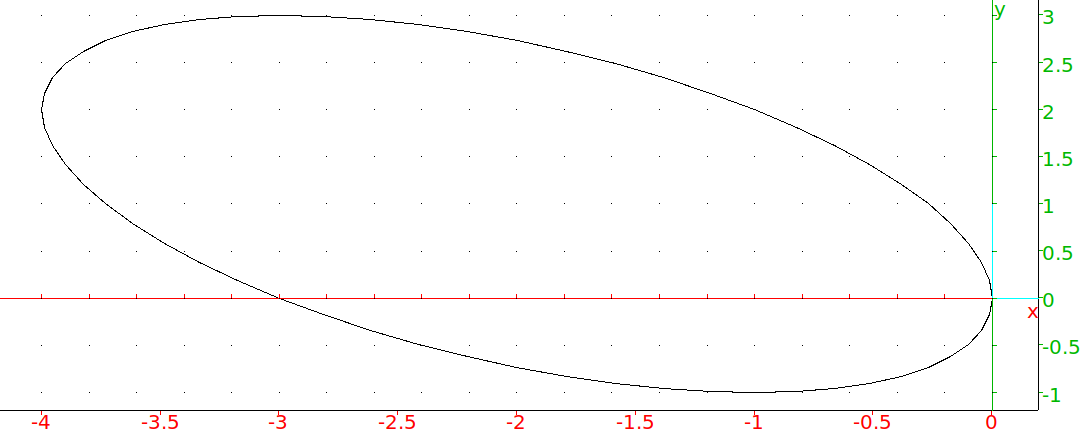
\includegraphics[width=0.75\textwidth]{xcas-conic1.png}
\end{center}
% Output:
% \begin{center}\texttt{the graph of the ellipsis of center -2+i and equation 2*x\^{}2+2*x*y+2*y\^{}2+6*x=0}\end{center}

\smallskip

See also the next section for the parametric equation of the conic.

\subsection{Conic reduction: \texttt{reduced\_conic}
\index{reduced\_conic}}

The \texttt{reduced\_conic} command finds the reduced equation of a
conic.
\begin{itemize}
  \item \texttt{reduced\_conic} takes two arguments:
  \begin{itemize}
    \item \textit{eq}, the equation of a conic.
    \item \textit{vars}, a list of the variable names.
  \end{itemize}
  \item \texttt{reduced\_conic(}\textit{eq,vars}\texttt{)}
  returns a list whose elements are:
  \begin{itemize}
  \item the origin of the conic,
  \item the matrix of a basis in which the conic is reduced,
  \item 0 or 1 (0 if the conic is degenerate),
  \item the reduced equation of the conic
  \item a vector of its parametric equations.
  \end{itemize}
\end{itemize}

\smallskip

\noindent
\textbf{Example.}\\
\textit{Input:}
\begin{center}
  \texttt{reduced\_conic(2*x\^{}2+2*x*y+2*y\^{}2+5*x+3,[x,y])}
\end{center}
\textit{Output:}
\begin{align*}
\Bigg[&\left[-\frac{5}{3},\frac{5}{6}\right],
      \left[\begin{array}{cc}\frac{\sqrt{2}}{2}&-\frac{\sqrt{2}}{2}\\
                         \frac{\sqrt{2}}{2}&\frac{\sqrt{2}}{2}\end{array}
      \right],1,3 x^{2}+y^{2}-\frac{7}{6},\\
      &\bigg[\frac{-10+5\mathrm{i}}{6}+\left(\frac{\sqrt{2}}{2}+\frac{1}{2} \mathrm{i}
      \sqrt{2}\right) \left(\frac{3}{18} \sqrt{14} \cos t+\frac{1}{6}
      \mathrm{i} \sqrt{42} \sin t\right),\\
      &t, 0, 2 \pi , \frac{2}{60}\pi , 2 x^{2}+2 x y+2 y^{2}+5 x+3,\\
      &\frac{-10+5
      \mathrm{i}}{6}+\frac{\left(\frac{\sqrt{2}}{2}+\frac{1}{2}
      \mathrm{i} \sqrt{2}\right) \left(\frac{3}{18} \sqrt{14}
      \left(1-t^{2}\right)+\frac{2}{6} \mathrm{i} \sqrt{42}
      t\right)}{1+t^{2}}\bigg]\Bigg]
\end{align*}
% \begin{center}
%   \texttt{[[-5/3,5/6],[[-1/(sqrt(2)),1/(sqrt(2))],[-1/(sqrt(2)), -1/(sqrt(2))]],1,3*x\^{}2+y\^{}2+-7/6,[[(-10+5*i)/6+ (1/(sqrt(2))+(i)/(sqrt(2)))*((sqrt(14)*cos(`~t`))/6+ ((i)*sqrt(42)*sin(` t`))/6),` t`,0,2*pi,(2*pi)/60]]]}
% \end{center}
Which means that the conic is not degenerate, its reduced equation is
\[
 3x^2+y^2-7/6=0 
\]
its origin is $-5/3+5*i/6$, its axes are
parallel to the vectors $(-1,1)$ and $(-1,-1)$, and its parametric equation is
\[ 
\frac{-10+5*i}{6}+ \frac{(1+i)}{\sqrt 2}*\frac{(\sqrt{14}*cos(t)+i*\sqrt{42}*sin(t))}{6}
\]
where the suggested parameter values for drawing are
$t$ from 0 to $2\pi$ with \texttt{tstep}= $2\pi/60$.

\smallskip

\noindent
\textbf{Remark}:\\ 
Note that if the conic is degenerate and is made of
1 or 2 line(s), the lines are not given by their parametric equation
but by the list of two points of the line.

\smallskip

\noindent
\textbf{Example.}\\
\textit{Input:}
\begin{center}
\texttt{reduced\_conic(x\^{}2-y\^{}2+3*x+y+2)}
\end{center}
\textit{Output:}
\[
\left[\left[-\frac{3}{2},\frac{1}{2}\right],\left[\begin{array}{cc}1&0\\0&1\end{array}\right],0,x^{2}-y^{2},\left[\begin{array}{cc}\frac{-3+\mathrm{i}}{2}&\frac{-1+3 \mathrm{i}}{2}\\\frac{-3+\mathrm{i}}{2}&\frac{-1-\mathrm{i}}{2}\end{array}\right]\right]
\]
%\begin{center}\texttt{[[(-3)/2,1/2],[[1,0],[0,1]],0,x\^{};2-y\^{}2, [[(-1+2*i)/(1-i),(1+2*i)/(1-i)], [(-1+2*i)/(1-i),(-1)/(1-i)]]]}\end{center}

\subsection{Graph of a quadric: \texttt{quadric}
\index{quadric}}

The \texttt{quadric} command draws a quadric.
\begin{itemize}
  \item \texttt{quadric} takes one mandatory argument and one optional
  argument:
  \begin{itemize}
    \item $q$, the expression of a quadric.
    \item Optionally, \textit{vars}, a list of three variable names
    (by default, $[x,y,z]$).  These names can also be given a separate
    arguments.
  \end{itemize}
  \item \texttt{quadric($q\,\langle$}\textit{vars}\texttt{$\rangle$)} draws this quadric.
\end{itemize}

\smallskip

\noindent
\textbf{Example.}\\
\textit{Input:}
\begin{center}
\texttt{quadric(7*x\^{}2+4*y\^{}2+4*z\^{}2+4*x*y-4*x*z-2*y*z-4*x+5*y+4*z-18)}
\end{center}
\textit{Output:}
\begin{center}
  Ellipsoid of center [0.407407407407,-0.962962962963,-0.537037037037]\\
  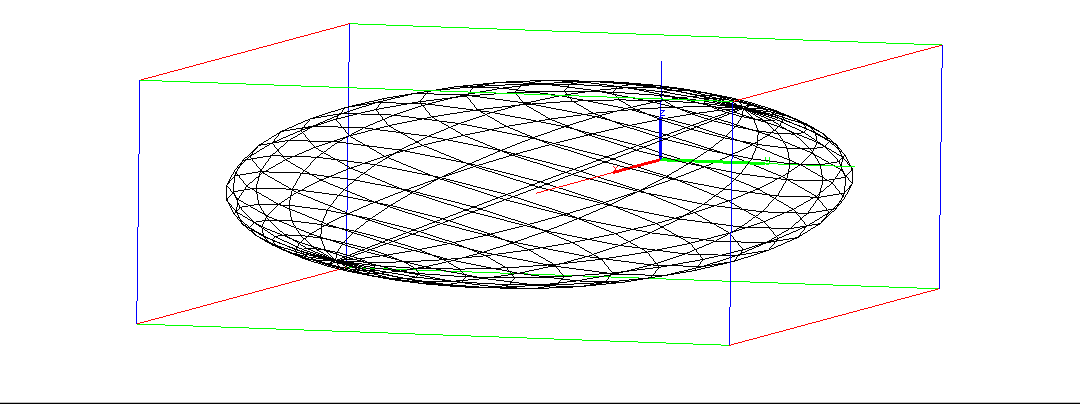
\includegraphics[width=0.75\textwidth]{xcas-quadric1.png}
\end{center}
%\begin{center}\texttt{the drawing of the ellipsoid of equation 7*x\^{}2+4*y\^{}2+4*z\^{}2+4*x*y-4*x*z-2*y*z-4*x+5*y+4*z-18=0}\end{center}

\smallskip

See also the next section for the parametric equation of the quadric.

\subsection{Quadric reduction: \texttt{reduced\_quadric}
\index{reduced\_quadric}}

The \texttt{reduced\_quadric} command finds the reduced equation of a
quadric.
\begin{itemize}
  \item \texttt{reduced\_quadric} takes two arguments:
  \begin{itemize}
    \item \textit{eq}, the equation of a quadric.
    \item \textit{vars}, a vector of variable names.
  \end{itemize}
  \item \texttt{reduced\_quadric(}\textit{eq,vars}\texttt{)} returns a
  list whose elements are: 
  \begin{itemize}
  \item the origin,
  \item the matrix of a basis where the quadric is reduced,
  \item 0 or 1 (0 if the quadric is degenerate),
  \item the reduced equation of the quadric
  \item a vector with its parametric equations.
  \end{itemize}
\end{itemize}
\textbf{Warning !}
\texttt{u,v} will be used as parameters of the parametric equations:
these variables should not be assigned (\texttt{purge} them before
calling \texttt{reduced\_quadric}).

\smallskip

\noindent
\textbf{Example.}\\
\textit{Input:}
\begin{center}
\texttt{reduced\_quadric(7*x\^{}2+4*y\^{}2+4*z\^{}2+ 4*x*y-4*x*z-2*y*z-4*x+5*y+4*z-18)}
\end{center}
\textit{Output:}
\begin{align*}
\Bigg[&
   \left[\frac{11}{27},-\frac{26}{27},-\frac{29}{54}\right],
   \left[\begin{array}{ccc}\frac{\sqrt{6}}{3}&\frac{\sqrt{5}}{5}&-\frac{\sqrt{30}}{15}\\\frac{\sqrt{6}}{6}&0&\frac{\sqrt{30}}{6}\\-\frac{\sqrt{6}}{6}&\frac{2}{5}
        \sqrt{5}&\frac{\sqrt{30}}{30}\end{array}\right],
   \left[9,3,3\right],1,9 x^{2}+3 y^{2}+3 z^{2}-\frac{602}{27},\\
   &\Bigg[\bigg[
        \frac{9 \sqrt{6} \sqrt{1806} \sin u\cdot \cos v}{3\cdot
        243}+\frac{9 \sqrt{5} \sqrt{602} \sin u\cdot \sin v}{5\cdot
        81}-\frac{9 \sqrt{30} \sqrt{602} \cos u}{15\cdot 81}+\frac{11}{27},\\
        &\quad\frac{9 \sqrt{6} \sqrt{1806} \sin u\cdot \cos v}{6\cdot
        243}+\frac{9 \sqrt{30} \sqrt{602} \cos u}{6\cdot
        81}-\frac{26}{27},\\
        &\quad-\frac{9 \sqrt{6} \sqrt{1806} \sin u\cdot \cos v}{6\cdot 243}+\frac{9\cdot 2 \sqrt{5} \sqrt{602} \sin u\cdot \sin v}{5\cdot 81}+\frac{9 \sqrt{30} \sqrt{602} \cos u}{30\cdot 81}-\frac{29}{54}
        \bigg],\\
           &\qquad u=0\ldots \pi ,v=0\ldots 2 \pi ,\mathrm{ustep}=\frac{\pi
           }{20},\mathrm{vstep}=\frac{2}{20} \pi 
    \Bigg]\Bigg]
\end{align*}
The output is a list containing:
\begin{itemize}
\item The origin (center of symmetry) of the quadric
\[
\left[\frac{11}{27},-\frac{26}{27},-\frac{29}{54}\right]
\]
%\begin{center}\texttt{[11/27,(-26)/27,(-29)/54],}\end{center}
\item The matrix of the basis change:
\[
\left[\begin{array}{ccc}\frac{\sqrt{6}}{3}&\frac{\sqrt{5}}{5}&-\frac{\sqrt{30}}{15}\\\frac{\sqrt{6}}{6}&0&\frac{\sqrt{30}}{6}\\-\frac{\sqrt{6}}{6}&\frac{2}{5}
        \sqrt{5}&\frac{\sqrt{30}}{30}\end{array}\right],
\]
% \begin{center}\texttt{[[(sqrt(6))/3,(sqrt(5))/5,(-(sqrt(30)))/15],
%     [(sqrt(6))/6,0,(sqrt(30))/6],
%     [(-(sqrt(6)))/6,(2*sqrt(5))/5,(sqrt(30))/30]],}\end{center}
\item 1, hence the quadric is not degenerated
\item the reduced equation of the quadric:
\[
9 x^{2}+3 y^{2}+3 z^{2}-\frac{602}{27}
\]
%\begin{center}{\texttt{0,9*x\^{}2+3*y\^{}2+3*z\^{}2+(-602)/27,}}\end{center}
\item
The parametric equations (in the original frame):
\begin{align*}
\Bigg[&\bigg[
     \frac{9 \sqrt{6} \sqrt{1806} \sin u\cdot \cos v}{3\cdot
     243}+\frac{9 \sqrt{5} \sqrt{602} \sin u\cdot \sin v}{5\cdot
     81}-\frac{9 \sqrt{30} \sqrt{602} \cos u}{15\cdot 81}+\frac{11}{27},\\
     &\quad\frac{9 \sqrt{6} \sqrt{1806} \sin u\cdot \cos v}{6\cdot
     243}+\frac{9 \sqrt{30} \sqrt{602} \cos u}{6\cdot
     81}-\frac{26}{27},\\
     &\quad-\frac{9 \sqrt{6} \sqrt{1806} \sin u\cdot \cos v}{6\cdot 243}+\frac{9\cdot 2 \sqrt{5} \sqrt{602} \sin u\cdot \sin v}{5\cdot 81}+\frac{9 \sqrt{30} \sqrt{602} \cos u}{30\cdot 81}-\frac{29}{54}
     \bigg],\\
       &\qquad u=0\ldots \pi ,v=0\ldots 2 \pi ,\mathrm{ustep}=\frac{\pi
       }{20},\mathrm{vstep}=\frac{2}{20} \pi 
 \Bigg]
\end{align*}
% \begin{center}\texttt{[[(sqrt(6)*sqrt(602/243)*sin(u)*cos(v))/3+
%     (sqrt(5)*sqrt(602/81)*sin(u)*sin(v))/5+
%     ((-(sqrt(30)))*sqrt(602/81)*cos(u))/15+11/27,
%     (sqrt(6)*sqrt(602/243)*sin(u)*cos(v))/6+
%     (sqrt(30)*sqrt(602/81)*cos(u))/6+(-26)/27,
%     ((-(sqrt(6)))*sqrt(602/243)*sin(u)*cos(v))/6+
%     (2*sqrt(5)*sqrt(602/81)*sin(u)*sin(v))/5+
%     (sqrt(30)*sqrt(602/81)*cos(u))/30+(-29)/54],
%      u=(0 .. pi),v=(0.. (2*pi)),ustep=(pi/20),
%      vstep=((2*pi)/20)]]}\end{center}
\end{itemize}
Hence the quadric is an ellipsoid and its reduced equation is:
\[ 
9x^2+3y^2+3z^2+(-602)/27 = 0
\]
after the change of origin $[11/27,(-26)/27,(-29)/54]$,
the matrix of basis change is:
\[ 
\left[
\begin{array}{ccc}
\displaystyle \frac{\sqrt 6}{3} & \displaystyle\frac{\sqrt 5}{5} & \displaystyle-\frac{\sqrt{30}}{15}\\
\displaystyle \frac{\sqrt 6}{6} & 0 & \displaystyle \frac{\sqrt{30}}{6}\\
\displaystyle -\frac{\sqrt 6}{6} & \displaystyle \frac{2\sqrt{5}}{5} & \displaystyle \frac{\sqrt{30}}{30}\\
\end{array}
\right] 
\]
Its parametric equation is:
\[ 
\left\{
\begin{array}{l}
x =\displaystyle \frac{\sqrt 6\sqrt{\frac{602}{243}}\sin(u)\cos(v)}{3}+\frac{\sqrt 5\sqrt{\frac{602}{81}}\sin(u)\sin(v)}{5}-\frac{\sqrt{30}\sqrt{\frac{602}{81}}\cos(u)}{15}+\frac{11}{27}\\
y =\displaystyle \frac{\sqrt 6\sqrt{\frac{602}{243}}\sin(u)\cos(v)}{6}+\frac{\sqrt{30}\sqrt{\frac{602}{81}}\cos(u))}{6}-\frac{26}{27}\\
z =\displaystyle \frac{-\sqrt 6\sqrt{\frac{602}{243}}*\sin(u)\cos(v)}{6}+\frac{2\sqrt 5\sqrt{\frac{602}{81}}\sin(u)\sin(v)}{5}+\frac{\sqrt{30}\sqrt{\frac{602}{81}}\cos(u)}{30}-\frac{29}{54}
\end{array}
\right.
\]

\smallskip

\noindent
\textbf{Remark}:\\
Note that if the quadric is degenerate and made of 1 or 2 plane(s),
each plane is not given by
its parametric equation but by the list of a point of the plane
and of a normal vector to the plane.

\smallskip

\noindent
\textbf{Example.}\\
\textit{Input:}
\begin{center}
\texttt{reduced\_quadric(x\^{}2-y\^{}2+3*x+y+2)}
\end{center}
\textit{Output:}
\begin{align*}
\Bigg[&\left[-\frac{3}{2},\frac{1}{2},0\right],\left[\begin{array}{ccc}1&0&0\\0&1&0\\0&0&-1\end{array}\right],\\
&\left[0,1,-1\right],x^{2}-y^{2},\\
&\left[\mathrm{hyperplan}\left(\left[1,1,0\right],\left[-\frac{3}{2},\frac{1}{2},0\right]\right),\mathrm{hyperplan}\left(\left[1,-1,0\right],\left[-\frac{3}{2},\frac{1}{2},0\right]\right)\right]\Bigg]
\end{align*}
%\begin{center}\texttt{[[(-3)/2,1/2,0],[[1,0,0],[0,1,0],[0,0,-1]],0,x\^{}2-y\^{}2, [hyperplan([1,1,0],[(-3)/2,1/2,0]), hyperplan([1,-1,0],[(-3)/2,1/2,0])]]}\end{center}
              
\section{Equations}

\subsection{Defining an equation: \texttt{equal}
\index{equal}}

The \texttt{equal} command creates equations; it is the infixed
version of \texttt{=}.
\begin{itemize}
  \item \texttt{equal} takes two arguments:\\
  \textit{lhs} and \textit{rhs}, the two sides of the equation.
  \item \texttt{equal(}\textit{lhs,rhs}\texttt{)} returns the equation 
  \textit{lhs$=$rhs}.
\end{itemize}

\smallskip

\noindent
\textbf{Example.}\\
\textit{Input:}
\begin{center}
\texttt{equal(2x-1,3)}
\end{center}
\textit{Output:}
\[
2 x-1=3
\]
%\begin{center}\texttt{(2*x-1)=3}\end{center}
You can also directly write \texttt{(2*x-1)=3}.

\subsection{Transforming an equation into a difference: \texttt{equal2diff}
\index{equal2diff}}

The \texttt{equal2diff} command turns an equation into the difference
of the two sides, resulting in an expression assumed to be equal to 0.
\begin{itemize}
  \item \texttt{equal2diff} takes one argument:\\
  \textit{lhs$=$rhs},  an equation.
  \item \texttt{equal2diff(}\textit{lhs$=$rhs}\texttt{)} returns the
  difference \textit{lhs $-$ rhs}.
\end{itemize}

\smallskip

\noindent
\textbf{Example.}\\
\textit{Input:}
\begin{center}
\texttt{equal2diff(2x-1=3)}
\end{center}
\textit{Output:}
\[
2 x-1-3
\]
%\begin{center}\texttt{2*x-1-3}\end{center}

\subsection{Transforming an equation into a list: \texttt{equal2list}
\index{equal2list}}

The \texttt{equal2list} command separates the two sides of an equation.
\begin{itemize}
  \item \texttt{equal2list} takes one argument:\\
  \textit{lhs$=$rhs}, an equation.
  \item \texttt{equal2list(}\textit{lhs$=$rhs}\texttt{)} returns the
  sequence \textit{lhs,rhs}.
\end{itemize}


\smallskip

\noindent
\textbf{Example.}\\
\textit{Input:}
\begin{center}
\texttt{equal2list(2x-1=3)}
\end{center}
\textit{Output:}
\[
2 x-1,3
\]

\subsection{The left member of an equation: \texttt{left} \texttt{gauche} \texttt{lhs}
\index{left|textbf}
\index{lhs|textbf}
\index{gauche|textbf}
\label{ssec:lhs}}

(See \secref{ssec:lrstring}, \secref{ssec:op}, \secref{ssec:range}, \secref{ssec:lrinterval},
\secref{ssec:lrlist} and \secref{ssec:rhs} for
other uses of \texttt{left} and \texttt{right}.)

The \texttt{left} command finds the left hand side of an equation.\\
For this, \texttt{lhs} is a synonym for \texttt{left}.
\begin{itemize}
  \item \texttt{left} takes one argument:\\
  \textit{lhs$=$rhs}, an equation.
  \item \texttt{left(}\textit{lhs$=$rhs}\texttt{)} returns \textit{lhs}.
\end{itemize}

\smallskip

\noindent
\textbf{Example.}\\
\textit{Input:}
\begin{center}
\texttt{left(2x-1=3)}
\end{center}
\textit{or:}
\begin{center}
\texttt{lhs(2x-1=3)}
\end{center}
\textit{Output:}
\[
2 x-1
\]
%\begin{center}\texttt{2*x-1}\end{center}

\subsection{The right member of an equation: \texttt{right} \texttt{droit} \texttt{rhs}
\index{right|textbf}
\index{rhs|textbf}
\index{droit|textbf}
\label{ssec:rhs}}

(See \secref{ssec:lrstring}, \secref{ssec:op}, \secref{ssec:range}, \secref{ssec:lrinterval},
\secref{ssec:lrlist} and \secref{ssec:lhs} for
other uses of \texttt{left} and \texttt{right}.)

The \texttt{right} command finds the right hand side of an equation.\\
For this, \texttt{rhs} is a synonym for \texttt{right}.
\begin{itemize}
  \item \texttt{right} takes one argument:\\
  \textit{lhs$=$rhs}, an equation.
  \item \texttt{right(}\textit{lhs$=$rhs}\texttt{)} returns \textit{rhs}.
\end{itemize}

\smallskip

\noindent
\textbf{Example.}\\
\textit{Input:}
\begin{center}
\texttt{right(2x-1=3)}
\end{center}
\textit{or:}
\begin{center}
\texttt{rhs(2x-1=3)}
\end{center}
\textit{Output:}
\[
3
\]
%\begin{center}\texttt{2*x-1}\end{center}

\subsection{Solving equation(s): \texttt{solve} \texttt{cSolve}
\index{solve|textbf}
\index{cSolve|textbf}
\label{ssec:solve}}

The \texttt{solve} command solves an equation or a system of
polynomial equations.   In real mode, \texttt{solve} returns only real
solutions; to have \texttt{solve} return the complex solutions, switch
to complex mode (e.g.by checking \texttt{Complex} in the cas
configuration, see \secref{ssec:complex}).

The \texttt{cSolve} command is identical to \texttt{solve}, except it
returns the complex solutions whether in real mode or complex mode.

To solve an equation:
\begin{itemize}
  \item \texttt{solve} takes one mandatory argument and one optional
  argument:
  \begin{itemize}
    \item \textit{eqn}, an equation or expression assumed to be zero.
    \item Optionally, $x$, a variable (by default, $x$\texttt{=x}).
  \end{itemize}
  \item \texttt{solve(}\textit{eqn}\texttt{,$x$)} returns the solution
  to the equation.
\end{itemize}
For trigonometric equations, \texttt{solve} returns by default the principal
solutions. To have all the solutions check \texttt{All\_trig\_sol} in the cas
configuration (see \secref{ssec:confcomp}, item \ref{enum:trig}).

\textbf{Examples}:
\begin{itemize}
\item 
Solve $x^4-1=3$\\
\textit{Input:}
\begin{center}
\texttt{solve(x\^{}4-1=3)}
\end{center}
\textit{Output (in real mode):}
\[
\left[\sqrt{2},-\sqrt{2}\right]
\]
% \begin{center}
% \texttt{[sqrt(2),-(sqrt(2))]}
% \end{center}
\textit{Output (in complex mode):}
\[
\left[\sqrt{2},-\sqrt{2},\mathrm{i}\sqrt{2},-\mathrm{i}\sqrt{2}\right]
\]
%\begin{center}\texttt{[sqrt(2),-(sqrt(2)),(i)*sqrt(2),-((i)*sqrt(2))]}\end{center}
Also:\\
\textit{Input:}
\begin{center}
\texttt{cSolve(x\^{}4-1=3)}
\end{center}
\textit{Output (in any mode):}
\[
\left[-\sqrt{2},\sqrt{2},-\sqrt{2} \mathrm{i},\sqrt{2} \mathrm{i}\right]
\]
\item 
Solve $\exp(x)=2$\\
\textit{Input:}
\begin{center}
\texttt{solve(exp(x)=2)}
\end{center}
\textit{Output:}
\[
\left[\ln \left(2\right)\right]
\]
%\begin{center}\texttt{[log(2)]}\end{center}
\item 
Solve $\cos(2*x)=1/2$\\
\textit{Input:}
\begin{center}
\texttt{solve(cos(2*x)=1/2)}
\end{center}
\textit{Output:}
\[
\left[-\frac{\pi }{6},\frac{\pi }{6}\right]
\]
%\begin{center}\texttt{[pi/6,(-pi)/6]}\end{center}
\textit{Output (with \texttt{All\_trig\_sol} checked):}
\[
\left[\frac{6\pi n_0 + \pi}{6},\frac{6\pi n_0 - \pi }{6}\right]
\]
%\begin{center}\texttt{[(6*pi*n\_0+pi)/6,(6*pi*n\_0-pi)/6]}\end{center}
\end{itemize}

\smallskip

To solve a system of polynomial equations:
\begin{itemize}
  \item \texttt{solve} takes one mandatory argument and one optional
  argument:
  \begin{itemize}
    \item \textit{eqns}, a list of polynomial equations.
    \item \textit{vars}, a list of variables.
  \end{itemize}
  \item \texttt{solve(}\textit{eqns,vars}\texttt{)} returns the
  solutions to the system of equations.
\end{itemize}


\smallskip

\noindent
\textbf{Examples.}
\begin{itemize}
\item Find $x,y$ such that $x+y=1,x-y=0$\\
\textit{Input:}
\begin{center}
\texttt{solve([x+y=1,x-y],[x,y])}
\end{center}
\textit{Output:}
\[
\left[\left[\frac{1}{2},\frac{1}{2}\right]\right]
\]
%\begin{center}\texttt{[[1/2,1/2]]}\end{center}
\item Find $x,y$ such that $x^2+y=2,x+y^2=2$\\
\textit{Input:}
\begin{center}
\texttt{solve([x\^{}2+y=2,x+y\^{}2=2],[x,y])}
\end{center}
\textit{Output:}
\[
\left[\left[1,1\right],\left[-2,-2\right],\left[\frac{\sqrt{5}+1}{2},-\left(\frac{\sqrt{5}+1}{2}\right)^{2}+2\right],\left[\frac{-\sqrt{5}+1}{2},-\left(\frac{-\sqrt{5}+1}{2}\right)^{2}+2\right]\right]
\]
%\begin{center}\texttt{[[-2,-2],[1,1],[(-sqrt(5)+1)/2,(1+sqrt(5))/2],}\end{center}
\begin{center}\texttt{[(sqrt(5)+1)/2,(1-sqrt(5))/2]]}\end{center}
\item 
Find $x,y,z$ such that $x^2-y^2=0,x^2-z^2=0$\\
\textit{Input:}
\begin{center}
\texttt{solve([x\^{}2-y\^{}2=0,x\^{}2-z\^{}2=0],[x,y,z])}
\end{center}
\textit{Output:}
\[
\left[\left[x,x,x\right],\left[x,-x,-x\right],\left[x,x,-x\right],\left[x,-x,x\right]\right]
\]
%\begin{center}\texttt{[[x,x,x],[x,-x,-x],[x,-x,x],[x,x,-x]]}\end{center}
\item
Find the intersection of a straight line
(given by a list of equations) and a plane.\\ 
For example, let $D$ be the straight line with cartesian equations
$[y-z=0,z-x=0]$ and let $P$ the plane with equation $x-1+y+z=0$.
Find the intersection of $D$ and $P$.\\
\textit{Input:}
\begin{center}
\texttt{solve([[y-z=0,z-x=0],x-1+y+z=0],[x,y,z])}
\end{center}
\textit{Output:}
\[
\left[\left[\frac{1}{3},\frac{1}{3},\frac{1}{3}\right]\right]
\]
%\begin{center}\texttt{[[1/3,1/3,1/3]]}\end{center}
\item
\textit{Input:}
\begin{center}
\texttt{cSolve([-x\^{}2+y=2,x\^{}2+y],[x,y])}
\end{center}
\textit{Output:}
\[
\left[\left[-\mathrm{i},1\right],\left[\mathrm{i},1\right]\right]
\]
%\begin{center}\texttt{[[i,1],[-i,1]]}\end{center}
\end{itemize}

\section{Linear systems}

The \emph{augmented matrix} of the system $A \cdot X=b$ is either the 
matrix obtained by gluing the column vector $b$ to the right
of the matrix $A$ (as with \texttt{border($A$,tran($b$))}), 
representing $A \cdot X=b$, or the
matrix obtained by gluing the column vector $-b$ to the right of the
matrix $A$, representing $A\cdot x - b = 0$.

\subsection{Matrix of a system: \texttt{syst2mat}
\index{syst2mat}}

The \texttt{syst2mat} command turns a system of linear equations into
its augmented matrix.  (For this command, the augmented matrix of
$Ax=b$ has the column vector $-b$ glued to the right of $A$.)
\begin{itemize}
  \item \texttt{syst2mat} takes two as arguments:
  \begin{itemize}
    \item \textit{eqns}, a list of the equations or expressions
    (assumed to be equal to zero) of a linear system.
    \item \textit{vars}, a list of the variable names.
  \end{itemize}
  \item \texttt{syst2mat(}\textit{eqns,vars}\texttt{)} returns the
  augmented matrix of the system.
\end{itemize}
\textbf{Warning !!!}\\
The variables must be purged before \texttt{syst2mat} is called.

\smallskip

\noindent
\textbf{Examples.}
\begin{itemize}
\item 
\textit{Input:}
\begin{center}
\texttt{syst2mat([x+y,x-y-2],[x,y])}
\end{center}
\textit{Output:}
\[
\begin{pmatrix}1&1&0\\1&-1&-2\end{pmatrix}
\]
%\begin{center}\texttt{[[1,1,0],[1,-1,-2]]}\end{center}
\item
\textit{Input:}
\begin{center}
\texttt{syst2mat([x+y=0,x-y=2],[x,y])}
\end{center}
\textit{Output:}
\[
\begin{pmatrix}1&1&0\\1&-1&-2\end{pmatrix}
\]
%\begin{center}\texttt{[[1,1,0],[1,-1,-2]]}\end{center}
\end{itemize}

\subsection{Gauss reduction of a matrix: \texttt{ref}
\label{ssec:ref}
\index{ref}}

A matrix $A$ is in row-echelon form if the first non-zero element of
each row is 1 and each of these leading 1s is further right than the
leading 1s of the preceding rows.  Gaussian elimination will transform
a matrix into row echelon form, and the row echelon form of the
augmented matrix of a system of linear equations has the same set of
solutions as the original, but in a form that is simple to solve.

The \texttt{ref} command transforms a matrix into a row echelon form
of the matrix.
\begin{itemize}
  \item \texttt{ref} takes one argument:\\
  $A$, a matrix.
  \item \texttt{ref($A$)} returns a row echelon form of a matrix.
\end{itemize}
\texttt{ref} is typically used to solve a linear system of equations
written in matrix form.

\smallskip

\noindent
\textbf{Example.}\\
Solve the system: 
\[ 
\left\{
   \begin{array}{lcr} 
     3x + y & = &-2 \\
     3x +2y & =& 2 
   \end{array}\right.
\]
\textit{Input:}
\begin{center}
\texttt{ref([[3,1,-2],[3,2,2]])}
\end{center}
\textit{Output:}
\[
\left[\begin{array}{ccc}1&\frac{1}{3}&-\frac{2}{3}\\0&1&4\end{array}\right]
%\left[\begin{array}{ccc}1&\frac{1}{3}&-\frac{2}{3}\\0&1&4\end{array}\right]
\]
%\begin{center}\texttt{[[1,1/3,-2/3],[0,1,4]]}\end{center}
Hence the solution is $y=4$ (from the last row) and $x=-2$
(substitute $y$ in the first row).

\subsection{Gauss-Jordan reduction: \texttt{rref} \texttt{gaussjord}\label{ssec:rref}
\index{rref|textbf}
\index{gaussjord|textbf}}

The reduced row echelon form of a matrix is the row echelon form (see
previous section) with 0s above the leading 1s in each row.
Gauss-Jordan reduction will turn any matrix into reduced row echelon
form, and the reduced row echelon form of a matrix is unique.  If the
matrix is the augmented matrix of a system, then the reduced row
echelon form of the matrix is the simplest form to solve the system.
The \texttt{rref} command finds the reduced row echelon form of a
matrix (see also \secref{ssec:rrefm}).
\begin{itemize}
  \item \texttt{rref} takes one mandatory and one optional argument:
  \begin{itemize}
    \item $A$, a matrix.
    \item Optionally, $n$, a positive integer.
  \end{itemize}
  \item \texttt{rref($A\,\langle n\rangle$)} returns the reduced row
  echelon form of the matrix.  With a second argument of $n$,
  Gauss-Jordan reduction will be performed on (at most) the first $n$
  columns.
\end{itemize}

\smallskip

\noindent
\textbf{Examples.}
\begin{itemize}
\item 
Solve the system:
\[
\left 
\{
\begin{array}{lcr} 
3x + y & = &-2 \\
3x +2y & =& 2 
\end{array}\right.
\]
\textit{Input:}
\begin{center}
\texttt{rref([[3,1,-2],[3,2,2]])}
\end{center}
\textit{Output:}
\[
\left[\begin{array}{ccc}1&0&-2\\0&1&4\end{array}\right]
\]
%\begin{center}\texttt{[[1,0,-2],[0,1,4]]}\end{center}
Hence $x=-2$ and $y=4$ is the solution of this system.
\item
\texttt{rref} can also solve several linear systems of
equations having the same matrix of coefficients by augmenting the
matrix of coefficients by vectors representing the right hand side of
the equations for each equation.  For example,
Solve the systems:
\[
\left \{
\begin{array}{lcr} 
  3x + y & = &-2 \\
  3x +2y & =& 2 
\end{array}\right.
\]
and 
\[
\left \{
\begin{array}{lcr} 
3x + y & = &1 \\
3x +2y & =& 2 
\end{array}\right.
\]
\textit{Input:}
\begin{center}
\texttt{rref([[3,1,-2,1],[3,2,2,2]])}
\end{center}
\textit{Output:}
\[
\left[\begin{array}{cccc}1&0&-2&0\\0&1&4&1\end{array}\right]
\]
%\begin{center}\texttt{[[1,0,-2,0],[0,1,4,1]]}\end{center}
Which means that $x=-2$ and $y=4$ is the solution of the first system
and $x=0$ and $y=1$ is the solution of the second system.
\item
\textit{Input:}
\begin{center}
\texttt{rref([[3,1,-2,1],[3,2,2,2]],1)}
\end{center}
\textit{Output:}
\[
\left[\begin{array}{cccc}1&\frac{1}{3}&-\frac{2}{3}&\frac{1}{3}\\0&3&12&3\end{array}\right]
\]
%\begin{center}\texttt{[[3,1,-2,1],[0,1,4,1]]}\end{center}
and Gauss-Jordan reduction has been performed only on the first column.
\end{itemize}

\subsection{Solving $AX=b$: \texttt{simult}
\index{simult}}

The \texttt{simult} command can  solve a linear system of equations or 
several linear systems of equations with the same matrix of
coefficients (see also \ref{ssec:rref}).
\begin{itemize}
  \item \texttt{simult} takes two arguments:
  \begin{itemize}
    \item $A$, a matrix (the matrix of coefficients of a system).
    \item $b$, a column vector (representing the right hand side of
    the system) or a matrix (where each column represents the right
    hand side of an equation).
  \end{itemize}
  \item \texttt{simult($A,b$)} returns a column vector of the
  solutions (or a matrix where each column is the column vector of a
  solution).
\end{itemize}

\smallskip

\noindent
\textbf{Examples.}
\begin{itemize}
\item Solve
\[
\left\{
\begin{array}{lcr} 
  3x + y & = &-2 \\
  3x +2y & =& 2 
\end{array}\right.
\]
\textit{Input:}
\begin{center}
\texttt{simult([[3,1],[3,2]],[[-2],[2]])}
\end{center}
\textit{Output:}
\[
\left[\begin{array}{c}-2\\4\end{array}\right]
\]
\begin{center}\texttt{[[-2],[4]]}\end{center}
Hence $x=-2$ and $y=4$ is the solution.
\item
Solve
\[
\left\{
\begin{array}{lcr} 
3x + y & = &-2 \\3
x +2y & =& 2 
\end{array}\right.
\]
and
\[
\left\{
\begin{array}{lcr} 
3x + y & = &1 \\
3x +2y & =& 2 
\end{array}\right.
\]
\textit{Input:}
\begin{center}
\texttt{simult([[3,1],[3,2]],[[-2,1],[2,2]])}
\end{center}
\textit{Output:}
\[
\left[\begin{array}{cc}-2&0\\4&1\end{array}\right]
\]
So $x=-2$ and $y=4$ is the solution of the first system of equations
and $x=0$ and $y=1$ is the solution of the second system.
%\begin{center}\texttt{[[-2,0],[4,1]]}\end{center}
\end{itemize}

\subsection{Step by step Gauss-Jordan reduction of a matrix: \texttt{pivot}\label{ssec:pivot}
\index{pivot}}

One step of Gauss-Jordan elimination involves taking a non-zero
element of a matrix (the pivot) and adding multiples of its row to the
other rows to get zeros above and below the pivot.  The \texttt{pivot}
command performs this operation.
\begin{itemize}
  \item \texttt{pivot} takes three arguments:
  \begin{itemize}
    \item $A$, a a matrix with $n$ rows and $p$ columns.
    \item $l$ and $c$, two integers such that $l$ is the index of a
    row of $A$ and $c$ is an index of column of $A$, and the element
    of $A$ in row $l$ and column $c$ is non-zero.
  \end{itemize}
  \item \texttt{pivot($A,l,c$)} returns the result of performing one
  step of the Gauss-Jordan method using the element of $A$ in row $l$,
  column $c$ as pivot.
\end{itemize}

\smallskip

\noindent
\textbf{Examples.}
\begin{itemize}
\item 
\textit{Input:}
\begin{center}
\texttt{pivot([[1,2],[3,4],[5,6]],1,1)}
\end{center}
\textit{Output:}
\[
\left[\begin{array}{cc}-2&0\\3&4\\2&0\end{array}\right]
\]
%\begin{center}\texttt{[[-2,0],[3,4],[2,0]]}\end{center}
\item
\textit{Input:}
\begin{center}
\texttt{pivot([[1,2],[3,4],[5,6]],0,1)}
\end{center}
\textit{Output:}
\[
\left[\begin{array}{cc}1&2\\2&0\\4&0\end{array}\right]
\]
%\begin{center}\texttt{[[1,2],[2,0],[4,0]]}\end{center}
\end{itemize}

\subsection{Linear system solving: \texttt{linsolve}
\index{linsolve}}

The \texttt{linsolve} command solves systems of linear equations.
It can take its arguments as a list of equations or as a matrix of
coefficients followed by a vector of the right hand side.  It can also
take the matrix of coefficients after an LU factorization (see
\secref{ssec:lu}), which  can be useful when you have several systems
of equations which only differ on their right hand side.  
If the \texttt{Step by step} box is 
is checked in the general configuration (see \secref{sec:mconf}), 
\texttt{linsolve} will show you the steps in
getting a solution.

Given a system of equations:
\begin{itemize}
  \item \texttt{linsolve} takes two arguments:
  \begin{itemize}
    \item \textit{eqns}, a list of linear equations or expressions
    (where each expression is assumed to be equal to zero).
    \item \textit{vars}, a list of variable names.
  \end{itemize}
  \item \texttt{linsolve(}\textit{eqns,vars}\texttt{)} returns the
  solution of the equations as a list.
\end{itemize}

\smallskip

\noindent
\textbf{Examples.}
\begin{itemize}
\item 
\textit{Input:}
\begin{center}
\texttt{linsolve([2*x+y+z=1,x+y+2*z=1,x+2*y+z=4],[x,y,z])}
\end{center}
\textit{Output:}
\[
\left[-\frac{1}{2},\frac{5}{2},-\frac{1}{2}\right]
\]
%\begin{center}\texttt{[1/-2,5/2,1/-2]}\end{center}
Which means that
\[ x=-\frac{1}{2}, y=\frac{5}{2}, z=-\frac{1}{2} \]
is the solution of the system:
\[
\left\{
\begin{array}{rl}
2x+y+z &=1\\
x+y+2z &=1\\
x+2y+z &=4
\end{array}
\right.
\]
\item
\textit{Input:}
\begin{center}
\texttt{linsolve([x+2*y+3*z=1,3*x+2*y+z=2],[x,y,z])}
\end{center}
\textit{Output:}
\[
\left[z+\frac{1}{2},-2 z+\frac{1}{4},z\right]
\]
\end{itemize}

\smallskip

Given the matrix of coefficients:
\begin{itemize}
  \item  \texttt{linsolve} takes two arguments:
  \begin{itemize}
    \item $A$, the matrix of coefficients of a linear system.
    \item $b$, a list of the values of the right hand side of the
    system.
  \end{itemize}
  \item \texttt{linsolve($A,b$)} returns the solution of the
  corresponding equations as a list.
\end{itemize}

\smallskip

\noindent
\textbf{Example.}\\
\textit{Input:}
\begin{center}
  \texttt{linsolve ([[2,1,1], [1,1,2], [1,2,1]], [1,1,4])}
\end{center}
\textit{Output:}
\[
\left[-\frac{1}{2},\frac{5}{2},-\frac{1}{2}\right]
\]
% \begin{center}
%   \texttt{[-1/2,5/2,-1/2]}
% \end{center}
If the \texttt{Step by step} option is checked in the general
configuration, a window will also pop up showing:
\begin{align*}
%[[2,1,1,-1],[1,1,2,-1],[1,2,1,-4]]
&\left[\begin{array}{cccc}2&1&1&-1\\1&1&2&-1\\1&2&1&-4\end{array}\right]\\
&\text{Reduce column 1 with pivot 1 at row 2}\\
&\text{Exchange row 1 and row 2}\\
&L_2 <-(1)*L_2 -(2)*L_1 \text{ on } \left[\begin{array}{cccc}1&1&2&-1\\2&1&1&-1\\1&2&1&-4\end{array}\right]\\
%[[1,1,2,-1],[2,1,1,-1],[1,2,1,-4]]
&L_3 <- 1*L_3 -(1)*L_1 \text{ on } \left[\begin{array}{cccc}1&1&2&-1\\0&-1&-3&1\\1&2&1&-4\end{array}\right]\\
%[[1,1,2,-1],[0,-1,-3,1],[1,2,1,-4]]
&\left[\begin{array}{cccc}1&1&2&-1\\0&-1&-3&1\\0&1&-1&-3\end{array}\right]\\
%[[1,1,2,-1],[0,-1,-3,1],[0,1,-1,-3]]
&\text{Reduce column 2 with pivot 1 at row 3}\\
&\text{Exchange row 2 and row 3}\\
&L_1 <- (1)*L_1-(1)*L_2 on \left[\begin{array}{cccc}1&1&2&-1\\0&1&-1&-3\\0&-1&-3&1\end{array}\right]\\
%[[1,1,2,-1],[0,1,-1,-3],[0,-1,-3,1]]
&L_3 <- (1)*L_3-(-1)*L_2 \text{ on } \left[\begin{array}{cccc}1&0&3&2\\0&1&-1&-3\\0&-1&-3&1\end{array}\right]\\
%[[1,0,3,2],[0,1,-1,-3],[0,-1,-3,1]]
&\left[\begin{array}{cccc}1&0&3&2\\0&1&-1&-3\\0&0&-4&-2\end{array}\right]\\
%[[1,0,3,2],[0,1,-1,-3],[0,0,-4,-2]]
&\text{Reduce column 3 with pivot -4 at row 3}\\
&L_1 <- (1)*L_1-(-3/4)*L_3 \text{ on } \left[\begin{array}{cccc}1&0&3&2\\0&1&-1&-3\\0&0&-4&-2\end{array}\right]\\
%[[1,0,3,2],[0,1,-1,-3],[0,0,-4,-2]]
&L_2 <- (1)*L_2-(1/4)*L_3 \text{ on } \left[\begin{array}{cccc}1&0&0&\frac{1}{2}\\0&1&-1&-3\\0&0&-4&-2\end{array}\right]\\
%[[1,0,0,1/2],[0,1,-1,-3],[0,0,-4,-2]]
&\text{End reduction } \left[\begin{array}{cccc}1&0&0&\frac{1}{2}\\0&1&0&-\frac{5}{2}\\0&0&-4&-2\end{array}\right]\\
%[[1,0,0,1/2],[0,1,0,-5/2],[0,0,-4,-2]]
&\left[\begin{array}{cccc}2&1&1&-1\\1&1&2&-1\\1&2&1&-4\end{array}\right]\\
%[[2,1,1,-1],[1,1,2,-1],[1,2,1,-4]],
&\text{Reduce column 1 with pivot 1 at row 2}\\
&\text{Exchange row 1 and row 2}\\
&L_2 <- (1)*L_2 -(2)*L_1 \text{ on }\left[\begin{array}{cccc}1&1&2&-1\\2&1&1&-1\\1&2&1&-4\end{array}\right]\\
%[[1,1,2,-1],[2,1,1,-1],[1,2,1,-4]]
&L_3 <- (1)*L_3-(1)*L_1 \text{ on } \left[\begin{array}{cccc}1&1&2&-1\\0&-1&-3&1\\1&2&1&-4\end{array}\right]\\
%[[1,1,2,-1],[0,-1,-3,1],[1,2,1,-4]]
&\left[\begin{array}{cccc}1&1&2&-1\\0&-1&-3&1\\0&1&-1&-3\end{array}\right]\\
%[[1,1,2,-1],[0,-1,-3,1],[0,1,-1,-3]]
&\text{Reduce column 2 with pivot 1 at row 3}\\
&\text{Exchange row 2 and row 3}\\
&L_1 <- (1)*L_1 -(1)*L_2 \text{ on } \left[\begin{array}{cccc}1&1&2&-1\\0&1&-1&-3\\0&-1&-3&1\end{array}\right]\\
%[[1,1,2,-1],[0,1,-1,-3],[0,-1,-3,1]]
&L_3 <- (1)*L_3-(-1)*L_2 \text{ on } \left[\begin{array}{cccc}1&0&3&2\\0&1&-1&-3\\0&-1&-3&1\end{array}\right]\\
%[[1,0,3,2],[0,1,-1,-3],[0,-1,-3,1]]
&\left[\begin{array}{cccc}1&0&3&2\\0&1&-1&-3\\0&0&-4&-2\end{array}\right]\\
%[[1,0,3,2],[0,1,-1,-3],[0,0,-4,-2]]
&\text{Reduce column 3 with pivot -4 at row 3}\\
&L_1 <- (1)*L_1-(-3/4)*L_3 \text{ on } \left[\begin{array}{cccc}1&0&3&2\\0&1&-1&-3\\0&0&-4&-2\end{array}\right]\\
%[[1,0,3,2],[0,1,-1,-3],[0,0,-4,-2]]
&L_2 <- (1)*L_2-(1/4)*L_3 \text{ on } \left[\begin{array}{cccc}1&0&0&\frac{1}{2}\\0&1&-1&-3\\0&0&-4&-2\end{array}\right]\\
%[[1,0,0,1/2],[0,1,-1,-3],[0,0,-4,-2]]
&\text{End reduction }\left[\begin{array}{cccc}1&0&0&\frac{1}{2}\\0&1&0&-\frac{5}{2}\\0&0&-4&-2\end{array}\right]
%[[1,0,0,1/2],[0,1,0,-5/2],[0,0,-4,-2]]
\end{align*}

\smallskip

Given the matrix of coefficients in factored form:
\begin{itemize}
  \item \texttt{linsolve} takes four arguments:
  \begin{itemize}
    \item $P, L, U$, the LU decomposition of the matrix of coefficients.
    \item $b$, a list of the values of the right hand side of the
    system.
  \end{itemize}
  \item \texttt{linsolve($P,L,U,b$)} returns the solution of the
  corresponding equations as a list.
\end{itemize}

\smallskip

\noindent
\textbf{Example.}\\
\textit{Input:}
\begin{center}
\begin{tabular}{l}
  \texttt{p,l,u:=lu([[2,1,1],[1,1,2],[1,2,1]])}\\
  \texttt{linsolve(p,l,u,[1,1,4])}
\end{tabular}
\end{center}
\textit{Output:}
\[
\left[-\frac{1}{2},\frac{5}{2},-\frac{1}{2}\right]
\]
% \begin{center}
%   \texttt{[-1/2,5/2,-1/2]}
% \end{center}
%\end{itemize}

% If the \texttt{Step by step} option is checked in the general
% configuration, a window will also pop up showing:
% \begin{verbatim}
%  Matrix [[1,1,2, -1], [0,1, -1, -3], [0, -1, -3,1]]
%  Row operation L2 <- (1) * L1- (1) * L2
%  Matrix [[1,0,3,2], [0,1, -1, -3], [0, -1, -3,1]]
%  Row operation L2 <- (1) * L3 - (- 1) * L2
%  Matrix [[1,0,3,2], [0,1, -1, -3], [0,0, -4, -2]]
%  Reducing column 3 using pivot -4 at row 3
%  Matrix [[1,0,3,2], [0,1, -1, -3], [0,0, -4, -2]]
%  Row operation L3 <- (-4) * L1- (3) * L3
%  Matrix [[-4,0,0, -2], [0,1, -1, -3], [0,0, -4, -2]]
%  Row operation L3 <- (-4) * L2 - (- 1) * L3
%  End reduction [[-4,0,0, -2], [0, -4,0,10], [0,0, -4, -2]]
% \end{verbatim}

\smallskip

The \texttt{linsolve} command also solves systems with coefficients in
$\mathbb{Z}/n\mathbb{Z}$.

\smallskip

\noindent
\textbf{Example.}\\
\textit{Input:}
\begin{center}
  \texttt{linsolve([2*x+y+z-1,x+y+2*z-1,x+2*y+z-4]\%3,[x,y,z])}
\end{center}
\textit{Output:}
\[
\left[1\mathbin{\%}3,1\mathbin{\%}3,1\mathbin{\%}3\right]
\]
% \begin{center}
%   \texttt{[1 \% 3,1 \% 3,1 \% 3]}
% \end{center}

\subsection{Solving a linear system using the Jacobi iteration method: \texttt{jacobi\_linsolve}
\index{jacobi\_linsolve}}

The \texttt{jacobi\_linsolve} command finds the solution of a linear
system of equations using the Jacobi iteration method.
\begin{itemize}
  \item \texttt{jacobi\_linsolve} command takes two mandatory arguments
      and two optional arguments:
    \begin{itemize}
    \item $A$, the matrix of coefficients of a system.
    \item $b$, the right hand side of the system as a list.
    \item Optionally, $m$, an integer indicating the maximum
      number of iterations (by default $m=$\texttt{maxiter}, 
      see \secref{ssec:confcomp}, item \ref{enum:maxiter}).
    \item Optionally, $\epsilon$, a positive number indicating the error tolerance 
    (by default $\epsilon=$\texttt{epsilon}, see \secref{ssec:confcomp}, item
    \ref{enum:eps}).
  \end{itemize} 
  \texttt{jacobi\_linsolve($A,b\,\langle m,\epsilon\rangle$)} returns
  the solution of the system.
\end{itemize}

\smallskip

\noindent
\textbf{Examples.}
\begin{itemize}
\item 
\textit{Input: }
\begin{center}
\begin{tabular}{l}
  \texttt{A:=[[100,2],[2,100]];}\\
  \texttt{jacobi\_linsolve(A,[0,1],1e-12);}
\end{tabular}
\end{center}
\textit{Output:}
\[
\left[-0.000200080032,0.0100040016006\right]
\]
% \begin{center}
%   \texttt{[-0.000200080032,0.0100040016006]}
% \end{center}
\item
\textit{Input:}
\begin{center}
  \texttt{evalf(linsolve(A,[0,1]))}
\end{center}
\textit{Output:}
\[
\left[-0.000200080032013,0.0100040016006\right]
\]
% \begin{center}
%   \texttt{[-0.000200080032013,0.0100040016006]}
% \end{center}
\end{itemize}

\subsection{Solving a linear system using the Gauss-Seidel iteration method: \texttt{gauss\_seidel\_linsolve}
\index{gauss\_seidel\_linsolve}}

The \texttt{gauss\_seidel\_linsolve} command finds the solution of a linear
system of equations using the Gauss-Seidel method.
\begin{itemize}
  \item \texttt{gauss\_seidel\_linsolve} command takes two mandatory arguments
      and three optional arguments (including an optional first
      argument):
    \begin{itemize}
    \item Optionally, $\omega$, used for a general
      form of the Gauss-Seidel method (the successive overrelaxation
      method) (by default, $\omega=1$).
    \item $A$, the matrix of coefficients of a system.
    \item $b$, the right hand side of the system as a list.
    \item Optionally, $\epsilon$, a positive number indicating the error tolerance 
    (by default $\epsilon=$\texttt{epsilon}, see \secref{ssec:confcomp}, item
    \ref{enum:eps}).
    \item Optionally, $m$, an integer indicating the maximum
      number of iterations (by default $m=$\texttt{maxiter}, 
      see \secref{ssec:confcomp}, item \ref{enum:maxiter}).
  \end{itemize} 
  \texttt{gauss\_seidel\_linsolve($A,b\,\langle \epsilon,m \rangle$)} returns
  the solution of the system.
\end{itemize}

\smallskip

\noindent
\textbf{Examples.}
\begin{itemize}
\item 
\textit{Input:}
\begin{center}
  \texttt{A:=[[100,2],[2,100]];}\\
  \texttt{gauss\_seidel\_linsolve(A,[0,1],1e-12);}
\end{center}
\textit{Output:}
\[
\left[-0.000200080032013,0.0100040016006\right]
\]
% \begin{center}
%   \texttt{[-0.000200080032013,0.0100040016006]}
% \end{center}
\item
% Additionally, \texttt{gauss\_seidel\_linsolve} can take an optional
% \emph{first} argument (by default 1) of $\omega$ .\\ Input:
\textit{Input:}
\begin{center}
  \texttt{gauss\_seidel\_linsolve (1.5, A, [0,1], 1e-12);}
\end{center}
\textit{Output:}
\[
\left[-0.000200080032218,0.0100040016006\right]
\]
% \begin{center}
%   \texttt{[-0.000200080032218,0.0100040016006]}
% \end{center}
\end{itemize}

\subsection{The least squares solution of a linear system: \texttt{LSQ} \texttt{lsq}
\index{LSQ}
\index{lsq}}

The \texttt{lsq} command finds the least squares solution to a matrix
equation $AX=b$.\\
\texttt{LSQ} is a synonym for \texttt{lsq}.
\begin{itemize}
  \item \texttt{lsq} takes two arguments:\\
  \begin{itemize}
    \item $A$, a matrix. 
    \item $b$, a vector or matrix
  \end{itemize}
  \item \texttt{lsq($A,b$)} returns the least squares solution to the
  equation $AX=b$. 
\end{itemize}

\smallskip

\noindent
\textbf{Examples.}
\begin{itemize}
\item 
\textit{Input:}
\begin{center}
  \texttt{lsq([[1,2],[3,4]], [5,11])}
\end{center}
\textit{Output:}
\[
\left[\begin{array}{c}1\\2\end{array}\right]
\]
% \begin{center}
%   \texttt{[[1],[2]]}
% \end{center}
\item
\textit{Input:}
\begin{center}
  \texttt{lsq([[1,2], [3,4]], [[5,7], [11,9]])}
\end{center}
\textit{Output:}
\[
\left[\begin{array}{cc}1&-5\\2&6\end{array}\right]
\]
% \begin{center}
%   \texttt{[[1,-5],[2,6]]}
% \end{center}
\item
Note that:\\
\textit{Input:}
\begin{center}
  \texttt{linsolve([[1,2],[3,4],[3,6]]*[x, y] - [5,11,13],[x, y])}
\end{center}
\textit{Output:}
\[
\left[\right]
\]
  % \texttt{[]}
% \end{center}
since the linear system has no solution.  You can still find the least
squares solution:\\
\textit{Input:}
\begin{center}
  \texttt{lsq([[1,2],[3,4],[3,6]],[5,11,13])}
\end{center}
\textit{Output:}
\[
\left[\begin{array}{c}\frac{11}{5}\\\frac{11}{10}\end{array}\right]
\]
% \begin{center}
%   \texttt{[[11/5],[11/10]]}
% \end{center}
\item
The least squares solution:\\
\textit{Input:}
\begin{center}
  \texttt{lsq([[3,4]], [12])}
\end{center}
\textit{Output:}
\[
\left[\begin{array}{c}\frac{36}{25}\\\frac{48}{25}\end{array}\right]
\]
% \begin{center}
%   \texttt{[[36/25],[48/25]]}
% \end{center}
represents the point on the line $3x + 4y = 12$ closest to the origin;\\
\textit{Input:}
\begin{center}
  \texttt{coordinates(projection(line(3*x+4*y=12),point(0)))}
\end{center}
(see \secref{ssec:2dcoordinates}, \secref{ssec:2dprojection},
\secref{ssec:doite} and \secref{ssec:2dpoint})\\
\textit{Output:}
\[
\left[\frac{36}{25},\frac{48}{25}\right]
\]
% \begin{center}
%   \texttt{[36/25,48/25]}
% \end{center}
\end{itemize}

\subsection{Finding linear recurrences: \texttt{reverse\_rsolve}
\index{reverse\_rsolve}}

The \texttt{reverse\_rsolve} command finds a linear recurrence relation
given the first few terms.
\begin{itemize}
  \item \texttt{reverse\_rsolve} takes one argument:\\
     $v=[v_0,\ldots,v_{2n-1}]$, a vector made of the first $2n$ terms
     of a sequence $(v_n)$ which is supposed to verify a linear
     recurrence relation of degree smaller than $n$ 
     \[ 
       x_n*v_{n+k}+\ldots+x_0*v_k=0 
     \] 
     where the $x_j$ are $n+1$ unknowns.
     \item \texttt{reverse\_rsolve($v$)} returns the list
        $x=[x_n,\ldots,x_0]$ of the $x_j$ coefficients (if $x_n\neq 0$
        it is reduced to 1).
\end{itemize}
In other words, \texttt{reverse\_rsolve} solves the linear system of
$n$ equations:
\begin{eqnarray*}
x_n*v_{n}+\cdots+x_0*v_0 &=&0 \\
\ldots\\
x_n*v_{n+k}+\cdots+x_0*v_k &=&0 \\
\ldots\\
x_n*v_{2*n-1}+\cdots+x_0*v_{n-1}&=&0
\end{eqnarray*}
The matrix $A$ of the system has $n$ rows and $n+1$ columns:
\[
A=\begin{pmatrix}
v_n      & \ldots     & v_{0}    & 0\\
\vdots   &            &          & \vdots \\
v_{n+k}  & \ldots     & v_{k}    & 0\\
\vdots   &            &          & \vdots \\
v_{2n-1} & v_2        & v_{n-1} & 0
\end{pmatrix}
\]
\texttt{reverse\_rsolve} returns the list $x=[x_n,\ldots,x_1,x_0]$ with $x_n=1$
and $x$ is the solution of the system $Ax=0$.

\smallskip

\noindent
\textbf{Examples:}
\begin{itemize}
\item Find a sequence satisfying a linear recurrence of degree at
most 2 whose first elements are 1, -1, 3, 3.\\
\textit{Input:}
\begin{center}
\texttt{reverse\_rsolve([1,-1,3,3])}
\end{center}
\textit{Output:}
\[
\left[1,-3,-6\right]
\]
%\begin{center}\texttt{[1,-3,-6]}\end{center}
Hence $x_0=-6$, $x_1=-3$, $x_2=1$ and the recurrence relation is
\[ 
v_{k+2} -3v_{k+1} -6 v_k =0
\]
% Without \texttt{reverse\_rsolve}, you would write the matrix of the system:\\
% \texttt{[[1,-1,3],[-1,3,3]]} and use the \texttt{rref} command:\\
% \texttt{rref([[1,-1,3],[-1,3,3]])}\\
% Output is \texttt{[[1,0,6],[0,1,3]]} hence $x_0=-6$ and $x_1=-3$
% (because $x_2=1$).
\item Find a sequence satisfying a linear recurrence of degree at
most 3 whose first elements are 1, -1, 3, 3,-1, 1.\\
\textit{Input:}
\begin{center}
\texttt{reverse\_rsolve([1,-1,3,3,-1,1])}
\end{center}
\textit{Output:}
\[
\left[1,-\frac{1}{2},\frac{1}{2},-1\right]
\]
%\begin{center}\texttt{[1,(-1)/2,1/2,-1]}\end{center}
Hence, $x_0=-1$, $x_1=1/2$, $x_2=-1/2$, $x_3=1$, the recurrence
relation is
\[ 
v_{k+3} -\frac{1}{2} v_{k+2} +\frac{1}{2} v_{k+1} -v_k =0 
\]
% Without \texttt{reverse\_rsolve}, we would write the matrix of the system:\\
% \texttt{[[1,-1,3,3],[-1,3,3,-1],[3,3,-1,1]]}.\\
% Using \texttt{rref} command, we would input:\\
% \texttt{rref([[1,-1,3,3],[-1,3,3,-1],[3,3,-1,1]])}\\
% Output is \texttt{[1,0,0,1],[0,1,0,1/-2],[0,0,1,1/2]]}
% hence $x_0=-1$, $x_1=1/2$ and $x_2=-1/2$ because $x_3=1$),
\end{itemize}

\section{Differential equations}

This section is limited to symbolic (or exact) solutions of
differential equations. For numeric solutions of differential
equations, see \texttt{odesolve} (\secref{ssec:odesolve}). For graphic representation of
solutions of differential equations, see \texttt{plotfield}
(\secref{sec:plotfield}), \texttt{plotode} (\secref{sec:plotode}) and
\texttt{interactive\_plotode} (\secref{sec:iplotode}).

\subsection{Solving differential equations: \texttt{desolve} \texttt{deSolve} \texttt{dsolve}
\index{desolve}
\index{deSolve}
\index{dsolve}
\label{ssec:dsolve}}

The \texttt{desolve} (or \texttt{deSolve}) command can solve:
\begin{itemize}
\item linear differential equations with constant coefficients,
\item first order linear differential equations,
\item first order differential equations without $y$,
\item first order differential equations without $x$,
\item first order differential equations with separable variables,
\item first order homogeneous differential equations ($y'=F(y/x)$),
\item first order differential equations with integrating factor,
\item first order Bernoulli differential equations ($a(x)y'+b(x)y=c(x)y^n$),
\item first order Clairaut differential equations ($y=x*y'+f(y')$).
\end{itemize}
\texttt{deSolve} is a synonym for \texttt{desolve}.

\begin{itemize}
  \item \texttt{desolve} takes one mandatory arguments and two
  optional arguments:
  \begin{itemize}
    \item \textit{de}, a differential equation or list of differential
    equations, including any initial conditions.
    \item Optionally, $x$, the variable (by default \texttt{x}).
    \item Optionally, $y$, the unknown function (by default \texttt{y}).
    The unknown function can be given in variable form (such as
    \texttt{y}) or function form (such as \texttt{y(x)}), in which
    case the variable doesn't have to be given as a separate argument.
  \end{itemize}
  \item \texttt{desolve(}\textit{de}\texttt{$\,\langle,x,y\rangle$)}
  returns the solution of the differential equation.
\end{itemize}
In the differential equations, the function $y$ can be denoted by $y$
or $y(x)$, the derivative by $y'$, $y'(x)$ or \texttt{diff($y(x),x$)},
etc.

\smallskip

\noindent
\textbf{Examples.}
\begin{itemize}
\item 
\textit{Input:}
\begin{center}
  \texttt{desolve(y''+2*y'+y,y)} 
\end{center}
\textit{Output:}
\[
\mathrm{e}^{-x} \left(c_{0} x+c_{1}\right)
\]
\item
\textit{Input:}
\begin{center}
  \texttt{desolve([y''+2*y'+y,y(0)=1,y'(0)=0],y)}
\end{center}
\textit{Output:}
\[
\mathrm{e}^{-x} \left(x+1\right)
\]
\item
\textit{Input:}
\begin{center}
  \texttt{desolve(diff(y(t),t\$2)+2*diff(y(t),t)+y(t),y(t))}
\end{center}
\textit{or:}
\begin{center}
  \texttt{desolve(diff(y(t),t\$2)+2*diff(y(t),t)+y(t),t,y)}
\end{center}
\textit{Output:}
\[
\mathrm{e}^{-t} \left(c_{0} t+c_{1}\right)
\]
\item
\textit{Input:}
\begin{center}
\texttt{desolve([diff(y(t),t\$2)+2*diff(y(t),t)+y(t),y(0)=1,y'(0)=0],y(t))}
\end{center}
\textit{or:}
\begin{center}
\texttt{desolve([diff(y(t),t\$2)+2*diff(y(t),t)+y(t),y(0)=1,y'(0)=0],t,y)}
\end{center}
\textit{Output:}
\[
\mathrm{e}^{-t} \left(t+1\right)
\]
\item
Solve:
\[
y''+y=\cos (x)
\]
\textit{Input (typing twice prime for \texttt{y''}):}
\begin{center}
\texttt{desolve(y''+y=cos(x),y)}
\end{center}
\textit{or:}
\begin{center}
\texttt{desolve((diff(diff(y))+y)=(cos(x)),y)}
\end{center}
\textit{Output:}
\[
c_{0} \cos x+c_{1} \sin x+\frac{2 x \sin x+\cos x}{4}
\]
%\begin{center}\texttt{c\_0*cos(x)+(x+2*c\_1)*sin(x)/2}\end{center}
$c\_0, c\_1$ are the constants  of integration: $y(0)=c\_0$
$y'(0)=c\_1$.
\item
If the variable is not \texttt{x} but \texttt{t}:\\
\textit{Input:}
\begin{center}
\texttt{desolve(derive(derive(y(t),t),t)+y(t)=cos(t),t,y)}
\end{center}
\textit{Output:}
\[
c_{0} \cos t+c_{1} \sin t+\frac{2 t \sin t+\cos t}{4}
\]
%\begin{center}\texttt{c\_0*cos(t)+(t+2*c\_1)/2*sin(t)}\end{center}
$c\_0, c\_1$ are the constants of integration: $y(0)=c\_0$ and
$y'(0)=c\_1$.
\item
Solve:\\
\[
y''+y=\cos (x), \; \; y(0)=1
\]
\textit{Input:}
\begin{center}
\texttt{desolve([y''+y=cos(x),y(0)=1],y)}
\end{center}
\textit{Output:}
\[
\frac{3}{4} \cos x+c_{1} \sin x+\frac{2 x \sin x+\cos x}{4}
\]
%\begin{center}\texttt{[cos(x)+(x+2*c\_1)/2*sin(x)]}\end{center}
\item
Solve:
\[
y''+y=\cos (x) \; \; (y(0))^2=1
\]
\textit{Input:}
\begin{center}
\texttt{desolve([y''+y=cos(x),y(0)\^{}2=1],y)}
\end{center}
\textit{Output:}
\[
\left[\frac{3 \cos x}{4}+c_{1} \sin x+\frac{2 x \sin x+\cos x}{4},-\frac{5 \cos x}{4}+c_{1} \sin x+\frac{2 x \sin x+\cos x}{4}\right]
\]
%\begin{center}\texttt{[-cos(x)+(x+2*c\_1)/2*sin(x),cos(x)+(x+2*c\_1)/2*sin(x)]}\end{center}
each component of this list is a solution,
you have two solutions depending
on the constant $c\_1$ ($y'(0)=c_1$) and corresponding to $y(0)=1$ and to $y(0)=-1$.
\item
Solve:
\[
y''+y=\cos (x), \; \; (y(0))^2=1 \; \; y'(0)=1
\]
\textit{Input:}
\begin{center}
\texttt{desolve([y''+y=cos(x),y(0)\^{}2=1,y'(0)=1],y)}
\end{center}
\textit{Output:}
\[
\left[\frac{3 \cos x}{4}+\sin x+\frac{2 x \sin x+\cos x}{4},-\frac{5 \cos x}{4}+\sin x+\frac{2 x \sin x+\cos x}{4}\right]
\]
%\begin{center}\texttt{[-cos(x)+(x+2)/2*sin(x),cos(x)+(x+2)/2*sin(x)]}\end{center}
each component of this list is a solution (you have two solutions).
\item
Solve:
\[
y''+2y'+y=0
\]
\textit{Input:}
\begin{center}
\texttt{desolve(y''+2*y'+y=0,y)}
\end{center}
\textit{Output:}
\[
\mathrm{e}^{-x} \left(c_{0} x+c_{1}\right)
\]
%\begin{center}\texttt{(x*c\_0+x*c\_1+c\_0)*exp(-x)}\end{center}
the solution depends on two constants of integration:
$c\_0$ and $c\_1$ ($y(0)=c\_0$ and $y'(0)=c\_1$).
\item
\textit{Solve:}
\[
y''-6y'+9y=xe^{3x}
\]
\textit{Input:}
\begin{center}
\texttt{desolve(y''-6*y'+9*y=x*exp(3*x),y)}
\end{center}
\textit{Output:}
\[
\mathrm{e}^{3 x} \left(c_{0} x+c_{1}\right)+\frac{1}{6} x^{3} \mathrm{e}^{3 x}
\]
%\begin{center}\texttt{(x\^{}3+(-(18*x))*c\_0+6*x*c\_1+6*c\_0)*1/6*exp(3*x)}\end{center}
The solution depends on 2  constants of integration:
$c\_0, c\_1$ ($y(0)=c\_0$ and $y'(0)=c\_1$).
\end{itemize}

\smallskip

\begin{itemize}
\item 
Examples of first order linear equations.
\begin{itemize}
\item
Solve:
\[
xy'+y-3x^2=0
\]
\textit{Input:}
\begin{center}
\texttt{desolve(x*y'+y-3*x\^{}2,y)}
\end{center}
\textit{Output:}
\[
\frac{c_{0}+x^{3}}{x}
\]
%\begin{center}\texttt{(3*1/3*x\^{}3+c\_0)/x}\end{center}
\item
Solve:
\[
y'+x*y=0, y(0)=1
\]
\textit{Input:}
\begin{center}
\texttt{desolve([y'+x*y=0, y(0)=1]),y)}
\end{center}
\textit{or:}
\begin{center}
\texttt{desolve((y'+x*y=0) \&\& (y(0)=1),y)}
\end{center}
\textit{Output:}
\[
\mathrm{e}^{-\frac{x^{2}}{2}}
\]
%\begin{center}\texttt{[1/(exp(1/2*x\^{}2))]}\end{center}
\item
Solve:
\[
x(x^2-1)y'+2y=0
\]
\textit{Input:}
\begin{center}
\texttt{desolve(x*(x\^{}2-1)*y'+2*y=0,y)}
\end{center}
\textit{Output:}
\[
\frac{c_{0} x^{2}}{x^{2}-1}
\]
%\begin{center}\texttt{(c\_0)/((x\^{}2-1)/(x\^{}2))}\end{center}
\item
Solve:
\[
x(x^2-1)y'+2y=x^2
\]
\textit{Input:}
\begin{center}
\texttt{desolve(x*(x\^{}2-1)*y'+2*y=x\^{}2,y)}
\end{center}
\textit{Output:}
\[
\frac{c_{0} x^{2}+x^{2} \ln x}{x^{2}-1}
\]
%\begin{center}\texttt{(ln(x)+c\_0)/((x\^{}2-1)/(x\^{}2))}\end{center}
\item
If the variable is $t$ instead of $x$, for example, solve:
\[
t(t^2-1)y'(t)+2y(t)=t^2
\]
\textit{Input:}
\begin{center}
\texttt{desolve(t*(t\^{}2-1)*diff(y(t),t)+2*y(t)=(t\^{}2),y(t))}
\end{center}
\textit{Output:}
\[
\frac{c_{0} t^{2}+t^{2} \ln t}{t^{2}-1}
\]
%\begin{center}\texttt{(ln(t)+c\_0)/((t\^{}2-1)/(t\^{}2))}\end{center}
\item
Solve:
\[
x(x^2-1)y'+2y=x^2,y(2)=0
\]
\textit{Input:}
\begin{center}
\texttt{desolve([x*(x\^{}2-1)*y'+2*y=x\^{}2,y(2)=0],y)}
\end{center}
\textit{Output:}
\[
\frac{-\ln \left(2\right) x^{2}+x^{2} \ln x}{x^{2}-1}
\]
%\begin{center}\texttt{[(ln(x)-ln(2))*1/(x\^{}2-1)*x\^{}2]}\end{center}
\item
Solve:
\[
\sqrt{1+x^2}y'-x-y=\sqrt{1+x^2}
\]
\textit{Input:}
\begin{center}
\texttt{desolve(y'*sqrt(1+x\^{}2)-x-y-sqrt(1+x\^{}2),y)}
\end{center}
\textit{Output:}
\[
\frac{-c_{0}+\ln \left(\sqrt{x^{2}+1}-x\right)}{x-\sqrt{x^{2}+1}}
\]
%\begin{center}\texttt{(-c\_0+ln(sqrt(x\^{}2+1)-x))/(x-sqrt(x\^{}2+1))}\end{center}
\end{itemize}
\item
Examples of first differential equations with separable variables.
\begin{itemize}
\item 
Solve:
\[
y'=2\sqrt{y}
\]
\textit{Input:}
\begin{center}
\texttt{desolve(y'=2*sqrt(y),y)}
\end{center}
\textit{Output:}
\[
\left[\left(-\frac{1}{2} c_{0}+x\right)^{2}\right]
\]
%\begin{center}\texttt{[x\^{}2+-2*x*c\_0+c\_0\^{}2]}\end{center}
\item
Solve:
\[
xy'\ln(x)-y(3\ln(x)+1)=0
\]
\textit{Input:}
\begin{center}
\texttt{desolve(x*y'*ln(x)-(3*ln(x)+1)*y,y)}
\end{center}
\textit{Output:}
\[
c_{0} x^{3} \ln x
\]
%\begin{center}\texttt{c\_0*x\^{}3*ln(x)}\end{center}
\end{itemize}
\item Examples of Bernoulli differential equations
$a(x)y'+b(x)y=c(x)y^n$ where $n$ is a real constant.\\
The method used is to divide the equation by $y^n$,
so that it becomes a first order linear differential equation
in $u=1/y^{n-1}$.
\begin{itemize}
\item
Solve:
\[
xy'+2y+xy^2=0
\]
\textit{Input:}
\begin{center}
\texttt{desolve(x*y'+2*y+x*y\^{}2,y)}
\end{center}
\textit{Output:}
\[
\left[0,-\frac1{c_{1} x^{2}+x}\right]
\]
%\begin{center}\texttt{[1/(exp(2*ln(x))*(-1/x+c\_0))]}\end{center}
\item
Solve:
\[
xy'-2y=xy^3
\]
\textit{Input:}
\begin{center}
\texttt{desolve(x*y'-2*y-x*y\^{}3,y)}
\end{center}
\textit{Output:}
\[
\left[\left(\left(-\frac{1}{5}\cdot 2 x^{5}+c_{0}\right) \mathrm{e}^{-4 \ln x}\right)^{-\frac{1}{2}},-\left(\left(-\frac{1}{5}\cdot 2 x^{5}+c_{0}\right) \mathrm{e}^{-4 \ln x}\right)^{-\frac{1}{2}}\right]
\]
% \begin{center}\texttt{[((-2*1/5*x\^{}5+c\_0)*exp(-(4*log(x))))\^{}(1/-2),}\end{center}
% \begin{center}\texttt{-((-2*1/5*x\^{}5+c\_0)*exp(-(4*log(x))))\^{}(1/-2)]}\end{center}
\item
Solve:
\[
x^2y'-2y=xe^{(4/x)}y^3
\]
Input:
\begin{center}
\texttt{desolve(x*y'-2*y-x*exp(4/x)*y\^{}3,y)}
\end{center}
\textit{Output:}
\[
\left[\left(\left(-\int 2 x^{4} \left(\mathrm{e}^{\frac1{x}}\right)^{4}\,\mathrm{d}x+c_{0}\right) \mathrm{e}^{-4 \ln x}\right)^{-\frac{1}{2}},-\left(\left(-\int 2 x^{4} \left(\mathrm{e}^{\frac1{x}}\right)^{4}\,\mathrm{d}x+c_{0}\right) \mathrm{e}^{-4 \ln x}\right)^{-\frac{1}{2}}\right]
\]
% \begin{center}\texttt{[((-2*ln(x)+c\_0)*exp(-(4*(-(1/x)))))\^{}(1/-2),}\end{center}
% \begin{center}\texttt{-(((-2*ln(x)+c\_0)*exp(-(4*(-(1/x)))))\^{}(1/-2))]}\end{center}
\end{itemize}
\item Examples of first order homogeneous differential equations ($y'=F(y/x)$,
the method of integration is to search for $t=y/x$ instead of $y$).
\begin{itemize}
\item
Solve:
\[
3x^3y'=y(3x^2-y^2)
\]
\textit{Input:}
\begin{center}
\texttt{desolve(3*x\^{}3*diff(y)=((3*x\^{}2-y\^{}2)*y),y)}
\end{center}
\textit{Output:}
\[
\left[0,-\frac{x \sqrt{6} \sqrt{\ln \left(\frac{x}{c_{0}}\right)}}{2 \ln \left(\frac{x}{c_{0}}\right)},\frac{x \sqrt{6} \sqrt{\ln \left(\frac{x}{c_{0}}\right)}}{2 \ln \left(\frac{x}{c_{0}}\right)}\right]
\]
%\begin{center}\texttt{[0,pnt[c\_0*exp((3*1/2)/(` t`\^{}2)),` t`*c\_0*exp((3*1/2)/(` t`\^{}2))]]}\end{center}
Hence the solutions are $y=0$ and the familiy of curves with parametric
equations $x=c_0\exp(3/(2t^2)), y=t*c_0\exp(3/(2t^2))$
(the parameter is denoted by \texttt{` t`} in the answer).
% \item
% Solve:
% \[
% xy'=y+\sqrt{x^2+y^2}
% \]
% \textit{Input:}
% \begin{center}
% \texttt{desolve(x*y'=y+sqrt(x\^{}2+y\^{}2),y)}
% \end{center}
% \textit{Output:}
% \[
% \left[-\frac{x \left(\frac{c_{0} \left(c_{0}^{2}+x^{2}\right)}{2 c_{0} x}-x\right)}{c_{0}}\right]
% \]
% %\begin{center}\texttt{[(-i)*x,(i)*x,pnt[c\_0/(sqrt(` t`\^{}2+1)-` t`),(` t`*c\_0)/(sqrt(` t`\^{}2+1)-` t`)]]}\end{center}
% Hence the solutions are :
% \[
% y=ix,y=-ix
% \]
% and the family of curves of parametric equations
% \[
% x=c_0/(\sqrt{t^2+1}-t), y=t*c_0/(\sqrt{t^2+1}-t)
% \]
% (the parameter is denoted by \texttt{` t`} in the answer).
\end{itemize}
\item Examples of first order differential equations with an
integrating factor. By multiplying the equation by a function of $x,y$,
it becomes a closed differential form.
\begin{itemize}
\item
Solve:
\[
yy'+x=0
\]
\textit{Input:}
\begin{center}
\texttt{desolve(y*y'+x,y)}
\end{center}
\textit{Output:}
\[
\left[\sqrt{-x^{2}-2 c_{0}},-\sqrt{-x^{2}-2 c_{0}}\right]
\]
%\begin{center}\texttt{[sqrt(-2*c\_0-x\^{}2),-(sqrt(-2*c\_0-x\^{}2))]}\end{center}
In this example, $xdx+ydy$ is closed, the integrating factor was 1.
\item
Solve:
\[
2xyy'+x^2-y^2+a^2=0
\]
\textit{Input:}
\begin{center}
\texttt{desolve(2*x*y*y'+x\^{}2-y\^{}2+a\^{}2,y)}
\end{center}
\textit{Output:}
\[
\left[\sqrt{a^{2}-x^{2}-c_{1} x},-\sqrt{a^{2}-x^{2}-c_{1} x}\right]
\]
%\begin{center}\texttt{[sqrt(a\^{}2-x\^{}2-c\_1*x),-(sqrt(a\^{}2-x\^{}2-c\_1*x))]}\end{center}
In this example, the integrating factor was $1/x^2$.
\end{itemize}

\item Example of first order differential equations without $x$.\\
Solve:
\[
(y+y')^4+y'+3y=0
\]
This kind of equation cannot be solved directly by \texttt{Xcas}, you
can use the following steps on solve it with the help of \texttt{Xcas}.
The idea is to find a parametric representation of
$F(u,v)=0$ where the equation is $F(y,y')=0$.
Let $u=f(t),v=g(t)$ be such a parametrization of $F=0$, then
$y=f(t)$ and $dy/dx=y'=g(t)$. Hence
\[ 
dy/dt=f'(t)=y'*dx/dt=g(t)*dx/dt 
\]
The solution is the curve of parametric equations
$x(t), y(t)=f(t)$, where $x(t)$ is solution of the differential equation
$g(t)dx=f'(t)dt$.\\
Back to the example, you can let $y+y'=t$, hence:
\[ 
y=-t-8*t^4, \quad y'=dy/dx=3*t+8*t^4 \quad dy/dt=-1-32*t^3
\]
therefore
\[ 
(3*t+8*t^4)*dx=(-1-32*t^3)dt 
\]
\textit{Input:}
\begin{center}
\texttt{desolve((3*t+8*t\^{}4)*diff(x(t),t)=(-1-32*t\^{}3),x(t))}
\end{center}
\textit{Output:}
\[
\frac{9 c_{0}-11 \ln \left(8 t^{3}+3\right)-\ln \left(t^{3}\right)}{9}
\]
%\begin{center}\texttt{-11*1/9*ln(8*t\^{}3+3)+1/-9*ln(t\^{}3)+c\_0}\end{center}
The solution is the curve of parametric equation:
\[ 
x(t)=-11*1/9*\ln(8*t^3+3)+1/-9*\ln(t^3)+c_0, \quad y(t)=-t-8*t^4 
\]
\item Examples of first order
Clairaut differential equations ($y=x*y'+f(y')$).\\
The solutions are the lines $D_m$ of equation $y=mx+f(m)$ where
 $m$ is a real constant.
\begin{itemize}
\item Solve:
\[
xy'+y'^3-y=0
\]
\textit{Input:}
\begin{center}
\texttt{desolve(x*y'+y'\^{}3-y,y)}
\end{center}
\textit{Output:}
\[
\left[c_{0} x+c_{0}^{3}\right]
\]
%\begin{center}\texttt{c\_0*x+c\_0\^{}3}\end{center}
\item
Solve:
\[
y-xy' - \sqrt{a^2+b^2*y'^2}=0
\]
\textit{Input:}
\begin{center}
\texttt{desolve((y-x*y'-sqrt(a\^{}2+b\^{}2*y'\^{}2),y)}
\end{center}
\textit{Output:}
\[
\left[c_{0} x+\sqrt{a^{2}+b^{2} c_{0}^{2}}\right]
\]
%\begin{center}\texttt{c\_0*x+sqrt(a\^{}2+b\^{}2*c\_0\^{}2)}\end{center}
\end{itemize}
\end{itemize}

\subsection{Laplace transform and inverse Laplace transform: \texttt{laplace} \texttt{ilaplace} \texttt{invlaplace}\label{ssec:lap}
\index{laplace}
\index{ilaplace}
\index{invlaplace}
\label{ssec:laplace}}

Denoting by ${\mathcal{L}}$ the Laplace transform,
you get the following:
\begin{eqnarray*}
{\mathcal{L}}(y)(x)&=&\int_0^{+\infty}e^{-x u}y(u)du \\
{\mathcal{L}}^{-1}(g)(x)&=&\frac{1}{2i\pi}\int_C e^{z x}g(z)dz
\end{eqnarray*}
where $C$ is a closed contour enclosing the poles of \texttt{g}.

The \texttt{laplace} command finds the Laplace transform of a function.
\begin{itemize}
  \item \texttt{laplace} takes one mandatory argument and two optional
  arguments:
  \begin{itemize}
    \item \textit{expr}, an expression involving a variable.
    \item Optionally, $x$, the variable name (by default \texttt{x}).
    \item Optionally, $s$, a variable for the output (by default $x$).
  \end{itemize}
  \item \texttt{laplace(}\textit{expr}\texttt{$\,\langle x, \rangle$)}
  returns the Laplace transform of \textit{expr}.
\end{itemize}

\smallskip

\noindent
\textbf{Examples.}
\begin{itemize}
\item 
\textit{Input:}
\begin{center}
\texttt{laplace(sin(x))}
\end{center}
% The expression (here $\sin(x)$) is an expression of the current variable
% (here $x$) and the answer will also be an expression of the current variable
% $x$.\\
\textit{Output:}
\[
\frac1{x^{2}+1}
\]
%\begin{center}\texttt{1/((-x)\^{}2+1)}\end{center}
\item
\textit{Input:}
\begin{center}
\texttt{laplace(sin(t),t)}
\end{center}
%here the variable name is $t$ and this name is also used in the answer.\\
\textit{Output:}
\[
\frac1{t^{2}+1}
\]
%\begin{center}\texttt{1/((-t)\^{}2+1)}\end{center}
\item
\textit{Input:}
%Or input:
\begin{center}
\texttt{laplace(sin(t),t,s)}
\end{center}
%here the variable name is $t$ and the variable name of the answer is $s$.\\
\textit{Output:}
\[
\frac1{s^{2}+1}
\]
\end{itemize}

The \texttt{ilaplace} command finds the Laplace transform of a
function.\\
\texttt{invlaplace} is a synonym for \texttt{ilaplace}.
\begin{itemize}
  \item \texttt{ilaplace} takes one mandatory argument and two optional
  arguments:
  \begin{itemize}
    \item \textit{expr}, an expression involving a variable.
    \item Optionally, $x$, the variable name (by default \texttt{x}).
    \item Optionally, $s$, a variable for the output (by default $x$).
  \end{itemize}
  \item \texttt{ilaplace(}\textit{expr}\texttt{$\,\langle x, \rangle$)}
  returns the inverse Laplace transform of \textit{expr}.
\end{itemize}

\smallskip

%\begin{center}\texttt{1/((-s)\^{}2+1)}\end{center}
The Laplace transform has the following properties:
\begin{eqnarray*}
{\mathcal{L}}(y')(x) &=&-y(0)+x{\mathcal{L}}(y)(x)\\
{\mathcal{L}}(y'')(x) &=&-y'(0)+x{\mathcal{L}}(y')(x)\\
 &=& -y'(0)-xy(0)+x^2{\mathcal{L}}(y)(x)
\end{eqnarray*}
These properties make the Laplace transform and inverse Laplace
transform useful for solving linear differential equations
with constant coefficients. For example, suppose you have
\begin{align*}
&y^{\prime\prime} +p y^{\prime} +q y = f(x)\\
&y(0)=a, \ y\prime(0)=b
\end{align*}
then
\begin{eqnarray*}
{\mathcal{L}}(f)(x) &=&{\mathcal{L}}(y''+py'+qy)(x) \\
&=& -y'(0)-x y(0)+x^2 {\mathcal{L}}(y)(x)-p y(0)+p x {\mathcal{L}}(y)(x))+q {\mathcal{L}}(y)(x) \\
&=& (x^2+p x+q) {\mathcal{L}}(y)(x)-y'(0)-(x+p) y(0)
\end{eqnarray*}
Therefore, if $a=y(0)$ and $b=y'(0)$, you get
\[
{\mathcal{L}}(f)(x)=(x^2+p x+q){\mathcal{L}}(y)(x)-(x+p) a-b
\]
and the solution of the differential equation is:
\[ 
y(x)= {\mathcal{L}}^{-1}(({\mathcal{L}}(f)(x)+(x+p) a +b)/(x^2+p x+q))
\]

\smallskip

\noindent
\textbf{Example.}\\
Solve:
\[ 
y^{\prime\prime} -6 y^{\prime}+9 y \ =\ x e^{3 x},
\quad  y(0)=c\_0, \quad y^{\prime}(0)=c\_1
\]
Here, $p=-6,\ q=9$.\\
\textit{Input:}
\begin{center}
\texttt{laplace(x*exp(3*x))}
\end{center}
\textit{Output:}
\[
\frac1{x^{2}-6 x+9}
\]
%\begin{center}\texttt{1/(x\^{} 2-6*x+9)}\end{center}
\textit{Input:}
\begin{center}
\texttt{ilaplace((1/(x\^{}2-6*x+9)+(x-6)*c\_0+c\_1)/(x\^{}2-6*x+9))}
\end{center}
\textit{Output:}
\[
\frac{1}{6} \left(x^{3}-18 x c_{0}+6 x c_{1}+6 c_{0}\right) \mathrm{e}^{3 x}
\]
% \begin{center}\texttt{(216*x\^{}3-3888*x*c\_0+1296*x*c\_1+1296*c\_0)*exp(3*x)/1296}\end{center}
% After simplification and factorization (with the \texttt{factor} command)
% the solution $y$ is:
% \[
% y=\frac{1}{6}\left(-18*c\_0*x+6*c\_0+x\^{}3+6*x*c\_1)*exp(3*x)/6}\end{center}
Note that this equation could be solved directly.\\
\textit{Input:}
\begin{center}
\texttt{desolve(y''-6*y'+9*y=x*exp(3*x),y)}
\end{center}
\textit{Output:}
\[
\mathrm{e}^{3 x} \left(c_{0} x+c_{1}\right)+\frac{1}{6} x^{3} \mathrm{e}^{3 x}
\]
%\begin{center}\texttt{exp(3*x)*(-18*c\_0*x+6*c\_0+x\^{}3+6*x*c\_1)/6}\end{center}

\smallskip

You also can use the \texttt{addtable} command 
Laplacians of unspecified functions (see \secref{ssec:cfourier}).

\subsection{Solving linear homogeneous second-order ODE with rational coefficients: \texttt{kovacicsols}
\index{kovacicsols}
\label{ssec:kovacicsols}}

The \texttt{kovacicsols} command finds Louivillian solutions of
ordinary linear homogeneous second-order differential equations of the
form
\begin{equation}\label{kovacic-ode}
  a\,y''+b\,y'+c\,y=0,
\end{equation}
where $a$, $b$ and $c$ are rational functions of the independent
variable.   \texttt{kovacicsols} uses Kovacic's algorithm.
\begin{itemize}
  \item  \texttt{kovacicsols} takes one mandatory argument and two
  optional arguments:
  \begin{itemize}
  \item \textit{kode}, an equality of the form of
  equation~\eqref{kovacic-ode}, an expression for the left-hand side,
  or a list of the coefficients~$[a,b,c]$.
  \item Optionally, $x$ the independent variable (by default \texttt{x}).
  \item Optionally, $y$, the dependent variable (by default \texttt{y}).
        This option should not be used if the first argument is a list
        of coefficients.
  \end{itemize}
  \item \texttt{kovacicsols(}\textit{kode}\texttt{$\,\langle x,y\rangle$)}
     returns a Liouvillian solution of equation \eqref{kovacic-ode}.  
     This can be a list or an expression.  An empty list means
    that there are no Liouvillian solutions to the equation. A
    non-empty list will contain one or two independent 
    solutions to the differential equation.  If
    the list contains two solutions  $y_1$ and $y_2$, the
    general solution will be
    \[
      y=C_1\,y_1+C_2\,y_2 
   \]
   where $C_1,C_2\in\mathbb{R}$ are arbitrary constants. However, for
   some equations only one solution $y_{1}$ is returned, in which case the
   other solution can be obtained as (using reduction of order):
  \begin{equation}\label{kovacic-reduction}
    y_2=y_1\,\int y_1^{-2}.
  \end{equation}
  If \texttt{kovacicsols} returns an expression, it will give the
  solution of the differential equation implicitly.  In that case
  the return value is a polynomial $P$ of order $n\in\{4,6,12\}$ in
  the variable \texttt{omega\_} (denoted here by $\omega$) with
  rational coefficients $r_k$, $k=0,1,2,\dots,n$. If $P(\omega_0)=0$
  for some $\omega_0$, then $y=\exp\left(\int\omega_0\right)$ is a
  solution to the differential equation.
\end{itemize}

\smallskip

\noindent
\textbf{Examples.}
\begin{itemize}
\item 
Find the general solution to:
\[
y''=\left(\frac{1}{x}-\frac{3}{16\,x^2}\right)\,y. 
\] 
\textit{Input:}
\begin{center}
  \texttt{kovacicsols(y'{}'=y*(1/x-3/16x\^{}2))}
\end{center}
\textit{Output:}
\[
\left[x^{\frac{1}{4}} \mathrm{e}^{2 \sqrt{x}},x^{\frac{1}{4}} \mathrm{e}^{-2 \sqrt{x}}\right]
\]
% \begin{center}
%   \texttt{[x\^{}(1/4)*exp(2*sqrt(x)),x\^{}(1/4)*exp(-2*sqrt(x))]}
% \end{center}
Therefore, the general solution is
$y=C_1\,x^{1/4}\,\mathrm{e}^{2\,\sqrt{x}}+C_2\,x^{1/4}\,\mathrm{e}^{-2\,\sqrt{x}}$.
\item
Solve:
\[
x''(t)+\frac{3\,(t^2-t+1)}{16\,(t-1)^2\,t^2}\,x(t)=0. 
\] 
\textit{Input:}
\begin{center}
  \texttt{kovacicsols(x'{}'+3*(t\^{}2-t+1)/(16*(t-1)\^{}2*t\^{}2)*x,t,x)}
\end{center}
\textit{Output:}
\[
\left[\left(-t \left(t-1\right) \left(2 \sqrt{t^{2}-t}+2 t-1\right)\right)^{\frac{1}{4}},\left(t \left(t-1\right) \left(2 \sqrt{t^{2}-t}-2 t+1\right)\right)^{\frac{1}{4}}\right]
\]
%\begin{center}
  % \texttt{[(-t*(t-1)*(2*t+2*sqrt(t\^{}2-t)-1))\^{}(1/4),
  % (t*(t-1)*(-2*t+2*sqrt(t\^{}2-t)+1))\^{}(1/4)]}
% \end{center}
so the general solution is, for $C_1,C_2\in\mathbb{R}$,
\[
\begin{split}
x(t)=C_1\,\sqrt[4]{t\,(t-1)\,(1-2\,t-2\,\sqrt{t^2-t})}+\\
C_2\,\sqrt[4]{t\,(t-1)\,(1-2\,t+2\,\sqrt{t^2-t})}.
\end{split}
\]
\item
Find a particular solution to
\[
y''=\frac{4\,x^6-8\,x^5+12\,x^4+4\,x^3+7\,x^2-20\,x+4}{4\,x^4}\,y. 
\]
\textit{Input:}
\begin{center}
\begin{tabular}{l}
  \texttt{r:=(4x\^{}6-8x\^{}5+12x\^{}4+4x\^{}3+7x\^{}2-20x+4)/(4x\^{}4)}\\
  \texttt{kovacicsols(y'{}'=r*y)}
\end{tabular}
\end{center}
\textit{Output:}
\[
\left[\frac{\left(-1+x^{2}\right) \mathrm{e}^{\frac{\frac{1}{2} \left(x^{3}-2 x^{2}-2\right)}{x}}}{x \sqrt{x}}\right]
\]
% \begin{center}
%   \texttt{[(x\^{}2-1)/(x*sqrt(x))*exp((x\^{}3-2*x\^{}2-2)/(2*x))]}
% \end{center}
Hence $y=(x^2-1)\,x^{-3/2}\,\mathrm{e}^{\frac{x^3-2\,x^2-2}{2\,x}}$ is
a solution to the given equation. 
\item
Solve
\[
y''+y'=\frac{6\,y}{x^2}. 
\] 
\textit{Input:}
\begin{center}
  \texttt{kovacicsols(y'{}'+y'=6y/x\^{}2)}
\end{center}
\textit{Output:}
\[
\left[\frac{\left(12+6 x+x^{2}\right) \mathrm{e}^{-x}}{x^{2}}\right]
\]
% \begin{center}
%   \texttt{[(x\^{}2+6*x+12)*exp(-x)/x\^{}2]}
% \end{center}
\item
Solve the Titchmarsh equation 
\[ 
y''+(19-x^2)\,y=0 
\] 
\textit{Input:}
\begin{center}
  \texttt{kovacicsols(y'{}'+(19-x\^{}2)*y=0,x,y)}
\end{center}
\textit{Output:}
\[
\left[\left(\frac{945}{16} x-\frac{315}{2} x^{3}+\frac{189}{2} x^{5}-18 x^{7}+x^{9}\right) \mathrm{e}^{-\frac{x^{2}}{2}}\right]
\]
This is only one, particular solution.
%\[ y=\left(x^9-18\,x^7+\frac{189\,x^5}{2}-\frac{315\,x^3}{2}+\frac{945\,x}{16}\right)\,\exp\left(-\frac{x^2}{2}\right). \]
\item
Find the general solution of Halm's equation 
\[
(1+x^2)^2\,y''(x)+3\,y(x)=0
\] 
\textit{Input:}
\begin{center}
  \texttt{sol:=kovacicsols((1+x\^{}2)\^{}2*y'{}'+3y=0,x,y)}
\end{center}
\textit{Output:}
\[
\left[\frac{-1+x^{2}}{\sqrt{x^{2}+1}}\right]
\]
% \begin{center}
%   \texttt{[(x\^{}2-1)/(sqrt(x\^{}2+1))]}
% \end{center}
The other basic solution is obtained by
using~\eqref{kovacic-reduction}.\\
\textit{Input:}
\begin{center}
  \texttt{y1:=sol[0]; y2:=normal(y1*int(y1\^{}-2,x))}
\end{center}
\textit{Output:}
\[
\frac{-1+x^{2}}{\sqrt{x^{2}+1}},-\frac{x \sqrt{x^{2}+1}}{x^{2}+1}
\]
% \begin{center}
%   \texttt{(x\^{}2-1)/(sqrt(x\^{}2+1)),-x/(sqrt(x\^{}2+1))}
% \end{center}
Therefore, 
$y=C_1\,\frac{x^2-1}{\sqrt{x^2+1}}+C_2\,\frac{x}{\sqrt{x^2+1}}$, 
where $C_1,C_2\in\mathbb{R}$.
\item
Find the general solution of the
non-homogeneous equation 
\[ 
y''-\frac{27\,y}{36\,(x-1)^2}=x+4. 
\]
First you need to find the general solution to the corresponding
homogeneous equation 
$y_h''-\frac{27\,y_h}{36\,(x-1)^2}=0$.\\
\textit{Input:}
\begin{center}
  \texttt{sols:=kovacicsols(y'{}'-y*27/(36*(x-1)\^{}2),x,y)}
\end{center}
\textit{Output:}
\[
\left[\frac{-2 x+x^{2}}{\sqrt{x-1}}\right]
\]
%\begin{center}
  % \texttt{[(x\^{}2-2*x)/(sqrt(x-1))]}
% \end{center}
Call this solution $y_1$ and find the other basic independent solution
by using~\eqref{kovacic-reduction}.\\
\textit{Input:}
\begin{center}
  \texttt{y1:=sols[0]:; y2:=y1*int(1/y1\^{}2,x)}
\end{center}
\textit{Output:}
\[
-\frac{\sqrt{x-1}}{2 x-2}
\]
% \begin{center}
%   \texttt{-1/(sqrt(x-1)*2)}
% \end{center}
So the general solution of the homogeneous equation is
\[ 
y_h=C_1\,y_1+C_2\,y_2=\frac{C_1\,(x^2-2\,x)+C_2}{\sqrt{x-1}},\quad C_1,C_2\in\mathbb{R}. 
\]
A particular solution $y_p$ of the non-homogeneous equation can be
obtained by variation of parameters as 
\[ 
y_p=-y_1\,\int\frac{y_2\,f(x)}{W}\,\mathrm{d}x+y_2\,\int\frac{y_1\,f(x)}{W}\,\mathrm{d}x, 
\]
where $f(x)=x+4$ and $W$ is the Wronskian of $y_1$ and $y_2$, i.e.
\[
W=y_1\,y_2'-y_2\,y_1'\neq 0.
\] 
\textit{Input:}
\begin{center}
\begin{tabular}{l}
  \texttt{W:=y1*y2'-y2*y1':; f:=x+4:;}\\
  \texttt{yp:=normal(-y1*int(y2*f/W,x)+y2*int(y1*f/W,x))}
\end{tabular}
\end{center}
\textit{Output:}
\[
\frac{4 x^{3}+72 x^{2}-156 x+80}{21}
\]
% \begin{center}
%   \texttt{(4*x\^{}3+72*x\^{}2-156*x+80)/21}
% \end{center}
Hence $y_p=\frac{1}{21}\,(4\,x^3+72\,x^2-156\,x+80)$. Now $y=y_p+y_h$.
You can checking that it is indeed the general solution of the
given equation.\\
\textit{Input:}
\begin{center}
\begin{tabular}{l}
  \texttt{purge(C1,C2):; ysol:=yp+C1*y1+C2*y2:;}\\
  \texttt{normal(diff(ysol,x,2)-27/(36*(x-1)\^{}2)*ysol)==f}
\end{tabular}
\end{center}
\textit{Output:}
\[
\text{true}
\]
% \begin{center}
%   \texttt{true}
% \end{center}
\item
Solve the equation:
\[
y''=\left(\frac{3}{16\,x\,(x-1)}-\frac{2}{9\,(x-1)^2}-\frac{3}{16\,x^2}\right)\,y.
\] 
from the original Kovacic's paper:\\
\textit{Input:}
\begin{center}
\begin{tabular}{l}
  \texttt{r:=-3/(16x\^{}2)-2/(9*(x-1)\^{}2)+3/(16x*(x-1)):;}\\
  \texttt{kovacicsols(y'{}'=r*y)}
\end{tabular}
\end{center}
\textit{Output:}
\[
-omega\_^4*x^4*(x-1)^4+omega\_^3*x^3*(x-1)^3*(7*x-3)/3-omega\_^2*x^2*(x-1)^2*(48*x^2-41*x+9)/24+omega\_*x*(x-1)*(320*x^3-409*x^2+180*x-27)/432+(-2048*x^4+3484*x^3-2313*x^2+702*x-81)/20736
\]
\begin{center}
  \texttt{-omega\_\^{}4*x\^{}4*(x-1)\^{}4+
  omega\_\^{}3*x\^{}3*(x-1)\^{}3*(7*x-3)/3- omega\_\^{}2*x\^{}2*(x-1)\^{}2*(48*x\^{}2-41*x+9)/24+ omega\_*x*(x-1)*(320*x\^{}3-409*x\^{}2+180*x-27)/432+ (-2048*x\^{}4+3484*x\^{}3-2313*x\^{}2+702*x-81)/20736}
\end{center}
The solution is $y=\exp\left(\int\omega_0\right)$, where $\omega_0$ is
a zero of the above expression, thus being a root of a fourth-order
polynomial in $\omega$. In similar cases you can try the Ferrari method to obtain $\omega_0$.
\item Solve the equation
\[
48\,t\,(t+1)\,(5\,t-4)\,y''+8\,(25\,t+16)\,(t-2)\,y'-(5\,t+68)\,y=0.
\] 
\textit{Input:}
\begin{center}
  \texttt{kovacicsols([48t*(t+1)*(5t-4),8*(25t+16)*(t-2),-(5t+68)],t)}
\end{center}
\textit{Output:}
\[
\frac{1}{20736} \omega\_^{4} \left(135 t^{4}-616 t^{3}-144 t^{2}+3072 t-4096\right)-\frac{1}{54} \omega\_^{3} t \left(t+1\right) \left(23 t^{2}-92 t+128\right)-\frac{1}{24} \omega\_^{2} t^{2} \left(t+1\right) \left(15 t^{3}-80 t^{2}+80 t+256\right)+\frac{2}{3} \omega\_ t^{3} \left(t-4\right) \left(t+1\right)^{2} \left(5 t+8\right)-t^{4} \left(t+1\right)^{2} \left(t+4\right) \left(5 t+4\right)
\]
% \begin{center}
%   \texttt{omega\_\^{}4*(135*t\^{}4-616*t\^{}3-144*t\^{}2+3072*t-4096)/20736-
%   omega\_\^{}2*t\^{}2*(t+1)*(15*t\^{}3-80*t\^{}2+80*t+256)/24- t\^{}4*(t+1)\^{}2*(t+4)*(5*t+4)+ 2*omega\_*t\^{}3*(t+1)\^{}2*(t-4)*(5*t+8)/3- omega\_\^{}3*t*(t+1)*(23*t\^{}2-92*t+128)/54}
% \end{center}
\end{itemize}

\section{The Z-transform}

\subsection{The Z-transform of a sequence: \texttt{ztrans}
\index{ztrans}}

The Z-transform of a sequence $a_0, a_1, \dots, a_n, \dots$ is the
function 
\[ 
f(z) = \sum_{n=0}^{\infty} \frac{a_n}{z^n}.
\]
For example, the Z-transform of the sequence 
\[ 0, 1, 2, 3, \dots
\] 
is
\[ 
f(z) = 0 + 1/z + 2/z^2 + 3/z^3 + \dots
\] 
which has closed form 
\[
f(z) = z/(z-1)^2.
\] 
The \texttt{ztrans} command finds the Z-transform of a sequence.
\begin{itemize}
  \item \texttt{ztrans} takes one mandatory and two optional arguments:
  \begin{itemize}
    \item $a_{x}$, a formula with a  variable for the general
      term of a sequence.
    \item Optionally, $x$, the variable (by default \texttt{x}).
    \item Optionally, $z$, a variable to be used by the resulting
    function.
  \end{itemize}
  \texttt{ztrans($a_{x}\,\langle x,z\rangle>$)} returns the
  Z-transform of the sequence. 
\end{itemize}

\smallskip

\noindent
\textbf{Examples.}
\begin{itemize}
\item 
\textit{Input:}
\begin{center}
  \texttt{ztrans(x)}
\end{center}
\textit{Output:}
\[
x/(x^2-2*x+1)
\]
% \begin{center}
%   \texttt{x/(x\^{}2-2*x+1)}
% \end{center}
\item
\textit{Input:}
\begin{center}
  \texttt{ztrans(n,n,z)}
\end{center}
\textit{Output:}
\[
\frac{z}{z^{2}-2 z+1}
\]
% \begin{center}
%   \texttt{z/(z\^{}2-2*z+1)}
% \end{center}
\item
\textit{Input:}
\begin{center}
  \texttt{ztrans(1)}
\end{center}
\textit{Output:}
\[
\frac{x}{x-1}
\]
% \begin{center}
%   \texttt{x/(x-1)}
% \end{center}
since
\[ 
\sum_{n=0}^{\infty} 1/x^n = 1/(1-1/x) = x/(x-1).
\]
You also have\\
\textit{Input:}
\begin{center}
  \texttt{ztrans(1,n,z)}
\end{center}
\textit{Output:}
\[
\frac{z}{z-1}
\]
% \begin{center}
%   \texttt{z/(z-1)}
% \end{center}
Note that differentiating both sides of
\[ 
\sum_{n=0}^{\infty} 1/z^n = z/(z-1)
\]
gives you
\[ 
\sum_{n=0}^{\infty} n/z^{n-1} = 1/(z-1)^2
\]
and so, multiplying both sides by $z$,
\[ 
\sum_{n=0}^{\infty} n/z^{n} = z/(z-1)^2 = z/(z^2 - 2z + 1)
\]
as indicated above.
\end{itemize}

\subsection{The inverse Z-transform of a rational function: \texttt{invztrans}
\index{invztrans}}

The inverse Z-transform of a rational expression is
a formula for the general term of a sequence with the given rational
expression as its Z-transform.  The \texttt{invztrans} command finds
the inverse Z-transform of a rational expression.
\begin{itemize}
  \item \texttt{invztrans} command takes one mandatory and two
  optional arguments:
  \begin{itemize}
  \item \textit{rat}, a rational expression.
  \item Optionally, $x$ the variable (by default \texttt{x}).
  \item Optionally, $n$, a variable to be used by the result (by
  default $x$).
  \end{itemize}
  \item \texttt{ztrans(}\texttt{rat}$\,\langle x,n\rangle$\texttt{)}
  returns the inverse Z-transform of \textit{rat}.
\end{itemize}

\smallskip

\noindent
\textbf{Examples.}
\begin{itemize}
\item 
\textit{Input:}
\begin{center}
  \texttt{invztrans(x/(x-1))}
\end{center}
\textit{Output:}
\[
1
\]
% \begin{center}
%   \texttt{1}
% \end{center}
(since \texttt{ztrans(1)=x/(x-1)})
\item
\textit{Input:}
\begin{center}
  \texttt{invztrans(z/(z-1),z,n)}
\end{center}
\textit{Output:}
\[
1
\]
% \begin{center}
%   \texttt{1}
% \end{center}
\item
\textit{Input:}
\begin{center}
  \texttt{invztrans(x/(x-1)\^{}2)}
\end{center}
\textit{Output:}
\[
x
\]
% \begin{center}
%   \texttt{x}
% \end{center}
\item
\textit{Input:}
\begin{center}
  \texttt{invztrans(z/(z-1)\^{}2,z,n)}
\end{center}
\textit{Output:}
\[
n
\]
% \begin{center}
%   \texttt{n}
% \end{center}
\end{itemize}

\section{Other functions}

\subsection{Replacing small values by 0: \texttt{epsilon2zero}\label{ssec:epsilon2zero}
\index{epsilon2zero}}

The \texttt{epsilon2zero} command replaces small values by 0.
\begin{itemize}
  \item \texttt{epsilon2zero} takes one argument:\\
  \textit{expr}, an expression in \texttt{x}.\\ 
  \item \texttt{epsilon2zero(}\textit{expr}\texttt{)} returns 
  \textit{expr} where any values of modulus less than \texttt{epsilon}\index{epsilon}
  (see \secref{ssec:confcomp}, item \ref{enum:eps}, by default
  \texttt{epsilon=1e-10}) are replaced by
  zero. The expression is not evaluated.
\end{itemize}


\smallskip

\noindent
\textbf{Examples.}
\begin{itemize}
\item 
\textit{Input:}
\begin{center}
\texttt{epsilon2zero(1e-13+x)}
\end{center}
\textit{Output (with \texttt{epsilon=1e-10}):}
\[
0+x
\]
%\begin{center}\texttt{0+x}\end{center}
\item
\textit{Input:}
\begin{center}
\texttt{epsilon2zero((1e-13+x)*100000)}
\end{center}
\textit{Output (with \texttt{epsilon=1e-10}):}
\[
100000 \left(0+x\right)
\]
%\begin{center}\texttt{(0+x)*100000}\end{center}
\item
\textit{Input:}
\begin{center}
\texttt{epsilon2zero(0.001+x)}
\end{center}
\textit{Output (with \texttt{epsilon=0.0001}):}
\[
0.001+x
\]
%\begin{center}\texttt{0.001+x}\end{center}
\end{itemize}

\subsection{List of variables: \texttt{lname} \texttt{indets}
\index{lname}
\index{indets}}

The \texttt{lname} command finds the symbolic variable names used in
an expression.\\
\texttt{indets} is a synonym for \texttt{lname}.
\begin{itemize}
  \item \texttt{lname} takes one argument:\\
  \textit{expr}, an expression.
  \item \texttt{lname(}\textit{expr}\texttt{)} returns the list of
  the symbolic variable names used in \textit{expr}.
\end{itemize}

\smallskip

\noindent
\textbf{Examples.}
\begin{itemize}
\item 
\textit{Input:}
\begin{center}
\texttt{lname(x*y*sin(x))}
\end{center}
\textit{Output:}
\[
\left[x,y\right]
\]
%\begin{center}\texttt{[x,y]}\end{center}
\item
\textit{Input:}
\begin{center}
\begin{tabular}{l}
  \texttt{a:=2;assume(b>0);assume(c=3);}\\
  \texttt{lname(a*x\^{}2+b*x+c)}
\end{tabular}
\end{center}
\textit{Output:}
\[
\left[x,b,c\right]
\]
%\begin{center}\texttt{[x,b,c]}\end{center}
\end{itemize}

\subsection{List of variables and of expressions: \texttt{lvar}\label{ssec:lvar}
\index{lvar}}

The \texttt{lvar} command finds the variables and non-rational that
make up an expression.
\begin{itemize}
  \item \texttt{lvar} takes one argument:
   \textit{expr}, an expression.
   \item \texttt{lvar(}\textit{expr}\texttt{)} returns a list of
   variable names and non-rational expressions such that \textit{expr}
   its argument is a rational function with respect
    to the variables and expressions of the list.
\end{itemize}

\smallskip

\noindent
\textbf{Examples.}
\begin{itemize}
\item     
\textit{Input:}
\begin{center}
\texttt{lvar(x*y*sin(x)\^{}2)}
\end{center}
\textit{Output:}
\[
\left[x,y,\sin x\right]
\]
%\begin{center}\texttt{[x,y,sin(x)]}\end{center}
\item
\textit{Input:}
\begin{center}
\texttt{lvar(x*y*sin(x)\^{}2+ln(x)*cos(y))}
\end{center}
\textit{Output:}
\[
\left[x,y,\sin x,\ln x,\cos y\right]
\]
%\begin{center}\texttt{[x,y,sin(x),ln(x),cos(y)]}\end{center}
\item
\textit{Input:}
\begin{center}
\texttt{lvar(y+x*sqrt(z)+y*sin(x))}
\end{center}
\textit{Output:}
\[
\left[y,x,\sqrt{z},\sin x\right]
\]
%\begin{center}\texttt{[x,y,sqrt(z),sin(x)]}\end{center}
\end{itemize}

\subsection{List of variables of an algebraic expressions: \texttt{algvar}
\index{algvar}}

The \texttt{algvar} command finds the symbolic variable names in an
expression, but orders them.
\begin{itemize}
  \item \texttt{algvar} takes one argument:\\
   \textit{expr}, an expression.
  \item \texttt{algvar(}\textit{expr}\texttt{)} returns the list of
  the symbolic variable names used in \textit{expr}, ordered by the
  algebraic extensions required to build \textit{expr}.
\end{itemize}

\smallskip

\noindent
\textbf{Examples.}
\begin{itemize}
\item 
\textit{Input: }
\begin{center}
\texttt{algvar(y+x*sqrt(z))}
\end{center}
\textit{Output:}
\[
\left[\left[y,x\right],\left[z\right]\right]
\]
%\begin{center}\texttt{[[y,x],[z]]}\end{center}
\item
\textit{Input:}
\begin{center}
\texttt{algvar(y*sqrt(x)*sqrt(z))}
\end{center}
\textit{Output:}
\[
\left[\begin{array}{c}y\\z\\x\end{array}\right]
\]
%\begin{center}\texttt{[[y],[z],[x]]}\end{center}
\item
\textit{Input:}
\begin{center}
\texttt{algvar(y*sqrt(x*z))}
\end{center}
\textit{Output:}
\[
\left[\left[y\right],\left[x,z\right]\right]
\]
%\begin{center}\texttt{[[y],[x,z]]}\end{center}
\item
\textit{Input:}
\begin{center}
\texttt{algvar(y+x*sqrt(z)+y*sin(x))}
\end{center}
\textit{Output:}
\[
\left[\left[y,x,\sin x\right],\left[z\right]\right]
\]
%\begin{center}\texttt{[[x,y,sin(x)],[z]]}\end{center}
\end{itemize}

\subsection{Testing if a variable is in an expression: \texttt{has}
\index{has|textbf}}

The \texttt{has} command determines whether or not an expression
contains a variable.
\begin{itemize}
  \item \texttt{has} takes two arguments:
  \begin{itemize}
    \item \textit{expr}, an expression.
    \item $x$, the name of a variable.
  \end{itemize}
  \item \texttt{has(}\textit{expr}\textit{,$x$)} returns \texttt{0} if
  \textit{expr} doesn't contain $x$, otherwise it returns an integer
  giving the position of $x$ on \texttt{lname(}\textit{expr}\texttt{)}
  (where the position starts at 1).
\end{itemize}

\smallskip

\noindent
\textbf{Examples.}
\begin{itemize}
\item 
\textit{Input:}
\begin{center}
\texttt{has(x*y*sin(x),y)}
\end{center}
\textit{Output:}
\[
2
\]
%\begin{center}\texttt{1}\end{center}
\item
\textit{Input:}
\begin{center}
\texttt{has(x*y*sin(x),z)}
\end{center}
\textit{Output:}
\[
0
\]
%\begin{center}\texttt{0}\end{center}
\end{itemize}

\subsection{Numeric evaluation: \texttt{evalf}
\index{evalf}}

The \texttt{evalf} command finds floating point approximations to the
numbers in an expression or a matrix (see also \secref{ssec:evalf}).
\begin{itemize}
  \item \texttt{evalf} takes one mandatory and one optional argument:
  \begin{itemize}
    \item \textit{expr}, an expression or a matrix.
    \item Optionally, $n$, a positive integer representing the
    significant digits (by default \texttt{DIGITS}, which itself has a
    default value of 12; see \secref{ssec:sigdig}).
  \end{itemize}
  \item \texttt{evalf(}\textit{expr}$\,\langle n \rangle$\texttt{)}
  returns \textit{expr} with all the numbers replaced by floating
  point approximations to $n$ digits.
\end{itemize}

\smallskip

\noindent
\textbf{Examples.}
\begin{itemize}
\item 
\textit{Input:}
\begin{center}
\texttt{evalf(sqrt(2))}
\end{center}
\textit{Output:}
\[
1.41421356237
\]
\item 
\textit{Input:}
\begin{center}
\texttt{evalf(sqrt(2),20)}
\end{center}
\textit{Output:}
\[
1.4142135623730950488
\]
%\begin{center}\texttt{1.41421356237}\end{center}
\item
\textit{Input:}
\begin{center}
\texttt{evalf([[1,sqrt(2)],[0,1]])}
\end{center}
\textit{Output:}
\[
\left[\begin{array}{cc}1.0&1.41421356237\\0.0&1.0\end{array}\right]
\]
%\begin{center}\texttt{[[1.0,1.41421356237],[0.0,1.0]]}\end{center}
\end{itemize}

\subsection{Rational approximation: \texttt{float2rational} \texttt{exact}
\index{float2rational}
\index{exact}}

Floating point numbers are considered approximations, while integers
and rational numbers are considered exact.  The
\texttt{float2rational} command finds a rational approximation to 
a floating point number.\\
\texttt{exact} is a synonym for \texttt{float2rational}.
\begin{itemize}
  \item \texttt{float2rational} takes one argument:\\
  \textit{expr}, an expression.
  \item \texttt{float2rational(}\textit{expr}\texttt{)} returns 
  \textit{expr} with all the floating point numbers in \textit{expr}
  replaced by rational numbers; any floating point number $x$ is
  replaced by a rational $r$ with $|r-x|<\epsilon$, where $\epsilon$
  is given by \texttt{epsilon} in the \texttt{cas} configuration
  (see \secref{ssec:confcomp}, item \ref{enum:eps}).
\end{itemize}

\smallskip

\noindent
\textbf{Examples.}
\begin{itemize}
\item 
\textit{Input:}
\begin{center}
\texttt{float2rational(1.5)}
\end{center}
\textit{Output:}
\[
\frac{3}{2}
\]
%\begin{center}\texttt{3/2}\end{center}
\item
\textit{Input:}
\begin{center}
\texttt{float2rational(1.414)}
\end{center}
\textit{Output:}
\[
\frac{707}{500}
\]
%\begin{center}\texttt{707/500}\end{center}
\item
\textit{Input:}
\begin{center}
\texttt{float2rational(0.156381102937*2)}
\end{center}
\textit{Output:}
\[
\frac{5144}{16447}
\]
%\begin{center}\texttt{5144/16447}\end{center}
\item
\textit{Input:}
\begin{center}
\texttt{float2rational(1.41421356237)}
\end{center}
\textit{Output:}
\[
\frac{114243}{80782}
\]
%\begin{center}\texttt{114243/80782}\end{center}
\textit{Input:}
\begin{center}
\texttt{float2rational(1.41421356237\^{}2)}
\end{center}
\textit{Output:}
\[
2
\]
%\begin{center}\texttt{2}\end{center}
\end{itemize}

\section{The day of the week: \texttt{dayofweek} \index{dayofweek}}

The \texttt{dayofweek} command finds the day of the week for any date
after 15 October, 1582.
\begin{itemize}
  \item  \texttt{dayofweek} takes as arguments three arguments:
  \begin{itemize}
    \item $d$, an integer representing the day of the month.
    \item $m$, an integer representing the month.
    \item $y$, an integer representing the year.
  \end{itemize}
  The date represented should be after 15 October 1582.
  \item \texttt{dayofweek($d,m,y$)} returns an integer from 0 to 6; 
  0 representing Sunday, 1 representing Monday, etc.
\end{itemize}


\smallskip

\noindent
\textbf{Examples.}\\
\begin{itemize}
\item 
\textit{Input:}
\begin{center}
  \texttt{dayofweek(1,10,2014)}
\end{center}
\textit{Output:}
\[
3
\]
% \begin{center}
%   \tt
%  3
% \end{center}
This means that 1 October, 2014 was a Wednesday.
\item
\textit{Input:}
\begin{center}
  \texttt{dayofweek(15,10,1582)}
\end{center}
\textit{Output:}
\[
5
\]
% \begin{center}
%   \tt
%  5
% \end{center}
This indicates that 15 October 1582 was on a Friday.
\end{itemize}

\smallskip

The Gregorian calendar, the calendar used by most of the world, was
introduced on 15 October 1582.  Before that, the Julian calendar was
used, which had a leap year every four years and so used years with an
average of 365.25, which is slightly off from the actual value of
about 365.242 days.  To deal with this, the Gregorian calendar was
introduced, where a leap year is a year which is divisible by 4,
but not divisible by 100 unless it is also divisible by 400.
This gives an average length of year that is accurate to within 1 day
every 3000 years.

Many countries switched from the Julian calendar to the Gregorian
calendar after 4 October 1582 in the Julian calendar, and the next day
was 15 October 1582.

\chapter{Metric properties of curves}

\section{The center of curvature}

Let $\Gamma$ be a curve in space parameterized by a continuously
differentiable function, and $M_0$ be a point on the curve.  The curve
will have an arclength parameterization; namely, it can be
parameterized by a function $M(s)$, where $M(0) = M_0$ and $|s|$ is
the length of the curve from $M_0$ to $M(s)$, in the direction of the
curve if $s>0$ and the opposite direction if $s<0$.

For such a $\Gamma$, the vector $T(s) = M'(s)$ will be the unit
tangent to the curve at $M(s)$, and $N(s) = T'(s)$ will be
perpendicular to the tangent.  The circle through $M(s)$ with center
at $M(s) + N(s)$ is called the \emph{osculating circle} to $\Gamma$ at
$M(s)$. Informally, the osculating circle is the circle through $M(s)$
which most closely approximates $\Gamma$.  The set of all centers of
curvature is another curve, called the \emph{evolute} of $\Gamma$.

The radius of the osculating circle is $|N(s)|$ and is called the
\emph{radius of curvature} of $\Gamma$ at $M(s)$.  The reciprocal of
this is called the \emph{curvature} of $\Gamma$ at $M(s)$.

\section{Computing the curvature and related values:
\texttt{curvature} \texttt{osculating\_circle} \texttt{evolute}
\index{curvature} \index{osculating\_circle} \index{evolute}}

A curve can be described in \texttt{Xcas} with a parametrization or
with a curve object.  Various curve objects are described in chapters
\ref{chap:2dgraphics} and \ref{chap:3dgraphics}.  The commands in this
section can work with curves described either way.  You can get the
equation of a curve object with the \texttt{equation}
command (see \secref{ssec:2dcarteq}).

The \texttt{curvature} command finds the curvature of a curve.  The
curve can be given as an object or by a parameterization.

To find the curvature from a parameterization:
\begin{itemize}
  \item \texttt{curvature} takes two mandatory arguments and one
  optional argument:
  \begin{itemize}
    \item $C$, a curve.
    \item $t$, the parameter of the curve.
    \item Optionally, $t_{0}$, a value of the parameter.
  \end{itemize}
  \item \texttt{curvature($C,t\,\langle, t_{0}\rangle$)} returns the
  curvature of the curve; if $t_{0}$ is
  given, the curvature is given at the point it specifies, otherwise
  the curvature is given as a function of the parameter.
\end{itemize}

\smallskip

To find the curvature from a curve object:
\begin{itemize}
  \item \texttt{curvature} takes two arguments:
  \begin{itemize}
    \item $C$, a curve.
    \item $p$, a point on the curve.
  \end{itemize}
  \item \texttt{curvature($C,p$)} returns the curvature of $C$ at the
  point $p$.
\end{itemize}

\smallskip

\noindent
\textbf{Examples.}
\begin{itemize}
\item 
\textit{Input:}
\begin{center}
  \texttt{trigsimplify(curvature([5*cos(t),5*sin(t)],t))}
\end{center}
\textit{Output:}
\[
\frac{1}{5}
\]
% \begin{center}
%   \tt
%  1/5
% \end{center}
\item
\textit{Input:}
\begin{center}
  \texttt{curvature([2*cos(t),3*sin(t)],t)}
\end{center}
\textit{Output:}
\[
\frac{\left(6 \cos ^{2}t+6 \sin ^{2}t\right) \sqrt{9 \cos ^{2}t+4 \sin ^{2}t}}{\left(9 \cos ^{2}t+4 \sin ^{2}t\right)^{2}}
\]
\item
\textit{Input:}
\begin{center}
  \texttt{curvature([2*cos(t),3*sin(t)],t,pi/2)}
\end{center}
\textit{Output:}
\[
\frac{3}{4}
\]
% \begin{center}
%   \tt
%  3/4
% \end{center}
%\end{itemize}
\item
\textit{Input:}
\begin{center}
  \texttt{curvature(plot(x\^{}2),point(1,1))}
\end{center}
(see \secref{sec:plot2d} and \secref{ssec:2dpoint}.)
\textit{Output:}
\[
\frac{2}{25} \sqrt{5}
\]
% \begin{center}
%   \tt
%  2/25*sqrt(5)
% \end{center}
\end{itemize}

\smallskip

The \texttt{osculating\_circle} command 
finds and draws the osculating circle of a curve.

To find the osculating circle from a parameterization:
\begin{itemize}
  \item \texttt{osculating\_circle} takes three arguments:
  \begin{itemize}
    \item $C$, a curve.
    \item $t$, the parameter of the curve.
    \item $t_{0}$, a value of the parameter.
  \end{itemize}
  \item \texttt{osculating\_circle($C,t,t_{0}$)} draws and returns the
  osculating circle of the curve at the point specified by $t_{0}$.
\end{itemize}

\smallskip

To find the osculating circle from a curve object:
\begin{itemize}
  \item \texttt{osculating\_circle} takes two arguments:
  \begin{itemize}
    \item $C$, a curve.
    \item $p$, a point on the curve.
  \end{itemize}
  \item \texttt{osculating\_circle($C,p$)} draws and returns the
  osculating circle of $C$ at the point $p$.
\end{itemize}

\smallskip

\noindent
\textbf{Examples.}
\begin{itemize}
\item 
\textit{Input:}
\begin{center}
  \texttt{osculating\_circle(plot(x\^{}2),point(1,1))}
\end{center}
\textit{Output:}
\begin{center}
  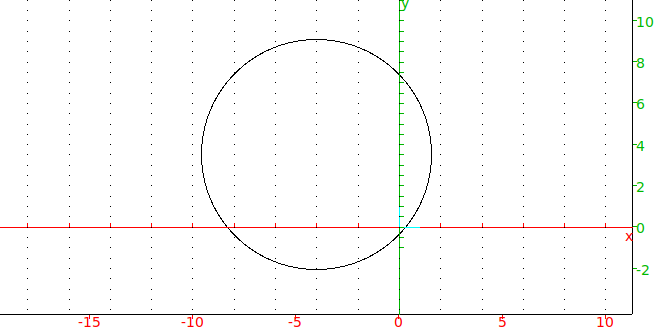
\includegraphics[width=0.75\textwidth]{xcas-osculatingcircle.png}
\end{center}
\item
\textit{Input:}
\begin{center}
  \texttt{equation(osculating\_circle(plot(x\^{}2),point(1,1)))}
\end{center}
\textit{Output:}
\[
\left(x+4\right)^{2}+\left(y-\frac{7}{2}\right)^{2}=\frac{125}{4}
\]
% \begin{center}
%   \tt
%  (x+4)\^{}2+(y-7/2)\^{}2=(125/4)
% \end{center}
\item
\textit{Input:}
\begin{center}
  \texttt{equation(osculating\_circle([t\^{}2,t\^{}3],t,1))}
\end{center}
\textit{Output:}
\[
\left(x+\frac{11}{2}\right)^{2}+\left(y-\frac{16}{3}\right)^{2}=\frac{2197}{36}
\]
% \begin{center}
%   \tt
%  (x+11/2)\^{}2+(y-16/3)\^{}2=(2197/36)
% \end{center}
\end{itemize}

\smallskip

The \texttt{evolute} command finds and draws the evolute of a curve.

To find the evolute from a parameterization:
\begin{itemize}
  \item \texttt{evolute} takes two arguments:
  \begin{itemize}
    \item $C$, a curve.
    \item $t$, the parameter of the curve.
  \end{itemize}
  \item \texttt{evolute($C,t$)} draws and returns the
  evolute of the curve.
\end{itemize}

\smallskip

To find the evolute from a curve object:
\begin{itemize}
  \item \texttt{evolute} takes one argument:\\
  $C$, a curve.
  \item \texttt{evolute($C$)} draws and returns the
  evolute of $C$.
\end{itemize}


\smallskip

\noindent
\textbf{Examples.}
\begin{itemize}
\item 
\textit{Input:}
\begin{center}
  \texttt{evolute(plot(x\^{}2))}
\end{center}
\textit{Output:}
\begin{center}
  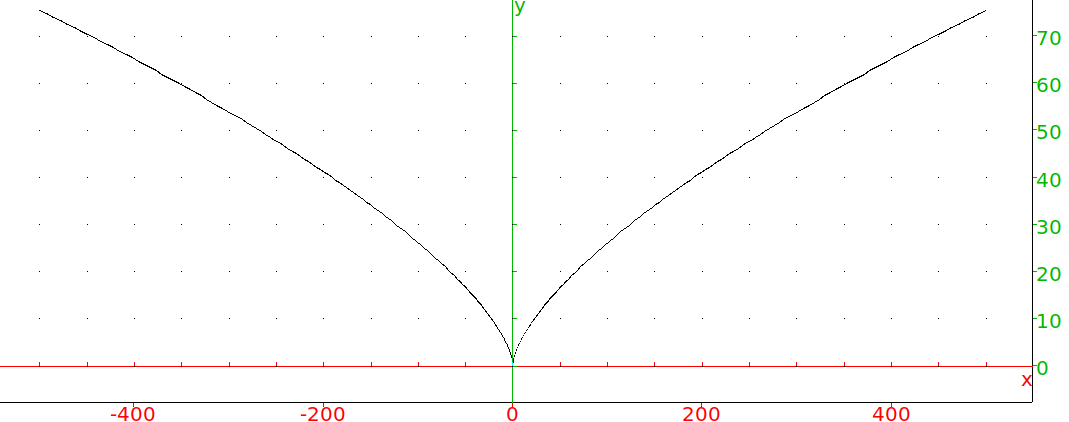
\includegraphics[width=0.75\textwidth]{xcas-evolute.png}
\end{center}
\item
\textit{Input:}
\begin{center}
  \texttt{equation(evolute(plot(x\^{}2)))}
\end{center}
\textit{Output:}
\[
27 x^{2}-16 y^{3}+24 y^{2}-12 y+2=0
\]
% \begin{center}
%   \tt
%  27*x\^{}2-16*y\^{}3+24*y\^{}2-12*y+2=0
% \end{center}
\item
\textit{Input:}
\begin{center}
  \texttt{equation(evolute([t\^{}2,t],t))}
\end{center}
\textit{Output:}
\[
16 x^{3}-24 x^{2}+12 x-27 y^{2}-2=0
\]
% \begin{center}
%   \tt
%  16*x\^{}3-24*x\^{}2+12*x-27*y\^{}2-2=0
% \end{center}
\end{itemize}

\chapter{Graphs\label{chap:plot}}

\section{Generalities}

Most graph instructions take expressions as arguments. A few
exceptions (mostly Maple-compatibility instructions) also accept
functions.  Some optional arguments, like \texttt{color, thickness},
can be used as optional attributes in all graphic instructions. They
are described below.

If a graph depends on a user-defined function, you may want to define
the function when the parameter is a formal variable.  For this, it
can be useful to test the type of the parameter while the function is
being defined.  (See Chapter \secref{chap:programming} for information
about programming in \texttt{Xcas}.)

For example, suppose \texttt{f} and \texttt{g} are defined by:\\
\begin{center}
\begin{tabular}{l}
\verb|f(x):= {|\\
\verb|  if (type(x)!=DOM_FLOAT) return 'f'(x);|\\
\verb|  while(x>0){ x--;}|\\
\verb|  return x;|\\
\verb|}|
\end{tabular}
\end{center}
and
\begin{center}
\begin{tabular}{l}
\verb|g(x):= {|\\
\verb|  while(x>0){ x--;}|\\
\verb|  return x;|\\
\verb|}:;|
\end{tabular}
\end{center}
Graphing these (see \secref{ssec:plotfunc}):\\
\textit{Input:}
\begin{center}
\begin{tabular}{l}
  \texttt{F:= plotfunc(f(x))}\\
  \texttt{G:= plotfunc(g(x))}
\end{tabular}
\end{center}
they will both produce the same graph.  However, the graphic
\texttt{G} won't be reusable.  Entering:\\
\textit{Input:}
\begin{center}
  \texttt{F}
\end{center}
reproduces the graph, but entering:\\
\textit{Input:}
\begin{center}
  \texttt{G}
\end{center}
produces the error:\\
\textit{Output:}
\begin{center}
\begin{tabular}{l}
  \texttt{"Unable to eval test in loop: x>0.0}\\
  \texttt{Error: Bad Argument Value Error:}\\
  \texttt{Bad Argument Value"}
\end{tabular}
\end{center}
Internally, \texttt{F} and \texttt{G} contain the formal expressions
\texttt{f(x)} and \texttt{g(x)}, respectively.  When \texttt{Xcas}
tries to evaluate \texttt{F} and \texttt{G},  \texttt{x} has no value
and so the test \texttt{x > 0} produces an error in \texttt{g(x)}, but
the line \verb|if (type(x)!=DOM_FLOAT) return 'f'(x);| avoids this
problem in \texttt{f(x)}.

\section{The graphic screen
\label{sec:graphscreen}}

A graphic screen, either two- or three-dimensional as appropriate,
automatically opens in response to a graphic command.  Alternatively,
you can open a graphic screen with its own command line with keystrokes;
\texttt{Alt-g} for a two-dimensional screen and \texttt{Alt-h} for a
three-dimensional screen. The graphic screen will have an array of
buttons at the top right.
\begin{itemize}
  \item There will be red arrows for moving the image in the $x$ direction.
  \item There will be green arrows for moving the image in the $y$
  direction.
  \item There will be blue arrows for zooming in and out in a
  two-dimensional screen, and moving the image in the $z$ direction in
  a three-dimensional screen.
  \item There will be \texttt{in} and \texttt{out} buttons for zooming
  in and out.
  \item There will be a \texttt{\_|\_} button to orthonormalize the
  graphic.
  \item There will be a \texttt{$\blacktriangleright$|} button to
  start and stop animations.
  \item There will be an \texttt{auto} button to do automatic scaling.
  \item There will be a \texttt{cfg} button which will bring up a
  configuration screen (see \secref{ssec:confcomp}).
  \item There will be an \texttt{M} button which brings up a menu.
  The menu has submenus:
  \begin{itemize}
    \item \texttt{View} which has entries which do the same as the
    buttons.
    \item \texttt{Trace} for working with traces.
    \item \texttt{Animation} for working with animations.
    \item \texttt{3-d} for working with three-dimensional graphics.
    \item \texttt{Export/Print} to export and print the graphic.
  \end{itemize}
\end{itemize}

The image can also be moved in the screen by clicking and dragging
with the mouse.  Scrolling with the mouse will also zoom the images.

\section{Graph and geometric objects attributes}

There are two kinds of attributes for graphs and geometric objects:
global attributes of a graphic scene and individual attributes.

\subsection{Individual attributes
\label{ssec:indattr}
\index{color@\textit{color}|textbf}
\index{display@\textit{display}|textbf}
\index{black@\texttt{black}}
\index{white@\texttt{white}}
\index{red@\texttt{red}}
\index{blue@\texttt{blue}}
\index{green@\texttt{green}}
\index{magenta@\texttt{magenta}}
\index{cyan@\texttt{cyan}}
\index{yellow@\texttt{yellow}}
\index{rhombus\_point@\texttt{rhombus\_point}}
\index{plus\_point@\texttt{plus\_point}}
\index{square\_point@\texttt{square\_point}}
\index{cross\_point@\texttt{cross\_point}}
\index{triangle\_point@\texttt{triangle\_point}}
\index{star\_point@\texttt{star\_point}}
\index{point\_point@\texttt{point\_point}}
\index{invisible\_point@\texttt{invisible\_point}}
\index{point\_width\_1@\texttt{point\_width\_1}}
\index{point\_width\_2@\texttt{point\_width\_2}}
\index{point\_width\_3@\texttt{point\_width\_3}}
\index{point\_width\_4@\texttt{point\_width\_4}}
\index{point\_width\_5@\texttt{point\_width\_5}}
\index{point\_width\_6@\texttt{point\_width\_6}}
\index{point\_width\_7@\texttt{point\_width\_7}}
\index{line\_width\_1@\texttt{line\_width\_1}}
\index{line\_width\_2@\texttt{line\_width\_2}}
\index{line\_width\_3@\texttt{line\_width\_3}}
\index{line\_width\_4@\texttt{line\_width\_4}}
\index{line\_width\_5@\texttt{line\_width\_5}}
\index{line\_width\_6@\texttt{line\_width\_6}}
\index{line\_width\_7@\texttt{line\_width\_7}}
\index{dash\_line@\texttt{dash\_line}}
\index{solid\_line@\texttt{solid\_line}}
\index{dashdot\_line@\texttt{dashdot\_line}}
\index{dashdotdot\_line@\texttt{dashdotdot\_line}}
\index{cap\_flat\_line @\texttt{cap\_flat\_line}}
\index{cap\_square\_line@\texttt{cap\_square\_line}}
\index{cap\_round\_line@\texttt{cap\_round\_line}}
\index{quandrant1@\texttt{quandrant1}}
\index{quandrant2@\texttt{quandrant2}}
\index{quandrant3@\texttt{quandrant3}}
\index{quandrant4@\texttt{quandrant4}}
\index{hidden\_name@\texttt{hidden\_name}}
\index{filled@\texttt{filled}}
\index{gl\_texture@\texttt{gl\_texture}}
\index{gl\_material@\texttt{gl\_material}}}

Graphic attributes are optional arguments of the form
\texttt{display=}\textit{value}.  They must be given as the last
argument of a graphic instruction. Attributes are ordered in several
categories: color, point shape, point width, line style, line
thickness, legend value, position and presence.  In addition, surfaces
may be filled or not, 3-d surfaces may be filled with a texture, 3-d
objects may also have properties with respect to the light.
Attributes of different categories may be combined with \texttt{+}, e.g. \\
\texttt{plotfunc($x^2+y^2$,[x,y],display=red+line\_width\_3+filled)}

The graphic attributes are:
\begin{itemize}
\item Colors, set with \texttt{display=}\textit{value} or
\texttt{color=}\textit{value}.  The values can be:
\begin{itemize}
\item \texttt{black}, \texttt{white}, \texttt{red}, \texttt{blue}, \texttt{green},
\texttt{magenta}, \texttt{cyan}, \texttt{yellow},
\item a numeric value between 0 and 255,
\item a numeric value between 256 and 256+7*16+14 for a color of the
rainbow,
\item any other numeric value smaller than 65535, the rendering
is not guaranteed to be portable.
\end{itemize}
\item Point shapes, set with \texttt{display=}\textit{value}.  The
values can be:
\begin{itemize}
  \item \texttt{rhombus\_point plus\_point}
  \item \texttt{square\_point cross\_point}
  \item \texttt{triangle\_point}
  \item \texttt{star\_point}
  \item \texttt{point\_point}
  \item \texttt{invisible\_point}
\item Point width, set with \texttt{display=}\textit{value}.  The
  values can be:\\
  \texttt{point\_width\_$n$} where $n$ is an
  integer between 1 and 7.
  \item Line thickness, set with \texttt{thickness=$n$}
    or \texttt{display=line\_width\_$n$} where $n$ is an
  integer between 1 and 7.
  \item Line shape, set with \texttt{display=}\textit{value}.  The
  values can be:
  \begin{itemize}
    \item \texttt{dash\_line}
    \item \texttt{solid\_line}
    \item \texttt{dashdot\_line}
    \item \texttt{dashdotdot\_line}
    \item \texttt{cap\_flat\_line}
    \item \texttt{cap\_square\_line}
    \item \texttt{cap\_round\_line}
  \end{itemize}
  \item Legend, the text is set with
  \texttt{legend=}\textit{"legendname"}; 
    the position is set with \texttt{display=}\textit{value}, where
    the values can be:
    \begin{itemize}
      \item \texttt{quadrant1}
      \item \texttt{quadrant2}
      \item \texttt{quadrant3}
      \item \texttt{quadrant4}
    \end{itemize}
    and correspond to the position of the legend of the object
    (using the trigonometric plane conventions).
    The legend is not displayed if the attribute
    \texttt{display=hidden\_name} is added.
    \item \texttt{display=filled} specifies that surfaces will be filled,
    \item \texttt{gl\_texture=}\textit{"picture\_filename"} is used to
    fill a surface with a texture. Cf. the interface manual for a more
    complete description and for \texttt{gl\_material=} options.
 \end{itemize}

\smallskip

\noindent
\textbf{Examples.}\\
(See \secref{ssec:2dgenpolygon}, \secref{ssec:2dpoint},
\secref{sssec:display} and \secref{ssec:2dsegments} for information on
the commands used.)
\begin{itemize}
\item 
\textit{Input:}
\begin{center}
\texttt{polygon(-1,-i,1,2*i,legend="P")}
\end{center}
\textit{Output:}
\begin{center}
  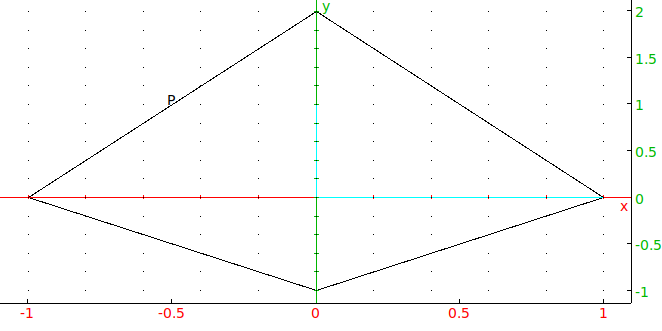
\includegraphics[width=0.75\textwidth]{xcas-attr01.png}
\end{center}
\item
\textit{Input:}
\begin{center}
\texttt{point(1+i,legend="hello")}
\end{center}
\textit{Output:}
\begin{center}
  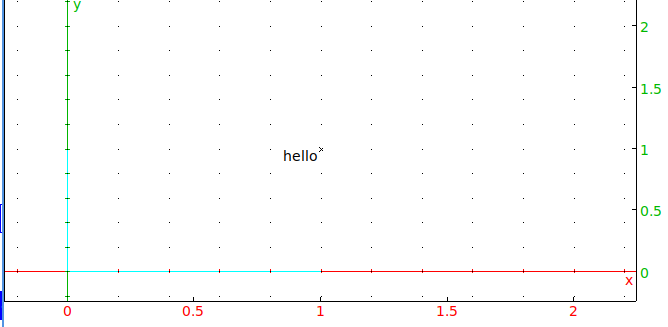
\includegraphics[width=0.75\textwidth]{xcas-attr02.png}
\end{center}
% \item
% \textit{Input:}
% \begin{center}
% \texttt{A:=point(1+i);B:=point(-1);display(D:=droite(A,B),hidden\_name)}
% A:=point(1+i);B:=point(-1);display(D:=droite(A,B),hidden_name)
% \end{center}
% \textit{Output:}
% \begin{center}
%   \includegraphics[width=0.75\textwidth]{xcas-attr03.png}
% \end{center}
\item
\textit{Input:}
\begin{center}
\texttt{color(segment(0,1+i),red)}
\end{center}
\textit{Output:}
\begin{center}
  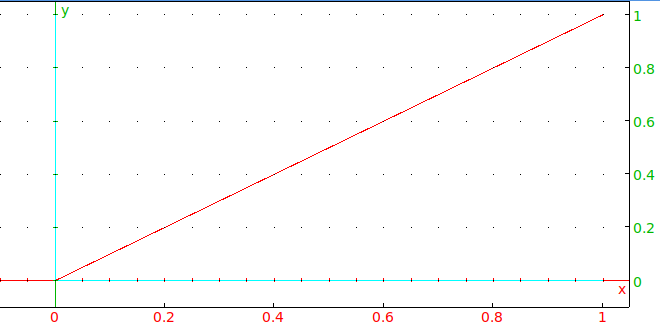
\includegraphics[width=0.75\textwidth]{xcas-attr04.png}
\end{center}
\item
\textit{Input:}
\begin{center}
\texttt{segment(0,1+i,color=red)}
\end{center}
\textit{Output:}
\begin{center}
  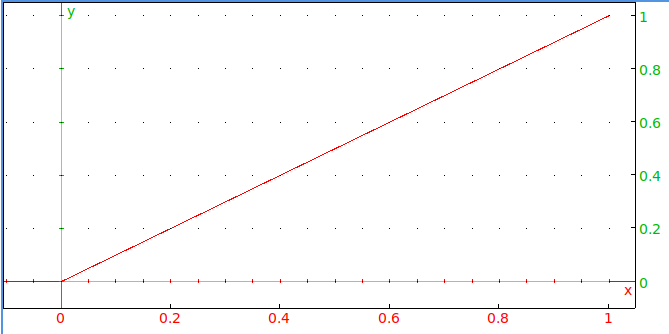
\includegraphics[width=0.75\textwidth]{xcas-attr05.png}
\end{center}
\end{itemize}

\subsection{Global attributes
\index{title@\textit{title}}
\index{labels@\textit{labels}}
\index{gl\_x\_axis\_name@\textit{gl\_x\_axis\_name}}
\index{gl\_y\_axis\_name@\textit{gl\_y\_axis\_name}}
\index{gl\_z\_axis\_name@\textit{gl\_z\_axis\_name}}
\index{gl\_x\_axis\_unit@\textit{gl\_x\_axis\_unit}}
\index{gl\_y\_axis\_unit@\textit{gl\_y\_axis\_unit}}
\index{gl\_z\_axis\_unit@\textit{gl\_z\_axis\_unit}}
\index{legend@\textit{legend}}
\index{axes@\textit{axes}}
\index{gl\_texture@\textit{gl\_texture}}
\index{gl\_x@\textit{gl\_x}}
\index{gl\_y@\textit{gl\_y}}
\index{gl\_z@\textit{gl\_z}}
\index{gl\_x\_tick@\textit{gl\_x\_tick}}
\index{gl\_y\_tick@\textit{gl\_y\_tick}}
\index{gl\_z\_tick@\textit{gl\_z\_tick}}
\index{gl\_shownames@\textit{gl\_shownames}}
\index{gl\_rotation@\textit{gl\_rotation}}
\index{gl\_quaternion@\textit{gl\_quaternion}}}

These attributes are shared by all objects of the same scene
\begin{itemize}
\item \texttt{title=}\textit{"titlename"} sets the title.
\item \texttt{labels=[}\textit{"xname","yname","zname"}\texttt{]} sets
names of the $x,y,z$ axes.
\item \texttt{gl\_x\_axis\_name=}\textit{"xname"},
\texttt{gl\_y\_axis\_name=}\textit{"yname"},
\texttt{gl\_z\_axis\_name=}\textit{"zname"} sets the names of the axes
individually.
\item \texttt{legend=[}\textit{"xunit","yunit","zunit"}\textit{]} sets
units for the axes.
\item \texttt{gl\_x\_axis\_unit=}\textit{"xunit"},
\texttt{gl\_y\_axis\_unit=}\textit{"yunit"},
\texttt{gl\_z\_axis\_unit=}\textit{"zunit"} sets units for the axes
individually.
\item \texttt{axes=true} or \texttt{axes=false} shows or hides the axis.
\item \texttt{gl\_texture=}\textit{"filename"} sets the background
image to \textit{"filename"}.
\item \texttt{gl\_x=}\textit{xmin..xmax}, \texttt{gl\_y=}\textit{ymin..ymax},
\texttt{gl\_z=}\textit{zmin..zmax} sets the graphic configuration
(do not use for interactive scenes)
\item \texttt{gl\_xtick=}\textit{xmark},
\texttt{gl\_ytick=}\textit{ymark}, \texttt{gl\_ztick=}\textit{zmark}
sets the tick marks for the axes.
\item \texttt{gl\_shownames=true} or \texttt{gl\_shownames=false}
shows or hides objects names
\item \texttt{gl\_rotation=[$x,y,z$]}: defines the rotation axis
for the animation rotation of 3-d scenes.
\item \texttt{gl\_quaternion=[$x,y,z,t$]}: defines the quaternion
for the visualization in 3-d scenes (do not use for interactive
scenes)
\item a few other OpenGL light configuration options are
available but not described here.
\end{itemize}

\smallskip

\noindent
\textbf{Examples.}
\begin{itemize}
% \item 
% \textit{Input:}
% \begin{center}
% \texttt{legend=["mn","kg"]}
% \end{center}
\item
\textit{Input:}
\begin{center}
\texttt{title="median\_line";triangle(-1-i,1,1+i);median\_line(-1-i,1,1+i);median\_line(1,-1-i,1+i);median\_line(1+i,1,-1-i)}
\end{center}
\textit{Output:}
\begin{center}
  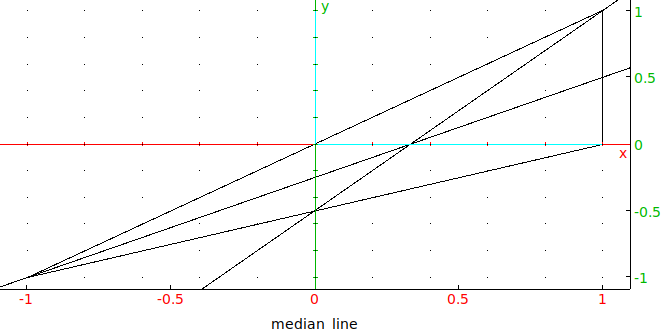
\includegraphics[width=0.75\textwidth]{xcas-gattr02.png}
\end{center}
\item
\textit{Input:}
\begin{center}
\texttt{labels=["u","v"];plotfunc(u+1,u)}
\end{center}
\textit{Output:}
\begin{center}
  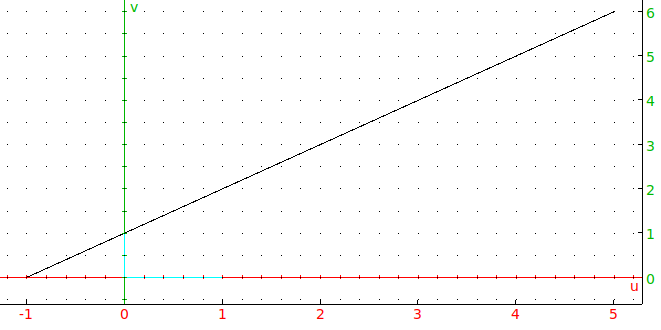
\includegraphics[width=0.75\textwidth]{xcas-gattr03.png}
\end{center}
\end{itemize}

\section{Graph of a function: \texttt{plotfunc} \texttt{funcplot}
\texttt{DrawFunc} \texttt{Graph} \index{plotfunc|textbf}
\index{funcplot|textbf} \index{DrawFunc|textbf} \index{Graph|textbf}
\index{xstep@{\sl xstep}} \index{ystep@{\sl ystep}} \index{zstep@{\sl
zstep}} \index{nstep@{\sl nstep}}
\label{sec:plotfunc}}

\subsection{2-d graph\label{ssec:plotfunc}}

The \texttt{plotfunc} command draws the graph of a function.\\
\texttt{funcplot} is a synonym for \texttt{plotfunc}.

\texttt{plotfunc} can draw the graph of a one-variable function or a
two-variable function; this section will discuss one-variable
functions and the next section will discuss two-variable functions.

\begin{itemize}
  \item \texttt{plotfunc} takes one mandatory argument and two
  optional arguments:
  \begin{itemize}
    \item \textit{expr}, an expression defining a function.
    \item Optionally, \textit{var}, the variable name (by default
    \texttt{x}) possibly with bounds.  If the variable is given as
    \textit{var=a..b}, the graph will be drawn from $a$ to $b$,
    otherwise it will be graphed over the default interval 
    (see \secref{ssec:confgraph}).
    \item Optionally, \textit{opt}, which can be
      \texttt{xstep=$n$} to specify the discretization
      step or \texttt{nstep=$n$} to specify the number of points used to
      graph.
  \end{itemize}
  \item
  \texttt{plotfunc(}\textit{expr,var}$\,\langle$\textit{opt}$\rangle$\texttt{)}
  draws the graph.
\end{itemize}

\smallskip

\noindent
\textbf{Examples.}
\begin{itemize}
\item 
\textit{Input:}
\begin{center}
\texttt{plotfunc(x\^{}2-2)}
\end{center}
\textit{Output:}
\begin{center}
  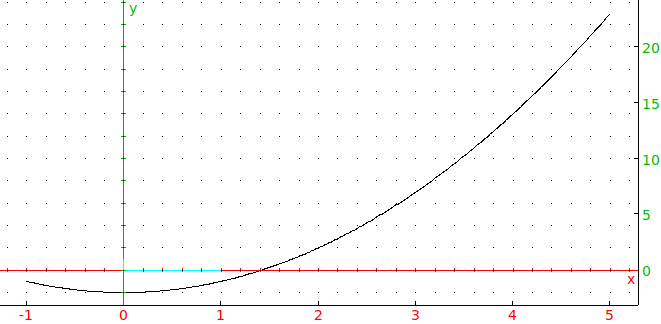
\includegraphics[width=0.75\textwidth]{xcas-plotf01.png}
\end{center}
\item
\textit{Input:}
\begin{center}
\texttt{plotfunc(a\^{}2-2,a=-1..2)}
\end{center}
\textit{Output:}
\begin{center}
  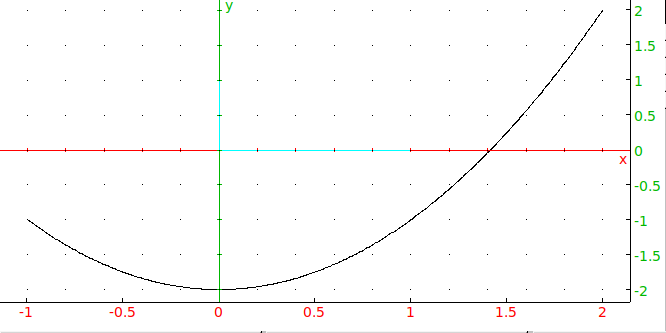
\includegraphics[width=0.75\textwidth]{xcas-plotf02.png}
\end{center}
% Output:
% \begin{center}\texttt{the graph of y=x\^{}2-2}\end{center}
\item
\textit{Input:}
\begin{center}
\texttt{plotfunc(x\^{}2-2,x,xstep=5)}
\end{center}
\textit{Output:}
\begin{center}
  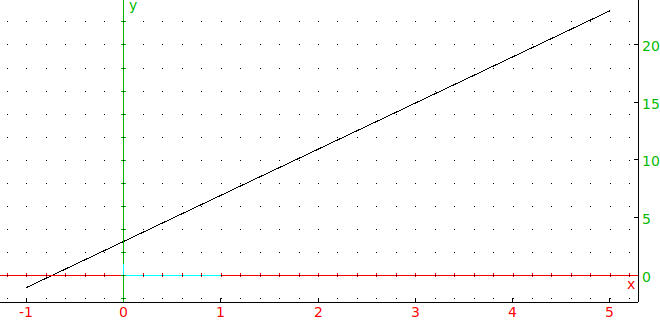
\includegraphics[width=0.75\textwidth]{xcas-plotf03.png}
\end{center}
% \begin{center}\texttt{a polygonal line which is a bad representation of y=x\^{}2-2}\end{center}
% It is also possible to specify the number of points used for the
% representation of the function with \verb|nstep=| instead of \verb|xstep=|.
% For example, input:
\item
\textit{Input:}
\begin{center}
\texttt{plotfunc(x\^{}2-2,x=-2..3,nstep=30)}
\end{center}
\textit{Output:}
\begin{center}
  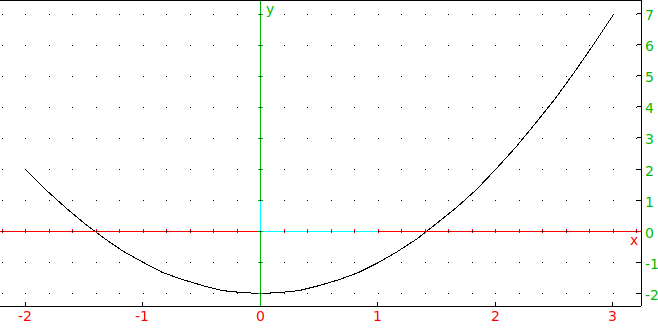
\includegraphics[width=0.75\textwidth]{xcas-plotf04.png}
\end{center}
\end{itemize}

\subsection{3-d graph\label{ssec:plotfunc3}}

\subsubsection{Two variable functions}

The \texttt{plotfunc} can draw the graphs of two-variable function.
\begin{itemize}
  \item \texttt{plotfunc} takes two mandatory argument and two
  optional arguments:
  \begin{itemize}
    \item \textit{expr}, an expression defining a function of two
    variables or a list of such expressions.
    \item \textit{vars}, a list of the variable names,
    possibly with bounds.  If the variable is given as
    \textit{var=a..b}, the graph will be drawn for that range of that
    variable, otherwise it will be graphed over the default interval 
    (see \secref{ssec:confgraph}).
    \item Optionally, \textit{xstep}, which can be
      \texttt{xstep=$n$} to specify the discretization
      step in the $x$ direction.
    \item Optionally, \textit{ystep}, which can be
      \texttt{ystep=$m$} to specify the discretization
      step in the $y$ direction.
    \item Instead of \textit{xstep} and \texttt{ystep}, you could use
      the option \texttt{nstep=$n$} to specify the number of points used to 
      graph.
  \end{itemize}
  \item
  \texttt{plotfunc(}\textit{expr,vars}$\,\langle$\textit{xstep,ystep}$\rangle$\texttt{)}
  draws the graph.
\end{itemize}

\smallskip

\noindent
\textbf{Examples.}
\begin{itemize}
\item 
\textit{Input:}
\begin{center}
\texttt{plotfunc(x\^{}2+y\^{}2,[x,y])}
\end{center}
\textit{Output:}
\begin{center}
  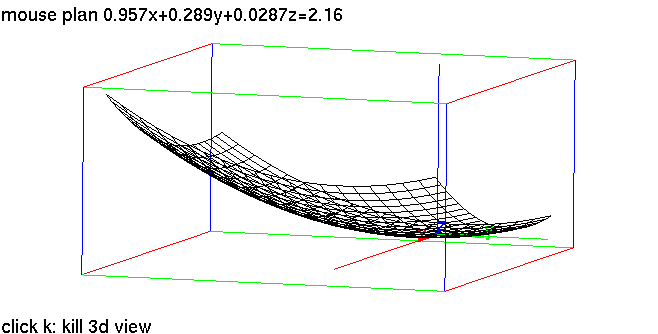
\includegraphics[width=0.75\textwidth]{xcas-3dplotf01.png}
\end{center}
\item
\textit{Input:}
\begin{center}
\texttt{plotfunc(x*y,[x,y])}
\end{center}
\textit{Output:}
\begin{center}
  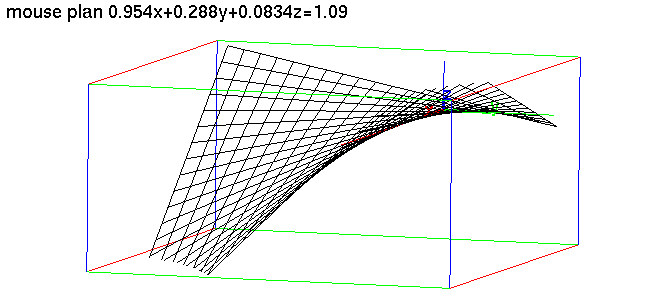
\includegraphics[width=0.75\textwidth]{xcas-3dplotf02.png}
\end{center}
\item
\textit{Input:}
\begin{center}
\texttt{plotfunc([x*y-10,x*y,x*y+10],[x,y])}
\end{center}
\textit{Output:}
\begin{center}
  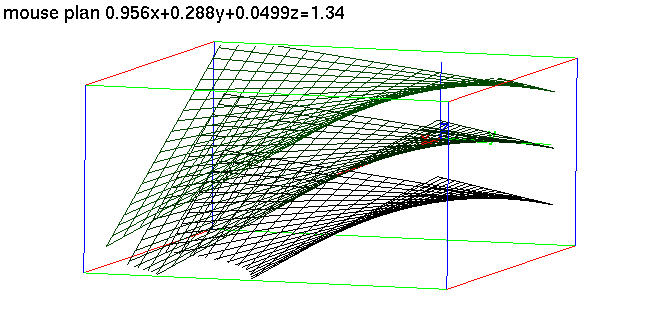
\includegraphics[width=0.75\textwidth]{xcas-3dplotf03.png}
\end{center}
\item
\textit{Input:}
\begin{center}
\texttt{plotfunc(x*sin(y),[x=0..2,y=-pi..pi])}
\end{center}
\textit{Output:}
\begin{center}
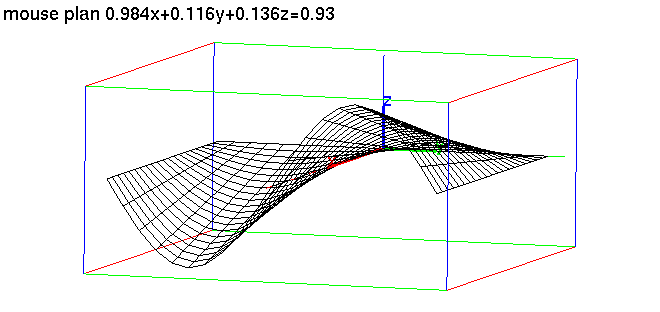
\includegraphics[width=0.75\textwidth]{xcas-3dplotf04.png}
\end{center}
\item
As an example where you specify the $x$ and $y$ discretization step
with \texttt{xstep} and \texttt{ystep}:\\
\textit{Input:}
\begin{center}
\texttt{plotfunc(x*sin(y),[x=0..2,y=-pi..pi],xstep=1,ystep=0.5)}
\end{center}
\textit{Output:}
\begin{center}
  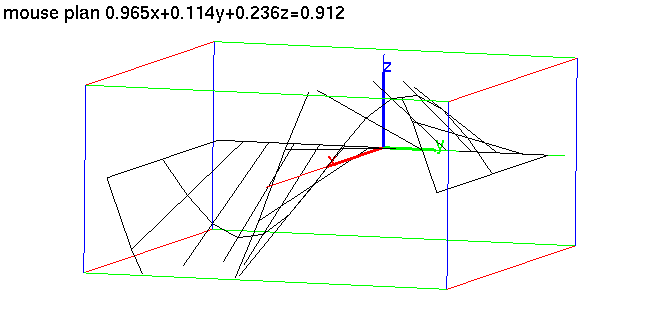
\includegraphics[width=0.75\textwidth]{xcas-3dplotf05.png}
\end{center}
\item
Alternatively you can specify
the number of points used for the representation of the
function with \texttt{nstep} instead of \texttt{xstep} and
\texttt{ystep}.\\
\textit{Input:}
\begin{center}
\texttt{plotfunc(x*sin(y),[x=0..2,y=-pi..pi],nstep=300)}
\end{center}
\textit{Output:}
\begin{center}
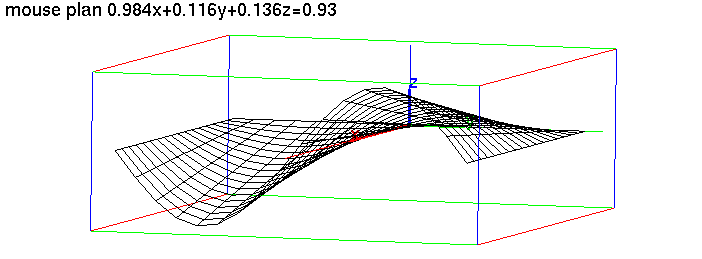
\includegraphics[width=0.75\textwidth]{xcas-3dplotf06.png}
\end{center}
\end{itemize}

\smallskip

\textbf{Remarks:}
\begin{itemize}
\item
Like any 3-d scene, the viewpoint may be modified by rotation
around the \texttt{x} axis, the \texttt{y} axis or the
\texttt{z} axis, either by dragging the mouse inside the graphic
window (push the mouse outside the parallelepiped used for
the representation), or with the shortcuts
\texttt{x}, \texttt{X}, \texttt{y}, \texttt{Y}, \texttt{z} and \texttt{Z}.
\item
If you want to print a graph or get a \LaTeX\ translation, use the graph
menu\\
\texttt{Menu$\blacktriangleright$print$\blacktriangleright$Print(with
  Latex)}
\end{itemize}

\subsubsection{3-d graph with rainbow colors\label{sssec:plotfunc3d}}

If the expression with two variables is purely
imaginary, \textit{$i$expr}, then \texttt{plotfunc} 
will still draw the graph, but the color will depend on the height
\textit{$z=$expr} resulting in a rainbow colored surface.   This
provides you with  an easy way to find points having the same third
coordinate.

\smallskip

\noindent
\textbf{Example.}\\
\textit{Input:}
\begin{center}
\texttt{plotfunc(i*x*sin(y),[x=0..2,y=-pi..pi])}
\end{center}
\textit{Output:}
\begin{center}
  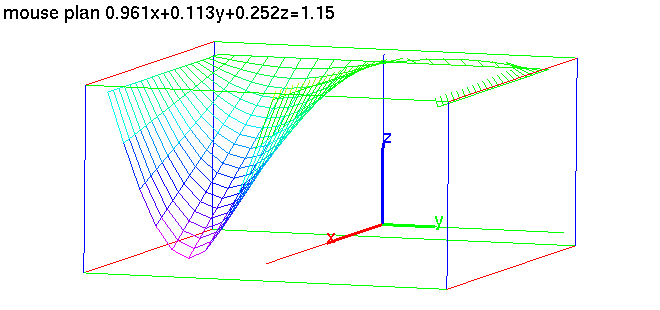
\includegraphics[width=0.75\textwidth]{xcas-3dplotf07.png}
\end{center}

\subsubsection{4-d graph\label{ssec:plotfunc4}}

If \textit{expr} is a complex valued expression whose real part is not
identically zero on the discretization mesh, then 
\texttt{plotfunc} will draw the surface
$z=$\texttt{abs(}\textit{expr}\texttt{)}, where
\texttt{arg(}\textit{expr}\texttt{)} determines the color from the
rainbow. This gives you an easy way to see the points 
having the same argument. Note that if the real part of \textit{expr}
is zero on the discretization mesh, then it will look purely imaginary
to \texttt{plotfunc} and will represented with rainbow colors, as in
\secref{sssec:plotfunc3d}.


\smallskip

\noindent
\textbf{Examples.}
\begin{itemize}
\item 
\textit{Input:}
\begin{center}
\texttt{plotfunc((x+i*y)\^{}2,[x,y])}
\end{center}
\textit{Output:}
\begin{center}
  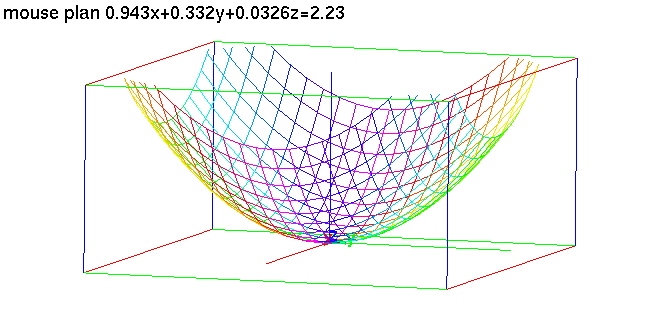
\includegraphics[width=0.75\textwidth]{xcas-3dplotf08.png}
\end{center}
\item
\textit{Input:}
\begin{center}
\texttt{plotfunc((x+i*y)\^{}2,[x,y], display=filled)}
\end{center}
\textit{Output:}
\begin{center}
  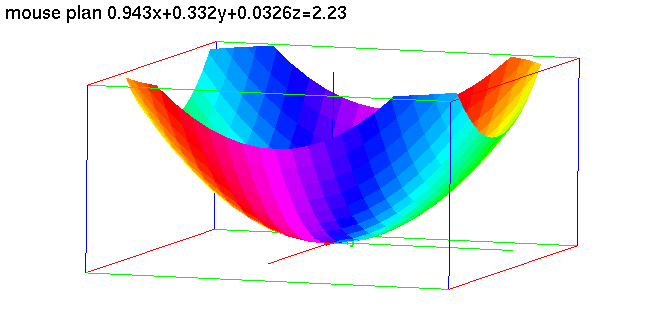
\includegraphics[width=0.75\textwidth]{xcas-3dplotf09.png}
\end{center}
\item
You can specify the range of variation of $x$ and $y$ and the number of
discretization points.\\
\textit{Input:}
\begin{center}
\texttt{plotfunc((x+i*y)\^{}2,[x=-1..1,y=-2..2], nstep=900,display=filled)}
\end{center}
\textit{Output:}
\begin{center}
  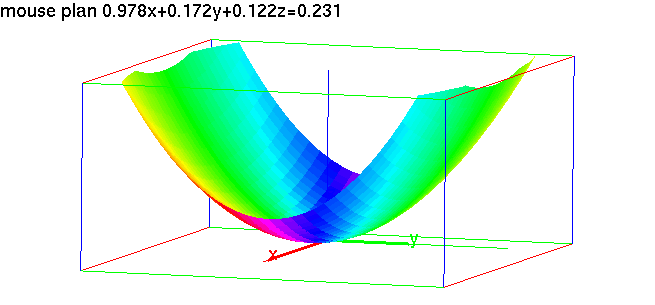
\includegraphics[width=0.75\textwidth]{xcas-3dplotf10.png}
\end{center}
\end{itemize}

\section{2d graph for Maple compatibility: \texttt{plot}
\label{sec:plot2d}
\index{plot}}

The \texttt{plot} command is a Maple-compatible way to draw the graph
of a one-variable function.
\begin{itemize}
  \item \texttt{plot} takes one mandatory argument and two optional
  arguments:
  \begin{itemize}
    \item \textit{func}, a function or an expression involving one
    variable. 
    \item Optionally, \textit{var} the name of the variable in the
    expression (if \textit{func} is an expression), which
    can also specify a range of values \textit{var=a..b} (by default
    it is \texttt{x}).  If \textit{func} is a function, the optional
    second argument can simply be a range \textit{a..b} for the
    variable.
    \item Optionally, \textit{opt}, which can be
    \texttt{xstep=$n$} to specify the discretization
    step or \texttt{nstep=$n$} to specify the number of points used to
    graph.
  \end{itemize}
  \item
  \texttt{plot(}\textit{expr$\,\langle ,$var, opt$\rangle$}\texttt{)}
  draws the graph.
\end{itemize}

\smallskip

\noindent
\textbf{Examples.}
\begin{itemize}
\item 
\textit{Input:}
\begin{center}
\texttt{plot(x\^{}2-2,x)}
\end{center}
\textit{Output:}
\begin{center}
  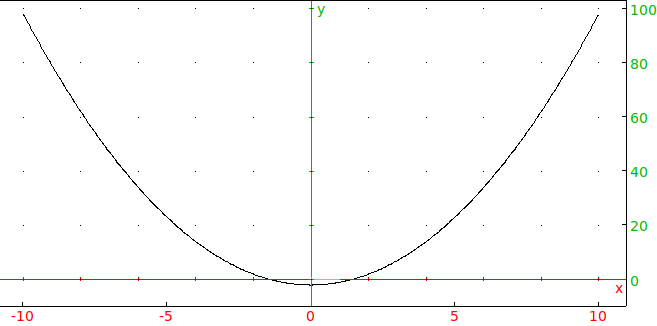
\includegraphics[width=0.75\textwidth]{xcas-mplot01.png}
\end{center}
%\begin{center}\texttt{the graph of y=x\^{}2-2}\end{center}
\item
\textit{Input:}
\begin{center}
\texttt{plot(x\^{}2-2,xstep=1)}
\end{center}
\textit{or:}
\begin{center}
\texttt{plot(x\^{}2-2,x,xstep=1)}
\end{center}
\textit{Output:}
\begin{center}
  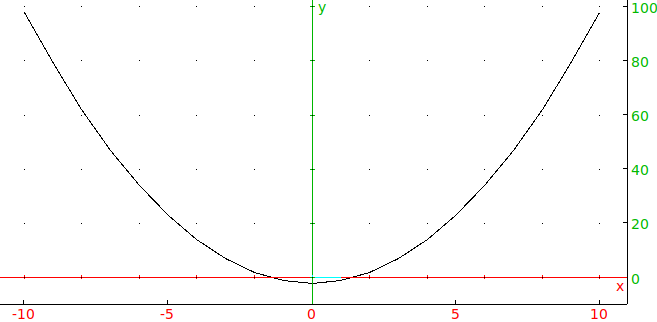
\includegraphics[width=0.75\textwidth]{xcas-mplot02.png}
\end{center}
%\begin{center}\texttt{a polygonal line which is a bad representation of
%    y=x\^{}2-2}\end{center}
\item
\textit{Input:}
\begin{center}
\texttt{plot(x\^{}2-2,x=-2..3,nstep=30)}
\end{center}
\textit{Output:}
\begin{center}
  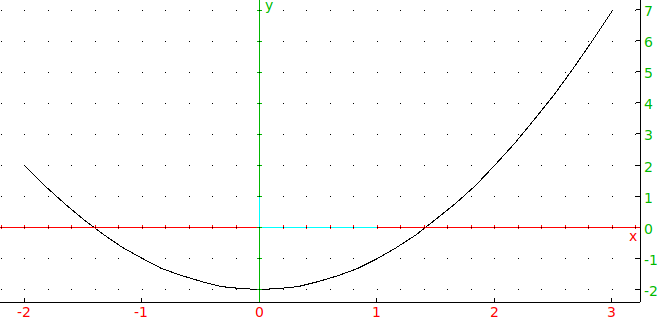
\includegraphics[width=0.75\textwidth]{xcas-mplot03.png}
\end{center}
\end{itemize}

\section{3d surfaces for Maple compatibility \texttt{plot3d}
\index{plot3d}
\label{sec:plot3d}}

The \texttt{plot3d} command is a Maple-compatible way to draw a surface.
It can plot the graph of a function of two variables or a surface
given by a parameterization.

To draw the graph of a function:
\begin{itemize}
  \item \texttt{plot3d} takes three arguments:
  \begin{itemize}
    \item \textit{func}, a function or an expression involving two
    variables. 
    \item $x$ and $y$, the names of the variable in the
    expression (if \textit{func} is an expression) which can also
    specify a range of values for each variable.
    
    If \textit{func} is a function, this argument is optional, and are
    the ranges \textit{a..b} for the variables.

    If the ranges are not given, the default values are taken from the
    graph configuration (see \secref{ssec:confgraph}).
  \end{itemize}
  \item
  \texttt{plot3d(}\textit{func$,x,y$}\texttt{)} draws the graph.
\end{itemize}


\smallskip

\noindent
\textbf{Example.}\\
\textit{Input:}
\begin{center}
\texttt{plot3d(x*y,x,y)}
\end{center}
\textit{Output:}
\begin{center}
  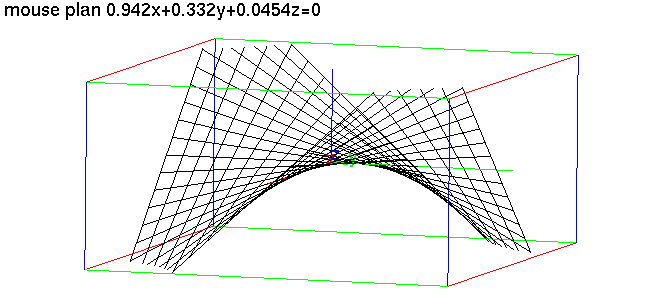
\includegraphics[width=0.75\textwidth]{xcas-3dmplot01.png}
\end{center}

\smallskip

To draw a parameterized surface:
\begin{itemize}
  \item \texttt{plot3d} takes one mandatory argument and two optional
  arguments:
  \begin{itemize}
    \item \textit{funcs}, a list of three functions or three
    expressions involving two variables. 
    \item $u$ and $v$, the names of the variable in the
    expression (if \textit{funcs} is a list of expressions),
    which can also specify a range of values for each variable.
    
    If \textit{funcs} is a list of functions, this argument is
    optional, and are the ranges \textit{a..b} for the variables.

    If the ranges are not given, the default values are taken from the
    graph configuration (see \secref{ssec:confgraph}).
  \end{itemize}
  \item
  \texttt{plot3d(}\textit{funcs$,u,v$}\texttt{)} draws the surface.
\end{itemize}

\smallskip

\noindent
\textbf{Examples.}
\begin{itemize}
\item 
\textit{Input:}
\begin{center}
\texttt{plot3d([v*cos(u),v*sin(u),v],u,v)}
\end{center}
\textit{Output:}
\begin{center}
  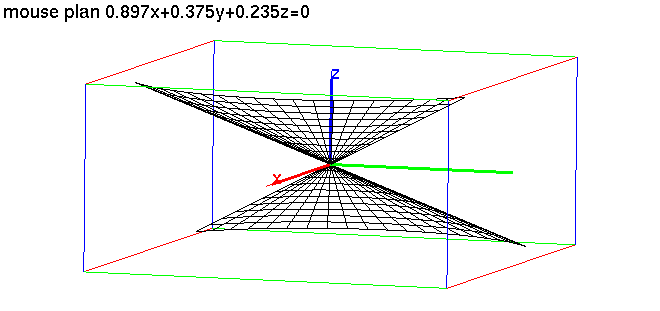
\includegraphics[width=0.75\textwidth]{xcas-3dmplot02.png}
\end{center}
% \textit{Output:}
% \begin{center}
% \texttt{The cone $x=v*\cos(u),y=v*\sin(u),z=v$}
% \end{center}
\item
\textit{Input:}
\begin{center}
\texttt{plot3d([v*cos(u),v*sin(u),v],u=0..pi,v=0..3)}
\end{center}
\textit{Output:}
\begin{center}
  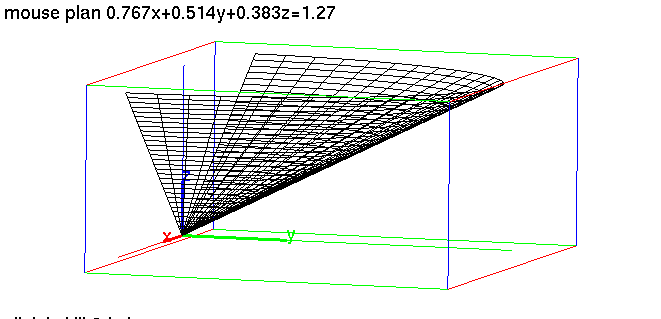
\includegraphics[width=0.75\textwidth]{xcas-3dmplot03.png}
\end{center}
% Output:
% \begin{center}\texttt{A portion of the cone $x=v*\cos(u),y=v*\sin(u),z=v$}\end{center}
\end{itemize}
\section{Graph of a line and tangent to a graph}

\subsection{Drawing a line: \texttt{line}\label{ssec:doite}
\index{line}}

%\textbf{See also:} \ref{sec:droite2} and \ref{sec:droite3} for line usage in
%geometry and see \ref{sec:axe2} and \ref{sec:axe3} for axis.\\

The \texttt{line} command draws and finds lines in $\mathbb{R}^{2}$
and $\mathbb{R}^{3}$.

For a line in $\mathbb{R}^{2}$:
\begin{itemize}
  \item \texttt{line} takes one argument:\\
  \textit{eqn}, a linear equation in the variables \texttt{x} and
  \texttt{y}.
  \item \texttt{line(}\textit{eqn}\texttt{)} draws and returns the
  line given by the equation.
\end{itemize}

\smallskip

\noindent
\textbf{Examples.}
\begin{itemize}
\item 
\textit{Input:}
\begin{center}
\texttt{line(2*y+x-1=0)}
\end{center}
\textit{Output:}
\begin{center}
  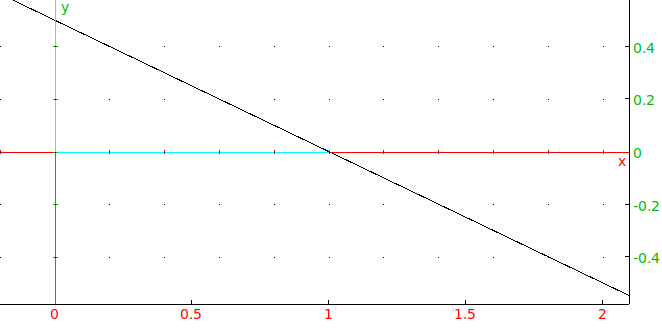
\includegraphics[width=0.75\textwidth]{xcas-line01.png}
\end{center}
%\begin{center}\texttt{the line 2*y+x-1=0}\end{center}
\item
\textit{Input:}
\begin{center}
\texttt{line(y=1)}
\end{center}
\textit{Output:}
\begin{center}
  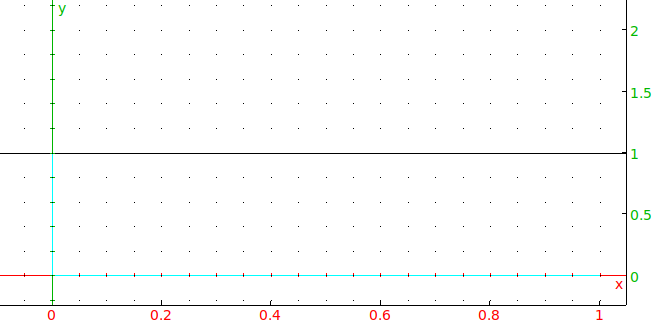
\includegraphics[width=0.75\textwidth]{xcas-line02.png}
\end{center}
%\begin{center}\texttt{the horizontal line y=1}\end{center}
\item
\textit{Input:}
\begin{center}
\texttt{line(x=1)}
\end{center}
\textit{Output:}
\begin{center}
  \includegraphics[width=0.75\textwidth]{xcas-line03.png}
\end{center}
%\begin{center}\texttt{the vertical line x=1}\end{center}
\end{itemize}

\smallskip

For a line in $\mathbb{R}^{3}$:
\begin{itemize}
  \item \texttt{line} takes two arguments:\\
  \textit{eqn1} and \texttt{eqn2}, two linear equations in the
  variables \texttt{x}, \texttt{y} and \texttt{z}.
  \item \texttt{line(}\textit{eqn1,eqn2}\texttt{)} draws and returns
  the line which is the intersection of the planes given by the
  equations.
\end{itemize}

\smallskip

\noindent
\textbf{Examples.}
\begin{itemize}
\item 
\textit{Input:}
\begin{center}
\texttt{line(x+2*y+z-1=0,z=2)}
\end{center}
\textit{Output:}
\begin{center}
  \includegraphics[width=0.75\textwidth]{xcas-line04.png}
\end{center}
%\begin{center}\texttt{the line x+2*y+1=0 in the plane z=2}\end{center}
\item
\textit{Input:}
\begin{center}
\texttt{line(y=1,x=1)}
\end{center}
\textit{Output:}
\begin{center}
\includegraphics[width=0.75\textwidth]{xcas-line05.png}
\end{center}
%\begin{center}\texttt{the vertical line crossing through (1,1,0)}\end{center}
\end{itemize}

\smallskip

\noindent
\textbf{Remark}\\
\texttt{line} defines an oriented line:
\begin{itemize}
\item When a 2D line is given by an equation, it is rewritten
as  \textit{lhs-rhs}$=ax+by+c=0$, this determines
its normal vector $[a,b]$ and the orientation is given by the vector
$[b,-a]$.
% (equivalently, its orientation is defined by the 3D cross
% product of its normal vectors (with third coordinate 0) and the vector [0,0,1]).\\
% For example \texttt{line(y=2*x)} defines the line \texttt{-2x+y=0} with as direction
% the vector \texttt{[1,2]} (or \texttt{cross([-2,1,0],[0,0,1])}=\texttt{[1,2,0]}).
\item When a 3D line is given by two plane equations, its
direction is defined by the cross product of the normals to the planes.

When the plane equation is rewritten as
\textit{lhs-rhs}$=ax+by+cz+d=0$
the normal is $[a,b,c]$.
For example, \texttt{line(x=y,y=z)} draws the line $x-y=0,y-z=0$ and its
direction is:
\[ 
[1,-1,0]\times [0,1,-1]=[1,1,1]
\]
\end{itemize}

\subsection{Drawing a 2D horizontal line: \texttt{LineHorz}
\index{LineHorz}}

The \texttt{LineHorz} command draws a horizontal line in $\mathbb{R}^{2}$.
\begin{itemize}
  \item \texttt{LineHorz} takes one argument:\\
  $a$, a number.
  \item \texttt{LineHorz($a$)} draws the horizontal line $y=a$.
\end{itemize}

\smallskip

\noindent
\textbf{Example.}\\
\textit{Input:}
\begin{center}
\texttt{LineHorz(1)}
\end{center}
\textit{Output:}
\begin{center}
  \includegraphics[width=0.75\textwidth]{xcas-hline01.png}
\end{center}
%\begin{center}\texttt{the line y=1}\end{center}

\subsection{Drawing a 2D vertical line: \texttt{LineVert}
\index{LineVert}}


The \texttt{LineVert} command draws a vertical line in $\mathbb{R}^{2}$.
\begin{itemize}
  \item \texttt{LineVert} takes one argument:\\
  $a$, a number.
  \item \texttt{LineVert($a$)} draws the vertical line $x=a$.
\end{itemize}

\smallskip

\noindent
\textbf{Example.}\\
\textit{Input:}
\begin{center}
\texttt{LineVert(1)}
\end{center}
\textit{Output:}
\begin{center}
  \includegraphics[width=0.75\textwidth]{xcas-vline01.png}
\end{center}
%\begin{center}\texttt{the line x=1}\end{center}

\subsection{Tangent to a 2D graph: \texttt{LineTan}
\index{LineTan}}

The \texttt{LineTan} command draws tangent lines to graphs.
\begin{itemize}
  \item \texttt{LineTan} takes two arguments:
  \begin{itemize}
    \item \textit{expr}, in the variable \texttt{x}.
    \item $x_{0}$, a value of \texttt{x}.
  \end{itemize}
  \item \texttt{LineTan(}\textit{expr}$,x_{0}$\texttt{)} draws the
  tangent at \texttt{x}$=x0$ to the graph of \textit{expr}.
\end{itemize}

\smallskip

\noindent
\textbf{Example.}\\
\textit{Input:}
\begin{center}
\texttt{LineTan(ln(x),1)}
\end{center}
\textit{Output:}
\begin{center}
  \includegraphics[width=0.75\textwidth]{xcas-tline01.png}
\end{center}
%\begin{center}\texttt{the line y=x-1}\end{center}
\textit{Input:}
\begin{center}
\texttt{equation(LineTan(ln(x),1))}
\end{center}
\textit{Output:}
\[
y=(x-1)
\]

\subsection{Tangent to a 2D graph: \texttt{tangent}\label{ssec:tangente}
\index{tangent|textbf}}

The \texttt{tangent} command draws tangents to surfaces.
%\textbf{See also:} \ref{sec:tangent} for plane geometry and
%\ref{sec:tangent3} for 3D geometry.\\
\begin{itemize}
  \item \texttt{tangent} takes two arguments:
  \begin{itemize}
    \item $S$, the graph of a two-variable function or a geometric
    object (see chapter \ref{chap:3dgraphics}).
    \item $A$, a point on $S$ or a number (if $S$ is a graph).
  \end{itemize}
  \item \texttt{tangent($S,A$)} draws tangent(s) to $S$ passing through
  $A$.
\end{itemize}

\smallskip

\noindent
\textbf{Example.}\\
Define the function \texttt{g}:\\
\textit{Input:}
\begin{center}
\texttt{g(x):=x\^{}2}
\end{center}
then the graph \texttt{G} of \texttt{g}  and a point $A$ on the graph:\\
\textit{Input:}
\begin{center}
\begin{tabular}{l}
\texttt{G:=plotfunc(g(x),x):;}\\
\texttt{A:=point(1.2,g(1.2)):;}
\end{tabular}
\end{center}
If you want to draw the tangent at the point \texttt{A} to the graph
\texttt{G}, you can enter:\\
\textit{Input:}
\begin{center}
\texttt{T:=tangent(G, A)}
\end{center}
\textit{or:}
\begin{center}
\texttt{T:=tangent(G, 1.2)}
\end{center}
\textit{Output:}
\begin{center}
  \includegraphics[width=0.75\textwidth]{xcas-2dtangent01.png}
\end{center}
For the equation of the tangent line, you can enter:\\
\textit{Input:}
\begin{center}
\texttt{equation(T)}
\end{center}
\textit{Output:}
\[
y=2.4 x-1.44
\]

\subsection{Plotting a line with a point and the slope: \texttt{DrawSlp}}
\index{DrawSlp}

The \texttt{DrawSlp} command can draw a line given a point and a slope.
\begin{itemize}
  \item \texttt{DrawSlp} takes three arguments:\\
  $a$, $b$ and $m$, real numbers.
  \item \texttt{DrawSlp($a,b,m$)} returns and draws the line through the
  point $(a,b)$ with slope $m$.
\end{itemize}

\smallskip

\noindent
\textbf{Example.}\\
\textit{Input:}
\begin{center}
  \texttt{DrawSlp(2,1,-1)}
\end{center}
\textit{Output:}
\begin{center}
  \includegraphics[width=0.75\textwidth]{xcas-DrawSlp.png}
\end{center}

\subsection{Intersection of a 2D graph with the axis
\index{solve}\index{resoudre}}

You can find the intersection of the graph $y=f(x)$ of a function with
the axes using the commands covered so far.
\begin{itemize}
\item Finding the intersection of the graph with the
$y$-axis is simply evaluating
\[
f(0),
\]
indeed the point with coordinates $(0,f(0))$ is the intersection point
of the graph of $f$ with the $y$-axis.
\item Finding the intersection of the graph of $f$ with the $x$-axis
requires solving the equation $f(x)=0$.
\begin{itemize}
  \item If $f(x)$ is polynomial-like, then you can find the 
  the exact values of the abscissa of these points with 
  \texttt{solve} (see \secref{ssec:solve}).\\
  \textit{Input:}
  \begin{center}
  \texttt{solve($f(x),x$)}
  \end{center}
  returns the solution.
  \item Otherwise, you can find numeric approximations of these
  abscissa. First, look at the graph for an initial guess $x_{0}$ or a 
  range with an intersection and then refine it with
  \texttt{fsolve} (see \secref{sec:fsolve}).\\
  \textit{Input:}
  \begin{center}
  \texttt{fsolve($f(x),x,x_{0},$}\textit{method}\texttt{)}
  \end{center}
  returns a numeric approximation of a solution.
\end{itemize}
\end{itemize}

\section{Graphing inequalities with two variables:
\texttt{plotinequation} \texttt{inequationplot}}
\index{plotinequation|textbf} \index{inequationplot|textbf}

The \texttt{plotinequation} command plots the region of the plane
where given inequalities hold.
\begin{itemize}
  \item \texttt{plotinequation} takes two arguments:
  \begin{itemize}
    \item \textit{ineqs}, a list of inequalities in two variables.
    \item \textit{vars}, a list of variables \textit{var} or variables 
    \textit{var=a..b}  with their ranges of values.
    Note that if the ranges are not specified,
  \texttt{Xcas} takes the default values of
  \texttt{X-,X+,Y-,Y+} defined in the general graphic configuration
  (\texttt{Cfg$\blacktriangleright$Graphic configuration}, see
  \secref{ssec:confgraph}).
  \end{itemize}
  \item \textit{plotinequation(}\textit{ineqs,vars}\texttt{)}
  draws the points of the plane whose coordinates satisfy the
  inequalities \textit{ineqs}.
\end{itemize}

\smallskip

\noindent
\textbf{Examples.}
\begin{itemize}
\item 
\textit{Input:}
\begin{center}
\texttt{plotinequation(x\^{}2-y\^{}2<3, [x=-2..2,y=-2..2],xstep=0.1,ystep=0.1)}
\end{center}
\textit{Output:}
\begin{center}
  \includegraphics[width=0.75\textwidth]{xcas-plotinequation01.png}
\end{center}
%\begin{center}\texttt{the filled portion enclosing the origin and limited by the hyperbola x\^{}2-y\^{}2=3}\end{center}
\item
\textit{Input:}
\begin{center}
\texttt{plotinequation([x+y>3,x\^{}2<y], [x-2..2,y=-1..10],xstep=0.2,ystep=0.2)}
\end{center}
\textit{Output:}
\begin{center}
  \includegraphics[width=0.75\textwidth]{xcas-plotinequation02.png}
\end{center}
%\begin{center}\texttt{the filled portion of the plane defined by -2<x<2,y<10,x+y>3,y>x\^{}2}\end{center}
\end{itemize}

\section{The area under a curve: \texttt{area}
\index{area}}

The \texttt{area} command approximates the area under a graph.
\begin{itemize}
  \item \texttt{area} takes four arguments:
  \begin{itemize}
    \item \textit{expr}, an expression $f(x)$.
    \item \textit{var=a..b}, the variable with a range.
    \item $n$, a positive integer.
    \item \textit{method}, the approximation method to use, which can
    be one of:
    \begin{itemize}
      \item \texttt{trapezoid}
      \item \texttt{left\_rectangle}
      \item \texttt{right\_rectangle}
      \item \texttt{middle\_point}
      \item \texttt{simpson}
      \item \texttt{rombergt} (Romberg with the trapezoid method)
      \item \texttt{rombergm} (Romberg with the midpoint method)
      \item \texttt{gauss15} (The 15 point Gaussian quadrature)
    \end{itemize}
  \end{itemize}
  \item \texttt{area(}\textit{expr,var=a..b,$n$,method}\texttt{)}
  returns an approximation to the area under the graph over the given
  interval, using the specified method with $n$ subdivisions (or $2^n$
  subdivisions for \texttt{rombert}, \texttt{rombergm} and
  \texttt{gauss15}).
\end{itemize}

\smallskip

\noindent
\textbf{Examples.}
\begin{itemize}
\item 
\textit{Input:}
\begin{center}
  \texttt{area(x\^{}2,x=0..1,8,trapezoid)}
\end{center}
\textit{Output:}
\[
0.3359375
\]
% \begin{center}
%   \tt
%  0.3359375
% \end{center}
\item
\textit{Input:}
\begin{center}
  \texttt{area(x\^{}2,x=0..1,8,rombergm)}
\end{center}
\textit{Output:}
\[
0.333333333333
\]
% \begin{center}
%   \tt
%   0.333333333333
% \end{center}
\item
\textit{Input:}
\begin{center}
  \texttt{area(x\^{}2,x=0..1,3,gauss15)}
\end{center}
\textit{Output:}
\[
0.333333333333
\]
% \begin{center}
%   \tt
% 0.333333333333
% \end{center}
\item
\textit{Input:}
\begin{center}
  \texttt{area(x\^{}2,x=0..1)}
\end{center}
\textit{Output:}
\[
\frac{1}{3}
\]
% \begin{center}
%   \tt
%  1/3
% \end{center}
\end{itemize}

\section{Graphing the area below a curve: \texttt{plotarea}
\texttt{areaplot}} \index{plotarea|textbf} \index{areaplot|textbf}
\index{rectangle\_droit@{\sl rectangle\_droit}|textbf}
\index{rectangle\_gauche@{\sl rectangle\_gauche}|textbf}
\index{trapeze@{\sl trapeze}|textbf} \index{point\_milieu@{\sl
point\_milieu}|textbf}

The \texttt{plotarea} command draws the area below a graph.\\
\texttt{areaplot} is a synonym for \texttt{plotarea}.
\begin{itemize}
  \item \texttt{plotarea} takes two mandatory arguments and two
  optional arguments:
  \begin{itemize}
    \item \textit{expr}, an expression representing the function to
    graph.
    \item \textit{var=a..b}, the variable and the range of values.
    \item Optionally, $n$.
    \item Optionally, \texttt{method}, a method to approximate the
    region under the graph, which can be one of:
    \begin{itemize}
      \item \texttt{trapezoid}
      \item \texttt{rectangle\_left}
      \item \texttt{rectangle\_right}
      \item \texttt{middle\_point}
    \end{itemize}
  \end{itemize}
  \item \texttt{plotarea(}\textit{expr,var=a..b}\texttt{)}
  draws and shades the area between the graph of \textit{expr} and the 
  $y$-axis for \textit{a < var < b}.
  \item \texttt{plotarea(}\textit{expr,var=a..b$\,\langle, n$,
  method$\rangle$}\texttt{)}
  draws and shades the region used by the numeric approximation method
  \textit{method} for area between the graph of \textit{expr} and the 
  $y$-axis for \textit{a < var < b}, when $[a,b]$ is cut into $n$
  equal parts, along with the graph in red.
\end{itemize}

\smallskip

\noindent
\textbf{Examples.}
\begin{itemize}
\item 
\textit{Input:}
\begin{center}
\texttt{plotarea(sin(x),x=0..2*pi)}
\end{center}
\textit{Output:}
\begin{center}
  \includegraphics[width=0.75\textwidth]{xcas-plotarea01.png}
\end{center}
%\begin{center}\texttt{the portion of plane locates in the two arches of sin(x)}\end{center}
\item
\textit{Input:}
\begin{center}
\texttt{plotarea(x\^{}2,x=0..1,5,trapezoid)}
\end{center}
% If you want to display the graph of the curve in contrast
% (e.g. in bold red), input:
% \begin{center}
% \texttt{plotarea(x\^{}2,x=0..1,5,trapezoid);plot(x\^{}2,x=0..1,display=red+line\_width\_3)}
% \end{center}
\textit{Output:}
\begin{center}
  \includegraphics[width=0.75\textwidth]{xcas-plotarea02.png}
\end{center}
%\begin{center}\texttt{the 5 trapezoids used in the trapezoid method to approach the integral}\end{center}
\textit{Input:}
\begin{center}
\texttt{plotarea((x\^{}2,x=0..1,5,middle\_point)}
\end{center}
% Or with the graph of the curve in bold red, input:
% \begin{center}
% \texttt{plotarea(x\^{}2,x=0..1,5,middle\_point); plot(x\^{}2,x=0..1,display=red+line\_width\_3)}
% \end{center}
\textit{Output:}
\begin{center}
  \includegraphics[width=0.75\textwidth]{xcas-plotarea03.png}
\end{center}
%\begin{center}\texttt{the 5 rectangles used in the middle\_point method
%    to approach the integral}\end{center}
\end{itemize}

\section{Contour lines: \texttt{plotcontour} \texttt{contourplot}
\texttt{DrwCtour}\label{sec:plotcontour} \index{plotcontour|textbf}
\index{contourplot|textbf} \index{DrwCtour|textbf}}

The \texttt{plotcontour} command draws contour lines for functions of
two variables.\\
\texttt{DrwCtour} and \texttt{contourplot} are synonyms for
\texttt{plotcontour}.
\begin{itemize}
  \item \texttt{plotcontour} takes two mandatory arguments and one
  optional argument:
  \begin{itemize}
    \item \textit{expr}, an expression involving two variables.
    \item \textit{vars}, a list of the two variables.
    \item Optionally, \textit{values}, a list of values of the contour
    lines to draw; \textit{expr=value}, for \textit{value} in
    \textit{values}  (by default, $[-10,-8,\dots,8,10]$).
  \end{itemize}
  \item \texttt{plotcontour(}\textit{expr,vars$\,\langle$,
  values$\rangle$}\texttt{)} draws the contour lines 
  \textit{expr=value} for \textit{value} in \textit{values}.
  \end{itemize}

\smallskip

\noindent
\textbf{Examples.}
\begin{itemize}
\item 
\textit{Input:}
\begin{center}
\texttt{plotcontour(x\^{}2+y\^{}2,[x=-3..3,y=-3..3],[1,2,3], display=[green,red,black]+[filled\$3])}
\end{center}
\textit{Output:}
\begin{center}
  \includegraphics[width=0.75\textwidth]{xcas-plotcontour01.png}
\end{center}
%\begin{center}\texttt{the graph of the three ellipses x\^{}2-y\^{}2=n for n=1,2,3; the zones between these ellipses are filled with the color green,red or black}\end{center}
\item
\textit{Input:}
\begin{center}
\texttt{plotcontour(x\^{}2-y\^{}2,[x,y])}
\end{center}
\textit{Output:}
\begin{center}
  \includegraphics[width=0.75\textwidth]{xcas-plotcontour02.png}
\end{center}
%\begin{center}\texttt{the graph of 11 hyperbolas x\^{}2-y\^{}2=n for n=-10,-8,..10}\end{center}
\end{itemize}

\smallskip

If you want to draw the surface in 3-d representation, you can use
\texttt{plotfunc} (see \secref{ssec:plotfunc3}).\\
\textit{Input:}
\begin{center}
\texttt{plotfunc(x\^{}2-y\^{}2,[x,y])}
\end{center}
\textit{Output:}
\begin{center}
  \includegraphics[width=0.75\textwidth]{xcas-plotcontour03.png}
\end{center}
%\begin{center}\texttt{A 3D representation of z=x\^{}2+y\^{}2}\end{center}

\section{2-d graph of a 2-d function with colors: \texttt{plotdensity}
\texttt{densityplot} \index{plotdensity|textbf}
\index{densityplot|textbf}}

The \texttt{plotdensity} command draws the graph of a function of two
variables in the plane where the values of $z$ are represented by the
rainbow colors.\\
\texttt{densityplot} is a synonym for \texttt{plotdensity}.
\begin{itemize}
  \item \texttt{plotdensity} takes two mandatory arguments and three
  optional arguments:
  \begin{itemize}
    \item \textit{expr}, an expression of two variables.
    \item \textit{vars}, a list of the variables and their ranges.
    \item Optionally, \texttt{z=}$a..b$, the range of $z$ to
    correspond to the full rainbow (by default, it is deduced from the
    minimum and maximum value of \textit{expr} on the discretization.
    \item Optionally, \textit{xstep}, which can be
      \texttt{xstep=$n$} to specify the discretization
      step in the $x$ direction.
    \item Optionally, \textit{ystep}, which can be
      \texttt{ystep=$m$} to specify the discretization
      step in the $y$ direction.
    \item Instead of \textit{xstep} and \texttt{ystep}, you could use
      the option \texttt{nstep=$n$} to specify the number of points used to 
      graph.
  \end{itemize}
  \item
  \texttt{plotdensity(}\textit{expr,vars$\,\langle$}\texttt{z=}\textit{$a..b$,xstep,ystep}\texttt{$\rangle$)}
  draws the graph of \textit{expr} in the plane where the values of
  $z$ are represented by the rainbow colors.
\end{itemize}
\textbf{Remark}: A rectangle representing the scale of colors will be
displayed below the graph.

\smallskip

\noindent
\textbf{Example.}\\
\textit{Input:}
\begin{center}
\texttt{plotdensity(x\^{}2-y\^{}2,[x=-2..2,y=-2..2], xstep=0.1,ystep=0.1)}
\end{center}
\textit{Output:}
\begin{center}
  \includegraphics[width=0.75\textwidth]{xcas-plotdensity01.png}
\end{center}
% \begin{center}\texttt{A 2D graph where each hyperbola defined by
%     x\^{}2-y\^{}2=z has a color from the rainbow}\end{center}

\section{Implicit graph: \texttt{plotimplicit} \texttt{implicitplot}}
\index{plotimplicit} \index{implicitplot} \index{unfactored}

The \texttt{plotimplicit} command draws curves
or surfaces defined by an implicit expression or equation.  If the
option \texttt{unfactored} is given as the last argument, the original
expression is taken unmodified. Otherwise, the expression is
normalized, then replaced by the factorization of the numerator of its
normalization.

Each factor of the expression corresponds to a component of the
implicit curve or surface. For each factor, \texttt{Xcas} tests if it
is of total degree less or equal to 2, in which case \texttt{conic} or
\texttt{quadric} is called. Otherwise the numeric implicit solver is
called.

Optional step and ranges arguments may be passed to the numeric
implicit solver, note that they are dismissed for each component that
is a conic or a quadric.

\texttt{implicitplot} is a synonym for \texttt{plotimplicit}.

\subsection{2D implicit curve\label{ssec:implicitplot}}

For an implicit plot in $\mathbb{R}^{2}$:
\begin{itemize}
  \item \texttt{plotimplicit} takes three mandatory arguments and
  three optional arguments:
  \begin{itemize}
    \item \textit{expr}, an expression of two variables implicitly
    defining a curve by \textit{expr=0}.
    \item \textit{vars}, a list of the two variables, optionally with
    their ranges \textit{var=a..b}.  If a range is not given, the
    ranges are determined by \texttt{WX-, WX+} and \texttt{WY-, WY+}
    in the graphical configuration (see \secref{ssec:confgraph}).
    \item Optionally, \textit{xstep}, which can be
      \texttt{xstep=$n$} to specify the discretization
      step in the $x$ direction.
    \item Optionally, \textit{ystep}, which can be
      \texttt{ystep=$m$} to specify the discretization
      step in the $y$ direction.
    \item Optionally, \texttt{unfactored}.
  \end{itemize}
  \item
  \texttt{plotimplicity(}\textit{expr,vars}$\,\langle$\textit{xstep,ystep,}\texttt{unfactored$\rangle$)}
  draws the graphic representation of the curve defined by the implicit equation 
  \textit{expr=0} over the given ranges of the variables.
\end{itemize}

\smallskip

\noindent
\textbf{Examples.}
\begin{itemize}
\item 
\textit{Input:}
\begin{center}
\texttt{plotimplicit(x\^{}2+y\^{}2-1,x,y)}
\end{center}
\textit{or:}
\begin{center}
\texttt{plotimplicit(x\^{}2+y\^{}2-1,x,y,unfactored)}
\end{center}
\textit{Output:}
\begin{center}
  \includegraphics[width=0.75\textwidth]{xcas-plotimplicit01.png}
\end{center}
%\begin{center}\texttt{The unit circle}\end{center}
\item
\textit{Input:}
\begin{center}
\texttt{plotimplicit(x\^{}2+y\^{}2-1,x,y,xstep=0.2,ystep=0.3)}
\end{center}
\textit{or:}
\begin{center}
\texttt{plotimplicit(x\^{}2+y\^{}2-1,[x,y],xstep=0.2,ystep=0.3)}
\end{center}
\textit{or:}
\begin{center}
\texttt{plotimplicit(x\^{}2+y\^{}2-1,[x,y], xstep=0.2,ystep=0.3,unfactored)}
\end{center}
\textit{Output:}
\begin{center}
  \includegraphics[width=0.75\textwidth]{xcas-plotimplicit02.png}
\end{center}
%\begin{center}\texttt{The unit circle}\end{center}
\item
\textit{Input:}
\begin{center}
\texttt{plotimplicit(x\^{}2+y\^{}2-1,x=-2..2,y=-2..2, xstep=0.2,ystep=0.3)}
\end{center}
\textit{Output:}
\begin{center}
  \includegraphics[width=0.75\textwidth]{xcas-plotimplicit03.png}
\end{center}
%\begin{center}\texttt{The unit circle}\end{center}
\end{itemize}

\subsection{3D implicit surface\label{ssec:implicitplot3}}

For an implicit plot in $\mathbb{R}^{2}$:
\begin{itemize}
  \item \texttt{plotimplicit} takes four mandatory arguments and
  three optional arguments:
  \begin{itemize}
    \item \textit{expr}, an expression of three variables implicitly
    defining a curve by \textit{expr=0}.
    \item \textit{xvar}, \textit{yvar} and \textit{zvar}, the first,
    second and third variables,optionally with
    their ranges \textit{var=a..b}.
    % If a range is not given, the
    % ranges are determined by \texttt{WX-, WX+} and \texttt{WY-, WY+}
    % in the graphical configuration (see \secref{ssec:confgraph}).
    \item Optionally, \textit{xstep}, which can be
      \texttt{xstep=$n$} to specify the discretization
      step in the $x$ direction.
    \item Optionally, \textit{ystep}, which can be
      \texttt{ystep=$m$} to specify the discretization
      step in the $y$ direction.
    \item Optionally, \textit{zstep}, which can be
      \texttt{zstep=$p$} to specify the discretization
      step in the $y$ direction.
    \item Optionally, \texttt{unfactored}.
  \end{itemize}
  \item
  \texttt{plotimplicity(}\textit{expr,xvar,yvar,zvar}$\,\langle$\textit{xstep,ystep,zstep}\texttt{unfactored$\rangle$)}
  draws the graphic representation of the surface defined by the implicit equation 
  \textit{expr=0} over the given ranges of the variables.
\end{itemize}

\smallskip

\noindent
\textbf{Examples.}
\begin{itemize}
\item 
\textit{Input:}
\begin{center}
\texttt{plotimplicit(x\^{}2+y\^{}2+z\^{}2-1,x,y,z, xstep=0.2,ystep=0.1,zstep=0.3)}
\end{center}
\textit{or:}
\begin{center}
\texttt{plotimplicit(x\^{}2+y\^{}2+z\^{}2-1,x,y,z, xstep=0.2,ystep=0.1,zstep=0.3,unfactored)}
\end{center}
\textit{Output:}
\begin{center}
\includegraphics[width=0.5\textwidth]{xcas-plotimplicitsphere.png}
\end{center}
%\begin{center}\texttt{The unit sphere}\end{center}
\item
\textit{Input:}
\begin{center}
\texttt{plotimplicit(x\^{}2+y\^{}2+z\^{}2-1,x=-1..1,y=-1..1,z=-1..1)}
\end{center}
\textit{Output:}
\begin{center}
\includegraphics[width=0.5\textwidth]{xcas-plotimplicitsphere2.png}
\end{center}
%\begin{center}\texttt{The unit sphere}\end{center}
\end{itemize}

\section{Parametric curves and surfaces: \texttt{plotparam}
\texttt{paramplot} \texttt{DrawParm} \index{plotparam|textbf}
\index{paramplot|textbf} \index{DrawParm|textbf}}

The \texttt{plotparam} command draws parametric curves and surfaces.\\
\texttt{paramplot} and \texttt{DrawParm} are synonyms for
\texttt{plotparam}.

\subsection{2D parametric curve}

To draw a parametric curve in $\mathbb{R}^{2}$:
\begin{itemize}
  \item \texttt{plotparam} takes two mandatory and one optional
  argument:
  \begin{itemize}
    \item \textit{exprs}, a list of two real expressions or one
    complex expression involving the parameter.
    \item \textit{var}, the parameter, optionally with a range
    \textit{var=a..b}.  If no range is given, the values of
    \texttt{t-} and \texttt{t+} from the graphics configuration will
    be used (see \secref{ssec:confgraph}).
    \item Optionally, \texttt{tstep=$n$}, to set the discretization
    step.
  \end{itemize}
  \item \texttt{plotparam(}\textit{exprs,var}\texttt{$\,\langle
  ,$tstep=$n\rangle$)} draws the parametric representation of the curve.
\end{itemize}

\smallskip

\noindent
\textbf{Examples.}
\begin{itemize}
\item 
\textit{Input:}
\begin{center}
\texttt{plotparam(cos(x)+i*sin(x),x)}
\end{center}
\textit{or:}
\begin{center}
\texttt{plotparam([cos(x),sin(x)],x)}
\end{center}
\textit{Output:}
\begin{center}
  \includegraphics[width=0.75\textwidth]{xcas-plotparam01.png}
\end{center}
%\begin{center}\texttt{The unit circle}\end{center}
\item
\textit{Input:}
\begin{center}
\texttt{plotparam(sin(t)+i*cos(t),t=-4..1)}
\end{center}
\textit{or:}
\begin{center}
\texttt{plotparam(sin(x)+i*cos(x),x=-4..1)}
\end{center}
\textit{or (with \texttt{t-=4,t+=1} in the graphic configuration):}
\begin{center}
\texttt{plotparam(sin(t)+i*cos(t))}
\end{center}
\textit{Output:}
\begin{center}
  \includegraphics[width=0.75\textwidth]{xcas-plotparam02.png}
\end{center}
%\begin{center}\texttt{the arc (sin(-4)+i*cos(-4),sin(1)+i*cos(1)) of the unit circle}\end{center}
\textit{Input:}
\begin{center}
\texttt{plotparam(sin(t)+i*cos(t),t=-4..1,tstep=0.5)}
\end{center}
\textit{or (with \texttt{t-=4,t+=1} in the graphic configuration):}
\begin{center}
\texttt{plotparam(sin(t)+i*cos(t),t,tstep=0.5)}
\end{center}
\textit{Output:}
\begin{center}
  \includegraphics[width=0.75\textwidth]{xcas-plotparam03.png}
\end{center}
%\begin{center}\texttt{A polygon approaching the arc (sin(-4)+i*cos(-4),sin(1)+i*cos(1)) of the unit circle}\end{center}
\end{itemize}

\subsection{3D parametric surface: \texttt{plotparam} \texttt{paramplot} \texttt{DrawParm}
\index{plotparam}
\index{paramplot}
\index{DrawParm}
\label{ssec:3dplotparam}}

To draw a parametric surface in $\mathbb{R}^{3}$:
\begin{itemize}
  \item \texttt{plotparam} takes two mandatory arguments and two optional
  arguments:
  \begin{itemize}
    \item \textit{exprs}, a list of three expressions involving two
    parameters.
    \item \textit{vars}, a list of the parameters, optionally with a range
    \textit{var=a..b}.
    \item Optionally, \texttt{ustep=$n$}, to set the discretization
    step of the first parameter.
    \item Optionally, \texttt{vstep=$m$}, to set the discretization
    step of the second parameter.
  \end{itemize}
  \item \texttt{plotparam(}\textit{exprs,vars}\texttt{$\,\langle
  ,$ustep=$n$,vstep=$m\rangle$)} draws the parametric representation
  of the surface.
\end{itemize}

\smallskip

\noindent
\textbf{Examples.}
\begin{itemize}
\item 
\textit{Input:}
\begin{center}
\texttt{plotparam([v*cos(u),v*sin(u),v],[u,v])}
\end{center}
\textit{Output:}
\begin{center}
  \includegraphics[width=0.75\textwidth]{xcas-plotparam04.png}
\end{center}
%\begin{center}\texttt{The cone $x=v*\cos(u),y=v*\sin(u),z=v$}\end{center}
\item
\textit{Input:}
\begin{center}
\texttt{plotparam([v*cos(u),v*sin(u),v],[u=0..pi,v=0..3])}
\end{center}
\textit{Output:}
\begin{center}
  \includegraphics[width=0.75\textwidth]{xcas-plotparam05.png}
\end{center}
%\begin{center}\texttt{A portion of the cone $x=v*\cos(u),y=v*\sin(u),z=v$}\end{center}
\item
\textit{Input:}
\begin{center}
\texttt{plotparam([v*cos(u),v*sin(u),v],[u=0..pi,v=0..3],ustep=0.5,vstep=0.5)}
\end{center}
\textit{Output:}
\begin{center}
  \includegraphics[width=0.75\textwidth]{xcas-plotparam06.png}
\end{center}
%\begin{center}\texttt{A portion of the cone $x=v*\cos(u),y=v*\sin(u),z=v$}\end{center}
\end{itemize}

\section{Bezier curves: \texttt{bezier} \index{bezier}}

The Bezier curve with the control points $P_0,P_1,\dots,P_n$ is the curve
parameterized by $\sum_{j=0}^{n} \binom{n,j} t^j (1-t)^{n-j} P_{j}$.
\texttt{bezier} plots Bezier curves.
\begin{itemize}
  \item \texttt{bezier} takes an unspecified number of arguments:
  \begin{itemize}
    \item \textit{controls}, a sequence of control points.
    \item \texttt{plot}, the symbol.
  \end{itemize}
  \item \texttt{bezier(}\textit{controls}\texttt{,plot)}
  plots the Bezier curve with the
  given control points.
\end{itemize}

\smallskip

\noindent
\textbf{Examples.}
\begin{itemize}
\item 
\textit{Input:}
\begin{center}
  \texttt{bezier(1,1+i,2+i,3-i,plot)}
\end{center}
\textit{Output:}
\begin{center}
   \includegraphics[width=0.75\textwidth]{xcas-bezier1.png}
\end{center}
\item
\textit{Input:}
\begin{center}
  \texttt{bezier(point(0,0,0),point(1,1,0),point(0,1,1),plot)}
\end{center}
\textit{Output:}
\begin{center}
   \includegraphics[width=0.75\textwidth]{xcas-bezier2.png}
\end{center}
\end{itemize}

\smallskip

To get the parameterization of the curve, you can use
the \texttt{parameq} command (see \secref{ssec:2dparam}).

\smallskip

\noindent
\textbf{Examples.}
\begin{itemize}
\item 
\textit{Input:}
\begin{center}
  \texttt{parameq(bezier(1,1+i,2+i,3-i))}
\end{center}
\textit{Output:}
\[
\left(1-t\right)^{3}+3 t \left(1-t\right)^{2} \left(1+\mathrm{i}\right)+3 t^{2} \left(1-t\right) \left(2+\mathrm{i}\right)+t^{3} \left(3-\mathrm{i}\right)
\]
% \begin{center}
%   \tt
%   (1-t)\^{}3+3*t*(1-t)\^{}2*(1+i)+3*t\^{}2*(1-t)*(2+i)+t\^{}3*(3-i)
% \end{center}
\item
\textit{Input:}
\begin{center}
  \texttt{parameq(bezier(point([0,0,0]),point([1,1,0]),point([0,1,1])))}
\end{center}
\textit{Output:}
\[
\left[2 t \left(1-t\right),2 t \left(1-t\right)+t^{2},t^{2}\right]
\]
% \begin{center}
%   \tt
%     point[2*t*(1-t),2*t*(1-t)+t\^{}2,t\^{}2]
% \end{center}
\end{itemize}

\section{Defining curves in polar coordinates: \texttt{plotpolar}
\texttt{polarplot} \texttt{DrawPol} \texttt{courbe\_polaire}
\index{plotpolar|textbf} \index{polarplot|textbf}
\index{DrawPol|textbf} \index{courbe\_polaire|textbf}}

The \texttt{plotpolar} command draws a curve given in polar
coordinates.\\
\texttt{polarplot}, \texttt{DrawPol} and \texttt{courbe\_polaire} are
synonyms for \texttt{plotpolar}.
\begin{itemize}
  \item \texttt{polarplot} takes two arguments:
  \begin{itemize}
    \item \textit{expr}, an expression involving a variable (which
    will represent the angle).
    \item \texttt{var}, the variable.  This can optionally include the
    range \textit{var=a..b}.
    \item Optionally, \texttt{tstep=$n$} to specify the discretization.
  \end{itemize}
  \texttt{polarplot(}\textit{expr,var}\texttt{$\,\langle$,tstep=$n\rangle$)}
  draws the 
  curve defined by $\rho=$\textit{expr} for $\theta=$\textit{var}; in
  Cartesian coordinates that is the curve 
  \textit{(expr $\cos$var),expr $\sin$(var))}.
\end{itemize}

\smallskip

\noindent
\textbf{Examples.}
\begin{itemize}
\item 
\textit{Input}
\begin{center}
\texttt{plotpolar(t,t)}
\end{center}
\textit{Output:}
\begin{center}
  \includegraphics[width=0.75\textwidth]{xcas-plotpolar01.png}
\end{center}
%\begin{center}\texttt{The spiral $\rho$=t is plotted}\end{center}
\item
\textit{Input:}
\begin{center}
\texttt{plotpolar(t,t,tstep=1)}
\end{center}
\textit{or:}
\begin{center}
\texttt{plotpolar(t,t=0..10,tstep=1)}
\end{center}
\textit{Output:}
\begin{center}
  \includegraphics[width=0.75\textwidth]{xcas-plotpolar02.png}
\end{center}
%\begin{center}\texttt{A polygon line approaching the spiral $\rho$=t is plotted}\end{center}
\end{itemize}

\section{Graphing recurrent sequences: \texttt{plotseq}
\texttt{seqplot} \texttt{graphe\_suite}\label{sec:plotseq}
\index{plotseq} \index{seqplot} \index{graphe\_suite}}

The \texttt{plotseq} command draws the process of finding the terms of
a recurrent sequence.\\ 
\texttt{seqplot} and \texttt{graphe\_suite} are synonyms for
\texttt{plotseq}.
\begin{itemize}
  \item \texttt{plotseq} takes :
  \begin{itemize}
    \item \textit{expr}, an expression depending on a variable.
    \item \textit{var=a}, the variable and a beginning value.  (If
    \textit{var=}\texttt{x}, then the variable name can be omitted.)
     The $a$ value can be replaced by a list of three elements, 
     $[a,x_-,x_+]$ where $x_-..x_+$ will be passed as the range of the
     variable for the graph computation.
    \item \textit{n}, the ending value of the variable.
  \end{itemize}
  \item \texttt{plotseq(}\textit{expr,var=a,n}\texttt{)}
  draws the line $y=x$, the graph of $y=$\textit{expr}, and the $n$
  first terms of the recurrent sequence defined by: $u_0=a$, 
  $u_n=f(u_{n-1})$ where $f$ is the function determined by \textit{expr}. 
\end{itemize}

\smallskip

\noindent
\textbf{Example.}\\
\textit{Input:}
\begin{center}
\texttt{plotseq(sqrt(1+x),x=[3,0,5],5)}
\end{center}
\textit{Output:}
\begin{center}
  \includegraphics[width=0.75\textwidth]{xcas-plotseq01.png}
\end{center}
%\begin{center}\texttt{the graph of y=sqrt(1+x), of y=x and of the 5 first terms of the sequence u\_0=3 and u\_n=sqrt(1+u\_(n-1))}\end{center}

\section{Tangent field: \texttt{plotfield} \texttt{fieldplot}
\index{plotfield} 
\index{fieldplot}
\label{sec:plotfield}}

The \texttt{plotfield} command draws the tangent field of a
differential equation or a vector field.\\
\texttt{fieldplot} is a synonym for \texttt{plotfield}.

To draw the tangent field of a differential equation:
\begin{itemize}
  \item \texttt{plotfield} takes two mandatory arguments and one
  optional argument:
  \begin{itemize}
    \item \textit{expr}, an expression depending on two variables, a
    time variable and a dependent variable.
    \item \textit{vars}, a list of the two variables $[t,y]$, where
    $t$ is the time variable and $y$ is the dependent variable.  The
    variables can optionally include their ranges; $[t=a..b,y=c..d]$.
    \item Optionally, \texttt{ystep=$n$} to specify the discretization.
  \end{itemize}
  \item
  \texttt{plotfield(}\textit{expr,vars$\,\langle$}\texttt{,ystep=$n\rangle$)}
    draws the tangent field of the differential equation $y'=f(t,y)$.
\end{itemize}

\smallskip

\noindent
\textbf{Example.}\\
\textit{Input:}
\begin{center}
\texttt{plotfield(4*sin(t*y),[t=0..2,y=-3..7])}
\end{center}
\textit{Output:}
\begin{center}
  \includegraphics[width=0.75\textwidth]{xcas-plotfield01.png}
\end{center}
%\begin{center}\texttt{Segments with slope 4*sin(t*y), representing tangents, are plotting in different points}\end{center}

\smallskip

To draw a vector field:
\begin{itemize}
  \item \texttt{plotfield} takes two mandatory arguments and two
  optional arguments:
  \begin{itemize}
    \item $V$, a list of two expressions involving two variables.
    \item \textit{vars}, a list of the two variables.  The
    variables can optionally include their ranges \textit{var=}$a..b$.
    \item Optionally, \texttt{xstep=$n$} to specify the discretization
    of the first variable.
    \item Optionally, \texttt{ystep=$m$} to specify the discretization
    of the second variable.
  \end{itemize}
  \item \texttt{plotfield($V$,}\textit{vars}\texttt{$\,\langle
  ,$xstep=$n,$ystep=$m\rangle$)} draws the vector field given by $V$.
\end{itemize}

\smallskip

\noindent
\textbf{Example.}\\
\textit{Input:}
\begin{center}
\texttt{plotfield(5*[-y,x],[x=-1..1,y=-1..1])}
\end{center}
\textit{Output:}
\begin{center}
  \includegraphics[width=0.75\textwidth]{xcas-plotfield02.png}
\end{center}

\section{Plotting a solution of a differential equation:
\texttt{plotode} \texttt{odeplot} \index{plotode} \index{odeplot}
\label{sec:plotode}}

The \texttt{plotode} command draws solutions of differential equations.
\begin{itemize}
  \item \texttt{plotode} takes three mandatory arguments and one
  optional argument:
  \begin{itemize}
    \item \textit{expr} an expression depending on two or three
    variables, a time variable and one or two dependent variables.
    \item \textit{vars}, a list of the time variable and the dependent
    variable.  The time variable can
    optionally have a range of values, such as $t=a..b$.  The
    dependent variable can also be a vector of size two.
    \item \textit{init}, the initial values of the variables.
    \item Optionally, for when there are two dependent variables,
    \texttt{plane}, the symbol, to draw the solution in the plane.
  \end{itemize}
  \item \texttt{plotode(}\textit{expr,vars,init}\texttt{)}
  draws the solution of the differential equation $y'=$\textit{expr}
  (where $y$ is the dependent variable) passing through the initial
  point \textit{init}.
\end{itemize}
To compute the values of the solutions, see
\secref{ssec:odesolve}.

\smallskip

\noindent
\textbf{Examples.}
\begin{itemize}
\item 
\textit{Input:}
\begin{center}
\texttt{plotode(sin(t*y),[t,y],[0,1])}
\end{center}
\textit{Output:}
\begin{center}
  \includegraphics[width=0.75\textwidth]{xcas-plotode01.png}
\end{center}
%\begin{center}{The graph of the solution of y'=sin(t,y) crossing through the point (0,1)}\end{center}
\item
\textit{Input:}
\begin{center}
\texttt{S:=plotode([h-0.3*h*p, 0.3*h*p-p], [t,h,p],[0,0.3,0.7])}
\end{center}
\textit{Output:}
\begin{center}
  \includegraphics[width=0.75\textwidth]{xcas-plotode03.png}
\end{center}
% Output, the graph in the space of the solution of:
% \[ [h,p]'=[h-0.3 h*p, 0.3 h*p-p] \quad [h,p](0)=[0.3,0.7] \]
\item
% To have a 2-d graph (in the plane), use the option
% \texttt{plane}
\textit{Input (for a 2-d graph in the plane):}
\begin{center}
\texttt{S:=odeplot([h-0.3*h*p, 0.3*h*p-p], [t,h,p],[0,0.3,0.7],plane)}
\end{center}
\textit{Output:}
\begin{center}
  \includegraphics[width=0.75\textwidth]{xcas-plotode04.png}
\end{center}
\end{itemize}

\section{Interactive plotting of solutions of a differential equation:
\texttt{interactive\_plotode} \texttt{interactive\_odeplot}
\index{interactive\_plotode} \index{interactive\_odeplot}
\label{sec:iplotode}}

The \texttt{interactive\_plotode} command draws interactive tangent
fields of differential equations.\\
\texttt{interactive\_odeplot} is a synonym for
\texttt{interactive\_plotode}.
\begin{itemize}
  \item \texttt{interactive\_plotode} takes two arguments:
  \begin{itemize}
    \item \textit{expr} an expression depending on two or three
    variables, a time variable and one or two dependent variables.
    \item \textit{vars}, a list of the time variable and the dependent
    variable.
  \end{itemize}
  \item \texttt{interactive\_plotode(}\textit{expr,vars}\texttt{)}
  draws the tangent field of the differential equation
  $y'=$\textit{expr} (where $y$ is the dependent variable) in a new
  window.  In this window, one can click on a point to get the plot of
  the solution of $y'=$\textit{expr} passing through this point.
  
  You can further click to display several solutions. To stop, press
  the \texttt{Esc} key. 
\end{itemize}

\smallskip

\noindent
\textbf{Example.}\\
\textit{Input:}
\begin{center}
\texttt{interactive\_plotode(sin(t*y),[t,y])}
\end{center}
\textit{Output:}
\begin{center}
  \includegraphics[width=0.75\textwidth]{xcas-plotode02.png}
\end{center}
Solutions of the differential equation can be plotted by clicking on
an initial point.

\section{Animated graphs (2D, 3D or "4D")}

\texttt{Xcas} can display animated 2D, 3D or "4D" graphs.  This is
done first by computing a sequence of graphic objects, then after
completion, by displaying the sequence in a loop.
%\begin{itemize}
%\item 
To stop or start again the animation, click on the button
$\blacktriangleright \mid$ (to the left of \texttt{Menu}).
% \item
% The display time of each graphic object is specified in \texttt{animate} of the
% graph configuration (\texttt{cfg} button). Put a small time,
% to have a fast animation.
\item
% If \texttt{animate} is \texttt{0}, the animation is frozen,
% you can move in the sequence of objects one by one by clicking
% on the mouse in the graphic scene.
% \end{itemize}

\subsection{Animation of a 2D graph: \texttt{animate}
\index{animate}
\index{frames@{\sl frames}|textbf}}

The \texttt{animate} command creates two-dimensional animations
using graphs of functions depending on a parameter.  (See also
\secref{sec:plot2d}.)
\begin{itemize}
  \item \texttt{animate} takes three mandatory arguments and two optional
  arguments:
  \begin{itemize}
    \item \textit{expr}, an expression involving two
    variables, one of which will be regarded as the parameter.
    \item \textit{var} the name of the (non-parameter)
    variable in the expression, which can also specify a range of
    values \textit{var=a..b}.
    \item \textit{param} the name of the parameter, which can also
    specify a range of values.
    \item Optionally, \texttt{frames=$n$}, where $n$ is an integer specifying the
    number of frames.
    \item Optionally, \textit{opt}, which can be
    \texttt{xstep=$n$} to specify the discretization
    step or \texttt{nstep=$n$} to specify the number of points used to
    graph.
  \end{itemize}
  \item
  \texttt{animate(}\textit{expr,var,param,}\texttt{frames=$n\,\langle$}\textit{opt}\texttt{$\rangle$)}
  draws an animation consisting of graph of the function as the
  parameter varies.  
\end{itemize}

\smallskip

\noindent
\textbf{Examples.}
\begin{itemize}
\item 
\begin{center}
\texttt{animate(sin(a*x),x=-pi..pi,a=-2..2,frames=10,color=red)}
\end{center}
\textit{Output:}\\
The output is an animation beginning with:
\begin{center}
  \includegraphics[width=0.75\textwidth]{xcas-animate01.png}
\end{center}

\subsection{Animation of a 3D graph: \texttt{animate3d}
\index{animate3d}}

The \texttt{animate3d} command creates three-dimensional animations
using graphs of functions depending on a parameter.  (See also
\secref{ssec:plotfunc3}.)
\begin{itemize}
  \item \texttt{animate} takes three mandatory arguments and two optional
  arguments:
  \begin{itemize}
    \item \textit{expr}, an expression involving three
    variables, one of which will be regarded as the parameter.
    \item \textit{vars} a list of the the (non-parameter)
    variables in the expression, which can also specify ranges of
    values \textit{var=a..b}.
    \item \textit{param} the name of the parameter, which can also
    specify a range of values.
    \item Optionally, \texttt{frames=$n$}, where $n$ is an integer specifying the
    number of frames.
    \item Optionally, \textit{xstep}, which can be
      \texttt{xstep=$n$} to specify the discretization
      step in the $x$ direction.
    \item Optionally, \textit{ystep}, which can be
      \texttt{ystep=$m$} to specify the discretization
      step in the $y$ direction.
    \item Instead of \textit{xstep} and \texttt{ystep}, you could use
      the option \texttt{nstep=$n$} to specify the number of points used to 
      graph.
  \end{itemize}
  \item
  \texttt{animate3d(}\textit{expr,vars,param,}\texttt{frames=$n\,\langle$}\textit{opt}\texttt{,xstep=$n$, ystep=$m \rangle$)}
  draws an animation consisting of graph of the function as the
  parameter varies.  
\end{itemize}

\smallskip

\noindent
\textbf{Example.}\\
\textit{Input:}
\begin{center}
\texttt{animate3d(x\^{}2+a*y\^{}2,[x=-2..2,y=-2..2],a=-2..2, frames=10,display=red+filled)}
\end{center}
\textit{Output:}\\
The output is an animation beginning with:
\begin{center}
  \includegraphics[width=0.75\textwidth]{xcas-animate3d01.png}
\end{center}

\subsection{Animation of a sequence of graphic objects: \texttt{animation}
\index{animation}}

The \texttt{animation} command creates animations using sequences of
graphic objects, which can be graphs 
(see \secref{sec:plotfunc}) or not (see chapters \ref{chap:2dgraphics}
and \ref{chap:3dgraphics}).
The sequence of objects depends most of the time on a parameter and is
defined using the \texttt{seq} command but it is not mandatory. 
To define a sequence of graphic objects with \texttt{seq}, enter the definition
of the graphic object (depending on the parameter), the parameter
name, its minimum value, its maximum value maximum and optionally a
step value.
\begin{itemize}
  \item \texttt{animation} takes:
  \begin{itemize}
    \item \textit{objs}, a sequence of graphic objects.
  \end{itemize}
  \item \texttt{animation(}\textit{objs}\texttt{)} 
  draws an animation consisting of the sequence of objects.
\end{itemize}

\smallskip

\noindent
\textbf{Examples.}
\begin{itemize}
\item
\textit{Input:}
\begin{center}
\texttt{animation(seq(plotfunc(cos(a*x),x),a,0,10))}
\end{center}
\textit{Output:}\\
The output is an animation beginning with:
\begin{center}
  \includegraphics[width=0.75\textwidth]{xcas-animation01.png}
\end{center}
%\begin{center}\texttt{The sequence of the curves defined by $y=\cos(ax)$, for $a=0,1,2..10$}\end{center}
\item
\textit{Input:}
\begin{center}
\texttt{animation(seq(plotfunc(cos(a*x),x),a,0,10,0.5))}
\end{center}
\textit{or:}
\begin{center}
\texttt{animation(seq(plotfunc(cos(a*x),x),a=0..10,0.5))}
\end{center}
\textit{Output:}\\
The output is an animation beginning with:
\begin{center}
  \includegraphics[width=0.75\textwidth]{xcas-animation01.png}
\end{center}
%\begin{center}\texttt{The sequence of the curves defined by $y=\cos(ax)$, for $a=0,0.5,1,1.5..10$}\end{center}
\item
\textit{Input:}
\begin{center}
\texttt{animation(seq(plotfunc([cos(a*x),sin(a*x)],x=0..2*pi/a), a,1,10))}
\end{center}
\textit{Output:}\\
The output is an animation beginning with:
\begin{center}
  \includegraphics[width=0.75\textwidth]{xcas-animation03.png}
\end{center}
%\begin{center}\texttt{The sequence of two curves defined by $y=\cos(ax)$ and $y=\sin(ax)$, for $a=1..10$ and for $x=0..2\pi/a$}\end{center}
\item
\textit{Input:}
\begin{center}
\texttt{animation(seq(plotparam([cos(a*t),sin(a*t)], t=0..2*pi),a,1,10))}
\end{center}
\textit{Output:}\\
The output is an animation beginning with:
\begin{center}
FIXME  \includegraphics[width=0.75\textwidth]{xcas-animation04.png}
\end{center}
%\begin{center}\texttt{The sequence of the parametric curves defined by  $x=\cos(at)$ and $y=\sin(at)$, for $a=1..10$ and for $t=0..2\pi$}\end{center}
\item
\textit{Input:}
\begin{center}
\texttt{animation(seq(plotparam([sin(t),sin(a*t)], t,0,2*pi,tstep=0.01),a,1,10))}
\end{center}
\textit{Output:}\\
The output is an animation beginning with:
\begin{center}
\includegraphics[width=0.75\textwidth]{xcas-animation05.png}
\end{center}
%\begin{center}\texttt{The sequence of the parametric curves defined by $x=\sin(t),y=\sin(at)$, for $a=0..10$ and $t=0..2\pi$}\end{center}
\item
\textit{Input:}
\begin{center}
\texttt{animation(seq(plotpolar(1-a*0.01*t\^{}2, t,0,5*pi,tstep=0.01),a,1,10))}
\end{center}
\textit{Output:}\\
The output is an animation beginning with:
\begin{center}
  \includegraphics[width=0.75\textwidth]{xcas-animation06.png}
\end{center}
%\begin{center}\texttt{The sequence of the polar curves defined by $\rho=1-a*0.01*t^2$, for $a=0..10$ and $t=0..5\pi$}\end{center}
\item
\textit{Input:}
\begin{center}
\texttt{plotfield(sin(x*y),[x,y]); animation(seq(plotode(sin(x*y),[x,y],[0,a]),a,-4,4,0.5))}
\end{center}
\textit{Output:}\\
The output is an animation beginning with:
\begin{center}
  \includegraphics[width=0.75\textwidth]{xcas-animation07.png}
\end{center}
%\begin{center}\texttt{The tangent field of y'=sin(xy) and the sequence of the integral curves crossing through the point $(0,a)$ for $a$=-4,-3.5\ldots3.5,4}\end{center}
\item
\textit{Input:}
\begin{center}
\texttt{animation(seq(display(square(0,1+i*a),filled),a,-5,5))}
\end{center}
\textit{Output:}\\
The output is an animation beginning with:
\begin{center}
  \includegraphics[width=0.75\textwidth]{xcas-animation08.png}
\end{center}
%\begin{center}\texttt{The sequence of the squares defined by the points 0 and 1+i*$a$ for $a=-5..5$}\end{center}
\item
\textit{Input:}
\begin{center}
\texttt{animation(seq(line([0,0,0],[1,1,a]),a,-5,5))}
\end{center}
\textit{Output:}\\
The output is an animation beginning with:
\begin{center}
\includegraphics[width=0.75\textwidth]{xcas-animation09.png}
\end{center}
%\begin{center}\texttt{The sequence of the lines defined by the points [0,0,0] and [1,1,$a$] for $a=-5..5$}\end{center}
\item
\textit{Input:}
\begin{center}
\texttt{animation(seq(plotfunc(x\^{}2-y\^{}a,[x,y]),a=1..3))}
\end{center}
\textit{Output:}\\
The output is an animation beginning with:
\begin{center}
  \includegraphics[width=0.75\textwidth]{xcas-animation10.png}
\end{center}
%\begin{center}\texttt{The sequence of the "3D" surface defined by $x^2-y^a$, for $a=1..3$ with rainbow colors}\end{center}
\item
\textit{Input:}
\begin{center}
\texttt{animation(seq(plotfunc((x+i*y)\^{}a,[x,y], display=filled),a=1..10)}
\end{center}
\textit{Output:}\\
The output is an animation beginning with:
\begin{center}
  \includegraphics[width=0.75\textwidth]{xcas-animation11.png}
\end{center}
%\begin{center}\texttt{The sequence of the "4D" surfaces defined by $(x+i*y)^a$, for $a=0..10$ with rainbow colors}\end{center}
\end{itemize}

\smallskip

\textbf{Remark:} You can also define the sequence with a program.
For example if you want to draw the segments of length $1,\sqrt
2\ldots\sqrt 20$ constructed with a right triangle of side 1 and the
previous segment (note that there is a \texttt{c:=evalf(..)} statement
to force approximate evaluation otherwise the computing time would be too
long):\\
\textit{Input:}
\begin{center}
\begin{tabular}{l}
\verb|seg(n):={|\\
\verb| local a,b,c,j,aa,bb,L;|\\
\verb| a:=1;|\\
\verb| b:=1;|\\
\verb| L:=[point(1)];|\\
\verb| for(j:=1;j<=n;j++){|\\
\verb|  L:=append(L,point(a+i*b));|\\
\verb|  c:=evalf(sqrt(a^2+b^2));|\\
\verb|  aa:=a;|\\
\verb|  bb:=b;|\\
\verb|  a:=aa-bb/c;|\\
\verb|  b:=bb+aa/c;|\\
\verb| }|\\
\verb| L;|\\
\verb|}:;|\\
\end{tabular}
\end{center}
\textit{then:}
% \begin{center}
% \texttt{animation(seg(20))}
% \end{center}
% We see, each point, one to one with a display time that
% depends of the \texttt{animate} value in \texttt{cfg}.\\
% or:
\begin{center}
\texttt{L:=seg(20); s:=segment(0,L[k])\$(k=0..20)}
\end{center}
\textit{Output:}\\
\begin{center}
  \includegraphics[width=0.75\textwidth]{xcas-animation15.png}
\end{center}
\textit{then:}
\begin{center}
\texttt{animation(s)}
\end{center}
The output is an animation displaying the segments one at a time,
beginning with:
\begin{center}
  \includegraphics[width=0.75\textwidth]{xcas-animation16.png}
\end{center}

\chapter{Statistics\label{chap:stat}}

\section{One variable statistics}

\texttt{Xcas} has several functions to perform statistics; the data is
typically given as a list of numbers, such as \texttt{A:=
[0,1,2,3,4,5,6,7,8,9,10,11]}.  This particular list will be used in
several examples. \secref{ssec:statmat} will discuss statistics on
matrices.

\subsection{The mean: \texttt{mean}
\index{mean}}

Recall that the mean of a list $x_1,\dots,x_n$ is simply their numeric
average $(x_1 + \cdots + x_n)/n$.  The \texttt{mean} command finds the
mean of a list.
\begin{itemize}
  \item \texttt{mean} takes one mandatory argument and one optional
  argument:
  \begin{itemize}
    \item $L$, a list or matrix of numbers.
    \item $W$, a list or matrix of weights, the same size as $L$.
  \end{itemize}
  \item \texttt{mean($L\,\rangle W\langle$)} returns the mean of the list or a list with
  the means of the columns of the matrix.
\end{itemize}

\smallskip

\noindent
\textbf{Examples.}
\begin{itemize}
\item 
\textit{Input:}
\begin{center}
  \texttt{mean([1,2,3,4])}
\end{center}
\textit{Output:}
\[
\frac{5}{2}
\]
since $(1+2+3+4)/4 = 5/2$.
\item
\textit{Input:}
\begin{center}
  \texttt{mean([[1,2,3],[5,6,7]])}
\end{center}
\textit{Output:}
\[
\left[3,4,5\right]
\]
since $(1+5)/2 = 3$, $(2+6)/2 = 4$ and $(3 + 7)/2 = 5$.
\item
\textit{Input:}
\begin{center}
  \texttt{mean([2,4,6,8],[2,2,3,3])}
\end{center}
\textit{Output:}
\[
\frac{27}{5}
\]
since $(2\cdot 2 + 4\cdot 2 + 6\cdot 3 + 8\cdot 3)/(2 + 2 + 3 + 3) =
27/5$.
\item
\textit{Input:}
\begin{center}
  \texttt{mean([[1,2],[3,4]],[[1,2],[2,1]])}
\end{center}
\textit{Output:}
\[
\left[\frac{7}{3},\frac{8}{3}\right]
\]
since $(1\cdot 1 + 3\cdot 2)/(1+2) = 7/3$ and $(2\cdot 2 + 4\cdot 1)/(2 +
1) = 8/3$.
\end{itemize}

\subsection{Variance: \texttt{variance}
\index{variance}}

The variance of a list of numbers measures how close the numbers are
to their mean by finding the average of the squares of the differences
between the numbers and the mean; specifically, given a list of
numbers $[x_1,\dots,x_n]$ with mean $\mu = (x_1 + \cdots + x_n)/n$,
the variance is 
\[ 
\frac{(x_1 - \mu)^2 + \dots + (x_n - \mu)^2}{n}. 
\]
The squares help ensure that the numbers above the mean and those
below the mean don't cancel out.  The \texttt{variance} command
computes the variance.
\begin{itemize}
  \item \texttt{variance} takes one mandatory argument and one optional
  argument:
  \begin{itemize}
    \item $L$, a list or matrix of numbers.
    \item $W$, a list or matrix of weights, the same size as $L$.
  \end{itemize}
  \item \texttt{variance($L\,\rangle W\langle$)} returns the variance
  of the list or a list with the variances of the columns of the matrix.
\end{itemize}

\smallskip

\noindent
\textbf{Examples.}
\begin{itemize}
\item 
\textit{Input:}
\begin{center}
  \texttt{variance([1,2,3,4])}
\end{center}
\textit{Output:}
\[
\frac{5}{4}
\]
\item
\textit{Input:}
\begin{center}
  \texttt{variance([[1,2,3],[5,6,7]])}
\end{center}
\textit{Output:}
\[
\left[4,4,4\right]
\]
\item
\textit{Input:}
\begin{center}
  \texttt{variance([2,4,6,8],[2,2,3,3])}
\end{center}
\textit{Output:}
\[
\frac{121}{25}
\]
\item
\textit{Input:}
\begin{center}
  \texttt{variance([[1,2],[3,4]],[[1,2],[2,1]])}
\end{center}
\textit{Output:}
\[
\left[\frac{8}{9},\frac{8}{9}\right]
\]
\end{itemize}

\subsection{Standard deviation: \texttt{stdev}
\index{stdev}}

Standard deviation is potentially better than variance
to measure how close numbers are to their
mean.  The standard deviation is the square root of the
variance; for example, the list $[1,2,3,4]$ has mean $5/2$, and so
the standard deviation will be $2\sqrt{5}/4$, since
\[ 
\sqrt{\frac{(1-5/2)^2 + (2-5/2)^2 + (3-5/2)^2 + (4-5/2)^2}{4}} =
\frac{2\sqrt{5}}{4}
\]

Note that if the list of numbers have units, then the
standard deviation will have the same unit.

The \texttt{stddev} command finds the standard deviation.
\begin{itemize}
  \item \texttt{stddev} takes one mandatory argument and one optional
  argument:
  \begin{itemize}
    \item $L$, a list or matrix of numbers.
    \item $W$, a list or matrix of weights, the same size as $L$.
  \end{itemize}
\item \texttt{stddev($L\,\rangle W\langle$)} returns the standard
  deviation   of the list or a list with the standard deviations of
  the columns of the matrix. 
\end{itemize}

\smallskip

\noindent
\textbf{Examples.}
\begin{itemize}
\item 
\textit{Input:}
\begin{center}
  \texttt{stddev([1,2,3,4])}
\end{center}
\textit{Output:}
\[
\frac{\sqrt{5}}{2}
\]
\item
\textit{Input:}
\begin{center}
  \texttt{stddev([1,2,3],[2,1,1])}
\end{center}
\textit{Output:}
\[
\frac{4}{16} \sqrt{11}
\]
\item 
\textit{Input:}
\begin{center}
  \texttt{stddev([[1,2],[3,6]])}
\end{center}
\textit{Output:}
\[
\left[1,2\right]
\]
\end{itemize}

\subsection{The population standard deviation: \texttt{stddevp} \texttt{stdDev}
\index{stddevp}
\index{stdDev}}

Given a large population, rather than collecting all of the numbers it
might be more feasible to get a smaller collection of numbers and try
to extrapolate from that.  For example, to get information about the
ages of a large population, you might get the ages of a sample of 100
of the people and work with that.

If a list of numbers is a sample of data from a larger population,
then the mean of the sample
can be used to estimate the mean of the population.  The
standard deviation uses the mean to find the standard deviation of the
sample, but since the mean of the sample is only an approximation to
the mean of the entire population, the standard deviation of the
sample doesn't provide an optimal estimate of the standard deviation
of the population.  An unbiased estimate of the standard deviation of
the entire population is given by the population standard deviation;
given a list $L = [x_1,\dots,x_n]$ with
mean $\mu$, the population standard deviation is 
\[ 
s =
\sqrt{\frac{(x_1 - \mu)^2 + \dots + (x_n - \mu)^2}{n-1}}. 
\] 
Note that
\[ 
s^{2}= \frac{n}{n-1} \sigma^2.
\]
where $\sigma$ is the standard deviation of the sample.

The \texttt{stddevp} command finds the standard deviation.\\
\texttt{stdDev} is a synonym for \texttt{stddevp}, for TI
compatibility. There is no population variance function; if needed,
it can be computed by squaring the \texttt{stddevp} function.
\begin{itemize}
  \item \texttt{stddevp} takes one mandatory argument and one optional
  argument:
  \begin{itemize}
    \item $L$, a list or matrix of numbers.
    \item $W$, a list or matrix of weights, the same size as $L$.
  \end{itemize}
  \item \texttt{stddevp($L\,\rangle W\langle$)} returns the population
  standard deviation of the list or a list with the population
  standard deviations of the columns of the matrix.
\end{itemize}

\smallskip

\noindent
\textbf{Examples.}
\begin{itemize}
\item 
\textit{Input:}
\begin{center}
  \texttt{stddev([1,2,3,4])}
\end{center}
\textit{Output:}
\[
\frac{\sqrt{5}}{2}
\]
while:\\
\textit{Input:}
\begin{center}
  \texttt{stddevp([1,2,3,4])}
\end{center}
\textit{Output:}
\[
\frac{\sqrt{15}}{3}
\]
\item
\textit{Input:}
\begin{center}
\begin{tabular}{l}
  \texttt{A:= [0,1,2,3,4,5,6,7,8,9,10,11]}
  \texttt{stddevp(A,A)}
\end{tabular}
\end{center}
\textit{Output:}
\[
\frac{\sqrt{66}}{3}
\]
\end{itemize}


\subsection{The median: \texttt{median}
\index{median}}

Although the average of a list of numbers typically means the mean,
there are other notions of ``average''.  Another such notion is the
median; the median of a list of numbers is the middle number when they are
listed in numeric order.  For example, the median of the list
$[1,2,5,7,20]$ is simply $5$.  If the length of a list of numbers is
even, so there isn't a middle number, the median is then the mean of
the two middle numbers; for example, the median of $[1,2,5,7,20,21]$
is $(5+7)/2 = 6$.

The \texttt{median} function finds the median of a list.
\begin{itemize}
  \item \texttt{median} takes one mandatory argument and one optional
  argument:
  \begin{itemize}
    \item $L$, a list of numbers.
    \item Optionally, $W$, a list of positive integers for weights,
      where the weight of number represents how many times it is counted in
      a list.
    \end{itemize}
    \item \texttt{median($L\,\langle W\rangle$)} returns the median of
    the list.
\end{itemize}

\smallskip

\noindent
\textbf{Examples.}
\begin{itemize}
\item 
\textit{Input:}
\begin{center}
  \texttt{median([1,2,5,7,20])}
\end{center}
\textit{Output:}
\[
5
\]
\item
\textit{Input:}
\begin{center}
  \texttt{median([1,2,5,7,20],[5,3,2,1,2])}
\end{center}
\textit{Output:}
\[
2
\]
since the median of $1,1,1,1,1,2,2,2,5,5,7,20,20$ is $2$.
\end{itemize}

\subsection{Quartiles: \texttt{quartiles} \texttt{quartile1} \texttt{quartile3}
\index{quartiles}
\index{quartile1}
\index{quartile3}}

Recall that the quartiles of a list of numbers divide it into four
equal parts; the first quartile is the number $q_1$ such that
one-fourth of the list numbers fall below $q_1$; i.e., the median of
that part of the list which fall at or below the list median.  The
second quartiles is the number $q_2$ such that half of the list
numbers fall at or below $q_2$; more specifically, the median of the
list.  And of course the third quartile is the number $q_3$ such that
three-fourths of the list numbers fall at or below $q_3$.

The function \texttt{quartiles} finds the minimum of a list,
the first quartile, the second quartile, the third quartile and the
maximum of the list.
\begin{itemize}
  \item \texttt{quartiles} takes one mandatory argument and one optional
  argument:
  \begin{itemize}
    \item $L$, a list of numbers.
    \item Optionally, $W$, a list of weights.
    \end{itemize}
    \item \texttt{quartiles($L\,\langle W\rangle$)} returns a column
    vector consisting of the minimum, first second and third quartile,
    and the maximum of $L$.
\end{itemize}
The \texttt{min}, \texttt{quartile1}, \texttt{median}, \texttt{quartile3}
and \texttt{max} commands find the individual entries of this list.


\smallskip

\noindent
\textbf{Example.}\\
\textit{Input:}
\begin{center}
\begin{tabular}{l}
  \texttt{A:= [0,1,2,3,4,5,6,7,8,9,10,11];}
  \texttt{quartiles(A)}
\end{tabular}
\end{center}
\textit{Output:}
\[
\left[\begin{array}{c}0.0\\2.0\\5.0\\8.0\\11.0\end{array}\right]
\]
\textit{Input:}
\begin{center}
  \texttt{min(A),quartile1(A),median(A),quartile3(A),max(A)}
\end{center}
\textit{Output:}
\[
0,2.0,5.0,8.0,11
\]
\item
\textit{Input:}
\begin{center}
  \texttt{quartiles(A,A)}
\end{center}
\textit{Output:}
\[
\left[0,6,8,10,11\right]
\]
\end{itemize}

\subsection{Quantiles: \texttt{quantile}
\index{quantile}}

Similar to quartiles, a quantile of a list is the number $q$ such that
a given fraction of the list numbers fall at or below $q$.  The first
quartile, for example, is the quantile with the fraction 0.25.

The \texttt{quantile} command finds quantiles.
\begin{itemize}
  \item \texttt{quantile} takes two mandatory arguments and one
  optional argument:
  \begin{itemize}
    \item $L$, a list of numbers.
    \item Optionally, $W$, a list of weights.
    \item $p$, a number between 0 and 1.
  \end{itemize}
  \texttt{quantile($L,p$)} returns the $p$th quantile of $L$.
\end{itemize}

\smallskip

\noindent
\textbf{Examples.}
\begin{itemize}
\item 
\textit{Input:}
\begin{center}
\begin{tabular}{l}
\texttt{A:= [0,1,2,3,4,5,6,7,8,9,10,11]}\\
  \texttt{quantile(A,0.1)}
\end{tabular}
\end{center}
\textit{Output:}
\[
1.0
\]
\item
\textit{Input:}
\begin{center}
  \texttt{quantile(A,A,0.25)}
\end{center}
\textit{Output:}
\[
6
\]
\end{itemize}

\subsection{The boxwhisker: \texttt{boxwhisker} \texttt{mustache}
\index{boxwhisker}
\index{mustache}}

A boxwhisker is a graphical view of the quartiles of a list of
numbers. The boxwhisker consists of a line segment from the the
minimum of the list to the first quartile, leading to a rectangle from
the first quartile to the third quartile, followed by a line segment
from the third quartile to the maximum of the list.  The rectangle
contains a vertical segment indicating the median, and the two
line segments will contain vertical lines indicating the first and
ninth decile.

The \texttt{boxwhisker} command creates a boxwhisker for a list.\\
\texttt{mustache} is a synonym for \texttt{boxwhisker}.
\begin{itemize}
  \item \texttt{boxwhisker} takes one argument:\\
  $L$, a list of numbers.
  \item \texttt{boxwhisker($L$)} draws the boxwhisker for $L$.
\end{itemize}

\smallskip

\noindent
\textbf{Example.}\\
\textit{Input:}
\begin{center}
  \texttt{boxwhisker([-1,1,2,2.2,3,4,-2,5])}
\end{center}
\textit{Output:}
\begin{center}
  \includegraphics[width=0.75\textwidth]{xcas-boxwhisker.png}
\end{center}

\subsection{Classes: \texttt{classes}
\index{classes}
\label{ssec:classes}}

The \texttt{classes} command groups a collection of
numbers into intervals.
\begin{itemize}
  \item \texttt{classes} takes two or three arguments:
  \begin{itemize}
    \item $L$, a list or matrix of numbers.
    \item Optionally, $a$ and $b$, numbers.  (By default, these will be 
    \texttt{class\_min} and \texttt{class\_size} from the graphics
    configuration, see \secref{ssec:confgraph}, which themselves
    default to 0 and 1.)\\
    \textbf{or:}
    \item Optionally, $a$ and $M$, where $a$ is the start of the
    beginning interval and $M$ consists of the midpoints of the
    intervals.\\
    \textbf{or:}
    \item Optionally, $I$, a list of intervals to use.
  \end{itemize}
  \item \texttt{classes($L,a,b$)} returns the list
  \texttt{[[$a$..$a+b$,$n_1$],[$a+b$..$a+2b$,$n_2$],\ldots]}
  where each number in $L$ is in one of the intervals $[a+kb,
  a+(k+1)b)$ and $n_k$ is how many numbers from $L$ are in the
  corresponding interval.
  \item \texttt{classes($L,a,M$)} returns a similar list, but instead
  of   \texttt{[[$a$..$a+b$,$n_1$],[$a+b$..$a+2b$,$n_2$],\ldots]}, the
  intervals are determined by $a$ and the list of midpoints $M$.
  \item \texttt{classes($L,I$)} returns a similar list, but instead of 
  \texttt{[[$a$..$a+b$,$n_1$],[$a+b$..$a+2b$,$n_2$],\ldots]},
  the intervals are given by $I$.  In this case, not every element of
  $L$ is necessarily in an interval.
\end{itemize}

\smallskip

\noindent
\textbf{Examples.}
\begin{itemize}
\item 
\textit{Input:}
\begin{center}
  \texttt{classes([0,0.5,1,1.5,2,2.5,3,3.5,4],0,2)}
\end{center}
\textit{Output:}
\[
\left[\begin{array}{cc}0.0\ldots 2.0&4\\2.0\ldots 4.0&4\\4.0\ldots 6.0&1\end{array}\right]
\]
\item
\textit{Input:}
\begin{center}
  \texttt{classes([0,0.5,1,1.5,2,2.5,3,3.5,4],-1,2)}
\end{center}
\textit{Output:}
\[
\left[\begin{array}{cc}-1.0\ldots 1.0&2\\1.0\ldots 3.0&4\\3.0\ldots 5.0&3\end{array}\right]
\]
% will return
% \begin{center}
%   \tt
%   [[(-1.0) .. 1.0,2],[1.0 .. 3.0,4],[3.0 .. 5.0,3]]
% \end{center}
% If the numbers $a$ and $b$ are omitted, they will default to the
% configurable values of \texttt{class\_min} and \texttt{class\_size},
% which default to $0$ and  $1$.
\item
% Another way to split the list $L$ into intervals is by making the
% third argument the midpoints of the desired intervals.  For example,
% if you enter
\textit{Input:}
\begin{center}
  \texttt{classes([0,0.5,1,1.5,2,2.5,3,3.5,4],1,[1,3,5])}
\end{center}
\textit{Output:}
\[
\left[\begin{array}{cc}0.0\ldots 2.0&4\\2.0\ldots 4.0&4\\4.0\ldots 6.0&1\end{array}\right]
\]
% you will get
% \begin{center}
%   \tt
%   [[0.0..2.0,4],[2.0..4.0,4],[4.0..6.0,1]]
% \end{center}
\item
\textit{Input:}
\begin{center}
  \texttt{classes([0,0.5,1,1.5,2,2.5,3,3.5,4],[1..3,3..6])}
\end{center}
\textit{Output:}
\[
\left[\begin{array}{cc}1\ldots 3&4\\3\ldots 6&3\end{array}\right]
\]
\end{itemize}

\subsection{Histograms: \texttt{histogram} \texttt{histogramme}
\index{histogram}
\index{histogramme}}

Given a list of intervals and a number of points in each interval,
such as is given by the output of the \texttt{classes} command
(see \secref{ssec:classes}), a histogram is a graph consisting of a
box over each interval, where the height of each box is proportional
to the number of points and the total area of the boxes is 1.
The \texttt{histogram} command draws histograms.  The data can be
sorted or unsorted.\\
\texttt{histogramme} is a synonym for \texttt{histogram}.

With sorted data:
\begin{itemize}
  \item \texttt{histogram} takes one argument:\\
  $L$, a list whose elements lists of a range $a..b$  and a positive
  integer.
  \item \texttt{histogram($L$)} draws a histogram for the data.
\end{itemize}

\smallskip

\noindent
\textbf{Example.}\\
\textit{Input:}
\begin{center}
  \texttt{histogram([[1.5..1.65,50],[1.65..1.7,20],[1.7..1.8,30]])}
\end{center}
\textit{Output:}
\begin{center}
  \includegraphics[width=0.75\textwidth]{xcas-histogram1.png}
\end{center}

With unsorted data:
\begin{itemize}
  \item \texttt{histogram} takes one mandatory argument and two
  optional arguments.
  \begin{itemize}
    \item $L$, a list of numbers.
    \item Optionally, $a$ and $b$, numbers.
  \end{itemize}
  \item \texttt{histogram($L\,\langle a,b\rangle$)} returns the
  histogram for \texttt{classes($L\,\langle a,b\rangle$)} (see 
  \secref{ssec:classes}).
\end{itemize}
% will start at 0 and draw boxes over intervals of width 1, such that
% the height of the boxes are proportional to the number of list
% elements in the interval and the total area will be 1.  For example,
% if you enter
% \begin{center}
%   \tt
%   histogram([1,2,2.5,2.5,3])
% \end{center}
% you will get
% PIC HISTOGRAM1
% You can change the starting point and interval width (from 0 and 1,
% respectively) by giving \texttt{histogram} second and third arguments;

\smallskip

\noindent
\textbf{Example.}\\
\textit{Input:}
\begin{center}
  \texttt{histogram([1,2,2.5,2.5,3],0.5,0.75)}
\end{center}
\textit{Output:}
\begin{center}
  \includegraphics[width=0.75\textwidth]{xcas-histogram2.png}
\end{center}

\subsection{Accumulating terms: \texttt{accumulate\_head\_tail}
\index{accumulate\_head\_tail}}

The \texttt{accumulate\_head\_tail} command replaces the first terms
of a list by their sum and the last terms of a list by their sum.
\begin{itemize}
  \item \texttt{accumulate\_head\_tail} takes three arguments:
  \begin{itemize}
    \item $L$, a list of numbers.
    \item $n$, the number of initial terms to add.
    \item $m$, the number of end terms to add.
  \end{itemize}
  \item \texttt{accumulate\_head\_tail($L,n,m$)} 
    returns the list with the $n$ initial terms and $m$ end terms
  replaced by their sums.
\end{itemize}

\smallskip

\noindent
\textbf{Example.}\\
\textit{Input:}
\begin{center}
  \texttt{accumulate\_head\_tail([1,2,3,4,5,6,7,8,9,10],3,4)}
\end{center}
\textit{Output:}
\[
[6,4,5,6,34]
\]

\subsection{Frequencies: \texttt{frequencies} \texttt{frequences}
\label{ssec:frequencies}
\index{frequencies}
\index{frequences}}

The frequency of a number in a list is the fraction of the list equal
to the number.  The \texttt{frequencies} command finds the frequencies
of the numbers in a list.\\
\texttt{frequences} is a synonym for \texttt{frequencies}.
\begin{itemize}
  \item \texttt{frequencies} takes one argument:\\
  $L$, a list of numbers.
  \item \texttt{frequencies($L$)} returns a list whose elements are
  the numbers in the list and their frequencies.
\end{itemize}

\smallskip

\noindent
\textbf{Example.}\\
\textit{Input:}
\begin{center}
  \texttt{frequencies([1,2,1,1,2,1,2,4,3,3])}
\end{center}
\textit{Output:}
\[
\left[\begin{array}{cc}1&0.4\\2&0.3\\3&0.2\\4&0.1\end{array}\right]
\]

\smallskip

You can use this, for example, to simulate flipping a fair coin and
seeing how many times each side appears; to flip a coin 1000 times,
for example:\\
\textit{Input:}
\begin{center}
  \texttt{frequencies([rand(2) \$ (k=1..1000)])}
\end{center}
\textit{Output (for example):}
\[
\left[\begin{array}{cc}0&0.484\\1&0.516\end{array}\right]
\]
(See \secref{ssec:rand} for information on \texttt{rand}.)
% and you might get
% \begin{center}
%   \tt
%   [[0,0.513],[1,0.487]]
% \end{center}

\subsection{Cumulative frequencies: \texttt{cumulated\_frequencies} \texttt{frequences\_cumulees}
\index{cumulated\_frequencies}
\index{frequences\_cumulees}}

Given a list of numbers $L$, the cumulated frequency at $x$ is the
fraction of numbers in the list less than $x$.
The \texttt{cumulated\_frequencies} command plots
the cumulated frequency of the numbers in a list or given by a matrix.

For numbers in a list:
\begin{itemize}
  \item \texttt{cumulated\_frequencies} takes one argument:\\
  $L$, a list of numbers.
  \item \texttt{cumulated\_frequencies($L$)} draws the cumulated
  frequency of the numbers in $L$, where if $L$ is a matrix, each
  number in the first column is repeated the number of times given in
  the second column.
\end{itemize}

For numbers in a matrix:
\begin{itemize}
  \item \texttt{cumulated\_frequencies} takes one argument:\\
  $M$, a matrix.
  \item \texttt{cumulated\_frequencies($M$)} (for a matrix with two
  columns, whose first column consists of numbers and whose second
  column consists of positive integers) draws the cumulated frequency
  of the numbers in the first column, where number in the first column
  is repeated the number of times given in the second column.
  \item \texttt{cumulated\_frequencies($M$)} (for a matrix with more
  than two columns, whose first column consists of numbers and whose
  remaining columns consist of positive integers) draws the cumulated
  frequencies for the first column paired with each remaining column.
  \item \texttt{cumulated\_frequencies($M$)} (for a matrix with two
  columns, whose first column consists of ranges $a$..$b$ and whose
  second column consists of positive numbers), will normalize the second
  column so the elements add up to 1 and draw the cumulated
  frequencies where the second column gives the frequency for the
  intervals in the first column.
\end{itemize}

\smallskip

\noindent
\textbf{Examples.}
\begin{itemize}
\item 
\textit{Input:}
\begin{center}
  \texttt{cumulated\_frequencies([1,2,1,1,2,1,2,4,3,3])}
\end{center}
\textit{or:}
\begin{center}
  \texttt{cumulated\_frequencies([[1,4],[2,3], [3,2], [4,1]])}
\end{center}
\textit{Output:}
\begin{center}
  \includegraphics[width=0.75\textwidth]{xcas-cumfreq1.png}
\end{center}
\item
\textit{Input:}
\begin{center}
  \texttt{cumulated\_frequencies([[1..2,30],[2..4,40],[4..5,30]])}
\end{center}
\textit{or:}
\begin{center}
  \texttt{cumulated\_frequencies([[1..2,0.3],[2..4,0.4],[4..5,0.3]])}
\end{center}
\textit{Output:}
\begin{center}
  \includegraphics[width=0.75\textwidth]{xcas-cumfreqint.png}
\end{center}
\item
\textit{Input:}
\begin{center}
  \texttt{cumulated\_frequencies([[1,4,1],[2,3,4], [3,2,1], [4,1,2]])}
\end{center}
\textit{Output:}
\begin{center}
  \includegraphics[width=0.75\textwidth]{xcas-cumfreq2.png}
\end{center}
Here, both the distributions given by
\texttt{[[1,4],[2,3], [3,2], [4,1]]}
and
\texttt{[[1,1],[2,4], [3,1], [4,2]]}
are drawn on the same axes.

\subsection{Bar graphs: \texttt{bar\_plot}
\index{bar\_plot}}

The \texttt{bar\_plot} command draws bar graphs.
\begin{itemize}
  \item \texttt{bar\_plot} takes one argument:\\
  $M$, a matrix, where each row consists of a label followed by one or
  more values.  If the labels are followed by more than one value,
  then the first row needs to be identifiers.
  \item \texttt{bar\_plot($M$)} draws a bar graph with a bar for each
  label, whose height is given by the corresponding value.  If the
  matrix has more than two columns, then there will be a bar graph for
  each column of values.
\end{itemize}

\smallskip

\noindent
\textbf{Examples.}
\begin{itemize}
\item 
\textit{Input:}
\begin{center}
  \texttt{bar\_plot([["France", 6],["Germany", 12], ["Switzerland", 5]])}
\end{center}
\textit{Output:}
\begin{center}
  \includegraphics[width=0.75\textwidth]{xcas-barplot1.png}
\end{center}
\item
\textit{Input:}
\begin{center}
  \texttt{bar\_plot([[2,"xyz","abc"],["A",2,5],["B",5,6],["C",6,6]])}
\end{center}
\textit{Output:}
\begin{center}
  \includegraphics[width=0.75\textwidth]{xcas-barplot2.png}
\end{center}
\end{itemize}

\subsection{Pie charts: \texttt{camembert}
\index{camembert}}

You can draw pie charts using the same structure as bar graphs.

The \texttt{camembert} command draws pie charts.
\begin{itemize}
  \item \texttt{camembert} takes one argument:\\
  $M$, a matrix, where each row consists of a label followed by one or
  more values.  If the labels are followed by more than one value,
  then the first row needs to be identifiers.
  \item \texttt{camembert($M$)} draws a pie chart with a sector for each
  label, whose size is determined by the corresponding value.  If the
  matrix has more than two columns, then there will be a pie chart for
  each column of values.
\end{itemize}

\smallskip

\noindent
\textbf{Examples.}
\begin{itemize}
\item 
\textit{Input:}
\begin{center}
  \texttt{camembert([["France", 6],["Germany", 12], ["Switzerland", 5]])}
\end{center}
\textit{Output:}
\begin{center}
  \includegraphics[width=0.75\textwidth]{xcas-piechart1.png}
\end{center}
\item
\textit{Input:}
\begin{center}
  \texttt{camembert([[2,"xyz","abc"],["A",2,5],["B",5,6],["C",6,6]])}
\end{center}
\textit{Output:}
\begin{center}
  \includegraphics[width=0.75\textwidth]{xcas-piechart2.png}
\end{center}
\end{itemize}

\section{Two variable statistics}

\subsection{Covariance and correlation: \texttt{covariance} \texttt{correlation} \texttt{covariance\_correlation}
\index{covariance}
\index{correlation}
\index{covariance\_correlation}}

The covariance of two random variables measures their connectedness;
i.e., whether they tend to change with each other. If $X$ and $Y$ are
two random variables, then the covariance is the expected value of
$(X-\bar{X})(Y-\bar{Y})$, where $\bar{X}$ and $\bar{Y}$ are the means
of $X$ and $Y$, respectively.  
The \texttt{covariance} command calculates covariances.
\begin{itemize}
  \item \texttt{covariance} takes two mandatory and one optional
  argument:
  \begin{itemize}
    \item $X$ and $Y$, two lists.
    \item Optionally, $W$, a list of weights or a matrix $(w_{jk})$
    where $w_{jk}$ is the weight of the pair $(x_{j},y_{k})$.
  \end{itemize}
  If the arguments are all lists, then can be entered as the columns
  of a single matrix. 

  If the arguments consist of two lists and a matrix, to make it
  simpler to enter the data in a spreadsheet the lists $X$ and $Y$ and
  the matrix $W$ can be combined into a single matrix, by augmenting
  $W$ with the list $Y$ on the top and the transpose of the list $X$
  on the left, with a filler in the upper left hand corner:
\[
  \begin{pmatrix}
  "XY"  & Y\\
  X^T    & W
  \end{pmatrix}
\]
  For this, you have to give \texttt{covariance} a second argument of
  \texttt{-1}.
  \end{itemize}  
  \item \texttt{covariance($X,Y\,\langle, W\rangle$)} returns the
  covariance of $X$ and $Y$.
\end{itemize}

\smallskip

\noindent
\textbf{Examples.}
\begin{itemize}
\item 
\textit{Input:}
\begin{center}
  \texttt{covariance([1,2,3,4],[1,4,9,16])}
\end{center}
\textit{or:}
\begin{center}
  \texttt{covariance([[1,1],[2,4],[3,9],[4,16]])}
\end{center}
\textit{Output:}
\[
\frac{25}{4}
\]
\item
\textit{Input:}
\begin{center}
  \texttt{covariance([1,2,3,4],[1,4,9,16],[3,1,5,2])}
\end{center}
\textit{or:}
\begin{center}
\texttt{covariance([1,2,3,4],[1,4,9,16],[[3,0,0,0],[0,1,0,0],[0,0,5,0],[0,0,0,2]])}
\end{center}
\textit{or:}
\begin{center}
  \texttt{covariance([["XY",1,4,9,16],[1,3,0,5,0],[2,0,1,0,0],[3,0,0,5,0],[4,0,0,0,2]],-1)}
\end{center}
\textit{Output:}
\[
\frac{662}{121}
\]
\end{itemize}
\begin{center}
  \tt
  covariance([["XY", 1,4,9,16],[1,3,0,5,0],[2,0,1,0,0],[3,0,0,5,0],[4,0,0,0,2]],-1)
\end{center}

\smallskip

The linear correlation coefficient of two random variables is another
way to measure their connectedness.  Given random variables $X$ and
$Y$, their correlation is defined as $\mbox{cov}(X,Y)/(\sigma(X)\sigma(Y))$,
$\mbox{cov}(X,Y)$ is the covariance of $X$ and $Y$, and $\sigma(X)$
and $\sigma(Y)$ are the standard deviations of $X$ and $Y$, respectively.

The \texttt{correlation} command finds the correlation of two lists and 
take the same types of arguments as the \texttt{covariance} command.
\begin{itemize}
  \item \texttt{correlation} takes two mandatory and one optional
  argument:
  \begin{itemize}
    \item $X$ and $Y$, two lists.
    \item Optionally, $W$, a list of weights or a matrix $(w_{jk})$
    where $w_{jk}$ is the weight of the pair $(x_{j},y_{k})$.
  \end{itemize}
  If the arguments are all lists, then can be entered as the columns
  of a single matrix. 

  If the arguments consist of two lists and a matrix, to make it
  simpler to enter the data in a spreadsheet the lists $X$ and $Y$ and
  the matrix $W$ can be combined into a single matrix, by augmenting
  $W$ with the list $Y$ on the top and the transpose of the list $X$
  on the left, with a filler in the upper left hand corner:
\[
  \begin{pmatrix}
  "XY"  & Y\\
  X^T    & W
  \end{pmatrix}
\]
  For this, you have to give \texttt{correlation} a second argument of
  \texttt{-1}.
  \end{itemize}  
  \item \texttt{correlation($X,Y\,\langle, W\rangle$)} returns the
  correlation of $X$ and $Y$.
\end{itemize}

\smallskip

\noindent
\textbf{Example.}\\
\textit{Input:}
\begin{center}
  \texttt{correlation([1,2,3,4],[1,4,9,16])}
\end{center}
\textit{Output:}
\[
\frac{100}{4 \sqrt{645}}
\]

\smallskip

The \texttt{covariance\_correlation} command will compute both the
covariance and correlation simultaneously, and return a list with both
values.  This command takes the same type of arguments as the
\texttt{covariance} and \texttt{correlation} commands.
\begin{itemize}
  \item \texttt{covariance\_correlation} takes two mandatory and one optional
  argument:
  \begin{itemize}
    \item $X$ and $Y$, two lists.
    \item Optionally, $W$, a list of weights or a matrix $(w_{jk})$
    where $w_{jk}$ is the weight of the pair $(x_{j},y_{k})$.
  \end{itemize}
  If the arguments are all lists, then can be entered as the columns
  of a single matrix. 

  If the arguments consist of two lists and a matrix, to make it
  simpler to enter the data in a spreadsheet the lists $X$ and $Y$ and
  the matrix $W$ can be combined into a single matrix, by augmenting
  $W$ with the list $Y$ on the top and the transpose of the list $X$
  on the left, with a filler in the upper left hand corner:
\[
  \begin{pmatrix}
  "XY"  & Y\\
  X^T    & W
  \end{pmatrix}
\]
  For this, you have to give \texttt{covariance\_correlation} a second argument of
  \texttt{-1}.
  \item \texttt{covariance\_correlation($X,Y\,\langle, W\rangle$)}
  returns a list consisting of the covariance and the correlation of $X$ and $Y$.
\end{itemize}

\smallskip

\noindent
\textbf{Example.}\\
\textit{Input:}
\begin{center}
  \texttt{covariance\_correlation([1,2,3,4],[1,4,9,16])}
\end{center}
\textit{Output:}
\[
\left[\frac{25}{4},\frac{100}{4 \sqrt{645}}\right]
\]

\subsection{Scatterplots: \texttt{scatterplot} \texttt{nuaged\_points} \texttt{batons}}
\index{scatterplot}
\index{nuage\_points}
\index{batons}

A scatter plot is simply a set of points plotted on axes.  
The \texttt{scatterplot} command draws scatter plots.\\
\texttt{nuage\_points} is a synonym for \texttt{scatterplot}.
\begin{itemize}
  \item \texttt{scatterplot} takes two arguments:\\
  \textit{xcoords} and \texttt{ycoords}, a list of $x$-coordinates and
  $y$-coordinates.  You can also combine them into a matrix with two
  columns (each list becomes a column of the matrix).
  \item \texttt{scatterplot(}\textit{xcoords,ycoords}\texttt{)} 
  draws the points with the given coordinates.
\end{itemize}

\smallskip

\noindent
\textbf{Example.}\\
\textit{Input:}
\begin{center}
  \texttt{scatterplot([[0,0],[1,1],[2,4],[3,9],[4,16]])}
\end{center}
\textit{or:}
\begin{center}
  \texttt{scatterplot([0,1,2,3,4],[0,1,4,9,16])}
\end{center}
\textit{Output:}
\begin{center}
  \includegraphics[width=0.75\textwidth]{xcas-scatterplot.png}
\end{center}

\smallskip

The \texttt{batons} command will also draw a collection of points, but
each point will be connected to the $x$-axis with a vertical line
segment.
\begin{itemize}
  \item \texttt{batons} takes two arguments:\\
  \textit{xcoords} and \texttt{ycoords}, a list of $x$-coordinates and
  $y$-coordinates.  You can also combine them into a matrix with two
  columns (each list becomes a column of the matrix).
  \item \texttt{batons(}\textit{xcoords,ycoords}\texttt{)} 
  draws the points with the given coordinates and connects them to the
  $x$-axis with vertical line segments.
\end{itemize}

\smallskip

\noindent
\textbf{Example.}\\
\textit{Input:}
\begin{center}
  \texttt{batons([[0,0],[1,1],[2,4],[3,9],[4,16]])}
\end{center}
\textit{Output:}
\begin{center}
  \includegraphics[width=0.75\textwidth]{xcas-batons.png}
\end{center}

\subsection{Polygonal paths: \texttt{polygonplot} \texttt{ligne\_polygonale} \texttt{linear\_interpolate} \texttt{listplot} \texttt{plotlist}
\index{polygonplot}
\index{ligne\_polygonale}
\index{linear\_interpolate}
\index{listplot}
\index{plotlist}}

The \texttt{polygonplot} command draws a polygonal path through given
points.\\
\texttt{polygonscatterplot} is a synonym for \texttt{polygonplot}.
\begin{itemize}
  \item \texttt{polygonplot} takes one mandatory argument and one optional argument:
  \begin{itemize}
    \item Optionally, \textit{xcoords}, a list of $x$-coordinates.
    By default, the $x$-coordinates will be a list of integers
    starting at 0.
    \item \texttt{ycoords}, a list of $y$-coordinates.
  \end{itemize}
  You can combine two arguments into a matrix with two columns (each
  list becomes a column of the matrix). 
  \item \texttt{polygonplot(}\textit{$\langle$xcoords,$\rangle$ ycoords}\texttt{)} 
  draws the polygonal path through the given points, from left to right
  (so the points are automatically ordered by increasing $x$-coordinate).
\end{itemize}

\smallskip

\noindent
\textbf{Examples.}
\begin{itemize}
\item 
\textit{Input:}
\begin{center}
  \texttt{polygonplot([0,1,2,3,4],[0,1,4,9,16])}
\end{center}
\textit{or:}
\begin{center}
  \texttt{polygonplot([[0,0],[1,1],[2,4],[3,9],[4,16]])}
\end{center}
\textit{or:}
\begin{center}
  \texttt{polygonplot([[2,4],[0,0],[3,9],[1,1],[4,16]])}
\end{center}
\textit{Output:}
\begin{center}
  \includegraphics[width=0.75\textwidth]{xcas-polygonplot.png}
\end{center}
\item
\textit{Input:}
\begin{center}
  \texttt{polygonplot([0,1,4,9,16])}
\end{center}
\textit{Output:}
\begin{center}
  \includegraphics[width=0.75\textwidth]{xcas-polygonplotA.png}
\end{center}
\end{itemize}

\smallskip

The \texttt{listplot} draws a polygonal path, but in an order
determined by you.\\
\texttt{plotlist} is a synonym for \texttt{listplot}.
\begin{itemize}
  \item \texttt{plotlist} takes one argument:\\
  $L$, a list of points or a list of numbers (which will be taken as
  $y$-coordinates, with the $x$-coordinates being the integers
  starting at 0).
  \item \texttt{plotlist($L$)} draws a polygonal path through the
  points in the order given by the list.
\end{itemize}
Unlike \texttt{polygonplot}, the \texttt{listplot} command
can't be given two lists of numbers as arguments.

\smallskip

\noindent
\textbf{Examples.}
\begin{itemize}
\item 
\textit{Input:}
\begin{center}
  \texttt{listplot([[2,4],[0,0],[3,9],[1,1],[4,16]])}
\end{center}
\textit{Output:}
\begin{center}
  \includegraphics[width=0.75\textwidth]{xcas-listplot.png}
\end{center}
\item
\textit{Input:}
\begin{center}
  \texttt{listplot([0,1,4,9,16])}
\end{center}
\textit{Output:}
\begin{center}
  \includegraphics[width=0.75\textwidth]{xcas-polygonplotA.png}
\end{center}
\end{itemize}

If you want to get coordinates on the polygonal path, you can use the
The \texttt{linear\_interpolate} command will find coordinates on the
polygonal path.
\begin{itemize}
  \item \texttt{linear\_interpolate} takes four arguments:
  \begin{itemize}
    \item $M$, a two-row matrix consisting of the $x$-coordinates and the
        $y$-coordinates.
    \item $x_{min}$, the minimum value of $x$ that you are
      interested in. 
    \item $x_{max}$, the maximum value of $x$.
    \item $x_{step}$, the step size that you want.
  \end{itemize}
  The values of $x_{min}$ and $x_{max}$ must
  be between the smallest and largest $x$-coordinates of the points.
  \item \texttt{linear\_interpolate($M,x_{min},x_{max},x_{step}$)}
   returns a matrix with two rows, the first row will be\\
   $[x_{min},x_{min}+x_{step}, x_{min}+2x_{step},\ldots,x_{max}]$\\
   and the second row will be the corresponding $y$-coordinates of the
   points on the polygonal path.
 \end{itemize}

\smallskip

\noindent
\textbf{Example.}\\
\textit{Input:}
\begin{center}
  \texttt{linear\_interpolate([[1,2,6,9],[3,4,6,12]],2,7,1)}
\end{center}
\textit{Output:}
\[
\left[\begin{array}{cccccc}2.0&3.0&4.0&5.0&6.0&7.0\\4.0&4.5&5.0&5.5&6.0&8.0\end{array}\right]
\]
% \begin{center}
%   \tt
%   [[2.0,3.0,4.0,5.0,6.0,7.0],[4.0,4.5,5.0,5.5,6.0,8.0]]
% \end{center}

\subsection{Linear regression: \texttt{linear\_regression} \texttt{linear\_regression\_plot}
\index{linear\_regression}
\index{linear\_regression\_plot}}

Given a set of points $(x_0,y_0),\dots,(x_{n-1},y_{n-1})$, linear
regression finds the line $y=mx+b$ that comes closest to passing
through all of the points; i.e., that makes 
\[
\sqrt{(y_0 - (m x_0 + b))^2 + \dots + (y_{n-1} - (m x_{n-1} + b))^2}
\]
as small as possible.   The \texttt{linear\_regression} command finds
the linear regression of a set of points.
\begin{itemize}
  \item \texttt{linear\_regression} takes two arguments:
  \begin{itemize}
    \item \textit{xcoords}, a list of $x$-coordinates.
    \item \texttt{ycoords}, a list of $y$-coordinates.
  \end{itemize}
  You can combine two arguments into a matrix with two columns (each
  list becomes a column of the matrix). 
  \item \texttt{linear\_regression(}\textit{xcoords,ycoords}\texttt{)}
  returns a sequence $m,b$ of the slope and $y$-intercept of the
  regression line.
\end{itemize}

\smallskip

\noindent
\textbf{Example.}\\ 
\textit{Input:}
\begin{center}
  \texttt{linear\_regression([[0,0],[1,1],[2,4],[3,9],[4,16]])}
\end{center}
\textit{or:}
\begin{center}
  \texttt{linear\_regression([0,1,2,3,4],[0,1,4,9,16])}
\end{center}
\textit{Output:}
\[
4,-2
\]
which means that the line $y = 4x - 2$ is the best fit line.

\smallskip

The \texttt{linear\_regression\_plot} command draws the best fit line.
\begin{itemize}
  \item \texttt{linear\_regression\_plot} takes two arguments:
  \begin{itemize}
    \item \textit{xcoords}, a list of $x$-coordinates.
    \item \texttt{ycoords}, a list of $y$-coordinates.
  \end{itemize}
  You can combine two arguments into a matrix with two columns (each
  list becomes a column of the matrix). 
  \item \texttt{linear\_regression\_plot(}\textit{xcoords,ycoords}\texttt{)}
  draws the line of best fit through the points.  It will also
  give you the equation at the top, as well as the $R^2$ value, which
  is 
  \[ 
  R^2 = \frac{\sum_{j=0}^{n-1} (m x_j + b - \bar{y})^2}{\sum_{j=0}^{n-1} (y_j - \bar{y})^2}
  \]
  (The $R^2$ value will be between 0 and 1 and is one measure of how
  good the line fits the data; a value close to 1 indicates a good fit,
  a value close to 0 indicates a bad fit.)
\end{itemize}

\smallskip

\noindent
\textbf{Example.}\\
\textit{Input:}
\begin{center}
  \texttt{linear\_regression\_plot([0,1,2,3,4],[0,1,4,9,16])}
\end{center}
\textit{Output:}
\begin{center}
  \includegraphics[width=0.75\textwidth]{xcas-linregplot.png}
\end{center}

\subsection{Exponential regression: \texttt{exponential\_regression} \texttt{exponential\_regression\_plot}
\index{exponential\_regression}
\index{exponential\_regression\_plot}}

You might expect a set of points to lie on an exponential curve 
$y=b a^x$.  The \texttt{exponential\_regression} command finds the
values of $a$ and $b$ which give you the best fit exponential.
\begin{itemize}
  \item \texttt{exponential\_regression} takes two arguments:
  \begin{itemize}
    \item \textit{xcoords}, a list of $x$-coordinates.
    \item \texttt{ycoords}, a list of $y$-coordinates.
  \end{itemize}
  You can combine two arguments into a matrix with two columns (each
  list becomes a column of the matrix). 
  \item \texttt{exponential\_regression(}\textit{xcoords,ycoords}\texttt{)}
  returns a sequence $a,b$ of the numbers in the best fit exponential
  $y=ba^{x}$.
\end{itemize}

\smallskip

\noindent
\textbf{Example.}\\
\textit{Input:}
\begin{center}
  \texttt{evalf(exponential\_regression([[1,1],[2,4],[3,9],[4,16]]))}
\end{center}
\textit{or:}
\begin{center}
  \texttt{evalf(exponential\_regression([1,2,3,4],[1,4,9,16]))}
\end{center}
(where the \texttt{evalf} is used to get a numeric approximation to an
exact expression, see \secref{ssec:evalf}).\\
\textit{Output:}
\[
2.49146187923,0.5
\]
so the best fit exponential curve will be $y = 0.5*(2.49146187923)^x$.

\smallskip

The \texttt{exponential\_regression\_plot} command draws the best fit
exponential.
\begin{itemize}
  \item \texttt{exponential\_regression\_plot} takes two arguments:
  \begin{itemize}
    \item \textit{xcoords}, a list of $x$-coordinates.
    \item \texttt{ycoords}, a list of $y$-coordinates.
  \end{itemize}
  You can combine two arguments into a matrix with two columns (each
  list becomes a column of the matrix). 
  \item \texttt{exponential\_regression\_plot(}\textit{xcoords,ycoords}\texttt{)}
  draws the best fit exponential, and puts the equation and $R^{2}$
  value above the graph.
\end{itemize}

\smallskip

\noindent
\textbf{Example.}\\
\textit{Input:}
\begin{center}
  \texttt{exponential\_regression\_plot([1,2,3,4],[1,4,9,16])}
\end{center}
\textit{Output:}
\begin{center}
  \includegraphics[width=0.75\textwidth]{xcas-expregplot.png}
\end{center}

\subsection{Logarithmic regression: \texttt{logarithmic\_regression} \texttt{logarithmic\_regression\_plot}
\index{logarithmic\_regression}
\index{logarithmic\_regression\_plot}}

You might expect a set of points to lie on a logarithmic curve 
$y=m \ln(x) + b$.  The \texttt{logarithmic\_regression} command finds
the logarithmic curve of best fit.
\begin{itemize}
  \item \texttt{logarithmic\_regression} takes two arguments:
  \begin{itemize}
    \item \textit{xcoords}, a list of $x$-coordinates.
    \item \texttt{ycoords}, a list of $y$-coordinates.
  \end{itemize}
  You can combine two arguments into a matrix with two columns (each
  list becomes a column of the matrix). 
  \item \texttt{logarithmic\_regression(}\textit{xcoords,ycoords}\texttt{)}
  returns a sequence $m,b$ of the numbers in the best fit logarithmic
  curve $y=m \ln(x) + b$.
\end{itemize}

\smallskip

\noindent
\textbf{Example.}\\
\textit{Input:}
\begin{center}
  \texttt{evalf(logarithmic\_regression([[1,1],[2,4],[3,9],[4,16]]))}
\end{center}
\textit{or:}
\begin{center}
  \texttt{evalf(logarithmic\_regression([1,2,3,4],[1,4,9,16]))}
\end{center}
(where the \texttt{evalf} is used to get a numeric approximation to an
exact expression):\\
\textit{Output:}
\[
10.1506450002,-0.564824055818
\]
so the best fit logarithmic curve will be 
$y = 10.1506450002 \ln(x) -0.564824055818$.

\smallskip

The \texttt{logarithmic\_regression\_plot} command draws the best fit
logarithmic curve.
\begin{itemize}
  \item \texttt{logarithmic\_regression\_plot} takes two arguments:
  \begin{itemize}
    \item \textit{xcoords}, a list of $x$-coordinates.
    \item \texttt{ycoords}, a list of $y$-coordinates.
  \end{itemize}
  You can combine two arguments into a matrix with two columns (each
  list becomes a column of the matrix). 
  \item \texttt{logarithmic\_regression\_plot(}\textit{xcoords,ycoords}\texttt{)}
  draws the best fit logarithmic curve, and puts the equation and $R^{2}$
  value above the graph.
\end{itemize}

\smallskip

\noindent
\textbf{Example.}\\
\textit{Input:}
\begin{center}
  \texttt{logarithmic\_regression\_plot([1,2,3,4],[1,4,9,16])}
\end{center}
\textit{Output:}
\begin{center}
  \includegraphics[width=0.75\textwidth]{xcas-logregplot.png}
\end{center}

\subsection{Power regression: \texttt{power\_regression} \texttt{power\_regression\_plot}
\index{power\_regression}
\index{power\_regression\_plot}}

The \texttt{power\_regression} command finds the graph $y=bx^m$ which
best fits a set of data points.
\begin{itemize}
  \item \texttt{power\_regression} takes two arguments:
  \begin{itemize}
    \item \textit{xcoords}, a list of $x$-coordinates.
    \item \texttt{ycoords}, a list of $y$-coordinates.
  \end{itemize}
  You can combine two arguments into a matrix with two columns (each
  list becomes a column of the matrix). 
  \item \texttt{power\_regression(}\textit{xcoords,ycoords}\texttt{)}
  returns a sequence $m,b$ of the numbers in the best fit power
  equation $y=b x^{m}$.
\end{itemize}

\smallskip

\noindent
\textbf{Example.}\\
\textit{Input:}
\begin{center}
  \texttt{power\_regression([[1,1],[2,4],[3,9],[4,16]])}
\end{center}
\textit{or:}
\begin{center}
  \texttt{power\_regression([1,2,3,4],[1,4,9,16])}
\end{center}
\textit{Output:}
\[
2.0,1.0
\]
so the best fit (in this case, exact fit) power curve will be $y = 1.0 x^2$.

\smallskip

The \texttt{power\_regression\_plot} command draws the best fit
power function.
\begin{itemize}
  \item \texttt{power\_regression\_plot} takes two arguments:
  \begin{itemize}
    \item \textit{xcoords}, a list of $x$-coordinates.
    \item \texttt{ycoords}, a list of $y$-coordinates.
  \end{itemize}
  You can combine two arguments into a matrix with two columns (each
  list becomes a column of the matrix). 
  \item \texttt{power\_regression\_plot(}\textit{xcoords,ycoords}\texttt{)}
  draws the best fit power function, and puts the equation and $R^{2}$
  value above the graph.
\end{itemize}

\smallskip

\noindent
\textbf{Example.}\\
\textit{Input:}
\begin{center}
  \texttt{power\_regression\_plot([1,2,3,4],[1,4,9,16])}
\end{center}
\textit{Output:}
\begin{center}
  \includegraphics[width=0.75\textwidth]{xcas-powregplot.png}
\end{center}
Note that in this case the $R^2$ value is 1, indicating that
the data points fall directly on the curve.

\subsection{Polynomial regression: \texttt{polynomial\_regression} \texttt{polynomial\_regression\_plot}
\index{polynomial\_regression}
\index{polynomial\_regression\_plot}}

The \texttt{polynomial\_regression} command finds 
a more general polynomial $y=a_0x^n + \dots + a_n$ which best fits a
set of data points.
\begin{itemize}
  \item \texttt{polynomial\_regression} takes three arguments:
  \begin{itemize}
    \item \textit{xcoords}, a list of $x$-coordinates.
    \item \texttt{ycoords}, a list of $y$-coordinates.
    \item $n$, the degree of the polynomial.  
  \end{itemize}
  You can combine the first two arguments into a matrix with two
  columns (each list becomes a column of the matrix). 
  \item \texttt{polynomial\_regression(}\textit{xcoords,ycoords,$n$}\texttt{)}
  returns the list $[a_n,\dots,a_0]$ of coefficients of the best fit polynomial.
\end{itemize}

\smallskip

\noindent
\textbf{Example.}\\
\textit{Input:}
\begin{center}
  \texttt{polynomial\_regression([[1,1],[2,2],[3,10],[4,20]],3)}
\end{center}
\textit{or:}
\begin{center}
  \texttt{polynomial\_regression([1,2,3,4],[1,2,10,20],3)}
\end{center}
\textit{Output:}
\[
\left[-\frac{5}{6},\frac{17}{2},-\frac{56}{3},12\right]
\]
so the best fit polynomial will be $y = (-5/6)x^3 + (17/2)x^2  -
(56/3)x + 12$.

\smallskip

The \texttt{polynomial\_regression\_plot} command draws the best fit
polynomial.
\begin{itemize}
  \item \texttt{polynomial\_regression\_plot} takes three arguments:
  \begin{itemize}
    \item \textit{xcoords}, a list of $x$-coordinates.
    \item \texttt{ycoords}, a list of $y$-coordinates.
    \item $n$, the degree of the polynomial.  
  \end{itemize}
  You can combine the first two arguments into a matrix with two
  columns (each list becomes a column of the matrix). 
  \item \texttt{polynomial\_regression\_plot(}\textit{xcoords,ycoords,$n$}\texttt{)}
  draws the best fit polynomial of degree $n$, and puts the equation 
  and $R^{2}$ value above the graph.
\end{itemize}

\smallskip

\noindent
\textbf{Example.}\\
\textit{Input:}
\begin{center}
  \texttt{polynomial\_regression\_plot([1,2,3,4],[1,2,10,20],3)}
\end{center}
\textit{Output:}
\begin{center}
  \includegraphics[width=0.75\textwidth]{xcas-polyregplot.png}
\end{center}

\subsection{Logistic regression: \texttt{logistic\_regression} \texttt{logistic\_regression\_plot}
\index{logistic\_regression}
\index{logistic\_regression\_plot}}

Differential equations of the form $y' = y(a*y + b)$ come up often,
particularly when studying bounded population growth.  With the
initial condition $y(x0) = y0$, the solution is the logistic equation
\[ 
y = \frac{-b*y0}{a*y0 - (a*y0+b)\exp(b(x0-x))} 
\] 
However, you often don't know the values of $a$ and $b$.  
You can approximate these values given $(x_{0},y_{0})$ and
$[y'(x0),y'(x0+1),\dots,y'(x0+n-1)]$ by taking the initial value
$y(x0) = y0$ and the approximation $y(t+1) \approx y(t) + y'(t)$ to
get the approximations 
\begin{align*}
y(x0+1) & \approx y0 + y'(x0)\\
y(x0+2) & \approx y0 + y'(x0) + y'(x0+1)\\
\vdots & \\
y(x0+n) & \approx y0 + y'(x0) +\dots y'(x0+n-1)
\end{align*}
Since $y'/y = a + by$, you can take the
approximate values of $y'(x0+j)/y(x0+j)$ and use linear interpolation
to get the best fit values of $a$ and $b$, and then solve the
differential equation.

The \texttt{logistic\_regression} command uses this approach to find the best fit logistic
equation for given data.
\begin{itemize}
  \item \texttt{logistic\_regression} takes three arguments:
  \begin{itemize}
    \item $L$, a list representing $[y_{10},y_{11},\dots,y_{1(n-1)}]$,
      where $y_{1j}$ represents the value of $y'(x_0 + j)$.
    \item $x_{0}$, the initial $x$ value.
    \item $y_{0}$, the initial $y$ value.
  \end{itemize}
  \item \texttt{logistic\_regression($L,x_{0},y_{0}$)}
    returns a list $[y,y',C,y_{max},x_{max},R,Y]$ where
    $y$ is the logistic function, $y'$ is the derivative,
    $C=-b/a$, $y_{max}$ is the maximum value of $y'$,
    $x_{max}$ is where $y'$ has its maximum, $R$ is linear
    correlation coefficient $R$ of $Y=y'/y$ as a function of $y$ with $Y=a*y + b$.
\end{itemize}

\smallskip

\noindent
\textbf{Example.}\\
\textit{Input:}
\begin{center}
  \texttt{logistic\_regression([0.0,1.0,2.5],0,1)}
\end{center}
\textit{Output:}
\begin{center}
\begin{tabular}{l}
\verb|   Pinstant=0.132478632479*Pcumul+0.0206552706553|\\
\verb|   Correlation 0.780548607383, Estimated total P=-0.155913978495|\\
\verb|   Returning estimated Pcumul, Pinstant, Ptotal, Pinstantmax, tmax, R|
\end{tabular}
\end{center}
\begin{align*}
\bigg[&-\frac{0.155913978495}{1+\mathrm{e}^{-0.0554152581707 x+\left(0.140088513344+3.14159265359 \mathrm{i}\right)}},\\
      &-\frac{0.00161022271237}{1+\cos \left(-\mathrm{i} \left(-0.0554152581707 x+\left(0.140088513344+3.14159265359 \mathrm{i}\right)\right)\right)},\\
      &-0.155913978495,-0.000805111356186,2.52797727501+56.6918346552 \mathrm{i},\\
      &0.780548607383\bigg]
\end{align*}

\smallskip

The \texttt{logistic\_regression\_plot} command draws the best fit
logistic equation.
\begin{itemize}
  \item \texttt{logistic\_regression\_plot} takes three arguments:
  \begin{itemize}
    \item $L$, a list representing $[y_{10},y_{11},\dots,y_{1(n-1)}]$,
      where $y_{1j}$ represents the value of $y'(x_0 + j)$.
    \item $x_{0}$, the initial $x$ value.
    \item $y_{0}$, the initial $y$ value.
  \end{itemize}
  \item \texttt{logistic\_regression\_plot($L,x_{0},y_{0}$)}
    draws the best fit logistic equation.
\end{itemize}

\smallskip

\noindent
\textbf{Example.}\\
\textit{Input:}
\begin{center}
  \texttt{logistic\_regression\_plot([1,2,4,6,8,7,5],0,2.0)}
\end{center}
\textit{Output:}
\begin{center}
  \includegraphics[width=0.75\textwidth]{xcas-logisticregplot.png}
\end{center}

\section{Random numbers}

\subsection{Producing uniformly distributed random numbers: \texttt{rand} \texttt{random} \texttt{alea} \texttt{hasard} \texttt{sample}
\label{ssec:rand}
\index{rand}
\index{random}
%\index{alea}
\index{hasard}
\index{randint}
\index{sample}}

The \texttt{rand} command produces random numbers, chooses random
elements from a list, or creates functions that produce random
numbers.\\
\texttt{random} and \texttt{hasard} are synonyms for \texttt{rand}.

To produce random real numbers:
\begin{itemize}
  \item \texttt{rand} takes two optional arguments.
  \begin{itemize}
    \item Optionally, $a$ and $b$, two real numbers.  By default,
    $a=0$ and $b=1$.
  \end{itemize}
  \item \texttt{rand([a,b])} returns a number in $[a,b)$ randomly and
  with equal probability.
\end{itemize}

\smallskip

\noindent
\textbf{Examples.}
\begin{itemize}
\item 
\textit{Input:}
\begin{center}
  \texttt{rand()}
\end{center}
(to produce a random number in $[0,1)$).
\texttt{Output (for example):}
\[
0.528489416465
\]
\item
\textit{Input:}
\begin{center}
  \texttt{rand(1,1.5)}
\end{center}
(to produce a random number in $[1,1.5)$).
\textit{Output (for example):}
\[
1.0012010464
\]
\end{itemize}
% for example, you might get
% \begin{center}
%   \tt
%   1.27419309644
% \end{center}
% \end{itemize}

\smallskip

To produce random integers:
\begin{itemize}
  \item \texttt{rand} takes one argument:\\
  $n$, an integer.
  \item \texttt{rand($n$)} returns a random integer in $[0,n)$ (or $(n,0]$ if
  $n$ is negative).
\end{itemize}

\smallskip

\noindent
\textbf{Example.}\\
\textit{Input:}
\begin{center}
  \texttt{rand(5)}
\end{center}
\textit{Output (for example):}
\[
3
\]

You can then use \texttt{rand} to find a random integer in a specified
interval; if you want an random integer between 6 and 10, inclusive,
for example, you can enter:\\
\textit{Input:}
\begin{center}
  \texttt{6 + rand(11-6)}
\end{center}
\textit{Output (for example):}
\[
7
\]

\smallskip

Another way to get a random integer in a specified interval is with
the \texttt{randint} command.
\begin{itemize}
  \item \texttt{randint} takes two arguments:\\
  $n_{1}$ and $n_{2}$, two integers.
  \item \texttt{randint($n_1$,$n_2$)} returns a random
  integer between $n_1$ and $n_2$, inclusive.
\end{itemize}

\smallskip

\noindent
\textbf{Example.}\\
\textit{Input:}
\begin{center}
  \texttt{randint(6,10)}
\end{center}
\textit{Output (for example):}
\[
8
\]

\smallskip

To make a function which produces random numbers:
\begin{itemize}
  \item \texttt{rand} takes one argument:\\
  $a$..$b$, a range with real numbers $a$ and $b$.
  \item \texttt{rand($a$..$b$)} returns a function 
  which will generate a random number in the interval from $a$ to $b$.
\end{itemize}

\smallskip

\noindent
\textbf{Example.}\\
\textit{Input:}
\begin{center}
\begin{tabular}{l}
  \texttt{r:=rand(1.0..2.5):;}\\
% \end{center}
% \textit{Output:}
% \begin{tabular}{l}
% \texttt{// Success}\\
% \texttt{(NULL)->rand(1.0,2.5)}
% \end{tabular}
% \textit{Input:}
% \begin{center}
  \texttt{r()}
\end{tabular}
\end{center}
\textit{Output (for example):}
\[
1.68151313369
\]
% might return
% \begin{center}
%   \tt
%   1.76314622024
% \end{center}

\smallskip

To choose elements without replacement:
\begin{itemize}
  \item \texttt{rand} takes two or three arguments:
  \begin{itemize}
    \item $p$, a positive integer.
    \item Either: $n_{1}$ and $n_{2}$, two integers.
    \item or: $L$, a list.
  \end{itemize}
  \item \texttt{rand($p,n_{1},n_{2}$)} returns a list of $p$ distinct
  random integers from $n_1$ to $n_2$.
  \item \texttt{rand($L$)} returns $p$ elements without replacement from the list $L$.
\end{itemize}

\smallskip

\noindent
\textbf{Examples.}
\begin{itemize}
\item 
\textit{Input:}
\begin{center}
  \texttt{rand(2,1,10)}
\end{center}
\textit{Output (for example):}
\[
\left[2,9\right]
\]
\item
\textit{Input:}
\begin{center}
  \texttt{rand(3,["a","b","c","d","e","f","g","h"])}
\end{center}
\textit{Output (for example):}
\[
\left[\text{"e"},\text{"g"},\text{"a"}\right]
\]
% you might get
% \begin{center}
%   \tt
%   ["c","b","e"]
% \end{center}
\item
The list can have repeated elements.\\
\textit{Input:}
\begin{center}
  \texttt{rand(4,["r","r","r","r","v","v","v"])}
\end{center}
\textit{Output (for example):}
\[
\left[\text{"r"},\text{"v"},\text{"v"},\text{"r"}\right]
\]
\end{itemize}
% you might get
% \begin{center}
%   \tt
%   ["v","v","r","v"]
% \end{center}

\smallskip

The \texttt{sample} command will also randomly select items from a
list without replacement.
\begin{itemize}
  \item \texttt{sample} takes two arguments:
  \begin{itemize}
    \item $L$, a list.
    \item $p$, an integer.
  \end{itemize}
  \item \texttt{sample($L,p$)} returns a list of $p$ items chosen
  randomly from $L$, without replacement.
\end{itemize}
Note that with the \texttt{sample} command, the list
comes first and then the integer.

\smallskip

\noindent
\textbf{Example.}\\
\textit{Input:}
\begin{center}
  \texttt{sample(["r","r","r","r","v","v","v"],4)}
\end{center}
\textit{Output (for example):}
\[
\left[\text{"v"},\text{"v"},\text{"v"},\text{"r"}\right]
\]


\subsection{Initializing the random number generator: \texttt{srand} \texttt{randseed} \texttt{RandSeed}
\label{ssec:srand}
\index{srand}
\index{randseed}
\index{RandSeed}}

The \texttt{srand} and \texttt{RandSeed} commands
initialize (or re-initialize) the random numbers given by
\texttt{rand}.\\
\texttt{randseed} is a synonym for \texttt{srand}.

\begin{itemize}
  \item \texttt{srand} takes one optional argument:\\
  Optionally, $n$, an integer.
  \item \texttt{srand($n$)} initializes the random numbers.
  \item \texttt{srand} (no parentheses) initializes the random numbers
  using the system clock.
\end{itemize}

\begin{itemize}
  \item \texttt{RandSeed} takes one argument:\\
  $n$, an integer.
  \item \texttt{RandSeed($n$)} initializes the random numbers.
\end{itemize}

\subsection{Producing random numbers with the binomial distribution: \texttt{randbinomial}
\index{randbinomial}
\label{ssec:randbinomial}}

The \texttt{randbinomial} command finds random numbers chosen
according to the binomial distribution (see \secref{ssec:binomial}).
\begin{itemize}
  \item \texttt{randbinomial} takes two arguments:
  \begin{itemize}
    \item $n$, an integer.
    \item $p$, a probability (a number between 0 and 1).
  \end{itemize}
  \item \texttt{randbinomial($n,p$)} returns an integer from 0 to $n$ chosen
  randomly according to the binomial distribution with parameters $n$
  and $p$; i.e., the number of successes you might get if you did an
  experiment $n$ times, where the probability of success each time is $p$.
\end{itemize}

\smallskip

\noindent
\textbf{Example.}\\
\textit{Input:}
\begin{center}
  \texttt{randbinomial(100,0.4)}
\end{center}
\textit{Output:}
\[
42
\]
% for example, you might get
% \begin{center}
%   \tt
%   34
% \end{center}

\subsection{Producing random numbers with a multinomial distribution: \texttt{randmultinomial}
\index{randmultinomial}
\label{ssec:randmultinomial}}

The \texttt{randmultinomial} command finds random numbers chosen
according to a multinomial distribution  (see \secref{ssec:multinomial}).
\begin{itemize}
  \item \texttt{randmultinomial} takes one mandatory and one optional argument:
  \begin{itemize}
    \item $P$, a list $P=[p_0,\ldots,p_{n-1}]$ of $n$ probabilities
    which add to 1 (representing the probability that one of several
    mutually exclusive events occurs).
    \item Optionally, $K$, a list of length $n$.
  \end{itemize}
  \item \texttt{randmultinomial($L$)} returns an index chosen randomly
  according to the corresponding multinomial distribution.
  \item \texttt{randmultinomial($L,K$)} returns an element of $K$
  whose index is chosen randomly.
\end{itemize}

\smallskip

\noindent
\textbf{Examples.}
\begin{itemize}
\item 
\textit{Input:}
\begin{center}
  \texttt{randmultinomial([1/2, 1/3, 1/6])}
\end{center}
\textit{Output (for example):}
\[
1
\]
\item
\textit{Input:}
\begin{center}
  \texttt{randmultinomial([1/2, 1/3, 1/6],["R","V","B"])}
\end{center}
\textit{Output (for example):}
\[
\text{"R"}
\]
\end{itemize}

\subsection{Producing random numbers with a Poisson distribution: \texttt{randpoisson}
\index{randpoisson}
\label{ssec:randpoisson}}

Recall that given a number $\lambda>0$, the corresponding Poisson
distribution $P(\lambda)$ satisfies 
\[ 
\text{Prob}(X \le k) = \exp(-\lambda)\lambda^k/k!
\] 
It will have mean $\lambda$ and standard deviation $\sqrt{\lambda}$.
(See also \secref{ssec:poisson}.)

The \texttt{randpoisson} command finds a random integer according to
a Poisson distribution.
\begin{itemize}
  \item \texttt{randpoisson} takes one argument:\\
  $\lambda$, a positive number.
  \item \texttt{randpoisson($\lambda$)} returns an integer chosen
  randomly according to the Poisson distribution with paramter $\lambda$.
\end{itemize}

\smallskip

\noindent
\textbf{Example.}\\
\textit{Input:}
\begin{center}
  \texttt{randpoisson(10.6)}
\end{center}
\textit{Output (for example):}
\[
16
\]

\subsection{Producing random numbers with a normal distribution: \texttt{randnorm} \texttt{randNorm}
\index{randnorm}
\index{randNorm}
\label{ssec:randnorm}}

The \texttt{randnorm} command chooses a random number according to a
normal distribution.\\
\texttt{randNorm} is a synonym for \texttt{randnorm}.
\begin{itemize}
  \item \textit{randnorm} takes two arguments:
  \begin{itemize}
    \item $\mu$, a real number (the mean).
    \item $\sigma$, a positive real number (the standard deviation).
  \end{itemize}
  \item \texttt{randnorm($\mu,\sigma$)} returns a number chosen
  randomly according the normal distribution with mean $\mu$ and standard
  deviation $\sigma$.
\end{itemize}

\smallskip

\noindent
\textbf{Example.}\\
\textit{Input:}
\begin{center}
  \texttt{randnorm(2,1)}
\end{center}
\textit{Output (for example):}
\[
3.39283224858
\]

\subsection{Producing random numbers with Student's distribution: \texttt{randstudent}
\index{randstudent}
\label{ssec:randstudent}}

The \texttt{randstudent} command finds random numbers chosen
according to Student's distribution  (see
\secref{ssec:student}).
\begin{itemize}
  \item \texttt{randstudent} takes one argument:\\
  $n$, an integer (the degrees of freedom).
  \item \texttt{randstudent($n$)} returns a number chosen randomly
  according to Student's distribution with $n$ degrees of freedom.
\end{itemize}

\smallskip

\noindent
\textbf{Example.}\\
\textit{Input:}
\begin{center}
  \texttt{randstudent(5)}
\end{center}
\textit{Output (for example):}
\[
0.268225314184
\]

\subsection{Producing random numbers with the $\chi^{2}$ distribution: \texttt{randchisquare}
\index{randchisquare}
\label{ssec:randchisquare}}

The \texttt{randchisquare} command finds random numbers chosen
according to the $\chi^{2}$ distribution  (see
\secref{ssec:chisquare}).
\begin{itemize}
  \item \texttt{randchisquare} takes one argument:\\
  $n$, an integer (the degrees of freedom).
  \item \texttt{randchisquare($n$)} returns a number chosen randomly
  according to the $\chi^{2}$ distribution with $n$ degrees of freedom.
\end{itemize}

\smallskip

\noindent
\textbf{Example.}\\
\textit{Input:}
\begin{center}
  \texttt{randchisquare(5)}
\end{center}
\textit{Output (for example):}
\[
4.53970828547
\]

\subsection{Producing random numbers with the Fisher-Sn\'{e}d\'{e}cor distribution: \texttt{randfisher}
\index{randfisher}
\label{ssec:randfisher}}

The \texttt{randfisher} command finds random numbers chosen
according to the Fisher-Sn\'{e}d\'{e}cor distribution  (see
\secref{ssec:fishersnedecor}).
\begin{itemize}
  \item \texttt{randfisher} takes two arguments:\\
  $n_{1}$ and $n_{2}$, integers (degrees of freedom).
  \item \texttt{randfisher($n_{1},n_{2}$)} returns a number chosen randomly
  according to the Fisher-Sn\'{e}d\'{e}cor distribution with
  $n_{1}$ and $n_{2}$ degrees of freedom.
\end{itemize}

\smallskip

\noindent
\textbf{Example.}\\
\textit{Input:}
\begin{center}
  \texttt{randfisher(2,3)}
\end{center}
\textit{Output (for example):}
\[
2.33137725333
\]

\subsection{Producing random numbers with the gamma distribution: \texttt{randgammad}
\index{randgammad}
\label{ssec:randgammad}}

The \texttt{randgammad} command finds random numbers chosen
according to the gamma distribution  (see
\secref{ssec:gammad}).
\begin{itemize}
  \item \texttt{randgammad} takes two arguments:\\
  $a$ and $b$, positive real numbers (the parameters).
  \item \texttt{randgammad($a,b$)} returns a number chosen randomly
  according to the gamma distribution with parameters $a$ and $b$.
\end{itemize}

\smallskip

\noindent
\textbf{Example.}\\
\textit{Input:}
\begin{center}
  \texttt{randgammad(3,1)}
\end{center}
\textit{Output (for example):}
\[
4.91461463472
\]

\subsection{Producing random numbers with the beta distribution: \texttt{randbetad}
\index{randbetad}
\label{ssec:randbetad}}

The \texttt{randbetad} command finds random numbers chosen
according to the beta distribution  (see
\secref{ssec:betad}).
\begin{itemize}
  \item \texttt{randbetad} takes two arguments:\\
  $a$ and $b$, positive real numbers (the parameters).
  \item \texttt{randbetad($a,b$)} returns a number chosen randomly
  according to the beta distribution with parameters $a$ and $b$.
\end{itemize}

\smallskip

\noindent
\textbf{Example.}\\
\textit{Input:}
\begin{center}
  \texttt{randbetad(2,3)}
\end{center}
\textit{Output (for example):}
\[
0.524453873081
\]

\subsection{Producing random numbers with the geometric distribution: \texttt{randgeometric}
\index{randgeometric}
\label{ssec:randgeometric}}

The \texttt{randgeometric} command finds random numbers chosen
according to the geometric distribution  (see
\secref{ssec:geometric}).
\begin{itemize}
  \item \texttt{randgeometric} takes one argument:\\
  $p$, a probability (a number between 0 and 1).
  \item \texttt{randgeometric($p$)} returns a number chosen randomly
  according to the geometric distribution with probability $p$.
\end{itemize}

\smallskip

\noindent
\textbf{Example.}\\
\textit{Input:}
\begin{center}
  \texttt{randgeometric(0.2)}
\end{center}
\textit{Output (for example):}
\[
11
\]

\subsection{Producing random numbers with the exponential distribution: \texttt{randexp}
\index{randexp}
\label{ssec:randexp}}

The \texttt{randexp} command finds random numbers chosen
according to the exponential distribution  (see
\secref{ssec:exponentiald}).
\begin{itemize}
  \item \texttt{randexp} takes one argument:\\
  $\lambda$, a positive real number (the parameter).
  \item \texttt{randexp($\lambda$)} returns a number chosen randomly
  according to the exponential distribution with parameter $\lambda$.
\end{itemize}

\smallskip

\noindent
\textbf{Example.}\\
\textit{Input:}
\begin{center}
  \texttt{randexp(2.1)}
\end{center}
\textit{Output (for example):}
\[
0.0288626239833
\]

% \subsection{Random variables: \texttt{random\_variable} \texttt{randvar}
% \index{random\_variable}
% \index{randvar}
% \label{ssec:randvar}}

% The \texttt{randvar} command produces an object representing a random
% variable.  The value(s) can be generated subsequently by calling
% \texttt{sample} (see \secref{ssec:rand}), \texttt{rand} (see
% \secref{ssec:rand}), \texttt{randvector} (see \secref{ssec:randvector})
% or \texttt{randmatrix} (see \secref{ssec:randmatrix}).

% \texttt{randvar} (alias: \texttt{random\_variable}) takes a
% probability distribution specification as its argument and returns an
% object representing a random variable. Its value(s) can be generated
% subsequently by calling \texttt{sample}, \texttt{rand},
% \texttt{randvector} or \texttt{randmatrix}.
                     
% The probability distribution is specified as a sequence of arguments.
% The supported types are: uniform, normal, binomial, multinomial,
% negbinomial, Poisson, Student, Fisher-Sn\'{e}d\'{e}cor, Cauchy, Weibull, beta,
% gamma, chi-square, geometric, exponential and discrete.

% \paragraph{Continuous distributions.} The usual way to specify a
% continuous distribution is to pass the probability density function as
% the first argument, followed by one or more (numeric) parameters.
% However, it can also be defined by specifying its type and first
% and/or second moment (the mean and/or the standard
% deviation/variance); the supported types are: normal, uniform,
% binomial, Poisson, geometric, exponential, gamma, beta and Weibull.
% Additionally, a uniform distribution can be defined by specifying its
% range as an interval. The arguments are entered in form:
% \begin{itemize}
%   \item \texttt{mean=}$\mu$
%   \item \texttt{stddev=}$\sigma$
%   \item \texttt{variance=}$\sigma^2$
%   \item \texttt{[range=]a..b} or \texttt{range=[a,b]}
% \end{itemize}

% \paragraph{Discrete distributions.} To create a discrete random
% variable one can pass either
% \begin{itemize}
%   \item a list $W=[w_1,w_2,\dots,w_n]$ of nonnegative weights as the first argument, optionally followed by a list of values $V=[v_1,v_2,\dots,v_n]$,
%   \item a list of of object-weight pairs: $[[v_1,w_1],[v_2,w_2],\dots,[v_n,w_n]]$, or
%   \item a nonnegative function $f$ followed by a range specification \texttt{[range=]a..b} and optionally either a positive integer $N$ (with $a,b\in\mathbb{R}$) or a list of values $V=[v_0,v_1,v_2,\dots,v_n]$ where $n=b-a$, $a<b$ and $a,b\in\mathbb{Z}$.
% \end{itemize}
% The weights are automatically scaled by the inverse of their sum to obtain the values of the probability mass function. If a function $f$ is given instead of a list of weights, then $w_k=f(a+k)$ for $k=0,1,\dots,b-a$ unless $N$ is given, in which case $w_k=f(x_k)$ where $x_k=a+(k-1)\,\frac{b-a}{N}$ and $k=1,2,\dots,N$. The resulting random variable $X$ has values in $\{0,1,\dots,n-1\}$ for 0-based modes (e.g.~Xcas) resp.~in $\{1,2\dots,n\}$ for 1-based modes (e.g.~Maple). If the list $V$ of custom objects is given, then $V[X]$ is returned instead of $X$. If $N$ is given, then $v_k=x_k$ for $k=1,2,\dots,N$.

% \paragraph{Examples.} To define a random variable with a
% Fisher-Snedecor distribution (two degrees of freedom), input:
% \begin{center}
%   \texttt{X:=random\_variable(fisher,2,3)
% \end{center}
% Output:
% \begin{center}
%   \texttt{fisherd(2,3)
% \end{center}
% To generate some values of $X$, input:
% \begin{center}
%   \texttt{rand(X) // alternative: sample(X)
% \end{center}
% Output:
% \begin{center}
%   \texttt{2.0457
% \end{center}
% Input:
% \begin{center}
%   \texttt{randvector(5,X) // alternative: sample(X,5)
% \end{center}
% Output:
% \begin{center}
%   \texttt{[3.9823,0.50771,0.44836,0.79225,0.088813]
% \end{center}
% To define a random variable with multinomial distribution, input:
% \begin{center}
%   \texttt{M:=randvar(multinomial,[1/2,1/3,1/6],[a,b,c])
% \end{center}
% Output:
% \begin{center}
%   \texttt{'multinomial',[1/2,1/3,1/6],[a,b,c]
% \end{center}
% Input:
% \begin{center}
%   \texttt{randvector(10,M)
% \end{center}
% Output:
% \begin{center}
%   \texttt{[a,c,b,a,b,b,a,b,b,b]
% \end{center}
% Some continuous distributions can be defined by specifying its first and/or second moment. Input:
% \begin{center}
%   \texttt{randvector(10,randvar(poisson,mean=5))
% \end{center}
% Output:
% \begin{center}
%   \texttt{[5,4,4,8,3,8,3,3,5,9]
% \end{center}
% Input:
% \begin{center}
%   \texttt{randvector(5,randvar(weibull,mean=5.0,stddev=1.5))
% \end{center}
% Output:
% \begin{center}
%   \texttt{[3.6483,3.4194,6.8166,4.3778,2.4178]
% \end{center}
% Input:
% \begin{center}
%   \texttt{X:=randvar(binomial,mean=18,stddev=4)
% \end{center}
% Output:
% \begin{center}
%   \texttt{binomial(162,1/9)
% \end{center}
% Input:
% \begin{center}
%   \texttt{X:=randvar(weibull,mean=12.5,variance=1)
% \end{center}
% Output:
% \begin{center}
%   \texttt{weibulld(3.0857,13.98)
% \end{center}
% Input:
% \begin{center}
%   \texttt{mean(randvector(1000,X))
% \end{center}
% Output:
% \begin{center}
%   \texttt{12.582
% \end{center}
% Input:
% \begin{center}
%   \texttt{G:=randvar(geometric,stddev=2.5)
% \end{center}
% Output:
% \begin{center}
%   \texttt{geometric(0.32792)
% \end{center}
% Input:
% \begin{center}
%   \texttt{evalf(stddev(randvector(1000,G)))
% \end{center}
% Output:
% \begin{center}
%   \texttt{2.4245
% \end{center}
% Input:
% \begin{center}
%   \texttt{randvar(gammad,mean=12,variance=4)
% \end{center}
% Output:
% \begin{center}
%   \texttt{gammad(36,3)
% \end{center}
% Uniformly distributed random variables can be defined by specifying the support as an interval. Input:
% \begin{center}
%   \texttt{randvector(5,randvar(uniform,range=15..81))
% \end{center}
% Output:
% \begin{center}
%   \texttt{[61.97,76.427,37.939,69.639,40.325]
% \end{center}
% Input:
% \begin{center}
%   \texttt{rand(randvar(uniform,e..pi))
% \end{center}
% Output:
% \begin{center}
%   \texttt{3.0434
% \end{center}
% The following examples demonstrate various ways to define a discrete random variable. Input:
% \begin{center}
%   \texttt{X:=randvar([["apple",1/3],["orange",1/4], ["pear",1/5],["plum",13/60]]):;\\randvector(5,X)
% \end{center}
% Output:
% \begin{center}
%   \texttt{["apple","plum","pear","orange","apple","pear"]
% \end{center}
% Input:
% \begin{center}
%   \texttt{W:=[1,4,5,3,1,1,1,2]:; X:=randvar(W):;\\approx(W/sum(W))
% \end{center}
% Output:
% \begin{center}
%   \texttt{[0.055556,0.22222,0.27778,0.16667, 0.055556,0.055556,0.055556,0.11111]
% \end{center}
% Input:
% \begin{center}
%   \texttt{frequencies(randvector(10000,X))
% \end{center}
% Output:
% \begin{center}
%   \texttt{[[0,0.0566],[1,0.2152],[2,0.2798],[3,0.1683], [4,0.0594],[5,0.0564],[6,0.0568],[7,0.1075]]
% \end{center}
% Input:
% \begin{center}
%   \texttt{X:=randvar(k->1-(k/10)\^{}2,range=-10..10):;\\histogram(randvector(10000,X),-10,0.33,display=filled)
% \end{center}
% Output:
% \begin{center}
%   \includegraphics[width=0.75\textwidth]{xcas-random_hist1.png}
% \end{center}
% Input:
% \begin{center}
%   \texttt{X:=randvar([3,1,2,5],[alpha,beta,gamma,delta]):;\\randmatrix(5,4,X)
% \end{center}
% Output:
% \[ \begin{vmatrix}\alpha&\beta&\delta&\delta\\ \delta&\alpha&\alpha&\alpha\\ \delta&\gamma&\alpha&\delta\\
% \delta&\alpha&\delta&\alpha\\ \alpha&\beta&\delta&\delta\end{vmatrix}\]
% Discrete random variables can be used to approximate custom continuous random variables. For example, consider a probability density function $f$ as a mixture of two normal distributions on the support $S=[-10,10]$. We sample $f$ in $N=10000$ points in $S$. Input:
% \begin{center}
%   \texttt{F:=normald(3,2,x)+normald(-5,1,x):; c:=integrate(F,x=-10..10):;\\
%   f:=unapply(1/c*F,x):;\\
%   X:=randvar(f,range=-10..10,10000):;
% \end{center}
% Now we generate 25000 values of $X$ and plot a histogram:
% \begin{center}
%   \texttt{R:=sample(X,25000):;\\
%   hist:=histogram(R,-10,0.1):;\\
%   PDF:=plot(f(x),display=red+line\_width\_2):;
%   hist,PDF
% \end{center}
% Output:
% \begin{center}
%   \includegraphics[width=0.75\textwidth]{xcas-random_hist2.png}
% \end{center}
% Sampling from discrete distributions is fast: generating 25 million samples from the distribution of X which
% has about 10000 outcomes takes only couple of seconds. In fact, the sampling complexity is constant.
% Also observe that the process isn't slowed down by spreading it across 1000 calls of randvector. Input:
% \begin{center}
%   \texttt{for k from 1 to 1000 do randvector(25000,X); od:;
% \end{center}
% \texttt{Evaluation time: 2.12}

% Independent random variables can be combined in an expression,
% yielding a new random variable. In the example below, we define a
% log-normally distributed variable Y from a variable X with standard
% normal distribution. Input:
% \begin{center}
%   \texttt{X:=randvar(normal):; mu,sigma:=1.0,0.5:;\\Y:=exp(mu+sigma*X):;\\L:=randvector(10000,Y):; histogram(L,0,0.33)
% \end{center}
% Output:
% \begin{center}
%   \includegraphics[width=0.75\textwidth]{xcas-random_hist3.png}
% \end{center}
% It is known that $E[Y]=\mathrm{e}^{\mu+\sigma^2/2}$. The mean of $L$ should be close to that number. Input:
% \begin{center}
%   \texttt{mean(L); exp(mu+sigma\^{}2/2)
% \end{center}
% Output:
% \begin{center}
%   \texttt{3.0789,3.0802
% \end{center}

% In case a compound random variable is defined as an expression
% containing several independent random variables $X,Y,\dots$ of the
% same type, it is sometimes needed to prevent its evaluation when
% passing it to \texttt{randvector} or \texttt{randmatrix}. Input:
% \begin{center}
%   \texttt{Y:=randvar(normal):;
% \end{center}
% $X/Y$ is wrapped by eval because otherwise it would automatically reduce to 1 as $X$ and $Y$ are both \texttt{normald}$(0,1)$. Input:
% \begin{center}
%   \texttt{randvector(5,eval(X/Y,0))
% \end{center}
% Output:
% \begin{center}
%   \texttt{[0.2608,-0.056913,-4.7966,-1.2622,-1.2997]
% \end{center}
% To save typing, one can define Z with \texttt{eval}$(\ast,0)$ and pass \texttt{eval}$(Z,1)$ to \texttt{randvector} or \texttt{randmatrix}. Input:
% \begin{center}
%   \texttt{Z:=eval(X/Y,0):; randvector(5,eval(Z,1))
% \end{center}
% Output:
% \begin{center}
%   \texttt{[0.19015,-2.4509,-1.4277,-1.1452,1.2935]
% \end{center}
% Parameters of a distribution can be entered as symbols to allow (re)assigning them at any time. Input:
% \begin{center}
%   \texttt{purge(lambda):; X:=randvar(exp,lambda):;\\lambda:=1:;
% \end{center}
% Now execute the following command line several times in a row. The parameter $\lambda$ is updated in each iteration:
% \begin{center}
%   \texttt{r:=rand(X); lambda:=sqrt(r)
% \end{center}
% Output (by executing the above command line three times):
% \begin{center}
%   \texttt{8.5682,2.9272\\1.5702,1.2531\\0.53244,0.72968
% \end{center}


\subsection{Random variables: \texttt{random\_variable} \texttt{randvar}
\index{random\_variable}
\index{randvar}
\label{ssec:randvar}}

The \texttt{randvar} command produces an object representing a random
variable.  The value(s) can be generated subsequently by calling
\texttt{sample} (see \secref{ssec:rand}), \texttt{rand} (see
\secref{ssec:rand}), \texttt{randvector} (see \secref{ssec:randvector})
or \texttt{randmatrix} (see \secref{ssec:randmatrix}).\\
\texttt{random\_variable} is a synonym for \texttt{randvar}.
\begin{itemize}
  \item \texttt{randvar} takes a sequence of arguments:\\
  \textit{distspec}, which can specify a probability distribution.
  The distributions and their arguments are:
  \begin{itemize}
    \item Uniform distribution (see \secref{ssec:uniform}):\\
    Arguments:
    \begin{itemize}
      \item \texttt{uniform} or \texttt{uniformd}.
      \item Either:  
        \begin{itemize}
         \item Optionally, \texttt{mean=}$\mu$, to specify a mean of $\mu$.
         \item Optionally, \texttt{stddev=}$\sigma$, to specify a standard
         deviation of $\sigma$.
         \item Optionally, \texttt{variance=}$\sigma^{2}$, to specify a
         variance of $\sigma^{2}$.
       \end{itemize}
      or:
      \begin{itemize}
        \item $a$ and $b$, two numbers specifying the end points of a
        range.\\
        The range can also be specified by $a..b$ or
        \texttt{range=$a..b$}.
        \end{itemize}
      \end{itemize}  
    \item Binomial distribution (see \secref{ssec:binomial}):\\
    Arguments:
      \begin{itemize}
      \item \texttt{binomial}.
      \item Either:
      \begin{itemize}
        \item $n$, a positive integer.
        \item $p$, a probability (a number between 0 and 1).
       \end{itemize}
       or:
       \begin{itemize}
         \item Optionally, \texttt{mean=}$\mu$, to specify a mean of $\mu$.
         \item Optionally, \texttt{stddev=}$\sigma$, to specify a standard
         deviation of $\sigma$.
         \item Optionally, \texttt{variance=}$\sigma^{2}$, to specify a
         variance of $\sigma^{2}$.
       \end{itemize}
     \end{itemize}
\item Negative binomial distribution (see \secref{ssec:negbinomial}):\\
    Arguments:
      \begin{itemize}
      \item \texttt{negbinomial}.
      \item $n$, a positive integer.
      \item $p$, a probability (a number between 0 and 1).
     \end{itemize}
   \item Multinomial distribution (see \secref{ssec:randmultinomial}):\\
   Arguments:
   \begin{itemize}
     \item \texttt{randmultinomial}.
     \item $[p_{0},p_{1},\ldots,p_{j}]$, a list of probabilities with
     $p_{0}+\cdots + p_{j}=1$.
     \item Optionally, $[a_{0},a_{1},\ldots,a_{j}]$, a list of
     possible return values.
   \end{itemize}
   \item Poisson distribution (see \secref{ssec:poisson}):\\
   Arguments:
   \begin{itemize}
     \item \texttt{poisson}.
     \item $\lambda$, a real number\\
     or\\
     \texttt{mean=$\mu$}, the mean value.
   \end{itemize}
   \item Standard normal distribution (see \secref{ssec:randnorm}):\\
   Argument:
   \begin{itemize}
     \item \texttt{randnorm} or \texttt{randNorm}.
   \end{itemize}
   \item Normal distribution (see \secref{ssec:normald}):\\
   Arguments:
   \begin{itemize}
     \item \texttt{normald}.
      \item Either no arguments (for the standard normal distribution)
      or one of:
      \begin{itemize}
         \item Optionally, \texttt{mean=}$\mu$, to specify a mean of $\mu$.
         \item Optionally, \texttt{stddev=}$\sigma$, to specify a standard
         deviation of $\sigma$.
         \item Optionally, \texttt{variance=}$\sigma^{2}$, to specify a
         variance of $\sigma^{2}$.
       \end{itemize}
      or:
      \begin{itemize}
        \item $a$ and $b$, two numbers specifying the end points of a
        range.\\
        The range can also be specified by $a..b$ or
        \texttt{range=$a..b$}.
      \end{itemize}
    \end{itemize}
   \item Student's distribution (see \secref{ssec:student}):\\
   Arguments:
   \begin{itemize}
     \item \texttt{student}.
     \item $n$, an integer (the degrees of freedom).
   \end{itemize}
   \item $\chi^{2}$ distribution (see \secref{ssec:chisquare}):\\
   Arguments:
   \begin{itemize}
     \item \texttt{chisquare}.
     \item $n$, an integer (the degrees of freedom).
   \end{itemize}
   \item Fisher-Sn\'{e}d\'{e}cor distribution (see
   \secref{ssec:fishersnedecor}):\\
   Arguments:
   \begin{itemize}
     \item \texttt{fisher}, \texttt{fisherd}, or \texttt{snedecor}.
     \item $n_{1}$ and $n_{2}$, integers (the degrees of freedom).
   \end{itemize}
   \item Gamma distribution (see \secref{ssec:gammad}):\\
   Arguments:
   \begin{itemize}
     \item \texttt{gammad}.
     \item $a$ and $b$, real numbers.
   \end{itemize}
   \item Beta distribution (see \secref{ssec:betad}):\\
   Arguments:
   \begin{itemize}
     \item \texttt{betaa}.
     \item $a$ and $b$, real numbers.
   \end{itemize}
   \item Geometric distribution (see \secref{ssec:geometric}):\\
   Arguments:
   \begin{itemize}
     \item \texttt{geometric}.
     \item $p$, a probability (number between 0 and 1).
   \end{itemize}
   \item Cauchy distribution (see \secref{ssec:cauchy}):\\
   Arguments:
   \begin{itemize}
     \item \texttt{cauchy} or \texttt{cauchyd}.
     \item $a$ and $b$, real numbers.
   \end{itemize}
   \item Exponential distribution (see \secref{ssec:exponentiald}):\\
   Arguments:
   \begin{itemize}
     \item \texttt{exponential} or \texttt{exponentiald}.
     \item $\lambda$, a real number.
   \end{itemize}
   \item Weibull's distribution (see \secref{ssec:weibull}):\\
   Arguments:
   \begin{itemize}
     \item $k$, an integer.
     \item $\lambda$, a real number.
   \end{itemize}
   \item Discrete distribution:\\
   Arguments:
  \begin{itemize}
  \item $W=[w_1,w_2,\dots,w_n]$, a list of nonnegative weights.
  \item Optionally, $V=[v_1,v_2,\dots,v_n]$, a list of values.
  \end{itemize}
  or:
  \begin{itemize}
  \item $[[v_1,w_1],[v_2,w_2],\dots,[v_n,w_n]]$, a list of of
  object-weight pairs.
  \end{itemize}
  or:
  \begin{itemize}
  \item $f$, a nonnegative function.
  \item $a..b$ or \texttt{range=$a..b$} with real numbers $a$ and $b$, a range specification.
  \item Optionally,  $N$, a positive integer or
  $V=[v_0,v_1,v_2,\dots,v_n]$, a list of values with $n=b-a$ (here $a$
  and $b$ have to be integers).
  \end{itemize}
  The weights are automatically scaled by the inverse of their sum to
  obtain the values of the probability mass function. If a function $f$
  is given instead of a list of weights, then $w_k=f(a+k)$ for
  $k=0,1,\dots,b-a$ unless $N$ is given, in which case $w_k=f(x_k)$
  where $x_k=a+(k-1)\,\frac{b-a}{N}$ and $k=1,2,\dots,N$. The resulting
  random variable $X$ has values in $\{0,1,\dots,n-1\}$ for 0-based
  modes (e.g.~Xcas) resp.~in $\{1,2\dots,n\}$ for 1-based modes
  (e.g.~Maple). If the list $V$ of custom objects is given, then $V[X]$
  is returned instead of $X$. If $N$ is given, then $v_k=x_k$ for
  $k=1,2,\dots,N$.
  \end{itemize}
  \item \texttt{randvar(}\textit{distspec}\texttt{)} returns an object
  representing a random variable.
\end{itemize}

\smallskip

\noindent
\textbf{Examples.}
\begin{itemize}
\item 
Define a random variable with a
Fisher-Snedecor distribution (two degrees of freedom):\\
\textit{Input:}
\begin{center}
  \texttt{X:=random\_variable(fisher,2,3)}
\end{center}
\textit{Output:}
\[
\mathrm{fisherd}\left(2,3\right)
\]
To generate some values of $X$:\\
\textit{Input:}
\begin{center}
  \texttt{rand(X)}
\end{center}
\textit{or:}
\begin{center}
  \texttt{sample(X)}
\end{center}
\textit{Output:}
\[
0.30584514472
\]
\textit{Input:}
\begin{center}
  \texttt{randvector(5,X)}
\end{center}
\textit{or:}
\begin{center}
  \texttt{sample(X,5)}
\end{center}
\textit{Output:}
\[
\left[2.2652,0.1397,6.3320,1.0556,0.2995\right]
\]
\item
Define a random variable with multinomial distribution:\\
\textit{Input:}
\begin{center}
  \texttt{M:=randvar(multinomial,[1/2,1/3,1/6],[a,b,c])}
\end{center}
\textit{Output:}
\[
\mathrm{multinomial},\left[\frac{1}{2},\frac{1}{3},\frac{1}{6}\right],\left[a,b,c\right]
\]
\textit{Input:}
\begin{center}
  \texttt{randvector(10,M)}
\end{center}
\textit{Output:}
\[
\left[b,b,b,b,b,b,a,a,b,b\right]
\]
\end{itemize}

\smallskip

Some continuous distributions can be defined by specifying their first
and/or second moment.\\
\noindent
\textbf{Examples.}
\begin{itemize}
\item 
\texttt{Input:}
\begin{center}
  \texttt{randvector(10,randvar(poisson,mean=5))}
\end{center}
\textit{Output:}
\[
\left[7,2,5,6,7,9,8,4,3,4\right]
\]
\item
\textit{Input:}
\begin{center}
  \texttt{randvector(5,randvar(weibull,mean=5.0,stddev=1.5))}
\end{center}
\textit{Output:}
\[
\left[1.6124,3.2720,7.02627,5.5360,3.1929\right]
\]
\item
\textit{Input:}
\begin{center}
  \texttt{X:=randvar(binomial,mean=18,stddev=4)}
\end{center}
\textit{Output:}
\[
\binom{162}{\frac{1}{9}}
\]
% \begin{center}
%   \texttt{binomial(162,1/9)
% \end{center}
\item
\textit{Input:}
\begin{center}
  \texttt{X:=randvar(weibull,mean=12.5,variance=1)}
\end{center}
\textit{Output:}
\[
\mathrm{weibulld}\left(3.08574940721,13.9803128143\right)
\]
% \begin{center}
%   \texttt{weibulld(3.0857,13.98)
% \end{center}
\textit{Input:}
\begin{center}
  \texttt{mean(randvector(1000,X))}
\end{center}
\textit{Output:}
\[
12.5728578447
\]
% \begin{center}
%   \texttt{12.582
% \end{center}
\item
\textit{Input:}
\begin{center}
  \texttt{G:=randvar(geometric,stddev=2.5)}
\end{center}
\textit{Output:}
\[
\mathrm{geometric}\left(0.327921561087\right)
\]
% \begin{center}
%   \texttt{geometric(0.32792)
% \end{center}
\textit{Input:}
\begin{center}
  \texttt{evalf(stddev(randvector(1000,G)))}
\end{center}
\textit{Output:}
\[
2.57913473863
\]
% \begin{center}
%   \texttt{2.4245
% \end{center}
\item
\textit{Input:}
\begin{center}
  \texttt{randvar(gammad,mean=12,variance=4)}
\end{center}
\textit{Output:}
\[
\mathrm{gammad}\left(36,3\right)
\]
% \begin{center}
%   \texttt{gammad(36,3)
% \end{center}
\end{itemize}

\smallskip

Uniformly distributed random variables can be defined by specifying
the support as an interval.\\
\textbf{Examples:}
\begin{itemize}
\item 
\textit{Input:}
\begin{center}
  \texttt{randvector(5,randvar(uniform,range=15..81))}
\end{center}
\textit{Output:}
\[
\left[77.0025,77.7644,63.2414,52.0707,66.3837\right]
\]
% \begin{center}
%   \texttt{[61.97,76.427,37.939,69.639,40.325]
% \end{center}
\item
\textit{Input:}
\begin{center}
  \texttt{rand(randvar(uniform,e..pi))}
\end{center}
\textit{Output:}
\[
3.1010453504
\]
% \begin{center}
%   \texttt{3.0434
% \end{center}
\end{itemize}

\smallskip

The following examples demonstrate various ways to define a discrete
random variable.\\
\textbf{Examples:}
\begin{itemize}
\item 
\textit{Input:}
\begin{center}
\begin{tabular}{l}
  \texttt{X:=randvar([["apple",1/3],["orange",1/4],
  ["pear",1/5],["plum",13/60]]):;}\\
  \texttt{randvector(5,X)}
\end{tabular}
\end{center}
\textit{Output (for example):}
\[
\left[\text{"orange"},\text{"apple"},\text{"apple"},\text{"plum"},\text{"apple"}\right]
\]
% \begin{center}
%   \texttt{["apple","plum","pear","orange","apple","pear"]
% \end{center}
\item
\textit{Input:}
\begin{center}
\begin{tabular}{l}
  \texttt{W:=[1,4,5,3,1,1,1,2]:; X:=randvar(W):;}\\
  \texttt{approx(W/sum(W))}
\end{tabular}
\end{center}
\textit{Output (for example):}
\[
\left[0.0556,0.2222,0.2778,0.1667,0.0556,0.0556,0.0556,0.1111\right]
\]
% \begin{center}
%   \texttt{[0.055556,0.22222,0.27778,0.16667, 0.055556,0.055556,0.055556,0.11111]
% \end{center}
\item
\textit{Input:}
\begin{center}
  \texttt{frequencies(randvector(10000,X))}
\end{center}
(See \secref{ssec:frequencies}.)\\
\textit{Output:}
\[
\left[\begin{array}{cc}0&0.0527\\1&0.2189\\2&0.2791\\3&0.1698\\4&0.0546\\5&0.0557\\6&0.059\\7&0.1102\end{array}\right]
\]
% \begin{center}
%   \texttt{[[0,0.0566],[1,0.2152],[2,0.2798],[3,0.1683], [4,0.0594],[5,0.0564],[6,0.0568],[7,0.1075]]
% \end{center}
\item
\textit{Input:}
\begin{center}
\begin{tabular}{l}
  \texttt{X:=randvar(k->1-(k/10)\^{}2,range=-10..10):;}\\
  \texttt{histogram(randvector(10000,X),-10,0.33,display=filled)}
\end{tabular}
\end{center}
\textit{Output:}
\begin{center}
  \includegraphics[width=0.75\textwidth]{xcas-random_hist1.png}
\end{center}
\item
\textit{Input:}
\begin{center}
\begin{tabular}{l}
  \texttt{X:=randvar([3,1,2,5],[alpha,beta,gamma,delta]):;}
  \texttt{randmatrix(5,4,X)}
\end{tabular}
\end{center}
\textit{Output:}
\[
\begin{pmatrix}\delta&\delta&\beta&\delta\\\delta&\gamma&\gamma&\beta\\\alpha&\delta&\alpha&\delta\\\alpha&\alpha&\gamma&\alpha\\\delta&\delta&\beta&\delta\end{pmatrix}
\]
% \[ \begin{vmatrix}\alpha&\beta&\delta&\delta\\ \delta&\alpha&\alpha&\alpha\\ \delta&\gamma&\alpha&\delta\\
% \delta&\alpha&\delta&\alpha\\ \alpha&\beta&\delta&\delta\end{vmatrix}\]
\end{itemize}

\smallskip

Discrete random variables can be used to approximate custom continuous
random variables. For example, consider a probability density function
$f$ as a mixture of two normal distributions on the support
$S=[-10,10]$. You can sample $f$ in $N=10000$ points in $S$.\\
\textit{Input:}
\begin{center}
\begin{tabular}{l}
  \texttt{F:=normald(3,2,x)+normald(-5,1,x):;}\\
  \texttt{c:=integrate(F,x=-10..10):;}\\
  \texttt{f:=unapply(1/c*F,x):;}\\
  \texttt{X:=randvar(f,range=-10..10,10000):;}
\end{tabular}
\end{center}
Now generate 25000 values of $X$ and plot a histogram:\\
\textit{Input:}
\begin{center}
\begin{tabular}{l}
  \texttt{R:=sample(X,25000):;}\\
  \texttt{hist:=histogram(R,-10,0.1):;}\\
  \texttt{PDF:=plot(f(x),display=red+line\_width\_2):;}\\
  \texttt{hist,PDF}
\end{tabular}
\end{center}
\textit{Output:}
\begin{center}
  \includegraphics[width=0.75\textwidth]{xcas-random_hist2.png}
\end{center}
Sampling from discrete distributions is fast: for instance, generating 25 million
samples from the distribution of $X$ which has about 10000 outcomes
takes only couple of seconds. In fact, the sampling complexity is
constant. Also, observe that the process isn't slowed down by spreading
it across multiple calls of \texttt{randvector}.\\
\textit{Input:}
\begin{center}
  \texttt{for k from 1 to 1000 do randvector(25000,X); od:;}
\end{center}
\texttt{Evaluation time: 2.12}

\smallskip


Independent random variables can be combined in an expression,
yielding a new random variable. In the example below, you define a
log-normally distributed variable $Y$ from a variable $X$ with standard
normal distribution.\\
\textit{Input:}
\begin{center}
\begin{tabular}{l}
  \texttt{X:=randvar(normal):; mu,sigma:=1.0,0.5:;}\\
  \texttt{Y:=exp(mu+sigma*X):;}\\
  \texttt{L:=randvector(10000,Y):;}\\
  \texttt{histogram(L,0,0.33)}
\end{tabular}
\end{center}
\textit{Output:}
\begin{center}
  \includegraphics[width=0.75\textwidth]{xcas-random_hist3.png}
\end{center}
It is known that $E[Y]=\mathrm{e}^{\mu+\sigma^2/2}$. The mean of $L$
should be close to that number.\\
\textit{Input:}
\begin{center}
  \texttt{mean(L); exp(mu+sigma\^{}2/2)}
\end{center}
\textit{Output:}
\[
  3.0789,3.0802
\]

\smallskip

In case a compound random variable is defined as an expression
containing several independent random variables $X,Y,\dots$ of the
same type, you sometimes need to prevent its evaluation when
passing it to \texttt{randvector} and similar functions.

\smallskip

\noindent
\textbf{Example.}\\
\textit{Input:}
\begin{center}
  \texttt{X:=randvar(normal):; Y:=randvar(normal):;}
\end{center}
If you want to generate, for example, the random variable $X/Y$, you
would have to forbid automatic evaluation of the latter expression;
otherwise it would reduce to 1 since $X$ and $Y$ are both
\texttt{normald}$(0,1)$.\\
\textit{Input:}
\begin{center}
  \texttt{randvector(5,eval(X/Y,0))}
\end{center}
\textit{Output (for example):}
\[
\left[-0.358479277895,5.03004946974,-5.5414073892,-0.885656967277,-2.63689662108\right]
\]
% We might obtain:
% \begin{center}
%   \tt [0.2608,-0.056913,-4.7966,-1.2622,-1.2997]
% \end{center}
To save typing, you can define $Z$ with \texttt{eval}$(\ast,0)$ and
pass \texttt{eval}$(Z,1)$ to \texttt{randvector} or
\texttt{randmatrix}.\\
\textit{Input:}
\begin{center}
  \texttt{Z:=eval(X/Y,0):; randvector(5,eval(Z,1))}
\end{center}
\textit{Output (for example):}
\[
\left[0.404123429613,-4.06194898981,0.00356038536404,1.61619003525,-2.85682173195\right]
\]
% We might obtain:
% \begin{center}
%   \tt [0.19015,-2.4509,-1.4277,-1.1452,1.2935]
% \end{center}
% Parameters of a distribution can be entered as symbols to allow (re)assigning them at any time. Input:
% \begin{center}
%   \tt purge(lambda):; X:=randvar(exp,lambda):;\\lambda:=1:;
% \end{center}
% Now execute the following command line several times in a row. The parameter $\lambda$ is updated in each iteration.
% \begin{center}
%   \tt r:=rand(X); lambda:=sqrt(r)
% \end{center}
% We might obtain:
% \begin{center}
%   \tt 8.5682,2.9272\\1.5702,1.2531\\0.53244,0.72968
% \end{center}


% In case a compound random variable is defined as an expression
% containing several independent random variables $X,Y,\dots$ of the
% same type, it is sometimes needed to prevent its evaluation when
% passing it to \texttt{randvector} or \texttt{randmatrix}. Input:
% \begin{center}
%   \texttt{Y:=randvar(normal):;
% \end{center}
% $X/Y$ is wrapped by eval because otherwise it would automatically reduce to 1 as $X$ and $Y$ are both \texttt{normald}$(0,1)$. Input:
% \begin{center}
%   \texttt{randvector(5,eval(X/Y,0))
% \end{center}
% Output:
% \begin{center}
%   \texttt{[0.2608,-0.056913,-4.7966,-1.2622,-1.2997]
% \end{center}
% To save typing, one can define Z with \texttt{eval}$(\ast,0)$ and pass \texttt{eval}$(Z,1)$ to \texttt{randvector} or \texttt{randmatrix}. Input:
% \begin{center}
%   \texttt{Z:=eval(X/Y,0):; randvector(5,eval(Z,1))
% \end{center}
% Output:
% \begin{center}
%   \texttt{[0.19015,-2.4509,-1.4277,-1.1452,1.2935]
% \end{center}

Parameters of a distribution can be entered as symbols to allow
(re)assigning them at any time.\\
\textit{Input:}
\begin{center}
\begin{tabular}{l}
  \texttt{purge(lambda):;}\\
  \texttt{X:=randvar(exp,lambda):;}\\
  \texttt{lambda:=1:;}
\end{tabular}
\end{center}
Now execute the following command line several times in a row. The
parameter $\lambda$ is updated in each iteration.\\
\textit{Input:}
\begin{center}
  \texttt{r:=rand(X); lambda:=sqrt(r)}
\end{center}
\textit{Output (by executing the above command line three times):}
\begin{center}
\begin{tabular}{l}
  $8.5682,2.9272$ \\
  $1.5702,1.2531$\\
  $0.53244,0.72968$
\end{tabular}
\end{center}

\subsection{Make a random vector or list: \texttt{randvector}\label{ssec:randvector}
\index{randvector}}

The \texttt{randvector} command creates random vectors (see also
\secref{ssec:ranm1}).
\begin{itemize}
  \item \texttt{randvector} takes one mandatory argument and one
  optional argument:
  \begin{itemize}
    \item $n$, an integer.
    \item Optionally, $X$, which can be an integer or a random
    variable.  In place of a random variable, the specifications for a
    distribution can be used.  (See \secref{ssec:randvar} for random
    variables and their specifications.)
  \end{itemize}
  \item \texttt{randvector($n,X$)} returns a vector of size $n$
  containing random integers:
  \begin{itemize}
    \item with no second argument, distributed uniformly between -99
    and +99.
    \item with a second argument of $X$, distributed uniformly 
    between 0 and $k-1$.
    \item with a second argument the specification of a distribution,
    distributed according to this distribution.
  \end{itemize}
\end{itemize}

\smallskip

\noindent
\textbf{Examples.}
\begin{itemize}
\item 
\textit{Input:}
\begin{center}
\texttt{randvector(3)}
\end{center}
\textit{Output (for example):}
\[
\left[-64,-30,70\right]
\]
\item
\textit{Input:}
\begin{center}
\texttt{randvector(3,5)}
\end{center}
\textit{or:}
\begin{center}
\texttt{randvector(3,'rand(5)')}
\end{center}
\textit{Output (for example):}
\[
\left[2,4,2\right]
\]
%\begin{center}\texttt{[1,2,4]}\end{center}
\item
\textit{Input:}
\begin{center}
\texttt{randvector(3,'randnorm(0,1)')}
\end{center}
\textit{Output:}
\[
\left[-0.361127118455,-0.018325111754,1.11875485898\right]
\]
%\begin{center}\texttt{[1.39091705476,-0.136794772167,0.187312440336]}\end{center}
\item
\textit{Input:}
\begin{center}
\texttt{randvector(3,2..4)}
\end{center}
\textit{Output:}
\[
\left[3.18034843914,2.48592940345,2.57507958449\right]
\]
%\begin{center}\texttt{[3.92450003885,3.50059241243,2.7322040787]}\end{center}
\end{itemize}

\subsection{Producing random matrices: \texttt{randmatrix} \texttt{ranm} \texttt{randMat}
\index{randmatrix}
\index{ranm}
\index{randMat}
\label{ssec:randmatrix}}

The \texttt{randmatrix} command produces random vectors and matrices.
(See also \secref{ssec:ranm1} and \secref{ssec:randvector}.)\\
\texttt{ranm} and \texttt{randMat} are synonyms for \texttt{randmatrix}.
\begin{itemize}
  \item \texttt{randmatrix} takes one mandatory argument and three
  optional arguments:
  \begin{itemize}
    \item $n$, an integer.
    \item Optionally, $p$, an integer.
    \item Optionally, $a$, an integer.
    \item Optionally, $a..b$, a range.
    \item Optionally, \textit{distr}, a distribution, which can be one
    of:
    \begin{itemize}
      \item \texttt{'rand($n$)'} (see \secref{ssec:rand}).
      \item \texttt{'binomial($n$,$p$)'}, \texttt{'binomial,$n$,$p$'}
      or \texttt{'randbinomial($n$,$p$)'}, for a binomial distribution
      (see \secref{ssec:binomial} and \secref{ssec:randbinomial}).
      \item \texttt{'multinomial($P$,$K$)'},
      \texttt{'multinomial,$P$,$K$'} or
      \texttt{'randmultinomial($P$,$K$)'} for a multinomial distribution
      (see \secref{ssec:multinomial} and \secref{ssec:randmultinomial}).
      \item \texttt{'poisson($\lambda$)'}, \texttt{'poisson,
      $\lambda$'} or \texttt{'randpoisson($\lambda$)'} for a Poisson
      distribution (see \secref{ssec:poisson} and
      \secref{ssec:randpoisson}).
      \item \texttt{'normald($\mu$,$\sigma$)'},
      \texttt{'normald,$\mu$,$\sigma$'} or \texttt{'randnorm($\mu$,$\sigma$)'}
      for a normal distribution (see \secref{ssec:normald} and
      \secref{ssec:randnorm}).
      \item \texttt{'exp($a$)'}, \texttt{'exp,$a$'} or
      \texttt{'randexp($a$)'} for an exponential distribution (see
      \secref{ssec:exponentiald} and \secref{ssec:randexp}).
      \item \texttt{'fisher($n$,$m$)'}, \texttt{'fisher,$n$,$m$'} or
      \textrm{'randfisher($n$,$m$)'} for a Fisher-Sn\'{e}d\'{e}cor
      distribution (see \secref{ssec:fishersnedecor} and
      \secref{ssec:randfisher}).
    \end{itemize}
    Note that \textit{distr} is in quotes.
  \end{itemize}
   \item \texttt{randmatrix($n$)} returns a vector of
  length $n$ whose elements are integers chosen randomly from
  $[-99,-98,\dots,98,99]$ with equal probability.
  \item \texttt{randmatrix($n$,$p$)} returns an $n\times p$ matrix
  whose elements are integers chosen randomly from $[-99,99]$ with
  equal probability.
  \item \texttt{randmatrix($n$,$p$,$a$)} returns an $n\times p$ matrix
  whose elements are integers chosen randomly from $[0,a)$ (or $(a,0]$
  is $a$ is negative) with equal probability. 
  \item \texttt{randmatrix($n$,$p$,$a..b$)} returns an $n\times p$
  matrix whose elements are real numbers chosen randomly from 
  $[a,b)$ with equal probability.
  \item \texttt{randmatrix($n$,$p$,}\textit{distr}\texttt{)}
  returns an $n\times p$ matrix whose elements are numbers chosen
  randomly according to distribution \textit{distr}.
\end{itemize}

\smallskip

\noindent
\textbf{Examples.}
\begin{itemize}
\item 
\textit{Input:}
\begin{center}
  \texttt{randmatrix(5)}
\end{center}
\textit{Output (for example):}
\[
\left[-48,54,28,-51,63\right]
\]
\item
\textit{Input:}
\begin{center}
  \texttt{randmatrix(2,3)}
\end{center}
\textit{Output (for example):}
\[
\begin{pmatrix}40&-74&-87\\40&-19&20\end{pmatrix}
\]
\item
\textit{Input:}
\begin{center}
  \texttt{randmatrix(2,3,10)}
\end{center}
\textit{Output (for example):}
\[
\begin{pmatrix}4&2&1\\4&4&0\end{pmatrix}
\]
\item
\textit{Input:}
\begin{center}
  \texttt{randmatrix(2,3,0..1)}
\end{center}
\textit{Output (for example):}
\[
\begin{pmatrix}0.384355471935&0.655490326229&0.924850208685\\0.159429819323&0.952957109548&0.220945354551\end{pmatrix}
\]
\item
\textit{Input:}
\begin{center}
  \texttt{randmatrix(2,3,'randnorm(2,1)')}
\end{center}
\textit{Output (for example):}
\[
\begin{pmatrix}2.17670501195&0.653882567048&2.94543112983\\2.46150672679&2.19251320854&2.44211638655\end{pmatrix}
\]
% you might get
% \begin{center}
%   \tt
%   [[2.6324726358,0.539273367446,0.793750476229],[2.24729803442,1.28189228187,2.25750809791]]
% \end{center}
\end{itemize}

\section{Density and distribution functions}

\subsection{Distributions and inverse distributions}

Let $p(x)$ be a probability density function, so $p(x) \ge 0$ for
all $x$, and for a discrete density function,
\[
\sum_{x\in \mathbb{Z}} p(x) = 1
\]
while for a continuous density function,
\[
\int_{-\infty}^{\infty} p(x) = 1
\]
The corresponding cumulative distribution function
\[
P(x)= \mbox{Prob}(X \le x)
\]
is the probability that a randomly (according to the probability being
considered) chosen value is less than or equal to $x$.  This can be
used to find the probability that a randomly chosen value 
is between two numbers:
\[
\mbox{Prob}(x < X \le y) = P(y) - P(x)
\]

Given a value $h$ between 0 and 1, the inverse distribution function for a 
distribution takes $h$ to the value of $x$ for which 
$\texttt{Prob}(X \le x) = h$. 

\subsection{The uniform distribution
\label{ssec:uniform}}

\subsubsection{The probability density function for the uniform distribution: \texttt{uniform} \texttt{uniformd}
\index{uniform}
\index{uniformd}}

Given two values $a$ and $b$ with $a < b$, the uniform distribution on
$[a,b]$ has density function $1/(b-a)$ for $x$ in $[a,b]$.  The
\texttt{uniform} (or \texttt{uniformd}) command computes this density
function.
\begin{itemize}
  \item \textit{uniform} (or \textit{uniformd}) takes three arguments:
  \begin{itemize}
    \item $a$ and $b$, real numbers with $a<b$.
    \item $x$, a real number.
  \end{itemize}
  \item \texttt{uniform($a,b,x$)} (or \texttt{uniformd($a,b,x$)})
  returns the value of the probability density function for the
  uniform distribution from $a$ to $b$, namely $1/(b-a)$.
\end{itemize}

\smallskip

\noindent
\textbf{Example.}\\
\textit{Input:}
\begin{center}
  \texttt{uniform(2.2,3.5,2.8)}
\end{center}
\textit{Output:}
\[
0.769230769231
\]

\subsubsection{The cumulative distribution function for the uniform distribution: \texttt{uniform\_cdf} \texttt{uniformd\_cdf}
\index{uniform\_cdf}
\index{uniformd\_cdf}}

The \texttt{uniform\_cdf} command finds the cumulative distribution
function for the uniform distribution.
\begin{itemize}
  \item \texttt{uniform\_cdf} takes three mandatory arguments and one
  optional argument:
  \begin{itemize}
    \item $a$ and $b$, real numbers with $a<b$.
    \item $x$, a real number.
    \item Optionally $y$, a real number.    
  \end{itemize}
  \item \texttt{uniform\_cdf($a,b,x$)} returns the value of the
  cumulative distribution function for the uniform distribution from
  $a$ to $b$, which in this case will be $(x-a)/(b-a)$.
  \item \texttt{uniform\_cdf($a,b,x,y$)} returns 
  $\texttt{Prob}(x \le X \le y)$, which in this case will be
  $(y-x)/(b-a)$.
\end{itemize}

\smallskip

\noindent
\textbf{Examples.}
\begin{itemize}
\item 
\textit{Input:}
\begin{center}
  \texttt{uniform\_cdf(2,4,3.2)}
\end{center}
\textit{Output:}
\[
0.6
\]
\item
\textit{Input:}
\begin{center}
  \texttt{uniform\_cdf(2,4,3,3.2)}
\end{center}
\textit{Output:}
\[
0.1
\]
\end{itemize}

\subsubsection{The inverse distribution function for the uniform distribution: \texttt{uniform\_icdf} \texttt{uniformd\_icdf}
\index{uniform\_icdf}
\index{uniformd\_icdf}}

The \texttt{uniform\_icdf} command computes the inverse distribution
for the uniform distribution.
\begin{itemize}
  \item \texttt{uniform\_icdf} takes three arguments:
  \begin{itemize}
    \item $a$ and $b$, real numbers with $a<b$.
    \item $h$, a real number between 0 and 1.
  \end{itemize}
  \item \texttt{uniform\_icdf($a,b,h$)} returns the value of the
  inverse distribution function to the uniform distribution from $a$
  to $b$; namely the value of $x$ for which $h = \mbox{Prob}(X \le x_)$.
\end{itemize}

\smallskip

\noindent
\textbf{Example.}\\
\textit{Input:}
\begin{center}
  \texttt{uniform\_icdf(2,3,.6)}
\end{center}
\textit{Output:}
\[
2.6
\]

\subsection{The binomial distribution
\label{ssec:binomial}}

\subsubsection{The probability density function for the binomial distribution: \texttt{binomial}
\index{binomial}
\label{sssec:binomial}}

If you perform an experiment $n$ times where the probability of
success each time is $p$, then the probability of exactly $k$
successes is:
\begin{equation}\label{eq:binomd} 
\texttt{binomial($n$,$k$,$p$)} = \left(^n_k\right) p^k (1-p)^{n-k}
\end{equation}
This determines the binomial distribution.

The \texttt{binomial} command computes the density function for the
binomial distribution.
\begin{itemize}
  \item \textit{binomial} takes two mandatory arguments and one
  optional argument.
  \begin{itemize}
    \item $n$, a positive integer.
    \item $k$, a nonnegative integer less than or equal to $n$.
    \item Optionally, $p$, a probability (a real number between 0 and 1).
  \end{itemize}
  \item \texttt{binomial($n$,$k$)} returns the binomial coefficient
  $\left(^n_k\right)$ (see \secref{ssec:binomialcoeff}), same as
  \texttt{comb($n$,$k$)}
  \item \texttt{binomial($n$,$k$,$p$)} returns the probability given by
  \eqref{eq:binomd}.
\end{itemize}

\smallskip

\noindent
\textbf{Examples.}
\begin{itemize}
\item 
\textit{Input:}
\begin{center}
  \texttt{binomial(10,2)}
\end{center}
\textit{or:}
\begin{center}
  \texttt{comb(10,2)}
\end{center}
\textit{Output:}
\[
45
\]
\item 
\textit{Input:}
\begin{center}
  \texttt{binomial(10,2,0.4)}
\end{center}
\textit{Output:}
\[
0.120932352
\]
\end{itemize}

\subsubsection{The cumulative distribution function for the binomial distribution: \texttt{binomial\_cdf}
\index{binomial\_cdf}}

The \texttt{binomial\_cdf} command computes the cumulative
distribution function for the binomial distribution.
\begin{itemize}
  \item \textit{binomial\_cdf} takes three mandatory arguments and one
  optional argument:
  \begin{itemize}
    \item $n$, a positive integer.
    \item $p$, a probability (a real number between 0 and 1).
    \item $x$, a real number.
    \item Optionally, $y$, a real number.
  \end{itemize}
  \item \texttt{binomial\_cdf($n$,$p$,$x$)} returns
    \[
      \mbox{Prob}(X \le x) = \mbox{binomial}(n,0,p) + \ldots +
      \mbox{binomial}(n,\mbox{floor}(x),p)
    \]
  \item \texttt{binomial\_cdf($n$,$p$,$x$,$y$)} returns 
    \[
      \mbox{Prob}(x \le X \le y) = \mbox{binomial}(n,\mbox{ceil}(x),p) + \ldots +
      \mbox{binomial}(n,\mbox{floor}(y),p)
    \]
\end{itemize}

\smallskip

\noindent
\textbf{Examples.}
\begin{itemize}
\item 
\textit{Input:}
\begin{center}
  \texttt{binomial\_cdf(4,0.5,2)}
\end{center}
\textit{Output:}
\[
0.6875
\]
\item
\textit{Input:}
\begin{center}
  \texttt{binomial\_cdf(2,0.3,1,2)}
\end{center}
\textit{Output:}
\[
0.51
\]
\end{itemize}

\subsubsection{The inverse distribution function for the binomial distribution: \texttt{binomial\_icdf}
\index{binomial\_icdf}}

The \texttt{binomial\_icdf} command computes the inverse distribution
function for the binomial distribution.
\begin{itemize}
  \item \textit{binomial\_icdf} takes three mandatory arguments and one
  optional argument:
  \begin{itemize}
    \item $n$, a positive integer.
    \item $p$, a probability (a real number between 0 and 1).
    \item $h$, a real number between 0 and 1.
  \end{itemize}
  \item \texttt{binomial\_icdf($n,p,h$)} returns the value of the inverse
  distribution for the binomial distribution with $n$ trials and
  probability $p$; namely, the smallest value of $x$ for which
  $\mbox{Prob}(X \le x) \ge h$.
\end{itemize}

\smallskip

\noindent
\textbf{Example.}\\
\textit{Input:}
\begin{center}
  \texttt{binomial\_icdf(4,0.5,0.9)}
\end{center}
\textit{Output:}
\[
3
\]
Note that \texttt{binomial\_cdf($4,0.5,3$)}$=0.9375$, which is bigger
than $0.9$, while \texttt{binomial\_cdf($4,0.5,2$)}$=0.6875$, which is
smaller than $0.9$.


\subsection{The negative binomial distribution
\label{ssec:negbinomial}}

\subsubsection{The probability density function for the negative binomial distribution: \texttt{negbinomial}
\index{negbinomial}}

If you repeatedly perform an experiment with probability of success
$p$, then, given an integer $n$, the probability of $k$ failures that
occur before you have $n$ successes is given by the negative binomial
distribution, which can be computed by
\begin{equation}\label{eq:negbinomial}
\left(^{n+k-1}_{k}\right)p^n(1-p)^k.
\end{equation}
The \texttt{negbinomial} command finds the density function for the negative binomial
distribution.
\begin{itemize}
  \item \texttt{negbinomial} takes three arguments:
  \begin{itemize}
    \item $n$ and $k$, integers.
    \item $p$, a probability (a real number between 0 and 1).
  \end{itemize}
  \item \texttt{negbinomial($n,k,p$)} returns the value of the
  negative binomial distribution, given in \eqref{eq:negbinomial}.
\end{itemize}

\smallskip

\noindent
\textbf{Example.}\\
\textit{Input:}
\begin{center}
  \texttt{negbinomial(4,2,0.5)}
\end{center}
\textit{Output:}
\[
0.15625
\]

\smallskip

Note that 
\[ 
\left(^{n}_{k}\right) = \frac{n!}{k! (n-k)!} = \frac{n (n-1 ) \dots ( n-k+1)}{k!} 
\] 
The second formula makes sense even if $n$ is negative, and you can
write 
\[
  \texttt{negbinomial}(n,k,p) = \left(^{-n}_{k}\right)p^n (p-1)^k,
\]
from which the name negative binomial distribution comes
from.  This also makes it simple to determine the mean ($n(1-p)/p$)
and variance ($n(1-p)/p^2$).  The negative binomial is also called the
Pascal distribution (after Blaise Pascal) or the P\'{o}lya
distribution (after George P\'{o}lya). 

\subsubsection{The cumulative distribution function for the negative binomial distribution: \texttt{negbinomial\_cdf}
\index{negbinomial\_cdf}}

The \texttt{negbinomial\_cdf} command finds the
cumulative distribution function for the negative binomial
distribution.
\begin{itemize}
  \item \texttt{negbinomial\_cdf} takes three mandatory arguments and
  two optional arguments:
    \begin{itemize}
    \item $n$, an integer.
    \item $p$, a probability (between 0 and 1).
    \item $x$, a number.
    \item Optionally, $y$, a number.    
  \end{itemize}
  \item \texttt{negbinomial\_cdf($n$,$p$,$x$)} returns
  \[
   \mbox{Prob}(X \le x) = \mbox{negbinomial}(n,0,p) + \ldots + \mbox{negbinomial}(n,\mbox{floor}(x),p).
  \]
  \item \texttt{negbinomial\_cdf($n$,$p$,$x$,$y$)} returns
  \[
   \mbox{Prob}(x \le X \le y) = \mbox{negbinomial}(n,\mbox{ceil}(x),p) + \cdots +
  \mbox{negbinomial}(n,\mbox{floor}(y),p)
  \]
\end{itemize}

\smallskip

\noindent
\textbf{Examples.}
\begin{itemize}
\item 
\textit{Input:}
\begin{center}
  \texttt{negbinomial\_cdf(4,0.5,2)}
\end{center}
\textit{Output:}
\[
0.34375
\]
\item
\textit{Input:}
\begin{center}
  \texttt{negbinomial\_cdf(4,0.5,2,5)}
\end{center}
\textit{Output:}
\[
0.40234375
\]
\end{itemize}

\subsubsection{The inverse distribution function for the negative binomial distribution: \texttt{negbinomial\_icdf}
\index{negbinomial\_icdf}}

The \texttt{negbinomial\_icdf} command gives the inverse distribution
function for the negative binomial distribution.
\begin{itemize}
  \item \textit{negbinomial\_icdf} takes three arguments:
  \begin{itemize}
    \item $n$, a positive integer.
    \item $p$, a probability (a real number between 0 and 1).
    \item $h$, a real number between 0 and 1.
  \end{itemize}
  \item \texttt{negbinomial\_icdf($n,p,h$)} returns the value of the inverse
  distribution for the negative binomial distribution with $n$ and
  probability $p$; namely, the smallest value of $x$ for which 
  $\mbox{Prob}(X \le x) \ge h$.
\end{itemize}

\smallskip

\noindent
\textbf{Example.}\\
\textit{Input:}
\begin{center}
  \texttt{negbinomial\_icdf(4,0.5,0.9)}
\end{center}
\textit{Output:}
\[
8
\]

\subsection{The multinomial probability function: \texttt{multinomial}
\index{multinomial}
\label{ssec:multinomial}}

If $X$ follows a multinomial probability distribution with $P =
[p_0,p_1,\dots,p_j]$ (where $p_0 + \dots + p_j = 1$), then for
$K=[k_0,\dots,k_j]$ with $k_0 + \dots + k_j = n$, the probability that
$X=K$ is given by 
\begin{equation}\label{eq:multinomial}
\frac{n!}{k_0!k_1!\dots k_j!}(p_0^{k_0}p_1^{k_1}\dots p_j^{k_j}.
\end{equation}
The \texttt{multinomial} command computes the density function for the
multinomial distribution.
\begin{itemize}
  \item \textit{multinomial} takes three arguments:
  \begin{itemize}
    \item $n$, an integer.
    \item $P = [p_0,p_1,\dots,p_j]$, a probability vector 
    (i.e., $p_{k}\ge 0$ for all $k$ and $p_0 + \dots + p_j = 1$).
    \item $K=[k_0,\dots,k_j]$, a list of integers with $k_0 +
    \dots + k_j = n$.
  \end{itemize}
  \item \texttt{multinomial($n,P,K$)} returns the probability that
  $X=K$, given in \eqref{eq:multinomial}.
\end{itemize}
You will get an error if
$k_0 + \dots + k_j$ is not equal to $n$, although you won't get one if
$p_0 + \dots + p_j$ is not equal to $1$.

\smallskip

\noindent
\textbf{Example.}\\
Suppose you make $10$ choices, where each choice is one of
three items; the first has a $0.2$ probability of being chosen, the
second a $0.3$ probability and the third a $0.5$ probability.
The probability that you end up with $3$ of the first item, $2$ of the 
second and $5$ of the third will be:\\
\textit{Input:}
\begin{center}
  \texttt{multinomial(10,[0.2,0.3,0.5],[3,2,5])}
\end{center}
\textit{Output:}
\[
0.0567
\]

\subsection{The Poisson distribution
\label{ssec:poisson}}

\subsubsection{The probability density function for the Poisson distribution: \texttt{poisson}
\index{poisson}}

Recall that for the Poisson distribution with parameter $\lambda$, the
probability of a non-negative integer $k$ is $e^{-\lambda}\lambda^k/k!$.  This
distribution has mean $\lambda$ and variance $\lambda$.  

The \texttt{poisson} command gives the density function for the Poisson
distribution.
\begin{itemize}
  \item \texttt{poisson} takes two arguments:
  \begin{itemize}
    \item $\lambda$, a real number.
    \item $k$, a non-negative integer.
  \end{itemize}
  \item \texttt{poisson($\lambda,k$)} returns the value of the Poisson
  density function with parameter $\lambda$ at $x$, namely
  $e^{-\lambda}\lambda^k/k!$.
\end{itemize}

\smallskip

\noindent
\textbf{Example.}\\
\textit{Input:}
\begin{center}
  \texttt{poisson(10.0,9)}
\end{center}
\textit{Output:}
\[
0.125110035721
\]

\subsubsection{The cumulative distribution function for the Poisson distribution: \texttt{poisson\_cdf}
\index{poisson\_cdf}}

The \texttt{poisson\_cdf} command computes the cumulative
distribution function for the Poisson distribution.
\begin{itemize}
  \item \textit{poisson\_cdf} takes two arguments:
  \begin{itemize}
    \item $\mu$, a real number.
    \item $x$, a real number.
    \item Optionally, $y$, a real number.
  \end{itemize}
  \item \texttt{poisson\_cdf($\mu$,$x$)} returns 
    \[
      \mbox{Prob}(X \le x) = \mbox{poisson}(\mu,0) + \ldots +
      \mbox{binomial}(\mu,\mbox{floor}(x))
    \]
  for the Poisson distribution with parameter $\mu$.
  \item \texttt{poisson\_cdf($\mu, x, y$)} returns 
    \[
      \mbox{Prob}(x \le X \le y) = \mbox{poisson}(\mu,\mbox{ceil}(x)) + \ldots +
      \mbox{poisson}(\mu,\mbox{floor}(y))
    \]
\end{itemize}

\smallskip

\noindent
\textbf{Examples.}
\begin{itemize}
\item 
\textit{Input:}
\begin{center}
  \texttt{poisson\_cdf(10.0,3)}
\end{center}
\textit{Output:}
\[
0.0103360506759
\]
\item
\textit{Input:}
\begin{center}
  \texttt{poisson\_cdf(10.0,3,10)}
\end{center}
\textit{Output:}
\[
0.580270354477
\]
\end{itemize}

\subsubsection{The inverse distribution function for the Poisson distribution: \texttt{poisson\_icdf}
\index{poisson\_icdf}}

The \texttt{poisson\_icdf} command finds the inverse distribution
function for the Poisson distribution.
\begin{itemize}
  \item \textit{poisson\_icdf} takes three arguments:
  \begin{itemize}
    \item $\mu$, a real number.
    \item $h$, a real number between 0 and 1.
  \end{itemize}
  \item \texttt{poisson\_icdf($\mu$,$h$)} returns the value of the
  inverse distribution for the Poisson distribution with parameter
  $\mu$; namely, the value of $x$ for which $\mbox{Prob}(X \le x) = h$.
\end{itemize}

\smallskip

\noindent
\textbf{Example.}\\
\textit{Input:}
\begin{center}
  \texttt{poisson\_icdf(10.0,0.975)}
\end{center}
\textit{Output:}
\[
17
\]

\subsection{Normal distributions
\label{ssec:normald}}

\subsubsection{The probability density function for a normal distribution: \texttt{normald} \texttt{loi\_normal}
\index{normald}
\index{loi\_normal}}

The density function of the normal distribution with mean $\mu$ and
standard deviation $\sigma$ at the point $x$ is
\begin{equation}\label{eq:normald}
\texttt{normald}(\mu,\sigma,x) = \frac{1}{\sqrt{2\pi} \sigma} e^{(x-\mu)^2/2} 
\end{equation}
The \texttt{normald} (or \texttt{loi\_normal}) command finds the 
value of this density function.
\begin{itemize}
  \item \texttt{normald} (or \texttt{loi\_normal}) command takes two
  optional arguments and one mandatory argument:
  \begin{itemize}
    \item Optionally, $\mu$ and $\sigma$, the mean and standard
    deviation.  (By default, $\mu=0$ and $\sigma = 1$, giving the
    standard normal distribution.)
    \item $x$, a real number.
  \end{itemize}
  \item \texttt{normald([$\mu,\sigma$,] $x$)} returns the value of the
  normal density function with parameter $\mu$ and standard deviation
  $\sigma$ at the value $x$, given in \eqref{eq:normald}.
\end{itemize}

\smallskip

\noindent
\textbf{Examples.}
\begin{itemize}
\item 
\textit{Input:}
\begin{center}
  \texttt{normald(2,1,3)}
\end{center}
\textit{Output:}
\[
\frac{\mathrm{e}^{-\frac{1}{2}}}{\sqrt{2 \pi }}
\]
\item
\textit{Input:}
\begin{center}
  \texttt{normald(2)}
\end{center}
\textit{Output:}
\[
\frac{1}{\sqrt{2 \pi } \mathrm{e}^{2}}
\]
\end{itemize}

\subsubsection{The cumulative distribution function for normal distributions: \texttt{normal\_cdf} \texttt{normald\_cdf}
\index{normal\_cdf}
\index{normald\_cdf}
\label{sssec:normalcdf}}

The \texttt{normal\_cdf} (or \texttt{normald\_cdf}) command computes
the cumulative distribution function for the normal distribution.
\begin{itemize}
  \item \textit{normal\_cdf} (or \texttt{normald\_cdf}) takes three
  optional arguments and one mandatory argument:
  \begin{itemize}
    \item Optionally, $\mu$ and $\sigma$, the mean and standard
    deviation.  (By default, $\mu=0$ and $\sigma = 1$, giving the
    standard normal distribution.)
    \item $x$, a real number.
    \item Optionally, $y$, a real number.
  \end{itemize}
  \item \texttt{normal\_cdf([$\mu,\sigma$,] $x$)} returns 
    $\mbox{Prob}(X \le x)$ for the normal distribution with mean $\mu$
    and standard deviation $\sigma$.
  \item \texttt{normal\_cdf([$\mu,\sigma$,]$x$,$y$)} returns 
    $\mbox{Prob}(x \le X \le y)$.
\end{itemize}

\smallskip

\noindent
\textbf{Examples.}
\begin{itemize}
\item 
\textit{Input:}
\begin{center}
  \texttt{normal\_cdf(1,2,1.96)}
\end{center}
\textit{Output:}
\[
0.684386303484
\]
\item
\textit{Input:}
\begin{center}
  \texttt{normal\_cdf(1,2.1,1.2)}
\end{center}
\textit{Output:}
\[
0.537937144066
\]
\item
\textit{Input:}
\begin{center}
  \texttt{normal\_cdf(1,2.1,1.2,9)}
\end{center}
\textit{Output:}
\[
0.461993238584
\]
\end{itemize}

\subsubsection{The inverse distribution function for normal distributions: \texttt{normal\_icdf} \texttt{normald\_icdf}
\index{normal\_icdf}
\index{normald\_icdf}}

The \texttt{normal\_icdf} (or \texttt{normald\_icdf}) command computes
the inverse distribution for the normal distribution.
\begin{itemize}
  \item \textit{normal\_icdf} (or \texttt{normald\_icdf}) takes two
  optional arguments and one mandatory argument:
  \begin{itemize}
    \item Optionally, $\mu$ and $\sigma$, the mean and standard
    deviation.  (By default, $\mu=0$ and $\sigma = 1$, giving the
    standard normal distribution.)
    \item $h$, a real number.
  \end{itemize}
  \item \texttt{normal\_icdf([$\mu,\sigma$,] $h$)} returns the inverse
  distribution for the normal distribution with mean $\mu$ and
  standard deviation $\sigma$; namely, the value of $x$ for which 
  $\mbox{Prob}(X \le x) = h$.
\end{itemize}


\smallskip

\noindent
\textbf{Examples.}
\begin{itemize}
\item 
\textit{Input:}
\begin{center}
  \texttt{normal\_icdf(0.975)}
\end{center}
\textit{Output:}
\[
1.95996398454
\]
% you will get
% \begin{center}
%   \tt
%   1.95996398454
% \end{center}
% You can, of course, also give the mean and standard deviation.  If you
% enter
\item
\textit{Input:}
\begin{center}
  \texttt{normal\_icdf(1,2,0.495)}
\end{center}
\textit{Output:}
\[
0.974933060984
\]
% you will get
% \begin{center}
%   \tt
%   0.974933060984
% \end{center}
\end{itemize}

\subsubsection{The upper tail cumulative function for normal distributions: \texttt{UTPN}
\index{UTPN}}

The \texttt{UTPN} (the Upper Tail Probability - Normal distribution)
computes $\text{Prob}(X > x)$ for a normal distribution.
\begin{itemize}
  \item \textit{UTPN} takes two
  optional arguments and one mandatory argument:
  \begin{itemize}
    \item Optionally, $\mu$ and $\sigma^{2}$, the mean variance
    deviation.  (By default, $\mu=0$ and $\sigma^{2} = 1$, giving the
    standard normal distribution.)\\
    \textbf{Note:} Unlike \texttt{normald} and \texttt{normal\_cdf},
    the \texttt{UTPN} takes the variance and not the standard deviation.
    \item $x$, a real number.
  \end{itemize}
  \item \texttt{UTPN([$\mu,\sigma^{2}$,] $x$)} returns
      $\mbox{Prob}(X > x)$, for the normal distribution with mean
      $\mu$ and variance $\sigma^{2}$.
\end{itemize}

\smallskip

\noindent
\textbf{Examples.}
\begin{itemize}
\item 
\textit{Input:}
\begin{center}
  \texttt{UTPN(1.96)}
\end{center}
\textit{Output:}
\[
0.0249978951482
\]
% you will get
% \begin{center}
%   \tt
%   0.0249978951482
% \end{center}
\item
% You can also specify a mean and a variance, but note that unlike
% \texttt{normald} and \texttt{normal\_cdf}, the \texttt{UTPN} requires
% the variance and not the standard deviation.  If you enter
\item
\textit{Input:}
\begin{center}
  \texttt{UTPN(1,4,1.96)}
\end{center}
\textit{Output:}
\[
0.315613696516
\]
\end{itemize}

\subsection{Student's distribution
\label{ssec:student}}

\subsubsection{The probability density function for Student's distribution: \texttt{student} \texttt{studentd}
\index{student}
\index{studentd}}

Student's distribution (also called Student's $t$-distribution or just
the $t$-distribution) with $n$ degrees of freedom has density function
given by 
\begin{equation}\label{eq:student} 
\texttt{student}(n,x) = 
  \frac{\Gamma((n+1)/2)}{\Gamma(n/2)\sqrt{n\pi}}\left(1 + \frac{x^2}{n}\right)^{-n-1/2} 
\end{equation}
where recall the Gamma function (see \secref{ssec:gamma}) is defined for $x>0$ by 
\[
\Gamma(x) = \int_0^\infty e^{-t}t^{x-1}dx.
\]
The \texttt{student} command finds the density function for Student's
distribution.\\
\texttt{studentd} is a synonym for \texttt{student}.
\begin{itemize}
  \item \texttt{student} takes two arguments:
  \begin{itemize}
    \item $n$, an integer (the degrees of freedom).
    \item $x$, a real number.
  \end{itemize}
  \texttt{student($n,x$)} returns the value of the density function
  for Student's distribution with $n$ degrees of freedom at $x$, given
  in \eqref{eq:student}.
\end{itemize}

\smallskip

\noindent
\textbf{Example.}\\
\textit{Input:}
\begin{center}
  \texttt{student(2,3)}
\end{center}
\textit{Output:}
\[
\frac{2 \sqrt{\pi } \sqrt{\frac{11}{2}}^{-1}}{2 \sqrt{2 \pi }\cdot 11}
\]
% you will get
% \begin{center}
%   \tt
%   sqrt(pi)/(11*sqrt(2*pi)*sqrt(11/2))
% \end{center}
which can be numerically approximated by:\\
\textit{Input:}
\begin{center}
  \texttt{evalf(student(2,3))}
\end{center}
\textit{Output:}
\[
0.0274101222343
\]

\subsubsection{The cumulative distribution function for Student's distribution: \texttt{student\_cdf}
\index{student\_cdf}}

The \texttt{student\_cdf} command computes
the cumulative distribution function for Student's distribution.
\begin{itemize}
  \item \textit{student\_cdf} takes two mandatory arguments and one
  optional argument.
  \begin{itemize}
    \item $n$, an integer (the degrees of freedom).
    \item $x$, a real number.
    \item Optionally, $y$, a real number.
  \end{itemize}
  \item \texttt{student\_cdf($n,x$)} returns 
    $\mbox{Prob}(X \le x)$ for Student's distribution with $n$ degrees
    of freedom.
  \item \texttt{student\_cdf($n,x,y$)} returns 
    $\mbox{Prob}(x \le X \le y)$.
\end{itemize}

\smallskip

\noindent
\textbf{Examples.}\\
\begin{itemize}
\item
\textit{Input:}
\begin{center}
  \texttt{student\_cdf(5,2)}
\end{center}
\textit{Input:}
\[
0.949030260585
\]
\item
\textit{Input:}
\begin{center}
  \texttt{student\_cdf(5,-2,2)}
\end{center}
\textit{Output:}
\[
0.89806052117
\]
\end{itemize}

\subsubsection{The inverse distribution function for Student's distribution: \texttt{student\_icdf}
\index{student\_icdf}}

The \texttt{student\_icdf} command computes
the inverse distribution for Student's distribution.
\begin{itemize}
  \item \textit{student\_icdf} takes two arguments:
  \begin{itemize}
    \item $n$, an integer (the degrees of freedom).
    \item $h$, a real number between 0 and 1.
  \end{itemize}
  \item \texttt{student\_icdf($n, h$)} returns the inverse
  distribution for Student's distribution with $n$ degrees of freedom;
  namely, the value of $x$ for which $\mbox{Prob}(X \le x) = h$.
\end{itemize}

\smallskip

\noindent
\textbf{Example.}\\
\textit{Input:}
\begin{center}
  \texttt{student\_icdf(5,0.95)}
\end{center}
\textit{Output:}
\[
2.01504837333
\]

\subsubsection{The upper tail cumulative function for Student's distribution: \texttt{UTPT}
\index{UTPT}}

The \texttt{UTPT} (the Upper Tail Probability - T distribution) 
computes $\text{Prob}(X > x)$ for Student's distribution.
\begin{itemize}
  \item \textit{UTPT} takes two arguments:
  \begin{itemize}
    \item $n$, an integer (the degrees of freedom).
    \item $x$, a real number.
  \end{itemize}
  \item \texttt{UTPT($n,x$)} returns
      $\mbox{Prob}(X > x)$ for Student's distribution with $n$ degrees
      of freedom.
\end{itemize}

\smallskip

\noindent
\textbf{Example.}\\
\textit{Input:}
\begin{center}
  \texttt{UTPT(5,2)}
\end{center}
\textit{Output:}
\[
0.0509697394149
\]
% you will get
% \begin{center}
%   \tt
%   0.0509697394149
% \end{center}

\subsection{The $\chi^2$ distribution
\label{ssec:chisquare}}

\subsubsection{The probability density function for the $\chi^2$ distribution: \texttt{chisquare}
\index{chisquare}}

The $\chi^2$ distribution with $n$ degrees of freedom has density
function given by 
\begin{equation}\label{eq:chisq}
\chi^{2}(n,x) = \frac{x^{n/2-1}e^{-x/2}}{2^{n/2}\Gamma(n/2)}
\end{equation}
The \texttt{chisquare} command computes this density function.
\begin{itemize}
  \item \texttt{chisquare} takes two arguments:
  \begin{itemize}
    \item $n$, an integer (the degrees of freedom).
    \item $x$, a real number.
  \end{itemize}
  \item \texttt{chisquare($n,x$)} returns the value of the $\chi^{2}$
  density function with $n$ degrees of freedom, given in \eqref{eq:chisq}.
\end{itemize}

\smallskip

\noindent
\textbf{Example.}\\
\textit{Input:}
\begin{center}
  \texttt{chisquare(5,2)}
\end{center}
\textit{Output:}
\[
\frac{2 \sqrt{2}}{\mathrm{e} \left(\frac{3}{4} \sqrt{\pi } \sqrt{2}\cdot 2^{2}\right)}
\]
which can be numerically approximated by:\\
\textit{Input:}
\begin{center}
  \texttt{evalf(chisquare(5,2))}
\end{center}
\textit{Output:}
\[
0.138369165807
\]

\subsubsection{The cumulative distribution function for the $\chi^2$ distribution: \texttt{chisquare\_cdf}
\index{chisquare\_cdf}}

The \texttt{chisquare\_cdf} command computes
the cumulative distribution function for the $\chi^{2}$ distribution.
\begin{itemize}
  \item \textit{chisquare\_cdf} takes two mandatory arguments and one
  optional argument:
  \begin{itemize}
    \item $n$, an integer (the degrees of freedom).
    \item $x$, a real number.
    \item Optionally, $y$, a real number.    
  \end{itemize}
  \item \texttt{chisquare\_cdf($n,x$)} returns 
    $\mbox{Prob}(X \le x)$ for the $\chi^{2}$ distribution with $n$
    degrees of freedom.
  \item \texttt{chisquare\_cdf($n,x,y$)} returns 
    $\mbox{Prob}(x \le X < y)$.
\end{itemize}

\smallskip

\noindent
\textbf{Examples.}
\begin{itemize}
\item 
\textit{Input:}
\begin{center}
  \texttt{chisquare\_cdf(5,11)}
\end{center}
\textit{Output:}
\[
0.948620016517
\]
\item
\textit{Input:}
\begin{center}
  \texttt{chisquare\_cdf(3,1,2)}
\end{center}
\textit{Output:}
\[
0.22884525243
\]
\end{itemize}

\subsubsection{The inverse distribution function for the $\chi^2$ distribution: \texttt{chisquare\_icdf}
\index{chisquare\_icdf}}

The \texttt{chisquare\_icdf} command computes
the inverse distribution for the $\chi^{2}$ distribution.
\begin{itemize}
  \item \textit{chisquare\_icdf} takes two arguments:
  \begin{itemize}
    \item $n$, an integer (the degrees of freedom).
    \item $h$, a real number between 0 and 1.
  \end{itemize}
  \item \texttt{chisquare\_icdf($n, h$)} returns the inverse
  distribution for the $\chi^{2}$ distribution with $n$ degrees of
  freedom; namely, the value of $x$ for which 
  $\mbox{Prob}(X \le x) = h$.
\end{itemize}

\smallskip

\noindent
\textbf{Example.}\\
\textit{Input:}
\begin{center}
  \texttt{chisquare\_icdf(5,0.95)}
\end{center}
\textit{Output:}
\[
11.0704976935
\]

\subsubsection{The upper tail cumulative function for the $\chi^2$ distribution: \texttt{UTPC}
\index{UTPC}}

The \texttt{UTPC} (the Upper Tail Probability - Chi-square
distribution)
computes $\text{Prob}(X > x)$ for the $\chi^{2}$ distribution.
\begin{itemize}
  \item \textit{UTPC} takes two arguments:
  \begin{itemize}
    \item $n$, an integer (the degrees of freedom).
    \item $x$, a real number.
  \end{itemize}
  \item \texttt{UTPC($n,x$)} returns
      $\mbox{Prob}(X > x)$ for the $\chi^{2}$ distribution with $n$
      degrees of freedom.
\end{itemize}

\smallskip

\noindent
\textbf{Example.}\\
\textit{Input:}
\begin{center}
  \texttt{UTPC(5,11)}
\end{center}
\textit{Output:}
\[
0.0513799834831
\]


\subsection{The Fisher-Sn\'{e}d\'{e}cor distribution
\label{ssec:fishersnedecor}}

\subsubsection{The probability density function for the Fisher-Sn\'{e}d\'{e}cor distribution: \texttt{fisher} \texttt{fisherd} \texttt{snedecor} \texttt{snedecord}
\index{fisher}
\index{fisherd}
\index{snedecor}
\index{snedecord}}

The Fisher-Sn\'{e}d\'{e}cor distribution (also called the
F-distribution) with $n_1$ and $n_2$ degrees of freedom has density
function given by, for $x \ge 0$, 
\begin{equation}\label{eq:fisher}
\texttt{fisher}(n_1,n_2,x) =
\frac{(n_1/n_2)^{n_1/2}\Gamma((n_1+n_2)/2)}{\Gamma(n_1/2)\Gamma(n_2/2)}
\frac{x^{(n_1-2)/2}}{(1+(n_1/n_2)x)^{(n_1+n_2)/2}} 
\end{equation}
The \texttt{fisher} command computes this
density function.\\
\texttt{fisherd}, \texttt{snedecor} and \texttt{snedecord} are
synonyms for \texttt{fisher}.
\begin{itemize}
  \item \texttt{fisher} takes three arguments:
  \begin{itemize}
    \item $n_{1}$ and $n_{2}$, integers (the degrees of freedom).
    \item $x$, a non-negative real number.
  \end{itemize}
  \item \texttt{fisher($n_{1},n_{2},x$)} returns the value of the
  Fisher-Sn\'{e}d\'{e}cor density function with $n_{1}$ and $n_{2}$
  degrees of freedom, given in \eqref{eq:fisher}.
\end{itemize}

\smallskip

\noindent
\textbf{Example.}\\
\textit{Input:}
\begin{center}
  \texttt{fisher(5,3,2.5)}
\end{center}
\textit{Output:}
\[
0.10131184472
\]
% you will get
% \begin{center}
%   \tt
%   0.10131184472
% \end{center}

\subsubsection{The cumulative distribution function  for the Fisher-Sn\'{e}d\'{e}cor distribution: \texttt{fisher\_cdf} \texttt{snedecor\_cdf}
\index{fisher\_cdf}
\index{snedecor\_cdf}}

The \texttt{fisher\_cdf} (or \texttt{snedecor\_cdf}) command computes 
the cumulative distribution function for the Fisher-Sn\'{e}d\'{e}cor
distribution. 
\begin{itemize}
  \item \textit{fisher\_cdf} takes three mandatory arguments and one
  optional argument:
  \begin{itemize}
    \item $n_{1}$ and $n_{2}$, integers (the degrees of freedom).
    \item $x$, a real number.
    \item Optionally, $y$, a real number.
  \end{itemize}
  \item \texttt{fisher\_cdf($n_{1},n_{2},x$)} returns 
    $\mbox{Prob}(X \le x)$ for the 
    Fisher-Sn\'{e}d\'{e}cor distribution with $n_{1}$ and $n_{2}$
  degrees of freedom
  \item \texttt{fisher\_cdf($n_{1},n_{2},x,y$)} returns 
    $\mbox{Prob}(x \le X < y)$.
\end{itemize}

\smallskip

\noindent
\textbf{Examples.}
\begin{itemize}
\item 
\textit{Input:}
\begin{center}
  \texttt{fisher\_cdf(5,3,9)}
\end{center}
\textit{Output:}
\[
\beta\left(\frac{5}{2},\frac{3}{2},\frac{15}{16},1\right)
\]
(See \secref{ssec:beta}.)\\
This can be numerically approximated with:\\
\textit{Input:}
\begin{center}
  \texttt{evalf(fisher\_cdf(5,3,9))}
\end{center}
\textit{Output:}
\[
0.949898927032
\]
\item
\textit{Input:}
\begin{center}
  \texttt{evalf(fisher\_cdf(5,3,9,10))}
\end{center}
\textit{Output:}
\[
0.0066824173023
\]
\end{itemize}

\subsubsection{The inverse distribution function for the Fisher-Sn\'{e}d\'{e}cor distribution: \texttt{fisher\_icdf} \texttt{snedecor\_icdf}
\index{fisher\_icdf}
\index{snedecor\_icdf}}

The \texttt{fisher\_icdf} (or \texttt{snedecor\_icdf})  command
computes the inverse distribution for the Fisher-Sn\'{e}d\'{e}cor
distribution.
\begin{itemize}
  \item \textit{fisher\_icdf} takes three arguments:
  \begin{itemize}
    \item $n_{1}$ and $n_{2}$, integers (the degrees of freedom).
    \item $h$, a real number between 0 and 1.
  \end{itemize}
  \item \texttt{fisher\_icdf($n_{1},n_{2},h$)} returns the inverse
  distribution for the Fisher-Sn\'{e}d\'{e}cor distribution with
  $n_{1}$ and $n_{2}$ degrees of freedom; namely, the value of $x$ for
  which $\mbox{Prob}(X \le x) = h$.
\end{itemize}

\smallskip

\noindent
\textbf{Example.}\\
\textit{Input:}
\begin{center}
  \texttt{fisher\_icdf(5,3,0.95)}
\end{center}
\textit{Output:}
\[
9.01345516752
\]

\subsubsection{The upper tail cumulative function for the Fisher-Sn\'{e}d\'{e}cor distribution: \texttt{UTPF}
\index{UTPF}}

The \texttt{UTPF} (the Upper Tail Probability - Fisher-Sn\'{e}d\'{e}cor distribution)
computes $\text{Prob}(X > x)$ for the Fisher-Sn\'{e}d\'{e}cor
distribution.
\begin{itemize}
  \item \textit{UTPF} takes three arguments:
  \begin{itemize}
    \item $n_{1}$ and $n_{2}$, integers (the degrees of freedom).
    \item $x$, a real number.
  \end{itemize}
  \item \texttt{UTPF($n_{1},n_{2},x$)} returns
      $\mbox{Prob}(X > x)$ for the Fisher-Sn\'{e}d\'{e}cor
      distribution with $n_{1}$ and $n_{2}$ degrees of freedom.
\end{itemize}

\smallskip

\noindent
\textbf{Example.}\\
\textit{Input:}
\begin{center}
  \texttt{UTPF(5,3,9)}
\end{center}
\textit{Output:}
\[
0.050101072968
\]

\subsection{The gamma distribution
\label{ssec:gammad}}

\subsubsection{The probability density function for the gamma distribution: \texttt{gammad}
\index{gammad}}

The gamma distribution depends on two parameters, $a>0$ and $b>0$; the
value of the density function at $x \ge 0$ is 
\begin{equation}\label{eq:gammad}
\texttt{gammad}(a,b,x) = x^{a-1}e^{-bx}b^a/\Gamma(a)
\end{equation}
The \texttt{gammad} command computes this density function.
\begin{itemize}
  \item \texttt{gammad} takes three arguments:
  \begin{itemize}
    \item $a$ and $b$, positive real numbers (the parameters).
    \item $x$, a real number.
  \end{itemize}
  \item \texttt{gammad($a,b,x$)} returns the value of the gamma
  density function with parameters $a$ and $b$, given in
  \eqref{eq:gammad}.
\end{itemize}

\smallskip

\noindent
\textbf{Example.}\\
\textit{Input:}
\begin{center}
  \texttt{gammad(2,1,3)}
\end{center}
\textit{Output:}
\[
\frac{3}{\mathrm{e}^{3}}
\]
% for example, you will get
% \begin{center}
%   \tt
%   3/exp(3)
% \end{center}

\subsubsection{The cumulative distribution function for the gamma distribution: \texttt{gammad\_cdf}
\index{gammad\_cdf}}

The \texttt{gamma\_cdf} command computes 
the cumulative distribution function for the gamma distribution. 
\begin{itemize}
  \item \textit{gamma\_cdf} takes three mandatory arguments and one
  optional argument:
  \begin{itemize}
    \item $a$ and $b$, real numbers (the parameters).
    \item $x$, a real number.
    \item Optionally, $y$, a real number.    
  \end{itemize}
  \item \texttt{gamma\_cdf($a,b,x$)} returns 
    $\mbox{Prob}(X \le x)$ for the gamma distribution with parameters
    $a$ and $b$.
  \item \texttt{gamma\_cdf($n,x,y$)} returns 
    $\mbox{Prob}(x \le X \le y)$.
\end{itemize}
It turns out that 
\[
\texttt{gammad\_cdf}(n,x) = \texttt{igamma}(a, bx, 1)
\]
 where \texttt{igamma} is the incomplete gamma function
(see \secref{ssec:igamma}),
\[
  \texttt{igamma}(a,x,1) = \int_0^x e^{-t}t^{a-1}dt/\Gamma(a).
\]

\smallskip

\noindent
\textbf{Examples.}
\begin{itemize}
\item 
\textit{Input:}
\begin{center}
  \texttt{gammad\_cdf(2,1,0.5)}
\end{center}
\textit{Output:}
\[
0.090204010431
\]
\item
\textit{Input:}
\begin{center}
  \texttt{gammad\_cdf(2,1,0.5,1.5)}
\end{center}
\textit{Output:}
\[
0.351970589198
\]
\end{itemize}

\subsubsection{The inverse distribution function for the gamma distribution: \texttt{gammad\_icdf}
\index{gammad\_icdf}}

The \texttt{gammad\_icdf}  command
computes the inverse distribution for the gamma distribution.
\begin{itemize}
  \item \textit{gamma\_icdf} takes three arguments:
  \begin{itemize}
    \item $a$ and $b$, numbers (the parameters).
    \item $h$, a real number between 0 and 1.
  \end{itemize}
  \item \texttt{gamma\_icdf($a,b,h$)} returns the inverse
  distribution for the gamma distribution with parameters $a$ and $b$;
  namely, the value of $x$ for which $\mbox{Prob}(X \le x) = h$.
\end{itemize}

\smallskip

\noindent
\textbf{Example.}\\
\textit{Input:}
\begin{center}
  \texttt{gammad\_icdf(2,1,0.5)}
\end{center}
\textit{Output:}
\[
1.67834699002
\]

\subsection{The beta distribution
\label{ssec:betad}}

\subsubsection{The probability density function for the beta distribution: \texttt{betad}
\index{betad}}

The beta distribution depends on two parameters, $a>0$ and $b>0$; the
value of the density function at $x$ in $[0,1]$ is
\begin{equation}\label{eq:betad}
\texttt{betad}(a,b,x) = \Gamma(a+b)x^{a-1}(1-x)^{b-1}/(\Gamma(a)\Gamma(b))
\end{equation}
(see \secref{ssec:gamma}).\\
The \texttt{betad} command computes the density function for the beta
distribution.
\begin{itemize}
  \item \textit{betad} takes three arguments:
  \begin{itemize}
    \item $a$ and $b$, positive numbers, the parameters.
    \item $x$, a real number.
  \end{itemize}
  \item \texttt{betad($a,b,x$)} returns the value of the density
  function for the beta distribution with parameters $a$ and $b$,
  given in \eqref{eq:betad}.
\end{itemize}

\smallskip

\noindent
\textbf{Example.}\\
\textit{Input:}
\begin{center}
  \texttt{betad(2,1,0.3)}
\end{center}
\textit{Output:}
\[
0.6
\]

\subsubsection{The cumulative distribution function for the beta distribution: \texttt{betad\_cdf}
\index{betad\_cdf}}

The \texttt{betad\_cdf} command computes 
the cumulative distribution function for the beta distribution. 
\begin{itemize}
  \item \textit{beta\_cdf} takes three mandatory arguments and one
  optional argument:
  \begin{itemize}
    \item $a$ and $b$, real numbers (the parameters).
    \item $x$, a real number.
    \item Optionally, $y$, a real number.    
  \end{itemize}
  \item \texttt{betad\_cdf($a,b,x$)} returns 
    $\mbox{Prob}(X \le x)$ for the beta distribution with parameters
    $a$ and $b$.
  \item \texttt{beta\_cdf($n,x,y$)} returns 
    $\mbox{Prob}(x \le X \le y)$.
\end{itemize}
It turns out that 
\[
\texttt{betad\_cdf}(a,b,x) = \beta(a,b,x)\Gamma(a+b)/(\Gamma(a)\Gamma(b))
\]
where $\beta(a,b,x) = \int_0^x t^{a-1}(1-t)^{b-1} dt$ (see
\secref{ssec:beta}).

\smallskip

\noindent
\textbf{Examples.}
\begin{itemize}
\item 
\textit{Input:}
\begin{center}
  \texttt{betad\_cdf(2,3,0.2)}
\end{center}
\textit{Output:}
\[
0.1808
\]
% for example, you will get
% \begin{center}
%   \tt
%   0.1808
% \end{center}
\item 
\textit{Input:}
\begin{center}
  \texttt{betad\_cdf(2,3,0.25,0.5)}
\end{center}
\textit{Output:}
\[
0.42578125
\]
\end{itemize}

% If you give \texttt{betad\_cdf} an extra argument $y$, also in
% $[0,1]$, you will get the probability that the random variable lies
% between the two values; $\texttt{betad\_cdf($a$,$b$,$x$,$y$)} =
% \text{Prob}(x \le X \le y)$.  If you enter
% \begin{center}
%   \tt
%   betad\_cdf(2,3,0.25,.5)
% \end{center}
% you will get
% \begin{center}
%   \tt
%   0.42578125
% \end{center}

\subsubsection{The inverse distribution function for the beta distribution: \texttt{betad\_icdf}
\index{betad\_icdf}}

The \texttt{betad\_icdf}  command
computes the inverse distribution for the beta distribution.
\begin{itemize}
  \item \textit{beta\_icdf} takes three arguments:
  \begin{itemize}
    \item $a$ and $b$, real numbers (the parameters).
    \item $h$, a real number between 0 and 1.
  \end{itemize}
  \item \texttt{beta\_icdf($a,b,h$)} returns the inverse
  distribution for the beta distribution with parameters $a$ and $b$;
  namely, the value of $x$ for which $\mbox{Prob}(X \le x) = h$.
\end{itemize}

\smallskip

\noindent
\textbf{Example.}\\
\textit{Input:}
\begin{center}
  \texttt{betad\_icdf(2,3,0.2)}
\end{center}
\textit{Output:}
\[
0.212317128278
\]
% you will get
% \begin{center}
%   \tt
%   0.212317128278
% \end{center}

\subsection{The geometric distribution
\label{ssec:geometric}}

\subsubsection{The probability density function for the geometric distribution: \texttt{geometric}
\index{geometric}}

If an experiment with probability of success $p$ is iterated, the
probability that the first success occurs on the $k$th trial is
$(1-p)^{k-1}p$.  This gives the geometric distribution (with parameter
$p$) on the natural numbers.  Given such a $p$, the geometric density
function at $n$ is given by 
\begin{equation}\label{eq:geomd}
\texttt{geometric}(p,n) = (1-p)^{n-1}p
\end{equation}
The \texttt{geometric} command computes this density function.
\begin{itemize}
  \item \texttt{geometric} takes two arguments:
  \begin{itemize}
    \item $p$, a probability (a number between 0 and 1).
    \item $x$, a real number.
  \end{itemize}
  \texttt{geometric($p,x$)} returns the value of the geometric density
  function with probability $p$, given in \eqref{eq:geomd}.
\end{itemize}

\smallskip

\noindent
\textbf{Example.}\\
\textit{Input:}
\begin{center}
  \texttt{geometric(0.2,3)}
\end{center}
\textit{Output:}
\[
0.128
\]
% for example, you will get
% \begin{center}
%   \tt
%   0.128
% \end{center}

\subsubsection{The cumulative distribution function of the geometric distribution: \texttt{geometric\_cdf}
\index{geometric\_cdf}}

The \texttt{geometric\_cdf} command computes 
the cumulative distribution function for the geometric distribution. 
\begin{itemize}
  \item \textit{geometric\_cdf} takes three mandatory arguments and one
  optional argument:
  \begin{itemize}
    \item $p$, a probability (a number between 0 and 1).
    \item $n$, a natural number.
    \item Optionally, $k$, a natural number.    
  \end{itemize}
  \item \texttt{betad\_cdf($p,n$)} returns 
    $\mbox{Prob}(X \le n)$ for the geometric distribution with
    probability $p$.
  \item \texttt{beta\_cdf($p,n,k$)} returns 
    $\mbox{Prob}(n \le X \le k)$.
\end{itemize}
It turns out that $\texttt{geometric\_cdf}(p,n) = 1 - (1-p)^n$.

\smallskip

\noindent
\textbf{Examples.}
\begin{itemize}
\item 
\textit{Input:}
\begin{center}
  \texttt{geometric\_cdf(0.2,3)}
\end{center}
\textit{Output:}
\[
0.488
\]
\item
\textit{Input:}
\begin{center}
  \texttt{geometric\_cdf(0.2,3,5)}
\end{center}
\textit{Output:}
\[
0.31232
\]
\end{itemize}

\subsubsection{The inverse distribution function for the geometric distribution: \texttt{geometric\_icdf}
\index{geometric\_icdf}}

The \texttt{geometric\_icdf}  command
computes the inverse distribution for the geometric distribution.
\begin{itemize}
  \item \textit{geometric\_icdf} takes two arguments:
  \begin{itemize}
    \item $p$, a probability (a number between 0 and 1).
    \item $h$, a real number between 0 and 1.
  \end{itemize}
  \item \texttt{geometric\_icdf($a,b,h$)} returns the inverse
  distribution for the geometric distribution with probability $p$;
  namely, the smallest natural number $n$ for which $\mbox{Prob}(X \le n) \ge h$.
\end{itemize}


\smallskip

\noindent
\textbf{Example.}\\
\textit{Input:}
\begin{center}
  \texttt{geometric\_icdf(0.2,0.5)}
\end{center}
\textit{Output:}
\[
4
\]

\subsection{The Cauchy distribution
\label{ssec:cauchy}}

\subsubsection{The probability density function for the Cauchy distribution: \texttt{cauchy} \texttt{cauchyd}
\index{cauchy}
\index{cauchyd}}

The \texttt{cauchy} (or \texttt{cauchyd}) command computes the
probability density function for the Cauchy distribution (sometimes
called the Lorentz distribution).
\begin{itemize}
  \item \texttt{cauchy} takes two optionaly arguments and one
  mandatory argument:
  \begin{itemize}
    \item Optionally, $a$ and $b$, real numbers (the parameters; by
    default $a=0$ and $b=1$).
    \item $x$, a real number.
  \end{itemize}
  \item \texttt{cauchy($[a,b,]x$)} returns
   the value of the density function at $x$; namely,
  $\texttt{cauchy}(a,b,x) = b/(\pi ((x-a)^2 + b^2))$.
\end{itemize}

\smallskip

\noindent
\textbf{Examples.}\\
\begin{itemize}
\item 
\textit{Input:}
\begin{center}
  \texttt{cauchy(2.2,1.5,0.8)}
\end{center}
\textit{Output:}
\[
0.113412073462
\]
\item
\textit{Input:}
\begin{center}
  \texttt{cauchy(0.3)}
\end{center}
\textit{Output:}
\[
0.292027418517
\]
\end{itemize}

\subsubsection{The cumulative distribution function for the Cauchy distribution: \texttt{cauchy\_cdf} \texttt{cauchyd\_cdf}
\index{cauchy\_cdf}
\index{cauchyd\_cdf}}

The \texttt{cauchy\_cdf} (or \texttt{cauchyd\_cdf}) command computes
the cumulative distribution function for the Cauchy distribution.
\begin{itemize}
  \item \textit{cauchy\_cdf} (or \texttt{cauchyd\_cdf}) takes three
  optional arguments and one mandatory argument:
  \begin{itemize}
    \item Optionally, $a$ and $b$, the parameters
    (by default, $a=0$ and $b = 1$).
    \item $x$, a real number.
    \item Optionally, $y$, a real number.
  \end{itemize}
  \item \texttt{cauchy\_cdf($[a,b,] x$)} returns 
    $\mbox{Prob}(X \le x)$ for the Cauchy distribution with parameters
    $a$ and $b$.
  \item \texttt{cauchy\_cdf($[a,b,]x,y$)} returns 
    $\mbox{Prob}(x \le X \le y)$.
\end{itemize}
It turns out that $\texttt{cauchy\_cdf}(a,b,x) = 1/2 + \arctan((x-a)/b)/\pi$.


\smallskip

\noindent
\textbf{Examples.}
\begin{itemize}
\item 
\textit{Input:}
\begin{center}
  \texttt{cauchy\_cdf(2,3,1.4)}
\end{center}
\textit{Output:}
\[
0.437167041811
\]
% you will get
% \begin{center}
%   \tt
%   0.437167041811
% \end{center}
\item
\textit{Input:}
\begin{center}
  \texttt{cauchy\_cdf(1.4)}
\end{center}
\textit{Output:}
\[
0.802568456711
\]
% you will get
% \begin{center}
%   \tt
%   0.802568456711
% \end{center}
\item
\textit{Input:}
\begin{center}
  \texttt{cauchy\_cdf(2,3,-1.9,1.4)}
\end{center}
\textit{Output:}
\[
0.228452641651
\]
\end{itemize}

\subsubsection{The inverse distribution function for the Cauchy distribution: \texttt{cauchy\_icdf} \texttt{cauchyd\_icdf}
\index{cauchy\_icdf}
\index{cauchyd\_icdf}}

The \texttt{cauchy\_icdf} (or \texttt{cauchyd\_icdf}) command computes
the inverse distribution for the Cauchy distribution.
\begin{itemize}
  \item \textit{cauchy\_icdf} (or \texttt{cauchyd\_icdf}) takes two
  optional arguments and one mandatory argument:
  \begin{itemize}
    \item Optionally, $a$ and $b$, parameters
    (by default, $a=0$ and $b= 1$).
    \item $h$, a real number between 0 and 1.
  \end{itemize}
  \item \texttt{cauchy\_icdf([$a,b$,] $h$)} returns the inverse
  distribution for the Cauchy distribution with parameters $a$ and
  $b$; namely, the value of $x$ for which 
  $\mbox{Prob}(X \le x) = h$.
\end{itemize}

\smallskip

\noindent
\textbf{Example.}\\
\begin{center}
  \texttt{cauchy\_icdf(2,3,0.23)}
\end{center}
\textit{Output:}
\[
-1.40283204777
\]

\subsection{The exponential distribution
\label{ssec:exponentiald}}

\subsubsection{The probability density function for the exponential distribution: \texttt{exponential} \texttt{exponentiald}
\index{exponential}
\index{exponentiald}}

The exponential distribution depends on one parameters, $\lambda>0$;
the value of the density function at $x \ge 0$ is
$\texttt{exponential}(\lambda,x) = \lambda e^{-\lambda x}$.
The \texttt{exponential} command computes the exponential distribution.\\
\texttt{exponentiald} is a synonym for \texttt{exponential}.
\begin{itemize}
  \item \texttt{exponential} takes two arguments:
  \begin{itemize}
    \item $\lambda$, a positive number (the parameter).
    \item $x$, a positive number.
  \end{itemize}
  \item \texttt{exponential($\lambda,x$)} returns the value of the
  exponential density function with parameter $\lambda$ at $x$; namely,
  $\texttt{exponential}(\lambda,x) = \lambda e^{-\lambda x}$.  
\end{itemize}

\smallskip

\noindent
\textbf{Example.}\\
\begin{center}
  \texttt{exponential(2.1,3.5)}
\end{center}
\textit{Output:}
\[
0.00134944395675
\]

\subsubsection{The cumulative distribution function for the exponential distribution: \texttt{exponential\_cdf} \texttt{exponentiald\_cdf}
\index{exponential\_cdf}
\index{exponentiald\_cdf}}

The \texttt{exponential\_cdf} (or \texttt{exponentiald\_cdf}) command computes
the cumulative distribution function for the exponential distribution.
\begin{itemize}
  \item \textit{exponential\_cdf} (or \texttt{exponentiald\_cdf})
  takes two arguments:
  \begin{itemize}
    \item $\lambda$, a positive number (the parameter).
    \item $x$, a positive number.
  \end{itemize}
  \item \texttt{exponential\_cdf($\lambda,x$)} returns 
    $\mbox{Prob}(X \le x)$ for the exponential distribution with
    parameter $\lambda$.
  \item \texttt{exponential\_cdf($\lambda,x,y$)} returns 
    $\mbox{Prob}(x \le X \le y)$.
\end{itemize}

\smallskip

\noindent
\textbf{Examples.}
\begin{itemize}
\item 
\textit{Input:}
\begin{center}
  \texttt{exponential\_cdf(2.3,3.2)}
\end{center}
\textit{Output:}
\[
0.99936380154
\]
\item
\textit{Input:}
\begin{center}
  \texttt{exponential\_cdf(2.3,0.9,3.2)}
\end{center}
\textit{Output:}
\[
0.125549583246
\]
\end{itemize}

\subsubsection{The inverse distribution function for the exponential distribution: \texttt{exponential\_icdf} \texttt{exponentiald\_icdf}
\index{exponential\_icdf}
\index{exponentiald\_icdf}}

The \texttt{exponential\_icdf} (or \texttt{exponentiald\_icdf}) command computes
the inverse distribution for the exponential distribution.
\begin{itemize}
  \item \textit{exponential\_icdf} (or \texttt{exponentiald\_icdf}) takes two
  arguments:
  \begin{itemize}
    \item $\lambda$, a positive number (the parameter).
    \item $h$, a positive real number.
  \end{itemize}
  \item \texttt{exponential\_icdf($\lambda,h$)} returns the inverse
  distribution for the exponential distribution with parameter
  $\lambda$; namely, the value of $x$ for which 
  $\mbox{Prob}(X \le x) = h$.
\end{itemize}

\smallskip

\noindent
\textbf{Example.}\\
\textit{Input:}
\begin{center}
  \texttt{exponential\_icdf(2.3,0.87)}
\end{center}
\textit{Output:}
\[
0.887052534142
\]

\subsection{The Weibull distribution
\label{ssec:weibull}}

\subsubsection{The probability density function for the Weibull distribution: \texttt{weibull} \texttt{weibulld}
\index{weibull}
\index{weibulld}}

The Weibull distribution depends on three parameters; $k>0$, $\lambda
> 0$ and a real number $\theta$.  The probability density at $x$ is
given by 
\begin{equation}\label{eq:weibulld}
\frac{k}{\lambda}(\frac{x - \theta}{\lambda})^2 e^{-((x-\theta)\lambda)^2}
\end{equation}
The \texttt{weibull} (or \texttt{weibulld}) command compute this
density function.\\
\texttt{weibulld} is a synonym for \texttt{weibull}.
\begin{itemize}
  \item \texttt{weibull} takes three mandatory and one optional
  argument:
  \begin{itemize}
    \item  $k$, a positive integer.
    \item  $\lambda$, a positive real number.
    \item Optionally $\theta$, a real number (by default 0).
    \item $x$, a real number.
  \end{itemize}
  \item \texttt{weibull($k,\lambda [,\theta], x$)} returns the value
  of the Weibull density function, given in \eqref{eq:weibulld}.
\end{itemize}

\smallskip

\noindent
\textbf{Example.}\\
\textit{Input:}
\begin{center}
  \texttt{weibull(2,1,3)}
\end{center}
\textit{or:}
\begin{center}
  \texttt{weibull(2,1,0,3)}
\end{center}
\textit{Output:}
\[
\frac{6}{\mathrm{e}^{9}}
\]

\subsubsection{The cumulative distribution function for the Weibull distribution: \texttt{weibull\_cdf} \texttt{weibulld\_cdf}
\index{weibull\_cdf}
\index{weibulld\_cdf}}

The \texttt{weibull\_cdf} (or \texttt{weibulld\_cdf}) command computes
the cumulative distribution function for the Weibull distribution.
\begin{itemize}
  \item \textit{weibull\_cdf} (or \texttt{weibulld\_cdf}) takes three
  mandatory arguments and two optional arguments:
  \begin{itemize}
    \item  $k$, a positive integer.
    \item  $\lambda$, a positive real number.
    \item Optionally $\theta$, a real number (by default 0).
    \item $x$, a real number.
    \item Optionally, $y$, a real number.  If this optional argument
    is included, then $\theta$ must also be included.
  \end{itemize}
  \item \texttt{weibull\_cdf([$k,] \lambda [,\theta] ,x$)} returns 
    $\mbox{Prob}(X \le x)$ for the Weibull distribution with parameters
    $k, \lambda$ and $\theta$.
  \item \texttt{weibull\_cdf([$k,] \lambda, \theta,x,y$)} returns 
    $\mbox{Prob}(x \le X \le y)$.
\end{itemize}
In this case, the Weibull cumulative distribution function is
given by the formula 
$\texttt{weibull\_cdf}(k,\lambda,\theta,x) = 1 - e^{-((x-\theta)/\lambda)^2}$.

\smallskip

\noindent
\textbf{Examples.}
\begin{itemize}
\item 
\textit{Input:}
\begin{center}
  \texttt{weibull\_cdf(2,3,5)}
\end{center}
\textit{or:}
\begin{center}
  \texttt{weibull\_cdf(2,3,0,5)}
\end{center}
\textit{Output:}
\[
1-\mathrm{e}^{-\frac{25}{9}}
\]
\item
\textit{Input:}
\begin{center}
  \texttt{weibull\_cdf(2.2,1.5,0.4,1.9)}
\end{center}
\textit{Output:}
\[
0.632120558829
\]
\item
\textit{Input:}
\begin{center}
  \texttt{weibull\_cdf(2.2,1.5,0.4,1.2,1.9)}
\end{center}
\textit{Output:}
\[
0.410267239944
\]
\end{itemize}

\subsubsection{The inverse distribution function for the Weibull distribution: \texttt{weibull\_icdf} \texttt{weibulld\_icdf}
\index{weibull\_icdf}
\index{weibulld\_icdf}}

The \texttt{weibull\_icdf} (or \texttt{weibulld\_icdf}) command computes
the inverse distribution for the Weibull distribution.
\begin{itemize}
  \item \textit{weibull\_icdf} (or \texttt{weibulld\_icdf}) takes
  three mandatory arguments and one optional argument:
  \begin{itemize}
    \item  $k$, a positive integer.
    \item  $\lambda$, a positive real number.
    \item Optionally $\theta$, a real number (by default 0).
    \item $h$, a real number between 0 and 1.
  \end{itemize}
  \item \texttt{weibull\_icdf($k, \lambda [,\theta] , h$)} returns the inverse
  distribution for the Weibull distribution with parameters 
  $k, \lambda$ and $\theta$; namely, the value of $x$ for which 
  $\mbox{Prob}(X \le x) = h$.
\end{itemize}

\smallskip

\noindent
\textbf{Example.}\\
\textit{Input:}
\begin{center}
  \texttt{weibull\_icdf(2.2,1.5,0.4,0.632)}
\end{center}
\textit{Output:}
\[
1.89977657604
\]

\subsection{The Kolmogorov-Smirnov distribution: \texttt{kolmogorovd}
\index{kolmogorovd}
\label{ssec:kolmogorovd}}

The density function for the Kolmogorov-Smirnov distribution is given by
\begin{equation}\label{eq:kolm}
\texttt{kolmogorovd}(x) = 1 - 2\sum_{k=1}^{\infty} (-1)^{k-1} e^{-k^2 x^2}
\end{equation}
The \texttt{kolmogorovd} command computes this density function.
\begin{itemize}
  \item \texttt{kolmogorovd} takes one arguments:\\
  $x$, a real number.
  \item \texttt{kolmogorovd($x$)} returns the density function of the
  Kolmogorov-Smirnov distribution at $x$, given by \eqref{eq:kolm}.
\end{itemize}

\smallskip

\noindent
\textbf{Example.}\\
\textit{Input:}
\begin{center}
  \texttt{kolmogorovd(1.36)}
\end{center}
\textit{Output:}
\[
0.950514123245
\]

\subsection{The Wilcoxon or Mann-Whitney distribution
\label{ssec:wilcoxon}}

\subsubsection{The Wilcoxon test polynomial: \texttt{wilcoxonp}}
\index{wilcoxonp}

The \texttt{wilcoxonp} command computes the polynomial for the
Wilcoxon or Mann-Whitney test.
\begin{itemize}
  \item \texttt{wilcoxonp} takes one mandatory argument and one
  optional argument:
  \begin{itemize}
    \item $n$, an integer.
    \item Optionally, $k$ an integer.
  \end{itemize}
  \item \texttt{wilcoxonp($n [,k]$} returns the polynomial for the
  Wilcoxon test.
\end{itemize}

\smallskip

\noindent
\textbf{Examples.}
\begin{itemize}
\item 
\textit{Input:}
\begin{center}
  \texttt{wilcoxonp(4)}
\end{center}
\textit{Output:}
\[
   \leftpolybracket \frac{1}{16},\frac{1}{16},\frac{1}{16},
   \frac{1}{8},\frac{1}{8},\frac{1}{8},\frac{1}{8},\frac{1}{8},
   \frac{1}{16},\frac{1}{16},\frac{1}{16}\rightpolybracket
\]
% \begin{center}
%   \tt
%   poly1[1/16,1/16,1/16,1/8,1/8,1/8,1/8,1/8,1/16,1/16,1/16]
% \end{center}
\item
\textit{Input:}
\begin{center}
  \texttt{wilcoxonp(4,3)}
\end{center}
\textit{Output:}
\[
   \leftpolybracket
   \frac{1}{35},\frac{1}{35},\frac{2}{35},\frac{3}{35},\frac{4}{35},
   \frac{4}{35},\frac{1}{7}, \frac{4}{35},\frac{4}{35},\frac{3}{35},
   \frac{2}{35},\frac{1}{35},\frac{1}{35}
   \rightpolybracket
\]
% \begin{center}
%   \tt
%   poly1[1/35,1/35,2/35,3/35,4/35,4/35,1/7,4/35,4/35,3/35,2/35,1/35,1/35]
% \end{center}
\end{itemize}

\subsubsection{The Wilcoxon/Mann-Whitney statistic: \texttt{wilcoxons}
\index{wilcoxons}}

The \texttt{wilcoxons} command computes the Wilcoxon or Mann-Whitney
statistic.
\begin{itemize}
  \item \texttt{wilcoxons} takes two arguments:
  \begin{itemize}
    \item $L$, a list.
    \item $M$, either a list or a real number (a median).
  \end{itemize}
  \item \texttt{wilcoxons($L,M$)} returns the Wilcoxon statistic.
\end{itemize}

\smallskip

\noindent
\textbf{Examples.}
\begin{itemize}
\item 
\textit{Input:}
\begin{center}
  \texttt{wilcoxons([1,3,4,5,7,8,8,12,15,17],10)}
\end{center}
\textit{Output:}
\[
18
\]
\item
\begin{center}
  \texttt{wilcoxons([1,3,4,5,7,8,8,12,15,17],[2,6,10,11,13,14,15,18,19,20])}
\end{center}
\textit{Output:}
\[
128.5
\]
\end{itemize}

\subsubsection{The Wilcoxon or Mann-Whitney test: \texttt{wilcoxont}
\index{wilcoxont}}

The \texttt{wilcoxont} command will perform the Wilcoxon or
Mann-Whitney test.
\begin{itemize}
  \item \texttt{wilcoxont} takes two mandatory arguments and two
  optional arguments:
  \begin{itemize}
    \item $L$, a sample (list).
    \item $M$, either another sample or a number (a median).
    \item Optionally, $f$, a function.
    \item Optionally, $x$, a real number.
  \end{itemize}
  \item \texttt{wilcoxont($L,M \,\langle ,f,x\rangle$)} returns the results of the
  Wilcoxon test.
\end{itemize}

\smallskip

\noindent
\textbf{Examples.}
\begin{itemize}
\item 
\textit{Input:}
\begin{center}
  \texttt{wilcoxont([1,2,3,4,5,7,8,8,12,15,17],[2,6,10,11,13,14,15,18,19,20])}
\end{center}
\textit{Output:}
\begin{center}
\begin{tabular}{l}
\verb|Mann-Whitney 2-sample test, H0 same Median, H1 <>|\\
\verb|ranksum 93.0, shifted ranksum 27.0|\\
\verb|u1=83 ,u2=27, u=min(u1,u2)=27|\\
\verb|Limit value to reject H0 26|\\
\verb|P-value 9055/176358 (0.0513444244094), alpha=0.05 H0 not rejected|\\
\verb|1|
\end{tabular}
\end{center}
\item
\textit{Input:}
\begin{center}
  \texttt{wilcoxont([1,3,4,5,7,8,8,12,15,17],[2,6,10,11,13,14,15,18,19,20],0.3)}
\end{center}
\textit{Output:}
\begin{center}
\begin{tabular}{l}
\verb|Mann-Whitney 2-sample test, H0 same Median, H1 <>|\\
\verb|ranksum 81.5, shifted ranksum 26.5|\\
\verb|u1=73.5 ,u2=26.5, u=min(u1,u2)=26.5|\\
\verb|Limit value to reject H0 35|\\
\verb|P-value 316/4199 (0.0752560133365), alpha=0.3 H0 rejected|\\
\verb|0|
\end{tabular}
\end{center}
\item
\textit{Input:}
\begin{center}
  \texttt{wilcoxont([1,3,4,5,7,8,8,12,15,17] ,10,`>`,0.05)}
\end{center}
\textit{Output:}
\begin{center}
\begin{tabular}{l}
\verb|Wilcoxon 1-sample test, H0 Median=10, H1 M<>10|\\
\verb|Wilcoxon statistic: 18, p-value: 0.375, confidence level: 0.05|\\
\verb|1|
\end{tabular}
\end{center}
\end{itemize}

\subsection{Moment generating functions for probability distributions: \texttt{mgf}
\index{mgf}}

The \texttt{mgf} command finds the moment generating function
for a probability distribution (such as normal, binomial, poisson,
beta, gamma).
\begin{itemize}
  \item \texttt{mgf} takes one or more mandatory arguments:
  \begin{itemize}
    \item \textit{distd}, the name of the function that finds the
    distribution's density function.
    \item \textit{parameters}, any parameters that would normally be passed
    to \textit{distd}.
  \end{itemize}
  \item \texttt{mgf(}\textit{distd,parameters}\texttt{)} returns an
  expression for the moment generating function for \textit{distd}
  with parameters \textit{parameters}.
\end{itemize}

\smallskip

\noindent
\textbf{Examples.}
\begin{itemize}
\item 
Find the moment generating function for
the standard normal distribution.\\
\textit{Input:}
\begin{center}
  \texttt{mgf(normald,1,0)}
\end{center}
\textit{Output:}
\[
\mathrm{e}^{t}
\]
\item
\textit{Input:}
\begin{center}
  \texttt{mgf(binomial,n,p)}
\end{center}
\textit{Output:}
\[
\left(1-p+p \mathrm{e}^{t}\right)^{n}
\]
\end{itemize}

\subsection{Cumulative distribution functions: \texttt{cdf}
\index{cdf}}

The \texttt{cdf} command finds the cumulative distribution function
for a probability distribution.
\begin{itemize}
  \item \texttt{cdf} takes one or more mandatory arguments and one
  optional argument.
  \begin{itemize}
    \item \textit{distd}, the name of the function that finds the
    distribution's density function.
    \item \textit{parameters}, any parameters that would normally be passed
    to \textit{distd}.
    \item $x$, a number.
  \end{itemize}
  \item \texttt{cdf(}\textit{distd,parameters}\texttt{)} returns an
  expression for the cumulative distribution function for
  \textit{distd} with parameters \textit{parameters}.
  \item \texttt{cdf(}\textit{distd,parameters,}$x$\texttt{)} returns the
  value of the cumulative distribution function at $x$.
  \textit{parameters}.
\end{itemize}

\smallskip

\noindent
\textbf{Examples.}
\begin{itemize}
\item 
\textit{Input:}
\begin{center}
  \texttt{cdf(normald,0,1)}
\end{center}
\textit{Output:}
\[
\frac{\mathrm{erf}\left(\frac{1}{2} x \sqrt{2}\right)+1}{2}
\]
% \begin{center}
%   \tt
%   (erf(x*sqrt(2)/2)+1)/2
% \end{center}
\item
\textit{Input:}
\begin{center}
  \texttt{cdf(binomial,10,0.5,4)}
\end{center}
\textit{Output:}
\[
0.376953125
\]
\end{itemize}

\subsection{Inverse distribution functions: \texttt{icdf}}
\index{icdf}

The \texttt{icdf} command finds the inverse cumulative distribution function
for a probability distribution.
\begin{itemize}
  \item \texttt{cdf} takes one or more mandatory arguments and one
  optional argument.
  \begin{itemize}
    \item \textit{distd}, the name of the function that finds the
    distribution's density function.
    \item \textit{parameters}, any parameters that would normally be passed
    to \textit{distd}.
    \item $x$, a number.
  \end{itemize}
  \item \texttt{icdf(}\textit{distd,parameters}\texttt{)} returns an
  expression for the inverse cumulative distribution function for
  \textit{distd} with parameters \textit{parameters}.
  \item \texttt{icdf(}\textit{distd,parameters,}$x$\texttt{)} returns the
  value of the inverse cumulative distribution function at $x$.
  \textit{parameters}.
\end{itemize}

\smallskip

\noindent
\textbf{Example.}\\
\textit{Input:}
\begin{center}
  \texttt{icdf(normald,0,0.5,0.975)}
\end{center}
\textit{Output:}
\[
0.97998199227
\]

\subsection{Kernel density estimation: \texttt{kernel\_density} \texttt{kde}
\index{kernel\_density}
\index{kde}}

The \texttt{kernel\_density} command performs kernel density estimation
(KDE)\footnote{For the details on kernel density estimation and its
implementation see: Artur Gramacki, \textit{Nonparametric Kernel
Density Estimation and Its Computational Aspects}, Springer, 2018.}
\texttt{kernel\_density} takes a sample, optionally
restricted to an interval $[a,b]$, and obtains an estimate $\hat{f}$ of
the (unknown) probability density function $f$ from which the samples
are drawn.  The function $\hat{f}$ is defined by: 
\begin{equation}\label{eq:kde1}
  \hat{f}(x)=\frac{1}{n\,h}\,\sum_{i=1}^nK\left(\frac{x-X_i}{h}\right),
\end{equation}
where $K$ is the Gaussian kernel 
\[
   K(u)=\frac{1}{\sqrt{2\,\pi}}\,\exp\left(-\frac{1}{2}\,u^2\right)
\]
and $h$ is the positive real parameter called the \emph{bandwidth}.\\
\texttt{kde} is a synonym for \texttt{kernel\_density}.
\begin{itemize}
  \item \texttt{kernel\_density} takes one mandatory argument and an
  unspecified number of optional arguments:
  \begin{itemize}
    \item $L$, a list of samples $L=[X_1,X_2,\dots,X_n]$.
    \item Optionally, a sequence of options from:
    \begin{itemize}
      \item \texttt{output=}\textit{type} (or
      \texttt{Output=}\textit{type} to specify the form of the return
      value $\hat{f}$, where \textit{type} can be one of:
      \begin{itemize}
        \item \texttt{exact}, to return $\hat{f}$ as the sum of
        Gaussian kernels, i.e.~as the right side of~\eqref{eq:kde1},
        which is usable only when the number of samples is relatively
        small (up to few hundreds).
        \item \texttt{piecewise}, to return $\hat{f}$ as a piecewise
        expression obtained by the spline interpolation of the
        specified degree (by default, the interpolation is linear) on
        the interval $[a,b]$ segmented to the specified number of bins.
        \item \texttt{list} (the default), to return $\hat{f}$ in
        discrete form, as a list of values
        $\hat{f}\left(a+k\,\frac{b-a}{M-1}\right)$ for
        $k=0,1,\dots,M$, where $M$ is the number of bins.   
      \end{itemize}
    \item \texttt{bandwidth=}\textit{value}, to specify the bandwidth. 
    \textit{value} can be one of:
    \begin{itemize}
      \item $h$, a positive real number.
      \item \texttt{select} (the default), to have the bandwidth
      selected using a direct plug-in method, 
      \item \texttt{gauss} (or \texttt{normal} or \texttt{normald})
      to use Silverman's rule of thumb for selecting
      bandwidth (this method is fast but the results are close to
      optimal ones only when $f$ is approximately normal).   
    \end{itemize}
    \item \texttt{bins=$n$} for a positive integer $n$ (by default
    100), the number of bins for simplifying the input data. Only the
    number if samples in each bin is stored. Bins represent the
    elements of an equidistant segmentation of the interval $S$ on
    which KDE is performed. This allows evaluating kernel summations
    using convolution when \texttt{output} is set to
    \texttt{piecewise} or \texttt{list}, which significantly lowers
    the computational burden for large values of $n$ (say, few
    hundreds or more). If \texttt{output} is set to \texttt{exact},
    this option is ignored.
    \item \texttt{$a$..$b$} or \texttt{range=[$a,b$]} or
    \texttt{x=$a$..$b$} for real numbers $a$ and $b$, to specify the
    interval $[a,b]$ on which KDE is performed. If an identifier $x$
    is specified, it is used as the variable of the output. If the
    range endpoints are not specified, they are set to $a=\min_{1\leq
    i\leq n} X_i-3\,h$ and $b=\max_{1\leq i\leq n}X_i+3\,h$ (unless
    \texttt{output} is set to \texttt{exact}, in which case this
    option is ignored).
    \item \texttt{interp=$n$} for an integer $n$ (by default 1), which
    specifies the degree of the spline interpolation, ignored unless
    \texttt{output} is set to \texttt{piecewise}.
    \item \texttt{spline=$n$} for an integer $n$, which sets
    \texttt{option} to \texttt{piecewise} and \texttt{interp} to $n$.
    \item \texttt{eval=$x_{0}$} to only return the value
    $\hat{f}(x_0)$ (this cannot be used with \texttt{output} set to \texttt{list}).  
    \item $x$, an unassigned identifier (by default \texttt{x}) to use
      as the variable of the output.
    \item \texttt{exact}, the same as \texttt{output=exact}.
    \item \texttt{piecewise}, the same as \texttt{output=piecewise}.
  \end{itemize}
\end{itemize}
\item \texttt{kernel\_density($L$}\textit{[,options]}\texttt{)}
returns the function $\hat{f}$ given in \eqref{eq:kde1}.
\end{itemize}

\smallskip

\noindent
\textbf{Examples.}
\begin{itemize}
\item 
\textit{Input:}
\begin{center}
  \texttt{kernel\_density([1,2,3,2],bandwidth=1/4,exact)}
\end{center}
\textit{Output:}
\[
\frac{\mathrm{e}^{-\frac{\left(x-1.0\right)^{2}}{0.125}}+\mathrm{e}^{-\frac{\left(x-2.0\right)^{2}}{0.125}}+\mathrm{e}^{-\frac{\left(x-3.0\right)^{2}}{0.125}}+\mathrm{e}^{-\frac{\left(x-2.0\right)^{2}}{0.125}}}{2.50662827463}
\]
% \begin{center}
%   \texttt{0.4*(exp(-8*(x-3)\^{}2)+2*exp(-8*(x-2)\^{}2)+exp(-8*(x-1)\^{}2))
% \end{center}
\item
\textit{Input:}
\begin{center}
  \texttt{f:=unapply(normald(4,1,x)/2+normald(7,1/2,x)/2,x); plot(f(x),x=0..10)}
\end{center}
\textit{Output:}
\begin{center}
  \includegraphics[width=0.75\textwidth]{xcas-kde_plot1.png}
\end{center}
\textit{Input:}
\begin{center}
  \texttt{X:=randvar(f,range=0..10,1000):; S:=sample(X,1000):; F:=kernel\_density(S,piecewise):; plot([F,f(x)],x=0..10, display=[line\_width\_2+blue,line\_width\_1+black])}
\end{center}
\textit{Output:}
\begin{center}
  \includegraphics[width=0.75\textwidth]{xcas-kde_plot2.png}
\end{center}
\item
\textit{Input:}
\begin{center}
  \texttt{kernel\_density(S,bins=50,spline=3,eval=4.75)}
\end{center}
\textit{Output:}
\[
0.14655478136
\]
\item
\textit{Input:}
\begin{center}
  \texttt{time(kernel\_density(sample(X,1e5),piecewise))}
\end{center}
\textit{Output:}
\[
\left[0.17,0.1653323\right]
\]
\item
\textit{Input:}
\begin{center}
  \texttt{S:=sample(X,5000):; sqrt(int((f(x)-kde(S,piecewise))\^{}2,x=0..10))}
\end{center}
\textit{Output:}
\[
  0.0269841239243
\]
\item
\textit{Input:}
\begin{center}
  \texttt{S:=sample(X,25000):; sqrt(int((f(x)-kde(S,bins=150,piecewise))\^{}2,x=0..10))}
\end{center}
\textit{Output:}
\[
 0.0144212781377
\]
\end{itemize}

\subsection{Distribution fitting by maximum likelihood: \texttt{fitdistr}
\index{fitdistr}}

The \texttt{fitdistr} command finds the parameters for a distribution
of a specified type that best fit a set of samples.
\begin{itemize}
  \item \texttt{fitdistr} takes two arguments:
  \begin{itemize}
    \item $L$, a list of presumably independent and identically
    distributed samples.
    \item \textit{distr}, a distribution type, which can be one of:
    \begin{itemize}
      \item \textit{normal} or \texttt{normald}, for a normal distribution.
      \item \texttt{exp}, \texttt{exponential} of
      \texttt{exponentiald}, for an exponential distribution.
      \item \texttt{poisson}, for a Poisson distribution.
      \item \texttt{geometric}, for a geometric distribution.
      \item \texttt{gammad}, for a gamma distribution.
      \item \texttt{betad}, for a beta distribution.
      \item \texttt{cauchy} or \texttt{cauchyd}, for a Cauchy
      distribution.
      \item \texttt{weibull} or \texttt{weibulld} for a Weibull
      distribution.
    \end{itemize}
  \end{itemize}
  \item \texttt{fitdistr(}\textit{$L$,distr}\texttt{)} 
    returns the name of the specified type of distribution with
    parameters that fit $L$ most closely according to the method of maximum
  likelihood.
\end{itemize}

\smallskip

\noindent
\textbf{Examples.}
\begin{itemize}
\item 
\textit{Input:}
\begin{center}
  \texttt{fitdistr(randvector(1000,weibulld,1/2,1),weibull)}
\end{center}
\textit{Output:}
\[
\mathrm{weibulld}\left(0.517079036032,1.05683817484\right)
\]
% \begin{center}
%   \texttt{weibulld(0.498920254339,0.971148738409)
% \end{center}
\item
\textit{Input:}
\begin{center}
  \texttt{X:=randvar(normal,stddev=9.5):; Y:=randvar(normal,stddev=1.5):; S:=sample(eval(X/Y,0),1000):; Z:=fitdistr(S,cauchy)}
\end{center}
\textit{Output:}
\[
\mathrm{cauchyd}\left(0.347058460176,6.55905486387\right)
\]
% \begin{center}
%   \texttt{cauchyd(-0.13160176167,6.2569300393)
% \end{center}
\item
\textit{Input:}
\begin{center}
  \texttt{histogram(select(x->(x>-100 and x<100),S)); plot(Z(x),x=-100..100,display=red+line\_width\_2)}
\end{center}
\textit{Output:}
\begin{center}
  \includegraphics[width=0.75\textwidth]{xcas-fitdistr.png}
\end{center}
\item
\textit{Input:}
\begin{center}
  \texttt{kolmogorovt(S,Z)}
\end{center}
\textit{Output:}
\[
\left[\text{"D="},0.0161467485236,\text{"K="},0.510605021406,\text{"1-kolmogorovd(K)="},0.956753826255\right]
\]
% \begin{center}
%   \texttt{["D=",0.0125864995943,"K=", 0.398020064869, "1-kolmogorovd(K)=",0.997387219452]
% \end{center}
The Kolmogorov-Smirnov test indicates that the samples from $S$ are drawn from $Z$ with high probability.
\end{itemize}

You can fit a lognormal distribution to samples $x_1,x_2,\dots,x_n$ by
fitting a normal distribution to the sample logarithms $\log
x_1,\log x_2,\dots,\log x_n$ because log-likelihood functions are the
same. For example, generate some samples according to the lognormal
rule with parameters $\mu=5$ and $\sigma^2=2$:\\
\textit{Input:}
\begin{center}
  \texttt{X:=randvar(normal,mean=5,variance=2):; S:=sample(eval(exp(X),0),1000):;}
\end{center}
Then fit the normal distribution to $\log S$:\\
\textit{Input:}
\begin{center}
  \texttt{Y:=fitdistr(log(S),normal)}
\end{center}
\textit{Output:}
\[
\]
\begin{center}
  \texttt{normald(5.04754808715,1.42751619912)}
\end{center}
The mean of $Y$ is about $5.05$ and the variance is about $2.04$. Now
the variable $Z=\exp(Y)$ has the sought lognormal distribution. 

\subsection{Markov chains: \texttt{markov}}
\index{markov}

The \texttt{markov} command finds characteristic features of a Markov
chain.
\begin{itemize}
  \item \texttt{markov} takes one argument:\\
  $M$, a transition matrix for a Markov process.
  \item \texttt{markov($M$)} returns a sequence consisting of
  \begin{itemize}
    \item the list of the positive recurrent states.
    \item the list of corresponding invariant probabilities.
    \item the list of other strong connected components.
    \item the list of probabilities of ending up in the sequence of recurrent states.
  \end{itemize}
\end{itemize}

\smallskip

\noindent
\textbf{Example.}\\
\textit{Input:}
\begin{center}
  \texttt{markov([[0,0,1/2,0,1/2],[0,0,1,0,0],[1/4,1/4,0,1/4,1/4],[0,0,1/2,0,1/2],[0,0,0,0,1]])}
\end{center}
\textit{Output:}
\[
\left[\begin{array}{c}4\end{array}\right],\left[\begin{array}{ccccc}0&0&0&0&1\end{array}\right],\left[\begin{array}{cccc}3&1&2&0\end{array}\right],\left[\begin{array}{c}1\\1\\1\\1\\1\end{array}\right]
\]

\subsection{Generating a random walks: \texttt{randmarkov}
\index{randmarkov}}

The \texttt{randmarkov} command generates random walks or creates
stochastic matrices.

To generate a random walk:
\begin{itemize}
  \item \texttt{randmarkov} takes two arguments:
  \begin{itemize}
    \item $M$, a transition matrix for a Markov chain.
    \item $i_{0}$, an initial state.
    \item $n$, a positive integer.
  \end{itemize}
  \item \texttt{randmarkov($M,i_0,n$)} returns a
    a random walk (given as a vector) starting at $i_0$ and
      taking $n$ random steps, where each step is a transition with
  probabilities given by $M$.
\end{itemize}

\smallskip

\noindent
\textbf{Example.}\\
\textit{Input:}
\begin{center}
  \texttt{randmarkov([[0,1/2,0,1/2],[0,1,0,0],[1/4,1/4,1/4,1/4],[0,0,1/2,1/2]],2,10)}
\end{center}
\textit{Output (for example):}
\[
\left[2,3,2,0,3,2,2,0,3,2,0\right]
\]

\smallskip

To create a stochastic matrix:
\begin{itemize}
  \item \texttt{randmarkov} takes two arguments:
  \begin{itemize}
    \item $v$, a vector of length $p$.
    \item $i_{0}$, the number of transient states.
  \end{itemize}
  \item \texttt{randmatrix($v,i_0$)} returns a stochastic matrix with
    $p$ recurrent loops (given by $v$) and $i_0$ transient states.
\end{itemize}

\smallskip

\noindent
\textbf{Example.}\\
\textit{Input:}
\begin{center}
  \texttt{randmarkov([1,2],2)}
\end{center}
\textit{Output (for example):}
\[
\left[\begin{array}{ccccc}1.0&0.0&0.0&0.0&0.0\\0.0&0.289031975209&0.710968024791&0.0&0.0\\0.0&0.46230383289&0.53769616711&0.0&0.0\\0.259262238137&0.149948861946&0.143448150524&0.242132758802&0.205207990592\\0.231568633749&0.145429586345&0.155664673778&0.282556511895&0.184780594232\end{array}\right]
\]
% you might get
% \begin{center}
%   \tt
%    [[1.0,0.0,0.0,0.0,0.0],
%     [0.0,0.289031975209,0.710968024791,0.0,0.0],
%     [0.0,0.46230383289,0.53769616711,0.0,0.0],
%     [0.259262238137,0.149948861946,0.143448150524,0.242132758802,0.205207990592],
%     [0.231568633749,0.145429586345,0.155664673778,0.282556511895,0.184780594232]]
% \end{center}

\section{Hypothesis testing}

\subsection{General}

Given a random variable $X$, you may want to know whether some
effective parameter $p$ is the same as some expected value $p_0$.  You
will then want to test the hypothesis $p = p_0$, which will be the
null hypothesis $H_0$.  The alternative hypothesis will be $H_1$. The
tests are:
\begin{description}
   \item[Two-tailed test]  This test will reject the hypothesis $H_0$
   if the relevant statistic is outside of a determined interval.
   This can be denoted '!='.
   \item[Left-tailed test] This test will reject the hypothesis $H_0$
   if the relevant statistic is less than a specific value.
   This can be denoted '<'.
   \item[Right-tailed test] This test will reject the hypothesis $H_0$
   if the relevant statistic is greater than a specific value.
   This can be denoted '>'.
\end{description}

\subsection{Testing the mean with the Z test: \texttt{normalt}
\index{normalt}}

The \texttt{normalt} command uses the Z test to test the mean of
data.
\begin{itemize}
  \item \texttt{normalt} takes three mandatory arguments and one
  optional argument:
  \begin{itemize}
  \item $L$, a list, which can be one of:
  \begin{itemize}
    \item $L=[n_{s},n_{e}]$ for the sample data information, where
    $n_{s}$ is the the number of successes and $n_e$ is the number of trials
    $n_e$.
    \item $L=[m,t]$, where $m$ is the mean and $t$ is the sample size.
    \item $L$, a data list from a control sample.
  \end{itemize}
  \item $\sigma$, the standard deviation of the population.  If the
  data list from a control sample is provided, then this argument is unnecessary.
  \item \textit{test}, the type of test, one of \texttt{!=},\texttt{<}
  or \texttt{>}.
  \item Optionally, $c$, the confidence level (by default $0.05$).
  \end{itemize}
  \item \texttt{normalt($L,\sigma,$}\textit{test}$\,\langle, c
  \rangle$\texttt{)} returns the result of a Z test.  It
  will return 0 if the test fails, 1 if the test succeeds, and it will
  display a summary of the test.
\end{itemize}

\smallskip

\noindent
\textbf{Examples.}
\begin{itemize}
\item 
\textit{Input:}
\begin{center}
  \texttt{normalt([10,30], 0.5, 0.02, '!=', 0.1)}
\end{center}
\textit{Output:}
\begin{center}
\begin{tabular}{l}
\verb|*** TEST RESULT 0 ***|\\
\verb|Summary Z-Test null hypothesis H0 mu1=mu2, alt. hyp. H1 mu1!=mu2.|\\
\verb|Test returns 0 if probability to observe data is less than 0.1|\\
\verb|(null hyp. mu1=mu2 rejected with less than alpha probability error)|\\
\verb|Test returns 1 otherwise (can not reject null hypothesis)|\\
\verb|Data mean mu1=10, population mean mu2=0.5|\\
\verb|alpha level 0.1, multiplier*stddev/sqrt(sample size)= 1.64485*0.02/5.47723|\\
\verb|0|
\end{tabular}
\end{center}
\item
\textit{Input:}
\begin{center}
  \texttt{normalt([0.48,50],0.5,0.1,'<')}
\end{center}
\textit{Output:}
\begin{center}
\begin{tabular}{l}
\verb|*** TEST RESULT 1 ***|\\
\verb|Summary Z-Test null hypothesis H0 mu1=mu2, alt. hyp. H1 mu1<mu2.|\\
\verb|Test returns 0 if probability to observe data is less than 0.05|\\
\verb|(null hyp. mu1=mu2 rejected with less than alpha probability error)|\\
\verb|Test returns 1 otherwise (can not reject null hypothesis)|\\
\verb|Data mean mu1=0.48, population mean mu2=0.5|\\
\verb|alpha level 0.05, multiplier*stddev/sqrt(sample size)= 1.64485*0.1/7.07107|\\
\verb|1|
\end{tabular}
\end{center}
\end{itemize}

\subsection{Testing the mean with the T test: \texttt{studentt}
\index{studentt}}

The \texttt{studentt} command examines whether data conforms to
Student's distribution.  For small sample sizes, the \texttt{studentt}
test is preferable to \texttt{normalt}.
\begin{itemize}
  \item \texttt{studentt} command takes four mandatory arguments and
  one optional argument:
  \begin{itemize}
  \item $L$, a list, which can be one of:
  \begin{itemize}
    \item $L=[n_{s},n_{e}]$ for the sample data information, where
    $n_{s}$ is the the number of successes and $n_e$ is the number of trials
    $n_e$.
    \item $L=[m,t]$, where $m$ is the mean and $t$ is the sample size.
    \item $L$, a data list from a control sample.
  \end{itemize}
  \item $\mu$, the mean of the population to or a data list from a control sample.
  \item $\sigma$, the standard deviation of the population.  If the
  data list from a control sample is provided, then this argument is unnecessary.
  \item \textit{test}, the type of test, one of \texttt{!=},\texttt{<}
  or \texttt{>}.
  \item Optionally, $c$, the confidence level (by default $0.05$).
  \end{itemize}
  \item \texttt{studentt($L,\sigma,$}\textit{test}$\,\langle, c
  \rangle$\texttt{)} returns the result of a T test.  It
  will return 0 if the test fails, 1 if the test succeeds, and it will
  display a summary of the test.
\end{itemize}

\smallskip

\noindent
\textbf{Examples:}
\begin{itemize}
\item 
\textit{Input:}
\begin{center}
  \texttt{studentt([10,20], 0.5, 0.02, '!=', 0.1)}
\end{center}
\textit{Output:}
\begin{center}
\begin{tabular}{l}
\verb|*** TEST RESULT 0 ***|\\
\verb|Summary T-Test null hypothesis H0 mu1=mu2, alt. hyp. H1 mu1!=mu2.|\\
\verb|Test returns 0 if probability to observe data is less than 0.1|\\
\verb|(null hyp. mu1=mu2 rejected with less than alpha probability error)|\\
\verb|Test returns 1 otherwise (can not reject null hypothesis)|\\
\verb|Data mean mu1=10, population mean mu2=0.5, degrees of freedom 20|\\
\verb|alpha level 0.1, multiplier*stddev/sqrt(sample size)= 1.32534*0.02/4.47214|\\
\verb|0|
\end{tabular}
\end{center}
\item
\textit{Input:}
\begin{center}
  \texttt{studentt([0.48,20],0.5,0.1,'<')}
\end{center}
\textit{Output:}
\begin{center}
\begin{tabular}{l}
\verb|*** TEST RESULT 1 ***|\\
\verb|Summary T-Test null hypothesis H0 mu1=mu2, alt. hyp. H1 mu1<mu2.|\\
\verb|Test returns 0 if probability to observe data is less than 0.05|\\
\verb|(null hyp. mu1=mu2 rejected with less than alpha probability error)|\\
\verb|Test returns 1 otherwise (can not reject null hypothesis)|\\
\verb|Data mean mu1=0.48, population mean mu2=0.5, degrees of freedom 20|\\
\verb|alpha level 0.05, multiplier*stddev/sqrt(sample size)= 1.72472*0.1/4.47214|\\
\verb|1|
\end{tabular}
\end{center}
\end{itemize}

\subsection{Testing a distribution with the $\chi^2$ distribution: \texttt{chisquaret}}
\index{chisquaret}

The \texttt{chisquaret} command will use the $\chi^2$ test to compare
sample data to a specified distribution.
\begin{itemize}
  \item \texttt{chisquaret} takes one mandatory argument and an
  unspecified number of optional arguments:
  \begin{itemize}
  \item $L$, a list of sample data.
  \item Optionally, \textit{distr}.  This can be one of
  \begin{itemize}
    \item The name of a distribution (see \secref{ssec:randvar}
      for a list of distributions and their parameters).
     \item Another list of sample data.
   \end{itemize}
   By default this will be the \texttt{uniform} distribution.
   \item \textit{params}, the parameters of the distribution
   \textit{distr} or the keyword \texttt{classes} and 
     optionally $c_{min}$ and $c_{dim}$, the minimum size and default
     size of a statistics class (by default, \texttt{class\_min}  and
     \texttt{class\_size}, which themselves default to 0 and 1; see
     \secref{ssec:confgraph}). 
   \end{itemize}
  \item
  \texttt{chisquaret($L\,\langle,$}\textit{distr}$\rangle$\texttt{)}
  returns the result of the $\chi^2$ test between the sample data and
  the named distribution or the two sample data.
\end{itemize}

\smallskip

\noindent
\textbf{Examples.}
\begin{itemize}
\item 
\textit{Input:}
\begin{center}
  \texttt{chisquaret([57,54])}
\end{center}
\textit{Output:}
\begin{center}
\begin{tabular}{l}
\verb|Guessing data is the list of number of elements in each class,|\\
\verb|         adequation to uniform distribution|\\
\verb|Sample adequation to a finite discrete probability distribution|\\
\verb|Chi2 test result 0.0810810810811,|\\
\verb|reject adequation if superior to chisquare_icdf(1,0.95)=3.84145882069 or chisquare_icdf(1,1-alpha) if alpha!=5%|\\
\verb|0.0810810810811|
\end{tabular}
\end{center}
\item
\textit{Input:}
\begin{center}
  \texttt{chisquaret([1,1,1,1,1,0,0,1,0,1,1],[.4,.6])}
\end{center}
\textit{Output:}
\begin{center}
\begin{tabular}{l}
\verb|Sample adequation to a finite discrete probability distribution|\\
\verb|Chi2 test result 0.742424242424,|\\
\verb|reject adequation if superior to chisquare_icdf(1,0.95)=3.84145882069|\\
\verb|                     or chisquare_icdf(1,1-alpha) if alpha!=5%|\\
\verb|0.742424242424|
\end{tabular}
\end{center}
\item
\textit{Input:}
\begin{center}
  \texttt{chisquaret(ranv(1000,binomial,10,.5),binomial)}
\end{center}
\textit{Output:}
\begin{center}
\begin{tabular}{l}
\verb|Binomial: estimating n and p from data 10 0.5055|\\
\verb|Sample adequation to binomial(10,0.5055,.), Chi2 test result 7.77825189838,|\\
\verb|reject adequation if superior to chisquare_icdf(7,0.95)=14.0671404493|\\
\verb|                     or chisquare_icdf(7,1-alpha) if alpha!=5%|\\
\verb|7.77825189838|
\end{tabular}
\end{center}
\item
\textit{Input:}
\begin{center}
  \texttt{chisquaret(ranv(1000,binomial,10,.5),binomial,11,.5)}
\end{center}
\textit{Output:}
\begin{center}
\begin{tabular}{l}
\verb|Sample adequation to binomial(11,0.5,.), Chi2 test result 125.617374161,|\\
\verb|reject adequation if superior to chisquare_icdf(10,0.95)=18.3070380533|\\
\verb|                     or chisquare_icdf(10,1-alpha) if alpha!=5%|\\
\verb|125.617374161|
\end{tabular}
\end{center}
\item
As an example using \texttt{class\_min} and \texttt{class\_size}:\\
\textit{Input:}
\begin{center}
\begin{tabular}{l}
  \texttt{L:= ranv(1000,normald,0,.2)}\\
  \texttt{chisquaret(L,normald,classes,-2,.25)}
\end{tabular}
\end{center}
\textit{or (setting \texttt{class\_min} to $-2$ and \texttt{class\_size} to $-0.25$ in the graphical configuration):}
\begin{center}
  \texttt{chisquaret(L,normald,classes)}
\end{center}
\textit{Output:}
\begin{center}
\begin{tabular}{l}
\verb|Normal density,|\\
\verb|     estimating mean and stddev from data -0.00345919752912 0.201708100832|\\
\verb|Sample adequation to normald_cdf(-0.00345919752912,0.201708100832,.),|\\
\verb|     Chi2 test result 2.11405080381,|\\
\verb|reject adequation if superior to chisquare_icdf(4,0.95)=9.48772903678|\\
\verb|     or chisquare_icdf(4,1-alpha) if alpha!=5%|\\
\verb|2.11405080381|
\end{tabular}
\end{center}
In this last case, you are given the value of $d^2$ of the statistic
$D^2 = \sum_{j=1}^{k} (n_j - e_j)/e_j$, where $k$ is the number of
sample classes for \texttt{classes(L,-2,0.25)} (or
\texttt{classes(L)}), $n_j$ is the size of the $j$th class, and $e_j =
n p_j$ where $n$ is the size of \texttt{L} and $p_j$ is the
probability of the $j$th class interval assuming a normal distribution
with the mean and population standard deviation of \texttt{L}.
\end{itemize}

\subsection{Testing a distribution with the Kolmogorov-Smirnov distribution: \texttt{kolmogorovt}
\index{kolmogorovt}}

The \texttt{kolmogorovt} command uses the Kolmogorov test to
compare sample data to a specified continuous distribution.
\begin{itemize}
  \item \texttt{kolmogorovt} takes two arguments and possibly
  additional parameters.
  \begin{itemize}
  \item $L$, a list of sample data.
  \item Optionally, \textit{distr}.  This can be one of
  \begin{itemize}
    \item The name of a distribution and the necessary parameters (see
    \secref{ssec:randvar} for a list of distributions and their parameters).
     \item Another list of sample data.
   \end{itemize}
  \end{itemize}
  \item \texttt{kolmogorovt($L$,}\textit{distr}\texttt{)} returns a
   list of three values:
  \begin{itemize}
  \item The $D$ statistic, which is the maximum distance between the
  cumulative distribution functions of the samples or the sample and
  the given distribution.
  \item The $K$ value, where $K = D\sqrt{n}$ (for a single data set,
  where $n$ is the size of the data set) or $K=D\sqrt{n_1 n_2 /(n_1 +
  n_2)}$ (when there are two data sets, with sizes $n_1$ and $n_2$).
  The $K$ value will tend towards the Kolmogorov-Smirnov distribution
  as the size of the data set goes to infinity.
  \item \texttt{1 - kolmogorovd(K)}, which will be close to 1 when the
  distributions look like they match.
  \end{itemize}
\end{itemize}

\smallskip

\noindent
\textbf{Examples.}
\begin{itemize}
\item 
\textit{Input:}
\begin{center}
  \texttt{kolmogorovt(randvector(100,normald,0,1),normald(0,1))}
\end{center}
\textit{Output (for example):}
\[
\left[\text{D=}0.112141597243,\text{K=}1.12141597243,\text{1-kolmogorovd(K)=},0.161616499536\right]
\]
% \begin{center}
%   \tt
%   ["D=",0.112592987625,"K=",1.12592987625,"1-kolmogorovd(K)=",0.158375510292]
% \end{center}
\item
\textit{Input:}
\begin{center}
  \texttt{kolmogorovt(randvector(100,normald,0,1),student(2))}
\end{center}
\textit{Output (for example):}
\[
\left[\text{D=}0.112592987625,\text{K=}1.12592987625,\text{1-kolmogorovd(K)=}0.158375510292\right]
\]
% you might get
% \begin{center}
%   \tt
%   ["D=",0.0996114067923,"K=",0.996114067923,"1-kolmogorovd(K)=",0.27418851907]
% \end{center}
\end{itemize}

\chapter{Numerical computations\label{chap:numeric}}

Real numbers may have an exact representation (e.g. rationals,
symbolic expressions involving square roots or constants like $\pi$,
\ldots) or approximate representation, which means that internally the
real is represented by a rational (with a denominator that is a power
of the basis of the representation) close to the real. Inside \texttt{Xcas},
the standard scientific notation is used for approximate
representation; that is a mantissa (with a point as decimal separator)
optionally followed by the letter \texttt{e} and an integer exponent.

Note that the real number $10^{-4}$ is an exact number but $1e-4$ is
an approximate representation of this number.

\section{Floating point representation.}

This section discusses how real numbers are represented.

\subsection{Digits}

The \texttt{Digits} variable (see \secref{ssec:sigdig}) is used to
control how real numbers are represented and also how they are
displayed. When the specified number 
of digits is less or equal to 14 (for example \texttt{Digits:=14}), then
hardware floating point numbers are used and they are displayed using
the specified number of digits. When \texttt{Digits} is larger than
14, Xcas uses the MPFR library, the representation is similar to
hardware floats (cf. infra) but the number of bits of the mantissa is
not fixed and the range of exponents is much larger. More precisely,
the number of bits of the mantissa of a created MPFR float is
\texttt{ceil(Digits*log(10)/log(2))}.

Note that if you change the value of \texttt{Digits}, this will affect
the creation of new real numbers compiled from command lines or
programs or by instructions like \texttt{approx}, but it will not
affect existing real numbers. Hence hardware floats may coexist with
MPFR floats, and even in MPFR floats, some may have 100 bits of
mantissa and some may have 150 bits of mantissa. If operations mix
different kinds of floats, the most precise kind of floats are coerced
to the less precise kind of floats.

\subsection{Representation by hardware floats}

A real is represented by a floating number $d$, that is 
\[
d=2^\alpha*(1+m), \quad 0<m<1, -2^{10} < \alpha < 2^{10} 
\] 
If $\alpha>1-2^{10}$, then $m \geq 1/2$, and $d$ is a normalized floating
point number, otherwise $d$ is denormalized ($\alpha=1-2^{10}$). The
special exponent $2^{10}$ is used to represent plus or minus infinity
and NaN (Not a Number). A hardware float is made of 64 bits:
\begin{itemize}
\item  the first bit is for the sign of $d$ (0 for '+' and 1 for '-')
\item  the 11 following bits represents the exponent, more precisely
  if $\alpha$ denotes the integer given by the 11 bits,
  the exponent is $\alpha+2^{10}-1$,
\item  the 52 last bits codes the mantissa $m$, more precisely if
$M$ denotes the integer given by the 52 bits, then
$m=1/2+M/2^{53}$ for normalized floats and $m=M/2^{53}$ for
denormalized floats.
\end{itemize}
Examples of representations of the exponent:
\begin{itemize}
\item $\alpha=0$ is coded by 011 1111 1111
\item $\alpha=1$ is coded by 100 0000 0000
\item $\alpha=4$ is coded by 100 0000 0011
\item $\alpha=5$ is coded by 100 0000 0100
\item $\alpha=-1$ is coded by 011 1111 1110
\item $\alpha=-4$ is coded by 011 1111 1011
\item $\alpha=-5$ is coded by 011 1111 1010
\item $\alpha=2^{10}$ is coded by 111 1111 1111
\item $\alpha=2^{-10}-1$ is coded by 000 0000 000
\end{itemize}
\textbf{Remark}: $2^{-52}=0.2220446049250313e-15$

\subsection{Examples of representations of normalized floats}

\begin{itemize}
\item 3.1:\\
We have:
\begin{eqnarray*}
3.1&=&2*(1+\frac{1}{2}+\frac{1}{2^5}+\frac{1}{2^6}+
\frac{1}{2^9}+\frac{1}{2^{10}}+\ldots.)\\
&=&2*(1+\frac{1}{2}+\sum_{k=1}^\infty(\frac{1}{2^{4*k+1}}+\frac{1}{2^{4*k+2}}) )
\end{eqnarray*}
hence $\alpha=1$ and
$m=\frac{1}{2}+\sum_{k=1}^\infty(\frac{1}{2^{4*k+1}}+\frac{1}{2^{4*k+2}})$.
Hence the hexadecimal and binary representation of 3.1 is:
\begin{center}
\begin{tabular}{l}
\verb|40 (01000000), 8 (00001000), cc (11001100), cc (11001100),|\\
\verb|cc (11001100), cc (11001100), cc (11001100), cd (11001101),|
\end{tabular}
\end{center}
the last octet is 1101, the last bit is 1, because the
following digit is 1 (upper rounding).
\item  3.:\\
We have $3=2*(1+1/2)$.
Hence the hexadecimal and binary representation of 3 is:
\begin{center}
\begin{tabular}{l}
\verb|40 (01000000), 8 (00001000), 0 (00000000), 0 (00000000),|\\
\verb|0 (00000000), 0 (00000000), 0 (00000000), 0 (00000000)|
\end{tabular}
\end{center}
\end{itemize}

\subsection{Difference between the representation of (3.1-3) and of 0.1}

For the representation of 0.1:
\begin{align*} 
0.1&=2^{-4}\cdot(1+\frac{1}{2}+\frac{1}{2^4}+\frac{1}{2^5}+
\frac{1}{2^8}+\frac{1}{2^9}+\ldots)\\
& = 2^{-4}\cdot\sum_{k=0}^\infty (\frac{1}{2^{4*k}}+\frac{1}{2^{4*k+1}}) 
\end{align*}
hence $\alpha=1$ and 
\[
m=\frac{1}{2}+ \sum_{k=1}^\infty (\frac{1}{2^{4*k}}+\frac{1}{2^{4*k+1}}),
\]
therefore the representation of 0.1 is
\begin{center}
\begin{tabular}{l}
\verb|3f (00111111), b9 (10111001), 99 (10011001), 99 (10011001),|\\
\verb|99 (10011001), 99 (10011001), 99 (10011001), 9a (10011010),|
\end{tabular}
\end{center}
the last octet is 1010, indeed the 2 last bits
01 became 10  because the following digit is 1 (upper rounding).

For the representation of $a:=3.1-3$:\\
Computing $a$ is done by adjusting exponents (here nothing
to do), then subtracting the mantissa and adjusting the
exponent of the result to have a normalized float.
The exponent is $\alpha=-4$ (that corresponds at $2\cdot2^{-5}$)
and the bits corresponding to the mantissa begin at $1/2=2\cdot2^{-6}$:
the bits of the mantissa are shifted to the left 5 positions
and you get:
\begin{center}
\begin{tabular}{l}
\verb|3f (00111111), b9 (10111001), 99 (10011001), 99 (10011001),|\\
\verb|99 (10011001), 99 (10011001), 99 (10011001), a0 (10100000),|
\end{tabular}
\end{center}
Therefore, $a>0.1$ and  $a-0.1=1/2^{50}+1/2^{51}$
(since 100000-11010=110).

\smallskip

\noindent
\textbf{Remark:}\\
This is the reason why:\\
\textit{Input:}
\begin{center}
\texttt{floor(1/(3.1-3))}
\end{center}
returns \texttt{9} and not \texttt{10} when \texttt{Digits:=14}.

\section{Approximate evaluation: \texttt{evalf} \texttt{approx}
\texttt{Digits} \index{evalf|textbf} \index{approx|textbf}
\index{DIGITS} \index{Digits}}

The \texttt{evalf} command 
\texttt{evalf} or \texttt{approx}, if possible, evaluates to a numeric approximation
(see \secref{ssec:evalf}).  The approximation is to \texttt{Digits}
digits (see \secref{ssec:sigdig}), this can be changed with an
optional second argument.

\smallskip

\noindent
\textbf{Examples.}
\begin{itemize}
\item 
\textit{Input:}
\begin{center}
\texttt{evalf(sqrt(2))}
\end{center}
\textit{Output:}
(Assuming that in the \texttt{cas} configuration (\texttt{Cfg} menu)
\texttt{Digits=7}, so hardware floats are used, and 7 digits are displayed)
\[
1.414214
\]
\item
You can change the number of digits in a command line by assigning
the variable \texttt{DIGITS} or \texttt{Digits}.\\
\textit{Input:}
\begin{center}
\begin{tabular}{l}
\texttt{DIGITS:=20}\\
\texttt{evalf(sqrt(2))}
\end{tabular}
\end{center}
\textit{Output:}
\[
1.4142135623730950488
\]
\item
\textit{Input:}
\begin{center}
\texttt{evalf(10\^{}-5)}
\end{center}
\textit{Output:}
\[
\text{1e-05}
\]
\item
\textit{Input:}
\begin{center}
\texttt{evalf(10\^{}15)}
\end{center}
\textit{Output:}
\[
\text{1e+15}
\]
\item
\textit{Input:}
\begin{center}
\texttt{evalf(sqrt(2))*10\^{}-5}
\end{center}
\textit{Output:}
\[
\text{1.41421356237e-05}
\]
\end{itemize}

\section{Numerical algorithms}

\subsection{Approximating solution of an equation: \texttt{newton}
\index{newton}}

The \texttt{newton} command uses Newton's method to approximate a
solution to an equation.
\begin{itemize}
  \item \texttt{newton} takes one mandatory argument and four optional arguments:
  \begin{itemize}
    \item \textit{ex}, an expression.
    \item Optionally, \textit{var}, the variable used in this expression (by default
  \texttt{x}).
  \item Optionally, $a$, a number (by default 0)
  \item Optionally, $\epsilon$, a small number (by default \texttt{1e-8})
  \item Optionally, \textit{nbiter} (by default 12).
  \end{itemize}
  \item
  \texttt{newton(}\textit{ex,$\,\langle$,var$,a,\epsilon,$nbiter$\langle$}\texttt{)}
  returns an approximate solution of the equation \textit{ex}=0 using
  the Newton algorithm with starting point \textit{var=a}. 
  The maximum number of iterations is \textit{nbiter} and
  the precision is $\epsilon$.
\end{itemize}

\smallskip

\noindent
\textbf{Examples.}
\begin{itemize}
\item 
\textit{Input:}
\begin{center}
\texttt{newton(x\^{}2-2,x,1)}
\end{center}
\textit{Output:}
\[
1.41421356237
\]
%\begin{center}\texttt{1.41421356237}\end{center}
\item
\textit{Input:}
\begin{center}
\texttt{newton(x\^{}2-2,x,-1)}
\end{center}
\textit{Output:}
\[
-1.41421356237
\]
%\begin{center}\texttt{-1.41421356237}\end{center}
\item
\textit{Input:}
\begin{center}
\texttt{newton(cos(x)-x,x,0)}
\end{center}
\textit{Output:}
\[
0.739085133215
\]
%\begin{center}{\tt0.739085133215}\end{center}
\end{itemize}

\subsection{Approximating computation of the derivative number: \texttt{nDeriv}
\index{nDeriv}}

The \texttt{nDeriv} command numerically approximates the value of a
derivative.
\begin{itemize}
  \item \texttt{nDeriv} takes as arguments:
  \begin{itemize}
    \item \textit{expr}, expression.
    \item Optionally, \textit{var}, the variable used in the
    expression (by default \texttt{x}).
    \item Optionally, $h$ (by default 0.001).
  \end{itemize}
  \item
  \texttt{nDeriv(}\textit{ex}$\,\langle,$\textit{var}$,h\rangle$\texttt{)} 
  returns an approximated value of the derivative of the expression
  \textit{ex} at the point \textit{var} using the formula:
  \[
     \frac{f(\textit{var}+h)-f(\textit{var}-h)}{2h}
  \]
\end{itemize}

\smallskip

\noindent
\textbf{Examples.}
\begin{itemize}
\item 
\textit{Input:}
\begin{center}
\texttt{nDeriv(x\^{}2,x)}
\end{center}
\textit{Output:}
\[
\left(\left(x+0.001\right)^{2}-\left(x-0.001\right)^{2}\right)\cdot 500.0
\]
%\begin{center}\texttt{((x+0.001)\^{}2-(x+-0.001)\^{}2)*500.0}\end{center}
\item
\textit{Input:}
\begin{center}
\texttt{subst(nDeriv(x\^{}2,x),x=1)}
\end{center}
\textit{Output:}
\[
2.0
\]
%\begin{center}\texttt{2}\end{center}
\item
\textit{Input:}
\begin{center}
\texttt{nDeriv(exp(x\^{}2),x,0.00001)}
\end{center}
\textit{Output:}
\[
\left(\mathrm{e}^{\left(x+1.0\times10^{-5}\right)^{2}}-\mathrm{e}^{\left(x-1.0\times10^{-5}\right)^{2}}\right)\cdot 50000.0
\]
%\begin{center}\texttt{(exp((x+1e-05)\^{}2)-exp((x+-1e-05)\^{}2))*50000}\end{center}
\item
\textit{Input:}
\begin{center}
\texttt{subst(exp(nDeriv(x\^{}2,x,0.00001)),x=1)}
\end{center}
\textit{Output:}
\[
7.38905609706
\]
%\begin{center}\texttt{5.43656365783}\end{center}
which is an approximate value of $e^{2}\approx 7.38905609893$.
\end{itemize}

\subsection{Approximating computation of integrals: \texttt{romberg} \texttt{nInt}
\index{romberg}
\index{nInt}}

The \texttt{romberg} command finds approximate values of integrals
using the Romberg method.\\
\texttt{nInt} is a synonym for \texttt{rombert}.
\begin{itemize}
  \item \texttt{romberg} takes three mandatory arguments and one
  optional argument:
  \begin{itemize}
    \item \textit{expr}, an expression involving one variable.
    \item Optionally, \textit{var}, the variable (by default
    \texttt{x}).
    \item $a,b$, two real numbers.
  \end{itemize}
  \item 
  \texttt{romberg(}\textit{expr$\,\langle,$var}$\rangle a,b$\texttt{)}
  returns an approximated value of the integral
  $\int_a^b$\textit{expr}$d$\textit{var}.   The integrand must be
  sufficiently regular for the approximation to be accurate,
  otherwise, \texttt{romberg} returns a list of real values that
  come from the application of the Romberg algorithm (the first list
  element is the trapezoid rule approximation, the next ones come from
  the application of the Euler-MacLaurin formula to remove successive
  even powers of the step of the trapezoid rule).
\end{itemize}

\smallskip

\noindent
\textbf{Example.}\\
\textit{Input:}
\begin{center}
\texttt{romberg(exp(x\^{}2),x,0,1)}
\end{center}
\textit{Output:}
\[
1.46265174591
\]

\subsection{Approximating integrals with an adaptive Gaussian quadrature at 15 points: \texttt{gaussquad}
\index{gaussquad}}

The \texttt{gaussquad} command finds an approximate value of an
integral, calculated by an adaptive method by Ernst Hairer
which uses a 15-point Gaussian quadrature.
\begin{itemize}
  \item \texttt{gaussquad} takes four arguments:
  \begin{itemize}
    \item \textit{expr}, an expression.
    \item \textit{var}, the variable used by the expression.
    \item $a,b$, two numbers.
  \end{itemize}
  \item 
  \texttt{gaussquad(}\textit{expr$\,\langle,$var}$\rangle a,b$\texttt{)}
  returns an approximation of the integral
  $\int_a^b$\textit{expr}$d$\textit{var}.
\end{itemize}

\smallskip

\noindent
\textbf{Examples.}
\begin{itemize}
\item
\textit{Input:}
\begin{center}
  \texttt{gaussquad(exp(x\^{}2),x,0,1)}
\end{center}
\textit{Output:}
\[
1.46265174591
\]
\item
\textit{Input:}
\begin{center}
  \texttt{gaussquad(exp(-x\^{}2),x,-1,1)}
\end{center}
\textit{Output:}
\[
1.49364826562
\]
\end{itemize}

\subsection{Approximating solutions of y'=f(t,y): \texttt{odesolve}\label{ssec:odesolve}
\index{odesolve|textbf}
\index{curve@\textit{curve}}}

The \texttt{odesolve} command can solve first order differential
equations or first order systems.  This section covers equations,
systems will be discussed in the next section.

\texttt{odesolve} finds values of the solution of a
differential equation of the form $y'=f(t,y)$; specifically, it will
approximate $y(t_{1})$ for a specified $t_{1}$.

\texttt{odesolve} can takes its arguments in various ways.
Letting $t$ and $y$ be the independent and dependent variables,
$t_{0}$ and $y_{0}$ be the initial values, 
$t_{1}$ the place where you want the value of $y$, $f$ be the function
in the differential equation, $f(t,y)$ be an expression which
determines the function $f$ (see \secref{ssec:fnexpr} for the
difference between a function and an expression):
\begin{itemize}
  \item \texttt{odesolve} takes three or four mandatory arguments and
  two optional arguments:
  \begin{itemize}
    \item \textit{mandatory}, mandatory arguments given by one of the following
    sequences:
    \begin{itemize}
      \item $f(t,y),[t,y],[t_0,y_0],t_1)$
      \item $f(t,y),t=t_0..t_1,y,y_0$
      \item $t_0..t_1,f,y_0$
      \item $t_0..t_1,(t,y)$\texttt{->}$f(t,y),y_0$
    \end{itemize}
   \item Optionally, \texttt{tstep=$n$}, to set the initial tstep
   value to the numeric solver from the GSL (Gnu Scientific Library).
   It may be modified by the solver. It is also used to control the
   number of iterations of the solver by $2(t_{1}-t_{0})/n$ (if the number
    of iterations exceeds this value, the solver will stops at a time $t<t_1$).
   \item Optionally, \texttt{curve}, the symbol.
  \end{itemize}
 \item \texttt{odesolve(}\textit{mandatory}\texttt{$\,\langle,$
   tstep=$n$, curve $\rangle$)}
  returns an approximate value of $y(t_1)$ where $y(t)$ is the
  solution of:
  \[ 
    y'(t)=f(t,y(t)), \quad  y(t_0)=y_0 
  \]
  With an optional argument of \texttt{curve}, the list of all the
  $[t,[y(t)]]$ values that were computed are returned.
\end{itemize}

\smallskip

\noindent
\textbf{Examples.}
\begin{itemize}
\item 
\textit{Input:}
\begin{center}
\texttt{odesolve(sin(t*y),[t,y],[0,1],2)}
\end{center}
\textit{or:}
\begin{center}
\texttt{odesolve(sin(t*y),t=0..2,y,1)}
\end{center}
\textit{or:}
\begin{center}
\texttt{odesolve(0..2,(t,y)->sin(t*y),1)}
\end{center}
\textit{or:}
\begin{center}
\begin{tabular}{l}
  \texttt{f(t,y):=sin(t*y)}\\
  \texttt{odesolve(0..2,f,1)}
\end{tabular}
\end{center}
\textit{Output:}
\[
\left[1.82241255674\right]
\]
\item
\textit{Input:}
\begin{center}
\texttt{odesolve(0..2,f,1,tstep=0.3)}
\end{center}
\textit{Output:}
\[
\left[1.82241255675\right]
\]
\item
\textit{Input:}
\begin{center}
\texttt{odesolve(sin(t*y),t=0..2,y,1,tstep=0.5)}
\end{center}
\textit{Output:}
\[
\left[1.82241255674\right]
\]
%\begin{center}\texttt{[1.82241255675]}\end{center}
\item
\textit{Input:}
\begin{center}
\texttt{odesolve(sin(t*y),t=0..2,y,1,tstep=0.5,curve)}
\end{center}
\textit{Output:}
\[
\left[\begin{array}{cc}
  0.0&\left[1.0\right]\\
  0.0238917513909&\left[1.00028543504\right]\\
  0.065808814858&\left[1.00216696089\right]\\
  0.108895370376&\left[1.00594077449\right]\\
  \vdots & \vdots\\
  1.96462490594&\left[1.8389834135\right]\\
  1.97769352646&\left[1.83297839039\right]\\
  1.9908403154&\left[1.82679805346\right]\\
  2.0&\left[1.82241255674\right]\end{array}\right]
\]
%\begin{center}\texttt{[[0.760963063136,[1.30972370515]],[1.39334557388,[1.86417104853]]]}\end{center}
\end{itemize}

\subsection{Approximating solutions of the system v'=f(t,v): \texttt{odesolve}
\index{odesolve}}

This section covers using \texttt{odesolve} to solve first order systems of
differential equations; using it to solve a single first order
differential equation was discussed last section.

The \texttt{odesolve} can be used to solve a system of the form
\[
x' = f(t,x)
\]
where $x=[x_{1},\dots,x_{n}]$ is a list of unknown functions and $f$
is a function of $n+1$ variables with an initial condition.

\texttt{odesolve} can takes its arguments in various ways.
Letting $t$ be the independent variable and $x=[x_{1},\dots,x_{n}]$ be
a vector of dependent variables, $t_{0}$ and $x_{0}$ be the initial values, 
$t_{1}$ the place where you want the value of $x$, $f$ be the function
in the differential equation, $f(t,x)$ be a list of expressions which
determines the function $f$ (see \secref{ssec:fnexpr} for the
difference between a function and an expression):
\begin{itemize}
  \item \texttt{odesolve} takes three or four mandatory arguments and
  two optional arguments:
  \begin{itemize}
    \item \textit{mandatory}, mandatory arguments given by one of the following
    sequences:
    \begin{itemize}
      \item $f(t,x),t=t_{0}..t_{1},x,x_{0}$
      \item $t_0..t_1,(t,y)$\texttt{->}$f(t,y),x_0$
      \item $t_0..t_1,f,x_0$
    \end{itemize}
   \item Optionally, \texttt{curve}, the symbol.
  \end{itemize}
 \item \texttt{odesolve(}\textit{mandatory}\texttt{$\,\langle,$curve$\rangle$)}
  returns an approximate value of $x(t_1)$ where $x(t)$ is the
  solution of:
  \[ 
    x'(t)=f(t,x(t)), \quad  x(t_0)=x_0 
  \]
  With an optional argument of \texttt{curve}, the list of all the
  $[t,[x(t)]]$ values that were computed by the solver are returned.
\end{itemize}

\smallskip

\noindent
\textbf{Examples.}
\begin{itemize}
\item 
Solve the system:
\begin{eqnarray*}
x'(t) &=&-y(t)\\
y'(t)&=&x(t)
\end{eqnarray*}
\textit{Input:}
\begin{center}
\texttt{odesolve([-y,x],t=0..pi,[x,y],[0,1])}
\end{center}
\textit{Output:}
\[
\left[-1.79045146764\times10^{-15},-1\right]
\]
\item
Solve the system:\\
\begin{eqnarray*}
x'(t) &=&-y(t)\\
y'(t)&=&x(t)
\end{eqnarray*}
\textit{Input:}
\begin{center}
\texttt{odesolve(0..pi,(t,v)->[-v[1],v[0]],[0,1])}
\end{center}
\textit{or:}
\begin{center}
\begin{tabular}{l}
  \texttt{f(t,v):=[-v[1],v[0]]}\\
  \texttt{odesolve(0..pi,f,[0,1])}
\end{tabular}
\end{center}
\textit{Output:}
\[
\left[-1.79045146764\times10^{-15},-1\right]
\]
\item
\textit{Input:}
\begin{center}
\texttt{odesolve(0..pi/4,f,[0,1],curve)}
\end{center}
\textit{Output:}
\[
\left[\begin{array}{cc}
   0.0&\left[0.0,1.0\right]\\
   0.0165441856471&\left[-0.0165434309391,0.999863148082\right]\\
   0.0325491321983&\left[-0.0325433851614,0.999470323763\right]\\
   0.0486049854945&\left[-0.0485858499906,0.998819010222\right]\\
   \vdots & \vdots\\
   0.747336757246&\left[-0.679687679865,0.733501641333\right]\\
   0.76509544295&\left[-0.692605846268,0.721316256377\right]\\
   0.78286231703&\left[-0.705311395415,0.708897619897\right]\\
   0.785398163397&\left[-0.707106781186,0.707106781186\right]\end{array}\right]
\]
%\begin{center}\texttt{[[0.1781,[-0.177159948386,0.984182072936]], [0.3781,[-0.369155338156,0.929367707805]], [0.5781,[-0.54643366953,0.837502384954]], [0.7781,[-0.701927414872,0.712248484906]]]}\end{center}
\end{itemize}

\subsection{Approximating solutions of  nonlinear second-order boundary value problems: \texttt{bvpsolve}
\index{bvpsolve}}

The \texttt{bvpsolve} command finds an approximate solution of a boundary value
problem 
\[ 
y''=f(x,y,y'),\quad y(a)=\alpha,\ y(b)=\beta 
\] 
on an interval $[a,b]$.  The procedure uses the method of nonlinear
shooting which is based on Newton and Runge-Kutta methods. Values of
$y$ and its first derivative $y'$ are approximated at points
$x_k=a+k\,\delta$, where $\delta=\frac{b-a}{N}$ and $k=0,1,\dots,N$.
For the numeric tolerance (precision) threshold, the algorithm uses
\texttt{epsilon} specified in the session settings in Xcas (see
secref{ssec:confcomp}, item \ref{enum:eps}).

\begin{itemize}
  \item \texttt{bvpsolve} takes three mandatory arguments and four
  optional arguments:
  \begin{itemize}
  \item $f(x,y,y')$, an expression involving an independent variable
  $x$, a dependent variable $y$ and $y'$.
  \item $[x=a..b,y]$, a list specifying the independent variable $x$,
  its range $[a,b]$ and the sought function $y$
  \item $[\alpha,\beta]$, a list of the boundary values of $y$.
  \item Optionally, $A$, an initial guess for $y'(a)$ (by default, 
  $(\beta-\alpha)/(b-a)$).
  \item Optionally, $N$, an integer greater than or equal to 2 (by
  default 100).
  \item \texttt{output=}\textit{type} or
  \texttt{Output=}\textit{type}, the type of the output, where
  \textit{type} can be one of:
  \begin{itemize}
    \item  \texttt{list}
    \item \texttt{diff} 
    \item \texttt{piecewise} 
    \item \texttt{spline}
  \end{itemize}
  (By default \texttt{list}).
  \item \texttt{limit=$M$}, a positive integer for a limit for the
  number of iterations before the procedure is stopped 
  (by default there is no limit).  
  \end{itemize}
  \item \texttt{bvpsolve(}$f(x,y,y'),[x=a..b,y],[\alpha,\beta]\,\langle,A,N,$
  \texttt{output=}\textit{type},\texttt{limit=}$M\rangle$\texttt{)}
  returns, for the different output types:
\begin{itemize}
  \item \texttt{list}, a list of pairs $[x_k,y_k]$ where $y_k\approx y(x_k)$,
  \item \texttt{diff}, a list of lists $[x_k,y_k,y'_k]$, where $y'_k\approx y'(x_k)$,
  \item \texttt{piecewise}, a piecewise linear interpolation of the
  points $(x_k,y_k)$.
  \item \texttt{spline}, a piecewise spline interpolation of the
  points $(x_k,y_k)$, based on the values $y'_k$ computed in the
  process.  
  \end{itemize}
\end{itemize}

Note that the shooting method is sensitive to roundoff errors and may
fail to converge in some cases, especially when $y$ is a rapidly
increasing function. In the absence of convergence or if the maximum
number of iterations is exceeded, \texttt{bvpsolve} returns
\texttt{undef}. However, if the output type is \texttt{list} or
\texttt{piecewise} and if $N>2$, a slower but more stable
finite-difference method (which approximates only the function $y$) is
tried first.

Sometimes setting an initial guess $A$ for $y'(a)$ to a suitable value
may help the shooting algorithm to converge or to converge faster.


\smallskip

\noindent
\textbf{Examples.}
\begin{itemize}
\item 
Solve the problem
\[
y''=\frac{1}{8}\,(32+2\,x^3-y\,y'),\quad 1\leq x\leq 3
\] with
boundary conditions $y(1)=17$ and $y(3)=\frac{43}{3}$. 
Use $N=20$, which gives an $x$-step of $0.01$.\\
\textit{Input:}
\begin{center}
  \texttt{bvpsolve((32+2x\^{}3-y*y')/8,[x=1..3,y],[17,43/3],20)}
\end{center}
The output is shown in Table~\ref{tab:bvp} (the middle two columns)
alongside with the values $y(x_k)$ of the exact solution $y=x^2+16/x$
(the fourth column).
\begin{table}
  \centering\small
  \begin{tabular}{|r|ll|l|}
    \hline
    $k$ & $x_k$ & $y_k$ & $y(x_k)$\\\hline
    0 & 1.0 & 17.0 & 17.0\\
    1 & 1.1 & 15.7554961579 & 15.7554545455\\
    2 & 1.2 & 14.7733911821 & 14.7733333333\\
    3 & 1.3 & 13.9977543159 & 13.9976923077\\
    4 & 1.4 & 13.388631813 & 13.3885714286\\
    5 & 1.5 & 12.9167227424 & 12.9166666667\\
    6 & 1.6 & 12.5600506483 & 12.56\\
    7 & 1.7 & 12.3018096101 & 12.3017647059\\
    8 & 1.8 & 12.1289281414 & 12.1288888889\\
    9 & 1.9 & 12.0310865274 & 12.0310526316\\
    10 & 2.0 & 12.0000289268 & 12.0\\
    11 & 2.1 & 12.0290719981 & 12.029047619\\
    12 & 2.2 & 12.1127475278 & 12.1127272727\\
    13 & 2.3 & 12.2465382803 & 12.2465217391\\
    14 & 2.4 & 12.4266798825 & 12.4266666667\\
    15 & 2.5 & 12.650010254 & 12.65\\
    16 & 2.6 & 12.9138537834 & 12.9138461538\\
    17 & 2.7 & 13.2159312426 & 13.2159259259\\
    18 & 2.8 & 13.5542890043 & 13.5542857143\\
    19 & 2.9 & 13.9272429048 & 13.9272413793\\
    20 & 3.0 & 14.3333333333 & 14.3333333333\\\hline
  \end{tabular}
  \caption{approximate and true values of the function $y=x^2+16/x$ on $[1,3]$\label{tab:bvp}}
\end{table}
\item
Solve
\[
y''=\frac{x^2\,(y')^2-9\,y^2+4\,x^6}{x^5},\quad 1\leq x\leq 2, 
\] 
with the boundary conditions $y(1)=0$ and $y(2)=\ln 256$.
Obtain the solution as a piecewise spline interpolation for $N=10$ and
estimate the absolute error \texttt{err} of the approximation using
the exact solution $y=x^3\,\ln x$ and the \texttt{romberg} command for
numerical integration. You need to explicitly set an initial guess
$A$ for the value $y'(1)$ because the algorithm fails to converge with the
default guess $A=\ln 256\approx 5.545$. Therefore let $A=1$
instead.\\
\textit{Input:}
\begin{center}
  \texttt{f:=(x\^{}2*diff(y(x),x)\^{}2-9*y(x)\^{}2+4*x\^{}6)/x\^{}5:;vars:=[x=1..2,y]:; yinit:=[0,ln(256),1]:; p:=bvpsolve(f,vars,yinit,10,output=spline):; err:=sqrt(romberg((p-x\^{}3*ln(x))\^{}2,x=1..2))}
\end{center}
\textit{Output:}
\[
3.27751904973\times10^{-6}
\]
% \begin{center}
%   \texttt{3.27720911686e-06}
% \end{center}
Note that, if the output type was set to \texttt{list} or
\texttt{piecewise}, the solution would have been found even without
specifying an initial guess for $y'(1)$ because the algorithm would
automatically apply the alternative finite-difference method, which
converges.
\end{itemize}

\section{Solving equations with \texttt{fsolve} \texttt{nSolve}
\texttt{cfsolve}
\index{fsolve} \index{nSolve} \index{cfsolve}
\label{sec:fsolve}}

The \texttt{fsolve} command can solve equations or systems of
equations.  This section will discuss solving equations; systems will
be discussed in the next section.

The \texttt{cfsolve} command is the complex version of
\texttt{fsolve}, with the same arguments.  The only difference is that 
\texttt{cfsolve} gives numeric solutions over the complex numbers,
even if \texttt{Xcas} is not in complex mode (see
\secref{ssec:complex}).  \texttt{fsolve} will return complex roots,
but only in complex mode.

\texttt{fsolve} solves numeric equations of the form:
\[ 
f(x)=0, \quad x \in (a,b)
\]
Unlike \texttt{solve} (\secref{ssec:solve}) or \texttt{proot}
(\secref{sec:proot}), it is not limited to polynomial equations.\\
\texttt{nSolve} is a synonym for \texttt{fsolve}.
\begin{itemize}
  \item \texttt{fsolve} takes one mandatory argument and three
  optional arguments:
  \begin{itemize}
    \item \textit{eqn}, an equation involving one variable.
    \item Optionally, \textit{var}, the variable (by default
    \texttt{x}).
    \item Optionally, \textit{init}, an initial approximation or range.
    \item Optionally, \textit{algorithm}, the name of an iterative algorithm to be
    used by the GSL solver.
  \end{itemize}
  \item
  \texttt{fsolve(}\textit{eqn,var,init}$\,\langle,$\textit{algorithm}$\rangle$\texttt{)}
  returns an approximate solution to the equation.
\end{itemize}

\smallskip

\noindent
\textbf{Examples.}
\begin{itemize}
\item 
\textit{Input (in real mode):}
\begin{center}
  \texttt{fsolve(x\^{}3-1,x)}
\end{center}
\textit{Output:}
\[
1.0
\]
\item 
\textit{Input (in complex mode):}
\begin{center}
  \texttt{fsolve(x\^{}3-1,x)}
\end{center}
\textit{Output:}
\[
\left[-0.5-0.866025403784\mathrm{i},-0.5+0.866025403784\mathrm{i},1.0\right]
\]
\item 
\textit{Input (in any mode):}
\begin{center}
  \texttt{cfsolve(x\^{}3-1,x)}
\end{center}
\textit{Output:}
\[
\left[-0.5-0.866025403784 \mathrm{i},-0.5+0.866025403784 \mathrm{i},1.0\right]
\]
\item
\textit{Input:}
\begin{center}
  \texttt{fsolve(sin(x)=2)}
\end{center}
\textit{Output:}
\[
\left[\right]
\]
\item
\textit{Input:}
\begin{center}
  \texttt{cfsolve(sin(x)=2)}
\end{center}
\textit{Output:}
\[
\left[1.57079632679-1.31695789692 \mathrm{i},1.57079632679+1.31695789692 \mathrm{i}\right]
\]
\end{itemize}

The different values of \textit{algorithm} are explained in the rest of this section.

\subsection{\texttt{fsolve} with the option \texttt{bisection\_solver}
\index{bisection\_solver@{\sl bisection\_solver}|textbf}}

This algorithm of dichotomy is the simplest but also generically the
slowest.  It encloses the zero of a function on an interval.  Each
iteration cuts the interval into two parts, the middle
point value is calculated. The function sign at this point gives you the
half-interval on which the next iteration will be performed.

\smallskip

\noindent
\textbf{Example.}\\
\textit{Input:}
\begin{center}
\texttt{fsolve((cos(x))=x,x,-1..1,bisection\_solver)}
\end{center}
\textit{Output:}
\[
\left[0.739085133215\right]
\]
%\begin{center}\texttt{[0.739085078239,0.739085137844]}\end{center}

\subsection{\texttt{fsolve} with the option \texttt{brent\_solver}
\index{brent\_solver{\sl brent\_solver}|textbf}\index{color@{\sl}|textbf}}

The Brent method interpolates of $f$ at three points, finds the
intersection of the interpolation with the $x$ axis, computes the sign
of $f$ at this point and chooses the interval where the sign changes.
%: on prend l'intersection de la courbe d'interpolaton passant par 3 points with l'axe des $x$
It is generically faster than bisection.

\smallskip

\noindent
\textbf{Example.}\\
\textit{Input:}
\begin{center}
\texttt{fsolve((cos(x))=x,x,-1..1,brent\_solver)}
\end{center}
\textit{Output:}
\[
\left[0.739085133215\right]
\]
%\begin{center}\texttt{[0.73908513321 5,0.739085133215]}\end{center}

\subsection{\texttt{fsolve} with the option \texttt{falsepos\_solver}
\index{falsepos\_solver@{\sl falsepos\_solver}|textbf}}

The "false position" algorithm is an iterative algorithm based on
linear interpolation: it computes the value of $f$ at the intersection
of the line $(a,f(a))$, $(b,f(b))$ with the $x$ axis. This value gives
us the part of the interval containing the root, and on which a new
iteration is performed. The convergence is linear but generically
faster than bisection.

\smallskip

\noindent
\textbf{Example.}\\
\textit{Input:}
\begin{center}
\texttt{fsolve((cos(x))=x,x,-1..1,falsepos\_solver)}
\end{center}
\textit{Output:}
\[
\left[0.739085133215\right]
\]
%\begin{center}\texttt{[0.739085133215,0.739085133215]}\end{center}

\subsection{\texttt{fsolve} with the option \texttt{newton\_solver}
\index{newton\_solver{\sl newton\_solver}|textbf}}

\texttt{newton\_solver} is the standard Newton method. The algorithm
starts at an initial value $x_0$, then finds the intersection
$x_1$ of the tangent at $x_0$ to the graph of $f$, with the $x$ axis,
the next iteration is done with $x_1$ instead of $x_0$. The $x_i$
sequence is defined by 
\[ 
x_0=x_0, \quad x_{n+1}=x_n-\frac{f(x_n)}{f'(x_n)} 
\] 
If the Newton method converges, it is a quadratic convergence for
roots of multiplicity 1.

\smallskip

\noindent
\textbf{Example.}\\
\textit{Input:}
\begin{center}
\texttt{fsolve((cos(x))=x,x,0,newton\_solver)}
\end{center}
\textit{Output:}
\[
0.739085133215
\]
%\begin{center}\texttt{0.739085133215}\end{center}

\subsection{\texttt{fsolve} with the option \texttt{secant\_solver}
\index{secant\_solver{\sl secant\_solver}|textbf}}

The secant method is a simplified version of Newton's method. The
computation of $x_1$ is done using Newton's method, but then the
computation of $f'(x_n), n>1$ is done approximately.  This method is
used when the computation of the derivative is expensive: 
\[ 
x_{i+1}=x_i-\frac{f(x_i)}{f'_{est}},\quad f'_{est}=\frac{f(x_i)-f(x_{i-1})}{x_i-x_{i-1}} 
\] 
The convergence for roots of multiplicity 1 is of order
$(1 + \sqrt5)/2 \approx 1.62\ldots $.

\smallskip

\noindent
\textbf{Examples.}
\begin{itemize}
\item
\textit{Input:}
\begin{center}
\texttt{fsolve((cos(x))=x,x,-1..1,secant\_solver)}
\end{center}
\textit{Output:}
\[
\left[0.739085133215\right]
\]
%\begin{center}\texttt{[0.739085078239,0.739085137844]}\end{center}
\item
\textit{Input:}
\begin{center}
\texttt{fsolve((cos(x))=x,x,0,secant\_solver)}
\end{center}
\textit{Output:}
\[
0.739085133215
\]
%\begin{center}\texttt{0.739085133215}\end{center}
\end{itemize}

\subsection{\texttt{fsolve} with the option \texttt{steffenson\_solver}
\index{steffenson\_solver@{\sl steffenson\_solver}|textbf}}

The Steffenson method is generically the fastest method. It combines
Newton's method with a "delta-two" Aitken acceleration: with
Newton's method, you get the sequence $x_i$ and the convergence
acceleration gives the Steffenson sequence 
\[ 
R_i =x_i - \frac{(x_{i+1} - x_i)^2}{ (x_{i+2} - 2 x_{i+1} + x_{i})} 
\]

\smallskip

\noindent
\textbf{Example.}\\
\textit{Input:}
\begin{center}
\texttt{fsolve(cos(x)=x,x,0,steffenson\_solver)}
\end{center}
\textit{Output:}
\[
0.739085133215
\]
%\begin{center}\texttt{0.739085133215}\end{center}

\section{Solving systems with \texttt{fsolve}\index{fsolve} and
\texttt{cfsolve}\index{cfsolve}}

The previous section discussed using \texttt{fsolve} to solve equations.
This section will discuss systems of equations.

As before, the \texttt{cfsolve} command is the complex version of
\texttt{fsolve}, with the same arguments.  The only difference is that 
\texttt{cfsolve} gives numeric solutions over the complex numbers,
even if \texttt{Xcas} is not in complex mode (see
\secref{ssec:complex}).  \texttt{fsolve} will return complex roots,
but only in complex mode.

For solving systems of equations:
\begin{itemize}
  \item \texttt{fsolve} takes three mandatory arguments and one
  optional argument:
  \begin{itemize}
    \item \textit{eqns}, a list of equations (or expressions,
    considered to be equal to zero) to solve.
    \item \texttt{vars}, a list of the variables.
    \item \texttt{init}, a list initial values for the variables.    
    \item Optionally, \textit{method}, the method to use.  The possible methods are:
    \begin{itemize}
      \item \texttt{dnewton\_solver}
      \item \texttt{hybrid\_solver}
      \item \texttt{hybrids\_solver}
      \item \texttt{newtonj\_solver}
      \item \texttt{hybridj\_solver}
      \item \texttt{hybridsj\_solver}      
      \end{itemize}
  \end{itemize}
  \item
  \texttt{fsolve(}\textit{eqns,vars,init$\,\langle$,method$\rangle$}\texttt{)}
  returns an approximate solution to \textit{eqns}.
\end{itemize}

\smallskip

\noindent
\textbf{Examples.}
\begin{itemize}
\item 
\textit{Input (in real mode):}
\begin{center}
  \texttt{fsolve([x\^{}2+y+1,x+y\^{}2-1],[x,y])}
\end{center}
\textit{Output:}
\[
\left[\begin{array}{cc}0.0&-1.0\\-0.453397651516&-1.2055694304\end{array}\right]
\]
\item
\textit{Input (in complex mode):}
\begin{center}
  \texttt{fsolve([x\^{}2+y+1,x+y\^{}2-1],[x,y])}
\end{center}
\textit{Output:}
\[
\left[\begin{array}{cc}0.0&-1.0\\0.226698825758-1.46771150871 \mathrm{i}&1.1027847152+0.665456951153 \mathrm{i}\\0.226698825758+1.46771150871 \mathrm{i}&1.1027847152-0.665456951153 \mathrm{i}\\-0.453397651516&-1.2055694304\end{array}\right]
\]
\item
\textit{Input (in any mode):}
\begin{center}
  \texttt{cfsolve([x\^{}2+y+1,x+y\^{}2-1],[x,y])}
\end{center}
\textit{Output:}
\[
\left[\begin{array}{cc}0.0&-1.0\\0.226698825758-1.46771150871 \mathrm{i}&1.1027847152+0.665456951153 \mathrm{i}\\0.226698825758+1.46771150871 \mathrm{i}&1.1027847152-0.665456951153 \mathrm{i}\\-0.453397651516&-1.2055694304\end{array}\right]
\]
\item
\textit{Input:}
\begin{center}
  \texttt{cfsolve([x\^{}2+y+2,x+y\^{}2+2],[x,y])}
\end{center}
\textit{Output:}
\[
\left[\begin{array}{cc}0.5+1.65831239518 \mathrm{i}&0.5-1.65831239518 \mathrm{i}\\0.5-1.65831239518 \mathrm{i}&0.5+1.65831239518 \mathrm{i}\\-0.5+1.32287565553 \mathrm{i}&-0.5+1.32287565553 \mathrm{i}\\-0.5-1.32287565553 \mathrm{i}&-0.5-1.32287565553 \mathrm{i}\end{array}\right]
\]
\end{itemize}

\smallskip

The methods are inherited from the GSL.  The methods whose names end
with \texttt{j\_solver} use the jacobian matrix, the rest use
approximations for the derivatives.

All methods use an iteration of Newton kind
\[ 
x_{n+1}=x_n-\frac{f(x_{n})}{f'(x_n)} 
\]
The four methods \texttt{hybrid*\_solver} use also a method of
gradient descent when the Newton iteration would make a too large of a
step. The length of the step is computed without scaling
for \texttt{hybrid\_solver} and \texttt{hybridj\_solver}
or with scaling (computed from $f'(x_n)$) for
\texttt{hybrids\_solver} and \texttt{hybridsj\_solver}.

The rest of this section will cover the various \texttt{method}
options.

\subsection{\texttt{fsolve} with the option \texttt{dnewton\_solver}
\index{dnewton\_solver{\sl dnewton\_solver}|textbf}}

\smallskip

\noindent
\textbf{Example.}\\
\textit{Input:}
\begin{center}
\texttt{fsolve([x\^{}2+y-2,x+y\^{}2-2],[x,y],[2,2],dnewton\_solver)}
\end{center}
\textit{Output:}
\[
\left[1.0,1.0\right]
\]
%\begin{center}\texttt{[1.0,1.0]}\end{center}

\subsection{\texttt{fsolve} with the option \texttt{hybrid\_solver}
\index{hybrid\_solver{\sl hybrid\_solver}|textbf}}

\smallskip

\noindent
\textbf{Example.}\\
\textit{Input:}
\begin{center}
\texttt{fsolve([x\^{}2+y-2,x+y\^{}2-2],[x,y],[2,2],hybrid\_solver)}
\end{center}
\textit{Output:}
\[
\left[1.0,1.0\right]
\]
%\begin{center}\texttt{[1.0,1.0]}\end{center}

\subsection{\texttt{fsolve} with the option \texttt{hybrids\_solver}
\index{hybrids\_solver{\sl hybrids\_solver}|textbf}}

\smallskip

\noindent
\textbf{Example.}\\
\textit{Input:}
\begin{center}
\texttt{fsolve([x\^{}2+y-2,x+y\^{}2-2],[x,y],[2,2],hybrids\_solver)}
\end{center}
\textit{Output:}
\[
\left[1.0,1.0\right]
\]
%\begin{center}\texttt{[1.0,1.0]}\end{center}

\subsection{\texttt{fsolve} with the option \texttt{newtonj\_solver}
\index{newtonj\_solver{\sl newtonj\_solver}|textbf}}

\smallskip

\noindent
\textbf{Example.}\\
\textit{Input:}
\begin{center}
\texttt{fsolve([x\^{}2+y-2,x+y\^{}2-2],[x,y],[0,0],newtonj\_solver)}
\end{center}
\textit{Output:}
\[
\left[1.0,1.0\right]
\]
%\begin{center}\texttt{[1.0,1.0]}\end{center}

\subsection{\texttt{fsolve} with the option \texttt{hybridj\_solver}
\index{hybridj\_solver{\sl hybridj\_solver}|textbf}}

\smallskip

\noindent
\textbf{Example.}\\
\textit{Input:}
\begin{center}
\texttt{fsolve([x\^{}2+y-2,x+y\^{}2-2],[x,y],[2,2],hybridj\_solver)}
\end{center}
\textit{Output:}
\[
\left[1.0,1.0\right]
\]
%\begin{center}\texttt{[1.0,1.0]}\end{center}

\subsection{\texttt{fsolve} with the option \texttt{hybridsj\_solver}
\index{hybridsj\_solver{\sl hybridsj\_solver}|textbf}}

\smallskip

\noindent
\textbf{Example.}\\
\textit{Input:}
\begin{center}
\texttt{fsolve([x\^{}2+y-2,x+y\^{}2-2],[x,y],[2,2],hybridsj\_solver)}
\end{center}
\textit{Output:}
\[
\left[1.0,1.0\right]
\]
%\begin{center}\texttt{[1.0,1.0]}\end{center}

\section{Numeric roots of a polynomial: \texttt{proot} \index{proot}
\label{sec:proot}}

The \texttt{proot} command numerically finds the roots of a squarefree
polynomial.
\begin{itemize}
  \item \texttt{proot} takes one argument:\\
  $P$, a squarefree polynomial, either in symbolic form or as a list
  of polynomial coefficients (written by decreasing order).
  \item \texttt{proot($P$)} returns a list of the
  numeric roots of $P$.
\end{itemize}

\smallskip

\noindent
\textbf{Examples.}
\begin{itemize}
\item 
\textit{Input:}
Find the numeric roots of $P(x)=x^3+1$:\\
\textit{Input:}
\begin{center}
\texttt{proot([1,0,0,1])}
\end{center}
\textit{or:}
\begin{center}
\texttt{proot(x\^{}3+1)}
\end{center}
\textit{Output:}
\[
\left[-1.0,0.5-0.866025403784 \mathrm{i},0.5+0.866025403784 \mathrm{i}\right]
\]
%\begin{center}\texttt{[0.5+0.866025403784*i,0.5-0.866025403784*i,-1.0]}\end{center}
\item
Find the numeric roots of $x^2-3$:\\
Input:
\begin{center}
\texttt{proot([1,0,-3])}
\end{center}
\textit{or:}
\begin{center}
\texttt{proot(x\^{}2-3)}
\end{center}
\textit{Output:}
\[
\left[-1.73205080757,1.73205080757\right]
\]
%\begin{center}\texttt{[1.73205080757,-1.73205080757]}\end{center}
%proot([1,0,-15,0,90,0,-270,0,405,0,-243])
\end{itemize}

\section{Numeric factorization of a matrix: \texttt{cholesky}
\texttt{qr} \texttt{lu} \texttt{svd}}

Matrix numeric factorizations of
\begin{itemize}
\item Cholesky,
\item QR,
\item LU,
\item svd,
\end{itemize}
are described in \secref{sec:factormatrice}.

\chapter{Unit objects and physical constants\label{chap:unit}}

% The \texttt{Phys} menu contains:
% \begin{itemize}
% \item the physical constants (\texttt{Constant} sub-menu),
% \item the unit conversion functions
% (\texttt{Unit\_convert} sub-menu),
% \item the unit prefixes (\texttt{Unit\_prefix} sub-menu)
% \item the unit objects organized by subject
% \end{itemize}

\section{Unit objects}

\subsection{Notation of unit objects
\index{\_|textbf}
\label{ssec:units}}

A unit object has two parts: a real number and a unit expression (a
single unit or a multiplicative combination of units). The two parts
are linked by the character \texttt{\_} ("underscore"). For example
\texttt{2\_m} for 2 meters. For composite units, parenthesis must be
used, e.g. \texttt{1\_(m*s)}. 
See table~\ref{tab:bvp} for a list of the basic units.
\begin{table}
\tiny
\begin{tabular}{llll}
Name & Description & Name & Description\\
\texttt{\_A}        &Ampere & \texttt{\_ha}         &Hectare \\
\texttt{\_Angstrom} &Angstrom &                                                \texttt{\_hp}         &Horsepower \\
\texttt{\_Bq}       &Becquerel &                                               \texttt{\_in}         &Inch \\
\texttt{\_Btu}      &Btu British thermal unit &                                \texttt{\_inH20}      &Inches of water, 60 degrees Fahrenheit \\
\texttt{\_Ci}       &Curie &                                                   \texttt{\_inHg}       &Inches of mercury, 0 degree Celsius \\
\texttt{\_F}        &Farad &                                                   \texttt{\_j}          &Day \\
\texttt{\_Fdy}      &Faraday &                                                 \texttt{\_kWh}        &Kilowatt-hour \\
\texttt{\_Gal}      &Gal (0.01 m/s${}^2$) &                                    \texttt{\_kg}         &Kilogram \\
\texttt{\_Gy}       &Gray &                                                    \texttt{\_kip}        &Kilopound-force \\
\texttt{\_H}        &Henry &                                                   \texttt{\_km}         &Kilometre \\
\texttt{\_Hz}       &Hertz &                                                   \texttt{\_knot}       &nautical miles per hour \\
\texttt{\_J}        &Joule &                                                   \texttt{\_kph}        &Kilometers per hour \\
\texttt{\_K}        &Kelvin &                                                  \texttt{\_l}          &Liter \\
\texttt{\_Kcal}     &Kilocalorie &                                             \texttt{\_lam}        &Lambert \\
\texttt{\_MHz}      &Megahertz &                                               \texttt{\_lb}         &pound (1 pound = 16 oz) \\
\texttt{\_MW}       &Megawatt &                                                \texttt{\_lbf}        &Pound-force \\
\texttt{\_MeV}      &Megaelectronvolt &                                        \texttt{\_lbmol}      &Pound-mole \\
\texttt{\_N}        &Newton &                                                  \texttt{\_lbt}        &Troy pound \\
\texttt{\_Ohm}      &Ohm &                                                     \texttt{\_lep}        &Liter of oil equivalent \\
\texttt{\_P}        &Poise (measures viscosity) &                              \texttt{\_liqpt}      &US liquid pint (1 US gallon = 8 US liquid pints) \\
\texttt{\_Pa}       &Pascal &                                                  \texttt{\_lm}         &Lumen \\
\texttt{\_R}        &Roentgen &                                                \texttt{\_lx}         &Lux \\
\texttt{\_Rankine}  &Degree Rankine &                                          \texttt{\_lyr}        &Light year \\
\texttt{\_S}        &Siemens &                                                 \texttt{\_m}          &Metre (unit) \\
\texttt{\_St}       &Stokes &                                                  \texttt{\_mho}        &Mho \\
\texttt{\_Sv}       &Sievert &                                                 \texttt{\_miUS}       &US statute mile \\
\texttt{\_T}        &Tesla &                                                   \texttt{\_mi\^{}2}       &Square international mile. \\
\texttt{\_V}        &Volt &                                                    \texttt{\_mil}        &Mil \\
\texttt{\_W}        &Watt &                                                    \texttt{\_mile}       &International mile \\
\texttt{\_Wb}       &Weber &                                                   \texttt{\_mille}      &Nautical mile \\
\texttt{\_Wh}       &Watt-hour &                                               \texttt{\_ml}         &millilitre \\
\texttt{\_a}        &Are (100 m${}^2$) &                                       \texttt{\_mm}         &Millimetre \\
\texttt{\_acre}     &Acre &                                                    \texttt{\_mmHg}       &Millimeter of mercury (torr), 0 degree Celsius \\
\texttt{\_arcmin}   &Minute of arc &                                           \texttt{\_mn}         &Minute \\
\texttt{\_arcs}     &Second of arc &                                           \texttt{\_mol}        &Mole \\
\texttt{\_atm}      &Atmosphere &                                              \texttt{\_mph}        &Miles per hour \\
\texttt{\_au}       &Astronomical unit &                                       \texttt{\_oz}         &Ounce \\
\texttt{\_b}        &Barn &                                                    \texttt{\_ozUK}       &UK fluid ounce \\
\texttt{\_bar}      &Bar &                                                     \texttt{\_ozfl}       &US fluid ounce \\
\texttt{\_bbl}      &Barrel &                                                  \texttt{\_ozt}        &Troy ounce \\
\texttt{\_bblep}    &Barrel of oil equivalent &                                \texttt{\_pc}         &Parsec \\
\texttt{\_bu}       &Bushel (1 bushel=8 gallons UK) &                          \texttt{\_pdl}        &Poundal (force) \\
\texttt{\_buUS}     &American bushel &                                         \texttt{\_ph}         &Phot \\
\texttt{\_cal}      &Calorie &                                                 \texttt{\_pk}         &US peck \\
\texttt{\_cd}       &Candela &                                                 \texttt{\_psi}        &Pounds per square inch \\
\texttt{\_chain}    &Chain (1 chain = 66 feet or 22 yards) &                   \texttt{\_ptUK}       &UK pint (1 UK gallon=8 UK pints) \\
\texttt{\_cm}       &Centimetre &                                              \texttt{\_qt}         &Quart \\
\texttt{\_ct}       &Carat &                                                   \texttt{\_rad}        &Radian \\
\texttt{\_cu}       &US cup &                                                  \texttt{\_rd}         &Rad (1 rd=0.01 Gy) \\
\texttt{\_d}        &Day &                                                     \texttt{\_rem}        &Rem \\
\texttt{\_dB}       &Decibel &                                                 \texttt{\_rod}        &Rod 1\_rod=5.029215842\_m \\
\texttt{\_deg}      &Degree (angle) &                                          \texttt{\_rpm}        &Revolutions per minute \\
\texttt{\_degreeF}  &Degree Fahrenheit &                                       \texttt{\_s}          &Second \\
\texttt{\_dyn}      &Dyne &                                                    \texttt{\_s}          &second \\
\texttt{\_eV}       &Electron volt &                                           \texttt{\_sb}         &Stilb \\
\texttt{\_erg}        &Erg &                                                   \texttt{\_slug}       &Slug \\
\texttt{\_fath}       &Fathom &                                                \texttt{\_sr}         &Steradian \\
\texttt{\_fbm}        &Board foot &                                            \texttt{\_st}         &Stere \\
\texttt{\_fc}         &Footcandle (1 footcandle $\approx$ 10.764 lux) &        \texttt{\_t}          &Metric ton \\
\texttt{\_fermi}      &Fermi &                                                 \texttt{\_tbsp}       &Tablespoon \\
\texttt{\_flam}       &Footlambert &                                           \texttt{\_tec}        &Tonne of coal equivalent \\
\texttt{\_fm}         &Fathom &                                                \texttt{\_tep}        &Tonne of oil equivalent \\
\texttt{\_ft}         &International foot &                                    \texttt{\_tex}        &tex=$10^{-6}$ (kg/m) \\
\texttt{\_ftUS}       &Survey foot &                                           \texttt{\_therm}      &EEC therm \\
\texttt{\_g}          &Gram &                                                  \texttt{\_ton}        &Short ton (1 short ton = 2000 pounds) \\
\texttt{\_ga}         &Standard freefall &                                     \texttt{\_tonUK}      &Long (UK) ton \\
\texttt{\_galC}       &Canadian gallon &                                       \texttt{\_torr}       &Torr (mmHg) \\
\texttt{\_galUK}      &UK gallon &                       \texttt{\_tr}         &tour=2$\pi$ rad \\
\texttt{\_galUS}      &US gallon &                                             \texttt{\_tsp}        &Teaspoon \\
\texttt{\_gf}         &Gram-force &                                            \texttt{\_u}          &Atomic mass unit \\
\texttt{\_gmol}       &Gram-mole &                                             \texttt{\_yd}         &International yard \\
\texttt{\_gon}        &Grade &                                                 \texttt{\_yr}         &Year \\
\texttt{\_grad}       &Grade &                                                 \texttt{\_$\mu$}          &Micron \\
\texttt{\_grain}      &Grain (1 grain $\approx$ 0,0648 grams) &                \texttt{\_\^A$\mu$}         &Micron \\
\texttt{\_h}          &Hour & &
\end{tabular}
\caption{Units\label{tab:units}}
\end{table}

If a prefix is put before the unit then the unit is multiplied by a
power of 10.   For example, the prefix \texttt{k} or \texttt{K}, for
kilo, indicates  multiplication by $10^3$.  
See table~\ref{tab:upref} for a list of the unit prefixes.
\begin{table}
\small
\begin{tabular}{|l|c|r||l|c|r|}
\hline
Prefix & Name & (*10\^{}) n & Prefix & Name & (*10\^{}) n \\
\hline
Y & yota & 24 & d & deci & -1\\
Z & zeta & 21 & c & cent & -2\\
E & exa & 18 & m & mili & -3\\
P & peta & 15 & mu & micro &-6\\
T & tera & 12 & n & nano & -9\\
G & giga & 9 & p & pico & -12\\
M & mega & 6 & f & femto & -15\\
k or K & kilo & 3 & a & atto & -18\\
h or H & hecto & 2 & z & zepto & -21\\
D & deca & 1 & y & yocto &-24\\
\hline
\end{tabular}
\caption{Unit prefixes\label{tab:upref}}
\end{table}
You cannot use a prefix with a built-in unit if the result gives another
built-in unit.\\
For example:
\texttt{1\_a} is one are, but \texttt{1\_Pa} is one pascal and not
\texttt{10\^{}15\_a}.

\smallskip

\noindent
\textbf{Examples.}
\begin{itemize}
\item 
\textit{Input:}
\begin{center}
\texttt{10.5\_m}
\end{center}
\textit{Output:}
\[
10.5\;\mathrm{m}
\]
which is a unit object of value 10.5 meters.
\item
\textit{Input:}
\begin{center}
\texttt{10.5\_km}
\end{center}
\textit{Output:}
\[
10.5\;\mathrm{km}
\]
which is a unit object of value 10.5 kilometers.
\end{itemize}

\subsection{Computing with units}
\texttt{Xcas} performs usual arithmetic operations 
(\texttt{+, -, *, /, \^{}})
on unit objects. Different units may be used, but 
for \texttt{+} and \texttt{-} they must be
compatible. The result is an unit object
\begin{itemize}
\item For the multiplication and the division of two unit objects
\texttt{\_}$u_{1}$ and \texttt{\_}$u_{2}$, the unit of the result is written
\texttt{\_($u_{1}*u_{2}$)} and \texttt{\_($u_{1}/u_{2}$)}.
\item  For an addition or a subtraction of compatible unit objects,
the result is expressed with the same unit as the first term of the operation.
\end{itemize}

\smallskip

\noindent
\textbf{Examples.}
\begin{itemize}
\item 
\textit{Input:}
\begin{center}
\texttt{1\_m+100\_cm}
\end{center}
\textit{Output:}
\[
2.0\;\mathrm{m}
\]
%\begin{center}\texttt{2\_m}\end{center}
\item
\textit{Input:}
\begin{center}
\texttt{100\_cm+1\_m}
\end{center}
\textit{Output:}
\[
200.0\;\mathrm{cm}
\]
%\begin{center}\texttt{200\_cm}\end{center}
\item
\textit{Input:}
\begin{center}
\texttt{1\_m*100\_cm}
\end{center}
\textit{Output:}
\[
100\;\mathrm{cm} \mathrm{m}
\]
%\begin{center}\texttt{1\_m\^{}2}\end{center}
\end{itemize}

\subsection{Converting units into MKSA  units: \texttt{mksa}
\index{mksa}
\label{ssec:mksa}}

The MKSA units are a system of units based on the meter, kilogram,
second and ampere and usually used in scientific work.
The \texttt{mksa} converts a unit object into a unit object
written with the compatible \texttt{MKSA} base unit.
\begin{itemize}
  \item \texttt{mksa} takes one argument:\\
  $u$, a unit object.
  \item \texttt{mksa($u$)} returns the unit object in terms of the
  MKSA units.
\end{itemize}

\smallskip

\noindent
\textbf{Example.}\\
\textit{Input:}
\begin{center}
\texttt{mksa(15\_C)}
\end{center}
\textit{Output:}
\[
15.0\;\mathrm{s} \mathrm{A}
\]
%\begin{center}\texttt{15\_(s*A)}\end{center}

\subsection{Converting units: \texttt{convert} \texttt{=>}\label{sec:convertunit}
\index{convert}
\index{=>}}

The \texttt{convert} command (see \secref{ssec:convert}) can convert a
unit object into another compatible unit.  For this:
\begin{itemize}
  \item \texttt{convert} takes two arguments:
  \begin{itemize}
    \item \textit{unitobj}, a unit object.
    \item $u$, a unit compatible with \textit{unitobj}.
  \end{itemize}
  \item \texttt{convert(}\textit{unitobj,$u$}\texttt{)} returns
  \textit{unitobj} in terms of $u$.
\end{itemize}
Recall that the \texttt{=>} operator is the infixed version of
\texttt{convert}.


\smallskip

\noindent
\textbf{Examples.}
\begin{itemize}
\item 
\textit{Input:}
\begin{center}
\texttt{convert(1\_h,\_s)}
\end{center}
\textit{Output:}
\[
3600.0\;\mathrm{s}
\]
%\begin{center}\texttt{3600\_s}\end{center}
\item
\textit{Input:}
\begin{center}
\texttt{convert(3600\_s,\_h)}
\end{center}
\textit{Output:}
\[
1.0\;\mathrm{h}
\]
%\begin{center}\texttt{1\_h}\end{center}
\end{itemize}

\subsection{Converting between Celsius and Fahrenheit: \texttt{Celsius2Fahrenheit} \texttt{Fahrenheit2Celsius}
\index{Celsius2Fahrenheit}
\index{Fahrenheit2Celsius}}

The \texttt{Celsius2Fahrenheit} command converts a temperature in
degrees Celsius to the equivalent temperature in Fahrenheit.
\begin{itemize}
  \item \textit{Celsius2Fahrenheit} takes one argument:\\
  $T$, a number representing representing a temperature in degrees Celsius.
  \item \texttt{Celsius2Fahrenheit($T$)} returns the number representing the
  temperature in Fahrenheit.
\end{itemize}

\smallskip

\noindent
\textbf{Examples.}
\begin{itemize}
\item
\textit{Input:}
\begin{center}
  \texttt{Celsius2Fahrenheit(a)}
\end{center}
\textit{Output:}
\[
\frac{9}{5} a+32
\]
\item
\textit{Input:}
\begin{center}
  \texttt{Celsius2Fahrenheit(0)}
\end{center}
\textit{Output:}
\[
32
\]
\end{itemize}

\smallskip

The \texttt{Fahrenheit2Celsius} command converts Fahrenheit
temperatures to Celsius.
\begin{itemize}
  \item \textit{Fahrenheit2Celcius} takes one argument:\\
  $T$, a number representing representing a temperature in degrees
  Fahrenheit.
  \item \texttt{Fahrenheit2Celcius($T$)} returns the number representing the
  temperature in Celcius.
\end{itemize}

\smallskip

\noindent
\textbf{Example.}\\
\textit{Input:}
\begin{center}
  \texttt{Fahrenheit2Celsius(212)}
\end{center}
\textit{Output:}
\[
100
\]

\subsection{Factoring a unit: \texttt{ufactor}
\index{ufactor|textbf}}

The \texttt{ufactor} command factors units in unit objects.
\begin{itemize}
  \item \texttt{ufactor} takes two arguments:
  \begin{itemize}
    \item \textit{unitobj}, a unit object.
    \item $u$, the unit to factor.
  \end{itemize}
  \item \texttt{ufactor(}\textit{unitobj,}$u$\texttt{)}
  returns a unit object multiplied by the remaining
  \texttt{MKSA} units.
\end{itemize}

\smallskip

\noindent
\textbf{Examples.}
\begin{itemize}
\item 
\textit{Input:}
\begin{center}
\texttt{ufactor(3\_J,\_W)}
\end{center}
\textit{Output:}
\[
3.0\;\mathrm{W} \mathrm{s}
\]
\item
\textit{Input:}
\begin{center}
\texttt{ufactor(3\_W,\_J)}
\end{center}
\textit{Output:}
\[
3.0\;\mathrm{J} \mathrm{s}^{-1}
\]
\end{itemize}

\subsection{Simplifying units: \texttt{usimplify}
\index{usimplify}}

The \texttt{usimplify} command simplifies a unit in an unit object.
\begin{itemize}
  \item \texttt{usimplify} takes one argument:\\
  \textit{unitobj}, a unit object.
  \item \texttt{usimplify(}\textit{unitobj}\texttt{)} returns
  \textit{unitobj} with the units simplified.
\end{itemize}

\smallskip

\noindent
\textbf{Example.}\\
\textit{Input:}
\begin{center}
\texttt{usimplify(3\_(W*s))}
\end{center}
\textit{Output:}
\[
3.0\;\mathrm{J}
\]

% \subsection{Unit prefixes
% \label{ssec:upref}}

% You can insert a unit prefix in front of a unit to indicate a power of
% ten.\\ The following table gives the available prefixes:
% \begin{center}
% \begin{tabular}{|l|c|r||l|c|r|}
% \hline
% Prefix & Name & (*10\^{}) n & Prefix & Name & (*10\^{}) n \\
% \hline
% Y & yota & 24 & d & deci & -1\\
% Z & zeta & 21 & c & cent & -2\\
% E & exa & 18 & m & mili & -3\\
% P & peta & 15 & mu & micro &-6\\
% T & tera & 12 & n & nano & -9\\
% G & giga & 9 & p & pico & -12\\
% M & mega & 6 & f & femto & -15\\
% k or K & kilo & 3 & a & atto & -18\\
% h or H & hecto & 2 & z & zepto & -21\\
% D & deca & 1 & y & yocto &-24\\
% \hline
% \end{tabular}
% \end{center}
% \textbf{Remark}\\
% You cannot use a prefix with a built-in unit if the result gives another
% built-in unit.\\
% For example,
% \texttt{1\_a} is one are, but \texttt{1\_Pa} is one pascal and not
% \texttt{10\^{}15\_a}.

\section{Constants}

\subsection{Notation of physical constants
\index{\_}}

If you want to use a physical constants inside Xcas, put its name
between two characters \texttt{\_} ("underscore"). Don't confuse
physical constants with symbolic constants; for example, $e,\pi$ are
symbolic constants and \texttt{\_c\_,\_NA\_} are physical constants.
The physical constants are in the \texttt{Phys} menu,
\texttt{Constant} sub-menu, and table
% or also in the \texttt{Help} menu.\\
\ref{tab:physconst} gives the Constants Library:
\begin{table}
\tiny
\begin{tabular}{llll}
\texttt{\_F\_}       &Faraday constant &                                       \texttt{\_h\_}         &Planck's constant \\
\texttt{\_G\_}       &Gravitational constant &                                 \texttt{\_hbar\_}      &Dirac's constant \\
\texttt{\_I0\_}      &Reference intensity &                                    \texttt{\_k\_}         &Boltzmann constant. \\
\texttt{\_NA\_}      &Avogadro's number &                                      \texttt{\_kq\_}        &k/q (Boltzmann/charge of the electron) \\
\texttt{\_PSun\_}    &Power at the surface of the Sun &                        \texttt{\_lambda0\_}   &Photon wavelength (ch/e) \\
\texttt{\_REarth\_}  &Radius of the Earth &                                    \texttt{\_lambdac\_}   &Compton wavelength \\
\texttt{\_RSun\_}    &Radius of the Sun &                                      \texttt{\_mEarth\_}    &Mass of the Earth \\
\texttt{\_R\_}       &Constante universelle des gaz &                          \texttt{\_me\_}        &Electron rest mass \\
\texttt{\_Rinfinity\_} &Rydberg constant &                                     \texttt{\_mp\_}        &Proton rest mass \\
\texttt{\_StdP\_}    &Standard pressure &                                      \texttt{\_mpme\_}      &Quotient mp/me (mass of the proton/mass of the electron) \\
\texttt{\_StdT\_}    &Standard temperature &                                   \texttt{\_mu0\_}       &Permeability of vacuum \\
\texttt{\_Vm\_}      &Molar volume &                                           \texttt{\_muB\_}       &Bohr magneton \\
\texttt{\_a0\_}      &Bohr radius &                                            \texttt{\_muN\_}       &Nuclear magneton \\
\texttt{\_alpha\_}   &Fine structure constant &                                \texttt{\_phi\_}       &Magnetic flux quantum \\
\texttt{\_angl\_}    &180 degree angle &                                       \texttt{\_q\_}         &Charge of an electron \\
\texttt{\_c3\_}      &Wien displacement constant &                             \texttt{\_qe\_}        &Electron charge \\
\texttt{\_c\_}       &Speed of light in vacuum &                               \texttt{\_qepsilon0\_} &q*epsilon0 (charge of the electron*permittivity) \\
\texttt{\_epsilon0\_}  &Permittivity of vacuum &                               \texttt{\_qme\_}       &Quotient q/me (charge/mass of the electron) \\
\texttt{\_epsilon0q\_} &epsilon0/q (permittivity/charge of the electron) &     \texttt{\_rad\_}       &1 radian \\
\texttt{\_epsilonox\_} &Dielectric constant of Silicon dioxide &               \texttt{\_sd\_}        &Duration of a sidereal day \\
\texttt{\_epsilonsi\_} &Dielectric constant &                                  \texttt{\_sigma\_}     &Stefan-Boltzmann constant \\
\texttt{\_f0\_}        &Photon frequency (e/h) &                               \texttt{\_syr\_}       &Duration of a sidereal year \\
\texttt{\_g\_}         &Acceleration of gravity & \texttt{\_twopi\_} &2$\pi$
\end{tabular}
\caption{Physical constants\label{tab:physconst}}
\end{table}

\smallskip

\noindent
\textbf{Examples.}
\begin{itemize}
\item 
\textit{Input:}
\begin{center}
\texttt{\_c\_}
\end{center}
\textit{Output:}
\[
1\;c
\]
which represents the speed of light in vacuum.  You can use the
\texttt{mksa} command (see \secref{ssec:mksa}) to put this in terms of
standard units:\\
\textit{Input:}
\begin{center}
\texttt{mksa(\_c\_)}
\end{center}
\textit{Output:}
\[
299792458.0\;\mathrm{m} \mathrm{s}^{-1}
\]
\item
\textit{Input:}
\begin{center}
\texttt{\_NA\_}
\end{center}
\textit{Output:}
\[
1\;N_A
\]
which represents Avogadro's number:\\
\textit{Input:}
\begin{center}
\texttt{mksa(\_NA\_)}
\end{center}
\texttt{Output:}
\[
6.0221367\times10^{23}\;\mathrm{mol}^{-1}
\]
\end{itemize}

% \subsection{Constants Library}

% To have the value of a constant, input the constant name in the command line
% of \texttt{Xcas} and evaluate with \texttt{enter} (don't forget to put
% \texttt{\_} at the beginning and at the end of the constant name).

\chapter{Programming
\label{chap:programming}}

A program that you write for \texttt{Xcas} might be longer than one
line; the first section discusses how you can enter it.

\section{Functions, programs and scripts}

\subsection{The program editor\label{ssec:proged}}

\texttt{Xcas} provides you with a program editor, which you can open with
\texttt{Alt+P}.  This can be useful for writing small programs, but
for writing larger programs you may want to use your usual editor.
(Note that this requires an editor, such as \texttt{emacs}, and not a
word processor.) If you use your own editor, then you will need to
save the program to a file, such as \texttt{myprog.cxx}, and then load
it into \texttt{Xcas} with the command line command \texttt{load}:\\
\textit{Input:}
\begin{center}
  \texttt{load("myprog.cxx")}
\end{center}

\subsection{Functions: \texttt{function} \texttt{endfunction} \texttt{\{} \texttt{\}} \texttt{local} \texttt{return}
\index{function}
\index{endfunction}
\index{\{\}}
\index{local}
\index{return}
\label{ssec:funcs}}

You have already seen functions defined with \texttt{:=}.  For
example, to define a function \texttt{sumprod} which takes two inputs
and returns a list with the sum and the product of the inputs, you can
enter:\\
\textit{Input:}
\begin{center}
\texttt{sumprod(a,b):= [a+b,a*b]}
\end{center}
Afterwards, you can use this new function.
\textit{Input:}
\begin{center}
\texttt{sumprod(3,5)}
\end{center}
\textit{Output:}
\[
\left[8,15\right]
\]

You can define functions that are computed with a sequence of
instructions by putting the instructions between braces, where each
command ends with a semicolon.  To use local variables,
you can declare them with the \texttt{local} keyword, followed by the
variable names.  The value returned by the function will be indicated
with the \texttt{return} keyword.  For example, the above function
\texttt{sumprod} could also be defined by:\\
\begin{center}
\begin{tabular}{l}
\texttt{sumprod(a,b):= \{}\\
\texttt{local s, p;}\\
\texttt{s:= a + b;}\\
\texttt{p:= a*b;}\\
\texttt{return [s,p];}\\
\texttt{\}}
\end{tabular}
\end{center}

Another way to use a sequence of instructions to define a function is
with the \texttt{function} \ldots \texttt{endfunction} construction.
With this approach, the function name and parameters follow the
\texttt{function} keyword.  This is otherwise like the previous
approach.  The \texttt{sumprod} function could be defined by:\\
\textit{Input:}
\begin{center}
\begin{tabular}{l}
\verb|function sumprod(a,b)|\\
\verb|local s, p;|\\
\verb|s:= a + b;|\\
\verb|p:= a*b;|\\
\verb|return [s,p];|\\
\verb|endfunction|
\end{tabular}
\end{center}

\subsection{Local variables}

Local variables in a function definition can be given initial values
in the line they are declared in by putting  their initialization in
parentheses; for example,
\begin{center}
\begin{tabular}{l}
\verb|local a,b;|\\
\verb|a:= 1;|
\end{tabular}
\end{center}
is the same as
\begin{center}
\verb|local (a:= 1), b;|
\end{center}

Local variables should be given values within the function definition.
If you want to use a local variable as a symbolic variable, then you
can indicate that with the \texttt{assume\index{assume}} command
(see \secref{ssec:about}).  For
example, if you define a function \texttt{myroots} by
\begin{center}
\begin{tabular}{l}
\verb|myroots (a):= {|\\
\verb|local x;|\\
\verb|return solve(x^2=a,x);|\\
\verb|}|
\end{tabular}
\end{center}
then calling
\begin{center}
\texttt{myroots(4)}
\end{center}
will simply return the empty list.  You could leave \texttt{x}
undeclared, but that would make \texttt{x} a global variable and could
interact with other functions in unexpected ways.  You can get the
behavior you probably expected by explicitly assuming \texttt{x} to be a
symbol\index{symbol@\textit{symbol}};
\begin{center}
\begin{tabular}{l}
\verb|myroots (a):= {|\\
\verb|local x;|\\
\verb|assume(x,symbol);|\\
\verb|return solve(x^2=a,x);|\\
\verb|}|
\end{tabular}
\end{center}
(Alternatively, you could use \texttt{purge(x)\index{purge}} instead
of \texttt{assume(x,symbol)}.) Now if you enter
\begin{center}
\texttt{myroots(4)}
\end{center}
you will get
\begin{center}
  \[ [-2,2]\]
\end{center}

\subsection{Default values of the parameters}

You can give the parameters of a function default values by putting
\textit{parameter}\texttt{=}\textit{value} in the parameter list of
the function.  For example, if you define a function:\\
\textit{Input:}
\begin{center}
\begin{tabular}{l}
\verb|f(x,y=5,z):= {|\\
\verb|return x*y*z;|\\
\verb|}|
\end{tabular}
\end{center}
then:\\
\textit{Input:}
\begin{center}
\texttt{f(1,2,3)}
\end{center}
\textit{Output:}
\[
6
\]
since the product $1*2*3=6$.  If you give \texttt{f} only two
values as input:\\
\textit{Input:}
\begin{center}
\texttt{f(3,4)}
\end{center}
\textit{Output:}
\[
60
\]
since the values 3 and 4 will be given to the parameters which don't
have default values; in this case, \texttt{y} will get its default value \texttt{5} while
\texttt{3} and \texttt{4} will be assigned to \texttt{x} and
\texttt{z}, respectively.  The result is \texttt{x*y*z}$=3*5*4=60$.

\subsection{Programs}

A program\index{program} is similar to a function, and is written like a
function without a return value.  Programs are used to display results
or to create drawings.  It is a good idea to turn a program into a
function by putting \texttt{return 0} at the end; this way you will
get a response of \texttt{0} when the program executes.

\subsection{Scripts}

A script is a file containing a sequence of instructions, each ending
with a semicolon.

\subsection{Code blocks
\label{ssec:codeblocks}}

A code block, such as used in defining functions, is a sequence of
statements delimited by braces or by \texttt{begin\index{begin}} and
\texttt{end\index{end}}.  Each statement must end with a semicolon.
If the block makes up a function, you can step through it one
statement at a time by using the debugger\index{debugger} (see
\secref{sec:debug}).

\section{Basic instructions}

\subsection{Comments: \texttt{//}
\index{comments}
\index{//}}

The characters \texttt{//} indicate that you are writing a comment;
any text between \texttt{//} and the end of the line will be ignored
by \texttt{Xcas}.

\subsection{Input: \texttt{input} \texttt{Input} \texttt{InputStr} \texttt{textinput} \texttt{output} \texttt{Output}
\index{input}
\index{Input}
\index{InputStr}
\index{textinput}
\index{output}
\index{Output}}

The \texttt{input} command prompts the user for the value of a variable.\\
\texttt{Input} is a synonym for \texttt{input}.
\begin{itemize}
  \item \texttt{input} takes an unspecified number of commands:\\
  \textit{vars}, a sequence of variable names, each one optionally
  preceded by a string.
  \item \texttt{input(}\textit{vars}\texttt{)} brings up a box where
  the user can enter a value for each variable.\\
  If a variable is preceded with a string, then that string will be
  the prompt for the variable, otherwise the variable name will be the
  prompt.
\end{itemize}

\smallskip

\noindent
\textbf{Examples.}
\begin{itemize}
\item 
\textit{Input:}
\begin{center}
\texttt{input(a)}
\end{center}
\textit{Output:}
\begin{center}
\includegraphics[width=0.75\textwidth]{xcas-inputa.png}
\end{center}
\item 
\textit{Input:}
\begin{center}
\texttt{input("Set a to the value: ",a)}
\end{center}
\textit{Output:}
\begin{center}
\includegraphics[width=0.75\textwidth]{xcas-inputprompta.png}
\end{center}
\item 
\textit{Input:}
\begin{center}
\texttt{input(a,bee,c)}
\end{center}
\textit{Output:}
\begin{center}
\includegraphics[width=0.75\textwidth]{xcas-inputabc.png}
\end{center}
\item
\textit{Input:}
\begin{center}
\texttt{input("Set a to the value: ",a,bee,"Set c to this value: ",c)}
\end{center}
\textit{Output:}
\begin{center}
\includegraphics[width=0.75\textwidth]{xcas-inputpromptabc.png}
\end{center}
\end{itemize}

\smallskip

If the value that you enter for \texttt{input} is a string, it should
be between quotes.  If you want the user to enter a string without
having to use the quotes, you can use the \texttt{InputStr} command,
which is just like \texttt{input} except that it will assume any input
is a string and so the user won't need to use quotes.\\
\texttt{textinput} is a synonym for \texttt{InputStr}.

\smallskip

The \texttt{output} command creates message windows:\\
\texttt{Output} is a synonym for \texttt{output}.
\begin{itemize}
  \item \texttt{output} takes one argument:\\
  \texttt{strs}, a sequence of strings or variables which represent
  strings.
  \item \texttt{output(}\textit{strs}\texttt{)} creates a message
  window displaying the concatentation of the strings.
\end{itemize}

\smallskip

\noindent
\textbf{Example.}\\
\textit{Input:}
\begin{center}
  \begin{tabular}{l}
  \texttt{s := "message"}\\
  \texttt{output("This is a ",s)}
\end{tabular}
\end{center}
\textit{Output:}
\begin{center}
\includegraphics[width=0.75\textwidth]{xcas-output.png}
\end{center}

\smallskip

You can use \texttt{output} to add
information to the input window.

\smallskip

\noindent
\textbf{Example.}\\
\textit{Input:}
\begin{center}
\texttt{input(output("Calculate p(a)"),"polynomial",p,"value",a)}
\end{center}
\textit{Output:}
\begin{center}
\includegraphics[width=0.75\textwidth]{xcas-inputoutput.png}
\end{center}

\subsection{Reading a single keystroke: \texttt{getKey}
\index{getKey}}

The \texttt{getKey} command gets the next keystroke.
\begin{itemize}
  \item \texttt{getKey} takes no arguments.
  \item \texttt{getKey()} returns the ASCII code of the next keystroke.
\end{itemize}

For example, if you enter
\begin{center}
\texttt{asciicode:= getKey()}
\end{center}
and hit the \texttt{A} key, then the variable \texttt{asciicode}
will have the value $65$, which is the ASCII code of capital A.

\subsection{Checking conditions: \texttt{assert}
\index{assert}}

The \texttt{assert} command breaks out of a function with an error.
\begin{itemize}
  \item \texttt{assert} takes one argument:\\
  \textit{bool}, a boolean.
  \item \texttt{assert(}\textit{bool}\texttt{)} does nothing if
  \textit{bool} is true, it returns from the function with an error if
  \textit{bool} is false.
\end{itemize}

\smallskip

\noindent
\textbf{Example.}\\
Define the function:\\
\textit{Input:}
\begin{center}
  \texttt{sqofpos(x):= \{assert(x > 0); return x\^{}2;\}}
\end{center}
\textit{then:}
\begin{center}
\texttt{sqofpos(4)}
\end{center}
\textit{Output:}
\[
16
\]
\textit{Input:}
\begin{center}
\texttt{sqofpos(-4)}
\end{center}
\textit{Output:}
\begin{center}
\texttt{assert failure: x>0 Error: Bad Argument Value}  
\end{center}
since \texttt{-4 > 0} is false.

\subsection{Checking the type of the argument: \texttt{type}
\texttt{subtype} \texttt{compare} \texttt{getType}\label{ssec:type}
\index{type}
\index{subtype}
\index{compare}
\index{getType}
\index{real|textit}
\index{double|textit}
\index{DOM\_FLOAT|textit}
\index{integer|textit}
\index{DOM\_INT|textit}
\index{complex|textit}
\index{DOM\_COMPLEX|textit}
\index{identifier|textit}
\index{DOM\_IDENT|textit}
\index{vector|textit}
\index{DOM\_LIST|textit}
\index{func|textit}
\index{DOM\_FUNC|textit}
\index{expression|textit}
\index{DOM\_SYMBOLIC|textit}
\index{rational|textit}
\index{DOM\_RAT|textit}
\index{string|textit}
\index{DOM\_STRING|textit}
\index{NUM|textit}
\index{VAR|textit}
\index{STR|textit}
\index{EXPR|textit}
\index{NONE|textit}
\index{PIC|textit}
\index{MAT|textit}
\index{FUNC|textit}
\index{LIST|textit}}

The \texttt{type} command finds the type of its input.
\begin{itemize}
  \item \texttt{type} takes one argument:
  \textit{arg}.
  \item \texttt{type(}\textit{arg}\texttt{)} returns an integer 
  indicating the type of \textit{arg}.\\
  The integer is given as a constant symbol which is equal to the integer.
  The possible values are:  
  \begin{itemize}
    \item \texttt{1}, equivalently
    \texttt{real}, \texttt{double} or \texttt{DOM\_FLOAT}.
    \item \texttt{2}, equivalently
    \texttt{integer} or \texttt{DOM\_INT}.
    \item \texttt{4}, equivalently
    \texttt{complex} or \texttt{DOM\_COMPLEX}.
    \item \texttt{6}, equivalently
    \texttt{identifier} or \texttt{DOM\_IDENT}.
    \item \texttt{7}, equivalently
    \texttt{vector} or \texttt{DOM\_LIST}.
    \item \texttt{8}, equivalently
    \texttt{expression} or \texttt{DOM\_SYMBOLIC}.
    \item \texttt{10}, equivalently
    \texttt{rational} or \texttt{DOM\_RAT}.
    \item \texttt{12}, equivalently
    \texttt{string} or \texttt{DOM\_STRING}.
    \item \texttt{13}, equivalently
    \texttt{func} or \texttt{DOM\_FUNC}.
  \end{itemize}
\end{itemize}

\smallskip

\noindent
\textbf{Examples.}
\begin{itemize}
\item 
\textit{Input:}
\begin{center}
  \texttt{type(4)}
\end{center}
\textit{Output:}
\begin{center}
  \texttt{integer}
\end{center}
\item
\textit{Input:}
\begin{center}
\texttt{type(3.1) == DOM\_FLOAT}
\end{center}
\textit{Output:}
\begin{center}
\texttt{true}
\end{center}
\end{itemize}

\texttt{Xcas} has various types of lists; the \texttt{subtype} command
can determine what kind of list it is.
\begin{itemize}
  \item \texttt{subtype} takes one argument:\\
  $L$, a list (in \texttt{DOM\_LIST}).
  \item \texttt{subtype($L$)} returns an integer indicating what type
  of list $L$ is.\\
  The possible values are:
  \begin{itemize}
    \item 1 is $L$ is a sequence.
    \item 2 if $L$ is a set.
    \item 10 if $L$ is a polynomial represented by a list (see
    \secref{sec:polynomials}).
    \item 0 if $L$ isn't one of the above types of list.
  \end{itemize}
\end{itemize}

\smallskip

\noindent
\textbf{Example.}\\
\textit{Input:}
\begin{center}
\texttt{subtype(1,2,3)}
\end{center}
\textit{Output:}
\[
1
\]

\smallskip


The \texttt{compare} operator compares two objects taking their
type into account.
\begin{itemize}
  \item \texttt{compare} takes two arguments:\\
  $a,b$, two objects.
  \item \texttt{compare($a,b$)} returns
  \begin{itemize}
    \item  $1$ (\texttt{true}) if \texttt{type($a$)$<$type($b$)} or if
    \texttt{type($a$)$=$type($b$)} and $a$ is less than $b$ in the
    ordering of their type.
    \item $0$ (\texttt{false}) otherwise.
  \end{itemize}
\end{itemize}

\smallskip

\noindent
\textbf{Examples.}
\begin{itemize}
\item 
\textit{Input:}
\begin{center}
\texttt{compare("a","b")}
\end{center}
\textit{Output:}
\[
1
\]
since \texttt{"a"} and \texttt{"b"} have the same type
(\texttt{string}) and \texttt{"a"} is less than \texttt{"b"} in the
string ordering.
\item 
If \texttt{b} is a formal variable:\\
\textit{Input:}
\begin{center}
\texttt{compare("a",b)}
\end{center}
\textit{Output:}
\[
0
\]
since the type of \texttt{"a"} is \texttt{string} (the integer 12)
while the type of \texttt{b} is \texttt{identifier} (the integer 6)
and \texttt{12} is not less than \texttt{6}.
\end{itemize}

\smallskip

The \texttt{getType} command is similar to \texttt{type} in that it
takes an object and returns the type, but it has different possible
return values.  It is included for compatibility reasons.
\begin{itemize}
  \item \texttt{getType} takes one argument:\\
  \textit{obj}, an object.
  \item \texttt{getType(}\textit{obj}\texttt{)} returns the type of
  \textit{obj}, which in this case means one of:\\
  \texttt{NUM}, \texttt{VAR}, \texttt{STR}, \texttt{EXPR},
  \texttt{NONE}, \texttt{PIC}, \texttt{MAT} or \texttt{FUNC}.
\end{itemize}

\smallskip

\noindent
\textbf{Examples.}
\begin{itemize}
\item 
\textit{Input:}
\begin{center}
\texttt{getType(3.14)}
\end{center}
\textit{Output:}
\begin{center}
\texttt{NUM}
\end{center}
\item
\textit{Input:}
\begin{center}
\texttt{getType(x)}
\end{center}
\textit{Output:}
\begin{center}
\texttt{VAR}
\end{center}
\end{itemize}

\subsection{Printing: \texttt{print} \texttt{Disp} \texttt{ClrIO}
\index{print}
\index{Disp}
\index{ClrIO}}

The \texttt{print} command prints in a special pane.\\
\texttt{Disp} is a synonym for \texttt{print}.
\begin{itemize}
  \item \texttt{print} takes one argument:\\
  \textit{seq}, a sequence of objects.
  \item \texttt{print(}\textit{seq}\texttt{)} returns 1 and prints the 
  \textit{seq} in a special pane just above the output line.
\end{itemize}

\smallskip

\noindent
\textbf{Examples.}
\begin{itemize}
\item 
\textit{Input:}
\begin{center}
\texttt{print("Hello")}
\end{center}
\textit{Output:}
\begin{center}
\begin{tabular}{l}
\texttt{Hello}\\
$1$
\end{tabular}
\end{center}
\item
\textit{Input:}
\begin{center}
\begin{tabular}{l}
\texttt{a:= 12}\\
\texttt{print("a =",a)}
\end{tabular}
\end{center}
\textit{Output:}
\begin{center}
\begin{tabular}{l}
\texttt{a =,12}\\
$1$
\end{tabular}
\end{center}
\end{itemize}

\smallskip

The \texttt{ClrIO} command erases printing on the level it was typed.
\begin{itemize}
  \item \texttt{ClrIO} takes no arguments and no parentheses.
  \item \texttt{ClrIO} returns 1 and erases any printing on the
  special pane above the output line on the level it was typed. 
\end{itemize}

\smallskip

\noindent
\textbf{Example.}\\
\textit{Input:}
\begin{center}
\texttt{print("Hello"); ClrIO}
\end{center}
\textit{Output:}
\begin{center}
~\\
$(1,1)$
\end{center}

\subsection{Displaying exponents: \texttt{printpow}
\index{printpow}}

The \texttt{printpow} command determines how the \texttt{print}
command will print exponents in the special pane above the output line.
\begin{itemize}
  \item \texttt{printpow} takes on argument:\\
  $n$, either -1,0 or 1 (by default 1).
  \item \texttt{printpow($n$)} sets the style for printing exponents
  with the \texttt{print} command.
  \begin{itemize}
    \item If $n=-1$, \texttt{print($a$\^{}$b$)} will subsequently print
    \texttt{$a$**$b$)}.
    $a^{b}$.
    \item If $n=0$, \texttt{print($a$\^{}$b$)} will subsequently print
    \texttt{pow($a,b$)}.
    \item If $n=1$, \texttt{print($a$\^{}$b$)} will subsequently print
    $a$\texttt{\^{}}$b$.
  \end{itemize}
\end{itemize}

\smallskip

\noindent
\textbf{Example.}\\
\textit{Input:}
\begin{center}
\texttt{print(x\^{}3)}
\end{center}
\textit{Above the output line:}
\begin{center}
\texttt{x\^{}3}
\end{center}
\textit{Input:}
\begin{center}
\begin{tabular}{l}
\texttt{printpow(-1)}\\
\texttt{print(x\^{}3)}
\end{tabular}
\end{center}
\textit{Above the output line:}
\begin{center}
\texttt{a**b}
\end{center}
\textit{Input:}
\begin{center}
\begin{tabular}{l}
\texttt{printpow(0)}\\
\texttt{print(x\^{}3)}
\end{tabular}
\end{center}
\textit{Above the output line:}
\begin{center}
\texttt{pow(a,b)}
\end{center}
\textit{Input:}
\begin{center}
\begin{tabular}{l}
\texttt{printpow(1)}\\
\texttt{print(x\^{}3)}
\end{tabular}
\end{center}
\textit{Above the output line:}
\begin{center}
\texttt{print(x\^{}3)}
\end{center}

\subsection{Infixed assignments: \texttt{=>} \texttt{:=} \texttt{=<}
\index{=>}
\index{:=}
\index{=<}}

The infixed operators \texttt{=>}, \texttt{:=}, and \texttt{=<} can
all store a value in a variable, but their arguments are in different
order.  (See \secref{ssec:assign} and \secref{ssec:refassign}.)
Also, \texttt{:=} and \texttt{=<} have different effects when
the first argument is an element of a list stored in a variable, since
\texttt{=<} modifies list elements by reference (see section
\ref{ssec:assignmentdiffs}).

\begin{itemize}
  \item \texttt{=>} is the infixed version of \texttt{sto}, it stores
  the value in the first argument in the variable in the second
  argument.  Both\\
  \begin{center}
    \texttt{4 => a}
  \end{center}
  and:
  \begin{center}
    \texttt{sto(4,a)}
  \end{center}
  store the value 4 in the variable \texttt{a}.
  \item \texttt{:=} and \texttt{=<} both have a variable as the first
  argument and the value to store in the variable as the second
  argument. Both\\
  \begin{center}
    \texttt{a:= 4}
  \end{center}
  and:
  \begin{center}
    \texttt{a =< 4}
  \end{center}
  store the value 4 in the variable \texttt{a}.

  However, suppose you have entered:
  \begin{center}
  \begin{tabular}{l}
    \texttt{A:= [0,1,2,3,4]}\\
    \texttt{B:= A}
  \end{tabular}
  \end{center}
  and you want to change \texttt{A[3]}.\\
  \begin{center}
    \texttt{A[3] =< 33}
  \end{center}
  will change both \texttt{A} and \texttt{B}:\\
  \textit{Input:}
  \begin{center}
    \texttt{A, B}
  \end{center}
  \textit{Output:}
  \[
  \left[0,1,2,33,4\right],\left[0,1,2,33,4\right]
  \]
  Here, \texttt{A} pointed to the list \texttt{[0,1,2,3,4]} and
  after setting \texttt{B} to \texttt{A}, \texttt{B} also pointed to
  \texttt{[0,1,2,3,4]}.  Changing an element of \texttt{A} by
  reference changes the list that \texttt{A} points to, which
  \texttt{B} also points to.
\end{itemize}

Note that multiple assigments can be made using sequences or lists.
Both
\begin{center}
  \texttt{[a, b, c]:= [1, 2, 3]}
\end{center}
and:
\begin{center}
  \texttt{(a, b, c):= (1, 2, 3)}
\end{center}
assign \texttt{a} the value 1, \texttt{b} the value 2, and \texttt{c}
the value 3.  If multiple assignments are made this way and variables
are on the right hand side, they will be replaced by their values
before the assignment.  If \texttt{a} contains 5 and you enter:
\begin{center}
  \texttt{(a,b):= (2,a)}
\end{center}
then \texttt{b} will get the previous value of \texttt{a}, 5, and not
the new value of \texttt{a}, 2.

\subsection{Assignment by copying: \texttt{copy}
\index{copy}}

The \texttt{copy} command creates a copy of its argument, which is
typically a list of some type.  If \texttt{B} is a list and \texttt{A
:= B}, then \texttt{A} and \texttt{B} point to the same list, and so
changing one will change the other.  But if \texttt{A:= copy(B)}, then
\texttt{A} and \texttt{B} will point to different lists with the same
values, and so can be changed individually.

\smallskip

\noindent
\textbf{Example.}\\
\textit{Input:}
\begin{center}
\begin{tabular}{l}
  \texttt{B:= [[4,5],[2,6]]}\\
  \texttt{A:= B}\\
  \texttt{C:= copy(B)}\\
  \texttt{A, B, C}
\end{tabular}
\end{center}
\textit{Output:}
\[
\left[\begin{array}{cc}4&5\\2&6\end{array}\right],\left[\begin{array}{cc}4&5\\2&6\end{array}\right],\left[\begin{array}{cc}4&5\\2&6\end{array}\right]
\]
\textit{Input:}
\begin{center}
\begin{tabular}{l}
  \texttt{B[1] =< [0,0]}\\
  \texttt{A, B, C}
\end{tabular}
\end{center}
\textit{Output:}
\[
\left[\begin{array}{cc}4&5\\0&0\end{array}\right],\left[\begin{array}{cc}4&5\\0&0\end{array}\right],\left[\begin{array}{cc}4&5\\2&6\end{array}\right]
\]

\subsection{The difference between \texttt{:=} and \texttt{=<}\label{ssec:assignmentdiffs}}

The \texttt{:=} and \texttt{=<} assignment operators have different
effects when they are used to modify an element of a list contained in
a variable, since \texttt{=<} modifies the element by reference.
Otherwise, they will have the same effect.

\smallskip

\noindent
\textbf{Example.}\\
\textit{Input:}
\begin{center}
  \texttt{A:= [1,2,3]}
\end{center}
Here:
\begin{center}
  \texttt{A[1]:= 5}
\end{center}
and
\begin{center}
  \texttt{A[1] =< 5}
\end{center}
both change \texttt{A[1]} to 5:\\
\textit{Input:}
\begin{center}
  \texttt{A}
\end{center}
\textit{Output:}
\[
\left[1,5,3\right]
\]
but they do it in different ways.  The command
\texttt{A[1] =< 5} changes the middle value in the list that
\texttt{A} originally pointed to, and so any other variable pointing
to the list will be changed, but \texttt{A[1]:= 5} will create a
duplicate list with the middle element of 5, and so any other variable
pointing to the original list won't be affected.

\smallskip

\noindent
\textbf{Examples.}
\begin{itemize}
\item 
\textit{Input:}
\begin{center}
  \begin{tabular}{l}
  \texttt{A:=[0,1,2,3,4]}\\
  \texttt{B:=A}\\
  \texttt{B[3]=<33}\\
  \texttt{A,B}
\end{tabular}
\end{center}
\textit{Output:}
\[
\left[0,1,2,33,4\right],\left[0,1,2,33,4\right]
\]
\item
\textit{Input:}
\begin{center}
\begin{tabular}{l}
  \texttt{A:=[0,1,2,3,4]}
  \texttt{B:=A}
  \texttt{B[3]:=33}
  \texttt{A,B}
\end{tabular}
\end{center}
\textit{Output:}
\[
\left[0,1,2,3,4\right],\left[0,1,2,33,4\right]
\]
\end{itemize}

If \texttt{B} is set equal to a copy of \texttt{A} instead of
\texttt{A}, then changing \texttt{B} won't affect \texttt{A}.

\smallskip

\noindent
\textbf{Example.}\\
\textit{Input:}
\begin{center}
\begin{tabular}{l}
  \texttt{A:=[0,1,2,3,4]}
  \texttt{B:=copy(A)}
  \texttt{B[3]=<33}
   \texttt{A,B}
\end{tabular}
\end{center}
\textit{Output:}
\[
\left[0,1,2,3,4\right],\left[0,1,2,33,4\right]
\]

\section{Control structures}

\subsection{\texttt{if} statements: \texttt{if} \texttt{then} \texttt{else} \texttt{end} \texttt{elif}
\index{if}
\index{then}
\index{else}
\index{end}
\index{elif}}

The \texttt{Xcas} language has different ways of writing
\texttt{if\ldots then} statements (see \secref{ssec:piecewise}).  The
standard version of the \texttt{if\ldots then} statement consists of
the \texttt{if} keyword, followed by a boolean expression (see
\secref{sec:boolean}) in parentheses, followed by a statement block
(see \secref{ssec:codeblocks}) which will be executed if the boolean
is true.  You can optionally add an \texttt{else} keyword followed by
a statement block which will be executed if the boolean is false:
\begin{center}
  \texttt{if (}\textit{boolean}\texttt{)
  }\textit{true-block}
  $\,\langle$\texttt{else }\textit{false-block}$\rangle$
\end{center}
(where recall the blocks need to be delimited by braces or by
\textrm{begin} and \texttt{end}).

\smallskip

\noindent
\textbf{Examples.}
\begin{itemize}
\item
\textit{Input:}
\begin{center}
\begin{tabular}{l}
  \texttt{a:=3; b:=2:;}\\
  \texttt{if (a > b) \{ a:= a + 5; b:= a - b;\}:;}\\
  \texttt{a,b}
\end{tabular}
\end{center}
\textit{Output:}
\[
8,6
\]
since \texttt{a > b} will evaluate to true, and so the variable
\texttt{a} will be reset to \texttt{8} and \texttt{b} will be reset
to the value \texttt{6}.
\item
\textit{Input:}
\begin{center}
\begin{tabular}{l}
  \texttt{a:=3; b:=2:;}
  \texttt{if (a < b) \{ a:= a + 5; b:= a - b;\} else \{ a:=a - 5; b:= a + b;\}:;}
  \texttt{a,b}
\end{tabular}
\end{center}
\textit{Output:}
\[
-2,0
\]
since \texttt{a > b} will evaluate to false, and so the variable
\texttt{a} will be reset to \texttt{-2} and \texttt{b} will be reset
to the value \texttt{0}.
\end{itemize}


\smallskip

An alternate way to write an \texttt{if} statement is to enclose the
code block in \texttt{then} and \texttt{end} instead of braces:
\begin{center}
  \texttt{if (}\textit{boolean}\texttt{) then }\textit{true-block }$\langle$\texttt{else
  }\textit{false-block}$\rangle$\texttt{ end}
\end{center}

\smallskip

\noindent
\textbf{Examples.}
\begin{itemize}
\item 
\textit{Input:}
\begin{center}
  \begin{tabular}{l}
  \texttt{a := 3}\\
  \texttt{if (a > 1) then a:= a + 5; end}
\end{tabular}
\end{center}
\textit{Output:}
\[
8
\]
\item
\textit{Input:}
\begin{center}
\begin{tabular}{l}
  \texttt{a:=8}\\
  \texttt{if (a > 10) then a:= a + 10; else a:= a - 5; end}
\end{tabular}  
\end{center}
\textit{Output:}
\[
3
\]
This input can also be written:
\begin{center}
  \texttt{si (a > 10) alors a:= a + 10; sinon a:= a - 5; fsi}
\end{center}
\end{itemize}

\smallskip

Several \texttt{if} statements can be nested; for example, the
statement
\begin{center}
  \texttt{if (a > 1) then a:= 1; else if (a < 0) then a:= 0; else a:=
  0.5; end; end}
\end{center}
A simpler way is to replace the \texttt{else if} by \texttt{elif} and
combine the \texttt{end}s; the above statement can be written
\begin{center}
  \texttt{if (a > 1) then a:= 1; elif (a < 0) then a:= 0; else a:= 0.5; end}
\end{center}
In general, such a combination can be written
\begin{center}
\begin{tabular}{l}  
  \texttt{if (}\textit{boolean 1}\texttt{) then}\\
  \textit{block 1;}\\
  \texttt{elif (}\textit{boolean 2}\texttt{) then}\\
  \textit{block 2;}\\
  \ldots\\
  \texttt{elif (}\textit{boolean n}\texttt{) then}\\
  \textit{block n;}\\
  \texttt{else}\\
  \textit{last block;}\\
  \texttt{end}
\end{tabular}
\end{center}
(where the last \texttt{else} is optional.)
For example, if you want to define a function $f$ by
\[
f(x) =
  \begin{cases}
   8 & \text{if } x > 8\\
   4 & \text{if } 4 < x \le 8\\
   2 & \text{if } 2 < x \le 4\\
   1 & \text{if } 0 < x \le 2\\
   0 & \text{if } x \le 0
 \end{cases}
\]
you can enter
\begin{center}
\begin{tabular}{l}
  \texttt{f(x):= \{}\\
  \texttt{if (x > 8) then}\\
  \texttt{~~return 8;}\\
  \texttt{elif (x > 4) then}\\
  \texttt{~~return 4;}\\
  \texttt{elif (x > 2) then}\\
  \texttt{~~return 2;}\\
  \texttt{elif (x > 0) then}\\
  \texttt{~~return 1;}\\
  \texttt{else}\\
  \texttt{~~return 0;}\\
  \texttt{end;}\\
  \texttt{\}}
\end{tabular}
\end{center}

\subsection{The switch statement: \texttt{switch} \texttt{case} \texttt{default}
\index{switch}
\index{case}
\index{default}}

The \texttt{switch} statement can be used when you want the value of a
block to depend on an integer.  It takes one argument, an expression
which evaluates to an integer.  It should be followed by a sequence of
\texttt{case} statements, which takes the form \texttt{case} followed
by an integer and then a colon, which is followed by a code block to
be executed if the expression equals the integer.  At the end is an
optional \texttt{default:} statement, which is followed by a code
block to be executed if the expression doesn't equal any of the given
integers:
\begin{center}
  \begin{tabular}{l}
  \texttt{switch($n$) \{}\\
  \texttt{~~case $n_1$: }\textit{block $n_1$}\\
  \texttt{~~case $n_2$: }\textit{block $n_2$}\\
  ~~~\ldots\\
  \texttt{~~case $n_k$: }\textit{block $n_k$}\\
  \texttt{~~default: }\textit{default\_block}
\end{tabular}
\end{center}
(where recall the blocks need to be delimited by braces or by
\textrm{begin} and \texttt{end}).

\smallskip

\noindent
\textbf{Example.}\\
As an example of a program which performs an operation on the first
two variables depending on the third, you could enter (see
\secref{ssec:proged}):
\begin{center}
\begin{tabular}{l}
\texttt{oper(a,b,c):= \{}\\
\texttt{switch (c) \{}\\
\texttt{~~case 1: \{a:= a + b; break;\}}\\
\texttt{~~case 2: \{a:= a - b; break;\}}\\
\texttt{~~case 3: \{a:= a * b; break;\}}\\
\texttt{~~default: \{a:= a \^{} b;\}}\\
\texttt{\}}\\
\texttt{return a;}\\
\texttt{\}}
\end{tabular}
\end{center}
Then:\\
\textit{Input:}
\begin{center}
    \texttt{oper(2,3,1)}
\end{center}
\textit{Output:}
\[
5
\]
since the third argument is \texttt{1}, and so \texttt{oper(a,b,c)}
will return $a+b$, and:\\
\textit{Input:}
\begin{center}
\texttt{oper(2,3,2)}
\end{center}
\textit{Output:}
\[
-1
\]
since the third argument is \texttt{2} and so \texttt{oper(a,b,c)}
will return \texttt{a-b}.


\subsection{The for loop: \texttt{for} \texttt{from} \texttt{to} \texttt{step} \texttt{do} \texttt{end\_for}
\index{for}
\index{from}
\index{to}
\index{step}
\index{do}
\index{end\_for}
\label{ssec:for}}

The \texttt{for} loop has three different forms, each of which uses an
index variable.  If the \texttt{for} loop is used in a program, the
index variable should be declared as a local variable.  (Recall that
\texttt{i} represents the imaginary unit, and so cannot be used as the
index.)

\paragraph{The first form:}
For the first form, the \texttt{for} is
followed by the starting value for the index, the end condition, and
the increment step, separated by semicolons and in parentheses.
Afterwards is a block of code to be executed for each iteration:
\begin{center}
\texttt{for ($j$:=$j_0$; }\textit{end\_cond}\texttt{; }
  \textit{increment\_step}\texttt{)} \textit{block}
\end{center}
where $j$ is the index and $j_0$ is the starting value of $j$.

\smallskip

\noindent
\textbf{Example.}\\
To add the even numbers less than 100, you can start by setting the 
running total to 0:\\
\textit{Input:}
\begin{center}
  \texttt{S:= 0}
\end{center}
then use a \texttt{for} loop to do the summing:\\
\textit{Input:}
\begin{center}
  \texttt{for (j:= 0; j < 100; j:= j + 2) \{S:= S + j\}}
\end{center}
\textit{Output:}
\[
2450
\]

\smallskip

\paragraph{The second form:}
The second form of a \texttt{for} loop has
a fixed increment for the index.  It is written out with \texttt{for}
followed by the index, followed by \texttt{from}, the initial value,
\texttt{to}, the ending value, \texttt{step}, the size of the
increment, and finally the statements to be executed between
\texttt{do} and \texttt{end\_for}:
\begin{center}
\texttt{for $j$ from $j_0$ to $j_{max}$ step $k$ do }\textit{statements}\texttt{ end\_for}
\end{center}
where $j$ is the index, $j_0$ is the initial value of $j$, $j_{max}$
is the ending value of $j$, $k$ is the step size of $j$, and
\textit{statements} are executed for each value of $j$.

\smallskip

\noindent
\textbf{Example.}\\
Again, to add the even numbers less than 100, you can start by setting the 
running total to 0:\\
\textit{Input:}
\begin{center}
  \texttt{S:= 0}
\end{center}
then use the second form of the \texttt{for} loop to do the summing:\\
\textit{Input:}
\begin{center}
  \texttt{for j from 2 to 98 step 2 do S:= S + j; end\_for}
\end{center}
\textit{or (a French version of this syntax):}
\begin{center}
  \texttt{pour j de 2 jusque 98 pas 2 faire S:= S + j; fpour}
\end{center}
\textit{Output:}
\[
2450
\]

\smallskip

\paragraph{The third form:}
The third form of the \texttt{for} loop
lets you iterate over the values in a list (or a set or a range).  In
this form, the \texttt{for} is followed by the index, then
\texttt{in}, the list, and then the instructions between \texttt{do}
and \texttt{end\_for}:
\begin{center}
\texttt{for $j$ in $L$ do }\textit{statements}\texttt{ end\_for}
\end{center}
where $j$ is the index and $L$ is the list to iterate over.

\smallskip

\noindent
\textbf{Example.}\\
To add all integers from 1 to 100, you can again set the running total
\texttt{S} to 0:\\
\textit{Input:}
\begin{center}
  \texttt{S:=0}
\end{center}
then use the third form of the \texttt{for} loop to add the integers:\\
\textit{Input:}
\begin{center}
  \texttt{for j in 1..100 do S:= S + j; end\_for}
\end{center}
\textit{or:}
\begin{center}
  \texttt{pour j in 1..100 faire S:= S + j; fpour}
\end{center}
\textit{Output:}
\[
5050
\]

\subsection{The repeat loop: \texttt{repeat} \texttt{until}
\index{repeat}
\index{until}}

The \texttt{repeat} loop allows you to repeat statements until a given
condition is met.  To use it, enter \texttt{repeat}, the statements,
the keyword \texttt{until} followed by the condition, a boolean:
\begin{center}
  \texttt{repeat }\textit{statements}\texttt{ until }\textit{bool}
\end{center}

\smallskip

\noindent
\textbf{Example.}\\
If you want the user to enter a value for a variable
\texttt{x} which is greater than 4, you could use:
\begin{center}
\begin{tabular}{l}
\texttt{repeat}\\
\texttt{input("Enter a value for x (greater than 4)",x);}\\
\texttt{until (x > 4);}
\end{tabular}
\end{center}
This can also be written\index{repeter}\index{jusqua}
\begin{center}
\begin{tabular}{l}
\texttt{repeter}\\
\texttt{input("Enter a value for x (greater than 4)",x);}\\
\texttt{jusqua (x > 4);}\\
\end{tabular}
\end{center}

\subsection{The while loop: \texttt{while}
\index{while}}

The \texttt{while} loop is used to repeat a code block as long as a
given condition holds.  To use it, enter \texttt{while}, the
condition in parentheses, and then a code block.
\begin{center}
  \texttt{while (}\textit{bool}\texttt{)}\textit{ block}
\end{center}

\smallskip

\noindent
\textbf{Example.}\\
Add the terms of
the harmonic series $1 + 1/2 + 1/3 + 1/4 + \dots$ until a term is less
than 0.05.\\
You can initialize the sum \texttt{S} to 0 and let
\texttt{j} be the first term 1.\\
\textit{Input:}
\begin{center}
\begin{tabular}{l}
\texttt{S:=0}\\
\texttt{j:=1}
\end{tabular}
\end{center}
Then use a while loop:\\
\textit{Input:}
\begin{center}
\texttt{while (1/j >= 0.05) \{S:= S + 1/j; j:= j+1;\}}
\end{center}
\textit{or:}
\begin{center}
\texttt{tantque (1/j >= 0.05) faire S:= S + 1/j; j:= j+1; ftantque}
\end{center}
\textit{then:}
\begin{center}
  \texttt{S}
\end{center}
\textit{Output:}
\[
\frac{55835135}{15519504}
\]
Note that a \texttt{while} loop can also be written as a \texttt{for}
loop.  For example, as long as \texttt{S} is set to 0 and \texttt{j}
is set to 1 , the above loop can be written as
\begin{center}
\texttt{for (;1/j >= 0.05;) \{S:= S + 1/j; j:= j+1;\}}
\end{center}
or, with only \texttt{S} set to 0,
\begin{center}
\texttt{for (j:= 1; 1/j >= 0.05; j++) \{S:= S + 1/j;\}}
\end{center}

\subsection{Breaking out a loop: \texttt{break}
\index{break}}

The \texttt{break} command exits a loop without finishing it.
\begin{itemize}
  \item \texttt{break} takes no arguments or parentheses.
  \item \texttt{break} exits the current loop.
\end{itemize}

\smallskip

\noindent
\textbf{Example.}\\
Define a program:
\begin{center}
\begin{tabular}{l}
\texttt{testbreak(a,b):= \{}\\
\texttt{local r;}\\
\texttt{while (true) \{}\\
\texttt{~~if (b == 0) \{break;\}}\\
\texttt{~~r:= irem(a,b);}\\
\texttt{~~a:= b;}\\
\texttt{~~b:= r;}\\
\texttt{\}}\\
\texttt{return a;}\\
\texttt{\}}
\end{tabular}  
\end{center}
Then:\\
\textit{Input:}
\begin{center}
  \texttt{testbreak(4,0)}
\end{center}
\textit{Output:}
\begin{center}
  \texttt{4}
\end{center}
since the \texttt{while} loop is interrupted when \texttt{b} is 0 and
\texttt{a} is 4.

\subsection{Going to the next iteration of a loop: \texttt{continue}}

The \texttt{continue} command will skip the rest of the current
iteration of a loop and go to the next iteration.
\begin{itemize}
  \item \texttt{continue} takes no arguments or parentheses.
  \item \texttt{continue} goes to the next iteration of the current
  loop without finishing the current iteration.
\end{itemize}

\smallskip

\noindent
\textbf{Example.}\\
If you enter:
\begin{center}
\begin{tabular}{l}
\texttt{S:= 0}\\
\texttt{for (j:= 1, j <= 10; j++) \{}\\
\texttt{~~ if (j == 5) \{continue;\}}\\
\texttt{~~ S:= S + j;}\\
\texttt{\}}\\
\end{tabular}
\end{center}
then \texttt{S} will be 50, which is the sum of the integers from 1 to
10 except for 5, since the loop never gets to \texttt{S:= S + j} when
\texttt{j} is equal to 5.

\subsection{Changing the order of execution: \texttt{goto} \texttt{label}
\index{goto}
\index{label}}

The \texttt{goto} command will tell a program to jump to a different
spot in a program, where the spot needs to have been marked with
\texttt{label}.  They both must have the same argument, which is
simply a sequence of characters.
\begin{itemize}
  \item \texttt{label} takes one argument:\\
  \textit{mark}, a sequence of characters.
  \item \texttt{label(}\textit{mark}\texttt{)} labels the position in
  the program with \textit{mark}.
\end{itemize}
\begin{itemize}
  \item \texttt{goto} takes one argument:\\
  \textit{mark}, a sequence of characters.
  \item \texttt{goto(}\texttt{mark}\texttt{)} goes to the part of the
  program labeled with \textit{mark}.
\end{itemize}

\smallskip

\noindent
\textbf{Example.}\\
The following program
will add the terms of the harmonic series until the term is less than
some specified value \texttt{eps} and print the result.
\begin{center}
\begin{tabular}{l}
\texttt{harmsum(eps):= \{}\\
\texttt{~~local S, j;}\\
\texttt{~~S:= 0;}\\
\texttt{~~j:= 0;}\\
\texttt{~~label(spot);}\\
\texttt{~~j:= j + 1;}\\
\texttt{~~S:= S + 1/j;}\\
\texttt{~~if (1/j >= eps) goto (spot);}\\
\texttt{~~print(S);}\\
\texttt{~~return 0;}\\
\texttt{\}}\\
\end{tabular}
\end{center}

\section{Other useful instructions}

\subsection{Defining a function with a variable number of arguments: \texttt{args}
\index{args}}

The \texttt{args} command returns the list of arguments of a function.
\begin{itemize}
  \item \textit{args} takes no arguments.
  \item \texttt{args} (or \texttt{args(NULL)}) returns a list of the
  arguments of the current function, starting with the name of the
  function at index 0.
\end{itemize}
Note that \texttt{args()} will not work, the command must be called as
\texttt{args} or \texttt{args(NULL)}.  You can also use
\texttt{(args)[0]} to get the name of the function and
\texttt{(args)[1]} to get the first argument, etc., but the
parentheses about \texttt{args} is mandatory.

\smallskip

\noindent
\textbf{Examples.}
\begin{itemize}
\item 
\textit{Input:}
\begin{center}
\begin{tabular}{l}
  \texttt{testargs():= \{local y; y:= args; return y[1];\}}\\
  \texttt{testargs(12,5)}
\end{tabular}
\end{center}
\textit{Output:}
\[
12
\]
\item
Enter the function:
\begin{center}
\begin{tabular}{l}
\texttt{total():=\{}\\
\texttt{~~local s,a;\}}\\
\texttt{~~a:=args;}\\
\texttt{~~s:=0;}\\
\texttt{~~for (k:=1;k<size(a);k++)\{}\\
\texttt{~~~~s:=s+a[k];}\\
\texttt{~~\}}\\
\texttt{~~return s;}\\
\texttt{\}}
\end{tabular}
\end{center}
\textit{then:}
\begin{center}
  \texttt{total(1,2,3,4)}
\end{center}
\textit{Output:}
\[
10
\]
\end{itemize}

\subsection{Assignments in a program}

Recall that the \texttt{=<} operator will change the value of a single
entry in a list or matrix by reference (see \secref{ssec:refassign}).
This make it efficient when changing many values, one at a time, in a
list, as might be done by a program.

You must be careful when doing this, since your intent might be
changed when a program is compiled.  For example, if a program contains
\begin{center}
\begin{tabular}{l}
\texttt{local a;}\\
\texttt{a:= [0,1,2,3,4];}\\
\texttt{\ldots}\\
\texttt{a[3] =< 33;}\\
\end{tabular}
\end{center}
then in the compiled program, \texttt{a:= [0,1,2,3,4]} will be
replaced by \texttt{a:= [0,1,2,33,4]}.  To avoid this, you can assign
a copy of the list to \texttt{a}; you could write:
\begin{center}
\begin{tabular}{l}
\texttt{local a;}\\
\texttt{a:= copy([0,1,2,3,4]);}\\
\texttt{\ldots}\\
\texttt{a[3] =< 33;}
\end{tabular}
\end{center}
Alternately, you could use a command which recreates a list every time
the program is run, such as \texttt{makelist\index{makelist}} or
\texttt{\$}, instead of copying a list;  \texttt{a:=
makelist(n,n,0,4)} or \texttt{a:= [n\$(n=0..4)]} can also be used in
place of \texttt{a:= [0,1,2,3,4]}.

\subsection{Writing variable values to a file: \texttt{write}
\index{write}}

The \texttt{write} command saves variable values to a file, to be read
later.
\begin{itemize}
  \item \texttt{write} takes two arguments:
  \begin{itemize}
    \item \textit{filename}, a string.
    \item \textit{vars}, a sequence of variables.
  \end{itemize}
  \item \texttt{write(}\textit{filename,vars}\texttt{)}
   writes the variables in \textit{vars} assigned to their values in a
   file named \textit{filename}.
 \end{itemize}

\smallskip

\noindent
\textbf{Example.}\\
\textit{Input:}
\begin{center}
\begin{tabular}{l}
\texttt{a:=3.14}\\
\texttt{b:=7}\\
\texttt{write("foo",a,b)}
\end{tabular}
\end{center}
creates a file named ``foo'' containing:
\begin{center}
\begin{tabular}{l}
\texttt{a:=(3.14);}\\
\texttt{b:=7;}
\end{tabular}
\end{center}
If you wanted to store the first million digits of $\pi$ to a file,
you could set it equal to a variable and store it in a file:
\textit{Input:}
\begin{center}
\begin{tabular}{l}
  \texttt{pidec:= evalf(pi,10\^{}6):;}\\
  \texttt{write("pi1million",pidec)}
\end{tabular}
\end{center}

\smallskip

The file is written so that it can be loaded with the \texttt{read}
command (\secref{ssec:read}), which simply takes a file name as a
string.  This allows you to  restore the values of variables saved
this way, for example in a different session or if you have purged the
variables.

\smallskip

\noindent
\textbf{Example.}\\
If, in a different session, you want to use the
values of \texttt{a} and \texttt{b} above, you can enter:\\
\textit{Input:}
\begin{center}
  \texttt{read("foo")}
\end{center}
This will reassign the values \texttt{3.14} and \texttt{7} to
\texttt{a} and \texttt{b}.  Be careful, this will silently overwrite
any values that \texttt{a} and \texttt{b} might have had.

\subsection{Writing output to a file: \texttt{fopen} \texttt{fclose} \texttt{fprint}
\index{fopen}
\index{fclose}
\index{fprint}}

You can use the \texttt{fopen}, \texttt{fprint} and \texttt{fclose}
commands to write output to a file instead of the screen.

\smallskip

The \texttt{fopen} command creates and opens a file to write into.
\begin{itemize}
  \item \texttt{fopen} takes one argument:\\
  \textit{filename}, a string.
  \item \texttt{fopen(}\textit{filename}\texttt{)} creates a file
  named \textit{filename} (and erases it if it already exists).
\end{itemize}
To use this, you need to associate it with a variable
\textit{var}\texttt{:=fopen(}\textit{filename}\texttt{)}
which you can use to refer to the file when printing to it.

\smallskip

The \texttt{fprint} command writes to a file.
\begin{itemize}
  \item \texttt{fprint} takes two mandatory arguments and one optional
  argument:
  \begin{itemize}
    \item \textit{var}, a variable name associated with a file through
    \texttt{fopen}.
    \item Optionally,
    \texttt{Unquoted}\index{Unquoted@\texttt{Unquoted}}, the symbol.
    \item \textit{info}, a list of what you want to write to the file.
  \end{itemize}
  \item \texttt{fprint(}\textit{var}\texttt{$\,\langle$ Unquote
  $\rangle$}\textit{,info}\texttt{)} writes
  \textit{info} into the file given by \textit{var}.  
  By default, strings in \textit{info} are written with their
  quotation marks, with the option \texttt{Unquoted}, \texttt{fprint}
  will print them with the quotation marks.
\end{itemize}

\smallskip

The \texttt{fclose} command closes a file.
\begin{itemize}
  \item \texttt{fclose} takes one argument:\\
  \textit{var}, a variable assigned to a file with \texttt{fopen}.
  \item \texttt{fclose(}\textit{var}\texttt{)} closes the file given
  by \textit{var} to further writing.
\end{itemize}

\smallskip

\noindent
\textbf{Example.}\\
To write contents to a file, you first need to open the file and
associate it with a variable.\\
\textit{Input:}
\begin{center}
  \texttt{f:= fopen("bar")}
\end{center}
This creates a file named ``bar'' (and so erase it if it already
exists).  To write to the file:\\
\textit{Input:}
\begin{center}
\begin{tabular}{l}
  \texttt{x:=9}\\
  \texttt{fprint(f,"x + 1 is ", x+1)}
\end{tabular}
\end{center}
will put
\begin{center}
  \texttt{"x + 1 is "10}
\end{center}
in the file.  Note that the quotation marks are inserted with the
\texttt{Unquoted} argument:\\
\textit{Input:}
\begin{center}
\begin{tabular}{l}
  \texttt{x:=9}\\
  \texttt{fprint(f,Unquoted,"x + 1 is ", x+1)}
\end{tabular}
\end{center}
will put
\begin{center}
  \texttt{x + 1 is 10}
\end{center}
in the file.  Finally, after you have finished writing what you want
into the file, you close the file with the \texttt{fclose} command:\\
\textit{Input:}
\begin{center}
  \texttt{fclose(f)}
\end{center}

\subsection{Using strings as names: \texttt{make\_symbol}
\index{make\_symbol}}

Variable and function names are symbols, namely sequences of
characters, which are different from strings.  For example, you can
have a variable named \texttt{abc}, but not \texttt{"abc"}.
The \texttt{make\_symbol} command turns a string into a symbol; for example
\texttt{make\_symbol("abc")} is the symbol \texttt{abc}.

\smallskip

\noindent
\textbf{Examples.}
\begin{itemize}
\item 
\textit{Input:}
\begin{center}
\begin{tabular}{l}
  \texttt{a:= "abc";}\\
  \texttt{make\_symbol(a):= 3}
\end{tabular}
\end{center}
\textit{or:}
\begin{center}
  \texttt{make\_symbol("abc"):= 3}
\end{center}
\textit{then:}
\begin{center}
  \texttt{abc}
\end{center}
\textit{Output:}
\[
3
\]
The variable \texttt{abc} will have the value \texttt{3}.
% Entering \texttt{\#a} will still give you \texttt{abc}; you can get
% \texttt{3} with \texttt{eval(\#a)}.
% makesymbol(a)
\item
Similarly for functions.\\
\textit{Input:}
\begin{center}
\begin{tabular}{l}
  \texttt{b:= "sin";}\\
  \texttt{make\_symbol(b)(pi/4)}
\end{tabular}
\end{center}
\textit{or:}
\begin{center}
  \texttt{make\_symbol("sin")(pi/4)}
\end{center}
\textit{Output:}
\[
\frac{\sqrt{2}}{2}
\]
which is \texttt{sin(pi/4)}.
\end{itemize}

\subsection{Using strings as commands: \texttt{expr}
\index{expr}}

The \texttt{expr} command lets you use a string as a command.
\begin{itemize}
  \item \texttt{expr} takes one argument:\\
  \texttt{str}, a string which expresses a valid command.
  \item \texttt{expr(}\textit{str}\texttt{)} converts \textit{str} to
  the command and evaluates it.
\end{itemize}

\smallskip

\noindent
\textbf{Examples.}
\begin{itemize}
\item 
\textit{Input:}
\begin{center}
\begin{tabular}{l}
\texttt{expr("c:= 1")}\\
\texttt{c}
\end{tabular}
\end{center}
\textit{Output:}
\[
1
\]
\item
\textit{Input:}
\begin{center}
\begin{tabular}{l}
  \texttt{a:= "ifactor(54)"}\\
  \texttt{expr(a)}
\end{tabular}
\end{center}
\textit{Output:}
\[
2\cdot 3^{3}
\]
which is the same thing as entering \texttt{ifactor(54)} directly.
\end{itemize}

\smallskip

You can also use \texttt{expr} to convert a string to a number. If a
string is simply a number enclosed by quotation marks, then
\texttt{expr} will return the number.

\smallskip

\noindent
\textbf{Example.}\\
\textit{Input:}
\begin{center}
  \texttt{expr("123")}
\end{center}
\textit{Output:}
\[
123
\]

\smallskip

In particular, the following strings will be converted to the
appropriate number.
\begin{itemize}
  \item
  A string consisting of the digits 0 through 9 which doesn't start
  with 0 will be converted to an integer.

\smallskip

  \noindent
  \textbf{Example.}\\
  \textit{Input:}
    \begin{center}
      \texttt{expr("2133")}
    \end{center}
    \textit{Output:}
    \[
    2133
    \]

  \item
  A string consisting of the digits 0 through 9 which contains a
  single decimal point will be converted to a decimal.

\smallskip

\noindent
\textbf{Example.}\\
\textit{Input:}
  \begin{center}
    \texttt{expr("123.4")}
  \end{center}
\textit{Output:}
\[
123.4
\]

  \item
  A string consisting of the digits 0 through 9, possibly containing a
  single decimal point, followed by \texttt{e} and then more digits 0
  through 9, will be read as a decimal in exponential notation.

\smallskip

\noindent
\textbf{Example.}\\
\textit{Input:}
  \begin{center}
    \texttt{expr("1.23e4")}
  \end{center}
\textit{Output:}
\[
12300.0
\]

  \item
  A string consisting of the digits 0 through 7 which  starts
  with 0 will be read as an integer base 8.

  \smallskip

  \noindent
  \textbf{Example.}\\
  \textit{Input:}
  \begin{center}
    \texttt{expr("0176")}
  \end{center}
  \textit{Output:}
  \[
  126
  \]
  since 176 base 8 equals 126 base 10.

  \item
  A string starting with \texttt{0x} followed by digits 0 through 9
  and letters \texttt{a} through \texttt{f} will be read as an integer
  base 16.

  \smallskip
  
  \noindent
  \textbf{Example.}\\
  \textit{Input:}
  \begin{center}
    \texttt{expr("0x2a3f")}
  \end{center}
  \textit{Output:}
  \[
  10815
  \]
  since \texttt{2a3f} base 16 equals 10815 base 10.

  \item
  A string starting with \texttt{0b} followed by digits 0 and 1 will
  be read as a binary integer.

  \smallskip

  \noindent
  \textbf{Example.}\\
  \textit{Input:}
    \begin{center}
      \texttt{expr("0b1101")}
    \end{center}
  \textit{Output:}
  \[
  13
  \]
  since 1101 base 2 equals 13 base 10.
\end{itemize}

\subsection{Converting an expression to a string: \texttt{string}
\index{string}}

The \texttt{string} command converts an expression to a
string.
\begin{itemize}
  \item \texttt{string} takes one argument:\\
  \textit{expr}, an expression.
  \item \texttt{string(}\textit{expr}\texttt{)} evaluates
  \textit{expr} then converts it to a string.
\end{itemize}

\smallskip

\noindent
\textbf{Example.}\\
\textit{Input:}
\begin{center}
  \texttt{string(ifactor(6))}
\end{center}
\textit{Output:}
\begin{center}
  \texttt{"2 * 3"}
\end{center}
This is the same thing as adding the empty string to the expression:
\begin{center}
  \texttt{ifactor(6) + ""}
\end{center}

\smallskip

If you want to convert an unevaluated expression to a string, you can
quote the expression (see \secref{ssec:qt}).

\smallskip

\noindent
\textbf{Example.}\\
\textit{Input:}
\begin{center}
  \texttt{string(quote(ifactor(6)))}
\end{center}
\begin{center}
  \texttt{"ifactor(6)"}
\end{center}

\subsection{Converting a real number into a string: \texttt{format}
\index{format}}

The \texttt{format} command converts real numbers into strings.
\begin{itemize}
  \item \texttt{format} takes two arguments:
  \begin{itemize}
    \item $r$, a real number.
    \item \textit{str}, a string used for formatting.
  \end{itemize}
  \item \texttt{format(}\textit{str}\texttt{)} returns $r$
  as a string with the requested formatting.
\end{itemize}
The formatting string can be one of the following:
\begin{itemize}
  \item \texttt{f} (for \emph{floating} format) followed by the number
  of digits to put after the decimal point.

\smallskip

\noindent
\textbf{Example.}\\
\textit{Input:}
  \begin{center}
    \texttt{format(sqrt(2)*10\^{}10,"f13")}
  \end{center}
  \textit{Output:}
  \begin{center}
  \texttt{"14142135623.7308959960938"}
  \end{center}

 \item \texttt{s} (for \emph{scientific} format) followed by the
  number of significant digits.

  \smallskip

  \noindent
  \textbf{Example.}\\
  \textit{Input:}
  \begin{center}
    \texttt{format(sqrt(2)*10\^{}10,"s13")}
  \end{center}
  \textit{Output:}
  \begin{center}
    \tt
  "14142135623.73"
  \end{center}
  
  \item \texttt{e} (for \emph{engineering} format) followed by the
  number of digits to put after the decimal point, with one digit
  before the decimal points.

\smallskip

\noindent
\textbf{Example.}\\
\textit{Input:}
  \begin{center}
    \texttt{format(sqrt(2)*10\^{}10,"e13")}
  \end{center}
\textit{Output:}
  \begin{center}
    \texttt{"1.4142135623731e+10"}
  \end{center}
\end{itemize}

\subsection{Working with the graphics screen: \texttt{DispG} \texttt{DispHome} \texttt{ClrGraph} \texttt{ClrDraw}
\index{DispG}
\index{DispHome}
\index{ClrGraph}
\index{ClrDraw}}

Recall that the \texttt{DispG} screen contains the graphical output of
\texttt{Xcas}.  The \texttt{DispG} command opens the \texttt{DispG}
screen.
\begin{itemize}
  \item \texttt{Disp} takes no arguments and no parentheses.
  \item \texttt{Disp} brings up the \texttt{Disp} screen.
\end{itemize}

\smallskip

\noindent
\textbf{Example.}\\
\textit{Input:}
\begin{center}
  \texttt{DispG;}
\end{center}
opens the graphics screen.

\smallskip

The \texttt{ClrGraph} command clears the screen.\\
\texttt{ClrDraw} is a synonym for \texttt{ClrGraph}.
\begin{itemize}
  \item \texttt{ClrGraph} takes no arguments.
  \item \texttt{ClrGraph} clears the \texttt{Disp} screen.
\end{itemize}

\smallskip

\noindent
\textbf{Example.}\\
\textit{Input:}
\begin{center}
  \texttt{ClrGraph}
\end{center}
\textit{or:}
\begin{center}
  \texttt{ClrGraph()}
\end{center}
erases the \texttt{DispG} screen.

\smallskip

The \texttt{DispHome} command closes the \texttt{DispG} screen.
\begin{itemize}
  \item \texttt{DispHome} takes no arguments and no parentheses.
  \item \texttt{DispHome} closes the \texttt{DispG} screen.
\end{itemize}

\smallskip

\noindent
\textbf{Example.}\\
\texttt{Input:}
\begin{center}
  \texttt{DispHome;}
\end{center}
makes the graphics screen go away.

\subsection{Pausing a program: \texttt{Pause} \texttt{WAIT}
\index{Pause}
\index{WAIT}}

The \texttt{Pause} command pauses \texttt{Xcas}.
\begin{itemize}
  \item \texttt{Pause} takes one optional argument (with no
  parentheses).\\
  Optionally, $r$, a positive number.
  \item \texttt{Pause $r$} pauses \texttt{Xcas} for $r$ seconds.
  \item \texttt{Pause} brings up a Pause informational window and
  pauses \texttt{Xcas} until you click \texttt{Close} in the Pause window.
\end{itemize}

\smallskip

\noindent
\textbf{Example.}\\
\textit{Input:}
\begin{center}
  \texttt{Pause 10}
\end{center}
pauses \texttt{Xcas} for 10 seconds.

\smallskip

The \texttt{WAIT} command also pauses \texttt{Xcas}.  It acts just
like \texttt{Pause}, but uses parentheses for its argument.

\smallskip

\noindent
\textbf{Example.}\\
\textit{Input:}
\begin{center}
  \texttt{WAIT(10)}
\end{center}
pauses \texttt{Xcas} for 10 seconds.

\subsection{Dealing with errors: \texttt{try} \texttt{catch} \texttt{throw} \texttt{error} \texttt{ERROR}
\index{try}
\index{catch}
\index{throw}
\index{error}
\index{ERROR}}

Some commands produce errors, and if your program tries to run such a
command it will halt with an error.  
The \texttt{try} and \texttt{catch} commands help you avoid this.  They
to use them, put potentially problematic statements in a block
following \texttt{try}, and immediately after the block put
\texttt{catch} with an argument of an unused symbol, and follow that
with a block of statements that can deal with the error.
\begin{center}
  \texttt{try }\textit{tryblock}\texttt{ catch }\textit{symbol}\textit{ catchblock}
\end{center}
If \textit{tryblock} doesn't produce an error,
then
\begin{center}
  \texttt{ catch }\textit{symbol}\textit{ catchblock}
\end{center}
If \textit{tryblock} does produce an error, then a
string describing the error is assigned to \textit{symbol},
and \textit{catchblock} is evaluated.

\smallskip

\noindent
\textbf{Examples.}
\begin{itemize}
\item 
The command
\begin{center}
  \texttt{[[1,1]]*[[2,2]]}
\end{center}
produces an error saying \textit{Error: Invalid dimension}.
However,
\begin{center}
\begin{tabular}{l}
\texttt{try \{[[1,1]]*[[2,2]]\}}\\
\texttt{catch (err) \{}\\
\texttt{~~print("The error is " + err)}\\
\texttt{~~\}}
\end{tabular}
\end{center}
will not produce an error:\\
\textit{Output:}
\begin{center}
  \texttt{The error is Error: Invalid dimension}
\end{center}
\item
With the following program:
\begin{center}
\begin{tabular}{l}
\texttt{test(x):= \{}\\
  ~~local y, str, err;
\texttt{~~try \{ y:= [[1,1]]*x; str:= "This produced a product.";\}}\\
\texttt{~~catch (err)}\\
\texttt{~~\{y:= x;}\\
\texttt{~~~~str:= "This produced an error " + err + " The input is returned.";\}}\\
\texttt{~~~~print(str);}\\
\texttt{~~~~return y;}\\
\texttt{~~\}}
\end{tabular}
\end{center}
\textit{Input:}
\begin{center}
  \texttt{test([[2],[2]])}
\end{center}
\textit{Output:}
\begin{center}
\begin{tabular}{l}
  \texttt{This produced a product.}\\
  $\left[4\right]$
\end{tabular}
\end{center}
with the text in the pane above the output line.\\
\textit{Input:}
\begin{center}
  \texttt{test([[2,2]])}
\end{center}
\textit{Output:}
\begin{center}
\begin{tabular}{l}
  \texttt{This produced an error  Error: Invalid dimension The input is returned.}\\
  $\left[\left[2,2\right]\right]$
\end{tabular}
\end{center}
with the text in the pane above the output line.

\smallskip

You can produce your own string to describe an error message with the
\texttt{throw} command.\\
\texttt{error} and \texttt{ERROR} are synonyms for \texttt{throw}.
\begin{itemize}
  \item \texttt{throw} takes one argument:\\
  \textit{str}, a string describing an error.
  \item \texttt{throw(}\textit{str}\texttt{)} generates an error with
  error string \textit{str}, possibly to be caught by \texttt{catch}.
\end{itemize}

\smallskip

\noindent
\textbf{Example.}\\
With the program:
\begin{center}
\begin{tabular}{l}
\texttt{f(x):= \{}\\
\texttt{if (type(x) != DOM\_INT)}\\
\texttt{~~throw("Not an integer");}\\
\texttt{else}\\
\texttt{~~return x;}\\
\texttt{\}}
\end{tabular}
\end{center}
\textit{Input:}
\begin{center}
  \texttt{f(12)}
\end{center}
\textit{Output:}
\[
12
\]
since 12 is an integer.\\
\textit{Input:}
\begin{center}
  \texttt{f(1.2)}
\end{center}
will signal an error
\begin{center}
  \texttt{Not an integer Error: Bad Argument Value}
\end{center}
since 1.2 in not an integer.

You can catch this error in other programs.  Consider the program:
\begin{center}
\begin{tabular}{l}
\texttt{g(x):= \{}\\
\texttt{try(f(x)) catch(err) \{x:= 0;\}}\\
\texttt{return x;}\\
\texttt{\}}
\end{tabular}
\end{center}
then:\\
\textit{Input:}
\begin{center}
  \texttt{g(12)}
\end{center}
\texttt{Output:}
\[
12
\]
since 12 is an integer.\\
\textit{Input:}
\begin{center}
  \texttt{g(1.2)}
\end{center}
\textit{Output:}
\[
0
\]
since 1.2 is not an integer, \texttt{f(x)} will give an error and so
\texttt{g(x)} will return 0.

\section{Debugging\label{sec:debug}}

\subsection{Starting the debugger: \texttt{debug} \texttt{sst} \texttt{in} \texttt{sst\_in} \texttt{cont} \texttt{kill} \texttt{break} \texttt{breakpoint} \texttt{halt} \texttt{rmbrk} \texttt{rmbreakpoint} \texttt{watch} \texttt{rmwtch}
\index{debug}
\index{sst}
\index{in}
\index{sst\_in}
\index{cont}
\index{kill}
\index{break}
\index{breakpoint}
\index{halt}
\index{rmbrk}
\index{rmbreakpoint}
\index{watch}
\index{rmwtch}}

The \texttt{debug} command starts the \texttt{Xcas} debugger.
\begin{itemize}
  \item \texttt{debug} takes one argument:\\
  \textit{fn(arg)}, a function and its argument.
  \item \texttt{debug(}\textit{fn(arg)}\texttt{)}
  brings up a debug window which contains a pane with the program with
  the current line highlighted, an \texttt{eval} entry box,
  a pane with the program including the breakpoints, a row of buttons,
  and a pane keeping track of the values of variables.
\end{itemize}
By default, the
value of all variables in the program are in this pane.  The buttons
are shortcuts for entering commands in the \texttt{eval} box, but you
can enter other commands in the \texttt{eval} box to change the values
of variables or to run a command in the context of the program.

\smallskip

\noindent
\textbf{Example.}\\
With the \texttt{sumprod} program:
\begin{center}
\begin{tabular}{l}
\texttt{sumprod(a,b):= \{}\\
\texttt{local s, p;}\\
\texttt{s:= a + b;}\\
\texttt{p:= a*b;}\\
\texttt{return [s,p];}\\
\texttt{\}}
\end{tabular}
\end{center}
\textit{Input:}
\begin{center}
  \texttt{debug(sumprod(2,3))}
\end{center}
\textit{Output:}
\begin{center}
\includegraphics[width=0.75\textwidth]{xcas-sumproddebug.png}
\end{center}

\smallskip

The debug window has the following buttons:
\begin{description}
  \item[sst] This button will run the
  \texttt{sst} command, which takes no arguments and runs the
  highlighted line in the program before moving to the next line.

  \item[in]
  This button will run the
  \texttt{sst\_in} command, which takes no argument and runs one step in
  the program or a user defined function used in the program.

  \item[cont] This button will run the
  \texttt{cont} command, which takes no arguments and runs the commands
  from the highlighted line to a breakpoint.
  
  \item[kill] This button will run the
  \texttt{kill} command, which exits the debugger.

  \item[break] This button will put the command
  \texttt{breakpoint} in the \texttt{eval} box, with default arguments
  of the current program and the current line.  It sets a breakpoint at
  the given line of the given program. Alternatively, if you click on a
  line in the program in the top pane, you will get the
  \texttt{breakpoint} command with that program and the line you clicked
  on.

  You can set a breakpoint when you write a program with the
  \texttt{halt()} command.  When a program has a \texttt{halt} command,
  then running the program will bring up the debugger.  If you want to
  debug the program, though, it is still better to use the debug
  command.  Also, you should remove any \texttt{halt} commands when you
  are done debugging.

  \item[rmbrk] This button will put the command
  \texttt{rmbreakpoint} in the \texttt{eval} box , with default
  arguments of the current program and the current line.  It removes a
  breakpoint at the given line of the given program.  Alternatively, you
  can click on the line in the program in the top pane with the bookmark
  you want to remove.

  \item[watch] This button will put the command
  \texttt{watch} in the \texttt{eval} box, without the arguments filled
  in.  It takes a list of variables as arguments, and will keep track of
  the values of these variables in the variable pane.
  
  \item[rmwtch] This button will put the
  command \texttt{rmwatch\index{rmwatch}} in the \texttt{eval} box
  without the arguments filled in.  The arguments are the variables you
  want to remove from the watch list.
\end{description}

\chapter{Two-dimensional Graphics\label{chap:2dgraphics}}

\section{Introduction}

\subsection{Points, vectors and complex numbers}

A point in the Cartesian plane is described with an ordered pair
$(a,b)$.  It has $x$-coordinate (abscissa) $a$ and $y$-coordinate
(ordinate) $b$.

A vector from one point $(a_{1},b_{1})$ to another $(a_{2},b_{2})$ has
associated ordered pair $(a_{2}-a_{1},b_{2}-b_{1})$; so the abscissa
is $a_{2}-a_{1}$ and the ordinate is $b_{2}-b_{1}$.

A complex number $a + bi$ can be associated with the point $(a,b)$ in
the Cartesian plane.  The complex number is called the \emph{affix} of
the point.

A point in \texttt{Xcas} is specified with the \texttt{point} command
(see \secref{ssec:2dpoint}), which takes as argument either two real
numbers $a,b$ or a complex number $a + bi$. In this chapter, when a
command take a point as an argument, the point can either be the
result of the \texttt{point} command or simply a complex number.

An interactive graphic screen opens whenever a geometric object is
drawn, or with the command \texttt{Alt+G}.  The objects on the screen
can also be created and manipulated with the mouse.

As an example (to be explained in more detail later), the
\texttt{triangle} command draws a triangle; the result will be a
graphics screen containing axes, the triangle and a control panel on
the right.\\ 
\textit{Input:}
\begin{center}
  \texttt{triangle(0,1,1+i)}
\end{center}
\textit{Output:}
\begin{center}
   \includegraphics[width=0.75\textwidth]{xcas-tr.png}
\end{center}

\section{Basic commands}

\subsection{Clearing the \texttt{DispG} screen: \texttt{erase}
\index{erase}}

The \texttt{DispG} screen records all graphic commands since the
beginning of the session or the screen was last erased.  The
\texttt{Alt-D} command (or the menu command \texttt{Cfg
$\blacktriangleright$ Show $\blacktriangleright$ DispG}) brings up
this screen.

The \texttt{erase} command clears the \texttt{DispG} screen without
restarting the session.\\
\textit{Input:}
\begin{center}
  \texttt{erase}
\end{center}
\textit{or:}
\begin{center}
  \texttt{erase()}
\end{center}
clears the \texttt{DispG} screen.  This can be useful for commands
such as \texttt{graph2tex}, which only takes into account the objects
on the \texttt{DispG} screen.

\subsection{Toggling the axes: \texttt{switch\_axes}
\index{switch\_axes}}

The \texttt{switch\_axes} command shows, hides or toggles the
coordinate axes on the graphics screen.  This can also be
controlled by a \texttt{show axes} checkbox in the configuration panel
brought up with the \texttt{cfg} button on the graphic screen control
panel.
\begin{itemize}
  \item \texttt{switch\_axes} takes one optional argument:\\
  $n$, either 0 or 1.
  \item \texttt{switch\_axes()} toggles whether or not the coordinate
  axes are show in subsequent graphics screens.
  \item \texttt{switch\_axes(0)} causes all later graphic screens to omit the axes.
  \item \texttt{switch\_axes(1)} causes all later graphic screens to
  have the axes.
\end{itemize}

When the axes are visible, they have tick marks whose separation is
determined by the X-tick and Y-tick values on the graphic
configuration screen.  Setting these values to 0 also removes the axes.

\subsection{Drawing unit vectors in the plane: \texttt{Ox\_2d\_unit\_vector} \texttt{Oy\_2d\_unit\_vector} \texttt{frame\_2d}
\index{Ox\_2d\_unit\_vector}
\index{Oy\_2d\_unit\_vector}
\index{frame\_2d}}

The \texttt{Ox\_2d\_unit\_vector} command takes no arguments and draws
the unit vector in the $x$-direction on a plane.

\smallskip

\noindent
\textbf{Example.}\\
\textit{Input:}
\begin{center}
  \texttt{Ox\_2d\_unit\_vector()}
\end{center}
\textit{Output:}
\begin{center}
   \includegraphics[width=0.75\textwidth]{xcas-unit-vector.png}
\end{center}

\smallskip

Similarly, the \texttt{Oy\_2d\_unit\_vector} command
draws the unit vector in the $y$ direction.
The \texttt{frame\_2d} command simultaneously draws both unit
vectors.

\subsection{Drawing dotted paper: \texttt{dot\_paper}
\index{dot\_paper}}

The \texttt{dot\_paper} command draws dotted paper.
\begin{itemize}
  \item \texttt{dot\_paper} takes three mandatory arguments and two optional arguments.
  \begin{itemize}
    \item \textit{xspacing}, the spacing in the $x$ direction.
    \item $\theta$, the angle from the horizontal to draw the dots.
    \item \textit{yspacing}, the spacing in the $y$ direction.
    \item Optionally, \texttt{x=}$x_{min}..x_{max}$, to determine how
    far the dots extend in the $x$ direction (by default, the
    distances given in the graphic configuration page accessible from
    the main menu).
    \item Optionally, \texttt{y=}$y_{min}..y_{max}$, to determine how
    far the dots extend in the $y$ direction (by default, the
    distances given in the graphic configuration page accessible from
    the main menu).
  \end{itemize}
  \item
  \texttt{dot\_paper(}\textit{xspacing,$\theta$,yspacing}$\,\langle$\texttt{x=}$x_{min}..x_{max}$,\texttt{y=}$y_{min}..y_{max}\rangle$\texttt{)}
   draws the dotted paper.
\end{itemize}

\smallskip

\noindent
\textbf{Example.}\\
\textit{Input:}
\begin{center}
  \texttt{dot\_paper(0.6,pi/2,0.6)}
\end{center}
\textit{Output:}
\begin{center}
 \includegraphics[width=0.75\textwidth]{xcas-dot-paper.png}
\end{center}
Unchecking \texttt{Show Axes} on the \texttt{cfg} screen removes
the axes.

\subsection{Drawing lined paper: \texttt{line\_paper}}
\index{line\_paper}

The \texttt{line\_paper} command draws lined paper.
\begin{itemize}
  \item \texttt{line\_paper} takes two mandatory arguments and two optional arguments.
  \begin{itemize}
    \item \textit{xspacing}, the spacing in the $x$ direction.
    \item $\theta$, the angle from the horizontal to draw the lines.
    \item Optionally, \texttt{x=}$x_{min}..x_{max}$, to determine how
    far the lines extend in the $x$ direction (by default, the
    distances given in the graphic configuration page accessible from
    the main menu).
    \item Optionally, \texttt{y=}$y_{min}..y_{max}$, to determine how
    far the lines extend in the $y$ direction (by default, the
    distances given in the graphic configuration page accessible from
    the main menu).
  \end{itemize}
  \item
  \texttt{line\_paper(}\textit{xspacing,}$\theta\,\langle$\texttt{x=}$x_{min}..x_{max}$,\texttt{y=}$y_{min}..y_{max}\rangle$\texttt{)}
   draws the lined paper.
\end{itemize}

\smallskip

\noindent
\textbf{Example.}\\
\textit{Input:}
\begin{center}
  \texttt{line\_paper(0.6,pi/3)}
\end{center}
\textit{Output:}
\begin{center}
 \includegraphics[width=0.75\textwidth]{xcas-line-paper.png}
\end{center}
Unchecking \texttt{Show Axes} on the \texttt{cfg} screen removes
the axes.

\subsection{Drawing grid paper: \texttt{grid\_paper}
\index{grid\_paper}}

The \texttt{grid\_paper} command draws grid paper.
\begin{itemize}
  \item \texttt{grid\_paper} takes three mandatory arguments and two optional arguments.
  \begin{itemize}
    \item \textit{xspacing}, the spacing in the $x$ direction.
    \item $\theta$, the angle from the horizontal to draw the grid.
    \item \textit{yspacing}, the spacing in the $y$ direction.
    \item Optionally, \texttt{x=}$x_{min}..x_{max}$, to determine how
    far the grid extends in the $x$ direction (by default, the
    distances given in the graphic configuration page accessible from
    the main menu).
    \item Optionally, \texttt{y=}$y_{min}..y_{max}$, to determine how
    far the grid extends in the $y$ direction (by default, the
    distances given in the graphic configuration page accessible from
    the main menu).
  \end{itemize}
  \item
  \texttt{grid\_paper(}\textit{xspacing,$\theta$,yspacing}$\,\langle$\texttt{x=}$x_{min}..x_{max}$,\texttt{y=}$y_{min}..y_{max}\rangle$\texttt{)}
   draws the grid paper.
\end{itemize}

\smallskip

\noindent
\textbf{Example.}\\
\textit{Input:}
\begin{center}
  \texttt{grid\_paper(1,pi/2,1)}
\end{center}
\textit{Output:}
\begin{center}
 \includegraphics[width=0.75\textwidth]{xcas-grid-paper.png}
\end{center}
Unchecking \texttt{Show Axes} on the \texttt{cfg} screen removes
the axes.

\subsection{Drawing triangular paper: \texttt{triangle\_paper}
\index{triangle\_paper}}

The \texttt{triangle\_paper} command draws triangular paper.
\begin{itemize}
  \item \texttt{triangle\_paper} takes three mandatory arguments and two optional arguments.
  \begin{itemize}
    \item \textit{xspacing}, the spacing in the $x$ direction.
    \item $\theta$, the angle from the horizontal.
    \item \textit{yspacing}, the spacing in the $y$ direction.
    \item Optionally, \texttt{x=}$x_{min}..x_{max}$, to determine how
    far the grid extends in the $x$ direction (by default, the
    distances given in the graphic configuration page accessible from
    the main menu).
    \item Optionally, \texttt{y=}$y_{min}..y_{max}$, to determine how
    far the grid extends in the $y$ direction (by default, the
    distances given in the graphic configuration page accessible from
    the main menu).
  \end{itemize}
  \item
  \texttt{triangle\_paper(}\textit{xspacing,$\theta$,yspacing}$\,\langle$\texttt{x=}$x_{min}..x_{max}$,\texttt{y=}$y_{min}..y_{max}\rangle$\texttt{)}
   draws the triangle paper.
\end{itemize}

\smallskip

\noindent
\textbf{Example.}\\
\textit{Input:}
\begin{center}
  \texttt{triangle\_paper(1,pi/2,1)}
\end{center}
\textit{Output:}
\begin{center}
   \includegraphics[width=0.75\textwidth]{xcas-triangle-paper.png}
\end{center}
Unchecking \texttt{Show Axes} on the \texttt{cfg} screen removes the
axes.

\section{Display features of graphics\label{sec:dispfeat}}

\subsection{Graphic features}

Graphic objects and graphic screens can have features, such as labels
and colors, that are only included when requested, and other features,
such as line width, which are configurable.  Some features will be
global, meaning that they will apply to the entire graphic screen, and
some will be local, meaning that they will only apply to individual
objects.

\subsection{Parameters for changing features}

Graphical features are changed by giving appropriate values to certain
parameters.  Several values can be given at once with an expression of
the form \texttt{\textit{feature} = value1 + value2 + \dots}. Some
values can be set using optional arguments to graphic commands, which
will set the feature locally; namely, it will only apply to that
particular graphic object. Some values can be specified at the
beginning of a line, which will set the feature globally; it will
apply to all the graphic objects created on that line.  For some
features, both options are available.

\subsubsection{Parameters for local features\label{sssec:localfeatures}
\index{thickness@\textit{thickness}}
\index{nstep@\textit{nstep}}
\index{tstep@\textit{tstep}}
\index{ustep@\textit{ustep}}
\index{vstep@\textit{vstep}}
\index{xstep@\textit{xstep}}
\index{ystep@\textit{ystep}}
\index{zstep@\textit{zstep}}
\index{frames@\textit{frames}}
\index{gl\_texture@\textit{gl\_texture}}}

Commands which create graphic objects, such as \texttt{triangle}, can
have optional arguments to change a features of the object. For
example, the argument \texttt{color = red} will make an object red.\\
\textit{Input:}
\begin{center}
  \texttt{triangle(0,1,1+i,color=red)}
\end{center}
\textit{Output:}
\begin{center}
  \includegraphics[width=0.75\textwidth]{xcas-red-triangle.png}
\end{center}

The features and their possible values are:
\begin{description}
  \item[\texttt{display} or \texttt{color}] These two parameter names
  have the same effect.  They control the following features.
  \begin{description}
  \item[Color]  The following values will change the color:
  \begin{itemize}
    \item An integer from \texttt{0} to \texttt{381}.\\
    Integers from 0 to 255 correspond to the color palette, integers from
    256 to 381 will be the spectrum of colors.  The program below will
    demonstrate the colors and their numbers.
    \item The names
    \texttt{black}, \texttt{white}, \texttt{red}, \texttt{blue},
    \texttt{green}, \texttt{magenta}, \texttt{cyan} or \texttt{yellow}.
  \end{itemize}
  \item[Fill] The \texttt{filled} value creates a solid object.
  \item[Point markers]  By default, points are drawn
    with a small cross.  The following (self-explanatory) values
    change the marker.
    \begin{description}
      \item[\texttt{rhombus\_point}]
      \item[\texttt{square\_point}]
      \item[\texttt{cross\_point}]
      \item[\texttt{star\_point}]
      \item[\texttt{plus\_point}]
      \item[\texttt{point\_point}]
      \item[\texttt{triangle\_point}]
      \item[\texttt{invisible\_point}]
    \end{description}

    \item[Point width]   The values
    \texttt{point\_width\_1},\dots,\texttt{point\_width\_8}
    change the thickness of the lines in the point markers.

    \item[Line style]  The following (self-explanatory) values change
    the style of lines.
    \begin{description}
      \item[\texttt{solid\_line}]
      \item[\texttt{dash\_line}]
      \item[\texttt{dashdot\_line}]
      \item[\texttt{dashdotdot\_line}]
      \item[\texttt{cap\_flat\_line}]
      \item[\texttt{cap\_round\_line}]
      \item[\texttt{cap\_square\_line}]
    \end{description}

    \item[Line widths]   The values
    \texttt{line\_width\_1},\dots,\texttt{line\_width\_8}
    change the thickness of the lines.
  \end{description}

  \item[\texttt{thickness}]  This controls line thickness, it can be
  an integer from 1 to 7.
  \item[\texttt{nstep}]  This sets the number of sampling points
  for three-dimensional objects.
  \item[\texttt{tstep}] This sets the step size of the
   parameter when drawing a one parameter parametric plot.
   \item[\texttt{ustep}] This sets the step size of the
   first parameter when drawing a two-parameter parametric plot.
   \item[\texttt{vstep}] This sets the step size of the
   second parameter when drawing a two-parameter parametric plot.
   \item[\texttt{xstep}] This sets the step size of the
   $x$ variable.
   \item[\texttt{ystep}] This sets the step size of the
   $y$ variable.
   \item[\texttt{zstep}] This sets the step size of the
   $z$ variable.
   \item[\texttt{frames}] This sets the number of
   graphs computed when an animated graph is created with the
   \texttt{animate} or \texttt{animate3d} command.
   \item[\texttt{legend}] This adds a legend to a graphic object and
   should be a string.  It is probably most useful when
   that object is a point or a polygon.  If the object is a polygon,
   the legend will be placed in the middle of the last side.
   Other parameters for the graphic object will specify the color or
   position of the legend.
   % \item[\texttt{style}]  This only takes the value \texttt{point}.
   % If you set it to point, then lines will be drawn as dotted lines.
   \item[\texttt{gl\_texture}] This sets an
   image file to be put on the graphic object; it should be the name
   of the file.
\end{description}

\smallskip

\noindent
\textbf{Example (of the \texttt{filled} option)}\\
\textit{Input:}
\begin{center}
  \texttt{triangle(0,1,1+i,display=filled)}
\end{center}
\textit{Output:}
\begin{center}
  \includegraphics[width=0.75\textwidth]{xcas-filledtriangle.png}
\end{center}

To see the colors the numbers can represent, you can run the program:
\begin{center}
\begin{tabular}{l}
\verb|rainbow():= {|\\
\verb|  local j, C;|\\
\verb|  C:= [];|\\
\verb|  for (j:= 256; j < 382; j++) {|\\
\verb|    C:= append(C,square(j,j+1,color=j+filled));|\\
\verb|    }|\\
\verb| }|
\end{tabular}
\end{center}
\textit{Input:}
\begin{center}
  \texttt{rainbow();}
\end{center}
\textit{Output:}
\begin{center}
  \includegraphics[width=0.75\textwidth]{xcas-rainbow.png}
\end{center}
The number of a color is its $x$-coordinate.  To see just
one color, say the color corresponding to $n$ for $256 \le n \le 381$,
enter:\\
\textit{Input:}
\begin{center}
  \texttt{rainbow()[$n$-256]}
\end{center}

\subsubsection{Parameters for global features\label{sec:globpar}}

Parameters set at the beginning of a line change features on the
entire graphic screen.  It only takes effect when the line ends with a
graphic command. For example, starting the line with
\texttt{title=\textit{title string}} will give the graphic screen a
title.

\smallskip

\noindent
\textbf{Example.}\\
\textit{Input:}
\begin{center}
  \texttt{title = "Some triangles"; triangle(0,1,1+i); triangle(2,3,3+i);}
\end{center}
\textit{Output:}
\begin{center}
   \includegraphics[width=0.75\textwidth]{xcas-some-triangles.png}
\end{center}

\smallskip

The parameters for global features and their possible values are:
\begin{description}
  \item[\texttt{axes}]
  This determines whether axes are shown or hidden; a value of
  \texttt{0} or \texttt{false} hides the axes, a value of
  \texttt{1} or \texttt{true} shows the axes.
  \item[\texttt{labels}]  This sets labels for the axes; it should be
  a list of two strings  \texttt{["\textit{x axis label}","\textit{y
  axis label}"]}.
  \item[\texttt{label}]
  This puts labels on the graphic screen in the following ways.
  \begin{itemize}
    \item
    To set the units on the axes, it can be a list of two or three strings,
    \texttt{["\textit{x units}","\textit{y units}"]} or
    \texttt{["\textit{x units}","\textit{y units}","\texttt{z
    units}"]}.
    \item
    To place a string at a particular point, it can
    be a list of two integers followed by a
    string.  The integers determine the point,
    starting from \texttt{[0,0]} in the top left of the
    screen.
  \end{itemize}
  \item[\texttt{title}]  This sets the title for the graphic window,
  it should be a string.
   \item[\texttt{gl\_texture}] This sets the wallpaper of the graphic
   window to be an image file, it should be the name of the file.
   \item[\texttt{gl\_x\_axis\_name},\texttt{gl\_x\_axis\_name},\texttt{gl\_x\_axis\_name}]
   These set the names of the axes.
   \item[\texttt{gl\_x\_axis\_unit},\texttt{gl\_x\_axis\_unit},\texttt{gl\_x\_axis\_unit}]
   These set the units of the axes.
   \item[\texttt{gl\_x\_axis\_color},\texttt{gl\_x\_axis\_color},\texttt{gl\_x\_axis\_color}]
   These set the colors of the axes
   labels; they take the same color options as the local parameter
   \texttt{color}.
   \item[\texttt{gl\_ortho}]  This ensures that the graph is
   orthonormal when it is set to \texttt{1}.
   \item[\texttt{gl\_x},\texttt{gl\_y},\texttt{gl\_z}]
   These define the framing of the graph; they should be ranges
   \textit{min}\texttt{..}\textit{max}. (They are not compatible with
   interactive graphs.)
   \item[\texttt{gl\_xtick},\texttt{gl\_ytick},\texttt{gl\_ztick}]
   These determine the spacing of the ticks on the axes.
   \item[\texttt{gl\_shownames}]  This shows or hides object names, it
   can be \texttt{true} or \texttt{false}.
   \item[\texttt{gl\_rotation}]  This sets the axis of rotation for
   three-dimensional scene animations; it should be a direction vector
   \texttt{[$x$,$y$,$z$]}.
   \item[\texttt{gl\_quaternion}]  This sets the quaternion for viewing
   three-dimensional scenes; it should be a fourtuple
   \texttt{[$x$,$y$,$z$,$t$]}.   (This is not compatible with
   interactive graphs.)
\end{description}

\subsection{Commands for global display features}

\subsubsection{Adding a legend: \texttt{legend}\label{sssec:addlegend}
\index{legend}}


The \texttt{legend} command creates a legend on the screen.
\begin{itemize}
  \item \texttt{legend} takes two mandatory arguments and one optional
  argument:
  \begin{itemize}
  \item \textit{pos}, either be a point or a
  list of two integers giving the number of pixels from the upper left
  hand corner, specifying the position to put the legend.
  \item  \textit{legend}, a string or a variable.
  \item Optionally, \textit{quad}, which can be one of
  \texttt{quadrant1}, \texttt{quadrant2}, \texttt{quadrant3} or 
  \texttt{quadrant4}.  This indicates where to put the legend
  relative to the point (by default, it is \texttt{quadrant1}).
  \end{itemize}
  \item
  \texttt{legend(}\textit{pos,legend}$\,\langle$\textit{quad}$\rangle$\texttt{)}
  draws the legend at the requested position.
\end{itemize}

\smallskip

\noindent
\textbf{Example.}\\
To put "hello" to the upper left of the point
$(1,1)$:\\
\textit{Input:}
\begin{center}
  \texttt{legend(1+i,"hello",quadrant3)}
\end{center}
\textit{or:}
\begin{center}
  \texttt{legend(1+i,quadrant3,"hello")}
\end{center}
\textit{Output:}
\begin{center}
  \includegraphics[width=0.75\textwidth]{xcas-hello-legend.png}
\end{center}

%To put a legend at an angle, see \secref{ssec:2dangle}.

\subsubsection{Changing various features:\texttt{display} \texttt{color}
\index{display}
\index{color}
\label{sssec:display}}

The \texttt{display} command changes the properties of graphics; the
same properties that can also be changed with the \texttt{display} and
\texttt{color} parameters (see \secref{sssec:localfeatures}).  The
\texttt{color} command a synonym for the \texttt{display} command.

The \texttt{display} command draws objects with specified
properties.
\begin{itemize}
  \item \texttt{display} takes one mandatory arguments and one
  optional argument:
  \begin{itemize}
    \item Optionally, \textit{command}, a command to draw an object.
    \item \textit{arg}, which can be a possible value of the
    \texttt{display} parameter (see \secref{sssec:localfeatures}) or 
    \texttt{hidden\_name}.
  \end{itemize}
  \item \texttt{display(}\textit{command,arg}\texttt{)} draws the
  object given by \textit{command} with the property given by
  \textit{arg},  or draws the object without a label if
  \textit{arg}=\texttt{hidden\_name}.
  \item \texttt{display(}\textit{arg}\texttt{)} applies the property
  given by \textit{arg} to all subsequent objects; \texttt{display(0)}
  resets the display parameters.
\end{itemize}

\smallskip

\noindent
\textbf{Examples.}
\begin{itemize}
\item 
\textit{Input:}
\begin{center}
  \texttt{display(triangle(0,1,1+i),red)}
\end{center}
\textit{or:}
\begin{center}
  \texttt{triangle(0,1,1+i,display=red)}
\end{center}
\textit{Output:}
\begin{center}
  \includegraphics[width=.75\textwidth]{xcas-red-triangle.png}
\end{center}
\item
\textit{Input:}
\begin{center}
  \texttt{triangle(0,1,1+i,display=filled)}
\end{center}
\textit{or:}
\begin{center}
  \texttt{display(triangle(0,1,1+i),filled)}
\end{center}
\textit{Output:}
\begin{center}
  \includegraphics[width=0.75\textwidth]{xcas-trianglefilled.png}
\end{center}
\item
By default, if a geometric object is named,
the drawing is labeled.\\
\textit{Input:}
\begin{center}
  \texttt{A:= triangle(0,1,1+i)}
\end{center}
\textit{Output:}
\begin{center}
  \includegraphics[width=0.75\textwidth]{xcas-triangleA.png}
\end{center}
Creating the object with the \texttt{display} command and the
\texttt{hidden\_name} argument will draw it without the label.\\
\textit{Input:}
\begin{center}
  \texttt{display(A:= triangle(0,1,1+i),hidden\_name)}
\end{center}
\textit{Output:}
\begin{center}
  \includegraphics[width=0.75\textwidth]{xcas-triangleNoA.png}
\end{center}
\end{itemize}

\section{Defining geometric objects without drawing them:
\texttt{nodisp}\index{nodisp}}

The \texttt{nodisp} command defines an object without displaying
it.  
\begin{itemize}
  \item \texttt{nodisp} takes one argument:\\
  \textit{command}, a command to create an object.
  \item \texttt{nodisp(}\textit{command}\texttt{)} creates the object
  withouth drawing it.
\end{itemize}
Setting a variable to a graphic object draws the object.

\smallskip

\noindent
\textbf{Examples.}
\begin{itemize}
\item 
\textit{Input:}
\begin{center}
  \texttt{C:= point(1+i)}
\end{center}
\textit{Output:}
\begin{center}
  \includegraphics[width=0.75\textwidth]{xcas-cequalspt.png}
\end{center}
\textit{Input:}
\begin{center}
  \texttt{nodisp(C:= point(1+i))}
\end{center}
Here, the point $C$ is defined but not displayed.  It is
equivalent to following the command with \texttt{:;},\\
\textit{Input:}
\begin{center}
  \texttt{C:= point(1+i):;}
\end{center}
To define a point as above and display it without the label, enter the
point's name;\\
\textit{Input:}
\begin{center}
  \texttt{C}
\end{center}
\textit{Output:}
\begin{center}
  \includegraphics[width=0.75\textwidth]{xcas-cnolabel.png}
\end{center}
Alternatively, you can get the same effect by defining the point
within an \texttt{eval} statement:\\
\textit{Input:}
\begin{center}
  \texttt{eval(C:= point(1+i))}
\end{center}
To later display the point with a label, use the \texttt{legend}
command:\\
\textit{Input:}
\begin{center}
  \texttt{legend(C,"C")}
\end{center}
\textit{or:}
\begin{center}
  \texttt{point(affix(C),legend="C")}
\end{center}
\textit{Output:}
\begin{center}
  \includegraphics[width=0.75\textwidth]{xcas-legendC.png}
\end{center}
In this case, the string "C" can be replaced with any other string
as a label.  Alternatively, redefine the
variable as itself:\\
\textit{Input:}
\begin{center}
  \texttt{C:= C}
\end{center}
prints $C$ with its label.
\end{itemize}

\section{Geometric demonstrations: \texttt{assume}\index{assume}}

Variables should be unspecified to demonstrate a general geometric
result, but need to have specific values when drawing.  There are a
couple of different approaches to deal with this.

One approach is to use the \texttt{assume} command (see
\secref{ssec:about}).  If a variable is
\emph{assumed} to have a value, then that value will be used in
graphics but the variable will still be unspecified for calculations.
For example:
\textit{Input:}
\begin{center}
\begin{tabular}{l}
  \texttt{assume(a = 2.1)}\\
  \texttt{A:= point(a + i)}
\end{tabular}
\end{center}
\textit{Output:}
\begin{center}
  \includegraphics[width=0.75\textwidth]{xcas-assumea.png}
\end{center}
but the variable $a$ will still be treated as a variable in
calculations:\\
\textit{Input:}
\begin{center}
  \texttt{distance(0,A)}
\end{center}
\textit{Output:}
\[
\sqrt{\left(-a\right)^{2}+1}
\]

Another approach would be to use the \texttt{point} or \texttt{pointer}
mode in a geometry screen.  If there isn't a geometry screen showing,
the command \texttt{Alt-G} or the \texttt{Geo$\blacktriangleright$New
figure 2d} menu will open a screen.  Clicking on the \texttt{Mode}
button right above the graphic screen and choosing \texttt{pointer} or
\texttt{point} will put the screen in \texttt{pointer} or
\texttt{point} mode. If a point is defined and displayed, such as with
\texttt{A:= point(2.1 + i)}, then clicking on the name of the point
(\texttt{A} in this case) with the right mouse button will bring up a
configuration screen.  As long as there is a point defined with
non-symbolic values, there will be a \texttt{symb} box on the
configuration screen.  Selecting the \texttt{symb} box and choosing
\texttt{OK} will be equivalent to the commands:
\begin{center}
\begin{tabular}{l}
  \texttt{assume(Ax=[2.1,-8.16901408451,8.16901408451])}\\
  \texttt{assume(Ay = [1, -5.0, 5.0]}
\end{tabular}
\end{center}
This will bring up two lines
beneath the arrows to the right of the screen which can be used to
change the assumed values of \texttt{Ax} and \texttt{Ay}. Also, the
point \texttt{A} will be redefined as \texttt{point(Ax,Ay)}.
\begin{center}
  \includegraphics[width=0.75\textwidth]{xcas-assumespoint.png}
\end{center}

\section{Points in the plane}

\subsection{Points and complex numbers}

The \emph{affix} of a point $(a,b)$ in the plane is the complex number
$a + bi$.  In this section, when a command take points as arguments,
the points can be specified by a pair or by a complex number.

\subsection{The point in the plane: \texttt{point}\label{ssec:2dpoint}
\index{point}}

See \secref{ssec:3dpoint} for points in space.

In the 2-d geometry screen in point mode, clicking on a point with the
left mouse button will choose that point.  Points chosen this way are
automatically named, first with \texttt{A}, then \texttt{B}, etc.

Alternatively, the \texttt{point} command chooses a point.
\begin{itemize}
  \item \texttt{point} takes one or two arguments:\\
  \textit{coords}, where \textit{coords} can be one of:
  \begin{itemize}
    \item $a,b$, a sequence of two coordinates.
    \item $[a,b]$, a list of two coordinates.
    \item $a+bi$, the affix of the point.
  \end{itemize}
  \item \texttt{point(}\textit{coords}\texttt{)} returns and draws the point
  with the given coordinates.
\end{itemize}

\smallskip

\noindent
\textbf{Example.}\\
\textit{Input:}
\begin{center}
  \texttt{A:= point(2,1)}
\end{center}
\textit{or:}
\begin{center}
  \texttt{A:= point([2,1])}
\end{center}
\textit{or:}
\begin{center}
  \texttt{A:= point(2 + i)}
\end{center}
\textit{Output:}
\begin{center}
  \includegraphics[width=0.75\textwidth]{xcas-2dpoint.png}
\end{center}
The marker used to indicate the point can be changed; see
\secref{sssec:localfeatures}.

\smallskip

If the \texttt{point} command has two numbers for arguments, at least
one of which is complex but not real, then it will choose two points.

\smallskip

\noindent
\textbf{Example.}\\
\textit{Input:}
\begin{center}
  \texttt{A:= point(1,2*i)}
\end{center}
\textit{or:}
\begin{center}
  \texttt{A:= point([1,2*i])}
\end{center}
\textit{Output:}
\begin{center}
  \includegraphics[width=0.75\textwidth]{xcas-twopoints.png}
\end{center}
There are two points named \texttt{A}; one with affix $1$ and
one with affix \texttt{2i}.

\subsection{The difference and sum of two points in the plane:\texttt{+} \texttt{-}
\index{+}
\index{-}}

Let $A$ and $B$ be two points in the plane, with affixes
$a_1 + i a_2$ and $b_1 + ib_2$ respectively.\\ 
\textit{Input:}
\begin{center}
  \texttt{A:= point(1 + 2*i); B:= point(3+4*i)}
\end{center}
Then:
\begin{itemize}
  \item The difference $B-A$ returns the affix
  $(b_1-a_1)+i(b_2-a_2)$, which represents the vector $AB$.\\
\textit{Input:}
\begin{center}
  \texttt{vector(A,B); vector(point(0),point(B-A))}
\end{center}
\textit{Output:}
\begin{center}
  \includegraphics[width=0.75\textwidth]{xcas-subpts.png}
\end{center}
\item The sum $B+A$ returns the affix
  $(b_1+a_1)+i(b_2+a_2)$.  If \texttt{D:= point(B+A)}, then
  \texttt{BD = OA}.\\
\textit{Input:}
\begin{center}
\begin{tabular}{l}
  \texttt{D:= point(B + A);}\\
  \texttt{segment(B,D); segment(point(0),A)}
\end{tabular}
\end{center}
\textit{Output:}
\begin{center}
  \includegraphics[width=0.75\textwidth]{xcas-addpts.png}
\end{center}
\end{itemize}

\smallskip

Note that $-A$ is the point symmetrical to $A$ with
respect to the origin.

The sum of three points $A + B + C$ can be viewed as the
translate of $C$ by the vector $A + B$. So if $A$
or $B$ contains parameters, you should write this as 
$C + (A + B)$ or $evalc(A + B) + C$.

\subsection{Defining random points in the plane: \texttt{point2d}
\index{point2d}}

The \texttt{point2d} command defines a random point whose coordinates
are integers between -5 and 5.
\begin{itemize}
  \item \texttt{point2d} takes an unspecified number of arguments:\\
  \textit{names}, a sequence of names for the points.
  \item \texttt{point2d(}\textit{names}\texttt{)} assigns a random
  point whose coordinates are integers between -5 and 5 to each name.
\end{itemize}

\smallskip

\noindent
\textbf{Examples.}
\begin{itemize}
\item 
\textit{Input:}
\begin{center}
  \texttt{point2d(A))}
\end{center}
This assigns \texttt{A} to a random point.  Once assigned, the point
is fixed.
\item
\textit{Input:}
\begin{center}
\begin{tabular}{l}
  \texttt{point2d(A,B,C)}\\
  \texttt{triangle(A,B,C)}
\end{tabular}
\end{center}
generates three random points and uses them to create a triangle;
i.e., it creates a random triangle.
\end{itemize}

\subsection{Points in polar coordinates: \texttt{polar\_point} \texttt{point\_polar}
\index{polar\_point}
\index{point\_polar}}

You can use the \texttt{point} command to specify a point in polar
coordinates by using the polar representation of complex numbers.

\smallskip

\noindent
\textbf{Example.}\\
\textit{Input:}
\begin{center}
  \texttt{point(2*exp(i*pi/4))}
\end{center}
\textit{Output:}
\begin{center}
  \includegraphics[width=0.75\textwidth]{xcas-polarcomplex.png}
\end{center}
which is the point with polar coordinates $r=2$, $\theta = \pi/4$.

\smallskip

The \texttt{polar\_point} command is an easier way to specify a point
in polar coordinates.\\
\texttt{point\_polar} is a synonym for \texttt{polar\_point}.
\begin{itemize}
  \item \texttt{polar\_point} takes two arguments:
  \begin{itemize}
    \item $r$, a number.
    \item $\theta$, a number.
  \end{itemize}
  \item \texttt{polar\_plot($r,\theta$)} returns and draws the point
  with polar coordinates $r,\theta$.
\end{itemize}

\smallskip

\noindent
\textbf{Example.}\\
\textit{Input:}
\begin{center}
  \texttt{polar\_point(2,pi/4)}
\end{center}
\textit{Output:}
\begin{center}
  \includegraphics[width=0.75\textwidth]{xcas-polarcomplex.png}
\end{center}
which is the same point as before.

\subsection{Finding a point of intersection of two objects in the plane: \texttt{single\_inter} \texttt{line\_inter}\label{ssec:single2dintersection}
\index{single\_inter}
\index{line\_inter}}

See \secref{ssec:3dsingleintersection} for single points of
intersection of objects in space.

The \texttt{single\_inter}  command 
finds an intersection point of two geometric objects.\\
\texttt{line\_inter} is a synonym for \texttt{single\_inter}
\begin{itemize}
  \item \texttt{single\_inter} takes two mandatory arguments and one
  optional argument.
  \begin{itemize}
    \item \textit{obj$_{1}$}, \textit{obj$_{2}$}, two geometric objects.
    \item Optionally, \textit{pt}, a point or list of points.
  \end{itemize}
  \texttt{line\_inter(}\textit{obj$_{1}$,obj$_{2}\,\langle$pt$\rangle$}\texttt{)}
  returns one of the points of
  intersection of \textit{obj$_{1}$} and \textit{obj$_{2}$}.\\
  If \textit{pt} is a single point, then the command returns the point
  of intersection closest to \textit{pt}.\\
  If \textit{pt} is a list of points, then the command tries to return
  a point not in \textit{pt}.
\end{itemize}

\smallskip

\noindent
\textbf{Example.}\\
The command \texttt{circle(0,1)} creates the unit circle and
\texttt{line(-1,i)} creates a line, these two objects intersect at the
points $(-1,0)$ and $(0,1)$.\\
\textit{Input:}
\begin{center}
  \texttt{single\_inter(circle(0,1),line(-1,i))}
\end{center}
\textit{Output:}
\begin{center}
  \includegraphics[width=0.75\textwidth]{xcas-singleinter1.png}
\end{center}
which is the point $(-1,0)$.\\
\textit{Input:}
\begin{center}
  \texttt{single\_inter(circle(0,1),line(-1,i),[-1])}
\end{center}
\textit{Output:}
\begin{center}
  \includegraphics[width=0.75\textwidth]{xcas-singleinter2.png}
\end{center}
which is the point $(0,1)$.  Similarly, since this second
point of intersection is closest to $(0,1/2)$, entering:\\
\textit{Input:}
\begin{center}
  \texttt{single\_inter(circle(0,1),line(-1,i),i/2)}
\end{center}
also draws the second point.

\subsection{Finding the points of intersection of two geometric objects in the plane: \texttt{inter}\label{ssec:2dintersection}
\index{inter}}

See \secref{ssec:3dintersection} for points of intersection of objects
in space.

The \texttt{inter} command finds the intersection of two geometric
objects in the plane.
\begin{itemize}
  \item \texttt{inter} takes two mandatory arguments and one
  optional argument.
  \begin{itemize}
    \item \textit{obj$_{1}$}, \textit{obj$_{2}$}, two geometric objects.
    \item Optionally, $P$, a point.
  \end{itemize}
  \texttt{inter(}\textit{obj$_{1}$,obj$_{2}\,\langle P\rangle$}\texttt{)}
  returns a list of points of intersection of \textit{obj$_{1}$} and \textit{obj$_{2}$}.\\
  With the argument $P$, the command returns the point
  of intersection closest to $P$.
\end{itemize}

\smallskip

\noindent
\textbf{Examples.}
\begin{itemize}
\item 
\textit{Input:}
\begin{center}
  \texttt{inter(circle(0,1),line(1,i))}
\end{center}
\textit{Output:}
\begin{center}
  \includegraphics[width=0.75\textwidth]{xcas-inter1.png}
\end{center}
which are the points at $(1,0)$ and $(0,1)$.
To get just one of the points, use the usual list indices.\\
\textit{Input:}
\begin{center}
  \texttt{inter(circle(0,1),line(1,i))[0]}
\end{center}
\textit{Output:}
\begin{center}
  \includegraphics[width=0.75\textwidth]{xcas-inter2.png}
\end{center}
just one of the points.
To get the point closest to $(0,1/2)$:\\
\textit{Input:}
\begin{center}
  \texttt{inter(circle(0,1),line(1,i),i/2)}
\end{center}
\textit{Output:}
\begin{center}
  \includegraphics[width=0.75\textwidth]{xcas-inter3.png}
\end{center}
\end{itemize}

\subsection{Finding the orthocenter of a triangle in the plane: \texttt{orthocenter}
\index{orthocenter}}

The \texttt{orthocenter} command finds the orthocenter of a triangle.
\begin{itemize}
  \item \texttt{orthocenter} takes one argument:\\
  $T$, a triangle.  The triange can also be specified with three points.
  \item \texttt{orthocenter($T$)} returns the
  orthocenter of $T$.
\end{itemize}

\smallskip

\noindent
\textbf{Example.}\\
\textit{Input:}
\begin{center}
  \texttt{orthocenter(triangle(0,1+i,-1+i))}
\end{center}
\textit{or:}
\begin{center}
  \texttt{orthocenter(0,1+i,-1+i)}
\end{center}
\textit{Output:}
\begin{center}
  \includegraphics[width=0.75\textwidth]{xcas-inter3.png}
\end{center}
which is the point $(0,0)$, the orthocenter of the
triangle.

\subsection{Finding the midpoint of a segment in the plane: \texttt{midpoint}\label{ssec:2dmidpt}
\index{midpoint}}

See \secref{ssec:3dmidpt} for midpoints in space.

The \texttt{midpoint} command finds the midpoint of two points.
\begin{itemize}
  \item \texttt{midpoint} takes two arguments:\\
  $P$, $Q$, two points (which can also be given as a list).
  \item \texttt{midpoint($P,Q$)}
  draws and returns the midpoint of the segment determined
  by these points.
\end{itemize}

\subsection{The barycenter in the plane: \texttt{barycenter}\label{ssec:2dbarycenter}
\index{barycenter}}

See \secref{ssec:3dbarycenter} for barycenters of objects in space.

The \texttt{barycenter} command returns and draws the barycenter of a set of
weighted points.
\begin{itemize}
  \item \texttt{barycenter} takes an unspecified number of arguments:\\
  $L_{1},L_{2},\dots,L_{n}$, a sequence of lists of length two, where
  each list consists of a point and a weight.  This information can
  also be given as a matrix with two columns (the first column the
  points and the second column the weights) or a matrix with two rows
  and more than two columns.
  \item \texttt{barycenter($L_{1},L_{2},\dots,L_{n}$)} draws and
  returns the barycenter of the weighted points.
\end{itemize}

\smallskip

\noindent
\textbf{Example.}\\
The following commands will draw the barycenter of the
points $(1,1)$ with weight $1$, $(1,-1)$ with weight $1$ and $(1,4)$
with weight $2$.\\
\textit{Input:}
\begin{center}
  \texttt{barycenter([1 + i,1],[1 - i,1],[1 + 4*i, 2])}
\end{center}
\textit{or:}
\begin{center}
  \texttt{barycenter([[1 + i,1],[1 - i,1],[1 + 4*i, 2]])}
\end{center}
\textit{or:}
\begin{center}
  \texttt{barycenter([[1 + i, 1 - i, 1 + 4*i],[1,1,2]])}
\end{center}
\textit{Output:}
\begin{center}
  \includegraphics[width=0.75\textwidth]{xcas-barycenter.png}
\end{center}

\subsection{The isobarycenter of $n$ points in the plane: \texttt{isobarycenter}\label{ssec:2disobarycenter}
\index{isobarycenter}}

See \secref{ssec:3disobarycenter} for isobarycenters of objects in
space.

The \texttt{isobarycenter} command finds the isobarycenter of a list
of points; the isobarycenter is the barycenter when all points are
equally weighted.
\begin{itemize}
  \item \texttt{isobarycenter} takes one argument:\\
  $L$, a list of points.  (The points can also be given by a sequence).
  \item \texttt{isobarycenter($L$)} draws and returns the
  isobarycenter of the points.
\end{itemize}

\subsection{The center of a circle in the plane: \texttt{center}
\index{center}}

The \texttt{center} command finds the center of a circle.
\begin{itemize}
  \item \texttt{center} takes one arguments:\\
  $C$, a circle.
  \item \texttt{center($C$)} draws and returns the center of $C$.
\end{itemize}

\smallskip

\noindent
\textbf{Example.}\\
\textit{Input:}
\begin{center}
  \texttt{C:= center(circle(point(1+i),1))}
\end{center}
\textit{Output:}
\begin{center}
  \includegraphics[width=0.75\textwidth]{xcas-center.png}
\end{center}

\subsection{The vertices of a polygon in the plane: \texttt{vertices} \texttt{vertices\_abc}
\index{vertices}
\index{vertices\_abc}}

The \texttt{vertices} command finds the vertices of a polygon.\\
\texttt{vertices\_abc} is a synonym for \texttt{vertices}.
\begin{itemize}
  \item \texttt{vertices} takes one argument:\\
  $P$, a polygon.
  \item \texttt{vertices($P$)} returns a list of the vertices of $P$ and
  draws them.
\end{itemize}

\smallskip

\noindent
\textbf{Examples.}
\begin{itemize}
\item
\textit{Input:}
\begin{center}
  \texttt{vertices(equilateral\_triangle(0,2))}
\end{center}
\textit{Output:}
\begin{center}
  \includegraphics[width=0.75\textwidth]{xcas-vertices.png}
\end{center}
\item
\textit{Input:}
\begin{center}
  \texttt{C:= vertices(equilateral\_triangle(0,2))[2]}
\end{center}
\textit{Output:}
\begin{center}
  \includegraphics[width=0.75\textwidth]{xcas-vertices2.png}
\end{center}
\end{itemize}

\subsection{The vertices of a polygon in the plane, closed: \texttt{vertices\_abca}
\index{vertices\_abca}}

The \texttt{vertices\_abca} command finds the ``closed'' list of vertices (it
repeats the beginning vertex).
\begin{itemize}
  \item \texttt{vertices\_abca} takes one argument:\\
  $P$, a polygon.
  \item \texttt{vertices\_abca($P$)} returns a closed list of the
  vertices of $P$ and draws them.
\end{itemize}

\subsection{A point on a geometric object in the plane: \texttt{element}\label{ssec:element}
\index{element}}

The \texttt{element} command is most useful in a two-dimensional
geometry screen; it creates objects that are restricted to a geometric
figure.

\texttt{element} takes different types of arguments:
\begin{itemize}
  \item \texttt{element} can take one mandatory argument and one
  optional argument:
  \begin{itemize}
    \item $a..b$, a range of values.
    \item Optionally, \textit{init} and \textit{step}, an initial
    value (by default $(a+b)/2$) and step size (by default $(b-a)/100$).
  \end{itemize}
  \item
  \texttt{element($a..b\,\langle$}\textit{init,step}$\rangle$\texttt{)}
  creates a parameter restricted to the interval from $a$ to $b$, with the given
  initial value and whose value can be changed in the given step
  sizes.
\end{itemize}

For example, the command \texttt{t:= element(0..pi)} creates a
parameter \texttt{t} which can take on values between $0$ and $\pi$
and has initial value $\pi/2$.  It also creates a slider labeled
\texttt{t} which can be used to change the values.  The values of
any later formulas involving \texttt{t} will change with \texttt{t}.

\smallskip

\begin{itemize}
  \item \texttt{element} can take one mandatory argument and one
  optional argument:
  \begin{itemize}
    \item $C$, a curve.
    \item Optionally, \textit{init}, an initial value (by default
    $1/2$).
   \end{itemize}
  \item
  \texttt{element($C\,\langle,$}\textit{init}$\rangle$\texttt{)}
  creates a point which will be restricted to the curve, the
  initial position of the point is determined by setting the parameter
  (in the default parameterization of the object) to the initial
  value.  If the point can be moved by the mouse (as it can when the
  geometry screen is in \texttt{Pointer} mode), then the motion will
  be restricted to the geometric object.
\end{itemize}

For example, the command \texttt{A:= element(circle(0,2))} creates a
point labeled \texttt{A} whose position is restricted to the circle
of radius $2$ centered at the origin.  Since the circle has default
parameterization $2\exp(i t)$, \texttt{A} starts out at
$2\exp(i/2)$.

\smallskip

\begin{itemize}
  \item \texttt{element} can take two mandatory arguments:
  \begin{itemize}
    \item $P$, a polygon or polygonal line with $n$ sides.
    \item \texttt{[floor($t$),frac($t$)]}, where $t$ is a variable previously
    defined by \texttt{$t$ = element(0..$n$)}.
   \end{itemize}
  \item
  \texttt{element($P$,[floor($t$),frac($t$)])}
  creates a point restricted to the polygonal line.  With the
  sides numbered starting at $0$, the value of \texttt{floor($t$)}
  determines which side the point is on, and the value of
  \texttt{frac($t$)} determines how far along the side the point is.
\end{itemize}

% If a point $A$ (corresponding to the complex number $a$) is defined as
% an element of a curve $C$ and $B$ is a point (corresponding to the
% complex number $b$), then $A + B$ will be a point on $C$; it will be
% the projection onto $C$ of the point corresponding to $a + b$.

% Note that in this case, if $B'$ is another point, then $A + (B - B')$
% isn't the same as $A + B - B'$.  The expression $A + (B - B')$ is
% interpreted as adding the point $A$, defined as a point on $C$, to the
% point $B - B'$, and so the sum will be on $C$.  The expression $A + B
% - B'$ is interpreted as $(A + B) - B'$, and so the point $B'$ is not
% being added to a point defined as an element of the curve $C$, and so
% this sum may not be on $C$.

\section{Lines in plane geometry}

\subsection{Lines and directed lines in the plane: \texttt{line}\label{ssec:2dlines}
\index{line}}

See \secref{ssec:3dlines} for lines in space.

The \texttt{line} command returns and draws a directed line.  It can take its
arguments in different ways.

Two points:
\begin{itemize}
  \item \texttt{line} can take two arguments:\\
  $P,Q$, two points (which can also be given as a list).
  \item \texttt{line($P,Q$)} returns and draws the line whose
  direction is from the $P$ to $Q$.
\end{itemize}

\smallskip

A point and a slope.
\begin{itemize}
  \item \texttt{line} can take two arguments:
  \begin{itemize}
    \item $p$, a point.
    \item \texttt{slope=$m$}
  \end{itemize}
  \item \texttt{line($p$,slope=$m$)} returns and draws the line
  through the given point with the given slope, where
  direction of the line is determined by the slope.
\end{itemize}

\smallskip

A point and a direction vector.
\begin{itemize}
  \item \texttt{line} can take two arguments:
  \begin{itemize}
    \item $P$, a point.
    \item \texttt{[$u_1$,$u_2$]}, a direction vector.
  \end{itemize}
  \item \texttt{line($P$,[$u_1$,$u_2$])} returns and draws the line
  through the given point with the direction given by the direction vector.
\end{itemize}

\smallskip

An equation.
\begin{itemize}
  \item \texttt{line} can take one argument:\\
  \texttt{$a$*x+$b$*y+$c$=0}.
  \item \texttt{line($a$*x+$b$*y+$c$=0)} returns and draws the line
  given by the equation.  The direction of the line is given by
  \texttt{[$b,-a$]}. 
\end{itemize}

\smallskip

\noindent
\textbf{Example.}\\
\textit{Input:}
\begin{center}
  \texttt{line(0,1+i)}
\end{center}
\textit{or:}
\begin{center}
  \texttt{line(1+i,slope=1)}
\end{center}
\textit{or:}
\begin{center}
  \texttt{line(1+i,[3,3])}
\end{center}
\textit{or:}
\begin{center}
  \texttt{line(y - x = 0)}
\end{center}
\textit{Output:}
\begin{center}
  \includegraphics[width=0.75\textwidth]{xcas-2dline01.png}
\end{center}

\smallskip

\textbf{Warning:} To draw a line with an additional argument for color
(such as \texttt{color=blue}), this argument must be the third
argument.  In particular, for a list of two points to specify a line
in this command, the list must be turned into a sequence, such as with
\texttt{op}.  For example, given a list \texttt{L} of two points
(possibly the result of a different command) which determines a line,
to draw the line \texttt{blue} enter \texttt{line(op(L),color=blue)};
entering \texttt{line(L,color=blue)} will result in an error.

\subsection{Half-lines in the plane: \texttt{half\_line}\label{ssec:2dhalflines}
\index{half\_line}}

See \secref{ssec:3dhalflines} for half-lines in space.

The \texttt{half\_line} command finds rays.
\begin{itemize}
  \item \texttt{half\_line} take two arguments:\\
  $P,Q$, two points (which can also be given as a list).
  \item \texttt{half\_line($P,Q$)}
    returns and draws the ray from $P$ through $Q$
\end{itemize}

\smallskip

\noindent
\textbf{Example.}\\
\textit{Input:}
\begin{center}
  \texttt{half\_line(0,-1+i)}
\end{center}
\textit{Output:}
\begin{center}
  \includegraphics[width=0.75\textwidth]{xcas-halfline.png}
\end{center}

\subsection{Line segments in the plane: \texttt{segment} \texttt{Line}\label{ssec:2dsegments}
\index{segment}
\index{Line}}

See \secref{ssec:3dsegments} for segments in space.

The \texttt{segment} command draws line segments. 
(The \texttt{segment} command can also draw vectors (see
\secref{ssec:2dvectors}.)
\begin{itemize}
  \item \texttt{segment} takes two arguments:\\
  $P,Q$, two points (which can also be given as a list).
  \item \texttt{segment($P,Q$)} returns the corresponding line
  segment and draws it. 
\end{itemize}

\smallskip

The \texttt{Line} command also draws line segments, with a slightly
different syntax.
\begin{itemize}
  \item \texttt{Line} takes four arguments:\\
  $a,b,c,d$, four real numbers.
  \item \texttt{Line($a,b,c,d$)} returns and draws the line segment
  from $(a,b)$ to $(c,d)$.
\end{itemize}

\smallskip

\noindent
\textbf{Example.}\\
\textit{Input:}
\begin{center}
  \texttt{segment(-1,1+i)}
\end{center}
\textit{or:}
\begin{center}
  \texttt{segment(point(-1),point(1,1))}
\end{center}
\textit{or:}
\begin{center}
  \texttt{Line(-1,0,1,1)}
\end{center}
\textit{Output:}
\begin{center}
  \includegraphics[width=0.75\textwidth]{xcas-segment.png}
\end{center}

\subsection{Vectors in the plane: \texttt{segment} \texttt{vector}\label{ssec:2dvectors}
\index{segment}
\index{vector}}

See \secref{ssec:3dvectors} for vectors in space.

The \texttt{segment} commands returns and draws
vectors. (The \texttt{segment} command can also draw line segments,
see section \ref{ssec:2dsegments}.)
\begin{itemize}
  \item \texttt{segment} takes two arguments:
  \begin{itemize}
    \item $p$, a point.
    \item $v$, a vector.
  \end{itemize}
  \item \texttt{segment($p,v$)} returns the corresponding vector and
  draws it as a line segment from $p$ to $p+v$.
\end{itemize}

\smallskip

\noindent
\textbf{Example.}\\
\textit{Input:}
\begin{center}
  \texttt{segment([-1,0],[1,1])}
\end{center}
\textit{Output:}
\begin{center}
  \includegraphics[width=0.75\textwidth]{xcas-segvec.png}
\end{center}

\smallskip

The \texttt{vector} command also makes vectors, with a different
syntax.  It can take its arguments in different ways.

The coordinates of the vector.
\begin{itemize}
  \item \texttt{vector} takes one argument:\\
  $L$, a list of the coordinates of the vector.
  \item \texttt{vector($L$)} returns and draws the vector with the
  given coordinates, starting from the origin.
\end{itemize}

\smallskip

\noindent
\textbf{Example.}\\
\textit{Input:}
\begin{center}
  \texttt{vector([1,2])}
\end{center}
\textit{Output:}
\begin{center}
   \includegraphics[width=0.5\textwidth]{xcas-2dvector00.png}
\end{center}

\smallskip

Two points or a point and a vector.
\begin{itemize}
  \item \texttt{vector} takes two arguments:
  \begin{itemize}
    \item $P$, a point.
    \item $Q$, a point or a vector.  If $Q$ is a point, it can
    be combined with $P$ in a list.
  \end{itemize}
  \item \texttt{vector($P,Q$)} returns and draws the
  corresponding vector.  If the arguments are two points, the vector
  goes from $P$ to $Q$.  If the arguments are a point and a
  vector, then the vector starts at $P$.
\end{itemize}

\smallskip

\noindent
\textbf{Example.}\\
\textit{Input:}
\begin{center}
  \texttt{vector([-1,0],[1,i])}
\end{center}
\textit{or:}
\begin{center}
  \texttt{vector(-1,i)}
\end{center}
\textit{or:}
\begin{center}
  \texttt{V:= vector(1,2+i):; vector(-1,V)}
\end{center}
\textit{Output:}
\begin{center}
  \includegraphics[width=0.75\textwidth]{xcas-vect.png}
\end{center}

\subsection{Parallel lines in the plane: \texttt{parallel}\label{ssec:2dparallel}
\index{parallel}}

See \secref{ssec:3dparallel} for parallel lines in space.

The \texttt{parallel} command finds a line parallel to a given line.
\begin{itemize}
  \item \texttt{parallel} takes two arguments:
  \begin{itemize}
    \item $p$, a point.
    \item $\ell$, a line.
  \end{itemize}
  \item \texttt{parallel($p,\ell$)} returns and draws the line
  parallel to $\ell$ passing through $p$.
\end{itemize}

\smallskip

\noindent
\textbf{Example.}\\
\textit{Input:}
\begin{center}
  \texttt{parallel(0,line(1,i))}
\end{center}
\textit{Output:}
\begin{center}
  \includegraphics[width=0.75\textwidth]{xcas-parallel.png}
\end{center}

\subsection{Perpendicular lines in the plane: \texttt{perpendicular}\label{ssec:2dperp}
\index{perpendicular}}

See \secref{ssec:3dperp} for perpendicular lines in space.

The \texttt{perpendicular} command finds a line perpendicular to a
given line.
\begin{itemize}
  \item \texttt{perpendicular} takes two arguments:
  \begin{itemize}
    \item $p$, a point.
    \item $\ell$, a line.  The line can also be specified by giving a
    sequence of two points on it.
  \end{itemize}
  \item \texttt{perpendicular($p,\ell$)}
    returns and draws the line perpendicular to $\ell$ passing through
    $p$.
\end{itemize}

\smallskip

\noindent
\textbf{Example.}\\
\textit{Input:}
\begin{center}
  \texttt{perpendicular(0,line(1,i))}
\end{center}
\textit{or:}
\begin{center}
  \texttt{perpendicular(0,1,i)}
\end{center}
\textit{Output:}
\begin{center}
  \includegraphics[width=0.75\textwidth]{xcas-perp.png}
\end{center}

\subsection{Tangents to curves in the plane: \texttt{tangent}\label{ssec:2dtangents}
\index{tangent}}

See \secref{ssec:3dtangents} for tangents in space.

The \texttt{tangent} command finds tangents to curves.
\begin{itemize}
  \item \textit{tangent} takes one or two arguments:\\
   \begin{itemize}
     \item $C$, a curve.
     \item $p$, a point.
   \end{itemize}
    or
    \begin{itemize}
      \item $e$, a point defined with \texttt{element} (see
    \secref{ssec:element}) using a curve and parameter value.
  \end{itemize}
  \end{itemize}
  \item \texttt{tangent($C,p$)} (or \texttt{tangent($e$)})
    returns and draws the list of lines tangent to the
    curve passing through the given point.
\end{itemize}

\smallskip

\noindent
\textbf{Examples.}
\begin{itemize}
\item 
\textit{Input:}
\begin{center}
  \texttt{tangent(circle(0,1),1+i)}
\end{center}
\textit{Output:}
\begin{center}
  \includegraphics[width=0.75\textwidth]{xcas-tangent1.png}
\end{center}
\item
\textit{Input:}
\begin{center}
  \texttt{t:= element(0..pi,pi/4):; A:= element(circle(0,1),t):; tangent(A)}
\end{center}
\textit{Output:}
\begin{center}
  \includegraphics[width=0.75\textwidth]{xcas-tangent2.png}
\end{center}
\end{itemize}

\smallskip

When \texttt{tangent} is called with an element, the tangent will
change along with the point on the element.

\subsection{The median of a triangle in the plane: \texttt{median\_line}
\index{median\_line}}

The \texttt{median\_line} command finds a median line to a triangle.
\begin{itemize}
  \item \texttt{median\_line} takes three arguments:\\
  $a,b,c$, points.
  \item \texttt{median\_line($a,b,c$)} returns and draws the median
  line to the triangle with vertices $a,b,c$; through $a$ and
  bisecting the segment from $b$ to $c$.
\end{itemize}

\smallskip

\noindent
\textbf{Example.}\\
\textit{Input:}
\begin{center}
  \texttt{median\_line(0,1,i)}
\end{center}
\textit{Output:}
\begin{center}
  \includegraphics[width=0.75\textwidth]{xcas-median.png}
\end{center}

\subsection{The altitude of a triangle: \texttt{altitude}
\index{altitude}}

The \texttt{altitude} command finds the altitude line of a triangle.
\begin{itemize}
  \item \texttt{altitude} takes three arguments:\\
  $a,b,c$, three points.
  \item \texttt{altitude($a,b,c$)} returns and draws the altitude line
  to the triangle with vertices $a,b,c$, through $a$ and perpedicular
  to the segment from $b$ to $c$.
\end{itemize}

\smallskip

\noindent
\textbf{Example.}\\
\textit{Input:}
\begin{center}
  \texttt{altitude(0,1,i)}
\end{center}
\textit{Output:}
\begin{center}
  \includegraphics[width=0.75\textwidth]{xcas-altitude.png}
\end{center}

\subsection{The perpendicular bisector of a segment in the plane: \texttt{perpen\_bisector}\label{ssec:2dperpbis}
\index{perpen\_bisector}}

See \secref{ssec:3dperpbis} for perpendicular bisectors in space.

The \texttt{perpen\_bisector} command finds the perpendicular bisector
of a line segment.
\begin{itemize}
  \item \texttt{perpen\_bisector} takes one argument:\\
  \textit{seg}, a line segment (or the end points of the segment).
  \item \texttt{perpen\_bisector(}\textit{seg}\texttt{)}
    returns and draws the perpendicular bisector of \textit{seg}.
\end{itemize}

\smallskip

\noindent
\textbf{Example.}\\
\textit{Input:}
\begin{center}
  \texttt{perpen\_bisector(1,i)}
\end{center}
\textit{or:}
\begin{center}
  \texttt{perpen\_bisector(segment(1,i))}
\end{center}
\textit{Output:}
\begin{center}
  \includegraphics[width=0.75\textwidth]{xcas-perpbisect.png}
\end{center}

\smallskip

The \texttt{perpen\_bisector} command can also take two lines as
segments, in which case it returns and draws the perpendicular
bisector of the segment from the first point defining the first line
and the second point defining the second line.

\subsection{The angle bisector: \texttt{bisector}
\index{bisector}}

The \texttt{bisector} command finds angle bisectors.
\begin{itemize}
  \item \texttt{bisector} takes three arguments:\\
  $a,b,c$, three points (which can also be given as a list).
  \item \texttt{bisector($a,b,c$)} returns and draws the bisector 
  of  $\angle bac$.
\end{itemize}

\smallskip

\noindent
\textbf{Example.}\\
\textit{Input:}
\begin{center}
  \texttt{bisector(0,1,i)}
\end{center}
\textit{Output:}
\begin{center}
  \includegraphics[width=0.75\textwidth]{xcas-bisector.png}
\end{center}

\subsection{The exterior angle bisector: \texttt{exbisector}
\index{exbisector}}

The \texttt{exbisector} command finds exterior angle bisectors.
\begin{itemize}
  \item \texttt{exbisector} takes three arguments:\\
  $a,b,c$, three points (which can also be given as a list).
  \item \texttt{exbisector($a,b,c$)} returns and draws the bisector 
    of the exterior angle of the triangle determined by $a,b$ and $c$;
    $a$ is the vertex of the angle, the opposite of the ray through
    $a$ and $b$ determine one side of the angle and $a$ and $c$ determine the second side.
\end{itemize}

\smallskip

\noindent
\textbf{Example.}\\
\textit{Input:}
\begin{center}
  \texttt{exbisector(0,1,i)}
\end{center}
\textit{Output:}
\begin{center}
  \includegraphics[width=0.75\textwidth]{xcas-exbisector.png}
\end{center}

\section{Triangles in the plane}

See \secref{sec:3dtriangles} for triangles in space.

\subsection{Arbitrary triangles in the plane: \texttt{triangle}\label{ssec:2dtricommand}
\index{triangle}}

See \secref{ssec:3dtricommand} for the \texttt{triangle} command in
space.

The \texttt{triangle} command creates triangles.
\begin{itemize}
  \item \texttt{triangle} takes three arguments:\\
  $a,b,c$, three points (which can be given as a list).
  \item \texttt{triangle($a,b,c$)} returns and draws the triangle with
  vertices $a,b$ and $c$.
\end{itemize}

\smallskip

\noindent
\textbf{Example.}\\
\textit{Input:}
\begin{center}
  \texttt{triangle(-1,i,1+i)}
\end{center}
Output:
\begin{center}
  \includegraphics[width=0.75\textwidth]{xcas-triangle.png}
\end{center}

\subsection{Isosceles triangles in the plane: \texttt{isosceles\_triangle}\label{ssec:2disotriangles}
\index{isosceles\_triangle}}

See \secref{ssec:3disotriangles} for isosceles triangles in space.

The \texttt{isosceles\_triangle} command creates isosceles triangles.
\begin{itemize}
  \item \texttt{isosceles\_triangle} takes three mandatory arguments
  and one optional argument:
  \begin{itemize}
    \item $a,b$, two points.
    \item $\theta$, an angle.
    \item Optionally, \texttt{var}, a variable name.
  \end{itemize}
  \item
  \textit{isosceles\_triangle($a,b,\theta\,\langle$}\textit{var}\texttt{$\rangle$)}
     returns and draws the isosceles triangle $abc$, where $ab$ and
     $ac$ are equal sides and $\theta$ is the angle between $ab$ and
     $ac$.\\
     With the argument \textit{var}, $c$ will be assigned to
     \textit{var}.
\end{itemize}

\smallskip

\noindent
\textbf{Examples.}
\begin{itemize}
\item
\textit{Input:}
\begin{center}
  \texttt{isosceles\_triangle(i, 1, -3*pi/4)}
\end{center}
\textit{Output:}
\begin{center}
  \includegraphics[width=0.75\textwidth]{xcas-isotriangle.png}
\end{center}
\item
\textit{Input:}
\begin{center}
  \texttt{isosceles\_triangle(i, 1, -3*pi/4,C)}
\end{center}
\textit{Output:}
\begin{center}
  \includegraphics[width=0.75\textwidth]{xcas-isotriangleC.png}
\end{center}
\textit{Input:}
\begin{center}
  \texttt{normal(affix(C))}
\end{center}
\textit{Output:}
\[
-\sqrt{2}+\mathrm{i}
\]
% \begin{center}
%   \texttt{-sqrt(2) + i}
% \end{center}
\end{itemize}

\subsection{Right triangles in the plane: \texttt{right\_triangle}\label{ssec:2dright}
\index{right\_triangle}}

See \secref{ssec:3dright} for right triangles in space.

The \texttt{right\_triangle} command creates right triangles.
\begin{itemize}
  \item \texttt{right\_triangle} takes three mandatory arguments and one
    optional argument:
    \begin{itemize}
      \item $A,B$, two points.
      \item $k$, a nonzero real number.
      \item Optionally \textit{var}, a variable name.
    \end{itemize}
  \item \textit{right\_triangle($A,B,k\,\langle$}\textit{var}\texttt{$\rangle$)}
    returns and draws the right triangle $ABC$, with the right angle
    at $A$ and with $\text{length}(AC)=|k|\cdot\text{length}(AB)$.
    If $k > 0$, then $AB$ to $AC$ is counterclockwise; if $k < 0$ then
    $AB$ to $AC$ is clockwise.\\
     With the argument \textit{var}, $c$ will be assigned to
     \textit{var}.
\end{itemize}

\smallskip

\noindent
\textbf{Examples.}
\begin{itemize}
\item 
\textit{Input:}
\begin{center}
  \texttt{right\_triangle(i,-i,2)}
\end{center}
\textit{Output:}
\begin{center}
  \includegraphics[width=0.75\textwidth]{xcas-rttriangle.png}
\end{center}
\item
\textit{Input:}
\begin{center}
  \texttt{right\_triangle(i,-i,-2)}
\end{center}
\textit{Output:}
\begin{center}
  \includegraphics[width=0.75\textwidth]{xcas-rttriangle2.png}
\end{center}
\item
\textit{Input:}
\begin{center}
  \texttt{right\_triangle(i, -i, 2, C)}
\end{center}
\textit{Output:}
\begin{center}
  \includegraphics[width=0.75\textwidth]{xcas-rttriangleC.png}
\end{center}
\textit{Input:}
\begin{center}
  \texttt{affix(C)}
\end{center}
\textit{Output:}
\[
  4 + \mathrm{i}
\]
\end{itemize}

\subsection{Equilateral triangles in the plane: \texttt{equilateral\_triangle}\label{ssec:2dequi}
\index{equilateral\_triangle}}

See \secref{ssec:3dequi} for equilateral triangles in space.

The \texttt{equilateral\_triangle} command creates equilateral
triangles.
\begin{itemize}
  \item \texttt{equilateral\_triangle} takes two mandatory arguments
  and one optional argument:
  \begin{itemize}
    \item $A,B$, two points.
    \item Optionally, \textit{var}, a variable name.
  \end{itemize}
  \item \textit{equilateral\_triangle($A,B\,\langle$}\textit{var}\texttt{$\rangle$)}
   returns and draws the equilateral $ABC$, where $AB$ to $AC$ is
  counterclockwise.\\ 
     With the argument \textit{var}, $C$ will be assigned to
     \textit{var}.
\end{itemize}

\smallskip

\noindent
\textbf{Examples.}
\begin{itemize}
\item   
\textit{Input:}
\begin{center}
  \texttt{equilateral\_triangle(0,2)}
\end{center}
\textit{Output:}
\begin{center}
  \includegraphics[width=0.75\textwidth]{xcas-equitriangle.png}
\end{center}
\item
\textit{Input:}
\begin{center}
  \texttt{equilateral\_triangle(0, 2, C)}
\end{center}
\textit{Output:}
\begin{center}
   \includegraphics[width=0.75\textwidth]{xcas-equitriangleC.png}
\end{center}
\textit{Input:}
\begin{center}
  \texttt{affix(C)}
\end{center}
\textit{Output:}
\[
\left(\sqrt{3} \mathrm{i}+1\right)
\]
\end{itemize}

\section{Quadrilaterals in the plane\label{sec:2dquad}}

See \secref{sec:3dquad} for quadrilaterals in space.

\subsection{Squares in the plane: \texttt{square}\label{ssec:2dsquares}
\index{square}}

See \secref{ssec:3dsquares} for squares in space.

The \texttt{square} command creates squares.
\begin{itemize}
  \item \texttt{square} takes two mandatory arguments and two optional arguments.
  \begin{itemize}
    \item $A,B$, two points.
    \item Optionally, \textit{varc}, \textit{vard}, two variable names.
  \end{itemize}
  \item \textit{square($A,B\,\langle$}\textit{varc,vard}\texttt{$\rangle$)}
    returns and draws the square $ABCD$, where the square is traversed counterclockwise.\\
    If the arguments \textit{varc} and \textit{vard} are given, then
    $C$ and $D$ will be assigned to them.
\end{itemize}

\smallskip

\noindent
\textbf{Examples.}
\begin{itemize}
\item 
\textit{Input:}
\begin{center}
  \texttt{square(0,1+i)}
\end{center}
\textit{Output:}
\begin{center}
  \includegraphics[width=0.75\textwidth]{xcas-square.png}
\end{center}
\item
\textit{Input:}
\begin{center}
  \texttt{square(0,1+i,C,D)}
\end{center}
\textit{Output:}
\begin{center}
   \includegraphics[width=0.75\textwidth]{xcas-squareCD.png}
\end{center}
\textit{Input:}
\begin{center}
  \texttt{affix(C), affix(D)}
\end{center}
\textit{Output:}
\[
2 \mathrm{i},-1+\mathrm{i}
\]
\end{itemize}

\subsection{Rhombuses in the plane: \texttt{rhombus}\label{ssec:2drhombuses}
\index{rhombus}}

See \secref{ssec:3drhombuses} for rhombuses in space.

The \texttt{rhombus} command creates rhombuses.
\begin{itemize}
  \item \texttt{rhombus} takes three mandatory arguments and two
  optional arguments.
  \begin{itemize}
    \item $A,B$, two points.
    \item $a$, a real number.
    \item Optionally, \textit{varc}, \textit{vard}, two variable names.
  \end{itemize}
  \item \textit{rhombus($A,B,a\,\langle$}\textit{varc,vard}\texttt{$\rangle$)}
    returns and draws the rhombus $ABCD$, where $a$ is the
    counterclockwise angle from $AB$ to $AC$.
    If the arguments \textit{varc} and \textit{vard} are given, then
    $C$ and $D$ will be assigned to them.
\end{itemize}

\smallskip

\noindent
\textbf{Examples.}
\begin{itemize}
\item 
\textit{Input:}
\begin{center}
  \texttt{rhombus(-2*i, sqrt(3) - i, pi/3)}
\end{center}
\textit{Output:}
\begin{center}
  \includegraphics[width=0.75\textwidth]{xcas-rhombus.png}
\end{center}
\item
\textit{Input:}
\begin{center}
  \texttt{rhombus(-2*i, sqrt(3) - i, pi/3, C, D)}
\end{center}
\textit{Output:}
\begin{center}
   \includegraphics[width=0.75\textwidth]{xcas-rhombusCD.png}
\end{center}
\textit{Input:}
\begin{center}
  \texttt{affix(C), affix(D)}
\end{center}
\textit{Output:}
\[
   \sqrt{3} + \mathrm{i}, 0
\]
\end{itemize}


\subsection{Rectangles in the plane: \texttt{rectangle}\label{ssec:2drect}
\index{rectangle}}

See \secref{ssec:3drect} for rectangles in space.

The \texttt{rectangle} creates rectangles.
\begin{itemize}
  \item \texttt{rectangle} takes three mandatory arguments and two
  optional arguments:
  \begin{itemize}
    \item $A,B$, two points.
    \item $k$, a nonzero real number.
    \item Optionally, \textit{varc}, \textit{vard}, two variable names.
  \end{itemize}
  \item
  \texttt{rectangle($A,B,k\,\langle$}\textit{varc,vard}\texttt{$\rangle$)}
  returns and draws the rectangle $ABCD$, where $AD=|k|\cdot AB$ and the angle from
  $AB$ to $AD$ is counterclockwise if $k > 0$, clockwise if $k<0$.\\
  If the arguments \textit{varc} and \textit{vard} are given, then
  $C$ and $D$ will be assigned to them.
\end{itemize}

\smallskip

\noindent
\textbf{Examples.}
\begin{itemize}
\item 
\textit{Input:}
\begin{center}
  \texttt{rectangle(0, 1+i, 1/2)}
\end{center}
\textit{Output:}
\begin{center}
  \includegraphics[width=0.75\textwidth]{xcas-rectangle.png}
\end{center}
\item
\textit{Input:}
\begin{center}
  \texttt{rectangle(0, 1+i, -1/2)}
\end{center}
\textit{Output:}
\begin{center}
  \includegraphics[width=0.75\textwidth]{xcas-rectangle2.png}
\end{center}
\item
\textit{Input:}
\begin{center}
  \texttt{rectangle(0, 1+i, -1/2, C, D)}
\end{center}
\textit{Output:}
\begin{center}
   \includegraphics[width=0.75\textwidth]{xcas-rectangleCD.png}
\end{center}
\textit{Input:}
\begin{center}
  \texttt{affix(C), affix(D)}
\end{center}
\textit{Output:}
\[
\frac{3+\mathrm{i}}{2},\frac{1-\mathrm{i}}{2}
\]
\end{itemize}

\smallskip

Given \texttt{rectangle($A,B,k$)}, \texttt{Xcas} computes $D$ by
$\texttt{affix}(D) = \texttt{affix}(A) +
k\exp(i\pi/2)(\texttt{affix}(B)-\texttt{affix}(A))$.  If
$k$ is complex, then \texttt{rectangle} draws a
parallelogram.

\smallskip

\noindent
\textbf{Example.}\\
\textit{Input:}
\begin{center}
\texttt{rectangle(0,1,1+i)}
\end{center}
\textit{Output:}
\begin{center}
   \includegraphics[width=0.75\textwidth]{xcas-rectangle3.png}
\end{center}

\subsection{Parallelograms in the plane: \texttt{parallelogram}\label{ssec:2dparallelograms}
\index{parallelogram}}

See \secref{ssec:3dparallelograms} for parallelograms in space.

The \texttt{parallelogram} command creates parallelogram.
\begin{itemize}
  \item \texttt{parallelogram} takes three mandatory arguments and
    one optional argument:
    \begin{itemize}
      \item $A,B,C$, three points.
      \item Optionally, \textit{var}, a variable name.
    \end{itemize}
  \item
  \texttt{parallelogram(}$A,B,C\,\langle$\textit{var}$\rangle$\texttt{)}
  returns and draws the parallelogram $ABCD$ for the appropriate \texttt{D}.\\ 
  If the argument \textit{var} is given, then $D$ will be assigned to
  it.
\end{itemize}

\smallskip

\noindent
\textbf{Examples.}
\begin{itemize}
\item 
\textit{Input:}
\begin{center}
  \texttt{parallelogram(0, 1, 2 + i)}
\end{center}
\textit{Output:}
\begin{center}
  \includegraphics[width=0.75\textwidth]{xcas-parallelogram.png}
\end{center}
\item
\textit{Input:}
\begin{center}
  \texttt{parallelogram(0, 1, 2 + i, D)}
\end{center}
\textit{Output:}
\begin{center}
   \includegraphics[width=0.75\textwidth]{xcas-parallelogramD.png}
\end{center}
\textit{Input:}
\begin{center}
  \texttt{affix(D)}
\end{center}
\textit{Output:}
\[
1+\mathrm{i}
\]
\end{itemize}

\subsection{Arbitrary quadrilaterals in the plane: \texttt{quadrilateral}\label{ssec:2dquads}
\index{quadrilateral}}

See \secref{ssec:3dquads} for quadrilaterals in space.

The \texttt{quadrilateral} creates arbitrary quadrilaterals.
\begin{itemize}
 \item \texttt{quadrilateral} takes four arguments:\\
 $A,B,C,D$, four points.
 \item \texttt{quadrilateral($A,B,C,D$)} returns and draws the
 quadrilateral $ABCD$.
\end{itemize}

\smallskip

\noindent
\textbf{Example.}\\
\textit{Input:}
\begin{center}
  \texttt{quadrilateral(0, 1, 1 + i, -1 + 2*i)}
\end{center}
\textit{Output:}
\begin{center}
  \includegraphics[width=0.75\textwidth]{xcas-quadrilateral.png}
\end{center}

\section{Other polygons in the plane\label{ssec:2dpolygons}}

See \secref{sec:3dpolygons} for polygons in space.

\subsection{Regular hexagons in the plane: \texttt{hexagon}\label{ssec:2dhex}
\index{hexagon}}

See \secref{ssec:3dhex} for hexagons in space.

The \texttt{hexagon} command creates hexagons.
\begin{itemize}
  \item \texttt{hexagon} takes two mandatory arguments and four
  optional arguments:
  \begin{itemize}
    \item $A,B$, two points.
    \item Optionally, \texttt{varc}, \texttt{vard},
    \texttt{vare}, \textit{varf}, variable names.  
  \end{itemize}
  \item
  \texttt{hexagon(}$A,B,C\,\langle$\textit{varc,vard,vare}$\rangle$\texttt{)}
  returns and draws the regular hexagon $ABCDEF$, where the vertices
  are counterclockwise.\\
  If the arguments \textit{varc,vard,vare,varf} are given, then
  the points $C,D,E$ and $F$ will be assigned to them.
\end{itemize}

\smallskip

\noindent
\textbf{Examples.}
\begin{itemize}
\item 
\textit{Input:}
\begin{center}
  \texttt{hexagon(0,1)}
\end{center}
\textit{Output:}
\begin{center}
  \includegraphics[width=0.75\textwidth]{xcas-hexagon.png}
\end{center}
\item
\textit{Input:}
\begin{center}
  \texttt{hexagon(0, 1, C, D, E, F)}
\end{center}
Output:
\begin{center}
   \includegraphics[width=0.75\textwidth]{xcas-hexagonCDEF.png}
\end{center}
\textit{Input:}
\begin{center}
  \texttt{affix(C), affix(D), affix(E), affix(F)}
\end{center}
\textit{Output:}
\[
\frac{\sqrt{3} \mathrm{i}+1}{2}+1,\frac{2}{2} \left(\sqrt{3} \mathrm{i}+1\right),\frac{2}{2} \left(\sqrt{3} \mathrm{i}+1\right)-1,\frac{\sqrt{3} \mathrm{i}+1}{2}-1
\]
% \begin{center}
%    3/2 + i*sqrt(3)/2, 1 + i*sqrt(3), i*sqrt(3), -1/2 + i*sqrt(3)/2
% \end{center}
\end{itemize}

\subsection{Regular polygons in the plane: \texttt{isopolygon}\label{ssec:2dregpoly}
\index{isopolygon}}

See \secref{ssec:3dregpoly} for regular polygons in space.

The \texttt{isopolygon} command creates regular polygons.
\begin{itemize}
  \item \texttt{isopolygon} takes three arguments:
  \begin{itemize}
    \item $A,B$, two points.
    \item $k$, a nonzero integer.
  \end{itemize}
  \item\texttt{isopolygon($A,B,k$} returns and draws the regular
  $|k|$-sided polygon with one side $AB$.  If $k > 0$, then the
  polygon will continue counterclockwise; if $k < 0$, then it
  will be clockwise.
\end{itemize}

\smallskip

\noindent
\textbf{Examples.}
\begin{itemize}
\item 
\textit{Input:}
\begin{center}
  \texttt{isopolygon(0,1,4)}
\end{center}
\textit{Output:}
\begin{center}
  \includegraphics[width=0.75\textwidth]{xcas-isopolygon.png}
\end{center}
\textit{Input:}
\begin{center}
  \texttt{isopolygon(0,1,-4)}
\end{center}
\textit{Output:}
\begin{center}
  \includegraphics[width=0.75\textwidth]{xcas-isopolygon2.png}
\end{center}
\end{itemize}

\subsection{General polygons in the plane: \texttt{polygon}\label{ssec:2dgenpolygon}
\index{polygon}}

See \secref{ssec:3dgenpolygon} for general polygons in space.

The \texttt{polygon} command draws general polygons.
\begin{itemize}
  \item \texttt{polygon} takes an unspecified number of arguments:\\
  \textit{points}, a sequence or list of points.
  \item \texttt{polygon(}\textit{points}\texttt{)} returns and draws
  the polygon with vertices given by the points.
\end{itemize}

\smallskip

\noindent
\textbf{Examples.}
\begin{itemize}
\item 
\textit{Input:}
\begin{center}
  \texttt{polygon(-1,-1+i/2,i,1+i,-i)}
\end{center}
\textit{Output:}
\begin{center}
   \includegraphics[width=0.75\textwidth]{xcas-polygon.png}
\end{center}
\item
\textit{Input:}
\begin{center}
  \texttt{polygon(makelist(x->exp(i*pi*x/3),0,5,1))}
\end{center}
\textit{Output:}
\begin{center}
   \includegraphics[width=0.75\textwidth]{xcas-polygon2.png}
\end{center}
\end{itemize}

\subsection{Polygonal lines in the plane: \texttt{open\_polygon}\label{ssec:2dpolylines}
\index{open\_polygon}}

See \secref{ssec:3dpolylines} for polygonal lines in space.

The \texttt{open\_polygon} command draws a polygonal path.
\begin{itemize}
  \item \texttt{open\_polygon} takes an unspecified number of points:\\
  \textit{points}, a sequence or list of points.
  \item \texttt{open\_polygon(}\textit{points}\texttt{)} 
    returns and draws the polygon line with the
    vertices given by the points.
\end{itemize}

\smallskip

\noindent
\textbf{Examples.}
\begin{itemize}
\item 
\textit{Input:}
\begin{center}
  \texttt{open\_polygon(-1,-1+i/2,i,1+i,-i)}
\end{center}
\textit{Output:}
\begin{center}
   \includegraphics[width=0.75\textwidth]{xcas-opolygon.png}
\end{center}
\item
\textit{Input:}
\begin{center}
  \texttt{open\_polygon(makelist(x->exp(i*pi*x/3),0,5,1))}
\end{center}
\textit{Output:}
\begin{center}
   \includegraphics[width=0.75\textwidth]{xcas-opolygon2.png}
\end{center}
\end{itemize}

\subsection{Convex hulls: \texttt{convexhull}
\index{convexhull}}

The \texttt{convexhull} command uses the Graham scanning algorithm to
find the convex hull of a set of points.
\begin{itemize}
  \item \texttt{convexhull} takes an unspecified number of arguments:\\
  \textit{points}, a sequence or list of points.
  \item \texttt{convexhull(}\textit{points}\texttt{)} 
      returns the vertices of the convex hull of the points.
\end{itemize}

\smallskip

\noindent
\textbf{Example.}\\
\textit{Input:}
\begin{center}
  \texttt{convexhull(0,1,1+i,1+2i,-1-i,1-3i,-2+i)}
\end{center}
\textit{Output:}
\[
1-3 \mathrm{i},1+2 \mathrm{i},-2+\mathrm{i},-1-\mathrm{i}
\]

\smallskip

To draw the hull, you can use the \texttt{polygon} command with the
output of \texttt{convexhull} (see \secref{ssec:2dgenpolygon}).

\smallskip

\noindent
\textbf{Example.}\\
\textit{Input:}
\begin{center}
  \texttt{polygon(convexhull(0,1,1+i,1+2i,-1-i,1-3i,-2+i))}
\end{center}
\textit{Output:}
\begin{center}
   \includegraphics[width=0.75\textwidth]{xcas-chull.png}
\end{center}

\section{Circles}

\subsection{Circles and arcs in the plane: \texttt{circle}\label{ssec:2dcircles}
\index{circle}}

See also \secref{ssec:2darcs}.

See \secref{sec:3dcircles} for circles in space.

The \texttt{circle} command creates circles and arcs.  You can specify the
circle in different ways.
\begin{itemize}
\item 
\begin{itemize}
  \item \texttt{circle} can take one argument:\\
  \textit{eqn}, the equation of a circle with variables $x$ and 
  $y$ (or an expression assumed to be set to 0).\\
  \item \texttt{circle(}\textit{eqn}\texttt{)} returns and draws the circle.
  \end{itemize}

  \smallskip
  
  \noindent
  \textbf{Example.}\\
  \textit{Input:}
  \begin{center}
    \texttt{circle(x\^2 + y\^2 - 2*x - 2*y)}
  \end{center}
  \textit{Output:}
  \begin{center}
     \includegraphics[width=0.75\textwidth]{xcas-circle.png}
  \end{center}
  \item
  \begin{itemize}
  \item \texttt{circle} can take two arguments:
  \begin{itemize}
    \item $P$, a point.
    \item $\alpha$, a complex number.
  \end{itemize}
  \item \texttt{circle($P,\alpha$)}  returns and draws the circle centered
  at $P$ and whose radius is $|\alpha|$.
  \end{itemize}

  \smallskip

  \noindent
  \textbf{Example.}\\
  \textit{Input:}
  \begin{center}
    \texttt{circle(-1,i)}
  \end{center}
  \textit{Output}:
  \begin{center}
     \includegraphics[width=0.75\textwidth]{xcas-circle2.png}
  \end{center}
  \item 
  \begin{itemize}
    \item \texttt{circle} can take two arguments:\\
    $A,B$, two points (where $B$ must be the value of
    \texttt{point} and not simply the affix).
    \item \texttt{circle($A,B$)} returns and draws the circle whose
    diameter is $AB$.
  \end{itemize}

  \smallskip

  \noindent
  \textbf{Example.}\\
  \textit{Input:}
  \begin{center}
    \texttt{circle(-1,point(i))}
  \end{center}
  \textit{Output:}
  \begin{center}
    \includegraphics[width=0.75\textwidth]{xcas-circle3.png}
  \end{center}
  \item 
  \begin{itemize}
    \item \texttt{circle} can take four mandatory arguments and two
    optional arguments:
    \begin{itemize}
      \item $C$, a point.
      \item $r$, a complex number.
      \item $a,b$, two real numbers.
      \item Optionally, \textit{var$_1$,var$_2$}, variable names.
    \end{itemize}
    \item \texttt{circle($C,r,a,b$)} returns and draws an arc of the
    circle with center $C$ and radius $|r|$, with central angles $a$
    and $b$.  The angles start on the axis defined by $C$ and $C+r$.\\
    If the arguments \textit{var$_1$} and \textit{var$_2$} are given,
    they will be assigned to the ends of the arc.
  \end{itemize}

  \smallskip
  
  \noindent
  \textbf{Examples.}
  \begin{itemize}
  \item 
  \textit{Input:}
  \begin{center}
    \texttt{circle(-1,1,0,pi/4)}
  \end{center}
  \textit{Output:}
  \begin{center}
     \includegraphics[width=0.75\textwidth]{xcas-circle4.png}
  \end{center}
  \item
  \textit{Input:}
  \begin{center}
    \texttt{circle(-1,point(i),0,pi/4)}
  \end{center}
  \textit{Output:}
  \begin{center}
     \includegraphics[width=0.75\textwidth]{xcas-circle5.png}
  \end{center}
  \end{itemize}
\end{itemize}

\subsection{Circular arcs: \texttt{arc}\label{ssec:2darcs}
\index{arc}}

See also \secref{ssec:2dcircles}

The \texttt{arc} command creates circular arcs.
\begin{itemize}
  \item \texttt{arc} takes three mandatory arguments and two optional
  arguments:
  \begin{itemize}
    \item $A,B$, two points.
    \item $a$, a real number between $-2\pi$ and $2\pi$.
    \item Optionally, \textit{varc, varr}, two variable names.
  \end{itemize}
  \item \texttt{arc(}$A,B,a\,\langle\rangle$\texttt{)}
  returns and draws the circular arc from $A$ to $B$ that represents
  and angle of $a$. (Note that the 
  center of the circle will be $(A + B)/2 + i*(B -
  A)/(2\tan(a/2))$.)\\
  If the arguments \texttt{varc,varr} are given, they will be assigned
  the center and radius of the circle.
\end{itemize}

\smallskip

\noindent
\textbf{Examples.}
\begin{itemize}
\item 
\textit{Input:}
\begin{center}
 \texttt{arc(1,i,pi/2)}
\end{center}
\textit{Output:}
\begin{center}
   \includegraphics[width=0.75\textwidth]{xcas-arc.png}
\end{center}
\item
\textit{Input:}
\begin{center}
  \texttt{arc(1,i,-pi/2)}
\end{center}
\textit{Output:}
\begin{center}
   \includegraphics[width=0.75\textwidth]{xcas-arc2.png}
\end{center}
\end{itemize}

\subsection{Circles (TI compatibility): \texttt{Circle}}
\index{Circle}

The \texttt{Circle} command creates a circle.
\begin{itemize}
  \item \texttt{Circle} takes three mandatory arguments and one
  optional argument:
  \begin{itemize}
    \item $x,y,r$, three real numbers.
    \item Optionally, $n$, either 0 or 1 (by default, 1).
  \end{itemize}
  \item
  \texttt{Circle($x,y,r,n$)} returns the circle centered at
  $(x,y)$ with radius $r$.  If $n=1$, it also draws the circle; if
  $n=0$, it erases it.
\end{itemize}

\smallskip

\noindent
\textbf{Example.}\\
\textit{Input:}
\begin{center}
  \texttt{Circle(-1,0,2)}
\end{center}
\textit{Output:}
\begin{center}
   \includegraphics[width=0.75\textwidth]{xcas-bigCircle.png}
\end{center}


\subsection{Inscribed circles: \texttt{incircle}
\index{incircle}}

The \texttt{incircle} command creates the inscribed circle of a
triangle.
\begin{itemize}
  \item \textit{incircle} takes three arguments:\\
  $A,B,C$, three points.
  \item \texttt{incircle($A,B,C$)} returns and draws the circle
  inscribed in triangle $ABC$.
\end{itemize}

\smallskip

\noindent
\textbf{Example.}\\
\textit{Input:}
\begin{center}
  \texttt{incircle(-1,i,1+i)}
\end{center}
\textit{Output:}
\begin{center}
   \includegraphics[width=0.75\textwidth]{xcas-incircle.png}
\end{center}

\subsection{Circumscribed circles: \texttt{circumcircle}
\index{circumcircle}}

The \texttt{circumcircle} command creates the circumscribed circle of a
triangle.
\begin{itemize}
  \item \textit{circumcircle} takes three arguments:\\
  $A,B,C$, three points.
  \item \texttt{circumcircle($A,B,C$)} returns and draws the circle
  circumscribed about triangle $ABC$.
\end{itemize}

\smallskip

\noindent
\textbf{Example.}\\
\textit{Input:}
\begin{center}
  \texttt{circumcircle(-1,i,1+i)}
\end{center}
\textit{Output:}
\begin{center}
  \includegraphics[width=0.75\textwidth]{xcas-circumcircle.png}
\end{center}

\subsection{Excircles: \texttt{excircle}
\index{excircle}}

The \texttt{excircle} draws an excircle of a triangle.
\begin{itemize}
  \item \textit{excircle} takes three arguments:\\
  $A,B,C$, three points.
  \item \texttt{excircle($A,B,C$)} returns and draws the excircle
   of the triangle $ABC$ in the interior angle of $A$.
\end{itemize}

\smallskip

\noindent
\textbf{Example.}\\
\textit{Input:}
\begin{center}
  \texttt{excircle(-1,i,1+i)}
\end{center}
\textit{Output:}
\begin{center}
  \includegraphics[width=0.75\textwidth]{xcas-excircle.png}
\end{center}

\subsection{The power of a point relative to a circle: \texttt{powerpc}
\index{powerpc}}

Given a circle $C$ of radius $r$ and a point $A$ at a distance of $d$
from the center of $C$, the power of $A$ relative to $C$ is $d^2 -
r^2$.

The \texttt{powerpc} command finds the power of a point relative to a
circle.
\begin{itemize}
  \item \texttt{powerpc} takes two arguments:
  \begin{itemize}
    \item $C$, a circle.
    \item $P$, a point.
  \end{itemize}
  \item \texttt{powerpc($C,P$)} returns the power of $P$ relative to
  $C$.
\end{itemize}

\smallskip

\noindent
\textbf{Example.}\\
\textit{Input:}
\begin{center}
  \texttt{powerpc(circle(0, 1+i), 3+i)}
\end{center}
\textit{Output:}
\[
8
\]

\subsection{The radical axis of two circles: \texttt{radical\_axis}
\index{radical\_axis}}

The radical axis of two circles is the set of points which have the
same power with respect to each circle.

The \texttt{radical\_axis} command finds the radical axis of two
circles.
\begin{itemize}
  \item  \texttt{radical\_axis}  takes two arguments:\\
  $C_1,C_2$, two circles.
  \item \texttt{radical\_axis($C_1,C_2$)} returns and draws the
  radical axis of $C_1$ and $C_2$.
\end{itemize}

\smallskip

\noindent
\textbf{Example.}\\
\textit{Input:}
\begin{center}
 \texttt{radical\_axis(circle(0,1+i),circle(1,1+i))}
\end{center}
\textit{Output:}
\begin{center}
  \includegraphics[width=0.75\textwidth]{xcas-radaxis.png}
\end{center}

\section{Other conic sections}

\subsection{The ellipse in the plane: \texttt{ellipse}\label{ssec:2dellipse}
\index{ellipse}}

See \secref{ssec:3dellipse} for ellipses in space.

The \texttt{ellipse} command draws ellipses and other conic sections.

\texttt{ellipse} can take parameters in different forms.
\begin{itemize}
  \item 
  \begin{itemize}
    \item \texttt{ellipse} can take one parameter:\\
    \textit{eqn}, a second degree equation in the variables \texttt{x}
    and \texttt{y} (or an expression which will be set to zero).
    \item \texttt{ellipse(}\textit{eqn}\texttt{)} returns and draws
    the conic section given by \textit{eqn}.
  \end{itemize}

  \smallskip
  
  \noindent
  \textbf{Example.}\\
  \textit{Input:}
  \begin{center}
    \texttt{ellipse(x\^{}2 + 2*y\^{}2 - 1)}
  \end{center}
  \textit{Output:}
  \begin{center}
    \includegraphics[width=0.75\textwidth]{xcas-ellipse.png}
  \end{center}

  \item 
  \begin{itemize}
    \item \texttt{ellipse} can take three arguments:
    \begin{itemize}
      \item $A,B$, two points.
      \item $C$, a point or a real number.
    \end{itemize}
    \end{itemize}
    \item \texttt{ellipse($A,B,C$)} returns and draws the ellipse with
    foci $A$ and $B$ and passing through $C$ (if $C$ is a point) or 
    whose semi-major axis has length $C$ (if $C$ is a real number).
  \end{itemize}
  Note that if the third argument is a point on the real axis, the
  real affix of the point won't work, it needs to be specified with
  the \texttt{point} command.

  \smallskip

  \noindent
  \textbf{Examples.}
  \begin{itemize}
  \item
  \textit{Input:}
  \begin{center}
    \texttt{ellipse(-i,i,i+1)}
  \end{center}
  \textit{Output:}
  \begin{center}
     \includegraphics[width=0.75\textwidth]{xcas-ellipse2.png}
  \end{center}
  \item
  \textit{Input:}
  \begin{center}
    \texttt{ellipse(-i,i,sqrt(5) - 1)}
  \end{center}
  \textit{Output:}
  \begin{center}
     \includegraphics[width=0.75\textwidth]{xcas-ellipse3.png}
  \end{center}
\end{itemize}

\subsection{The hyperbola in the plane: \texttt{hyperbola}\label{ssec:2dhyperbola}
\index{hyperbola}}

See \secref{ssec:3dhyperbola} for hyperbolas in space.

The \texttt{hyperbola} command draws hyperbolas and other conic
sections.

\texttt{hyperbola} can take parameters in different forms.
\begin{itemize}
  \item
  \begin{itemize}
  \item \texttt{hyperbola} can take one argument:\\
  \textit{eqn}, a second degree equation in the
      variables \texttt{x} and \texttt{y} (or an expression which will be set to zero).
   \item \texttt{hyperbola(}\textit{eqn}\texttt{)} returns and draws
   the conic section given by the equation \textit{eqn}.
   \end{itemize}

  \smallskip
  
  \noindent
  \textbf{Example.}\\
  \textit{Input:}
  \begin{center}
    \texttt{hyperbola(x\^{}2 - 2*y\^{}2 - 1)}
  \end{center}
  \textit{Output:}
  \begin{center}
    \includegraphics[width=0.75\textwidth]{xcas-hyperbola1.png}
  \end{center}

  \item 
  \begin{itemize}
    \item \texttt{hyperbola} can take three arguments:
    \begin{itemize}
      \item $A,B$, two points.
      \item $C$, a point or a real number.
    \end{itemize}
    \item \texttt{hyperbola($A,B,C$)} returns and draws the hyperbola
    with foci $A$ and $B$ and passing through $C$ (if $C$ is a point) or
    whose semi-major axis has length $C$ (if $C$ is a real number).
    \end{itemize}
  Note that if the third argument is a point on the real axis, the
  real affix of the point won't work, it needs to be specified with
  the \texttt{point} command.

  \smallskip
  
  \noindent
  \textbf{Examples.}
  \begin{itemize}
  \item 
  \textit{Input:}
  \begin{center}
    \texttt{hyperbola(-i,i,i+1)}
  \end{center}
  \textit{Output:}
  \begin{center}
     \includegraphics[width=0.75\textwidth]{xcas-hyperbola2.png}
  \end{center}
  \item
  \textit{Input:}
  \begin{center}
    \texttt{hyperbola(-i,i,1/2)}
  \end{center}
  \textit{Output:}
  \begin{center}
     \includegraphics[width=0.75\textwidth]{xcas-hyperbola3.png}
  \end{center}
\end{itemize}
\end{itemize}

\subsection{The parabola in the plane: \texttt{parabola}\label{ssec:2dparabola}
\index{parabola}}

See \secref{ssec:3dparabola} for parabolas in space.

The \texttt{parabola} command draws parabolas and other conic
sections.
\texttt{parabola} can take parameters in different forms.
\begin{itemize}
  \item 
  \begin{itemize}
    \item \texttt{parabola} can take one argument:\\
    \textit{eqn}, a second degree equation in the variables \texttt{x}
    and \texttt{y} (or an expression which will be set to zero).
   \item \texttt{parabola(}\textit{eqn}\texttt{)} returns and draws
   the conic section given by the equation \textit{eqn}.
   \end{itemize}

  \smallskip

  \noindent
  \textbf{Example.}\\
  \textit{Input:}
  \begin{center}
    \texttt{parabola(x\^{}2 - y - 1)}
  \end{center}
  \textit{Output:}
  \begin{center}
     \includegraphics[width=0.75\textwidth]{xcas-parabola1.png}
  \end{center}

  \item
  \begin{itemize}
    \item \texttt{parabola} can take two arguments:\\
    $F,V$, two points.
    \item \texttt{parabola($F,V$)} returns and draws the parabola with
    focus $F$ and vertex $V$.
    \end{itemize}

  \smallskip

  \noindent
  \textbf{Example.}\\
  \textit{Input:}
  \begin{center}
    \texttt{parabola(0,i)}
  \end{center}
  Output:
  \begin{center}
     \includegraphics[width=0.75\textwidth]{xcas-parabola2.png}
  \end{center}

  % Note that if the second argument is a point on the real axis, the
  % real affix of the point won't work, it needs to be specified with
  % the \texttt{point} command.

  \item 
  \begin{itemize}
    \item \texttt{parabola} can take two parameters:
    \begin{itemize}
      \item $A=(a,b)$, a point.
      \item $c$, a real number.
    \end{itemize}
    \item \texttt{parabola($A,c)$} returns and draws the parabola 
    $y = b + c(x - a)^2$.
  \end{itemize}

  \smallskip

  \noindent
  \textbf{Examples.}
  \begin{itemize}
  \item
  \textit{Input:}
  \begin{center}
    \texttt{parabola(-i,1)}
  \end{center}
  \textit{Output:}
  \begin{center}
    \includegraphics[width=0.75\textwidth]{xcas-parabola3.png}
  \end{center}
  \item 
  \textit{Input:}
  \begin{center}
    \texttt{parabola(-i,i,1/2)}
  \end{center}
  \textit{Output:}
  \begin{center}
    \includegraphics[width=0.75\textwidth]{xcas-parabola4.png}
  \end{center}
  % Note that if the third argument is a point on the real axis, the
  % real affix of the point won't work, it needs to be specified with
  % the \texttt{point} command.
  \end{itemize}
\end{itemize}

\section{Coordinates in the plane}

\subsection{The affix of a point or vector: \texttt{affix}
\index{affix}
\label{ssec:affix}}

The \texttt{affix} command finds the affix of a point or vector; namely, 
the complex number corresponding to the point or vector.
\begin{itemize}
  \item \texttt{affix} takes one arguments:\\
  $P$, a point or vector.
  \item \texttt{affix($P$)} returns the affix of $P$.
\end{itemize}

\smallskip

\noindent
\textbf{Examples.}
\begin{itemize}
\item 
\textit{Input:}
\begin{center}
  \texttt{affix(point(2,3))}
\end{center}
\textit{Output:}
\[
2+3 \mathrm{i}
\]
\item
\textit{Input:}
\begin{center}
  \texttt{affix(vector(-1,i))}
\end{center}
\textit{Output:}
\[
1+\mathrm{i}
\]
\end{itemize}

\subsection{The abscissa of a point or vector in the plane: \texttt{abscissa}\label{ssec:2dabscissa}
\index{abscissa}}

See \secref{ssec:3dabscissa} for abscissas in three-dimensional
geometry.

The \texttt{abscissa} command finds the abscissa ($x$-coordinate) of a
point.
\begin{itemize}
  \item \texttt{abscissa} takes one argument:\\
  $P$, a point.
  \item \texttt{abscissa($P$)} returns the abscissa of $P$.
\end{itemize}

\smallskip

\noindent
\textbf{Examples.}
\begin{itemize}
\item
\textit{Input:}
\begin{center}
  \texttt{abscissa(point(1 + 2*i))}
\end{center}
\textit{Output:}
\[
1
\]
\item
\textit{Input:}
\begin{center}
  \texttt{abscissa(point(i) - point(1 + 2*i))}
\end{center}
\textit{Output:}
\[
  -1
\]
\item
\textit{Input:}
\begin{center}
  \texttt{abscissa(1 + 2*i)}
\end{center}
\textit{Output:}
\[
1
\]
\item
\textit{Input:}
\begin{center}
  \texttt{abscissa([1,2])}
\end{center}
\textit{Output:}
\[
  1
\]
\end{itemize}

\subsection{The ordinate of a point or vector in the plane: \texttt{ordinate}\label{ssec:2dordinate}
\index{ordinate}}

See \secref{ssec:3dordinate} for ordinates in three-dimensional
geometry.

The \texttt{ordinate} command finds the ordinate ($y$ coordinate) of a point.
\begin{itemize}
  \item \texttt{ordinate} takes one argument:\\
  $P$, a point.
  \item \texttt{ordinate($P$)} returns the ordinate of $P$.
\end{itemize}

\smallskip

\noindent
\textbf{Examples.}
\begin{itemize}
\item 
\textit{Input:}
\begin{center}
  \texttt{ordinate(point(1 + 2*i))}
\end{center}
\textit{Output:}
\[
2
\]
\item
\textit{Input:}
\begin{center}
  \texttt{ordinate(point(i) - point(1 + 2*i))}
\end{center}
\textit{Output:}
\[
-1
\]
\item
\textit{Input:}
\begin{center}
  \texttt{ordinate(1 + 2*i)}
\end{center}
\textit{Output:}
\[
2
\]
\item
\textit{Input:}
\begin{center}
  \texttt{ordinate([1,2])}
\end{center}
\textit{Output:}
\[
2
\]
\end{itemize}

\subsection{The coordinates of a point, vector or line in the plane: \texttt{coordinates}
\label{ssec:2dcoordinates}
\index{coordinates}}

See \secref{ssec:3dcoordinates} for coordinates in three-dimensional
geometry.

The \texttt{coordinates} finds the coordinates of a point or two
points that determine a line.
\begin{itemize}
  \item \texttt{coordinates} takes one argument:\\
  $X$, either a point, a sequence or list of points, or a line.
  \item \texttt{coordinates($X$)} returns:
  \begin{itemize}
    \item a list consisting of the abscissa and ordinate of $X$, if
    $X$ is a point or a vector, or a sequence or list of such lists,
    if $X$ is a sequence or list of points.
    \item a list of two points on the line $X$, in the order
    determined by the direction of the line, if $X$ is a line.
  \end{itemize}
\end{itemize}

\smallskip

\noindent
\textbf{Examples.}
\begin{itemize}
\item 
\textit{Input:}
\begin{center}
  \texttt{coordinates(1+2*i)}
\end{center}
\textit{or:}
\begin{center}
  \texttt{coordinates(point(1+2*i))}
\end{center}
\textit{or:}
\begin{center}
  \texttt{coordinates(vector(1+2*i))}
\end{center}
\textit{Output:}
\[
\left[1,2\right]
\]
\item
\textit{Input:}
\begin{center}
  \texttt{coordinates(point(1+2*i) - point(i))}
\end{center}
\textit{or:}
\begin{center}
  \texttt{coordinates(vector(i,1+2*i))}
\end{center}
\textit{or:}
\begin{center}
  \texttt{coordinates(vector(point(i),point(1+2*i)))}
\end{center}
\textit{or:}
\begin{center}
  \texttt{coordinates(vector([0,1],[1,2]))}
\end{center}
\textit{Output:}
\[
\left[1,1\right]
\]
\item
\textit{Input:}
\begin{center}
  \texttt{d:= line(-1+i,1+2*i)}
\end{center}
\textit{or:}
\begin{center}
  \texttt{d:= line(point(-1,1),point(1,2))}
\end{center}
\textit{then:}
\begin{center}
  \texttt{coordinates(d)}
\end{center}
\textit{Output:}
\[
\left[-1+\mathrm{i},1+2 \mathrm{i}\right]
\]
\item
\textit{Input:}
\begin{center}
  \texttt{coordinates(line(y = (1/2 * x + 3/2)))}
\end{center}
\textit{Output:}
\[
\left[\frac{3 \mathrm{i}}{2},1+2 \mathrm{i}\right]
\]
\item
\textit{Input:}
\begin{center}
  \texttt{coordinates(line(x - 2*y + 3 = 0))}
\end{center}
\textit{Output:}
\[
\left[\frac{3 \mathrm{i}}{2},\frac{-4+\mathrm{i}}{2}\right]
\]
\item
\textit{Input:}
\begin{center}
  \texttt{coordinates(i,1+2*i)}
\end{center}
\textit{or:}
\begin{center}
  \texttt{coordinates(point(i),point(1+2*i))}
\end{center}
\textit{Output:}
\[
\left[0,1\right],\left[1,2\right]
\]
\item
Note that if the argument is a list of real numbers, it is
interpreted as a list of points on the real axis.\\
\textit{Input:}
\begin{center}
  \texttt{coordinates([1,2])}
\end{center}
\textit{Output:}
\[
\left[\begin{array}{cc}1&0\\2&0\end{array}\right]
\]
\end{itemize}

\subsection{The rectangular coordinates of a point: \texttt{rectangular\_coordinates}
\index{rectangular\_coordinates}}

The \texttt{rectangular\_coordinates} command finds the rectangular
coordinates of a point given its polar coordinates.
\begin{itemize}
  \item \texttt{rectangular\_coordinates} takes two arguments:\\
  $r$, $\theta$, two real numbers.
  \item \texttt{rectangular\_coordinates($r,\theta$)} 
  returns a list of the rectangular coordinates of the point with
  polar coordinates $r$ and $\theta$.
\end{itemize}

\smallskip

\noindent
\textbf{Example.}\\
\textit{Input:}
\begin{center}
  \texttt{rectangular\_coordinates(2, pi/4)}
\end{center}
\textit{or:}
\begin{center}
  \texttt{rectangular\_coordinates(polar\_point(2, pi/4))}
\end{center}
\textit{Output:}
\[
\left[\frac{2}{2} \sqrt{2},\frac{2}{2} \sqrt{2}\right]
\]

\subsection{The polar coordinates of a point: \texttt{polar\_coordinates}
\index{polar\_coordinates}}

The \texttt{polar\_coordinates} command finds the polar coordinates of
a point.
\begin{itemize}
  \item \texttt{polar\_coordinates} takes one argument:\\
  $P$, a point.
  \item \texttt{polar\_coordinates($P$)} returns a list of the polar
  coordinates of $P$.
\end{itemize}

\smallskip

\noindent
\textbf{Example.}\\
\textit{Input:}
\begin{center}
  \texttt{polar\_coordinates(1 + i)}
\end{center}
\textit{or:}
\begin{center}
  \texttt{polar\_coordinates(point(1 + i))}
\end{center}
\textit{or:}
\begin{center}
  \texttt{polar\_coordinates([1,1])}
\end{center}
\textit{Output:}
\[
\left[\sqrt{2},\frac{\pi }{4}\right]
\]

\subsection{The Cartesian equation of a geometric object in the plane: \texttt{equation}
\label{ssec:2dcarteq}
\index{equation}}

See \secref{ssec:3dcarteq} for Cartesian equations of
three-dimensional objects.

The \texttt{equation} command finds the Cartesian equation for a
geometric object.
\begin{itemize}
  \item \texttt{equation} takes one argument:\\
  $G$, a geometric object.
  \item \texttt{equation($G$)} returns the Cartesian equation in the
  variables \texttt{x} and \texttt{y} for $G$.
\end{itemize}  
Note that \texttt{x} and \texttt{y} must be formal variables, you
might need to purge them with with \texttt{purge(x)} and
\texttt{purge(y)}, see \secref{ssec:about}.

\smallskip

\noindent
\textbf{Example.}\\
\textit{Input:}
\begin{center}
  \texttt{equation(line(-1,i))}
\end{center}
\textit{Output:}
\[
y=x+1
\]

\subsection{The parametric equation of a geometric object in the plane: \texttt{parameq}
\label{ssec:2dparam}
\index{parameq}}

See \secref{ssec:3dparam} for parametric equations in
three-dimensional geometry.

The \texttt{parameq} command finds a parametric equation for a curve.
\begin{itemize}
  \item \texttt{parameq} takes one argument:\\
  $C$, a curve.
  \item \texttt{parameq($G$)} returns a parametric equation for $G$,
  in the form \texttt{$x$(t) + i$y$(t)}.
\end{itemize}
Note that \texttt{t} must be a formal variable, it may be necessary to
purge it with \texttt{purge(t)}.

\smallskip

\noindent
\textbf{Examples.}
\begin{itemize}
\item 
\textit{Input:}
\begin{center}
  \texttt{parameq(line(-1,i))}
\end{center}
\textit{Output:}
\[
\left(1+\mathrm{i}\right) t-1
\]
% \begin{center}
%  t + (1-t)*i
% \end{center}
\item
\textit{Input:}
\begin{center}
  \texttt{parameq(circle(-1,i))}
\end{center}
\textit{Output:}
\[
-1+\mathrm{i} \mathrm{e}^{\mathrm{i} t}
\]
% \begin{center}
%   -1 + exp(i*t)
% \end{center}
\item
\textit{Input:}
\begin{center}
  \texttt{normal(parameq(ellipse(-1,1,i)))}
\end{center}
\textit{Output:}
\[
\frac{-2 \mathrm{i} t^{2}-4 t+\mathrm{i}}{2 t^{2}+1}
\]
% \begin{center}
%   sqrt(2)*cos(t) + i*sin(t)
% \end{center}
\end{itemize}

\section{Measurements}

\subsection{Measurement and display: \texttt{distanceat} \texttt{distanceatraw} \texttt{angleat} \texttt{angleatraw} \texttt{areaat} \texttt{areaatraw} \texttt{perimeterat} \texttt{perimeteratraw} \texttt{slopeat} \texttt{slopeatraw} \texttt{extract\_measure}\label{sec:measdisplay}
\index{distanceat}
\index{distanceatraw}
\index{angleat}
\index{angleatraw}
\index{areaat}
\index{areaatraw}
\index{perimeterat}
\index{perimeteratraw}
\index{slopeat}
\index{slopeatraw}
\index{extract\_measure}}

Many commands to find measures have a version ending in \texttt{at}
(or \texttt{atraw}) which are used to interactively find and display
the appropriate measure in a two-dimensional geometry screen.  To use
them, open a geometry screen with \texttt{Alt-G} and then select the
appropriate measure from the \texttt{Mode $\blacktriangleright$
Measure} menu.  Once the mode is selected, then clicking on the names
of the appropriate objects (or, if a point is being selected, a name
will be automatically generated if clicking on an open point) with the
mouse, and then clicking on another point will put the measurement at
the point; if the mode is the version ending in \texttt{at}, then the
measurement will have a label, if the mode is the version ending in
\texttt{atraw}, then the measurement will appear without a label.

The commands with \texttt{at} and \texttt{atraw} versions are:
\begin{description}
  \item[\texttt{distance},\texttt{distanceat},\texttt{distanceatraw}]
  This finds the distance between two points or other geometric objects
  (see \secref{ssec:2ddist}).

  \item[\texttt{angle},\texttt{angleat},\texttt{angleatraw}] This finds the measure of an angle $BAC$ given
  points $A$, $B$ and $C$  (see \secref{ssec:2dangle}).

  \item[\texttt{area},\texttt{areaat},\texttt{areaatraw}] This finds the area of a circle or a polygon
  which is star-shaped with respect to its first vertex
  (see \secref{sec:area}).

  \item[\texttt{perimeter},\texttt{perimeterat},\texttt{perimeteratraw}]
  This finds the perimeter of a circle, circular arc  or a polygon
  (see \secref{sec:perim}).

  \item[\texttt{slope},\texttt{slopeat},\texttt{slopeatraw}]
  This finds the slope of a line, segment, or
  two points which determine a line
  (see \secref{sec:slope}).
\end{description}

These commands can also be used from the command line.  They are like
the measurement command but take an extra argument, the point to
display the measurement.  When using the version ending in
\texttt{at}, use names for the objects rather create the objects
within the measurement command.

\smallskip

\noindent
\textbf{Examples.}
\begin{itemize}
\item
\textit{Input:}
\begin{center}
  \texttt{S1:= square(0,1); areaat(S1,1+i)}
\end{center}
\textit{Output:}
\begin{center}
   \includegraphics[width=0.75\textwidth]{xcas-areaat.png}
\end{center}
\item
\textit{Input:}
\begin{center}
  \texttt{S2:= square(0,1); areaatraw(S2,1+i)}
\end{center}
\textit{Output:}
\begin{center}
  \includegraphics[width=0.75\textwidth]{xcas-areaatraw.png}
\end{center}
\item
More sophisticated legends are created with the \texttt{legend} command
(see \secref{sssec:addlegend}).\\
\textit{Input:}
\begin{center}
  \texttt{S:= square(0,1); a:= area(S); legend(1+i,"Area(S) = " +  string(a),blue)}
\end{center}
\textit{Output:}
\begin{center}
   \includegraphics[width=0.75\textwidth]{xcas-arealegend.png}
\end{center}
\end{itemize}

\smallskip

The \texttt{extract\_measure} command displays a measurement.
\begin{itemize}
  \item \texttt{extract\_measure} takes one argument:\\
  \textit{atcommand}, one of the \texttt{at} or \texttt{atraw}
  commands (which displays a measurement).
  \item \texttt{extract\_measure(}\textit{atcommand}\texttt{)}
  returns the measurement.
\end{itemize}

\smallskip

\noindent
\textbf{Example.}\\
\textit{Input:}
\begin{center}
\begin{tabular}{l}
  \texttt{A:= point(-1); B:= point(1+i); C:= point(i);}\\
  \texttt{extract\_measure(angleat(A,B,C,0.2i))}
\end{tabular}
\end{center}
\textit{Output:}
\[
\arctan \left(\frac{1}{3}\right)
\]

\subsection{The distance between objects in the plane: \texttt{distance}\label{ssec:2ddist}
\index{distance}}

See \secref{ssec:3ddist} for distances in three-dimensional geometry.

The \texttt{distance} command finds the distance between two geometric
objects (a point is considered a geometric object).
\begin{itemize}
  \item \texttt{distance} two arguments:\\
   $G_1,G_2$, two geometric objects.
   \item \texttt{distance($G_1,G_2$)} returns the distance between 
   $G_1$ and $G_2$.
\end{itemize}

\smallskip

\noindent
\textbf{Examples.}
\begin{itemize}
\item 
\textit{Input:}
\begin{center}
  \texttt{distance(-1, 1+i)}
\end{center}
\textit{Output:}
\[
\sqrt{5}
\]
\item
\textit{Input:}
\begin{center}
  \texttt{distance(0, line(-1,1+i))}
\end{center}
\textit{Output:}
\[
\frac{\sqrt{5}}{5}
\]
\item
\textit{Input:}
\begin{center}
  \texttt{distance(circle(0,1),line(-2,1+3*i))}
\end{center}
\textit{Output:}
\[
\sqrt{2}-1
\]
\end{itemize}

\smallskip

Note that when the distance calculation uses parameters, \texttt{Xcas}
must be in real mode.

\smallskip

\noindent
\textbf{Example.}\\
In real mode:\\ 
\textit{Input:}
\begin{center}
\begin{tabular}{l}
  \texttt{assumes(a=[4,0,5,0.1]); A:= point(0); B:= point(a);}\\
  \texttt{simplify(distance(A,B)); simplify(distance(B,A))}
\end{tabular}
\end{center}
\textit{Output:}
\[
\left|a\right|,\left|a\right|
\]
In complex mode:\\
\textit{Input:}
\begin{center}
\begin{tabular}{l}
  \texttt{assumes(a=[4,0,5,0.1]); A:= point(0); B:= point(a);}\\
  \texttt{simplify(distance(A,B)); simplify(distance(B,A))}
\end{tabular}
\end{center}
\textit{Output:}
\[
 -a, a
\]

\smallskip

The \texttt{distance} command has \texttt{distanceat} and
\texttt{distanceatraw} versions (see \secref{sec:measdisplay}).

\subsection{The length squared of a segment in the plane: \texttt{distance2}\label{ssec:2ddist2}
\index{distance2}}

See \secref{ssec:3ddist2} for squares of lengths in three-dimensional
geometry.

The \texttt{distance2} command finds the square of the distance
between two points.
\begin{itemize}
  \item \texttt{distance2} takes two arguments:\\
  $P,Q$, two points.
  \item \texttt{distance2($P,Q$)} returns the square of the distance
  between $P$ and $Q$.
\end{itemize}

\smallskip

\noindent
\textbf{Example.}\\
\textit{Input:}
\begin{center}
  \texttt{distance2(-1, 1+i)}
\end{center}
\textit{Output:}
\[
5
\]

\subsection{The measure of an angle in the plane: \texttt{angle}\label{ssec:2dangle}
\index{angle}}

See \secref{ssec:3dangle} for angle measures in three-dimensional
geometry.

The \texttt{angle} command finds the measure of an angle.
\begin{itemize}
  \item \texttt{angle} takes three mandatory arguments and one
  optional argument:
  \begin{itemize}
    \item $A,B,C$, three points.
    \item \textit{str}, a string.
  \end{itemize}
  \item \texttt{angle($A,B,C\,\langle$}\textit{str}\texttt{$\rangle$)}
   returns the measure of angle $ABC$ (in the units that \texttt{Xcas}
   is configured for).  With the argument \textit{str}, 
   the angle will be drawn indicated by a small arc and labeled
    with the string.  If the angle is a right angle, the indicator will
    be a corner rather than an arc.
\end{itemize}

\smallskip

\noindent
\textbf{Examples.}
\begin{itemize}
\item 
\textit{Input:}
\begin{center}
  \texttt{angle(0,1,1+i)}
\end{center}
\textit{Output:}
\[
\frac{1}{4} \pi 
\]
\item
\textit{Input:}
\begin{center}
  \texttt{angle(0,1,1+i,"a")}
\end{center}
\textit{Output:}
\begin{center}
  \includegraphics[width=0.75\textwidth]{xcas-anglea.png}
\end{center}
\item
\textit{Input:}
\begin{center}
  \texttt{angle(0,1,1+i,"")}
\end{center}
\textit{Output:}
\begin{center}
  \includegraphics[width=0.75\textwidth]{xcas-angleblank.png}
\end{center}
\item
\textit{Input:}
\begin{center}
  \texttt{angle(0,1,i,"A")}
\end{center}
\textit{Output:}
\begin{center}
   \includegraphics[width=0.75\textwidth]{xcas-anglebigA.png}
\end{center}
\item
\textit{Input:}
\begin{center}
  \texttt{angle(0,1,i,"A")[0]}
\end{center}
\textit{Output:}
\[
\frac{1}{2} \pi 
\]
\end{itemize}

\smallskip

The \texttt{angle} command has \texttt{angleat} and
\texttt{angleatraw} versions (see \secref{sec:measdisplay}).  For the
command line versions of these commands, the optional fourth argument
for \texttt{angle} is replaced by a mandatory fourth argument for the
point to put the measurement.

\subsection{The graphical representation of the area of a polygon: \texttt{plotarea} \texttt{areaplot}
\index{plotarea}
\index{areaplot}}

The \texttt{plotarea} finds the (signed) area of a polygon.\\
\texttt{areaplot} is a synonym for \texttt{plotarea}.
\begin{itemize}
  \item \texttt{plotarea} takes one argument:\\
  $P$, a polygon.
  \item \texttt{plotarea($P$)} draws the filled polygon, with the
  signed area. (The area is positive if the polygon is
  counterclockwise, negative if it is clockwise.)
\end{itemize}

\smallskip

\noindent
\textbf{Examples.}
\begin{itemize}
\item 
\textit{Input:}
\begin{center}
  \texttt{plotarea(polygon(1,(1+i)/2,1+i)}
\end{center}
\textit{Output:}
\begin{center}
   \includegraphics[width=0.75\textwidth]{xcas-plotarea1.png}
\end{center}
\item
\textit{Input:}
\begin{center}
  \texttt{plotarea(polygon(1,1+i,(1+i)/2)}
\end{center}
\textit{Output:}
\begin{center}
   \includegraphics[width=0.75\textwidth]{xcas-plotarea2.png}
\end{center}
\item
The fill color can be changed as a local feature (see
\ref{sssec:localfeatures}) and the position of the legend can be
changed (see \ref{sssec:addlegend}).\\
\textit{Input:}
\begin{center}
  \texttt{plotarea(polygon(1,1+i,(1+i)/2),display=red+quadrant2)}
\end{center}
\textit{Output:}
\begin{center}
   \includegraphics[width=0.75\textwidth]{xcas-plotarea3.png}
\end{center}
\end{itemize}

\subsection{The area of a polygon: \texttt{area}\label{sec:area}
\index{area}}

The \texttt{area} command finds the area of a circle or star-shaped polygon.
\begin{itemize}
  \item \texttt{area} takes one argument:\\
  $P$, a circle or polygon which is star-shaped with respect to its
  first vertex (i.e., the line segment from the first vertex to any
  point in the polygon lies within the polygon).
  \item \texttt{area($P$)} returns the area of $P$.
\end{itemize}

\smallskip

\noindent
\textbf{Examples.}
\begin{itemize}
\item 
\textit{Input:}
\begin{center}
  \texttt{area(triangle(0,1,i))}
\end{center}
\textit{Output:}
\[
\frac{1}{2}
\]
\item
\textit{Input:}
\begin{center}
  \texttt{area(square(0,2))}
\end{center}
\textit{Output:}
\[
4
\]
\end{itemize}

\smallskip

The \texttt{area} command has \texttt{areaat} and \texttt{areaatraw}
versions (see \secref{sec:measdisplay}).

\subsection{The perimeter of a polygon: \texttt{perimeter}\label{sec:perim}
\index{perimeter}}

See also \texttt{arcLen}, \secref{sec:arclen}.

The \texttt{perimeter} command finds the length of a circle, circular
arc or polygon.
\begin{itemize}
  \item \texttt{perimeter} takes one argument:\\
  $C$, a circle, circular arc or a polygon.
  \item \texttt{perimeter($C$)} returns the perimeter of the object.
\end{itemize}

\smallskip

\noindent
\textbf{Examples.}
\begin{itemize}
\item 
\textit{Input:}
\begin{center}
  \texttt{perimeter(circle(0,1))}
\end{center}
\textit{Output:}
\[
2 \pi 
\]
\item
\textit{Input:}
\begin{center}
  \texttt{perimeter(circle(0,1,pi/4,pi))}
\end{center}
\textit{Output:}
\[
\frac{3}{4} \pi 
\]
\item
\textit{Input:}
\begin{center}
  \texttt{perimeter(arc(0,pi/4,pi))}
\end{center}
\textit{Output:}
\[
\frac{1}{8} \pi ^{2}
\]
\item
\textit{Input:}
\begin{center}
  \texttt{perimeter(triangle(0,1,i))}
\end{center}
\textit{Output:}
\[
\sqrt{2}+2
\]
\item
\textit{Input:}
\begin{center}
  \texttt{perimeter(square(0,2))}
\end{center}
\textit{Output:}
\[
8
\]
\end{itemize}

\smallskip

The \texttt{perimeter} command has \texttt{perimeterat} and
\texttt{perimeteratraw} versions (see \secref{sec:measdisplay}).

\subsection{The slope of a line: \texttt{slope}\label{sec:slope}
\index{slope}}

The \texttt{slope} command finds the slope of a line.
\begin{itemize}
  \item \texttt{slope} takes one or two arguments:\\
  $L$, a line, a line segment, or two points determining a line.
  \item \texttt{slope($L$)} returns the slope of the line.
\end{itemize}

\smallskip

\noindent
\textbf{Examples.}
\begin{itemize}
\item 
\textit{Input:}
\begin{center}
  \texttt{slope(line(1,2i))}
\end{center}
\textit{or:}
\begin{center}
  \texttt{slope(segment(1,2i))}
\end{center}
\textit{or:}
\begin{center}
  \texttt{slope(1,2i)}
\end{center}
\textit{Output:}
\[
-2
\]
\item
\textit{Input:}
\begin{center}
  \texttt{slope(line(x - 2y = 3))}
\end{center}
\textit{Output:}
\[
\frac{1}{2}
\]
\item
\textit{Input:}
\begin{center}
  \texttt{slope(tangent(plotfunc(sin(x)),pi/4))}
\end{center}
\textit{or:}
\begin{center}
  \texttt{slope(LineTan(sin(x),pi/4))}
\end{center}
\textit{Output:}
\[
\frac{\sqrt{2}}{2}
\]
\end{itemize}

The \texttt{slope} command has \texttt{slopeat} and
\texttt{slopeatraw} versions (see \secref{sec:measdisplay}).

\subsection{The radius of a circle: \texttt{radius}
\index{radius}}

The \texttt{radius} command finds the radius of a circle.
\begin{itemize}
  \item  \texttt{radius} takes one argument:\\
  $C$, a circle.
  \item \texttt{radius($C$)} returns the radius of $C$.
\end{itemize}

\smallskip

\noindent
\textbf{Example.}\\
\textit{Input:}
\begin{center}
  \texttt{radius(circle(-1,point(i)))}
\end{center}
\textit{Output:}
\[
\frac1{\sqrt{2}}
\]

\subsection{The length of a vector: \texttt{abs}
\index{abs}}


The \texttt{abs} command finds the absolute value of a number or the
length of a vector (see also \secref{ssec:standardfns} and
\secref{ssec:absarg}).
\begin{itemize}
  \item \texttt{abs} takes one argument:\\
   $v$, a number or a vector defined by two points.
   \item \texttt{abs($v$)} returns the absolute value of $v$ if $v$ is
   a complex number or the length of $v$ if $v$ is a vector.
\end{itemize}

\smallskip

\noindent
\textbf{Example.}\\
\textit{Input:}
\begin{center}
  \texttt{abs(1+i)}
\end{center}
\textit{or:}
\begin{center}
  \texttt{abs(point(1+2*i) - point(i))}
\end{center}
\textit{Output:}
\[
\sqrt{2}
\]

\subsection{The angle of a vector: \texttt{arg}
\index{arg}}

The \texttt{arg} command finds the angle of a complex number (the
argument) or the angle of a vector defined by two points.
\begin{itemize}
  \item \texttt{arg} takes one argument:\\
   $v$, a number or a vector defined by two points.
   \item \texttt{arg($v$)} returns the argument of $v$ if $v$ is
   a complex number or the angle between the positive $x$ direction
   and $v$ if $v$ is a vector. 
\end{itemize}

\smallskip

\noindent
\textbf{Example.}\\
\textit{Input:}
\begin{center}
  \texttt{arg(1+i)}
\end{center}
\textit{Output:}
\[
\frac{\pi }{4}
\]


\subsection{Normalize a complex number: \texttt{normalize}
\index{normalize}}

The \texttt{normalize} command normalizes a non-zero complex
number; i.e., it finds a complex number with the same argument and
absolute value 1.
\begin{itemize}
  \item \texttt{normalize} takes one argument:\\
  $c$, a non-zero complex number.
  \item \texttt{normalize($c$)} returns the normalized version of $c$;
  namely, $c/|c|$.
\end{itemize}

\smallskip

\noindent
\textbf{Example.}\\
\textit{Input:}
\begin{center}
  \texttt{normalize(3+4*i)}
\end{center}
\textit{Output:}
\[
\frac{3+4 \mathrm{i}}{5}
\]

\section{Transformations}

\subsection{General remarks}

The transformations in this section operate on any geometric object.
As arguments, they can take the parameters which specify the
transformation.  With those arguments, they will return a new command
which performs the transformation.  If they are given a geometric
object as the final argument, they will return the transformed object.

\subsection{Translations in the plane: \texttt{translation}\label{ssec:2dtranslations}
\index{translation}}

See \secref{ssec:3dtranslations} for translations in space.

The \texttt{translation} command creates a translation.
\begin{itemize}
  \item \texttt{translation} takes one mandatory argument and
  one optional argument:
  \begin{itemize}
    \item $v$, the translation vector, which can be given as a vector,
    a list of coordinates, a difference of points or a complex number.
    \item Optionally, $G$, a geometric object.
  \end{itemize}
  \item \texttt{translation($v$)} returns a new command which
  translates by $v$.
  \item \texttt{translation($v,G$)} returns and draws the translation
  $G$ by the vector $v$. 
\end{itemize}

\smallskip

\noindent
\textbf{Examples.}
\begin{itemize}
\item 
\textit{Input:}
\begin{center}
\begin{tabular}{l}
  \texttt{t:= translation(1+i)}\\
  \texttt{t(-2)}
\end{tabular}
\end{center}
\textit{Output:}
\begin{center}
   \includegraphics[width=0.75\textwidth]{xcas-translation1.png}
\end{center}
\item
\textit{Input:}
\begin{center}
  \texttt{translation([1,1],line(-2,-i))}
\end{center}
\textit{Output:}
\begin{center}
   \includegraphics[width=0.75\textwidth]{xcas-translation2.png}
\end{center}
\end{itemize}

\subsection{Reflections in the plane: \texttt{reflection}\label{ssec:2dreflections}
\index{reflection}}

See \secref{ssec:3dreflections} for reflections in space.

The \texttt{reflection} command creates a reflection.
\begin{itemize}
  \item \texttt{reflection} takes one mandatory argument and
  one optional argument:
  \begin{itemize}
    \item $P$, a point or a line.
    \item Optionally, $G$, a geometric object.
  \end{itemize}
  \item \texttt{reflection($P$)} returns a new command which
  reflects about $P$.
  \item \texttt{reflection($P,G$)} returns and draws the reflection of
  $G$ about $P$. 
\end{itemize}

\smallskip

\noindent
\textbf{Examples.}
\begin{itemize}
\item
\textit{Input:}
\begin{center}
\begin{tabular}{l}
  \texttt{rf:= reflection(-1)}\\
  \texttt{rf(1+i)}
\end{tabular}
\end{center}
\textit{Output:}
\begin{center}
  \includegraphics[width=0.75\textwidth]{xcas-reflection1.png}
\end{center}
\item
\textit{Input:}
\begin{center}
  \texttt{reflection(-1, 1+i)}
\end{center}
\textit{Output:}
\begin{center}
  \includegraphics[width=0.75\textwidth]{xcas-reflection2.png}
\end{center}
\textit{Input:}
\begin{center}
  \texttt{reflection(line(-1,i),1+i)}
\end{center}
\textit{Output:}
\begin{center}
  \includegraphics[width=0.75\textwidth]{xcas-reflection3.png}
\end{center}
\end{itemize}

\subsection{Rotation in the plane: \texttt{rotation}\label{ssec:2drotations}
\index{rotation}}

See \secref{ssec:3drotations} for rotations in space.

The \texttt{rotation} command creates a rotation.
\begin{itemize}
  \item \texttt{rotation} takes two mandatory arguments and
  one optional argument:
  \begin{itemize}
    \item $P$, a point (the center of rotation).
    \item $\theta$, the angle of rotation.
    \item Optionally, $G$, a geometric object.
  \end{itemize}
  \item \texttt{rotation($P,\theta$)} returns a new command which
  rotations about $P$ through an angle of $\theta$.
  \item \texttt{reflection($P,\theta,G$)} returns and draws the
  rotation of $G$ about $P$ through an angle of $\theta$.
\end{itemize}

\smallskip

\noindent
\textbf{Examples.}
\begin{itemize}
\item 
\textit{Input:}
\begin{center}
\begin{tabular}{l}
  \texttt{r:= rotation(i, -pi/2)}\\
  \texttt{r(1+i)}
\end{tabular}
\end{center}
\textit{Output:}
\begin{center}
   \includegraphics[width=0.75\textwidth]{xcas-rotation1.png}
\end{center}
\item
\textit{Input:}
\begin{center}
  \texttt{rotation(i, -pi/2, 1+i)}
\end{center}
\textit{Output:}
\begin{center}
  \includegraphics[width=0.75\textwidth]{xcas-rotation2.png}
\end{center}
\textit{Input:}
\begin{center}
  \texttt{rotation(i, -pi/2, line(1+i,-1))}
\end{center}
\textit{Output:}
\begin{center}
   \includegraphics[width=0.75\textwidth]{xcas-rotation3.png}
\end{center}
\end{itemize}

\subsection{Homothety in the plane: \texttt{homothety}\label{ssec:2dhomothety}
\index{homothety}}

See \secref{ssec:3dhomothety} for homotheties in space.

A homothety is a dilation about a given point. The \texttt{homothety}
command creates a homothety.
\begin{itemize}
  \item \texttt{homothety} takes two mandatory arguments and
  one optional argument:
  \begin{itemize}
    \item $P$, a point (the center of the homothety).
    \item $r$, a number (the scaling ratio).
    \item Optionally, $G$, a geometric object.
  \end{itemize}
  \item \texttt{homothety($P,r$)} returns a new command which
  dilates about $P$ by a factor of $r$.  If $r$ is complex, this will
  rotate as well as scale.
  \item \texttt{homothety($P,r,G$)} returns and draws the
  dilation of $G$ about $P$ by a factor or $r$.
\end{itemize}

\smallskip

\noindent
\textbf{Examples.}
\begin{itemize}
\item 
\textit{Input:}
\begin{center}
\begin{tabular}{l}
\texttt{h:= homothety(i, 2)}\\
  \texttt{h(1+i)}
\end{tabular}
\end{center}
\textit{Output:}
\begin{center}
   \includegraphics[width=0.75\textwidth]{xcas-homothety1.png}
\end{center}
\item
\textit{Input:}
\begin{center}
  \texttt{homothety(i, 2, 1+i)}
\end{center}
\textit{Output:}
\begin{center}
   \includegraphics[width=0.75\textwidth]{xcas-homothety2.png}
\end{center}
\item
\textit{Input:}
\begin{center}
  \texttt{homothety(i, 2, circle(1+i,1))}
\end{center}
\textit{Output:}
\begin{center}
   \includegraphics[width=0.75\textwidth]{xcas-homothety3.png}
\end{center}
\end{itemize}

\subsection{Similarity in the plane: \texttt{similarity}\label{ssec:2dsimilarity}
\index{similarity}}

See \secref{ssec:3dsimilarity} for similarities in space.

The \texttt{similarity} command creates a command to rotate and
scale about a given point.
\begin{itemize}
  \item \texttt{similarity} takes three mandatory arguments and
  one optional argument:
  \begin{itemize}
    \item $P$, a point (the center of the rotation).
    \item $r$, a real number (the scaling ratio).
    \item $\theta$, a real number (the angle of rotation).
    \item Optionally, $G$, a geometric object.
  \end{itemize}
  \item \texttt{similarity($P,r,\theta$)} returns a new command which
  rotates about $P$ through an angle of $\theta$ and scales about $P$
  by a factor of $r$.
  \item \texttt{similarity($P,r,\theta,G$)} returns and draws the
  transformation of $G$.
\end{itemize}

\smallskip

\noindent
\textbf{Examples.}
\begin{itemize}
\item 
\textit{Input:}
\begin{center}
\begin{tabular}{l}
  \texttt{s:= similarity(i, 2, -pi/2)}\\
  \texttt{s(1+i)}
\end{tabular}
\end{center}
\textit{Output:}
\begin{center}
   \includegraphics[width=0.75\textwidth]{xcas-similarity1.png}
\end{center}
\textit{then:}
\begin{center}
  \texttt{s(circle(1+i,1))}
\end{center}
\textit{Output:}
\begin{center}
  \includegraphics[width=0.75\textwidth]{xcas-similarity2.png}
\end{center}
\item
\textit{Input:}
\begin{center}
  \texttt{similarity(i, 2, -pi/2, 1 + i)}
\end{center}
\textit{Output:}
\begin{center}
  \includegraphics[width=0.75\textwidth]{xcas-similarity3.png}
\end{center}
\item
\textit{Input:}
\begin{center}
  \texttt{similarity(i, 2, -pi/2, circle(1+i,1))}
\end{center}
\textit{Output:}
\begin{center}
  \includegraphics[width=0.75\textwidth]{xcas-similarity4.png}
\end{center}
\end{itemize}

Note that for a point $P$ and real numbers $r$ and $\theta$,
the command \texttt{similarity($P,r,\theta$)} is the same as
\texttt{homothety($P,k$*exp(i*$a$))}.

\subsection{Inversion in the plane: \texttt{inversion}\label{ssec:2dinversion}
\index{inversion}}

See \secref{ssec:3dinversion} for inversions in space.

Given a circle $C$ with center $P$ and radius $r$, the
\emph{inversion} of a point $A$ with respect to $C$ is the point $A'$
on the ray $\overrightarrow{PA}$ satisfying
$\overline{PA}\cdot\overline{PA'} = r^2$.

The \texttt{inversion} command creates an inversion.
\begin{itemize}
  \item \texttt{inversion} takes two mandatory arguments and
  one optional argument:
  \begin{itemize}
    \item $P$, a point (the center of the inversion).
    \item $r$, a real number (the radius).
    \item Optionally, $G$, a geometric object.
  \end{itemize}
  \item \texttt{inversion($P,r$)} returns a new command which
  performs the inversion.
  \item \texttt{inversion($P,r,G$)} returns and draws the
  inversion of $G$.
\end{itemize}

\smallskip

\noindent
\textbf{Examples.}
\begin{itemize}
\item 
\textit{Input:}
\begin{center}
\begin{tabular}{l}
  \texttt{inver:= inversion(i, 2)}\\
  \texttt{inver(circle(1+i,1))}
\end{tabular}
\end{center}
\textit{Output:}
\begin{center}
  \includegraphics[width=0.75\textwidth]{xcas-inversion1.png}
\end{center}
\textit{then:}
\begin{center}
  \texttt{inver(circle(1+i,1/2))}
\end{center}
\textit{Output:}
\begin{center}
  \includegraphics[width=0.75\textwidth]{xcas-inversion2.png}
\end{center}
\item
\textit{Input:}
\begin{center}
  \texttt{inversion(i, 2, circle(1+i,1))}
\end{center}
\textit{Output:}
\begin{center}
  \includegraphics[width=0.75\textwidth]{xcas-inversion3.png}
\end{center}
\textit{Input:}
\begin{center}
  \texttt{inversion(i, 2, circle(1+i,1/2))}
\end{center}
\textit{Output:}
\begin{center}
  \includegraphics[width=0.75\textwidth]{xcas-inversion4.png}
\end{center}
\end{itemize}

\subsection{Orthogonal projection in the plane: \texttt{projection}
\label{ssec:2dprojection}
\index{projection}}

See \secref{ssec:3dprojection} for projections in space.

The \texttt{projection} command creates a projection.
\begin{itemize}
  \item \texttt{projection} takes one mandatory argument and one
  optional argument:
  \begin{itemize}
    \item $O$, a geometric object.
    \item Optionally, $G$, a geometric object.
  \end{itemize}
  \item \texttt{projection($O$)} returns a new command which projects
  points onto $O$.
  \item \texttt{projection($O,G$)} returns and draws the projection of
  $G$ onto $O$.
\end{itemize}

\smallskip

\noindent
\textbf{Examples.}
\begin{itemize}
\item 
\textit{Input:}
\begin{center}
\begin{tabular}{l}
  \texttt{p1:= projection(line(-1,i))}\\
  \texttt{p1(i+1)}
\end{tabular}
\end{center}
\textit{Output:}
\begin{center}
  \includegraphics[width=0.75\textwidth]{xcas-projection1.png}
\end{center}
\item
\textit{Input:}
\begin{center}
\begin{tabular}{l}
  \texttt{p2:= projection(circle(-1,1))}\\
  \texttt{p2(i)}
\end{tabular}
\end{center}
\textit{Output:}
\begin{center}
  \includegraphics[width=0.75\textwidth]{xcas-projection2.png}
\end{center}
\item
\textit{Input:}
\begin{center}
  \texttt{projection(line(-1, i), 1+i)}
\end{center}
\textit{Output:}
\begin{center}
  \includegraphics[width=0.75\textwidth]{xcas-projection3.png}
\end{center}
\item
\textit{Input:}
\begin{center}
  \texttt{projection(circle(-1,1), i)}
\end{center}
\textit{Output:}
\begin{center}
  \includegraphics[width=0.75\textwidth]{xcas-projection4.png}
\end{center}
\end{itemize}

\section{Properties}

\subsection{Checking if a point is on an object in the plane: \texttt{is\_element}\label{ssec:2diselem}
\index{is\_element}}

See \secref{ssec:3diselem} for checking elements in three-dimensional
geometry.

The \texttt{is\_element} command determines whether or not a point is
on a geometric object.
\begin{itemize}
  \item \texttt{is\_element} takes two arguments:
  \begin{itemize}
    \item $P$, a point.
    \item $G$, a geometric object.
  \end{itemize}
  \item \texttt{is\_element($P,G$)} returns \texttt{1} if $P$ is an element of
    $G$ and returns \texttt{0} otherwise.
\end{itemize}

\smallskip

\noindent
\textbf{Examples.}
\begin{itemize}
\item 
\textit{Input:}
\begin{center}
  \texttt{is\_element(-1-i, line(0,1+i))}
\end{center}
\textit{Output:}
\[
1
\]
\item
\textit{Input:}
\begin{center}
  \texttt{is\_element(i, line(0,1+i))}
\end{center}
\textit{Output:}
\[
0
\]
\end{itemize}

\subsection{Checking if three points are collinear in the plane: \texttt{is\_collinear}\label{ssec:2dcheckcollinear}
\index{is\_collinear}}

See \secref{ssec:3dcheckcollinear} for checking for collinearity in
three-dimensional geometry.

The \texttt{is\_collinear} command determines whether or not three
points are collinear.
\begin{itemize}
  \item \texttt{is\_collinear} takes three arguments:\\
  $A,B,C$, three points.
  \item \texttt{is\_collinear($A,B,C$)} returns \texttt{1} if $A,B$
  and $C$ are collinear and returns \texttt{0} otherwise.
\end{itemize}

\smallskip

\noindent
\textbf{Examples.}
\begin{itemize}
\item 
\textit{Input:}
\begin{center}
  \texttt{is\_collinear(0,1+i,-1-i)}
\end{center}
\textit{Output:}
\[
 1
\]
\item
\textit{Input:}
\begin{center}
  \texttt{is\_collinear(i/100, 1+i, -1-i)}
\end{center}
\textit{Output:}
\[
0
\]
\end{itemize}

\subsection{Checking if four points are concyclic in the plane: \texttt{is\_concyclic}\label{ssec:2dcheckconcycle}
\index{is\_concyclic}}

See \secref{ssec:3dcheckconcycle} for checking for concyclicity in
three-dimensional geometry.

The \texttt{is\_concyclic} command determines whether or not
points are cyclic.
\begin{itemize}
  \item \texttt{is\_concyclic} takes one argument:\\
  $L$, a list or sequence of points.
  \item \texttt{is\_concyclic($L$)} returns \texttt{1} if the points
  in $L$ all lie on the same circle, and returns \texttt{0} otherwise.
\end{itemize}

\smallskip

\noindent
\textbf{Examples.}
\begin{itemize}
\item 
\textit{Input:}
\begin{center}
  \texttt{is\_concyclic(1+i, -1+i, -1-i, 1-i)}
\end{center}
\textit{Output:}
\[
1
\]
\item
\textit{Input:}
\begin{center}
  \texttt{is\_concyclic(i, -1+i, -1-i, 1-i)}
\end{center}
\textit{Output:}
\[
0
\]
\end{itemize}

\subsection{Checking if a point is in a polygon or circle: \texttt{is\_inside}
\index{is\_inside}}

The \texttt{is\_inside} command determines whether or not a point is
in a polygon or a circle.
\begin{itemize}
  \item \texttt{is\_inside} takes two arguments:
  \begin{itemize}
    \item $P$, a point.
    \item $C$, a polygon or a circle.
  \end{itemize}    
  \item \texttt{is\_inside($P,C$)} returns \texttt{1} if $P$ is inside
  $C$ (including the boundary) and returns \texttt{0} otherwise.
\end{itemize}

\smallskip

\noindent
\textbf{Examples.}
\begin{itemize}
\item 
\textit{Input:}
\begin{center}
  \texttt{is\_inside(0,circle(-1,1))}
\end{center}
\textit{Output:}
\[
1
\]
\item
\textit{Input:}
\begin{center}
  \texttt{is\_inside(2,polygon([1,2-i,3+i]))}
\end{center}
\textit{Output:}
\[
1
\]
\item
\textit{Input:}
\begin{center}
  \texttt{is\_inside(1-i, triangle([1,2-i,3+i]))}
\end{center}
\textit{Output:}
\[
0
\]
\end{itemize}

\subsection{Checking if an object is an equilateral triangle in the plane: \texttt{is\_equilateral}\label{ssec:2dcheckequilateral}
\index{is\_equilateral}}

See \secref{ssec:3dcheckequilateral} for checking for equilateral
triangles in three-dimensional geometry.

The \texttt{is\_equilateral} command determines whether or not a
geometric object is an equilateral triangle.
\begin{itemize}
  \item \texttt{is\_equilateral} takes one argument:\\
  $G$, a geometric object or a sequence of three points assumed to be
  the vertices of a triangle.
  \item \texttt{is\_equilateral($G$)} returns \texttt{1} if the object
  is an equilateral triangle and returns \texttt{0} otherwise.
\end{itemize}

\smallskip

\noindent
\textbf{Examples.}
\begin{itemize}
\item 
\textit{Input:}
\begin{center}
  \texttt{is\_equilateral(0,2,1+i*sqrt(3))}
\end{center}
\textit{Output:}
\[
1
\]
\item
\textit{Input:}
\begin{center}
\begin{tabular}{l}
  \texttt{T:= equilateral\_triangle(0,2,C)}\\
  \texttt{is\_equilateral(T[0])}
\end{tabular}
\end{center}
\textit{Output:}
\[
1
\]
Note that \texttt{T[0]} is a triangle since \texttt{T} is a list made
of a triangle and the vertex \texttt{C}.\\
\textit{Input:}
\begin{center}
  \texttt{affix(C)}
\end{center}
\textit{Output:}
\[
\sqrt{3} \mathrm{i}+1
\]
\item
\textit{Input:}
\begin{center}
  \texttt{is\_equilateral(1+i, -1+i, -1-i)}
\end{center}
\textit{Output:}
\[
0
\]
\end{itemize}

\subsection{Checking if an object in the plane is an isosceles triangle: \texttt{is\_isosceles}\label{ssec:2dcheckisosceles}
\index{is\_isosceles}}

See \secref{ssec:3dcheckisosceles} for checking for isosceles
triangles in three-dimensional geometry.

The \texttt{is\_isosceles} command determines whether or not a
geometric object is an isoceles triangle.
\begin{itemize}
  \item \texttt{is\_isosceles} takes one argument:\\
  $G$, a geometric object or a sequence of three points assumed to be
  the vertices of a triangle.
  \item \texttt{is\_isosceles($G$)} returns $1,2$ or $3$ if the object
  is an isoceles triangle (the number indicates which vertex is on two
  equal sides), returns $4$ if the object is an equilateral triangle,
  and returns $0$ otherwise.
\end{itemize}

\smallskip

\noindent
\textbf{Examples.}
\begin{itemize}
\item 
\textit{Input:}
\begin{center}
  \texttt{is\_isosceles(0, 1+i,i)}
\end{center}
\textit{Output:}
\[
2
\]
\item
\textit{Input:}
\begin{center}
\begin{tabular}{l}
  \texttt{T:= isosceles\_triangle(0,1,pi/4)}\\
  \texttt{is\_isosceles(T)}
\end{tabular}
\end{center}
\textit{Output:}
\[
1
\]
\item
\textit{Input:}
\begin{center}
\begin{tabular}{l}
  \texttt{T:= isosceles\_triangle(0,1,pi/4,C)}\\
  \texttt{is\_isosceles(T[0])}
\end{tabular}
\end{center}
\textit{Output:}
\[
1
\]
Note that \texttt{T[0]} is a triangle since \texttt{T} is a list made
of a triangle and the vertex \texttt{C}.\\
\textit{Input:}
\begin{center}
  \texttt{affix(C)}
\end{center}
\textit{Output:}
\[
\frac{\sqrt{2}}{2}+\frac{\sqrt{2}}{2} \mathrm{i}
\]
\item
\textit{Input:}
\begin{center}
  \texttt{is\_isosceles(1+i, -1+i, -i)}
\end{center}
\textit{Output:}
\[
3
\]
\item
\textit{Input:}
\begin{center}
  \texttt{is\_isosceles(0,2,1+i*sqrt(3))}
\end{center}
\textit{Output:}
\[
4
\]
\end{itemize}

\subsection{Checking if an object in the plane is a right triangle or a rectangle: \texttt{is\_rectangle}\label{ssec:2dcheckrect}
\index{is\_rectangle}}

See \secref{ssec:3dcheckrect} for checking for right triangles and
rectangles in three-dimensional geometry.

The \texttt{is\_rectangle} command determines whether or not a
geometric object is an rectangle or a right triangle.
\begin{itemize}
  \item \texttt{is\_rectangle} takes one argument:\\
  $G$, a geometric object or a sequence of three or four points
  assumed to be the vertices of a triangle or a quadrilateral.
  \item \texttt{is\_rectangle($G$)} returns:
  \begin{itemize}
    \item (for triangle $G$) $1,2$ or $3$ if $G$ is a right
    triangle (the number indicates which vertex is has the right angle).
    \item (for quadrilaterals $G$) $1$ if $G$ is a rectangle but not a
    square.
    \item (for quadrilaterals $G$) $2$ if $G$ is square.
    \item $0$ otherwise.
\end{itemize}

\smallskip

\noindent
\textbf{Example.}\\
\textit{Input:}
\begin{center}
  \texttt{is\_rectangle(1,1+i,i)}
\end{center}
\textit{Output:}
\[
2
\]
\item
\textit{Input:}
\begin{center}
  \texttt{is\_rectangle(1+i, -2+i, -2-i, 1-i)}
\end{center}
\textit{Output:}
\[
1
\]
\item
\textit{Input:}
\begin{center}
\begin{tabular}{l}
  \texttt{R:= rectangle(-2-i,1-i, 3, C, D)}\\
  \texttt{is\_rectangle(R[0])}
\end{tabular}
\end{center}
\textit{Output:}
\[
1
\]
Note that \texttt{R[0]} is a rectangle since \texttt{R} is a list made
of a rectangle and vertices \texttt{C} and \texttt{D}.\\
\textit{Input:}
\begin{center}
  \texttt{affix(C,D)}
\end{center}
\textit{Output:}
\[
-2+8 \mathrm{i},1+8 \mathrm{i}
\]
\end{itemize}

\subsection{Checking if an object in the plane is a square: \texttt{is\_square}\label{ssec:2dchecksquare}
\index{is\_square}}

See \secref{ssec:3dchecksquare} for checking for squares in
three-dimensional geometry.

The \texttt{is\_square} command determines whether or not a
geometric object is a square.
\begin{itemize}
  \item \texttt{is\_square} takes one argument:\\
  $G$, a geometric object or a sequence of four points assumed to be
  the vertices of a quadrilateral.
  \item \texttt{is\_square($G$)} returns $1$ if the object
  is a square and returns $0$ otherwise.
\end{itemize}

\smallskip

\noindent
\textbf{Examples.}
\begin{itemize}
\item 
\textit{Input:}
\begin{center}
  \texttt{is\_square(1+i, -1+i, -1-i, 1-i)}
\end{center}
\textit{Output:}
\[
1
\]
\item
\textit{Input:}
\begin{center}
\begin{tabular}{l}
  \texttt{K:= square(1+i, -1+i)}\\
  \texttt{is\_square(K)}
\end{tabular}
\end{center}
\textit{Output:}
\[
1
\]
\item
\textit{Input:}
\begin{center}
\begin{tabular}{l}
  \texttt{K:= square(1+i, -1+i, C, D)}\\
  \texttt{is\_square(K[0])}
\end{tabular}
\end{center}
\textit{Output:}
\[
1
\]
Note that \texttt{K[0]} is a square since \texttt{K} is a list made
of a square and vertices \texttt{C} and \texttt{D}.\\
\textit{Input:}
\begin{center}
\texttt{affix(C,D)}
\end{center}
\textit{Output:}
\[
-1-\mathrm{i},1-\mathrm{i}
\]
\item
\textit{Input:}
\begin{center}
  \texttt{is\_square(i, -1+i, -1-i, 1-i)}
\end{center}
\textit{Output:}
\[
0
\]
\end{itemize}

\subsection{Checking if an object in the plane is a rhombus: \texttt{is\_rhombus}\label{ssec:2dcheckrhombus}
\index{is\_rhombus}}

See \secref{ssec:3dcheckrhombus} for checking for rhombuses in
three-dimensional geometry.

The \texttt{is\_rhombus} command determines whether or not a
geometric object is a rhombus.
\begin{itemize}
  \item \texttt{is\_rhombus} takes one argument:\\
  $G$, a geometric object or a sequence of four points assumed to be
  the vertices of a quadrilateral.
  \item \texttt{is\_square($G$)} returns $1$ if $G$
  is a rhombus but not a square, returns $2$ if $G$ is a square and
  returns $0$ otherwise. 
\end{itemize}

\smallskip

\noindent
\textbf{Examples.}
\begin{itemize}
\item 
\textit{Input:}
\begin{center}
  \texttt{is\_rhombus(1+i, -1+i, -1-i, 1-i)}
\end{center}
\textit{Output:}
\[
1
\]
\item
\textit{Input:}
\begin{center}
\begin{tabular}{l}
  \texttt{K:= rhombus(1+i, -1+i, pi/4)}\\
  \texttt{is\_rhombus(K)}
\end{tabular}
\end{center}
\textit{Output:}
\[
1
\]
\item
\textit{Input:}
\begin{center}
\begin{tabular}{l}
  \texttt{K:= rhombus(1+i, -1+i, pi/4, C, D)}\\
  \texttt{is\_rhombus(K[0])}
\end{tabular}
\end{center}
\textit{Output:}
\[
1
\]
Note that \texttt{K[0]} is a rhombus since \texttt{K} is a list made
of a rhombus and vertices \texttt{C} and \texttt{D}.\\
\textit{Input:}
\begin{center}
\texttt{affix(C,D)}
\end{center}
\textit{Output:}
\[
-\sqrt{2}-\mathrm{i}, -\sqrt{2}+\mathrm{i}
\]
\item
\textit{Input:}
\begin{center}
  \texttt{is\_rhombus(i, -1+i, -1-i, 1-i)}
\end{center}
\textit{Output:}
\[
0
\]
\end{itemize}

\subsection{Checking if an object in the plane is a parallelogram: \texttt{is\_parallelogram}\label{ssec:2dcheckparallelogram}
\index{is\_parallelogram}}

See \secref{ssec:3dcheckparallelogram} for checking for parallelograms
in three-dimensional geometry.

The \texttt{is\_parallelogram} command determines whether or not an
object is a parallelogram.
\begin{itemize}
  \item \texttt{is\_parallelogram} takes one argument:\\
  $G$, a geometric object or a sequence of four points assumed to be
  the vertices of a quadrilateral.
  \item \texttt{is\_parallelogram($G$)} returns $1$ if $G$
  is a parallelogram, but not a rhombus or a rectangle, returns $2$ if
  $G$ is a rhombus but not a rectangle, returns $3$ if $G$ is a
  rectangle but not a square, returns $4$ is $G$ is a square, and
  returns $0$ otherwise. 
\end{itemize}

\smallskip

\noindent
\textbf{Examples.}
\begin{itemize}
\item 
\textit{Input:}
\begin{center}
  \texttt{is\_parallelogram(i, -1+i, -1-i, 1-i)}
\end{center}
\textit{Output:}
\[
0
\]
\item
\textit{Input:}
\begin{center}
  \texttt{is\_parallelogram(1+i, -1+i, -1-i, 1-i)}
\end{center}
\textit{Output:}
\[
1
\]
\item
\textit{Input:}
\begin{center}
\begin{tabular}{l}
  \texttt{Q:= quadrilateral(1+i, -1+i, -1-i, 1-i)}\\
  \texttt{is\_parallelogram(Q)}
\end{tabular}
\end{center}
\textit{Output:}
\[
4
\]
\item
\textit{Input:}
\begin{center}
\begin{tabular}{l}
  \texttt{P:= parallelogram(-1-i, 1-i, i, D)}\\
  \texttt{is\_parallelogram(P[0])}
\end{tabular}
\end{center}
\textit{Output:}
\[
1
\]
Note that \texttt{P[0]} is a parallelogram since \texttt{P} is a list made
of a parallelogram and vertex \texttt{D}.\\
\textit{Input:}
\begin{center}
  \texttt{affix(D)}
\end{center}
\textit{Output:}
\[
-2+\mathrm{i}
\]
\end{itemize}

\subsection{Checking if two lines in the plane are parallel: \texttt{is\_parallel}\label{ssec:2dcheckparallel}
\index{is\_parallel}}

See \secref{ssec:3dcheckparallel} for checking for parallels in
three-dimensional geometry.

The \texttt{is\_parallel} command determines whether or not two lines
are parallel.
\begin{itemize}
  \item \texttt{is\_parallel} takes two arguments:\\
  $L_1,L_2$, two lines.
  \item \texttt{is\_parallel($L_1,L_2$)} returns $1$ if $L_1$ and
  $L_2$ are parallel and otherwise returns $0$.
\end{itemize}

\smallskip

\noindent
\textbf{Examples.}
\begin{itemize}
\item 
\textit{Input:}
\begin{center}
  \texttt{is\_parallel(line(0,1+i),line(i,-1))}
\end{center}
\textit{Output:}
\[
1
\]
\item
\textit{Input:}
\begin{center}
  \texttt{is\_parallel(line(0,1+i),line(i,-1-i))}
\end{center}
\textit{Output:}
\[
0
\]
\end{itemize}

\subsection{Checking if two lines in the plane are perpendicular: \texttt{is\_perpendicular}\label{ssec:2dcheckperp}
\index{is\_perpendicular}}

See \secref{ssec:3dcheckperp} for checking for perpendicularity in
three-dimensional geometry.

The \texttt{is\_perpendicular} command determines whether or not two lines
are perpendicular.
\begin{itemize}
  \item \texttt{is\_perpendicular} takes two arguments:\\
  $L_1,L_2$, two lines.
  \item \texttt{is\_perpendicular($L_1,L_2$)} returns $1$ if $L_1$ and
  $L_2$ are perpendicular and otherwise returns $0$.
\end{itemize}

\smallskip

\noindent
\textbf{Examples.}
\begin{itemize}
\item 
\textit{Input:}
\begin{center}
  \texttt{is\_perpendicular(line(0,1+i),line(i,1))}
\end{center}
\textit{Output:}
\[
1
\]
\item
\textit{Input:}
\begin{center}
  \texttt{is\_parallel(line(0,1+i),line(1+i,1))}
\end{center}
\textit{Output:}
\[
0
\]
\end{itemize}

\subsection{Checking if two circles in the plane are orthogonal: \texttt{is\_orthogonal}\label{ssec:2dcheckorth}
\index{is\_orthogonal}}

See \secref{ssec:3dcheckorth} for checking for orthogonality in
three-dimensional geometry.

The \texttt{is\_orthogonal} command determines whether or not two
lines or circles are orthogonal.
\begin{itemize}
  \item \texttt{is\_orthogonal} takes two arguments:\\
  $C_1,C_2$, two objects, both lines or both circles.
  \item \texttt{is\_orthogonal($C_1,C_2$)} returns $1$ if
  $C_1$ and $C_2$ are orthogonal and returns 0 otherwise.
\end{itemize}

\smallskip

\noindent
\textbf{Examples.}
\begin{itemize}
\item 
\textit{Input:}
\begin{center}
  \texttt{is\_orthogonal(line(0,1+i),line(i,1))}
\end{center}
\textit{Output:}
\[
1
\]
\item
\textit{Input:}
\begin{center}
  \texttt{is\_orthogonal(line(2,i),line(0,1+i))}
\end{center}
\textit{Output:}
\[
0
\]
\item
\textit{Input:}
\begin{center}
  \texttt{is\_orthogonal(circle(0,1+i),circle(2,1+i))}
\end{center}
\textit{Output:}
\[
1
\]
\item
\textit{Input:}
\begin{center}
  \texttt{is\_orthogonal(circle(0,1),circle(2,1))}
\end{center}
\textit{Output:}
\[
0
\]
\end{itemize}

\subsection{Checking if elements are conjugates: \texttt{is\_conjugate}
\index{is\_conjugate}}

The \texttt{is\_conjugate} command determines whether or not two
objects are conjugates.

To check for conjugates with respect to a circle:
\begin{itemize}
  \item \texttt{is\_conjugate} takes three arguments:
  \begin{itemize}
    \item $C$, a circle.
    \item $P,Q$, each of which is a point or a line.
  \end{itemize}
  \item \texttt{is\_conjugate($C,P,Q$)} returns $1$ if $P$ and $Q$ 
  are conjugate with respect to $C$, otherwise it returns $0$.
\end{itemize}

\smallskip

\noindent
\textbf{Examples.}
\begin{itemize}
\item 
\textit{Input:}
\begin{center}
 \texttt{is\_conjugate(circle(0,1+i),point(1-i), point(3+i))}
\end{center}
\textit{Output:}
\[
1
\]
\item
\textit{Input:}
\begin{center}
 \texttt{is\_conjugate(circle(0,1),point((1+i)/2), line(1+i,2))}
\end{center}
\textit{Output:}
\[
1
\]
\item
\textit{Input:}
\begin{center}
 \texttt{is\_conjugate(circle(0,1), line(1+i,2), line((1+i)/2,0))}
\end{center}
\textit{Output:}
\[
1
\]
\end{itemize}

\smallskip

To check for conjugates with respect to two points or two lines:
\begin{itemize}
  \item \texttt{is\_conjugate} takes three arguments:
  \begin{itemize}
    \item $L_1,L_2$, two lines or two points.
    \item $P,Q$, each of which is a point or a line.
  \end{itemize}
  \item \texttt{is\_conjugate($L_1,L_2,P,Q$)} returns $1$ if $P$ and $Q$ 
  are conjugate with respect to $L_1$ and $L_2$, otherwise it returns $0$.
\end{itemize}

\smallskip

\noindent
\textbf{Examples.}
\begin{itemize}
\item 
\textit{Input:}
\begin{center}
  \texttt{is\_conjugate(point(1+i),point(3+i),point(i),point(3/2+i))}
\end{center}
\textit{Output:}
\[
1
\]
\item
\textit{Input:}
\begin{center}
  \texttt{is\_conjugate(line(0,1+i),line(2,3+i),line(3,4+i),line(3/2,5/2+i))}
\end{center}
\textit{Output:}
\[
1
\]
\end{itemize}

\subsection{Checking if four points form a harmonic division: \texttt{is\_harmonic}
\index{is\_harmonic}}

The \texttt{is\_harmonic} command determines whether or not four
points form a harmonic division.
\begin{itemize}
  \item \texttt{is\_harmonic} takes four arguments:\\
  $P,Q,R,S$, four points.
  \item \texttt{is\_harmonic($P,Q,R,S$)} returns $1$ if $P,Q,R$ and $S$  form a
  harmonic range and returns $0$ otherwise.
\end{itemize}

\smallskip

\noindent
\textbf{Examples.}
\begin{itemize}
\item 
\textit{Input:}
\begin{center}
  \texttt{is\_harmonic(0,2,3/2,3)}
\end{center}
\textit{Output:}
\[
1
\]
\item
\textit{Input:}
\begin{center}
  \texttt{is\_harmonic(0,1+i,1,i)}
\end{center}
\textit{Output:}
\[
0
\]
\end{itemize}

\subsection{Checking if lines are in a bundle: \texttt{is\_harmonic\_line\_bundle}
\index{is\_harmonic\_line\_bundle}}

The \texttt{is\_harmonic\_line\_bundle} command determines how lines
are related.
\begin{itemize}
  \item \texttt{is\_harmonic\_line\_bundle} takes one argument:\\
  $L$, a list or sequence of lines.
  \item \texttt{is\_harmonic\_line\_bundle($L$)} returns:
  \begin{itemize}
  \item $1$ if the lines pass through a common point
  \item $2$ if the lines are parallel
  \item $3$ if the lines are the same
  \item $0$ otherwise
  \end{itemize}
\end{itemize}

\smallskip

\noindent
\textbf{Example.}\\
\textit{Input:}
\begin{center}
  \texttt{is\_harmonic\_line\_bundle([line(0,1+i),line(0,2+i),line(0,3+i),line(0,1)])}
\end{center}
\textit{Output:}
\[
1
\]


\subsection{Checking if circles are in a bundle: \texttt{is\_harmonic\_circle\_bundle}
\index{is\_harmonic\_circle\_bundle}}

The \texttt{is\_harmonic\_circle\_bundle} command determines how circles
are related.
\begin{itemize}
  \item \texttt{is\_harmonic\_circle\_bundle} takes one argument:\\
  $L$, a list or sequence of circles.
  \item \texttt{is\_harmonic\_circle\_bundle($L$)} returns:
  \begin{itemize}
  \item $1$ if the circles pass through a common point.
  \item $2$ if the circles are concentric.
  \item $3$ if the circles are the same.
  \item $0$ otherwise.
  \end{itemize}
\end{itemize}

\smallskip

\noindent
\textbf{Example.}\\
\textit{Input:}
\begin{center}
  \texttt{is\_harmonic\_circle\_bundle([circle(0,i),circle(4,i),circle(0,1/2)])}
\end{center}
\textit{Output:}
\[
1
\]

\section{Harmonic division}

\subsection{Finding a point dividing a segment in the harminic ratio $k$: \texttt{division\_point}
\index{division\_point}}

The \texttt{division\_point} command finds a point dividing a segment
is a given ratio.
\begin{itemize}
  \item \texttt{division\_point} takes three arguments:
  \begin{itemize}
    \item $a,b$, two complex numbers or points.
    \item $k$, a complex number.
  \end{itemize}
  \item \texttt{division\_point($a,b,k$)} returns and draws $z$ where 
  $(z-a)/(z-b) = k$.
\end{itemize}
\smallskip

\noindent
\textbf{Examples.}
\begin{itemize}
\item 
\textit{Input:}
\begin{center}
  \texttt{division\_point(i,2+i,3+i)}
\end{center}
\textit{Output:}
\begin{center}
  \includegraphics[width=0.75\textwidth]{xcas-divpoint.png}
\end{center}
\item
\textit{Input:}
\begin{center}
  \texttt{affix(division\_point(i,2+i,3))}
\end{center}
\textit{Output:}
\[
3+\mathrm{i}
\]
\end{itemize}

\subsection{The cross ratio of four collinear points: \texttt{cross\_ratio}
\index{cross\_ratio}}

The cross ratio of four numbers $a,b,c,d$ is
$[(c-a)/(c-b)]/[(d-a)/(d-b)]$.

The \texttt{cross\_ratio} command finds the cross ratio.
\begin{itemize}
  \item \texttt{cross\_ratio} takes for arguments:\\
  $a,b,c,d$, complex numbers.
  \item \texttt{cross\_ratio($a,b,c,d$)} returns the cross ratio,
  $[(c-a)/(c-b)]/[(d-a)/(d-b)]$.
\end{itemize}

\smallskip

\noindent
\textbf{Examples.}
\begin{itemize}
\item 
\textit{Input:}
\begin{center}
  \texttt{cross\_ratio(0,1,2,3)}
\end{center}
\textit{Output:}
\[
\frac{4}{3}
\]
\item
\textit{Input:}
\begin{center}
  \texttt{cross\_ratio(i,2+i,3/2 + i, 3+i)}
\end{center}
\textit{Output:}
\[
-1
\]
\end{itemize}

\subsection{Harmonic division: \texttt{harmonic\_division}
\index{harmonic\_division}}

Four collinear points $A$,$B$,$C$ and $D$ are in harmonic division if
$\overline{CA}/\overline{CB} = \overline{DA}/\overline{DB} $.  In this
case, $D$ is called the harmonic conjugate of $A$, $B$ and $C$.

Four concurrent lines or four parallel lines are in harmonic division
if the intersection of any fifth line with these four lines consists
of four points in harmonic division.  The lines are also said to form
a harmonic pencil.  The fourth line is called the harmonic conjugate
of the first three.

The \texttt{harmonic\_division} command finds harmonic conjugates.
\begin{itemize}
  \item \texttt{harmonic\_division} takes four arguments:
  \begin{itemize}
    \item $P_1,P_2,P_3$, three collinear points or three concurrent
    lines.
    \item \textit{var}, a variable name.
  \end{itemize}
  \item
  \texttt{harmonic\_division($P_1,P_2,P_3,$}\textit{var}\texttt{)}
  returns and draws the three points or lines $P_1,P_2$ and $P_3$ with
  a fourth so the four objects are in harmonic division, and assigns
  the fourth point or line to \textit{var}.
\end{itemize}

\smallskip

\noindent
\textbf{Examples.}
\begin{itemize}
\item 
\textit{Input:}
\begin{center}
  \texttt{harmonic\_division(0,2,3/2,D)}
\end{center}
\textit{Output:}
\begin{center}
  \includegraphics[width=0.75\textwidth]{xcas-harmdiv.png}
\end{center}
\item
\textit{Input:}
\begin{center}
  \texttt{harmonic\_division(point(0),point(2),point(3/2),D)}
\end{center}
\textit{Output:}
\begin{center}
   \includegraphics[width=0.75\textwidth]{xcas-harmdiv2.png}
\end{center}
\textit{Input:}
\begin{center}
  \texttt{affix(D)}
\end{center}
\textit{Output:}
\[
3
\]
\end{itemize}

\subsection{The harmonic conjugate: \texttt{harmonic\_conjugate}
\index{harmonic\_conjugate}}

The \texttt{harmonic\_conjugate} command finds harmonic conjugates.
\begin{itemize}
  \item \textit{harmonic\_conjugate} takes three arguments:\\
    \item $P_1,P_2,P_3$, three collinear points or three concurrent
    lines, or three parallel lines.
  \item 
  \texttt{harmonic\_conjugate($P_1,P_2,P_3$)} returns and draws the
  harmonic conjugate of $P_1,P_2$ and $P_3$.
\end{itemize}

\smallskip

\noindent
\textbf{Examples.}
\begin{itemize}
\item 
\textit{Input:}
\begin{center}
  \texttt{harmonic\_conjugate(0,2,3/2)}
\end{center}
\textit{Output:}
\begin{center}
  \includegraphics[width=0.75\textwidth]{xcas-harmconj.png}
\end{center}
\item
\textit{Input:}
\begin{center}
  \texttt{affix(harmonic\_conjugate(0,2,3/2))}
\end{center}
\textit{Output:}
\[
3
\]
\item
\textit{Input:}
\begin{center}
  \texttt{harmonic\_conjugate(line(0,1+i),line(0,3+i),line(0,i))}
\end{center}
\textit{Output:}
\begin{center}
  \includegraphics[width=0.75\textwidth]{xcas-harmconj2.png}
\end{center}
\end{itemize}

\subsection{Pole and polar: \texttt{pole} \texttt{polar}
\index{pole}
\index{polar}}

Given a circle centered at $O$, a point $A$ is a pole and a line $L$
is the corresponding polar if $L$ is the line passing through the
inversion of $A$ with respect to the circle (see
\secref{ssec:2dinversion}) passing through the line
$\overleftrightarrow{OA}$.

The \texttt{polar} command finds the polar of a point.
\begin{itemize}
  \item \texttt{polar} takes two arguments:
  \begin{itemize}
    \item $C$, a circle.
    \item $A$, a point.
  \end{itemize}
  \item \texttt{polar($C,A$)} returns and draws the polar of the point
  $A$ with respect to $C$.
\end{itemize}

\smallskip

\noindent
\textbf{Example.}\\
\textit{Input:}
\begin{center}
  \texttt{polar(circle(0,1),(i+1)/2)}
\end{center}
\textit{Output:}
\begin{center}
  \includegraphics[width=0.75\textwidth]{xcas-polar.png}
\end{center}

\smallskip

The \texttt{pole} command finds the pole of a line.
\begin{itemize}
  \item \texttt{pole} takes two arguments:
  \begin{itemize}
    \item $C$, a circle.
    \item $L$, a line
  \end{itemize}
  \item \texttt{pole($C,L$)} returns and draws the pole of the line
  $L$ with respect to $C$.
\end{itemize}

\smallskip

\noindent
\textbf{Examples.}
\begin{itemize}
\item 
\textit{Input:}
\begin{center}
  \texttt{pole(circle(0,1),line(i,1))}
\end{center}
\textit{Output:}
\begin{center}
  \includegraphics[width=0.75\textwidth]{xcas-pole.png}
\end{center}
\item
\textit{Input:}
\begin{center}
  \texttt{affix(pole(circle(0,1),line(i,1)))}
\end{center}
\textit{Output:}
\[
1+\mathrm{i}
\]
\end{itemize}

\subsection{The polar reciprocal: \texttt{reciprocation}
\index{reciprocation}}

The \texttt{reciprocation} command finds poles and polars.
\begin{itemize}
  \item \textit{reciprocation} takes two arguments:
 \begin{itemize}
   \item $C$, a circle.
   \item $L$, a list of points and lines.
 \end{itemize}
 \item \texttt{reciprocation($C,L$)} returns the list formed by
 replaced each point or line in $L$ by its polar or pole with respect
 to the circle $C$.
\end{itemize}

\smallskip

\noindent
\textbf{Example.}\\
\textit{Input:}
\begin{center}
  \texttt{reciprocation(circle(0,1),[point((1+i)/2),line(1,-1+i)])}
\end{center}
\textit{Output:}
\begin{center}
  \includegraphics[width=0.75\textwidth]{xcas-reciprocation.png}
\end{center}

\section{Loci and envelopes}

\subsection{Loci: \texttt{locus}
\index{locus}}

The \texttt{locus} command draws the locus of points determined by
geometric objects moving in the plane, where the object depends on a
point moving along a curve.  It can draw a locus of points which
depends on points on a curve, or the envelope of a family of lines
depending on points on a curve.

\subsubsection{The locus of points depending on points on a curve.}

For drawing the locus of points depending on points on a curve:
\begin{itemize}
  \item \texttt{locus} takes two mandatory arguments and
  two optional arguments:
  \begin{itemize}
    \item \textit{var$_1$}, a variable name which has already been
    assigned to a point, which itself is a function of
    \textit{var$_2$}, the second argument.
    \item \textit{var$_2$}, a variable name which is assigned to 
    \texttt{element($C$)} for some curve $C$ (see
    \secref{ssec:element}).
    \item Optionally, $t=a..b$, where $t$ is the parameter of the
    curve $C$.  (You can double check the name of the parameter for a
    curve $C$ with the command \texttt{parameq($C$)}.)
    \item Optionally, \texttt{tstep=$s$}, to set the step size for the
    parameter $t$.
  \end{itemize}
  \item
  \texttt{locus(}\textit{var$_1$,var$_2\,\langle$}\texttt{tstep=}$c\rangle$\texttt{)}
   draws the locus of points formed by \textit{var$_1$}, as
   \textit{var$_2$} traces over the curve $C$.\\
   With the optional arguments, $C$ is limited to the part
   parameterized from $a$ to $b$, with a step size of $c$.
 \end{itemize}

\smallskip

\noindent
\textbf{Examples.}
\begin{itemize}
\item 
\textit{Input:}
\begin{center}
\begin{tabular}{l}
  \texttt{P:= element(line(i, i+1))}\\
  \texttt{G:= isobarycenter(-1,1,P)}\\
  \texttt{locus(G,P)}
\end{tabular}
\end{center}
This will draw the set of isobarycenters of the triangles with vertices
\texttt{-1}, \texttt{1} and \texttt{P}, where \texttt{P} ranges over
the line through \texttt{i} and \texttt{i+1}.
\textit{Output:}
\begin{center}
   \includegraphics[width=0.75\textwidth]{xcas-locus1.png}
\end{center}
% \textit{Input:}
% \begin{center}
%   \texttt{parameq(C)}
% \end{center}
% Output:
% \begin{center}
%   \texttt{t + i}
% \end{center}
\item
\textit{Input:}
\begin{center}
  \texttt{locus(G,P,t=-3..3,tstep=0.1)}
\end{center}
\textit{Output:}
\begin{center}
   \includegraphics[width=0.75\textwidth]{xcas-locus2.png}
\end{center}
\end{itemize}

\subsubsection{The envelope of a family of lines which depend on points on a curve.}

For drawing the envelope of a family of lines which depend on points
on a curve:
\begin{itemize}
  \item \texttt{locus} takes two mandatory arguments and
  two optional arguments.
  \begin{itemize}
  \item \textit{var$_1$}, a variable name which has already been
  assigned to a line, which itself is a function of \textit{var$_2$},
  the second argument.
  \item \textit{var$_2$}, a variable name which has already been
  assigned to \texttt{element($C$)} for some curve $C$ (see
  \secref{ssec:element}).
  \item Optionally, $t=a..b$, where $t$ is the parameter of the
  curve $C$.  (You can double check the name of the parameter for a
  curve $C$ with the command \texttt{parameq($C$)}.)
  \item Optionally, \texttt{tstep=$s$}, to set the step size for the
  parameter $t$.
  \end{itemize}
  \item
  \texttt{locus(}\textit{var$_1$,var$_2\,\langle$}\texttt{tstep=}$c\rangle$\texttt{)}
   draws the envelope of lines formed by \textit{var$_1$}, as
   \textit{var$_2$} traces over the curve $C$.\\
   With the optional arguments, $C$ is limited to the part
   parameterized from $a$ to $b$, with a step size of $c$.
 \end{itemize}

\smallskip

\noindent
\textbf{Examples.}
\begin{itemize}
\item 
\textit{Input:}
\begin{center}
\begin{tabular}{l}
  \texttt{F:= point(1)}\\
  \texttt{H:= element(line(x=0))}\\
  \texttt{d:= perpen\_bisector(F,H)}\\
  \texttt{locus(d,H)}\\
\end{tabular}
\end{center}
This will draw the envelope of the family of perpendicular bisectors
of the segments from the point \texttt{1} to the points on the line
\texttt{x=0}.\\
\textit{Output:}
\begin{center}
   \includegraphics[width=0.75\textwidth]{xcas-locus3.png}
\end{center}
\item
To draw the envelope of a family of lines which depend on a parameter,
such as the lines given by the equations \[ y + x \tan(t) - 2\sin(t)=0
\] over the parameter $t$, the parameter can be regarded as the
affixes of points on the line $y=0$.\\ 
\textit{Input:}
\begin{center}
\begin{tabular}{l}
  \texttt{H:= element(line(y=0))}\\
  \texttt{D:= line(y + x*tan(affix(H)) - 2*sin(affix(H)))}\\
  \texttt{locus(D,H)}
\end{tabular}
\end{center}
\textit{Output:}
\begin{center}
  \includegraphics[width=0.75\textwidth]{xcas-locus4.png}
\end{center}
\item
\textit{Input:}
\begin{center}
  \texttt{locus(D,H,t=0..pi)}
\end{center}
\textit{Output:}
\begin{center}
  \includegraphics[width=0.75\textwidth]{xcas-locus5.png}
\end{center}
\end{itemize}

\subsection{Envelopes: \texttt{envelope}
\index{envelope}}

The \texttt{envelope} command draws the envelope of a family of curves.
\begin{itemize}
  \item \texttt{envelope} takes two arguments:
  \begin{itemize}
      \item \textit{expr}, an expression of two variables and one
      parameter.
      \item $L$, a list of the names of the variables and the
      parameters.  If the variables are \texttt{x} and \texttt{y},
      then $L$ only need to be the name of the parameter.
    \end{itemize}
    \item \texttt{envelope(}\textit{expr,$L$}\texttt{)}
    draws the envelope of the family of curves given by
    $expr=0$ over the parameter.
\end{itemize}

\smallskip

\noindent
\textbf{Examples.}
\begin{itemize}
\item 
\textit{Input:}
\begin{center}
  \texttt{envelope(y + x*tan(t) - 2*sin(t),t)}
\end{center}
\textit{Output:}
\begin{center}
  \includegraphics[width=0.75\textwidth]{xcas-envelope1.png}
\end{center}
\item
\textit{Input:}
\begin{center}
  \texttt{envelope(v + u*tan(s) - 2*sin(s),[u,v,s])}
\end{center}
\textit{Output:}
\begin{center}
  \includegraphics[width=0.75\textwidth]{xcas-envelope2.png}
\end{center}
\end{itemize}

\subsection{The trace of a geometric object: \texttt{trace}}
\index{trace}

The \texttt{trace} command draws the trace of an object.
\begin{itemize}
  \item \texttt{trace} takes one argument:\\
  $G$, a geometric object which depends on a parameter.
  \item \texttt{trace($G$)} draws the trace of $G$ as the parameter is
  changed or the object is moved in \texttt{Pointer} mode.
\end{itemize}

\smallskip

\noindent
\textbf{Example.}\\
For example, to find the locus of points equidistant from a line
\texttt{D} and a point \texttt{F}, you can create a point \texttt{H} on 
the line \texttt{D}. To do this, open a graphic
window (\texttt{Alt-G}) and type in the following commands, one per
line.

First, create a line \texttt{D} (using sample points) and a
sample point \texttt{F}.\\ 
\textit{Input:}
\begin{center}
\begin{tabular}{l}
  \texttt{A:= point(-3-i)}\\
  \texttt{B:= point(1/2 + 2*i)}\\
  \texttt{D:= line(A,B,color=0)}\\
  \texttt{F:= point(4/3,1/2,color=0)}
\end{tabular}
\end{center}

Then create a point \texttt{H} on the line \texttt{D} which you can move
around.\\
\textit{Input:}
\begin{center}
\begin{tabular}{l}
  \texttt{assume(a=[0.7,-5,5,0.1])}\\
  \texttt{H:= element(D,a)}
\end{tabular}
\end{center}
To find a point equidistant from \texttt{D} and \texttt{F}, find the
point \texttt{M} where the perpendicular to \texttt{D} (at \texttt{H})
intersects the perpendicular bisector to \texttt{HF}, and trace that
point.\\ 
\textit{Input:}
\begin{center}
\begin{tabular}{l}
  \texttt{T:= perpendicular(H,D)}\\
  \texttt{M:= single\_inter(perpen\_bisector(H,F),T))}\\
  \texttt{trace(M)}
\end{tabular}
\end{center}
Then as the point \texttt{H} on the line moves (by changing the value
of \texttt{a} with the slider), you will get the trace of \texttt{M}.

\smallskip

To erase traces, add traces, activate or deactivate them, use the
\texttt{Trace} menu of the \texttt{M} button located on the right side
of the geometry screen.

\chapter{Three-dimensional Graphics\label{chap:3dgraphics}}

\section{Introduction}

The \texttt{Alt+H} command brings up a display screen for
three-dimensional graphics.  This screen has its own menu and command
lines.
\begin{center}
   \includegraphics[width=0.75\textwidth]{xcas-3dscreen.png}
\end{center}
This screen also automatically appears whenever there is a three-dimensional
graphic command.

The plane of vision for a three-dimensional graphic screen is
perpendicular to the observer's line of vision.  The plane of vision
is also indicated by dotted lines showing its intersection with the
parallelepiped. The axis of vision for a three-dimensional graphic
screen is

The three-dimensional graphic screen starts with the image of a
parallelepiped bounding the graphics and vectors in the $x$, $y$ and
$z$ directions.  At the top of the screen is the equation of the plane
of vision, which is a plane perpendicular to the observer's line of
vision.  The plane of vision is shown graphically with dotted lines
indicating where it intersects the plane of vision.

Clicking in the graphic screen outside of the parallelepiped and
dragging the mouse moves the $x$, $y$ and $z$ directions relative to
the observer; these directions are also changed with the \texttt{x},
\texttt{X}, \texttt{y}, \texttt{Y}, \texttt{z} and \texttt{Z} keys.
Scrolling the mouse wheel moves the plane of vision along the line of
vision.  The \texttt{in} and \texttt{out} buttons on the graphic
screen menu zoom in and out of the picture.

The graphical features available for two-dimensional graphics (see
\secref{sec:dispfeat}) are also available for three-dimensional
graphics, but to see the points the markers must be squares with width
(\texttt{point\_width}) at least \texttt{3}.

The graphic screen menu has a \texttt{cfg} button which brings up a
configuration screen.  Among other things, this screen has
\begin{itemize}
  \item An \texttt{Ortho proj} button, which determines whether the
  drawing uses orthogonal projection or perspective
  projection.
  \item A \texttt{Lights} button, which determines whether the objects
  are lit or not; the locations of eight points for lighting are
  set using the buttons \texttt{L1}, \ldots, \texttt{L7}, which specify
  the points with homogeneous coordinates.
  \item A \texttt{Show axis} button, which determines whether or not
  the outlining parallelepiped is visible.
%  \item hidden3d
\end{itemize}

\section{Changing the view}

The depictions of three-dimensional objects are made with a coordinate
system $Oxyz$, where the $x$ axis is horizontal and directed right,
the $y$ axis is vertical and directed up, and the $z$ axis is
perpendicular to the screen and directed out of the screen.  The
depictions can be transformed by changing to a different coordinate
system by setting a quaternion (see \secref{sec:globpar}).

\section{The axes}

\subsection{Drawing unit vectors: \texttt{Ox\_3d\_unit\_vector} \texttt{Oy\_3d\_unit\_vector} \texttt{Oz\_3d\_unit\_vector} \texttt{frame\_3d}
\index{Ox\_3d\_unit\_vector}
\index{Oy\_3d\_unit\_vector}
\index{Oz\_3d\_unit\_vector}
\index{frame\_3d}}

The \texttt{Ox\_3d\_unit\_vector} command takes no arguments and draws
the unit vector in the $x$-direction on a three-dimensional graphic screen.

\smallskip

\noindent
\textbf{Example.}\\
\textit{Input:}
\begin{center}
  \texttt{Ox\_3d\_unit\_vector()}
\end{center}
\textit{Output:}
\begin{center}
   \includegraphics[width=0.5\textwidth]{xcas-3dunit.png}
\end{center}

\smallskip

Similarly, the \texttt{Oy\_3d\_unit\_vector} and
\texttt{Oz\_3d\_unit\_vector} commands draw the unit vector in the $y$
and $z$ directions, respectively.

These commands have no parameters, but can be decorated with the
\texttt{legend} command.

\smallskip

\noindent
\textbf{Example.}\\
\textit{Input:}
\begin{center}
  \texttt{Ox\_3d\_unit\_vector(), legend(point([1,0,0]),"unit x vector",blue)}
\end{center}
\textit{Output:}
\begin{center}
  \includegraphics[width=0.5\textwidth]{xcas-3dunitblue.png}
\end{center}

\smallskip

The \texttt{frame\_3d} command draws all three vectors simultaneously.

\smallskip

\noindent
\textbf{Example.}\\
\textit{Input:}
\begin{center}
  \texttt{frame\_3d()}
\end{center}
\textit{Output:}
\textit{Output:}
\begin{center}
  \includegraphics[width=0.5\textwidth]{xcas-frame3d.png}
\end{center}

\section{Points in space}

\subsection{Defining a point in three-dimensions: \texttt{point}\label{ssec:3dpoint}
\index{point}}

See \secref{ssec:2dpoint} for points in the plane.

With the 3-d geometry screen in point mode, clicking on a point with
the left mouse button will choose that point.  Points chosen this way
are automatically named, first with \texttt{A}, then \texttt{B}, etc.

Alternatively, the \texttt{point} command chooses a point.
\begin{itemize}
  \item \texttt{point} takes one or three arguments:\\
  \textit{coords}, where \textit{coords} can be one of:
  \begin{itemize}
    \item $a,b,c$, a sequence of three coordinates.
    \item $[a,b,c]$, a list of three coordinates.
  \end{itemize}
  \item \texttt{point(}\textit{coords}\texttt{)} returns and draws the point
  with the given coordinates.
\end{itemize}
Many commands which takes points as arguments can either take them as
\texttt{point(a,b,c)} or the list of coordinates \texttt{[a,b,c]}.

\smallskip

\noindent
\textbf{Example.}\\
\textit{Input:}
\begin{center}
  \texttt{point(1,2,5)}
\end{center}
\textit{or:}
\begin{center}
  \texttt{point([1,2,5])}
\end{center}
\textit{Output:}
\begin{center}
  \texttt{\includegraphics[width=0.5\textwidth]{xcas-3dpoint.png}}
\end{center}
(The marker used to indicate the point can be changed;
see \secref{sssec:localfeatures}.)

\subsection{Defining a random point in three-dimensions: \texttt{point3d}
\index{point3d}}

The \texttt{point3d} command defines a random point whose coordinates
are integers between -5 and 5.
\begin{itemize}
  \item \texttt{point3d} takes an unspecified number of arguments:\\
  \textit{names}, a sequence of names for the points.
  \item \texttt{point3d(}\textit{names}\texttt{)} assigns a random
  point whose coordinates are integers between -5 and 5 to each name.
\end{itemize}

\smallskip

\noindent
\textbf{Example.}\\
\textit{Input:}
\begin{center}
  \texttt{point3d(A,B,C)}
\end{center}
\textit{then:}
\begin{center}
  \texttt{plane(A,B,C)}
\end{center}
\textit{Output:}
\begin{center}
   \includegraphics[width=0.5\textwidth]{xcas-3dplane.png}
\end{center}

\subsection{Finding an intersection point of two objects in space: \texttt{single\_inter} \texttt{line\_inter}\label{ssec:3dsingleintersection}
\index{single\_inter}
\index{line\_inter}}

See \secref{ssec:single2dintersection} for single points of
intersection of objects in the plane.

The \texttt{single\_inter}  command 
finds an intersection point of two geometric objects.\\
\texttt{line\_inter} is a synonym for \texttt{single\_inter}
\begin{itemize}
  \item \texttt{single\_inter} takes two mandatory arguments and one
  optional argument.
  \begin{itemize}
    \item \textit{obj$_{1}$}, \textit{obj$_{2}$}, two geometric objects.
    \item Optionally, \textit{pt}, a point or list of points.
  \end{itemize}
  \texttt{line\_inter(}\textit{obj$_{1}$,obj$_{2}\,\langle$pt$\rangle$}\texttt{)}
  returns one of the points of
  intersection of \textit{obj$_{1}$} and \textit{obj$_{2}$}.\\
  If \textit{pt} is a single point, then the command returns the point
  of intersection \emph{closest} to \textit{pt}.\\
  If \textit{pt} is a list of points, then the command tries to return
  a point not in \textit{pt}.
\end{itemize}

\smallskip

\noindent
\textbf{Examples.}
\begin{itemize}
\item 
\textit{Input:}
\begin{center}
\begin{tabular}{l}
  \texttt{A:=single\_inter(plane(point(0,1,1),point(1,0,1),point(1,1,0))}\\
  \hspace{1in}\texttt{,line(point(0,0,0),point(1,1,1))):;}\\
  \texttt{coordinates(A)}
\end{tabular}
\end{center}
\textit{Output:}
\[
\left[\frac{2}{3},\frac{2}{3},\frac{2}{3}\right]
\]
\item
\textit{Input:}
\begin{center}
\begin{tabular}{l}
  \texttt{B:= single\_inter(sphere(point(0,0,0),1),}\\
  \hspace{1in}\texttt{line(point(0,0,0),point(1,1,1))):;}\\
  \texttt{coordinates(B)}
\end{tabular}
\end{center}
\textit{Output:}
\[
\left[\frac{\sqrt{3}}{3},\frac{\sqrt{3}}{3},\frac{\sqrt{3}}{3}\right]
\]
\item
\textit{Input:}
\begin{center}
\begin{tabular}{l}
  \texttt{B1:=single\_inter(sphere(point(0,0,0),1),line(point(0,0,0),point(1,1,1)),}\\
  \hspace{1in}\texttt{point(-1,0,0)):;}\\
  \texttt{coordinates(B1)}
\end{tabular}
\end{center}
\textit{Output:}
\[
\left[-\frac{\sqrt{3}}{3},-\frac{\sqrt{3}}{3},-\frac{\sqrt{3}}{3}\right]
\]
\item
\textit{Input:}
\begin{center}
\begin{tabular}{l}
  \texttt{C:= single\_inter(sphere(point(0,0,0),1),line(point(1,0,0),point(1,1,1))):;}\\
  \texttt{coordinates(C)}
\end{tabular}
\end{center}
\textit{Output:}
\[
\left[1,0,0\right]
\]
\item
\textit{Input:}
\begin{center}
\begin{tabular}{l}
  \texttt{C1:=single\_inter(sphere(point(0,0,0),1),line(point(1,0,0),point(1,1,1)),}\\
  \hspace{1in}\texttt{[point(1,0,0)]):;}\\
  \texttt{coordinates(C1)}
\end{tabular}
\end{center}
\textit{Output:}
\[
\left[\frac{1}{3},\frac{2}{3},\frac{2}{3}\right]
\]
\end{itemize}

\subsection{Finding the intersection points of two objects in space: \texttt{inter}\label{ssec:3dintersection}
\index{inter}}

See \secref{ssec:2dintersection} for points of intersection of objects
in the plane.

The \texttt{inter} command finds the intersection of two geometric
objects in $\mathbb{R}^{3}$.
\begin{itemize}
  \item \texttt{inter} takes two mandatory arguments and one
  optional argument.
  \begin{itemize}
    \item \textit{obj$_{1}$}, \textit{obj$_{2}$}, two geometric objects.
    \item Optionally, $P$, a point.
  \end{itemize}
  \texttt{inter(}\textit{obj$_{1}$,obj$_{2}\,\langle P\rangle$}\texttt{)}
  returns a list of points of intersection of \textit{obj$_{1}$} and
  \textit{obj$_{2}$} or the curve of intersection of the two objects.\\
  With the argument $P$, the command returns the point
  of intersection \emph{closest} to $P$.
\end{itemize}

\smallskip

\noindent
\textbf{Examples.}
\begin{itemize}
\item 
\textit{Input:}
\begin{center}
\begin{tabular}{l}
  \texttt{LA:=inter(plane(point(0,1,1),point(1,0,1),point(1,1,0)),line(point(0,0,0),point(1,1,1))):;}\\
  \texttt{coordinates(LA)}
\end{tabular}
\end{center}
\textit{Output:}
\[
\left[\left[\frac{2}{3},\frac{2}{3},\frac{2}{3}\right]\right]
\]
\item
\textit{Input:}
\begin{center}
\begin{tabular}{l}
    \texttt{LB:=inter(sphere(point(0,0,0),1),line(point(0,0,0),point(1,1,1))):;}\\
    \texttt{coordinates(LB)}
\end{tabular}
\end{center}
\textit{Output:}
\[
\left[\left[\frac{\sqrt{3}}{3},\frac{\sqrt{3}}{3},\frac{\sqrt{3}}{3}\right],\left[-\frac{\sqrt{3}}{3},-\frac{\sqrt{3}}{3},-\frac{\sqrt{3}}{3}\right]\right]
\]
To get just one of the points, use the usual list indices.\\
\textit{Input:}
\begin{center}
  \texttt{coordinates(LB[0])}
\end{center}
\textit{Output:}
\[
\left[\frac{\sqrt{3}}{3},\frac{\sqrt{3}}{3},\frac{\sqrt{3}}{3}\right]
\]
To get the point closest to $(1/2,1/2,1/2)$:\\
\textit{Input:}
\begin{center}
\begin{tabular}{l}
  \texttt{LB1:=inter(sphere(point(0,0,0),1),line(point(0,0,0),point(1,1,1)),point(1/2,1/2,1/2))}\\
  \texttt{coordinates(LB1)}
\end{tabular}
\end{center}
\textit{Output:}
\[
\left[\frac{\sqrt{3}}{3},\frac{\sqrt{3}}{3},\frac{\sqrt{3}}{3}\right]
\]
\end{itemize}

\subsection{Finding the midpoint of a segment in space: \texttt{midpoint}\label{ssec:3dmidpt}
\index{midpoint}}

See \secref{ssec:2dmidpt} for midpoints in the plane.

The \texttt{midpoint} command finds the midpoint of two points.
\begin{itemize}
  \item \texttt{midpoint} takes two arguments:\\
  $P$, $Q$, two points (which can also be given as a list).
  \item \texttt{midpoint($P,Q$)} draws and returns the midpoint of the
  segment determined by these points.
\end{itemize}

\smallskip

\noindent
\textbf{Example.}\\
\textit{Input:}
\begin{center}
\begin{tabular}{l}
  \texttt{MP:= midpoint(point(1,4,0),point(1,-2,0)):;}\\
\texttt{coordinates(MP)}
\end{tabular}
\end{center}
\textit{Output:}
\[
\left[1,1,0\right]
\]

\subsection{Finding the barycenter of a set of points in space: \texttt{barycenter}\label{ssec:3dbarycenter}
\index{barycenter}}

See \secref{ssec:2dbarycenter} for barycenters of objects in the
plane.

The \texttt{barycenter} command returns and draws the barycenter of a set of
weighted points.
\begin{itemize}
  \item \texttt{barycenter} takes an unspecified number of arguments:\\
  $L_{1},L_{2},\dots,L_{n}$, a sequence of lists of length two, where
  each list consists of a point and a weight.  This information can
  also be given as a matrix with two columns (the first column the
  points and the second column the weights) or a matrix with two rows
  and more than two columns.
  \item \texttt{barycenter($L_{1},L_{2},\dots,L_{n}$)} draws and
  returns the barycenter of the weighted points.
\end{itemize}
If the sum of the weights is zero, then this
command returns an error.

\smallskip

\noindent
\textbf{Examples.}
\begin{itemize}
\item 
\textit{Input:}
\begin{center}
  \texttt{BC:= barycenter([point(1,4,0),1],[point(1,-2,0),1])}
\end{center}
\textit{or:}
\begin{center}
  \texttt{BC:= barycenter([[point(1,4,0),1],[point(1,-2,0),1]])}
\end{center}
\textit{then:}
\begin{center}
  \texttt{coordinates(BC)}
\end{center}
\textit{Output:}
\[
\left[1,1,0\right]
\]
\end{itemize}

\subsection{Finding the isobarycenter of a set of points in space: \texttt{isobarycenter}\label{ssec:3disobarycenter}
\index{isobarycenter}}

See \secref{ssec:2disobarycenter} for isobarycenters of objects in the
plane.

The \texttt{isobarycenter} command finds the isobarycenter of a list
of points; the isobarycenter is the barycenter when all points are
equally weighted.
\begin{itemize}
  \item \texttt{isobarycenter} takes one argument:\\
  $L$, a list of points.  (The points can also be given by a sequence).
  \item \texttt{isobarycenter($L$)} draws and returns the
  isobarycenter of the points.
\end{itemize}

\smallskip

\noindent
\textbf{Example.}\\
\textit{Input:}
\begin{center}
\begin{tabular}{l}
  \texttt{IB:= isobarycenter(point(1,4,0),point(1,-2,0)):;}\\
  \texttt{coordinates(IB)}
\end{tabular}
\end{center}
\textit{Output:}
\[
\left[1,1,0\right]
\]

\section{Lines in space}

\subsection{Lines and directed lines in space: \texttt{line}\label{ssec:3dlines}
\index{line}}

See \secref{ssec:2dlines} for lines in the plane.

The \texttt{line} command returns and draws a directed line.  It can
take its arguments in different ways.

Two points:
\begin{itemize}
  \item \texttt{line} can take two arguments:\\
  $P,Q$, two points (which can also be given as a list).
  \item \texttt{line($P,Q$)} returns and draws the line whose
  direction is from the $P$ to $Q$.
\end{itemize}

\smallskip

\noindent
\textbf{Example.}\\
\textit{Input:}
\begin{center}
  \texttt{line([0,3,0],point(3,0,3))}
\end{center}
\textit{Output:}
\begin{center}
   \includegraphics[width=0.5\textwidth]{xcas-3dline1.png}
\end{center}

\smallskip
A point and a direction vector.
\begin{itemize}
  \item \texttt{line} can take two arguments:
  \begin{itemize}
    \item $P$, a point.
    \item \texttt{[$u_1,u_2,u_3$]}, a direction vector.
  \end{itemize}
  \item \texttt{line($P$,[$u_1,u_2,u_3$])} returns and draws the line
  through the given point with the direction given by the direction vector.
\end{itemize}

\smallskip

\noindent
\textbf{Example.}\\
\textit{Input:}
\begin{center}
  \texttt{line([0,3,0],[3,0,3])}
\end{center}
\textit{Output:}
\begin{center}
   \includegraphics[width=0.5\textwidth]{xcas-3dline2.png}
\end{center}

\smallskip

Two planes.
\begin{itemize}
  \item \texttt{line} can take two arguments:\\
  \textit{eqn$_1$,eqn$_2$}, the equations of two planes.
  \item \texttt{line(}\textit{eqn$_1$,eqn$_2$}\texttt{)} returns and
  draws the line which is the intersection of the planes.
\end{itemize}
The direction of this line is given by the cross-product of the
normals for the planes.  For example, the intersection of the planes
$x=y$ (normal $(1,-1,0)$) and $y=z$ (normal $(0,1,-1)$) will be
$(1,-1,0)\times (0,1,-1) = (1,1,1)$.

\smallskip

\noindent
\textbf{Example.}\\
\textit{Input:}
\begin{center}
   \texttt{line(x=y, y=z)}
\end{center}
\textit{Output:}
\begin{center}
 \includegraphics[width=0.5\textwidth]{xcas-3dline3.png}
\end{center}

\subsection{Half lines in space: \texttt{half\_line}\label{ssec:3dhalflines}
\index{half\_line}}

See \secref{ssec:2dhalflines} for half-lines in the plane.

The \texttt{half\_line} command finds rays.
\begin{itemize}
  \item \texttt{half\_line} take two arguments:\\
  $P,Q$, two points (which can also be given as a list).
  \item \texttt{half\_line($P,Q$)}
    returns and draws the ray from $P$ through $Q$
\end{itemize}

\smallskip

\noindent
\textbf{Example.}\\
\textit{Input:}
\begin{center}
  \texttt{half\_line(point(0,0,0),point(1,1,1))}
\end{center}
\textit{Output:}
\begin{center}
  \includegraphics[width=0.5\textwidth]{xcas-3dhalfline.png}
\end{center}

\subsection{Segments in space: \texttt{segment}\label{ssec:3dsegments}
\index{segment}}

See \secref{ssec:2dsegments} for segments in the plane.

The \texttt{segment} command draws line segments. 
\begin{itemize}
  \item \texttt{segment} takes two arguments:\\
  $P,Q$, two points (which can also be given as a list).
  \item \texttt{segment($P,Q$)} returns the corresponding line
  segment and draws it. 
\end{itemize}

\smallskip

\noindent
\textbf{Example.}\\
\textit{Input:}
\begin{center}
  \texttt{segment(point(0,0,0),point(1,1,1))}
\end{center}
\textit{Output:}
\begin{center}
  \includegraphics[width=0.5\textwidth]{xcas-3dsegment.png}
\end{center}

\subsection{Vectors in space: \texttt{vector}\label{ssec:3dvectors}
\index{vector}}

See \secref{ssec:2dvectors} for vectors in the plane.

The \texttt{vector} command returns and draws vectors.  It can takes
its arguments in different ways.

The coordinates of the vector.
\begin{itemize}
  \item \texttt{vector} takes one argument:\\
  $L$, a list of the coordinates of the vector.
  \item \texttt{vector($L$)} returns and draws the vector with the
  given coordinates, starting from the origin.
\end{itemize}

\smallskip

\noindent
\textbf{Example.}\\
\textit{Input:}
\begin{center}
  \texttt{vector([1,2,3])}
\end{center}
\textit{Output:}
\begin{center}
   \includegraphics[width=0.5\textwidth]{xcas-3dvector1.png}
\end{center}

\smallskip

Two points or a point and a vector.
\begin{itemize}
  \item \texttt{vector} takes two arguments:
  \begin{itemize}
    \item $P$, a point.
    \item $Q$, a point or a vector.
  \end{itemize}
  \item \texttt{vector($P,Q$)} returns and draws the
  corresponding vector.  If the arguments are two points, the vector
  goes from $P$ to $Q$.  If the arguments are a point and a
  vector, then the vector starts at $P$.
\end{itemize}

\smallskip

\noindent
\textbf{Examples.}
\begin{itemize}
\item 
\textit{Input:}
\begin{center}
  \texttt{vector(point(-1,0,0),point(0,1,2))}
\end{center}
\textit{or:}
\begin{center}
  \texttt{vector([-1,0,0],[0,1,2])}
\end{center}
\textit{Output:}
\begin{center}
   \includegraphics[width=0.5\textwidth]{xcas-3dvector2.png}
\end{center}
\item
\textit{Input:}
\begin{center}
\begin{tabular}{l}
  \texttt{V:= vector([-1,0,0],[0,1,2])}\\
  \texttt{vector(point(-1,2,0),V)}
\end{tabular}
\end{center}
\textit{Output:}
\begin{center}
  \includegraphics[width=0.5\textwidth]{xcas-3dvector3.png}
\end{center}
\end{itemize}

\subsection{Parallel lines and planes in space: \texttt{parallel}\label{ssec:3dparallel}
\index{parallel}}

See \secref{ssec:2dparallel} for parallel lines in the plane.

The \texttt{parallel} command can take its arguments in different
ways.  It returns and draws a line or plane
depending on the arguments.

A point and a line.
\begin{itemize}
  \item \texttt{parallel} takes two arguments:
  \begin{itemize}
    \item $P$, a point.
    \item $L$, a line.
  \end{itemize}
  \item \texttt{parallel($P,L$)}returns and draws the line through $P$
  parallel to $L$.
\end{itemize}

\smallskip

\noindent
\textbf{Example.}\\
\textit{Input:}
\begin{center}
  \texttt{parallel(point(1,1,1),line(point(0,0,0),point(0,0,1)))}
\end{center}
\textit{Output:}
\begin{center}
  \includegraphics[width=0.5\textwidth]{xcas-3dparallel.png}
\end{center}

\smallskip

Two non-parallel lines.
\begin{itemize}
  \item \texttt{parallel} takes two arguments:\\
  $L,M$, two lines which aren't parallel.
  \item \texttt{parallel($L,M$)}returns and draws the plane containing
  $L$ which is parallel to $M$.
\end{itemize}

\smallskip

\noindent
\textbf{Example.}\\
\textit{Input:}
\begin{center}
  \texttt{parallel(line(point(1,0,0),point(0,1,0)),line(point(0,0,0),point(0,0,1)))}
\end{center}
\textit{Output:}
\begin{center}
  \includegraphics[width=0.5\textwidth]{xcas-3dparallel2.png}
\end{center}

\smallskip

A point and a plane.
\begin{itemize}
  \item \texttt{parallel} takes two arguments:
  \begin{itemize}
    \item $P$, a point.
    \item $PL$, a plane.
  \end{itemize}
  \item \texttt{parallel($P,PL$)} returns and draws the plane through
  $P$ that is parallel to $PL$.
\end{itemize}

\smallskip

\noindent
\textbf{Example.}\\
\textit{Input:}
\begin{center}
  \texttt{parallel(point(0,0,0),plane(point(1,0,0),point(0,1,0),point(0,0,1)))}
\end{center}
\textit{Output:}
\begin{center}
  \includegraphics[width=0.5\textwidth]{xcas-3dparallel3.png}
\end{center}

\smallskip

A point and two non-parallel lines.
\begin{itemize}
  \item \texttt{parallel} takes three arguments:
  \begin{itemize}
    \item $P$, a point.
    \item $L,M$, two non-parallel lines.
  \end{itemize}
  \item \texttt{parallel($P,L,M$)}
  returns and draws the plane through $P$ that is parallel to $L$ and
  $M$.
\end{itemize}

\smallskip

\noindent
\textbf{Example.}\\
\textit{Input:}
\begin{center}
  \texttt{parallel(point(1,1,1),line(point(0,0,0),point(0,0,1)),line(point(1,0,0),point(0,1,0)))}
\end{center}
\textit{Output:}
\begin{center}
   \includegraphics[width=0.5\textwidth]{xcas-3dparallel4.png}
\end{center}

\subsection{Perpendicular lines and planes in space: \texttt{perpendicular}\label{ssec:3dperp}
\index{perpendicular}}

See \secref{ssec:2dperp} for perpendicular lines in the plane.

The \texttt{perpendicular} command can take its arguments in different
ways.  It returns and draws a line or plane, depending on the arguments.

A point and a line.
\begin{itemize}
  \item \texttt{perpendicular} takes two arguments:
  \begin{itemize}
    \item $P$, a point.
    \item $L$, a line.
  \end{itemize}
  \item \texttt{perpendicular($P,L$)} returns and draws the line
  through $P$ that is perpendicular to $L$.
\end{itemize}

\smallskip

\noindent
\textbf{Example.}\\
\textit{Input:}
\begin{center}
  \texttt{perpendicular(point(0,0,0),line(point(1,0,0),point(0,1,0)))}
\end{center}
\textit{Output:}
\begin{center}
  \includegraphics[width=0.5\textwidth]{xcas-3dperp1.png}
\end{center}

\smallskip

A line and a plane.
\begin{itemize}
  \item \texttt{perpendicular} takes two arguments:
  \begin{itemize}
    \item $L$, a line.
    \item $P$, a plane.
  \end{itemize}
  \item \texttt{perpendicular($L,P$)} returns and draws the plane
  containing $L$ that is perpendicular to $P$.
\end{itemize}

\smallskip

\noindent
\textbf{Example.}\\
\textit{Input:}
\begin{center}
\begin{tabular}{l}
  \texttt{perpendicular(line(point(0,0,0),point(1,1,0)),plane(point(1,0,0),}\\
  \hspace{1in}\texttt{point(0,1,0),point(0,0,1)))}
\end{tabular}
\end{center}
\textit{Output:}
\begin{center}
  \includegraphics[width=0.5\textwidth]{xcas-3dperp2.png}
\end{center}

\subsection{Planes orthogonal to lines and lines orthogonal to planes in space: \texttt{orthogonal}\label{ssec:3dorthogonal}
\index{orthogonal}}

The \texttt{orthogonal} command finds orthogonal objects.  It takes
its arguments in different ways, and returns and draws a line or plane,
depending on the arguments.

\smallskip

A point and a line.
\begin{itemize}
  \item \texttt{orthogonal} takes two arguments:
  \begin{itemize}
    \item $P$, a point.
    \item $L$, a line.
  \end{itemize}
  \item \texttt{orthogonal($P,L$)} returns and draws the plane through
  $P$ orthogonal to $L$.
\end{itemize}

\smallskip

\noindent
\textbf{Example.}\\
\textit{Input:}
\begin{center}
  \texttt{orthogonal(point(0,0,0),line(point(1,0,0),point(0,1,0)))}
\end{center}
\textit{Output:}
\begin{center}
  \includegraphics[width=0.5\textwidth]{xcas-3dorthog1.png}
\end{center}

\smallskip

A line and a plane.
\begin{itemize}
  \item \texttt{orthogonal} takes two arguments:
  \begin{itemize}
    \item $L$, a line.
    \item $P$, a plane.
  \end{itemize}
  \item \texttt{orthogonal($L,P$)} returns and draws the plane
  containing $L$ that is perpendicular to $P$.
\end{itemize}

\smallskip

\noindent
\textbf{Example.}\\
\textit{Input:}
\begin{center}
\begin{tabular}{l}
  \texttt{perpendicular(line(point(0,0,0),point(1,1,0)),}\\
  \hspace{1in}\texttt{plane(point(1,0,0),point(0,1,0),point(0,0,1)))}
\end{tabular}
\end{center}
\textit{Output:}
\begin{center}
  \includegraphics[width=0.5\textwidth]{xcas-3dorthog2.png}
\end{center}

\subsection{Common perpendiculars to lines in space: \texttt{common\_perpendicular}
\index{common\_perpendicular}}

The \texttt{common\_perpendicular} command finds the common
perpendicular to two lines.
\begin{itemize}
  \item \texttt{common\_perpendicular} takes two arguments:\\
  $L,M$, two lines.
  \item \texttt{common\_perpendicular($L,M$)} returns and draws the
  common perpendicular to $L$ and $M$.
\end{itemize}

\smallskip

\noindent
\textbf{Example.}\\
\textit{Input:}
\begin{center}
\begin{tabular}{l}
  \texttt{L1:= line(point(1,1,0),point(0,1,1)):;}\\
  \texttt{L2:= line(point(0,-1,0),point(1,-1,1)):;}\\
  \texttt{common\_perpendicular(L1,L2)}
\end{tabular}
\end{center}
\textit{Output:}
\begin{center}
  \includegraphics[width=0.5\textwidth]{xcas-3dcomperp.png}
\end{center}

\section{Planes in space}

See also sections \ref{ssec:3dperp} and \ref{ssec:3dorthogonal} for
planes perpendicular and orthogonal to lines and planes.

\subsection{Planes in space: \texttt{plane}
\index{plane}}

The \texttt{plane} command draws and returns a plane.  It can take its
arguments in different ways.

\smallskip

\begin{itemize}
  \item \texttt{plane} can take three arguments:\\
  $P,Q,R$, three points.
  \item \texttt{plane($P,Q,R$)} returns and draws the plane through
  $P,Q$ and $R$.
\end{itemize}

\smallskip

\begin{itemize}
  \item \texttt{plane} can take two arguments:
  \begin{itemize}
    \item $P$, a point.
    \item $L$, a line.
  \end{itemize}
  \item \texttt{plane($P,L$)} returns and draws the plane through
  $P$ and $L$.
\end{itemize}

\smallskip

\begin{itemize}
  \item \texttt{plane} can take one argument:\\
  \textit{eqn}, the equation of a plane.
  \item \texttt{plane(}\textit{eqn}\texttt{)} returns and draws the
  plane with the given equation.
\end{itemize}

\smallskip

\noindent
\textbf{Example.}\\
\textit{Input:}
\begin{center}
  \texttt{plane(point(0,0,5),point(0,5,0),point(0,0,5))}
\end{center}
\textit{or:}
\begin{center}
  \texttt{plane(point(0,0,5),line(point(0,5,0),point(0,0,5)))}
\end{center}
\textit{or:}
\begin{center}
  \texttt{plane(x + y + z = 5)}
\end{center}
\textit{Output:}
\begin{center}
  \includegraphics[width=0.5\textwidth]{xcas-3dplane1.png}
\end{center}

\subsection{The bisector plane in space: \texttt{perpen\_bisector}\label{ssec:3dperpbis}
\index{perpen\_bisector}}

See \secref{ssec:2dperpbis} for perpendicular bisectors in the plane.

The \texttt{perpen\_bisector} command finds the perpendicular bisector
plane of a line segment.
\begin{itemize}
  \item \texttt{perpen\_bisector} takes one argument:\\
  \textit{seg}, a line segment (or the end points of the segment).
  \item \texttt{perpen\_bisector(}\textit{seg}\texttt{)}
    returns and draws the perpendicular bisector plane of \textit{seg}.
\end{itemize}

\smallskip

\noindent
\textbf{Example.}\\
\textit{Input:}
\begin{center}
  \texttt{perpen\_bisector(point(0,0,0),point(4,4,4))}
\end{center}
\textit{or:}
\begin{center}
  \texttt{perpen\_bisector(segment([0,0,0],[4,4,4])}
\end{center}
\textit{Output:}
\begin{center}
  \includegraphics[width=0.5\textwidth]{xcas-3dplane2.png}
\end{center}

\subsection{Tangent planes in space: \texttt{tangent}\label{ssec:3dtangents}
\index{tangent}}

See \secref{ssec:2dtangents} for tangents in the plane.

The \texttt{tangent} command finds tangent planes to surfaces.
\begin{itemize}
  \item \textit{tangent} takes two arguments:\\
   \begin{itemize}
     \item \textit{obj}, an object in space.
     \item $P$, a point in space.\\
     If \textit{obj} is the graph of a function, then $P$ can be a
     point in the domain of the function, and the point on the graph
     will be used.
   \end{itemize}
   or
   \begin{itemize}
     \item $e$, a point defined with \texttt{element} (see
  \secref{ssec:element}) using a curve and parameter value.
  \end{itemize}
  \item \texttt{tangent(}\textit{obj}\texttt{$P$)}
    returns and draws the plane through $P$ that's perpendicular to 
    \textit{obj}.
\end{itemize}

\smallskip

\noindent
\textbf{Examples.}
\begin{itemize}
\item 
\textit{Input:}
\begin{center}
\begin{tabular}{l}
  \texttt{S: = sphere([0,0,0],3)}\\
  \texttt{tangent(S,[2,2,1])}
\end{tabular}
\end{center}
\textit{Output:}
\begin{center}
  \includegraphics[width=0.5\textwidth]{xcas-3dspheretan.png}
\end{center}
\item
\textit{Input:}
\begin{center}
\begin{tabular}{l}
  \texttt{G:=plotfunc(x\^{}2 + y\^{}2, [x,y])}\\
  \texttt{tangent(G,[2,2])}
\end{tabular}
\end{center}
\textit{Output:}
\begin{center}
  \includegraphics[width=0.5\textwidth]{xcas-3dgraphtan.png}
\end{center}
\end{itemize}

\section{Triangles in space\label{sec:3dtriangles}}

\subsection{Drawing triangles in space: \texttt{triangle}\label{ssec:3dtricommand}
\index{triangle}}

See \secref{ssec:2dtricommand} for the \texttt{triangle} command in
the plane.

The \texttt{triangle} command creates triangles.
\begin{itemize}
  \item \texttt{triangle} takes three arguments:\\
  $A,B,C$, three points.
  \item \texttt{triangle($P,Q,R$)} returns and draws the triangle with
  vertices $A,B$ and $C$.
\end{itemize}

\smallskip

\noindent
\textbf{Example.}\\
\textit{Input:}
\begin{center}
\begin{tabular}{l}
  \texttt{A:= point(0,0,0); B:= point(3,3,3); C:= point(0,3,0)}\\
  \texttt{triangle(A,B,C)}
\end{tabular}
\end{center}
\textit{Output:}
\begin{center}
  \includegraphics[width=0.5\textwidth]{xcas-3dtriangle.png}
\end{center}

\subsection{Isosceles triangles in space: \texttt{isosceles\_triangle}\label{ssec:3disotriangles}
\index{isosceles\_triangle}}

See \secref{ssec:2disotriangles} for isosceles triangles in the plane.

The \texttt{isosceles\_triangle} command returns and draws an
isosceles triangle.  It can take its arguments in different ways.

\smallskip

Three points.
\begin{itemize}
  \item \texttt{isosceles\_triangle} takes three mandatory arguments
  and one optional argument:
  \begin{itemize}
    \item $A,B,P$, three points.
    \item Optionally, \textit{var}, a variable name.
  \end{itemize}
  \item
  \texttt{isosceles\_triangle($A,B,P\,\langle,$}\textit{var}\texttt{$\rangle$)}
  returns and draws the isosceles triangle $ABC$ in the plane $ABP$,
   oriented so that angle $BAC$ is positive and the equal
  interior angles of the isosceles triangle are determined by angle
  $ABP$.\\
  If the variable name \textit{var} is given, it will be given the
  value of $C$, the third vertex of the triangle.
\end{itemize}

\smallskip

\noindent
\textbf{Example.}\\
\textit{Input:}
\begin{center}
\begin{tabular}{l}
  \texttt{A:= point(0,0,0); B:= point(3,3,3); P:= point(0,0,3)}\\
  \texttt{isosceles\_triangle(A,B,P);}
\end{tabular}
\end{center}
\textit{Output:}
\begin{center}
  \includegraphics[width=0.5\textwidth]{xcas-3disotriangle.png}
\end{center}

\smallskip

Three points and a real number.
\begin{itemize}
  \item \texttt{isosceles\_triangle} takes three mandatory arguments
  and one optional argument:
  \begin{itemize}
    \item $A,B$, two points.
    \item $[P,c]$, a list consisting of a point $R$ and a real number
    $c$.
    \item Optionally, \textit{var}, a variable name.
  \end{itemize}
  \item
  \texttt{isosceles\_triangle($A,B,[P,c]\,\langle,$}\textit{var}\texttt{$\rangle$)}
  returns and draws
  the triangle $ABC$ in plane $ABP$, oriented so that angle $BAC$ is
  positive.  The measure of the equal interior angles is $c$.\\
  If the variable name \textit{var} is given, it will be given the
  value of the third vertex of the triangle.
\end{itemize}

\smallskip

\noindent
\textbf{Examples.}
\begin{itemize}
\item 
\textit{Input:}
\begin{center}
\begin{tabular}{l}
  \texttt{A:= point(0,0,0); B:= point(3,3,3); P:= point(0,0,3)}\\
  \texttt{isosceles\_triangle(A,B,[P,3*pi/4])}
\end{tabular}
\end{center}
\textit{Output:}
\begin{center}
  \includegraphics[width=0.5\textwidth]{xcas-3disotriangle2.png}
\end{center}
\item
\textit{Input:}
\begin{center}
\begin{tabular}{l}
  \texttt{A:= point(0,0,0); B:= point(3,3,3); P:= point(0,0,3)}\\
  \texttt{isosceles\_triangle(A,B,[P,3*pi/4],C)}\\
  \texttt{coordinates(C)}
\end{tabular}
\end{center}
\textit{Output:}
\[
\left[\frac{-3 \sqrt{2}-3}{2},\frac{-3 \sqrt{2}-3}{2},\frac{-3 \sqrt{2}+6}{2}\right]
\]
\end{itemize}


\subsection{Right triangles in space: \texttt{right\_triangle}\label{ssec:3dright}
\index{right\_triangle}}

See \secref{ssec:2dright} for right triangles in the plane.

The \texttt{right\_triangle} command returns and draws a right
triangle.  It can take its arguments in different ways.

\smallskip

Three points.
\begin{itemize}
  \item \texttt{right\_triangle} takes three mandatory arguments and
  one optional argument:
  \begin{itemize}
    \item $A,B,P$, three points.
    \item Optionally, \textit{var}, a variable name.
  \item
  \texttt{right\_triangle($A,B,P\,\langle,$}\textit{var}\texttt{$\rangle$)}
  returns and draws the right triangle $BAC$ in plane $ABP$ with the
  right angle at vertex $A$.  The triangle is oriented so that the angle
  $BAC$  is positive. The length of $AC$ equals the length of $AP$.\\
  If the variable name \textit{var} is given, it will be assigned to
  the vertex $C$.
\end{itemize}

\smallskip

\noindent
\textbf{Example.}\\
\textit{Input:}
\begin{center}
\begin{tabular}{l}
  \texttt{A:= point(0,0,0); B:= point(3,3,3);}\\
  \texttt{P:= point(0,0,3)}\\
  \texttt{right\_triangle(A,B,P);}
\end{tabular}
\end{center}
\textit{Output:}
\begin{center}
  \includegraphics[width=0.5\textwidth]{xcas-3drttriangle.png}
\end{center}

\smallskip

Three points and a real number.
\begin{itemize}
  \item \texttt{right\_triangle} takes mandatory three arguments and
  one optional argument:
  \begin{itemize}
    \item $A,B$, two points.
    \item $[P,k]$, a list consisting of a point $P$ and a real number
    $k$.
    \item Optionally, \textit{var}, a variable name.
  \end{itemize}
  \item
  \texttt{right\_triangle($A,B,[P,k]\,\langle,$}\textit{var}\texttt{$\rangle$)}
  returns and draws the right triangle $BAC$ in plane $ABP$ with the
  right angle at vertex $A$, and the length of $AC$ equals $|k|$ times
  the length of $AP$.   Angles $BAC$ and $BAP$ have the same
  orientation if $k$ is positive; they have opposite orientation if
  $k$ is negative. So, if $\beta$ is the angle $ABC$, then
  $\tan(\beta)=k$.\\
  If the variable name \textit{var} is given, it will be assigned to
  the vertex $C$.
\end{itemize}

\smallskip

\noindent
\textbf{Examples.}
\begin{itemize}
\item 
\textit{Input:}
\begin{center}
  \texttt{right\_triangle(A,B,[P,2])}
\end{center}
\textit{Output:}
\begin{center}
  \includegraphics[width=0.5\textwidth]{xcas-3drttriangle2.png}
\end{center}
\item
\textit{Input:}
\begin{center}
  \texttt{right\_triangle(A,B,[P,-2])}
\end{center}
\textit{Output:}
\begin{center}
  \includegraphics[width=0.5\textwidth]{xcas-3drttriangle3.png}
\end{center}
\item
\textit{Input:}
\begin{center}
\begin{tabular}{l}
  \texttt{right\_triangle(A,B,[P,2],C)}\\
  \texttt{coordinates(C)}
\end{tabular}
\end{center}
\textit{Output:}
\[
\left[-3 \sqrt{2},-3 \sqrt{2},6 \sqrt{2}\right]
\]
\end{itemize}

\subsection{Equilateral triangles in space: \texttt{equilateral\_triangle}\label{ssec:3dequi}
\index{equilateral\_triangle}}

See \secref{ssec:2dequi} for equilateral triangles in the plane.

The \texttt{equilateral\_triangle} command returns and draws
equilateral triangles.
\begin{itemize}
  \item \texttt{equilateral\_triangle} takes three mandatory arguments
  and one optional argument:
  \begin{itemize}
    \item $A,B,P$, three points.
    \item Optionally, \textit{var}, a variable name.
  \end{itemize}
  \item
  \emph{equilateral\_triangle($A,B,P\,\langle,$}\textit{var}\texttt{$\rangle$)}
  returns and draws equilateral triangle $ABC$, where $C$ and $P$ are on the
  same side of line $AB$ in plane $ABP$.\\
  If the argument \textit{var} is given, it will be assigned the value
  of $C$.
\end{itemize}

\smallskip

\noindent
\textbf{Examples.}
\begin{itemize}
\item 
\textit{Input:}
\begin{center}
\begin{tabular}{l}
  \texttt{A:= point(0,0,0);}\\
  \texttt{B:= point(3,3,3);}\\
  \texttt{P:= point(0,0,3)}\\
  \texttt{equilateral\_triangle(A,B,P)}
\end{tabular}  
\end{center}
\textit{Output:}
\begin{center}
  \includegraphics[width=0.5\textwidth]{xcas-3dequitriangle.png}
\end{center}
\item
\textit{Input:}
\begin{center}
\begin{tabular}{l}
  \texttt{A:= point(0,0,0);}\\
  \texttt{B:= point(3,3,3);}\\
  \texttt{P:= point(0,0,3)}\\
  \texttt{equilateral\_triangle(A,B,P,C)}\\
  \texttt{simplify(coordinates(C))}
\end{tabular}
\end{center}
\textit{Output:}
\[
\left[\frac{-3 \sqrt{6}+6}{4},\frac{-3 \sqrt{6}+6}{4},\frac{3 \sqrt{6}+3}{2}\right]
\]
\end{itemize}

\section{Quadrilaterals in space\label{sec:3dquad}}

See \secref{sec:2dquad} for quadrilaterals in the plane.

\subsection{Squares in space: \texttt{square}\label{ssec:3dsquares}
\index{square}}

See \secref{ssec:2dsquares} for squares in the plane.

The \texttt{square} command creates squares.
\begin{itemize}
  \item \texttt{square} takes three mandatory arguments and two
  optional arguments:
  \begin{itemize}
    \item $A,B,P$, three points.
    \item Optionally, \textit{var1,var2}, two variable names.
  \end{itemize}
  \item
  \texttt{square($A,B,P\,\langle,$}\textit{var1,var2}\texttt{$\rangle$)}
  returns and draws the square with one side $AB$ and the remaining
  sides in the same half-plane as $P$.\\
  If the arguments \textit{var1} and \texttt{var2} are given, they
  will be assigned to the new vertices.
\end{itemize}

\smallskip

\noindent
\textbf{Examples.}
\begin{itemize}
\item 
\textit{Input:}
\begin{center}
\begin{tabular}{l}
  \texttt{A:= point(0,0,0);}\\
  \texttt{B:= point(3,3,3);}\\
  \texttt{P:= point(0,0,3);}\\
  \texttt{square(A,B,P)}
\end{tabular}
\end{center}
\textit{Output:}
\begin{center}
  \includegraphics[width=0.5\textwidth]{xcas-3dsquare.png}
\end{center}
\item
\textit{Input:}
\begin{center}
\begin{tabular}{l}
  \texttt{A:= point(0,0,0);}
  \texttt{B:= point(3,3,3);}
  \texttt{P:= point(0,0,3);}
  \texttt{square(A,B,P,C,D)}
  \texttt{coordinates(C), coordinates(D)}
\end{tabular}
\end{center}
\textit{Output:}
\[
\left[\frac{-3 \sqrt{2}+6}{2},\frac{-3 \sqrt{2}+6}{2},3 \sqrt{2}+3\right],\left[-\frac{3}{2} \sqrt{2},-\frac{3}{2} \sqrt{2},3 \sqrt{2}\right]
\]
\end{itemize}

\subsection{Rhombuses in space: \texttt{rhombus}\label{ssec:3drhombuses}
\index{rhombus}}

See \secref{ssec:2drhombuses} for rhombuses in the plane.

The \texttt{rhombus} command returns and draws a rhombus. It takes it
arguments in different ways.

Three points:
\begin{itemize}
  \item \texttt{rhombus} takes three mandatory arguments and two
  optional arguments:
  \begin{itemize}
    \item $A,B,P$, three points.
    \item Optionally, \textit{var1,var2}, two variable names.
  \end{itemize}
  \item
  \texttt{rhombus($A,B,P\,\langle$}\textit{var1,var2}\texttt{$\rangle$)}
  returns and draws the rhombus $ABCD$, which is in the plane $ABP$,
  oriented so that angle $BAP$ is positive, and $D$ is on the ray
  $AP$.\\
  If the arguments \textit{var1} and \texttt{var2} are given, they
  will be assigned to the vertices $C$ and $D$.
\end{itemize}

\smallskip

\noindent
\textbf{Example.}\\
\textit{Input:}
\begin{center}
\begin{tabular}{l}
  \texttt{A:= point(0,0,0);}\\
  \texttt{B:= point(3,3,3);}\\
  \texttt{P:= point(0,0,3)}\\
  \texttt{rhombus(A,B,P)}
\end{tabular}
\end{center}
\textit{Output:}
\begin{center}
  \includegraphics[width=0.5\textwidth]{xcas-3drhombus.png}
\end{center}

\smallskip

Three points and a real number.
\begin{itemize}
  \item \texttt{rhombus} takes three mandatory arguments and two
  optional argument:
  \begin{itemize}
    \item $A,B$, two points.
    \item $[P,a]$, a list consisting of a point $P$ and a real number
    $a$.
    \item Optionally, \textit{var1,var2}, two variable names.
  \end{itemize}
  \item \texttt{rhombus($A,B,[P,a]\,\langle$}\textit{var1,var2}\texttt{$\rangle$)}
  returns and draws the rhombus $ABCD$, which is in the plane $ABP$,
  oriented so that angle $BAP$ is positive, and angle $BAD$ equals
  $a$.\\
  If the arguments \textit{var1} and \texttt{var2} are given, they
  will be assigned to the vertices $C$ and $D$.
\end{itemize}

\smallskip

\noindent
\textbf{Examples.}
\begin{itemize}
\item 
\textit{Input:}
\begin{center}
\begin{tabular}{l}
  \texttt{A:= point(0,0,0);}\\
  \texttt{B:= point(3,3,3);}\\
  \texttt{P:= point(0,0,3)}\\
  \texttt{rhombus(A,B,[P,pi/3])}
\end{tabular}
\end{center}
\textit{Output:}
\begin{center}
  \includegraphics[width=0.5\textwidth]{xcas-3drhombus2.png}
\end{center}
\item
\textit{Input:}
\begin{center}
\begin{tabular}{l}
  \texttt{rhombus(A,B,[P,pi/3],C,D)}\\
  \texttt{simplify(coordinates(C)), simplify(coordinates(D))}
\end{tabular}  
\end{center}
\textit{Output:}
\[
\left[\frac{-3 \sqrt{6}+18}{4},\frac{-3 \sqrt{6}+18}{4},\frac{3 \sqrt{6}+9}{2}\right],\left[\frac{-3 \sqrt{6}+6}{4},\frac{-3 \sqrt{6}+6}{4},\frac{3 \sqrt{6}+3}{2}\right]
\]
\end{itemize}

\subsection{Rectangles in space: \texttt{rectangle}\label{ssec:3drect}
\index{rectangle}}

See \secref{ssec:2drect} for rectangles in the plane.

The \texttt{rectangle} command returns and draws a rectangle.  It can
take its arguments in different ways.

\smallskip

Three points.
\begin{itemize}
  \item \texttt{rectangle} takes three mandatory arguments and two
  optional arguments:
  \begin{itemize}
    \item $A,B,P$, three points.
    \item Optionally, \textit{var1,var2}, two variable names.
  \end{itemize}
  \item \texttt{rectangle($A,B,P\,\langle$}\textit{var1,var2}\texttt{$\rangle$)}
   returns and draws the rectangle $ABCD$, in the plane $ABP$, oriented
   to that angle $BAP$ is positive, and with the length of side $AD$
   equals $AP$.\\
  If the arguments \textit{var1} and \texttt{var2} are given, they
  will be assigned to the vertices $C$ and $D$.
\end{itemize}

\smallskip

\noindent
\textbf{Example.}\\
\textit{Input:}
\begin{center}
\begin{tabular}{l}
  \texttt{A:= point(0,0,0);}\\
  \texttt{B:= point(3,3,3);}\\
  \texttt{P:= point(0,0,3)}\\
  \texttt{rectangle(A,B,P)}
\end{tabular}
\end{center}
\textit{Output:}
\begin{center}
  \includegraphics[width=0.5\textwidth]{xcas-3drect.png}
\end{center}

\smallskip

Three points and a real number.
\begin{itemize}
  \item \texttt{rectangle} takes three mandatory arguments and two
  optional argument:
  \begin{itemize}
    \item $A,B$, two points.
    \item $[P,k]$, a list consisting of a point $P$ and a real number
    $k$.
    \item Optionally, \textit{var1,var2}, two variable names.
  \end{itemize}
  \item \texttt{rectangle($A,B,[P,k]\,\langle$}\textit{var1,var2}\texttt{$\rangle$)}
  returns and draws the rectangle $ABCD$, which is in the plane $ABP$,
  and with the length of $AD$ equal to $|k|$ times the length of $AB$.
  Angle $BAD$ and angle $BAP$ have the same orientation if $k$ is
  positive and opposite orientation if $k$ is negative.\\
  If the arguments \textit{var1} and \texttt{var2} are given, they
  will be assigned to the vertices $C$ and $D$.
\end{itemize}

\smallskip

\noindent
\textbf{Examples.}
\begin{itemize}
\item 
\textit{Input:}
\begin{center}
\begin{tabular}{l}
  \texttt{A:= point(0,0,0);}\\
  \texttt{B:= point(3,3,3);}\\
  \texttt{P:= point(0,0,3)}\\
  \texttt{rectangle(A,B,[P,1/2])}
\end{tabular}
\end{center}
\textit{Output:}
\begin{center}
  \includegraphics[width=0.5\textwidth]{xcas-3drect2.png}
\end{center}
\item
\textit{Input:}
\begin{center}
\begin{tabular}{l}
  \texttt{rectangle(A,B,P,C,D)}\\
  \texttt{simplify(coordinates(C)), simplify(coordinates(D))}
\end{tabular}
\end{center}
\textit{Output:}
\[
\left[-\frac{\sqrt{6}}{2},-\frac{\sqrt{6}}{2},\sqrt{6}\right],\left[\frac{-\sqrt{6}+6}{2},\frac{-\sqrt{6}+6}{2},\sqrt{6}+3\right]
\]
\end{itemize}

\subsection{Parallelograms in space: \texttt{parallelogram}\label{ssec:3dparallelograms}
\index{parallelogram}}

See \secref{ssec:2dparallelograms} for parallelograms in the plane.

The \texttt{parallelogram} command creates parallelograms in space.
\begin{itemize}
  \item \texttt{parallelogram} takes three mandatory arguments and one
  optional argument:
  \begin{itemize}
    \item $A,B,C$, three points.
    \item \textit{var}, a variable name.
  \end{itemize}
  \item
  \texttt{parallelogram($A,B,C\,\langle,$}\textit{var}\texttt{$\rangle$)}
  returns and draws the parallelogram $ABCD$ determined by $A,B$ and
  $C$.\\
  If the option \textit{var} is given, the point $D$ will be assigned
  to it.
\end{itemize}

\smallskip

\noindent
\textbf{Examples.}
\begin{itemize}
\item 
\textit{Input}
\begin{center}
\begin{tabular}{l}
  \texttt{A:= point(0,0,0);}\\
  \texttt{B:= point(3,3,3);}\\
  \texttt{C:= point(0,0,3)}\\
  \texttt{parallelogram(A,B,C)}
\end{tabular}
\end{center}
\textit{Output:}
\begin{center}
  \includegraphics[width=0.5\textwidth]{xcas-3dpar.png}
\end{center}
\item
\textit{Input:}
\begin{center}
\begin{tabular}{l}
  \texttt{parallelogram(A,B,C,D)}\\
  \texttt{coordinates(D)}
\end{tabular}
\end{center}
\textit{Output:}
\[
\left[-3,-3,0\right]
\]
\end{itemize}

\subsection{Arbitrary quadrilaterals in space: \texttt{quadrilateral}\label{ssec:3dquads}
\index{quadrilateral}}

See \secref{ssec:2dquads} for quadrilaterals in the plane.

The \texttt{quadrilateral} command creates arbitrary quadrilaterals.
\begin{itemize}
  \item \texttt{quadrilateral} takes four arguments:\\
  $A,B,C,D$, four points.
  \item \texttt{quadrilateral($A,B,C,D$)} returns and draws
  quadrilateral $ABCD$.
\end{itemize}

\smallskip

\noindent
\textbf{Example.}\\
\textit{Input:}
\begin{center}
  \texttt{quadrilateral(point(0,0,0),point(0,1,0),point(0,2,2),point(1,0,2))}
\end{center}
\textit{Output:}
\begin{center}
  \includegraphics[width=0.5\textwidth]{xcas-3dquad.png}
\end{center}

\section{Polygons in space\label{sec:3dpolygons}}

See \secref{ssec:2dpolygons} for polygons in the plane.

\subsection{Hexagons in space: \texttt{hexagon}\label{ssec:3dhex}\index{hexagon}}

See \secref{ssec:2dhex} for hexagons in the plane.

The \texttt{hexagon} command creates hexagons in space.
\begin{itemize}
  \item \texttt{hexagon} takes three mandatory arguments and four
  optional arguments:
  \begin{itemize}
    \item $A,B,P$, four points.
    \item Optionally, \textit{var1,var2,var3,var4}, four variable names.
  \end{itemize}
  \item
  \texttt{hexagon($A,B,P\,\langle,$}\textit{var1,var2,var3,var4}\texttt{$\rangle$)}
  returns and draws the regular hexagon $ABCDEF$ in the plane $ABP$,
  oriented so that angle $ABC$ is positive.
\end{itemize}

\smallskip

\noindent
\textbf{Examples.}
\begin{itemize}
\item 
\textit{Input:}
\begin{center}
\begin{tabular}{l}
  \texttt{A:= point(0,0,0);}\\
  \texttt{B:= point(3,3,3);}\\
  \texttt{P:= point(0,0,3);}\\
  \texttt{hexagon(A,B,P)}
\end{tabular}
\end{center}
\textit{Output:}
\begin{center}
   \includegraphics[width=0.5\textwidth]{xcas-3dhex.png}
\end{center}
\item
\textit{Input:}
\begin{center}
\begin{tabular}{l}
  \texttt{hexagon(A,B,P,C,D,E,F)}\\
  \texttt{simplify(coordinates(C))}
\end{tabular}
\end{center}
\textit{Output:}
\[
\left[\frac{-3 \sqrt{6}+18}{4},\frac{-3 \sqrt{6}+18}{4},\frac{3 \sqrt{6}+9}{2}\right]
\]
\end{itemize}

\subsection{Regular polygons in space: \texttt{isopolygon}\label{ssec:3dregpoly}
\index{isopolygon}}

See \secref{ssec:2dregpoly} for regular polygons in the plane.

The \texttt{isopolygon} command creates regular polygons in space.
\begin{itemize}
  \item \texttt{isopolygon} takes four arguments:
  \begin{itemize}
    \item $A,B,P$, three points.
    \item $k$, an integer.
  \end{itemize}
  \item \texttt{isopolygon($A,B,P,k$)} returns and draws a regular
  polygon with one edge $AB$ in the plane $ABP$ with $|k|$ sides.
  If $|k|$ is positive, then the polygon is positively oriented,
  otherwise it is negatively oriented.
\end{itemize}

\smallskip

\noindent
\textbf{Examples.}
\begin{itemize}
\item 
\textit{Input:}
\begin{center}
\begin{tabular}{l}
  \texttt{A:= point(0,0,0);}\\
  \texttt{B:= point(3,3,3);}\\
  \texttt{P:= point(0,0,3);}\\
  \texttt{isopolygon(A,B,P,5)}
\end{tabular}
\end{center}
\textit{Output:}
\begin{center}
  \includegraphics[width=0.5\textwidth]{xcas-3disopoly.png}
\end{center}
\item
\textit{Input:}
\begin{center}
  \texttt{isopolygon(A,B,P,-5)}
\end{center}
\textit{Output:}
\begin{center}
   \includegraphics[width=0.5\textwidth]{xcas-3disopoly2.png}
\end{center}
\end{itemize}

\subsection{General polygons in space: \texttt{polygon}\label{ssec:3dgenpolygon}
\index{polygon}}

See \secref{ssec:2dgenpolygon} for general polygons in the plane.

The \texttt{polygon} command creates general polygons in space.
\begin{itemize}
  \item \texttt{polygon} takes one argument:\\
  $S$, a sequence of points.
  \item \texttt{polygon($S$)}returns and draws the polygon whose
  vertices are the given points.
\end{itemize}

\smallskip

\noindent
\textbf{Example.}\\
\textit{Input:}
\begin{center}
\begin{tabular}{l}
\texttt{A:= point(0,0,0);}\\
\texttt{B:= point(3,3,3);}\\
\texttt{C:= point(0,0,3);}\\
\texttt{D:= point(-3,-3,0);}\\
\texttt{E:= point(-3,-3,-3)}\\
\texttt{polygon(A,B,C,D,E)}
\end{tabular}
\end{center}
\textit{Output:}
\begin{center}
  \includegraphics[width=0.5\textwidth]{xcas-3dpoly.png}
\end{center}

\subsection{Polygonal lines in space: \texttt{open\_polygon}\label{ssec:3dpolylines}
\index{open\_polygon}}

See \secref{ssec:2dpolylines} for polygonal lines in the plane.

The \texttt{open\_polygon} command creates polygonal lines in space.
\begin{itemize}
  \item \texttt{open\_polygon} takes one argument:\\
  $S$, a sequence of points.
  \item \texttt{open\_polygon($S$)}returns and draws the polygon line whose
  vertices are the given points.
\end{itemize}

\smallskip

\noindent
\textbf{Example.}\\
\textit{Input:}
\begin{center}
  \texttt{open\_polygon(point(0,0,0),point(0,1,0),point(0,2,2),point(1,0,2))}
\end{center}
\textit{Output:}
\begin{center}
  \includegraphics[width=0.5\textwidth]{xcas-3dopoly.png}
\end{center}

\section{Circles in space: \texttt{circle}\label{sec:3dcircles}
\index{circle}}

See \secref{ssec:2dcircles} for circles in the plane.

The \texttt{circle} command returns and draws a circle.  It can take
its arguments in various ways.

Three points.
\begin{itemize}
  \item \texttt{circle} takes three arguments:\\
  $A,B,C$, three points.
  \item \texttt{circle($A,B,C$)} returns and draws the circle in plane
  $ABC$ with a diameter $AB$.
\end{itemize}

\smallskip

\noindent
\textbf{Example.}\\
\textit{Input:}
\begin{center}
  \texttt{circle(point(0,0,1),point(0,1,0),point(0,2,2))}
\end{center}
\textit{Output:}
\begin{center}
  \includegraphics[width=0.5\textwidth]{xcas-3dcircle.png}
\end{center}

\smallskip

Two points and a vector.
\begin{itemize}
  \item \texttt{circle} takes three points:
  \begin{itemize}
    \item $C$, a point (which can be given by its coordinates).
    \item $v$, a vector.
    \item $A$, a point (which can be given by its coordinates).
  \end{itemize}
  \item \texttt{circle($C,v,A$)} returns and draws the circle in plane
  $C(C+v)C$ with center $C$ and containing $C+v$.
\end{itemize}

\smallskip

\noindent
\textbf{Example.}\\
\textit{Input:}
\begin{center}
  \texttt{circle(point(0,0,1),vector(0,1,0),point(0,2,2))}
\end{center}
\textit{Output:}
\begin{center}
    \includegraphics[width=0.5\textwidth]{xcas-3dcircle2.png}
\end{center}

\section{Conics in space}

\subsection{Ellipses in space: \texttt{ellipse}\label{ssec:3dellipse}
\index{ellipse}}

See \secref{ssec:2dellipse} for ellipses in the plane.

The \texttt{ellipse} command creates ellipses in space.
\begin{itemize}
  \item \texttt{ellipse} takes three arguments:\\
  $A,B,C$ three non-collinear points.
  \item \texttt{ellipse($A,B,C$)} returns and draws the ellipse with
  foci $A$ and $B$ passing through $C$.
\end{itemize}

\smallskip

\noindent
\textbf{Example.}\\
\textit{Input:}
\begin{center}
  \texttt{ellipse(point(-1,0,0),point(1,0,0),point(1,1,1))}
\end{center}
\textit{Output:}
\begin{center}
  \includegraphics[width=0.5\textwidth]{xcas-3dellipse.png}
\end{center}

\subsection{Hyperbolas in space: \texttt{hyperbola}\label{ssec:3dhyperbola}
\index{hyperbola}}

See \secref{ssec:2dhyperbola} for hyperbolas in the plane.

The \texttt{hyperbola} command creates hyperbolas in space.
\begin{itemize}
  \item \texttt{hyperbola} takes three arguments:\\
  $A,B,C$ three non-collinear points.
  \item \texttt{hyperbola($A,B,C$)} returns and draws the hyperbola with
  foci $A$ and $B$ passing through $C$.
\end{itemize}

\smallskip

\noindent
\textbf{Example.}\\
\textit{Input:}
\begin{center}
  \texttt{hyperbola(point(-1,0,0),point(1,0,0),point(1,1,1))}
\end{center}
\textit{Output:}
\begin{center}
  \includegraphics[width=0.5\textwidth]{xcas-3dhyperbola.png}
\end{center}

\subsection{Parabolas in space: \texttt{parabola}\label{ssec:3dparabola}
\index{parabola}}

See \secref{ssec:2dparabola} for parabolas in the plane.

The \texttt{parabola} command creates parabolas in space.
\begin{itemize}
  \item \texttt{parabola} takes three arguments:\\
  $A,B,C$ three non-collinear points.
  \item \texttt{parabola($A,B,C$)} returns and draws the parabola
  in plane $ABC$ with focus $A$ and vertex $B$.  
\end{itemize}

\smallskip

\noindent
\textbf{Example.}\\
\textit{Input:}
\begin{center}
  \texttt{parabola(point(0,0,0),point(-1,0,0),point(1,1,1))}
\end{center}
\textit{Output:}
\begin{center}
  \includegraphics[width=0.5\textwidth]{xcas-3dparabola.png}
\end{center}

\section{Three-dimensional coordinates}

\subsection{The abscissa of a three-dimensional point: \texttt{abscissa}\label{ssec:3dabscissa}
\index{abscissa}}

See \secref{ssec:2dabscissa} for abscissas in two-dimensional
geometry.

The \texttt{abscissa} command finds the abscissa ($x$-coordinate) of a point.
\begin{itemize}
  \item \texttt{abscissa} takes one argument:\\
  $P$, a point.
  \item \texttt{abscissa($P$)} returns the abscissa of $P$.
\end{itemize}

\smallskip

\noindent
\textbf{Example.}\\
\textit{Input:}
\begin{center}
  \texttt{abscissa(point(1,2,3))}
\end{center}
\textit{Output:}
\[
1
\]

\subsection{The ordinate of a three-dimensional point: \texttt{ordinate}\label{ssec:3dordinate}
\index{ordinate}}

See \secref{ssec:2dordinate} for ordinates in two-dimensional
geometry.

The \texttt{ordinate} command finds the ordinate ($y$-coordinate) of a point.
\begin{itemize}
  \item \texttt{ordinate} takes one argument:\\
  $P$, a point.
  \item \texttt{ordinate($P$)} returns the ordinate of $P$.
\end{itemize}

\smallskip

\noindent
\textbf{Example.}\\
\textit{Input:}
\begin{center}
  \texttt{ordinate(point(1,2,3))}
\end{center}
\textit{Output:}
\[
2
\]

\subsection{The cote of a three-dimensional point: \texttt{cote}
\index{cote}}

The \texttt{cote} command finds the cote ($z$-coordinate) of a point.
\begin{itemize}
  \item \texttt{cote} takes one argument:\\
  $P$, a point.
  \item \texttt{cote($P$)} returns the cote of $P$.
\end{itemize}

\smallskip

\noindent
\textbf{Example.}\\
\textit{Input:}
\begin{center}
  \texttt{cote(point(1,2,3))}
\end{center}
\textit{Output:}
\[
3
\]

\subsection{The coordinates of a point, vector or line in space: \texttt{coordinates}\label{ssec:3dcoordinates}
\index{coordinates}}

See \secref{ssec:2dcoordinates} for coordinates in two-dimensional
geometry.

The \texttt{coordinates} command takes finds the coordinates of a point.
\begin{itemize}
  \item \texttt{coordinates} takes one argument:\\
  $P$, which can be a point (or a sequence or list of points), a
  vector, or a line.
  \item If $P$ is a point, then \texttt{coordinates($P$)} returns a list
   consisting of the abscissa, ordinate and cote.  If $P$ is a list or
   sequence of points, then the command returns a list or sequence of
   such lists.
  \item If $P$ is a vector, for example from $A$ to $B$, then
  \texttt{coordinates($P$)} returns a list of the coordinates of $B-A$.
  \item If $P$ is a line, then \texttt{coordinates($P$)} returns a
  list of two points on the line, in the order determined by the
  direction of the line.
\end{itemize}

\smallskip

\noindent
\textbf{Examples.}
\begin{itemize}
\item 
\textit{Input:}
\begin{center}
  \texttt{coordinates(point(1,2,3))}
\end{center}
\textit{Output:}
\[
\left[1,2,3\right]
\]
\item
\textit{Input:}
\begin{center}
  \texttt{coordinates(point(0,1,2),point(1,2,4))}
\end{center}
\textit{Output:}
\[
\left[0,1,2\right],\left[1,2,4\right]
\]
\item
Note that if the argument is a list of real numbers, it is
interpreted as a list of points on the real axis of the plane.\\
\textit{Input:}
\begin{center}
  \texttt{coordinates([1,2,4])}
\end{center}
\textit{Output:}
\[
\left[\begin{array}{cc}1&0\\2&0\\4&0\end{array}\right]
\]
\item
\textit{Input:}
\begin{center}
  \texttt{coordinates(vector(point(1,2,3),point(2,4,7)))}
\end{center}
\textit{Output:}
\[
\left[1,2,4\right]
\]
\item
\textit{Input:}
\begin{center}
  \texttt{coordinates(line(point(-1,1,0),point(1,2,3)))}
\end{center}
\textit{Output:}
\[
\left[\left[-1,1,0\right],\left[1,2,3\right]\right]
\]
\item
\textit{Input:}
\begin{center}
  \texttt{coordinates(line(x-2*y+3=0, 6*x + 3*y - 5*z + 3 = 0))}
\end{center}
\textit{Output:}
\[
\left[\left[-1,1,0\right],\left[9,6,15\right]\right]
\]
\end{itemize}

\subsection{The Cartesian equation of an object in space: \texttt{equation}\label{ssec:3dcarteq}
\index{equation}}

See \secref{ssec:2dcarteq} for Cartesian equations of two-dimensional
objects.

The \texttt{equation} command finds equations for geometric objects.
\begin{itemize}
  \item \texttt{equation} takes one argument:\\
  $G$, a geometric object.
  \item \texttt{equation($G$)} returns Cartesian equations 
  in \texttt{x}, \texttt{y} and \texttt{z}  which
  specify the object $G$.\\
  The variables \texttt{x}, \texttt{y} and \texttt{z} must be
  unassigned.  If they have assignments, they can be unassigned with
  \texttt{purge(x,y,z)}.
\end{itemize}

\smallskip

\noindent
\textbf{Examples.}
\begin{itemize}
\item 
\textit{Input:}
\begin{center}
  \texttt{equation(line(point(0,1,0),point(1,2,3)))}
\end{center}
\textit{Output:}
\[
x-y+1=0,3 x+3 y-2 z-3=0
\]
\item
\textit{Input:}
\begin{center}
  \texttt{equation(sphere(point(0,1,0),2))}
\end{center}
\textit{Output:}
\[
x^{2}+y^{2}-2 y+z^{2}-3=0
\]
\end{itemize}

\subsection{The parametric equation of an object in space: \texttt{parameq}\label{ssec:3dparam}
\index{parameq}}

See \secref{ssec:2dparam} for parametric equations in two-dimensional
geometry.

The \texttt{parameq} command finds parameterizations for geometric
objects.
\begin{itemize}
  \item \texttt{parameq} takes one argument:\\
  $G$, a geometric object.
  \item \texttt{parameq($G$)} returns a parameterization for the
  object $G$.\\
  For a curve, the parameter is \texttt{t}, for a surface, the
  parameters are \texttt{u} and \texttt{v}.  These variables must be
  unassigned. If they have assignments, they can be unassigned with
  \texttt{purge(t)} and \texttt{purge(u,v)}.
\end{itemize}

\smallskip

\noindent
\textbf{Examples.}
\begin{itemize}
\item 
\textit{Input:}
\begin{center}
  \texttt{parameq(line(point(0,1,0),point(1,2,3)))}
\end{center}
\textit{Output:}
\[
\left[t,t+1,3 t\right]
\]
\item
\textit{Input:}
\begin{center}
  \texttt{parameq(sphere(point(0,1,0),2))}
\end{center}
\textit{Output:}
\[
\left[2 \cos u\cdot \cos v,1+2 \cos u\cdot \sin v,2 \sin u\right]
\]
\item
\textit{Input:}
\begin{center}
  \texttt{normal(parameq(ellipse(point(-1,1,1),point(1,1,1),point(0,1,2))))}
\end{center}
\textit{Output:}
\[
\left[\sqrt{2} \cos t,1,\sin t+1\right]
\]
\end{itemize}

\subsection{The length of a segment in space: \texttt{distance}\label{ssec:3ddist}
\index{distance}}

See \secref{ssec:2ddist} for distances in two-dimensional geometry.

The \texttt{distance} command finds the distance between two points.
\begin{itemize}
  \item \texttt{distance} takes two arguments:\\
  $P,Q$, two points or two lists with the coordinates of the points.
  \item \texttt{distance($P,Q$)} returns the distance between $P$ and
  $Q$.
\end{itemize}

\smallskip

\noindent
\textbf{Example.}\\
\textit{Input:}
\begin{center}
  \texttt{distance(point(-1,1,1),point(1,1,1))}
\end{center}
\textit{or:}
\begin{center}
  \texttt{distance([-1,1,1],[1,1,1])}
\end{center}
\textit{Output:}
\[
2
\]

\subsection{The length squared of a segment in space: \texttt{distance2}\label{ssec:3ddist2}
\index{distance2}}

See \secref{ssec:2ddist2} for squares of lengths in two-dimensional
geometry.

The \texttt{distance2} command finds the square of the distance
between two points. 
\begin{itemize}
  \item \texttt{distance2} takes two arguments:\\
  $P,Q$, two points or two lists with the coordinates of the points.
  \item \texttt{distance2($P,Q$)} returns the square of the distance
  between $P$ and $Q$.
\end{itemize}

\smallskip

\noindent
\textbf{Example.}\\
\textit{Input:}
\begin{center}
  \texttt{distance2(point(-1,1,1),point(1,1,1))}
\end{center}
\textit{or:}
\begin{center}
  \texttt{distance2([-1,1,1],[1,1,1])}
\end{center}
\textit{Output:}
\[
4
\]

\subsection{The measure of an angle in space: \texttt{angle}\label{ssec:3dangle}
\index{angle}}

See \secref{ssec:2dangle} for angle measures in two-dimensional
geometry.

The \texttt{angle} command finds the measures of angles in space.
It can take its arguments in different ways.

\smallskip

Three points.
\begin{itemize}
  \item \texttt{angle} takes three arguments:\\
  $A,B,C$, three points.
  \item \texttt{angle($A,B,C$)} returns the measure of the undirected angle
  $BAC$.
\end{itemize}

\smallskip

\noindent
\textbf{Example.}\\
\textit{Input:}
\begin{center}
  \texttt{angle(point(0,0,0),point(1,0,0),point(0,0,1))}
\end{center}
\textit{Output:}
\[
\frac{1}{2} \pi 
\]

\smallskip

Two intersecting lines.
\begin{itemize}
  \item \texttt{angle} takes two arguments:\\
  $L,M$, two lines which intersect.
  \item \texttt{angle($L,M$)} returns the measure of the angle between
  the lines $L$ and $M$.
\end{itemize}

\smallskip

\noindent
\textbf{Example.}\\
\textit{Input:}
\begin{center}
  \texttt{angle(line([0,0,0],[1,1,0]),line([0,0,0],[1,1,1]))}
\end{center}
\textit{Output:}
\[
\arccos \left(\frac{\sqrt{6}}{3}\right)
\]

\smallskip

A line and a plane.
\begin{itemize}
  \item \texttt{angle} takes two arguments:
  \begin{itemize}
    \item $L$, a line.
    \item $P$, a plane.
  \end{itemize}
  \item \texttt{angle($L,P$)} returns the measure of the angle between
  $L$ and $P$.
\end{itemize}

\smallskip

\noindent
\textbf{Example.}\\
\textit{Input:}
\begin{center}
  \texttt{angle(line([0,0,0],[1,1,0]),plane(x+y+z=0))}
\end{center}
\textit{Output:}
\[
\arccos \left(\frac{\sqrt{6}}{3}\right)
\]

\section{Properties}

\subsection{Checking if an object in space is on another object: \texttt{is\_element}\label{ssec:3diselem}
\index{is\_element}}

See \secref{ssec:2diselem} for checking elements in two-dimensional
geometry.

The \texttt{is\_element} command determines whether or not a geometric
object is contained in another.
\begin{itemize}
  \item \texttt{is\_element} takes two arguments:\\
  $G,H$, two geometric objects.
  \end{itemize}
  \item \texttt{is\_element($G,H$)} returns \texttt{1} if $G$ is
  contained in $H$ and returns \texttt{0} otherwise.
\end{itemize}

\smallskip

\noindent
\textbf{Examples.}
\begin{itemize}
\item 
\textit{Input:}
\begin{center}
\begin{tabular}{l}
  \texttt{P:= plane([0,0,0],[1,2,-3],[1,1,-2])}\\
  \texttt{is\_element(point(2,3,-5),P)}
\end{tabular}
\end{center}
\textit{Output:}
\[
1
\]
\item
\noindent Input:
\begin{center}
\begin{tabular}{l}
  \texttt{L:= line([2,3,-2],[-1,-1,-1]);}\\
  \texttt{P:= plane([-1,-1,-1],[1,2,-3],[1,1,-2]);}\\
  \texttt{is\_element(L,P)}
\end{tabular}
\end{center}
\textit{Output:}
\[
0
\]
\end{itemize}

\subsection{Checking if points and/or lines in space are coplanar: \texttt{is\_coplanar}
\index{is\_coplanar}}

The \texttt{is\_coplanar} command determines whether or not several
points or several lines are coplanar.
\begin{itemize}
  \item \texttt{is\_coplanar} takes one argument:\\
  $S$, a sequence where each element is a point or a line.
  \item \texttt{is\_coplanar($S$)} returns \texttt{1} is the elements
  of $S$ are coplanar and returns \texttt{0} otherwise.
\end{itemize}

\smallskip

\noindent
\textbf{Examples.}
\begin{itemize}
\item 
\textit{Input:}
\begin{center}
  \texttt{is\_coplanar([0,0,0],[1,2,-3],[1,1,-2],[2,1,-3])}
\end{center}
\textit{Output:}
\[
1
\]
\item
\textit{Input:}
\begin{center}
  \texttt{is\_coplanar([-1,2,0],[1,2,-3],[1,1,-2],[2,1,-3])}
\end{center}
\textit{Output:}
\[
0
\]
\item
\textit{Input:}
\begin{center}
  \texttt{is\_coplanar([0,0,0],[1,2,-3],line([1,1,-2],[2,1,-3]))}
\end{center}
\textit{Output:}
\[
1
\]
\item
\textit{Input:}
\begin{center}
  \texttt{is\_coplanar(line([-1,2,0],[1,2,-3]),line([1,1,-2],[2,1,-3]))}
\end{center}
\textit{Output:}
\[
0
\]
\end{itemize}


\subsection{Checking if lines and/or planes in space are parallel: \texttt{is\_parallel}\label{ssec:3dcheckparallel}
\index{is\_parallel}}

See \secref{ssec:2dcheckparallel} for checking for parallels in
two-dimensional geometry.

The \texttt{is\_parallel} command determines if two objects are
parallel.
\begin{itemize}
  \item \texttt{is\_parallel} takes two arguments:\\
  $L,P$, each one either a line or a plane.
  \item \texttt{is\_parallel($L,P$)} returns \texttt{1} if $L$ and $P$
  are parallel and returns \texttt{0} otherwise.
\end{itemize}

\smallskip

\noindent
\textbf{Examples.}
\begin{itemize}
\item 
\textit{Input:}
\begin{center}
\begin{tabular}{l}
  \texttt{L1:= line([0,0,0],[-1,-1,-1])}\\
  \texttt{L2:= line([2,3,-2],[-1,-1,-1])}\\
  \texttt{\texttt{is\_parallel(L1,L2)}}
\end{tabular}
\end{center}
\textit{Output:}
\[
0
\]
\item
\textit{Input:}
\begin{center}
\begin{tabular}{l}
  \texttt{P:= plane([-1,-1,-1],[1,2,-3],[0,0,0])}\\
  \texttt{is\_parallel(P,L2)}
\end{tabular}
\end{center}
\textit{Output:}
\[
1
\]
\item
\textit{Input:}
\begin{center}
\begin{tabular}{l}
  \texttt{P1:= plane([0,0,0],[1,2,-3],[1,1,-2])}\\
  \texttt{P2:= plane([1,1,0],[2,3,-3],[2,2,-2])}\\
  \texttt{is\_parallel(P1,P2)}
\end{tabular}
\end{center}
\textit{Output:}
\[
1
\]
\end{itemize}

\subsection{Checking if lines and/or planes in space are perpendicular: \texttt{is\_perpendicular}\label{ssec:3dcheckperp}
\index{is\_perpendicular}}

See \secref{ssec:2dcheckperp} for checking for perpendicularity in
two-dimensional geometry.

The \texttt{is\_perpendicular} command determines if two objects are
perpendicular.
\begin{itemize}
  \item \texttt{is\_perpendicular} takes two arguments:\\
  $L,P$, each one either a line or a plane.
  \item \texttt{is\_perpendicular($L,P$)} returns \texttt{1} if $L$ and $P$
  are perpendicular and returns \texttt{0} otherwise.
\end{itemize}
Note that two lines must be coplanar to be perpendicular.

\smallskip

\noindent
\textbf{Examples.}
\begin{itemize}
\item 
\textit{Input:}
\begin{center}
  \texttt{is\_perpendicular(line([2,3,-2],[-1,-1,-1]),line([1,0,0],[1,2,8]))}
\end{center}
\textit{Output:}
\[
0
\]
\item
\textit{Input:}
\begin{center}
\begin{tabular}{l}
  \texttt{P1:= plane([0,0,0],[1,2,-3],[1,1,-2])}\\
  \texttt{P2:= plane([-1,-1,-1],1,2,-3],[0,0,0])}\\
  \texttt{is\_perpendicular(P1,P2)}
\end{tabular}
\end{center}
\textit{Output:}
\[
1
\]
\item
\textit{Input:}
\begin{center}
\begin{tabular}{l}
  \texttt{L:= plane([2,3,-2],[-1,-1,-1])}\\
  \texttt{is\_perpendicular(L,P1)}
\end{tabular}
\end{center}
\textit{Output:}
\[
0
\]
\end{itemize}

\subsection{Checking if two lines or two spheres in space are orthogonal: \texttt{is\_orthogonal}\label{ssec:3dcheckorth}
\index{is\_orthogonal}}

See \secref{ssec:2dcheckorth} for checking for orthogonality in
two-dimensional geometry.


The \texttt{is\_orthogonal} command determines whether or not two
objects are orthogonal.
\begin{itemize}
  \item \texttt{is\_orthogonal} takes two arguments:\\
  $L,P$, which can be two lines, two spheres, two planes or a line and
  a plane. 
  \item \texttt{is\_orthogonal($L,P$)} returns \texttt{1} is the
  objects are orthogonal; it returns \texttt{0} otherwise.
\end{itemize}

\smallskip

\noindent
\textbf{Examples.}
\begin{itemize}
\item 
\textit{Input:}
\begin{center}
  \texttt{is\_orthogonal(line([2,3,-2],[-1,-1,-1]),line([1,0,0],[1,2,8]))}
\end{center}
\textit{Output:}
\[
1
\]
\item
\textit{Input:}
\begin{center}
  \texttt{is\_orthogonal(line([2,3,-2],[-1,-1,-1]),plane([-1,-1,-1],[-1,0,3],[-2,0,0]))}
\end{center}
\textit{Output:}
\[
1
\]
\item
\textit{Input:}
\begin{center}
\begin{tabular}{l}
  \texttt{is\_orthogonal(plane([0,0,0],[1,2,-3],[1,1,-2]),}\\
  \hspace{1in}\texttt{plane([-1,-1,-1],[1,2,-3],[0,0,0]))}
\end{tabular}
\end{center}
\textit{Output:}
\[
1
\]
\item
\textit{Input:}
\begin{center}
  \texttt{is\_orthogonal(sphere([0,0,0],sqrt(2)),sphere([2,0,0],sqrt(2)))}
\end{center}
\textit{Output:}
\[
1
\]
\end{itemize}

\subsection{Checking if points in space are collinear: \texttt{is\_collinear}\label{ssec:3dcheckcollinear}
\index{is\_collinear}}

See \secref{ssec:2dcheckcollinear} for checking for collinearity in
two-dimensional geometry.

The \texttt{is\_collinear} command determines whether or not points in
space are collinear.
\begin{itemize}
  \item \texttt{is\_collinear} takes one argument:\\
  $L$, a list or sequence of points.
  \item \texttt{is\_collinear($L$)} returns 1 if the points in $L$ are
  collinear, it returns 0 otherwise.
\end{itemize}

\smallskip

\noindent
\textbf{Examples.}
\begin{itemize}
\item 
\textit{Input:}
\begin{center}
  \texttt{is\_collinear([2,0,0],[0,2,0],[1,1,0])}
\end{center}
\textit{Output:}
\[
1
\]
\item
\textit{Input:}
\begin{center}
  \texttt{is\_collinear([2,0,0],[0,2,0],[0,1,1])}
\end{center}
\textit{Output:}
\[
0
\]
\end{itemize}

\subsection{Checking if points in space are concyclic: \texttt{is\_concyclic}\label{ssec:3dcheckconcycle}
\index{is\_concyclic}}

See \secref{ssec:2dcheckconcycle} for checking for concyclicity in
two-dimensional geometry.

The \texttt{is\_concyclic} command determines whether or not
points are cyclic.
\begin{itemize}
  \item \texttt{is\_concyclic} takes one argument:\\
  $L$, a list or sequence of points.
  \item \texttt{is\_concyclic($L$)} returns \texttt{1} if the points
  in $L$ all lie on the same circle, and returns \texttt{0} otherwise.
\end{itemize}

\smallskip

\noindent
\textbf{Examples.}
\begin{itemize}
\item 
\textit{Input:}
\begin{center}
\begin{tabular}{l}
  \texttt{is\_concyclic([2,0,0],[0,2,0],[sqrt(2),sqrt(2),0],}\\
  \hspace{1in}\texttt{[0,0,2],[2/sqrt(3),2/sqrt(3),2/sqrt(3)])}
\end{tabular}
\end{center}
\textit{Output:}
\[
1
\]
\item
\textit{Input:}
\begin{center}
  \texttt{is\_concyclic([2,0,0],[0,2,0],[1,1,0],[0,0,2],[1,1,1])}
\end{center}
\textit{Output:}
\[
0
\]
\end{itemize}

\subsection{Checking if  points in space are cospherical: \texttt{is\_cospherical}
\index{is\_cospherical}}

The \texttt{is\_cospherical} command determines whether or not
points are cospherical.
\begin{itemize}
  \item \texttt{is\_cospherical} takes one argument:\\
  $L$, a list or sequence of points.
  \item \texttt{is\_cospherical($L$)} returns \texttt{1} if the points
  in $L$ all lie on the same sphere, and returns \texttt{0} otherwise.
\end{itemize}

\smallskip

\noindent
\textbf{Examples.}
\begin{itemize}
\item 
\textit{Input:}
\begin{center}
\begin{tabular}{l}
  \texttt{is\_cospherical([2,0,0],[0,2,0],[sqrt(2),sqrt(2),0],}\\
  \hspace{1in}\texttt{[0,0,2],[2/sqrt(3),2/sqrt(3),2/sqrt(3)])}
\end{tabular}
\end{center}
\textit{Output:}
\[
1
\]
\item
\textit{Input:}
\begin{center}
  \texttt{is\_cospherical([2,0,0],[0,2,0],[1,1,0],[0,0,2],[1,1,1])}
\end{center}
\textit{Output:}
\[
0
\]
\end{itemize}

\subsection{Checking if an object in space is an equilateral triangle: \texttt{is\_equilateral}\label{ssec:3dcheckequilateral}
\index{is\_equilateral}}

See \secref{ssec:2dcheckequilateral} for checking for equilateral
triangles in two-dimensional geometry.

The \texttt{is\_equilateral} command determines whether or not a
geometric object is an equilateral triangle.
\begin{itemize}
  \item \texttt{is\_equilateral} takes one argument:\\
  $G$, a geometric object or a sequence of three points assumed to be
  the vertices of a triangle.
  \item \texttt{is\_equilateral($G$)} returns \texttt{1} if the object
  is an equilateral triangle and returns \texttt{0} otherwise.
\end{itemize}

\smallskip

\noindent
\textbf{Examples.}
\begin{itemize}
\item 
\textit{Input:}
\begin{center}
  \texttt{is\_equilateral([2,0,0],[0,0,0],[1,sqrt(3),0])}
\end{center}
\textit{Output:}
\[
1
\]
\item
\textit{Input:}
\begin{center}
\begin{tabular}{l}
\texttt{T:= triangle\_equilateral([2,0,0],[0,0,0],[1,sqrt(3),0])}\\
\texttt{\texttt{is\_equilateral(T)}}
\end{tabular}
\end{center}
\textit{Output:}
\[
1
\]
\item
\textit{Input:}
\begin{center}
  \texttt{is\_equilateral([2,0,0],[0,2,0],[1,1,0])}
\end{center}
\textit{Output:}
\[
0
\]
\end{itemize}

\subsection{Checking if an object in space is an isosceles triangle: \texttt{is\_isosceles}\label{ssec:3dcheckisosceles}
\index{is\_isosceles}}

See \secref{ssec:2dcheckisosceles} for checking for isosceles
triangles in two-dimensional geometry.

The \texttt{is\_isosceles} command determines whether or not a
geometric object is an isoceles triangle.
\begin{itemize}
  \item \texttt{is\_isosceles} takes one argument:\\
  $G$, a geometric object or a sequence of three points assumed to be
  the vertices of a triangle.
  \item \texttt{is\_isosceles($G$)} returns $1,2$ or $3$ if the object
  is an isoceles triangle (the number indicates which vertex is on two
  equal sides), returns $4$ if the object is an equilateral triangle,
  and returns $0$ otherwise.
\end{itemize}

\smallskip

\noindent
\textbf{Examples.}
\begin{itemize}
\item 
\textit{Input:}
\begin{center}
  \texttt{is\_isosceles([2,0,0],[0,0,0],[0,2,0])}
\end{center}
\textit{Output:}
\[
2
\]
\item
\textit{Input:}
\begin{center}
\begin{tabular}{l}
  \texttt{T:= triangle\_isosceles([0,0,0],[2,2,0],[2,2,2])}\\
  \texttt{is\_isosceles(T)}
\end{tabular}
\end{center}
\textit{Output:}
\[
1
\]
\item
\textit{Input:}
\begin{center}
  \texttt{is\_isosceles([1,1,0],[-1,1,0],[-1,0,0])}
\end{center}
\textit{Output:}
\[
0
\]
\end{itemize}

\subsection{Checking if an object in space is a right triangle or a rectangle: \texttt{is\_rectangle}\label{ssec:3dcheckrect}
\index{is\_rectangle}}

See \secref{ssec:2dcheckrect} for checking for right triangles and
rectangles in two-dimensional geometry.

The \texttt{is\_rectangle} command determines whether or not a
geometric object is an rectangle or a right triangle.
\begin{itemize}
  \item \texttt{is\_rectangle} takes one argument:\\
  $G$, a geometric object or a sequence of three or four points
  assumed to be the vertices of a triangle or a quadrilateral.
  \item \texttt{is\_rectangle($G$)} returns:
  \begin{itemize}
    \item (for triangle $G$) $1,2$ or $3$ if $G$ is a right
    triangle (the number indicates which vertex is has the right angle).
    \item (for quadrilaterals $G$) $1$ if $G$ is a rectangle but not a
    square.
    \item (for quadrilaterals $G$) $2$ if $G$ is square.
    \item $0$ otherwise.
  \end{itemize}
\end{itemize}

\smallskip

\noindent
\textbf{Examples.}
\begin{itemize}
\item 
\textit{Input:}
\begin{center}
  \texttt{is\_rectangle([2,0,0],[2,2,0],[0,2,0])}
\end{center}
\textit{Output:}
\[
2
\]
\item
\textit{Input:}
\begin{center}
  \texttt{is\_rectangle([2,2,0],[-2,2,0],[-2,-1,0],[2,-1,0])}
\end{center}
\textit{Output:}
\[
1
\]
\end{itemize}

\subsection{Checking if an object in space is a square: \texttt{is\_square}\label{ssec:3dchecksquare}
\index{is\_square}}

See \secref{ssec:2dchecksquare} for checking for squares in
two-dimensional geometry.

The \texttt{is\_square} command determines whether or not a
geometric object is a square.
\begin{itemize}
  \item \texttt{is\_square} takes one argument:\\
  $G$, a geometric object or a sequence of four points assumed to be
  the vertices of a quadrilateral.
  \item \texttt{is\_square($G$)} returns $1$ if the object
  is a square and returns $0$ otherwise.
\end{itemize}

\smallskip

\noindent
\textbf{Examples.}
\begin{itemize}
\item 
\textit{Input:}
\begin{center}
  \texttt{is\_square([2,2,0],[-2,2,0],[-2,-2,0],[2,-2,0])}
\end{center}
\textit{Output:}
\[
1
\]
\item
\textit{Input:}
\begin{center}
\begin{tabular}{l}
  \texttt{S:= square([0,0,0],[2,0,0],[0,0,1])}\\
  \texttt{is\_square(S)}
\end{tabular}
\end{center}
\textit{Output:}
\[
1
\]
\item
\textit{Input:}
\begin{center}
  \texttt{is\_square([2,2,0],[-2,2,0],[-2,-1,0],[2,-1,0])}
\end{center}
\textit{Output:}
\[
0
\]
\end{itemize}

\subsection{Checking if an object in space is a rhombus: \texttt{is\_rhombus}\label{ssec:3dcheckrhombus}
\index{is\_rhombus}}

See \secref{ssec:2dcheckrhombus} for checking for rhombuses in
two-dimensional geometry.

The \texttt{is\_rhombus} command determines whether or not a
geometric object is a rhombus.
\begin{itemize}
  \item \texttt{is\_rhombus} takes one argument:\\
  $G$, a geometric object or a sequence of four points assumed to be
  the vertices of a quadrilateral.
  \item \texttt{is\_square($G$)} returns $1$ if $G$
  is a rhombus but not a square, returns $2$ if $G$ is a square and
  returns $0$ otherwise. 
\end{itemize}

\smallskip

\noindent
\textbf{Examples.}
\begin{itemize}
\item 
\textit{Input:}
\begin{center}
  \texttt{is\_rhombus([2,0,0],[0,1,0],[-2,0,0],[0,-1,0])}
\end{center}
\textit{Output:}
\[
1
\]
\item
\textit{Input:}
\begin{center}
\begin{tabular}{l}
  \texttt{R:= rhombus([0,0,0],[2,0,0],[[0,0,1],pi/4])}\\
  \texttt{is\_rhombus(S)}
\end{tabular}
\end{center}
\textit{Output:}
\[
1
\]
\item
\textit{Input:}
\begin{center}
  \texttt{is\_rhombus([2,2,0],[-2,2,0],[-2,-1,0],[2,-1,0])}
\end{center}
\textit{Output:}
\[
0
\]
\end{itemize}

\subsection{Checking if an object in space is a parallelogram: \texttt{is\_parallelogram}\label{ssec:3dcheckparallelogram}
\index{is\_parallelogram}}

See \secref{ssec:2dcheckparallelogram} for checking for parallelograms
in two-dimensional geometry.

The \texttt{is\_parallelogram} command determines whether or not an
object is a parallelogram.
\begin{itemize}
  \item \texttt{is\_parallelogram} takes one argument:\\
  $G$, a geometric object or a sequence of four points assumed to be
  the vertices of a quadrilateral.
  \item \texttt{is\_parallelogram($G$)} returns $1$ if $G$
  is a parallelogram, but not a rhombus or a rectangle, returns $2$ if
  $G$ is a rhombus but not a rectangle, returns $3$ if $G$ is a
  rectangle but not a square, returns $4$ is $G$ is a square, and
  returns $0$ otherwise. 
\end{itemize}

\smallskip

\noindent
\textbf{Examples.}
\begin{itemize}
\item 
\textit{Input:}
\begin{center}
  \texttt{is\_parallelogram([0,0,0],[2,0,0],[3,1,0],[1,1,0])}
\end{center}
\textit{Output:}
\[
1
\]
\item
\textit{Input:}
\begin{center}
  \texttt{is\_parallelogram([-1,0,0],[0,1,0],[2,0,0],[0,-1,0])}
\end{center}
\textit{Output:}
\[
0
\]
\item
\textit{Input:}
\begin{center}
\begin{tabular}{l}
  \texttt{P:= parallelogram([0,0,0],[2,0,0],[1,1,0])}\\
  \texttt{is\_parallelogram(P)}
\end{tabular}
\end{center}
\textit{Output:}
\[
1
\]
\item
Note that\\ 
\textit{Input:}
\begin{center}
  \texttt{P:= parallelogram([0,0,0],[2,0,0],[1,1,0],D)}
\end{center}
defines \texttt{P} to be a list consisting of the parallelogram and
the point \texttt{D}; to test if the object is a parallelogram, the
first component of \texttt{P} needs to be tested.\\
\textit{Input:}
\begin{center}
  \texttt{is\_parallelogram(P[0])}
\end{center}
\textit{Output:}
\[
1
\]
\item
\textit{Input:}
\begin{center}
  \texttt{is\_parallelogram([-1,0,0],[0,1,0],[2,0,0],[0,-1,0])}
\end{center}
\textit{Output:}
\[
0
\]
\end{itemize}

\section{Transformations in space}

\subsection{General remarks}

The transformations in this section operate on any geometric object.
They take as arguments parameters to specify the transformation. They
can optionally take a geometric object as the last argument, in which
case the transformed object is returned.  Without the geometric object
as an argument, these transformations will return a new command which
performs the transformation.  For example, to move an object
\texttt{P} 3 units up, either
\begin{center}
  \texttt{translation([0,0,3],P)}
\end{center}
or
\begin{center}
\begin{tabular}{l}
  \texttt{t:= translation([0,0,3])}\\
  \texttt{t(P)}
\end{tabular}
\end{center}
works.

\subsection{Translation in space: \texttt{translation}\label{ssec:3dtranslations}}
\index{translation}

See \secref{ssec:2dtranslations} for translations in the plane.

The \texttt{translation} command creates a translation.
\begin{itemize}
  \item \texttt{translation} takes one mandatory argument and
  one optional argument:
  \begin{itemize}
    \item $v$, the translation vector, which can be given as a vector or
    a list of coordinates.
    \item Optionally, $G$, a geometric object.
  \end{itemize}
  \item \texttt{translation($v$)} returns a new command which
  translates by $v$.
  \item \texttt{translation($v,G$)} returns and draws the translation
  $G$ by the vector $v$. 
\end{itemize}

\smallskip

\noindent
\textbf{Examples.}
\begin{itemize}
\item 
\textit{Input:}
\begin{center}
\begin{tabular}{l}
  \texttt{t:= translation([1,1,1])}\\
  \texttt{S:= sphere([0,0,0],0.5)}\\
  \texttt{color(S,blue),t(S)}
\end{tabular}
\end{center}
\textit{Output:}
\begin{center}
  \includegraphics[width=0.5\textwidth]{xcas-3dtranssphere.png}
\end{center}
\item
\textit{Input:}
\begin{center}
  \texttt{translation([1,1,1],S)}
\end{center}
\textit{Output:}
\begin{center}
  \includegraphics[width=0.5\textwidth]{xcas-3dtranssphere.png}
\end{center}
\end{itemize}

\subsection{Reflection in space with respect to a plane, line or point: \texttt{reflection} \texttt{symmetry}\label{ssec:3dreflections}
\index{reflection}
\index{symmetry}}

See \secref{ssec:2dreflections} for reflections in the plane.

The \texttt{reflection} command creates a reflection.
\begin{itemize}
  \item \texttt{reflection} takes one mandatory argument and
  one optional argument:
  \begin{itemize}
    \item $P$, a point, line or plane.
    \item Optionally, $G$, a geometric object.
  \end{itemize}
  \item \texttt{reflection($P$)} returns a new command which
  reflects about $P$.
  \item \texttt{reflection($P,G$)} returns and draws the reflection of
  $G$ about $P$. 
\end{itemize}

\smallskip

\noindent
\textbf{Examples.}
\begin{itemize}
\item 
\textit{Input:}
\begin{center}
\begin{tabular}{l}
  \texttt{S:=sphere([0,0,0],0.5)}\\
  \texttt{r:= reflection([1,1,1])}\\
  \texttt{color(S,blue),r(S)}
\end{tabular}
\end{center}
\textit{Output:}
\begin{center}
  \includegraphics[width=0.5\textwidth]{xcas-3dreflsphere.png}
\end{center}
\item
\textit{Input:}
\begin{center}
  \texttt{reflection(line([1,1,0],[-1,-3,0]),point(-1,2,4))}
\end{center}
\textit{Output:}
\begin{center}
  \includegraphics[width=0.5\textwidth]{xcas-3dreflsphere2.png}
\end{center}
\end{itemize}

\subsection{Rotation in space: \texttt{rotation}\label{ssec:3drotations}
\index{rotation}}

See \secref{ssec:2drotations} for rotations in the plane.

The \texttt{rotation} command creates a rotation.
\begin{itemize}
  \item \texttt{rotation} takes two mandatory arguments and
  one optional argument:
  \begin{itemize}
    \item $L$, a line (to rotate about).
    \item $\theta$, the angle of rotation.
    \item Optionally, $G$, a geometric object.
  \end{itemize}
  \item \texttt{rotation($L,\theta$)} returns a new command which
  rotations about $L$ through an angle of $\theta$.
  \item \texttt{reflection($L,\theta,G$)} returns and draws the
  rotation of $G$ about $L$ through an angle of $\theta$.
\end{itemize}

\smallskip

\noindent
\textbf{Examples.}
\begin{itemize}
\item 
\textit{Input:}
\begin{center}
  \texttt{S:= sphere([1,0,0],0.5)}
  \texttt{r:= rotation(line(point(0,0,0),point(0,0,1)), 2*pi/3)}
  \texttt{color(S,blue),r(S)}
\end{center}
\textit{Output:}
\begin{center}
  \includegraphics[width=0.5\textwidth]{xcas-3drotsphere.png}
\end{center}
\item
\textit{Input:}
\begin{center}
  \texttt{rotation(line(point(0,0,0),point(0,0,1)), 2*pi/3,S)}
\end{center}
\textit{Output:}
\begin{center}
  \includegraphics[width=0.5\textwidth]{xcas-3drotsphere2.png}
\end{center}
\end{itemize}

\subsection{Homothety in space: \texttt{homothety}\label{ssec:3dhomothety}
\index{homothety}}

See \secref{ssec:2dhomothety} for homotheties in the plane.

A homothety is a dilation about a given point. The \texttt{homothety}
command creates a homothety.
\begin{itemize}
  \item \texttt{homothety} takes two mandatory arguments and
  one optional argument:
  \begin{itemize}
    \item $P$, a point (the center of the homothety).
    \item $r$, a number (the scaling ratio).
    \item Optionally, $G$, a geometric object.
  \end{itemize}
  \item \texttt{homothety($P,r$)} returns a new command which
  dilates about $P$ by a factor of $r$.  If $r$ is complex, this will
  rotate as well as scale.
  \item \texttt{homothety($P,r,G$)} returns and draws the
  dilation of $G$ about $P$ by a factor or $r$.
\end{itemize}

\smallskip

\noindent
\textbf{Examples.}
\begin{itemize}
\item
\textit{Input:}
\begin{center}
  \texttt{h:= homothety(point(0,0,0), 2)}
  \texttt{S:=sphere([0,0,0],0.5)}
  \texttt{color(S,blue),h(S)}
\end{center}
\textit{Output:}
\begin{center}
  \includegraphics[width=0.5\textwidth]{xcas-3dhomothetysphere.png}
\end{center}
\item
\textit{Input:}
\begin{center}
  \texttt{homothety(point(0,0,0), 2, S)}
\end{center}
\textit{Output:}
\begin{center}
  \includegraphics[width=0.5\textwidth]{xcas-3dhomothetysphere2.png}
\end{center}
\end{itemize}

\subsection{Similarity in space: \texttt{similarity}\label{ssec:3dsimilarity}
\index{similarity}}

See \secref{ssec:2dsimilarity} for similarities in the plane.

The \texttt{similarity} command creates a command to rotate and
scale about a given line.
\begin{itemize}
  \item \texttt{similarity} takes three mandatory arguments and
  one optional argument:
  \begin{itemize}
    \item $L$, a line (the axis of the rotation).
    \item $r$, a real number (the scaling ratio).
    \item $\theta$, a real number (the angle of rotation).
    \item Optionally, $G$, a geometric object.
  \end{itemize}
  \item \texttt{similarity($L,r,\theta$)} returns a new command which
  rotates about $L$ through an angle of $\theta$ and scales about $L$
  by a factor of $r$.  If $r$ is negative, the direction of rotation
  is reversed.
  \item \texttt{similarity($L,r,\theta,G$)} returns and draws the
  transformation of $G$.
\end{itemize}

\smallskip

\noindent
\textbf{Examples.}
\begin{itemize}
\item 
\textit{Input:}
\begin{center}
\begin{tabular}{l}
\texttt{S:=sphere([0,0,0],0.5)}\\
\texttt{s:= similarity(line(point(0,1,0),point(0,1,1)), 2, 2*pi/3)}\\
\texttt{color(S,blue),s(S)}
\end{tabular}
\end{center}
\textit{Output:}
\begin{center}
  \includegraphics[width=0.5\textwidth]{xcas-3dsimsphere.png}
\end{center}
\item
\textit{Input:}
\begin{center}
  \texttt{similarity(line(point(0,1,0),point(1,1,1)), 2, 2*pi/3, S))}
\end{center}
\textit{Output:}
\begin{center}
  \includegraphics[width=0.5\textwidth]{xcas-3dsimsphere2.png}
\end{center}
\end{itemize}

\subsection{Inversion in space: \texttt{inversion}\label{ssec:3dinversion}
\index{inversion}}

See \secref{ssec:2dinversion} for inversions in the plane.

Given a point $P$ and a real number $k$, the corresponding
\emph{inversion} of a point $A$ is the point $A'$ on the ray
$\overrightarrow{PA}$ satisfying $\overline{PA}\cdot\overline{PA'} =
k^2$. The \texttt{inversion} command creates inversions.
\begin{itemize}
  \item \texttt{inversion} takes two mandatory and one optional
  argument:
  \begin{itemize}
    \item $P$, a point.
    \item $k$, the inversion ratio.
    \item Optionally, $G$, a geometric object.
  \end{itemize}
  \item \texttt{inversion($P,k$)} returns a new command which
  does an inversion about $P$ with a ratio $k$.
  \item \texttt{inversion($P,k,G$)} returns and draws the inversion of
  $G$.
\end{itemize}

\smallskip

\noindent
\textbf{Examples.}
\begin{itemize}
\item 
\textit{Input:}
\begin{center}
\begin{tabular}{l}
  \texttt{S := sphere([0,1,0],0.5)}\\
  \texttt{inver:= inversion(point(0,0,0), 2)}\\
  \texttt{color(S,blue),inver(S)}
\end{tabular}
\end{center}
\textit{Output:}
\begin{center}
   \includegraphics[width=0.5\textwidth]{xcas-3dinversphere.png}
\end{center}
\item
\textit{Input:}
\begin{center}
\texttt{inversion(point(0,0,0),2,S)}
\end{center}
\textit{Output:}
\begin{center}
   \includegraphics[width=0.5\textwidth]{xcas-3dinversphere2.png}
\end{center}
\end{itemize}

\subsection{Orthogonal projection in space: \texttt{projection}\label{ssec:3dprojection}
\index{projection}}

See \secref{ssec:2dprojection} for projections in the plane.

The \texttt{projection} command creates a projection.
\begin{itemize}
  \item \texttt{projection} takes one mandatory argument and one
  optional argument:
  \begin{itemize}
    \item $O$, a geometrix object.
    \item Optionally, $P$, a point.
  \end{itemize}
  \item \texttt{projection($O$)} returns a new command which projects
  points onto $O$.
  \item \texttt{projection($O,P$)} returns and draws the projection of
  $P$ onto $O$.
\end{itemize}

\smallskip

\noindent
\textbf{Examples.}
\begin{itemize}
\item 
\textit{Input:}
\begin{center}
  \texttt{P:=point(0,0,1);}
  \texttt{p1:= projection(line(point(0,0,0), point(1,1,1)))}
  \texttt{coordinates(p1(P))}
\end{center}
\textit{Output:}
\[
\left[\frac{1}{3},\frac{1}{3},\frac{1}{3}\right]
\]
which is the projection of $(0,0,1)$ onto the line.
\item
\textit{Input:}
\begin{center}
  \texttt{coordinates(projection(plane(point(1,0,0),point(0,0,0),point(1,1,1)),point(0,0,1)))}
\end{center}
\textit{Output:}
\[
\left[0,\frac{1}{2},\frac{1}{2}\right]
\]
which is the projection of the point $(0,0,1)$ onto the plane.
\end{itemize}

\section{Surfaces}

\subsection{Cones: \texttt{cone}
\index{cone}}

The \texttt{cone} command creates cones.
\begin{itemize}
  \item \texttt{cone} takes three arguments:
  \begin{itemize}
    \item $A$, a point.
    \item $v$, a direction vector.
    \item $\theta$, a real number.
  \end{itemize}
  \item \texttt{cone($A,v,\theta$)} returns and draws the cone with
  vertex $A$, opening in the direction $v$ with an aperture of
  $2\theta$.
\end{itemize}

\smallskip

\noindent
\textbf{Example.}\\
\textit{Input:}
\begin{center}
  \texttt{cone([0,1,0],[0,0,1],pi/3)}
\end{center}
\textit{Output:}
\begin{center}
  \includegraphics[width=0.5\textwidth]{xcas-3dcone.png}
\end{center}

\subsection{Half-cones: \texttt{half\_cone}
\index{half\_cone}}

The \texttt{half\_cone} command creates half cones.
\begin{itemize}
  \item \texttt{half\_cone} takes three arguments:
  \begin{itemize}
    \item $A$, a point.
    \item $v$, a direction vector.
    \item $\theta$, a real number.
  \end{itemize}
  \item \texttt{half\_cone($A,v,\theta$)} returns and draws the half cone with
  vertex $A$, opening in the direction $v$ with an aperture of
  $2\theta$.
\end{itemize}

\smallskip

\noindent
\textbf{Example.}\\
\textit{Input:}
\begin{center}
  \texttt{half\_cone([0,1,0],[0,0,1],pi/3)}
\end{center}
\textit{Output:}
\begin{center}
  \includegraphics[width=0.5\textwidth]{xcas-3dhalfcone.png}
\end{center}

\subsection{Cylinders: \texttt{cylinder}
\index{cylinder}}

The \texttt{cylinder} command creates cylinders.
\begin{itemize}
  \item \texttt{cylinder} takes three arguments:
  \begin{itemize}
    \item $A$, a point.
    \item $v$, a direction vector.
    \item $r$, a real number.
  \end{itemize}
  \item \texttt{cylinder($A,v,r$)} returns and draws the cylinder
  with axis through $A$ in the direction $v$ with a radius of $r$.
  $2\theta$.
\end{itemize}

\smallskip

\noindent
\textbf{Example.}\\
\textit{Input:}
\begin{center}
  \texttt{cylinder([0,1,0],[0,0,1],3)}
\end{center}
\textit{Output:}
\begin{center}
  \includegraphics[width=0.5\textwidth]{xcas-3dcylinder.png}
\end{center}

\subsection{Spheres: \texttt{sphere}
\index{sphere}}

The \texttt{sphere} command creates spheres.
\begin{itemize}
  \item \texttt{sphere} takes two arguments:\\
  $P,R$, either two points or a point and a real number.
  \item \texttt{sphere($P,R$)} returns:
  \begin{itemize}
    \item a sphere with diameter $PR$, if $R$ is a point.
    \item a sphere with center $P$ and radius $R$, if $R$ is a number.
  \end{itemize}
\end{itemize}

\smallskip

\noindent
\textbf{Examples.}
\begin{itemize}
\item 
\textit{Input:}
\begin{center}
  \texttt{sphere([-2,0,0],[2,0,0])}
\end{center}
\textit{Output:}
\begin{center}
  \includegraphics[width=0.5\textwidth]{xcas-3dsphere.png}
\end{center}
\item
\textit{Input:}
\begin{center}
  \texttt{sphere([0,0,0],2)}
\end{center}
\textit{Output:}
\begin{center}
  \includegraphics[width=0.5\textwidth]{xcas-3dsphere.png}
\end{center}
\end{itemize}

\subsection{The graph of a function of two variables: \texttt{funcplot}
\index{funcplot}}

The \texttt{funcplot} can draw the graphs of two variable functions
(see \secref{ssec:plotfunc3} for a full description).\\
\texttt{plotfunc} is a synonym for \texttt{funcplot}.

\texttt{funcplot} can take two arguments, an expression with
two variables and a list of the two variables (possibly with bounds)
and it returns and draws the graph of the expression.

\smallskip

\noindent
\textbf{Example.}\\
\textit{Input:}
\begin{center}
  \texttt{funcplot(x\^{}2 + y\^{}2, [x,y])}
\end{center}
\textit{Output:}
\begin{center}
  \includegraphics[width=0.5\textwidth]{xcas-3dfuncplot.png}
\end{center}

\subsection{The graph of parametric equations in space: \texttt{paramplot}
\index{paramplot}}

The \texttt{paramplot} command can draw a parametric surface in 
$\mathbb{R}^{3}$ (see \secref{ssec:3dplotparam} for a full description).

\texttt{paramplot} can take two arguments; a list of three expressions
involving two parameters and a list of the parameters (possibly with
bounds), and it returns and draws the parameterized surface.

\smallskip

\noindent
\textbf{Example.}\\
\textit{Input:}
\begin{center}
  \texttt{paramplot([u*cos(v),u*sin(v),u],[u,v])}
\end{center}
\textit{Output:}
\begin{center}
  \includegraphics[width=0.5\textwidth]{xcas-3dparamplot.png}
\end{center}

\section{Solids}

\subsection{Cubes: \texttt{cube}
\index{cube}}

The \texttt{cube} command creates cubes.
\begin{itemize}
  \item \texttt{cube} takes three arguments:\\
  $A,B,C$, three points.
  \item \texttt{cube($A,B,C$)} returns and draws the following cube:
  \begin{itemize}
    \item One edge is $AB$.
    \item One face is in the plane $ABC$, on the same side of line
    $AB$ as is $C$.
    \item The cube is on the side of plane $ABC$ that makes the
    points $A$, $B$ and $C$ counterclockwise.
  \end{itemize}
\end{itemize}

\smallskip

\noindent
\textbf{Examples.}
\begin{itemize}
\item 
\textit{Input:}
\begin{center}
  \texttt{C1:= cube([0,0,0],[0,4,0],[0,0,1])}
\end{center}
\textit{Output:}
\begin{center}
  \includegraphics[width=0.5\textwidth]{xcas-3dcube.png}
\end{center}
\textit{Input:}
\begin{center}
  \texttt{c1,c2,c3,c4,c5,c6,c7,c8:= vertices(C1)}
\end{center}
\textit{Output:}
\begin{center}
  \includegraphics[width=0.5\textwidth]{xcas-3dcube2.png}
\end{center}
\textit{Input:}
\begin{center}
  \texttt{faces(C1)}
\end{center}
\textit{Output:}
\[
\left[\left[\left[0,0,0\right],\left[0,4,0\right],\left[0,4,4\right],\left[0,0,4\right]\right],\left[\left[4,0,0\right],\left[4,4,0\right],\left[4,4,4\right],\left[4,0,4\right]\right],\left[\left[0,0,0\right],\left[4,0,0\right],\left[4,0,4\right],\left[0,0,4\right]\right],\left[\left[0,0,0\right],\left[0,4,0\right],\left[4,4,0\right],\left[4,0,0\right]\right],\left[\left[0,4,0\right],\left[0,4,4\right],\left[4,4,4\right],\left[4,4,0\right]\right],\left[\left[0,0,4\right],\left[4,0,4\right],\left[4,4,4\right],\left[0,4,4\right]\right]\right]
\]
\item
\textit{Input:}
\begin{center}
  \texttt{C2:= cube([0,0,0],[0,4,0],[0,0,-1])}
\end{center}
\textit{Output:}
\begin{center}
   \includegraphics[width=0.5\textwidth]{xcas-3dcube3.png}
\end{center}
\textit{Input:}
\begin{center}
  \texttt{a1,a2,a3,a4,a5,a6,a7,a8:= vertices(C2)}
\end{center}
\textit{Output:}
\begin{center}
  \includegraphics[width=0.5\textwidth]{xcas-3dcube4.png}
\end{center}
\end{itemize}

\subsection{Tetrahedrons: \texttt{tetrahedron} \texttt{pyramid}
\index{tetrahedron}
\index{pyramid}}

The \texttt{tetrahedron} creates tetrahedra.\\
\texttt{pyramid} is a synonym for \texttt{tetrahedron}.
\begin{itemize}
  \item \texttt{tetrahedron} command takes three or four arguments:
  \begin{itemize}
    \item $A,B,C$, three points.
    \item Optionally $D$, another point.
  \end{itemize}
  \item \texttt{tetrahedron($A,B,C$)} returns and draws the regular 
  tetrahedron given by:
  \begin{itemize}
  \item One edge is $AB$.
  \item One face is in the plane $ABC$, on the same side of
    line $AB$ as is $C$.
  \item The tetrahedron is on the side of plane $ABC$ that makes the
      points $A$, $B$ and $C$ counterclockwise.
  \end{itemize}
  \item \texttt{tetrahedron($A,B,C,D$)} returns and draws the
  tetrahedron $ABCD$.
\end{itemize}

\smallskip

\noindent
\textbf{Examples.}
\begin{itemize}
\item 
\textit{Input:}
\begin{center}
  \texttt{tetrahedron([-2,0,0],[2,0,0],[0,2,0])}
\end{center}
\textit{or:}
\begin{center}
  \texttt{pyramid([-2,0,0],[2,0,0],[0,2,0])}
\end{center}
\textit{Output:}
\begin{center}
   \includegraphics[width=0.5\textwidth]{xcas-3dtetra.png}
\end{center}
\item
\textit{Input:}
\begin{center}
  \texttt{tetrahedron([-2,0,0],[2,0,0],[0,2,0],[0,0,2])}
\end{center}
\textit{Output:}
\begin{center}
  \includegraphics[width=0.5\textwidth]{xcas-3dtetra2.png}
\end{center}
\end{itemize}

\subsection{Parallelepipeds: \texttt{parallelepiped}
\index{parallelepiped}}

The \texttt{parallelepiped} command creates parallelepipeds.
\begin{itemize}
  \item \texttt{parallelepiped} takes four arguments:\\
  $A,B,C,D$, four points.
  \item \texttt{parallelepiped($A,B,C,D$)}
  returns and draws the parallelepiped determined by the edges $AB$,
  $AC$ and $AD$.
\end{itemize}

\smallskip

\noindent
\textbf{Examples.}
\begin{itemize}
\item 
\textit{Input:}
\begin{center}
  \texttt{parallelepiped([0,0,0],[5,0,0],[0,5,0],[0,0,5])}
\end{center}
\textit{Output:}
\begin{center}
  \includegraphics[width=0.5\textwidth]{xcas-3dppiped.png}
\end{center}
\item
\textit{Input:}
\begin{center}
\begin{tabular}{l}
  \texttt{p:= parallelepiped([0,0,0],[5,0,0],[0,3,0],[0,0,2]):;}\\
  \texttt{c1, c2, c3, c4, c5, c6, c7, c8:= vertices(p);}
\end{tabular}
\end{center}
\textit{Output:}
\begin{center}
  \includegraphics[width=0.5\textwidth]{xcas-3dppiped2.png}
\end{center}
\end{itemize}

\subsection{Prisms: \texttt{prism}
\index{prism}}

The \texttt{prism} command takes two arguments, a list of coplanar
points \texttt{[A,B,\ldots]} and an additional point \texttt{A1}.

\texttt{prism} returns and draws the prism whose base is the polygon
determined by the points \texttt{A}, \texttt{B}, \dots, and with edges
parallel to \texttt{AA1}.\\ Input:
\begin{center}
  \texttt{prism([[0,0,0],[5,0,0],[0,5,0],[-5,5,0]],[0,0,5])}
\end{center}
Output:
\begin{center}
  \includegraphics[width=0.5\textwidth]{xcas-3dprism.png}
\end{center}

\subsection{Polyhedra: \texttt{polyhedron}}
\index{polyhedron}

The \texttt{polyhedron} command takes as argument a sequence of
points.

\texttt{polyhedron} returns and draws the convex polygon whose
vertices are from the list of points such that the remaining points
are inside or on the surface of the polyhedron.\\ Input:
\begin{center}
  \texttt{polyhedron([0,0,0],[-2,0,0],[2,0,0],[0,2,0],[0,0,2])}
\end{center}
Output:
\begin{center}
  \includegraphics[width=0.5\textwidth]{xcas-3dpolyhedron.png}
\end{center}

\subsection{Vertices: \texttt{vertices}}
\index{vertices}

The \texttt{vertices} command takes as argument a polyhedron.

\texttt{vertices} returns and draws a list of the vertices of the
polyhedron.\\ Input:
\begin{center}
  \texttt{V:= vertices(polyhedron([0,0,0],[-2,0,0],[2,0,0],[0,2,0],[0,0,2]))}
\end{center}
then:
\begin{center}
  \texttt{coordinates(V)}
\end{center}
Output:
\begin{center}
  \texttt{[[0,0,0],[-2,0,0],[2,0,0],[0,2,0],[0,0,2]]}
\end{center}
% Output:
% \begin{center}
%   % \includegraphics[width=0.5\textwidth]{}
% \end{center}

\subsection{Faces: \texttt{faces}}
\index{faces}

The \texttt{faces} command takes as argument a polyhedron.

\texttt{faces} returns a list of the faces of the polyhedron.\\ Input:
\begin{center}
  \texttt{faces(polyhedron([1,-1,0],[1,1,0],[0,0,2],[0,0,-2],[-1,1,0],[-1,-1,0]))}
\end{center}
Output:
\begin{center}
  \texttt{[[[1,-1,0],[1,1,0],[0,0,2]],[[1,-1,0],[1,1,0],[0,0,-2]],\\{}}
   [[1,-1,0],[0,0,2],[-1,-1,0]],[[1,-1,0],[0,0,-2],[-1,-1,0]],\\{}
   [[1,1,0],[0,0,2],[-1,1,0]],[[1,1,0],[0,0,-2],[-1,1,0]],\\{}
   [[0,0,2],[-1,1,0],[-1,-1,0]],[[0,0,-2],[-1,1,0],[-1,-1,0]]]
\end{center}
% Output:
% \begin{center}
%   % \includegraphics[width=0.5\textwidth]{}
% \end{center}

\subsection{Edges: \texttt{line\_segments}}
\index{line\_segments}

The \texttt{line\_segments} command takes as argument a polyhedron.

\texttt{line\_segments} returns and draws a list of the edges of the
polyhedron.\\ Input:
\begin{center}
  \texttt{line\_segments(polyhedron([0,0,0],[-2,0,0],[2,0,0],[0,2,0],[0,0,2]))}
\end{center}
Output:
\begin{center}
  % \includegraphics[width=0.5\textwidth]{}
\end{center}
Input:
\begin{center}
  \texttt{line\_segments(polyhedron([0,0,0],[-2,0,0],[2,0,0],[0,2,0],[0,0,2]))[1]}
\end{center}
Output:
\begin{center}
  \includegraphics[width=0.5\textwidth]{xcas-3dlinesegs.png}
\end{center}

\section{Platonic solids}

To specify a Platonic solid, \texttt{Xcas} works with the center, a
vertex and a third point to specify a plane of symmetry.  To speed up
calculations, it may be useful to use approximate calculations, which
can be ensured with the \texttt{evalf} command. For example, instead
of:\\ 
\textit{Input:}
\begin{center}
  \texttt{centered\_cube([0,0,0],[3,2,1],[1,1,0])}
\end{center}
it would typically be better to use:\\
\textit{Input:}
\begin{center}
  \texttt{centered\_cube(evalf([0,0,0],[3,2,1],[1,1,0]))}
\end{center}

\subsection{Centered tetrahedra: \texttt{centered\_tetrahedron}}
\index{centered\_tetrahedron}

The \texttt{centered\_tetrahedron} command creates a regular
tetrahedron.
\begin{itemize}
  \item \texttt{centered\_tetrahedron} command takes three arguments:\\
  $A,B,C$, three points.
  \item \texttt{centered\_tetrahedron($A,B,C$)} returns and draws the
  tetrahedron centered at $A$, with a vertex at $B$ and another vertex
  on the plane $ABC$.
\end{itemize}

\smallskip

\noindent
\textbf{Example.}\\
\textit{Input:}
\begin{center}
  \texttt{centered\_tetrahedron([0,0,0],[0,0,6],[0,1,0])}
\end{center}
\textit{Output:}
\begin{center}
  \includegraphics[width=0.5\textwidth]{xcas-3dctetra.png}
\end{center}

\subsection{Centered cubes: \texttt{centered\_cube}
\index{centered\_cube}}

The \texttt{centered\_cube} command draws a cube.
\begin{itemize}
  \item \texttt{centered\_cube} takes three arguments:\\
  $A,B,C$, three points.
  \item \texttt{centered\_cube($A,B,C$)} returns and draws the cube
  centered at $A$ with a vertex at $B$ and plane of symmetry $ABC$.
  This plane of symmetry has an edge of the cube containing $B$, the
  other endpoint of this edge is on the same side of line $AB$ as $C$.
\end{itemize}

\smallskip

\noindent
\textbf{Examples.}
\begin{itemize}
\item 
\textit{Input:}
\begin{center}
  \texttt{centered\_cube([0,0,0],[3,3,3],[0,1,0])}
\end{center}
\textit{Output:}
\begin{center}
  \includegraphics[width=0.5\textwidth]{xcas-3dccube.png}
\end{center}
\item
\textit{Input:}
\begin{center}
  \texttt{centered\_cube([0,0,0],[3,3,3],[0,-1,0])}
\end{center}
\textit{Output:}
\begin{center}
  \includegraphics[width=0.5\textwidth]{xcas-3dccube2.png}
\end{center}
\end{itemize}

Note that there are two cubes centered at $A$ with a vertex at
$B$ and with a plane of symmetry $ABC$.  Each cube has
an edge containing $B$ that's contained in plane of symmetry,
these edges are on opposite sides of the line $AB$.  The cube
that \texttt{cube($A,B,C$)} returns is the cube whose edge is on the
same side of $AB$ as the point $C$.

\subsection{Octahedra: \texttt{octahedron}
\index{octahedron}}

The \texttt{octahedron} command creates regular octahedra.
\begin{itemize}
  \item \texttt{octahedron} takes three arguments:\\
  $A,B,C$, three points.
  \item \texttt{octahedron($A,B,C$)} returns and draws the octahedron
  centered at $A$ which has a vertex at $B$ and with four vertices in
  the plane $ABC$.
\end{itemize}

\smallskip

\noindent
\textbf{Example.}\\
\textit{Input:}
\begin{center}
  \texttt{octahedron([0,0,0],[0,0,5],[0,1,0])}
\end{center}
\textit{or:}
\begin{center}
  \texttt{octahedron([0,0,0],[0,5,0],[0,0,1])}
\end{center}
\textit{or:}
\begin{center}
  \texttt{octahedron([0,0,0],[5,0,0],[0,0,1])}
\end{center}
\textit{Output:}
\begin{center}
  \includegraphics[width=0.5\textwidth]{xcas-3doct.png}
\end{center}

\subsection{Dodecahedra: \texttt{dodecahedron}
\index{dodecahedron}}

The \texttt{dodecahedron} command creates a regular dodecahedron.
\begin{itemize}
  \item \texttt{dodecahedron} takes three arguments:\\
  $A,B,C$, three points.
  \item \texttt{dodecahedron($A,B,C$)} returns and draws the
  dodecahedron centered at $A$ with a vertex at $B$ and with an axis
  of symmetry in the plane $ABC$.  (Note that each face is a pentagon,
  but will be drawn with one of its diagonals and so will show up as a
  trapezoid and a triangle.)
\end{itemize}

\smallskip

\noindent
\textbf{Examples.}
\begin{itemize}
\item 
\textit{Input:}
\begin{center}
  \texttt{dodecahedron([0,0,0],[0,0,5],[0,1,0])}
\end{center}
\textit{Output:}
\begin{center}
  \includegraphics[width=0.5\textwidth]{xcas-3ddod.png}
\end{center}
\item
\textit{Input:}
\begin{center}
  \texttt{dodecahedron([0,0,0],[0,2,sqrt(5)/2 + 3/2], [0,0,1])}
\end{center}
\textit{Output:}
\begin{center}
  \includegraphics[width=0.5\textwidth]{xcas-3ddod2.png}
\end{center}
\end{itemize}

\subsection{Icosahedra: \texttt{icosahedron}
\index{icosahedron}}

The \texttt{icosahedron} command creates regular icosahedra.
\begin{itemize}
  \item \texttt{icosahedron} takes three arguments:\\
  $A,B,C$, three points.
  \item \texttt{icosahedron($A,B,C$)} returns and draws the
  icosahedron centered at $A$ with a vertex at $B$ and such that the
  plane $ABC$ contains one of the vertices closest to $B$.
\end{itemize}

\smallskip

\noindent
\textbf{Examples.}
\begin{itemize}
\item 
\textit{Input:}
\begin{center}
  \texttt{icosahedron([0,0,0],[0,0,5],[0,1,0])}
\end{center}
\textit{Output:}
\begin{center}
  \includegraphics[width=0.5\textwidth]{xcas-3dico.png}
\end{center}
\item
\textit{Input:}
\begin{center}
  \texttt{icosahedron([0,0,0],[0,0,sqrt(5)], [2,1,0])}
\end{center}
\textit{Output:}
\begin{center}
  \includegraphics[width=0.5\textwidth]{xcas-3dico2.png}
\end{center}
\end{itemize}

% \section{Figures and proofs of exercises with \texttt{Xcas}}

% \subsection{Exercise 1}

% \subsection{Exercise 2}

% \subsection{Exercise 3, extension of exercise 2}

\chapter{Multimedia}

\section{Audio Tools}

\texttt{Xcas} has commands for working with audio objects. An audio
object is a vector consisting of:
\begin{itemize}
  \item The first element is itself a list consisting of:
  \begin{itemize}
    \item The number of channels (generally 1 for mono and 2 for
    stereo).
    \item The number of bits (generally 16).
    \item The sampling frequency (44100 for a CD quality sound).
    \item The number of bytes (excluding the header); i.e., the number
    of seconds times the sampling frequency times the number of
    bits/8 times the number of channels.
  \end{itemize}
  \item The second element is another list of digital sound data for
  each channel.
\end{itemize}
\texttt{Xcas} can read and write audio objects as files on your
computer; these files will be in the \texttt{wav} (Waveform Audio
File) format.

For creating and playing audio objects, there are:
\begin{itemize}
  \item \texttt{createwav}, for creating audio objects (see
  \secref{ssec:createwav}).
  \item \texttt{playsnd}, for playing audio objects (see
  \secref{ssec:playsnd}).
\end{itemize}
For reading and writing audio files, there are:
\begin{itemize}
  \item \texttt{readwav}, for reading audio files from disk and
  creating audio objects (see \secref{ssec:readwav}).
  \item \texttt{writewav}, for writing audio files to disk from audio
  objects (see \secref{ssec:writewav}).
\end{itemize}
For manipulating audio objects, there are:
\begin{itemize}
  \item \texttt{stereo2mono}, to convert a multichannel audio clip to
  a single channel (see \secref{ssec:stereo2mono}).
  \item \texttt{resample}, to change the sample rate (see
  \secref{ssec:resample}).
\end{itemize}
For getting information from an audio object, there are:
\begin{itemize}
  \item \texttt{channels}, to find the number of channels (see
  \secref{ssec:audioclipprops}).
  \item \texttt{bit\_depth}, to find the number of bits in each sample
  value (see \secref{ssec:audioclipprops}).
  \item \texttt{samplerate}, to find the number of samples per second (see \secref{ssec:audioclipprops}).
  \item \texttt{duration}, to find the duration of the audio in seconds (see \secref{ssec:audioclipprops}).
  \item \texttt{channel\_data}, to extract a sample from an audio (see
  \secref{ssec:channeldata}).
  \item \texttt{plotwav}, to visualize a waveform (see
  \secref{ssec:plotwav}).
  \item \texttt{plotspectrum}, to visualize the power spectra (see
  \secref{ssec:plotspectrum}).
\end{itemize}

\subsection{Creating audio clips: \texttt{createwav}
\index{createwav}
\label{ssec:createwav}}

The \texttt{createwav} command creates an audio object with specified
parameters.
\begin{itemize}
  \item \texttt{createwav} takes its arguments as
  \texttt{key=}\textit{value} pairs, in no particular order.  The
  following arguments are all optional:
\begin{itemize}
  \item \texttt{size=$n$} resp.~\texttt{duration=$T$}, where $n$
  resp.~$T$ is the total number of samples resp.~the length in seconds.
  \item \texttt{bit\_depth=$b$}, where $b$ is the number of bits
  reserved for each sample value and may be 8 or 16 (by default 16).
  \item \texttt{samplerate=$r$}, where $r$ is the number of samples
  per second (by default 44100).
  \item \texttt{channels=$c$} where $c$ is the number of channels (by
  default 1).
  \item $D$ or \texttt{channel\_data=$D$}, where $D$ is a list or a
  matrix.\\
  If $D$ is a matrix, it should contain the $k$-th sample in the
  $j$-th channel at position $(j,k)$. The value of each sample must be
  a real number in range $[-1.0,1.0]$. Any value outside this interval
  is clamped to it (the resulting effect is called \emph{clipping}).\\
  If $D$ is a single list, it is copied across channels.\\
  $D$ may be truncated or padded with zeros to match the appropriate
  number of samples or seconds.
  \item \texttt{normalize=$db$}, where $db\leq 0$ is a real number
  representing the amplitude peak level in dB~FS (decibel "full
  scale") units. If this option is given, audio data is normalized to
  the specified level prior to conversion. This can be used to avoid
  clipping.
\end{itemize}
\item \texttt{createwav(}\textit{$\langle$keys=values$\rangle$}\texttt{)} returns an
audio object with the requested parameters.
\end{itemize}
% Additionally, passing the desired number of samples $n$ as a single
% argument produces a single-channel clip on 16~bits/44100~Hz containing
% $n$ samples initialized to zero.

% Data matrix should contain the $k$-th sample in the $j$-th channel at
% position $(j,k)$. The value of each sample must be a real number in
% range $[-1.0,1.0]$. Any value outside this interval is clamped to it
% (the resulting effect is called \emph{clipping}). If the data is
% provided as a single list, it is copied across channels. If the number
% of samples or seconds is provided alongside the data list/matrix, the
% rows are truncated or padded with zeros to match the desired length.

% If the option \texttt{normalize} is given, audio data is normalized to
% the specified level prior to conversion. This can be used to avoid
% clipping.

\smallskip

\noindent
\textbf{Examples.}\\
(See \secref{ssec:playsnd} for a description of \texttt{playsnd} and
\secref{ssec:soundsec} for a description of \texttt{soundsec}):
\begin{itemize}
\item 
% \textit{Input:}
% \begin{center}
%   \begin{tabular}{l}
%   \texttt{s:=createwav(duration=3.5)}\\
%   \texttt{playsnd(s)}
%   \end{tabular}
% \end{center}
% This produces three and a half seconds of silence at rate 44100.\\
\textit{Input:}
\begin{center}
\begin{tabular}{l}
    \texttt{wave:=sin(2*pi*440*soundsec(2))}\\
    \texttt{s:=createwav(channel\_data=wave,samplerate=48000)}\\
    \texttt{playsnd(s)}
\end{tabular}
\end{center}
\textit{Output:}\\
Two seconds of the 440 Hz sine wave at rate 48000.
\item
\textit{Input:}
\begin{center}
  \begin{tabular}{l}
    \texttt{t:=soundsec(3)}\\
    \texttt{L,R:=sin(2*pi*440*t),sin(2*pi*445*t)}\\
    \texttt{s:=createwav([L,R])}\\
    \texttt{playsnd(s)}
  \end{tabular}
\end{center}
\textit{Output:}\\
Three seconds of a vibrato effect on a sine wave (stereo).
\end{itemize}

\subsection{Reading \texttt{wav} files from disk: \texttt{readwav}
\index{readwav}
\label{ssec:readwav}}

The \texttt{readwav} command loads a \texttt{wav} file.
\begin{itemize}
  \item \texttt{readwav} takes one argument:\\
  \textit{file}, a string containing the name of a \texttt{wav} file.
  \item \texttt{readwav(}\textit{file}\texttt{)} loads \textit{file}
  and returns an audio clip object.
\end{itemize}

\smallskip

\noindent
\textbf{Example.}\\
(Assuming that the file \texttt{example.wav} is stored in
the directory \texttt{sounds})\\
\texttt{Input}:
\begin{center}
  \texttt{s:=readwav("/path/to/sounds/example.wav")}
\end{center}
You can now play the audio clip object \texttt{s}:\\
\textit{Input:}
\begin{center}
\texttt{playsnd(s)}
\end{center}
\textit{Output:}\\
The sound of the audio file \texttt{example.wav}.


\subsection{Writing \texttt{wav} files to disk: \texttt{writewav}
\index{writewav}
\label{ssec:writewav}}

The \texttt{writewav} command writes \texttt{wav} files to disk.
\begin{itemize}
  \item \texttt{writewav} takes two arguments:
  \begin{itemize}
    \item \textit{filename}, a string containing a file name.
    \item $A$, an audio clip object.
  \end{itemize}
  \item \texttt{writewav(}\textit{filename}\texttt{,$A$)} writes the
  clip $A$ as a \texttt{wav} file named \textit{filename}.\\
  It returns \texttt{1} on success and \texttt{0} on failure.
\end{itemize}

\smallskip

\noindent
\textbf{Example.}\\
\textit{Input:}
\begin{center}
\begin{tabular}{l}
  \texttt{s:=createwav(sin(2*pi*440*soundsec(1))):;}\\
  \texttt{writewav("sounds/sine.wav",s)}
\end{tabular}
\end{center}
\textit{Output:}
\begin{center}
  \texttt{1}
\end{center}
The \texttt{sounds} directory will contain the file \texttt{sine.wav}.


\subsection{Audio playback: \texttt{playsnd}
\index{playsnd}
\label{ssec:playsnd}}

The \texttt{playsnd} command plays audio clips.
\begin{itemize}
  \item \texttt{playsnd} takes one argument:\\
  $A$, an audio clip.
  \item \texttt{playsnd($A$)} plays the audio clip $A$.
\end{itemize}

\smallskip

\noindent
\textbf{Example.}\\
\textit{Input:}
\begin{center}
  \texttt{playsnd(createwav(sin(2*pi*440*soundsec(3))))}
\end{center}
\textit{Output:}
The sound of the sine wave will be played.

\subsection{Averaging channel data: \texttt{stereo2mono}
\index{stereo2mono}
\label{ssec:stereo2mono}}

The \texttt{stereo2mono} command converts a multichannel audio clip to
a single channel audio clip.
\begin{itemize}
  \item \texttt{stereo2mono} takes one argument:\\
  $A$, a multichannel audio clip.
  \item \texttt{stereo2mono($A$)} returns an audio clip with the input
  channels in $A$ mixed down to a single channel.\\
  Every sample in the output is the arithmetic mean of the samples at
  the same position in the input channels.
\end{itemize}

\smallskip

\noindent
\textbf{Example.}\\
\textit{Input:}
\begin{center}
\begin{tabular}{l}
   \texttt{t:=soundsec(3):;}\\
   \texttt{L,R:=sin(2*pi*440*t),sin(2*pi*445*t):;}\\
   \texttt{s:=stereo2mono(createwav([L,R])):;}\\
   \texttt{playsnd(s)}
\end{tabular}
\end{center}
\textit{Output:}
The sound of the single channel of the combination of $L$ and $R$ is
played.

\subsection{Audio clip properties: \texttt{channels} \texttt{bit\_depth} \texttt{samplerate} \texttt{duration}
\index{channels}
\index{bit\_depth}
\index{samplerate}
\index{duration}
\label{ssec:audioclipprops}}

The \texttt{channels}, \texttt{bit\_depth}, \texttt{samplerate} and
\texttt{duration} commands find properties of an audio clip.
\begin{itemize}
  \item \texttt{channels}, \texttt{bit\_depth}, \texttt{samplerate} and
  \texttt{duration} each take one argument:\\
  $A$, an audio clip.
  \item \texttt{channels($A$)} returns the number of channels in $A$.
  \item \texttt{bit\_depth($A$)} returns the number of bits reserved
  for each sample value (8 or 16) in $A$.
  \item \texttt{samplerate($A$)} returns the number of samples per
  second in $A$.
  \item \texttt{duration($A$)} returns the duration of $A$ in seconds.
\end{itemize}

\subsection{Extracting samples from audio clips: \texttt{channel\_data}
\index{channel\_data}
\label{ssec:channeldata}}

The \texttt{channel\_data} command gets samples from an audio clip.
\begin{itemize}
  \item \texttt{channel\_data} takes one mandatory argument and up to
  two optional argument:
   \begin{itemize}
    \item $A$, an audio clip.
    \item Optionally \texttt{options}, which can be the following (the
      order is unimportant):
  \begin{itemize}
    \item One of:
   \begin{itemize}
      \item $n$, a postive integer (channel number).
      \item \texttt{matrix}, the symbol.
   \end{itemize}
    \item One of:
   \begin{itemize}
      \item \texttt{range=[$m,n$]} or \texttt{range=$m..n$}
      for nonnegative integers $m$ and $n$.
      \item \texttt{range=$a..b$} for floating point numbers $a$ and
      $b$.
   \end{itemize}
   \end{itemize}
  \end{itemize}
  \item
  \texttt{channel\_data($A\,\langle$,}\textit{options}\texttt{$\rangle$)}
  returns data from the channels as a sequence of lists.  The returned
  sample values are all within the interval $[-1.0,1.0]$, i.e.~the
  amplitude of the returned signal is relative. The maximum possible
  amplitude is represented by the value $1.0$.
 \begin{itemize}
    \item With no options, data from all channels are returned as a
          sequence of lists.
    \item With the option $n$ (the channel number) or if there is only
          one channel, only the data from this channel is returned in a
          single list.
    \item With the option \texttt{matrix}, the lists representing the
          channel data are returned as the rows of a matrix.
    \item With the option \texttt{range=[$m,n$]} or
          \texttt{range=$m..n$}, with $m$ and $n$ integers, only the
          samples from $n$-th to $m$-th (inclusive) are extracted.
    \item With the option \texttt{range=$a..b$}, with floating point
          numbers $a$ and $b$, then $a$ and $b$ are bounds in seconds.
\end{itemize}
\end{itemize}


\smallskip

\noindent
\textbf{Example.}\\
Assuming that the directory \texttt{sounds} contains \texttt{example.wav}, a 
\texttt{wav} file with three seconds of stereo sound:\\
\textit{Input:}
\begin{center}
\begin{tabular}{l}
  \texttt{s:=readwav("/path/to/sounds/example.wav"):;}\\
  \texttt{L,R:=channel\_data(s,range=1.2..1.5)}
\end{tabular}
\end{center}
\textit{Output:}\\
A list \texttt{L} resp.~\texttt{R} containing the data between 1.2 and
1.5 seconds in the left resp.~right channel of the original file.

\subsection{Changing the sampling rate: \texttt{resample}
\index{resample}
\label{ssec:resample}}

The \texttt{resample} command resamples a clip to a desired rate.
\begin{itemize}
  \item \texttt{resample} takes one mandatory argument and two
  optional arguments:
  \begin{itemize}
    \item $A$, an audio clip.
    \item Optionally, $r$, the target sample rate in Hz (by default
    44100).
    \item Optionally, $n$, an integer specifying the quality level,
    from 0 (poor) to 4 (best) (by default, 2).
  \end{itemize}
  \item \texttt{resample($A\,\langle r,n\rangle$)} 
   returns the audio clip $A$ resampled to rate $r$.
\end{itemize}
\texttt{giac} does resampling by using the \texttt{libsamplerate} library
\url{http://www.mega-nerd.com/libsamplerate/}
written by Erik de Castro Lopo. For more information see the
library documentation.

\smallskip

\noindent
\textbf{Example.}\\
Assuming that the directory \texttt{sounds} contains \texttt{example.wav}, a 
\texttt{wav} file with a sample rate of 44100:\\
\textit{Input:}
\begin{center}
  \texttt{clip:=readwav("/path/to/sounds/example.wav"):; samplerate(clip)}
\end{center}
\textit{Output:}
\begin{center}
  \texttt{44100}
\end{center}
\textit{Input:}
\begin{center}
  \texttt{res:=resample(clip,48000):; samplerate(res)}
\end{center}
\textit{Output:}
\begin{center}
  \texttt{48000}
\end{center}

\subsection{Visualizing waveforms: \texttt{plotwav}
\index{plotwav}
\label{ssec:plotwav}}

The \texttt{plotwav} command displays the waveform of an audio clip.
\begin{itemize}
  \item \texttt{plotwav} takes one mandatory argument and one optional
  argument:
  \begin{itemize}
    \item $A$, an audio clip.
    \item Optionally, \textit{range}; one of:
    \begin{itemize}
      \item \texttt{range=[$m,n$]} for integers $m$ and $n$
      (representing sample units).
      \item \texttt{range=$a..b$} for floating point numbers $a$ and
      $b$ (representing seconds).
    \end{itemize}
  \end{itemize}
  \item \texttt{plotwav($A\,\langle$}\textit{range}\texttt{$\rangle$)}
  displays the waveform $A$, in its entirety or over the optional
  specified range.
\end{itemize}

\smallskip

\noindent
\textbf{Examples.}\\
Assuming that  the directory \texttt{sounds} contains two \texttt{wav}
files, \texttt{example1.wav} (a man speaking, stereo) and
\texttt{example2.wav} (guitar playing, mono):
\begin{itemize}
\item 
\textit{Input:}
\begin{center}
\begin{tabular}{l}
  \texttt{clip1:=readwav("/path/to/sounds/example1.wav"):;}\\
  \texttt{plotwav(clip1)}
\end{tabular}
\end{center}
\textit{Output:}
\begin{center}
  \includegraphics[width=0.75\textwidth]{xcas-sound_wav3.png}
\end{center}
\item
\textit{Input:}
\begin{center}
\begin{tabular}{l}
  \texttt{clip2:=readwav("/path/to/sounds/example2.wav"):;}\\
  \texttt{plotwav(clip2)}
\end{tabular}
\end{center}
\textit{Output:}
\begin{center}
  \includegraphics[width=0.75\textwidth]{xcas-sound_wav1.png}
\end{center}
\item
\textit{Input:}
\begin{center}
  \texttt{plotwav(clip2,range=0.5..0.52)}
\end{center}
\textit{Output:}
\begin{center}
  \includegraphics[width=0.75\textwidth]{xcas-sound_wav2.png}
\end{center}
\end{itemize}

\subsection{Visualizing power spectra: \texttt{plotspectrum}
\index{plotspectrum}
\label{ssec:plotspectrum}}

The \texttt{plotspectrum} command displays the power spectrum of an
audio clip.
\begin{itemize}
  \item \texttt{plotspectrum} takes one mandatory and one optional
  argument:
  \begin{itemize}
    \item $A$, an audio clip.
    \item Optionally, \textit{range}, which can be in the form
      \texttt{range=[$lf,uf$]} or \texttt{range=$lf..uf$}, where $lf$
      is the lower bound and $uf$ the upper bound of the desired
      frequency band (by default, \texttt{range=}$[0,s/2]$ where $s$
      is the sampling rate).
    \end{itemize}
  \item \texttt{plotspectrum($A\,\langle$}\textit{range}\texttt{$\rangle$)}
    displays the power spectrum of the audio data on the specified
    frequency range.\\
    If the audio clip has more than one channel,
    the channels are mixed down to a single channel before computing the
    spectrum.
\end{itemize}

\smallskip

\noindent
\textbf{Example.}\\
Assuming that a male voice is recorded in the file
\texttt{example1.wav}:\\
\textit{Input:}
\begin{center}
\begin{tabular}{l}
  \texttt{clip:=readwav("/path/to/sounds/example1.wav"):;}\\
  \texttt{plotspectrum(clip,range=[0,1500])}
\end{tabular}
\end{center}
\textit{Output:}
\begin{center}
  \includegraphics[width=0.75\textwidth]{xcas-sound_spectrum.png}
\end{center}
You can see that the dominant frequency is around 220~Hz, which is the
middle of tenor range. This is consistent with the fact that a man is
speaking in the clip.  

\subsection{Reading a \texttt{wav} file: \texttt{readwav}
\index{readwav}}

The \texttt{readwav} command retrieves information about a
\texttt{wav} file.
\begin{itemize}
  \item \texttt{readwav} takes one argument:\\
  \textit{filename}, a sound file (with extension \texttt{.wav})
  stored in \texttt{wav} format given as a string.
  \item \texttt{readwav(}\textit{filename}\texttt{)} returns a vector
  consisting of: 
  \begin{itemize}
    \item A list consisting of:
      \begin{itemize}
      \item The number of channels (generally 1 for mono and 2 for
        stereo).
      \item The number of bits (generally 16).
      \item The sampling frequency (44100 for a CD quality sound).
      \item The number of bytes (excluding the header); i.e., the number
        of seconds times the sampling frequency times the number of
        bits/8 times the number of channels.
    \end{itemize}
    \item A list of digital sound data for each channel.
\end{itemize}
The result of \texttt{readwav} is typically stored in a variable.

\smallskip

\noindent
\textbf{Example.}\\
Assuming that \texttt{sound.wav} is a sound file for a one-second
sound in CD quality on a 16-bit channel:\\
\textit{Input:}
\begin{center}
\begin{tabular}{l}
  \texttt{s:= readwav("sound.wav"):;}\\
  \texttt{s[0]}
\end{tabular}
\end{center}
\textit{Output:}
\begin{center}
  \texttt{[1,16,44100,88200]}
\end{center}
\textit{Input:}
\begin{center}
  \texttt{size(s)}
\end{center}
\textit{Output:}
\begin{center}
  \texttt{2}
\end{center}
which is the number of channels plus 1.\\
\textit{Input:}
\begin{center}
  \texttt{size(s[1])}
\end{center}
\textit{Output:}
\begin{center}
  \texttt{44100}
\end{center}
\end{itemize}

\subsection{Writing a \texttt{wav} file: \texttt{writewav}
\index{writewav}}

The \texttt{writewav} command writes sound data to a \texttt{wav}
file.
\begin{itemize}
  \item \texttt{writewav} takes two arguments:
  \begin{itemize}
    \item \textit{filename}, the name of a file.
    \item $s$, the sound data.  This can either be in the same format
      as that returned by the \texttt{readwav} command or (for a mono
      sound) a list of the digital data of the sound which will use
      the default parameters (16 bits, 44100 Hz).
  \end{itemize}
  \item \texttt{writewav(}\textit{filename,}\texttt{$s$)} writes the
  sound to the file \textit{filename}.
\end{itemize}

\smallskip

\noindent
\textbf{Example.}\\
\textit{Input:}
\begin{center}
  \texttt{writewav("la.wav",2\^{}14*sin(2*pi*440*soundsec(1)))}
\end{center}
\textit{Output:}
There will be a  file \texttt{la.wav} containing a sound of frequency
440 Hz sampled 44100 times per second.

\subsection{Listening to a digital sound: \texttt{playsnd}
\index{playsnd}}

The \texttt{playsnd} command plays digitized sound data.
\begin{itemize}
  \item \texttt{playsnd} takes one argument:\\
  $s$, digitized sound data, such as that which can be read with the
  \texttt{readwav} command or generated with the help of
  \texttt{soundsec}.  $s$ should be either in the format 
  of the output of the \texttt{readwav} command or a list of sampled
  data for mono sound with the default settings of 1 channel, 16 bits
  and 44100 Hz.
  \item \texttt{playsnd($s$)} plays the given sound.
\end{itemize}

\subsection{Preparing digital sound data: \texttt{soundsec}
\index{soundsec}
\label{ssec:soundsec}}

The \texttt{soundsec} command prepares sound data in the form of a vector.
\begin{itemize}
  \item \texttt{soundsec} takes one mandatory argument and one
  optional argument:
  \begin{itemize}
    \item $d$, a real number (the duration).
    \item Optionally, $f$, a real number (the sampling frequency, by
    default 44100).
  \end{itemize}
  \item \texttt{soundsec($d\,\langle f\rangle$)} returns sound data
  with duration $d$ seconds, and with sampling frequency $f$. The
  sound data is returned as a vector, whose $i$th   element is the
  time corresponding to index $i$. 
\end{itemize}

\smallskip

\noindent
\textbf{Examples.}
\begin{itemize}
\item 
\textit{Input:}
\begin{center}
  \texttt{soundsec(2.5)}
\end{center}
\textit{Output:}\\
Sound data 2.5 seconds long sampled at the default frequency of
44100 Hz.
\item
\textit{Input:}
\begin{center}
  \texttt{soundsec(1,22050)}
\end{center}
\textit{Output:}
Sound data 1 second long sampled at the frequency of 22050 Hz.
\item
\textit{Input:}
\begin{center}
  \texttt{sin(2*pi*440*soundsec(1.3))}
\end{center}
\textit{Output:}
A sinusoid with frequency 440 Hz sampled 44100 times per
second for 1.3 seconds.
\end{itemize}


\section{Signal Processing}

\subsection{Boxcar function: \texttt{boxcar}\label{sec:boxcar}
\index{boxcar}}

The \texttt{boxcar} command creates a function which is 0 everywhere
except in a given interval, where it is 1.
\begin{itemize}
  \item \texttt{boxcar} takes three arguments:
  \begin{itemize}
    \item $a,b$, two real numbers.
    \item $x$, an identifier or expression.
  \end{itemize}
  \item \texttt{boxcar($a,b,x$)} returns
  $\operatorname{\theta}(x-a)-\operatorname{\theta}(x-b)$, where
  $\operatorname{\theta}$ is the Heaviside function (see
  \secref{ssec:heaviside}). The resulting expression defines a
  function which is zero everywhere except within the segment $[a,b]$,
  where its value is equal to 1.
\end{itemize}

\smallskip

\noindent
\textbf{Examples.}
\begin{itemize}
\item 
\textit{Input:}
\begin{center}
  \texttt{boxcar(1,2,x)}
\end{center}
\textit{Output:}
\[
\operatorname{\theta}\left(x-1\right)-\operatorname{\theta}\left(x-2\right)
\]
\item
\textit{Input:}
\begin{center}
  \texttt{boxcar(1,2,3/2)}
\end{center}
\textit{Output:}
\[
1
\]
\item
\textit{Input:}
\begin{center}
  \texttt{boxcar(1,2,0)}
\end{center}
\textit{Output:}
\[
0
\]
\end{itemize}

\subsection{Rectangle function: \texttt{rect}\label{sec:rect}
\index{rect}}

The rectangle function $\Pi$ is 0 everywhere except on $[-1/2,1/2]$,
where it is 1; namely,
$\Pi(x)=\operatorname{\theta}(x+1/2)-\operatorname{\theta}(x-1/2)$
where $\operatorname{\theta}$ is the  
Heaviside function. The rectangle function is a special case of boxcar function
(see section~\ref{sec:boxcar}) for $a=-\frac{1}{2}$ and $b=\frac{1}{2}$.
\begin{itemize}
  \item \texttt{rect} takes one argument:\\
  $x$, an identifier or an expression.
  \item \texttt{rect($x$)} returns the value of the rectangle function
  at $x$.
\end{itemize}

\smallskip

\noindent
\textbf{Example.}\\
\textit{Input:}
\begin{center}
  \texttt{rect(x/2)}
\end{center}
\textit{Output:}
\[
\operatorname{\theta}\left(\frac{x}{2}+\frac1{2}\right)-\operatorname{\theta}\left(\frac{x}{2}-\frac1{2}\right)
\]

\smallskip

To compute the convolution of the rectangle function with itself, you
can use the convolution theorem.\\
\textit{Input:}
\begin{center}
  \texttt{R:=fourier(rect(x),x,s):; ifourier(R\^{}2,s,x)}
\end{center}
\textit{Output:}
\[
-2 x \operatorname{\theta}\left(x\right)+x \operatorname{\theta}\left(x+1\right)+x \operatorname{\theta}\left(x-1\right)+\operatorname{\theta}\left(x+1\right)-\operatorname{\theta}\left(x-1\right)
\]
This result is the triangle function $ \mathrm{tri}(x) $ (see section~\ref{ssec:tri}).

\subsection{Triangle function: \texttt{tri}\label{ssec:tri}
\index{tri}}

The triangle function is defined by
\[ 
\Lambda(x)=
  \begin{cases}
    1-|x|,&|x|<1,\\
    0,&\text{otherwise}.
  \end{cases}
\]
This is equal to the convolution of rectangle
function with itself (see Section~\ref{sec:rect}).\\
The \texttt{tri} command computes the triangle function.
\begin{itemize}
  \item \texttt{tri} takes one argument:\\
  $x$, an expression.
  \item \texttt{tri($x$)} returns the value of triangle function at $x$.
\end{itemize}

\smallskip

\noindent
\textbf{Example.}\\
\textit{Input:}
\begin{center}
  \texttt{tri(x-1)}
\end{center}
\textit{Output:}
\[
\left(-x+1+1\right) \left(\operatorname{\theta}\left(x-1\right)-\operatorname{\theta}\left(x-1-1\right)\right)+\left(1+x-1\right) \left(\operatorname{\theta}\left(-x+1\right)-\operatorname{\theta}\left(-x+1-1\right)\right)
\]

\subsection{Cardinal sine function: \texttt{sinc}\label{ssec:sinc}
\index{sinc}}

The sinc function is defined by
\[ 
\mathrm{sinc}(x)=
      \begin{cases}
         \frac{\sin(x)}{x},&x\neq 0,\\
         1,&x=0.
     \end{cases}
\]
The \texttt{sinc} command computes the sinc function.
\begin{itemize}
  \item \texttt{sinc} takes one argument:\\
  $x$, an expression.
  \item \texttt{sinc($x$)} returns the value of the sinc function at
  $x$.
\end{itemize}

\smallskip

\noindent
\textbf{Examples.}
\begin{itemize}
\item 
\textit{Input:}
\begin{center}
  \texttt{sinc(pi*x)}
\end{center}
\textit{Output:}
\[
\frac{\sin \left(\pi  x\right)}{\pi  x}
\]
\item
\textit{Input:}
\begin{center}
  \texttt{sinc(0)}
\end{center}
\textit{Output:}
\[
1
\]
\end{itemize}

\subsection{Root mean square: \texttt{rms}\index{rms}}

The \texttt{rms} command finds the room mean square of a list of
numbers $X=[x_1,x_2,\dots,x_n]$, which is defined by
\[ 
\operatorname{RMS}(X)=\sqrt{\frac{\sum_{k=1}^n|x_k|^2}{n}}. 
\]
\begin{itemize}
  \item \texttt{rms} takes one argument:\\
  $X$, a list of real or complex numbers $[x_1,x_2,\dots,x_n]$.
  \item \texttt{rms($X$)} returns the root mean square of $X$.
\end{itemize}

\smallskip

\noindent
\textbf{Examples.}
\begin{itemize}
\item 
\textit{Input:}
\begin{center}
 \texttt{rms([1,2,5,8,3,6,7,9,-1])}
\end{center}
\textit{Output:}
\[
\sqrt{30}
\]
\item
\textit{Input:}
\begin{center}
  \texttt{rms([1,1-i,2+3i,5-2i])}
\end{center}
\textit{Output:}
\[
\frac{3}{2}\sqrt{5}
\]
\end{itemize}


\subsection{Cross-correlation of two signals: \texttt{cross\_correlation}\label{ssec:crosscorr}
\index{cross\_correlation}}

The cross correlation of two complex vectors
$v=[v_1,\dots,v_n]$ and $w=[w_1,\dots,w_m]$ is the complex vector
$z=v\star w$ of length $n+m-1$ given by
\[
z_k=\sum_{i=k}^{N-1}\overline{v_{i-k}^\ast}\,w_i^\ast,\quad
k=0,1,\dots,N-1, 
\] 
where 
\[
v^\ast=[v_0,v_1,\dots,v_{n-1},\underbrace{0,0,\dots,0}_{m-1}]\quad\text{and}\quad
w^\ast=[\underbrace{0,0,\dots,0}_{n-1},w_0,w_1,\dots,w_{m-1}].
\]
Cross-correlation is typically used for measuring similarity between
signals.

The \texttt{cross\_correlation} command computes the cross correlation
of two vectors.
\begin{itemize}
  \item \texttt{cross\_correlation} takes two arguments:\\
  $v,w$, two vectors (not necessarily the same length).
  \item \texttt{cross\_correlation($v,w$)} returns the cross
  correlation $v\star w$.
\end{itemize}

\smallskip

\noindent
\textbf{Examples.}
\begin{itemize}
\item 
\textit{Input:}
\begin{center}
	\texttt{cross\_correlation([1,2],[3,4,5])}
\end{center}
\textit{Output:}
\[
\left[6.0,11.0,14.0,5.0\right]
\]
\item
\textit{Input:}
\begin{center}
\begin{tabular}{l}
  \texttt{v:=[2,1,3,2]:; w:=[1,-1,1,2,2,1,3,2,1]:;}\\
  \texttt{round(cross\_correlation(v,w))}
\end{tabular}
\end{center}
\textit{Output:}
\[
\left[2,1,0,8,9,12,15,18,13,11,5,2\right]
\]
Observe that the cross-correlation of \texttt{v} and \texttt{w} is
peaking at position 8 with the value 18, indicating that the two
signals are best correlated when the last sample in \texttt{v} is
aligned with the eighth sample in \texttt{w}. Indeed, there is an
occurrence of \texttt{v} in \texttt{w} precisely at that point. 
\end{itemize}

\subsection{Auto-correlation of a signal: \texttt{auto\_correlation}
\index{auto\_correlation}}

The auto correlation of a vector is its cross correlation with itself
(see \secref{ssec:crosscorr}).
The \texttt{auto\_correlation} command computes the auto correlation
of a vector.
\begin{itemize}
  \item \texttt{auto\_correlation} takes one argument:\\
  $v$, a complex vector.\\
  \item \texttt{auto\_correlation($v$)} returns the cross-correlation
  of $v$ with itself, $v\star v$.
\end{itemize}

\smallskip

\noindent
\textbf{Example.}\\
\textit{Input:}
\begin{center}
	\texttt{auto\_correlation([2,3,4,3,1,4,5,1,3,1])}
\end{center}
\textit{Output:}
\[
\left[2.0,9.0,15.0,28.0,37.0,44.0,58.0,58.0,68.0,91.0,68.0,58.0,58.0,44.0,37.0,28.0,15.0,9.0,2.0\right]
\]

\subsection{Convolution of two signals or functions: \texttt{convolution}
\index{convolution}\label{ssec:convolution}}

The convolution of two real vectors
$v=[v_1,\dots,v_n]$ and $w=[w_1,\dots,w_m]$ is the complex vector
$z=v\ast w$ of length $n+m-1$ given by
\[
z_k=\sum_{i=0}^{k}v_i\,w_{k-i},\quad k=0,1,\dots,N-1, 
\] 
such that $v_j=0 $ for $ j\geq n$ and $ w_j=0$ for $ j\geq m$.

The convolution of two real functions $f(x)$ and $g(x)$ is the
integral 
\[ 
\int_{-\infty}^{+\infty}f(t)\,g(x-t)\,\mathrm{d}t 
\]


variable $ x $ as an optional third argument, in which case the
\texttt{convolution} takes two arguments, a real vector $ \mathbf{v} $
of length $ n $ and a real vector $ \mathbf{w} $ of length $ m $, and
returns their convolution $ \mathbf{z}=\mathbf{v}\ast\mathbf{w} $
which is the vector of length $ N=n+m-1 $ defined as: 

The \texttt{convolution} command finds the convolution of two vectors
or two functions.

For the convolution of two vectors:
\begin{itemize}
  \item \texttt{convolution} takes two arguments:\\
  $v,w$, two vectors (not necessarily the same length).
  \item \texttt{convolution($v,w$)} returns the convolution
  correlation $v\ast w$.
\end{itemize}

\smallskip

\noindent
\textbf{Example.}\\
\textit{Input:}
\begin{center}
  \texttt{convolution([1,2,3],[1,-1,1,-1])}
\end{center}
\textit{Output:}
\[
\left[1.0,1.0,2.0,-2.0,1.0,-3.0\right]
\]

For the convolution of two functions:
\begin{itemize}
  \item \texttt{convolution} takes two mandatory arguments and one
  optional argument:
  \begin{itemize}
    \item $f,g$, two expressions of a variable.
    \item Optionally, $x$, the variable name.
  \end{itemize}
  \item \texttt{convolution($f,g\,\langle x\rangle$)} returns the
  convolution of $f$ and $g$.
  
  The functions $f$ and $g$ are causal functions, i.e.~$f(x)=g(x)=0$
  for $x<0$. Therefore both $ f $ and $ g $ are 
  multiplied by Heaviside function prior to integration.
\end{itemize}

\smallskip

\noindent
\textbf{Examples.}
\begin{itemize}
\item 
Compute the convolution of $f(x)=25\,\mathrm{e}^{2\,x}\,u(x)$ and
$g(x)=x\,\mathrm{e}^{-3\,x}\,\theta(x)$, where $\theta$ is the Heaviside function:\\
\textit{Input:}
\begin{center}
  \texttt{convolution(25*exp(2x),x*exp(-3x))}
\end{center}
\textit{Output:}
\[
\left(-5 x \mathrm{e}^{-3 x}-\mathrm{e}^{-3 x}+\mathrm{e}^{2 x}\right) \operatorname{\theta}\left(x\right)
\]
\item 
Compute the convolution of $f(t)=\ln(1+t)\,u(t)$ and 
$g(t)=\frac{1}{\sqrt{t}}$.\\
\textit{Input:}
\begin{center}
  \texttt{convolution(ln(1+t),1/sqrt(t),t)}
\end{center}
\textit{Output:}
\[
-\frac{\left(2 t \ln \left(\frac{\left|2 \sqrt{t}-2 \sqrt{t+1}\right|}{2 \sqrt{t}+2 \sqrt{t+1}}\right)+4 \sqrt{t} \sqrt{t+1}+2 \ln \left(\frac{\left|2 \sqrt{t}-2 \sqrt{t+1}\right|}{2 \sqrt{t}+2 \sqrt{t+1}}\right)\right) \operatorname{\theta}\left(t\right)}{\sqrt{t+1}}
\]
\item
In this example, convolution is used for reverberation. Assume
that the directory \texttt{sounds} contains two files, a dry, mono 
recording of a guitar stored in \texttt{guitar.wav} and a two-channel
impulse response recorded in a French 18th century salon and stored in
\texttt{salon-ir.wav}.\\
Load the files:\\
\textit{Input:}
\begin{center}
\begin{tabular}{l}
  \texttt{clip:=readwav("/path/to/sounds/guitar.wav"):;}\\
  \texttt{ir:=readwav("/path/to/sounds/salon-ir.wav"):;}
\end{tabular}
\end{center}
Then:
\textit{Input:}
\begin{center}
  \texttt{plotwav(clip)}
\end{center}
\textit{Output:}
\begin{center}
  \includegraphics[width=0.75\textwidth]{xcas-sound_guitar.png}
\end{center}
\textit{Input:}
\begin{center}
  \texttt{plotwav(ir)}
\end{center}
\textit{Output:}
\begin{center}
  \includegraphics[width=0.75\textwidth]{xcas-sound_salon.png}
\end{center}
Convolving the data from \texttt{clip} with both channels in
\texttt{ir} produces a reverberated variant of the recording, in
stereo.\\
\textit{Input:}
\begin{center}
\begin{tabular}{l}
  \texttt{data:=channel\_data(clip):;}\\
  \texttt{L:=convolution(data,channel\_data(ir,1)):;}\\
  \texttt{R:=convolution(data,channel\_data(ir,2)):;}
\end{tabular}
\end{center}
The convolved signals \texttt{L} and \texttt{R} now become the left
and right channel of a new audio clip, respectively. The
\texttt{normalize} option is used because convolution usually results
in a huge increase of sample values (which is clear from the
definition).
\item
\textit{Input:}
\begin{center}
  \texttt{spatial:=createwav([L,R],normalize=-3):; playsnd(spatial)}
\end{center}
\textit{Output:}
A sound that sounds as if it was recorded in the same salon as the
impulse response. Furthermore, it is a true stereo sound. To visualize it:\\
\textit{Input:}
\begin{center}
  \texttt{plotwav(spatial)}
\end{center}
\textit{Output:}
\begin{center}
  \includegraphics[width=0.75\textwidth]{xcas-sound_reverb.png}
\end{center}
Note that the resulting audio is longer than the input (for the length
of the impulse response). 
\end{itemize}

\subsection{Low-pass filtering: \texttt{lowpass}
\index{lowpass}}

The \texttt{lowpass} command applies a simple first-order lowpass RC
filter to an audio clip.
\begin{itemize}
  \item \texttt{lowpass} takes two mandatory arguments and one
  optional argument:
  \begin{itemize}
    \item $A$, an audio clip or a real vector representing the sampled
    signal.
    \item $c$, a real number specifying the cutoff frequency.
    \item Optionally, $r$,  a samplerate (by default 44100).
    \end{itemize}
    \item \texttt{lowpass($A,c\,\langle r\rangle$)}
    returns the input data after applying a simple first-order lowpass RC filter.
\end{itemize}

\smallskip

\noindent
\textbf{Example.}\\
\textit{Input:}
\begin{center}
\begin{tabular}{l}
  \texttt{f:=unapply(periodic(sign(x),x,-1/880,1/880),x);}\\
  \texttt{s:=apply(f,soundsec(3)):;}\\
  \texttt{playsnd(lowpass(createwav(s),1000))}
\end{tabular}
\end{center}
\textit{Output:}\\
The sound of the periodic signal after a simple first-order lowpass RC
filter has been applied.

\subsection{High-pass filtering: \texttt{highpass}
\index{highpass}}

The \texttt{highpass} command applies a simple first-order lowpass RC
filter to an audio clip.
\begin{itemize}
  \item \texttt{highpass} takes two mandatory arguments and one
  optional argument:
  \begin{itemize}
    \item $A$, an audio clip or a real vector representing the sampled
    signal.
    \item $c$, a real number specifying the cutoff frequency.
    \item Optionally, $r$,  a samplerate (by default 44100).
    \end{itemize}
    \item \texttt{highpass($A,c\,\langle r\rangle$)}
    returns the input data after applying a simple first-order highpass RC filter.
\end{itemize}

\smallskip

\noindent
\textbf{Example.}\\
\textit{Input:}
\begin{center}
\begin{tabular}{l}
   \texttt{f:=unapply(periodic(sign(x),x,-1/880,1/880),x);}\\
   \texttt{s:=apply(f,soundsec(3)):;}\\
   \texttt{playsnd(highpass(createwav(s),5000))}
\end{tabular}
\end{center}
\textit{Output:}\\
The sound of the periodic signal after a simple first-order highpass RC
filter has been applied.

\subsection{Apply a moving average filter to a signal: \texttt{moving\_average}
\index{moving\_average}}

The \texttt{moving\_average} command applies a moving average to a
sample.
\begin{itemize}
  \item \texttt{moving\_average} takes two arguments:
  \begin{itemize}
    \item $A$, an array of numeric values representing a sampled signal.
    \item $n$, a positive integer $n$.
  \end{itemize}
  \item \texttt{moving\_average($A,n$)} returns an array $B$ obtained
  by applying a moving average filter of length $n$ to $A$. 
  The elements of $B$ are defined by 
  \[
    B[i]=\frac{1}{n}\,\sum_{j=0}^{n-1}A[i+j] 
  \] for $i=0,1,\dots,L-n$,
  where $L$ is the length of $A$.
\end{itemize}
Moving average filters are fast and useful for smoothing time-encoded
signals.

\smallskip

\noindent
\textbf{Examples.}
\begin{itemize}
\item
\textit{Input:}
\begin{center}
\begin{tabular}{l}
    \texttt{snd:=soundsec(2):}\\
    \texttt{noise:=randvector(length(snd),normald,0,0.05):;}\\
    \texttt{data:=0.5*threshold(3*sin(2*pi*220*snd),[-1.0,1.0])+noise:;}\\
    \texttt{plotwav(createwav(data),range=[1000,1500])}
\end{tabular}
\end{center}
\textit{Output:}
\begin{center}
  \includegraphics[width=0.75\textwidth]{xcas-signalproc_mavg1.png}
\end{center}
\item
\textit{Input:}
\begin{center}
\begin{tabular}{l}
  \texttt{fdata:=moving\_average(data,25):;}\\
  \texttt{plotwav(createwav(fdata),range=[1000,1500])}
\end{tabular}
\end{center}
\textit{Output:}
\begin{center}
  \includegraphics[width=0.75\textwidth]{xcas-signalproc_mavg2.png}
\end{center}
\end{itemize}

\subsection{Performing thresholding operations on an array: \texttt{threshold}
\index{threshold}}

The \texttt{threshold} command changes data in an array by raising (or
lower) the values to meet a given threshold.
\begin{itemize}
  \item \texttt{threshold} takes two mandatory arguments and two
  optional arguments:
  \begin{itemize}
     \item $v$, a vector of real or complex numbers.
     \item a bound specification, which can be one of:
     This can be either:
     \begin{itemize}
       \item $b=b_0$ for real numbers $b$ and $b_0$.
       \item $b$, a real number (equivalent to $b=b$).
       \item $[l=l_0,u=u_0]$, for real numbers $l,l_0,u,u_0$.
       \item $[l,u]$, a list of two real numbers (equivalent to 
        $[l=l,u=u]$).
      \end{itemize}
    \item Optionally \texttt{'$\prec$'}, a quoted comparison
    operator, one of \texttt{'<'}, \texttt{'<='}, \texttt{'>'},
    \texttt{'>='} (by default \texttt{'<'}).
    \item Optionally, \texttt{abs=}\textit{bool}, where \textit{bool} 
      is either \texttt{true} or \texttt{false} (by default
      \texttt{abs=false}).  If \texttt{abs=true}, then the components
      of $v$ must be real.
   \end{itemize}
   \item
   \texttt{threshold(}$v,b=b_0\,\langle,'\prec'\rangle$\texttt{)}
   returns the vector $w$ whose $k$th component is:
  \[ 
     w_k=
       \begin{cases}
       b_0, & v_k \prec b,\\
       v_k,&\text{otherwise}
     \end{cases} 
  \]
  when $v_k$ is real and
  \[ 
     w_k=
       \begin{cases}
       b_0\frac{v_k}{|v_k|}, & |v_k| \prec b,\\
       v_k,&\text{otherwise}
     \end{cases} 
  \]
  when $v_k$ is complex; for $k=0,1,\dots,$\texttt{size}$(v)-1$
  \item
  \texttt{threshold(}$v,b=b_0\,\langle,\prec\rangle,$\texttt{abs=true)}
   returns the vector $w$ whose $k$th component is:
    \[ 
      w_k=
       \begin{cases}
       b_0, & |v_k| \prec b \text{ and } v_k>0,\\
       -b_0, & |v_k| \prec b \text{ and } v_k<0\\
         v_k, & \text{ otherwise}   
    \end{cases} 
    \]
    \item
   \texttt{threshold(}$v,[l=l_0,u=u_0]\,\langle,\prec\rangle$\texttt{)}
   returns the vector $w$ whose $k$th component is:
    \[ 
      w_k=\begin{cases}
        u_0, & u \prec v_k,\\
        l_0, & v_k \prec l\\
        v_k, & \text{ otherwise}
\end{cases} 
   \]
   when $v_k$ is real and 
    \[ 
      w_k=\begin{cases}
        u_0\frac{v_k}{|v_k|}, & u \prec |v_k|,\\
        l_0\frac{v_k}{|v_k|}, & |v_k| \prec l,\\
        v_k, & \text{ otherwise}        
      \end{cases} 
   \]
    when $v_k$ is complex; for $k=0,1,\dots,$\texttt{size}$(v)-1$.
\end{itemize}

\smallskip

\noindent
\textbf{Examples.}
\begin{itemize}
\item 
\textit{Input:}
\begin{center}
  \texttt{threshold([2,3,1,2,5,4,3,7],3)}
\end{center}
\textit{Output:}
\[
[3,3,3,3,5,4,3,7]
\]
\item
\textit{Input:}
\begin{center}
  \texttt{threshold([2,3,1,2,5,4,3,7],3=a,'>=')}
\end{center}
\textit{Output:}
\[
\left[2,a,1,2,a,a,a,a\right]
\]
\item
\textit{Input:}
\begin{center}
  \texttt{threshold([-2,-3,1,2,5,-4,3,-1],3=0,abs=true)}
\end{center}
\textit{Output:}
\[
[0,-3,0,0,5,-4,3,0]
\]
\item
\textit{Input:}
\begin{center}
  \texttt{threshold([-2,-3,1,2,5,-4,3,-1],3=0,'<=',abs=true)}
\end{center}
\textit{Output:}
\[
\left[0,0,0,0,5,-4,0,0\right]
\]
\item
\textit{Input:}
\begin{center}
  \texttt{threshold([-120,-11,-3,0,7,27,111,234],[-100,100])}
\end{center}
\textit{Output:}
\[
\left[-100,-11,-3,0,7,27,100,100\right]
\]
\item
\textit{Input:}
\begin{center}
  \texttt{threshold([-120,-11,-3,0,7,27,111,234],[-100=-inf,100=inf])}
\end{center}
\textit{Output:}
\[
\left[-\infty ,-11,-3,0,7,27,+\infty ,+\infty \right]
\]
\item
In this example, a square-like wave is created from a single
sine wave by clipping sample values.\\
\textit{Input:}
\begin{center}
\begin{tabular}{l}
  \texttt{data:=threshold(3*sin(2*pi*440*soundsec(2)),[-1.0,1.0]):;}\\
  \texttt{s:=createwav(data):;}\\
  \texttt{playsnd(s)}
\end{tabular}
\end{center}
\textit{Output:}
\begin{center}
  \texttt{1}
\end{center}
\textit{Input:}
\begin{center}
  \texttt{plotwav(s,range=[1000,2000])}
\end{center}
\textit{Output:}
\begin{center}
  \includegraphics[width=0.75\textwidth]{xcas-sound_wav4.png}
\end{center}
\end{itemize}

\subsection{Bartlett-Hann window function: \texttt{bartlett\_hann\_window}
\index{bartlett\_hann\_window}}

The \texttt{bartlett\_hann\_window} command finds a Bartlett-Hahn window of
a sequence, which can be used to examine a short segment when
analyzing a long.
\begin{itemize}
  \item \texttt{bartlett\_hann\_window} takes one mandatory argument
  and one optional argument:
  \begin{itemize}
    \item $v$, a real vector with length $n$.
    \item Optionally, an interval $n_0..n_1$ (by default $0..(n-1)$).
  \end{itemize}
  \item \texttt{bartlett\_hann\_window($v\,\langle,n_1..n_2\rangle$)}
  returns the elementwise product of $[v_{n_1},\dots,v_{n_2}]$
   and the vector $w$ of length $N=n_2-n_1+1$ defined by 
   \[
    w_k=a_0+a_1\,\left|\frac{k}{N-1}-\frac{1}{2}\right|-a_2\,\cos\left(\frac{2\,k\,\pi}{N-1}\right)
   \] 
   for $ k=0,1,\dots,N-1 $, where $ a_0=0.62 $, $ a_1=0.48 $ and $
  a_2=0.38 $.
\end{itemize}

\smallskip

\noindent
\textbf{Example.}\\
\textit{Input:}
\begin{center}
\begin{tabular}{l}
   \texttt{L0:=randvector(1000,0..1):;}\\
   \texttt{scatterplot(L0);}
 \end{tabular}
 \end{center}
\textit{Output:}
\begin{center}
   \includegraphics[width=0.75\textwidth]{xcas-bhwindow0.png}
\end{center}
\textit{Input:}
\begin{center}
\begin{tabular}{l}
   \texttt{L:=bartlett\_hann\_window(L0):;}\\
   \texttt{scatterplot(L);}
\end{tabular}
\end{center}
\textit{Output:}
\begin{center}
   \includegraphics[width=0.75\textwidth]{xcas-bhwindow1.png}
\end{center}

\subsection{Blackman-Harris window function: \texttt{blackman\_harris\_window}}
\index{blackman\_harris\_window}

The \texttt{blackman\_harris\_window} command finds a Blackman-Harris window of
a sequence.
\begin{itemize}
  \item \texttt{blackman\_harris\_window} takes one mandatory argument
  and one optional argument:
  \begin{itemize}
    \item $v$, a real vector with length $n$.
    \item Optionally, an interval $n_0..n_1$ (by default $0..(n-1)$).
  \end{itemize}
  \item \texttt{blackman\_harris\_window($v\,\langle,n_1..n_2\rangle$)}
  returns the elementwise product of $[v_{n_1},\dots,v_{n_2}]$
   and the vector $w$ of length $N=n_2-n_1+1$ defined by 
  \[
  w_k=a_0-a_1\,\cos\left(\frac{2\,k\,\pi}{N-1}\right)+a_2\,\cos\left(\frac{4\,k\,\pi}{N-1}\right)-a_3\,\cos\left(\frac{6\,k\,\pi}{N-1}\right)
  \] 
  for $k=0,1,\dots,N-1$, where $a_0=0.35875, a_1=0.48829, a_2=0.14128$
  and $a_3=0.01168$.
\end{itemize}

\smallskip

\noindent
\textbf{Example.}\\
\textit{Input:}
\begin{center}
\begin{tabular}{l}
   \texttt{L0:=randvector(1000,0..1):;}\\
   \texttt{scatterplot(L0);}
 \end{tabular}
 \end{center}
\textit{Output:}
\begin{center}
   \includegraphics[width=0.75\textwidth]{xcas-bharriswindow0.png}
\end{center}
\textit{Input:}
\begin{center}
\begin{tabular}{l}
   \texttt{L:=blackman\_harris\_window(L0):;}\\
   \texttt{scatterplot(L);}
\end{tabular}
\end{center}
\textit{Output:}
\begin{center}
   \includegraphics[width=0.75\textwidth]{xcas-bharriswindow1.png}
\end{center}

\subsection{Blackman window function: \texttt{blackman\_window}}
\index{blackman\_window}

The \texttt{blackman\_window} command finds a Blackman window of
a sequence.
\begin{itemize}
  \item \texttt{blackman\_window} takes one mandatory argument
  and two optional arguments:
  \begin{itemize}
    \item $v$, a real vector with length $n$.
    \item Optionally, $\alpha$, a real number (by default $0.16$).
    \item Optionally, an interval $n_0..n_1$ (by default $0..(n-1)$).
  \end{itemize}
  \item \texttt{blackman\_harris\_window($v\,\langle,\alpha,n_1..n_2\rangle$)}
  returns the elementwise product of $[v_{n_1},\dots,v_{n_2}]$
   and the vector $w$ of length $N=n_2-n_1+1$ defined by 
  \[
  w_k=\frac{1-\alpha}{2}-\frac{1}{2}\,\cos\left(\frac{2\,k\,\pi}{N-1}\right)+\frac{\alpha}{2}\,\cos\left(\frac{4\,k\,\pi}{N-1}\right)
  \]
  for $k=0,1,\dots,N-1$.
\end{itemize}

\smallskip

\noindent
\textbf{Example.}\\
\textit{Input:}
\begin{center}
\begin{tabular}{l}
   \texttt{L0:=randvector(1000,0..1):;}\\
   \texttt{scatterplot(L0);}
 \end{tabular}
 \end{center}
\textit{Output:}
\begin{center}
   \includegraphics[width=0.75\textwidth]{xcas-blackmanwindow0.png}
\end{center}
\textit{Input:}
\begin{center}
\begin{tabular}{l}
   \texttt{L:=blackman\_window(L0):;}\\
   \texttt{scatterplot(L);}
\end{tabular}
\end{center}
\textit{Output:}
\begin{center}
   \includegraphics[width=0.75\textwidth]{xcas-blackmanwindow1.png}
\end{center}

\subsection{Bohman window function: \texttt{bohman\_window}
\index{bohman\_window}}

The \texttt{bohman\_window} command finds a Bohman window of
a sequence.
\begin{itemize}
  \item \texttt{bohman\_window} takes one mandatory argument
  and one optional argument:
  \begin{itemize}
    \item $v$, a real vector with length $n$.
    \item Optionally, an interval $n_0..n_1$ (by default $0..(n-1)$).
  \end{itemize}
  \item \texttt{bohman\_window($v\,\langle,n_1..n_2\rangle$)}
  returns the elementwise product of $[v_{n_1},\dots,v_{n_2}]$
   and the vector $w$ of length $N=n_2-n_1+1$ defined by 
  \[
  w_k=\left(1-x_k\right)\,\cos\left(\pi\,x_k\right)+\frac{1}{\pi}\,\sin\left(\pi\,x_k\right),
  \] 
  where $x_k=\left|\frac{2\,k}{N-1}-1\right|$ for $k=0,1,\dots,N-1$.
\end{itemize}

\smallskip

\noindent
\textbf{Example.}\\
\textit{Input:}
\begin{center}
\begin{tabular}{l}
   \texttt{L0:=randvector(1000,0..1):;}\\
   \texttt{scatterplot(L0);}
 \end{tabular}
 \end{center}
\textit{Output:}
\begin{center}
   \includegraphics[width=0.75\textwidth]{xcas-bohmanwindow0.png}
\end{center}
\textit{Input:}
\begin{center}
\begin{tabular}{l}
   \texttt{L:=bohman\_window(L0):;}\\
   \texttt{scatterplot(L);}
\end{tabular}
\end{center}
\textit{Output:}
\begin{center}
   \includegraphics[width=0.75\textwidth]{xcas-bohmanwindow1.png}
\end{center}


\subsection{Cosine window function: \texttt{cosine\_window}
\index{cosine\_window}}

The \texttt{cosine\_window} command finds a cosine window of
a sequence.
\begin{itemize}
  \item \texttt{cosine\_window} takes one mandatory argument
  and two optional arguments:
  \begin{itemize}
    \item $v$, a real vector with length $n$.
    \item Optionally, $\alpha$, a real number (by default $1$).
    \item Optionally, an interval $n_0..n_1$ (by default $0..(n-1)$).
  \end{itemize}
  \item \texttt{cosine\_window($v\,\langle,\alpha,n_1..n_2\rangle$)}
  returns the elementwise product of $[v_{n_1},\dots,v_{n_2}]$
   and the vector $w$ of length $N=n_2-n_1+1$ defined by 
  \[
  w_k=\sin^\alpha\left(\frac{k\,\pi}{N-1}\right) 
  \] 
  for $k=0,1,\dots,N-1$.
\end{itemize}

\smallskip

\noindent               
\textbf{Example.}\\
\textit{Input:}         
\begin{center}
\begin{tabular}{l}
   \texttt{L0:=randvector(1000,0..1):;}\\
   \texttt{scatterplot(L0);}
 \end{tabular}
 \end{center}
\textit{Output:}
\begin{center}
   \includegraphics[width=0.75\textwidth]{xcas-cosinewindow0.png}
\end{center}
\textit{Input:}
\begin{center}
\begin{tabular}{l}
   \texttt{L:=cosine\_window(L0,1.5):;}\\
   \texttt{scatterplot(L);}
\end{tabular}
\end{center}
\textit{Output:}
\begin{center}
   \includegraphics[width=0.75\textwidth]{xcas-cosinewindow1.png}
\end{center}

\subsection{Gaussian window function: \texttt{gaussian\_window}
\index{gaussian\_window}}

The \texttt{gaussian\_window} command finds a Gaussian window of
a sequence.
\begin{itemize}
  \item \texttt{gaussian\_window} takes one mandatory argument
  and two optional arguments:
  \begin{itemize}
    \item $v$, a real vector with length $n$.
    \item Optionally, $\alpha$, a real number less than or equal to
    $0.5$ (by default $0.1$).
    \item Optionally, an interval $n_0..n_1$ (by default $0..(n-1)$).
  \end{itemize}
  \item \texttt{gaussian\_window($v\,\langle,\alpha,n_1..n_2\rangle$)}
  returns the elementwise product of $[v_{n_1},\dots,v_{n_2}]$
   and the vector $w$ of length $N=n_2-n_1+1$ defined by 
  \[
  w_k=\exp\left(-\frac{1}{2}\,\left(\frac{k-(N-1)/2}{\alpha\,(N-1)/2}\right)^2\right)
  \]
  for $k=0,1,\dots,N-1$.
\end{itemize}

\smallskip

\noindent
\textbf{Example.}\\
\textit{Input:}
\begin{center}
\begin{tabular}{l}
   \texttt{L0:=randvector(1000,0..1):;}\\
   \texttt{scatterplot(L0);}
 \end{tabular}
 \end{center}
\textit{Output:}
\begin{center}
   \includegraphics[width=0.75\textwidth]{xcas-gaussianwindow0.png}
\end{center}
\textit{Input:}
\begin{center}
\begin{tabular}{l}
   \texttt{L:=gaussian\_window(L0,0.4):;}\\
   \texttt{scatterplot(L);}
\end{tabular}
\end{center}
\textit{Output:}
\begin{center}
   \includegraphics[width=0.75\textwidth]{xcas-gaussianwindow1.png}
\end{center}

\subsection{Hamming window function: \texttt{hamming\_window}
\index{hamming\_window}}

The \texttt{hamming\_window} command finds a Hamming window of
a sequence.
\begin{itemize}
  \item \texttt{hamming\_window} takes one mandatory argument
  and one optional argument:
  \begin{itemize}
    \item $v$, a real vector with length $n$.
    \item Optionally, an interval $n_0..n_1$ (by default $0..(n-1)$).
  \end{itemize}
  \item \texttt{hamming\_window($v\,\langle,n_1..n_2\rangle$)}
  returns the elementwise product of $[v_{n_1},\dots,v_{n_2}]$
  and the vector $w$ of length $N=n_2-n_1+1$ defined by 
   \[
    w_k=\alpha-\beta\,\cos\left(\frac{2\,k\,\pi}{N-1}\right) 
  \] 
  for $k=0,1,\dots,N-1$, where $\alpha=0.54$ and $\beta=1-\alpha=0.46$.
\end{itemize}

\smallskip

\noindent
\textbf{Example.}\\
\textit{Input:}
\begin{center}
\begin{tabular}{l}
   \texttt{L0:=randvector(1000,0..1):;}\\
   \texttt{scatterplot(L0);}
 \end{tabular}
 \end{center}
\textit{Output:}
\begin{center}
   \includegraphics[width=0.75\textwidth]{xcas-hammingwindow0.png}
\end{center}
\textit{Input:}
\begin{center}
\begin{tabular}{l}
   \texttt{L:=hamming\_window(L0):;}\\
   \texttt{scatterplot(L);}
\end{tabular}
\end{center}
\textit{Output:}
\begin{center}
   \includegraphics[width=0.75\textwidth]{xcas-hammingwindow1.png}
\end{center}

\subsection{Hann-Poisson window function: \texttt{hann\_poisson\_window}
\index{hann\_poisson\_window}}

The \texttt{hann\_poisson\_window} command finds a Hann-Poisson window of
a sequence.
\begin{itemize}
  \item \texttt{hann\_poisson\_window} takes one mandatory argument
  and two optional arguments:
  \begin{itemize}
    \item $v$, a real vector with length $n$.
    \item Optionally, $\alpha$, a real number (by default $1$).
    \item Optionally, an interval $n_0..n_1$ (by default $0..(n-1)$).
  \end{itemize}
  \item \texttt{hann\_poisson\_window($v\,\langle,\alpha,n_1..n_2\rangle$)}
  returns the elementwise product of $[v_{n_1},\dots,v_{n_2}]$
   and the vector $w$ of length $N=n_2-n_1+1$ defined by 
  \[
  w_k=\frac{1}{2}\,\left(1-\cos\frac{2\,k\,\pi}{N-1}\right)\,\exp\left(-\frac{\alpha\,|N-1-2\,k|}{N-1}\right)
  \]
  for $k=0,1,\dots,N-1$.
\end{itemize}

\smallskip

\noindent
\textbf{Example.}\\
\textit{Input:}
\begin{center}
\begin{tabular}{l}
   \texttt{L0:=randvector(1000,0..1):;}\\
   \texttt{scatterplot(L0);}
 \end{tabular}
 \end{center}
\textit{Output:}
\begin{center}
   \includegraphics[width=0.75\textwidth]{xcas-hannpoissonwindow0.png}
\end{center}
\textit{Input:}
\begin{center}
\begin{tabular}{l}
   \texttt{L:=hann\_poisson\_window(L0,2):;}\\
   \texttt{scatterplot(L);}
\end{tabular}
\end{center}
\textit{Output:}
\begin{center}
   \includegraphics[width=0.75\textwidth]{xcas-hannpoissonwindow1.png}
\end{center}

\subsection{Hann window function: \texttt{hann\_window}
\index{hann\_window}}

The \texttt{hann\_window} command finds a Hann window of
a sequence.
\begin{itemize}
  \item \texttt{hann\_window} takes one mandatory argument
  and one optional argument:
  \begin{itemize}
    \item $v$, a real vector with length $n$.
    \item Optionally, an interval $n_0..n_1$ (by default $0..(n-1)$).
  \end{itemize}
  \item \texttt{hann\_window($v\,\langle,n_1..n_2\rangle$)}
  returns the elementwise product of $[v_{n_1},\dots,v_{n_2}]$
   and the vector $w$ of length $N=n_2-n_1+1$ defined by 
   \[
    w_k=\sin^2\left(\frac{k\,\pi}{N-1}\right) 
   \]
  for $k=0,1,\dots,N-1$.
\end{itemize}

\smallskip

\noindent
\textbf{Example.}\\
\textit{Input:}
\begin{center}
\begin{tabular}{l}
   \texttt{L0:=randvector(1000,0..1):;}\\
   \texttt{scatterplot(L0);}
 \end{tabular}
 \end{center}
\textit{Output:}
\begin{center}
   \includegraphics[width=0.75\textwidth]{xcas-hannwindow0.png}
\end{center}
\textit{Input:}
\begin{center}
\begin{tabular}{l}
   \texttt{L:=hann\_window(L0,2):;}\\
   \texttt{scatterplot(L);}
\end{tabular}
\end{center}
\textit{Output:}
\begin{center}
   \includegraphics[width=0.75\textwidth]{xcas-hannwindow1.png}
\end{center}

\subsection{Parzen window function: \texttt{parzen\_window}
\index{parzen\_window}}

The \texttt{parzen\_window} command finds a Parzen window of
a sequence.
\begin{itemize}
  \item \texttt{parzen\_window} takes one mandatory argument
  and one optional argument:
  \begin{itemize}
    \item $v$, a real vector with length $n$.
    \item Optionally, an interval $n_0..n_1$ (by default $0..(n-1)$).
  \end{itemize}
  \item \texttt{parzen\_window($v\,\langle,n_1..n_2\rangle$)}
  returns the elementwise product of $[v_{n_1},\dots,v_{n_2}]$
   and the vector $w$ of length $N=n_2-n_1+1$ defined by 
   \[
    w_k=\begin{cases}
    \left(1-6\,x_k^2\,\left(1-x_k\right)\right),&\left|\frac{N-1}{2}-k\right|\leq\frac{N-1}{4},\\
    2\,\left(1-x_k\right)^3,&\text{otherwise},
    \end{cases} 
   \]
  where $x_k=\left|1-\frac{2\,k}{N-1}\right|$ for $k=0,1,\dots,N-1$.
\end{itemize}

\smallskip

\noindent
\textbf{Example.}\\
\textit{Input:}
\begin{center}
\begin{tabular}{l}
   \texttt{L0:=randvector(1000,0..1):;}\\
   \texttt{scatterplot(L0);}
 \end{tabular}
 \end{center}
\textit{Output:}
\begin{center}
   \includegraphics[width=0.75\textwidth]{xcas-parzenwindow0.png}
\end{center}
\textit{Input:}
\begin{center}
\begin{tabular}{l}
   \texttt{L:=parzen\_window(L0):;}\\
   \texttt{scatterplot(L);}
\end{tabular}
\end{center}
\textit{Output:}
\begin{center}
   \includegraphics[width=0.75\textwidth]{xcas-parzenwindow1.png}
\end{center}

\subsection{Poisson window function: \texttt{poisson\_window}
\index{poisson\_window}}

The \texttt{poisson\_window} command finds a Poisson window of
a sequence.
\begin{itemize}
  \item \texttt{poisson\_window} takes one mandatory argument
  and two optional arguments:
  \begin{itemize}
    \item $v$, a real vector with length $n$.
    \item Optionally, $\alpha$, a real number (by default $1$).
    \item Optionally, an interval $n_0..n_1$ (by default $0..(n-1)$).
  \end{itemize}
  \item \texttt{poisson\_window($v\,\langle,\alpha,n_1..n_2\rangle$)}
  returns the elementwise product of $[v_{n_1},\dots,v_{n_2}]$
   and the vector $w$ of length $N=n_2-n_1+1$ defined by 
  \[
    w_k=\exp\left(-\alpha\,\left|\frac{2\,k}{N-1}-1\right|\right)
  \]
  for $k=0,1,\dots,N-1$.
\end{itemize}

\smallskip

\noindent
\textbf{Example.}\\
\textit{Input:}
\begin{center}
\begin{tabular}{l}
   \texttt{L0:=randvector(1000,0..1):;}\\
   \texttt{scatterplot(L0);}
 \end{tabular}
 \end{center}
\textit{Output:}
\begin{center}
   \includegraphics[width=0.75\textwidth]{xcas-poissonwindow0.png}
\end{center}
\textit{Input:}
\begin{center}
\begin{tabular}{l}
   \texttt{L:=poisson\_window(L0,2):;}\\
   \texttt{scatterplot(L);}
\end{tabular}
\end{center}
\textit{Output:}
\begin{center}
   \includegraphics[width=0.75\textwidth]{xcas-poissonwindow1.png}
\end{center}

\subsection{Riemann window function: \texttt{riemann\_window}
\index{riemann\_window}}

The \texttt{riemann\_window} command finds a Riemann window of
a sequence.
\begin{itemize}
  \item \texttt{riemann\_window} takes one mandatory argument
  and one optional argument:
  \begin{itemize}
    \item $v$, a real vector with length $n$.
    \item Optionally, an interval $n_0..n_1$ (by default $0..(n-1)$).
  \end{itemize}
  \item \texttt{riemann\_window($v\,\langle,n_1..n_2\rangle$)}
  returns the elementwise product of $[v_{n_1},\dots,v_{n_2}]$
   and the vector $w$ of length $N=n_2-n_1+1$ defined by 
   \[
    w_k=\begin{cases} 1,&k=\frac{N-1}{2},\\
    \frac{\sin(\pi\,x_k)}{\pi\,x_k},&\text{otherwise},
    \end{cases} 
  \]
  where $x_k=\frac{2\,k}{N-1}-1$ for $k=0,1,\dots,N-1$.
\end{itemize}

\smallskip

\noindent
\textbf{Example.}\\
\textit{Input:}
\begin{center}
\begin{tabular}{l}
   \texttt{L0:=randvector(1000,0..1):;}\\
   \texttt{scatterplot(L0);}
 \end{tabular}
 \end{center}
\textit{Output:}
\begin{center}
   \includegraphics[width=0.75\textwidth]{xcas-riemannwindow0.png}
\end{center}
\textit{Input:}
\begin{center}
\begin{tabular}{l}
   \texttt{L:=riemann\_window(L0):;}\\
   \texttt{scatterplot(L);}
\end{tabular}
\end{center}
\textit{Output:}
\begin{center}
   \includegraphics[width=0.75\textwidth]{xcas-riemannwindow1.png}
\end{center}

\subsection{Triangular window function: \texttt{triangle\_window}
\index{triangle\_window}}

The \texttt{triangle\_window} command finds a triangle window of
a sequence.
\begin{itemize}
  \item \texttt{triangle\_window} takes one mandatory argument
  and two optional arguments:
  \begin{itemize}
    \item $v$, a real vector with length $n$.
    \item Optionally, $d$, either -1,0 or 1 (by default $0$).
    \item Optionally, an interval $n_0..n_1$ (by default $0..(n-1)$).
  \end{itemize}
  \item \texttt{triangle\_window($v\,\langle,d,n_1..n_2\rangle$)}
  returns the elementwise product of $[v_{n_1},\dots,v_{n_2}]$
   and the vector $w$ of length $N=n_2-n_1+1$ defined by 
  \[
  w_k=1-\left|\frac{n-\frac{N-1}{2}}{\frac{N+d}{2}}\right|
  \]
  for $k=0,1,\dots,N-1$.
\end{itemize}
The case $d=-1$ is called the Bartlett window function.

\smallskip

\noindent
\textbf{Example.}\\
\textit{Input:}
\begin{center}
\begin{tabular}{l}
   \texttt{L0:=randvector(1000,0..1):;}\\
   \texttt{scatterplot(L0);}
 \end{tabular}
 \end{center}
\textit{Output:}
\begin{center}
   \includegraphics[width=0.75\textwidth]{xcas-trianglewindow0.png}
\end{center}
\textit{Input:}
\begin{center}
\begin{tabular}{l}
   \texttt{L:=triangle\_window(L0,1):;}\\
   \texttt{scatterplot(L);}
\end{tabular}
\end{center}
\textit{Output:}
\begin{center}
   \includegraphics[width=0.75\textwidth]{xcas-trianglewindow1.png}
\end{center}

\subsection{Tukey window function: \texttt{tukey\_window}
\index{tukey\_window}}

The \texttt{tukey\_window} command finds a Tukey window of
a sequence.
\begin{itemize}
  \item \texttt{tukey\_window} takes one mandatory argument
  and two optional arguments:
  \begin{itemize}
    \item $v$, a real vector with length $n$.
    \item Optionally, $\alpha$, a real number in $[0,1]$
    (by default $0.5$).
    \item Optionally, an interval $n_0..n_1$ (by default $0..(n-1)$).
  \end{itemize}
  \item \texttt{tukey\_window($v\,\langle,\alpha,n_1..n_2\rangle$)}
  returns the elementwise product of $[v_{n_1},\dots,v_{n_2}]$
   and the vector $w$ of length $N=n_2-n_1+1$ defined by 
  \[
  w_k=\begin{cases}
  \frac{1}{2}\,\left(1+\cos\left(\pi\,\left(\frac{k}{\beta}-1\right)\right)\right),&k<\beta,\\
  1,&\beta\leq k\leq(N-1)\,\left(1-\frac{\alpha}{2}\right),\\
  \frac{1}{2}\,\left(1+\cos\left(\pi\,\left(\frac{k}{\beta}-\frac{2}{\alpha}+1\right)\right)\right),&\text{otherwise},
  \end{cases}
  \]
  where $\beta=\frac{\alpha\,(N-1)}{2}$,  for $k=0,1,\dots,N-1$.
\end{itemize}

\smallskip

\noindent
\textbf{Example.}\\
\textit{Input:}
\begin{center}
\begin{tabular}{l}
   \texttt{L0:=randvector(1000,0..1):;}\\
   \texttt{scatterplot(L0);}
 \end{tabular}
 \end{center}
\textit{Output:}
\begin{center}
   \includegraphics[width=0.75\textwidth]{xcas-tukeywindow0.png}
\end{center}
\textit{Input:}
\begin{center}
\begin{tabular}{l}
   \texttt{L:=tukey\_window(L0,0.4):;}\\
   \texttt{scatterplot(L);}
\end{tabular}
\end{center}
\textit{Output:}
\begin{center}
   \includegraphics[width=0.75\textwidth]{xcas-tukeywindow1.png}
\end{center}

\subsection{Welch window function: \texttt{welch\_window}
\index{welch\_window}}

The \texttt{welch\_window} command finds a Welch window of
a sequence.
\begin{itemize}
  \item \texttt{welch\_window} takes one mandatory argument
  and one optional argument:
  \begin{itemize}
    \item $v$, a real vector with length $n$.
    \item Optionally, an interval $n_0..n_1$ (by default $0..(n-1)$).
  \end{itemize}
  \item \texttt{welch\_window($v\,\langle,n_1..n_2\rangle$)}
  returns the elementwise product of $[v_{n_1},\dots,v_{n_2}]$
   and the vector $w$ of length $N=n_2-n_1+1$ defined by 
   \[
   w_k=1-\left(\frac{k-\frac{N-1}{2}}{\frac{N-1}{2}}\right)^2 
  \]
  for $k=0,1,\dots,N-1$.
\end{itemize}

\smallskip

\noindent
\textbf{Example.}\\
\textit{Input:}
\begin{center}
\begin{tabular}{l}
   \texttt{L0:=randvector(1000,0..1):;}\\
   \texttt{scatterplot(L0);}
 \end{tabular}
 \end{center}
\textit{Output:}
\begin{center}
   \includegraphics[width=0.75\textwidth]{xcas-welchwindow0.png}
\end{center}
\textit{Input:}
\begin{center}
\begin{tabular}{l}
   \texttt{L:=welch\_window(L0):;}\\
   \texttt{scatterplot(L);}
\end{tabular}
\end{center}
\textit{Output:}
\begin{center}
   \includegraphics[width=0.75\textwidth]{xcas-welchwindow1.png}
\end{center}

\subsection{An example: static noise removal by spectral subtraction
\index{noise removal}}

In this section, you use Xcas to implement a simple algorithm for static
noise removal based on the spectral subtraction method. For a
theoretical overview see the paper "Noise Reduction Based on Modified
Spectral Subtraction Method" by Ekaterina Verteletskaya and Boris
Simak (2011), \emph{International Journal of Computer Science}, 38:1
(\href{https://pdfs.semanticscholar.org/c212/84207dcf8e95b8b44d0ce703f9fe23b28f2a.pdf}{PDF}).

Efficiency of the spectral subtraction method largely depends on
a good noise spectrum estimate. Below is the code for a function
\texttt{noiseprof} that takes \texttt{data} and \texttt{wlen} as its
arguments. These are, respectively, a signal chunk containing only
noise and the window length for signal segmentation (the best values
are powers of two, such as 256, 512 or 1024). The function returns an
estimate of the noise power spectrum obtained by averaging the power
spectra of a (not too large) number of distinct chunks of
\texttt{data} of length \texttt{wlen}. The Hamming window function is
applied prior to FFT.
\begin{center}
\begin{tabular}{l}
\verb|noiseprof(data,wlen):={|\\
\verb|  local N,h,dx,x,v,cnt;|\\
\verb|  N:=length(data);|\\
\verb|  h:=wlen/2;|\\
\verb|  dx:=min(h,max(1,(N-wlen)/100));|\\
\verb|  v:=[0$wlen];|\\
\verb|  cnt:=0;|\\
\verb|  for (x:=h;x<N-h;x+=dx) \{|\\
\verb|    v+=abs(fft(hamming_window(|\\
\verb|                 mid(data,floor(x)-h,wlen)))).^2;|\\
\verb|    cnt++;|\\
\verb|  \};|\\
\verb|  return 1.0/cnt*v;|\\
\verb|\}:;|
\end{tabular}
\end{center}

The main function is \texttt{noisered}, which takes three arguments:
the input signal \texttt{data}, the noise power spectrum \texttt{np}
and the "spectral floor" parameter \texttt{beta} ($\beta$, the minimum
power level). The function performs subtraction of the noise spectrum
in chunks of length \texttt{wlen} (the length of list \texttt{np})
using the overlap-and-add approach with Hamming window function. For
details see Section 3A of the paper "Speech Enhancement using Spectral
Subtraction-type Algorithms: A Comparison and Simulation Study" by
Navneet Upadhyay and Abhijit Karmakar (2015), \emph{Procedia Computer
Science}, vol.~54, pp.~574--584
(\href{https://core.ac.uk/download/pdf/81218023.pdf}{PDF}).
\begin{center}
\begin{tabular}{l}
\verb|noisered(data,np,beta):={|\\
\verb|  local wlen,h,N,L,padded,out,j,k,s,ds,r,alpha;|\\
\verb|  wlen:=length(np);|\\
\verb|  N:=length(data);|\\
\verb|  h:=wlen/2;|\\
\verb|  L:=0;|\\
\verb|  repeat L+=wlen; until L>=N;|\\
\verb|  padded:=concat(data,[0$(L-N)]);|\\
\verb|  out:=[0$L];|\\
\verb|  for (k:=0;k<L-wlen;k+=h) {|\\
\verb|    s:=fft(hamming_window(mid(padded,k,wlen)));|\\
\verb|    alpha:=max(1,4-3*sum(abs(s).^2)/(20*sum(np)));|\\
\verb|    r:=ifft(zip(max,abs(s).^2-alpha*np,beta*np).^(1/2)|\\
\verb|            .*exp(i*arg(s)));|\\
\verb|    for (j:=0;j<wlen;j++) {|\\
\verb|      out[k+j]+=re(r[j]);|\\
\verb|    };|\\
\verb|  };|\\
\verb|  return mid(out,0,N);|\\
\verb|}:;|
\end{tabular}
\end{center}

To demonstrate the efficiency of the algorithm, you can test it on a small
speech sample with an audible amount of static noise. Assume that the
corresponding \texttt{wav} file \texttt{noised.wav} is stored in the
directory \texttt{sounds}.\\
\textit{Input:}
\begin{center}
  \texttt{clip:=readwav("/path/to/sounds/noised.wav"):; plotwav(clip)}
\end{center}
\textit{Output:}
\begin{center}
  \includegraphics[width=0.75\textwidth]{xcas-sound_noise.png}
\end{center}
Speech starts after approximately 0.2 seconds of pure noise. You can
use that part of the clip for obtaining an estimate of the noise power
spectrum with \texttt{wlen} set to 256.\\
\textit{Input:}
\begin{center}
  \texttt{noise:=channel\_data(clip,range=0.0..0.15):; np:=noiseprof(noise,256):;}
\end{center}
Now call the \texttt{noisered} function with $\beta=0.03$:\\
\textit{Input:}
\begin{center}
  \texttt{c:=noisered(channel\_data(clip),np,0.03):; cleaned:=createwav(c):; plotwav(cleaned)}
\end{center}
\textit{Output:}
\begin{center}
  \includegraphics[width=0.75\textwidth]{xcas-sound_clean.png}
\end{center}
You can clearly see that the noise level is significantly lower than
in the original clip. One can also use the \texttt{playsnd} command to
compare the input with the output by hearing, which reveals that the
noise is still present but in a lesser degree (the parameter $\beta$
controls how much noise is "left in").    

The algorithm implemented in this section is not particularly fast
(removing the noise from a two and a half seconds long recording took
20 seconds of computation time), but serves as a proof of concept and
demonstrates the efficiency of noise removal.

%%%%%%%%%%%%%%%%%%%%%%%%%%%%%%

\section{Images}

\subsection{Image structure in \texttt{Xcas}\label{sec:imagestruct}}

An image in \texttt{Xcas} is a list with the following elements.
\begin{itemize}
  \item The first element is itself a list of three integers; the
  number of channels (which will be 3 or 4), the number \texttt{n} of
  rows and the number \texttt{p} of columns used for the dimension of
  the image.  Each channel will be an \texttt{n$\times$p} matrix of
  integers between 0 and 255.
  \item A red channel.
  \item A green channel.
  \item A transparency channel.
  \item A blue channel.
\end{itemize}
The color of the point at line \texttt{i} and column \texttt{j} is
determined by the values of the \texttt{i},\texttt{j}th entry of
the matrices.

Note that the number of points in the structure isn't necessarily the
same as the number of pixels on the screen when it is drawn.  It is
possible that a single point in the structure is represented by a
small rectangle of pixels when it is displayed on the screen.

\subsection{Reading images: \texttt{readrgb}
\index{readrgb}}

The \texttt{readrgb} command reads an \texttt{Xcas} image structure
(see \secref{sec:imagestruct}).
\begin{itemize}
  \item \texttt{readrgb} command takes one argument:\\
  \textit{filename}, the name of an image file (it can be
  \texttt{.jpg}, \texttt{.png} or \texttt{.gif}). 
  \item \texttt{readrgb(}\textit{filename}\texttt{)} returns an
  \texttt{Xcas} image structure for the image in \textit{filename}.
\end{itemize}

\subsection{Viewing images}

\texttt{Xcas} can display images in rectangles in two-dimensions or on
surfaces in three-dimensions with the \texttt{gl\_texture} property of
the object (see \secref{ssec:indattr}).

\smallskip

\noindent
\textbf{Examples.}\\
Assume that \texttt{xcaslogo.png} is a picture of the \texttt{Xcas} logo.
\begin{itemize}
\item 
\textit{Input:}
\begin{center}
  \texttt{rectangle(0,200,1/2,gl\_texture="xcaslogo.png")}
\end{center}
\textit{Output:}
\begin{center}
   \includegraphics[width=0.75\textwidth]{xcas-rectlogo.png}
\end{center}
\item
\textit{Input:}
\begin{center}
  \texttt{sphere([0,0,0],1,gl\_material=[gl\_texture,"xcaslogo.png"])}
\end{center}
\textit{Output:}
\begin{center}
   \includegraphics[width=0.5\textwidth]{xcas-spherelogo.png}
\end{center}
\end{itemize}

\subsection{Creating or recreating images: \texttt{writergb}
\index{writergb}}

The \texttt{writergb} command writes images to \texttt{png} files; the
image can be given by the \texttt{Xcas} image structure 
(see \secref{sec:imagestruct}, this is what is read in with
\texttt{readrgb}) or a simplified version of this structure.

To write an image given by the \texttt{Xcas} image structure to a file:
\begin{itemize}
  \item \texttt{writergb} takes two arguments:
  \begin{itemize}
    \item \textit{filename}, a file name.
    \item \textit{image}, an image in \texttt{Xcas} format.
  \end{itemize}
  \item \texttt{writergb(}\textit{filename,image}\texttt{)} writes the
  image \textit{image} to the file \textit{filename}.
\end{itemize}

\smallskip

\noindent
\textbf{Examples.}
\begin{itemize}
\item 
Assume the the following image is stored in file
\texttt{image1234.jpg}.
\begin{center}
  \includegraphics[width=0.75\textwidth]{xcas-image1234.png}
\end{center}
After reading it into a variable name with \texttt{readrgb}:\\
\textit{Input:}
\begin{center}
  \texttt{a:= readrgb("image1234.jpg")}
\end{center}
the variable \texttt{a} will contain a list,
\begin{itemize}
  \item \texttt{a[0]} will be \texttt{[4,250,500]}, the number of
  channels, the height and the width of the image.
  \item \texttt{a[1]}, the red channel,
  \item \texttt{a[2]}, the green channel,
  \item \texttt{a[3]}, the transparency channel,
  \item \texttt{a[4]}, the blue channel.
\end{itemize}
Then:\\
\textit{Input:}
\begin{center}
  \texttt{writergb("image2134.png",[a[0],a[2],a[1],a[3],a[4]])}
\end{center}
\textit{Output:}
\begin{center}
  \includegraphics[width=0.75\textwidth]{xcas-image2134.png}
\end{center}
and the image file \texttt{image2134.png} will be created.
This image is simply \texttt{image1234.png} with the green and red
colors switched.
\item
For simple cases, you can type the \texttt{Xcas} image format in by
hand.\\ 
\textit{Input:}
\begin{center}
\begin{tabular}{l}
  \texttt{writergb("image1.png",[[4,2,2],[[255,0],[0,0]],[[0,255],[0,0]],}\\
  \hspace{1in}\texttt{[[255,125],[255,255]],[[0,0],[255,0]]])}
\end{tabular}
\end{center}
\textit{Output:}
\begin{center}
  \includegraphics[width=0.75\textwidth]{xcas-writergb0.png}
\end{center}
The transparency value of \texttt{125} for the upper right point makes
it partially transparent and mutes the color.
\item
For larger images, in some cases the matrix operations of
\texttt{Xcas} can be used to create the channels.\\ 
\textit{Input:}
\begin{center}
\begin{tabular}{l}
\texttt{writergb("image2.png",[[4,300,300],makemat(0,300,300),makemat(0,300,300),}\\
\hspace{1in}\texttt{makemat(255,300,300),makemat(0,300,300)+idn(300)*255])}
\end{tabular}
\end{center}
\textit{Output:}
\begin{center}
  \includegraphics[width=0.5\textwidth]{xcas-image2.png}
\end{center}
\end{itemize}

% The \texttt{Xcas} image format can be typed in by hand, but that isn't
% feasible for large images.\\
% Input:
% \begin{center}
%   \texttt{
%   writergb("test.png",[[4,2,2],[[255,0],[0,0]],[[0,255],[0,0]],
%   [[255,125],[255,255]],[[0,0],[255,0]]])
% \end{center}

\smallskip

The simplified version of the \texttt{Xcas} image description doesn't
involve stating the number of channels, the size of the image, or the
transparency.  There is a full color version of this simplified form
and a grayscale version.

To create a full color image using the simple description:
\begin{itemize}
  \item \texttt{writergb} command takes four arguments:
  \begin{itemize}
    \item \texttt{filename}, the name of the file to store the image.
    \item $R$, a matrix for the red channel.
    \item $G$, a matrix for the green channel.
    \item $B$, a matrix for the blue channel.    
  \end{itemize}
  \item \texttt{writergb(}\textit{filename}$,R,G,B$\texttt{)}
  draws the image given by the matrices to the file \texttt{filename}.
\end{itemize}

\smallskip

\noindent
\textbf{Example.}\\
\textit{Input:}
\begin{center}
  \texttt{writergb("image2.png",[[255,250],[0,120]],[[0,255],[0,0]],[[0,0],[255,100]])}
\end{center}
\textit{Output:}
\begin{center}
  \includegraphics[width=0.5\textwidth]{xcas-writergbsimplecolor.png}
\end{center}
This image will be in the file \texttt{image2.png}.

\smallskip

To create a grayscale image using the simple description:
\begin{itemize}
  \item \texttt{writergb} command takes two arguments:
  \begin{itemize}
    \item \textit{filename}, the name of the file to store the image.
    \item $M$, a matrix representing how dark each point is (where
    \texttt{0} is black and \texttt{255} is white).
  \end{itemize}
  \item \texttt{writergb(}\textit{filename}$,M$\texttt{)}
  draws the image given by $M$ to the file \texttt{filename}.
\end{itemize}

\smallskip

\noindent
\textbf{Example.}\\
\textit{Input:}
\begin{center}
  \texttt{writergb("image3.png",[[65,125],[185,200]])}
\end{center}
\textit{Output:}
\begin{center}
  \includegraphics[width=0.5\textwidth]{xcas-writergbsimplegray.png}
\end{center}
This image will be in the file \texttt{image3.png}.

\chapter{Using \texttt{giac} inside a program}

\section{Using \texttt{giac} inside a \texttt{C++} program}

To use \texttt{giac} inside of a \texttt{C++} program, put
\begin{verbatim}
  #include <giac/giac.h>
\end{verbatim}
at the beginning of the file.  To compile the file, use
\begin{verbatim}
  c++ -g progname.cc -lgiac -lgmp
\end{verbatim}
After compiling, there will be a file \texttt{a.out} which can be run
with the command
\begin{verbatim}
  ./a.out
\end{verbatim}

For example, put the following program in a file named
\texttt{pgcd.cc}.
\begin{verbatim}
// -*- compile-command: "g++ -g pgcd.cc -lgiac -lgmp" -*-
#include <giac/config.h>
#include <giac/giac.h>

using namespace std; using namespace giac;

gen pgcd(gen a,gen b){ gen q,r; for (;b!=0;){ r=irem(a,b,q); a=b; b=r;
} return a; }

int main(){ cout << "Enter 2 integers "; gen a,b; cin >> a >> b; cout
<< pgcd(a,b) << endl; return 0; }
\end{verbatim}
After compiling this with
\begin{verbatim}
  c++ -g pgcd.cc -lgiac -lgmp
\end{verbatim}
and running it with
\begin{verbatim}
  ./a.out
\end{verbatim}
there will be a prompt
\begin{verbatim}
  Enter 2 integers
\end{verbatim}
After entering two integers, such as with
\begin{verbatim}
  Enter 2 integers  30 36
\end{verbatim}
the result will appear:
\begin{verbatim}
  6
\end{verbatim}

\section{Defining new \texttt{giac} functions}

New \texttt{giac} functions can be defined with a \texttt{C++}
program. All data in the program used in formal calculations needs to
be \texttt{gen} type.  A variable \texttt{g} can be declared to be
\texttt{gen} type with
\begin{verbatim}
  gen g;
\end{verbatim}
In this case, \texttt{g.type} can have different values.
\begin{itemize}
  \item  If \texttt{g.val} is an integer type \texttt{int}, then
  \texttt{g.type} will be \texttt{\_INT\_}.
  \item  If \texttt{g.\_DOUBLE\_val} is a real \texttt{double},
  \texttt{g.type} will be \texttt{\_DOUBLE\_}.
  \item  If \texttt{g.\_SYMBptr} is type \texttt{symbolic}, then
  \texttt{g.type} will be \texttt{\_SYMB}.
  \item  If \texttt{g.\_VECTptr} is a  vector, type \texttt{vector}, then
  \texttt{g.type} will be \texttt{\_VECT}.
  \item  If \texttt{g.\_ZINTptr} is an integer type \texttt{zint}, then
  \texttt{g.type} will be \texttt{\_ZINT}.
  \item  If \texttt{g.\_IDNTptr} is an identifier, type \texttt{idnt}, then
  \texttt{g.type} will be \texttt{\_IDNT}.
  \item  If \texttt{g.\_CPLXptr} is a complex type \texttt{complex}, then
  \texttt{g.type} will be \texttt{\_CPLX}.
\end{itemize}

As an example, put the following program in a file called
\texttt{pgcd.cpp}.
\begin{verbatim}
// -*- mode:C++ ; compile-command: "g++ -I.. -fPIC -DPIC -g -c pgcd.cpp -o pgcd.lo && \
//    ln -sf pgcd.lo pgcd.o && \
//    gcc -shared pgcd.lo -lc -lgiac -Wl,-soname -Wl,libpgcd.so.0 -o \
//    libpgcd.so.0.0.0 && ln -sf libpgcd.so.0.0.0 libpgcd.so.0 && \
//    ln -sf libpgcd.so.0.0.0 libpgcd.so" -*-
using namespace std;
#include <stdexcept>
#include <cmath>
#include <cstdlib>
#include <giac/config.h>
#include <giac/giac.h>
//#include "pgcd.h"

#ifndef NO_NAMESPACE_GIAC namespace giac { #endif // ndef
NO_NAMESPACE_GIAC

  gen monpgcd(const gen & a0,const gen & b0){ gen q,r,a=a0,b=b0; for
  (;b!=0;){ r=irem(a,b,q); a=b; b=r; } return a; } gen _monpgcd(const
  gen & args,GIAC_CONTEXT){ if ( (args.type!=_VECT) ||
  (args._VECTptr->size()!=2)) setsizeerr(); vecteur &v=*args._VECTptr;
  return monpgcd(v[0],v[1]); } const string _monpgcd_s("monpgcd");
  unary_function_eval __monpgcd(0,&_monpgcd,_monpgcd_s);
  unary_function_ptr at_monpgcd (&__monpgcd,0,true);


#ifndef NO_NAMESPACE_GIAC } // namespace giac #endif // ndef
NO_NAMESPACE_GIAC
\end{verbatim}
After compiling this with the commands after the
\texttt{compile-command} in the header, namely
\begin{verbatim}
  g++ -I.. -fPIC -DPIC -g -c pgcd.cpp -o pgcd.lo && \
    ln -sf pgcd.lo pgcd.o && \
    gcc -shared pgcd.lo -lc -lgiac -Wl,-soname -Wl,libpgcd.so.0 -o \
    libpgcd.so.0.0.0 && ln -sf libpgcd.so.0.0.0 libpgcd.so.0 && \
    ln -sf libpgcd.so.0.0.0 libpgcd.so
\end{verbatim}
the new command can be inserted with the \texttt{insmod} command in
\texttt{giac}, where \texttt{insmod} takes the full absolute path of
the \texttt{libpgcd.so} file as argument.\\
\textit{Input:}
\begin{center}
  \texttt{insmod("/path/to/file/libpgcd.so")}
\end{center}
Afterwords, the \texttt{monpgcd} command will be another \texttt{giac}
command.\\
\textit{Input:}
\begin{center}
  \texttt{monpgcd(30,36)}
\end{center}
\textit{Output:}
\[
6
\]

\end{document}
